\UseRawInputEncoding
\documentclass[10pt]{book}

% Fixme margin note package (turn on draft mode)
%\usepackage[final]{fixme}
\usepackage[draft]{fixme}

\usepackage{listings}
% \lstloadlanguages{APP}
\lstset{ numbers=left,
}

\usepackage{html}
\usepackage{color}
\usepackage[pdftex]{graphicx}

% DQ (3/20/2017): This style file is not available to me any more, but it appears that we do need it.
\usepackage{moreverb}

\usepackage{hyperref}

\hypersetup {
colorlinks= true,
urlcolor=blue,
citecolor=black,
linkcolor=black,
}

\newcommand{\mySmallFontSize}{\scriptsize}
\newcommand{\mySmallestFontSize}{\tiny}

% Liao, 7/13/2009, need them to access any other directories in source and
% build tree
\newcommand{\TOPSRCDIR}{/home/meltdown1995/roseRoot/rose-compiler//src}
\newcommand{\TOPBUILDDIR}{../../..}
\newcommand{\TranslatorExampleDirectory}{/home/meltdown1995/roseRoot/rose-compiler//src/exampleTranslators/documentedExamples/simpleTranslatorExamples}
\newcommand{\TranslatorExampleCompileTreeDirectory}{/home/meltdown1995/roseRoot/rose-compiler/build/exampleTranslators/documentedExamples/simpleTranslatorExamples}
\newcommand{\AstRewriteExampleDirectory}{/home/meltdown1995/roseRoot/rose-compiler//src/exampleTranslators/documentedExamples/AstRewriteExamples}
\newcommand{\TutorialExampleDirectory}{/home/meltdown1995/roseRoot/rose-compiler//src/tutorial}
\newcommand{\TutorialExampleBuildDirectory}{../../../tutorial}
\newcommand{\DatabaseExampleDirectory}{/home/meltdown1995/roseRoot/rose-compiler//src/exampleTranslators/documentedExamples/dataBaseExamples}

% Software version number
\newcommand{\VersionNumber}{0.11.13.0}

% Latex trick to allow us to comment out large sections of documentation
\newcommand{\commentout}[1]{}

% change the title of the Fixme List
\renewcommand{\listfixmename}{Things to Fix in Documentation of ROSE}

\newcommand{\comm}[2]{\bigskip
                      \begin{tabular}{|p{11cm}|}\hline
                      \multicolumn{1}{|c|}{{\bf Comment by #1}}\\ \hline
                      #2\\ \hline
                      \end{tabular}
                      \bigskip
                     }

\def\verbatimfile#1{\begingroup
                    \@verbatim \frenchspacing \@vobeyspaces
                    \input#1 \endgroup
}


% Not sure why we need this.
%\newcounter{lineno}

% Taken from verbatimfiles.sty on web
%\makeatletter %JCL

\def\verbatimlisting#1{\setcounter{lineno}{0}%
    \begingroup \@verbatim \frenchspacing \@vobeyspaces \parindent=20pt
    \everypar{\stepcounter{lineno}\llap{\thelineno\ \ }}\input#1
    \endgroup
}

%\makeatother %JCL

% \endinput


\addtolength{\oddsidemargin}{-1.0in}
\addtolength{\evensidemargin}{-1.0in}
\addtolength{\textwidth}{1.0in}

%\sloppy

%---------------------------------------------------------------------
% Begin Document
%---------------------------------------------------------------------

\begin{document}

%\bibliographystyle{plain}
%
%\psdraft

\frontmatter

\title{ {\bf \textcolor{red}{          ROSE  Tutorial: \\ 
                                     A Tool for Building \\
                                Source-to-Source Translators} \\
                             \textcolor{blue}{Draft Tutorial} \\
                               \textcolor{green}{(version 0.11.13.0)} } }

\author{ 
    {\bf Daniel Quinlan, Markus Schordan, Richard Vuduc, Qing Yi} \\
    {\bf Thomas Panas, Chunhua Liao, and Jeremiah J. Willcock} \\
         Lawrence Livermore National Laboratory \\ 
         Livermore, CA  94550 \\
         925-423-2668 (office) \\
         925-422-6278 (fax) \\
         \{dquinlan,panas2,liao6\}@llnl.gov \\
          markus@complang.tuwien.ac.at \\
          qingyi@cs.utsa.edu \\
          richie@cc.gatech.edu \\
          jewillco@osl.iu.edu \\
         Project Web Page: www.rosecompiler.org \\
         UCRL Number for ROSE User Manual: UCRL-SM-210137-DRAFT \\
         UCRL Number for ROSE Tutorial: UCRL-SM-210032-DRAFT \\
         UCRL Number for ROSE Source Code: UCRL-CODE-155962 \\
%        \htmladdnormallink{ROSE User Manual (postscript version)}{../ROSE_UserManual/ROSE-0.11.13.0-UserManual.ps} \\
%        \htmladdnormallink{ROSE User Manual (html version)}{../ROSE_UserManual/manual.html} \\
%        \htmladdnormallink{ROSE Tutorial (html version)}{../ROSE_Tutorial/tutorial.html} \\
         \htmladdnormallink{ROSE User Manual
           (pdf)}{http://www.rosecompiler.org/ROSE_UserManual/ROSE-0.11.13.0-UserManual.pdf} \\
         \htmladdnormallink{ROSE Tutorial
           (pdf)}{http://www.rosecompiler.org/ROSE_Tutorial/ROSE-0.11.13.0-Tutorial.pdf} \\
         \htmladdnormallink{ROSE HTML Reference (html
             only)}{http://www.rosecompiler.org/ROSE_HTML_Reference/index.html}
       }

% Replaced with relative links
% \htmladdnormallink{ROSE User Manual (postscript version)}{file:///home/meltdown1995/roseRoot/rose-compiler/build/docs/Rose/ROSE-0.11.13.0-UserManual.ps}
% \htmladdnormallink{ROSE Tutorial (postscript version)}{file:///home/meltdown1995/roseRoot/rose-compiler/build/docs/Rose/Tutorial/ROSE-0.11.13.0-Tutorial.ps}
% \htmladdnormallink{ROSE User Manual (html version)}{file:///home/meltdown1995/roseRoot/rose-compiler/build/docs/Rose/ROSE_WebPages/ROSE_UserManual/manual.html}
% \htmladdnormallink{ROSE Tutorial (html version)}{file:///home/meltdown1995/roseRoot/rose-compiler/build/docs/Rose/ROSE_WebPages/ROSE_Tutorial/tutorial.html}
% \htmladdnormallink{ROSE HTML Reference (html only)}{file:///home/meltdown1995/roseRoot/rose-compiler/build/docs/Rose/ROSE_WebPages/ROSE_HTML_Reference/index.html}


% This doesn't seem to work.  References to this label are not resolved.
\label{Rose:postscriptVersionOfTutorial}

\begin{htmlonly}
   \centering \includegraphics[width=3in]{../compass_rose.gif}
\end{htmlonly}

\maketitle

\begin{htmlonly}
   \centering \includegraphics[width=5in]{../compass_rose.gif}
\end{htmlonly}

\begin{center}
\today
\end{center}

%\newpage
%\input{Copyright}
%\newpage

%
\chapter*{Preface}

%  Purpose:
% \begin{itemize}
%    \item a. Welcome 
%    \item b. Program features
%    \item c. Program benefits
% \end{itemize}
% \begin{center}
% *********************  \newline
% \end{center}
% \vspace{0.25in}

   Welcome to the ROSE Compiler Framework Project.  The purpose of this project is to 
provide a mechanism for construction of specialized source-to-source translators 
(sometime referred to less precisely as {\em preprocessors}).  ROSE provides 
simple programmable mechanisms to read and rewrite the abstract syntax trees generated 
by separate compiler front-ends.  ROSE includes the Edison Design Group (EDG) 
front-end (in binary form within public
distributions), and is internally based upon SAGE III, thus ROSE is presently specific 
to the generation of C and C++ source-to-source based compilers ({\em translators}, 
more precisely).  Other language front-ends may be appropriate to add to ROSE in 
the future (current work with Rice University is focused on the addition of Open64's
front-end to ROSE as part of support for FORTRAN 90).

   ROSE makes it easy to build complex source-to-source translator
(preprocessor) tools, and thus supports research work in many areas:
\begin{itemize}
   \item Performance Optimization
   \item General Program Transformations
   \item Instrumentation
   \item Program Analysis
   \item Interface Generation
   \item Automated Check-pointing
   \item Software Security Analysis
   \item Software Verification
   \item Automated Unit Test Generation
   \item ... and much more ...
\end{itemize}


%\input{Forward}
%
% \chapter*{Acknowledgments}
\chapter*{Acknowledgments}

% \begin{center}
% ********  To be removed later  *************  \newline
% \end{center}
% 
%  Purpose:
% \begin{itemize}
%    \item A. Thank everyone
% \end{itemize}
% \begin{center}
% *********************  \newline
% \end{center}
% \vspace{0.25in}
% 

   The Intermediate Representation (IR) used in ROSE is called SAGE III.
SAGE III is something that we have built based on SAGE II, which was never 
completed or widely distributed. SAGE II was based on SAGE++, the improvements 
over SAGE++ were significant. SAGE II was the first version of SAGE to use the 
Edison Design Group (EDG) frontend.  We want to thank the original
developers of SAGE++ and SAGE II for their work, from which we learned a lot
through use of their object-oriented IR interface.

   We chose the name SAGE III to give sufficient credit to the original developers
of SAGE++ and SAGE II, who also suggested that we call what we are doing SAGE III.  
ROSE, of course, builds on SAGE III and adds numerous additional mechanisms, 
including:
\begin{itemize}
    \item Loop Optimizations (called by ROSE users)
    \item Abstract Syntax Tree (AST) Attributes (tree decoration)
    \item A family of AST Traversals (as used with Attribute Grammars)
    \item AST Rewrite mechanisms
    \item AST Query Mechanisms
    \item C and C++ code generation from SAGE III
    \item AST File I\/O
    \item Significant robustness for C, C99, and C++ (handles large DOE applications)
    \item AST Visualization
    \item and more ...
\end{itemize}

   SAGE III is an automatically generated body of software that uses ROSETTA, a tool we 
wrote and distribute with ROSE. ROSETTA is an IR generator that, as its largest and most
sophisticated test, generates SAGE III.  The connection code that was used to translate 
EDG's AST to SAGE II was derived loosely from the EDG C++ source generator and has
formed the basis of the SAGE III translator from EDG to SAGE III's IR. Under this license
we exclude the EDG source code and the translation from the EDG AST in distributions 
and make available only a binary of those parts with use EDG (front-end AST translation),
and the source to all of ROSE (which does not depend on EDG). No part of the EDG work is 
visible to the user of ROSE.  We can make the EDG source available only to those who have 
the free EDG research license.  We want to thank the developers at Edison Design Group
(EDG) for making their work so widely available under their research license program.

   Markus Schordan was the first post-doctorate researcher on the ROSE project; he made 
significant contributions while employed at Lawrence Livermore National Laboratory (LLNL), 
including the AST traversal mechanism.  We continue to work with Markus, who is now at 
Vienna University of Technology as an Associate Professor. We were also fortunate to 
leverage a significant portion of Qing Yi's thesis work (under Ken Kennedy) 
% on loop optimizations as part of her post-doc at Lawrence Livermore National Laboratory with the ROSE project, 
and we would like to thank her for that work and the work she did as a post-doc at Lawrence Livermore National Laboratory. 
We continue to work with her, although she is now at the University of Texas at San Antonio.

     There are many additional people to thank for our current status in 
% where we are currently within 
the ROSE project:
\begin{itemize}
     \item Contributing Collaborators: \\
           Markus Schordan (Vienna University of Technology),
           Rich Vuduc (Georgia Tech), and
           Qing Yi (University of Texas at San Antonio)

     \item Post-docs (including former post-docs): \\
           Chunhua Liao (from University of Houston),
           Thomas Panas (from Vaxjo University, Sweden),
           Markus Schordan (from University of Klagenfurt, Austria),
           Rich Vuduc (from University of California at Berkeley), and
           Jeremiah Willcock (from Indiana University),
           Qing Yi (from Rice University)
     \item Students: \\
           Gergo Barany (Technical University of Vienna),
           Michael Byrd (University of California at Davis),
           Gabriel Coutinho (Imperial College London),
           Peter Collingbourne (Imperial College London),
           Valentin David (University of Bergen, Norway),
           Jochen Haerdtlein (University of Erlanger, Germany),
           Vera Hauge (University of Oslo, Norway),
           Christian Iwainsky (University of Erlanger, Germany),
           Lingxiao Jiang (University of California at Davis),
           Alin Jula (Texas A\&M),
           Han Kim (University of California at San Diego),
           Milind Kulkarni (Cornell University),
           Markus Kowarschik (University of Erlanger, Germany),
           Gary Lee (University of California at Berkeley and Purdue University),
           Chunhua Liao (University of Houston),
           Ghassan Misherghi. (University of California at Davis),
           Peter Pirkelbauer (Texas A\&M),
           Bobby Philip (University of Colorado),
           Radu Popovici (Cornell University),
           Robert Preissl (xxx Austria),
           Andreas Saebjornsen (University of Oslo, Norway),
           Sunjeev Sikand (University of California at San Diego),
           Andy Stone (Colorado State University at Fort Collins),
           Ryan Stutsman (Stanford University),
           Danny Thorne (University of Kentucky), 
           Nils Thuerey (University of Erlanger, Germany), 
           Ramakrishna Upadrasta (Colorado State University at Fort Collins),
           Christian Wiess(Munich University of Technology, Germany), 
           Jeremiah Willcock (Indiana University),
           Brian White (Cornell University),
           Gary Yuan (University of California at Davis), and
           Yuan Zhao (Rice University).
     \item Friendly Users: \\
           Paul Hovland (Argonne National Laboratory),
           Brian McCandless (Lawrence Livermore National Laboratory),
           Brian Miller (Lawrence Livermore National Laboratory),
           Boyana Norris (Argonne National Laboratory),
           Jacob Sorensen (University of California at San Diego),
           Michelle Strout (Colorado State University),
           Bronis de Supinski (Lawrence Livermore National Laboratory),
           Chadd Williams (University of Maryland),
           Beata Winnicka (Argonne National Laboratory),
           Ramakrisna xxx (Colorado State University at Fort Collins), and
           Andy Yoo (Lawrence Livermore National Laboratory)
     \item Support: \\
           Steve Ashby,
           David Brown,
           Bill Henshaw,
           Bronis de Supinski, and
           CASC management
     \item Funding: \\
           Fred Johnson (Department of Energy, DOE) and
           Mary Zosel (Lawrence Livermore National Laboratory)
\end{itemize}

\fixme{Check spelling of student names.}

To be clear, nobody is to blame for the poor state of the current version of the 
ROSE documentation (but myself).

% At some point we should add Michelle
% Michelle Strout (Colorado State University)
% and perhaps Jacob
% Jacob Sorenson (UCSD),

% including Kei, Fede, Bobby, Bill, and David. And nobody to blame for the 
% poor state of the current version of the ROSE documentation (but myself).





\tableofcontents
\listoffigures
% \listoftables
\newpage
%

%\newpage
% \input{Copyright}
%\newpage

% % Not sure why this causes a line to be printed in the latex file.
% % The strange line is not printed if we place the lstset command 
% % here (not sure why?).
% \lstset{
%    language=C++,
%  % language=APP,
%  % basicstyle=\small,                 % print whole listing small
%    basicstyle=\scriptsize,            % print whole listing scriptsize
%  % keywordstyle=\color{red}\bfseries\underbar, % underlined bold red keywords
%  % keywordstyle=\bfseries\underbar, % underlined bold red keywords
%    keywordstyle=\color{red}\bfseries, % underlined bold red keywords
%    ndkeywordstyle=\color{blue}, % underlined bold red keywords
%  % rdkeywordstyle=\color{blue}, % underlined bold red keywords
%    identifierstyle={},                % nothing happens to other identifiers
%  % identifierstyle=\color{blue},                % nothing happens to other identifiers
%    commentstyle=\color{green},                % nothing happens to other identifiers
%  % stringstyle=\ttfamily,             % typerwriter type for strings
%  % stringstyle=\color{cyan}\ttfamily,             % typerwriter type for strings Magenta
%    stringstyle=\color{magenta}\ttfamily,             % typerwriter type for strings Magenta
%    stringspaces=false,                % no special string spaces
%    labelstyle=\scriptsize,
%    labelstep=1,
%    labelsep=10pt
% }

% \UseRawInputEncoding
\documentclass[10pt]{book}

% Fixme margin note package (turn on draft mode)
%\usepackage[final]{fixme}
\usepackage[draft]{fixme}

\usepackage{listings}
% \lstloadlanguages{APP}
\lstset{ numbers=left,
}

\usepackage{html}
\usepackage{color}
\usepackage[pdftex]{graphicx}

% DQ (3/20/2017): This style file is not available to me any more, but it appears that we do need it.
\usepackage{moreverb}

\usepackage{hyperref}

\hypersetup {
colorlinks= true,
urlcolor=blue,
citecolor=black,
linkcolor=black,
}

\newcommand{\mySmallFontSize}{\scriptsize}
\newcommand{\mySmallestFontSize}{\tiny}

% Liao, 7/13/2009, need them to access any other directories in source and
% build tree
\newcommand{\TOPSRCDIR}{/home/meltdown1995/roseRoot/rose-compiler//src}
\newcommand{\TOPBUILDDIR}{../../..}
\newcommand{\TranslatorExampleDirectory}{/home/meltdown1995/roseRoot/rose-compiler//src/exampleTranslators/documentedExamples/simpleTranslatorExamples}
\newcommand{\TranslatorExampleCompileTreeDirectory}{/home/meltdown1995/roseRoot/rose-compiler/build/exampleTranslators/documentedExamples/simpleTranslatorExamples}
\newcommand{\AstRewriteExampleDirectory}{/home/meltdown1995/roseRoot/rose-compiler//src/exampleTranslators/documentedExamples/AstRewriteExamples}
\newcommand{\TutorialExampleDirectory}{/home/meltdown1995/roseRoot/rose-compiler//src/tutorial}
\newcommand{\TutorialExampleBuildDirectory}{../../../tutorial}
\newcommand{\DatabaseExampleDirectory}{/home/meltdown1995/roseRoot/rose-compiler//src/exampleTranslators/documentedExamples/dataBaseExamples}

% Software version number
\newcommand{\VersionNumber}{0.11.13.0}

% Latex trick to allow us to comment out large sections of documentation
\newcommand{\commentout}[1]{}

% change the title of the Fixme List
\renewcommand{\listfixmename}{Things to Fix in Documentation of ROSE}

\newcommand{\comm}[2]{\bigskip
                      \begin{tabular}{|p{11cm}|}\hline
                      \multicolumn{1}{|c|}{{\bf Comment by #1}}\\ \hline
                      #2\\ \hline
                      \end{tabular}
                      \bigskip
                     }

\def\verbatimfile#1{\begingroup
                    \@verbatim \frenchspacing \@vobeyspaces
                    \input#1 \endgroup
}


% Not sure why we need this.
%\newcounter{lineno}

% Taken from verbatimfiles.sty on web
%\makeatletter %JCL

\def\verbatimlisting#1{\setcounter{lineno}{0}%
    \begingroup \@verbatim \frenchspacing \@vobeyspaces \parindent=20pt
    \everypar{\stepcounter{lineno}\llap{\thelineno\ \ }}\input#1
    \endgroup
}

%\makeatother %JCL

% \endinput


\addtolength{\oddsidemargin}{-1.0in}
\addtolength{\evensidemargin}{-1.0in}
\addtolength{\textwidth}{1.0in}

%\sloppy

%---------------------------------------------------------------------
% Begin Document
%---------------------------------------------------------------------

\begin{document}

%\bibliographystyle{plain}
%
%\psdraft

\frontmatter

\title{ {\bf \textcolor{red}{          ROSE  Tutorial: \\ 
                                     A Tool for Building \\
                                Source-to-Source Translators} \\
                             \textcolor{blue}{Draft Tutorial} \\
                               \textcolor{green}{(version 0.11.13.0)} } }

\author{ 
    {\bf Daniel Quinlan, Markus Schordan, Richard Vuduc, Qing Yi} \\
    {\bf Thomas Panas, Chunhua Liao, and Jeremiah J. Willcock} \\
         Lawrence Livermore National Laboratory \\ 
         Livermore, CA  94550 \\
         925-423-2668 (office) \\
         925-422-6278 (fax) \\
         \{dquinlan,panas2,liao6\}@llnl.gov \\
          markus@complang.tuwien.ac.at \\
          qingyi@cs.utsa.edu \\
          richie@cc.gatech.edu \\
          jewillco@osl.iu.edu \\
         Project Web Page: www.rosecompiler.org \\
         UCRL Number for ROSE User Manual: UCRL-SM-210137-DRAFT \\
         UCRL Number for ROSE Tutorial: UCRL-SM-210032-DRAFT \\
         UCRL Number for ROSE Source Code: UCRL-CODE-155962 \\
%        \htmladdnormallink{ROSE User Manual (postscript version)}{../ROSE_UserManual/ROSE-0.11.13.0-UserManual.ps} \\
%        \htmladdnormallink{ROSE User Manual (html version)}{../ROSE_UserManual/manual.html} \\
%        \htmladdnormallink{ROSE Tutorial (html version)}{../ROSE_Tutorial/tutorial.html} \\
         \htmladdnormallink{ROSE User Manual
           (pdf)}{http://www.rosecompiler.org/ROSE_UserManual/ROSE-0.11.13.0-UserManual.pdf} \\
         \htmladdnormallink{ROSE Tutorial
           (pdf)}{http://www.rosecompiler.org/ROSE_Tutorial/ROSE-0.11.13.0-Tutorial.pdf} \\
         \htmladdnormallink{ROSE HTML Reference (html
             only)}{http://www.rosecompiler.org/ROSE_HTML_Reference/index.html}
       }

% Replaced with relative links
% \htmladdnormallink{ROSE User Manual (postscript version)}{file:///home/meltdown1995/roseRoot/rose-compiler/build/docs/Rose/ROSE-0.11.13.0-UserManual.ps}
% \htmladdnormallink{ROSE Tutorial (postscript version)}{file:///home/meltdown1995/roseRoot/rose-compiler/build/docs/Rose/Tutorial/ROSE-0.11.13.0-Tutorial.ps}
% \htmladdnormallink{ROSE User Manual (html version)}{file:///home/meltdown1995/roseRoot/rose-compiler/build/docs/Rose/ROSE_WebPages/ROSE_UserManual/manual.html}
% \htmladdnormallink{ROSE Tutorial (html version)}{file:///home/meltdown1995/roseRoot/rose-compiler/build/docs/Rose/ROSE_WebPages/ROSE_Tutorial/tutorial.html}
% \htmladdnormallink{ROSE HTML Reference (html only)}{file:///home/meltdown1995/roseRoot/rose-compiler/build/docs/Rose/ROSE_WebPages/ROSE_HTML_Reference/index.html}


% This doesn't seem to work.  References to this label are not resolved.
\label{Rose:postscriptVersionOfTutorial}

\begin{htmlonly}
   \centering \includegraphics[width=3in]{../compass_rose.gif}
\end{htmlonly}

\maketitle

\begin{htmlonly}
   \centering \includegraphics[width=5in]{../compass_rose.gif}
\end{htmlonly}

\begin{center}
\today
\end{center}

%\newpage
%\input{Copyright}
%\newpage

%
\chapter*{Preface}

%  Purpose:
% \begin{itemize}
%    \item a. Welcome 
%    \item b. Program features
%    \item c. Program benefits
% \end{itemize}
% \begin{center}
% *********************  \newline
% \end{center}
% \vspace{0.25in}

   Welcome to the ROSE Compiler Framework Project.  The purpose of this project is to 
provide a mechanism for construction of specialized source-to-source translators 
(sometime referred to less precisely as {\em preprocessors}).  ROSE provides 
simple programmable mechanisms to read and rewrite the abstract syntax trees generated 
by separate compiler front-ends.  ROSE includes the Edison Design Group (EDG) 
front-end (in binary form within public
distributions), and is internally based upon SAGE III, thus ROSE is presently specific 
to the generation of C and C++ source-to-source based compilers ({\em translators}, 
more precisely).  Other language front-ends may be appropriate to add to ROSE in 
the future (current work with Rice University is focused on the addition of Open64's
front-end to ROSE as part of support for FORTRAN 90).

   ROSE makes it easy to build complex source-to-source translator
(preprocessor) tools, and thus supports research work in many areas:
\begin{itemize}
   \item Performance Optimization
   \item General Program Transformations
   \item Instrumentation
   \item Program Analysis
   \item Interface Generation
   \item Automated Check-pointing
   \item Software Security Analysis
   \item Software Verification
   \item Automated Unit Test Generation
   \item ... and much more ...
\end{itemize}


%\input{Forward}
%
% \chapter*{Acknowledgments}
\chapter*{Acknowledgments}

% \begin{center}
% ********  To be removed later  *************  \newline
% \end{center}
% 
%  Purpose:
% \begin{itemize}
%    \item A. Thank everyone
% \end{itemize}
% \begin{center}
% *********************  \newline
% \end{center}
% \vspace{0.25in}
% 

   The Intermediate Representation (IR) used in ROSE is called SAGE III.
SAGE III is something that we have built based on SAGE II, which was never 
completed or widely distributed. SAGE II was based on SAGE++, the improvements 
over SAGE++ were significant. SAGE II was the first version of SAGE to use the 
Edison Design Group (EDG) frontend.  We want to thank the original
developers of SAGE++ and SAGE II for their work, from which we learned a lot
through use of their object-oriented IR interface.

   We chose the name SAGE III to give sufficient credit to the original developers
of SAGE++ and SAGE II, who also suggested that we call what we are doing SAGE III.  
ROSE, of course, builds on SAGE III and adds numerous additional mechanisms, 
including:
\begin{itemize}
    \item Loop Optimizations (called by ROSE users)
    \item Abstract Syntax Tree (AST) Attributes (tree decoration)
    \item A family of AST Traversals (as used with Attribute Grammars)
    \item AST Rewrite mechanisms
    \item AST Query Mechanisms
    \item C and C++ code generation from SAGE III
    \item AST File I\/O
    \item Significant robustness for C, C99, and C++ (handles large DOE applications)
    \item AST Visualization
    \item and more ...
\end{itemize}

   SAGE III is an automatically generated body of software that uses ROSETTA, a tool we 
wrote and distribute with ROSE. ROSETTA is an IR generator that, as its largest and most
sophisticated test, generates SAGE III.  The connection code that was used to translate 
EDG's AST to SAGE II was derived loosely from the EDG C++ source generator and has
formed the basis of the SAGE III translator from EDG to SAGE III's IR. Under this license
we exclude the EDG source code and the translation from the EDG AST in distributions 
and make available only a binary of those parts with use EDG (front-end AST translation),
and the source to all of ROSE (which does not depend on EDG). No part of the EDG work is 
visible to the user of ROSE.  We can make the EDG source available only to those who have 
the free EDG research license.  We want to thank the developers at Edison Design Group
(EDG) for making their work so widely available under their research license program.

   Markus Schordan was the first post-doctorate researcher on the ROSE project; he made 
significant contributions while employed at Lawrence Livermore National Laboratory (LLNL), 
including the AST traversal mechanism.  We continue to work with Markus, who is now at 
Vienna University of Technology as an Associate Professor. We were also fortunate to 
leverage a significant portion of Qing Yi's thesis work (under Ken Kennedy) 
% on loop optimizations as part of her post-doc at Lawrence Livermore National Laboratory with the ROSE project, 
and we would like to thank her for that work and the work she did as a post-doc at Lawrence Livermore National Laboratory. 
We continue to work with her, although she is now at the University of Texas at San Antonio.

     There are many additional people to thank for our current status in 
% where we are currently within 
the ROSE project:
\begin{itemize}
     \item Contributing Collaborators: \\
           Markus Schordan (Vienna University of Technology),
           Rich Vuduc (Georgia Tech), and
           Qing Yi (University of Texas at San Antonio)

     \item Post-docs (including former post-docs): \\
           Chunhua Liao (from University of Houston),
           Thomas Panas (from Vaxjo University, Sweden),
           Markus Schordan (from University of Klagenfurt, Austria),
           Rich Vuduc (from University of California at Berkeley), and
           Jeremiah Willcock (from Indiana University),
           Qing Yi (from Rice University)
     \item Students: \\
           Gergo Barany (Technical University of Vienna),
           Michael Byrd (University of California at Davis),
           Gabriel Coutinho (Imperial College London),
           Peter Collingbourne (Imperial College London),
           Valentin David (University of Bergen, Norway),
           Jochen Haerdtlein (University of Erlanger, Germany),
           Vera Hauge (University of Oslo, Norway),
           Christian Iwainsky (University of Erlanger, Germany),
           Lingxiao Jiang (University of California at Davis),
           Alin Jula (Texas A\&M),
           Han Kim (University of California at San Diego),
           Milind Kulkarni (Cornell University),
           Markus Kowarschik (University of Erlanger, Germany),
           Gary Lee (University of California at Berkeley and Purdue University),
           Chunhua Liao (University of Houston),
           Ghassan Misherghi. (University of California at Davis),
           Peter Pirkelbauer (Texas A\&M),
           Bobby Philip (University of Colorado),
           Radu Popovici (Cornell University),
           Robert Preissl (xxx Austria),
           Andreas Saebjornsen (University of Oslo, Norway),
           Sunjeev Sikand (University of California at San Diego),
           Andy Stone (Colorado State University at Fort Collins),
           Ryan Stutsman (Stanford University),
           Danny Thorne (University of Kentucky), 
           Nils Thuerey (University of Erlanger, Germany), 
           Ramakrishna Upadrasta (Colorado State University at Fort Collins),
           Christian Wiess(Munich University of Technology, Germany), 
           Jeremiah Willcock (Indiana University),
           Brian White (Cornell University),
           Gary Yuan (University of California at Davis), and
           Yuan Zhao (Rice University).
     \item Friendly Users: \\
           Paul Hovland (Argonne National Laboratory),
           Brian McCandless (Lawrence Livermore National Laboratory),
           Brian Miller (Lawrence Livermore National Laboratory),
           Boyana Norris (Argonne National Laboratory),
           Jacob Sorensen (University of California at San Diego),
           Michelle Strout (Colorado State University),
           Bronis de Supinski (Lawrence Livermore National Laboratory),
           Chadd Williams (University of Maryland),
           Beata Winnicka (Argonne National Laboratory),
           Ramakrisna xxx (Colorado State University at Fort Collins), and
           Andy Yoo (Lawrence Livermore National Laboratory)
     \item Support: \\
           Steve Ashby,
           David Brown,
           Bill Henshaw,
           Bronis de Supinski, and
           CASC management
     \item Funding: \\
           Fred Johnson (Department of Energy, DOE) and
           Mary Zosel (Lawrence Livermore National Laboratory)
\end{itemize}

\fixme{Check spelling of student names.}

To be clear, nobody is to blame for the poor state of the current version of the 
ROSE documentation (but myself).

% At some point we should add Michelle
% Michelle Strout (Colorado State University)
% and perhaps Jacob
% Jacob Sorenson (UCSD),

% including Kei, Fede, Bobby, Bill, and David. And nobody to blame for the 
% poor state of the current version of the ROSE documentation (but myself).





\tableofcontents
\listoffigures
% \listoftables
\newpage
%

%\newpage
% \input{Copyright}
%\newpage

% % Not sure why this causes a line to be printed in the latex file.
% % The strange line is not printed if we place the lstset command 
% % here (not sure why?).
% \lstset{
%    language=C++,
%  % language=APP,
%  % basicstyle=\small,                 % print whole listing small
%    basicstyle=\scriptsize,            % print whole listing scriptsize
%  % keywordstyle=\color{red}\bfseries\underbar, % underlined bold red keywords
%  % keywordstyle=\bfseries\underbar, % underlined bold red keywords
%    keywordstyle=\color{red}\bfseries, % underlined bold red keywords
%    ndkeywordstyle=\color{blue}, % underlined bold red keywords
%  % rdkeywordstyle=\color{blue}, % underlined bold red keywords
%    identifierstyle={},                % nothing happens to other identifiers
%  % identifierstyle=\color{blue},                % nothing happens to other identifiers
%    commentstyle=\color{green},                % nothing happens to other identifiers
%  % stringstyle=\ttfamily,             % typerwriter type for strings
%  % stringstyle=\color{cyan}\ttfamily,             % typerwriter type for strings Magenta
%    stringstyle=\color{magenta}\ttfamily,             % typerwriter type for strings Magenta
%    stringspaces=false,                % no special string spaces
%    labelstyle=\scriptsize,
%    labelstep=1,
%    labelsep=10pt
% }

% \UseRawInputEncoding
\documentclass[10pt]{book}

% Fixme margin note package (turn on draft mode)
%\usepackage[final]{fixme}
\usepackage[draft]{fixme}

\usepackage{listings}
% \lstloadlanguages{APP}
\lstset{ numbers=left,
}

\usepackage{html}
\usepackage{color}
\usepackage[pdftex]{graphicx}

% DQ (3/20/2017): This style file is not available to me any more, but it appears that we do need it.
\usepackage{moreverb}

\usepackage{hyperref}

\hypersetup {
colorlinks= true,
urlcolor=blue,
citecolor=black,
linkcolor=black,
}

\newcommand{\mySmallFontSize}{\scriptsize}
\newcommand{\mySmallestFontSize}{\tiny}

% Liao, 7/13/2009, need them to access any other directories in source and
% build tree
\newcommand{\TOPSRCDIR}{/home/meltdown1995/roseRoot/rose-compiler//src}
\newcommand{\TOPBUILDDIR}{../../..}
\newcommand{\TranslatorExampleDirectory}{/home/meltdown1995/roseRoot/rose-compiler//src/exampleTranslators/documentedExamples/simpleTranslatorExamples}
\newcommand{\TranslatorExampleCompileTreeDirectory}{/home/meltdown1995/roseRoot/rose-compiler/build/exampleTranslators/documentedExamples/simpleTranslatorExamples}
\newcommand{\AstRewriteExampleDirectory}{/home/meltdown1995/roseRoot/rose-compiler//src/exampleTranslators/documentedExamples/AstRewriteExamples}
\newcommand{\TutorialExampleDirectory}{/home/meltdown1995/roseRoot/rose-compiler//src/tutorial}
\newcommand{\TutorialExampleBuildDirectory}{../../../tutorial}
\newcommand{\DatabaseExampleDirectory}{/home/meltdown1995/roseRoot/rose-compiler//src/exampleTranslators/documentedExamples/dataBaseExamples}

% Software version number
\newcommand{\VersionNumber}{0.11.13.0}

% Latex trick to allow us to comment out large sections of documentation
\newcommand{\commentout}[1]{}

% change the title of the Fixme List
\renewcommand{\listfixmename}{Things to Fix in Documentation of ROSE}

\newcommand{\comm}[2]{\bigskip
                      \begin{tabular}{|p{11cm}|}\hline
                      \multicolumn{1}{|c|}{{\bf Comment by #1}}\\ \hline
                      #2\\ \hline
                      \end{tabular}
                      \bigskip
                     }

\def\verbatimfile#1{\begingroup
                    \@verbatim \frenchspacing \@vobeyspaces
                    \input#1 \endgroup
}


% Not sure why we need this.
%\newcounter{lineno}

% Taken from verbatimfiles.sty on web
%\makeatletter %JCL

\def\verbatimlisting#1{\setcounter{lineno}{0}%
    \begingroup \@verbatim \frenchspacing \@vobeyspaces \parindent=20pt
    \everypar{\stepcounter{lineno}\llap{\thelineno\ \ }}\input#1
    \endgroup
}

%\makeatother %JCL

% \endinput


\addtolength{\oddsidemargin}{-1.0in}
\addtolength{\evensidemargin}{-1.0in}
\addtolength{\textwidth}{1.0in}

%\sloppy

%---------------------------------------------------------------------
% Begin Document
%---------------------------------------------------------------------

\begin{document}

%\bibliographystyle{plain}
%
%\psdraft

\frontmatter

\title{ {\bf \textcolor{red}{          ROSE  Tutorial: \\ 
                                     A Tool for Building \\
                                Source-to-Source Translators} \\
                             \textcolor{blue}{Draft Tutorial} \\
                               \textcolor{green}{(version 0.11.13.0)} } }

\author{ 
    {\bf Daniel Quinlan, Markus Schordan, Richard Vuduc, Qing Yi} \\
    {\bf Thomas Panas, Chunhua Liao, and Jeremiah J. Willcock} \\
         Lawrence Livermore National Laboratory \\ 
         Livermore, CA  94550 \\
         925-423-2668 (office) \\
         925-422-6278 (fax) \\
         \{dquinlan,panas2,liao6\}@llnl.gov \\
          markus@complang.tuwien.ac.at \\
          qingyi@cs.utsa.edu \\
          richie@cc.gatech.edu \\
          jewillco@osl.iu.edu \\
         Project Web Page: www.rosecompiler.org \\
         UCRL Number for ROSE User Manual: UCRL-SM-210137-DRAFT \\
         UCRL Number for ROSE Tutorial: UCRL-SM-210032-DRAFT \\
         UCRL Number for ROSE Source Code: UCRL-CODE-155962 \\
%        \htmladdnormallink{ROSE User Manual (postscript version)}{../ROSE_UserManual/ROSE-0.11.13.0-UserManual.ps} \\
%        \htmladdnormallink{ROSE User Manual (html version)}{../ROSE_UserManual/manual.html} \\
%        \htmladdnormallink{ROSE Tutorial (html version)}{../ROSE_Tutorial/tutorial.html} \\
         \htmladdnormallink{ROSE User Manual
           (pdf)}{http://www.rosecompiler.org/ROSE_UserManual/ROSE-0.11.13.0-UserManual.pdf} \\
         \htmladdnormallink{ROSE Tutorial
           (pdf)}{http://www.rosecompiler.org/ROSE_Tutorial/ROSE-0.11.13.0-Tutorial.pdf} \\
         \htmladdnormallink{ROSE HTML Reference (html
             only)}{http://www.rosecompiler.org/ROSE_HTML_Reference/index.html}
       }

% Replaced with relative links
% \htmladdnormallink{ROSE User Manual (postscript version)}{file:///home/meltdown1995/roseRoot/rose-compiler/build/docs/Rose/ROSE-0.11.13.0-UserManual.ps}
% \htmladdnormallink{ROSE Tutorial (postscript version)}{file:///home/meltdown1995/roseRoot/rose-compiler/build/docs/Rose/Tutorial/ROSE-0.11.13.0-Tutorial.ps}
% \htmladdnormallink{ROSE User Manual (html version)}{file:///home/meltdown1995/roseRoot/rose-compiler/build/docs/Rose/ROSE_WebPages/ROSE_UserManual/manual.html}
% \htmladdnormallink{ROSE Tutorial (html version)}{file:///home/meltdown1995/roseRoot/rose-compiler/build/docs/Rose/ROSE_WebPages/ROSE_Tutorial/tutorial.html}
% \htmladdnormallink{ROSE HTML Reference (html only)}{file:///home/meltdown1995/roseRoot/rose-compiler/build/docs/Rose/ROSE_WebPages/ROSE_HTML_Reference/index.html}


% This doesn't seem to work.  References to this label are not resolved.
\label{Rose:postscriptVersionOfTutorial}

\begin{htmlonly}
   \centering \includegraphics[width=3in]{../compass_rose.gif}
\end{htmlonly}

\maketitle

\begin{htmlonly}
   \centering \includegraphics[width=5in]{../compass_rose.gif}
\end{htmlonly}

\begin{center}
\today
\end{center}

%\newpage
%\input{Copyright}
%\newpage

%
\chapter*{Preface}

%  Purpose:
% \begin{itemize}
%    \item a. Welcome 
%    \item b. Program features
%    \item c. Program benefits
% \end{itemize}
% \begin{center}
% *********************  \newline
% \end{center}
% \vspace{0.25in}

   Welcome to the ROSE Compiler Framework Project.  The purpose of this project is to 
provide a mechanism for construction of specialized source-to-source translators 
(sometime referred to less precisely as {\em preprocessors}).  ROSE provides 
simple programmable mechanisms to read and rewrite the abstract syntax trees generated 
by separate compiler front-ends.  ROSE includes the Edison Design Group (EDG) 
front-end (in binary form within public
distributions), and is internally based upon SAGE III, thus ROSE is presently specific 
to the generation of C and C++ source-to-source based compilers ({\em translators}, 
more precisely).  Other language front-ends may be appropriate to add to ROSE in 
the future (current work with Rice University is focused on the addition of Open64's
front-end to ROSE as part of support for FORTRAN 90).

   ROSE makes it easy to build complex source-to-source translator
(preprocessor) tools, and thus supports research work in many areas:
\begin{itemize}
   \item Performance Optimization
   \item General Program Transformations
   \item Instrumentation
   \item Program Analysis
   \item Interface Generation
   \item Automated Check-pointing
   \item Software Security Analysis
   \item Software Verification
   \item Automated Unit Test Generation
   \item ... and much more ...
\end{itemize}


%\input{Forward}
%
% \chapter*{Acknowledgments}
\chapter*{Acknowledgments}

% \begin{center}
% ********  To be removed later  *************  \newline
% \end{center}
% 
%  Purpose:
% \begin{itemize}
%    \item A. Thank everyone
% \end{itemize}
% \begin{center}
% *********************  \newline
% \end{center}
% \vspace{0.25in}
% 

   The Intermediate Representation (IR) used in ROSE is called SAGE III.
SAGE III is something that we have built based on SAGE II, which was never 
completed or widely distributed. SAGE II was based on SAGE++, the improvements 
over SAGE++ were significant. SAGE II was the first version of SAGE to use the 
Edison Design Group (EDG) frontend.  We want to thank the original
developers of SAGE++ and SAGE II for their work, from which we learned a lot
through use of their object-oriented IR interface.

   We chose the name SAGE III to give sufficient credit to the original developers
of SAGE++ and SAGE II, who also suggested that we call what we are doing SAGE III.  
ROSE, of course, builds on SAGE III and adds numerous additional mechanisms, 
including:
\begin{itemize}
    \item Loop Optimizations (called by ROSE users)
    \item Abstract Syntax Tree (AST) Attributes (tree decoration)
    \item A family of AST Traversals (as used with Attribute Grammars)
    \item AST Rewrite mechanisms
    \item AST Query Mechanisms
    \item C and C++ code generation from SAGE III
    \item AST File I\/O
    \item Significant robustness for C, C99, and C++ (handles large DOE applications)
    \item AST Visualization
    \item and more ...
\end{itemize}

   SAGE III is an automatically generated body of software that uses ROSETTA, a tool we 
wrote and distribute with ROSE. ROSETTA is an IR generator that, as its largest and most
sophisticated test, generates SAGE III.  The connection code that was used to translate 
EDG's AST to SAGE II was derived loosely from the EDG C++ source generator and has
formed the basis of the SAGE III translator from EDG to SAGE III's IR. Under this license
we exclude the EDG source code and the translation from the EDG AST in distributions 
and make available only a binary of those parts with use EDG (front-end AST translation),
and the source to all of ROSE (which does not depend on EDG). No part of the EDG work is 
visible to the user of ROSE.  We can make the EDG source available only to those who have 
the free EDG research license.  We want to thank the developers at Edison Design Group
(EDG) for making their work so widely available under their research license program.

   Markus Schordan was the first post-doctorate researcher on the ROSE project; he made 
significant contributions while employed at Lawrence Livermore National Laboratory (LLNL), 
including the AST traversal mechanism.  We continue to work with Markus, who is now at 
Vienna University of Technology as an Associate Professor. We were also fortunate to 
leverage a significant portion of Qing Yi's thesis work (under Ken Kennedy) 
% on loop optimizations as part of her post-doc at Lawrence Livermore National Laboratory with the ROSE project, 
and we would like to thank her for that work and the work she did as a post-doc at Lawrence Livermore National Laboratory. 
We continue to work with her, although she is now at the University of Texas at San Antonio.

     There are many additional people to thank for our current status in 
% where we are currently within 
the ROSE project:
\begin{itemize}
     \item Contributing Collaborators: \\
           Markus Schordan (Vienna University of Technology),
           Rich Vuduc (Georgia Tech), and
           Qing Yi (University of Texas at San Antonio)

     \item Post-docs (including former post-docs): \\
           Chunhua Liao (from University of Houston),
           Thomas Panas (from Vaxjo University, Sweden),
           Markus Schordan (from University of Klagenfurt, Austria),
           Rich Vuduc (from University of California at Berkeley), and
           Jeremiah Willcock (from Indiana University),
           Qing Yi (from Rice University)
     \item Students: \\
           Gergo Barany (Technical University of Vienna),
           Michael Byrd (University of California at Davis),
           Gabriel Coutinho (Imperial College London),
           Peter Collingbourne (Imperial College London),
           Valentin David (University of Bergen, Norway),
           Jochen Haerdtlein (University of Erlanger, Germany),
           Vera Hauge (University of Oslo, Norway),
           Christian Iwainsky (University of Erlanger, Germany),
           Lingxiao Jiang (University of California at Davis),
           Alin Jula (Texas A\&M),
           Han Kim (University of California at San Diego),
           Milind Kulkarni (Cornell University),
           Markus Kowarschik (University of Erlanger, Germany),
           Gary Lee (University of California at Berkeley and Purdue University),
           Chunhua Liao (University of Houston),
           Ghassan Misherghi. (University of California at Davis),
           Peter Pirkelbauer (Texas A\&M),
           Bobby Philip (University of Colorado),
           Radu Popovici (Cornell University),
           Robert Preissl (xxx Austria),
           Andreas Saebjornsen (University of Oslo, Norway),
           Sunjeev Sikand (University of California at San Diego),
           Andy Stone (Colorado State University at Fort Collins),
           Ryan Stutsman (Stanford University),
           Danny Thorne (University of Kentucky), 
           Nils Thuerey (University of Erlanger, Germany), 
           Ramakrishna Upadrasta (Colorado State University at Fort Collins),
           Christian Wiess(Munich University of Technology, Germany), 
           Jeremiah Willcock (Indiana University),
           Brian White (Cornell University),
           Gary Yuan (University of California at Davis), and
           Yuan Zhao (Rice University).
     \item Friendly Users: \\
           Paul Hovland (Argonne National Laboratory),
           Brian McCandless (Lawrence Livermore National Laboratory),
           Brian Miller (Lawrence Livermore National Laboratory),
           Boyana Norris (Argonne National Laboratory),
           Jacob Sorensen (University of California at San Diego),
           Michelle Strout (Colorado State University),
           Bronis de Supinski (Lawrence Livermore National Laboratory),
           Chadd Williams (University of Maryland),
           Beata Winnicka (Argonne National Laboratory),
           Ramakrisna xxx (Colorado State University at Fort Collins), and
           Andy Yoo (Lawrence Livermore National Laboratory)
     \item Support: \\
           Steve Ashby,
           David Brown,
           Bill Henshaw,
           Bronis de Supinski, and
           CASC management
     \item Funding: \\
           Fred Johnson (Department of Energy, DOE) and
           Mary Zosel (Lawrence Livermore National Laboratory)
\end{itemize}

\fixme{Check spelling of student names.}

To be clear, nobody is to blame for the poor state of the current version of the 
ROSE documentation (but myself).

% At some point we should add Michelle
% Michelle Strout (Colorado State University)
% and perhaps Jacob
% Jacob Sorenson (UCSD),

% including Kei, Fede, Bobby, Bill, and David. And nobody to blame for the 
% poor state of the current version of the ROSE documentation (but myself).





\tableofcontents
\listoffigures
% \listoftables
\newpage
%

%\newpage
% \input{Copyright}
%\newpage

% % Not sure why this causes a line to be printed in the latex file.
% % The strange line is not printed if we place the lstset command 
% % here (not sure why?).
% \lstset{
%    language=C++,
%  % language=APP,
%  % basicstyle=\small,                 % print whole listing small
%    basicstyle=\scriptsize,            % print whole listing scriptsize
%  % keywordstyle=\color{red}\bfseries\underbar, % underlined bold red keywords
%  % keywordstyle=\bfseries\underbar, % underlined bold red keywords
%    keywordstyle=\color{red}\bfseries, % underlined bold red keywords
%    ndkeywordstyle=\color{blue}, % underlined bold red keywords
%  % rdkeywordstyle=\color{blue}, % underlined bold red keywords
%    identifierstyle={},                % nothing happens to other identifiers
%  % identifierstyle=\color{blue},                % nothing happens to other identifiers
%    commentstyle=\color{green},                % nothing happens to other identifiers
%  % stringstyle=\ttfamily,             % typerwriter type for strings
%  % stringstyle=\color{cyan}\ttfamily,             % typerwriter type for strings Magenta
%    stringstyle=\color{magenta}\ttfamily,             % typerwriter type for strings Magenta
%    stringspaces=false,                % no special string spaces
%    labelstyle=\scriptsize,
%    labelstep=1,
%    labelsep=10pt
% }

% \UseRawInputEncoding
\documentclass[10pt]{book}

% Fixme margin note package (turn on draft mode)
%\usepackage[final]{fixme}
\usepackage[draft]{fixme}

\usepackage{listings}
% \lstloadlanguages{APP}
\lstset{ numbers=left,
}

\usepackage{html}
\usepackage{color}
\usepackage[pdftex]{graphicx}

% DQ (3/20/2017): This style file is not available to me any more, but it appears that we do need it.
\usepackage{moreverb}

\usepackage{hyperref}

\hypersetup {
colorlinks= true,
urlcolor=blue,
citecolor=black,
linkcolor=black,
}

\newcommand{\mySmallFontSize}{\scriptsize}
\newcommand{\mySmallestFontSize}{\tiny}

% Liao, 7/13/2009, need them to access any other directories in source and
% build tree
\newcommand{\TOPSRCDIR}{/home/meltdown1995/roseRoot/rose-compiler//src}
\newcommand{\TOPBUILDDIR}{../../..}
\newcommand{\TranslatorExampleDirectory}{/home/meltdown1995/roseRoot/rose-compiler//src/exampleTranslators/documentedExamples/simpleTranslatorExamples}
\newcommand{\TranslatorExampleCompileTreeDirectory}{/home/meltdown1995/roseRoot/rose-compiler/build/exampleTranslators/documentedExamples/simpleTranslatorExamples}
\newcommand{\AstRewriteExampleDirectory}{/home/meltdown1995/roseRoot/rose-compiler//src/exampleTranslators/documentedExamples/AstRewriteExamples}
\newcommand{\TutorialExampleDirectory}{/home/meltdown1995/roseRoot/rose-compiler//src/tutorial}
\newcommand{\TutorialExampleBuildDirectory}{../../../tutorial}
\newcommand{\DatabaseExampleDirectory}{/home/meltdown1995/roseRoot/rose-compiler//src/exampleTranslators/documentedExamples/dataBaseExamples}

% Software version number
\newcommand{\VersionNumber}{0.11.13.0}

% Latex trick to allow us to comment out large sections of documentation
\newcommand{\commentout}[1]{}

% change the title of the Fixme List
\renewcommand{\listfixmename}{Things to Fix in Documentation of ROSE}

\newcommand{\comm}[2]{\bigskip
                      \begin{tabular}{|p{11cm}|}\hline
                      \multicolumn{1}{|c|}{{\bf Comment by #1}}\\ \hline
                      #2\\ \hline
                      \end{tabular}
                      \bigskip
                     }

\def\verbatimfile#1{\begingroup
                    \@verbatim \frenchspacing \@vobeyspaces
                    \input#1 \endgroup
}


% Not sure why we need this.
%\newcounter{lineno}

% Taken from verbatimfiles.sty on web
%\makeatletter %JCL

\def\verbatimlisting#1{\setcounter{lineno}{0}%
    \begingroup \@verbatim \frenchspacing \@vobeyspaces \parindent=20pt
    \everypar{\stepcounter{lineno}\llap{\thelineno\ \ }}\input#1
    \endgroup
}

%\makeatother %JCL

% \endinput


\addtolength{\oddsidemargin}{-1.0in}
\addtolength{\evensidemargin}{-1.0in}
\addtolength{\textwidth}{1.0in}

%\sloppy

%---------------------------------------------------------------------
% Begin Document
%---------------------------------------------------------------------

\begin{document}

%\bibliographystyle{plain}
%
%\psdraft

\frontmatter

\title{ {\bf \textcolor{red}{          ROSE  Tutorial: \\ 
                                     A Tool for Building \\
                                Source-to-Source Translators} \\
                             \textcolor{blue}{Draft Tutorial} \\
                               \textcolor{green}{(version 0.11.13.0)} } }

\author{ 
    {\bf Daniel Quinlan, Markus Schordan, Richard Vuduc, Qing Yi} \\
    {\bf Thomas Panas, Chunhua Liao, and Jeremiah J. Willcock} \\
         Lawrence Livermore National Laboratory \\ 
         Livermore, CA  94550 \\
         925-423-2668 (office) \\
         925-422-6278 (fax) \\
         \{dquinlan,panas2,liao6\}@llnl.gov \\
          markus@complang.tuwien.ac.at \\
          qingyi@cs.utsa.edu \\
          richie@cc.gatech.edu \\
          jewillco@osl.iu.edu \\
         Project Web Page: www.rosecompiler.org \\
         UCRL Number for ROSE User Manual: UCRL-SM-210137-DRAFT \\
         UCRL Number for ROSE Tutorial: UCRL-SM-210032-DRAFT \\
         UCRL Number for ROSE Source Code: UCRL-CODE-155962 \\
%        \htmladdnormallink{ROSE User Manual (postscript version)}{../ROSE_UserManual/ROSE-0.11.13.0-UserManual.ps} \\
%        \htmladdnormallink{ROSE User Manual (html version)}{../ROSE_UserManual/manual.html} \\
%        \htmladdnormallink{ROSE Tutorial (html version)}{../ROSE_Tutorial/tutorial.html} \\
         \htmladdnormallink{ROSE User Manual
           (pdf)}{http://www.rosecompiler.org/ROSE_UserManual/ROSE-0.11.13.0-UserManual.pdf} \\
         \htmladdnormallink{ROSE Tutorial
           (pdf)}{http://www.rosecompiler.org/ROSE_Tutorial/ROSE-0.11.13.0-Tutorial.pdf} \\
         \htmladdnormallink{ROSE HTML Reference (html
             only)}{http://www.rosecompiler.org/ROSE_HTML_Reference/index.html}
       }

% Replaced with relative links
% \htmladdnormallink{ROSE User Manual (postscript version)}{file:///home/meltdown1995/roseRoot/rose-compiler/build/docs/Rose/ROSE-0.11.13.0-UserManual.ps}
% \htmladdnormallink{ROSE Tutorial (postscript version)}{file:///home/meltdown1995/roseRoot/rose-compiler/build/docs/Rose/Tutorial/ROSE-0.11.13.0-Tutorial.ps}
% \htmladdnormallink{ROSE User Manual (html version)}{file:///home/meltdown1995/roseRoot/rose-compiler/build/docs/Rose/ROSE_WebPages/ROSE_UserManual/manual.html}
% \htmladdnormallink{ROSE Tutorial (html version)}{file:///home/meltdown1995/roseRoot/rose-compiler/build/docs/Rose/ROSE_WebPages/ROSE_Tutorial/tutorial.html}
% \htmladdnormallink{ROSE HTML Reference (html only)}{file:///home/meltdown1995/roseRoot/rose-compiler/build/docs/Rose/ROSE_WebPages/ROSE_HTML_Reference/index.html}


% This doesn't seem to work.  References to this label are not resolved.
\label{Rose:postscriptVersionOfTutorial}

\begin{htmlonly}
   \centering \includegraphics[width=3in]{../compass_rose.gif}
\end{htmlonly}

\maketitle

\begin{htmlonly}
   \centering \includegraphics[width=5in]{../compass_rose.gif}
\end{htmlonly}

\begin{center}
\today
\end{center}

%\newpage
%\input{Copyright}
%\newpage

%\input{preface}
%\input{Forward}
%\input{acknowledgments}

\tableofcontents
\listoffigures
% \listoftables
\newpage
%

%\newpage
% \input{Copyright}
%\newpage

% % Not sure why this causes a line to be printed in the latex file.
% % The strange line is not printed if we place the lstset command 
% % here (not sure why?).
% \lstset{
%    language=C++,
%  % language=APP,
%  % basicstyle=\small,                 % print whole listing small
%    basicstyle=\scriptsize,            % print whole listing scriptsize
%  % keywordstyle=\color{red}\bfseries\underbar, % underlined bold red keywords
%  % keywordstyle=\bfseries\underbar, % underlined bold red keywords
%    keywordstyle=\color{red}\bfseries, % underlined bold red keywords
%    ndkeywordstyle=\color{blue}, % underlined bold red keywords
%  % rdkeywordstyle=\color{blue}, % underlined bold red keywords
%    identifierstyle={},                % nothing happens to other identifiers
%  % identifierstyle=\color{blue},                % nothing happens to other identifiers
%    commentstyle=\color{green},                % nothing happens to other identifiers
%  % stringstyle=\ttfamily,             % typerwriter type for strings
%  % stringstyle=\color{cyan}\ttfamily,             % typerwriter type for strings Magenta
%    stringstyle=\color{magenta}\ttfamily,             % typerwriter type for strings Magenta
%    stringspaces=false,                % no special string spaces
%    labelstyle=\scriptsize,
%    labelstep=1,
%    labelsep=10pt
% }

% \input{Tutorial/tutorial}

\mainmatter
%-----------------------------------------------------------
%            Introduction
%-----------------------------------------------------------
\input{introduction}
\input{gettingStarted}
% Liao, 9/17/2009, Out of date information. We have better text in the
% developer guide now.
%\input{howToContribute}
\input{tutorialMakefile}

%-----------------------------------------------------------
%          Working with ROSE AST 
%-----------------------------------------------------------
\part[Working with the ROSE AST]{  Working with the ROSE AST \\
\vspace{1.0in}
\normalsize{Getting familiar with the ROSE AST is the basis for any advanced
usage of ROSE. This part of tutorial collects examples for AST
visualization, traversal, query, and debugging.}
}
%\part[Stable Parts of ROSE]{  Stable Parts of ROSE \\
%\vspace{1.0in}
%\normalsize{These parts of ROSE are tested regularly on large scale applications and are
%    suitable for use on ROSE projects requiring the greatest levels of robustness.}
%\fixme{Lay out rules and criteria for the classification of different parts of ROSE.}
%}

\input{identityTranslator}
\input{ASTGraphGenerator}
\input{wholeGraphAST}
\input{AST_PDF_Generator}
\input{traversal}
\input{CFGTraversalTutorial}
% the chapter talking about scope uses AST traversal
% So I moved it after the traversal chapter.  Liao 3/3/2010
\input{scopeInformation}
\input{queryLibraryExample}
\input{astFileIO}
\input{debuggingSupport}

%-----------------------------------------------------------
%           Complex Types
%-----------------------------------------------------------
\part[Complex Types]{ Complex Types \\
\vspace{1.0in}
\normalsize{This part elaborates some details for handling complex types in
ROSE.}
}
\input{modifiers}
\input{typeInfoFromFunctionParameters}
\input{resolveOverloadedFunction}
\input{templateParameter}
\input{templateSupport}

%\part[Experimental Parts of ROSE]{ Experimental Parts of ROSE \\ 
%\part[Testing Parts of ROSE]{ Testing Parts of ROSE \\
%\vspace{1.0in}
%\normalsize{These parts of ROSE are moderately well tested but not tested at a scale sufficent for
%our own use on large scale applications.}
%\fixme{Lay out rules and criteria for the classification of different parts of ROSE.}
%}

%-----------------------------------------------------------
%           Program Analyses
%-----------------------------------------------------------
\part[Program Analyses]{ Program Analyses \\
\vspace{1.0in}
\normalsize{This part exemplifies the use of existing ROSE analyses and how
to build customized analyses using ROSE.}
}
\input{GenericDFA}
\input{loopRecognition}
\input{virtualCFG}
\input{buildCFG}
\input{CFGTraversalTutorial}
\input{defuseAnalysis}
\input{buildCallGraph}
\input{buildVFA}
\input{classHierarchyGraph}
\input{dataBaseSupport}
\input{customGraphs} 

%-----------------------------------------------------------
%           Program Transformations and Optimizations
%-----------------------------------------------------------
\part[Program Transformations and Optimizations]{ Program Transformations
and Optimizations \\
\vspace{1.0in}
\normalsize{This part gives examples of building source-to-source program
transformations and optimizations.}
}
% name generation is a good start point for learning transformation
\input{uniqueNames}
\input{commandlineProcessing}
\input{codeGenerationFormatControl}

\input{astConstruction.tex}
%---- begin chapter for AST construction
% DQ (6/24/2008): Need to combine these into a
% single file if it is to be a single chapter.
%\input{addVariableDeclaration}
%\input{addExpression}
%\input {addAssignmentStmt}
%\input{addFunctionDeclaration}
%\input{instrumentationExample}
%\input{globalVariableHandling}
%-------end of chapter for AST construction

\input{parserBuildingBlocks}

\input{addingComments}  % handling preprocessing information
\input{partialRedundancyElimination}
\input{inliner}
\input{outliner}
\input{loopOptimization}
\input{paramerizedTranslation}


%-----------------------------------------------------------
%          Correctness Checking 
%-----------------------------------------------------------
\part[Correctness Checking]{ Correctness Checking \\
\vspace{1.0in}
\normalsize{Tutorials of using ROSE to help program correctness checking or
debugging.}
}

\input{codeCoverage}
\input{bugSeeding}

%-----------------------------------------------------------
%          Binary Support
%-----------------------------------------------------------
\part[Binary Support]{ Binary Support \\
\vspace{1.0in}
\normalsize{Tutorials of using ROSE to handle binary executable files.}
}
\input{instructionSemantics}
\input{binaryAnalysis}
\input{binaryConstruction}
\input{dwarfDebugSupport}

%-----------------------------------------------------------
%          Interacting with Other Tools
%-----------------------------------------------------------
\part[Interacting with Other Tools]{ Interacting with Other Tools \\
\vspace{1.0in}
\normalsize{How to build interoperable tools using ROSE.}
}
\input{abstractHandle}
\input{roseHPCT}
\input{tauInstrumentation}

%-----------------------------------------------------------
%          Parallelism
%-----------------------------------------------------------

\part[Parallelism]{ Parallelism \\
\vspace{1.0in}
\normalsize{Topics relevant to shared or distributed parallel computing using ROSE.}
}
\input{sharedMemoryTraversals}
\input{distributedMemoryTraversals}
\input{parallelChecker}
\input{reductionRecognition}

%-----------------------------------------------------------
%         Summary
%-----------------------------------------------------------
\part[Tutorial Summary]{ Tutorial Summary \\
\vspace{1.0in}
\normalsize{Summary of the ROSE tutorials.}
}
\input{wrapup}
\backmatter

% Appendix is for new ideas about how to organize the tutorial
\input{appendix}
% Borrow glossary from ROSE User Manual (copied into docs/Rose/Tutorial by Makefile)
\input{glossary}

\end{document}


%----------------------- old text ----------------------------------
%\part[Bleeding-Edge Parts of ROSE]{ Bleeding-Edge Parts of ROSE \\
%\part[Experimental Parts of ROSE]{ Experimental Parts of ROSE \\ 
%\vspace{1.0in}
%\normalsize{These parts of ROSE are either new or not well tested on real
%    applications.}
%\fixme{Lay out rules and criteria for the classification of different parts of ROSE.}
%}

% \input{recognitionOfAbstractions}
% These should not be separate chapters!
% \input{debuggingIRnodeToString}
% \input{debuggingSourceCodePositionInformation}

% Disabled as it breaks new assertion in Copy Mechanism, Liao, 2/7/2008
%\input{copyHelp}







\mainmatter
%-----------------------------------------------------------
%            Introduction
%-----------------------------------------------------------
\chapter{Introduction}

\quote{A software analysis story about four people named: Everybody, Somebody, Anybody, and Nobody.
There was an important job to be done and Everybody was sure that Somebody would do it.
Anybody could have done it, but Nobody did it.  Somebody got angry about that because
it was Everybody's job.  Everybody thought that Anybody could do it, but Nobody
realized that Everybody wouldn't do it. It ended up that Everybody blamed Somebody
when Nobody did what Anybody could have done.}
\footnote{Story not really specific to softare analysis found at
 http://www.corsinet.com/braincandy/hlife.html}


\section{Overview}

\label{introduction::overview}

   Compass is a tool for the checking of source code.  It is
based on the ROSE compiler infrastructure and demonstrates to
use of ROSE to build lots of simple pattern detectors for analysis
of C, C++, and Fortran source code.

   The purpose of this work is several fold:
\begin{itemize}
   \item Provide a concrete tool to support interactions with lab customers.
   \item Provide a home for the security analysis specific detectors being built within
         external research projects.
   \item Provide an external tool for general analysis of software.
   \item Provide a tool to support improvements to the ROSE source code base.
   \item Define an infrastructure for an evolving and easily tailored program analysis tool.
   \item Provide a simple motivation for expanded use of ROSE by external users.
         Development, testing, and evaluation of ROSE infrastructure is best facilitated 
         through its expanded use by others and this provides a specific and attractive
         tool that can provide feedback to users about their own code projects.  Even
         though optimization research is our focus, this gets our supporting
         infrastructure for optimization research out and into use by others in the form
         of an extensible tool.
\end{itemize}

   Note that as the collection of detectors grows we will periodically reorganize the 
collection.  At some point soon we will build a hierarchy to organize the evolving
collection.

%\subsection{A basis for other source analysis tools}
\paragraph{A basis for other source analysis tools}
   Input and output to ROSE is organized so that any number of sources could be used.
So although we provide a compiler interface (for simplicity), we will also provide a 
GUI interface as an alternative interface to demonstrate that the detectors are orthogonal
to there use in alternative tools.  Alternative tool interfaces should be possible 
and will further demonstrate the independence of the input and output mechanisms to
the designs and implementation of the core detectors.

\paragraph{Add Your Own Detector}

    Detectors written in Compass make direct use of ROSE and are 
designed to be copied and extended by users to develop their own 
detectors. We welcome the contribution of these detectors back to 
the ROSE team for inclusion into future releases of Compass;
full credit for all work will be provide to all authors.
Compass is an open source project using ROSE, an open source
compiler infrastructure.

    Each of the detectors are examples of how to
add your own detector to {\bf Compass}.  If you
build a detector that you would like to have be 
distributed with {\bf Compass}, please send it to
us and we will add your as an external contributor.

  Guidelines for contributions:
\begin{itemize}
   \item Use any Compass detector and an example.
   \item provide the documentation about your detector.
   \item Use any features in ROSE to support your detector; AST, Control Flow graph,
    System dependence Graph, Call Graph, Class Hierarchy Graph, etc.
   \item Your detector should have {\bf NO} side-effects on the AST.
\end{itemize}






\chapter{Getting Started}

\label{gettingStarted:gettingStarted}

% \section{Building ROSE}

%  Purpose:
% \begin{itemize}
%    \item A. What you need to get started
%    \item B. Preparing the working copy
% \end{itemize}
% \begin{center}
% *********************  \newline
% \end{center}
% \vspace{0.25in}

   This chapter details how to build ROSE and how to begin to use ROSE to build a 
source-to-source translator.
ROSE uses EDG and SAGE III internally. EDG is a commercial (and proprietary) C++
frontend that we are permitted to use to support our research work. SAGE III is
loosely derived from SAGE II, which is derived from SAGE++.  SAGE III is a rewrite of 
SAGE II and uses a similar object-oriented design and a similar interface (API).
% We have made substantial changes in the development of Sage III, 
The developers of SAGE II suggested that we call our work on the C++
intermediate representation Sage III. We are thankful to the developers
of SAGE II for their work.
% It contains the software and hardware requirements of ROSE.
% Additionally, it details the installation of the software.

\section{ROSE Documentation and Where to Find It}

To simplify user access to the ROSE documentation, the pre-built postscript files are 
included in the {\tt ROSE/docs/Rose} directory of each ROSE distribution. These versions
are always kept up-to-date by the automated build system that generates
ROSE distributions:
% Documentation there is:
\begin{itemize}
   \item {\bf ROSE Web Page} : The ROSE Web page is located at
           \htmladdnormallink{www.roseCompiler.org}{http://www.roseCompiler.org}. \\
           The web page contains the ROSE manual, tutorial and developer API. 
           The API provides details about IR nodes and their usage (interfaces). The documentation
           is generated by Doxygen.
   \item {\bf ROSE offline Web content} : ROSE/docs/Rose/ROSE-\VersionNumber-HTML-Docs.ps.gz \\
       ROSE HTML documentation that is available without internet access.
   \item {\bf MANUAL} : ROSE/docs/Rose/ROSE-\VersionNumber-UserManual.ps.gz \\
       This is the ROSE User Manual which explains basic concepts about and capabilities within ROSE. \\
   \item {\bf TUTORIAL} : ROSE/docs/Rose/Tutorial/ROSE-\VersionNumber-Tutorial.tar.gz \\
       This is the ROSE Tutorial with numerous examples of how to use ROSE. \\
       The tutorial documentation is
           constructed using the following steps:
           \begin{enumerate}
              \item Actual source code for each example translator in the ROSE/tutorial
                    directory is included. 
              \item Each example is compiled.
              \item Inputs to the examples are taken from the ROSE/tutorial directory.
              \item Output generated from running each example is placed into the tutorial
                    documentation.
           \end{enumerate}
           Thus, the {\tt ROSE/tutorial} contains exact examples, and each
           example may be manipulated (changing either the example translators or the
           inputs to the examples).
   \item {\bf PAPERS} : ROSE/ROSE\_RESEARCH\_PAPERS.tar.gz \\
       These are the current ROSE related research papers.
\end{itemize}

\commentout{
   There are three forms of ROSE documentation, and a ROSE Web site and email list:
\begin{enumerate}
     \item ROSE User Manual \\
           The User Manual presents how to get started with ROSE and documents 
           features of the ROSE infrastructure.  The User Manual is found in 
           {\tt ROSE/docs/Rose} directory, or at the following web pages: \\
           \htmladdnormallink{ROSE User Manual (postscript version, relative link)}{http://www.rosecompiler.org/ROSE_UserManual/ROSE-0.11.13.0-UserManual.ps}
           or \\
           \htmladdnormallink{ROSE User Manual (HTML version, relative link)}{http://www.rosecompiler.org/ROSE_UserManual/manual.html}
     \item ROSE Tutorial \\
           The ROSE Tutorial presents examples of how to use ROSE (found
           in the {\tt ROSE/tutorial} directory).  The ROSE Tutorial documentation is found in 
           {\tt ROSE/docs/Rose/Tutorial} directory and the tutorial documentation is
           constructed using the following steps:
           \begin{enumerate}
              \item Actual source code for each example translator in the ROSE/tutorial
                    directory is included. % into the tutorial documentation
              \item Each example is compiled.
              \item Inputs to the examples are taken from the ROSE/tutorial directory.
              \item Output generated from running each example is placed into the tutorial
                    documentation.
           \end{enumerate}
           Thus, the {\tt ROSE/tutorial} contains exact examples, and each
           example may be manipulated (changing either the example translators or the
           inputs to the examples).  The ROSE Tutorial can also be found at (link back 
           to LaTeX document): \\
           \htmladdnormallink{ROSE Tutorial (postscript version, relative link)}{http://www.rosecompiler.org/ROSE_Tutorial/ROSE-0.11.13.0-Tutorial.ps}
           or \\
           \htmladdnormallink{ROSE Tutorial (html version, relative link)}{http://www.rosecompiler.org/ROSE_Tutorial/tutorial.html}
     \item ROSE HTML Reference: Intermediate Representation (IR) documentation \\
           This Web documentation gives the detail interfaces for each IR nodes
           (documentation generated by Doxygen).
           The HTML IR documentation is found in ROSE/docs/Rose directory 
           (available as HTML only): \\
           \htmladdnormallink{ROSE HTML Reference (relative
               link)}{http://www.rosecompiler.org/ROSE_HTML_Reference/index.html}
     \item ROSE Web Site \\
           The ROSE project maintains a Web site where this documentation and some
           additional information (including the ROSE software distribution:
           {\em starting late Summer 2006}) is available at
           \htmladdnormallink{ROSE Web Site
             (www.rosecompiler.org)}{http://www.rosecompiler.org}
     \item ROSE Email List \\
           The ROSE project maintains a mailing list (rose-public *at* nersc *dot* gov).
           Anyone who would like to be on the email list can subscribe to
           it at:
           \htmladdnormallink{ROSE Public Email List}
                {https://mailman.nersc.gov/mailman/listinfo/rose-public}.
\end{enumerate}
}

% DQ (1/20/2009): Fixing the reference to the email list for ROSE.
The ROSE project maintains an external mailing list (see information at:
\htmladdnormallink{www.roseCompiler.org}{http://www.roseCompiler.org} and click on the
{\bf Mailing Lists} link for how to join).

\input{installRose}


\section{Building Translators Using ROSE}

   At this point you should have installed ROSE. For examples of ROSE translators
see the ROSE-\VersionNumber-Tutorial.tar.gz and the examples in the {\tt ROSE/tutorial} 
directory.

\section{Robustness of ROSE}
    A significant focus of the ROSE project is on the robustness of
the software supporting our project.  We have based the C and C++ support
upon the use of the EDG frontend (the same commercial quality frontend used by most
commercial C++ compilers). ROSE is a research project at a Department or Energy (DOE)
national laboratory.  As such, it must handle DOE laboratory applications that
scale to a million lines of code or more.  ROSE is not an academic research
project, nor is it a commercial product.  This section will layout what we do to test 
ROSE, what parts we consider to be {\em robust}, and exactly what we mean by 
{\em robust}.

\subsection{How We Test ROSE}

\subsubsection{ROSE Regression Tests}
   Our regression test of collected bugs reported over several years
helps prevent the reintroduction of old bugs during the development process.
Additional test codes and applications codes help provide more complete
testing of ROSE. 

\subsubsection{Elsa Regression Tests}
   Recent work has included the a separate regression test suit from the Elsa
project (an open source C++ parser project).  This is tested infrequently at
this point, but will be folded into standard ROSE regression tests in the future.
We wish to thanks Scott McPeak for the use of his rather large collection of
tests that he uses within Elsa (about 1000 test codes that test many corners of
the C, C99, and C++ language).

\commentout{
\subsubsection{Application Codes}
   ROSE will be released after tests are complete on approximately 10 separate 
one-million-line application codes:
\begin{enumerate}
%  \item KULL \\
%         This is an important application at LLNL.
%  \item ALE3D \\
%         This is an important application at LLNL.
%  \item ARES \\
%         This is an important application at LLNL.
%  \item CHOMBO \\
%         This is an Adaptive Mesh Refinement (AMR) library at Lawrence Berkeley National Laboratory.
%  \item DiffPack \\
%         This is a numerical library originally developed at University of Oslo, Norway.
%         The developers have been substantial collaborators to the ROSE project.
   \item ROSE \\
          The compilation of compiler project (ROSE) with itself is a milestone 
          for any compiler project.  ROSE can be used to compile the ROSE source
          code and has provided a good test of the internal compiler robustness.
   \item Overture \\
          This is an internal DOE library that supports Overset Grid applications.
          It is well in excess of one million lines of code. It includes 
          the A++/P++ library and other libraries upon which it depends.
%  \item CHROMA \\
%         This is an Molecular Dynamics application developed at University of Illinois at
%   Urbana-Champaign (UIUC). This is not really a one million line code, I think, but 
%   Overture more than makes up the difference.
\end{enumerate}

The first six are mostly done, in the sense that there are about 10 bugs
that have been isolated which appear to be the only remaining
problems.  I am working on these bugs, but some are non-trivial (read {\em hard}).
}

\subsubsection{Plum Hall C and C++ Compiler Test Suite}
   This is a commercial C and C++ compiler test suit that was purchased
for us by the DOE Advanced Simulation and Computing (ASC) program.  We appreciate their 
substantial support of ROSE. They also fund part of the ROSE project, but these
test codes are REALLY hard.

\subsubsection{Nightly cron jobs}
Nightly regression tests are run on ROSE, these are easy to setup using the command 
{\tt crontab -e}, this will bring up an editor, then put in the following lines: 
\begin{verbatim}
# Time Spec, 1st column: minute, 2nd column: hours, 3rd column: day, 4th column: month, 5th column: year?; 
# then followed by the command to be run at the time specified by the time spec:
55 12 * * * cd /home/dquinlan/ROSE/svn-rose/scripts && ./roseFreshTest ./roseFreshTestStub-xyz.sh 
\end{verbatim}

Then build a special roseFreshTestStub-xyz.sh file (examples are in the {\em ROSE/scripts} 
directory); it holds the required paths for the environment to be setup.

%\fixme{What does the TID reference to "em-dash" mean.}

\subsection{What Parts of ROSE Are Robust}
    We consider the compiler construction issues -- IR, code generation, AST 
traversal support, and low level AST transformation mechanisms -- to be robust.  
These are the mechanisms that are dominantly tested by the regression suits 
and application codes.  Specifically, a ROSE translator is built that does no
transformation (e.g. {\em IdentityTransformation.C} in the ROSE Tutorial).
Input files are processed with this translator, and the following steps
are tested for each source file:
\begin{itemize}
   \item EDG's AST is built internally.
   \item ROSE's AST (the SAGE III AST) is built from the EDG AST.
   \item EDG's AST is deleted.
   \item ROSE's AST traversals are tested.
   \item ROSE's AST Attribute Mechanism is tested in each IR node.
   \item ROSE's AST internal tests are done (all tests must pass).
   \item ROSE's Code Generator is used to regenerate the source code.
   \item Vendor compiler compiles the ROSE-generated source code.
\end{itemize}

Note that separate tests to run the executables generated form the vendor compiler's
compilation of the ROSE generated sources are not automated.  This is not yet a
standard test in ROSE, just verified infrequently.

\subsection{What Parts of ROSE Are {\em Not} Robust}
    Basically, the program analysis lags in robustness. The robustness of the program analysis and 
optimization in ROSE has only recently become a focus.
This work is not yet as durable as the compiler construction aspects of ROSE.
The development of the ROSE infrastructure requires that we can first compile
and transform large scale applications before we address complex program analysis
and its robustness.

\section{Submitting a Bug Report}
     The rule is simple: the better quality the bug report, the higher priority it
gets.  All good bug reports include a very simple example that demonstrates
the bug, and only that bug, so that it is clearly reproducible.  We welcome your submission
of good quality bug reports.  You may also send email directly to 
{\it dquinlan *at* llnl *dot* gov}.  Any bug report you submit will be added as a test 
code and used to test future versions of ROSE (please add {\bf ROSE bug report} to the 
subject line).  At a later point we will use a more formal bug tracking mechanism.


\section{Getting a Free EDG License for Research Use}

ROSE source code is released under BSD license to make it as easy as possible to use.
ROSE uses the EDG (www.edg.com) C++ front-end to parse C++ code internally.
No part of the EDG source code is visible to the user or ROSE. ROSE distributes
a binary version of the EDG work for a limited but growing range of platforms (32-bit and 
64-bit Linux, Mac OSX, etc.). Since ROSE does not yet routinely package a separate binary 
for more than this range of platforms, we can optionally provide the EDG source code as 
part of the distribution of ROSE.  However, we only give out ROSE source code that 
includes the EDG source code to research groups that also get a free research license 
for the EDG source code (available from EDG).  

   We are particularly thankful to the EDG people for providing such a
good quality C++ front-end and for allowing it to be used for research work 
in C++.  They have permitted research work specific to the C++ language
to address the complexity of real application written in C++, which would not 
otherwise be practical or within the scope of a research project.

   To get a version of ROSE, we encourage you to contact EDG to obtain their research
license.  Instructions for getting an EDG license:

\begin{itemize}
     \item Send email to these three fellows at EDG:
     \begin{itemize}
          \item Steve Adamczyk       jsa at edg.com
          \item John Spicer          jhs at edg.com
          \item Daveed Vandevoorde   daveed at edg.com
     \end{itemize}
\end{itemize}

I suggest sending the email to all of them at the same time so that they can see that you have
sent email to the other two, since I really don't know which one is the correct person
to contact.  At some point we might get more information about a better approach.

The content of the email can be something like: \\
\begin{itemize}
   \item We would like to work with the ROSE project at Lawrence Livermore 
         National Laboratory (LLNL) which is using the EDG front-end for 
         research on C++ optimization. They have asked that we obtain a 
         research license in order to use ROSE for our research work with them.
\end{itemize}

They will then contact you (by email) and give you the location of the license form
to fill out and get signed.  They will either let you know where to
get the EDG software or suggest that you get our version of their code
directly from us.  We will then give you all of ROSE, which includes (at present)
the source code to the EDG front-end.  You will not need a version of EDG 
directly from them.














% Liao, 9/17/2009, Out of date information. We have better text in the
% developer guide now.
%\chapter{Making your Contributions to ROSE}

To make the process of contributing to ROSE go more smoothly, the following procedure has
been established.  Steps 1-3 should be followed for contributions of new code, and
step 2 for changes to existing code.

\begin{enumerate}
\item First of all, work outside of the ROSE tree.  You can use your own Makefile to control the build process.  An example of such a Makefile is shown in Figure~\ref{Tutorial:exampleMakefile} .

\item If you find you need to make changes to ROSE, make them directly to the ROSE source tree, and contribute patches as you work.  If you have access to the CVS repository, use the `\verb|cvs diff|' command to create patches.  If you are starting with a heavily patched version of ROSE, or don't have access to CVS, make a pristine copy of ROSE before you start and use the plain `\verb|diff|' command.

In order to meet the standard for ROSE patches, which include:
\begin{itemize}
\item Context information
\item Omission of machine-generated files
\end{itemize}
please supply the following flags to your `\verb|diff|' or `\verb|cvs diff|' command:

\begin{verbatim}
-u --exclude 'aclocal.m4' --exclude 'autom4te.cache' --exclude 'Makefile.in'
--exclude 'configure'
\end{verbatim}

If using `\verb|diff|' rather than `\verb|cvs diff|', the `\verb|-r|' flag is also required.

The syntax for the \verb|diff| command is as follows:

\begin{verbatim}
diff [flags] <dir1> <dir2> > <patchfile>
\end{verbatim}

For our purposes, the \verb|diff| command should be issued in the directory directly above the ROSE source directory.  Be sure to give the patch file a suitable name such as \verb|enhanced-template-support.patch|.  \verb|<dir1>| should be the name of your pristine source directory; \verb|<dir2>| that of your modified sources.  For example, if your pristine source tree is located at \verb|/home/me/research/ROSE-orig| and your modified sources are in \verb|/home/me/research/ROSE|, you can issue the commands:

\begin{verbatim}
$ cd /home/me/research
$ diff -ur --exclude 'aclocal.m4' --exclude 'autom4te.cache' --exclude 'Makefile.in'
  --exclude 'configure' ROSE-orig ROSE > my-changes.patch
\end{verbatim}

The syntax for the \verb|cvs diff| command is as follows:

\begin{verbatim}
cvs diff [flags] <dir> > <patchfile>
\end{verbatim}

This command should be given in the directory directly above that to which you wish to contribute changes.  Then the \verb|<dir>| option shall be the name of this directory.  For example, to create a patch for the \verb|src/frontend| directory, issue the following commands:

\begin{verbatim}
$ cd src
$ cvs diff -u --exclude 'aclocal.m4' --exclude 'autom4te.cache' --exclude 'Makefile.in'
  --exclude 'configure' frontend > my-changes.patch
\end{verbatim}

You will need to supply information to the maintainer on how to apply your patch.  You will need to look at the paths following the `\verb|---|' and `\verb|+++|' markers in the patch file.  If you used `\verb|cvs diff|' to create the patch, the paths will likely be relative to the directory you were in when you created the patch, and you'll need to apply the patch with `\verb|patch -p0|' in the same directory.  If you used `\verb|diff|' the path will probably include the name of your source tree root directory, and you'll need to use `\verb|patch -p1|' in the root of the source tree.

\item When you are ready to contribute the work, it should first be integrated into the ROSE tree.  Create a new directory either under \verb|projects| or a subdirectory of \verb|src|.  If you are unsure where to create your directory, contact the maintainer.  Once you have created the directory copy your files there, excluding the Makefile.

You will need to create a Makefile.am which integrates with the ROSE build process.  The best way to learn about these is by looking at other Makefile.am files in sibling directories to yours.  Note the differences between a `\verb|project|' and a `\verb|src|' Makefile.am, e.g. only the latter will create shared libraries.  Remember to add your new directory to the \verb|SUBDIRS| list in the parent directory's Makefile.am, and your Makefile.am to the list of Makefiles in \verb|configure.in| in the root directory.

If your project is in \verb|src|, your test cases should go into a subdirectory of \verb|tests/nonsmoke/functional/roseTests|, which mirrors the \verb|src| directory structure.  Otherwise they can go into your project directory.  Again, look at other Makefiles for information on how test cases work.

While making these changes, keep track of all the new files you create within the ROSE tree.  These will typically be all the files in your new directory as well as your test codes and test input codes in the \verb|tests| directory, if applicable.  Once you are done, `\verb|tar|' up all these files and send them to the maintainer, along with patches to existing files, created using `\verb|diff|' or `\verb|cvs diff|' as described in step 2.
\end{enumerate}

The current maintainer is Dan Quinlan \verb|<dquinlan@llnl.gov>|.

% Present the Makefile which will compile everything.

%\chapter{Required Makefile for Tutorial Examples}
\section{Required Makefile for Tutorial Examples}
\label{TutorialMakefiles}

\fixme{The exampleMakefile needs to be modified to include the support for compiling
       all of the tutorial examples.}

    This section shows an example makefile~\ref{Tutorial:exampleMakefile} 
required for the compilation of many of the tutorial example programs 
using the installed libraries (assumed to be generated from {\tt make install}).
The build process can be tested by running {\tt make installcheck} from within 
the ROSE compile tree.  This {\tt makefile} can be found in the compile tree
{\em (not the source tree)} for ROSE in the {\tt tutorial} directory.

\begin{figure}[!h]
{\indent
{\mySmallFontSize

% Do this when processing latex to generate non-html (not using latex2html)
\begin{latexonly}
%  \lstinputlisting{\TutorialExampleBuildDirectory/exampleMakefile}
%  \verbatiminput{\TutorialExampleBuildDirectory/exampleMakefile}
   \listinginput{1}{\TutorialExampleBuildDirectory/exampleMakefile}
\end{latexonly}

% Do this when processing latex to build html (using latex2html)
\begin{htmlonly}
   \verbatiminput{\TutorialExampleBuildDirectory/exampleMakefile}
\end{htmlonly}

% end of scope in font size
}
% End of scope in indentation
}
% \caption{Example {\tt Makefile} .}
\caption{Example {\tt Makefile} showing how to use an installed version of ROSE (generated by {\tt make install}).}
\label{Tutorial:exampleMakefile}
\end{figure}



%-----------------------------------------------------------
%          Working with ROSE AST 
%-----------------------------------------------------------
\part[Working with the ROSE AST]{  Working with the ROSE AST \\
\vspace{1.0in}
\normalsize{Getting familiar with the ROSE AST is the basis for any advanced
usage of ROSE. This part of tutorial collects examples for AST
visualization, traversal, query, and debugging.}
}
%\part[Stable Parts of ROSE]{  Stable Parts of ROSE \\
%\vspace{1.0in}
%\normalsize{These parts of ROSE are tested regularly on large scale applications and are
%    suitable for use on ROSE projects requiring the greatest levels of robustness.}
%\fixme{Lay out rules and criteria for the classification of different parts of ROSE.}
%}

\chapter{Identity Translator}

\paragraph{What To Learn From This Example}
This example shows a trivial ROSE translator which does not transformation,
but effectively wraps the the backend vendor compiler in an extra layer of 
indirection.
% but takes in source code, constructs the AST, generates source code from
% the AST, and then compiles the generated source code to build an executable or
% object file.  It acts just like the vendor compiler (which it uses
% internally as a backend compiler) and effectively wraps the vendor compiler
% in an extra layer of indirection.
\vspace{0.25in}

  Using the input code in Figure~\ref{Tutorial:exampleInputCode_IdentityTranslator}
we show a translator which builds the AST (calling {\tt frontend()}), generates 
the source code from the AST, and compiles the generated code using the backend vendor 
compiler\footnote{Note: that the backend vendor compiler is selected at configuration time.}.
Figure~\ref{Tutorial:exampleIdentityTranslator} shows the source code for this
translator.
% the construction of the AST is identical to the previous code, but
% we make an explicit call to the ROSE {\tt backend()} function.
The AST graph is generated by the call to the {\tt frontend()} using the
standard {\tt argc} and {\tt argv} parameters from the C/C++ {\tt main()} function.
In this example code, the variable {\tt project} represents the root of the AST\footnote{
The AST is technically a {\em tree} with additional attributes that are represented by 
edges and additional nodes, so the AST is a tree and the AST {\em with} attributes is
a more general graph containing edges that would make it technically {\em not} a tree.}.
The source code also shows what is an optional call to check the integrity of
the AST (calling function {\tt AstTests::runAllTests()}); this function has no 
side-effects on the AST.
The source code generation and compilation to generate the object file or executable are
done within the call to {\tt backend()}.

The identity translator (\textit{identityTranslator}) is probably the
simplest translator built using ROSE. It is built by default and can be found in \\
\textit{ROSE\_BUILD/exampleTranslators/documentedExamples/simpleTranslatorExamples} 
or \\
\textit{ROSE\_INSTALL/bin}.  It is often used to test if
ROSE can compile input applications.
Typing \textit{identityTranslator --help} will give you more information
about how to use the translator.

\begin{figure}[!h]
{\indent
{\mySmallFontSize


% Do this when processing latex to generate non-html (not using latex2html)
\begin{latexonly}
   \lstinputlisting{\TutorialExampleDirectory/identityTranslator.C}
\end{latexonly}

% Do this when processing latex to build html (using latex2html)
\begin{htmlonly}
   \verbatiminput{\TutorialExampleDirectory/identityTranslator.C}
\end{htmlonly}

% end of scope in font size
}
% End of scope in indentation
}
\caption{Source code for translator to read an input program 
         and generate an object code (with no translation).}
\label{Tutorial:exampleIdentityTranslator}
\end{figure}

\begin{figure}[!h]
{\indent
{\mySmallFontSize


% Do this when processing latex to generate non-html (not using latex2html)
\begin{latexonly}
   \lstinputlisting{\TutorialExampleDirectory/inputCode_IdentityTranslator.C}
\end{latexonly}

% Do this when processing latex to build html (using latex2html)
\begin{htmlonly}
   \verbatiminput{\TutorialExampleDirectory/inputCode_IdentityTranslator.C}
\end{htmlonly}

% end of scope in font size
}
% End of scope in indentation
}
\caption{Example source code used as input to identity translator.}
\label{Tutorial:exampleInputCode_IdentityTranslator}
\end{figure}

Figure~\ref{Tutorial:exampleOutputFromTranslator} shows the generated code from the
processing of the {\tt identityTranslator} build using ROSE and using the input file
shown in figure~\ref{Tutorial:exampleInputCode_IdentityTranslator}.
This example also shows that the output generated from and ROSE translator is
a close reproduction of the input; preserving all comments, preprocessor
control structure, and most formating.  Note that all macros are expanded in
the generated code.

\begin{figure}[!h]
{\indent
{\mySmallFontSize


% Do this when processing latex to generate non-html (not using latex2html)
\begin{latexonly}
   \lstinputlisting{\TutorialExampleBuildDirectory/rose_inputCode_IdentityTranslator.C}
\end{latexonly}

% Do this when processing latex to build html (using latex2html)
\begin{htmlonly}
   \verbatiminput{\TutorialExampleBuildDirectory/rose_inputCode_IdentityTranslator.C}
\end{htmlonly}

% end of scope in font size
}
% End of scope in indentation
}
\caption{Generated code, from ROSE identity translator, sent to the backend (vendor) compiler.}
\label{Tutorial:exampleOutputFromTranslator}
\end{figure}

  In this trivial case of a program in a single file, the translator
compiles the application to build an executable (since {\tt -c}
was not specified on the command-line).





\chapter{Simple AST Graph Generator}
\label{Tutorial:chapterASTGraphGenerator}

\paragraph{What To Learn From This Example}
This example shows how to generate a DOT file to visualize a simplified AST 
% (filtered out symbol tables and others for simplicity) 
from any input program.
\vspace{0.25in}

   DOT is a graphics file format from the AT\&T GraphViz project used to 
visualize moderate sized graphs.  It is one of the visualization tools used within the
ROSE project.  More inforamtion can be readily found at {\em www.graphviz.org/}.
We have found the {\em zgrviewer} to be an especially useful program for 
visualizing graphs generated in the DOT file format (see 
chapter~\ref{Tutorial:chapterGeneralASTGraphGeneration} for more information 
on zgrviewer).

Each node of the graph in figure~\ref{tutorial:exampleOutputCodeGraph} shows
a node of the Intermediate Representation (IR); the graphs demonstrates that the 
AST is formally a tree.  Each edge shows the connection
of the IR nodes in memory. The generated graph shows the connection of different 
IR nodes that form the AST for an input program source code.  Binary executables
can similarly be vizualized using DOT files.
The generation of such graphs is appropriate for small 
input programs, chapter~\ref{Tutorial:chapter_AST_PDF_Generator} shows a mechanism 
using PDF files that is more appropriate to larger programs (e.g. 100K lines of code).
More information about generation of specialized AST graphs can be found in 
\ref{Tutorial:chapterGeneralASTGraphGeneration} and custom graph generation in
\ref{Tutorial:chapterCustomGraphs}.

Note that a similar utility program named \textit{dotGenerator} already exists within
ROSE/exampleTranslators/DOTGenerator. 
%(and includes a utility to output an alternative PDF representation (suitable for larger ASTs) as well). 
It is also installed to \textit{ROSE\_INS/bin}.

\begin{figure}[!h]
{\indent
{\mySmallFontSize

% Do this when processing latex to generate non-html (not using latex2html)
\begin{latexonly}
   \lstinputlisting{\TutorialExampleDirectory/ASTGraphGenerator.C}
\end{latexonly}

% Do this when processing latex to build html (using latex2html)
\begin{htmlonly}
   \verbatiminput{\TutorialExampleDirectory/ASTGraphGenerator.C}
\end{htmlonly}

% end of scope in font size
}
% End of scope in indentation
}
\caption{Example source code to read an input program and generate an AST graph.}
\label{Tutorial:exampleASTGraphGenerator}
\end{figure}

The program in figure~\ref{Tutorial:exampleASTGraphGenerator} calls 
an internal ROSE function that traverses the AST and generates 
an ASCII file in {\tt dot} format.
Figure~\ref{Tutorial:exampleInputCode_ASTGraphGenerator} shows an input
code which is processed to generate a graph of the AST, generating a 
{\tt dot} file.   The {\tt dot} file is then processed
using {\tt dot} to generate a postscript file~\ref{tutorial:exampleOutputCodeGraph}
(within the {\tt Makefile}).
Figure~\ref{tutorial:exampleOutputCodeGraph}
(\TutorialExampleBuildDirectory/test.ps) can be found in the compile 
tree (in the tutorial directory) and viewed directly using ghostview 
or any postscript viewer to see more detail.


\begin{figure}[!h]
{\indent
{\mySmallFontSize

% Do this when processing latex to generate non-html (not using latex2html)
\begin{latexonly}
   \lstinputlisting{\TutorialExampleDirectory/inputCode_ASTGraphGenerator.C}
\end{latexonly}

% Do this when processing latex to build html (using latex2html)
\begin{htmlonly}
   \verbatiminput{\TutorialExampleDirectory/inputCode_ASTGraphGenerator.C}
\end{htmlonly}

% end of scope in font size
}
% End of scope in indentation
}
\caption{Example source code used as input to generate the AST graph.}
\label{Tutorial:exampleInputCode_ASTGraphGenerator}
\end{figure}

\begin{figure}
%\centerline{\epsfig{file=\TutorialExampleBuildDirectory/inputCode_ASTGraphGenerator.ps,
%                    height=1.3\linewidth,width=1.0\linewidth,angle=0}}
\includegraphics[scale=0.75]{\TutorialExampleBuildDirectory/inputCode_ASTGraphGenerator}
\caption{AST representing the source code file: inputCode\_ASTGraphGenerator.C.}
\label{tutorial:exampleOutputCodeGraph}
\end{figure}

   Figure~\ref{tutorial:exampleOutputCodeGraph} displays the individual
C++ nodes in ROSE's intermediate representation (IR).  Each circle represents
a single IR node, the name of the C++ construct appears in the center of the
circle, with the edge numbers of the traversal on top and the number of
child nodes appearing below.  Internal processing to build the graph generates
unique values for each IR node, a pointer address, which is displays at the bottom
of each circle.  The IR nodes are connected for form a tree, and abstract syntax
tree (AST). Each IR node is a C++ class, see SAGE III reference for details,
the edges represent the values of data members in the class (pointers which connect
the IR nodes to other IR nodes).  The edges are labeled with the names of the 
data members in the classes representing the IR nodes.

\fixme{Use this first example as a chance to explain the use of the
       header files (config.h and rose.h) and the code to build the 
       SgProject object.}



%------------------------------------------------------------------------
\chapter{AST Whole Graph Generator}
\label{Tutorial:chapterASTWholeGraphGenerator}

\paragraph{What To Learn From This Example}
This example shows how to generate and visualize the AST from any input program.
This view of the AST includes all additional IR nodes and edges that form attributes to
the AST, as a result this graph is not a tree.  These graphs are more complex but
show significantly more detail about the AST and its additional edges and attributes.
Each node of the graph in figure~\ref{tutorial:exampleOutputCodeWholeGraph} shows
a node of the Intermediate Representation (IR).  Each edge shows the connection
of the IR nodes in memory. The generated graph shows the connection of different 
IR nodes to form the AST and its additional attributes (e.g types, modifiers, etc).  
The generation of such graphs is appropriate for very small 
input programs, chapter~\ref{Tutorial:chapter_AST_PDF_Generator} shows a mechanism 
using PDF files that is more appropriate to larger programs (e.g. 100K lines of code).
More information about generation of specialized AST graphs can be found in 
\ref{Tutorial:chapterGeneralASTGraphGeneration} and custom graph generation in
\ref{Tutorial:chapterCustomGraphs}.

Again, a utility program, called
\textit{dotGeneratorWholeASTGraph} is provided within ROSE to generate
detailed dot graph for input code. It is available from
\textit{ROSE\_BUILD/exampleTranslators/DOTGenerator} or
\textit{ROSE\_INS/bin}. A set of options is available to further customize
what types of AST nodes to be shown or hidden. Please consult the screen output of
\textit{dotGeneratorWholeASTGraph -help} for details.

   {\em Viewing these dot files is best done using:} {\bf zgrviewer} at 
{\tt http://zvtm.sourceforge.net/zgrviewer.html}.  This tool permits zooming
in and out and viewing isolated parts of even very large graphs. {\bf Zgrviewer} permits 
a more natural way of understanding the AST and its additional IR nodes than the 
pdf file displayed in these pages.  The few lines of code used to generate the
graphs can be used on any input code to better understand how the AST represents
different languages and their constructs.

\begin{figure}[!h]
{\indent
{\mySmallFontSize

% Do this when processing latex to generate non-html (not using latex2html)
\begin{latexonly}
   \lstinputlisting{\TutorialExampleDirectory/wholeASTGraphGenerator.C}
\end{latexonly}

% Do this when processing latex to build html (using latex2html)
\begin{htmlonly}
   \verbatiminput{\TutorialExampleDirectory/wholeASTGraphGenerator.C}
\end{htmlonly}

% end of scope in font size
}
% End of scope in indentation
}
\caption{Example source code to read an input program and generate a {\em whole} AST graph.}
\label{Tutorial:exampleASTWholeGraphGenerator}
\end{figure}

The program in figure~\ref{Tutorial:exampleASTWholeGraphGenerator} calls 
an internal ROSE function that traverses the AST and generates 
an ASCII file in {\tt dot} format.
Figure~\ref{Tutorial:exampleInputCode_ASTWholeGraphGenerator_small} shows an tiny input
code which is processed to generate a graph of the AST with its attributes, generating a 
{\tt dot} file.   The {\tt dot} file is then processed
using {\tt dot} to generate a pdf file~\ref{tutorial:exampleOutputCodeWholeGraph_small}
(within the {\tt Makefile}).
Note that a similar utility program already exists within ROSE/exampleTranslators
(and includes a utility to output an alternative PDF representation 
(suitable for larger ASTs) as well).  Figure~\ref{tutorial:exampleOutputCodeWholeGraph}
(\TutorialExampleBuildDirectory/test.ps) can be found in the compile 
tree (in the tutorial directory) and viewed directly using 
any pdf or dot viewer to see more detail ({\bf zgrviewer} working with
the dot file directly is strongly advised).

   Note that AST's can get very large, and that the additional IR nodes required to
represent the types, modifiers, etc, can generate visually complex graphs. ROSE
contains the mechanisms to traverse these graphs and do analysis on them.  In
one case the number of IR nodes exceeded 27 million, an analysis was done through
a traversal of the graph in 10 seconds on a desktop x86 machine (the memory requirements
were 6 Gig).  ROSE organizes the IR in ways that permit analysis of programs that can 
represent rather large ASTs.


% ************************************************************
%                     Small Graph Example
% ************************************************************

\begin{figure}[!h]
{\indent
{\mySmallFontSize

% Do this when processing latex to generate non-html (not using latex2html)
\begin{latexonly}
   \lstinputlisting{\TutorialExampleDirectory/inputCode_wholeAST_1.C}
\end{latexonly}

% Do this when processing latex to build html (using latex2html)
\begin{htmlonly}
   \verbatiminput{\TutorialExampleDirectory/inputCode_wholeAST_1.C}
\end{htmlonly}

% end of scope in font size
}
% End of scope in indentation
}
\caption{Example tiny source code used as input to generate the small AST graph with attributes.}
\label{Tutorial:exampleInputCode_ASTGraphGenerator_small}
\end{figure}

\begin{figure}
\includegraphics[scale=0.95]{\TutorialExampleBuildDirectory/inputCode_ASTWholeGraphGenerator_small}
\caption{AST representing the tiny source code file: inputCode\_wholeAST\_1.C. This graphs
    shows types, symbols, and other attributes that are defined on the {\em attributed} AST.}
\label{tutorial:exampleOutputCodeWholeGraph_small}
\end{figure}

   Figure~\ref{tutorial:exampleOutputCodeWholeGraph_small} displays the individual
C++ nodes in ROSE's intermediate representation (IR).  Colors and shapes are used to 
represent different types or IR nodes. Although only visible using {\bf zgrviewer} 
the name of the C++ construct appears in the center of each node in the graph, with 
the names of the data members in each IR node as edge labels. Unique pointer values
are includes and printed next to the IR node name.  These graphs are the single best
way to develop an intuitive understanding how language constructs are organized
in the AST.  In these graphs, the color yellow is used for types (SgType IR nodes),
the color green is used for expressions (SgExpression IR nodes), and statements
are a number of different colors and shapes to make them more recognizable.

% ************************************************************
%                     Large Graph Example
% ************************************************************

\begin{figure}[!h]
{\indent
{\mySmallFontSize

% Do this when processing latex to generate non-html (not using latex2html)
\begin{latexonly}
   \lstinputlisting{\TutorialExampleDirectory/inputCode_wholeAST_2.C}
\end{latexonly}

% Do this when processing latex to build html (using latex2html)
\begin{htmlonly}
   \verbatiminput{\TutorialExampleDirectory/inputCode_wholeAST_2.C}
\end{htmlonly}

% end of scope in font size
}
% End of scope in indentation
}
\caption{Example source code used as input to generate a larger AST graph with attributes.}
\label{Tutorial:exampleInputCode_ASTGraphGenerator_large}
\end{figure}

\begin{figure}
\includegraphics[scale=0.95]{\TutorialExampleBuildDirectory/inputCode_ASTWholeGraphGenerator_large}
\caption{AST representing the small source code file: inputCode\_wholeAST\_2.C. This
    graph shows the significantly greater internal complexity of a slightly larger 
    input source code.}
\label{tutorial:exampleOutputCodeWholeGraph_large}
\end{figure}

   Figure~\ref{tutorial:exampleOutputCodeWholeGraph_large} shows a graph similar to the
previous graph but larger and more complex because it is from a larger code. Larger
graphs of this sort are still very useful in understanding how more significant
language constructs are organized and reference each other in the AST.  Tools
such as {\bf zgrviewer} are essential to reviewing and understanding these
graphs. Although such graphs can be visualized, in practice this is only useful
for debugging small codes in the construction of custom analysis and transformation
tools. The graphs for real million line applications would never be visualized.
Using ROSE one can build automated tools to operate on the AST for large scale
applications where visualization would not be possible.


\chapter{Advanced AST Graph Generation}
%\chapter{General AST Graph Generation}
\label{Tutorial:chapterGeneralASTGraphGeneration}
\fixme{This chapter brings more confusions. I suggest to remove it until it
is done right . -Leo}
\paragraph{What To Learn From This Example}
This example shows a maximally complete representation of the AST 
(often in more detail that is useful).

Where chapter~\ref{Tutorial:chapterASTGraphGenerator}
presented a ROSE-based translator which presented the AST as a tree, this chapter
presents the more general representation of the graph in which the AST is embedded.
The AST may be thought of as a subset of a more general graph or equivalently as
an AST (a tree in a formal sense) with annotations (extra edges and information),
sometimes referred to as a `{\em decorated} AST.

We present tools for seeing all the IR nodes in the graph containing the AST, including all types 
(SgType nodes), symbols (SgSymbol nodes), compiler generated IR nodes, and 
supporting IR nodes. In general
it is a specific filtering of this larger graph which is more useful to communicating
how the AST is designed and internally connected.  We use these graphs for internal 
debugging (typically on small problems where the graphs are reasonable in size).
The graphs presented using these graph mechanism present all back-edges, and
demonstrate what IR nodes are shared internally (typically SgType IR nodes).

First a few names, we will call the AST those nodes in the IR that are 
specified by a traversal using the ROSE traversal (SgSimpleTraversal, etc.).
We will call the graph of all IR nodes the {\em Graph of all IR nodes}.
the AST is embedded in the {\em Graph of all IR nodes}.  The AST {\em is} a tree,
while the {\em graph of all IR nodes} typically not a tree (in a Graph Theory sense)
since it typically contains cycles.

We cover the visualization of both the AST and the {\em Graph of all IR nodes}.
\begin{itemize}
   \item AST graph \\
   These techniques define ways of visualizing the AST and filtering IR nodes from being represented.
   \begin{itemize}
      \item Simple AST graphs
      \item Colored AST graphs
      \item Filtering the graph \\
      The AST graph may be generated for any subtree of the AST (not possible for the
    graphs of all IR nodes).  Additionally runtime options permit null pointers to be
    ignored. \fixme{Is this true?}.
   \end{itemize}
   \item {\em Graph of all IR nodes} \\
   These techniques define the ways of visualizing the whole graph of IR nodes and is
    based on the memory pool traversal as a means to access all IR nodes.  Even
    disconnected portions of the AST will be presented.
   \begin{itemize}
      \item Simple graphs
      \item Colored graphs
      \item Filtering the graph
   \end{itemize}
\end{itemize}

% DQ (4/14/2010): I have removed this overly complex example for now!
% we want to present the newer mechanism to tailoring the whole AST graphs using switches.
\fixme{Removed this example since the newer mechanism for tailoring the whole AST graphs needs to be presented.}
\commentout{
\section{Whole Graph Generation}

This example shows how to generate and visualize the AST from any input program.
Each node of the graph in figure~\ref{tutorial:exampleOutputWholeGraphAST} shows
a node of the Intermediate Representation (IR).  Each edge shows the connection
of the IR nodes in memory. The generated graph shows the connection of different 
IR nodes to form the AST.

\begin{figure}[!h]
{\indent
{\mySmallFontSize

% Do this when processing latex to generate non-html (not using latex2html)
\begin{latexonly}
   \lstinputlisting{\TutorialExampleDirectory/wholeGraphAST.C}
\end{latexonly}

% Do this when processing latex to build html (using latex2html)
\begin{htmlonly}
   \verbatiminput{\TutorialExampleDirectory/wholeGraphAST.C}
\end{htmlonly}

% end of scope in font size
}
% End of scope in indentation
}
\caption{Example source code to read an input program and generate an AST graph.}
\label{Tutorial:exampleWholeGraphAST}
\end{figure}

The program in figure~\ref{Tutorial:exampleWholeGraphAST} calls 
an internal ROSE function that traverses the AST and generates 
an ASCII file in {\tt dot} format.
Figure~\ref{Tutorial:exampleInputCode_WholeGraphAST} shows an input
code which is processed to generate a graph of the AST, generating a 
{\tt dot} file.   The {\tt dot} file is then processed
using {\tt dot} to generate a postscript file~\ref{tutorial:exampleOutputWholeGraphAST}
(within the {\tt Makefile}).
Note that a similar utility program already exists within ROSE/exampleTranslators
(and includes a utility to output an alternative PDF representation 
(suitable for larger ASTs) as well).  Figure~\ref{tutorial:exampleOutputWholeGraphAST}
(\TutorialExampleBuildDirectory/test.ps) can be found in the compile 
tree (in the tutorial directory) and viewed directly using ghostview 
or any postscript viewer to see more detail.


\begin{figure}[!h]
{\indent
{\mySmallFontSize

% Do this when processing latex to generate non-html (not using latex2html)
\begin{latexonly}
   \lstinputlisting{\TutorialExampleDirectory/inputCode_wholeGraphAST.C}
\end{latexonly}

% Do this when processing latex to build html (using latex2html)
\begin{htmlonly}
   \verbatiminput{\TutorialExampleDirectory/inputCode_wholeGraphAST.C}
\end{htmlonly}

% end of scope in font size
}
% End of scope in indentation
}
\caption{Example source code used as input to generate the AST graph.}
\label{Tutorial:exampleInputCode_WholeGraphAST}
\end{figure}

\begin{figure}
%\centerline{\epsfig{file=\TutorialExampleBuildDirectory/wholeGraphAST.ps,
%                    height=1.3\linewidth,width=1.0\linewidth,angle=0}}
\includegraphics[scale=0.5]{\TutorialExampleBuildDirectory/wholeGraphAST}
\caption{AST representing the source code file: inputCode\_wholeGraphAST.C.}
\label{tutorial:exampleOutputWholeGraphAST}
\end{figure}

   Figure~\ref{tutorial:exampleOutputWholeGraphAST} displays the individual
C++ nodes in ROSE's intermediate representation (IR).  Each circle represents
a single IR node, the name of the C++ construct appears in the center of the
circle, with the edge numbers of the traversal on top and the number of
child nodes appearing below.  Internal processing to build the graph generates
unique values for each IR node, a pointer address, which is displays at the bottom
of each circle.  The IR nodes are connected for form a tree, and abstract syntax
tree (AST). Each IR node is a C++ class, see SAGE III reference for details,
the edges represent the values of data members in the class (pointers which connect
the IR nodes to other IR nodes).  The edges are labeled with the names of the 
data members in the classes representing the IR nodes.
}


\chapter{AST PDF Generator}
\label{Tutorial:chapter_AST_PDF_Generator}

\paragraph{What To Learn From This Example}
This example demonstrates a mechanism for generating a visualization
of the AST using pdf files.  A pdf file is generated and can be viewed 
using {\tt acroread}.  The format is suitable for much larger input 
programs than the example shown in previous chapters using dot
format~\ref{Tutorial:chapterASTWholeGraphGenerator}.
This mechanism can support the visualization of input files around 100K 
lines of code.

\begin{figure}[!h]
{\indent
{\mySmallFontSize


% Do this when processing latex to generate non-html (not using latex2html)
\begin{latexonly}
   \lstinputlisting{\TutorialExampleDirectory/AST_PDF_Generator.C}
\end{latexonly}

% Do this when processing latex to build html (using latex2html)
\begin{htmlonly}
   \verbatiminput{\TutorialExampleDirectory/AST_PDF_Generator.C}
\end{htmlonly}

% end of scope in font size
}
% End of scope in indentation
}
\caption{Example source code to read an input program and generate a PDF file to represent the AST.}
\label{Tutorial:exampleAST_PDF_Generator}
\end{figure}

\begin{figure}[!h]
{\indent
{\mySmallFontSize


% Do this when processing latex to generate non-html (not using latex2html)
\begin{latexonly}
   \lstinputlisting{\TutorialExampleDirectory/inputCode_ASTGraphGenerator.C}
\end{latexonly}

% Do this when processing latex to build html (using latex2html)
\begin{htmlonly}
   \verbatiminput{\TutorialExampleDirectory/inputCode_ASTGraphGenerator.C}
\end{htmlonly}

% end of scope in font size
}
% End of scope in indentation
}
\caption{Example source code used as input to generate the PDF file of the AST.}
\label{Tutorial:exampleInputCode_AST_PDF_Generator}
\end{figure}

\begin{figure}
%\centerline{\epsfig{file=\TranslatorExampleDirectory/AST-pdf2.ps,height=0.75\linewidth,width=1.0\linewidth,angle=0}}
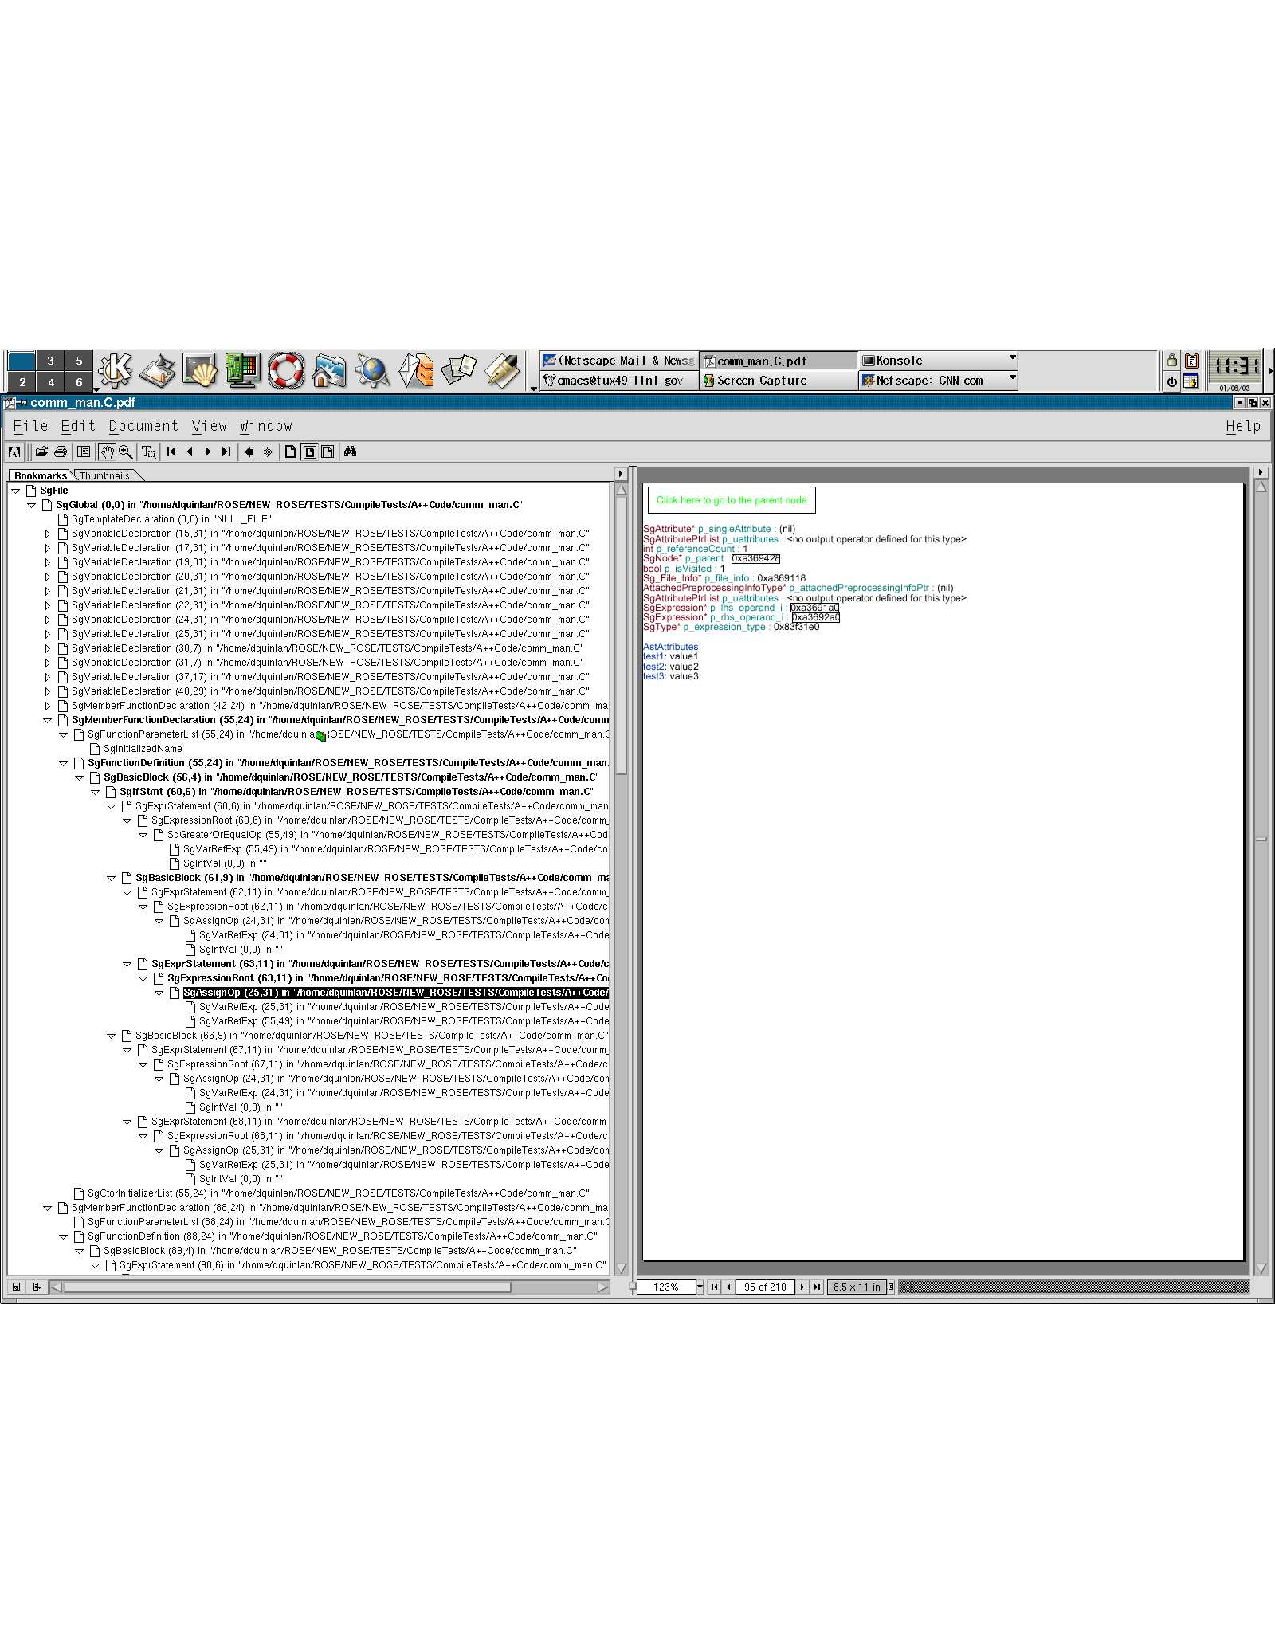
\includegraphics[angle=90,scale=0.85]{\TranslatorExampleDirectory/AST-pdf2}
\caption{Example output from translator which outputs PDF representation of AST. The
    generated PDF file makes use of the bookmark mechanism to expand and collapse 
    parts of the AST.}
\label{tutorial:exampleOutputCodePDF}
\end{figure}

The program in figure~\ref{Tutorial:exampleAST_PDF_Generator} calls 
an internal ROSE function that traverses the AST and generates 
an ASCI file in {\tt dot} format.
Figure~\ref{Tutorial:exampleInputCode_ASTGraphGenerator} shows an input
code which is processed to generate a graph of the AST, generating a 
{\tt pdf} file.   The {\tt pdf} file is then processed
using {\tt acroread} to generate a GUI for viewing the AST.

A standalone utility tool, called \textit{pdfGenerator} is provided within
ROSE. It is available from
\textit{ROSE\_BUILD/exampleTranslators/PDFGenerator} or
\textit{ROSE\_INS/bin}. Users can use it to generate AST in a pdf format
from an input code.

   Figure~\ref{tutorial:exampleOutputCodePDF} displays on the left hand side the individual
C++ nodes in ROSE's intermediate representation (IR).  The page on the right hand side
shows that IR nodes member data. Pointers in boxes can be clicked on to navigate the AST
(or nodes in the tree hierarchy can be clicked on jump to any location in the AST.
This representation shows only the IR nodes that are traversed by the standard traversal
(no SgSymbol or SgType IR nodes are presented in this view of the AST).

% Alternative description
The output of this translator is shown in figure \ref{tutorial:exampleOutputCodePDF}.  The left hand side
of the screen is a tree with click-able nodes to expand/collapse the subtrees.
The right hand side of the screen is a description of the data at a particular 
node in the AST (the node where the user has clicked the left mouse button).
This relatively simple view of the AST is useful for debugging transformation and finding
information in the AST required by specific sorts of analysis.  It is also useful
for developing an intuitive feel for what information is in the AST, how it is organized, 
and where it is stored.


\chapter{Introduction to AST Traversals}
\label{chap:traversals}

% Suggestions from discussions with Jim McGraw about this chapter.
\fixme{Add {\bf What to learn from this example} paragraph to each example.}
\fixme{Add {\bf What is different from previous example} paragraph to each example.}
\fixme{Add a table and/or graph at the end of this chapter to summarize the traversals.}

    An essential operation in the analysis and construction of ASTs is the
definition of traversals upon the AST to gather information and modify
targeted internal representation (IR) nodes.  ROSE includes different
sorts of traversals to address the different requirements of numerous
program analysis and transformation operations.  This section demonstrates
the different types of traversals that are possible using ROSE.

    ROSE translators most commonly introduce transformations and analysis
through a traversal over the AST.  Alternatives could be to generate
a simpler IR that is more suitable to a specific transformation and
either convert modification to that transformation specific IR
into changes to the AST or generate source code from the transformation specific
IR directly.  These approaches are more complex than introducing changes
to the AST directly, but may be better for specific transformations.

   Traversals represent an essential operation on the AST and there are a
number of different types of traversals.  The suggested traversals for users
are explained in Section~\ref{Tutorial:astStructureTraversals}.
Section~\ref{Tutorial:memoryPoolTraversals} introduces specialized traversals
(that traverse the AST in different orders and traverse types and symbols),
typically not appropriate for most translators (but perhaps appropriate for
specialized tools, often internal tools within ROSE).

See the ROSE User Manual for a more complete introduction to the different types of
traversals.  The purpose of this tutorial is to present examples, but we focus less on
the background and philosophy here than in the ROSE User Manual.

% GB (9/10/2007): I think these points are now taken care of.
%\fixme{Comments from Jacob:
%    1) Describe what the traversals are used for.
%    2) Reference ROSE User Manual.
%  }

   This chapter presents a number of ways of traversing the AST
of any input source code.  These {\em traversals} permit operations
on the AST, which may either read or modify the AST in place.  Modifications
to the AST will be reflected in the source code generated when the AST is 
{\em unparsed}; the code generation phase of the source-to-source process
defined by ROSE.  Note that for all examples, the input code described in 
section~\ref{Tutorial:exampleInputCodeDescription} is used to generate
all outputs shown with each translator.


\section{Input For Example Traversals}
\label{Tutorial:exampleInputCodeDescription}

\begin{figure}[!h]
{\indent
{\mySmallFontSize

% Do this when processing latex to generate non-html (not using latex2html)
\begin{latexonly}
   \lstinputlisting{\TutorialExampleDirectory/inputCode_ExampleTraversals.C}
\end{latexonly}

% Do this when processing latex to build html (using latex2html)
\begin{htmlonly}
   \verbatiminput{\TutorialExampleDirectory/inputCode_ExampleTraversals.C}
\end{htmlonly}

% end of scope in font size
}
% End of scope in indentation
}
\caption{Example source code used as input to program in
         traversals shown in this chapter.}
\label{Tutorial:exampleInputCode_ExampleTraversals}
\end{figure}

   The code shown in figure~\ref{Tutorial:exampleInputCode_ExampleTraversals}
shows the input code that will be used to demonstrate the traversals in this 
chapter.  It may be modified by the user to experiment with the use of the traversals
on alternative input codes.


%\clearpage
\section{Traversals of the AST Structure}
\label{Tutorial:astStructureTraversals}

    This collection of traversals operates on the AST in an order
which matches the structure of the AST and the associated source code.
These types of traversals are the most common traversals for users
to use.  A subsequent section of this chapter demonstrated more
specialized traversals over all IR nodes (more than just those IR nodes
in the AST representing the structure of the source code) that are 
suitable for some tools, mostly tools built internally within ROSE.

   Because the traversals in this section traverse the structure of
the source code (see the AST graph presented in the first tutorial 
example) they are more appropriate for most transformations
of the source code.  We suggest that the user focus on these 
traversals which represent the interface we promote for analysis
and transformation of the AST, instead of the memory pools traversals
which are suitable mostly for highly specialized internal tools.
The simple traversals of both kinds have the same interface so the user may
easily switch between them with out significant difficulty.

% \clearpage
% \subsection{Classic Object-Oriented Visitor Pattern for the AST (Not Yet Implemented)}
\subsection{Classic Object-Oriented Visitor Pattern for the AST}

   We show this example first, but it is rarely used in practice, and
more useful traversals follow.  It is however most closely similar to
traversals that are available in other compiler infrastructures, and so
a concept with which many people will be familar.  In this case because
this implementation is based on the memory pool infrstructure it will
visit all node and not in any order based on the AST.  The ASTSimpleProcessing
traversal in section~\ref{ASTSimpleProcessing_traversal} is closer to a common 
visitor pattern that visits the IR nodes in the order in which they appear in 
the AST.

\begin{figure}[!h]
{\indent
{\mySmallFontSize

% Do this when processing latex to generate non-html (not using latex2html)
\begin{latexonly}
   \lstinputlisting{\TutorialExampleDirectory/classicObjectOrientedVisitorPatternMemoryPoolTraversal.C}
\end{latexonly}

% Do this when processing latex to build html (using latex2html)
\begin{htmlonly}
   \verbatiminput{\TutorialExampleDirectory/classicObjectOrientedVisitorPatternMemoryPoolTraversal.C}
\end{htmlonly}

% end of scope in font size
}
% End of scope in indentation
}
\caption{Example source showing simple visitor pattern.}
\label{Tutorial:exampleClassicVisitorPattern}
\end{figure}

% (09/10/2019) Pei-Hung remove the following because it cannot be generated to PDF due to size limit
\commentout{
\begin{figure}[!h]
{\indent
{\mySmallFontSize


% Do this when processing latex to generate non-html (not using latex2html)
\begin{latexonly}
   \lstinputlisting{\TutorialExampleBuildDirectory/classicObjectOrientedVisitorPatternMemoryPoolTraversal.out}
\end{latexonly}

% Do this when processing latex to build html (using latex2html)
\begin{htmlonly}
   \verbatiminput{\TutorialExampleBuildDirectory/classicObjectOrientedVisitorPatternMemoryPoolTraversal.out}
\end{htmlonly}

% end of scope in font size
}
% End of scope in indentation
}
\caption{Output of input file to the visitor pattern traversal over the memory pools.}
\label{Tutorial:exampleOutput_ClassicVisitorPattern}
\end{figure}
}

Figure~\ref{Tutorial:exampleClassicVisitorPattern} shows the source code 
for a translator using the classic object-oriented visitor pattern 
to traverse the AST.  {\em This visitor pattern is only implemented
for the memory pool based traversal.}  Thus it works on the whole
of the attributed AST and does not work on a restricted subset of 
the AST (e.g. a subtree of the unattributed AST).
% It is however expected to appear identical to the classing visitor pattern 
% shown for the memory pool traversal.} 
% (09/10/2019) Pei-Hung remove the following because the output example is removed
\commentout{
Figure~\ref{Tutorial:exampleOutput_ClassicVisitorPattern} shows the 
output from this traversal using the example input source from 
figure~\ref{Tutorial:exampleInputCode_ExampleTraversals}.
}


% \clearpage
\subsection{Simple Traversal (no attributes)}
\label{ASTSimpleProcessing_traversal}

\begin{figure}[!h]
{\indent
{\mySmallFontSize

% Do this when processing latex to generate non-html (not using latex2html)
\begin{latexonly}
   \lstinputlisting{\TutorialExampleDirectory/visitorTraversal.C}
\end{latexonly}

% Do this when processing latex to build html (using latex2html)
\begin{htmlonly}
   \verbatiminput{\TutorialExampleDirectory/visitorTraversal.C}
\end{htmlonly}

% end of scope in font size
}
% End of scope in indentation
}
\caption{Example source showing simple visitor pattern.}
\label{Tutorial:exampleVisitorTraversal}
\end{figure}


\begin{figure}[!h]
{\indent
{\mySmallFontSize


% Do this when processing latex to generate non-html (not using latex2html)
\begin{latexonly}
   \lstinputlisting{\TutorialExampleBuildDirectory/visitorTraversal.out}
\end{latexonly}

% Do this when processing latex to build html (using latex2html)
\begin{htmlonly}
   \verbatiminput{\TutorialExampleBuildDirectory/visitorTraversal.out}
\end{htmlonly}

% end of scope in font size
}
% End of scope in indentation
}
\caption{Output of input file to the visitor traversal.}
\label{Tutorial:exampleOutput_VisitorTraversal}
\end{figure}

Figure~\ref{Tutorial:exampleVisitorTraversal} shows the source code 
for a translator which traverses the AST.  The traversal object is
from the type {\tt visitorTraversal} derived from {\tt AstSimpleProcessing}.
The {\tt visit()} function is required to be defined because it is 
defined as a pure virutal funciton in the {\tt AstSimpleProcessing} base class.
The member function {\tt traverseInputFiles()} of {\tt AstSimpleProcessing} 
is called to traverse the AST and call the {\tt visit()} function on each
IR node.  Note that the function {\tt traverse()} (not used) would visit
each IR nodes while {\tt traverseInputFiles()} will only visit those
IR nodes that originate in the input source code (thus skipping all 
header files).

For each node where the {\tt visit()} function is called a {\tt SgNode} 
pointer is to the node is passed into the {\tt visit} function.
% using only the input information represented by the current node.
Note that using this simple traversal
the only context information available to the visit function is what is stored
in its member variables (though access to other nodes is possible along
any edges in the attributed AST graph).
The only option is to traverse the AST in either pre-order or postorder.
The {\tt atTraversalEnd()} function may be defined by the user to do final
processing after all nodes have been visited (or to perform preparations
before the nodes are visited, in the case of the corresponding {\tt
atTraversalStart()} function).
Figure~\ref{Tutorial:exampleOutput_VisitorTraversal} shows the 
output from this traversal using the example input source from 
figure~\ref{Tutorial:exampleInputCode_ExampleTraversals}.

\subsection{Simple Pre- and Postorder Traversal}

\begin{figure}[!h]
{\indent
{\mySmallFontSize

% Do this when processing latex to generate non-html (not using latex2html)
\begin{latexonly}
   \lstinputlisting{\TutorialExampleDirectory/prePostTraversal.C}
\end{latexonly}

% Do this when processing latex to build html (using latex2html)
\begin{htmlonly}
   \verbatiminput{\TutorialExampleDirectory/prePostTraversal.C}
\end{htmlonly}

% end of scope in font size
}
% End of scope in indentation
}
\caption{Example source showing simple pre- and postorder pattern.}
\label{Tutorial:examplePrePostTraversal}
\end{figure}


\begin{figure}[!h]
{\indent
{\mySmallFontSize


% Do this when processing latex to generate non-html (not using latex2html)
\begin{latexonly}
   \lstinputlisting{\TutorialExampleBuildDirectory/prePostTraversal.out}
\end{latexonly}

% Do this when processing latex to build html (using latex2html)
\begin{htmlonly}
   \verbatiminput{\TutorialExampleBuildDirectory/prePostTraversal.out}
\end{htmlonly}

% end of scope in font size
}
% End of scope in indentation
}
\caption{Output of input file to the pre- and postorder traversal.}
\label{Tutorial:exampleOutput_PrePostTraversal}
\end{figure}

Figure~\ref{Tutorial:examplePrePostTraversal} shows the source code for a
translator that traverses the AST without attributes (like the one in the
previous subsection), but visiting each node twice, once in preorder (before
its children) and once in postorder (after all children).
Figure~\ref{Tutorial:exampleOutput_PrePostTraversal} shows the 
output from this traversal using the example input source from 
figure~\ref{Tutorial:exampleInputCode_ExampleTraversals}.


% \clearpage
\subsection{Inherited Attributes}

\begin{figure}[!h]
{\indent
{\mySmallFontSize


% Do this when processing latex to generate non-html (not using latex2html)
\begin{latexonly}
   \lstinputlisting{\TutorialExampleDirectory/inheritedAttributeTraversal.C}
\end{latexonly}

% Do this when processing latex to build html (using latex2html)
\begin{htmlonly}
   \verbatiminput{\TutorialExampleDirectory/inheritedAttributeTraversal.C}
\end{htmlonly}

% end of scope in font size
}
% End of scope in indentation
}
\caption{Example source code showing use of inherited attributes (passing context
         information {\bf down} the AST.}
\label{Tutorial:exampleInheritedAttributeTraversal}
\end{figure}

\begin{figure}[!h]
{\indent
{\mySmallFontSize


% Do this when processing latex to generate non-html (not using latex2html)
\begin{latexonly}
   \lstinputlisting{\TutorialExampleBuildDirectory/inheritedAttributeTraversal.out}
\end{latexonly}

% Do this when processing latex to build html (using latex2html)
\begin{htmlonly}
   \verbatiminput{\TutorialExampleBuildDirectory/inheritedAttributeTraversal.out}
\end{htmlonly}

% end of scope in font size
}
% End of scope in indentation
}
\caption{Output of input file to the inherited attribute traversal.}
\label{Tutorial:exampleOutput_InheritedAttributeTraversal}
\end{figure}

Figure~\ref{Tutorial:exampleInheritedAttributeTraversal} shows the use
of inherited attributes associated with each IR node.  Within this
traversal the attributes are managed by the traversal and exist on the
stack.  Thus the lifetime of the attributes is only as long as the
processing of the IR node and its subtree.  Attributes such as this
are used to communicate context information {\bf down} the AST and
called {\em Inherited attributes}.

In the example the class \verb+Inherited Attribute+ is used to represent 
inherited attribute. Each instance of the class represents an attribute 
value. When the AST is traversed we obtain as output the loop nest depth 
at each point in the AST. The output uses the example input source from 
figure~\ref{Tutorial:exampleInputCode_ExampleTraversals}.

Note that inherited attributes are passed by-value down the AST. In very rare
cases you might want to pass a pointer to dynamically allocated memory as an
inherited attribute. In this case you can define the virtual member function
{\tt void destroyInheritedValue(SgNode *n, InheritedAttribute inheritedValue)}
which is called after the last use of the inherited attribute computed at this
node, i.\,e.~after all children have been visited. You can use this function
to free the memory allocated for this inherited attribute.




\clearpage
\subsection{Synthesized Attributes}

\begin{figure}[!h]
{\indent
{\mySmallFontSize


% Do this when processing latex to generate non-html (not using latex2html)
\begin{latexonly}
   \lstinputlisting{\TutorialExampleDirectory/synthesizedAttributeTraversal.C}
\end{latexonly}

% Do this when processing latex to build html (using latex2html)
\begin{htmlonly}
   \verbatiminput{\TutorialExampleDirectory/synthesizedAttributeTraversal.C}
\end{htmlonly}

% end of scope in font size
}
% End of scope in indentation
}
\caption{Example source code showing use of synthesized attributed (passing analysis
         information {\bf up} the AST).}
\label{Tutorial:exampleSynthesizedAttributeTraversal}
\end{figure}

\begin{figure}[!h]
{\indent
{\mySmallFontSize


% Do this when processing latex to generate non-html (not using latex2html)
\begin{latexonly}
   \lstinputlisting{\TutorialExampleBuildDirectory/synthesizedAttributeTraversal.out}
\end{latexonly}

% Do this when processing latex to build html (using latex2html)
\begin{htmlonly}
   \verbatiminput{\TutorialExampleBuildDirectory/synthesizedAttributeTraversal.out}
\end{htmlonly}

% end of scope in font size
}
% End of scope in indentation
}
\caption{Output of input file to the synthesized attribute traversal.}
\label{Tutorial:exampleOutput_SynthesizedAttributeTraversal}
\end{figure}

  Figure~\ref{Tutorial:exampleSynthesizedAttributeTraversal} shows the use of
attributes to pass information {\bf up} the AST.  The lifetime of the attributes
are similar as for inherited attributes.  Attributes such as these are called
synthesized attributes.  

   This code shows the code for a translator which does an analysis of 
an input source code to determine the presence of loops.  It returns true if
a loop exists in the input code and false otherwise.  The list of synthesized
attributes representing the information passed up the AST from a node's
children is of type {\tt SynthesizedAttributesList}, which is a type that
behaves very similarly to {\tt vector<SynthesizedAttribute>} (it supports
iterators, can be indexed, and can be used with STL algorithms).

   The example determines the existence of loops for a given program.



\clearpage
\subsection{Accumulator Attributes}

\begin{figure}[!h]
{\indent
{\mySmallFontSize


% Do this when processing latex to generate non-html (not using latex2html)
\begin{latexonly}
   \lstinputlisting{\TutorialExampleDirectory/accumulatorAttributeTraversal.C}
\end{latexonly}

% Do this when processing latex to build html (using latex2html)
\begin{htmlonly}
   \verbatiminput{\TutorialExampleDirectory/accumulatorAttributeTraversal.C}
\end{htmlonly}

% end of scope in font size
}
% End of scope in indentation
}
\caption{Example source code showing use of accumulator attributes (typically to count
    things in the AST).}
\label{Tutorial:exampleAccumulatorAttributeTraversal}
\end{figure}


\begin{figure}[!h]
{\indent
{\mySmallFontSize


% Do this when processing latex to generate non-html (not using latex2html)
\begin{latexonly}
   \lstinputlisting{\TutorialExampleBuildDirectory/accumulatorAttributeTraversal.out}
\end{latexonly}

% Do this when processing latex to build html (using latex2html)
\begin{htmlonly}
   \verbatiminput{\TutorialExampleBuildDirectory/accumulatorAttributeTraversal.out}
\end{htmlonly}

% end of scope in font size
}
% End of scope in indentation
}
\caption{Output of input file to the accumulator attribute traversal.}
\label{Tutorial:exampleOutput_AccumulatorAttributeTraversal}
\end{figure}

   Figure~\ref{Tutorial:exampleAccumulatorAttributeTraversal} shows the use of
a different sort of attribute.  This attribute has a lifetime equal to the
lifetime of the traversal object (much longer than the traversal of any subset 
of IR nodes).  The same attribute is accessible from each IR node.  Such 
attributes are called {\em accumulator} attributes and are semantically 
equivalent to a global variable. Accumulator attributes
act as global variables which can easily be used to count application 
specific properties within the AST. 

Note that due to the limitation that the computation of inherited attributes cannot be made dependent on the values of synthesized attributes, counting operations cannot be implemented by combining these attributes as is usually done in attribute grammars. However, the use of accumulator attributes serves well for this purpose. Therefore all counting-like operations should be implemented using accumulator attributes (= member variables of traversal or processing classes).

     Although not shown in this tutorial explicitly, accumulator attributes
may be easily mixed with inherited and/or synthesized attributes.

In this example we count the number of for-loops in an input program.







% DQ (9/3/2006): We need an example of this for completeness.
% We can replace the current version with a newer version from 
% Markus when it is available.
% MS: commented out the following section because the implementation
% is not finished yet. Also, this case is covered by the new example
% loopNestingInfoProcessing which I've just added.
% GB (9/10/2007): Provided a simple example for this section.
% \commentout{
% \clearpage
\subsection{Inherited and Synthesized Attributes}

\begin{figure}[!h]
{\indent
{\mySmallestFontSize


% Do this when processing latex to generate non-html (not using latex2html)
\begin{latexonly}
   \lstinputlisting{\TutorialExampleDirectory/inheritedAndSynthesizedAttributeTraversal.C}
%  \lstinputlisting{\TutorialExampleBuildDirectory/inheritedAndSynthesizedAttributeTraversal.aa}
\end{latexonly}

% Do this when processing latex to build html (using latex2html)
\begin{htmlonly}
   \verbatiminput{\TutorialExampleDirectory/inheritedAndSynthesizedAttributeTraversal.C}
\end{htmlonly}

% end of scope in font size
}
% End of scope in indentation
}
\caption{Example source code showing use of both inherited and synthesized attributes
         working together (part 1).}
\label{Tutorial:exampleInheritedAndSynthesizedAttributeTraversal-part1}
\end{figure}

\commentout{
\begin{figure}[!h]
{\indent
{\mySmallestFontSize

% Do this when processing latex to generate non-html (not using latex2html)
\begin{latexonly}
   \lstinputlisting{\TutorialExampleBuildDirectory/inheritedAndSynthesizedAttributeTraversal.ab}
\end{latexonly}

% Do this when processing latex to build html (using latex2html)
\begin{htmlonly}
   \verbatiminput{\TutorialExampleDirectory/inheritedAndSynthesizedAttributeTraversal.C}
\end{htmlonly}

% end of scope in font size
}
% End of scope in indentation
}
\caption{Example source code showing the use of both inherited and synthesized attributes
         working together (part 2).}
\label{Tutorial:exampleInheritedAndSynthesizedAttributeTraversal-part2}
\end{figure}

% commented out
}

\begin{figure}[!h]
{\indent
{\mySmallFontSize

% Do this when processing latex to generate non-html (not using latex2html)
\begin{latexonly}
   \lstinputlisting{\TutorialExampleBuildDirectory/inheritedAndSynthesizedAttributeTraversal.out}
\end{latexonly}

% Do this when processing latex to build html (using latex2html)
\begin{htmlonly}
   \verbatiminput{\TutorialExampleBuildDirectory/inheritedAndSynthesizedAttributeTraversal.out}
\end{htmlonly}

% end of scope in font size
}
% End of scope in indentation
}
\caption{Output of input file to the inherited and synthesized attribute traversal.}
\label{Tutorial:exampleOutput_InheritedAndSynthesizedAttributeTraversal}
\end{figure}

   Figure~\ref{Tutorial:exampleInheritedAndSynthesizedAttributeTraversal-part1}
shows the combined use of inherited and synthesized attributes.  The example
source code shows the mixed use of such attributes to list the functions 
containing loop.  Inherited attributes are used to communicate that 
the traversal is in a function, which the synthesized attributes are
used to pass back the existence of loops deeper within the subtrees
associated with each function.

    List of functions containing loops.

% DQ (9/3/2006): uncommented by Dan.
% Commented out by Markus because it is not finished
% }






\clearpage
\subsection{Persistent Attributes}

\begin{figure}[!h]
{\indent
{\mySmallFontSize


% Do this when processing latex to generate non-html (not using latex2html)
\begin{latexonly}
   \lstinputlisting{\TutorialExampleDirectory/persistantAttributes.C}
\end{latexonly}

% Do this when processing latex to build html (using latex2html)
\begin{htmlonly}
   \verbatiminput{\TutorialExampleDirectory/persistantAttributes.C}
\end{htmlonly}

% end of scope in font size
}
% End of scope in indentation
}
\caption{Example source code showing use of persistent attributes used to pass information
         across multiple passes over the AST.}
\label{Tutorial:examplePersistentAttributes}
\end{figure}


\begin{figure}[!h]
{\indent
{\mySmallFontSize

% Do this when processing latex to generate non-html (not using latex2html)
\begin{latexonly}
   \lstinputlisting{\TutorialExampleBuildDirectory/persistantAttributes.out}
\end{latexonly}

% Do this when processing latex to build html (using latex2html)
\begin{htmlonly}
   \verbatiminput{\TutorialExampleBuildDirectory/persistantAttributes.out}
\end{htmlonly}

% end of scope in font size
}
% End of scope in indentation
}
\caption{Output of input file to the persistent attribute traversal showing the passing of
    information from one AST traversal to a second AST traversal.}
\label{Tutorial:exampleOutput_PersistentAttributes}
\end{figure}

     Figure~\ref{Tutorial:examplePersistentAttributes} shows the use of
another form of attribute.  This attribute has a lifetime which is controlled explicitly
by the user; it lives on the heap typically.  These attributes are explicitly attached to 
the IR nodes and are not managed directly by the traversal.  There attributes are
called {\em persistent} attributes and are not required to be associated with any
traversal.  Persistent attributes are useful for storing information across multiple
traversals (or permanently within the AST) for later traversal passes.  

   Persistent attributes may be used at any time and combined with other traversals
(similar to accumulator attributes).  Traversals may combine any or all of the
types of attributes within in ROSE as needed to store, gather, or propagate
information within the AST for complex program analysis.







\clearpage
\subsection{Nested Traversals}

\begin{figure}[!h]
{\indent
{\mySmallFontSize


% Do this when processing latex to generate non-html (not using latex2html)
\begin{latexonly}
   \lstinputlisting{\TutorialExampleDirectory/nestedTraversal.C}
\end{latexonly}

% Do this when processing latex to build html (using latex2html)
\begin{htmlonly}
   \verbatiminput{\TutorialExampleDirectory/nestedTraversal.C}
\end{htmlonly}

% end of scope in font size
}
% End of scope in indentation
}
\caption{Example source code showing use nested traversals.}
\label{Tutorial:exampleNestedTraversal}
\end{figure}


\begin{figure}[!h]
{\indent
{\mySmallFontSize

% Do this when processing latex to generate non-html (not using latex2html)
\begin{latexonly}
   \lstinputlisting{\TutorialExampleBuildDirectory/nestedTraversal.out}
\end{latexonly}

% Do this when processing latex to build html (using latex2html)
\begin{htmlonly}
   \verbatiminput{\TutorialExampleBuildDirectory/nestedTraversal.out}
\end{htmlonly}

% end of scope in font size
}
% End of scope in indentation
}
\caption{Output of input file to the nested traversal example.}
\label{Tutorial:exampleOutput_NestedTraversal}
\end{figure}

     Figure~\ref{Tutorial:exampleNestedTraversal} shows the use of multiple 
traversals in composition. Figure~\ref{Tutorial:exampleOutput_NestedTraversal}
shows the output of the nested traversal.





\clearpage
\subsection{Combining all Attributes and Using Primitive Types}

\begin{figure}[!h]
{\indent
{\mySmallFontSize


% Do this when processing latex to generate non-html (not using latex2html)
\begin{latexonly}
   \lstinputlisting{\TutorialExampleDirectory/inputCode_loopNestingInfoProcessing.C}
\end{latexonly}

% Do this when processing latex to build html (using latex2html)
\begin{htmlonly}
   \verbatiminput{\TutorialExampleDirectory/inputCode_loopNestingInfoProcessing.C}
\end{htmlonly}
}
}
\caption{Input code with nested loops for nesting info processing}
\label{Tutorial:exampleInputCode_ExampleLoopNestingInfoProcessing}
\end{figure}

\begin{figure}[!h]
{\indent
{\mySmallFontSize

% Do this when processing latex to generate non-html (not using latex2html)
\begin{latexonly}
   \lstinputlisting{\TutorialExampleBuildDirectory/loopNestingInfoProcessing.aa}
\end{latexonly}

% Do this when processing latex to build html (using latex2html)
\begin{htmlonly}
   \verbatiminput{\TutorialExampleDirectory/loopNestingInfoProcessing.C}
\end{htmlonly}

% end of scope in font size
}
% End of scope in indentation
}
\caption{Example source code showing use of inherited, synthesized, accumulator, and persistent attributes (part 1).}
\label{Tutorial:exampleLoopNestingInfoProcessing}
\end{figure}



\begin{latexonly}
\begin{figure}[!h]
{\indent
{\mySmallFontSize

   \lstinputlisting{\TutorialExampleBuildDirectory/loopNestingInfoProcessing.ab}
% end of scope in font size
}
% End of scope in indentation

}\caption{Example source code showing use of inherited, synthesized, accumulator, and persistent attributes (part 2).}
\label{Tutorial:exampleLoopNestingInfoProcessing2}
\end{figure}
\end{latexonly}


\begin{figure}[!h]
{\indent
{\mySmallFontSize

% Do this when processing latex to generate non-html (not using latex2html)
\begin{latexonly}
   \lstinputlisting{\TutorialExampleBuildDirectory/loopNestingInfoProcessing.out}
\end{latexonly}

% Do this when processing latex to build html (using latex2html)
\begin{htmlonly}
   \verbatiminput{\TutorialExampleBuildDirectory/loopNestingInfoProcessing.out}
\end{htmlonly}

% end of scope in font size
}
% End of scope in indentation
}
\caption{Output code showing the result of using inherited, synthesized, and accumulator attributes.}
\label{Tutorial:exampleOutput_loopNestingInfoProcessing}
\end{figure}

The previous examples have shown cases where attributes were classes,
alternatively attributes can be any primitive type (int, bool,
etc.). This example demonstrates how to use
AstTopDownBottomUpProcessing to compute inherited and synthesized
attributes, generate pdf and dot output, how to accumulate
information, and how to attach attributes to AST nodes in the same
pass.

The attributes are used to compute the nesting level and the nesting
depth of for/while/do-while loops: The nesting level is computed using
an inherited attribute. It holds that $nesting-level(innerloop) =
nesting-level(outerloop) + 1$ starting with 1 at the outer most loop.
The nesting depth is computed using a synthesized attribute. It holds
that $nesting-depth(innerloop) = nesting-level(outerloop) - 1$
starting with 1 at the inner most loop.

To compute the values we use a primitive type (unsigned int). This
example also shows how to use defaultSynthesizedAttribute to
initialize a synthesized attribute of primitive type. The values of
the attributes are attached to the AST using AstAttribute and the AST
node attribute mechanism available at every AST node (which can be
accessed with \verb+node->attribute+).  (see
loopNestingInfoProcessing.C)

For the entire program the maximum nesting level (= max nesting depth)
is computed as accumulated value using member variable
\verb+_maxNestingLevel+ of class LoopNestingInfoProcessing. We also
demonstrate how to customize an AstAttribute such that the value of
the attribute is printed in a pdf output.  (by overriding toString,
see LoopNestingInfo class)

In the generated pdf file (for some C++ input file) the values of the
attributes can be viewed for each node (see printLoopInfo
implementation). Further more we also generate a dot file, to
visualize the tree using the graph visualization tool dot. The
generated file can be converted to postscript (using dot) and viewed
with gv.

\subsection{Combined Traversals}

Performing a large number of program analyses as separate traversals of the
AST can be somewhat inefficient as there is some overhead associated with
visiting every node several times. ROSE therefore provides a mechanism for
combining traversal objects of the same base type and evaluating them in a
single traversal of the AST. This is entirely transparent to the individual
traversal object, so existing code can be reused with the combination
mechanism, and analyzers can be developed and tested in isolation and combined
when needed.

The one requirement that is placed on traversals to be combined is that they
be independent of each other; in particular, this means that they should not
modify the AST or any shared global data. Any output produced by the analyzers
will be interleaved.

\begin{figure}[!h]
{\indent
{\mySmallFontSize

% Do this when processing latex to generate non-html (not using latex2html)
\begin{latexonly}
   \lstinputlisting{\TutorialExampleDirectory/combinedTraversals.C}
\end{latexonly}

% Do this when processing latex to build html (using latex2html)
\begin{htmlonly}
   \verbatiminput{\TutorialExampleDirectory/combinedTraversals.C}
\end{htmlonly}

% end of scope in font size
}
% End of scope in indentation
}
\caption{Example source showing the combination of traversals.}
\label{Tutorial:exampleCombinedTraversals}
\end{figure}


\begin{figure}[!h]
{\indent
{\mySmallFontSize


% Do this when processing latex to generate non-html (not using latex2html)
\begin{latexonly}
   \lstinputlisting{\TutorialExampleBuildDirectory/combinedTraversals.out}
\end{latexonly}

% Do this when processing latex to build html (using latex2html)
\begin{htmlonly}
   \verbatiminput{\TutorialExampleBuildDirectory/combinedTraversals.out}
\end{htmlonly}

% end of scope in font size
}
% End of scope in indentation
}
\caption{Output of input file to the combined traversals. Note that the order
of outputs changes as execution of several analyzers is interleaved.}
\label{Tutorial:exampleOutput_CombinedTraversals}
\end{figure}

Figure~\ref{Tutorial:exampleCombinedTraversals} shows the source code for a
translator that combines three different analyzers into one traversal, each
one counting the occurrences of a different type of AST node (as determined by
a VariantT value). First three traversals are run after each other, as usual;
then three traversal objects are passed (by pointer) to an object of type {\tt
AstCombinedSimpleProcessing} using its {\tt addTraversal} method. One then
invokes one of the usual traverse methods on this combined object with the
same effect as if it had been called for each of the traversal objects
individually.

Any operation on the list of analyzers is possible using the {\tt
get\_traversalPtrListRef} method of the combined processing class that returns
a reference to its internal list of analyzers (an object of type {\tt
vector<AstSimpleProcessing *>}). Any changes made through this reference will
be reflected in further traversals.

In addition to {\tt AstCombinedSimpleProcessing}, there is also a combined
class for each of the other types of traversals discussed above: {\tt
AstCombinedTopDownProcessing}, {\tt AstCombinedBottomUpProcessing}, etc. Where
traversals using attributes are combined, all of the combined traversals must
have the same attribute types (i.\,e.~the same template parameters). Attributes
are passed to and returned from the combined traversal as a vector.

\clearpage
\subsection{Short-Circuiting Traversals}

   The traversal short-circuit mechanism is a simple way to cut short
the traversal of a large AST once specific information has been obtained.
It is purely an optimization mechanism, and a bit of a hack, but common
within the C++ Boost community.  Since the technique works we present it
as a way of permitting users to avoid the full traversal of an AST
that they might deam to be redundant of inappropriate.  We don't
expect that this mechanism will be particularly useful to most users
and we don't recommend it.  It may even at some point not be supported.
However, we present it because it is a common technique used in the C++ 
Boost community and it happens to work (at one point it didn't work and
so we have no idea what we fixed that permitted it to work now).  We have
regarded this technique as a rather ugly hack.  It is presented in case
you really need it.  It is, we think, better than the direct use of lower
level mechanisms that are used to support the AST traversal.

\begin{figure}[!h]
{\indent
{\mySmallFontSize

% Do this when processing latex to generate non-html (not using latex2html)
\begin{latexonly}
   \lstinputlisting{\TutorialExampleDirectory/inputCode_traversalShortCircuit.C}
\end{latexonly}

% Do this when processing latex to build html (using latex2html)
\begin{htmlonly}
   \verbatiminput{\TutorialExampleDirectory/inputCode_traversalShortCircuit.C}
\end{htmlonly}
}
}
\caption{Input code with used to demonstrate the traversal short-circuit mechanism.}
\label{Tutorial:exampleInputCode_ExampleLoopNestingInfoProcessing}
\end{figure}

\begin{figure}[!h]
{\indent
{\mySmallFontSize

% Do this when processing latex to generate non-html (not using latex2html)
\begin{latexonly}
   \lstinputlisting{\TutorialExampleDirectory/traversalShortCircuit.C}
\end{latexonly}

% Do this when processing latex to build html (using latex2html)
\begin{htmlonly}
   \verbatiminput{\TutorialExampleDirectory/traversalShortCircuit.C}
\end{htmlonly}

% end of scope in font size
}
% End of scope in indentation
}
\caption{Example source code showing use of short-circuit mechanism to avoid traversal of full AST.}
\label{Tutorial:exampleTraversalShortCircuit}
\end{figure}

Figure~\ref{Tutorial:exampleTraversalShortCircuit} shows the example code demonstrating a
traversal setup to support the short-circuit mechanism (a conventional mechanism used
often within the C++ Boost community). The input code shown in 
figure~\ref{Tutorial:exampleInputCode_ExampleLoopNestingInfoProcessing}
is compiled using the example translator, the output is shown in 
figure~\ref{Tutorial:exampleOutput_traversalShortCircuit}.

\begin{figure}[!h]
{\indent
{\mySmallFontSize

% Do this when processing latex to generate non-html (not using latex2html)
\begin{latexonly}
   \lstinputlisting{\TutorialExampleBuildDirectory/traversalShortCircuit.out}
\end{latexonly}

% Do this when processing latex to build html (using latex2html)
\begin{htmlonly}
   \verbatiminput{\TutorialExampleBuildDirectory/traversalShortCircuit.out}
\end{htmlonly}

% end of scope in font size
}
% End of scope in indentation
}
\caption{Output code showing the result of short-circuiting the traversal.}
\label{Tutorial:exampleOutput_traversalShortCircuit}
\end{figure}

   The output shown in figure~\ref{Tutorial:exampleOutput_traversalShortCircuit}
demonstrates the initiation of a traversal over the AST and that traversal
being short-circuited after a specific point in the evaluation.  The result is
that there is no further traversal of the AST after that point where it is
short-circuited.




   
\clearpage
\section{Memory Pool Traversals}
\label{Tutorial:memoryPoolTraversals}

   Allocation of IR nodes in ROSE is made more efficient through the
use of specialized allocators implemented at member function new operators
for each class of the IR in Sage III.  Such specialized memory allocators 
avoid significant fragmentation of memory, provide more efficient packing 
of memory, improve performance of allocation of memory and IR node access, and additionally
provide a secondary mechanism to accessing all the IR nodes.  Each IR
node has a memory pool which is an STL vector of blocks (a fixed or variable 
sized array of contiguously stored IR nodes).  

   The three types of traversals are:
\begin{enumerate}
   \item ROSE Memory Pool Visit Traversal \\
         This traversal is similar to the one provided by the SimpleProcessing Class 
    (using the visit() function and no inherited or synthesized attributes).
   \item Classic Object-Oriented Visitor Pattern for Memory Pool \\
         This is a classic object-oriented visitor pattern.
   \item IR node type traversal, visits one type of IR node for all IR types in the AST.
         This is useful for building specialized tools.
\end{enumerate}


\subsection{ROSE Memory Pool Visit Traversal}

Figure~\ref{Tutorial:exampleMemoryPoolVisitorTraversal} shows the source code 
for a translator which traverses the memory pool containing the AST.  At each 
node the {\tt visit()} function is called using only the input information
represented by the current node.  Note that using this simple traversal
no context information is available to the visit function. 
All the IR nodes for a given memory pool are iterated over at one time.
The order of the traversal of the different memory pools is random but fixed.
Thus the order of the traversal of the IR nodes is in no way connected to the
structure of the AST (unlike the previous non-memory pool traversals that were
very much tied to the structure of the AST and which matched the structure of the 
original input source code being compiled).

\begin{figure}[!h]
{\indent
{\mySmallFontSize

% Do this when processing latex to generate non-html (not using latex2html)
\begin{latexonly}
   \lstinputlisting{\TutorialExampleDirectory/visitorMemoryPoolTraversal.C}
\end{latexonly}

% Do this when processing latex to build html (using latex2html)
\begin{htmlonly}
   \verbatiminput{\TutorialExampleDirectory/visitorMemoryPoolTraversal.C}
\end{htmlonly}

% end of scope in font size
}
% End of scope in indentation
}
\caption{Example source showing simple visit traversal over the memory pools.}
\label{Tutorial:exampleMemoryPoolVisitorTraversal}
\end{figure}



\begin{figure}[!h]
{\indent
{\mySmallFontSize


% Do this when processing latex to generate non-html (not using latex2html)
\begin{latexonly}
   \lstinputlisting{\TutorialExampleBuildDirectory/visitorMemoryPoolTraversal.out}
\end{latexonly}

% Do this when processing latex to build html (using latex2html)
\begin{htmlonly}
   \verbatiminput{\TutorialExampleBuildDirectory/visitorMemoryPoolTraversal.out}
\end{htmlonly}

% end of scope in font size
}
% End of scope in indentation
}
\caption{Output of input file to the visitor traversal over the memory pool.}
\label{Tutorial:exampleOutput_MemoryPoolVisitorTraversal}
\end{figure}


\clearpage
\subsection{Classic Object-Oriented Visitor Pattern for Memory Pool}

Figure~\ref{Tutorial:exampleMemoryPoolVisitorPattern} shows the source code 
for a translator which traverses the memory pools containing the AST.  
At each node the {\tt visit()} function is called using only the input 
information represented by the current node.  Note that using this simple 
traversal no context information is available to the visit function. 
The traversal order is the same as in the \ref{Tutorial:exampleMemoryPoolVisitorTraversal}.

\begin{figure}[!h]
{\indent
{\mySmallFontSize


% Do this when processing latex to generate non-html (not using latex2html)
\begin{latexonly}
   \lstinputlisting{\TutorialExampleDirectory/classicObjectOrientedVisitorPatternMemoryPoolTraversal.C}
\end{latexonly}

% Do this when processing latex to build html (using latex2html)
\begin{htmlonly}
   \verbatiminput{\TutorialExampleDirectory/classicObjectOrientedVisitorPatternMemoryPoolTraversal.C}
\end{htmlonly}

% end of scope in font size
}
% End of scope in indentation
}
\caption{Example source showing simple visitor pattern.}
\label{Tutorial:exampleMemoryPoolVisitorPattern}
\end{figure}


% (09/10/2019) Pei-Hung remove the following because the output example is removed
\commentout{
\begin{figure}[!h]
{\indent
{\mySmallFontSize

% Do this when processing latex to generate non-html (not using latex2html)
\begin{latexonly}
   \lstinputlisting{\TutorialExampleBuildDirectory/classicObjectOrientedVisitorPatternMemoryPoolTraversal.out}
\end{latexonly}

% Do this when processing latex to build html (using latex2html)
\begin{htmlonly}
   \verbatiminput{\TutorialExampleBuildDirectory/classicObjectOrientedVisitorPatternMemoryPoolTraversal.out}
\end{htmlonly}

% end of scope in font size
}
% End of scope in indentation
}
\caption{Output of input file to the visitor pattern traversal over the memory pools.}
\label{Tutorial:exampleOutput_MemoryPoolVisitorPattern}
\end{figure}
}

\clearpage
\subsection{ROSE IR Type Traversal (uses Memory Pools)}

Figure~\ref{Tutorial:exampleIRTypeMemoryPoolVisitorTraversal} shows the source code 
for a translator which traverses only one type of IR node using the memory pool 
containing the AST.  This traversal is useful for building specialized tools
(often tools which only call static functions on each type of IR node).

This example shows the use of an alternative traversal which traverses a 
representative of each type or IR node just one, but only if it exists
in the AST (memory pools).  This sort of traversal is useful for building
tools that need only operate on static member functions of the IR nodes
or need only sample one of each type or IR node present in the AST.
this specific example also appears in:
     {\em ROSE/src/midend/astDiagnostics/AstStatistics.C}.

The user's use of the traversal is the same as for other ROSE AST traversals
except that the ROSE\_VisitTraversal::traverseRepresentativeIRnodes() member
function is called instead of ROSE\_VisitTraversal::traverseMemoryPool().

\begin{figure}[!h]
{\indent
{\mySmallFontSize

% Do this when processing latex to generate non-html (not using latex2html)
\begin{latexonly}
   \lstinputlisting{\TutorialExampleDirectory/traverseIRnodeTypes.C}
\end{latexonly}

% Do this when processing latex to build html (using latex2html)
\begin{htmlonly}
   \verbatiminput{\TutorialExampleDirectory/traverseIRnodeTypes.C}
\end{htmlonly}

% end of scope in font size
}
% End of scope in indentation
}
\caption{Example source showing simple visit traversal over each type of IR node (one only) in the memory pools.}
\label{Tutorial:exampleIRTypeMemoryPoolVisitorTraversal}
\end{figure}


\begin{figure}[!h]
{\indent
{\mySmallFontSize

% Do this when processing latex to generate non-html (not using latex2html)
\begin{latexonly}
   \lstinputlisting{\TutorialExampleBuildDirectory/traverseIRnodeTypes.out}
\end{latexonly}

% Do this when processing latex to build html (using latex2html)
\begin{htmlonly}
   \verbatiminput{\TutorialExampleBuildDirectory/traverseIRnodeTypes.out}
\end{htmlonly}

% end of scope in font size
}
% End of scope in indentation
}
\caption{Output of input file to the IR Type traversal over the memory pool.}
\label{Tutorial:exampleOutput_IRTypeMemoryPoolVisitorTraversal}
\end{figure}

   This mechanism can be used to generate more complete reports of the memory consumption
of the AST, which is reported on if {\em -rose:verbose 2} is used.
Figure~\ref{Tutorial:exampleOutput_IRTypeMemoryUse}
shows a partial snapshot of current IR node frequency and memory consumption for
a moderate 40,000 line source code file (one file calling a number of header files),
sorted by memory consumption.  The AST contains approximately 280K IR nodes.
Note that the Sg\_File\_Info IR nodes is most frequent and consumes the greatest amount 
of memory, this reflects our bias toward preserving significant information about the
mapping of language constructs back to the positions in the source file to support
a rich set of source-to-source functionality.
{\em Note: more complete information about the memory use of the AST in in the ROSE User Manual appendix.}

\begin{figure}[!h]
{\mySmallFontSize
\begin{verbatim}
AST Memory Pool Statistics: numberOfNodes = 114081 memory consumption = 5019564 node = Sg_File_Info
AST Memory Pool Statistics: numberOfNodes =  31403 memory consumption =  628060 node = SgTypedefSeq
AST Memory Pool Statistics: numberOfNodes =  14254 memory consumption =  285080 node = SgStorageModifier
AST Memory Pool Statistics: numberOfNodes =  14254 memory consumption = 1140320 node = SgInitializedName
AST Memory Pool Statistics: numberOfNodes =   8458 memory consumption =  169160 node = SgFunctionParameterTypeList
AST Memory Pool Statistics: numberOfNodes =   7868 memory consumption = 1101520 node = SgModifierType
AST Memory Pool Statistics: numberOfNodes =   7657 memory consumption =  398164 node = SgClassType
AST Memory Pool Statistics: numberOfNodes =   7507 memory consumption = 2071932 node = SgClassDeclaration
AST Memory Pool Statistics: numberOfNodes =   7060 memory consumption =  282400 node = SgTemplateArgument
AST Memory Pool Statistics: numberOfNodes =   6024 memory consumption =  385536 node = SgPartialFunctionType
AST Memory Pool Statistics: numberOfNodes =   5985 memory consumption = 1388520 node = SgFunctionParameterList
AST Memory Pool Statistics: numberOfNodes =   4505 memory consumption = 1477640 node = SgTemplateInstantiationDecl
AST Memory Pool Statistics: numberOfNodes =   3697 memory consumption =  162668 node = SgReferenceType
AST Memory Pool Statistics: numberOfNodes =   3270 memory consumption =  758640 node = SgCtorInitializerList
AST Memory Pool Statistics: numberOfNodes =   3178 memory consumption =   76272 node = SgMemberFunctionSymbol
AST Memory Pool Statistics: numberOfNodes =   2713 memory consumption =  119372 node = SgPointerType
AST Memory Pool Statistics: numberOfNodes =   2688 memory consumption =  161280 node = SgThrowOp
AST Memory Pool Statistics: numberOfNodes =   2503 memory consumption =   60072 node = SgFunctionSymbol
AST Memory Pool Statistics: numberOfNodes =   2434 memory consumption =  107096 node = SgFunctionTypeSymbol
AST Memory Pool Statistics: numberOfNodes =   2418 memory consumption =  831792 node = SgFunctionDeclaration
AST Memory Pool Statistics: numberOfNodes =   2304 memory consumption =   55296 node = SgVariableSymbol
AST Memory Pool Statistics: numberOfNodes =   2298 memory consumption =  101112 node = SgVarRefExp
AST Memory Pool Statistics: numberOfNodes =   2195 memory consumption =  114140 node = SgSymbolTable
AST Memory Pool Statistics: numberOfNodes =   2072 memory consumption =  721056 node = SgMemberFunctionDeclaration
AST Memory Pool Statistics: numberOfNodes =   1668 memory consumption =  400320 node = SgVariableDeclaration
AST Memory Pool Statistics: numberOfNodes =   1667 memory consumption =  393412 node = SgVariableDefinition
AST Memory Pool Statistics: numberOfNodes =   1579 memory consumption =  101056 node = SgMemberFunctionType
AST Memory Pool Statistics: numberOfNodes =   1301 memory consumption =   31224 node = SgTemplateSymbol
AST Memory Pool Statistics: numberOfNodes =   1300 memory consumption =  364000 node = SgTemplateDeclaration
AST Memory Pool Statistics: numberOfNodes =   1198 memory consumption =  455240 node = SgTemplateInstantiationMemberFunctionDecl
AST Memory Pool Statistics: numberOfNodes =   1129 memory consumption =   54192 node = SgIntVal
AST Memory Pool Statistics: numberOfNodes =   1092 memory consumption =   56784 node = SgAssignInitializer
AST Memory Pool Statistics: numberOfNodes =   1006 memory consumption =   52312 node = SgExpressionRoot

Truncated results presented ...
\end{verbatim}
}
\caption{Example of output using -rose:verbose 2 (memory use report for AST).}
\label{Tutorial:exampleOutput_IRTypeMemoryUse}
\end{figure}

\chapter{Graph Processing Tutorial}

\section{Traversal Tutorial}
ROSE can collect and analyze paths in both source and binary CFGs. At moment it doesn't attempt to save paths because if
you save them directly the space necessary is extremely large, as paths grow $2^n$ with successive if statements and even faster
when for loops are involved. Currently a path can only cannot complete the same loop twice. However it is possible for a graph
such that 1 -> 2 , 2->3, 3->1, 3->5, has paths, 1,2,3,1,2,3,5 and 1,2,3,5 because the loop 1,2,3,1 is not repeated.

The tutorial example works as such:
\begin{figure}[!h]
{\indent
{\mySmallFontSize

% Do this when processing latex to generate non-html (not using latex2html)
\begin{latexonly}
   \lstinputlisting[language=C++]{\TOPSRCDIR/tutorial/sourceTraversalTutorial.C}
\end{latexonly}

% Do this when processing latex to build html (using latex2html)
\begin{htmlonly}
   \verbatiminput{\TOPSRCDIR/tutorial/sourceTraversalTutorial.C}
\end{htmlonly}

% end of scope in font size
}
% End of scope in indentation
}
\caption{Source CFG Traversal Example}
\label{Tutorial:sourceTraversalTutorial}
\end{figure}

\begin{figure}[!h]
{\indent
{\mySmallFontSize

% Do this when processing latex to generate non-html (not using latex2html)
\begin{latexonly}
   \lstinputlisting[language=C++]{\TOPSRCDIR/tutorial/binaryTraversalTutorial.C}
\end{latexonly}

% Do this when processing latex to build html (using latex2html)
\begin{htmlonly}
   \verbatiminput{\TOPSRCDIR/tutorial/binaryTraversalTutorial.C}
\end{htmlonly}

% end of scope in font size
}
% End of scope in indentation
}
\caption{Binary CFG Traversal Example}
\label{Tutorial:binaryTraversalTutorial}
\end{figure}

% the chapter talking about scope uses AST traversal
% So I moved it after the traversal chapter.  Liao 3/3/2010
\chapter{Scopes of Declarations}

     The scope of an IR node may be either stored explicitly in the IR node
or obtained through computation through its parent information in the AST.
Figure X shows an example where the variable definition for a variable is 
the scope of namespace X.  The declaration for variable a is in the namespace X.
In a more common way, the function foo is a member function of B with a
declaration appearing in class B, but with a function definition in global scope.
{\mySmallFontSize
\begin{verbatim}
namespace X{
   extern int a;
}
int X::a = 0;
class B
  {
    void foo();
  };
void B::foo() {}
\end{verbatim}
}
In C++, using name qualification the scope of a declaration can be independent of
it structural location in the AST.  The {\tt get\_parent()} member function (available 
on most IR nodes) communicates the structural information of the original source code
(also represented in the AST).  The scope information must at times be stored
explicitly when it can not be interpreted structurally.

   The example in this chapter show how to find the scope of each C++ construct
   .  Note that SgExpression IR nodes can take their scope from
that of the statement where they are found.  SgStatement and SgInitializedName
IR nodes are the interesting IR nodes from the point of scope.

   The SgInitializedName and all SgStatement IR nodes have a member function
{\tt get\_scope()} which returns the scope of the associated IR nodes.  The
example code in this chapter traverses the AST and reports the scope of any
SgInitializedName and all SgStatement IR nodes.  It is intended to provide
a simple intuition about what the scope can be expected to be in an application.
The example code is also useful as a simple means of exploring the scopes
of any other input application.

\section{Input For Examples Showing Scope Information}

   Figure~\ref{Tutorial:exampleInputCode_ScopeInformation}
shows the input example code form this tutorial example.

\begin{figure}[!h]
{\indent
{\mySmallFontSize

% Do this when processing latex to generate non-html (not using latex2html)
\begin{latexonly}
   \lstinputlisting{\TutorialExampleDirectory/inputCode_scopeInformation.C}
\end{latexonly}

% Do this when processing latex to build html (using latex2html)
\begin{htmlonly}
   \verbatiminput{\TutorialExampleDirectory/inputCode_scopeInformation.C}
\end{htmlonly}

% end of scope in font size
}
% End of scope in indentation
}
\caption{Example source code used as input to program in
         codes used in this chapter.}
\label{Tutorial:exampleInputCode_ScopeInformation}
\end{figure}


\section{Generating the code representing any IR node}

    The following code traverses each IR node and for a 
SgInitializedName of SgStatement outputs the scope information.
The input code is shown in figure \ref{Tutorial:exampleInputCode_ScopeInformation};
the output of this code is shown in figure 
\ref{Tutorial:exampleOutput_ScopeInformation}.
    
\begin{figure}[!h]
{\indent
{\mySmallFontSize


% Do this when processing latex to generate non-html (not using latex2html)
\begin{latexonly}
   \lstinputlisting{\TutorialExampleDirectory/scopeInformation.C}
\end{latexonly}

% Do this when processing latex to build html (using latex2html)
\begin{htmlonly}
   \verbatiminput{\TutorialExampleDirectory/scopeInformation.C}
\end{htmlonly}

% end of scope in font size
}
% End of scope in indentation
}
\caption{Example source code showing how to get scope information for each IR node. }
\label{Tutorial:example_ScopeInformation}
\end{figure}



\begin{figure}[!h]
{\indent
{\mySmallFontSize


% Do this when processing latex to generate non-html (not using latex2html)
\begin{latexonly}
   \lstinputlisting{\TutorialExampleBuildDirectory/scopeInformation.out}
\end{latexonly}

% Do this when processing latex to build html (using latex2html)
\begin{htmlonly}
   \verbatiminput{\TutorialExampleBuildDirectory/scopeInformation.out}
\end{htmlonly}

% end of scope in font size
}
% End of scope in indentation
}
\caption{Output of input code using scopeInformation.C}
\label{Tutorial:exampleOutput_ScopeInformation}
\end{figure}




\chapter{AST Query}

   This chapter presents a mechanism for simple queries on the AST.
Such queries are typically a single line of code, instead of the 
class that must be declared and defined when using the traversal mechanism.
While the traversal mechanism is more sophisticated and more powerful, the AST Query
mechanism is particularly simple to use.

\section{Simple Queries on the AST}

   This section demonstrates a simple query on the AST.

\begin{figure}[!h]
{\indent
{\mySmallFontSize


% Do this when processing latex to generate non-html (not using latex2html)
\begin{latexonly}
   \lstinputlisting{\TutorialExampleDirectory/queryLibraryExample.C}
\end{latexonly}

% Do this when processing latex to build html (using latex2html)
\begin{htmlonly}
   \verbatiminput{\TutorialExampleDirectory/queryLibraryExample.C}
\end{htmlonly}

% end of scope in font size
}
% End of scope in indentation
}
\caption{Example source code for translator to read an input program and 
         generate a list of functions in the AST (queryLibraryExample.C).}
\label{Tutorial:exampleQueryLibrary}
\end{figure}

\begin{figure}[!h]
{\indent
{\mySmallFontSize


% Do this when processing latex to generate non-html (not using latex2html)
\begin{latexonly}
   \lstinputlisting{\TutorialExampleDirectory/inputCode_QueryLibrary.C}
\end{latexonly}

% Do this when processing latex to build html (using latex2html)
\begin{htmlonly}
   \verbatiminput{\TutorialExampleDirectory/inputCode_QueryLibrary.C}
\end{htmlonly}

% end of scope in font size
}
% End of scope in indentation
}
\caption{Example source code used as input to program in
    figure~\ref{Tutorial:exampleQueryLibrary} (queryLibraryExample.C).}
\label{Tutorial:exampleInputCode_QueryLibrary}
\end{figure}

% (09/10/2019) Pei-Hung remove the following figure because it cannot be generated into PDF
\commentout{
\begin{figure}[!h]
{\indent
{\mySmallFontSize


% Do this when processing latex to generate non-html (not using latex2html)
\begin{latexonly}
   \lstinputlisting{\TutorialExampleBuildDirectory/queryLibrary.out}
\end{latexonly}

% Do this when processing latex to build html (using latex2html)
\begin{htmlonly}
   \verbatiminput{\TutorialExampleBuildDirectory/queryLibrary.out}
\end{htmlonly}

% end of scope in font size
}
% End of scope in indentation
}
\caption{Output of input file to the AST query processor (queryLibraryExample.C).}
\label{Tutorial:exampleOutput_QueryLibrary}
\end{figure}
}

The program in figure~\ref{Tutorial:exampleQueryLibrary} calls 
an internal ROSE Query Library.  Queries of the AST using the query library are
particularly simple and often are useful as nested queries within more complex analysis.
More information of the ROSE AST Query Library is available within ROSE User Manual.
% chapter~\ref{QueryLibrary:QueryLibrary}.

% (09/10/2019) Pei-Hung remove the following because example output cannot be generated
\commentout{
   Using the input program in figure~\ref{Tutorial:exampleInputCode_QueryLibrary}
the translator processes the code and generates the output in 
figure~\ref{Tutorial:exampleOutput_QueryLibrary}.
}
\fixme{Put an example of composition of AST queries into the example input code.}

\section{Nested Query}

   This section demonstrates a nested AST query, showing how to use 
composition in the construction of more elaborate queries from simple ones.

\begin{figure}[!h]
{\indent
{\mySmallFontSize


% Do this when processing latex to generate non-html (not using latex2html)
\begin{latexonly}
   \lstinputlisting{\TutorialExampleDirectory/nestedQueryExample.C}
\end{latexonly}

% Do this when processing latex to build html (using latex2html)
\begin{htmlonly}
   \verbatiminput{\TutorialExampleDirectory/nestedQueryExample.C}
\end{htmlonly}

% end of scope in font size
}
% End of scope in indentation
}
\caption{Example source code for translator to read an input program and 
         generate a list of access functions in the AST (nestedQueryExample.C).}
\label{Tutorial:exampleNestedQuery}
\end{figure}

\begin{figure}[!h]
{\indent
{\mySmallFontSize

% Do this when processing latex to generate non-html (not using latex2html)
\begin{latexonly}
%  \lstinputlisting{\TutorialExampleDirectory/inputCode_NestedQuery.C}
   \lstinputlisting{\TutorialExampleDirectory/inputCode_QueryLibrary.C}
\end{latexonly}

% Do this when processing latex to build html (using latex2html)
\begin{htmlonly}
%  \verbatiminput{\TutorialExampleDirectory/inputCode_NestedQuery.C }
   \verbatiminput{\TutorialExampleDirectory/inputCode_QueryLibrary.C }
\end{htmlonly}

% end of scope in font size
}
% End of scope in indentation
}
\caption{Example source code used as input to program in
    figure~\ref{Tutorial:exampleNestedQuery} (nestedQueryExample.C).}
\label{Tutorial:exampleInputCode_NestedQuery}
\end{figure}

\begin{figure}[!h]
{\indent
{\mySmallFontSize


% Do this when processing latex to generate non-html (not using latex2html)
\begin{latexonly}
   \lstinputlisting{\TutorialExampleBuildDirectory/nestedQuery.out}
\end{latexonly}

% Do this when processing latex to build html (using latex2html)
\begin{htmlonly}
   \verbatiminput{\TutorialExampleBuildDirectory/nestedQuery.out}
\end{htmlonly}

% end of scope in font size
}
% End of scope in indentation
}
\caption{Output of input file to the AST query processor (nestedQueryExample.C).}
\label{Tutorial:exampleOutput_NestedQuery}
\end{figure}

The number of traversals of the AST can be reduced by using nested queries. 
Nested queries permits queries on the result from a NodeQuery. Another advantage is 
that nested (combined) queries can be formed to query for information without writing new 
query, the nested query is a new query. 

The program in figure~\ref{Tutorial:exampleNestedQuery} calls 
an internal ROSE Query Library. Two different queries are performed to find all
access functions within the AST. The first query is nested, the 
returned list from a query is used in a traversal, and the second query queries the AST
for the same nodes.

Using the input program in figure~\ref{Tutorial:exampleInputCode_NestedQuery}
the translator processes the code and generates the output in 
figure~\ref{Tutorial:exampleOutput_NestedQuery}.


\chapter{AST File I/O}

   Figure~\ref{Tutorial:example_astFileIO} shows an
example of how to use the AST File I/O mechanism.  This chapter 
presents an example translator to write out an AST to a file and 
then read it back in.


\section{Source Code for File I/O}

    Figure~\ref{Tutorial:example_astFileIO}
shows an example translator which reads an input application, forms the
AST, writes out the AST to a file, then deletes the AST and reads the
AST from the previously written file. 

The input code is shown in figure~\ref{Tutorial:exampleInputCode_astFileIO},
the output of this code is shown in 
figure~\ref{Tutorial:exampleOutput_astFileIO}.

\begin{figure}[!h]
{\indent
{\mySmallFontSize

% Do this when processing latex to generate non-html (not using latex2html)
\begin{latexonly}
   \lstinputlisting{\TutorialExampleDirectory/inlineTransformations.C}
\end{latexonly}

% Do this when processing latex to build html (using latex2html)
\begin{htmlonly}
   \verbatiminput{\TutorialExampleDirectory/inlineTransformations.C}
\end{htmlonly}

% end of scope in font size
}
% End of scope in indentation
}
\caption{Example source code showing how to use the AST file I/O support.}
\label{Tutorial:example_astFileIO}
\end{figure}



\section{Input to Demonstrate File I/O}

   Figure~\ref{Tutorial:exampleInputCode_astFileIO}
shows the example input used for demonstration of the AST file I/O.
In this case we are reusing the example used in the inlining example.

\begin{figure}[!h]
{\indent
{\mySmallFontSize

% Do this when processing latex to generate non-html (not using latex2html)
\begin{latexonly}
   \lstinputlisting{\TutorialExampleDirectory/inputCode_inlineTransformations.C}
\end{latexonly}

% Do this when processing latex to build html (using latex2html)
\begin{htmlonly}
   \verbatiminput{\TutorialExampleDirectory/inputCode_inlineTransformations.C}
\end{htmlonly}

% end of scope in font size
}
% End of scope in indentation
}
\caption{Example source code used as input to demonstrate the AST file I/O support.}
\label{Tutorial:exampleInputCode_astFileIO}
\end{figure}



\section{Output from File I/O}

   Figure~\ref{Tutorial:exampleOutput_astFileIO} 
shows the output from the example file I/O tutorial example.

\begin{figure}[!h]
{\indent
{\mySmallFontSize

% Do this when processing latex to generate non-html (not using latex2html)
\begin{latexonly}
   \lstinputlisting{\TutorialExampleBuildDirectory/astFileIO_GenerateBinaryFile.out}
\end{latexonly}

% Do this when processing latex to build html (using latex2html)
\begin{htmlonly}
   \verbatiminput{\TutorialExampleBuildDirectory/astFileIO_GenerateBinaryFile.out}
\end{htmlonly}

% end of scope in font size
}
% End of scope in indentation
}
\caption{Output of input code after inlining transformations.}
\label{Tutorial:exampleOutput_astFileIO}
\end{figure}

\section{Final Code After Passing Through File I/O}

   Figure~\ref{Tutorial:exampleOutput_astFileIOSource}
shows the same file as the input demonstrating that the file I/O
didn't change the resulting generated code.  
{\em Much more sophisticated tests are applied internally to verify 
the correctness of the AST after AST file I/O.}

\begin{figure}[!h]
{\indent
{\mySmallFontSize

% Do this when processing latex to generate non-html (not using latex2html)
\begin{latexonly}
   \lstinputlisting{\TutorialExampleBuildDirectory/rose_inputCode_inlineTransformations.C}
\end{latexonly}

% Do this when processing latex to build html (using latex2html)
\begin{htmlonly}
   \verbatiminput{\TutorialExampleBuildDirectory/rose_inputCode_inlineTransformations.C}
\end{htmlonly}

% end of scope in font size
}
% End of scope in indentation
}
\caption{Output of input code after file I/O.}
\label{Tutorial:exampleOutput_astFileIOSource}
\end{figure}








\chapter{Debugging Techniques}
     There are numerous methods ROSE provides to help debug the 
development of specialized source-to-source translators.
This section shows some of the techniques for getting
information from IR nodes and displaying it.  
More information about generation of specialized AST graphs to support debugging 
can be found in chapter \ref{Tutorial:chapterGeneralASTGraphGeneration} and custom 
graph generation in section \ref{Tutorial:chapterCustomGraphs}.

\section{Input For Examples Showing Debugging Techniques}

   Figure~\ref{Tutorial:exampleInputCode_ExampleDebugging}
shows the input code used for the example translators that
report useful debugging information in this chapter.

\begin{figure}[!h]
{\indent
{\mySmallFontSize

% Do this when processing latex to generate non-html (not using latex2html)
\begin{latexonly}
   \lstinputlisting{\TutorialExampleDirectory/inputCode_ExampleDebugging.C}
\end{latexonly}

% Do this when processing latex to build html (using latex2html)
\begin{htmlonly}
   \verbatiminput{\TutorialExampleDirectory/inputCode_ExampleDebugging.C}
\end{htmlonly}

% end of scope in font size
}
% End of scope in indentation
}
\caption{Example source code used as input to program in
         codes showing debugging techniques shown in this section.}
\label{Tutorial:exampleInputCode_ExampleDebugging}
\end{figure}


\section{Generating the code from any IR node}

     Any IR node may be converted to the string that represents
its subtree within the AST.  If it is a type, then the string will be 
the value of the type; if it is a statement, the value will be the 
source code associated with that statement, including any sub-statements.
To support the generation for strings from IR nodes we use the
{\tt unparseToString()} member function.  This function strips
comments and preprocessor control structure.  The resulting string is useful
for both debugging and when forming larger strings associated with the
specification of transformations using the string-based rewrite mechanism.
Using ROSE, IR nodes may be converted to strings, and strings converted to 
AST fragments of IR nodes.

Note that unparsing associated with generating source code for the backend 
vendor compiler is more than just calling the unparseToString
member function, since it introduces comments, preprocessor control structure 
and formating.
    
Figure~\ref{Tutorial:exampleDebuggingIRNodeToString} shows a translator
which generates a string for a number of predefined IR nodes.  
Figure~\ref{Tutorial:exampleInputCode_ExampleDebugging} 
shows the sample input code and 
figure~\ref{Tutorial:exampleOutput_DebuggingIRNodeToString} 
shows the output from the translator when using the example input application.


\begin{figure}[!h]
{\indent
{\mySmallFontSize

% Do this when processing latex to generate non-html (not using latex2html)
\begin{latexonly}
   \lstinputlisting{\TutorialExampleDirectory/debuggingIRnodeToString.C}
\end{latexonly}

% Do this when processing latex to build html (using latex2html)
\begin{htmlonly}
   \verbatiminput{\TutorialExampleDirectory/debuggingIRnodeToString.C}
\end{htmlonly}

% end of scope in font size
}
% End of scope in indentation
}
\caption{Example source code showing the output of the string from an IR node. The string
         represents the code associated with the subtree of the target IR node.}
\label{Tutorial:exampleDebuggingIRNodeToString}
\end{figure}

\begin{figure}[!h]
{\indent
{\mySmallFontSize

% Do this when processing latex to generate non-html (not using latex2html)
\begin{latexonly}
   \lstinputlisting{\TutorialExampleBuildDirectory/debuggingIRnodeToString.out}
\end{latexonly}

% Do this when processing latex to build html (using latex2html)
\begin{htmlonly}
   \verbatiminput{\TutorialExampleBuildDirectory/debuggingIRnodeToString.out}
\end{htmlonly}

% end of scope in font size
}
% End of scope in indentation
}
\caption{Output of input code using debuggingIRnodeToString.C}
\label{Tutorial:exampleOutput_DebuggingIRNodeToString}
\end{figure}




\section{Displaying the source code position of any IR node}

   This example shows how to obtain information about the position of
any IR node relative to where it appeared in the original source code.
New IR nodes (or subtrees) that are added to the AST as part of a
transformation will be marked as part of a transformation and have
no position in the source code.  Shared IR nodes (as generated by the AST
merge mechanism are marked as shared explicitly (other IR nodes that
are shared by definition don't have a SgFileInfo object and are thus
not marked explicitly as shared.

   The example translator to output the source code position is shown in 
figure~\ref{Tutorial:exampleDebuggingSourceCodePositionInformation}.
Using the input code in 
figure~\ref{Tutorial:exampleInputCode_ExampleDebugging}
the output code is shown in 
figure~\ref{Tutorial:exampleOutput_DebuggingIRNodeToString}.


\begin{figure}[!h]
{\indent
{\mySmallFontSize

% Do this when processing latex to generate non-html (not using latex2html)
\begin{latexonly}
   \lstinputlisting{\TutorialExampleDirectory/debuggingSourceCodePositionInformation.C}
\end{latexonly}

% Do this when processing latex to build html (using latex2html)
\begin{htmlonly}
   \verbatiminput{\TutorialExampleDirectory/debuggingSourceCodePositionInformation.C}
\end{htmlonly}

% end of scope in font size
}
% End of scope in indentation
}
\caption{Example source code showing the output of the string from an IR node. The string
         represents the code associated with the subtree of the target IR node.}
\label{Tutorial:exampleDebuggingSourceCodePositionInformation}
\end{figure}




\begin{figure}[!h]
{\indent
{\mySmallFontSize

% Do this when processing latex to generate non-html (not using latex2html)
\begin{latexonly}
   \lstinputlisting{\TutorialExampleBuildDirectory/debuggingSourceCodePositionInformation.out}
\end{latexonly}
hared IR nodes (as generated by the AST
merge mechanism are mar
% Do this when processing latex to build html (using latex2html)
\begin{htmlonly}
   \verbatiminput{\TutorialExampleBuildDirectory/debuggingSourceCodePositionInformation.out}
\end{htmlonly}

% end of scope in font size
}
% End of scope in indentation
}
\caption{Output of input code using debuggingSourceCodePositionInformation.C}
\label{Tutorial:exampleOutput_DebuggingIRNodeToString}
\end{figure}














%-----------------------------------------------------------
%           Complex Types
%-----------------------------------------------------------
\part[Complex Types]{ Complex Types \\
\vspace{1.0in}
\normalsize{This part elaborates some details for handling complex types in
ROSE.}
}
\chapter{Type and Declaration Modifiers}

   Most languages support the general concept of modifiers to
types, declarations, etc.  The keyword {\em volatile} for
example is a modifier to the type where it is used in a 
declaration.  Searching for the modifiers for types and 
declarations,however, can be confusing.  They are often not
where one would expect, and most often because of corner
cases in the language that force them to be handled in specific 
ways.

   This example tutorial code is a demonstration of a how to access the
{\em volatile} modifier used in the declaration of types for variables.
We demonstrate that the modifier is not present in the SgVariableDeclaration
or the SgVariableDefinitoon, but is located in the SgModifierType used
to wrap the type returned from the SgInitializedName (the variable in the
variable declaration).

\section{Input For Example Showing use of {\em Volatile} type modifier}

   Figure~\ref{Tutorial:exampleInputCode_volatileTypeModifier}
shows the example input used for demonstration of test for the {\em volatile} 
type modifier.

\begin{figure}[!h]
{\indent
{\mySmallFontSize

% Do this when processing latex to generate non-html (not using latex2html)
\begin{latexonly}
   \lstinputlisting{\TutorialExampleDirectory/inputCode_VolatileTypeModifier.C}
\end{latexonly}

% Do this when processing latex to build html (using latex2html)
\begin{htmlonly}
   \verbatiminput{\TutorialExampleDirectory/inputCode_VolatileTypeModifier.C}
\end{htmlonly}

% end of scope in font size
}
% End of scope in indentation
}
\caption{Example source code used as input to program in codes used in this chapter.}
\label{Tutorial:exampleInputCode_volatileTypeModifier}
\end{figure}


\section{Generating the code representing the seeded bug}

    Figure~\ref{Tutorial:example_volatileTypeModifier}
shows a code that traverses each IR node and for and
SgInitializedName IR node checks its type.
The input code is shown in figure \ref{Tutorial:exampleInputCode_volatileTypeModifier},
the output of this code is shown in 
figure~\ref{Tutorial:exampleOutput_volatileTypeModifier}.


\begin{figure}[!h]
{\indent
{
%\mySmallFontSize
\mySmallestFontSize

% Do this when processing latex to generate non-html (not using latex2html)
\begin{latexonly}
   \lstinputlisting{\TutorialExampleDirectory/volatileTypeModifier.C}
\end{latexonly}

% Do this when processing latex to build html (using latex2html)
\begin{htmlonly}
   \verbatiminput{\TutorialExampleDirectory/volatileTypeModifier.C}
\end{htmlonly}

% end of scope in font size
}
% End of scope in indentation
}
\caption{Example source code showing how to detect {\em volatile} modifier. }
\label{Tutorial:example_volatileTypeModifier}
\end{figure}


\begin{figure}[!h]
{\indent
{\mySmallFontSize

% Do this when processing latex to generate non-html (not using latex2html)
\begin{latexonly}
   \lstinputlisting{\TutorialExampleBuildDirectory/rose_inputCode_VolatileTypeModifier.C}
\end{latexonly}

% Do this when processing latex to build html (using latex2html)
\begin{htmlonly}
   \verbatiminput{\TutorialExampleBuildDirectory/rose_inputCode_VolatileTypeModifier.C}
\end{htmlonly}

% end of scope in font size
}
% End of scope in indentation
}
\caption{Output of input code using volatileTypeModifier.C}
\label{Tutorial:exampleOutput_volatileTypeModifier}
\end{figure}


% \chapter{Getting Type Information from Function Parameters}
\chapter{Function Parameter Types}

   The analysis of functions often requires the query of the
function types.  This tutorial example shows how to obtain 
the function parameter types for any function.  Note that functions
also have a type which is based on their signature, a combination
of their return type and functions parameter types.  Any functions 
sharing the same return type and function parameter types have the 
same function type (the function type, a SgFunctionType IR node, 
will be shared between such functions).

\begin{figure}[!h]
{\indent
{\mySmallFontSize


% Do this when processing latex to generate non-html (not using latex2html)
\begin{latexonly}
   \lstinputlisting{\TutorialExampleDirectory/typeInfoFromFunctionParameters.C}
\end{latexonly}

% Do this when processing latex to build html (using latex2html)
\begin{htmlonly}
   \verbatiminput{\TutorialExampleDirectory/typeInfoFromFunctionParameters.C}
\end{htmlonly}

% end of scope in font size
}
% End of scope in indentation
}
\caption{Example source code showing how to get type information from function parameters.}
\label{Tutorial:exampleTypeInfoFromFunctionParameters}
\end{figure}

   Figure~\ref{Tutorial:exampleTypeInfoFromFunctionParameters} shows a translator which
reads an application (shown in
figure~\ref{Tutorial:exampleInputCode_TypeInfoFromFunctionParameters}) 
and outputs information about the function parameter types for each function
%(09/10/2019) Pei-Hung comment this out because example output cannot be generated
%,shown in figure~\ref{Tutorial:exampleOutput_TypeInfoFromFunctionParameters}
.
This information includes the order of the function declaration in the global
scope, and name of the function, and the types of each parameter declared in 
the function declaration.

Note that there are a number of builtin functions defined as part of the
GNU g++ and gcc compatibility and these are output as well.  These are
marked as compiler generated functions within ROSE.  The code shows how
to differentiate between the two different types.  Notice also that 
instantiated template functions are classified as {\em compiler generated}.


\begin{figure}[!h]
{\indent
{\mySmallFontSize


% Do this when processing latex to generate non-html (not using latex2html)
\begin{latexonly}
   \lstinputlisting{\TutorialExampleDirectory/inputCode_TypeInfoFromFunctionParameters.C}
\end{latexonly}

% Do this when processing latex to build html (using latex2html)
\begin{htmlonly}
   \verbatiminput{\TutorialExampleDirectory/inputCode_TypeInfoFromFunctionParameters.C}
\end{htmlonly}

% end of scope in font size
}
% End of scope in indentation
}
\caption{Example source code used as input to typeInfoFromFunctionParameters.C.}
\label{Tutorial:exampleInputCode_TypeInfoFromFunctionParameters}
\end{figure}

\commentout{
\begin{figure}[!h]
{\indent
{\mySmallFontSize


% Do this when processing latex to generate non-html (not using latex2html)
\begin{latexonly}
   \lstinputlisting{\TutorialExampleBuildDirectory/typeInfoFromFunctionParameters.out}
\end{latexonly}

% Do this when processing latex to build html (using latex2html)
\begin{htmlonly}
   \verbatiminput{\TutorialExampleBuildDirectory/typeInfoFromFunctionParameters.out}
\end{htmlonly}

% end of scope in font size
}
% End of scope in indentation
}
\caption{Output of input to typeInfoFromFunctionParameters.C.}
\label{Tutorial:exampleOutput_TypeInfoFromFunctionParameters}
\end{figure}
}


\chapter{Resolving Overloaded Functions}

\begin{figure}[!h]
{\indent
{\mySmallFontSize


% Do this when processing latex to generate non-html (not using latex2html)
\begin{latexonly}
   \lstinputlisting{\TutorialExampleDirectory/resolveOverloadedFunction.C}
\end{latexonly}

% Do this when processing latex to build html (using latex2html)
\begin{htmlonly}
   \verbatiminput{\TutorialExampleDirectory/resolveOverloadedFunction.C}
\end{htmlonly}

% end of scope in font size
}
% End of scope in indentation
}
\caption{Example source code showing mapping of function calls to overloaded function declarations.}
\label{Tutorial:exampleResolvingOverloadedFunctions}
\end{figure}

   Figure~\ref{Tutorial:exampleResolvingOverloadedFunctions} shows a translator which
reads an application and reposts on the mapping between function calls and function
declarations.  This is trivial since all overloaded function resolution is done within
the frontend and so need not be computed (this is because all type resolution is done 
in the frontend and stored in the AST explicitly).  Other compiler infrastructures often
require this to be figured out from the AST, when type resolution is unavailable, and
while not too hard for C, this is particularly complex for C++ (due to overloading
and type promotion within function arguments).  

   Figure~\ref{Tutorial:exampleInputCode_ResolvingOverloadedFunctions} shows the
input code used to get the translator.
Figure~\ref{Tutorial:exampleOutput_ResolvingOverloadedFunctions} shows the resulting output.


\begin{figure}[!h]
{\indent
{\mySmallFontSize


% Do this when processing latex to generate non-html (not using latex2html)
\begin{latexonly}
   \lstinputlisting{\TutorialExampleDirectory/inputCode_ResolvingOverloadedFunctions.C}
\end{latexonly}

% Do this when processing latex to build html (using latex2html)
\begin{htmlonly}
   \verbatiminput{\TutorialExampleDirectory/inputCode_ResolvingOverloadedFunctions.C}
\end{htmlonly}

% end of scope in font size
}
% End of scope in indentation
}
\caption{Example source code used as input to resolveOverloadedFunction.C.}
\label{Tutorial:exampleInputCode_ResolvingOverloadedFunctions}
\end{figure}

\begin{figure}[!h]
{\indent
{\mySmallFontSize


% Do this when processing latex to generate non-html (not using latex2html)
\begin{latexonly}
   \lstinputlisting{\TutorialExampleBuildDirectory/resolveOverloadedFunction.out}
\end{latexonly}

% Do this when processing latex to build html (using latex2html)
\begin{htmlonly}
   \verbatiminput{\TutorialExampleBuildDirectory/resolveOverloadedFunction.out}
\end{htmlonly}

% end of scope in font size
}
% End of scope in indentation
}
\caption{Output of input to resolveOverloadedFunction.C.}
\label{Tutorial:exampleOutput_ResolvingOverloadedFunctions}
\end{figure}




\chapter{Template Parameter Extraction}

\begin{figure}[!h]
{\indent
{\mySmallFontSize

% Do this when processing latex to generate non-html (not using latex2html)
\begin{latexonly}
   \lstinputlisting{\TutorialExampleDirectory/templateParameter.C}
\end{latexonly}

% Do this when processing latex to build html (using latex2html)
\begin{htmlonly}
   \verbatiminput{\TutorialExampleDirectory/templateParameter.C}
\end{htmlonly}

% end of scope in font size
}
% End of scope in indentation
}
\caption{Example source code used to extract template parameter information.}
\label{Tutorial:exampleTemplateParameterExtration}
\end{figure}

   Figure~\ref{Tutorial:exampleTemplateParameterExtration} shows a translator which
reads an application and gathers a list of loop nests.  At the end of the traversal it
reports information about each instantiated template, including the template arguments.

   Figure~\ref{Tutorial:exampleInputCode_TemplateParameterExtration} shows the
input code used to get the translator.
Figure~\ref{Tutorial:exampleOutput_TemplateParameterExtration} shows the resulting output.

\begin{figure}[!h]
{\indent
{\mySmallFontSize

% Do this when processing latex to generate non-html (not using latex2html)
\begin{latexonly}
   \lstinputlisting{\TutorialExampleDirectory/inputCode_TemplateParameterExtration.C}
\end{latexonly}

% Do this when processing latex to build html (using latex2html)
\begin{htmlonly}
   \verbatiminput{\TutorialExampleDirectory/inputCode_TemplateParameterExtration.C}
\end{htmlonly}

% end of scope in font size
}
% End of scope in indentation
}
\caption{Example source code used as input to templateParameter.C.}
\label{Tutorial:exampleInputCode_TemplateParameterExtration}
\end{figure}

\begin{figure}[!h]
{\indent
{\mySmallFontSize

% Do this when processing latex to generate non-html (not using latex2html)
\begin{latexonly}
   \lstinputlisting{\TutorialExampleBuildDirectory/templateParameter.out}
\end{latexonly}

% Do this when processing latex to build html (using latex2html)
\begin{htmlonly}
   \verbatiminput{\TutorialExampleBuildDirectory/templateParameter.out}
\end{htmlonly}

% end of scope in font size
}
% End of scope in indentation
}
\caption{Output of input to templateParameter.C.}
\label{Tutorial:exampleOutput_TemplateParameterExtration}
\end{figure}




\chapter{Template Support}

    This chapter is specific to demonstrating the C++ template support in ROSE. 
{\em This section is not an introduction to the general subject of C++ templates.} 
ROSE provides special handling for C++ templates because template instantiation 
must be controlled by the compiler.

   Templates that require instantiation are instantiated by ROSE and 
can be seen in the traversal of the AST (and transformed).  Any templates
that can be instantiated by the backend compiler {\bf and} {\em are not transformed}
are not output within the code generation phase.

\fixme{Provide a list of when templates are generated internally in the AST 
and when template instantiations are output.}

\section{Example Template Code \#1}
     
   This section presents figure~\ref{Tutorial:exampleTemplate1}, a simple 
C++ source code using a template. It is used as a basis for showing how 
template instantiations are handled within ROSE.

\begin{figure}[!h]
{\indent
{\mySmallFontSize


% Do this when processing latex to generate non-html (not using latex2html)
\begin{latexonly}
   \lstinputlisting{\TutorialExampleDirectory/inputCode_templateExample1.C}
\end{latexonly}

% Do this when processing latex to build html (using latex2html)
\begin{htmlonly}
   \verbatiminput{\TutorialExampleDirectory/inputCode_templateExample1.C}
\end{htmlonly}

% end of scope in font size
}
% End of scope in indentation
}
\caption{Example source code showing use of a C++ template.}
\label{Tutorial:exampleTemplate1}
\end{figure}

\begin{figure}[!h]
{\indent
{\mySmallFontSize


% Do this when processing latex to generate non-html (not using latex2html)
\begin{latexonly}
   \lstinputlisting{\TutorialExampleBuildDirectory/rose_inputCode_templateExample1.C}
\end{latexonly}

% Do this when processing latex to build html (using latex2html)
\begin{htmlonly}
   \verbatiminput{\TutorialExampleBuildDirectory/rose_inputCode_templateExample1.C}
\end{htmlonly}

% end of scope in font size
}
% End of scope in indentation
}
\caption{Example source code after processing using identityTranslator 
(shown in figure~\ref{Tutorial:exampleIdentityTranslator}).}
\label{Tutorial:exampleTemplate1}
\end{figure}



\section{Example Template Code \#2}
     
   This section presents figure~\ref{Tutorial:exampleTemplate1}, a simple 
C++ source code using a template function. It is used as a basis for showing how 
template instantiations are handled within ROSE.

\begin{figure}[!h]
{\indent
{\mySmallFontSize


% Do this when processing latex to generate non-html (not using latex2html)
\begin{latexonly}
   \lstinputlisting{\TutorialExampleDirectory/inputCode_templateExample2.C}
\end{latexonly}

% Do this when processing latex to build html (using latex2html)
\begin{htmlonly}
   \verbatiminput{\TutorialExampleDirectory/inputCode_templateExample2.C}
\end{htmlonly}

% end of scope in font size
}
% End of scope in indentation
}
\caption{Example source code showing use of a C++ template.}
\label{Tutorial:exampleTemplate2}
\end{figure}

\begin{figure}[!h]
{\indent
{\mySmallFontSize


% Do this when processing latex to generate non-html (not using latex2html)
\begin{latexonly}
   \lstinputlisting{\TutorialExampleBuildDirectory/rose_inputCode_templateExample2.C}
\end{latexonly}

% Do this when processing latex to build html (using latex2html)
\begin{htmlonly}
   \verbatiminput{\TutorialExampleBuildDirectory/rose_inputCode_templateExample2.C}
\end{htmlonly}

% end of scope in font size
}
% End of scope in indentation
}
\caption{Example source code after processing using identityTranslator 
(shown in figure~\ref{Tutorial:exampleIdentityTranslator}).}
\label{Tutorial:exampleTemplate1}
\end{figure}





%\part[Experimental Parts of ROSE]{ Experimental Parts of ROSE \\ 
%\part[Testing Parts of ROSE]{ Testing Parts of ROSE \\
%\vspace{1.0in}
%\normalsize{These parts of ROSE are moderately well tested but not tested at a scale sufficent for
%our own use on large scale applications.}
%\fixme{Lay out rules and criteria for the classification of different parts of ROSE.}
%}

%-----------------------------------------------------------
%           Program Analyses
%-----------------------------------------------------------
\part[Program Analyses]{ Program Analyses \\
\vspace{1.0in}
\normalsize{This part exemplifies the use of existing ROSE analyses and how
to build customized analyses using ROSE.}
}
\chapter{Generic Dataflow Analysis Framework}

This chapter summarizes the basic considerations behind the ROSE dataflow framework as well as how its API can be used to implement inter- and intra-procedural dataflow analyses. It is oriented towards potential users of the framework.

\section{Basics of DataFlowAnalysis}
\label{basics_dfa}
Dataflow analysis is a technique for determining an application’s possible states at various points in a program. It works as a fixed-point iteration over a space of possible facts about each node in the application’s Control Flow Graph (CFG). The algorithm starts with no information about each node and iterates by accumulating all the constraints on the application's state at each node until it reaches a fixed point where no additional constraints can be discovered. The designer of a given dataflow analysis must specify an abstract representation of the set of all possible application states that maintains the relevant details of the state (e.g. whether a variable has a constant value or the linear relationships between variable pairs), while igoring the rest. For example, a state abstraction for the constant propagation analysis may have three different values: the special symbol $\bot$ if the variable is uninitialized, a numeric value if this is the only value the variable may hold at a given CFG node or $\top$ if it may have more than one value. More sophisticated abstractions represent application state using polyhedral constraints or predicate logic.  Further, the designer must specify a ``transfer'' function that maps the abstract state before any application operation to the state after it. For example, if before statement $i++$ it is known that $i==n$ then after the statement it is known that $i-1==n$.  To deal with control flow the designer also specifies a meet function that conjoins the abstract states along multiple control paths. For example, if at the end of the {\scriptsize if} branch of a conditional it is known that i=5 and at the end of the {\scriptsize else} branch i\textless10, the strongest fact that is true immediately after both branches of the conditional is 5 $\le$ i \textless 10.
~\\
The set of possible abstract states must form a lattice, which is a partial order where for any pair of elements there exists a unique least upper bound. Intuitively, states that are lower in the partial order represent fewer constraints on the application state and higher states represent more constraints. The special state $\bot$ corresponds to the least state in the partial order, where the application has done nothing to constrain its state (e.g. all variables are uninitialized). 
The meet function must guarantee the uniqueness of the least upper bound and the transfer function must be monotonic (if A$\le$B then transfer(A)$\le$transfer(B)). The dataflow fixed-point iteration ensures that the abstract state of every CFG node rises monotonically as it incorporates information about more possible application behaviors. When the analysis reaches a fixed point, the abstract state at each CFG node corresponds to the tightest set of constraints that are can be specified by the abstraction about the application state at that location.

\begin{figure}
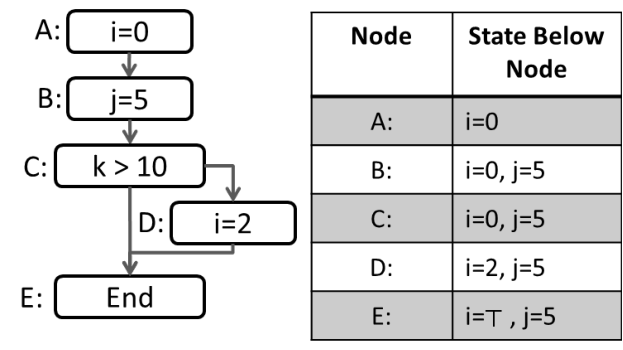
\includegraphics[scale=0.7]{\TutorialExampleDirectory/dfa_cpa}
\caption{Example of a constant propagation analysis.}
\label{Tutorial:dfa_cpa}
\end{figure}

For an intuition about how dataflow analyses work, ~\ref{Tutorial:dfa_cpa} presents an example of a constant propagation analysis. The CFG is on the left and the table on the right shows the fixed-point solution of the abstract state immediately after each node. At each node the abstract application state records for each variable one of the following values: (i) $\bot$, which indicates that the variable is uninitialized, (ii) a specific constant value if the variable may only have this value at node n or (iii) $\top$ which indicates that the variable may have more than one value (i.e., is not representable as a single constant).It shows that immediately after node A it is known that i=0 and similarly after node B, i=0 and j=5. The same is true after node C since it has no side-effects and after the assignment in node D, the state changes to i=2, j=5.  When the two conditional branches meet, the abstract state is the union of the states on both branches: the strongest assertions that are true of both states. Since j has the same value and i has two different values, the abstract state after node E is i=$\top$, j=5.

\begin{figure}
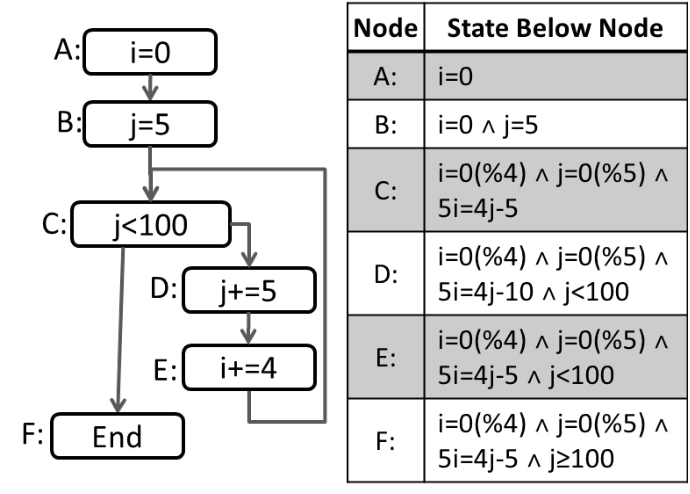
\includegraphics[scale=0.7]{\TutorialExampleDirectory/dfa_ex}
\caption{Example of a dataflow analysis with abstraction of affine constraints.}
\label{Tutorial:dfa_ex}\end{figure}

~\ref{dfa_ex} presents an example with a more complex abstraction: conjunction of linear relationships between variables. At node B the dataflow analysis computes that i=0 and j=5. When this state is propagated through the loop, the analysis discovers that after the first iteration i=4 and j=5. It then computes the meet of i=0 $\wedge$ j=5 and i=4 $\wedge$ j=5, the facts along both paths. Since this abstraction represents linear relationships, the union finds the tightest linear relationships that are true of both input states. It thus infers that i=0 (mod 4), i=0 (mod 5) (i is divisible by 4 and j by 5) and that 5i=4j-5. When this state is propagated again through the body of the loop, these assertions are discovered to be the invariants of this loop and become the fixed-point solution after node C. If they were not invariants, the algorithm would iterate until invariants were found or it reached the abstract state $\top$ which means that no linear constraints are known. Further, since the conditional j\textless100 is also linear, j\textless100 is recorded in the states of the nodes inside the loop and j $\ge$ 100 is recorded at node F after the loop.

\section{ROSE Dataflow Framework}
\label{ROSE_dfa}
ROSE provides a framework for implementing dataflow analyses. It allows users to specify their dataflow analysis by implement the standard dataflow components: (i) an abstraction of the application’s state, (ii) a transfer function that specifies the effects of code on the application state and (iii) a meet operator that combines multiple possible abstract states into one. These are implemented by extending base classes provided by the framework and implementing key virtual methods that correspond to the above functionality. The framework then solves the dataflow equations using the user-provided classes and saves the results at each CFG node. This section describes the functionality provided by the framework and how it can be used to implement analyses. ~\ref{Func_DFA} summarizes the functionality provided by the framework.

\begin{table}
  \centering
  %\tbl{The Functionality of the Dataflow Interface}{
  \scriptsize
  \begin{tabular}{ | p{2cm} | p{2cm} | p{3.5cm} | p{3.5cm} |}
    \hline
    Class & Purpose & Interface & User Responsibilities  \\ \hline
    {\bf Analysis} & Implement Simple CFG passes & Classes {\bf IntraProceduralAnalysis InterProceduralAnalysis} & Extend the classes and implement their {\bf runAnalysis} and {\bf transfer} methods \\ \hline
    {\bf Intra Procedural Dataflow} & Implement intraprocedural dataflow iteration & Classes {\bf IntraFWDataflow} {\bf IntraBWDataflow} & Extend classes and implement {\bf genInitState} and {\bf transfer} methods\\ \hline 
    {\bf Inter Procedural Dataflow} & Implement the inter-procedural dataflow & Classes - {\bf Context Insensitive InterProcedural Dataflow} & Execute on a given instance of {\bf IntraDataflow} \\ \hline
    {\bf Lattice} & Generic interface for abstractions of the application's state & Methods {\bf initialize copy meetUpdate operator== str} & Extend the Lattice class and implement interface methods \\ \hline 
    {\bf Nodestate} & Stores dataflow information of each CFG node & Methods {\bf setLatticeAbove getLatticeAbove deleteLatticeAbove setFact getFact deleteFacts} & Call methods to access dataflow information \\ \hline
    {\bf AstInterface} & Transforms the CFG & Methods {\bf insertBeforeUsing CommaOp, insertAfterUsing CommaOp, replaceWithPattern } & Call methods \\ 
  \hline
  \end{tabular}
%}                                    
  \caption{The Functionality of the Dataflow Interface}
\label{Func_DFA}
\end{table}


\subsection{Call and Control-Flow Graphs}
The ROSE dataflow analysis framework operates on top of the ROSE Call Graph (CG) and Virtual Control-Flow Graph (VCFG). The CG documents the caller/callee relationships between application functions. The VCFG connects SgNodes in the application’s AST to identify the possible execution orders between them. The VCFG is dynamic in that instead of being computing once for the entire application, it computes the outgoing and incoming edges of a given SgNode fresh every time this information is needed. This makes the VCFG very flexible because it automatically responds to changes in the AST with no need for complex adjustments to the graph. 

\subsection{Analyses}
ROSE supports both inter-and intra-procedural analyses. Users implement basic, non-dataflow analyses by extending the {\scriptsize IntraProceduralAnalysis} and {\scriptsize InterProceduralAnalysis} classes. Intra analyses iterate over the CFG of each function, and inter analyses apply intra analyses to individual functions. To implement an analysis an application developer must derive a class from the {\scriptsize IntraProceduralAnalysis} and/or {\scriptsize InterProceduralAnalysis} classes and implement the {\scriptsize runAnalysis} method. Classes {\scriptsize UnstructuredPassInterAnalysis} and {\scriptsize UnstructuredPassIntraAnalysis} {Figure ~\ref{unstruct-ex} provide examples of simple analyses. {\scriptsize UnstructuredPassInterAnalysis} takes as an argument a reference to an {\scriptsize InterProceduralAnalysis} and iterates once through all functions. It applies the {\scriptsize runAnalysis} method of the intra analysis to each function. {\scriptsize UnstructuredPassIntraAnalysis} iterates once through all the CFG nodes in the given function, applying its {\scriptsize visit} method to each node.


\begin{figure}
\centering
\begin{lstlisting}
class UnstructuredPassInterAnalysis : virtual public InterProceduralAnalysis {
  UnstructuredPassInterAnalysis(IntraProceduralAnalysis& intraAnalysis)
  void runAnalysis();
};

class UnstructuredPassIntraAnalysis : virtual public IntraProceduralAnalysis {
   bool runAnalysis(const Function& func, NodeState* state);
   virtual void visit(const Function& func, const DataflowNode& n, 
       NodeState& state)=0;
};  
\end{lstlisting}%
\caption{Example of simple analyses}
\label{unstruct-ex}
\end{figure}

These analyses can be used to implement simple passes through the application’s CFG and serve as the foundation of the dataflow analysis framework. For example, {\scriptsize src/simpleAnalyses/saveDotAnalysis.C} and {\scriptsize src/simpleAnalyses/printAnalysisStates.C} are examples of simple one-pass analyses. {\scriptsize saveDotAnalysis} prints the application’s CFG as a DOT file and {\scriptsize printAnalysisStates} prints the dataflow states of all CFG nodes in the application, which is useful for debugging.

\subsection{Dataflow}
To implement a dataflow analysis in ROSE users must first extend the {\scriptsize Lattice} class to create an abstraction of the application’s state that will be used by the analysis. {\scriptsize Lattices} implement methods such as meet, equality, ordering and operators that allow the {\scriptsize Lattice} to be moved from one lexical scope to another (e.g. from a caller function to the callee). Users then create an intra-procedural analysis by extending the {\scriptsize IntraFWDataflow} to create a forward analysis and from {\scriptsize IntraBWDataflow} to create a backward analysis. Within this class they must implement a function that returns the default abstract state of any given node at the start of the analysis. Further, they implement a {\scriptsize transfer} function that maps the application’s abstract state from before a given CFG node to the state that results from the execution of the node’s expression or statement. Finally, users combine the intra-procedural analysis that they have developed with an inter-procedural analysis of their choice. This analysis will apply the intra-procedural analysis the user has implemented to the application’s functions and resolve the effects of function calls on the application’s abstract state, utilizing the user’s own state abstraction.

For a concrete example, consider how the classical constant-propagation analysis is implemented using ROSE. This analysis uses a simple abstraction of application state, where the abstract state of each variable may be a value the lattice shown in ~\ref{lattice_cpa}

\begin{figure}
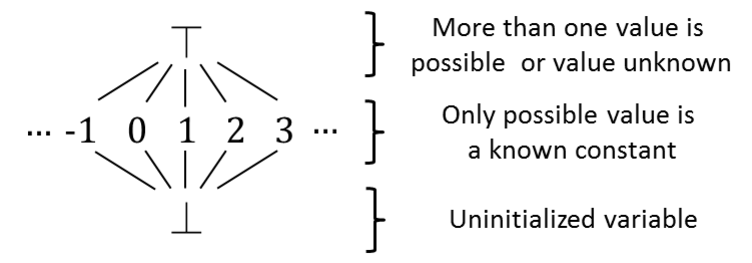
\includegraphics[scale=0.7]{\TutorialExampleDirectory/lattice_cpa}
\caption{Each variable's lattice for constant-propagation analysis}
\label{lattice_cpa}
\end{figure}

The code in below shows a class that implements this lattice. This class derives from the {\scriptsize FiniteLattice} class because the distance between the smallest and largest value in the lattice is finite. Similar functionality is provided for infinite lattices. Its state (lines 4-15) consists of its current level in the lattice as well as its value if the level is {\scriptsize valKnown}. Since the type of {\scriptsize value} is {\scriptsize long}, this abstraction can only represent integral constants. Further, the class has a special {\scriptsize uninitialized} level that means that the object has not yet been used as part of a dataflow analysis. This class implements methods {\scriptsize meetUpdate} (lines 42-65) and the equality operator (lines 68-74) to provide the basic semantics of a lattice. {\scriptsize meetUpdate} computes least upper bound of the constraints in this lattice object and another one, storing the results in this object.If both lattices have the same state, the meet is equal to this state and if they have different states, the meet is $\top$ since the variable represented by the lattice may be set to multiple values on different execution paths. The equality operator determines whether two lattice objects have the same information content. Further, the class implements utility methods that help the dataflow framework manipulate it. The {\scriptsize initialize} method (lines 24-27) ensures the object is ready to be used. Further, two {\scriptsize copy} methods (lines 30-38) make it easy to clone lattice objects. Finally, an {\scriptsize str} method (lines 82-88) simplifies analysis debugging by printing the abstract states at CFG nodes.


%\begin{latexonly}
%   \lstinputlisting{\TutorialExampleDirectory/codesnip_CPA_Lattice.C}
%\end{latexonly}

\begin{frame}
\centering
\begin{lstlisting}
class constPropLat : public FiniteLattice
{
  // The different levels of this object’s lattice
  typedef enum {
    uninitialized=0, // This object is uninitialized
    bottom=1, // No constrains on this object’s value are known
    valKnown=2, // The value of the variable is known (one assignment seen)
    top=3 // This variable may have more than one value
  } latticeLevels;
  
  // The level of this object within its lattice
  latticeLevels level;

  // The value of the variable (if level == valKnown)
  long value;

  nodeConstLattice() { level=uninitialized; }
  
  nodeConstLattice(const nodeConstLattice& that) : 
                              value(that.value), level(that.level) {}

  // Initializes this Lattice to its default state, 
  // if it is not already initialized
  void initialize() {
    if(level == uninitialized)
      level=bottom;
  }
  
  // Returns a copy of this lattice
  Lattice* copy() const { return new nodeConstLattice(*this); }
  
  // Overwrites the state of this Lattice with that of that Lattice
  void copy(Lattice* that) {
    nodeConstLattice* that = dynamic_cast<nodeConstLattice*>(that_arg);
  
    value = that->value;
    level = that->level;
  }

  // Computes the meet of this and that and saves the result in this
  // returns true if this causes this to change and false otherwise
  bool meetUpdate(Lattice* that) {
    // Record this object’s original state to enable change detection
    unsigned long  oldValue = value;
    latticeLevels oldLevel = level;
    
    // Cast that into a nodeConstLattice and abort if this is not possible    
    nodeConstLattice* that = dynamic_cast<nodeConstLattice*>(that_arg);
    ROSE_ASSERT(that);

    // If that is at a higher lattice level than this, the variable must have 
    // multiple possible value on different execution paths
    if(that->level > level) level = top;
    // If both are at the same level
    else if(that->level == level) {
      // If lattices correspond to different values of the variable
      if(level == valKnown && value != that->value)
        level = top; // The union of both these facts is top
    }
    // Otherwise, this lattice doesn’t change
    
    // Return whether this object was modified
    return (oldValID != valID) ||
           (oldLevel != level);
  }
  
  // Equality Operator
  bool operator==(Lattice* that_arg) { 
    // Cast that into a nodeConstLattice and abort if this is not possible    
    nodeConstLattice* that = dynamic_cast<nodeConstLattice*>(that_arg);
    ROSE_ASSERT(that);
    
    return level==that->level && (level!=valKnown || value==that->value);
  }

  // Returns a string representation of this object (this function is 
  // required to simplify debugging)
  string str(string indent="") { … }

  // Sets the state of this lattice to the given value. Returns true if this 
  // causes the lattice's state to change, false otherwise
  bool set(long value)
  {
    bool modified = this->level != valKnown || this->value != value;
    this-> value = value;
    level = valKnown;
    return modified;
  }
}; 
\end{lstlisting}%
\label{unstruct-ex}
\end{frame}


The second step in implementing constant propagation is to provide a class that implements the dataflow analysis itself. This is done by extending the {\scriptsize IntraFWDataflow} class, which implements forward intra-procedural analyses and implementing the {\scriptsize genInitState} and {\scriptsize transfer} methods, described below.

\begin{frame}
\centering
\begin{lstlisting}
class constPropAnalysis : public IntraFWDataflow
{
  constPropAnalysis (): IntraFWDataflow() { }

  // Generates the initial lattice state for the given dataflow node, in the 
  // given function, with the given NodeState
  void genInitState(const Function& func, const DataflowNode& n, 
                    const NodeState& state, vector<Lattice*>& initLattices, 
                    vector<NodeFact*>& initFacts);

  // The transfer function that is applied to every node in the CFG
  // n - The dataflow node that is being processed
  // state - The NodeState object that describes the state of the node, as  
  //         established by earlier analysis passes
  // dfInfo - The Lattices that this transfer function operates on. The 
  //          function takes these lattices as input and overwrites them with 
  //          the result of the transfer.
  // Returns true if any of the input lattices changed as a result of the
  //    transfer function and false otherwise.
  bool transfer(const Function& func, const DataflowNode& n, 
              NodeState& state, const vector<Lattice*>& dfInfo);
}
\end{lstlisting}%
\end{frame}

The {\scriptsize constPropAnalysis} implementation of method {\scriptsize genInitState} creates a lattice (lines 5-7) that maintains the initial abstract state of the application at CFG node {\scriptsize n}. This lattice is an instance of the utility class {\scriptsize FiniteVarsExprsProductLattice}, which creates one copy of {\scriptsize constPropLat} for each variable that is live at node {\scriptsize n}. Since it is a product of lattices, this class is also a lattice with well-defined meet and equality operators based on the operators of its constituent lattices. The dataflow framework provides an identical class for infinite lattices as well as a generic ProductLattice class for arbitrary products of lattices. The function then adds (line 4) the lattice to vector initLattices, which is read by the dataflow framework. This function can also specify one or more facts that the framework will maintain at each node. These facts are not subject to dataflow iteration and can be used to maintain information that is useful independently of the current dataflow state.
 

\begin{frame}
\centering
\begin{lstlisting}
void constPropAnalysis::genInitState(const Function& func, 
              const DataflowNode& n, const NodeState& state,
              vector<Lattice*>& initLattices, vector<NodeFact*>& initFacts) {
  initLattices.push_back(
          new FiniteVarsExprsProductLattice(true, false,  
                                            new constPropLat(), 
                                            NULL, func, n, state));
}
\end{lstlisting}%
\end{frame}

The {\scriptsize transfer} method maps the abstract state before the CFG node n to the state that results from its execution. It begins by accessing the application’s abstract state above node n from the {\scriptsize dfInfo} argument (lines 6-7) . This is the vector of lattices created by {\scriptsize genInitState} for node {\scriptsize n}. It can also be obtained from the {\scriptsize state} object, which maintains the state of the lattices both below and above each node, as well as the facts at each node. The function then initializes all the {\scriptsize constPropLats} in the product lattice (10-13) and advances to analyze the effects of the current node on the abstract state.

Lines 16-127 show how the transfer function operates on different types of {\scriptsize SgNodes}. This code leverages a key feature of how ROSE represents the application’s structure. Since ROSE focuses on source-to-source transformations that minimize the changes in the application’s source code, all analyses must work on the original AST and cannot perform large normalization passes such as transforming the application into SSA form. Since it is difficult to implement complex analyses on top of the AST, we have developed an ``on-demand'' normalization that significantly simplifies the analysis development without changing the AST. Working with AST is difficult because AST sub-trees that describe the structure of expressions are complex and difficult to parse (e.g. consider analyzing all the side-effects of a=b=foo(c=d)). As such, our framework treats every SgExpression that does not correspond to an actual memory object as if it produces a temporary object that is read by its parent {\scriptsize SgExpression}. For example, in the {\scriptsize SgExpression} a=(b=c*5+d), {\scriptsize SgIntVal} 5 produces a temporary variable that is consumed by {\scriptsize SgMultiplyOp c*5. SgVarRefExp c} produces a real application variable, which is also consumed by the {\scriptsize SgMultiplyOp}. The SgMultiplyOp in turn produces a temporary variable that is consumed by {\scriptsize SgAddOp c*5+d}, which produces a temporary variable that is consumed by {\scriptsize SgAssignOp b=c*5+d}, the result of which is consumed by {\scriptsize SgAssignOp a=(b=c*5+d)}. The use of these temporary variables makes it possible for user analyses to focus on just the effects of individual AST nodes without having to analyze sub-trees of the AST. Section~\ref{transfer_analyses} discusses how this on-demand normalization in maintained when updating to the AST. 

The effects of integral constants (e.g. {\scriptsize SgIntVal} or {\scriptsize SgLongLongIntVal}) are transferred on lines 16-31. On line 20 the analysis calls function SgExpr2Var to convert the {\scriptsize SgExpression} into a {\scriptsize varID}, which is an abstract representation of the memory object (either a real or temporary variable) denoted by the {\scriptsize SgExpression}. On line 21 it queries the {\scriptsize FiniteVarsExprsProductLattice} prod with this {\scriptsize varID} to get the {\scriptsize constPropLat} associated with this memory object. If this variable is live (a non-NULL lattice is returned), on lines 26-28 it sets the lattice object to be at level {\scriptsize valKnown} and sets the value to be equal to the constant represented by the {\scriptsize SgExpression}.

 The same logic is used for non-integral constants on lines 33-40. However, since our abstraction cannot represent such constants, their lattices are set to $\top$. Lines 44-60 manage assignments and the lattices of the left-hand-side expression and the assignment {\scriptsize SgAssignOp} itself are set to be equal to the lattice of the right-hand-side expression. The code for variable declaration (lines 63-81) and initialization (lines 84-98) are similar in that the lattice of the right-hand-side is copied to the lattice of the initialized variable. Finally, lines 101-127 focus on arithmetic operations. If the lattices of the left- and right-hand-side expressions are both at levels {\scriptsize valKnown},the operation is performed immediately by the analysis on their statically known values and the result is stored in the lattices of the left-hand-side expression and the {\scriptsize SgExpression} itself. Finally, on line 129 the function returns the {\scriptsize modified} variable, which keeps track of whether the state of the downstream lattices has changed. Since these lattices are inputs to other {\scriptsize SgExpressions}, this informs the dataflow framework whether it needs to analyze how these lattices are transferred by those expressions.   


\begin{frame}
\centering
\begin{lstlisting}
bool constPropAnalysis::transfer(const Function& func, 
                       const DataflowNode& n, 
                       NodeState& state, const vector<Lattice*>& dfInfo) {
  bool modified=false;
  // Get the lattice object
  FiniteVarsExprsProductLattice* prodLat = 
            dynamic_cast<FiniteVarsExprsProductLattice*>(*(dfInfo.begin()));

  // Make sure that all the non-constant Lattices are initialized
  const vector<Lattice*>& lattices = prodLat->getLattices();
  for(vector<Lattice*>::const_iterator it = lattices.begin(); 
      it!=lattices.end(); it++)
    (dynamic_cast<nodeConstLattice*>(*it))->initialize();

  // Integral Numeric Constants
  if(isSgLongLongIntVal(n.getNode())  || 
    // Other types of integral constants 
    ...) {
    // Memory object and lattice of the expression’s result
    varID res = SgExpr2Var(isSgExpression(n.getNode()));
    constPropLat* resLat = dynamic_cast<constPropLat*>(
                                                prodLat->getVarLattice(res));

    // If the result expression is live
    if(resLat) {
      if(isSgLongLongIntVal(n.getNode()))
        modified = resLat->set(isSgLongLongIntVal(n.getNode())->get_value()) 
                   || modified;
      // Same for other types of integral constants 
      ...
    }
  // Non-integral Constants
  } else if(isSgValueExp(n.getNode())) {
    // Memory object and lattice of the expression’s result
    varID res = SgExpr2Var(isSgExpression(n.getNode()));
    constPropLat* resLat = dynamic_cast<constPropLat*>(
                                                prodLat->getVarLattice(res));
    // If the result expression is live, set it to top since we only work 
    // with integral constants
    if(resLat) modified = resLat->setTop() || modified;

  // Plain assignment: lhs = rhs
  } else if(isSgAssignOp(n.getNode())) {
    // Memory objects denoted by the expression’s left- and right-hand   
    // sides as well as the SgAssignOp itself
    varID lhs = SgExpr2Var(isSgAssignOp(n.getNode())->get_lhs_operand());
    varID rhs = SgExpr2Var(isSgAssignOp(n.getNode())->get_rhs_operand());
    varID res = SgExpr2Var(isSgExpression(n.getNode()));

    // The lattices associated the three memory objects
    constPropLat* resLat = 
            dynamic_cast<constPropLat*>(prodLat->getVarLattice(res));
    constPropLat* lhsLat = 
            dynamic_cast<constPropLat*>(prodLat->getVarLattice(lhs));
    constPropLat* rhsLat = 
            dynamic_cast<constPropLat*>(prodLat->getVarLattice(rhs));

    // If the lhs and/or the SgAssignOp are live, copy lattice from the rhs
    if(lhsLat){ lhsLat->copy(rhsLat); modified = true; }    
    if(resLat){ resLat->copy(rhsLat); modified = true; }    

  // Variable Declaration
  } else if(isSgInitializedName(n.getNode())) {
    varID var(isSgInitializedName(n.getNode()));
    constPropLat* varLat = dynamic_cast<constPropLat*>(
                                               prodLat->getVarLattice(var));

    // If this variable is live
    if(varLat) {
      // If there was no initializer, initialize its lattice to Bottom
      if(initName->get_initializer()==NULL)
        modified = varLat->setBot() || modified;
      // Otherwise, copy the lattice of the initializer to the variable
      else {
        varID init = SgExpr2Var(
                        isSgInitializedName(n.getNode())->get_initializer());
        ConstPropLat* initLat = dynamic_cast<ConstPropLat*>(
                                               prodLat->getVarLattice(init));
        if(initLat) { varLat->copy(initLat); modified = true; }
      }
    }

  // Initializer for a variable
  } else if(isSgAssignInitializer(n.getNode())) {
    // Memory objects of the initialized variable and the 
    // initialization expression
    varID res = SgExpr2Var(isSgAssignInitializer(n.getNode()));
    varID asgn = SgExpr2Var(isSgAssignInitializer(
                                         n.getNode())->get_operand());

    // The lattices associated both memory objects
    constPropLat* resLat = 
            dynamic_cast<constPropLat*>(prodLat->getVarLattice(res));
    constPropLat* asgnLat = 
            dynamic_cast<constPropLat*>(prodLat->getVarLattice(asgn));

    // If the variable is live, copy lattice from the assignment
    if(resLat){ resLat->copy(asgnLat); modified = true; }

  // += Arithmetic Operation
  } else if(isSgPlusAssignOp(n.getNode())) {
    // Memory objects denoted by the expression’s left- and right-hand   
    // sides as well as the SgAssignOp itself
    varID lhs = SgExpr2Var(isSgAssignOp(n.getNode())->get_lhs_operand());
    varID rhs = SgExpr2Var(isSgAssignOp(n.getNode())->get_rhs_operand());
    varID res = SgExpr2Var(isSgExpression(n.getNode()));

    // The lattices associated the three memory objects
    constPropLat* resLat = 
            dynamic_cast<constPropLat*>(prodLat->getVarLattice(res));
    constPropLat* lhsLat = 
            dynamic_cast<constPropLat*>(prodLat->getVarLattice(lhs));
    constPropLat* rhsLat = 
            dynamic_cast<constPropLat*>(prodLat->getVarLattice(rhs));

    // If the lhs and/or the SgAssignOp are live and we know both their 
    // values of the value of the rhs expression, set their lattice to be the     
    // sum of the two.
    if(lhsLat && lhsLat->level==constPropLat::valKnown && 
       rhsLat->level==constPropLat::valKnown)
    { modified = lhsLat->set(lhsLat->value + rhsLat->value) || modified; }
    if(resLat && resLat->level==constPropLat::valKnown && 
       rhsLat->level==constPropLat::valKnown)
    { modified = resLat->set(resLat->value + rhsLat->value) || modified; }
  } 
  // Same for other arithmetic operations
  ...

  return modified;
}
\end{lstlisting}%
\end{frame}
Once the intra-procedural analysis has been implemented, it can be executed on the application by combining it with an inter-procedural analysis. Currently two such analyses are implemented. {\scriptsize ContextInsensitiveInterProceduralDataflow} implements a basic context-insensitive analysis that propagates abstract state from callers to callees but does not differentiate between different call sites of the same function. As such, it is sensitive to inter-procedural data flows but can be imprecise because it takes into account control flows that are actually impossible, such as entering a function from one call site but returning to another. The code below provides an example of how this analysis is used to create an inter-procedural constant propagation analysis. The dataflow framework is initialized on line 6 and the application’s call graph is built on lines 9-11. The intra-procedural analysis object is created on line 17 and the context-insensitive inter-procedural analysis is created on line 20. The user passes into its constructor references to their intra-procedural analysis and the call graph. Finally, on line 23 the user applies the full inter-procedural analysis to the entire application. 
 
\begin{frame}
\centering
\begin{lstlisting}
int main( int argc, char * argv[] )  {
  // Build the AST used by ROSE
  SgProject* project = frontend(argc,argv);
  
  // Initialize the ROSE dataflow framework
  initAnalysis(project);

  // Build the call graph
  CallGraphBuilder cgb(project);
  cgb.buildCallGraph();
  SgIncidenceDirectedGraph* graph = cgb.getGraph(); 

  // Set the debug level to print the progress of the dataflow analysis
  analysisDebugLevel = 1;
  
  // Create the intra-procedural constant propagation analysis
  constPropAnalysis cp(project);

  // Create the inter-procedural analysis for intra-analysis cp
  ContextInsensitiveInterProceduralDataflow inter_cp(&cp, graph);

  // Run inter-procedural constant propagation on the entire application
  inter_cp.runAnalysis();
}
\end{lstlisting}
\end{frame}

To simplify debugging the framework also provides the {\scriptsize UnstructuredPassInterDataflow} analysis, which simply applies the user’s intra-procedural analysis on each function within the application. While this produces globally incorrect results, it simplifies debugging analyses on individual functions. 

\subsection{Transferring Information Between Analyses}
\label{transfer_analyses}
Since in practice users need to implement multiple analyses where one depends on the results of another, the ROSE dataflow framework maintains the results of all analyses at each CFG nodes and makes it easy for analyses to access this data. The lattices and facts of a given CFG node are stored in its associated {\scriptsize NodeState} object. The data produced by an analysis can be retrieved by using its pointer, as shown in the example below.

This code shows analysis {\scriptsize exAnalysis}, which takes in its constructor a pointer to the {\scriptsize constPropAnalysis} described above (lines 4-5). Inside its transfer function this analysis calls the {\scriptsize getLatticeBelow} method of its argument state (instance of the {\scriptsize NodeState} class) to get the lattice associated with {\scriptsize constPropAnalysis} that has index 0 (lines 11-13). It then gets the {\scriptsize constPropLat} of any variable it cares about and make analysis decisions based on what is statically known about its state.

\begin{frame}
\centering
\begin{lstlisting}
class exAnalysis {
  // Class maintains a pointer to the constant propagation analysis to make 
  // it possible to access its results
  constPropAnalysis& cpAnalysis;
  exAnalysis(constPropAnalysis* cpAnalysis) : cpAnalysis (cpAnalysis) {}

  bool transfer(const Function& func, const DataflowNode& n, 
                NodeState& state, const vector<Lattice*>& dfInfo) {
    // Get the Lattices computed by the constant propagation analysis for the 
    // current CFG node
    FiniteVarsExprsProductLattice* prodLat = 
               dynamic_cast<FiniteVarsExprsProductLattice*>(
                                      state->getLatticeBelow(cpAnalysis, 0));

    // Some application variable of interest
    varID var = ...;

    // The constPropLat of this variable
    constPropLat varCPLat = dynamic_cast<constPropLat*>(
                                                prodLat->getVarLattice(res));

    // Analyze differently depending on what is known about the 
    // variable’s value 
    if(varCPLat) 
      if(varCPLat->level == constPropLat::bottom) {
        ...
      } else if(varCPLat->level == constPropLat::valKnown) {
        ...
      } else if(varCPLat->level == constPropLat::top) {
        ...
      }
  }
  ...
};
\end{lstlisting}
\end{frame}

The code below shows the full functionality of the {\scriptsize NodeState} class. . Lines 5-16 show the functions to set, get and delete the lattices above and below the associated CFG node.  Lines 20-26 provide the same functionality for facts. The {\scriptsize str} method on line 20 returns a string representation of the lattices and facts associated with the CFG node, which is very useful for debugging. Lines 37-50 show the object’s static methods. The {\scriptsize getNodeState} method on line 37 returns the {\scriptsize NodeState} object of a given CFG node. Since the ROSE virtual CFG can have multiple CFG nodes for the same AST node, this method requires an additional index argument to identify the node in question. Finally, method copyLattices\_aEQa and related methods (lines 39-50) copy lattice information from above a CFG node to below it and vice versa, from one node to another or from one analysis at a given node to another analysis at the same node.  

\begin{frame}
\centering
\begin{lstlisting}
class NodeState
{
  // Sets the lattices above/below this node for the given analysis to the   
  // given lattice vector
  void setLatticeAbove(const Analysis* analysis, vector<Lattice*>& lattices);
  void setLatticeBelow(const Analysis* analysis, vector<Lattice*>& lattices);
  
  // Returns the lattice latticeName generated by the given analysis from 
  // above/below the node
  Lattice* getLatticeAbove(const Analysis* analysis, int latticeName) const;
  Lattice* getLatticeBelow(const Analysis* analysis, int latticeName) const;
  
  // Deletes all lattices above/below this node that are associated with the 
  // given analysis
  void deleteLatticeAbove(const Analysis* analysis);
  void deleteLatticeBelow(const Analysis* analysis);
  
  // Sets the facts at this node for the given analysis to the given 
  // fact vector
  void setFacts(const Analysis* analysis, const vector<NodeFact*>& newFacts);
  
  // Returns the given fact, owned by the given analysis
  NodeFact* getFact(const Analysis* analysis, int factName) const ;
  
  // Deletes all facts at this node associated with the given analysis
  void deleteFacts(const Analysis* analysis);

  // Returns a string representation of all the lattices and facts 
  // associated with the CFG node
  string str(Analysis* analysis, string indent) const;

  // --- Static Methods --- 
  // Returns the NodeState object associated with the given dataflow node
  // index is used when multiple NodeState objects are associated with a 
  // given node
  // (ex: SgFunctionCallExp has 3 NodeStates: entry, function body, exit)
  static NodeState* getNodeState(const DataflowNode& n, int index=0);
    
  // Copies from's above lattices for the given analysis to to's above 
  // lattices for the same analysis
  static void copyLattices_aEQa(Analysis* analysis, NodeState& to, const 
                                NodeState& from);
  
  // Copies from's above lattices for analysisA to to's above lattices for 
  // analysisB
  static void copyLattices_aEQa(Analysis* analysisA, NodeState& to, 
                                Analysis* analysisB, const NodeState& from);
  
  // Similar methods for copying in different permutations
  ...
};
\end{lstlisting}
\end{frame}

\subsection{CFG Transformations}
ROSE makes it easy to modify the application’s AST as a result of dataflow analyses. The dataflow framework maintains an on-demand normal form, where analyses can focus on the actions of individual SgNodes and ignore how they are arranged within the AST. ROSE maintains this abstraction by providing an API that inserts new SgExpressions into the application’s CFG, making all the needed changes in the AST to make sure that the correct control flow is maintained. 


\begin{figure}
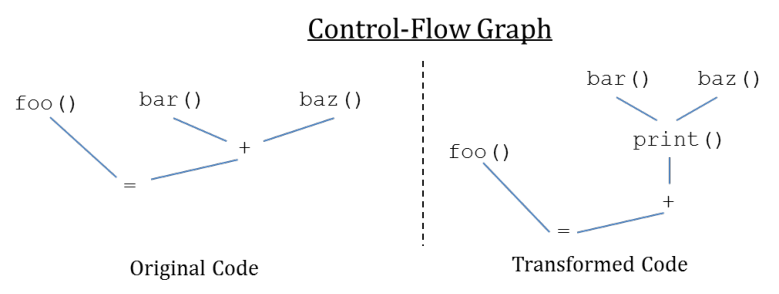
\includegraphics[scale=0.7]{\TutorialExampleDirectory/transformation_cfg.pdf}
\caption{Example of Transformation on the CFG}
\label{tr_cfg}
\end{figure}

To get the intuition of this functionality consider the expression {\scriptsize foo()=(bar()+baz())}. Suppose the user has decided based on the dataflow state before the {\scriptsize SgAddOp +} that it they want to add a call to function {\scriptsize print} immediately before it. From the perspective of the CFG, this is a simple and well-defined operation, as shown at the top of Figure 4. The side-effects of the calls to {\scriptsize bar} and {\scriptsize baz} must complete before the call to print and the side-effects of print must complete before the execution of the + operation. The call to {\scriptsize foo} is not well-ordered relative print or the other operations by the structure of the CFG.

Unfortunately, it is difficult to implement these semantics in the context of the AST because (i) there is no way to add a function call to an {\scriptsize SgAddOp} and (ii) because in C++ the sequence points required by the above semantics (some side-effects much complete before others) are provided by a few specific constructs such as statement boundaries and the comma operator. As such, the transformation requires the complex set of AST changes shown in the Figure 5. We must create temporary variables to hold the results of the calls to bar and baz. We then transform the original {\scriptsize SgAddOp} into a longer {\scriptsize SgCommaOpExp}, where we first call {\scriptsize bar} and {\scriptsize baz}, saving their results into the temporary variables, then call print and finally perform the addition. The result of the addition is the result of the entire comma expression, so this transformation correctly enforces the semantics of the desired transformation.


\begin{figure}
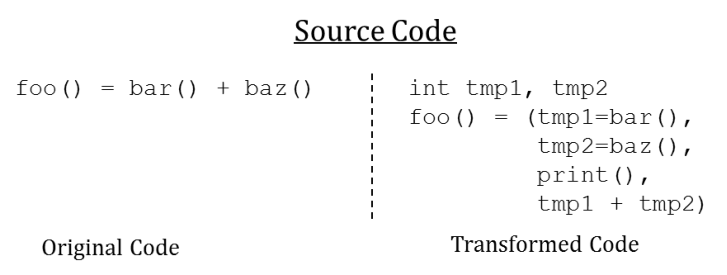
\includegraphics[scale=0.7]{\TutorialExampleDirectory/transformation_srcode.pdf}
\caption{Example of the Transformation on the Source Code}
\label{tr_srcode}
\end{figure}

ROSE provides the three functions to make it easy to insert expressions into the CFG. Functions {\scriptsize insertBeforeUsingCommaOp} and {\scriptsize insertAfterUsingCommaOp} insert {\scriptsize SgExpressions} before or after existing {\scriptsize SgExpressions} using a generalization of the transformation described in Figure ~\ref{tr_srcode}. 

\begin{frame}
\centering
\begin{lstlisting}
// Insert an expression (new_exp) before another expression (anchor_exp) has 
// possible side effects, without changing the original semantics. This is 
// achieved by using a comma operator: (new_exp, anchor_exp). The comma 
// operator is returned.
SgCommaOpExp *insertBeforeUsingCommaOp(SgExpression* new_exp, 
                                       SgExpression* anchor_exp);
// Insert an expression (new_exp) after another expression (anchor_exp) has 
// possible side effects, without changing the original semantics. This is 
// done by using two comma operators:  
//     type T1; ... ((T1 = anchor_exp, new_exp),T1) )... , 
// where T1 is a temp variable saving the possible side effect of anchor_exp. 
// The top level comma op exp is returned. The reference to T1 in T1 = 
// anchor_exp is saved in temp_ref.
SgCommaOpExp *insertAfterUsingCommaOp(SgExpression* new_exp, 
                    SgExpression* anchor_exp, SgStatement** temp_decl = NULL, 
                    SgVarRefExp** temp_ref = NULL);
\end{lstlisting}%
\label{insert-ex}
\end{frame}

Function replaceWithPattern (Figure~\ref{rep}) replaces one SgExpression with another. However, since the original expression may still be valuable, it allows the original expression to be included at one or more locations inside the new expression that contain nodes of type SgVariantExpression. 


\begin{frame}
\centering
\begin{lstlisting}
// Replace an anchor node with a specified pattern subtree with optional 
// SgVariantExpression. All SgVariantExpression in the pattern will be 
// replaced with copies of the anchor node.
SgNode* replaceWithPattern (SgNode * anchor, SgNode* new_pattern);
\end{lstlisting}%
\label{rep}
\end{frame}

An example of this transformation is shown Figure~\ref{cfg-srcode}, where the original code is the same as in the example above and the {\scriptsize new\_pattern} expression is a single {\scriptsize SgMultOp} where the arguments are both {\scriptsize SgVariantExpressions}. The result of the transformation is that the original {\scriptsize SgAddOp} is replaced with a multiplication the arguments of which are copies of the {\scriptsize SgAddOp: (bar()+baz())*(bar()+baz())}.


\begin{figure}
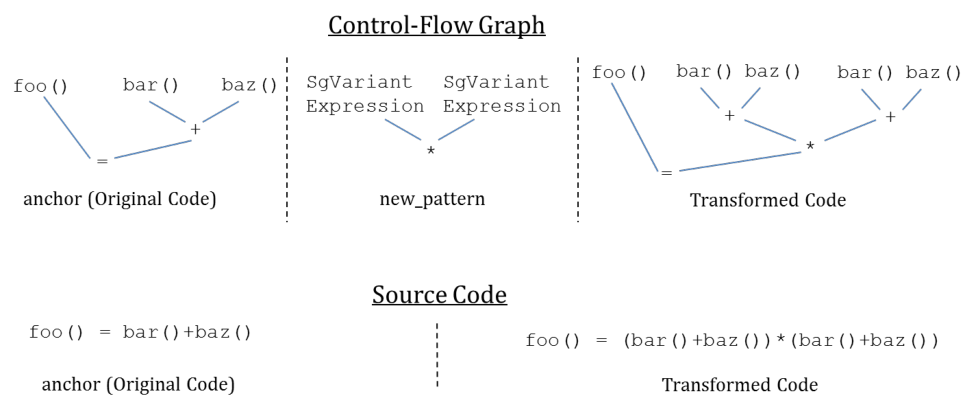
\includegraphics[scale=0.7]{\TutorialExampleDirectory/code_replacement_transformation.pdf}
\caption{Code Replacement Transformation}
\label{cfg-srcode}
\end{figure}


\chapter{Recognizing Loops}

   Figures~\ref{Tutorial:exampleLoopRecognition-part1} and
\ref{Tutorial:exampleLoopRecognition-part2} show a translator which
reads an application and gathers a list of loop nests.  At the end of the traversal it
reports information about each loop nest, including the function where it occurred
and the depth of the loop nest.

\fixme{This example program is unfinished. It will output a list of objects representing
       information about perfectly nested loops.}

\begin{figure}[!h]
{\indent
{\mySmallestFontSize


% Do this when processing latex to generate non-html (not using latex2html)
\begin{latexonly}
   \lstinputlisting{\TutorialExampleBuildDirectory/loopRecognition.aa}
\end{latexonly}

% Do this when processing latex to build html (using latex2html)
\begin{htmlonly}
   \verbatiminput{\TutorialExampleDirectory/loopRecognition.C}
\end{htmlonly}

% end of scope in font size
}
% End of scope in indentation
}
\caption{Example source code showing loop recognition (part 1).}
\label{Tutorial:exampleLoopRecognition-part1}
\end{figure}

\begin{figure}[!h]
{\indent
{\mySmallestFontSize


% Do this when processing latex to generate non-html (not using latex2html)
\begin{latexonly}
   \lstinputlisting{\TutorialExampleBuildDirectory/loopRecognition.ab}
\end{latexonly}

% Do this when processing latex to build html (using latex2html)
\begin{htmlonly}
   \verbatiminput{\TutorialExampleDirectory/loopRecognition.C}
\end{htmlonly}

% end of scope in font size
}
% End of scope in indentation
}
\caption{Example source code showing loop recognition (part 2).}
\label{Tutorial:exampleLoopRecognition-part2}
\end{figure}


   Using this translator we can compile the code shown in 
figure~\ref{Tutorial:exampleInputCode_LoopRecognition}.  The 
output is shown in figure~\ref{Tutorial:exampleOutput_LoopRecognition}.

\begin{figure}[!h]
{\indent
{\mySmallFontSize


% Do this when processing latex to generate non-html (not using latex2html)
\begin{latexonly}
   \lstinputlisting{\TutorialExampleDirectory/inputCode_LoopRecognition.C}
\end{latexonly}

% Do this when processing latex to build html (using latex2html)
\begin{htmlonly}
   \verbatiminput{\TutorialExampleDirectory/inputCode_LoopRecognition.C}
\end{htmlonly}

% end of scope in font size
}
% End of scope in indentation
}
\caption{Example source code used as input to loop recognition processor.}
\label{Tutorial:exampleInputCode_LoopRecognition}
\end{figure}

\begin{figure}[!h]
{\indent
{\mySmallFontSize


% Do this when processing latex to generate non-html (not using latex2html)
\begin{latexonly}
   \lstinputlisting{\TutorialExampleBuildDirectory/loopRecognition.out}
\end{latexonly}

% Do this when processing latex to build html (using latex2html)
\begin{htmlonly}
   \verbatiminput{\TutorialExampleBuildDirectory/loopRecognition.out}
\end{htmlonly}

% end of scope in font size
}
% End of scope in indentation
}
\caption{Output of input to loop recognition processor.}
\label{Tutorial:exampleOutput_LoopRecognition}
\end{figure}




\chapter{Virtual CFG}

The ROSE virtual control flow graph interface provides a higher level of
detail than ROSE's other control flow graph interfaces.  It expresses
control flow even within expressions, and handles short-circuited logical
and conditional operators properly\footnote{It assumes operands of
expressions are computed in left-to-right order, unlike the actual language
semantics, however.}.  The interface is referred to as ``virtual'' because
no explicit graph is ever created: only the particular CFG nodes and edges
used in a given program ever exist.  CFG nodes and edges are value classes
(they are copied around by value, reducing the need for explicit memory
management).

A CFG node consists of two components: an AST node pointer, and an index of
a particular CFG node within that AST node.  There can be several CFG nodes
corresponding to a given AST node, and thus the AST node pointers cannot be
used to index CFG nodes.  The particular index values for the different AST
node types are explained in Section~\ref{cfg_index_values}.

\section{CFGNode Index values}
\label{cfg_index_values}
To facilitate traversal and represent sufficient details,
each eligible ROSE AST node (expression, statement and SgInitializedName)
has several corresponding CFGNodes in virtual CFG. 
These CFGNodes have indices from 0 to n. CFGNode of index value of 0 is 
used to represent the beginning CFG node for an AST node, while the CFGNode
of index n is the end CFGNode for the AST node.
The
beginning node represents the point in the control flow immediately before
the construct starts to execute, and the ending node represents the point
immediately after the construct has finished executing.  Note that these
two nodes do not dominate the other CFG nodes in the construct due to
\lstinline{goto} statements and labels.

Reimplementation of {\textit SgNode::cfgIndexForEnd()} returns the index value for n of each
eligible SgNode type. See source file
\textit{src/frontend/SageIII/virtualCFG/memberFunctions.C} for valid index
values for each type of eligible SgNode. 


\section{Important functions}

The main body of the virtual CFG interface is in \lstinline{virtualCFG.h};
the source code is in \lstinline{src/frontend/SageIII/virtualCFG/} and is
linked into \lstinline{librose}.  The filtered CFG interface explained
below is in \lstinline{filteredCFG.h}, and functions for converting the CFG
to a graph in Dot format are in \lstinline{cfgToDot.h}.

Two functions provide the basic way of converting from AST nodes to CFG
nodes.  Each \lstinline{SgNode} has two methods,
\lstinline{cfgForBeginning()} and \lstinline{cfgForEnd()}, to generate the
corresponding beginning and end CFG nodes, respectively.  
These functions require that the AST node is
either an expression, a statement, or a \lstinline{SgInitializedName}.  
\subsection{Node methods}

\begin{itemize}
\item \lstinline{CFGNode(SgNode* node, unsigned int index)}: Build a CFG
node from the given AST node and index.  Valid index values are in
Section~\ref{cfg_index_values}. 
\item \lstinline{toString()}: Produce a string representing the information
in the node.
\item \lstinline{toStringForDebugging()}: Similar, but with more internal
debugging information.
\item \lstinline{id()}: A C identifier representing the node.
\item \lstinline{getNode()}: Get the underlying AST node.
\item \lstinline{getIndex()}: Get the index (as explained in
Section~\ref{cfg_index_values}) for this CFG node within its underlying AST
node.
\item \lstinline{outEdges()}: Return a vector of outgoing CFG edges from
this node. This function internally calls 
\lstinline{cfgOutEdges(unsigned int idx)} to
generate out edges for each CFGNode of a given index value. 
\item \lstinline{inEdges()}: Return a vector of CFG edges coming into this
node (note that the sources and targets of the edges are not reversed, and
so each in edge has its target as the current node). This function
internally calls \lstinline{cfgInEdges(unsigned int idx) } to generate
in edges for each CFGNode of a given index value. 
\item \lstinline{isInteresting()}: See
Section~\ref{interesting_node_filter}.
\item Nodes are also comparable using the operators \lstinline{==},
\lstinline{!=}, and \lstinline{<}.
\end{itemize}

\subsection{Edge methods}

\begin{itemize}
\item \lstinline{toString()}: Produce a string representing the information
      in the node.
\item \lstinline{toStringForDebugging()}: Similar, but with more internal
      debugging information.
\item \lstinline{id()}: A C identifier representing the node.
\item \lstinline{source()}: The starting CFG node for this edge.
\item \lstinline{target()}: The ending CFG node for this edge.
\item \lstinline{condition()}: When there are multiple CFG edges from the
      same starting node, each of them is taken under certain conditions.  The
\lstinline{condition()} method returns the condition, of type
\lstinline{EdgeConditionKind}.  The possible return values are:
  \begin{itemize}
  \item \lstinline{eckUnconditional}: An edge that is always taken.
  \item \lstinline{eckTrue}: True case of a two-way branch (either an
                             \lstinline{if} statement or a loop
  \item \lstinline{eckFalse}: False case of a two-way branch
  \item \lstinline{eckCaseLabel}: Case label in a \lstinline{switch} statement (key is given by \lstinline{caseLabel()})
  \item \lstinline{eckDefault}: Default label of a \lstinline{switch} statement
  \item \lstinline{eckDoConditionPassed}: Enter Fortran \lstinline{do} loop body
  \item \lstinline{eckDoConditionFailed}: Fortran \lstinline{do} loop finished
  \item \lstinline{eckForallIndicesInRange}: Start testing \lstinline{forall} mask
  \item \lstinline{eckForallIndicesNotInRange}: End of \lstinline{forall} loop
  \item \lstinline{eckComputedGotoCaseLabel}: Case in computed \lstinline{goto} -- number needs to be computed separately
  \item \lstinline{eckArithmeticIfLess}: Edge for the arithmetic \lstinline{if} expression being less than zero
  \item \lstinline{eckArithmeticIfEqual}: Edge for the arithmetic \lstinline{if} expression being equal to zero
  \item \lstinline{eckArithmeticIfGreater}: Edge for the arithmetic \lstinline{if} expression being greater than zero
  \end{itemize}
\item \lstinline{caseLabel()}: For an edge with condition
      \lstinline{eckCaseLabel}, an expression representing the key for the case
      label.
\item \lstinline{computedGotoCaseIndex()}: The index of this edge's case
      within a Fortran computed \lstinline{goto} (an edge of kind
      \lstinline{eckComputedGotoCaseLabel}).
\item \lstinline{conditionBasedOn()}: The test expression or
      \lstinline{switch} expression that is tested by this edge.
\item \lstinline{scopesBeingExited()}, \lstinline{scopesBeingEntered()}:
      Variables leaving and entering scope during this edge.  This information
      has not been extensively verified, and should not be relied upon.
\item Edges can also be compared using the operators \lstinline{==} and
      \lstinline{!=}.  They are not ordered to avoid dependencies on pointer
      comparison on different computers.
\end{itemize}

\section{Drawing a graph of the CFG}

Fig.~\ref{Tutorial:BuildVirtualCFG1} shows a translator to dump 
full (debug) virtual control flow graphs for all functions within input
source files. It also dumps a simplified version (interesting) version of 
virtual control flow graphs. A standalone tool named \textit{virtualCFG} is
installed under \textit{ROSE\_INSTALL\_TREE/bin} for users to generate both
debug and interesting dot files of virtual CFGs. 

%---------------------------------------------------------------------------
\begin{figure}%[!h]
{\indent
  {\mySmallFontSize
    \begin{latexonly}
    \lstinputlisting{\TutorialExampleDirectory/virtualCFG.C}
    \end{latexonly}

    \begin{htmlonly}
    \verbatiminput{\TutorialExampleDirectory/virtualCFG.C}
    \end{htmlonly}

    % end of scope in font size
  }
  % End of scope in indentation
}
\label{Tutorial:BuildVirtualCFG1}
\caption{Example source code showing visualization of virtual control flow graph.}
\end{figure}



The example input code is given in
Fig.~\ref{Tutorial:exampleInputCode_virtualCFG}. 
Debug and interesting virtualCFG of function \lstinline{main()}
are shown in Fig.~\ref{tutorial:exampleOutputCodeMainDebugPDF} and
Fig.~\ref{tutorial:exampleOutputCodeMainInterestingPDF}, respectively.
Debug and interesting virtualCFG of function \lstinline{testIf()}
are shown in Fig.~\ref{tutorial:exampleOutputCodeDebugPDF} and
Fig.~\ref{tutorial:exampleOutputCodeInterestingPDF}, respectively.

As we can see in Fig.~\ref{tutorial:exampleOutputCodeDebugPDF}, the debug
dot graph has all CFGNodes for each eligible SgNode. 
For example, there are three CFGNodes for SgIfStmt, with indices from 0 to
2. The interesting CFGNode of SgIfStmt has solid line oval while
non-essential CFGNodes have dashed line ovals in the graph. 
The caption of each node has a format of
\textit{$<$SgNode-Enum-value$>$@line-number:CFGNode-index-value}. 
It is obvious from the graph that SgIfStmt's interesting CFGNode has an index value of 1. 
In comparison, Fig.~\ref{tutorial:exampleOutputCodeInterestingPDF} only
shows interesting CFGNodes with solid line ovals. Again, the captions tells
line numbers and CFGNode's index values for each CFGNode. 

%---------------------------------------------------------------------------
\begin{figure}%[!h]
{\indent
  {\mySmallFontSize
    \begin{latexonly}
    \lstinputlisting{\TutorialExampleDirectory/inputCode_ControlFlowGraphAnalysis.C}
    \end{latexonly}

    \begin{htmlonly}
    \verbatiminput{\TutorialExampleDirectory/inputCode_ControlFlowGraphAnalysis.C}
    \end{htmlonly}

    % end of scope in font size
  }
  % End of scope in indentation
}
\label{Tutorial:exampleInputCode_virtualCFG}
\caption{Example source code used as input to build virtual control graphs.}
\end{figure}

%---------------------------------------------------------------------------
\begin{figure}
\includegraphics[height=0.9\textheight]{\TutorialExampleBuildDirectory/vcfg_main_debug.pdf}
\caption{The debug virtual control flow graph for function \textit{main()} shows all virtual CFG nodes
and edges}
\label{tutorial:exampleOutputCodeMainDebugPDF}
\end{figure}


\begin{figure}
\includegraphics[height=0.9\textheight]{\TutorialExampleBuildDirectory/vcfg_main_interesting.pdf}
\caption{The virtual control flow graph for function \textit{main()} shows only interesting virtual
CFG nodes and edges. Each CFGNode's caption tells associated source line
number and CFGNode index value (@line-num:index-value)  }
\label{tutorial:exampleOutputCodeMainInterestingPDF}
\end{figure}


%---------------------------------------------------------------------------
\begin{figure}
\includegraphics[height=0.9\textheight]{\TutorialExampleBuildDirectory/vcfg_testIf_debug.pdf}
\caption{The debug virtual control flow graph for function \textit{testIf()} shows all virtual CFG nodes
and edges}
\label{tutorial:exampleOutputCodeDebugPDF}
\end{figure}


\begin{figure}
\includegraphics[height=0.9\textheight]{\TutorialExampleBuildDirectory/vcfg_testIf_interesting.pdf}
\caption{The virtual control flow graph for function \textit{testIf()} shows only interesting virtual
CFG nodes and edges. Each CFGNode's caption tells associated source line
number and CFGNode index value (@line-num:index-value)  }
\label{tutorial:exampleOutputCodeInterestingPDF}
\end{figure}

\clearpage
\section{Robustness to AST changes}

Control flow graph nodes and edges can be kept (i.e., are not invalidated)
in many cases when the underlying AST changes.  However, there are some
limitations to this capability.  Changing the AST node that is pointed to
by a given CFG node is not safe.  CFG nodes for deleted AST nodes are of
course invalid, as are those pointing to AST nodes whose parent pointers
become invalid.

\section{Limitations}

Although workable for intraprocedural analysis of C code, the virtual CFG
code has several limitations for other languages and uses.

\subsection{Fortran support}

The virtual control flow graph includes support for many Fortran
constructs, but that support is fairly limited and not well tested.  It is
not recommended for production use.

\subsection{Exception handling}

The virtual CFG interface does not support control flow due to exceptions
or the \lstinline{setjmp}/\lstinline{longjmp} constructs.
It does, however, support \lstinline{break}, \lstinline{continue},
\lstinline{goto}, and early returns from functions.

\subsection{Interprocedural control flow analysis}

In virtual CFGs, interprocedural control flow analysis is disabled by default. It can be enabled
by setting the parameter \texttt{virtualInteproceduralControlFlowGraphs} in SgNode::cfgInEdges, 
SgNode::cfgOutEdges, and their subclasses' definitions. Interprocedural edges are labeled 
with the \texttt{eckInterprocedural} EdgeConditionKind.

In cases where the flow of control cannot be determined statically (calls of virtual
functions, function pointers, or functors), the interprocedural control flow
graph contains all possible options. In keeping with the `virtual' nature of
ROSE's control flow graphs, the set of options is computed on-the-fly;
therefore, changes to the AST will be reflected in subsequent interaction with
the control flow graph.  


\section{Node filtering}

FIXME

\subsection{``Interesting'' node filter}
\label{interesting_node_filter}
To simplify the virtual CFG, non-essential CFGNodes, such as the beginning
and the end CFGNodes for each AST node, can be filtered out. 
Each eligible SgNode type has a most important CFGNode out of its all
CFGNodes. The interesting CFGNode's index value for each Node type is returned by calling
the derived implementation of \textit {virtual bool SgNode::cfgIsIndexInteresting(int idx)}. 

\subsection{Arbitrary filtering}

\section{Static CFG}

Since a virtual CFG does not produce any real graph, it is quite inefficient to
traverse a virtual CFG frequently. It is necessary to build a static CFG which may
improve the performance of some specific operations. 

A \textit{SgGraph} object (actually, it's a \textit{SgIncidenceDirectedGraph} object) is created to 
store the static CFG. Each node in the graph is a \textit{SgGraphNode} object. In a virtual 
CFG, each node contains two members: node and index. A \textit{SgGraphNode} already holds a 
pointer to \textit{SgNode}, and we have to add the other property ``index'' to our \textit{SgGraphNode}.
This can be done by adding the corresponding attribute to \textit{SgGraphNode}.

\subsection{Class methods}

\begin{itemize}
\item \lstinline{CFG()}: The default constructor. 
\item \lstinline{CFG(SgNode* node, bool isFiltered = false)}: Initialize a static CFG with the start 
node to build from and a flag indicating if the CFG is a full or filtered one.                                              
\item \lstinline{setStart(SgNode* node)}: Set the start node for building a static CFG. Note that the argument
has to be an object of any of the following classes: \textit{SgProject}, \textit{SgStatement}, \textit{SgExpression},
and \textit{SgInitializedName}. If a \textit{SgProject} object is passed in, several graphs are built for every
function definition. 
\item \lstinline{isFilteredCFG()}: Return the \textit{isFiltered} flag.
\item \lstinline{setFiltered(bool flag)}: Set the \textit{isFiltered} flag.                 
\item \lstinline{buildCFG()}: Build a full or filtered CFG according to the \textit{isFiltered} flag.
\item \lstinline{buildFullCFG()}: Build a full CFG for debugging.
\item \lstinline{buildFilteredCFG()}: Build a filtered CFG which only contains interesting nodes.
\item \lstinline{getOutEdges(SgGraphNode* node)}: Return a vector of outgoing CFG edges (\textit{SgDirectedGraphEdge} objects) from the given node.
\item \lstinline{getInEdges(SgGraphNode* node)}: Return a vector of CFG edges coming into the given node.
\item \lstinline{cfgForBeginning(SgNode* node)}: Return the CFG node for just before this AST node.                               
\item \lstinline{cfgForEnd(SgNode* node)}: Return the CFG node for just after this AST node.                               
\item \lstinline{getIndex(SgGraphNode* node)}: Return the index of the given CFG node.
\item \lstinline{cfgToDot(SgNode* node, const std::string& filename)}: Generate a DOT file for the current CFG. Note that the start node
to be drawn can be indicated which is not necessary to be the start node of the CFG.                                                      
\end{itemize}

\subsection{Drawing a graph of the CFG}
Figure~\ref{Tutorial:BuildStaticCFG} shows a translator to dump 
full (debug) static control flow graphs for all functions within input
source files. It also dumps a simplified version (interesting) version of 
static control flow graphs. 

%---------------------------------------------------------------------------
\begin{figure}[!h]
{\indent
  {\mySmallFontSize
    \begin{latexonly}
    \lstinputlisting{\TutorialExampleDirectory/staticCFG.C}
    \end{latexonly}

    \begin{htmlonly}
    \verbatiminput{\TutorialExampleDirectory/staticCFG.C}
    \end{htmlonly}

    % end of scope in font size
  }
  % End of scope in indentation
}
\label{Tutorial:BuildStaticCFG}
\caption{Example source code showing visualization of static control flow graph.}
\end{figure}

The example input code is given in
Fig.~\ref{Tutorial:exampleInputCode_virtualCFG}. Debug and interesting static CFG 
are shown in Fig.~\ref{tutorial:exampleOutputCodeDebugPDF} and
Fig.~\ref{tutorial:exampleOutputCodeInterestingPDF}, respectively.

\section{Static, Interprocedural CFGs}

ROSE supports construction of interprocedural control flow graphs using the InterproceduralCFG class, 
a subclass of StaticCFG. Like the StaticCFG, the InterproceduralCFG can be constructed 
from any SgNode that affects control flow. If an InterproceduralCFG is constructed from a given node, 
it will contain all possible paths of execution from that point. 
Edges between procedures will be labelled with the `eckInterprocedural' 
{\tt EdgeConditionKind}.

In cases where a function call cannot be statically resolved to a function definition, the 
InterproceduralCFG includes edges from the call node to all possible definitions, which are
determined by ROSE's CallGraph.  


% \section{Control flow graph on binaries}

\chapter{Generating Control Flow Graphs}

   The control flow of a program is broken into {\em basic blocks}
as nodes with control flow forming edges between the basic blocks.
Thus the control flow forms a graph which often labeled edges (true 
and false), and basic blocks representing sequentially executed code.
This chapter presents the Control Flow Graph (CFG) and the ROSE 
application code for generating such graphs for any function in an 
input code.  The CFG forms a fundamental building block for more 
complex forms of program analysis.

\begin{figure}[!h]
{\indent
{\mySmallFontSize


% Do this when processing latex to generate non-html (not using latex2html)
\begin{latexonly}
   \lstinputlisting{\TutorialExampleDirectory/buildCFG.C}
\end{latexonly}

% Do this when processing latex to build html (using latex2html)
\begin{htmlonly}
   \verbatiminput{\TutorialExampleDirectory/buildCFG.C}
\end{htmlonly}

% end of scope in font size
}
% End of scope in indentation
}
\caption{Example source code showing visualization of control flow graph.}
\label{Tutorial:exampleBuildCFG}
\end{figure}

   Figure~\ref{Tutorial:exampleBuildCFG} shows the code required to generate
the control flow graph for each function of an application.  Using the input code shown in
figure~\ref{Tutorial:exampleInputCode_BuildCFG} the first function's control flow graph is
shown in figure~\ref{Tutorial:exampleBuildCFGGraph}.

\begin{figure}[!h]
{\indent
{\mySmallFontSize


% Do this when processing latex to generate non-html (not using latex2html)
\begin{latexonly}
   \lstinputlisting{\TutorialExampleDirectory/inputCode_ControlFlowGraphAnalysis.C}
\end{latexonly}

% Do this when processing latex to build html (using latex2html)
\begin{htmlonly}
   \verbatiminput{\TutorialExampleDirectory/inputCode_ControlFlowGraphAnalysis.C}
\end{htmlonly}

% end of scope in font size
}
% End of scope in indentation
}
\caption{Example source code used as input to build control flow graph.}
\label{Tutorial:exampleInputCode_BuildCFG}
\end{figure}


\begin{figure}
%\centerline{\epsfig{file=\TutorialExampleBuildDirectory/controlFlowGraph.ps,
%                    height=1.3\linewidth,width=1.0\linewidth,angle=0}}
\includegraphics[scale=0.5]{\TutorialExampleBuildDirectory/controlFlowGraph}
\caption{Control flow graph for function in input code file: inputCode\_1.C.}
\label{Tutorial:exampleBuildCFGGraph}
\end{figure}

   Figure~\ref{Tutorial:exampleBuildCFGGraph} shows the control flow graph for the
function in the input code in figure~\ref{Tutorial:exampleInputCode_BuildCFG}.




\chapter{Graph Processing Tutorial}

\section{Traversal Tutorial}
ROSE can collect and analyze paths in both source and binary CFGs. At moment it doesn't attempt to save paths because if
you save them directly the space necessary is extremely large, as paths grow $2^n$ with successive if statements and even faster
when for loops are involved. Currently a path can only cannot complete the same loop twice. However it is possible for a graph
such that 1 -> 2 , 2->3, 3->1, 3->5, has paths, 1,2,3,1,2,3,5 and 1,2,3,5 because the loop 1,2,3,1 is not repeated.

The tutorial example works as such:
\begin{figure}[!h]
{\indent
{\mySmallFontSize

% Do this when processing latex to generate non-html (not using latex2html)
\begin{latexonly}
   \lstinputlisting[language=C++]{\TOPSRCDIR/tutorial/sourceTraversalTutorial.C}
\end{latexonly}

% Do this when processing latex to build html (using latex2html)
\begin{htmlonly}
   \verbatiminput{\TOPSRCDIR/tutorial/sourceTraversalTutorial.C}
\end{htmlonly}

% end of scope in font size
}
% End of scope in indentation
}
\caption{Source CFG Traversal Example}
\label{Tutorial:sourceTraversalTutorial}
\end{figure}

\begin{figure}[!h]
{\indent
{\mySmallFontSize

% Do this when processing latex to generate non-html (not using latex2html)
\begin{latexonly}
   \lstinputlisting[language=C++]{\TOPSRCDIR/tutorial/binaryTraversalTutorial.C}
\end{latexonly}

% Do this when processing latex to build html (using latex2html)
\begin{htmlonly}
   \verbatiminput{\TOPSRCDIR/tutorial/binaryTraversalTutorial.C}
\end{htmlonly}

% end of scope in font size
}
% End of scope in indentation
}
\caption{Binary CFG Traversal Example}
\label{Tutorial:binaryTraversalTutorial}
\end{figure}

\chapter{Dataflow Analysis}

The dataflow analysis in Rose is based on the control flow graph (CFG).
One type of dataflow analysis is called def-use analysis, which is explained next.

%-------------------------------------
\section{Def-Use Analysis}

The definition-usage (def-use) analysis allows to query the definition
and usage for each \emph{control flow node} (CFN).
Any statement or expression within ROSE is represented as a sequence of CFN's.
For instance, the CFG for the following program



\begin{figure}[!h]
{\indent
{\mySmallFontSize

% Do this when processing latex to generate non-html (not using latex2html)
\begin{latexonly}
   \lstinputlisting{\TutorialExampleDirectory/input_defuseAnalysis.C}
\end{latexonly}

% Do this when processing latex to build html (using latex2html)
\begin{htmlonly}
   \verbatiminput{\TutorialExampleDirectory/input_defuseAnalysis.C}
\end{htmlonly}

% end of scope in font size
}
% End of scope in indentation
}
\caption{Example input code.}
\label{Tutorial:exampledefuseInput}
\end{figure}

is illustrated in Figure ~\ref{Tutorial:exampledefuse}.

\subsection{Def-use Example implementation}

Fig.~\ref{Tutorial:defuseCode} shows an example program of how the def-use analysis
is called. It generates a dot graph showing def/use information within
a control flow graph. 
It also outputs reaching definition information for each variable
references of an input code. This program (named as \textit{defuseAnalysis})
is installed under \textit{ROSE\_INST/bin} as a standalone tool for users
to experiment the def/use analysis of ROSE.

\begin{figure}[!h]
{\indent
{\mySmallFontSize
% Do this when processing latex to generate non-html (not using latex2html)
\begin{latexonly}
   \lstinputlisting{\TutorialExampleDirectory/defuseAnalysis.C}
\end{latexonly}

% Do this when processing latex to build html (using latex2html)
\begin{htmlonly}
   \verbatiminput{\TutorialExampleDirectory/defuseAnalysis.C}
\end{htmlonly}

% end of scope in font size
}
% End of scope in indentation
}
\caption{Example source code using def use analysis}
\label{Tutorial:defuseCode}
\end{figure}


Figure~\ref{Tutorial:defuse.output} shows the screen output of the
code(Fig.~\ref{Tutorial:defuseCode}) running on the input
code(Fig.~\ref{Tutorial:exampledefuseInput}). 
Each variable reference in the input code has at least one reaching definition node. The associated definition
statement is also printed out.   

\begin{figure}[!h]
{\indent
{\mySmallFontSize

% Do this when processing latex to generate non-html (not using latex2html)
\begin{latexonly}
   \lstinputlisting{\TutorialExampleBuildDirectory/defuseAnalysis.out}
\end{latexonly}

% Do this when processing latex to build html (using latex2html)
\begin{htmlonly}
   \verbatiminput{\TutorialExampleBuildDirectory/defuseAnalysis.out}
\end{htmlonly}

% end of scope in font size
}
% End of scope in indentation
}
\caption{Output of the program}
\label{Tutorial:defuse.output}
\end{figure}


\subsection{Accessing the Def-Use Results}
For each CFN in the CFG, the definition and usage for 
variable references can be determined with the public function calls:

\begin{verbatim}
vector <SgNode*> getDefFor(SgNode*, SgInitializedName*)
vector <SgNode*> getUseFor(SgNode*, SgInitializedName*)
\end{verbatim}

where SgNode* represents any control flow node and SgInitializedName any variable (being
used or defined at that CFN). The result is a vector of possible CFN's that either
define (getDefFor) or use (getUseFor) a specific variable.

Figure ~\ref{Tutorial:exampledefuse} shows how the variable x is being
declared and defined in CFN's between node 1 and 6. Note that the definition
is annotated along the edge. For instance at node 6, the edge reads 
\emph{(6) DEF: x (3) = 5}. This means that variable x was declared at CFN 3 but
defined at CFN 5.

The second statement x=x+1 is represented by CFN's from 7 to 12.
One can see in the figure that x is being re-defined at CFN 11. However,
the definition of x within the same statement happens at CFN 8. Hence, the 
definition of the right hand side x in the statement is at CFN 5 :
\emph{(8) DEF: x (3) = 5}.

\begin{figure}
%\centerline{\epsfig{file=\TutorialExampleBuildDirectory/controlFlowGraph.ps,
%                    height=1.3\linewidth,width=1.0\linewidth,angle=0}}
\includegraphics[scale=0.7]{\TutorialExampleBuildDirectory/defuseAnalysis_pic1}
\caption{Def-Use graph for example program.}
\label{Tutorial:exampledefuse}
\end{figure}

Another usage of the def-use analysis is to determine which variables actually
are defined at each CFN. The following function allows to query a CFN for
all its variables (SgInitializedNames) and the positions those variables are defined
(SgNode):

\begin{verbatim}
std::multimap <SgInitializedName*, SgNode*> getDefMultiMapFor(SgNode*)
std::multimap <SgInitializedName*, SgNode*> getUseMultiMapFor(SgNode*)
\end{verbatim}

All public functions are described in \emph{DefuseAnalysis.h}. To use the def-use 
analysis, one needs to create an object of the class DefUseAnalysis and execute
the run function. After that, the described functions above help to evaluate 
definition and usage for each CFN.


%--------------------
\input{livenessAnalysis}


\chapter{Generating the Call Graph (CG)}

\begin{figure}[!h]
{\indent
{\mySmallFontSize

\label{Tutorial:exampleBuildCG}

% Do this when processing latex to generate non-html (not using latex2html)
\begin{latexonly}
   \lstinputlisting{\TutorialExampleDirectory/buildCallGraph.C}
\end{latexonly}

% Do this when processing latex to build html (using latex2html)
\begin{htmlonly}
   \verbatiminput{\TutorialExampleDirectory/buildCallGraph.C}
\end{htmlonly}

% end of scope in font size
}
% End of scope in indentation
}
\caption{Example source code showing visualization of call graph.}
\end{figure}

The formal definition of a call graph is: 
\newline\newline
'A diagram that identifies the modules in a system or computer program and shows which modules call one another.' IEEE 
\newline\newline
A call graph shows all function call paths of an arbitrary code. These paths are found by following all 
function calls in a function, where a function in the graph is represented by a node and each possible function call by
an edge (arrow). To make a call graph this process is  redone for every called function until all edges are followed
and there are no ungraphed functions. ROSE has an in-build mechanism for generating call graphs. 

ROSE provides support for generating call graphs, as defined in
\textit{src/midend/programAnalysis/CallGraphAnalysis/CallGraph.h}.
   Figure~\ref{Tutorial:exampleBuildCG} shows the code required to generate
the call graph for each function of an application.  Using the input code shown in
figure~\ref{Tutorial:exampleInputCode_BuildCG} the first function's call graph is
shown in figure~\ref{Tutorial:exampleBuildCGGraph}.
A standalone tool named \textit{buildCallGraph} is installed under
\textit{ROSE\_INSTALL/bin} so users can use it to generate call graphs in
dot format.

\begin{figure}[!h]
{\indent
{\mySmallFontSize

\label{Tutorial:exampleInputCode_BuildCG}

% Do this when processing latex to generate non-html (not using latex2html)
\begin{latexonly}
   \lstinputlisting{\TutorialExampleDirectory/inputCode_BuildCG.C}
\end{latexonly}

% Do this when processing latex to build html (using latex2html)
\begin{htmlonly}
   \verbatiminput{\TutorialExampleDirectory/inputCode_BuildCG.C}
\end{htmlonly}

% end of scope in font size
}
% End of scope in indentation
}
\caption{Example source code used as input to build call graph.}
\end{figure}


\begin{figure}
% \centerline{\epsfig{file=\TutorialExampleBuildDirectory/callGraph.ps,
%                    height=1.3\linewidth,width=1.0\linewidth,angle=0}}
\includegraphics[scale=0.7]{\TutorialExampleBuildDirectory/callGraph}
\caption{Call graph for function in input code file: inputCode\_BuildCG.C.}
\label{Tutorial:exampleBuildCGGraph}
\end{figure}

%   Figure~\ref{Tutorial:exampleBuildCGGraph} shows the call graph for the
%function in the input code in figure~\ref{Tutorial:exampleInputCode_BuildCG}.




\chapter{Dataflow Analysis based Virtual Function Analysis}

C++ Virtual function provides polymorphism to the developer but makes it difficult for compilers to do optimizations. 
Virtual functions are usually resolved at runtime from the vtable.
It's very difficult for a compiler to know which functions will be called at compile time.
ROSE provides a flow sensitive dataflow analysis based approach to cut down the set of possible function calls. 
The code for Virtual Function Analysis is located in \textit{src/midend/programAnalysis/VirtualFunctionAnalysis/VirtualFunctionAnalysis.h}. 
It also
provides a mechanism to resolve any function calls. It's a whole program analysis and supposed to be expensive.
It memorizes all the resolved function calls for any call site, so that subsequent calls are resolved  faster.

Figure~\ref{Tutorial:exampleVFA} shows the code required to generate
the pruned call graph.  Using the input code shown in
figure~\ref{Tutorial:exampleInputCode_VFA} Call Graph Analysis generates call graph shown in figure~\ref{Tutorial:exampleVFA_OrigGraph}.
Executing dataflow analysis to resolve virtual function calls resulted in the 
 figure~\ref{Tutorial:exampleVFA_Graph}.

\begin{figure}[!h]
{\indent
{\mySmallFontSize


% Do this when processing latex to generate non-html (not using latex2html)
\begin{latexonly}
   \lstinputlisting{\TutorialExampleDirectory/buildVFA.C}
\end{latexonly}

% Do this when processing latex to build html (using latex2html)
\begin{htmlonly}
   \verbatiminput{\TutorialExampleDirectory/buildVFA.C}
\end{htmlonly}

% end of scope in font size
}
% End of scope in indentation
}
\caption{Source code to perform virtual function analysis}
\label{Tutorial:exampleVFA}
\end{figure}


\begin{figure}[!h]
{\indent
{\mySmallFontSize


% Do this when processing latex to generate non-html (not using latex2html)
\begin{latexonly}
   \lstinputlisting{\TutorialExampleDirectory/inputCode_VFA.C}
\end{latexonly}

% Do this when processing latex to build html (using latex2html)
\begin{htmlonly}
   \verbatiminput{\TutorialExampleDirectory/inputCode_VFA.C}
\end{htmlonly}

% end of scope in font size
}
% End of scope in indentation
}
\label{Tutorial:exampleInputCode_VFA}
\caption{Example source code used as input for Virtual Function Analysis.}
\end{figure}

\begin{figure}
\includegraphics[scale=0.7]{\TutorialExampleBuildDirectory/vfa_orig}
\caption{Call graph generated by Call Graph Analysis for input code in inputCode\_vfa.C.}
\label{Tutorial:exampleVFA_OrigGraph}
\end{figure}


\begin{figure}
% \centerline{\epsfig{file=\TutorialExampleBuildDirectory/callGraph.ps,
%                    height=1.3\linewidth,width=1.0\linewidth,angle=0}}
\includegraphics[scale=0.7]{\TutorialExampleBuildDirectory/vfa}
\caption{Call graph resulted from Virtual Function Analysis for input code in inputCode\_vfa.C.}
\label{Tutorial:exampleVFA_Graph}
\end{figure}

%   Figure~\ref{Tutorial:exampleVFA} shows the call graph for the
%function in the input code in figure~\ref{Tutorial:exampleInputCode_VFA}.




% Liao, 2/25/2008. Changed the title from Call graph to Class Hierarchy Graph
\chapter{Generating the Class Hierarchy Graph}

\begin{figure}[!h]
{\indent
{\mySmallFontSize

\label{Tutorial:exampleBuildCH}

% Do this when processing latex to generate non-html (not using latex2html)
\begin{latexonly}
   \lstinputlisting{\TutorialExampleDirectory/classHierarchyGraph.C}
\end{latexonly}

% Do this when processing latex to build html (using latex2html)
\begin{htmlonly}
   \verbatiminput{\TutorialExampleDirectory/classHierarchyGraph.C}
\end{htmlonly}

% end of scope in font size
}
% End of scope in indentation
}
\caption{Example source code showing visualization of class hierarchy graph.}
\end{figure}

For C++, because of multiple inheritance, a class hierarchy graph is a directed graph 
with pointers from a class to a superclass. A superclass is a class which does not inherit
from any other class. A class may inherit from a superclass by inheriting from another
class which does rather than by a direct inheritance.

Figure~\ref{Tutorial:exampleBuildCH} shows the code required to generate
the class hierarchy graph for each class of an application.  Using the input code shown in
figure~\ref{Tutorial:exampleInputCode_BuildCH} the first function's call graph is
shown in figure~\ref{Tutorial:exampleBuildCHGraph}.

\begin{figure}[!h]
{\indent
{\mySmallFontSize

\label{Tutorial:exampleInputCode_BuildCH}

% Do this when processing latex to generate non-html (not using latex2html)
\begin{latexonly}
   \lstinputlisting{\TutorialExampleDirectory/inputCode_ClassHierarchyGraph.C}
\end{latexonly}

% Do this when processing latex to build html (using latex2html)
\begin{htmlonly}
   \verbatiminput{\TutorialExampleDirectory/inputCode_ClassHierarchyGraph.C}
\end{htmlonly}

% end of scope in font size
}
% End of scope in indentation
}
\caption{Example source code used as input to build class hierarchy graph.}
\end{figure}


\begin{figure}
% \centerline{\epsfig{file=\TutorialExampleBuildDirectory/callGraph.ps,
%                    height=1.3\linewidth,width=1.0\linewidth,angle=0}}
\includegraphics[scale=0.7]{\TutorialExampleBuildDirectory/classHierarchyGraph}
\caption{Class hierarchy graph in input code file: inputCode\_ClassHierarchyGraph.C.}
\label{Tutorial:exampleBuildCHGraph}
\end{figure}

   Figure~\ref{Tutorial:exampleBuildCHGraph} shows the class hierarchy graph for the
classes in the input code in figure~\ref{Tutorial:exampleInputCode_BuildCH}.




\chapter{Database Support}

    This chapter is specific to support in ROSE for persistent storage.
ROSE uses the SQLite database and makes it simple to store data in the
database for retrieval in later phases of processing large multiple file projects.

\fixme{Need more information here.}

\section{ROSE DB Support for Persistent Analysis}

   This section presents figure~\ref{Tutorial:exampleDataBase1}, a simple 
C++ source code using a template. It is used as a basis for showing how 
template instantiations are handled within ROSE. An example translator
using a database connection to store function information is shown in 
Fig.\ref{Tutorial:exampleDataBaseTranslator1} 
and Fig.\ref{Tutorial:exampleDataBaseTranslator2}. The output by the
translator operating on the C++ source code is shown in Fig. \ref{Tutorial:exampleTemplate1Output}. 


%---------------------------------------------------------
\begin{figure}[!h]
{\indent
{\mySmallFontSize


% Do this when processing latex to generate non-html (not using latex2html)
\begin{latexonly}
   \lstinputlisting{\TutorialExampleBuildDirectory/dataBaseUsage.aa}
\end{latexonly}

% Do this when processing latex to build html (using latex2html)
\begin{htmlonly}
   \verbatiminput{\TutorialExampleBuildDirectory/dataBaseUsage.aa}
\end{htmlonly}

% end of scope in font size
}
% End of scope in indentation
}
\caption{Example translator (part 1) using database connection to store function names.}
\label{Tutorial:exampleDataBaseTranslator1}
\end{figure}

%---------------------------------------------------------
\begin{figure}[!h]
{\indent
{\mySmallFontSize


% Do this when processing latex to generate non-html (not using latex2html)
\begin{latexonly}
   \lstinputlisting{\TutorialExampleBuildDirectory/dataBaseUsage.ab}
\end{latexonly}

% Do this when processing latex to build html (using latex2html)
\begin{htmlonly}
   \verbatiminput{\TutorialExampleBuildDirectory/dataBaseUsage.ab}
\end{htmlonly}

% end of scope in font size
}
% End of scope in indentation
}
\caption{Example translator (part 2) using database connection to store function names.}
\label{Tutorial:exampleDataBaseTranslator2}
\end{figure}

%---------------------------------------------------------
\begin{figure}[!h]
{\indent
{\mySmallFontSize


% Do this when processing latex to generate non-html (not using latex2html)
\begin{latexonly}
   \lstinputlisting{\TutorialExampleDirectory/inputCode_dataBaseExample1.C}
\end{latexonly}

% Do this when processing latex to build html (using latex2html)
\begin{htmlonly}
   \verbatiminput{\TutorialExampleDirectory/inputCode_dataBaseExample1.C}
\end{htmlonly}

% end of scope in font size
}
% End of scope in indentation
}
\caption{Example source code used as input to database example.}
\label{Tutorial:exampleDataBase1}
\end{figure}

%---------------------------------------------------------
\begin{figure}[!h]
{\indent
{\mySmallFontSize


% Do this when processing latex to generate non-html (not using latex2html)
\begin{latexonly}
   \lstinputlisting{\TutorialExampleBuildDirectory/dataBaseExample1.out}
\end{latexonly}

% Do this when processing latex to build html (using latex2html)
\begin{htmlonly}
   \verbatiminput{\TutorialExampleBuildDirectory/dataBaseExample1.out}
\end{htmlonly}

% end of scope in font size
}
% End of scope in indentation
}
\caption{Output from processing input code through database example
dataBaseTranslator\ref{Tutorial:exampleDataBaseTranslator1}.}
\label{Tutorial:exampleTemplate1Output}
\end{figure}


\section{Call Graph for Multi-file Application}

   This section shows an example of the use of the ROSE Database mechanism
where information is stored after processing each file as part of generating the
call graph for a project consisting of multiple files.  The separate files
are show in figures~\ref{Tutorial:exampleDataBase1} and ~\ref{Tutorial:exampleDataBase2}.
These files are processed using the translator in figure~\ref{Tutorial:exampleDataBase2}
to generate the final project call graph shown in figure~\ref{Tutorial:exampleDataBase2}.

\fixme{This example still needs to be implemented to use the new ROSE call graph generator.}


\section{Class Hierarchy Graph}

   This section presents a translator in figure~\ref{Tutorial:exampleDataBase2}, to
generate the class hierarchy graph of the example shown in
figure~\ref{Tutorial:exampleDataBase2}. The input is a multi-file application
show in figure~\ref{Tutorial:exampleDataBase2} and 
figure~\ref{Tutorial:exampleDataBase2}. {\em This example is incomplete.}

\fixme{This example is still incomplete.}

\commentout{
%---------------------------------------------------------
\begin{figure}[!h]
{\indent
{\mySmallFontSize


% Do this when processing latex to generate non-html (not using latex2html)
\begin{latexonly}
   \lstinputlisting{\TutorialExampleDirectory/inputCode_templateExample2.C}
\end{latexonly}

% Do this when processing latex to build html (using latex2html)
\begin{htmlonly}
   \verbatiminput{\TutorialExampleDirectory/inputCode_templateExample2.C}
\end{htmlonly}

% end of scope in font size
}
% End of scope in indentation
}
\caption{Example source code showing use of a C++ template.}
\label{Tutorial:exampleDataBase2}
\end{figure}

\begin{figure}[!h]
{\indent
{\mySmallFontSize


% Do this when processing latex to generate non-html (not using latex2html)
\begin{latexonly}
   \lstinputlisting{\TutorialExampleBuildDirectory/rose_inputCode_templateExample2.C}
\end{latexonly}

% Do this when processing latex to build html (using latex2html)
\begin{htmlonly}
   \verbatiminput{\TutorialExampleBuildDirectory/rose_inputCode_templateExample2.C}
\end{htmlonly}

% end of scope in font size
}
% End of scope in indentation
}
\caption{Example source code after processing using 
identityTranslator\ref{Tutorial:exampleIdentityTranslator}.}
\label{Tutorial:exampleTemplate1}
\end{figure}
}



\chapter{Building Custom Graphs}
\label{Tutorial:chapterCustomGraphs}

\paragraph{What To Learn From This Example}
This example shows how to generate custom graphs using \textit{SgGraph} class.

Rose provides a collection type \textit{SgGraph} to store a graph. Two specific graphs
are also provided which are derived from \textit{SgGraph}: \textit{SgIncidenceDirectedGraph} and
\textit{SgIncidenceUndirectedGraph}.

Nodes and edges in a \textit{SgGraph} are represented by \textit{SgGraphNode} and \textit{SgGraphEdge} separately. 
A \textit{SgGraph} is built by adding \textit{SgGraphNode}s and \textit{SgGraphEdge}s using its member function
\textit{addNode} and \textit{addEdge}. You can get all nodes and edges of a \textit{SgGraph} by calling its functions
\textit{computeNodeSet} and \textit{computeEdgeSet} separately.
More interfaces of \textit{SgGraph} and its subclasses can be found in doxygen of Rose.

Since \textit{SgGraph} is for Rose use, each node in it holds a pointer to \textit{SgNode}, which is 
the default attribute of a \textit{SgGraphNode}. If you want to add more attributes inside, you
can use \textit{SgGraphNode}'s member function \textit{addNewAttribute} by providing a name and an \textit{AstAttribute}
object to add a new attribute to a node. Normally, you have to build your own 
attribute class which should be derived from class
\textit{AstAttribute}. At least three attribute
classes are provided by ROSE: \textit{AstRegExAttribute}, \textit{AstTextAttribute}, and \textit{MetricAttribute}. 
For more information about them, please refer to Rose's doxygen. 


 

%-----------------------------------------------------------
%           Program Transformations and Optimizations
%-----------------------------------------------------------
\part[Program Transformations and Optimizations]{ Program Transformations
and Optimizations \\
\vspace{1.0in}
\normalsize{This part gives examples of building source-to-source program
transformations and optimizations.}
}
% name generation is a good start point for learning transformation
\chapter{Generating Unique Names for Declarations}

     There are many instances where a unique name must be generated for
either a function or variable declaration.  ROSE defines a mechanism
to make the generation of unique names from all SgDeclarationStatment
IR nodes and the SgInitializedName IR node.  This simplifies ROSE-based
applications that require this sort of mechanism.  Our experience has found
that a significant number of tools require such a mechanism and that its
correct implementation can have subtle points.

     The specific translator described in this chapter traverses an AST and outputs the
unique names that can be generated for each declaration showing the use of the 
unique name generation mechanism.  This tool is intended as an example of how to 
generate unique names using ROSE. Not all IR nodes can be used to generate a unique
name. The generated names are unique under the following rules:
\begin{enumerate}
   \item Any two generated names are the same if the declarations are the same. \\
   Declaration can be the same across files or within the same file.  Declarations that
   are the same can have different location in the same file (be represented multiple
   times) or be in different files. Language constructs that are the same must follow 
   the One-time Definition Rule (ODR) across files.
   \item Declarations in different unnamed scopes (e.g. for loop bodies) will generate 
   different names.
   \item Names are the same when generated by different ROSE tools. \\
   Pointer values could be used to generate unique names of all IR nodes, but this would
   work only within a single invocation of the ROSE based tool.  Generated names are 
   not based on internal pointer values and are thus insensitive to pointer values.
   Generated names of the same declaration are thus the same even if generated from
   different tools.  This allows multiple ROSE tools to inter-operate.
\end{enumerate}

This unique name generation mechanism is only applicable to specific IR nodes, specifically:
\begin{itemize}
   \item SgInitializedName
   \item SgDeclarationStatement IR nodes:
   \begin{itemize}
      \item Obvious IR nodes supported:
      \begin{itemize}
         \item SgClassDeclaration
         \item SgFunctionDeclaration
         \item SgEnumDeclaration
         \item SgNamespaceDeclarationStatement
         \item SgTypedefDeclaration
      \end{itemize}
      \item Less obvious IR nodes not supported (support for these would not make sense):
      \begin{itemize}
         \item SgAsmStmt
         \item SgCtorInitializerList
         \item SgFunctionParameterList
         \item SgNamespaceAliasDeclarationStatement
         \item SgPragmaDeclaration
         \item SgTemplateDeclaration (can this have a mangled name?)
         \item SgTemplateInstantiationDirectiveStatement
         \item SgUsingDeclarationStatement
         \item SgUsingDirectiveStatement
         \item SgVariableDeclaration \\
               Note that the SgVariableDeclaration contains a list of SgInitializedName
               nodes and the mangled names are best queried from each SgInitializedName 
               instead of the SgVariableDeclaration.
         \item SgVariableDefinition
      \end{itemize}
   \end{itemize}
   \item Un-named scopes \\
         A number of scopes are un-names and so there is an opportunity to generate
    non-unique names from declarations in such scopes.  To fix this we generate names for
    each un-named scope to guarantee uniqueness.  Nodes handled are:
   \begin{itemize}
      \item SgForStatement 
      \item SgBasicBlock
      \item SgIfStmt
      \item get the complete list ...
   \end{itemize}
\end{itemize}
Other language constructs can generate unique names as well, but their
name could be invalid after certain transformation that move it 
structurally within the generated source code.


\section{Example Code Showing Generation of Unique Names}

\begin{figure}[!h]
{\indent
{\mySmallFontSize

% Do this when processing latex to generate non-html (not using latex2html)
\begin{latexonly}
   \lstinputlisting{\TutorialExampleDirectory/generatingUniqueNamesFromDeclaration.C}
\end{latexonly}

% Do this when processing latex to build html (using latex2html)
\begin{htmlonly}
   \verbatiminput{\TutorialExampleDirectory/generatingUniqueNamesFromDeclaration.C}
\end{htmlonly}

% end of scope in font size
}
% End of scope in indentation
}
\caption{Example source code showing the output of mangled name. The string
         represents the code associated with the subtree of the target IR node.}
\label{Tutorial:uniqueNameGeneration}
\end{figure}


\section{Input For Examples Showing Unique Name Generation for Variables}

Figure~\ref{Tutorial:uniqueNameGeneration},
shows an example translator demonstrating the generation of unique names from 
declarations in the AST.  For each SgInitializedName we generate the
mangled name.  Figure~\ref{Tutorial:exampleInputCode_UniqueVariableNameGeneration} 
shows the input code and 
figure~\ref{Tutorial:exampleOutput_UniqueVariableNameGeneration}
shows the generated output from the translator (the mangled names from
the AST associated with the input application).

\begin{figure}[!h]
{\indent
{\mySmallFontSize

% Do this when processing latex to generate non-html (not using latex2html)
\begin{latexonly}
   \lstinputlisting{\TutorialExampleDirectory/inputCode_generatingUniqueNamesFromDeclaration.C}
\end{latexonly}

% Do this when processing latex to build html (using latex2html)
\begin{htmlonly}
   \verbatiminput{\TutorialExampleDirectory/inputCode_generatingUniqueNamesFromDeclaration.C}
\end{htmlonly}

% end of scope in font size
}
% End of scope in indentation
}
\caption{Example source code used as input to program in
         codes showing debugging techniques shown in this section.}
\label{Tutorial:exampleInputCode_UniqueVariableNameGeneration}
\end{figure}



% Output file name for unique name generation
% generatingUniqueNamesFromDeclaration.out



\section{Example Output Showing Unique Variable Names}

\begin{figure}[!h]
{\indent
{\mySmallestFontSize

% Do this when processing latex to generate non-html (not using latex2html)
\begin{latexonly}
   \lstinputlisting{\TutorialExampleBuildDirectory/generatingUniqueNamesFromDeclaration.out}
\end{latexonly}

% Do this when processing latex to build html (using latex2html)
\begin{htmlonly}
   \verbatiminput{\TutorialExampleBuildDirectory/generatingUniqueNamesFromDeclaration.out}
\end{htmlonly}

% end of scope in font size
}
% End of scope in indentation
}
\caption{Output of input code using generatingUniqueNamesFromDeclaration.C}
\label{Tutorial:exampleOutput_UniqueVariableNameGeneration}
\end{figure}


\section{Input For Examples Showing Unique Name Generation for Functions}

Figure~\ref{Tutorial:uniqueNameGeneration},
shows an example translator demonstrating the generation of unique names from 
declarations in the AST.  For each SgInitializedName we generate the
mangled name.  Figure~\ref{Tutorial:exampleInputCode_UniqueFunctionNameGeneration} 
shows the input code and 
figure~\ref{Tutorial:exampleOutput_UniqueFunctionNameGeneration}
shows the generated output from the translator (the mangled names from
the AST associated with the input application).

\begin{figure}[!h]
{\indent
{\mySmallFontSize


% Do this when processing latex to generate non-html (not using latex2html)
\begin{latexonly}
   \lstinputlisting{\TutorialExampleDirectory/inputCode_generatingUniqueNamesFromDeclaration2.C}
\end{latexonly}

% Do this when processing latex to build html (using latex2html)
\begin{htmlonly}
   \verbatiminput{\TutorialExampleDirectory/inputCode_generatingUniqueNamesFromDeclaration2.C}
\end{htmlonly}

% end of scope in font size
}
% End of scope in indentation
}
\caption{Example source code used as input to program in
         codes showing debugging techniques shown in this section.}
\label{Tutorial:exampleInputCode_UniqueFunctionNameGeneration}
\end{figure}


\section{Example Output Showing Unique Function Names}

\begin{figure}[!h]
{\indent
{\mySmallestFontSize


% Do this when processing latex to generate non-html (not using latex2html)
\begin{latexonly}
   \lstinputlisting{\TutorialExampleBuildDirectory/generatingUniqueNamesFromDeclaration2.out}
\end{latexonly}

% Do this when processing latex to build html (using latex2html)
\begin{htmlonly}
   \verbatiminput{\TutorialExampleBuildDirectory/generatingUniqueNamesFromDeclaration2.out}
\end{htmlonly}

% end of scope in font size
}
% End of scope in indentation
}
\caption{Output of input code using generatingUniqueNamesFromDeclaration.C}
\label{Tutorial:exampleOutput_UniqueFunctionNameGeneration}
\end{figure}


\chapter{Command-line Processing Within Translators}

     ROSE includes mechanism to simplify the processing of command-line arguments
so that translators using ROSE can trivially replace compilers within
makefiles.  This example shows some of the many command-line handling
options within ROSE and the ways in which customized options may be added for 
specific translators.

% \subsection{Recognizing custom command-line options}
% \subsection{Adding options to internal ROSE command-line driven mechanisms}

\begin{figure}[!h]
{\indent
{\mySmallFontSize

\label{Tutorial:exampleCommandlineProcessing}

% Do this when processing latex to generate non-html (not using latex2html)
\begin{latexonly}
   \lstinputlisting{\TutorialExampleDirectory/commandlineProcessing.C}
\end{latexonly}

% Do this when processing latex to build html (using latex2html)
\begin{htmlonly}
   \verbatiminput{\TutorialExampleDirectory/commandlineProcessing.C}
\end{htmlonly}

% end of scope in font size
}
% End of scope in indentation
}
\caption{Example source code showing simple command-line processing within ROSE translator.}
\end{figure}


\begin{figure}[!h]
{\indent
{\mySmallFontSize

\label{Tutorial:exampleOutput_CommandlineProcessing}

% Do this when processing latex to generate non-html (not using latex2html)
\begin{latexonly}
   \lstinputlisting{\TutorialExampleBuildDirectory/commandlineProcessing.out}
\end{latexonly}

% Do this when processing latex to build html (using latex2html)
\begin{htmlonly}
   \verbatiminput{\TutorialExampleBuildDirectory/commandlineProcessing.out}
\end{htmlonly}

% end of scope in font size
}
% End of scope in indentation
}
\caption{Output of input code using commandlineProcessing.C}
\end{figure}


\section{Commandline Selection of Files}

\paragraph{Overview} This example shows the optional processing of specific files selected
after the call to the frontend to build the project.  First the SgProject if build and
{\em then} the files are selected for processing via ROSE or the backend compiler
directly.

   This example demonstrates the separation of the construction of a SgProject with
valid SgFile objects for each file on the command line, but with an empty SgGlobal scope,
and the call to the frontend, called for each SgFile in a separate loop over all the 
SgFile objects.

\begin{figure}[!h]
{\indent
{\mySmallFontSize

\label{Tutorial:exampleCommandlineProcessing}

% Do this when processing latex to generate non-html (not using latex2html)
\begin{latexonly}
   \lstinputlisting{\TutorialExampleDirectory/commandlineProcessing.C}
\end{latexonly}

% Do this when processing latex to build html (using latex2html)
\begin{htmlonly}
   \verbatiminput{\TutorialExampleDirectory/commandlineProcessing.C}
\end{htmlonly}

% end of scope in font size
}
% End of scope in indentation
}
\caption{Example source code showing simple command-line processing within ROSE translator.}
\end{figure}


\begin{figure}[!h]
{\indent
{\mySmallFontSize

\label{Tutorial:exampleOutput_CommandlineProcessing}

% Do this when processing latex to generate non-html (not using latex2html)
\begin{latexonly}
   \lstinputlisting{\TutorialExampleBuildDirectory/commandlineProcessing.out}
\end{latexonly}

% Do this when processing latex to build html (using latex2html)
\begin{htmlonly}
   \verbatiminput{\TutorialExampleBuildDirectory/commandlineProcessing.out}
\end{htmlonly}

% end of scope in font size
}
% End of scope in indentation
}
\caption{Output of input code using commandlineProcessing.C}
\end{figure}





\chapter{Tailoring The Code Generation Format}

   Figure~\ref{Tutorial:example_codeGenerationFormatControl} shows an
example of how to use the mechanisms in ROSE to tailor the format and
style of the generated code.  This chapter presents an example translator 
that modifies the formatting of the code that is generated within ROSE.

The details of functionality are hidden from the user and a high level 
interface is provided that permits key parameters to be specified.
This example will be made more sophisticated later, for now it just
 modifies the indentation of nested code blocks (from 2 spaces/block 
to 5 spaces/block).


\section{Source Code for Example that Tailors the Code Generation}

    Figure~\ref{Tutorial:example_codeGenerationFormatControl}
shows an example translator which calls the inliner mechanism.
The code is designed to only inline up to ten functions.
the list of function calls is recomputed after any function call
is successfully inlined. 

The input code is shown in figure~\ref{Tutorial:exampleInputCode_codeGenerationFormatControl},
the output of this code is shown in 
figure~\ref{Tutorial:exampleOutput_codeGenerationFormatControl}.

\begin{figure}[!h]
{\indent
{\mySmallFontSize

% Do this when processing latex to generate non-html (not using latex2html)
\begin{latexonly}
   \lstinputlisting{\TutorialExampleDirectory/codeGenerationFormatControl.C}
\end{latexonly}

% Do this when processing latex to build html (using latex2html)
\begin{htmlonly}
   \verbatiminput{\TutorialExampleDirectory/codeGenerationFormatControl.C}
\end{htmlonly}

% end of scope in font size
}
% End of scope in indentation
}
\caption{Example source code showing how to tailor the code generation format. }
\label{Tutorial:example_codeGenerationFormatControl}
\end{figure}


\section{Input to Demonstrate Tailoring the Code Generation}

   Figure~\ref{Tutorial:exampleInputCode_codeGenerationFormatControl}
shows the example input used for demonstration of how to control the formatting 
of generated code.

\begin{figure}[!h]
{\indent
{\mySmallFontSize

% Do this when processing latex to generate non-html (not using latex2html)
\begin{latexonly}
   \lstinputlisting{\TutorialExampleDirectory/inputCode_codeGenerationFormatControl.C}
\end{latexonly}

% Do this when processing latex to build html (using latex2html)
\begin{htmlonly}
   \verbatiminput{\TutorialExampleDirectory/inputCode_codeGenerationFormatControl.C}
\end{htmlonly}

% end of scope in font size
}
% End of scope in indentation
}
\caption{Example source code used as input to program to the tailor the code generation.}
\label{Tutorial:exampleInputCode_codeGenerationFormatControl}
\end{figure}





\section{Final Code After Tailoring the Code Generation}

   Figure~\ref{Tutorial:exampleOutput_codeGenerationFormatControl} 
shows the results from changes to the formatting of generated code.


\begin{figure}[!h]
{\indent
{\mySmallFontSize

% Do this when processing latex to generate non-html (not using latex2html)
\begin{latexonly}
   \lstinputlisting{\TutorialExampleBuildDirectory/rose_inputCode_codeGenerationFormatControl.C}
\end{latexonly}

% Do this when processing latex to build html (using latex2html)
\begin{htmlonly}
   \verbatiminput{\TutorialExampleBuildDirectory/rose_inputCode_codeGenerationFormatControl.C}
\end{htmlonly}

% end of scope in font size
}
% End of scope in indentation
}
\caption{Output of input code after changing the format of the generated code.}
\label{Tutorial:exampleOutput_codeGenerationFormatControl}
\end{figure}





























\clearpage
\chapter{AST Construction}
AST construction is a fundamental operation needed for building ROSE
source-to-source translators. Several levels of interfaces are available in
ROSE for users to build AST from scratch. 
High level interfaces are recommended to use whenever possible for their
simplicity. Low level interfaces can give users the maximum freedom to
manipulate some details in AST trees.


This chapter uses several examples to demonstrate how to 
create AST fragments for common language
constructs (such as variable declarations, functions, function calls, etc.)
  and how to insert them into an existing AST tree.
More examples of constructing AST using high level interfaces can be found at
\textit{rose/tests/nonsmoke/functional/roseTests/astInterfaceTests}. 
The source files of the high level interfaces are located in
\textit{rose/src/frontend/SageIII/sageInterface}.

\section{Variable Declarations}

\paragraph{What To Learn} Two examples are given to show how to construct a SAGE III 
AST subtree for a variable declaration and its insertion into the existing AST tree.
\begin{itemize}
\item Example 1. Building a variable declaration using the high level AST construction and 
manipulation interfaces defined in namespace SageBuilder and SageInterface. 

Figure~\ref{Tutorial:exampleAddVariableDeclaration2} shows the high level
construction of an AST fragment (a variable declaration) and its insertion 
into the AST at the top of each block. buildVariableDeclaration() takes the name and type
to build a variable declaration node. prependStatement() inserts the declaration at the top
of a basic block node. Details for parent and scope pointers, symbol
tables, source file position information 
and so on are handled transparently.

%------------------- begin figure---------------------
\begin{figure}[!hbp]
{\indent
{\mySmallFontSize
% Do this when processing latex to generate non-html (not using latex2html)
\begin{latexonly}
   \lstinputlisting{\TutorialExampleDirectory/addVariableDeclaration2.C}
\end{latexonly}

% Do this when processing latex to build html (using latex2html)
\begin{htmlonly}
   \verbatiminput{\TutorialExampleDirectory/addVariableDeclaration2.C}
\end{htmlonly}

% end of scope in font size
}
% End of scope in indentation
}
\caption{AST construction and insertion for a variable using the high level interfaces}
\label{Tutorial:exampleAddVariableDeclaration2}
\end{figure}

%------------------- end figure---------------------

%\newpage
\item
Example 2. Building the variable declaration using low level member functions of SAGE III node classes.

Figure~\ref{Tutorial:exampleAddVariableDeclaration} shows the low level
construction of the same AST fragment (for the same variable declaration) and its insertion 
into the AST at the top of each block. SgNode constructors and their member functions are used.
Side effects for scope, parent pointers and symbol tables have to be handled by programmers explicitly.

%Note that the code does not handle symbol table issues.
%\fixme{The input code should use the LowLevelRewrite classes instead of the still lower level AST nodes member functions directly.}

%\fixme{Both this section and the next section (adding a function declaration)
%       and the section(s) specific to the string based rewrite mechanism
%       could be subsections of a section on AST Rewrite Mechanisms.}

\begin{figure}[!hbp]
{\indent
{\mySmallFontSize
% Do this when processing latex to generate non-html (not using latex2html)
\begin{latexonly}
   \lstinputlisting{\TutorialExampleDirectory/addVariableDeclaration.C}
\end{latexonly}

% Do this when processing latex to build html (using latex2html)
\begin{htmlonly}
   \verbatiminput{\TutorialExampleDirectory/addVariableDeclaration.C}
\end{htmlonly}

% end of scope in font size
}
% End of scope in indentation
}
\caption{Example source code to read an input program and add a new variable 
         declaration at the top of each block.}
\label{Tutorial:exampleAddVariableDeclaration}
\end{figure}
\end{itemize}


Figure~\ref{Tutorial:exampleInputCode_AddVariableDeclaration} shows the
input code used to test the translator. 
Figure~\ref{Tutorial:exampleOutput_AddVariableDeclaration} shows the resulting output.

%-----------------------input code-------------------------
\begin{figure}[!h]
{\indent
{\mySmallFontSize


% Do this when processing latex to generate non-html (not using latex2html)
\begin{latexonly}
   \lstinputlisting{\TutorialExampleDirectory/inputCode_AddVariableDeclaration.C}
\end{latexonly}

% Do this when processing latex to build html (using latex2html)
\begin{htmlonly}
   \verbatiminput{\TutorialExampleDirectory/inputCode_AddVariableDeclaration.C}
\end{htmlonly}

% end of scope in font size
}
% End of scope in indentation
}
\caption{Example source code used as input to the translators adding new variable.}
\label{Tutorial:exampleInputCode_AddVariableDeclaration}
\end{figure}

%-----------------------output code-------------------------
\begin{figure}[!h]
{\indent
{\mySmallFontSize

% Do this when processing latex to generate non-html (not using latex2html)
\begin{latexonly}
   \lstinputlisting{\TutorialExampleBuildDirectory/rose_inputCode_AddVariableDeclaration.C}
\end{latexonly}

% Do this when processing latex to build html (using latex2html)
\begin{htmlonly}
   \verbatiminput{\TutorialExampleBuildDirectory/rose_inputCode_AddVariableDeclaration.C}
\end{htmlonly}

% end of scope in font size
}
% End of scope in indentation
}
\caption{Output of input to the translators adding new variable.}
\label{Tutorial:exampleOutput_AddVariableDeclaration}
\end{figure}


\clearpage
\section{Expressions}
Figure~\ref{Tutorial:exampleAddExpression} shows a translator
using the high level AST builder interface to add an assignment statement right
before the last statement in a main() function.  

   Figure~\ref{Tutorial:exampleInputCode_AddExpression} shows the
input code used to test the translator.
Figure~\ref{Tutorial:exampleOutput_AddExpression} shows the resulting output.

%----------------------- translator--------------------------       
\begin{figure}[!ht]
{\indent
{\mySmallFontSize
% Do this when processing latex to generate non-html (not using latex2html)
\begin{latexonly}
   \lstinputlisting{\TutorialExampleDirectory/addExpression.C}
\end{latexonly}
% Do this when processing latex to build html (using latex2html)
\begin{htmlonly}
   \verbatiminput{\TutorialExampleDirectory/addExpression.C}
\end{htmlonly}
}
}
\caption{Example translator to add expressions}
\label{Tutorial:exampleAddExpression}
\end{figure}

%----------------------- input code--------------------------       
\begin{figure}[!ht]
{\indent
{\mySmallFontSize
\begin{latexonly}
   \lstinputlisting{\TutorialExampleDirectory/inputCode_AddExpression.C}
\end{latexonly}
\begin{htmlonly}
   \verbatiminput{\TutorialExampleDirectory/inputCode_AddExpression.C}
\end{htmlonly}
}
}
\caption{Example source code used as input}
\label{Tutorial:exampleInputCode_AddExpression}
\end{figure}

%----------------------- output code--------------------------       
\begin{figure}[!ht]
{\indent
{\mySmallFontSize
% Do this when processing latex to generate non-html (not using latex2html)
\begin{latexonly}
   \lstinputlisting{\TutorialExampleBuildDirectory/rose_inputCode_AddExpression.C}
\end{latexonly}
% Do this when processing latex to build html (using latex2html)
\begin{htmlonly}
   \verbatiminput{\TutorialExampleBuildDirectory/rose_inputCode_AddExpression.C}
\end{htmlonly}

% end of scope in font size
}
% End of scope in indentation
}
\caption{Output of the input}
\label{Tutorial:exampleOutput_AddExpression}
\end{figure}

\clearpage
\section{Assignment Statements}
Figure~\ref{Tutorial:exampleAddAssign} shows a translator
using the high level AST builder interface to add an assignment statement right
before the last statement in a main() function.  

   Figure~\ref{Tutorial:exampleInputCode_addAssignmentStmt} shows the
input code used to test the translator.
Figure~\ref{Tutorial:exampleOutput_addAssignmentStmt} shows the resulting output.

%\fixme{Consider making subsections for this section, so that we can present the high-level
%       and mid-level AST rewrite mechanisms. Fix input example to work correctly with
%       functions returning values (this should work).}
%----------------------- translator--------------------------       
\begin{figure}[!ht]
{\indent
{\mySmallFontSize


% Do this when processing latex to generate non-html (not using latex2html)
\begin{latexonly}
   \lstinputlisting{\TutorialExampleDirectory/addAssignmentStmt.C}
\end{latexonly}

% Do this when processing latex to build html (using latex2html)
\begin{htmlonly}
   \verbatiminput{\TutorialExampleDirectory/addAssignmentStmt.C}
\end{htmlonly}

% end of scope in font size
}
% End of scope in indentation
}
\caption{Example source code to add an assignment statement}
\label{Tutorial:exampleAddAssign}
\end{figure}

%----------------------- input code--------------------------       
\begin{figure}[!ht]
{\indent
{\mySmallFontSize
% Do this when processing latex to generate non-html (not using latex2html)
\begin{latexonly}
   \lstinputlisting{\TutorialExampleDirectory/inputCode_AddAssignmentStmt.C}
\end{latexonly}

% Do this when processing latex to build html (using latex2html)
\begin{htmlonly}
   \verbatiminput{\TutorialExampleDirectory/inputCode_AddAssignmentStmt.C}
\end{htmlonly}

% end of scope in font size
}
% End of scope in indentation
}
\caption{Example source code used as input}
\label{Tutorial:exampleInputCode_addAssignmentStmt}
\end{figure}

%----------------------- output code--------------------------       
\begin{figure}[!ht]
{\indent
{\mySmallFontSize


% Do this when processing latex to generate non-html (not using latex2html)
\begin{latexonly}
   \lstinputlisting{\TutorialExampleBuildDirectory/rose_inputCode_AddAssignmentStmt.C}
\end{latexonly}

% Do this when processing latex to build html (using latex2html)
\begin{htmlonly}
   \verbatiminput{\TutorialExampleBuildDirectory/rose_inputCode_AddAssignmentStmt.C}
\end{htmlonly}

% end of scope in font size
}
% End of scope in indentation
}
\caption{Output of the input}
\label{Tutorial:exampleOutput_addAssignmentStmt}
\end{figure}

\clearpage
\section{Functions}
This section shows how to add a function at the top of a global scope in a
file. Again, examples for both high level and low level constructions of AST are given.
\begin{itemize}
\item Figure~\ref{Tutorial:exampleAddFunctionDeclaration2} shows the high
level construction of a defining function (a function  with a function
    body). Scope information is passed to builder functions explicitly when
it is needed.
%---------------------example 2. ----------------------
\begin{figure}[!h]
{\indent
{\mySmallestFontSize
% Do this when processing latex to generate non-html (not using latex2html)
\begin{latexonly}
  \lstinputlisting{\TutorialExampleDirectory/addFunctionDeclaration2.C}
\end{latexonly}

% Do this when processing latex to build html (using latex2html)
\begin{htmlonly}
   \verbatiminput{\TutorialExampleDirectory/addFunctionDeclaration2.C}
\end{htmlonly}

% end of scope in font size
}
% End of scope in indentation
}
\caption{Addition of function to global scope using high level interfaces}
\label{Tutorial:exampleAddFunctionDeclaration2}
\end{figure}


\item Figure~\ref{Tutorial:exampleAddFunctionDeclaration3} shows almost the
same high level construction of the defining function, but with an
additional scope stack. 
 Scope information is passed to builder functions implicitly when
it is needed.
%---------------------example 3. ----------------------
\begin{figure}[!h]
{\indent
{\mySmallestFontSize
% Do this when processing latex to generate non-html (not using latex2html)
\begin{latexonly}
  \lstinputlisting{\TutorialExampleDirectory/addFunctionDeclaration3.C}
\end{latexonly}

% Do this when processing latex to build html (using latex2html)
\begin{htmlonly}
   \verbatiminput{\TutorialExampleDirectory/addFunctionDeclaration3.C}
\end{htmlonly}

% end of scope in font size
}
% End of scope in indentation
}
\caption{Addition of function to global scope using high level interfaces
  and a scope stack}
\label{Tutorial:exampleAddFunctionDeclaration3}
\end{figure}


\item  The low level construction of the AST fragment of the same function 
declaration and its insertion 
is separated into two portions and shown in two figures 
(Figure~\ref{Tutorial:exampleAddFunctionDeclarationA} and
Figure~\ref{Tutorial:exampleAddFunctionDeclarationB} ).
%---------------------example 1. part 1----------------------
\begin{figure}[!h]
{\indent
{\mySmallestFontSize
% Do this when processing latex to generate non-html (not using latex2html)
\begin{latexonly}
%  \lstinputlisting{\TutorialExampleDirectory/addFunctionDeclaration.C}
   \lstinputlisting{\TutorialExampleBuildDirectory/addFunctionDeclaration.aa}
\end{latexonly}

% Do this when processing latex to build html (using latex2html)
\begin{htmlonly}
   \verbatiminput{\TutorialExampleDirectory/addFunctionDeclaration.C}
\end{htmlonly}

% end of scope in font size
}
% End of scope in indentation
}
\caption{Example source code shows addition of function to global scope (part 1).}
\label{Tutorial:exampleAddFunctionDeclarationA}
\end{figure}

%--------------------------example 1. part 2----------------------
\begin{figure}[!h]
{\indent
{\mySmallestFontSize
% Do this when processing latex to generate non-html (not using latex2html)
\begin{latexonly}
%  \lstinputlisting{\TutorialExampleDirectory/addFunctionDeclaration.C}
   \lstinputlisting{\TutorialExampleBuildDirectory/addFunctionDeclaration.ab}
\end{latexonly}

% Do this when processing latex to build html (using latex2html)
\begin{htmlonly}
   \verbatiminput{\TutorialExampleDirectory/addFunctionDeclaration.C}
\end{htmlonly}

% end of scope in font size
}
% End of scope in indentation
}
\caption{Example source code shows addition of function to global scope (part 2).}
\label{Tutorial:exampleAddFunctionDeclarationB}
\end{figure}


\end{itemize}

Figure~\ref{Tutorial:exampleInputCode_AddFunctionDeclaration} and 
Figure~\ref{Tutorial:exampleOutput_AddFunctionDeclaration} 
give the input code and output result for the
translators above.

%---------------------- input code--------------------------
\begin{figure}[!h]
{\indent
{\mySmallFontSize


% Do this when processing latex to generate non-html (not using latex2html)
\begin{latexonly}
   \lstinputlisting{\TutorialExampleDirectory/inputCode_AddFunctionDeclaration.C}
\end{latexonly}

% Do this when processing latex to build html (using latex2html)
\begin{htmlonly}
   \verbatiminput{\TutorialExampleDirectory/inputCode_AddFunctionDeclaration.C}
\end{htmlonly}

% end of scope in font size
}
% End of scope in indentation
}
\caption{Example source code used as input to translator adding new function.}
\label{Tutorial:exampleInputCode_AddFunctionDeclaration}
\end{figure}

%-----------------------output code----------------------------------
\begin{figure}[!h]
{\indent
{\mySmallFontSize


% Do this when processing latex to generate non-html (not using latex2html)
\begin{latexonly}
   \lstinputlisting{\TutorialExampleBuildDirectory/rose_inputCode_AddFunctionDeclaration.C}
\end{latexonly}

% Do this when processing latex to build html (using latex2html)
\begin{htmlonly}
   \verbatiminput{\TutorialExampleBuildDirectory/rose_inputCode_AddFunctionDeclaration.C}
\end{htmlonly}

% end of scope in font size
}
% End of scope in indentation
}
\caption{Output of input to translator adding new function.}
\label{Tutorial:exampleOutput_AddFunctionDeclaration}
\end{figure}


\clearpage
\section{Function Calls}
Adding functions calls is a typical task for instrumentation translator. 
\begin{itemize}
\item Figure~\ref{Tutorial:exampleInstrumentationTranslator} shows the use of
the AST string based rewrite mechanism to add function calls to the top and bottom of 
each block within the AST.

\item Figure~\ref{Tutorial:exampleAddFunctionCalls} shows the use of
the AST builder interface to do the same instrumentation work.
\end{itemize}
% PHL (2/3/2015): inputCode_InstrumentationTranslator.C was removed by TV
%   Figure~\ref{Tutorial:exampleInputCode_InstrumentationTranslator} shows the
%input code used to get the translator.
%Figure~\ref{Tutorial:exampleOutput_InstrumentationTranslator} shows the resulting output.

Another example shows how to add a function call at the end of each
function body. A utility function, \textit{instrumentEndOfFunction()}, from SageInterface name space is used. 
The interface tries to locate all return statements of a target function 
 and rewriting return expressions with side effects, if there are any. 
 Figure~\ref{Tutorial:instrumentEndOfFunction} shows the translator code. 
 Figure~\ref{Tutorial:inputCode_instrumentEndOfFunction} shows the input
 code. The instrumented code is shown in
 Figure~\ref{Tutorial:rose_inputCode_instrumentEndOfFunction}.

 
%\fixme{Consider making subsections for this section, so that we can present the high-level
%       and mid-level AST rewrite mechanisms. Fix input example to work correctly with
%       functions returning values (this should work).}
%----------------------- translator--------------------------       
\begin{figure}[!ht]
{\indent
{\mySmallFontSize


% Do this when processing latex to generate non-html (not using latex2html)
\begin{latexonly}
   \lstinputlisting{\TutorialExampleDirectory/instrumentationExample.C}
\end{latexonly}

% Do this when processing latex to build html (using latex2html)
\begin{htmlonly}
   \verbatiminput{\TutorialExampleDirectory/instrumentationExample.C}
\end{htmlonly}

% end of scope in font size
}
% End of scope in indentation
}
\caption{Example source code to instrument any input program.}
\label{Tutorial:exampleInstrumentationTranslator}
\end{figure}
%----------------------- translator 2--------------------------       
\begin{figure}[!ht]
{\indent
{\mySmallFontSize


% Do this when processing latex to generate non-html (not using latex2html)
\begin{latexonly}
   \lstinputlisting{\TutorialExampleDirectory/addFunctionCalls.C}
\end{latexonly}

% Do this when processing latex to build html (using latex2html)
\begin{htmlonly}
   \verbatiminput{\TutorialExampleDirectory/addFunctionCalls.C}
\end{htmlonly}

% end of scope in font size
}
% End of scope in indentation
}
\caption{Example source code using the high level interfaces}
\label{Tutorial:exampleAddFunctionCalls}
\end{figure}


% PHL (2/3/2015): inputCode_InstrumentationTranslator.C was removed by TV
%%----------------------- input code--------------------------       
%\begin{figure}[!ht]
%{\indent
%{\mySmallFontSize
%
%
%% Do this when processing latex to generate non-html (not using latex2html)
%\begin{latexonly}
%   \lstinputlisting{\TutorialExampleDirectory/inputCode_InstrumentationTranslator.C}
%\end{latexonly}
%
%% Do this when processing latex to build html (using latex2html)
%\begin{htmlonly}
%   \verbatiminput{\TutorialExampleDirectory/inputCode_InstrumentationTranslator.C}
%\end{htmlonly}
%
%% end of scope in font size
%}
%% End of scope in indentation
%}
%\caption{Example source code used as input to instrumenting translator.}
%\label{Tutorial:exampleInputCode_InstrumentationTranslator}
%\end{figure}
%
%%----------------------- output code--------------------------       
%\begin{figure}[!ht]
%{\indent
%{\mySmallFontSize
%
%
%% Do this when processing latex to generate non-html (not using latex2html)
%\begin{latexonly}
%   \lstinputlisting{\TutorialExampleBuildDirectory/rose_inputCode_InstrumentationTranslator.C}
%\end{latexonly}
%
%% Do this when processing latex to build html (using latex2html)
%\begin{htmlonly}
%   \verbatiminput{\TutorialExampleBuildDirectory/rose_inputCode_InstrumentationTranslator.C}
%\end{htmlonly}
%
%% end of scope in font size
%}
%% End of scope in indentation
%}
%
%
%\caption{Output of input to instrumenting translator.}
%\label{Tutorial:exampleOutput_InstrumentationTranslator}
%\end{figure}
%
%
%%------------------end of function example
%----------------------- translator 3--------------------------       
\begin{figure}[!ht]
{\indent
{\mySmallFontSize

% Do this when processing latex to generate non-html (not using latex2html)
\begin{latexonly}
   \lstinputlisting{\TutorialExampleDirectory/instrumentEndOfFunction.C}
\end{latexonly}

% Do this when processing latex to build html (using latex2html)
\begin{htmlonly}
   \verbatiminput{\TutorialExampleDirectory/instrumentEndOfFunction.C}
\end{htmlonly}

% end of scope in font size
}
% End of scope in indentation
}
\caption{Example source code instrumenting end of functions}
\label{Tutorial:instrumentEndOfFunction}
\end{figure}


%----------------------- input code 3--------------------------       
\begin{figure}[!ht]
{\indent
{\mySmallFontSize

% Do this when processing latex to generate non-html (not using latex2html)
\begin{latexonly}
   \lstinputlisting{\TutorialExampleDirectory/inputCode_instrumentEndOfFunction.C}
\end{latexonly}

% Do this when processing latex to build html (using latex2html)
\begin{htmlonly}
   \verbatiminput{\TutorialExampleDirectory/inputCode_instrumentEndOfFunction.C}
\end{htmlonly}

% end of scope in font size
}
% End of scope in indentation
}
\caption{Example input code of the instrumenting translator for end of
functions.}
\label{Tutorial:inputCode_instrumentEndOfFunction}
\end{figure}

%----------------------- output code--------------------------       
\begin{figure}[!ht]
{\indent
{\mySmallFontSize


% Do this when processing latex to generate non-html (not using latex2html)
\begin{latexonly}
   \lstinputlisting{\TutorialExampleBuildDirectory/rose_inputCode_instrumentEndOfFunction.C}
\end{latexonly}

% Do this when processing latex to build html (using latex2html)
\begin{htmlonly}
   \verbatiminput{\TutorialExampleBuildDirectory/rose_inputCode_instrumentEndOfFunction.C}
\end{htmlonly}

% end of scope in font size
}
% End of scope in indentation
}

\caption{Output of instrumenting translator for end of functions.}
\label{Tutorial:rose_inputCode_instrumentEndOfFunction}
\end{figure}

\section{Creating a 'struct' for Global Variables}
\fixme{TODO: This tutorial uses low level AST manipulation. We should have a more
concise version using SageInterface and SageBuilder functions.}
   This is an example written to support the Charm++ tool. This translator
extracts global variables from the program and builds a structure to hold them.
The support is part of a number of requirements associated with using Charm++
and AMPI.

   Figure~\ref{Tutorial:exampleGlobalVariableHandling} shows repackaging of global
variables within an application into a struct. All reference to the global variables
are also transformed to reference the original variable indirectly through the structure.
This processing is part of preprocessing to use Charm++.  

   This example shows the low level handling directly at the level of the IR.

\begin{figure}[!h]
{\indent
{\mySmallestFontSize


% Do this when processing latex to generate non-html (not using latex2html)
\begin{latexonly}
%  \lstinputlisting{\TutorialExampleDirectory/addFunctionDeclaration.C}
   \lstinputlisting{\TutorialExampleBuildDirectory/CharmSupport.aa}
\end{latexonly}

% Do this when processing latex to build html (using latex2html)
\begin{htmlonly}
   \verbatiminput{\TutorialExampleDirectory/CharmSupport.C}
\end{htmlonly}

% end of scope in font size
}
% End of scope in indentation
}
\caption{Example source code shows repackaging of global variables to a struct (part 1).}
\label{Tutorial:exampleGlobalVariableHandling}
\end{figure}

\begin{figure}[!h]
{\indent
{\mySmallestFontSize


% Do this when processing latex to generate non-html (not using latex2html)
\begin{latexonly}
   \lstinputlisting{\TutorialExampleBuildDirectory/CharmSupport.ab}
\end{latexonly}

% Do this when processing latex to build html (using latex2html)
\begin{htmlonly}
%   \verbatiminput{\TutorialExampleDirectory/addFunctionDeclaration.C}
\end{htmlonly}

% end of scope in font size
}
% End of scope in indentation
}
\caption{Example source code shows repackaging of global variables to a struct (part 2).}
\label{Tutorial:exampleGlobalVariableHandling2}
\end{figure}

\begin{figure}[!h]
{\indent
{\mySmallestFontSize


% Do this when processing latex to generate non-html (not using latex2html)
\begin{latexonly}
   \lstinputlisting{\TutorialExampleBuildDirectory/CharmSupport.ac}
\end{latexonly}

% Do this when processing latex to build html (using latex2html)
\begin{htmlonly}
%   \verbatiminput{\TutorialExampleDirectory/addFunctionDeclaration.C}
\end{htmlonly}

% end of scope in font size
}
% End of scope in indentation
}
\caption{Example source code shows repackaging of global variables to a struct (part 3).}
\label{Tutorial:exampleGlobalVariableHandling3}
\end{figure}

\begin{figure}[!h]
{\indent
{\mySmallestFontSize


% Do this when processing latex to generate non-html (not using latex2html)
\begin{latexonly}
   \lstinputlisting{\TutorialExampleBuildDirectory/CharmSupport.ad}
\end{latexonly}

% Do this when processing latex to build html (using latex2html)
\begin{htmlonly}
%   \verbatiminput{\TutorialExampleDirectory/addFunctionDeclaration.C}
\end{htmlonly}

% end of scope in font size
}
% End of scope in indentation
}
\caption{Example source code shows repackaging of global variables to a struct (part 4).}
\label{Tutorial:exampleGlobalVariableHandling4}
\end{figure}

\begin{figure}[!h]
{\indent
{\mySmallestFontSize


% Do this when processing latex to generate non-html (not using latex2html)
\begin{latexonly}
   \lstinputlisting{\TutorialExampleBuildDirectory/CharmSupport.ae}
\end{latexonly}

% Do this when processing latex to build html (using latex2html)
\begin{htmlonly}
%   \verbatiminput{\TutorialExampleDirectory/addFunctionDeclaration.C}
\end{htmlonly}

% end of scope in font size
}
% End of scope in indentation
}
\caption{Example source code shows repackaging of global variables to a struct (part 5).}
\label{Tutorial:exampleGlobalVariableHandling5}
\end{figure}

\begin{figure}[!h]
{\indent
{\mySmallFontSize


% Do this when processing latex to generate non-html (not using latex2html)
\begin{latexonly}
   \lstinputlisting{\TutorialExampleDirectory/inputCode_ExampleCharmSupport.C}
\end{latexonly}

% Do this when processing latex to build html (using latex2html)
\begin{htmlonly}
   \verbatiminput{\TutorialExampleDirectory/inputCode_ExampleCharmSupport.C}
\end{htmlonly}

% end of scope in font size
}
% End of scope in indentation
}
\caption{Example source code used as input to translator adding new function.}
\label{Tutorial:exampleInputCode_AddFunctionDeclaration}
\end{figure}

\begin{figure}[!h]
{\indent
{\mySmallFontSize


% Do this when processing latex to generate non-html (not using latex2html)
\begin{latexonly}
   \lstinputlisting{\TutorialExampleBuildDirectory/rose_inputCode_ExampleCharmSupport.C}
\end{latexonly}

% Do this when processing latex to build html (using latex2html)
\begin{htmlonly}
   \verbatiminput{\TutorialExampleBuildDirectory/rose_inputCode_ExampleCharmSupport.C}
\end{htmlonly}

% end of scope in font size
}
% End of scope in indentation
}
\caption{Output of input to translator adding new function.}
\label{Tutorial:exampleOutput_AddFunctionDeclaration}
\end{figure}



%---- begin chapter for AST construction
% DQ (6/24/2008): Need to combine these into a
% single file if it is to be a single chapter.
%\input{addVariableDeclaration}
%\input{addExpression}
%\input {addAssignmentStmt}
%\input{addFunctionDeclaration}
%\input{instrumentationExample}
%\input{globalVariableHandling}
%-------end of chapter for AST construction

\chapter{Parser Building Blocks}
\label{chap:parserBlocks}
It is often needed to write a small parser to parse customized source code annotations in forms of C/C++ pragmas or Fortran comments.
The parser is responsible for recognizing keywords, variables, expressions in the annotations and storing the recognized information in AST, often
in a form of persistent AstAttribute.
ROSE provides a set of helper functions which can be used to create such a simple parser using recursive descent parsing\footnote{Description of basic recursive descent parsing techniques can be found at \url{http://en.wikipedia.org/wiki/Recursive_descent_parser}}. These functions are collected in the namespace named AstFromString, documented under the Namespace List of ROSE's online Doxygen web references.  

A suggested workflow to build your own pragma (or comment) parser is:
\begin{itemize}
\item  input: define the grammar of your pragma, including keywords, directives and optional clauses. Borrowing grammars of OpenMP is a good idea.
\item  output: define your own AstAttribute in order to store any possible pragma information generated by your parser. The attribute data structure should store the AST subtrees generated by a parser. The Attribute itself should be attached to relevant statement node (pragma declarations or others) in the original AST.
\item  parser: write your recursive descent pragma parser by leveraging the functions defined in  \textit{rose\_sourcetree/src/frontend/SageIII/astFromString/AstFromString.h}.  The parsing results will be used to generate your attribute which should be attached to your pragma declaration statement (or a following statement for a Fortran comment).
\item use of parsing results: in another phase, write your traversal to recognize the attached attribute to do whatever you plan to do with the pragma information.
\end{itemize}

A full example is provided under \textit{rose/projects/pragmaParsing} to demonstrate the entire workflow of using parser building blocks (helper functions within AstFromString) to create a parser to parse user-defined pragmas.  
We will use this example in this tutorial.


\section{Grammar Examples}
The first step of  building a parser is to formally define the grammar of input strings. 
The online Doxygen web reference lists helper functions from the AstFromString namespace, with detailed information about the underneath grammars they try to recognize. 
These grammar can be used as example about how to prepare grammars. 

For example \lstinline{bool afs_match_cast_expression ()} follows the grammar like: \\
\lstinline {cast_expression : '(' type_name ')' cast_expression | unary_expression}, which means a cast expression is either a unary expression or another cast expression prepended with a type name enclosed in a pair of parenthesis. Note that the grammar has a rule with a right recursion here (\lstinline {cast_expression : '(' type_name ')' cast_expression}). 
The grammars should try to avoid left recursion (e.g., \lstinline{result : result something_else} ), which may leads infinite recursive calls in your parser.  
Again, a helper function in AstFromString often implements a grammar. Please take a look at some of them to see how grammars are written to facilitate building recursive descent parsers.  

The pragma in the pragmaParsing project has the following grammar (documented in \textit{rose/projects/pragmaParsing/hcpragma.h}):
\begin{verbatim}
---------- grammar begin -----------
% 'string' means literal string to be matched
% | means alternation
hcc_pragma = '#pragma' hc_simple_part | hc_cuda_part

hc_simple_part = 'hc' 'entry'| 'suspendable' | 'entry suspendable' | 'suspendable entry'

hc_cuda_part = 'CUDA' kernel_part| place_part

kernel_part = 'kernel'

% place could be an expression
% the grammar uses assignment_expression instead of expression to disallow comma expressions
% (list of expressions connected with comma) e.g. exp1, exp2 will be parsed to be (ex1, exp2) 
% otherwise.
% 
place_part = assignment_expression autodim_part | dim_part

% autodim(<dim1>[, <dim2>, <dim3>, <shared_size>])
%  [ ] means optional
% , means  ',' to be simple
% assignment_expression is used to avoid parsing exp1, exp2, exp3 to be one single comma 
% expression ((exp1,exp2),exp3)
autodim_part = 'autodim' '('  assignment_expression [, assignment_expression 
              [, assignment_expression [, assignment_expression ] ] ]  ')'

% dim(blocksPerGrid, threadsPerBlock[, shared_size])
dim_part = 'dim' '('  assignment_expression ,  assignment_expression ,  
            [ , assignment_expression ]  ')'

\end{verbatim}
The example grammar allows a list of expressions inside a pragma. 
A tricky part here is that C allows single comma expression like ((exp1,exp2),exp3).
We use  assignment\_expression  to avoid parsing exp1, exp2, exp3 to be one such single comma  expression. 
The point here is that the terms in the grammar have to be accurately mapped to formal C grammar terms.  
Some familiarity of formal C grammar terms, as shown at \url{http://www.antlr.org/grammar/1153358328744/C.g}, is required since helper functions have names matching the formal terms in C grammar. 
The assignment expressions, not expressions,  are what we care about in this particular simple grammar. 

\section{AstAttribute to Store results}
Once the grammar is defined with terms matching helper functions of AstFromString, a data structure is needed to store the results of parsing. 
It is recommended to create your data structure by inheriting \lstinline{AstAttribute}, which can be attached to any AST nodes with location information.

As in the pragmaParsing project, we define a few classes as the following:

\begin{verbatim}
class HC_PragmaAttribute: public AstAttribute
{
    public:
        SgNode * node;
            enum hcpragma_enum pragma_type;
... };

class HC_CUDA_PragmaAttribute: public  HC_PragmaAttribute
{
  public:
    SgExpression* place_exp;
...
};
class HC_CUDA_autodim_PragmaAttribute: public HC_CUDA_PragmaAttribute
{
  public:
    SgExpression* dim1_exp;
    SgExpression* dim2_exp;
    SgExpression* dim3_exp;
    SgExpression* shared_size_exp;
...
};
            
\end{verbatim}
The point is that the class is inherited from AstAttribute and it contains fields to store all terms defined in the grammar. 

\section{The AstFromString Namespace}
AstFromString has a few namespace scope variables, such as:
\begin{itemize}
\item \lstinline{char * c_char}: this indicates the current position of the input string being parsed.
\item \lstinline{SgNode* c_sgnode}: a SgNode variable storing the current anchor AST node, which servers as a start point to find enclosing scopes for resolving identifiers/symbols discovered by a parser. 
\item \lstinline{SgNode *   c_parsed_node}: a SgNode variable storing the root of an AST subtree generated by the parser.
\end{itemize}

In general, your parser should initialize \lstinline{c_char} with the first position of an input string to be parsed. 
It should also set \lstinline{c_sgnode} to be the pragma statement  when you parse pragma strings,  or the immediate following statement when you parse Fortran comments. 
The results often are stored in \lstinline{c_parsed_node}. Your parser should timely check the results and filling your AstAttribute structure with the AST substrees for identifiers, constants, expressions, etc.

Helper functions within AstFromString include functions to parse identifiers, types, substrings, expressions. AST pieces will be generated automatically as needed. So users can focus on building their grammar and parser without doing repetitive chores of parsing common language constructs. 

Take \lstinline{bool  afs_match_assignment_expression()} as an example, this function will try to match an expression that satisfies a grammar rule like: \\
\lstinline{assignment_expression : lvalue assignment_operator assignment_expression | conditional_expression  }. If a successful match is found, the function returns true.
In the meantime, the function builds an AST subtree to represent the matched expression and stores the subtree into the variable \lstinline{SgNode* c_sgnode}.  

\section{Write your parsers using parser building blocks}
\textit{rose/src/frontend/SageIII/astFromString/AstFromString.cpp} has the implementation of all parser building blocks (helper functions) for a wide range of grammar rules. 
They can serve as examples about how to hand-write additional functions to recognize your own grammars. 
For example, to implement a simple grammar rule like \lstinline{type_qualifier  : 'const'   | 'volatile'}, we have the following helper function:
\begin{verbatim}
 /*
     type_qualifier
     : 'const'
     | 'volatile'
     ;

*/
  bool afs_match_type_qualifier()
  {
    bool result = false;
    const char* old_char = c_char;
    if (afs_match_substr("const"))
    {
      c_parsed_node = buildConstVolatileModifier (SgConstVolatileModifier::e_const);
      result = true;
    }
    else if (afs_match_substr("volatile"))
    {
      c_parsed_node = buildConstVolatileModifier (SgConstVolatileModifier::e_volatile);
      result = true;
    }
    if (result == false)   c_char = old_char;
    return result;
  }
\end{verbatim}
Please note that the function above tries to undo any side effects if the parsing fails. If successful, the parsed result will be stored into \lstinline{c_parsed_node}.

Here is another example with right recursion:
\begin{verbatim}
/* Grammar is
     cast_expression
     : '(' type_name ')' cast_expression
     | unary_expression
     ;

*/
  bool afs_match_cast_expression()
  {
    bool result = false;
    const char* old_char = c_char;

    if (afs_match_unary_expression())
    {
      if (isSgExpression(c_parsed_node))
      result = true;
    }
    else if (afs_match_char('('))
    {
      if (afs_match_type_name())
      {
        SgType* t = isSgType(c_parsed_node);
        assert (t!= NULL);
        if (afs_match_char(')'))
        {
          if (afs_match_cast_expression())
          {
            SgExpression* operand = isSgExpression(c_parsed_node);
            c_parsed_node = buildCastExp(operand, t);
            result = true; // must set this!!
          }
          else
          {
            c_char = old_char;
          }
        }
        else
        {
          c_char = old_char;
        }

      }
      else
      {
        c_char = old_char;
        result = false;
      }
    }

    if (result == false)   c_char = old_char;
    return result;
  }

\end{verbatim}



\textit{sourcetree/projects/pragmaParsing/hcpragma.C} gives a full example of how to use helper functions inside your own parsing functions.

\section{Limitations}
Currently, the parser building blocks support C only. Expressions parsing functions are ready to be used by users. 
Statement parsing is still ongoing work. 





\chapter{Handling Comments, Preprocessor Directives, And Adding Arbitrary Text to Generated Code}

\paragraph{What To Learn From These Examples}
Learn how to access existing comments and CPP directives
and modify programs to include new ones. Where such comments 
can be automated they can be used to explain transformations 
or for more complex transformations using other tools
designed to read the generated comments.  Also included is
how to add arbitrary text to the generated code (often useful
for embedded system programming to support back-end compiler 
specific functionality).

   This chapter deals with comments and preprocessor directives.
These are often dropped from compiler infrastructures and ignored
by make tools.  ROSE takes great care to preserve all comments and
preprocessor directives.  Where they exist in the input code we 
save them (note that EDG drops them from their AST) and weave them
back into the AST.  

Note that {\it \#pragma} is not a CPP directive and is part of the
C and C++ grammar, thus represented explicitly in the AST (see SgPragmaDeclaration).

\section{How to Access Comments and Preprocessor Directives}

   Comments and CPP directives are treated identically within ROSE and are 
saved as special preprocessor attributes to IR nodes within the AST.
Not all IR nodes can have these specific type of attributes, only 
SgLocatedNodes can be associated with such preprocessor attributes.
The more general {\it persistent attribute mechanism} within ROSE is separate from this
preprocessor attribute mechanism and is available on a wider selection of IR nodes.

\subsection{Source Code Showing How to Access Comments and Preprocessor Directives}

    Figure~\ref{Tutorial:example_collectComments}
shows an example translator which access the comments and preprocessor directives on each
statement. Note that in this example the AST is traversed twice, first header files are
ignored and then the full AST (including header files) are traversed (generated additional
comments).

The input code is shown in figure~\ref{Tutorial:exampleInputCode_collectComments},
the output of this code is shown in 
figure~\ref{Tutorial:exampleOutput_collectComments} for the source file only.
Figure~\ref{Tutorial:exampleOutput_collectComments_including_headers} shows the
same input code processed to output comments and preprocessor directives assembled from 
the source file {\em and} all header files.

\begin{figure}[!h]
{\indent
{\mySmallFontSize

% Do this when processing latex to generate non-html (not using latex2html)
\begin{latexonly}
   \lstinputlisting{\TutorialExampleDirectory/collectComments.C}
\end{latexonly}

% Do this when processing latex to build html (using latex2html)
\begin{htmlonly}
   \verbatiminput{\TutorialExampleDirectory/collectComments.C}
\end{htmlonly}

% end of scope in font size
}
% End of scope in indentation
}
\caption{Example source code showing how to access comments. }
\label{Tutorial:example_collectComments}
\end{figure}



\subsection{Input to example showing how to access comments and CPP directives}

   Figure~\ref{Tutorial:exampleInputCode_collectComments}
shows the example input used for demonstration of how to collect comments and CPP directives.

\begin{figure}[!h]
{\indent
{\mySmallFontSize

% Do this when processing latex to generate non-html (not using latex2html)
\begin{latexonly}
   \lstinputlisting{\TutorialExampleDirectory/inputCode_collectComments.C}
\end{latexonly}

% Do this when processing latex to build html (using latex2html)
\begin{htmlonly}
   \verbatiminput{\TutorialExampleDirectory/inputCode_collectComments.C}
\end{htmlonly}

% end of scope in font size
}
% End of scope in indentation
}
\caption{Example source code used as input to collection of comments and CPP directives.}
\label{Tutorial:exampleInputCode_collectComments}
\end{figure}



\subsection{Comments and CPP Directives collected from source file (skipping headers)}

   Figure~\ref{Tutorial:exampleOutput_collectComments} 
shows the results from the collection of comments and CPP directives within the input
source file only (without -rose:collectAllCommentsAndDirectives).

\begin{figure}[!h]
{\indent
{\mySmallFontSize

% Do this when processing latex to generate non-html (not using latex2html)
\begin{latexonly}
   \lstinputlisting{\TutorialExampleBuildDirectory/collectCommentsSkipHeaderFiles.out}
\end{latexonly}

% Do this when processing latex to build html (using latex2html)
\begin{htmlonly}
   \verbatiminput{\TutorialExampleBuildDirectory/collectCommentsSkipHeaderFiles.out}
\end{htmlonly}

% end of scope in font size
}
% End of scope in indentation
}
\caption{Output from collection of comments and CPP directives on the input source file only.}
\label{Tutorial:exampleOutput_collectComments}
\end{figure}


\subsection{Comments and CPP Directives collected from source file and all header files}

   Figure~\ref{Tutorial:exampleOutput_collectComments_including_headers} 
shows the results from the collection of comments and CPP directives within the input
source file and all headers (with -rose:collectAllCommentsAndDirectives).

\begin{figure}[!h]
{\indent
{\mySmallFontSize

% Do this when processing latex to generate non-html (not using latex2html)
\begin{latexonly}
   \lstinputlisting{\TutorialExampleBuildDirectory/collectCommentsAcrossHeaderFiles.out}
\end{latexonly}

% Do this when processing latex to build html (using latex2html)
\begin{htmlonly}
   \verbatiminput{\TutorialExampleBuildDirectory/collectCommentsAcrossHeaderFiles.out}
\end{htmlonly}

% end of scope in font size
}
% End of scope in indentation
}
\caption{Output from collection of comments and CPP directives on the input source file
    and all header files.}
\label{Tutorial:exampleOutput_collectComments_including_headers}
\end{figure}




\section{Collecting \#define C Preprocessor Directives}

   This example shows how to collect the \#define directives as
a list for later processing.

\subsection{Source Code Showing How to Collect \#define Directives}

    Figure~\ref{Tutorial:example_collectDefineDirectives}
shows an example translator which access the comments and preprocessor directives on each
statement. Note that in this example the AST is traversed twice, first header files are
ignored and then the full AST (including header files) are traversed (generated additional
comments).

The input code is shown in figure~\ref{Tutorial:exampleInputCode_collectDefineDirectives},
the output of this code is shown in 
Figure~\ref{Tutorial:exampleOutput_collectDefineDirectives} shows the
same input code processed to output comments and preprocessor directives assembled from 
the source file {\em and} all header files.

\begin{figure}[!h]
{\indent
{\mySmallFontSize

% Do this when processing latex to generate non-html (not using latex2html)
\begin{latexonly}
   \lstinputlisting{\TutorialExampleDirectory/collectDefineDirectives.C}
\end{latexonly}

% Do this when processing latex to build html (using latex2html)
\begin{htmlonly}
   \verbatiminput{\TutorialExampleDirectory/collectDefineDirectives.C}
\end{htmlonly}

% end of scope in font size
}
% End of scope in indentation
}
\caption{Example source code showing how to access comments. }
\label{Tutorial:example_collectDefineDirectives}
\end{figure}



\subsection{Input to example showing how to access comments and CPP directives}

   Figure~\ref{Tutorial:exampleInputCode_collectDefineDirectives}
shows the example input used for demonstration of how to collect comments and CPP directives.

\begin{figure}[!h]
{\indent
{\mySmallFontSize

% Do this when processing latex to generate non-html (not using latex2html)
\begin{latexonly}
   \lstinputlisting{\TutorialExampleDirectory/inputCode_collectDefineDirectives.C}
\end{latexonly}

% Do this when processing latex to build html (using latex2html)
\begin{htmlonly}
   \verbatiminput{\TutorialExampleDirectory/inputCode_collectDefineDirectives.C}
\end{htmlonly}

% end of scope in font size
}
% End of scope in indentation
}
\caption{Example source code used as input to collection of comments and CPP directives.}
\label{Tutorial:exampleInputCode_collectDefineDirectives}
\end{figure}


\subsection{Comments and CPP Directives collected from source file and all header files}

   Figure~\ref{Tutorial:exampleOutput_collectDefineDirectives} 
shows the results from the collection of comments and CPP directives within the input
source file and all headers (with -rose:collectAllCommentsAndDirectives).

\begin{figure}[!h]
{\indent
{\mySmallFontSize

% Do this when processing latex to generate non-html (not using latex2html)
\begin{latexonly}
   \lstinputlisting{\TutorialExampleBuildDirectory/collectDefineDirectives.out}
\end{latexonly}

% Do this when processing latex to build html (using latex2html)
\begin{htmlonly}
   \verbatiminput{\TutorialExampleBuildDirectory/collectDefineDirectives.out}
\end{htmlonly}

% end of scope in font size
}
% End of scope in indentation
}
\caption{Output from collection of comments and CPP directives on the input source file
    and all header files.}
\label{Tutorial:exampleOutput_collectDefineDirectives}
\end{figure}





\section{Automated Generation of Comments}
\label{sec:AutomatedGenerationOfComments}

   Figure~\ref{Tutorial:example_addComments} shows an
example of how to introduce comments into the AST which will
then show up in the generated source code. The purpose for this is
generally to add comments to where transformations are introduced.
If the code is read by the use the generated comments can be
useful in identifying, marking, and/or explaining the transformation.

This chapter presents an example translator which just introduces a 
comment at the top of each function.  The comment includes the
name of the function and indicates that the comment is automatically 
generated.

Where appropriate such techniques could be used to automate the 
generation of documentation templates in source code that would be
further filled in by the used.  In this case the automatically generated
templates would be put into the generated source code and a patch formed
between the generated source and the original source.  The patch could
be easily inspected and applied to the original source code to place
the documentation templates into the original source.  The skeleton
of the documentation in the source code could been be filled in by
the use.  The template would have all relevant information obtained by analysis
(function parameters, system functions used, security information, side-effects,
anything that could come from an analysis of the source code using ROSE).

\subsection{Source Code Showing Automated Comment Generation}

    Figure~\ref{Tutorial:example_addComments}
shows an example translator which calls the mechanism to 
add a comment to the IR node representing a function declaration (SgFunctionDeclaration).

The input code is shown in figure~\ref{Tutorial:exampleInputCode_addComments},
the output of this code is shown in 
figure~\ref{Tutorial:exampleOutput_addComments}.

\begin{figure}[!h]
{\indent
{\mySmallFontSize

% Do this when processing latex to generate non-html (not using latex2html)
\begin{latexonly}
   \lstinputlisting{\TutorialExampleDirectory/addComments.C}
\end{latexonly}

% Do this when processing latex to build html (using latex2html)
\begin{htmlonly}
   \verbatiminput{\TutorialExampleDirectory/addComments.C}
\end{htmlonly}

% end of scope in font size
}
% End of scope in indentation
}
\caption{Example source code showing how automate comments. }
\label{Tutorial:example_addComments}
\end{figure}



\subsection{Input to Automated Addition of Comments}

   Figure~\ref{Tutorial:exampleInputCode_addComments}
shows the example input used for demonstration of an automated commenting.

\begin{figure}[!h]
{\indent
{\mySmallFontSize

% Do this when processing latex to generate non-html (not using latex2html)
\begin{latexonly}
   \lstinputlisting{\TutorialExampleDirectory/inputCode_addComments.C}
\end{latexonly}

% Do this when processing latex to build html (using latex2html)
\begin{htmlonly}
   \verbatiminput{\TutorialExampleDirectory/inputCode_addComments.C}
\end{htmlonly}

% end of scope in font size
}
% End of scope in indentation
}
\caption{Example source code used as input to automate generation of comments.}
\label{Tutorial:exampleInputCode_addComments}
\end{figure}



\subsection{Final Code After Automatically Adding Comments}

   Figure~\ref{Tutorial:exampleOutput_addComments} 
shows the results from the addition of comments to the generated source code.

\begin{figure}[!h]
{\indent
{\mySmallFontSize

% Do this when processing latex to generate non-html (not using latex2html)
\begin{latexonly}
   \lstinputlisting{\TutorialExampleBuildDirectory/rose_inputCode_addComments.C}
\end{latexonly}

% Do this when processing latex to build html (using latex2html)
\begin{htmlonly}
   \verbatiminput{\TutorialExampleBuildDirectory/rose_inputCode_addComments.C}
\end{htmlonly}

% end of scope in font size
}
% End of scope in indentation
}
\caption{Output of input code after automating generation of comments.}
\label{Tutorial:exampleOutput_addComments}
\end{figure}



\section{Addition of Arbitrary Text to Unparsed Code Generation}

   This section is different from the comment generation 
(section~\ref{sec:AutomatedGenerationOfComments}) because it 
is more flexible and does not introduce any formatting.  It also
does not use the same internal mechanism, this mechanism supports
the addition of new strings or the replacement of the IR node
(where the string is attached) with the new string.  It is 
fundamentally lower level and a more powerful mechanism to
support generation of tailored output where more than 
comments, CPP directives, or AST transformation are required.
It is also much more dangerous to use.

   This mechanism is expected to be used rarely and sparingly
since no analysis of the AST is likely to leverage this mechanism 
and search for code that introduced as a transformation here.
Code introduced using this mechanism is for the most part
unanalyzable since it would have to be reparsed in the
context of the location in the AST were it is attached.
(Technically this is possible and is the subject of the existing
ROSE AST Rewrite mechanism, but that is a different subject).

   Figure~\ref{Tutorial:example_addArbitraryText} shows an example of 
how to introduce arbitrary text into the AST for output by the unparser 
which will then show up in the generated source code. The purpose for 
this is generally to add backend compiler or tool specific code 
generation which don't map to any formal language constructs and so 
cannot be represented in the AST.  However, since most tools that
require specialized annotations read them as comments, the mechanism
in the previous section~\ref{sec:AutomatedGenerationOfComments} may be more appropriate. It is 
because this is not always that case that we have provide this more 
general mechanism (often useful for embedded system compilers).

\subsection{Source Code Showing Automated Arbitrary Text Generation}

    Figure~\ref{Tutorial:example_addArbitraryText}
shows an example translator which calls the mechanism to 
add a arbitrary text to the IR node representing a function 
declaration (SgFunctionDeclaration).

The input code is shown in figure~\ref{Tutorial:exampleInputCode_addArbitraryText},
the output of this code is shown in 
figure~\ref{Tutorial:exampleOutput_addArbitraryText}.

\begin{figure}[!h]
{\indent
{\mySmallFontSize

% Do this when processing latex to generate non-html (not using latex2html)
\begin{latexonly}
   \lstinputlisting{\TutorialExampleDirectory/addArbitraryTextForUnparser.C}
\end{latexonly}

% Do this when processing latex to build html (using latex2html)
\begin{htmlonly}
   \verbatiminput{\TutorialExampleDirectory/addArbitraryTextForUnparser.C}
\end{htmlonly}

% end of scope in font size
}
% End of scope in indentation
}
\caption{Example source code showing how automate the introduction of arbitrary text. }
\label{Tutorial:example_addArbitraryText}
\end{figure}


\subsection{Input to Automated Addition of Arbitrary Text}

   Figure~\ref{Tutorial:exampleInputCode_addArbitraryText}
shows the example input used for demonstration of the automated introduction of text via
the unparser.

\begin{figure}[!h]
{\indent
{\mySmallFontSize

% Do this when processing latex to generate non-html (not using latex2html)
\begin{latexonly}
   \lstinputlisting{\TutorialExampleDirectory/inputCode_addArbitraryTextForUnparser.C}
\end{latexonly}

% Do this when processing latex to build html (using latex2html)
\begin{htmlonly}
   \verbatiminput{\TutorialExampleDirectory/inputCode_addArbitraryTextForUnparser.C}
\end{htmlonly}

% end of scope in font size
}
% End of scope in indentation
}
\caption{Example source code used as input to automate generation of arbitrary text.}
\label{Tutorial:exampleInputCode_addArbitraryText}
\end{figure}



\subsection{Final Code After Automatically Adding Arbitrary Text}

   Figure~\ref{Tutorial:exampleOutput_addArbitraryText} 
shows the results from the addition of arbitrary text to the generated source code.

\begin{figure}[!h]
{\indent
{\mySmallFontSize

% Do this when processing latex to generate non-html (not using latex2html)
\begin{latexonly}
   \lstinputlisting{\TutorialExampleBuildDirectory/rose_inputCode_addArbitraryTextForUnparser.C}
\end{latexonly}

% Do this when processing latex to build html (using latex2html)
\begin{htmlonly}
   \verbatiminput{\TutorialExampleBuildDirectory/rose_inputCode_addArbitraryTextForUnparser.C}
\end{htmlonly}

% end of scope in font size
}
% End of scope in indentation
}
\caption{Output of input code after automating generation of arbitrary text.}
\label{Tutorial:exampleOutput_addArbitraryText}
\end{figure}



























  % handling preprocessing information
\chapter{Partial Redundancy Elimination (PRE)}

   Figure~\ref{Tutorial:example_partialRedundancyElimination} shows an
example of how to call the Partial Redundancy Elimination (PRE) 
implemented by Jeremiah Willcock.  This transformation is useful for cleaning up code
generated from other transformations (used in Qing's loop optimizations).

\section{Source Code for example using PRE}

    Figure~\ref{Tutorial:example_partialRedundancyElimination}
shows an example translator which calls the PRE mechanism.

The input code is shown in figure~\ref{Tutorial:exampleInputCode_partialRedundancyElimination},
the output of this code is shown in 
figure~\ref{Tutorial:exampleOutput_partialRedundancyElimination}.

\begin{figure}[!h]
{\indent
{\mySmallFontSize

% Do this when processing latex to generate non-html (not using latex2html)
\begin{latexonly}
   \lstinputlisting{\TutorialExampleDirectory/partialRedundancyElimination.C}
\end{latexonly}

% Do this when processing latex to build html (using latex2html)
\begin{htmlonly}
   \verbatiminput{\TutorialExampleDirectory/partialRedundancyElimination.C}
\end{htmlonly}

% end of scope in font size
}
% End of scope in indentation
}
\caption{Example source code showing how use Partial Redundancy Elimination (PRE). }
\label{Tutorial:example_partialRedundancyElimination}
\end{figure}



\section{Input to Example Demonstrating PRE}

   Figure~\ref{Tutorial:exampleInputCode_partialRedundancyElimination}
shows the example input used for demonstration of Partial Redundancy 
Elimination (PRE) transformation.

\begin{figure}[!h]
{\indent
{\mySmallFontSize

% Do this when processing latex to generate non-html (not using latex2html)
\begin{latexonly}
   \lstinputlisting{\TutorialExampleDirectory/inputCode_partialRedundancyElimination.C}
\end{latexonly}

% Do this when processing latex to build html (using latex2html)
\begin{htmlonly}
   \verbatiminput{\TutorialExampleDirectory/inputCode_partialRedundancyElimination.C}
\end{htmlonly}

% end of scope in font size
}
% End of scope in indentation
}
\caption{Example source code used as input to program to the Partial Redundancy Elimination
    (PRE) transformation.}
\label{Tutorial:exampleInputCode_partialRedundancyElimination}
\end{figure}



\section{Final Code After PRE Transformation}

   Figure~\ref{Tutorial:exampleOutput_partialRedundancyElimination} 
shows the results from the use of PRE on an the example input code.


\begin{figure}[!h]
{\indent
{\mySmallFontSize

% Do this when processing latex to generate non-html (not using latex2html)
\begin{latexonly}
   \lstinputlisting{\TutorialExampleBuildDirectory/rose_inputCode_partialRedundancyElimination.C}
\end{latexonly}

% Do this when processing latex to build html (using latex2html)
\begin{htmlonly}
   \verbatiminput{\TutorialExampleBuildDirectory/rose_inputCode_partialRedundancyElimination.C}
\end{htmlonly}

% end of scope in font size
}
% End of scope in indentation
}
\caption{Output of input code after Partial Redundancy Elimination (PRE) transformation.}
\label{Tutorial:exampleOutput_partialRedundancyElimination}
\end{figure}




























\chapter{Calling the Inliner}
\label{chap:inliner}

   Figure~\ref{Tutorial:example_inliningTransformation} shows an
example of how to use the inline mechanism.  This chapter presents
an example translator to to inlining of function calls where they
are called.  Such transformations are quite complex in a number of cases
(one case is shown in the input code; a function call in a for loop 
conditional test).  The details of functionality are hidden from the
user and a high level interface is provided.




\section{Source Code for Inliner}

    Figure~\ref{Tutorial:example_inliningTransformation}
shows an example translator which calls the inliner mechanism.
The code is designed to only inline up to ten functions.
the list of function calls is recomputed after any function call
is successfully inlined. 

The input code is shown in figure~\ref{Tutorial:exampleInputCode_inliningTransformation},
the output of this code is shown in 
figure~\ref{Tutorial:exampleOutput_inliningTransformation}.

\begin{figure}[!h]
{\indent
{\mySmallFontSize

% Do this when processing latex to generate non-html (not using latex2html)
\begin{latexonly}
   \lstinputlisting{\TutorialExampleDirectory/inlineTransformations.C}
\end{latexonly}

% Do this when processing latex to build html (using latex2html)
\begin{htmlonly}
   \verbatiminput{\TutorialExampleDirectory/inlineTransformations.C}
\end{htmlonly}

% end of scope in font size
}
% End of scope in indentation
}
\caption{Example source code showing how to instrument using Tau. }
\label{Tutorial:example_inliningTransformation}
\end{figure}





\section{Input to Demonstrate Function Inlining}

   Figure~\ref{Tutorial:exampleInputCode_inliningTransformation}
shows the example input used for demonstration of an inlining transformation.

\begin{figure}[!h]
{\indent
{\mySmallFontSize

% Do this when processing latex to generate non-html (not using latex2html)
\begin{latexonly}
   \lstinputlisting{\TutorialExampleDirectory/inputCode_inlineTransformations.C}
\end{latexonly}

% Do this when processing latex to build html (using latex2html)
\begin{htmlonly}
   \verbatiminput{\TutorialExampleDirectory/inputCode_inlineTransformations.C}
\end{htmlonly}

% end of scope in font size
}
% End of scope in indentation
}
\caption{Example source code used as input to program to the inlining transformation.}
\label{Tutorial:exampleInputCode_inliningTransformation}
\end{figure}





\section{Final Code After Function Inlining}

   Figure~\ref{Tutorial:exampleOutput_inliningTransformation} 
shows the results from the inlining of three function calls.
The first two function calls are the same, and trivial. The
second function call appears in the test of a for loop and is
more complex.


\begin{figure}[!h]
{\indent
{\mySmallFontSize

% Do this when processing latex to generate non-html (not using latex2html)
\begin{latexonly}
   \lstinputlisting{\TutorialExampleBuildDirectory/rose_inputCode_inlineTransformations.C}
\end{latexonly}

% Do this when processing latex to build html (using latex2html)
\begin{htmlonly}
   \verbatiminput{\TutorialExampleBuildDirectory/rose_inputCode_inlineTransformations.C}
\end{htmlonly}

% end of scope in font size
}
% End of scope in indentation
}
\caption{Output of input code after inlining transformations.}
\label{Tutorial:exampleOutput_inliningTransformation}
\end{figure}




























%==========================================================================
\chapter{Using the AST Outliner}
\label{chap:outliner}
%==========================================================================

\emph{Outlining} is the process of replacing a block of
consecutive statements with a function call to a new function
containing those statements. Conceptually, outlining the inverse of
inlining (Chapter~\ref{chap:inliner}). This chapter shows how to use
the basic experimental outliner implementation included in the ROSE projects
directory.

There are two basic ways to use the outliner. The first is a
``user-level'' method, in which you may use a special pragma to mark
outline targets in the input program, and then call a high-level
driver routine to process these pragmas. 
You can also use command line option to specify outlining targets using
abstract handle strings (detailed in Chapter~\ref{chap:handles}). 
The second method is to call
``low-level'' outlining routines that operate directly on AST nodes.
After a brief example of what the outliner can do and a discussion
of its limits
(Sections~\ref{sec:Outliner:example}--\ref{sec:Outliner:limits}),
we discuss each of these methods in
Sections~\ref{sec:Outliner:basic} and~\ref{sec:Outliner:direct},
respectively.

%==========================================================================
\section{An Outlining Example}
\label{sec:Outliner:example}

Figure~\ref{fig:Outliner:input1} shows a small program with a
pragma marking the outline target, a nested for loop, and
Figure~\ref{fig:Outliner:output1} shows the result. The outliner
extracts the loop and inserts it into the body of a new function, and
inserts a call to that function. The outlined code's input and output
variables are wrapped up as parameters to this function. We make the
following observations about this output.

\textbf{Placement and forward declarations}. The function itself is
placed, by default, at the end of the input file to guarantee that it
has access to all of the same declarations that were available at the
outline target site. The outliner inserts any necessary forward
declarations as well, including any necessary \texttt{friend}
declarations if the outline target appeared in a class member
function.

\textbf{Calling convention}. The outliner generates a C-callable
function (\texttt{extern ``C''}, with pointer arguments). This design
choice is motivated by our need to use the outliner to extract code
into external, dynamically loadable library modules.

%--------------------------------------------------------------------------
\begin{figure}[!b]
{\indent
{\mySmallFontSize
\begin{latexonly}
   \lstinputlisting[language=C++,numbers=left,firstnumber=1,stepnumber=5]{\TutorialExampleDirectory/outliner/inputCode_OutlineLoop.cc}
\end{latexonly}
\begin{htmlonly}
   \verbatiminput{\TutorialExampleDirectory/outliner/inputCode_OutlineLoop.cc}
\end{htmlonly}

% end of scope in font size
}
% End of scope in indentation
}
\caption{inputCode\_OutlineLoop.cc: Sample input program. The \texttt{\#pragma} directive marks the nested for loop for outlining.}
\label{fig:Outliner:input1}
\end{figure}
%--------------------------------------------------------------------------

%--------------------------------------------------------------------------
\begin{figure}[!h]
{\indent
{\mySmallFontSize
\begin{latexonly}
   \lstinputlisting[language=C++,numbers=left,firstnumber=1,stepnumber=5]{\TutorialExampleBuildDirectory/outliner/rose_outlined-inputCode_OutlineLoop.cc}
\end{latexonly}
\begin{htmlonly}
   \verbatiminput{\TutorialExampleBuildDirectory/outliner/rose_outlined-inputCode_OutlineLoop.cc}
\end{htmlonly}

% end of scope in font size
}
% End of scope in indentation
}
\caption{rose\_outlined-inputCode\_OutlineLoop.cc: The nested for loop of Figure~\ref{fig:Outliner:input1} has been outlined.}
\label{fig:Outliner:output1}
\end{figure}
%--------------------------------------------------------------------------

%==========================================================================
\section{Limitations of the Outliner}
\label{sec:Outliner:limits}

The main limitation of the outliner implementation is that it can only
outline single SgStatement nodes. However, since an SgStatement node
may be a block (\emph{i.e.}, an SgBasicBlock node), a ``single
statement'' may actually comprise a sequence of complex statements.

The rationale for restricting to single SgStatement nodes is to avoid
subtly changing the program's semantics when outlining code. Consider
the following example, in which we wish to outline the middle 3 lines
of executable code.
%
\lstset{language=C++,numbers=left,firstnumber=1,stepnumber=2}
\begin{lstlisting}
  int x = 5;
// START outlining here.
  foo (x);
  Object y (x);
  y.foo ();
// STOP outlining here.
  y.bar ();
\end{lstlisting}
%
This example raises a number of issues. How should an outliner handle
the declaration of \texttt{y}, which constructs an object in local
scope? It cannot just cut-and-paste the declaration of \texttt{y} to
the body of the new outlined function because that will change its
scope and lifetime, rendering the call to \texttt{y.bar()}
impossible. Additionally, it may be unsafe to move the declaration of
\texttt{y} so that it precedes the outlined region because the
constructor call may have side-effects that could affect the execution
of \texttt{foo(x)}. It is possible to heap-allocate \texttt{y} inside
the body of the outlined function so that it can be returned to the
caller and later freed, but it is not clear if changing \texttt{y}
from a stack-allocated variable to a heap-allocated one will always be
acceptable, particularly if the developer of the original program has,
for instance, implemented a customized memory allocator. Restricting
outlining to well-defined SgStatement objects avoids these issues.  It
is possible to build a ``higher-level'' outliner that extends the
outliner's basic infrastructure to handle these and other issues.

The outliner cannot outline all possible SgStatement nodes.
However, the outliner interface provides a routine,
\texttt{outliner::isOutlineable(s)}, for testing whether an
SgStatement object \texttt{s} is known to satisfy the outliner's
preconditions (see Section~\ref{sec:Outliner:direct} for details).

%==========================================================================
\section{User-Directed Outlining \emph{via} Pragmas}
\label{sec:Outliner:basic}

Figure~\ref{fig:Outliner:basic} shows the basic translator,
\texttt{outline}, that produces Figure~\ref{fig:Outliner:output1}
from Figure~\ref{fig:Outliner:input1}. This translator extends the
identity translator with an include directive on line 5 of
Figure~\ref{fig:Outliner:basic}, and a call to the outliner on
line 16. All outliner routines live in the \texttt{Outliner}
namespace. Here, the call to \texttt{Outliner::outlineAll (proj)}
on line 16 traverses the AST, looks for \texttt{\#pragma
rose\_outline} directives, outlines the SgStatement objects to which
each pragma is attached, and returns the number of outlined objects.

\textbf{A slightly lower-level outlining primitive}. The
\texttt{Outliner::outlineAll()} routine is a wrapper around calls
to a simpler routine, \texttt{Outliner::outline()}, that operates
on pragmas:
%
\begin{lstlisting}
  Outliner::Result  Outliner::outline (SgPragmaDeclaration* s);
\end{lstlisting}
%
Given a pragma statement AST node \texttt{s}, this routine checks if
\texttt{s} is a \texttt{rose\_outline} directive, and if so, outlines
the statement with which \texttt{s} is associated. It returns a
\texttt{Outliner::Result} object, which is simply a structure that
points to (a) the newly generated outlined function and (b) the
statement corresponding to the new function call (\emph{i.e.}, the
outlined function call-site). See \texttt{Outliner.hh} or the ROSE
Programmer's Reference for more details.

\textbf{The \texttt{Outliner::outlineAll()} wrapper}. The advantage
of using the wrapper instead of the lower-level primitive is that the
wrapper processes the pragmas in an order that ensures the outlining
can be performed correctly in-place. This order is neither a preorder
nor a postorder traversal, but in fact a ``reverse'' preorder
traversal; refer to the wrapper's documentation for an explanation.

%--------------------------------------------------------------------------
\begin{figure}[!h]
{\indent
{\mySmallFontSize
\begin{latexonly}
   \lstinputlisting[language=C++,numbers=left,firstnumber=1,stepnumber=5]{\TutorialExampleDirectory/outliner/outlineTutorial.cc}
\end{latexonly}
\begin{htmlonly}
   \verbatiminput{\TutorialExampleDirectory/outliner/outlineTutorial.cc}
\end{htmlonly}

% end of scope in font size
}
% End of scope in indentation
}
\caption{outline.cc: A basic outlining translator, which generates
Figure~\ref{fig:Outliner:output1} from
Figure~\ref{fig:Outliner:input1}. This outliner relies on the
high-level driver, \texttt{Outliner::outlineAll()}, which scans the
AST for outlining pragma directives (\texttt{\#pragma rose\_outline})
that mark outline targets.}
\label{fig:Outliner:basic}
\end{figure}
%==========================================================================
\section{Outlining via Abstract Handles}
\label{sec:Outliner:handle}
The ROSE AST outliner also allows users to specify outlining targets using
abstract handles (details are given in Chapter~\ref{chap:handles}) without relying
on planting pragmas into the source code. 
For the translator (e.g. named \texttt{outline}) built from the source
shown in Figure~\ref{fig:Outliner:basic}, 
it accepts a command line option in a form of \textit{-rose:outline:abstract\_handle handle\_string}. 
The \texttt{outline} program is able to locate
a language construct matching the handle string within an input source file and then outline the construct. 

For example, a handle string \textit{"ForStatement$<$position,12$>$"} will tell the outliner to outline the for loop
at source position line 12. \\
Another handle,
\textit{"FunctionDeclaration$<$name,initialize$>$::ForStatement$<$numbering,2$>$"}
indicates that the outlining target is the second loop within a
function named \textit{initializer}. 
Figure~\ref{fig:Outliner:output_handle} shows the outlining results using the first handle(\textit{"ForStatement$<$position,12$>$"}) from an input source file  (shown in
Figure~\ref{fig:Outliner:input_handle}).
Figure~\ref{fig:Outliner:output_handleb} shows the results using the second
handle string for the same input.

%--------------------------------------------------------------------------
\begin{figure}[!b]
{\indent
{\mySmallFontSize
\begin{latexonly}
   \lstinputlisting[language=C++,numbers=left,firstnumber=1,stepnumber=5]{\TutorialExampleDirectory/outliner/inputCode_OutlineLoop2.c}
\end{latexonly}
\begin{htmlonly}
   \verbatiminput{\TutorialExampleDirectory/outliner/inputCode_OutlineLoop2.cc}
\end{htmlonly}

% end of scope in font size
}
% End of scope in indentation
}
\caption{inputCode\_OutlineLoop2.c: Sample input program without pragmas.}
\label{fig:Outliner:input_handle}
\end{figure}
%--------------------------------------------------------------------------

%--------------------------------------------------------------------------
\begin{figure}[!h]
{\indent
{\mySmallFontSize
\begin{latexonly}
   \lstinputlisting[language=C++,numbers=left,firstnumber=1,stepnumber=5]{\TutorialExampleBuildDirectory/outliner/rose_inputCode_OutlineLoop2.c}
\end{latexonly}
\begin{htmlonly}
   \verbatiminput{\TutorialExampleBuildDirectory/outliner/rose_inputCode_OutlineLoop2.c}
\end{htmlonly}

% end of scope in font size
}
% End of scope in indentation
}
\caption{rose\_inputCode\_OutlineLoop2.c: The loop at line 12 of Figure~\ref{fig:Outliner:input2} has been outlined.}
\label{fig:Outliner:output_handle}
\end{figure}
%--------------------------------------------------------------------------

%--------------------------------------------------------------------------
\begin{figure}[!h]
{\indent
{\mySmallFontSize
\begin{latexonly}
   \lstinputlisting[language=C++,numbers=left,firstnumber=1,stepnumber=5]{\TutorialExampleBuildDirectory/outliner/rose_inputCode_OutlineLoop2b.c}
\end{latexonly}
\begin{htmlonly}
   \verbatiminput{\TutorialExampleBuildDirectory/outliner/rose_inputCode_OutlineLoop2b.c}
\end{htmlonly}

% end of scope in font size
}
% End of scope in indentation
}
\caption{rose\_inputCode\_OutlineLoop2b.c: The 2nd loop within a function named initializefrom Figure~\ref{fig:Outliner:input2} has been outlined.}
\label{fig:Outliner:output_handleb}
\end{figure}
%--------------------------------------------------------------------------

%==========================================================================
\section{Calling Outliner Directly on AST Nodes}
\label{sec:Outliner:direct}

The preceding examples rely on the outliner's \texttt{\#pragma}
interface to identify outline targets. In this section, we show how
to call the outliner directly on SgStatement nodes from within your
translator.

Figure~\ref{fig:Outliner:direct} shows an example translator that
finds all \texttt{if} statements and outlines them. A sample input
appears in Figure~\ref{fig:Outliner:input3}, with the corresponding
output shown in Figure~\ref{fig:Outliner:output3}. Notice that
valid preprocessor control structure is accounted for and preserved in
the output.

The translator has two distinct phases. The first phase selects all
\emph{outlineable} if-statements, using the
\texttt{CollectOutlineableIfs} helper class. This class produces a
list that stores the targets in an order appropriate for outlining
them in-place. The second phase iterates over the list of statements
and outlines each one. The rest of this section explains these phases,
as well as various aspects of the sample input and output.

%--------------------------------------------------------------------------
\begin{figure}[!h]
{\indent
{\mySmallFontSize
\begin{latexonly}
   \lstinputlisting[language=C++,numbers=left,firstnumber=1,stepnumber=5]{\TutorialExampleDirectory/outliner/outlineIfs.cc}
\end{latexonly}
\begin{htmlonly}
   \verbatiminput{\TutorialExampleDirectory/outliner/outlineIfs.cc}
\end{htmlonly}

% end of scope in font size
}
% End of scope in indentation
}
\caption{outlineIfs.cc: A lower-level outlining translator, which
calls \texttt{Outliner::outline()} directly on SgStatement
nodes. This particular translator outlines all SgIfStmt nodes.}
\label{fig:Outliner:direct}
\end{figure}
%--------------------------------------------------------------------------

\subsection{Selecting the \emph{outlineable} \texttt{if} statements}
\label{sec:Outliner:direct:translator}

Line~45 of Figure~\ref{fig:Outliner:direct} builds a list,
\texttt{ifs} (declared on line~44), of outlineable if-statements.  The
helper class, \texttt{CollectOutlineableIfs} in lines~12--35,
implements a traversal to build this list. Notice that a node is
inserted into the target list only if it satisfies the outliner's
preconditions; this check is the call to
\texttt{Outliner::isOutlineable()} on line~28.

The function \texttt{Outliner::isOutlineable()} also accepts an
optional second boolean parameter (not shown). When this parameter is
true and the statement cannot be outlined, the check will print an
explanatory message to standard error. Such messages are useful for
discovering why the outliner will not outline a particular
statement. The default value of this parameter is \texttt{false}.

%--------------------------------------------------------------------------
\begin{figure}[!h]
{\indent
{\mySmallFontSize
\begin{latexonly}
   \lstinputlisting[language=C++,numbers=left,firstnumber=1,stepnumber=5]{\TutorialExampleDirectory/outliner/inputCode_Ifs.cc}
\end{latexonly}
\begin{htmlonly}
   \verbatiminput{\TutorialExampleDirectory/outliner/inputCode_Ifs.cc}
\end{htmlonly}

% end of scope in font size
}
% End of scope in indentation
}
\caption{inputCode\_Ifs.cc: Sample input program, without explicit
outline targets specified using \texttt{\#pragma rose\_outline}, as in
Figures~\ref{fig:Outliner:input1}
and~\ref{fig:Outliner:input2}.}
\label{fig:Outliner:input3}
\end{figure}
%--------------------------------------------------------------------------

\subsection{Properly ordering statements for in-place outlining}
\label{sec:Outliner:direct:ordering}

Each call to \texttt{Outliner::outline(*i)} on line~50 of
Figure~\ref{fig:Outliner:direct} outlines a target if-statement
\texttt{*i} in \texttt{if\_targets}. However, in order for these
statements to be outlined in-place, it is essential to outline the
statements in the proper order.

The postorder traversal implemented by the helper class,
\texttt{CollectOutlineableIfs}, produces the correct ordering.  To see
why, consider the following example code:
%
\begin{lstlisting}
if (a) // [1]
{
  if (b) foo (); // [2]
}
else if (c) // [3]
{
  if (d) bar (); // [4]
}
\end{lstlisting}
%
The corresponding AST is (roughly)
\begin{verbatim}
       SgIfStmt:[1]
      /            \
     /              \
SgIfStmt:[2]    SgIfStmt:[3]
                     | 
                SgIfStmt:[4]
\end{verbatim}
%
The postorder traversal---2, 4, 3, 1---ensures that child
if-statements are outlined before their parents.

%--------------------------------------------------------------------------
\begin{figure}[!h]
{\indent
{\mySmallFontSize
\begin{latexonly}
   \lstinputlisting[language=C++,numbers=left,firstnumber=1,stepnumber=5]{\TutorialExampleBuildDirectory/outliner/rose_inputCode_Ifs.cc}
\end{latexonly}
\begin{htmlonly}
   \verbatiminput{\TutorialExampleBuildDirectory/outliner/rose_inputCode_Ifs.cc}
\end{htmlonly}

% end of scope in font size
}
% End of scope in indentation
}
\caption{rose\_inputCode\_Ifs.cc: Figure~\ref{fig:Outliner:input3},
after outlining using the translator in
Figure~\ref{fig:Outliner:direct}.}
\label{fig:Outliner:output3}
\end{figure}
%--------------------------------------------------------------------------

%==========================================================================
\section{Outliner's Preprocessing Phase}
\label{sec:Outliner:preproc}

Internally, the outliner implementation itself has two distinct
phases. The first is a \emph{preprocessing phase}, in which an
arbitrary outlineable target is placed into a canonical form that is
relatively simple to extract. The second phase then creates the
outlined function, replacing the original target with a call to the
outlined function. It is possible to run just the preprocessing phase,
which is useful for understanding or even debugging the outliner
implementation.

%--------------------------------------------------------------------------
\begin{figure}[!h]
{\indent
{\mySmallFontSize
\begin{latexonly}
   \lstinputlisting[language=C++,numbers=left,firstnumber=1,stepnumber=5]{\TutorialExampleDirectory/outliner/outlinePreproc.cc}
\end{latexonly}
\begin{htmlonly}
   \verbatiminput{\TutorialExampleDirectory/outliner/outlinePreproc.cc}
\end{htmlonly}

% end of scope in font size
}
% End of scope in indentation
}
\caption{outlinePreproc.cc: The basic translator of
Figure~\ref{fig:Outliner:basic}, modified to execute the
Outliner's preprocessing phase only.  In particular, the original
call to \texttt{Outliner::outlineAll()} has been replaced by a call
to \texttt{Outliner::preprocessAll()}.}
\label{fig:Outliner:preproc}
\end{figure}
%--------------------------------------------------------------------------

To call just the preprocessor, simply replace a call to
\texttt{Outliner::outlineAll(s)} or
\texttt{Outliner::outline(s)} with a call to
\texttt{Outliner::preprocessAll(s)} or
\texttt{Outliner::preprocess(s)}, respectively. The translator in
Figure~\ref{fig:Outliner:preproc} modifies the translator in
Figure~\ref{fig:Outliner:basic} in this way to create a
preprocessing-only translator.

The preprocessing phase consists of a sequence of initial analyses and
transformations that the outliner performs in order to put the
outline target into a particular canonical form. Roughly speaking,
this form is an enclosing SgBasicBlock node, possibly preceded or
followed by start-up and tear-down code. Running just the
preprocessing phase on Figure~\ref{fig:Outliner:input1} produces
the output in Figure~\ref{fig:Outliner:preproc1}. In this example,
the original loop is now enclosed in two additional SgBasicBlocks
(Figure~\ref{fig:Outliner:preproc1}, lines 24--35), the outermost
of which contains a declaration that shadows the object's
\texttt{this} pointer, replacing all local references to \texttt{this}
with the new shadow pointer. In this case, this initial transformation
is used by the main underlying outliner implementation to explicitly
identify all references to the possibly implicit references to
\texttt{this}.

%--------------------------------------------------------------------------
\begin{figure}[!h]
{\indent
{\mySmallFontSize
\begin{latexonly}
   \lstinputlisting[language=C++,numbers=left,firstnumber=1,stepnumber=5]{\TutorialExampleBuildDirectory/outliner/rose_outlined_pp-inputCode_OutlineLoop.cc}
\end{latexonly}
\begin{htmlonly}
   \verbatiminput{\TutorialExampleBuildDirectory/outliner/rose_outlined_pp-inputCode_OutlineLoop.cc}
\end{htmlonly}

% end of scope in font size
}
% End of scope in indentation
}
\caption{rose\_outlined\_pp-inputCode\_OutlineLoop.cc:
Figure~\ref{fig:Outliner:input1} after outline preprocessing only,
\emph{i.e.}, specifying \texttt{-rose:outline:preproc-only} as an
option to the translator of Figure~\ref{fig:Outliner:basic}.}
\label{fig:Outliner:preproc1}
\end{figure}
%--------------------------------------------------------------------------

The preprocessing phase is more interesting in the presence of
non-local control flow outside the outline target. Consider
Figure~\ref{fig:Outliner:input2}, in which the outline target
contains two \texttt{break} statements, which require jumping to a
regions of code outside the target. We show the preprocessed code in
Figure~\ref{fig:Outliner:preproc2}. The original non-local jumps
are first transformed into assignments to a flag,
\texttt{EXIT\_TAKEN\_\_} (lines 18--20 and 26--29), and then relocated
to a subsequent block of code (lines 38--53) with their execution
controlled by the value of the flag. The final outlined result appears
in Figure~\ref{fig:Outliner:output2}; the initial preprocessing
simplifies this final step of extracting the outline target.

%--------------------------------------------------------------------------
\begin{figure}[!h]
{\indent
{\mySmallFontSize
\begin{latexonly}
   \lstinputlisting[language=C++,numbers=left,firstnumber=1,stepnumber=5]{\TutorialExampleDirectory/outliner/inputCode_OutlineNonLocalJumps.cc}
\end{latexonly}
\begin{htmlonly}
   \verbatiminput{\TutorialExampleDirectory/outliner/inputCode_OutlineNonLocalJumps.cc}
\end{htmlonly}

% end of scope in font size
}
% End of scope in indentation
}
\caption{inputCode\_OutlineNonLocalJumps.cc: Sample input program,
with an outlining target that contains two non-local jumps (here,
\texttt{break} statements).}
\label{fig:Outliner:input2}
\end{figure}
%--------------------------------------------------------------------------

%--------------------------------------------------------------------------
\begin{figure}[!h]
{\indent
{\mySmallFontSize
\begin{latexonly}
   \lstinputlisting[language=C++,numbers=left,firstnumber=1,stepnumber=5]{\TutorialExampleBuildDirectory/outliner/rose_outlined_pp-inputCode_OutlineNonLocalJumps.cc}
\end{latexonly}
\begin{htmlonly}
   \verbatiminput{\TutorialExampleBuildDirectory/outliner/rose_outlined_pp-inputCode_OutlineNonLocalJumps.cc}
\end{htmlonly}

% end of scope in font size
}
% End of scope in indentation
}
\caption{rose\_outlined\_pp-inputCode\_OutlineNonLocalJumps.cc: The
non-local jump example of Figure~\ref{fig:Outliner:input2} after
outliner preprocessing, but before the actual outlining.  The
non-local jump is handled by an additional flag,
\texttt{EXIT\_TAKEN\_\_}, which indicates what non-local jump is to be
taken.}
\label{fig:Outliner:preproc2}
\end{figure}
%--------------------------------------------------------------------------

%--------------------------------------------------------------------------
\begin{figure}[!h]
{\indent
{\mySmallFontSize
\begin{latexonly}
   \lstinputlisting[language=C++,numbers=left,firstnumber=1,stepnumber=5]{\TutorialExampleBuildDirectory/outliner/rose_outlined-inputCode_OutlineNonLocalJumps.cc}
\end{latexonly}
\begin{htmlonly}
   \verbatiminput{\TutorialExampleBuildDirectory/outliner/rose_outlined-inputCode_OutlineNonLocalJumps.cc}
\end{htmlonly}

% end of scope in font size
}
% End of scope in indentation
}
\caption{rose\_outlined-inputCode\_OutlineNonLocalJumps.cc:
Figure~\ref{fig:Outliner:input2} after outlining.}
\label{fig:Outliner:output2}
\end{figure}
%--------------------------------------------------------------------------

% eof

\chapter{Loop Optimization}

    This section is specific to loop optimization and show several
tutorial examples using the optimization mechanisms within ROSE. 
\fixme{We might want to reference Qing's work explicitly since this is
       really just showing off here work.}

\section{Example Loop Optimizer}
     Simple example translator showing use of pre-defined loop optimizations.
\fixme{We are not running performance tests within this tutorial, but perhaps we could later.}

   Figure~\ref{Tutorial:exampleLoopOptimization} shows the code required to
call some loop optimizations within ROSE.  The translator that we build for this tutorial
is simple and takes the following command line options to control which optimizations are done.


\begin{verbatim}
   -ic1 :loop interchange for more reuses
   -bk1/2/3 <blocksize> :block outer/inner/all loops
   -fs1/2 :single/multi-level loop fusion for more reuses 
   -cp <copydim> :copy array 
   -fs0 : loop fission
   -splitloop: loop splitting 
   -unroll [locond] [nvar] <unrollsize> : loop unrolling 
   -bs <stmtsize> : break up statements in loops
   -annot <filename>: 
        Read annotation from a file which defines side effects of functions
   -arracc <funcname> :
        Use special function to denote array access (the special function can be replaced
        with macros after transformation). This option is for circumventing complex 
        subscript expressions for linearized multi-dimensional arrays.
   -opt <level=0> : The level of loop optimizations to apply (By default, only the outermost
                 level is optimized).
   -ta <int> : Max number of nodes to split for transitive dependence analysis (to limit the 
            overhead of transitive dep. analysis)
   -clsize <int> : set cache line size in evaluating spatial locality (affect decisions in 
                applying loop optimizations)
   -reuse_dist <int> : set maximum distance of reuse that can exploit cache (used to evaluate 
                 temporal locality of loops)
\end{verbatim}

\begin{figure}[!h]
{\indent
{\mySmallFontSize


% Do this when processing latex to generate non-html (not using latex2html)
\begin{latexonly}
   \lstinputlisting{\TutorialExampleDirectory/loopOptimization.C}
\end{latexonly}

% Do this when processing latex to build html (using latex2html)
\begin{htmlonly}
   \verbatiminput{\TutorialExampleDirectory/loopOptimization.C}
\end{htmlonly}

% end of scope in font size
}
% End of scope in indentation
}
\caption{Example source code showing use of loop optimization mechanisms.}
\label{Tutorial:exampleLoopOptimization}
\end{figure}

\clearpage
\section{Matrix Multiply Example}

   Using the matrix multiply example code shown in 
figure~\ref{Tutorial:exampleInputCode_LoopOptimization}, we run the loop optimizer in
figure~\ref{Tutorial:exampleLoopOptimization} and generate the code shown in 
figure~\ref{Tutorial:exampleOutput_LoopOptimization}.

\begin{figure}[!h]
{\indent
{\mySmallFontSize


% Do this when processing latex to generate non-html (not using latex2html)
\begin{latexonly}
   \lstinputlisting{\TutorialExampleDirectory/inputCode_LoopOptimization_blocking.C}
\end{latexonly}

% Do this when processing latex to build html (using latex2html)
\begin{htmlonly}
   \verbatiminput{\TutorialExampleDirectory/inputCode_LoopOptimization_blocking.C}
\end{htmlonly}

% end of scope in font size
}
% End of scope in indentation
}
\caption{Example source code used as input to loop optimization processor.}
\label{Tutorial:exampleInputCode_LoopOptimization}
\end{figure}

\begin{figure}[!h]
{\indent
{\mySmallFontSize


% Do this when processing latex to generate non-html (not using latex2html)
\begin{latexonly}
   \lstinputlisting{\TutorialExampleBuildDirectory/rose_inputCode_LoopOptimization_blocking.C}
\end{latexonly}

% Do this when processing latex to build html (using latex2html)
\begin{htmlonly}
   \verbatiminput{\TutorialExampleBuildDirectory/rose_inputCode_LoopOptimization_blocking.C}
\end{htmlonly}

% end of scope in font size
}
% End of scope in indentation
}
\caption{Output of loop optimization processor showing matrix multiply
         optimization (using options: {\tt -bk1 -fs0}).}
\label{Tutorial:exampleOutput_LoopOptimization}
\end{figure}


\clearpage
\section{Loop Fusion Example}

   Using the loop fusion example code shown in 
figure~\ref{Tutorial:exampleInputCode_LoopOptimization_fusion}, we run the loop optimizer in
figure~\ref{Tutorial:exampleLoopOptimization} and generate the code shown in 
figure~\ref{Tutorial:exampleOutput_LoopOptimization_fusion}.

\begin{figure}[!h]
{\indent
{\mySmallFontSize


% Do this when processing latex to generate non-html (not using latex2html)
\begin{latexonly}
   \lstinputlisting{\TutorialExampleDirectory/inputCode_LoopOptimization_fusion.C}
\end{latexonly}

% Do this when processing latex to build html (using latex2html)
\begin{htmlonly}
   \verbatiminput{\TutorialExampleDirectory/inputCode_LoopOptimization_fusion.C}
\end{htmlonly}

% end of scope in font size
}
% End of scope in indentation
}
\caption{Example source code used as input to loop optimization processor.}
\label{Tutorial:exampleInputCode_LoopOptimization_fusion}
\end{figure}

\begin{figure}[!h]
{\indent
{\mySmallFontSize


% Do this when processing latex to generate non-html (not using latex2html)
\begin{latexonly}
   \lstinputlisting{\TutorialExampleBuildDirectory/rose_inputCode_LoopOptimization_fusion.C}
\end{latexonly}

% Do this when processing latex to build html (using latex2html)
\begin{htmlonly}
   \verbatiminput{\TutorialExampleBuildDirectory/rose_inputCode_LoopOptimization_fusion.C}
\end{htmlonly}

% end of scope in font size
}
% End of scope in indentation
}
\caption{Output of loop optimization processor showing loop fusion (using options: {\tt -fs2}).}
\label{Tutorial:exampleOutput_LoopOptimization_fusion}
\end{figure}


\section{Example Loop Processor (LoopProcessor.C)}
     This section contains a more detail translator which uses the command-line for input
    of specific loop processing options and is more sophisticated than the previous
    translator used to handle the previous two examples.

   Figure~\ref{Tutorial:exampleLoopProcessor} shows the code required to
call the loop optimizations within ROSE.  The translator that we build for this tutorial
is simple and takes command line parameters to control which optimizations are done.

\begin{figure}[!h]
{\indent
{\mySmallFontSize


% Do this when processing latex to generate non-html (not using latex2html)
\begin{latexonly}
   \lstinputlisting{\TutorialExampleBuildDirectory/loopProcessor.C.aa}
\end{latexonly}

% Do this when processing latex to build html (using latex2html)
\begin{htmlonly}
   \verbatiminput{\TutorialExampleBuildDirectory/loopProcessor.C.aa}
\end{htmlonly}

% end of scope in font size
}
% End of scope in indentation
}
\caption{Detailed example source code showing use of loop optimization mechanisms
    (loopProcessor.C part 1).}
\label{Tutorial:exampleLoopProcessor}
\end{figure}

\begin{figure}[!h]
{\indent
{\mySmallFontSize


% Do this when processing latex to generate non-html (not using latex2html)
\begin{latexonly}
   \lstinputlisting{\TutorialExampleBuildDirectory/loopProcessor.C.ab}
\end{latexonly}

% Do this when processing latex to build html (using latex2html)
\begin{htmlonly}
   \verbatiminput{\TutorialExampleBuildDirectory/loopProcessor.C.ab}
\end{htmlonly}

% end of scope in font size
}
% End of scope in indentation
}
\caption{loopProcessor.C source code (Part 2).}
\label{Tutorial:exampleLoopProcessor2}
\end{figure}

\clearpage
\section{Matrix Multiplication Example (mm.C)}

   Using the matrix multiplication example code shown in 
figure~\ref{Tutorial:exampleInputCode_LoopOptimization_mm}, we run the loop optimizer in
figure~\ref{Tutorial:exampleLoopProcessor} and generate the code shown in 
figure~\ref{Tutorial:exampleOutput_LoopOptimization_mm}.

\begin{figure}[!h]
{\indent
{\mySmallFontSize


% Do this when processing latex to generate non-html (not using latex2html)
\begin{latexonly}
   \lstinputlisting{\TutorialExampleDirectory/inputCode_LoopOptimization_mm.C}
\end{latexonly}

% Do this when processing latex to build html (using latex2html)
\begin{htmlonly}
   \verbatiminput{\TutorialExampleDirectory/inputCode_LoopOptimization_mm.C}
\end{htmlonly}

% end of scope in font size
}
% End of scope in indentation
}
\caption{Example source code used as input to loopProcessor, show in figure~\ref{Tutorial:exampleLoopProcessor}.}
\label{Tutorial:exampleInputCode_LoopOptimization_mm}
\end{figure}

\begin{figure}[!h]
{\indent
{\mySmallFontSize


% Do this when processing latex to generate non-html (not using latex2html)
\begin{latexonly}
   \lstinputlisting{\TutorialExampleBuildDirectory/rose_inputCode_LoopOptimization_mm.C}
\end{latexonly}

% Do this when processing latex to build html (using latex2html)
\begin{htmlonly}
   \verbatiminput{\TutorialExampleBuildDirectory/rose_inputCode_LoopOptimization_mm.C}
\end{htmlonly}

% end of scope in font size
}
% End of scope in indentation
}
\caption{Output of loopProcessor using input from figure~\ref{Tutorial:exampleInputCode_LoopOptimization_mm}
    (using options: {\tt -bk1 -fs0}).}
\label{Tutorial:exampleOutput_LoopOptimization_mm}
\end{figure}


 \clearpage
\section{Matrix Multiplication Example Using Linearized Matrices (dgemm.C)}

   Using the matrix multiplication example code shown in 
figure~\ref{Tutorial:exampleInputCode_LoopOptimization_dgemm}, we run the loop optimizer in
figure~\ref{Tutorial:exampleLoopProcessor} and generate the code shown in 
figure~\ref{Tutorial:exampleOutput_LoopOptimization_dgemm}.

\begin{figure}[!h]
{\indent
{\mySmallFontSize


% Do this when processing latex to generate non-html (not using latex2html)
\begin{latexonly}
   \lstinputlisting{\TutorialExampleDirectory/inputCode_LoopOptimization_dgemm.C}
\end{latexonly}

% Do this when processing latex to build html (using latex2html)
\begin{htmlonly}
   \verbatiminput{\TutorialExampleDirectory/inputCode_LoopOptimization_dgemm.C}
\end{htmlonly}

% end of scope in font size
}
% End of scope in indentation
}
\caption{Example source code used as input to loopProcessor, show in figure~\ref{Tutorial:exampleLoopProcessor}.}
\label{Tutorial:exampleInputCode_LoopOptimization_dgemm}
\end{figure}

\begin{figure}[!h]
{\indent
{\mySmallFontSize


% Do this when processing latex to generate non-html (not using latex2html)
\begin{latexonly}
   \lstinputlisting{\TutorialExampleBuildDirectory/rose_inputCode_LoopOptimization_dgemm.C}
\end{latexonly}

% Do this when processing latex to build html (using latex2html)
\begin{htmlonly}
   \verbatiminput{\TutorialExampleBuildDirectory/rose_inputCode_LoopOptimization_dgemm.C}
\end{htmlonly}

% end of scope in font size
}
% End of scope in indentation
}
\caption{Output of loopProcessor using input from figure~\ref{Tutorial:exampleInputCode_LoopOptimization_dgemm}
    (using options: {\tt -bk1 -unroll nvar 16}).}
\label{Tutorial:exampleOutput_LoopOptimization_dgemm}
\end{figure}



 \clearpage
\section{LU Factorization Example (lufac.C)}

   Using the LU factorization example code shown in 
figure~\ref{Tutorial:exampleInputCode_LoopOptimization_lufac}, we run the loop optimizer in
figure~\ref{Tutorial:exampleLoopProcessor} and generate the code shown in 
figure~\ref{Tutorial:exampleOutput_LoopOptimization_lufac}.

\begin{figure}[!h]
{\indent
{\mySmallFontSize


% Do this when processing latex to generate non-html (not using latex2html)
\begin{latexonly}
   \lstinputlisting{\TutorialExampleDirectory/inputCode_LoopOptimization_lufac.C}
\end{latexonly}

% Do this when processing latex to build html (using latex2html)
\begin{htmlonly}
   \verbatiminput{\TutorialExampleDirectory/inputCode_LoopOptimization_lufac.C}
\end{htmlonly}

% end of scope in font size
}
% End of scope in indentation
}
\caption{Example source code used as input to loopProcessor, show in figure~\ref{Tutorial:exampleLoopProcessor}.}
\label{Tutorial:exampleInputCode_LoopOptimization_lufac}
\end{figure}

\begin{figure}[!h]
{\indent
{\mySmallFontSize


% Do this when processing latex to generate non-html (not using latex2html)
\begin{latexonly}
   \lstinputlisting{\TutorialExampleBuildDirectory/rose_inputCode_LoopOptimization_lufac.C}
\end{latexonly}

% Do this when processing latex to build html (using latex2html)
\begin{htmlonly}
   \verbatiminput{\TutorialExampleBuildDirectory/rose_inputCode_LoopOptimization_lufac.C}
\end{htmlonly}

% end of scope in font size
}
% End of scope in indentation
}
\caption{Output of loopProcessor using input from figure~\ref{Tutorial:exampleInputCode_LoopOptimization_lufac}
    (using options: {\tt -bk1 -fs0  -splitloop -annotation}).}
\label{Tutorial:exampleOutput_LoopOptimization_lufac}
\end{figure}


 \clearpage
\section{Loop Fusion Example (tridvpk.C)}

   Using the loop fusion example code shown in 
figure~\ref{Tutorial:exampleInputCode_LoopOptimization_tridvpk}, we run the loop optimizer in
figure~\ref{Tutorial:exampleLoopProcessor} and generate the code shown in 
figure~\ref{Tutorial:exampleOutput_LoopOptimization_tridvpk}.

\begin{figure}[!h]
{\indent
{\mySmallFontSize


% Do this when processing latex to generate non-html (not using latex2html)
\begin{latexonly}
   \lstinputlisting{\TutorialExampleDirectory/inputCode_LoopOptimization_tridvpk.C}
\end{latexonly}

% Do this when processing latex to build html (using latex2html)
\begin{htmlonly}
   \verbatiminput{\TutorialExampleDirectory/inputCode_LoopOptimization_tridvpk.C}
\end{htmlonly}

% end of scope in font size
}
% End of scope in indentation
}
\caption{Example source code used as input to loopProcessor, show in figure~\ref{Tutorial:exampleLoopProcessor}.}
\label{Tutorial:exampleInputCode_LoopOptimization_tridvpk}
\end{figure}

\begin{figure}[!h]
{\indent
{\mySmallFontSize


% Do this when processing latex to generate non-html (not using latex2html)
\begin{latexonly}
   \lstinputlisting{\TutorialExampleBuildDirectory/rose_inputCode_LoopOptimization_tridvpk.C}
\end{latexonly}

% Do this when processing latex to build html (using latex2html)
\begin{htmlonly}
   \verbatiminput{\TutorialExampleBuildDirectory/rose_inputCode_LoopOptimization_tridvpk.C}
\end{htmlonly}

% end of scope in font size
}
% End of scope in indentation
}
\caption{Output of loopProcessor input from figure~\ref{Tutorial:exampleInputCode_LoopOptimization_tridvpk}
    (using options: {\tt -fs2 -ic1 -opt 1 }).}
\label{Tutorial:exampleOutput_LoopOptimization_tridvpk}
\end{figure}


\chapter{Parameterized Code Translation}
This chapter gives examples of using ROSE's high level loop translation
interfaces to perform parameterized loop transformations, including loop
unrolling, interchanging and tiling. 
The motivation is to give users the maximized flexibility to orchestrate
code transformations on the targets they want, the order they
want, and the parameters they want.
One typical application scenario is to support generating desired code
variants for empirical tuning. 

The ROSE internal interfaces (declared within the SageInterface namespace) to call loop transformations are:
\begin{itemize}
\item \textit{bool loopUnrolling (SgForStatement *loop, size\_t
unrolling\_factor)}: 
This function needs two parameters: one for the loop to be
unrolled and the other for the unrolling factor. 
\item \textit{bool  loopInterchange (SgForStatement *loop, size\_t depth,
size\_t lexicoOrder)}:
The loop interchange function has three parameters, the first one to
specify a loop which starts a perfectly-nested loop and is to be
interchanged, the 2nd for the depth of the loop nest to be interchanged, and finally the
lexicographical order for the permutation. 
\item \textit{bool  loopTiling (SgForStatement *loopNest, size\_t
targetLevel, size\_t tileSize)}
The loop tiling interface needs to know the loop nest to be tiled, which
loop level to tile, and the tile size for the level. 
\end{itemize} 
For efficiency concerns, those functions only perform the specified
translations without doing any legitimacy check. 
It is up to the users to
make sure the transformations won't generate wrong code.
We will soon provide interfaces to do the eligibility check for each
transformation. 

We also provide standalone executable programs
(loopUnrolling,loopInterchange, and loopTiling under ROSE\_INSTALL/bin) for the
transformations mentioned above so users can directly use them via command
lines and abstract handles (explained in Chapter~\ref{chap:handles}) to orchestrate transformations they want.
%=====================================
\section{Loop Unrolling}
Figure~\ref{Tutorial:exampleInputCode_LoopUnrollingp} gives an example
input code for loopUnrolling.

\begin{figure}[!h]
{\indent
  {\mySmallFontSize
      \begin{latexonly}
    \lstinputlisting{\TOPSRCDIR/tests/nonsmoke/functional/roseTests/astInterfaceTests/inputloopUnrolling.C}
    \end{latexonly}
      \begin{htmlonly}
    \verbatiminput{\TOPSRCDIR/tests/nonsmoke/functional/roseTests/astInterfaceTests/inputloopUnrolling.C}
    \end{htmlonly}
  }
}
\caption{Example source code used as input to loopUnrolling }
    \label{Tutorial:exampleInputCode_LoopUnrollingp}
\end{figure}

An example command line to invoke loop unrolling on the example can look
like the following:
\begin{verbatim}
# unroll a for statement 5 times. The loop is a statement at line 6 within
# an input file.
loopUnrolling -c inputloopUnrolling.C \
-rose:loopunroll:abstract_handle "Statement<position,6>" -rose:loopunroll:factor 5
\end{verbatim}

Two kinds of output can be expected after loop unrolling.
One (Shown in Figure~\ref{Tutorial:exampleOutput_LoopUnrollingpEven}) is the case that the loop iteration count is known at compile-time and
can be evenly divisible by the unrolling factor.
The other case (Shown in
Figure~\ref{Tutorial:exampleOutput_LoopUnrollingpNonEven} is when the divisibility is unknown and a fringe loop has to
be generated to run possible leftover iterations.
%----------------------------- evenly divisible case------------
\begin{figure}[!h]
{\indent
  {\mySmallFontSize
      \begin{latexonly}
    \lstinputlisting{\TOPBUILDDIR/tests/nonsmoke/functional/roseTests/astInterfaceTests/rose_inputloopUnrolling1.C}
    \end{latexonly}
      \begin{htmlonly}
    \verbatiminput{\TOPBUILDDIR/tests/nonsmoke/functional/roseTests/astInterfaceTests/rose_inputloopUnrolling1.C}
    \end{htmlonly}
  }
}
\caption{Output for a unrolling factor which can divide the iteration space evenly}
    \label{Tutorial:exampleOutput_LoopUnrollingpEven}
\end{figure}
%----------------------------- non evenly divisible case------------
\begin{figure}[!h]
{\indent
  {\mySmallFontSize
      \begin{latexonly}
    \lstinputlisting{\TOPBUILDDIR/tests/nonsmoke/functional/roseTests/astInterfaceTests/rose_inputloopUnrolling2.C}
    \end{latexonly}
      \begin{htmlonly}
    \verbatiminput{\TOPBUILDDIR/tests/nonsmoke/functional/roseTests/astInterfaceTests/rose_inputloopUnrolling2.C}
    \end{htmlonly}
  }
}
\caption{Output for the case when divisibility is unknown at compile-time}
    \label{Tutorial:exampleOutput_LoopUnrollingpNonEven}
\end{figure}

%========================================================
\clearpage % enforce all previous figures to be shown
\section{Loop Interchange}

Figure~\ref{Tutorial:exampleInputCode_LoopInterchangep} gives an example
input code for loopInterchange.

\begin{figure}[!h]
{\indent
  {\mySmallFontSize
      \begin{latexonly}
    \lstinputlisting{\TOPSRCDIR/tests/nonsmoke/functional/roseTests/astInterfaceTests/inputloopInterchange.C}
    \end{latexonly}
      \begin{htmlonly}
    \verbatiminput{\TOPSRCDIR/tests/nonsmoke/functional/roseTests/astInterfaceTests/inputloopInterchange.C}
    \end{htmlonly}
  }
}
\caption{Example source code used as input to loopInterchange}
    \label{Tutorial:exampleInputCode_LoopInterchangep}
\end{figure}


An example command line to invoke loop interchange:
\begin{verbatim}
# interchange a loop nest starting from the first loop within the input file, 
# interchange depth is 4 and 
# the lexicographical order is 1 (swap the innermost two levels)
loopInterchange -c inputloopInterchange.C -rose:loopInterchange:abstract_handle \
"ForStatement<numbering,1>" -rose:loopInterchange:depth 4 \
-rose:loopInterchange:order 1
\end{verbatim}

Figure~\ref{Tutorial:exampleOutput_LoopInterchangep} shows the output.
%------------------------------------------
\begin{figure}[!h]
{\indent
  {\mySmallFontSize
      \begin{latexonly}
    \lstinputlisting{\TOPBUILDDIR/tests/nonsmoke/functional/roseTests/astInterfaceTests/rose_inputloopInterchange.C}
    \end{latexonly}
      \begin{htmlonly}
    \verbatiminput{\TOPBUILDDIR/tests/nonsmoke/functional/roseTests/astInterfaceTests/rose_inputloopInterchange.C}
    \end{htmlonly}
  }
}
\caption{Output for loop interchange}
    \label{Tutorial:exampleOutput_LoopInterchangep}
\end{figure}

%========================================================
\clearpage
\section{Loop Tiling}
Figure~\ref{Tutorial:exampleInputCode_LoopTilingp} gives an example
input code for loopTiling.

\begin{figure}[!h]
{\indent
  {\mySmallFontSize
      \begin{latexonly}
    \lstinputlisting{\TOPSRCDIR/tests/nonsmoke/functional/roseTests/astInterfaceTests/inputloopTiling.C}
    \end{latexonly}
      \begin{htmlonly}
    \verbatiminput{\TOPSRCDIR/tests/nonsmoke/functional/roseTests/astInterfaceTests/inputloopTiling.C}
    \end{htmlonly}
  }
}
\caption{Example source code used as input to loopTiling}
    \label{Tutorial:exampleInputCode_LoopTilingp}
\end{figure}


An example command line to invoke loop tiling:
\begin{verbatim}
# Tile the loop with a depth of 3 within the first loop of the input file 
# tile size is 5
loopTiling -c inputloopTiling.C -rose:loopTiling:abstract_handle \
"ForStatement<numbering,1>" -rose:loopTiling:depth 3 -rose:loopTiling:tilesize 5

\end{verbatim}
Figure~\ref{Tutorial:exampleOutput_LoopTilingp} shows the output.
%------------------------------------------
\begin{figure}[!h]
{\indent
  {\mySmallFontSize
      \begin{latexonly}
    \lstinputlisting{\TOPBUILDDIR/tests/nonsmoke/functional/roseTests/astInterfaceTests/rose_inputloopTiling.C}
    \end{latexonly}
      \begin{htmlonly}
    \verbatiminput{\TOPBUILDDIR/tests/nonsmoke/functional/roseTests/astInterfaceTests/rose_inputloopTiling.C}
    \end{htmlonly}
  }
}
\caption{Output for loop tiling}
    \label{Tutorial:exampleOutput_LoopTilingp}
\end{figure}





%-----------------------------------------------------------
%          Correctness Checking 
%-----------------------------------------------------------
\part[Correctness Checking]{ Correctness Checking \\
\vspace{1.0in}
\normalsize{Tutorials of using ROSE to help program correctness checking or
debugging.}
}

\chapter{Code Coverage}

   This translator is part of ongoing collaboration with IBM on the support of code
coverage analysis tools for C, C++ and F90 applications.  the subject of code coverage is
much more complex than this example code would cover.  The following web site:
{\em http://www.bullseye.com/coverage.html} contains more information and is the source 
for the descriptions below. Code coverage can include:
\begin{itemize}
   \item Statement Coverage \\
      This measure reports whether each executable statement is encountered.
   \item Decision Coverage \\
      This measure reports whether boolean expressions tested in control structures 
      (such as the if-statement and while-statement) evaluated to both true and false. 
      The entire boolean expression is considered one true-or-false predicate regardless 
      of whether it contains logical-and or logical-or operators. Additionally, this
      measure includes coverage of switch-statement cases, exception handlers, and
      interrupt handlers.
   \item Condition Coverage \\
      Condition coverage reports the true or false outcome of each boolean sub-expression, 
      separated by logical-and and logical-or if they occur. Condition coverage measures 
      the sub-expressions independently of each other.
   \item Multiple Condition Coverage \\
      Multiple condition coverage reports whether every possible combination of boolean 
      sub-expressions occurs. As with condition coverage, the sub-expressions are
      separated by logical-and and logical-or, when present. The test cases required for 
      full multiple condition coverage of a condition are given by the logical operator
      truth table for the condition.
   \item Condition/Decision Coverage \\
      Condition/Decision Coverage is a hybrid measure composed by the union of condition
      coverage and decision coverage. This measure was created at Boeing and is required 
      for aviation software by RCTA/DO-178B.
   \item Modified Condition/Decision Coverage \\
      This measure requires enough test cases to verify every condition can affect the
      result of its encompassing decision. 
   \item Path Coverage \\
      This measure reports whether each of the possible paths in each function have been 
      followed. A path is a unique sequence of branches from the function entry to the
      exit.
   \item Function Coverage \\
      This measure reports whether you invoked each function or procedure. It is useful
      during preliminary testing to assure at least some coverage in all areas of the
      software. Broad, shallow testing finds gross deficiencies in a test suite quickly.
   \item Call Coverage \\
      This measure reports whether you executed each function call. The hypothesis is that
      faults commonly occur in interfaces between modules.
   \item Linear Code Sequence and Jump (LCSAJ) Coverage \\
      This variation of path coverage considers only sub-paths that can easily be
      represented in the program source code, without requiring a flow graph.
      An LCSAJ is a sequence of source code lines executed in sequence. This
      "linear" sequence can contain decisions as long as the control flow actually continues
      from one line to the next at run-time. Sub-paths are constructed by concatenating
      LCSAJs. Researchers refer to the coverage ratio of paths of length n LCSAJs as the
      test effectiveness ratio (TER) n+2.
   \item Data Flow Coverage \\
      This variation of path coverage considers only the sub-paths from variable
      assignments to subsequent references of the variables.
   \item Object Code Branch Coverage \\
      This measure reports whether each machine language conditional branch instruction
      both took the branch and fell through.
   \item Loop Coverage \\
      This measure reports whether you executed each loop body zero times, exactly once,
      and more than once (consecutively). For do-while loops, loop coverage reports whether
      you executed the body exactly once, and more than once. The valuable aspect of this
      measure is determining whether while-loops and for-loops execute more than once,
      information not reported by others measure.
   \item Race Coverage \\
      This measure reports whether multiple threads execute the same code at the same
      time. It helps detect failure to synchronize access to resources. It is useful for
      testing multi-threaded programs such as in an operating system.
   \item Relational Operator Coverage \\
      This measure reports whether boundary situations occur with relational operators (<,
      <=, >, >=). The hypothesis is that boundary test cases find off-by-one errors and
      mistaken uses of wrong relational operators such as < instead of <=. 
   \item Weak Mutation Coverage \\
      This measure is similar to relational operator coverage but much more general
      [Howden1982]. It reports whether test cases occur which would expose the use of wrong
      operators and also wrong operands. It works by reporting coverage of conditions
      derived by substituting (mutating) the program's expressions with alternate operators,
      such as "-" substituted for "+", and with alternate variables substituted.
   \item Table Coverage \\
      This measure indicates whether each entry in a particular array has been
      referenced. This is useful for programs that are controlled by a finite state machine.
\end{itemize}


   The rest of this text must be changed to refer to the code coverage example within ROSE/tutorial.

   Figure~\ref{Tutorial:exampleCodeCoverage} shows the low level
construction of a more complex AST fragment (a function declaration) and its insertion 
into the AST at the top of each block.  Note that the code does not handle 
symbol table issues, yet.

   Building a function in global scope.

\begin{figure}[!h]
{\indent
{\mySmallestFontSize

\label{Tutorial:exampleCodeCoverage}

% Do this when processing latex to generate non-html (not using latex2html)
\begin{latexonly}
%  \lstinputlisting{\TutorialExampleDirectory/addFunctionDeclaration.C}
   \lstinputlisting{\TutorialExampleBuildDirectory/codeCoverage.aa}
\end{latexonly}

% Do this when processing latex to build html (using latex2html)
\begin{htmlonly}
   \verbatiminput{\TutorialExampleDirectory/codeCoverage.C}
\end{htmlonly}

% end of scope in font size
}
% End of scope in indentation
}
\caption{Example source code shows instrumentation to call a test function from the top of
         each function body in the application (part 1).}
\end{figure}

\begin{figure}[!h]
{\indent
{\mySmallestFontSize

\label{Tutorial:exampleCodeCoverage2}

% Do this when processing latex to generate non-html (not using latex2html)
\begin{latexonly}
   \lstinputlisting{\TutorialExampleBuildDirectory/codeCoverage.ab}
\end{latexonly}

% Do this when processing latex to build html (using latex2html)
\begin{htmlonly}
%   \verbatiminput{\TutorialExampleDirectory/codeCoverage.C}
\end{htmlonly}

% end of scope in font size
}
% End of scope in indentation
}
\caption{Example source code shows instrumentation to call a test function from the top of
         each function body in the application (part 2).}
\end{figure}

\begin{figure}[!h]
{\indent
{\mySmallestFontSize

\label{Tutorial:exampleCodeCoverage2}

% Do this when processing latex to generate non-html (not using latex2html)
\begin{latexonly}
   \lstinputlisting{\TutorialExampleBuildDirectory/codeCoverage.ac}
\end{latexonly}

% Do this when processing latex to build html (using latex2html)
\begin{htmlonly}
%   \verbatiminput{\TutorialExampleDirectory/codeCoverage.C}
\end{htmlonly}

% end of scope in font size
}
% End of scope in indentation
}
\caption{Example source code shows instrumentation to call a test function from the top of
         each function body in the application (part 3).}
\end{figure}

\begin{figure}[!h]
{\indent
{\mySmallFontSize

\label{Tutorial:exampleInputCode_ExampleCodeCoverage}

% Do this when processing latex to generate non-html (not using latex2html)
\begin{latexonly}
   \lstinputlisting{\TutorialExampleDirectory/inputCode_ExampleCodeCoverage.C}
\end{latexonly}

% Do this when processing latex to build html (using latex2html)
\begin{htmlonly}
   \verbatiminput{\TutorialExampleDirectory/inputCode_ExampleCodeCoverage.C}
\end{htmlonly}

% end of scope in font size
}
% End of scope in indentation
}
\caption{Example source code used as input to translator adding new function.}
\end{figure}

\begin{figure}[!h]
{\indent
{\mySmallFontSize

\label{Tutorial:exampleOutput_ExampleCodeCoverage}

% Do this when processing latex to generate non-html (not using latex2html)
\begin{latexonly}
   \lstinputlisting{\TutorialExampleBuildDirectory/rose_inputCode_ExampleCodeCoverage.C}
\end{latexonly}

% Do this when processing latex to build html (using latex2html)
\begin{htmlonly}
   \verbatiminput{\TutorialExampleBuildDirectory/rose_inputCode_ExampleCodeCoverage.C}
\end{htmlonly}

% end of scope in font size
}
% End of scope in indentation
}
\caption{Output of input to translator adding new function.}
\end{figure}



\chapter{Bug Seeding}

  Bug seeding is a technique used to construct example codes from 
existing codes which can be used to evaluate tools for the finding
bugs in randomly selected existing applications.  The idea is to
seed an existing application with a known number of known bugs
and evaluate the bug finding or security tool based on the
percentage of the number of bugs found by the tool.  If the
bug finding tool can identify all known bugs then there can
be some confidence that the tool detects all bugs of that type
used to seed the application.

   This example tutorial code is a demonstration of a more
complete technique being developed in collaboration with NIST 
to evaluate tools for finding security flaws in applications.
It will in the future be a basis for testing of tools built using
ROSE, specifically Compass, but the techniques are not in any
way specific to ROSE or Compass.

\section{Input For Examples Showing Bug Seeding}

   Figure~\ref{Tutorial:exampleInputCode_bugSeeding}
shows the example input used for demonstration of bug seeding as 
a transformation.

\begin{figure}[!h]
{\indent
{\mySmallFontSize

% Do this when processing latex to generate non-html (not using latex2html)
\begin{latexonly}
   \lstinputlisting{\TutorialExampleDirectory/inputCode_seedBugsExample_arrayIndexing.C}
\end{latexonly}

% Do this when processing latex to build html (using latex2html)
\begin{htmlonly}
   \verbatiminput{\TutorialExampleDirectory/inputCode_seedBugsExample_arrayIndexing.C}
\end{htmlonly}

% end of scope in font size
}
% End of scope in indentation
}
\caption{Example source code used as input to program in
         codes used in this chapter.}
\label{Tutorial:exampleInputCode_seedBugs}
\end{figure}


\section{Generating the code representing the seeded bug}

    Figure~\ref{Tutorial:example_seedBugs}
shows a code that traverses each IR node and for and
modifies array reference index expressions to be out of bounds.
The input code is shown in figure \ref{Tutorial:exampleInputCode_seedBugs},
the output of this code is shown in 
figure~\ref{Tutorial:exampleOutput_seedBugs}.


\begin{figure}[!h]
{\indent
{
%\mySmallFontSize
\mySmallestFontSize

% Do this when processing latex to generate non-html (not using latex2html)
\begin{latexonly}
   \lstinputlisting{\TutorialExampleDirectory/seedBugsExample_arrayIndexing.C}
\end{latexonly}

% Do this when processing latex to build html (using latex2html)
\begin{htmlonly}
   \verbatiminput{\TutorialExampleDirectory/seedBugsExample_arrayIndexing.C}
\end{htmlonly}

% end of scope in font size
}
% End of scope in indentation
}
\caption{Example source code showing how to seed bugs. }
\label{Tutorial:example_seedBugs}
\end{figure}


\begin{figure}[!h]
{\indent
{\mySmallFontSize

% Do this when processing latex to generate non-html (not using latex2html)
\begin{latexonly}
   \lstinputlisting{\TutorialExampleBuildDirectory/rose_inputCode_seedBugsExample_arrayIndexing.C}
\end{latexonly}

% Do this when processing latex to build html (using latex2html)
\begin{htmlonly}
   \verbatiminput{\TutorialExampleBuildDirectory/rose_inputCode_seedBugsExample_arrayIndexing.C}
\end{htmlonly}

% end of scope in font size
}
% End of scope in indentation
}
\caption{Output of input code using seedBugsExample\_arrayIndexing.C}
\label{Tutorial:exampleOutput_seedBugs}
\end{figure}



%-----------------------------------------------------------
%          Binary Support
%-----------------------------------------------------------
\part[Binary Support]{ Binary Support \\
\vspace{1.0in}
\normalsize{Tutorials of using ROSE to handle binary executable files.}
}
\chapter{Instruction Semantics}

The Instruction Semantics layer in ROSE can be used to ``evaluate''
instructions and is controlled by a policy that defines the details of
what ``evaluate'' means.  For instance, given the following ``xor''
instruction, the instruction semantics classes specify that the
value of the ``eax'' and ``edx'' registers are read, those two 32-bit
values are xor'd together, and the 32-bit result is then written to
the ``eax'' register. The policy defines what a 32-bit value is (it
could be an integer, some representation of a constant, etc), how it
is read and written to the registers, and how to compute an xor.

\begin{verbatim}
xor eax, edx
\end{verbatim}

ROSE has a collection instruction semantic classes, one for each
architecture. It also has a small collection of policies.  This
chapter briefly describes a policy that tracks constant values.

See the doxygen documentation for namespace
Rose::BinaryAnalysis::InstructionSemantics2 for details.


\chapter{Binary Analysis: Support for the Analysis of Binary Executables}

\label{binaryAnalysis::overview}

\section{Introduction}

   ROSE supports the disassembly and analysis of binary executables for x86, PowerPC, and AMR
instruction sets.  ROSE implements this support as part of general research work
to support combining analysis for source code and analysis for binaries and supporting
performance analysis and optimization.  Through this support ROSE addresses the
requirements for the analysis and transformation of software in a general context useful
to as wide a group of users as possible.

   ROSE handles a number of binary executable file formats and also reads Dwarf information
into the AST to support additional analysis.

   Recent work in ROSE has added support for dynamic analysis and for mixing of dynamic
and static analysis using the Intel Pin framework. 
Intel Pin support in ROSE is presented in section~\ref{intel_pin}.

\section{The Binary AST}

\subsection{The Binary Executable Format}

    ROSE handles Linux and Windows binary formats; thus ELF format for Linux and PE, NE,
LE, DOS formats for Windows.  The details of each format are represented in IR nodes in
the AST (using structures common to the representation of such low level data).  About
60 IR nodes have been added to ROSE to support the binary executable formats; this
support allows the analysis of any Linux, Windows, OS\/2, or DOS binary executable.

   The binary executable file format can be analyzed separately from the instructions
using the command line option: {\tt -rose:read\_executable\_file\_format\_only}.  This
allows graphs generated using the ROSE visualization mechanisms (and even some analysis) 
to be easily restricted (in size) to the just the IR nodes specific to the binary
executable file format.

% \fixme{We need an example of the binary executable format AST.}

\begin{figure}
% \includegraphics[angle=90,scale=0.75,width=5in,height=1in]{\TopSourceDirectory/src/frontend/ExecFormats/BinaryFileFormat}
\includegraphics[angle=90,width=7.5in,height=8.5in]{\TopSourceDirectory/src/frontend/BinaryFormats/BinaryFileFormat}
\caption{The class design of the IR nodes for the binary file format.} 

\label{binaryAnalysis:BinaryExecutableFormatDesign}
\end{figure}

Figure \ref{binaryAnalysis:BinaryExecutableFormatDesign} shows the class design of the IR
nodes for the binary file format address the
requirements of ELF (Linux, and others), PE (MS Windows), NE (older MS Windows), 
LE (OS\/2), and DOS (MS Dos) executable formats.  The colors represent different
executable formats, brown classes are used as base classes for more than one
format. Dark colors represent principle IR nodes in the AST, lighter color IR nodes
represent supporting infrastructure in the AST.  Arrows are either dark colored or
light colored; dark colors represent class derivation, and light colors represent
member relationships.

% DQ (10/29/2008): Added documentation for file format (plus examples).
% This figure uses a saved (static) pdf file (not generated during the ``make docs'' rule).
% This was done because it is cropped using predefined pixel values which would not be
% easy to generate for a pdf that might be constantly changed.
\begin{figure}
% \includegraphics[angle=90,scale=0.75,width=5in,height=1in]{\TopSourceDirectory/src/frontend/ExecFormats/BinaryFileFormat}
% 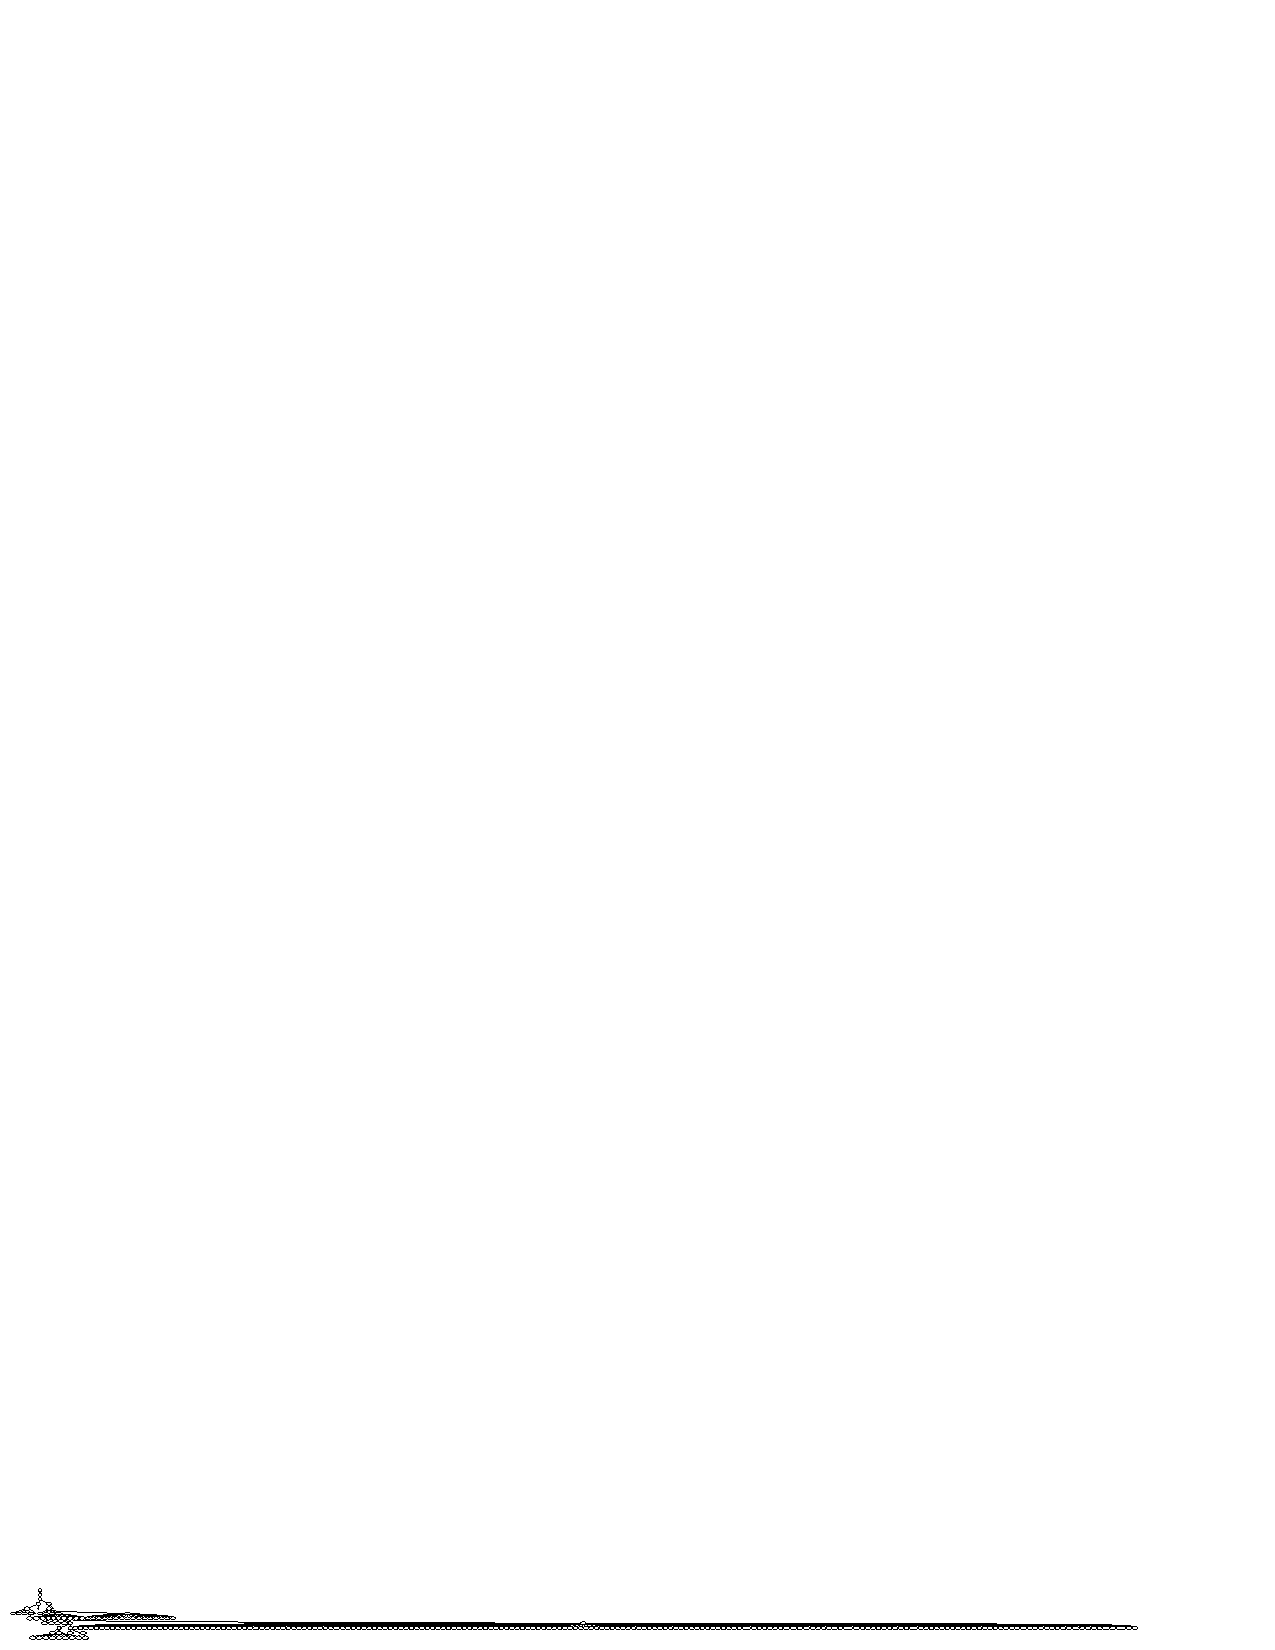
\includegraphics[scale=0.50]{\TopSourceDirectory/docs/Rose/asm_code_samples_gcc}
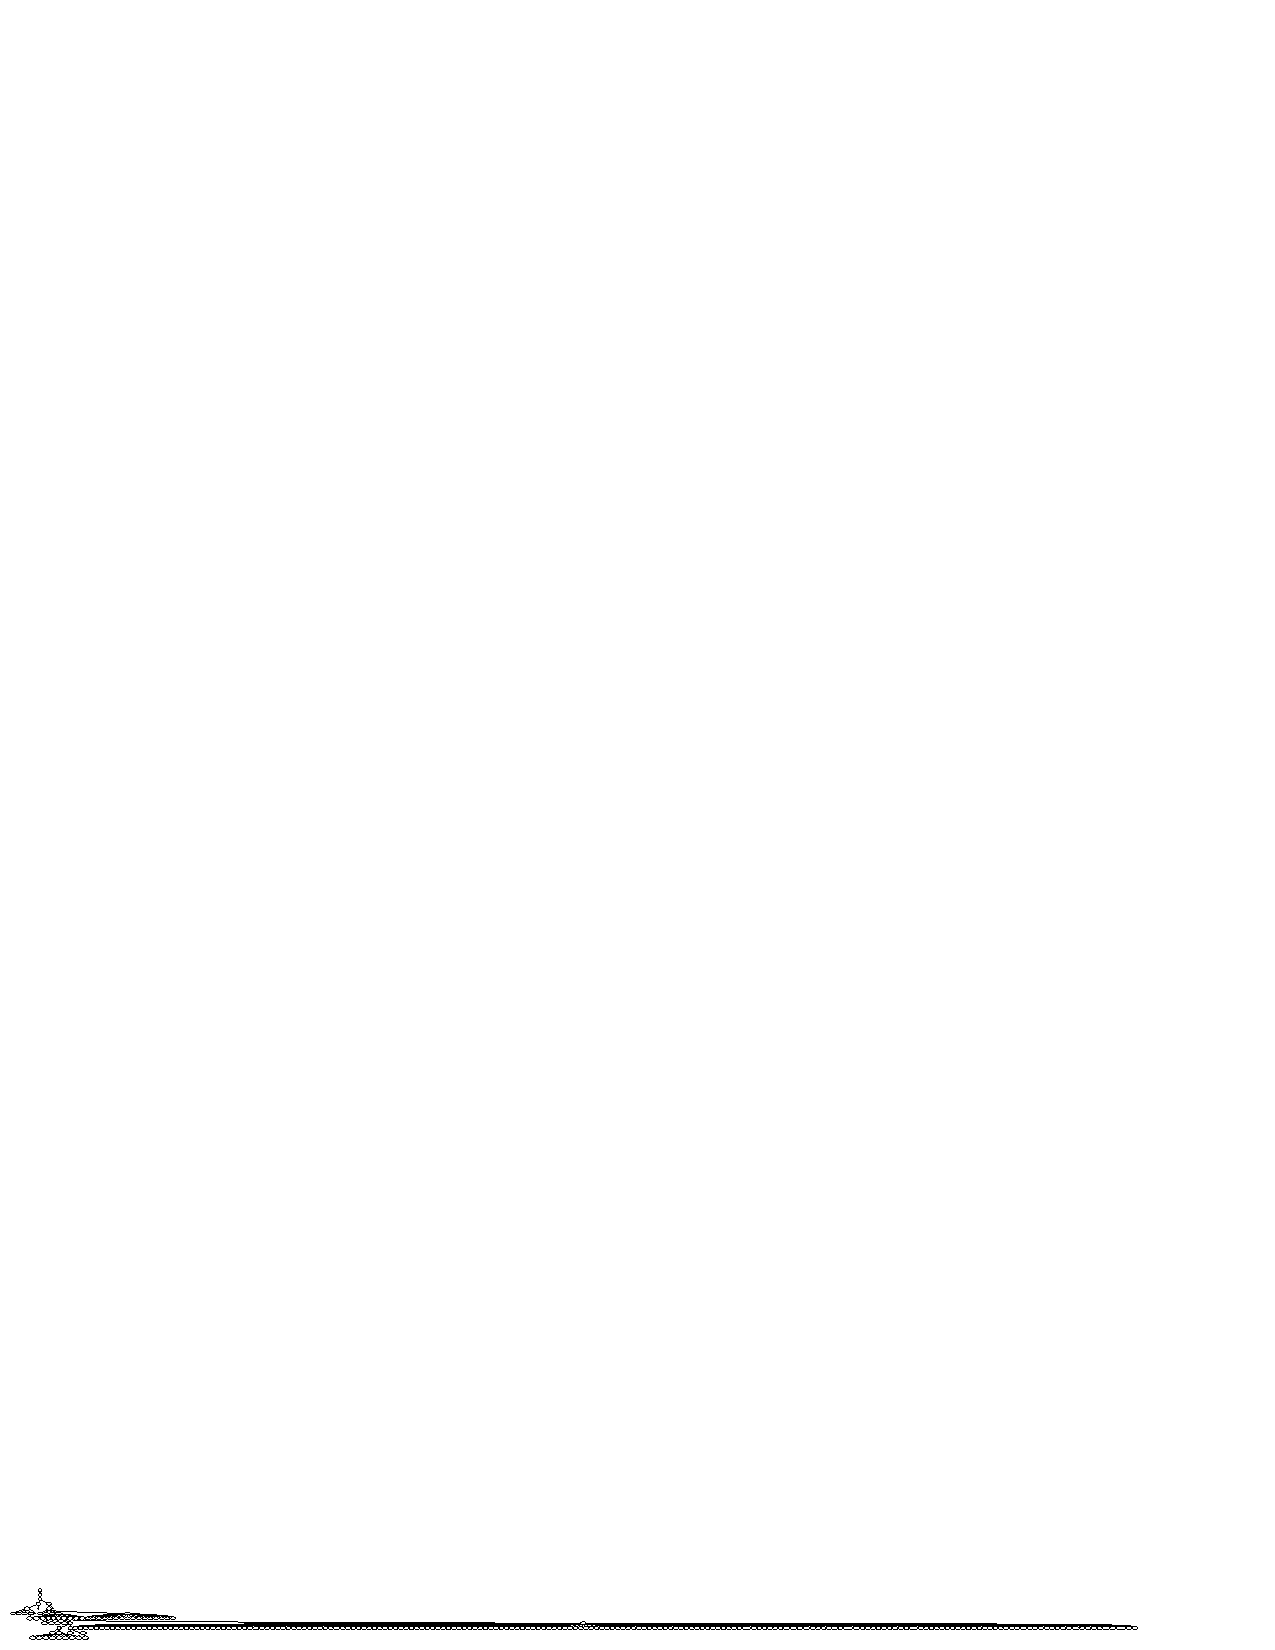
\includegraphics[,viewport=5 1 100 30,scale=2]{\TopSourceDirectory/docs/Rose/asm_code_samples_gcc}
\caption{The AST for a PE (Windows) binary executable (binary file format only), with long
    list of symbols (half of which are clipped on the right side of the image).} 

\label{binaryAnalysis:BinaryExecutableFormatAST_1}
\end{figure}

Figure \ref{binaryAnalysis:BinaryExecutableFormatAST_1} shows the graph of the AST
formed by just the binary file format (sections, symbols, etc.).  This figure shows
the different IR nodes used to represent the binary file format (without the disassembled 
instructions, in this case) and the large list of symbols within the symbol table (the 
long list that is partially truncated on the right edge of the figure).
This graph is quite large and does not fit well on the page, the next figure
\ref{binaryAnalysis:BinaryExecutableFormatAST_2} shows a clipped image with more detail.


\begin{figure}
% \includegraphics[angle=90,scale=0.75,width=5in,height=1in]{\TopSourceDirectory/src/frontend/ExecFormats/BinaryFileFormat}
\includegraphics*[angle=90,viewport=5 1 40 30,scale=18]{\TopSourceDirectory/docs/Rose/asm_code_samples_gcc}
\caption{The CROPPED AST for a PE (Windows) binary executable (binary file format only).} 

\label{binaryAnalysis:BinaryExecutableFormatAST_2}
\end{figure}

Figure \ref{binaryAnalysis:BinaryExecutableFormatAST_2} shows a cropped view of the graph
of the AST formed by just the binary file format (sections, symbols, etc.).  This figure
shows two {\em SgAsmInterpretation} IR nodes; this is a Windows PE binary and all windows
PE binaries contain both a 16-bit MS-DOS header (and some 16-bit code) and a 32-bit Windows
PE header (with sections that have 32-bit code); thus there are two SgAsmInterpretation IR
nodes (one for the 16-bit interpretation of the instructions and one for the 32-bit 
interpretation of the instructions).  Note that ELF format files will have only one
SgAsmInterpretation IR nodes (because there is only a single interpretation possible), but
other file formats can contain many interpretations; formed form a composite of code to
support wide ranges of portability.

*Note: The actually file used is in these figures is: {\tt ROSE/docs/Rose/asm\_code\_samples\_gcc.pdf}.

\subsection{Instruction Disassembly}
% NOTE: This subsection comes almost verbatim from the doxygen documentation in Disassembler.h

ROSE has its own disassembler (for x86, ARM, and PowerPC); a recursive disassembler that is well suited to details of variable
length instruction set handling and data stored in the instruction stream.  All details of the instructions, and the operands
and operator expression trees, etc. are stored in the binary AST as separate IR nodes.  The SgAsmInstruction class and its
architecture-specific subclasses represent individual instructions. The arguments for those instructions are represented by the
SgAsmExpression class and subclasses thereof.
\fixme{We need an example of the AST for a few instructions.}

Disassembly normally happens automatically unless the {\tt -rose:read\_executable\_file\_format\_only} switch is specified.
Alternatively, this Disassembler class can be used to explicitly disassemble parts of a file. The Disassembler class
handles all non-architecture-specific details of disassembly, such as where to search for instructions in the address
space and how instructions are concatenated into basic blocks.  The Disassembler has a pure virtual method,
disassembleOne, that is implemented by architecture-specific subclasses and whose purpose is to disassemble one
instruction.

New architectures can be added to ROSE without modifying any ROSE source code. One does this by subclassing an existing
disassembler, overriding any necessary virtual methods, and registering an instance of this subclass with the
{\tt Disassembler::register\_subclass} method.  If the new subclass can handle multiple architectures then a disassembler is
registered for each of those architectures.

When ROSE needs to disassemble something, it calls {\tt Disassembler::lookup}, which in turn calls the {\tt can\_disassemble}
method for all registered disassemblers.  The first disassembler whose {\tt can\_disassemble} returns true is used for the
disassemby.

If an error occurs during the disassembly of a single instruction, the disassembler will throw an exception. When
disassembling multiple instructions the exceptions are saved in a map, by virtual address, and the map is returned to the
caller along with the instructions that were successfully disassembled.

The main interface to the disassembler is the {\tt disassembleBuffer} method. It searches for instructions based on the
heuristics specified in the {\tt set\_search} method, reading instruction bytes from a supplied buffer.  A MemoryMap object is
supplied in order to specify a mapping from virtual address space to offsets in the supplied buffer. The
{\tt disassembleBuffer} method is used by methods that disassemble whole sections, whole interpretations, or whole files; in
turn, it calls {\tt disassembleBlock} which disassembles sequential instructions until a control flow branch is encountered.

A MemoryMap object can be built that describes the entire virtual address space and how it relates to offsets in the
executable file.  This object, together with the entire contents of the file, can be passed to the {\tt disassembleBuffer}
method in order to disassemble the entire executable in one call.  However, if the executable contains multiple
independent interpretations (like a PE file that contains a Windows executable and a DOS executable) then the best
practice is to disassemble each interpretation individually.  The {\tt disassemble} method is convenient for this.

While the main purpose of the Disassembler class is to disassemble instructions, it also needs to be able to group those
instructions into basic blocks (SgAsmBlock) and functions (SgAsmFunction). It uses an instance of the
Partitioner class to do so.  The user can supply a partitioner to the disassembler or have the disassembler create a
default partitioner on the fly.  The user is also free to call the partitioner directly on the InstructionMap object
returned by most of the disassembler methods.

\subsection{Instruction Partitioning}
% NOTE: This subsection comes almost verbatim from the doxygen documentation in Partitioner.h

While the main purpose of the Disassembler class is to disassemble instructions, it also
needs to be able to group those instructions into basic blocks (SgAsmBlock) and functions
(SgAsmFunction). It uses an instance of the Partitioner class to do so.  The
user can supply a partitioner to the disassembler or have the disassembler create a
default partitioner on the fly.  The user is also free to call the partitioner directly
on the InstructionMap object returned by most of the disassembler methods.

When grouping instructions into basic blocks, the partitioner looks at the instruction
type and known successor addresses. A known successor address is a virtual address where
the processor will disassemble and execute the next instruction. Unconditional branch
instructions typically have a single known successor (the branch target); conditional
branches usually have two successors (the following, or fall-through, address and the
branch target); data processing and testing instructions have one successor (the
following address); and interrupt-causing instructions have no known successors. A branch
to a calculated (non-immediate) address does not qualify as a known successor. The
SgAsmInstruction's terminatesBasicBlock virtual method is used to make this
determination.

Once instructions are assigned to basic blocks, the partitioner assigns the basic blocks
to functions using a variety of heuristics, the set of which is determined by the values
specified in the Partioner's {\tt set\_heuristics} method. These are documented in the
SgAsmFunction class (see the FunctionReason enumeration).  When a function is
created, its {\tt reason} attribute will contain a bit vector describing which heuristics
detected this function.

\subsection{Dwarf Debug Support}
% NOTE:

   ROSE can now read the Dwarf debug information stored into binary executables (ELF only
at this point). This information is represented as Dwarf specific IR nodes in the AST and
thus can be optionally used (when it is available in the binary) as part of any binary 
analysis.  Only a few sections are supported at present: {\em .debug\_info},
{\em .debug\_line}, etc.  The dwarf support in ROSE uses {\em libdwarf} and is enabled in
ROSE using a configuration option: {\tt (configure --with-dwarf={\em<path to libdwarf>}}.
Note that {\em libdwarf} is optional, must be separately installed by the user, and
thus is obviously not distributed within ROSE.  
% The future of the Dwarf support in ROSE is not clear, 
We anticipate the Dwarf information in the AST to be useful for performance tools that
operate on the binary executable when the binary executable has been generated to include 
Dwarf debug information.

\section{Binary Analysis}

   A number of binary analysis passes are provided, most are a part of the Compass
framework for software analysis.  See the {\em Compass User Manual} for more details on
supported binary analysis.

   The ROSE tutorial shows a number of binary analysis passes over both the binary
instructions and the executable file format.

\section{Compass as a Binary Analysis Tool}

   Compass is a tool framework for building software analysis tools using rules (on source
code and alternatively directly on binary executables). Compass
reports violations of the rules in the evaluation of the software.  Compass is a
relatively simple application built on top of ROSE.  Most of the complexity and code 
within Compass is that it includes a large collection to rules, each rule has its
own implementation of an arbitrary test over the source code or the binary.  Rules
(checkers) may be defined over the AST or any other graph built within ROSE to store 
program analysis information. See the Compass manual for more details on supported
binary analysis.  The ability to perform analysis of binary executables using Compass 
makes no assumptions that it is compiled with any specific options or that it contains
debug information, symbols, etc.


\section{Static Binary Rewriting}
   As part of general research on transformations of binaries (separate from analysis)
a number of techniques have been developed to support classes of transformations.
This static rewriting of the binary permits the development of performance tools 
that could support the analysis and rewriting of binaries for support of High 
Performance Computing (HPC). A principal focus is on IBM BGL and Cray XT support 
(DOE Office of Science supercomputers).

\subsection{Generic Section/Segment Modifications}
%===============================================================================================================================
%Generic Section/Segment Modifications
%===============================================================================================================================

\subsubsection{1a. Section/Segment file address shifting (low-level)}

   The low-level movement of an ELF Section or Segment within the file address space is performed with
   SgAsmGenericSection::set\_offset.  It changes the location of the section in the file and updates all relative virtual
   addresses (RVAs) that were primarily associated with the moved section.

   The main problems with this function are that it doesn't take into account the file locations of other sections, the file
   alignment constraints of the moved section, or the memory mapping. Specifically, after calling this function to move {\bf.text}
   one byte later in the file:
\begin{itemize}
   \item {\bf.text} might not satisfy its file alignment constraint.

   \item The end of {\bf.text} might overlap with the following section. The ELF unparser has undefined behavior when two sections
     overlap without storing identical bytes at the overlapping regions.

   \item {\bf.text}, if memory mapped (which it surely is), might not be consistent with the mapping of other adjacent or overlapping
     sections. For instance, {\bf.text} is contained in "ELF Load Segment 2" both in the file address space and in the mapped
     memory space. The offset from ELF Load Segment 2 to {\bf.text} must be identical in both file and memory.

   \item RVAs that point to instructions in {\bf.text} can be associated with the {\bf.text} section or with ELF Load Segment 2,
     depending on how they were parsed. Normally it doesn't matter which since the relationship between file address space and
     memory address space is consistent. But if you change the file addresses without changing memory addresses then the byte
     to which the RVA points could be ambiguous.
\end{itemize}

   Changes to ELF Section or Segment file addresses are reflected in the ELF Section Table and/or ELF Segment Table. If the
   particular SgAsmGenericSection is present in both tables then modifying its file address will result in updates to both
   tables.

   NOTE: Do not modify section offsets and sizes by modifying the section table entries. Changes to these values will be
   overwritten with actual, current section offsets and sizes when the section table is unparsed:
\begin{itemize}
	\item SgAsmElfSectionTableEntry::set\_sh\_offset
	\item SgAsmElfSectionTableEntry::set\_sh\_size
	\item SgAsmElfSectionTableEntry::set\_sh\_addr
\end{itemize}

   NOTE: Do not modify segment offsets and sizes by modifying the segment table entries. Changes to these values will be
   overwritten with actual, current segment offsets and sizes when the segment table is unparsed:
\begin{itemize}
   \item SgAsmElfSegmentTableEntry::set\_offset
   \item SgAsmElfSegmentTableEntry::set\_filesz
   \item SgAsmElfSegmentTableEntry::set\_vaddr
   \item SgAsmElfSegmentTableEntry::set\_memsz
\end{itemize}

\subsubsection{1b. Section/Segment file address shifting (high-level)}
   
   The SgAsmGenericFile::shift\_extend method is the preferred way to make minor offset and/or size adjustments to an ELF
   Section or Segment. It is able to shift a section to a high file and/or memory address and/or extend the segment:
\begin{itemize}
   \item It takes into account all sections in the file, adjusting their offsets and/or sizes accordingly.

   \item Sections to the right of the the section in question (Sq) are shifted upward to make room and prevent overlaps.

   \item Sections overlapping with Sq are extended to contain all of what they previously contained.

   \item The shift amounts are adjusted to satisfy alignment constraints of all affected sections.

   \item Unreferenced areas of the file can optionally be utilized as unused address space.

   \item Adjusting file address spaces also adjusts the memory address spaces in a compatible manner.
\end{itemize}

   NOTE: Do not modify section offsets and sizes by modifying the section table entries. Changes to these values will be
   overwritten with actual, current section offsets and sizes when the section table is unparsed:
\begin{itemize}
	\item SgAsmElfSectionTableEntry::set\_sh\_offset
	\item SgAsmElfSectionTableEntry::set\_sh\_size
	\item SgAsmElfSectionTableEntry::set\_sh\_addr
\end{itemize}

   NOTE: Do not modify segment offsets and sizes by modifying the segment table entries. Changes to these values will be
   overwritten with actual, current segment offsets and sizes when the segment table is unparsed:
\begin{itemize}
   \item SgAsmElfSegmentTableEntry::set\_offset
   \item SgAsmElfSegmentTableEntry::set\_filesz
   \item SgAsmElfSegmentTableEntry::set\_vaddr
   \item SgAsmElfSegmentTableEntry::set\_memsz
\end{itemize}

\subsubsection{2a. Section/Segment resizing (low-level)}

   The size of an ELF Section or Segment can be modified by calling SgAsmGenericSection::set\_size (for file size) and
   set\_mapped\_size (for mapped memory). However, this is a low-level interface that doesn't take into account other sections in
   the same file.  The preferred way to resize a section is with SgAsmGenericFile::shift\_extend.

   NOTE: For many kinds of sections, making the section larger will create an unreferenced area ("internal hole") at the end of
   the section. Other sections will automatically do something with the new address space (e.g., SgAsmElfStringSection will
   add the new address space to its free list).

\subsubsection{2b. Section/Segment resizing (high-level)}

   The preferred way to extend a section is to call SgAsmGenericFile::shift\_extend, which extends sections that contain the
   resized-section and shifts sections that are right (higher address) of the resized-section.  This function also takes into
   account alignment constraints, memory address space, and (optionally) holes in the address space.

\subsection{Modifications to the ELF File Header}
%===============================================================================================================================
%Modifications to the ELF File Header
%===============================================================================================================================

\subsubsection{1. Entry Point RVA}

   The entry RVA stored in the ELF File Header is adjusted whenever the section into which it points is moved in memory. It is
   also possible to adjust this address explicitly by modifying the first (and only) entry in SgAsmGenericHeader::entry\_rvas.

   NOTE: An RVA (rose\_rva\_t) is an offset with respect to the beginning of some section. If the section starting memory address
   changes then the RVA implicitly changes (RVA's are virtual addresses relative to some format-wide base address). Multiple
   sections can be mapped to the same memory (e.g., {\bf.text} and {\bf ELF Load Segment 2} are typically overlap in memory), but
   since an RVA is associated with only one section, modifying the other section(s) has no effect on the RVA even if the RVA
   happens to be inside the other sections as well.

   NOTE: The binding between an RVA and a section can be modified with rose\_rva\_t::set\_section. In fact, the link can be
   completely broken by passing a null section pointer, in which case the RVA is not relative to any section.

\subsubsection{2. File Format Byte order}

   File byte order can be changed by modifying the SgAsmGenericFormat object pointed to by the file header:

      SgAsmGenericHeader *fhdr = ....;
      fhdr->get\_exec\_format()->set\_sex(ORDER\_MSB);

   NOTE: Modifying the byte order affects only those sections that are actually parsed. If the ELF file contains a section
   whose purpose we don't recognize then the original section data is written to the new file.

\fixme{If the byte order is not specified in the ELF header (e\_ident\_data\_encoding other than 1 or 2) then the parser will
   make an educated guess and assign a byte order.  The unparsed file will differ from the original in this case at the sixth
   byte of the file.}

\subsubsection{3. ELF Word Size}

   File word size can be changed between 4 bytes and 8 bytes by modifying the SgAsmGenericFormat object pointed to by the file
   header:

      SgAsmGenericHeader *fhdr = ....;
      fhdr->get\_exec\_format()->set\_word\_size(4);

   When changing word sizes, any fields that have values too large to represent in the new word size will cause the unparser
   to abort.

   NOTE: Modifying the word size affects only those sections that are actually parsed. If the ELF file contains a section whose
   purpose we don't recognize then the original section data is written to the new file.

\fixme{Increasing word size probably requires allocating more space for many of the sections. Vice versa for decreasing the
   word size.}

\subsubsection{4. ELF Header Magic Number}

   An ELF header has a four-byte magic number, usually 0x7f, 'E', 'L', 'F'.  The magic number can be modified by changing the
   string from SgAsmGenericHeader::get\_magic.  It must be exactly four characters in length.

\subsubsection{5. ELF File Purpose (lib, executable, core, etc.)}

   The file purpose should be modified by setting two fields, using

\begin{enumerate}
      \item SgAsmElfFileHeader::set\_p\_e\_type
      \item SgAsmGenericFormat::set\_purpose
\end{enumerate}

   Both members should be set to compatible values. The former is the value from the ELF specification and the latter is a
   constant: PURPOSE\_UNSPECIFIED, PURPOSE\_LIBRARY, PURPOSE\_EXECUTABLE, PURPOSE\_CORE\_DUMP, PURPOSE\_PROC\_SPECIFIC, PURPOSE\_OTHER.

\fixme{set\_p\_e\_type should probably call set\_purpose, but we can't go the other direction because the mapping is N:1.}

\subsubsection{6. ELF Version}

   To change the ELF version assign a new value by calling set\_version on the object returned by
   SgAsmGenericHeader::get\_exec\_format.  This doesn't have any effect on the code generated by the unparser since the parser
   only knows about ELF format 1.
   
\subsubsection{7. ELF Target Architecture}

   Modify the target architecture by calling two functions:

       SgAsmElfHeader::set\_e\_machine -- sets the ELF specific value
       SgAsmGenericHeader::set\_isa   -- sets the generic value

   You should call both with consistent values.

\subsubsection{8. ELF Section or Segment Table location}

   The SgAsmElfFileHeader::set\_e\_shoff and set\_e\_phoff methods have been removed since calling them had no lasting effect
   anyway. Instead, if you want to change one of these values for unparsing, then modify the actual SgAsmGenericSection that
   holds the table (e.g., calling SgAsmGenericFile::shift\_extend).

\subsubsection{9. ELF Section or Segment Table size}

   The number of entries in the section or segment table cannot be modified by calling set\_e\_shnum or set\_e\_phnum on the
   SgAsmElfFileHeader \fixme{Remove these functions.}. Rather, the sizes are obtained by looking at what sections and segments
   are currently defined and writing an entry to the file for each one.

\subsubsection{10. ELF Section Names}

   Elf section names can be modified. Doing so may cause extensive changes to the executable due to reallocation of the section
   holding the string table.

   Do not call SgAsmElfSectionTableEntry::set\_sh\_name since that value will be overwritten based on the actual, current
   location of the name in the associated string table.

\subsubsection{11. ELF Segment Names}

   ELF segment names are often parser-generated based on constants in the ELF Segment Table. However, if the segment
   corresponds to an actual ELF Section defined in the ELF Section Table then the segment and section share the same
   SgAsmGenericSection object and changing the name causes the ELF Section name to change with no effect on the segment table.

\subsubsection{12. ELF Section Name Table}

   The section that holds the section names is identified in the ELF File Header (get\_e\_shstrndx). Although it is possible to
   change this value, doing so will have no effect on the currently-defined sections: they will continue to use the original
   string table for their names.

\subsection{Modifications to ELF String Tables and their Containing Sections}
%===============================================================================================================================
%Modifications to ELF String Tables and their Containing Sections
%===============================================================================================================================

\subsubsection{1. Move/Extend}

   See SgGenericFile::shift\_extend.  When a string table is extended the new address space is added to the table's free list.

\subsubsection{2. New String}

   A new string can be created by calling the SgAsmStoredString allocator and passing a string table (something derived from
   SgAsmGenericStrtab) and the initial string value.  The string is not actually allocated space in the file until the new file
   is unparsed or until someone calls SgAsmStoredString::get\_offset.

\subsubsection{3. Value modification}

   A string can be modified by assigning a new value via SgAsmStoredString::set\_string. Storage is not allocated for the new
   value until the AST is unparsed or someone calls SgAsmStoredString::get\_offset.  The previous value is freed.

\subsubsection{4. Shared strings}

   Three forms of sharing are supported:

\begin{enumerate}
   \item Two objects (section names, symbol names, etc) share the same string and changing one string causes the other to change
      as well. This kind of sharing is not typically encountered in ELF although the underlying string table classes support
      it.

   \item Two objects have independent strings that happen to have the same value and point to the same offset in the string
      table. In this case, changing one string doesn't change the other. This kind of sharing is often encountered in ELF.

   \item Two objects have independent strings and one is an ending substring of another (e.g., "main" and "domain"). Changing one
      string does not affect the other. This kind of sharing is also common in ELF.
\end{enumerate}

\subsubsection{5. String table internal holes}

   If a sequence of bytes in a string table is not referenced by anything known to the parser, then those bytes are marked as
   internal holes and are prevented from moving with respect to the beginning of the string table. Internal holes are not
   placed on the string table free list (because something we didn't parse might be pointing to them).  The internal holes are
   available with SgAsmGenericSection::congeal.

\subsubsection{6. Reallocation of all strings}

   A string table can be repacked by freeing all it's strings and then reallocating.  We can reallocate around the internal
   holes or through the internal holes.

       strtab.free\_all\_strings();   /* free\_all\_strings(true) blows away internal holes */
       strtab.reallocate();

   The ELF allocator will do its best to overlap storage (e.g., "domain" overlaps with "main").

\subsubsection{7. Deletion of a string}

   A string is deleted by changing its value to the empty string.

\subsubsection{8. Stored strings vs. non-stored strings.}

   If a string value has storage space in a file (such as an ELF Section name), then it's an instance of
   SgAsmStoredString. Otherwise the string is either an std::string or SgAsmBasicString. SgAsmBasicString and SgAsmStoredString
   both derive from SgAsmGenericString.  Changing the value of an SgAsmBasicString has no effect on the unparsed file.

\subsection{Modifications ELF Section Table Entries}
%===============================================================================================================================
%Modifications ELF Section Table Entries
%===============================================================================================================================

Every ELF Section defined by the ELF Section Table is parsed as an SgAsmElfSection, which is derived from SgAsmGenericSection.
The SgAsmElfSection::get\_section\_entry returns a pointer to the ELF Section Table Entry (SgAsmElfSectionTableEntry). Some
members of these objects can be modified and some can't.

\subsubsection{1. These functions should not be called since their values are overwritten during the unparse phase:}

\begin{itemize}
   \item SgAsmElfSectionTableEntry::set\_sh\_name   -- see SgAsmGenericSection::set\_name
   \item SgAsmElfSectionTableEntry::set\_sh\_addr   -- see SgAsmGenericFile::shift\_extend
   \item SgAsmElfSectionTableEntry::set\_sh\_offset -- see SgAsmGenericFile::shift\_extend
   \item SgAsmElfSectionTableEntry::set\_sh\_size   -- see SgAsmGenericFile::shift\_extend
   \item SgAsmElfSectionTableEntry::set\_sh\_link   -- don't call (no alternative yet)
\end{itemize}
   
\subsubsection{2. Can modify}

\fixme{What text should go here?}

\begin{itemize}
   \item SgAsmElfSectionTableEntry::set\_sh\_type
   \item SgAsmElfSectionTableEntry::set\_sh\_flags, although the Write and Execute bits are ignored
   \item SgAsmElfSectionTableEntry::set\_sh\_info      \fixme{Is this complete?}
   \item SgAsmElfSectionTableEntry::set\_sh\_addralign \fixme{Is this complete?}
   \item SgAsmElfSectionTableEntry::set\_sh\_entsize   \fixme{Is this complete?}
\end{itemize}


\section{Dynamic Analysis Support}
\label{intel_pin}

   Recent work in ROSE has added support for dynamic analysis and for mixing of dynamic
and static analysis using the Intel Pin framework. This optional support in ROSE
requires a configure option ({\tt --with-IntelPin=$<path$>}.  The {\tt path} in
the configure option is the path to the top level directory of the location of
the Intel Pin distribution.  This support for Intel Pin has only been tested
on a 64bit Linux system using the most recent distribution of Intel Pin (version 2.6).

Note: The dwarf support in ROSE is currently incompatible with the dwarf support in
Intel Pin.  A message in the configuration of ROSE will detect if both support for
Dwarf and Intel Pin are both specified and exit with an error message that they
are incompatible options.


\section{Usage}
     See the ROSE Tutorial for examples.




\chapter{Binary Construction}

ROSE is normally used in such a way that a file (source code or
binary) is parsed to construct an AST, then operations are performed
on the AST, and the modified AST is unparsed to create a new source or
binary file.  However, it is also possible to construct an AST
explicitly without parsing and then use that AST to generate the
output.  The AST construction interface for binary files was designed
so that working files could be created simply, while still providing
methods to control the finer details of the resulting file.

The example in this chapter shows how to construct a statically linked
ELF executable containing a small ``.text'' section that simply causes
the process to exit with a specific non-zero value.

\section{Constructors}

The AST node constructors are designed to construct the tree from the
root down, and thus generally take the parent node as an
argument. Nodes that refer to other nodes as prerequisites also take
those prerequisites as arguments. For instance, an ELF Relocation
Section is a child of the ELF File Header but also needs an ELF Symbol
Table and therefore takes both objects as constructor arguments.

\section{Read-Only Data Members}

When two or more file formats have a similar notion then that notion
is represented in a base class. However, part of the information may
continue to survive in the specialized class. In these situations
modifications to the specilized data will probably be overridden by
the generic values from the base class.  For instance, all formats
have a notion of byte order which is represented in the base class
SgAsmGenericHeader as little- or big-endian (an enumeration
constant). The ELF specification provides an 8-bit unsigned field to
store the byte order and therefore has potentially more than two
possibilities. Any value assigned to the ELF-specific byte order will
likely be overwritten by the generic byte order before the AST is
unparsed.

A similar situation arises with section offsets, sizes, memory
mappings, permissions, etc. The SgAsmGenericSection class represents
ELF Sections, ELF Segments, PE Objects, and other contiguous regions
of a file and has methods for obtaining/setting these values. In
addition, many of the formats have some sort of table that describes
these sections and which also contains similar information (e.g., the
ELF Segment Table, a.k.a., the ELF Program Header Table). As above,
the generic representation of these notions (stored in
SgAsmGenericSection) override the format-specific values (stored in
SgAsmElfSegmentEntry).

ROSETTA doesn't make a distinction between data members that can be
user-modified and data members that should be modified only by the
parser. Therefore it is up to the user to be aware that certain data
members will have their values computed or copied from other locations
in the AST during the unparsing phase.

\section{Constructing the Executable File Container}

All executable files are stored as children of an SgAsmGenericFile
node. The children are file format headers (SgAsmGenericHeader) such
as an ELF File Header (SgAsmElfFileHeader). This design allows a
single executable file to potentially contain more than one executable
and is used by formats like Windows-PE where the file contains a DOS
File Header as well as a PE File Header.

For the purposes of this example the SgAsmGenericFile node will serve
as the root of the AST and therefore we do not need to specify a
parent in the constructor argument list.

\begin{verbatim}
SgAsmGenericFile *ef = new SgAsmGenericFile;
\end{verbatim}

\section{Constructing the ELF File Header}

The ELF File Header is the first thing in the file, always at offset
zero. File headers are always children of an SgAsmGenericFile which is
specified as the constructor argument.

The section constructors (a file header is a kind of section) always
create the new section so it begins at the current end-of-file and
contains at least one byte. This ensures that each section has a
unique starting address, which will be important when file memory is
actually allocated and sections need to be moved around--the allocator
needs to know the relative positions of the sections in order to
correctly relocate them.

If we were parsing an ELF file we would usually use ROSE's frontend()
method. However, one can also parse the file by first constructing the
SgAsmElfFileHeader and then invoking its parse() method, which parses
the ELF File Header and everything that can be reached from that
header.

We use the typical 0x400000 as the virtual address of the main LOAD
segment, which occupies the first part of the file up through the end
of the ``.text'' section (see below). ELF File Headers don't actually
store a base address, so instead of assigning one to the
SgAsmElfFileHeader we'll leave the header's base address at the
default zero and add base\_va explicitly whenever we need to.

\begin{verbatim}
SgAsmElfFileHeader *fhdr = new SgAsmElfFileHeader(ef);
fhdr->get_exec_format()->set_word_size(8);                  /* default is 32-bit; we want 64-bit */
fhdr->set_isa(SgAsmExecutableFileFormat::ISA_X8664_Family); /* instruction set architecture; default is ISA_IA32_386 */
rose_addr_t base_va = 0x400000;                             /* base virtual address */
\end{verbatim}

\section{Constructing the ELF Segment Table}

ELF executable files always have an ELF Segment Table (also called the
ELF Program Header Table), which usually appears immediately after the
ELF File Header. The ELF Segment Table describes contiguous regions of
the file that should be memory mapped by the loader. ELF Segments
don't have names--names are imparted to the segment by virtue of the
segment also being described by the ELF Section Table, which we'll
create later.

Being a contiguous region of the file, an ELF Segment Table
(SgAsmElfSegmentTable) is derived from SgAsmGenericSection. All
non-header sections have a header as a parent, which we supply as an
argument to the constructor. Since all ELF Segments will be children of
the ELF File Header rather than children of the ELF Segment Table, we
could define the ELF Segment Table at the end rather than here. But
defining it now is an easy way to get it located in its usuall
location immediately after the ELF File Header.

\begin{verbatim}
SgAsmElfSegmentTable *segtab = new SgAsmElfSegmentTable(fhdr);
\end{verbatim}

\section{Constructing the .text Section}

ROSE doesn't treat a ``.text'' section as being anything particularly
special--it's just a regular SgAsmElfSection, which derives from
SgAsmGenericSection. However, in this example, we want to make sure
that our ``.text'' section gets initialized with some
instructions. The easiest way to do that is to specialize
SgAsmElfSection and override or augment a few of the virtual
functions.

We need to override two functions. First, the calculate\_sizes()
function should return the size we need to store the
instructions. We'll treat the instructions as an array of entries each
entry being one byte of the instruction stream. In other words, each
``entry'' is one byte in length consisting of one required byte and no
optional bytes.

We need to also override the unparse() method since the base class
will just fill the ``.text'' section with zeros. The
SgAsmGenericSection::write method we use will write the instructions
starting at the first byte of the section.

Finally, we need to augment the reallocate() method. This method is
reponsible for allocating space in the file for the section and
performing any other necessary pre-unparsing actions. We don't need to
allocate space since the base class's method will take care of that in
conjuction with our version of calculate\_sizes(), but we do need to
set a special ELF flag (SHF\_ALLOC) in the ELF Segment Table entry for
this section. There's a few ways to accomplish this. We do it this way
because the ELF Section Table Entry is not created until later and we
want to demonstrate how to keep all .text-related code in close
proximity.

\begin{verbatim}
class TextSection : public SgAsmElfSection {
public:
    TextSection(SgAsmElfFileHeader *fhdr, size_t ins_size, const unsigned char *ins_bytes)
	: SgAsmElfSection(fhdr), ins_size(ins_size), ins_bytes(ins_bytes)
	{}
    virtual rose_addr_t calculate_sizes(size_t *entsize, size_t *required, size_t *optional, size_t *entcount) const {
	if (entsize)  *entsize  = 1;                        /* an "entry" is one byte of instruction */
	if (required) *required = 1;                        /* each "entry" is also stored in one byte of the file */
	if (optional) *optional = 0;                        /* there is no extra data per instruction byte */
	if (entcount) *entcount = ins_size;                 /* number of "entries" is the total instruction bytes */
	return ins_size;                                    /* return value is section size required */
    }
    virtual bool reallocate() {
	bool retval = SgAsmElfSection::reallocate();        /* returns true if size or position of any section changed */
	SgAsmElfSectionTableEntry *ste = get_section_entry();
	ste->set_sh_flags(ste->get_sh_flags() | 0x02); /* set the SHF_ALLOC bit */
	return retval;
    }
    virtual void unparse(std::ostream &f) const {
	write(f, 0, ins_size, ins_bytes);                   /* Write the instructions at offset zero in section */
    }
    size_t ins_size;
    const unsigned char *ins_bytes;
};
\end{verbatim}

The section constructors and reallocators don't worry about alignment
issues--they always allocate from the next available byte. However,
instructions typically need to satisfy some alignment constraints. We
can easily adjust the file offset chosen by the constructor, but we
also need to tell the reallocator about the alignment constraint. Even
if we didn't ever resize the ``.text'' section the reallocator could
be called for some other section in such a way that it needs to move
the ``.text'' section to a new file offset.

For the purpose of this tutorial we want to be very picky about the
location of the ELF Segment Table. We want it to immediately follow
the ELF File Header without any intervening bytes of padding. At the
current time, the ELF File Header has a size of one byte and will
eventually be reallocated. When we reallocate the header the
subsequent sections will need to be shifted to higher file
offsets. When this happens, the allocator shifts them all by the same
amount taking care to satisfy all alignment constraints, which means
that an alignment constraint of byte bytes on the ``.text'' section
will induce a similar alignment on the ELF Segment Table. Since we
don't want that, the best practice is to call reallocate() now, before
we create the ``.text'' section.

\begin{verbatim}
ef->reallocate();                                           /* Give existing sections a chance to allocate file space */
static const unsigned char instructions[] = {0xb8, 0x01, 0x00, 0x00, 0x00, 0xbb, 0x56, 0x00, 0x00, 0x00, 0xcd, 0x80};
SgAsmElfSection *text = new TextSection(fhdr, NELMTS(instructions), instructions);
text->set_purpose(SgAsmGenericSection::SP_PROGRAM);         /* Program-supplied text/data/etc. */
text->set_offset(alignUp(text->get_offset(), 4));           /* Align on an 8-byte boundary */
text->set_file_alignment(4);                                /* Tell reallocator about alignment constraint */
text->set_mapped_alignment(4);                              /* Alignment constraint for memory mapping */
text->set_mapped_rva(base_va+text->get_offset());           /* Mapped address is based on file offset */
text->set_mapped_size(text->get_size());                    /* Mapped size is same as file size */
text->set_mapped_rperm(true);                               /* Readable */
text->set_mapped_wperm(false);                              /* Not writable */
text->set_mapped_xperm(true);                               /* Executable */
\end{verbatim}

At this point the text section doesn't have a name. We want to name it
``.text'' and we want those characters to eventually be stored in the
ELF file in a string table which we'll provide later. In ELF, section
names are represented by the section's entry in the ELF Section Table
as an offset into an ELF String Table for a NUL-terminated ASCII
string. ROSE manages strings using the SgAsmGenericString class, which
has two subclasses: one for strings that aren't stored in the
executable file (SgAsmBasicString) and one for strings that are stored
in the file (SgAsmStoredString). Both are capable of string an
std::string value and querying its byte offset (although
SgAsmBasicString::get\_offset() will always return
SgAsmGenericString::unallocated).  Since we haven't added the
``.text'' section to the ELF Section Table yet the new section has an
SgAsmBasicString name. We can assign a string to the name now and the
string will be allocated in the ELF file when we've provided further
information.

\begin{verbatim}
text->get_name()->set_string(".text");
\end{verbatim}

The ELF File Header needs to know the virtual address at which to
start running the program. In ROSE, virtual addresses can be attached
to a specific section so that if the section is ever moved the address
is automatically updated. Some formats allow more than one entry
address which is why the method is called add\_entry\_rva() rather than
set\_entry\_rva(). ELF, however, only allows one entry address.

\begin{verbatim}
rose_rva_t entry_rva(text->get_mapped_rva(), text);
fhdr->add_entry_rva(entry_rva);
\end{verbatim}

\section{Constructing a LOAD Segment}

ELF Segments define parts of an executable file that should be mapped
into memory by the loader.  A program will typically have a LOAD
segment that begins at the first byte of the file and continues
through the last instruction (in our case, the end of the ``.text''
section) and which is mapped to virtual address 0x400000.

We've already created the ELF Segment Table, so all we need to do now
is create an ELF Segment and add it to the ELF Segment Table. ELF
Segments, like ELF Sections, are represented by SgAsmElfSection. An
SgAsmElfSection is an ELF Section if it has an entry in the ELF
Section Table, and/or it's an ELF Segment if it has an entry in the
ELF Segment Table. The methods get\_section\_entry() and
get\_segment\_entry() retrieve the actual entries in those tables.

Recall that the constructor creates new sections located at the
current end-of-file and containing one byte. Our LOAD segment needs to
have a different offset and size.

\begin{verbatim}
SgAsmElfSection *seg1 = new SgAsmElfSection(fhdr);          /* ELF Segments are represented by SgAsmElfSection */
seg1->get_name()->set_string("LOAD");                       /* Segment names aren't saved (but useful for debugging) */
seg1->set_offset(0);                                        /* Starts at beginning of file */
seg1->set_size(text->get_offset() + text->get_size());      /* Extends to end of .text section */
seg1->set_mapped_rva(base_va);                              /* Typically mapped by loader to this memory address */
seg1->set_mapped_size(seg1->get_size());                    /* Make mapped size match size in the file */
seg1->set_mapped_rperm(true);                               /* Readable */
seg1->set_mapped_wperm(false);                              /* Not writable */
seg1->set_mapped_xperm(true);                               /* Executable */
segtab->add_section(seg1);                                  /* Add definition to ELF Segment Table */
\end{verbatim}

\section{Constructing a PAX Segment}

This documentation shows how to construct a generic ELF Segment,
giving it a particular file offset and size. ELF Segments don't have
names stored in the file, but we can assign a name to the AST node to
aid in debugging--it just won't be written out. When parsing an ELF
file, segment names are generated based on the type stored in the
entry of the ELF Segment Table. For a PAX segment we want this type to
be PT\_PAX\_FLAGS (the default is PT\_LOAD).

\begin{verbatim}
SgAsmElfSection *pax = new SgAsmElfSection(fhdr);
pax->get_name()->set_string("PAX Flags");                   /* Name just for debugging */
pax->set_offset(0);                                         /* Override address to be at zero rather than EOF */
pax->set_size(0);                                           /* Override size to be zero rather than one byte */
segtab->add_section(pax);                                   /* Add definition to ELF Segment Table */
pax->get_segment_entry()->set_type(SgAsmElfSegmentTableEntry::PT_PAX_FLAGS);
\end{verbatim}

\section{Constructing a String Table}

An ELF String Table always corresponds to a single ELF Section of
class SgAsmElfStringSection and thus you'll often see the term ``ELF
String Section'' used interchangeably with ``ELF String Table'' even
though they're two unique but closely tied classes internally.

When the ELF String Section is created a corresponding ELF String
Table is also created under the covers. Since string tables manage
their own memory in reponse to the strings they contain, one should
never adjust the size of the ELF String Section (it's actually fine to
enlarge the section and the new space will become free space in the
string table).

ELF files typically have multiple string tables so that section names
are in a different section than symbol names, etc. In this tutorial
we'll create the section names string table, typically called
``.shstrtab'', but use it for all string storage.

\begin{verbatim}
SgAsmElfStringSection *shstrtab = new SgAsmElfStringSection(fhdr);
shstrtab->get_name()->set_string(".shstrtab");
\end{verbatim}

\section{Constructing an ELF Section Table}

We do this last because we want the ELF Section Table to appear at the
end of the file and this is the easiest way to achieve that. There's
really not much one needs to do to create the ELF Section Table other
than provide the ELF File Header as a parent and supply a string
table.

The string table we created above isn't activated until we assign it
to the ELF Section Table. The first SgAsmElfStringSection added to the
SgAsmElfSectionTable becomes the string table for storing section
names. It is permissible to add other sections to the table before
adding the string table.

\begin{verbatim}
SgAsmElfSectionTable *sectab = new SgAsmElfSectionTable(fhdr);
sectab->add_section(text);                                  /* Add the .text section */
sectab->add_section(shstrtab);                              /* Add the string table to store section names. */
\end{verbatim}

\section{Allocating Space}

Prior to calling unparse(), we need to make sure that all sections
have a chance to allocate space for themselves, and perform any other
operations necessary. It's not always possible to determine sizes at
an earlier time, and most constructors would have declared sizes of
only one byte.

The reallocate() method is defined in the SgAsmGenericFile class since
it operates over the entire collection of sections simultaneously. In
other words, if a section needs to grow then all the sections located
after it in the file need to be shifted to higher file offsets.

\begin{verbatim}
ef->reallocate();
\end{verbatim}

The reallocate() method has a shortcoming (as of 2008-12-19) in that
it might not correctly update memory mappings in the case when the
mapping for a section is inferred from the mapping of a containing
segment. This can happen in our example since the ``.text'' section's
memory mapping is a function of the LOAD Segment mapping. The
work-around is to adjust mappings for these situations and then call
reallocate() one final time. This final reallocate() call won't move
any sections, but should always be the last thing to call before
unparsing() (it gives sections a chance to update data dependencies
which is not possible during unparse() due to its const nature).

\begin{verbatim}
text->set_mapped_rva(seg1->get_mapped_rva()+(text->get_offset()-seg1->get_offset()));
ef->reallocate(); /*won't resize or move things this time since we didn't modify much since the last call to reallocate()*/
\end{verbatim}

\section{Produce a Debugging Dump}

A debugging dump can be made with the following code. This dump will
not be identical to the one produced by parsing and dumping the
resulting file since we never parsed a file (a dump contains some
information that's parser-specific).

\begin{verbatim}
ef->dump(stdout);
SgAsmGenericSectionPtrList all = ef->get_sections(true);
for (size_t i=0; i<all.size(); i++) {
    fprintf(stdout, "Section %zu:\n", i);
    all[i]->dump(stdout, "    ", -1);
}
\end{verbatim}

\section{Produce the Executable File}

The executable file is produced by unparsing the AST.

\begin{verbatim}
std::ofstream f("a.out");
ef->unparse(f);
\end{verbatim}

Note that the resulting file will not be created with execute
permission--that must be added manually.

\chapter{Dwarf Debug Support}

% Copied from the Dwarf wikipedia page.
DWARF is a widely used, standardized debugging data format. DWARF was originally designed
along with ELF, although it is independent of object file formats. The name is a
pun on "ELF" that has no official meaning but "may be an acronym for 'Debug With
Attributed Record Format'".  See Wikipedia for more information about the Dwarf 
debug format.

This chapter presents the support in ROSE for Dwarf 3 debug information; its 
representation in the AST and its use in binary analysis tools.  This work is part of
general work to support as much information as possible about binaries.

In the following sections we use a small example (see figure \ref{Tutorial:dwarfAnalysisExampleSourceCode}) 
that demonstrates various features of Dwarf. The source code of our binary example is:

\commentout{
\begin{figure}[!h]
{\indent
{\mySmallFontSize

% Do this when processing latex to generate non-html (not using latex2html)
\begin{latexonly}
   \lstinputlisting{\TutorialExampleDirectory/dwarfAnalysis.C}
\end{latexonly}

% Do this when processing latex to build html (using latex2html)
\begin{htmlonly}
   \verbatiminput{\TutorialExampleDirectory/dwarfAnalysis.C}
\end{htmlonly}

% end of scope in font size
}
% End of scope in indentation
}
\caption{Example source code (typical for reading in a binary or source file).}
\label{Tutorial:dwarfAnalysisExampleSourceCode}
\end{figure}
}

\begin{figure}[!h]
{\indent
{\mySmallFontSize

% Do this when processing latex to generate non-html (not using latex2html)
\begin{latexonly}
   \lstinputlisting{\TutorialExampleDirectory/inputCode_dwarfAnalysis.C}
\end{latexonly}

% Do this when processing latex to build html (using latex2html)
\begin{htmlonly}
   \verbatiminput{\TutorialExampleDirectory/inputCode_dwarfAnalysis.C}
\end{htmlonly}

% end of scope in font size
}
% End of scope in indentation
}
\caption{Example source code used to generate Dwarf AST for analysis.}
\label{Tutorial:dwarfAnalysisExampleSourceCode}
\end{figure}


Much larger binaries can be analyzed, but such larger binary executables are more
difficult to present (in this tutorial).


\section{ROSE AST of Dwarf IR nodes}

   ROSE tools process the binary into an AST that is used to represent all the
information in the binary executable.  Figure \ref{Tutorial:Dwarf_AST_example}
shows the subset of that AST (which includes the rest of the binary file format
and the disassembled instructions) that is specific to Dwarf.  A command line option
({\em -rose:visualize\_dwarf\_only}) is used to restrict the generated dot file 
visualization to just the Dwarf information. This option is used in combination with 
{\em -rose:read\_executable\_file\_format\_only} to process only the binary file format
(thus skipping the instruction disassembly).

\begin{figure}[h]
{\indent
{\mySmallFontSize

% Do this when processing latex to generate non-html (not using latex2html)
\begin{latexonly}
%  \includegraphics[scale=0.9]{\TutorialExampleBuildDirectory/inputCode_dwarfAnalysis}
   \includegraphics[viewport=5 1 50 500,scale=0.9]{\TutorialExampleBuildDirectory/inputCode_dwarfAnalysis}
\end{latexonly}

% Do this when processing latex to build html (using latex2html)
\begin{htmlonly}
   \includegraphics{\TutorialExampleBuildDirectory/inputCode_dwarfAnalysis}
\end{htmlonly}

% end of scope in font size
}
% End of scope in indentation
}
\caption{Dwarf AST (subset of ROSE binary AST).}
\label{Tutorial:Dwarf_AST_example}
\end{figure}



\section{Source Position to Instruction Address Mapping}

   One of the valuable parts of Dwarf is the mapping between the 
source lines and the instruction addresses at a statement level
(provided in the {\em .debug\_line} section).
Even though Dwarf does not represent all statements in the source
code, the mapping is significantly finer granularity than that
provided at only the function level by the symbol table (which
identifies the functions by instruction address, but not the 
source file line numbers; the later requires source code analysis).

The example code in \ref{Tutorial:dwarfInstructionAddressToSourceLineExampleSourceCode}
shows the mapping between the source code lines and the instruction addresses.

\fixme{This need to be improved to correctly return sets of lines and sets of addresses in
       what might be a second interface.}

\begin{figure}[!h]
{\indent
{\mySmallFontSize

% Do this when processing latex to generate non-html (not using latex2html)
\begin{latexonly}
   \lstinputlisting{\TutorialExampleDirectory/dwarfInstructionAddressToSourceLineAnalysis.C}
\end{latexonly}

% Do this when processing latex to build html (using latex2html)
\begin{htmlonly}
   \verbatiminput{\TutorialExampleDirectory/dwarfInstructionAddressToSourceLineAnalysis.C}
\end{htmlonly}

% end of scope in font size
}
% End of scope in indentation
}
\caption{Example source code (typical for reading in a binary or source file).}
\label{Tutorial:dwarfInstructionAddressToSourceLineExampleSourceCode}
\end{figure}

Output from the compilation of this test code and running it with the example input
results in the output shown in figure \ref{Tutorial:dwarfInstructionAddressToSourceLineExampleOutput}.
This output shows the binary executables instruction address range (binary compiled on
Linux x86 system), the range of lines of source code used by the binary executable,
the mapping of a source code range of line numbers to the instruction addresses,
and the mapping of a range of instruction addresses to the source code line numbers.

%\fixme{Need to handle case of were each query can return a set of line or set of
%       addresses.  This may be a different interface for simplicty.}

\begin{figure}[!h]
{\indent
{\mySmallFontSize

% Do this when processing latex to generate non-html (not using latex2html)
\begin{latexonly}
   \lstinputlisting{\TutorialExampleBuildDirectory/inputCode_dwarfAnalysis.out}
\end{latexonly}

% Do this when processing latex to build html (using latex2html)
\begin{htmlonly}
   \verbatiminput{\TutorialExampleBuildDirectory/inputCode_dwarfAnalysis.out}
\end{htmlonly}

% end of scope in font size
}
% End of scope in indentation
}
\caption{Example source code (typical for reading in a binary or source file).}
\label{Tutorial:dwarfInstructionAddressToSourceLineExampleOutput}
\end{figure}








%-----------------------------------------------------------
%          Interacting with Other Tools
%-----------------------------------------------------------
\part[Interacting with Other Tools]{ Interacting with Other Tools \\
\vspace{1.0in}
\normalsize{How to build interoperable tools using ROSE.}
}
\chapter{Abstract Handles to Language Constructs}
\label{chap:handles}
This chapter describes a reference design and its corresponding implementation for
supporting abstract handles to language constructs in source code and optimization
phases. It can be used to facilitate the interoperability between compilers and tools.
We define an abstract handle as a representation for a unique language construct in a
specific program.  Interoperability between tools is achieved by writing out the abstract handles as
strings and reading them within other tools to build the equivalent abstract handle.
\footnote{Abstract Handles are not appropriate for program analysis
since they are not intended to be used to capture the full structure of a program. Instead, 
Abstract Handles represent references to language constructs in a program, capturing only
a program's local structure; intended to support interoperability between source based
tools (including compilers).  We don't advise the use of abstract handles in an
aggressive way to construct an alternative intermediate representation (IR) for a full
program.}

The idea is to define identifiers for unique statements, loops, functions, 
and other language constructs in source code. Given the diverse user requirements, an
ideal specification should include multiple forms to specify a language construct.

Currently, we are interested in the following forms for specifying language constructs:
\begin{itemize}
   \item Source file position information including path, filename, line and column number etc. 
      GNU standard source position from 
      \url{http://www.gnu.org/prep/standards/html\_node/Errors.html} presents
      some examples.  
   \item Global or local numbering of specified language construct in source file
      (e.g. 2nd "do" loop in a global scope).  The file is itself specified using an
       abstract handle (typically generated from the file name). 
   \item Global or local names of constructs. Some language constructs, such
      as files, function definitions and namespace, have names which can be
      used as their handle within a context.
   \item Language-specific label mechanisms. These include named constructs in Fortran,
      numbered labels in Fortran, and statement labels in C and C++, etc. 
\end{itemize}
In addition to human-readable forms, compilers and tools can generate
internal IDs for language constructs. It is up to compiler/tool developers
to provide a way to convert their internal representations into human-readable formats. 

% We define an abstract handle as a unique representation for a language construct. It can
Abstract Handles can
have any of the human-readable or machine-generated forms. A handle can be used alone or
combined with other handles to specify a language construct. A handle can also be
converted from one form to another (e.g. from a compiler specific form to an human
readable form relative to the source position; filename, line number, etc.).
Abstract handles can have different lifetimes depending on their use and implementation. 
An abstract handle might be required to be persistent if it is used to reference a
language construct that would be optimized over multiple executions of one or more
different tools. Where as an abstract-handle might be internally generated only for
purposes of optimizations used in a single execution (e.g. optimization within a compiler).

\section{Use Case}
   A typical use can for Abstract Handles might be for a performance tool to 
identify a collection of loops in functions that are computationally intensive
and to construct Abstract Handles that refer to this specific loops.  Then
pass the Abstract Handles to a second tool that might analyze the source code
and/or the binary executable to evaluate if the computational costs are reasonable 
or if optimizations might be possible.  The specific goal of the Abstract Handles
is to support these sorts of uses within autotuning using diverse tools used
and/or developed as part of autotuning research within the DOE SciDAC PERI project.

\section{Syntax}
%  A possible specification of language handles can have the following syntax:
   A possible grammar for abstract handles could be:

\begin{verbatim}
/* a handle is a single handle item or a link of them separated by ::, or
other delimiters */
handle ::= handle_item | handle '::' handle_item

/* Each handle item consists of construct_type and a specifier. 
Or it can be a compiler generated id of any forms. */

handle_item ::= construct_type specifier | compiler_generated_handle

/* 
Construct types are implementation dependent.
An implementation can support a subset of legal constructs or all of them.
We define a minimum set of common construct type names here and 
will grow this list as needed.
*/
construct_type ::= Project|SourceFile|FunctionDeclaration|ForStatement|...

/* A specifier is used to locate a particular construct
  e.g: <name, "foo">
*/

specifier::= '<' specifier_type ',' specifier_value '>'                

/* tokens for specifier types could be name, position,numbering, label, etc. 
specifier type is necessary to avoid ambiguity for specifier values, 
because a same value could be interpreted in different specifier types otherwise
*/

specifier_type::= name | position | numbering | label 

/* Possible values for a specifier */

specifier_value::= string_lit|int_lit|position_value| label_value

/*A label could be either integer or string */
label_value::= int_lit | string_lit

/* Start and end source line and column information 
e.g.: 13.5-55.4,  13,  13.5 , 13.5-55 */
position_value:: = line_number[ '.' column_number][ '-' line_number[ '.' column_number]]

/* Integer value: one or more digits */
int_lit ::= [0-9]+

/* String value: start with a letter, followed by zero or more letters or digits */
string_lit ::= [a-z][a-z0-9]*

\end{verbatim}

\section{Examples}
We give some examples of language handles using the syntax mentioned above. 
Canonical AST's node type names are used as the construct type names. 
Other implementations can use their own construct type names.

\begin{itemize}
\item A file handle consisting of only one handle item: 
\begin{verbatim}
SourceFile<name,"/home/PERI/test111.f">
\end{verbatim}

\item A function handle using a named handle item, combined with a parent handle using a name also: 

\begin{verbatim}
SourceFile<name,"/home/PERI/test111.f">::FunctionDeclaration<name,"foo">
\end{verbatim}

\item A function handle using source position(A function starting at line 12, column 1 till line 30, column 1 within a file): 

\begin{verbatim}
SourceFile<name,"/home/PERI/test111.f">::FunctionDeclaration<position,"12.1-30.1">

\end{verbatim}
\item A function handle using numbering(The first function definition in a file): 
\begin{verbatim}
SourceFile<name,/home/PERI/test111.f">::FunctionDeclaration<numbering,1>
\end{verbatim}
\item A return statement using source position (A return statement at line 100):
\begin{verbatim}
SourceFile<name,/home/PERI/test222.c>::ReturnStatement<position,"100">

\end{verbatim}
\item A loop using numbering information (The second loop in function
main()): 
\begin{verbatim}
SourceFile<name,"/home/PERI/test222.c">::FunctionDeclaration<name,"main">::
ForStatement<numbering,2>
\end{verbatim}
\item A nested loop using numbering information (The first loop inside the second loop in function
main()): 
\begin{verbatim}
SourceFile<name,"/home/PERI/test222.c">::FunctionDeclaration<name,"main">::
ForStatement<numbering,2>::ForStatement<numbering,1>
\end{verbatim}

\end{itemize}

\section{Reference Implementation}
Abstract Handles are fundamentally compiler and tool independent, however to
clarify the concepts, provide meaningful examples, a working reference 
implementation we have provided a reference implementation in ROSE.
% Within ROSE we provide a reference implementation of the abstract handle concept. 
The source files are located in \textit{src/midend/abstractHandle} in the ROSE distribution.
A generic interface (abstract\_handle.h and abstract\_handle.cpp) provides
data structures and operations for manipulating abstract handles using source file
positions, numbering, or names. Any compilers and tools can have their own implementations
using the same interface.

\subsection{Connecting to ROSE}
A ROSE adapter (roseAdapter.h and roseAdapter.cpp) using the interface is
provided as a concrete implementation for the maximum capability of the
implementation (within a source-to-source compiler).
Figure~\ref{Tutorial:abstractHandle1} shows the code (using ROSE) to generate abstract
handles for loops in an input source file (as in
Figure~\ref{Tutorial:abstractHandle1input}). 
Abstract handle constructors generate handles from abstract nodes, which are implemented
using ROSE AST nodes. Source position is used by default to generate a handle item. 
Names or numbering are used instead when source position information is not available. 
The Constructor can also be used to generate a handle item using a specified handle type
(numbering handles in the example). Figure~\ref{Tutorial:abstractHandle1out} is the output
showing the generated handles for the loops.

%---------------------example 1. ----------------------
\begin{figure}[!h]
{\indent
{\mySmallFontSize
% Do this when processing latex to generate non-html (not using latex2html)
\begin{latexonly}
  \lstinputlisting{\TutorialExampleDirectory/abstractHandle1.cpp}
\end{latexonly}

% Do this when processing latex to build html (using latex2html)
\begin{htmlonly}
   \verbatiminput{\TutorialExampleDirectory/abstractHandle1.cpp}
\end{htmlonly}

% end of scope in font size
}
% End of scope in indentation
}
\caption{Example 1: Generated handles for loops: using constructors with or without a specified handle type.}
\label{Tutorial:abstractHandle1}
\end{figure}
%------------------ input------------------------------
\begin{figure}[!h]
{\indent
{\mySmallFontSize
% Do this when processing latex to generate non-html (not using latex2html)
\begin{latexonly}
  \lstinputlisting{\TutorialExampleDirectory/inputCode_AbstractHandle1.cpp}
\end{latexonly}

% Do this when processing latex to build html (using latex2html)
\begin{htmlonly}
   \verbatiminput{\TutorialExampleDirectory/inputCode_AbstractHandle1.cpp}
\end{htmlonly}

% end of scope in font size
}
% End of scope in indentation
}
\caption{Example 1: Example source code with some loops, used as input.}
\label{Tutorial:abstractHandle1input}
\end{figure}


%---------------------example 1's output ----------------------
\begin{figure}[!h]
{\indent
{\mySmallFontSize
% Do this when processing latex to generate non-html (not using latex2html)
\begin{latexonly}
  \lstinputlisting{\TutorialExampleBuildDirectory/abstractHandle1.outx}
\end{latexonly}

% Do this when processing latex to build html (using latex2html)
\begin{htmlonly}
   \verbatiminput{\TutorialExampleBuildDirectory/abstractHandle1.outx}
\end{htmlonly}

% end of scope in font size
}
% End of scope in indentation
}
\caption{Example 1: Abstract handles generated for loops.}
\label{Tutorial:abstractHandle1out}
\end{figure}

\clearpage
A second example (shown in Figure~\ref{Tutorial:abstractHandle2})
demonstrates how to create handles using user-specified strings
representing handle items for language constructs within a source file
(shown in Figure~\ref{Tutorial:abstractHandle2input}). 
This is particularly useful to grab internal language constructs from handles provided by external software tools. 
The output of the example is given in Figure~\ref{Tutorial:abstractHandle2out}.

%---------------------example 2. ----------------------
\begin{figure}[!h]
{\indent
{\mySmallFontSize
% Do this when processing latex to generate non-html (not using latex2html)
\begin{latexonly}
  \lstinputlisting{\TutorialExampleDirectory/abstractHandle2.cpp}
\end{latexonly}

% Do this when processing latex to build html (using latex2html)
\begin{htmlonly}
   \verbatiminput{\TutorialExampleDirectory/abstractHandle2.cpp}
\end{htmlonly}

% end of scope in font size
}
% End of scope in indentation
}
\caption{Example 2: Generated handles from strings representing handle items.}
\label{Tutorial:abstractHandle2}
\end{figure}

%------------------ input------------------------------
\begin{figure}[!h]
{\indent
{\mySmallFontSize
% Do this when processing latex to generate non-html (not using latex2html)
\begin{latexonly}
  \lstinputlisting{\TutorialExampleDirectory/inputCode_AbstractHandle2.cpp}
\end{latexonly}

% Do this when processing latex to build html (using latex2html)
\begin{htmlonly}
   \verbatiminput{\TutorialExampleDirectory/inputCode_AbstractHandle2.cpp}
\end{htmlonly}

% end of scope in font size
}
% End of scope in indentation
}
\caption{Example 2: Source code with some language constructs.}
\label{Tutorial:abstractHandle2input}
\end{figure}


%---------------------example 2's output ----------------------
\begin{figure}[!h]
{\indent
{\mySmallFontSize
% Do this when processing latex to generate non-html (not using latex2html)
\begin{latexonly}
  \lstinputlisting{\TutorialExampleBuildDirectory/abstractHandle2.outx}
\end{latexonly}

% Do this when processing latex to build html (using latex2html)
\begin{htmlonly}
   \verbatiminput{\TutorialExampleBuildDirectory/abstractHandle2.outx}
\end{htmlonly}

% end of scope in font size
}
% End of scope in indentation
}
\caption{Example 2: Handles generated from string and their language constructs.}
\label{Tutorial:abstractHandle2out}
\end{figure}

\clearpage
\subsection{Connecting to External Tools}
   A third example is provided to demonstrate how to use the abstract interface
with any other tools, which may have less features in terms of supported language
constructs and their correlations compared to a compiler. 
Assume a tool operating on some simple for-loops within an arbitrary source file (the
input file is not shown in this example). Such a tool might
have an internal data structure representing loops; such as that in given in 
Figure~\ref{Tutorial:myloop}.  We will show how the tool specific data structure
for loops can be used to generate abstract handles and output as strings that can
be used by other tools which use abstract handles (which would generate the
abstract handles by reading the strings).
\begin{figure}[!h]
{\indent
{\mySmallFontSize
% Do this when processing latex to generate non-html (not using latex2html)
\begin{latexonly}
  \lstinputlisting{\TutorialExampleDirectory/../src/midend/abstractHandle/myloop.h}
\end{latexonly}

% Do this when processing latex to build html (using latex2html)
\begin{htmlonly}
   \verbatiminput{\TutorialExampleDirectory/../src/midend/abstractHandle/myloop.h}
\end{htmlonly}

% end of scope in font size
}
% End of scope in indentation
}
\caption{Example 3: A simple data structure used to represent a loop in an arbitrary tool.}
\label{Tutorial:myloop}
\end{figure}

An adapter (loopAdapter.h and loopAdapter.cpp) using the proposed abstract
handle interface is given in \textit{src/midend/abstractHandle}.
It provides a concrete implementation for the interface for the simple loops and adds a
node to support file nodes (Compared to a full-featured IR for a compiler, the
file node is an additional detail for tools without data structures to support files).
The test program is given in Figure ~\ref{Tutorial:testMyLoop}.
Again, it creates a top level file handle first. Then a loop handle
({\em loop\_handle1}) is created within the file handle using its relative numbering information. 
The {\em loop\_handle2} is created from from its string format using file position
information (using GNU standard file position syntax). The {\em loop\_handle3} uses its
relative numbering information within {\em loop\_handle1}.

\begin{figure}[!h]
{\indent
{\mySmallFontSize
% Do this when processing latex to generate non-html (not using latex2html)
\begin{latexonly}
  \lstinputlisting{\TutorialExampleDirectory/../src/midend/abstractHandle/testMyLoop.cpp}
\end{latexonly}

% Do this when processing latex to build html (using latex2html)
\begin{htmlonly}
   \verbatiminput{\TutorialExampleDirectory/../src/midend/abstractHandle/testMyLoop.cpp}
\end{htmlonly}

% end of scope in font size
}
% End of scope in indentation
}
\caption{Example 3: A test program for simple loops' abstract handles.}
\label{Tutorial:testMyLoop}
\end{figure}


The output of the program is shown in Figure~\ref{Tutorial:testMyLoopOutput}.  It
demonstrates the generated strings to represent the abstract handles in the 
arbitrary code operated upon by the tool.  Interoperability is achieved by 
another tool reading in the generated string representation to generate an
abstract handle to the same source code language construct.
%\begin{verbatim}
\begin{figure}[!h]
{\indent
{\mySmallFontSize
\begin{latexonly}
\begin{lstlisting} 
bash-3.00: ./testMyLoop
Created a file handle:
SourceFile<name,file1.c>
Created a loop handle:
SourceFile<name,file1.c>::ForStatement<numbering,1>
Created a loop handle:
SourceFile<name,file1.c>::ForStatement<position,12>
Created a loop handle:
SourceFile<name,file1.c>::ForStatement<numbering,1>::ForStatement<numbering,1>
\end{lstlisting}
\end{latexonly}
% end of scope in font size
}
% End of scope in indentation
}
\caption{Example 3: Output of the test program for simple loops' abstract handles (as strings).}
\label{Tutorial:testMyLoopOutput}
\end{figure}

\clearpage
\section{Summary}

   Abstract handles are low level mechanisms to support multiple tools
to exchange references to source code.  Several examples are used to
present the different features of abstract handles.  Importantly, the 
specification of abstract handles is tool independent.  A reference
implementation is provided and is publically available within the
ROSE compiler framework.  We encourage debate on the pros and cons
of this concept to support interoperability of tools which must
pass references to source code between them.  This work is expected
to a small piece of the infrastructure to suport autotuning research.

%\end{verbatim}


%==========================================================================
\chapter{ROSE-HPCToolKit Interface}
\label{chap:rosehpct}
ROSE-HPCToolKit is designed to read in performance data generated
by HPCToolkit (and recently GNU gprof) and annotate ROSE AST with performance
metrics.
It is included in the ROSE distribution and 
enabled by default if  an existing installation of the Gnome XML library, libxml2
(\url{http://xmlsoft.org}) can be detected by ROSE's configure script.
Or it can be enabled explicitly by specifying the \texttt{--enable-rosehpct} option
when running configure.
% and be sure that you have an existing installation of the Gnome XML library, libxml2 (\url{http://xmlsoft.org}).

The HPCToolkit (\url{http://www.hipersoft.rice.edu/hpctoolkit}) is a
set of tools for analyzing the dynamic performance behavior of
applications. It includes a tool that instruments a program's binary,
in order to observe CPU hardware counters during execution; additional
post-processing tools attribute the observed data to statements in the
original source code. HPCToolkit stores this data and the source
attributions in XML files. In this chapter, we give an overview of
simple interfaces in ROSE that can read this data and attach it to the
AST.

GNU gprof is a basic but easy to use profiling tool.
It produces an execution profile of applications. 
gprof's output is a flat profile for each function by default, which is not
very interesting to us.  
We use a line-by-line output with full file path information generated by using
option {\tt -l -L} with gprof.

\input{\TutorialExampleBuildDirectory/roseHPCT/is-static}

%==========================================================================
\section{An HPCToolkit Example Run}
\label{chap:rosehpct:run}

%--------------------------------------------------------------------------
\begin{figure}[!h]
{\indent
{\mySmallFontSize
% Do this when processing latex to generate non-html (not using latex2html)
\begin{latexonly}
   \lstinputlisting[language=C,numbers=left,stepnumber=5]{\TutorialExampleBuildDirectory/roseHPCT/profiled.c.aa}
\end{latexonly}

% Do this when processing latex to build html (using latex2html)
\begin{htmlonly}
   \verbatiminput{\TutorialExampleBuildDirectory/roseHPCT/profiled.c.aa}
\end{htmlonly}

% end of scope in font size
}
% End of scope in indentation
}
\caption{profiled.c (part 1 of 2): Sample input program, profiled using the HPCToolkit.}
\label{Tutorial:roseHPCT:profiled:aa}
\end{figure}
%--------------------------------------------------------------------------

%--------------------------------------------------------------------------
\begin{figure}[!h]
{\indent
{\mySmallFontSize
% Do this when processing latex to generate non-html (not using latex2html)
\begin{latexonly}
   \lstinputlisting[language=C,numbers=left,stepnumber=5,firstnumber=66]{\TutorialExampleBuildDirectory/roseHPCT/profiled.c.ab}
\end{latexonly}

% Do this when processing latex to build html (using latex2html)
\begin{htmlonly}
   \verbatiminput{\TutorialExampleBuildDirectory/roseHPCT/profiled.c.ab}
\end{htmlonly}

% end of scope in font size
}
% End of scope in indentation
}
\caption{profiled.c (part 2 of 2): Sample input program, profiled using the HPCToolkit.}
\label{Tutorial:roseHPCT:profiled:ab}
\end{figure}
%--------------------------------------------------------------------------

Consider the sample source program shown in
Figures~\ref{Tutorial:roseHPCT:profiled:aa}--\ref{Tutorial:roseHPCT:profiled:ab}.
This program takes an integer $n$ on the command line, and has a
number of loops whose flop and memory-operation complexity are either
$\Theta(n)$ or $\Theta(n^2)$. For this example, we would expect the
loop nest at line 56, which has $O(n^2)$ cost, to be the most
expensive loop in the program for large $n$.

%--------------------------------------------------------------------------
\begin{figure}[!h]
{\indent
{\mySmallFontSize
% Do this when processing latex to generate non-html (not using latex2html)
\begin{latexonly}
   \lstinputlisting[language=XML,numbers=left,stepnumber=5]{\TutorialExampleBuildDirectory/roseHPCT/PAPI_TOT_CYC.xml.aa}
\end{latexonly}

% Do this when processing latex to build html (using latex2html)
\begin{htmlonly}
   \verbatiminput{\TutorialExampleBuildDirectory/roseHPCT/PAPI_TOT_CYC.xml.aa}
\end{htmlonly}

% end of scope in font size
}
% End of scope in indentation
}
\caption{XML schema for HPCToolkit data files: This schema, prepended
to each of the HPCToolkit-generated XML files, describes the format of
the profiling data. This particular schema was generated by HPCToolkit
1.0.4.}
\label{Tutorial:roseHPCT:xml:schema}
\end{figure}
%--------------------------------------------------------------------------

%--------------------------------------------------------------------------
\begin{figure}[!h]
{\indent
{\mySmallFontSize
% Do this when processing latex to generate non-html (not using latex2html)
\begin{latexonly}
   \lstinputlisting[language=XML,numbers=left,stepnumber=5,firstnumber=62]{\TutorialExampleBuildDirectory/roseHPCT/PAPI_TOT_CYC.xml.ab}
\end{latexonly}

% Do this when processing latex to build html (using latex2html)
\begin{htmlonly}
   \verbatiminput{\TutorialExampleBuildDirectory/roseHPCT/PAPI_TOT_CYC.xml.ab}
\end{htmlonly}

% end of scope in font size
}
% End of scope in indentation
}
\caption{PAPI\_TOT\_CYC.xml: Sample cycle counts observed during
profiling, generated from running the HPCToolkit on profiled.c
(Figures~\ref{Tutorial:roseHPCT:profiled:aa}--\ref{Tutorial:roseHPCT:profiled:ab}.)
These lines would appear after the schema shown in
Figure~\ref{Tutorial:roseHPCT:xml:schema}.}
\label{Tutorial:roseHPCT:xml:cycles}
\end{figure}
%--------------------------------------------------------------------------

%--------------------------------------------------------------------------
\begin{figure}[!h]
{\indent
{\mySmallFontSize
% Do this when processing latex to generate non-html (not using latex2html)
\begin{latexonly}
   \lstinputlisting[language=XML,numbers=left,stepnumber=5,firstnumber=62]{\TutorialExampleBuildDirectory/roseHPCT/PAPI_FP_OPS.xml.ab}
\end{latexonly}

% Do this when processing latex to build html (using latex2html)
\begin{htmlonly}
   \verbatiminput{\TutorialExampleBuildDirectory/roseHPCT/PAPI_FP_OPS.xml.ab}
\end{htmlonly}

% end of scope in font size
}
% End of scope in indentation
}
\caption{PAPI\_FP\_OPS.xml: Sample flop counts observed during
profiling, generated from running the HPCToolkit on profiled.c
(Figures~\ref{Tutorial:roseHPCT:profiled:aa}--\ref{Tutorial:roseHPCT:profiled:ab}.)
These lines would appear after the schema shown in
Figure~\ref{Tutorial:roseHPCT:xml:schema}.}
\label{Tutorial:roseHPCT:xml:flops}
\end{figure}
%--------------------------------------------------------------------------

Suppose we use the HPCToolkit to profile this program, collecting
cycle counts and floating-point instructions.\footnote{In this
example, HPCToolkit uses the PAPI to read CPU counters
(\url{http://icl.cs.utk.edu/papi}).} HPCToolkit will generate one XML
file for each metric.

A schema specifying the format of these XML files appears in
Figure~\ref{Tutorial:roseHPCT:xml:schema}. In essence, this schema
specifies that the XML file will contain a structured, abstract
representation of the program in terms of abstract program entities
such as ``modules,'' ``procedures,'' ``loops,'' and ``statements.''
Each of these entities may have line number information and a
``metric'' value. (Refer to the HPCToolkit documentation for more
information.) This schema is always the first part of an
HPCToolkit-generated XML profile data file.

We ran HPCToolkit on the program in
Figures~\ref{Tutorial:roseHPCT:profiled:aa}--\ref{Tutorial:roseHPCT:profiled:ab},
and collected cycle and flop counter data. The actual XML files
storing this data appear in Figures~\ref{Tutorial:roseHPCT:xml:cycles}
and~\ref{Tutorial:roseHPCT:xml:flops}. By convention, these metrics
are named according to their PAPI symbolic name, as shown on line 67
in both Figures~\ref{Tutorial:roseHPCT:xml:cycles}
and~\ref{Tutorial:roseHPCT:xml:flops}. According to the cycle data on
line 90 of Figure~\ref{Tutorial:roseHPCT:xml:cycles}, the most
expensive statement in profiled.c is line 62 of
Figure~\ref{Tutorial:roseHPCT:profiled:aa}, as expected.

%==========================================================================
\clearpage
\section{Attaching HPCToolkit Data to the ROSE AST}
\label{chap:rosehpct:attach}

To attach the data of Figures~\ref{Tutorial:roseHPCT:xml:cycles}
and~\ref{Tutorial:roseHPCT:xml:flops} to the AST, we augment a basic
ROSE translator with two additional calls, as shown in
Figure~\ref{Tutorial:roseHPCT:attach}, lines 47--48 and 54. We
describe these calls below.

%--------------------------------------------------------------------------
\begin{figure}[!h]
{\indent
{\mySmallFontSize


% Do this when processing latex to generate non-html (not using latex2html)
\begin{latexonly}
   \lstinputlisting[numbers=left,stepnumber=5]{\TutorialExampleDirectory/roseHPCT/attachMetrics.cc}
\end{latexonly}

% Do this when processing latex to build html (using latex2html)
\begin{htmlonly}
   \verbatiminput{\TutorialExampleDirectory/roseHPCT/attachMetrics.cc}
\end{htmlonly}

% end of scope in font size
}
% End of scope in indentation
}
\caption{attachMetrics.cc: Sample translator to attach HPCToolkit metrics to the AST.}
\label{Tutorial:roseHPCT:attach}
\end{figure}
%--------------------------------------------------------------------------

%%%%%%%%%%%%%%%%%%%%%%%%%%%%%%%%%%%%%%%
\subsection{Calling ROSE-HPCT}

We must first include rosehpct/rosehpct.hh, as shown on line 6 of
Figure~\ref{Tutorial:roseHPCT:attach}. All ROSE-HPCT routines and
intermediate data structures reside in the RoseHPCT namespace.

Next, lines 47--48 of Figure~\ref{Tutorial:roseHPCT:attach} store the
contents of the raw XML file into an intermediate data structure of
type RoseHPCT::ProgramTreeList\_t. The RoseHPCT::loadProfilingFiles()
routine processes command-line arguments, extracting
ROSE-HPCT-specific options that specify the files. We discuss these
options in Section~\ref{sec:rosehpct:cmdlineopts}.

Line 54 of Figure~\ref{Tutorial:roseHPCT:attach}, attaches the
intermediate profile data structure to the ROSE AST. The
RoseHPCT::attachMetrics() routine creates new persistent attributes
that store the counter data.\footnote{The last parameter to
RoseHPCT::attachMetrics() is a boolean that, when true, enables
verbose (debugging) messages to standard error.}  The attributes are
named using the metric name taken from the XML file (see lines 67 of
Figures~\ref{Tutorial:roseHPCT:xml:cycles}--\ref{Tutorial:roseHPCT:xml:flops});
in this example, the attributes are named PAPI\_TOT\_CYC and
PAPI\_FP\_OPS. Following the conventions of persistent attribute
mechanism as described in Chapter~\ref{chap:traversals}, the
attributes themselves are of type RoseHPCT::MetricAttr, which derives
from the AstAttribute type.

%%%%%%%%%%%%%%%%%%%%%%%%%%%%%%%%%%%%%%%
\subsection{Retrieving the attribute values}

We retrieve the attribute values as described in
Chapter~\ref{chap:traversals}.  In particular, given a located node
with cycle and flop attribute values, the printFlopRate() routine
defined in lines 11--42 of Figure~\ref{Tutorial:roseHPCT:attach}
prints the source position, AST node type, and estimated flops per
cycle. We call printFlopRate() for each expression statement
(SgExpressionStmt), for-initializer (SgForInitStatement), and
for-statement (SgForStatement) in lines 59--66 of
Figure~\ref{Tutorial:roseHPCT:attach}. The output is shown in
Figure~\ref{Tutorial:roseHPCT:profiled:out}.

Inspecting the output carefully, you may notice seeming discrepancies
between the values shown and the values that appear in the XML files,
or other values which seem unintuitive. We explain how these values
are derived in Section~\ref{sec:rosehpct:metprop}.

This example dumps the AST as a PDF file, as shown on line 68 of
Figure~\ref{Tutorial:roseHPCT:attach}. You can inspect this file to
confirm where attributes have been attached. We show an example of
such a page in Figure~\ref{Tutorial:roseHPCT:pdf}. This page is the
SgExprStatement node representing the sum-accumulate on line 26 of
Figure~\ref{Tutorial:roseHPCT:profiled:aa}.

\begin{figure}[!ht]
{\mySmallFontSize
  \verbatiminput{\TutorialExampleBuildDirectory/roseHPCT/profiled.out}
}
\caption{Sample output, when running attachMetrics.cc
(Figure~\ref{Tutorial:roseHPCT:attach}) with the XML inputs in
Figures~\ref{Tutorial:roseHPCT:xml:cycles}--\ref{Tutorial:roseHPCT:xml:flops}. Here,
we only show the output sent to standard output (\emph{i.e.}, cout and
not cerr).}
\label{Tutorial:roseHPCT:profiled:out}
\end{figure}

\begin{figure}[!hb]
\includegraphics[width=6in,trim=0in 7.8in 2in 0in, clip]{\TutorialExampleBuildDirectory/roseHPCT/profiled-p93.pdf}
\caption{Sample PDF showing attributes.}
\label{Tutorial:roseHPCT:pdf}
\end{figure}

%%%%%%%%%%%%%%%%%%%%%%%%%%%%%%%%%%%%%%%
\subsection{Metric propagation}
\label{sec:rosehpct:metprop}

The example program in Figure~\ref{Tutorial:roseHPCT:attach} dumps
metric values at each expression statement, for-initializer, and
for-statement, but the input XML files in
Figure~\ref{Tutorial:roseHPCT:xml:cycles}--\ref{Tutorial:roseHPCT:xml:flops}
only attribute the profile data to ``statements'' that are not loop
constructs. (The \texttt{<S \ldots>} XML tags refer to statements,
intended to be ``simple'' non-scoping executable statements; a
separate \texttt{<L \ldots>} tag would refer to a loop.) Since the XML
file specifies statements only by source line number,
RoseHPCT::attachMetrics() attributes measurements to AST nodes in a
heuristic way.

For example, lines 78--80 of Figure~\ref{Tutorial:roseHPCT:xml:cycles}
indicate that all executions of the ``simple statements'' of line 25
of the original source (Figure~\ref{Tutorial:roseHPCT:profiled:aa})
accounted for 65534 observed cycles, and that line 26 accounted for an
additional 65534 cycles. In the AST, there are multiple ``statement''
and expression nodes that occur on line 25; indeed,
Figure~\ref{Tutorial:roseHPCT:profiled:out} lists 4 such
statements.

The ROSE-HPCT modules uses a heuristic which only assigns \texttt{<S
\ldots>} metric values to non-scoping nodes derived from
SgStatement. When multiple SgStatement nodes occur at a particular
source line, 
%ROSE-HPCT simply divides the observed metric equally among all the SgStatement nodes on that line.
ROSE-HPCT simply attaches the metric to each of them. 
But only one of them will be used for propagating metrics to parent scopes.

How is the measurement of 65534 cycles attributed to all of the AST
nodes corresponding to line 25 of
Figure~\ref{Tutorial:roseHPCT:profiled:aa}? Indeed, line 25 actually
``contains'' four different SgStatement nodes: an SgForStatement
representing the whole loop on lines 25--26, an SgForInitStatement
(initializer), and two SgExprStatements (one which is a child of the
SgForInitStatement, and another for the for-loop's test
expression). The loop's increment is stored in the SgForStatement node
as an SgExpression, not an SgStatement. The SgForStatement node is a
scoping statement, and so it ``receives'' none of the 65534
cycles. Since the increment is not a statement and one of the
SgExprStatements is a child of the initializer, this leaves only two
direct descendants of the SgForStatement---the initializer and the
test expression statement---among which to divide the 65534
cycles. Thus, each receives 32767 cycles. The initializer's
SgExprStatement child gets the same 32767 as its parent, since the two
nodes are equivalent (see first two cases of
Figure~\ref{Tutorial:roseHPCT:profiled:out}).

For the entire loop on lines 25--26 of
Figure~\ref{Tutorial:roseHPCT:profiled:aa}, the original XML files
attribute 65534 cycles to line 25, and another 65534 cycles to line 26
(see Figure~\ref{Tutorial:roseHPCT:xml:cycles}). Moreover, the XML
files do not attribute any costs to this loop \emph{via} an explicit
\texttt{<L \ldots>} tag. Thus, the best we can infer is that the
entire for-statement's costs is the sum of its immediate child costs;
in this case, 131068 cycles. The RoseHPCT::attachMetrics() routine
will heuristically accumulate and propagate metrics in this way to
assign higher-level scopes approximate costs.

The RoseHPCT::attachMetrics() routine automatically propagates metric
values through parent scopes. A given metric attribute,
RoseHPCT::MetricAttr* x, is ``derived'' through propagation if
x-$>$isDerived() returns true. In fact, if you call x-$>$toString() to
obtain a string representation of the metric's value, two asterisks
will be appended to the string as a visual indicator that the metric
is derived. We called RoseHPCT::MetricAttr::toString() on lines 27 and
29 of Figure~\ref{Tutorial:roseHPCT:attach}, and all of the
SgForStatement nodes appearing in the output in
Figure~\ref{Tutorial:roseHPCT:profiled:out} are marked as derived.

Alternatively, you cann call RoseHPCT::attachMetricsRaw(), rather than
calling RoseHPCT::attachMetrics().  The ``raw'' routine takes the same
arguments but only attaches the raw data, \emph{i.e.}, without
attempting to propagate metric values through parent scopes.

%%%%%%%%%%%%%%%%%%%%%%%%%%%%%%%%%%%%%%%
\section{Working with GNU gprof}
ROSE-HPCT can also accept the line-by-line profiling output generated by
GNU gprof. 
Currently, we only use the self seconds associated with each line
and attach them to ROSE AST as AST attributes named {\tt WALLCLK}.

A typical session to generate compatible gprof profiling file for ROSE-HPCT
is given below:
\begin{verbatim}
[liao@codes]$ gcc -g seq-pi.c -pg
[liao@codes]$ ./a.out
[liao@codes]$ gprof -l -L a.out gmon.out &>profile.result
\end{verbatim}

{\tt -l} tells gprof to output line-by-line profiling information and {\tt
-L} causes gprof to output full file path information. 

An excerpt of an output file looks like the following:
{\scriptsize
\begin{verbatim}
Flat profile:

Each sample counts as 0.01 seconds.
  %   cumulative   self              self     total
 time   seconds   seconds    calls  Ts/call  Ts/call  name
 38.20      8.84     8.84                             jacobi (/home/liao6/temp/jacobi.c:193 @ 804899c)
 36.43     17.27     8.43                             jacobi (/home/liao6/temp/jacobi.c:196 @ 8048a3f)
 11.00     19.82     2.54                             jacobi (/home/liao6/temp/jacobi.c:188 @ 804893e)
  5.66     21.12     1.31                             jacobi (/home/liao6/temp/jacobi.c:187 @ 8048968)
  3.93     22.04     0.91                             jacobi (/home/liao6/temp/jacobi.c:197 @ 8048a71)
  3.24     22.79     0.75                             jacobi (/home/liao6/temp/jacobi.c:191 @ 8048a7f)
  0.95     23.00     0.22                             jacobi (/home/liao6/temp/jacobi.c:186 @ 8048976)
  0.50     23.12     0.12                             jacobi (/home/liao6/temp/jacobi.c:187 @ 8048935)
  0.09     23.14     0.02                             jacobi (/home/liao6/temp/jacobi.c:190 @ 8048a94)
  0.00     23.14     0.00        1     0.00     0.00  driver (/home/liao6/temp/jacobi.c:91 @ 8048660)
  0.00     23.14     0.00        1     0.00     0.00  error_check (/home/liao6/temp/jacobi.c:220 @ 8048b7c)
  0.00     23.14     0.00        1     0.00     0.00  initialize (/home/liao6/temp/jacobi.c:116 @ 8048722)
  0.00     23.14     0.00        1     0.00     0.00  jacobi (/home/liao6/temp/jacobi.c:160 @ 8048892)
\end{verbatim}
}

%%%%%%%%%%%%%%%%%%%%%%%%%%%%%%%%%%%%%%%
\section{Command-line options}
\label{sec:rosehpct:cmdlineopts}

The call to RoseHPCT::loadProfilingFiles() on line 49 of
Figure~\ref{Tutorial:roseHPCT:attach} processes and extracts
ROSE-HPCT-specific command-line options. To generate the output in
this chapter, we invoked Figure~\ref{Tutorial:roseHPCT:attach} with
the following command-line:

\verbatiminput{\TutorialExampleBuildDirectory/roseHPCT/command-line}

The main option is \texttt{-rose:hpct:prof <file>}, which specifies
the HPCToolkit-generated XML file containing metric data. Here, we use
this option twice to specify the names of the cycle and flop data
files
(Figures~\ref{Tutorial:roseHPCT:xml:cycles}--\ref{Tutorial:roseHPCT:xml:flops}).
To accept gprof output file, please use another option \texttt{-rose:gprof:linebyline <file>}. 
This option cannot be used with \texttt{-rose:hpct:prof <file>} currently.

We need the other option, \texttt{-rose:hpct:eqpath <A>=<B>}, to
specify how paths in the HPCToolkit XML files can be mapped to file
paths in the ROSE AST. 
This option allows users to generate performance files on one machine and 
analyze the results on another machine.
In this example, the XML
files specify the source file as, ``./profiled.c'' (line 73 of
Figures~\ref{Tutorial:roseHPCT:xml:cycles}
and~\ref{Tutorial:roseHPCT:xml:flops}); the ``eqpath'' command-line
option above remaps the relative path ``.'' to an absolute path as it
would appear in the ROSE AST.
Another example is to use the same performance file even after the original source tree is moved to another location.
ROSE-HPCT can still correctly match performance data if the root source paths are given as \texttt{-rose:hpct:eqpath <oldRootPath>=<newRootPath>}.

Yet another option  \texttt{-rose:hpct:enable\_debug} is provided to display runtime debugging information
such as metrics reading, attaching, and propagating.
It also adds performance metrics into the ROSE output source file as source comments as shown below. 
Users can examine the source comments to make sure performance metrics are attached and propagated properly.
As we can see, ROSE-HPCT attaches each performance metric to each matching statement. 
If there are multiple statements showing in the same line, the same metric will be attached to each of them.
The metric propagation step will only propagate one of them to upper-level language constructs to ensure the correctness.

{\scriptsize
\begin{verbatim}
/* ROSE-HPCT propagated metrics WALLCLK:18.95[SgForStatement at 0xb7beb218] */
  for (
/* ROSE-HPCT raw data: Statement  WALLCLK:0.02@File jacobi.c  190-0 -> SgForInitStatement 0x94e8d08 at 190 */
i = 1;
/* ROSE-HPCT raw data: Statement  WALLCLK:0.02@File jacobi.c  190-0 -> SgExprStatement 0x94516d8 at 190 */
i < (n - 1); i++)
/* ROSE-HPCT propagated metrics WALLCLK:18.93[SgForStatement at 0xb7beb29c] */
    for (
/* ROSE-HPCT raw data: Statement  WALLCLK:0.75@File jacobi.c  191-0 -> SgForInitStatement 0x94e8d38 at 191 */
j = 1;
/* ROSE-HPCT raw data: Statement  WALLCLK:0.75@File jacobi.c  191-0 -> SgExprStatement 0x9451728 at 191 */
j < (m - 1); j++)
/* ROSE-HPCT propagated metrics WALLCLK:18.18[SgBasicBlock at 0x93f60b4] */
{
/* ROSE-HPCT raw data: Statement  WALLCLK:8.84@File jacobi.c  193-0 -> SgExprStatement 0x9451750 at 193 */
      resid = (((((ax * (((( *uold)[i - 1])[j]) + ((( *uold)[i + 1])[j]))) + (ay * (((( *uold)[i])[j - 1]) 
               + ((( *uold)[i])[j + 1])))) + (b * ((( *uold)[i])[j]))) - ((( *f)[i])[j])) / b);
/* ROSE-HPCT raw data: Statement  WALLCLK:8.43@File jacobi.c  196-0 -> SgExprStatement 0x9451778 at 196 */
      (( *u)[i])[j] = (((( *uold)[i])[j]) - (omega * resid));
/* ROSE-HPCT raw data: Statement  WALLCLK:0.91@File jacobi.c  197-0 -> SgExprStatement 0x94517a0 at 197 */
      error = (error + (resid * resid));
    }
\end{verbatim}
}
% eof

\chapter{{\em TAU} Instrumentation}

  Tau is a performance analysis tool from University of 
Oregon.  They have mechanisms for automating instrumentation
of the source code's text file directly, but these can be
problematic in the present of macros. We present an example
of instrumentation combined with code generation to provide a more
robust means of instrumentation for source code.  This work is
preliminary and depends upon two separate mechanisms for the
rewrite of the AST (one high level using strings and one low level
representing a more direct handling of the AST at the IR level).

\section{Input For Examples Showing Information using Tau}

   Figure~\ref{Tutorial:exampleInputCode_tauInstrumenter}
shows the example input used for demonstration of Tau instrumentation.

% \commentout{

\begin{figure}[!h]
{\indent
{\mySmallFontSize

% Do this when processing latex to generate non-html (not using latex2html)
\begin{latexonly}
   \lstinputlisting{\TutorialExampleDirectory/inputCode_tauInstrumenter.C}
\end{latexonly}

% Do this when processing latex to build html (using latex2html)
\begin{htmlonly}
   \verbatiminput{\TutorialExampleDirectory/inputCode_tauInstrumenter.C}
\end{htmlonly}

% end of scope in font size
}
% End of scope in indentation
}
\caption{Example source code used as input to program in
         codes used in this chapter.}
\label{Tutorial:exampleInputCode_tauInstrumenter}
\end{figure}

% }

% \commentout{

\section{Generating the code representing any IR node}

    Figure~\ref{Tutorial:example_tauInstrumenter}
shows a code that traverses each IR node and for a 
SgInitializedName of SgStatement output the scope information.
The input code is shown in figure \ref{Tutorial:example_tauInstrumenter},
the output of this code is shown in 
figure~\ref{Tutorial:exampleOutput_tauInstrumenter}.


\begin{figure}[!h]
{\indent
{\mySmallFontSize


% Do this when processing latex to generate non-html (not using latex2html)
\begin{latexonly}
   \lstinputlisting{\TutorialExampleDirectory/tauInstrumenter.C}
\end{latexonly}

% Do this when processing latex to build html (using latex2html)
\begin{htmlonly}
   \verbatiminput{\TutorialExampleDirectory/tauInstrumenter.C}
\end{htmlonly}

% end of scope in font size
}
% End of scope in indentation
}
\caption{Example source code showing how to instrument using Tau. }
\label{Tutorial:example_tauInstrumenter}
\end{figure}




\begin{figure}[!h]
{\indent
{\mySmallFontSize


% Do this when processing latex to generate non-html (not using latex2html)
\begin{latexonly}
   \lstinputlisting{\TutorialExampleBuildDirectory/rose_inputCode_tauInstrumenter.C}
\end{latexonly}

% Do this when processing latex to build html (using latex2html)
\begin{htmlonly}
   \verbatiminput{\TutorialExampleBuildDirectory/rose_inputCode_tauInstrumenter.C}
\end{htmlonly}

% end of scope in font size
}
% End of scope in indentation
}
\caption{Output of input code using tauInstrumenter.C}
\label{Tutorial:exampleOutput_tauInstrumenter}
\end{figure}

% }


%-----------------------------------------------------------
%          Parallelism
%-----------------------------------------------------------

\part[Parallelism]{ Parallelism \\
\vspace{1.0in}
\normalsize{Topics relevant to shared or distributed parallel computing using ROSE.}
}
% GB (09/25/2007)

\chapter{Shared-Memory Parallel Traversals}
\label{chap:sharedMemoryTraversals}

    Besides the traversal classes introduced in Chapter~\ref{chap:traversals},
ROSE also includes classes to run multi-threaded traversals to make use of
multi-CPU systems with shared memory (such as typical multicore desktop
systems). These shared memory traversals are like the combined traversal
classes in that they run several small traversal classes simultaneously; the
difference is that here different visit functions may be executed concurrently
on different CPUs, while the combined traversals always execute visit
functions sequentially.

    Because of this similarity, the public interface for the parallel
traversals is a superset of the combined traversal interface. For each
Ast*Processing class there is an AstSharedMemoryParallel*Processing class that
provides an interface for adding traversals to its internal list, getting a
reference to the internal list, and for starting the combined traversal. The
{\tt traverse()} method performs the same combined traversal as in the
corresponding AstCombined*Processing class, and the new {\tt
traverseInParallel()} method (with the same signature as {\tt traverse()})
must be used to start a parallel traversal. (We currently do not provide {\tt
traverseWithinFileInParallel()} and {\tt traverseInputFilesInParallel()} that
would be needed to make the parallel processing classes a fully-featured
drop-in replacement for other classes.)

    A example of how to use the parallel traversal classes is given in
Figure~\ref{Tutorial:exampleSharedMemoryTraversals} (note the similarity to
Figure~\ref{Tutorial:exampleCombinedTraversals} on
page~\pageref{Tutorial:exampleCombinedTraversals}). A group of traversal
objects is executed first in combined mode and then in parallel threads.

\begin{figure}[!h]
{\indent
{\mySmallFontSize
% Do this when processing latex to generate non-html (not using latex2html)
\begin{latexonly}
   \lstinputlisting{\TutorialExampleDirectory/sharedMemoryTraversals.C}
\end{latexonly}
% Do this when processing latex to build html (using latex2html)
\begin{htmlonly}
   \verbatiminput{\TutorialExampleDirectory/sharedMemoryTraversals.C}
\end{htmlonly}
% end of scope in font size
}
% End of scope in indentation
}
\caption{Example source showing the shared-memory parallel execution of traversals.}
\label{Tutorial:exampleSharedMemoryTraversals}
\end{figure}
\begin{figure}[!h]
{\indent
{\mySmallFontSize
% Do this when processing latex to generate non-html (not using latex2html)
\begin{latexonly}
   \lstinputlisting{\TutorialExampleBuildDirectory/sharedMemoryTraversals.out}
\end{latexonly}
% Do this when processing latex to build html (using latex2html)
\begin{htmlonly}
   \verbatiminput{\TutorialExampleBuildDirectory/sharedMemoryTraversals.out}
\end{htmlonly}
% end of scope in font size
}
% End of scope in indentation
}
\caption{Output of input file to the shared-memory parallel traversals.
Output may be garbled depending on the multi-threaded behavior of the
underlying I/O libraries.}
\label{Tutorial:exampleOutput_SharedMemoryTraversals}
\end{figure}

    It is the user's responsibility to make sure that the actions executed in
the parallel traversal are thread-safe. File or terminal I/O may produce
unexpected results if several threads attempt to write to the same stream at
once. Allocation of dynamic memory (including the use of ROSE or standard C++
library calls that allocate memory) may defeat the purpose of multi-threading
as such calls will typically be serialized by the library.

    Two member functions in each AstSharedMemoryParallel*Processing class are
available to tune the performance of the parallel traversals. The first is
{\tt void set\_numberOfThreads(size\_t threads)} which can be used to set the
number of parallel threads. The default value for this parameter is~2. Our
experiments suggest that even on systems with more than two CPUs, running more
than two traversal threads in parallel does not typically increase performance
because the memory bandwidth is saturated.

    The second function is {\tt void set\_synchronizationWindowSize(size\_t
windowSize)}. This sets a parameter that corresponds to the size of a `window'
of AST nodes that the parallel threads use to synchronize. The value is, in
effect, the number of AST nodes that are visited by each thread before
synchronizing. Smaller values may in theory result in more locality and
therefore better cache utilization at the expense of more time spent waiting
for other threads. In practice, synchronization overhead appears to dominate
caching effects, so making this parameter too small inhibits performance. The
default value is~100000; any large values will result in comparable execution
times.

% GB (09/28/2007)
 
\chapter{Distributed-Memory Parallel Traversals}
\label{chap:distributedMemoryTraversals}
 
    ROSE provides an experimental distributed-memory AST traversal mechanism meant for very large scale program
analysis. It allows you to distribute expensive program analyses among a distributed-memory system consisting of many
processors; this can be a cluster or a network of workstations. Different processes in the distributed system will get
different parts of the AST to analyze: Each process is assigned a number of defining function declarations in the AST,
and a method implemented by the user is invoked on each of these. The parts of the AST outside of function definitions
are shared among all processes, but there is no guarantee that all function definitions are visible to all processes.

    The distributed memory analysis framework uses the MPI message passing library for communicating attributes among
processes. You will need an implementation of MPI to be able to build and run programs using distributed memory
traversals; consult your documentation on how to run MPI programs. (This is often done using a program named {\tt
mpirun}, {\tt mpiexecute}, or similar.)

    Distributed memory analyses are performed in three phases:
\begin{enumerate}
\item A top-down traversal (the `pre-traversal') specified by the user runs on the shared AST outside of function
definitions. The inherited attributes this traversal computes for defining function declaration nodes in the AST are
saved by the framework for use in the next phase.

\item For every defining function declaration, the user-provided {\tt analyzeSubtree()} method is invoked; these calls
run concurrently, but on different function declarations, on all processors. It takes as arguments the AST node for the
function declaration and the inherited attribute computed for this node by the pre-traversal. Within {\tt
analyzeSubtree()} any analysis features provided by ROSE can be used. This method returns the value that will be used as
the synthesized attribute for this function declaration in the bottom-up traversal (the `post-traversal').

However, unlike normal bottom-up traversals, the synthesized attribute is not simply copied in memory as the AST is
distributed. The user must therefore provide the methods {\tt serializeAttribute()} and {\tt deserializeAttribute()}.
These compute a serialized representation of a synthesized attribute, and convert such a representation back to the
user's synthesized attribute type, respectively. A serialized attribute is a pair of an integer specifying the size of
the attribute in bytes and a pointer to a region of memory of that size that will be copied byte by byte across the
distributed system's communication network. Attributes from different parts of the AST may have different sizes. As
serialization of attributes will often involve dynamic memory allocation, the user can also implement the {\tt
deleteSerializedAttribute()} method to such dynamic memory after the serialized data has been copied to the
communication subsystem's internal buffer.

Within the {\tt analyzeSubtree()} method the methods {\tt numberOfProcesses()} and {\tt myID()} can be called. These
return the total number of concurrent processes, and an integer uniquely identifying the currently running process,
respectively. The ID ranges from 0 to one less than the number of processes, but has no semantics other than that it is
different for each process.

\item Finally, a bottom-up traversal is run on the shared AST outside of function definitions. The values returned by
the distributed analyzers in the previous phase are used as synthesized attributes for function definition nodes in this
traversal.
\end{enumerate}

    After the bottom-up traversal has finished, the {\tt getFinalResults()} method can be invoked to obtain the final
synthesized attribute. The {\tt isRootProcess()} method returns true on exactly one designated process and can be used
to perform output, program transformations, or other tasks that are not meant to be run on each processor.

    Figure~\ref{Tutorial:exampleDistributedMemoryTraversals} gives a complete example of how to use the distributed
memory analysis framework. It implements a trivial analysis that determines for each function declaration at what depth
in the AST it can be found and what its name is. Figure~\ref{Tutorial:exampleOutput_DistributedMemoryTraversals} shows
the output produced by this program when running using four processors on some input files.

% The distributedMemoryFunctionNames.C file is a copy of projects/DistributedMemoryAnalysis/functionNames.C
\begin{figure}[!h]
{\indent
{\mySmallFontSize
% Do this when processing latex to generate non-html (not using latex2html)
\begin{latexonly}
   \lstinputlisting{\TutorialExampleDirectory/distributedMemoryFunctionNames.C}
\end{latexonly}
% Do this when processing latex to build html (using latex2html)
\begin{htmlonly}
   \verbatiminput{\TutorialExampleDirectory/distributedMemoryFunctionNames.C}
\end{htmlonly}
% end of scope in font size
}
% End of scope in indentation
}
\caption{Example source demonstrating the use of the distributed-memory parallel analysis framework.}
\label{Tutorial:exampleDistributedMemoryTraversals}
\end{figure}
\begin{figure}[!h]
{\indent
{\mySmallFontSize
% GB (09/28/2007): This is just copied here; we can't generate it as not everyone has a copy of MPI. Might not be very
% elegant, but it's 4:42 p.m. on my last day :-)
\begin{verbatim}
----- found the following functions: ------
process 0: at depth 3: function il
process 0: at depth 5: function head
process 0: at depth 5: function eq
process 1: at depth 3: function headhead
process 1: at depth 3: function List
process 1: at depth 3: function find
process 1: at depth 3: function head
process 2: at depth 3: function operator!=
process 2: at depth 3: function find
process 2: at depth 3: function head
process 2: at depth 3: function fib
process 3: at depth 3: function xform
process 3: at depth 3: function func
process 3: at depth 3: function f
process 3: at depth 3: function g
process 3: at depth 3: function deref
-------------------------------------------
\end{verbatim}
% end of scope in font size
}
% End of scope in indentation
}
\caption{Example output of a distributed-memory analysis running on four processors.}
\label{Tutorial:exampleOutput_DistributedMemoryTraversals}
\end{figure}

\chapter{Parallel Checker}

This Chapter is about the project \emph{DistributedMemoryAnalysisCompass}, which
runs Compass Checkers in Parallel, i.e. shared, combined and distributed.

\section{Different Implementations}

The project contains the following files:

\begin{itemize}
\item parallel\_functionBased\_ASTBalance contains the original implementation, which is based on an AST traversal
      that is balanced based on the number of nodes in each function. Then the functions are distributed over all
      processors. It contains as well the original interfaces to the shared and combined traversal work.
\item parallel\_file\_compass distributed on the granularity level of files. 
\item parallel\_functionBased\_dynamicBalance is the implementation of dynamically scheduling functions across
      processors. In addition, this algorithm weights the functions first and then sorts them in descending order
      according to their weight.
\item parallel\_compass performs dynamic scheduling based on nodes. The nodes are weighted and then sorted.
      This algorithm allows the greatest scalability.
\end{itemize}


\section{Running through PSUB}

The following represents a typical script to run parallel\_compass on 64 processors using CXX\_Grammer.
CXX\_Grammar is a binary ROSE AST representation of a previously parsed program. We specify 65 processors
because processor 0 does only communication and no computation. Furthermore, we ask for 17 nodes of which each has 8 
processors giving us a total of 136 possible processes. We only need 65 but still want to use this configuration.
This will average out our 65 processes over 17 nodes, resulting in about 4 processors per node.
This trick is used because the AST loaded into memory takes about 400 MB per process. We end up with 1600MB per node.


\begin{verbatim}
#!/bin/bash
#  Sample LCRM script to be submitted with psub
#PSUB -r ncxx65 # sets job name (limit of 7 characters)
#PSUB -b nameofbank  # sets bank account
#PSUB -ln 17 # == defines the amount of nodes needed
#PSUB -o ~/log.log
#PSUB -e ~/log.err
#PSUB -tM 0:05  # Max time 5 min runtime
#PSUB -x  # export current env var settings
#PSUB -nr # do NOT rerun job after system reboot
#PSUB -ro # send output log directly to file
#PSUB -re # send err log directly to file
#PSUB -mb # send email at execution start
#PSUB -me # send email at execution finish
#PSUB -c zeus
#PSUB # no more psub commands
# job commands start here
set echo
echo LCRM job id = $PSUB_JOBID
cd ~/new-src/build-rose/projects/DistributedMemoryAnalysisCompass/
srun -n 65 ./parallel_compass -load ~/CXX_Grammar.ast
echo "ALL DONE"
\end{verbatim} 

There are a few tricks that could be considered.
Prioritization is based on the amount of time and nodes requested. If less time
is specified, it is more likely that a job runs very soon, as processing time
becomes available.

To submit the job above, use \emph{psub file-name}.
To check the job in the queue, use \emph{squeue} and to cancel the job use \emph{mjobctl -c job-number}.





\chapter{Reduction Recognition}

Figures~\ref{Tutorial:exampleReductionRecognition} 
shows a translator which
finds the first loop of a main function and recognizes reduction operations
and variables within the loop.  
A reduction recognition algorithm (\lstinline{ReductionRecognition()}) is implemented in the SageInterface
namespace and follows the C/C++ reduction restrictions defined in the
OpenMP 3.0 specification. 

%-------------translator---------------------
\begin{figure}[!h]
{\indent
{\mySmallestFontSize


% Do this when processing latex to generate non-html (not using latex2html)
\begin{latexonly}
   \lstinputlisting{\TutorialExampleDirectory/reductionRecognition.C}
\end{latexonly}

% Do this when processing latex to build html (using latex2html)
\begin{htmlonly}
   \verbatiminput{\TutorialExampleDirectory/reductionRecognition.C}
\end{htmlonly}

% end of scope in font size
}
% End of scope in indentation
}
\caption{Example source code showing reduction recognition.}
\label{Tutorial:exampleReductionRecognition}
\end{figure}


Using this translator we can compile the code shown in 
figure~\ref{Tutorial:exampleInputCode_reductionRecognition}.  
The output is shown in figure~\ref{Tutorial:exampleOutput_reductionRecognition}.

%-------------input code---------------------
\begin{figure}[!h]
{\indent
{\mySmallFontSize
% Do this when processing latex to generate non-html (not using latex2html)
\begin{latexonly}
   \lstinputlisting{\TutorialExampleDirectory/inputCode_reductionRecognition.C}
\end{latexonly}

% Do this when processing latex to build html (using latex2html)
\begin{htmlonly}
   \verbatiminput{\TutorialExampleDirectory/inputCode_reductionRecognition.C}
\end{htmlonly}

% end of scope in font size
}
% End of scope in indentation
}
\caption{Example source code used as input to loop reduction recognition processor.}
\label{Tutorial:exampleInputCode_reductionRecognition}
\end{figure}

%-------------output---------------------

\begin{figure}[!h]
{\indent
{\mySmallFontSize
% Do this when processing latex to generate non-html (not using latex2html)
\begin{latexonly}
   \lstinputlisting{\TutorialExampleBuildDirectory/reductionRecognition.out}
\end{latexonly}

% Do this when processing latex to build html (using latex2html)
\begin{htmlonly}
   \verbatiminput{\TutorialExampleBuildDirectory/reductionRecognition.out}
\end{htmlonly}

% end of scope in font size
}
% End of scope in indentation
}
\caption{Output of input to reduction recognition processor.}
\label{Tutorial:exampleOutput_reductionRecognition}
\end{figure}





%-----------------------------------------------------------
%         Summary
%-----------------------------------------------------------
\part[Tutorial Summary]{ Tutorial Summary \\
\vspace{1.0in}
\normalsize{Summary of the ROSE tutorials.}
}
\chapter{Tutorial Wrap-up}

    This tutorial has shown the construction and simple manipulation of the AST as part of
the construction of the source-to-source translators using ROSE.  Much more complex
translators are possible using ROSE, but they are not such that they present well as part
of a tutorial with short example programs. The remaining chapters of the tutorial
include examples of translators built using ROSE as part of active collaborations with 
external research groups.

\fixme{Reference the User Manual, HTML Doxygen generated documentation, unresolved issues,
       etc. Reference other work currently using ROSE (ANL, Cornell in the future),
       academic collaborations.}



\backmatter

% Appendix is for new ideas about how to organize the tutorial
\commentout{
\section{Add Your Own Detector}

    Detectors written in Compass make direct use of ROSE and are 
designed to be copied and extended by users to develop their own 
detectors. We welcome the contribution of these detectors back to 
the ROSE team for inclusion into future releases of Compass;
full credit for all work will be provide to all authors.
Compass is an open source project using ROSE, an open source
compiler infrastructure.

  Guidelines for contributions:
\begin{itemize}
   \item Use any Compass detector and an example.
   \item provide the documentation about your detector.
   \item Use any features in ROSE to support your detector; AST, Control Flow graph,
    System dependence Graph, Call Graph, Class Hierarchy Graph, etc.
   \item Your detector should have no side-effects (on the AST).
\end{itemize}
}

\section{Design And Extensibility of Compass Detectors}

    The design of the detectors is intended to be simple
and with little required to be specified to build individual
detectors.  Of course some detectors may be non-trivial
(e.g. null pointer analysis, buffer overflow detectors, etc. 
(not yet provided in Compass)) the majority are simple.  All
detectors are meant to be side-effect free and are the subject
of separate research to independently provide automated 
combining (evaluation of multiple patterns in a single AST
traversal) and parallelization of the pattern evaluations on 
the AST.

\subsection{Input Parameter Specification}

    Parameters to all detectors are specified in an 
input parameter file (if required).  This permits numerous
knobs associated with different pattern detectors and separate
input files be specified for different software projects.

\subsection{Pattern Detection}
    Currently it is assumed that patterns will be detected as
part of a traversal of the AST.  See the ROSE Tutorial for example and 
general documentation on the different sorts of traversals possible 
within ROSE.

\subsection{Output Specification}

   Output of source position information specific to detected 
patterns are output in GNU standard source position formats.
See {\bf http://www.gnu.org/prep/standards/html\_node/Errors.html}
for more details on this format specification and now it is used
by external tools (e.g. emacs, etc.).









% Borrow glossary from ROSE User Manual (copied into docs/Rose/Tutorial by Makefile)

\chapter{ Glossary }

%  Purpose:
% \begin{itemize}
%    \item A. Define terminology
% \end{itemize}
% \begin{center}
% *********************  \newline
% \end{center}
% \vspace{0.25in}

\fixme{Define the following terms: IR node, Inherited Attribute, Synthesized Attribute,
    Accumulator Attribute, AST Traversal }

    We define terms used in the ROSE manual which might otherwise be unclear.

\begin{itemize}
   \item {\bf AST} Abstract Syntax Tree. A very basic understanding of an AST is the
                   entry level into ROSE.

   \item {\bf Attribute} User defined information (objects) associated with IR nodes.
    Forms of attributes include: accumulator, inherited, persistent, and synthesized.
    Both inherited and synthesized attributes are managed automatically on the stack within a
    traversal.  Accumulator attributes are typically something semantically equivalent to a
    global variable (often a static data member of a class).  Persistent attributes 
    are explicitly added to the AST and are managed directly by the user.  As a result,
    they can persist across multiple traversals of the AST.  Persistent attributes are
    also saved in the binary file I/O, but only if the user provides the attribute
    specific {\tt pack()} and {\tt unpack()} virtual member functions.  See the ROSE
    User Manual for more information, and the ROSE Tutorial for examples.

   \item {\bf CFG} As used in ROSE, this is the Control Flow Graph, not Context Free
    Grammar or anything else.

   \item {\bf EDG} Edison Design Group (the commercial company that produces the C and C++
    front-end that is used in ROSE).

   \item {\bf IR} Intermediate Representation (IR).  The IR is the set of classes defined
    within SAGE III that allow an AST to be built to define any application in C, C++,
    and Fortran application.

   \item {\bf Query} (as in AST Query) Operations on the AST that return answers to
    questions posed about the content or context in the AST.

   \item {\bf ROSE} A project that covers both research in optimization and a specific
    infrastructure for handling large scale C, C++, and Fortran applications.

   \item {\bf Rosetta} A tool (written by the ROSE team) used within ROSE to automate the
    generation of the SAGE III IR.

   \item {\bf SAGE++ and SAGE II} An older object-oriented IR upon which the API of 
   SAGE III IR is based.

   \item {\bf Semantic Information} What abstractions mean (short answer).
    (This might be better as a description of what kind of semantic information ROSE could
    take advantage, not a definition.)

   \item {\bf Telescoping Languages} A research area that defines a process to generate
    domain-specific languages from a general purpose languages.

   \item {\bf Transformation} The process of automating the editing (either
    reconfiguration, addition, or deletion; or some combination) of input
    application parts to build a new application.  In the context of ROSE, all
    transformations are source-to-source.

   \item {\bf Translator} An executable program (in our context built using ROSE) that performs
    source-to-source translation on an existing input application source to generate 
    a second (generated) source code file.  The second (generated) source code is 
    then typically provided as input to a vendor provided compiler (which generates
    object code or an executable program).

   \item {\bf Traversal} The process of operating on the AST in some order (usually
    pre-order, post-order, out of order [randomly], depending on the traversal that is
    used). The ROSE user builds a traversal from base classes that do the
    traversal and execute a function, or a number of functions, provided by the user.

\end{itemize}








\end{document}


%----------------------- old text ----------------------------------
%\part[Bleeding-Edge Parts of ROSE]{ Bleeding-Edge Parts of ROSE \\
%\part[Experimental Parts of ROSE]{ Experimental Parts of ROSE \\ 
%\vspace{1.0in}
%\normalsize{These parts of ROSE are either new or not well tested on real
%    applications.}
%\fixme{Lay out rules and criteria for the classification of different parts of ROSE.}
%}

% \chapter{Recognition of Abstractions}

   Figure~\ref{Tutorial:exampleRecognitionOfAbstractions} shows the low level
construction of a more complex AST fragment (a function declaration) and its insertion 
into the AST at the top of each block.  Note that the code does not handle 
symbol table issues.

   Building a function in global scope.

\begin{figure}[!h]
{\indent
{\mySmallFontSize

\label{Tutorial:exampleRecognitionOfAbstractions}

% Do this when processing latex to generate non-html (not using latex2html)
\begin{latexonly}
   \lstinputlisting{\TutorialExampleDirectory/addVariableDeclaration.C}
\end{latexonly}

% Do this when processing latex to build html (using latex2html)
\begin{htmlonly}
   \verbatiminput{\TutorialExampleDirectory/addVariableDeclaration.C}
\end{htmlonly}

% end of scope in font size
}
% End of scope in indentation
}
\caption{Example source code showing automated recognition of high-level abstractions
    within AST (as support for complex domain-specific transformations).}
\end{figure}

% These should not be separate chapters!
% \input{debuggingIRnodeToString}
% \input{debuggingSourceCodePositionInformation}

% Disabled as it breaks new assertion in Copy Mechanism, Liao, 2/7/2008
%\chapter{The Copy Mechanism}

% TODO: sections on basic usage

\section{Advanced Usage}

The following sections describe some advanced usages of the copy
mechanism, demonstrating its flexibility.  This is achieved by subclassing
the {\tt SgCopyHelp} class.

The method we need to override is called {\tt copyAst}.  This method
is used by the copy mechanism to define the path of the traversal
and consequently the structure of the created AST.  This is achieved
by calling the {\tt copyAst} method for each attribute to be copied.
If this method makes a copy of the attribute using its own {\tt copy}
method, we achieve a deep copy via bottom-up traversal of the AST.
This is essentially what {\tt SgTreeCopy} does (with the exception of
types, which are shared pointers).

\section{Variable Substitution}

Say we want to create a version of a function where all instances of a
particular variable are replaced with a given expression.  An example of
an application of this is to a function containing a `for' loop such that
the bounds of the loop are fixed, the goal being to allow for certain
kinds of compiler optimization.

We proceed by creating a new subtype of the {\tt SgCopyHelp}
class, overriding the {\tt copyAst} method.  This method,
when encountering a reference to the specified variable, will
substitute it for a copy of the expression stored in its attribute.
Figure~\ref{Tutorial:example_varSubstCopy} shows how to implement a
translator based on this class.

\begin{figure}[!h]
{\indent
{\mySmallFontSize

% Do this when processing latex to generate non-html (not using latex2html)
\begin{latexonly}
   \lstinputlisting{\TutorialExampleDirectory/varSubstCopy.C}
\end{latexonly}

% Do this when processing latex to build html (using latex2html)
\begin{htmlonly}
   \verbatiminput{\TutorialExampleDirectory/varSubstCopy.C}
\end{htmlonly}

% end of scope in font size
}
% End of scope in indentation
}
\caption{Example source code for variable-substitution copy class.}
\label{Tutorial:example_varSubstCopy}
\end{figure}

Using the input program in Figure~\ref{Tutorial:exampleInputCode_varSubstCopy}
the translator processes the code and generates the output in 
Figure~\ref{Tutorial:exampleOutput_varSubstCopy}.

\begin{figure}[!h]
{\indent
{\mySmallFontSize

% Do this when processing latex to generate non-html (not using latex2html)
\begin{latexonly}
   \lstinputlisting{\TutorialExampleDirectory/inputCode_varSubstCopy.C}
\end{latexonly}

% Do this when processing latex to build html (using latex2html)
\begin{htmlonly}
   \verbatiminput{\TutorialExampleDirectory/inputCode_varSubstCopy.C}
\end{htmlonly}

% end of scope in font size
}
% End of scope in indentation
}
\caption{Example source code used as input to varSubstCopy.C}
\label{Tutorial:exampleInputCode_varSubstCopy}
\end{figure}

\begin{figure}[!h]
{\indent
{\mySmallFontSize

% Do this when processing latex to generate non-html (not using latex2html)
\begin{latexonly}
   \lstinputlisting{\TutorialExampleBuildDirectory/rose_inputCode_varSubstCopy.C}
\end{latexonly}

% Do this when processing latex to build html (using latex2html)
\begin{htmlonly}
   \verbatiminput{\TutorialExampleBuildDirectory/rose_inputCode_varSubstCopy.C}
\end{htmlonly}

% end of scope in font size
}
% End of scope in indentation
}
\caption{Output of input to varSubstCopy.C}
\label{Tutorial:exampleOutput_varSubstCopy}
\end{figure}

% An example of how this class may be applied is shown in Figure~\ref{Tutorial:copyHelp_inputSgVarSubstCopy} where the function `exampleFunction' is duplicated to the new function `exampleFunction20' where all references to its first parameter are substituted for the integer value 20.  Figure~\ref{Tutorial:copyHelp_outputSgVarSubstCopy} 

\section{Attributes}

The copy mechanism supports three kinds of attributes during a traversal: inherited, synthesised and accumulator (similar to the standard traversal mechanisms within ROSE).  Figure~\ref{Tutorial:attributeCopyExamples} shows example source code for all three types.

\begin{figure}[!h]
{\indent
{\mySmallFontSize

% Do this when processing latex to generate non-html (not using latex2html)
\begin{latexonly}
   \lstinputlisting{\TutorialExampleDirectory/attributeCopyExamples.C}
\end{latexonly}

% Do this when processing latex to build html (using latex2html)
\begin{htmlonly}
   \verbatiminput{\TutorialExampleDirectory/attributeCopyExamples.C}
\end{htmlonly}

% end of scope in font size
}
% End of scope in indentation
}
\caption{Example source code for variable-substitution copy class.}
\label{Tutorial:attributeCopyExamples}
\end{figure}








\mainmatter
%-----------------------------------------------------------
%            Introduction
%-----------------------------------------------------------
\chapter{Introduction}

\quote{A software analysis story about four people named: Everybody, Somebody, Anybody, and Nobody.
There was an important job to be done and Everybody was sure that Somebody would do it.
Anybody could have done it, but Nobody did it.  Somebody got angry about that because
it was Everybody's job.  Everybody thought that Anybody could do it, but Nobody
realized that Everybody wouldn't do it. It ended up that Everybody blamed Somebody
when Nobody did what Anybody could have done.}
\footnote{Story not really specific to softare analysis found at
 http://www.corsinet.com/braincandy/hlife.html}


\section{Overview}

\label{introduction::overview}

   Compass is a tool for the checking of source code.  It is
based on the ROSE compiler infrastructure and demonstrates to
use of ROSE to build lots of simple pattern detectors for analysis
of C, C++, and Fortran source code.

   The purpose of this work is several fold:
\begin{itemize}
   \item Provide a concrete tool to support interactions with lab customers.
   \item Provide a home for the security analysis specific detectors being built within
         external research projects.
   \item Provide an external tool for general analysis of software.
   \item Provide a tool to support improvements to the ROSE source code base.
   \item Define an infrastructure for an evolving and easily tailored program analysis tool.
   \item Provide a simple motivation for expanded use of ROSE by external users.
         Development, testing, and evaluation of ROSE infrastructure is best facilitated 
         through its expanded use by others and this provides a specific and attractive
         tool that can provide feedback to users about their own code projects.  Even
         though optimization research is our focus, this gets our supporting
         infrastructure for optimization research out and into use by others in the form
         of an extensible tool.
\end{itemize}

   Note that as the collection of detectors grows we will periodically reorganize the 
collection.  At some point soon we will build a hierarchy to organize the evolving
collection.

%\subsection{A basis for other source analysis tools}
\paragraph{A basis for other source analysis tools}
   Input and output to ROSE is organized so that any number of sources could be used.
So although we provide a compiler interface (for simplicity), we will also provide a 
GUI interface as an alternative interface to demonstrate that the detectors are orthogonal
to there use in alternative tools.  Alternative tool interfaces should be possible 
and will further demonstrate the independence of the input and output mechanisms to
the designs and implementation of the core detectors.

\paragraph{Add Your Own Detector}

    Detectors written in Compass make direct use of ROSE and are 
designed to be copied and extended by users to develop their own 
detectors. We welcome the contribution of these detectors back to 
the ROSE team for inclusion into future releases of Compass;
full credit for all work will be provide to all authors.
Compass is an open source project using ROSE, an open source
compiler infrastructure.

    Each of the detectors are examples of how to
add your own detector to {\bf Compass}.  If you
build a detector that you would like to have be 
distributed with {\bf Compass}, please send it to
us and we will add your as an external contributor.

  Guidelines for contributions:
\begin{itemize}
   \item Use any Compass detector and an example.
   \item provide the documentation about your detector.
   \item Use any features in ROSE to support your detector; AST, Control Flow graph,
    System dependence Graph, Call Graph, Class Hierarchy Graph, etc.
   \item Your detector should have {\bf NO} side-effects on the AST.
\end{itemize}






\chapter{Getting Started}

\label{gettingStarted:gettingStarted}

% \section{Building ROSE}

%  Purpose:
% \begin{itemize}
%    \item A. What you need to get started
%    \item B. Preparing the working copy
% \end{itemize}
% \begin{center}
% *********************  \newline
% \end{center}
% \vspace{0.25in}

   This chapter details how to build ROSE and how to begin to use ROSE to build a 
source-to-source translator.
ROSE uses EDG and SAGE III internally. EDG is a commercial (and proprietary) C++
frontend that we are permitted to use to support our research work. SAGE III is
loosely derived from SAGE II, which is derived from SAGE++.  SAGE III is a rewrite of 
SAGE II and uses a similar object-oriented design and a similar interface (API).
% We have made substantial changes in the development of Sage III, 
The developers of SAGE II suggested that we call our work on the C++
intermediate representation Sage III. We are thankful to the developers
of SAGE II for their work.
% It contains the software and hardware requirements of ROSE.
% Additionally, it details the installation of the software.

\section{ROSE Documentation and Where to Find It}

To simplify user access to the ROSE documentation, the pre-built postscript files are 
included in the {\tt ROSE/docs/Rose} directory of each ROSE distribution. These versions
are always kept up-to-date by the automated build system that generates
ROSE distributions:
% Documentation there is:
\begin{itemize}
   \item {\bf ROSE Web Page} : The ROSE Web page is located at
           \htmladdnormallink{www.roseCompiler.org}{http://www.roseCompiler.org}. \\
           The web page contains the ROSE manual, tutorial and developer API. 
           The API provides details about IR nodes and their usage (interfaces). The documentation
           is generated by Doxygen.
   \item {\bf ROSE offline Web content} : ROSE/docs/Rose/ROSE-\VersionNumber-HTML-Docs.ps.gz \\
       ROSE HTML documentation that is available without internet access.
   \item {\bf MANUAL} : ROSE/docs/Rose/ROSE-\VersionNumber-UserManual.ps.gz \\
       This is the ROSE User Manual which explains basic concepts about and capabilities within ROSE. \\
   \item {\bf TUTORIAL} : ROSE/docs/Rose/Tutorial/ROSE-\VersionNumber-Tutorial.tar.gz \\
       This is the ROSE Tutorial with numerous examples of how to use ROSE. \\
       The tutorial documentation is
           constructed using the following steps:
           \begin{enumerate}
              \item Actual source code for each example translator in the ROSE/tutorial
                    directory is included. 
              \item Each example is compiled.
              \item Inputs to the examples are taken from the ROSE/tutorial directory.
              \item Output generated from running each example is placed into the tutorial
                    documentation.
           \end{enumerate}
           Thus, the {\tt ROSE/tutorial} contains exact examples, and each
           example may be manipulated (changing either the example translators or the
           inputs to the examples).
   \item {\bf PAPERS} : ROSE/ROSE\_RESEARCH\_PAPERS.tar.gz \\
       These are the current ROSE related research papers.
\end{itemize}

\commentout{
   There are three forms of ROSE documentation, and a ROSE Web site and email list:
\begin{enumerate}
     \item ROSE User Manual \\
           The User Manual presents how to get started with ROSE and documents 
           features of the ROSE infrastructure.  The User Manual is found in 
           {\tt ROSE/docs/Rose} directory, or at the following web pages: \\
           \htmladdnormallink{ROSE User Manual (postscript version, relative link)}{http://www.rosecompiler.org/ROSE_UserManual/ROSE-0.11.13.0-UserManual.ps}
           or \\
           \htmladdnormallink{ROSE User Manual (HTML version, relative link)}{http://www.rosecompiler.org/ROSE_UserManual/manual.html}
     \item ROSE Tutorial \\
           The ROSE Tutorial presents examples of how to use ROSE (found
           in the {\tt ROSE/tutorial} directory).  The ROSE Tutorial documentation is found in 
           {\tt ROSE/docs/Rose/Tutorial} directory and the tutorial documentation is
           constructed using the following steps:
           \begin{enumerate}
              \item Actual source code for each example translator in the ROSE/tutorial
                    directory is included. % into the tutorial documentation
              \item Each example is compiled.
              \item Inputs to the examples are taken from the ROSE/tutorial directory.
              \item Output generated from running each example is placed into the tutorial
                    documentation.
           \end{enumerate}
           Thus, the {\tt ROSE/tutorial} contains exact examples, and each
           example may be manipulated (changing either the example translators or the
           inputs to the examples).  The ROSE Tutorial can also be found at (link back 
           to LaTeX document): \\
           \htmladdnormallink{ROSE Tutorial (postscript version, relative link)}{http://www.rosecompiler.org/ROSE_Tutorial/ROSE-0.11.13.0-Tutorial.ps}
           or \\
           \htmladdnormallink{ROSE Tutorial (html version, relative link)}{http://www.rosecompiler.org/ROSE_Tutorial/tutorial.html}
     \item ROSE HTML Reference: Intermediate Representation (IR) documentation \\
           This Web documentation gives the detail interfaces for each IR nodes
           (documentation generated by Doxygen).
           The HTML IR documentation is found in ROSE/docs/Rose directory 
           (available as HTML only): \\
           \htmladdnormallink{ROSE HTML Reference (relative
               link)}{http://www.rosecompiler.org/ROSE_HTML_Reference/index.html}
     \item ROSE Web Site \\
           The ROSE project maintains a Web site where this documentation and some
           additional information (including the ROSE software distribution:
           {\em starting late Summer 2006}) is available at
           \htmladdnormallink{ROSE Web Site
             (www.rosecompiler.org)}{http://www.rosecompiler.org}
     \item ROSE Email List \\
           The ROSE project maintains a mailing list (rose-public *at* nersc *dot* gov).
           Anyone who would like to be on the email list can subscribe to
           it at:
           \htmladdnormallink{ROSE Public Email List}
                {https://mailman.nersc.gov/mailman/listinfo/rose-public}.
\end{enumerate}
}

% DQ (1/20/2009): Fixing the reference to the email list for ROSE.
The ROSE project maintains an external mailing list (see information at:
\htmladdnormallink{www.roseCompiler.org}{http://www.roseCompiler.org} and click on the
{\bf Mailing Lists} link for how to join).

\section{ROSE Installation}

See http://rosecompiler.org/ROSE\_HTML\_Reference/installation.html.

\subsection{Software/Hardware Requirements and Options}
\label{Requirements_Installation_Testing}

See http://rosecompiler.org/ROSE\_HTML\_Reference/installation.html

%%    ROSE is general software and we ultimately hope to remove any specific software
%% and hardware requirements.  However, our goal is to be specific about where and 
%% how ROSE is developed and where it is regularly tested.
%% % ROSE has been developed initially on the Sun workstations and later on Linux.
%% % Since ROSE is written in C++, it requires a C++ compiler. Some optional features
%% % within ROSE have some additional software requirements.

\subsubsection{Required Hardware/Operating System}

See http://rosecompiler.org/ROSE\_HTML\_Reference/installation\_hardware.html

%% ROSE has been mainly developed on Linux/Intel platforms. 
%% The best supported platforms (including both 32-bit and 64-bit versions) include:
%% \begin{itemize}
%% \item Red Hat Enterprise Linux Client release 5.5 (Tikanga) or the
%% open source equivalent, CentOS 5.5;  
%% \item Mac OS X 10.6.
%% \end{itemize}


%% %We have addressed significant portability issues for ROSE, and routinely work on both 64
%% %and 32 bit Linux and Mac OS X platforms. 
%% Other Linux distributions should also work with ROSE.
%% ROSE is being tested on about 20 different versions of Linux and Max OS X.
%% %and works with most modern versions of the GNU compilers (4.0.x to 4.4.x
%% %and Intel compilers. 
%% See section ref{NMI\_testing} for current status. 
%% %Recent work has ported ROSE to Cygwin (under Microsoft Windows; not
%% %released generally at the moment) and.
%% A port to Visual Studio is ongoing work.
%% We will in time expand the portability of ROSE to other platforms as
%% required.

%% % Irrelevant details.
%% %The ROSE C/C++ frontend, EDG (software from the Edison Design Group),
%% %is released as source code or binary; all other language support in
%% %ROSE is fully released as source code. EDG has addressed portability
%% %issues for their C++ frontend and it is available on nearly all
%% %platforms (see {\tt www.EDG.com} for details); so EDG is not a barrier
%% %to portability for us.
%% 
%% If you have a specific requirement for ROSE to be ported to a target platform
%% please let us know.
%% % At a later point we will address portability of ROSE onto other platforms:
%% % mostly likely IBM AIX will be next (at some point).

\subsubsection{Software Requirements}

See http://rosecompiler.org/ROSE\_HTML\_Reference/installation\_prerequisites.html

%% %This is too verbose. I merged the text into the itemized list to quickly
%% %get to the point.
%% %   You will require a C++ compiler to compile ROSE, and some of the test
%% %cases also require a C compiler.
%% % We use the GNU g++ compiler most often, but the Intel compiler (version 9.1) will also work.
%% %Present development work is done on Intel/Linux platforms
%% %using the GNU g++ 3.3.x, 3.4.x, and 4.x; and the Intel compilers.
%% %using the GNU g++ 4.0.x to 4.4.x; and the Intel compilers.  Other people using ROSE
%% %regularly use Mac OS X (but version 10.5, Leopard, or later).
%% %GNU compilers older
%% %than 3.3.x are not supported within the ROSE project, but in some cases they might work 
%% %(g++ 3.2.x is likely to work, but g++ 2.96 will not work).
%% 
%% %   ROSE users may either obtain a free research license from EDG and hence ROSE with EDG source code,
%% %or alternatively, obtain ROSE that contains a binary version of the EDG work.
%% %The latter is limited to specific platforms and versions of compilers. See EDG (www.edg.com) for details 
%% %and limitations on how their software may be used. There is more information in the 
%% %ROSE Manual (see chapter {\em Getting Started}
%% %section {\em Getting a Version of the EDG License for Research Use}).
%% 
%% \commentout{
%%    We suggest that ROSE users obtain a free research license from EDG until we 
%% regularly distribute binary versions of the libedg.so library (their software).
%% Email us for details on our distributions of ROSE that contain a binary version
%% of the EDG work (and that completely hide the EDG interface). These are limited
%% to specific platforms and versions of compilers. See EDG (www.edg.com) for details 
%% and limitations on how their software may be used.
%% }

%% %{\bf Required Software:} \\
%% %  The following software is required in order to build and use ROSE 
%% %(see note about Mac OS X as well):
%% \begin{itemize}
%%    \item {\bf ROSE}: \\
%%      There are three distributions of ROSE: the {\it Distribution Version} for users
%%     (typical), the {\it External Development Version} for advanced users and collaborators, 
%%      and the {\it Internal Development Version}
%%    % The exact requirements are listed in the {\tt ROSE/ChangeLog} (including version numbers for each release of ROSE).
%%      \begin{itemize}
%%        \item {\bf Distribution Version} \\
%%        Provided as a tared and compressed file named ROSE-\VersionNumber.tar.gz.
%%        It can be obtained from \htmladdnormallink{https://outreach.scidac.gov/projects/rose}{https://outreach.scidac.gov/projects/rose/}. 
%%        This is the most typical way that users will see and work with ROSE. But it is less
%%        up-to-date compared to development versions.
%% 
%%        \item {\bf External Development Version:git} \\
%%        You can obtain it by typing \textit{git clone
%%        http://www.rosecompiler.org/rose.git} 
%% 
%%        %It is available from
%%        %\htmladdnormallink{http://www.rosecompiler.org/rose.git}{http://www.rosecompiler.org/rose.git}.
%%        %This is a clone from our internal ROSE repository. 
%%        It enables people to have the quickest access to the most recent new features in ROSE.  
%%        The external git repository is synchronized with the
%%        internal repository once its master branch is updated. 
%%        It is highly recommended to be used by collaborators who regularly contribute back to us. 
%%        %Several branches also exist to accept contributions from external collaborators.
%% 
%% 
%%        \item {\bf External Development Version: subversion} \\
%%        It is available from the SciDAC Outreach Center's subversion repository:
%%        \htmladdnormallink{https://outreach.scidac.gov/projects/rose}{https://outreach.scidac.gov/projects/rose/}.
%%        It contains only a subset of ROSE (excluding the EDG part essentially) of the internal developer version. 
%%        We are trying to gradually phase out the subversion repository to
%%        facilitate merging external contributions.
%% 
%%        \item {\bf Internal Development Version: git repositories} \\
%%        Internally, we maintain two git repositories internally, one for ROSE and the
%%        other for EDG source code. The EDG repository is linked to the ROSE
%%        repository as a git submodule. 
%%        The details of getting and building this version are located in the
%%        Developer Guide. %\ref{gettingStarted:DeveloperInstructions}.
%%        This distribution is intended only for ROSE development team
%%        and external developers with access to our internal network file
%%        system.  
%%       % The development versions are what are found in the ROSE software
%%       % repositories and have additional software requirements: subversion, JDK, autoconf,
%%       % automake, Doxygen, LaTeX, {\it etc}.
%%      \end{itemize}
%%     % ROSE is delivered as either a development version (svn) or as a distribution for
%%     % users. The (typical) user version comes either with EDG source or binary distribution.
%% 
%%   \item {\bf git}: Required if you work with development versions of ROSE
%%   using git repositories.
%% 
%%   \item {\bf subversion}: Required if you work with development versions of ROSE
%%   using subversion repositories.
%% 
%%   \item {\bf wget}: Required for all external distribution/development
%%   versions. \\
%%   Only the internal git development version has access to EDG source code.
%%   For all other cases,  wget is used to automatically download prebuilt EDG binaries matching
%%   your platform, if the configure script detects that your platform is supported. 
%% 
%%    \item {\bf g++} : version 4.0.x to 4.4.x (Support for GCC 4.5 and higher
%%    versions is still ongoing work). For Mac OSX, please install XCode to
%%    have g++. .
%% 
%%    \item {\bf gfortran}: version 4.2.x to 4.4.x. Required if you want to
%%    handle Fortran input. For Mac OS X 10.6, gfortran is not included in
%%    XCode. We use Apple Xcode gcc-42 (gfortran) add-on provided at
%%    \htmladdnormallink{http://r.research.att.com/tools/}{http://r.research.att.com/tools/}
%%    to get gfortran installed. Be sure to use a package matching your gcc
%%    build number there. 
%% 
%%    \item {\bf BOOST} : version 1.36.0 to 1.45.0 \\
%%      Visit \htmladdnormallink{www.boost.org}{http://www.boost.org/}
%%      for more details about BOOST and \htmladdnormallink{www.boost.org/users/download}{http://www.boost.org/users/download/}
%%      for download and installation instructions. Higher versions of boost
%%      may or may not work with ROSE. We only test rose using boost 1.36.0 to 1.45.0 (10
%%      versions) right now due to resource limits. 
%%      {\em Installation of Boost is such a common issue that we include simple directions for how to install Boost in section~\ref{gettingStarted:BOOST}}
%% 
%%    \item {\bf JAVA} : version $>$1.5.0\_11 \\
%%      A SUN Java virtual machine (JVM) is needed. A Java compiler (JDK) is also
%%      required for development versions.  
%% 
%%     \item {\bf Autoconf} : version $>=$ 2.59. Needed \emph{ONLY} for development versions. \\
%%      Autoconf is an extensible package of M4 macros that produce shell scripts to automatically configure software source code packages. 
%% 
%%    \item {\bf Automake} : version $>=$ 1.96. Needed \emph{ONLY} for development versions. \\
%%      Automake is a tool for automatically generating `Makefile.in' files compliant with
%%      the GNU Coding Standards.
%% 
%%    \item {\bf GNU Libtool}: version $>=$1.5.6.  Needed \emph{ONLY} for development versions. 
%%    For MAC OS X, the default libtool used is not a GNU libtool. Please
%%    install GNU libtool and use it instead.
%% 
%%    \item {\bf GNU Flex}: Needed \emph{ONLY} for development versions. \\
%%    Flex is used to generate annotation\/OpenMP directive scanners in ROSE. 
%% 
%%    \item {\bf GNU Bison}: Needed \emph{ONLY} for development versions. \\
%%    Yacc is used to generate some annotation\/OpenMP directive parsers in ROSE. 
%%
%%    \item {\bf Doxygen} : Needed \emph{ONLY} for development versions. \\
%%           Most ROSE documentation is generated using LaTex and Doxygen, thus
%%           Doxygen is required for ROSE developers that want to regenerate the ROSE
%%           documentation. This is not required for ROSE users, since all documentation is 
%%           included in the ROSE distribution. Visit {\it www.doxygen.org} for details and to
%%           download software.  There are no ROSE-specific configure options to use Doxygen;
%%           it must only be available within your path.
%%  
%%    \item {\bf ghostscript}: Needed \emph{ONLY} for development versions. \\
%%    ps2pdf is need  to generate ROSE documentations.
%% 
%%    \item {\bf DOT (GraphViz)} : Required since many ROSE tests generate
%%    AST/CFG graph in dot format.\\
%%           ROSE uses DOT for generating graphs of ASTs, Control Flow, etc.
%%           DOT is also used internally by Doxygen.
%%           Visit {\it www.graphviz.org} for details and to download software.
%%           An example showing the use of the DOT to build graphs is in the ROSE Tutorial.
%%           There are no ROSE-specific configure options to use dot; it must only be 
%%           available within your path.
%%  
%%    \item {\bf LaTex: texlive}: Needed \emph{ONLY} for development versions. \\
%%      LaTeX is used for a significant portion of the ROSE documentation. LaTex is 
%%      included on most Unix systems. There are no ROSE specific configure options 
%%      to use LaTeX; it must only be available within your path.
%% 
%%    \item {\bf zgrviewer}: This is needed for ROSE Demos. We use it to
%%    visualize the AST tree saved in dot format. \\
%%      Zgrviewer is a dot file viewer that allows simple zooming, panning, etc. It is
%%      available on SourceForge.  Zgerviewer is a java program and installs easily.
%%      however the detail memory setting for java are insufficient for large dot files
%%      generated within ROSE (and by the ROSE demos).  We suggest a number of options
%%      to execute zgrviewer with more memory using java.  A zgrviewer script (called
%%      zgrviewerExampleScript) is available in the ROSE/scripts directory (see the 
%%      script for details).
%% 
%% \end{itemize}
%% 
%% {\bf Optional Software:} \\
%% %ROSE does not presently require any special software, but more
%% More functionality within ROSE is available if one has additional (freely available) software installed:
%% \begin{itemize}
%%    \item {\bf libxml2-devel }: Optional for some features. \\
%%          Several optional features of ROSE need to handle XML files, such as
%%          roseHPCT and BinaryContextLookup.
%% 
%% 
%%  \item {\bf SQLite} : \\
%%           ROSE users can store persistent data across separate compilation of files by
%%           storing information in an SQLite database.  This is used by several features
%%           in ROSE (call-graph generation, for example) and may be used directly by the
%%           user for storage of user-defined analysis data.  Such database support is
%%           one way to handle global analysis (the other way is to build the whole
%%           application AST). Visit {\it www.sqlite.org} for details and to download
%%           software. %Details are in section \ref{gettingStarted:Database}.
%%           An example showing the use of the ROSE database mechanism is in the ROSE
%%           Tutorial. Use of SQLite requires special ROSE configuration options (so that
%%           the SQLite library can be added to the link line at compile time).  See ROSE
%%           configuration options for more details ({\tt configure --help}).
%%    \item {\bf mpicc} : \\
%%           mpicc is a compiler for MPI development. If ROSE is configures with MPI
%%           enabled, one can utilize features in ROSE that allow for distributed
%%           parallel AST traversals.
%%    \item {\bf Haskell (ghc) Compiler}: \\
%%           ROSE supports Haskell bindings so that ROSE tools can be written in Haskell.
%%           ROSE does not parse of permit source-to-source analysis and transformation of
%%           Haskell langauge.  So we support Haskell but only in this specific way.
%%           See directions below for how to install the Haskell (ghc) compiler.
%% 
%% \end{itemize}
%% 
%% %{\bf Required Software for ROSE Demos:} \\
%% %     The ROSE demos make use of additional external software which we also find useful for
%% %     internal development.
%% %\begin{itemize}
%% %\end{itemize}
%% 
%% 
%% \commentout{ % Liao 2/16/2011. I merged necessary Mac information into the
%% %list above
%% \paragraph{Mac OS X Support:}
%%    It has been reported that our binary version of EDG requires Mac OS X v10.5
%% (which might make sense because we build it using Mac OS X v10.5.6).  More
%% specifically there are unresolved references during linking ROSE applications with
%% Mac OS X v10.4.11; the solution is to upgrade your Mac OS.  Note that Mac OS X 
%% v10.4 is fairly old and so this should not be a problem on more modern Apple
%% systems.  Our report about this fix also says that upgrading Xcode from version 2.4 
%% to version 3.3, might be related.
%% 
%% Note that on our Mac OS X v10.5.6, all of our testing of ROSE uses the following packages:
%% \begin{itemize}
%%    \item {\bf boost\_1\_42\_0.tar.gz}:
%%      All installations of ROSE (any platform) require boost.
%% 
%%    \item {\bf doxygen-1.5.6.src.tar.gz}:
%%      Doxegen is required to build the documentation which is both distributed with ROSE
%%      and make available via the ROSE web site.
%% 
%% 
%%    \item {\bf latex2html-2002-2-1.tar.gz}:
%%      Likely required by LaTeX (not required by ROSE as far as I know).
%% 
%%    \item {\bf texlive2007-live-20070212.iso.zip (LaTeX)}:
%%      Reqired to build the latex documentation (ROSE Manual and ROSE Tutorial).
%% 
%%    \item {\bf fontconfig-2.6.0.tar.gz}:
%%      Not clear that this is really required by ROSE.
%% 
%%    \item {\bf libtool-2.2.4.tar.bz2}:
%%      Required to build ROSE (used in ROSE configuration management).
%% \end{itemize}
%% 
%% As an extra detail, our .bashrc file for Mac OS X is:
%% \begin{verbatim}
%% export DYLD_LIBRARY_PATH="/Users/dquinlan/local/boost_1_42_0_installTree-gxx-4.0.1/lib"
%% export PATH="/Users/dquinlan/local/doxygen-install/bin:$PATH"
%% export PATH="/Users/dquinlan/local/graphviz-install/bin:$PATH"
%% export PATH="/Users/dquinlan/local/texlive-install/2007/bin/i386-darwin/:$PATH"
%% export PATH="/Users/dquinlan/local/latex2html-install/bin/:$PATH"
%% export PATH="/Users/dquinlan/local/ghostscript-install/bin/:$PATH"
%% export PATH="/Users/dquinlan/local/fontconfig-install/bin/:$PATH"
%% \end{verbatim}
%% 
%%    We are not significant Mac users, ROSE is primarily developed under Linux, 
%% however we are particularly interested in supporting collaborators who are, 
%% so Mac OS X support is important to us.  We would appreciate any help in making 
%% sure that ROSE installs smoothly on both Mac OS X and Linux.
%% 
%% }
%% 
%% 
%% % \subsection{Installation and Testing }
%% 
%% %\subsection{How to Build ROSE}
%% 
%% \commentout{
%% %   This section addresses the building and installation of ROSE.  
%% There are two versions of ROSE supported: the 
%% {\it Distribution Version} for users (typical) and the {\it Development Version}
%% (intended only for ROSE development team), which is what is found in the ROSE software
%% repository and has additional software requirements (autoconf, automake, Doxygen, LaTeX,
%% etc.).  The exact requirements are listed in the {\tt ROSE/ChangeLog} (including version 
%% numbers for each release of ROSE).
%% \begin{itemize}
%%    \item {\bf Distribution Version} \\
%%          Provided as a tared and compressed file in the form,
%%          ROSE-\VersionNumber.tar.gz.  This is the most typical way that users will
%%          see and work with ROSE.  Instructions are also located in the ROSE/README file.
%% 
%%    \item {\bf Development Version} \\
%%          Only available directly from the Subversion (SVN) repository. The details of building this
%%          version are located in the Appendix \ref{gettingStarted:DeveloperInstructions}.
%% \end{itemize}  
%% To simplify the descriptions of the build process, we define:
%% \begin{itemize} 
%%    \item {\bf Source Tree} \\
%%          Location of source code directory (there is only one source tree).
%%    \item {\bf Compile Tree} \\
%%          Location of compiled object code and executables. There can be many compile trees
%%          representing either different: configure options, compilers used to build ROSE
%%          and ROSE translators, compilers specified as backends for ROSE (to compile ROSE
%%          generated code), or architectures.
%%    \item {\bf Install Tree} \\
%%          Location of compiled object code when copied to a clean installation directory.
%%          This is commonly used in order to refer to a project from outside, i.e. to 
%%          use the provided interfaces. 
%% \end{itemize}
%% 
%% We {\em strongly} recommend that the {\bf Source Tree} and the {\bf Compile Tree} be
%% different. This avoids many potential problems with the {\em make clean} rules.
%% Note that the {\bf Compile Tree} will be the same as the {\bf Source Tree}
%% if the user has {\em not} explicitly generated a separate directory in which to
%% run {\em configure} and compile ROSE. If the {\bf Source Tree} and {\bf Compile Tree} 
%% are the same, then there is only one combined {\bf Source/Compile Tree}.
%% Alternatively, numerous different {\bf Compile Trees} can be used from 
%% a single {\bf Source Tree}.  More than one {\bf Compile Tree} allows
%% ROSE to be generated on different platforms from a single source 
%% (either a generated distribution or checked out from SVN).  ROSE is developed 
%% and tested internally using separate {\bf Compile Trees}.
%% }
%% 
%% \commentout{
%% \subsection{Summary of Build Process}
%% \label{gettingStarted:SummaryInstructions}
%%    More specific information is available in the subsections below 
%% (subsection \ref{gettingStarted:UserInstructions} and 
%% subsection \ref{gettingStarted:DeveloperInstructions}) and various README files in the top of the source tree, but in summary the steps are:
%% % The general steps are (but use the more details instructions below, depending 
%% % on the version of ROSE that you have):
%% \begin{itemize}
%%    \item Type {\tt \<Source Tree\>/configure;} \\
%%          This can be done in a separate directory or in the source directory.
%%          We suggest using a separate directory, but either will work. The 
%%          {\bf Source Tree} may be specified with either an absolute or relative 
%%          path.
%%    \item type {\tt make} \\ to build the source code (you may also use the parallel make
%%          option (e.g. {\tt make -j4} to run make using 4 processes).
%%    \item Type {\tt make check} \\ to run internal tests to test your build.
%%    \item Type {\tt make install} \\ to install the build library for more convenient use.
%%          (default is {\tt /usr/local}, use {\tt --prefix=`pwd'} to specify the current directory).
%%    \item Type {\tt make documentation} \\ to build both html and LaTeX documentation.
%% \end{itemize}
%% }
%% 
\subsection{Building BOOST}
\label{gettingStarted:BOOST}

See http://rosecompiler.org/ROSE\_HTML\_Reference/installing\_boost.html

%% The following is a quick guide on how to install BOOST. For more details please 
%% refer to \htmladdnormallink{www.boost.org}{http://www.boost.org/}.
%% {\em Note that the install process is different for boost versions starting with 1.39.}
%% 
%% For Boost versions 1.36 through 1.38:
%% \begin{enumerate}
%%      \item Download BOOST. \\
%%        Download BOOST at \htmladdnormallink{www.boost.org/users/download}{http://www.boost.org/users/download/}.
%%      \item Untar BOOST. \\
%%        Type {\tt tar -zxf BOOST-[VersionNumber].tar.gz} to untar the BOOST distribution.
%% % DQ (10/20/2008): Removed as suggested by Andy stone, separate compile tree for boost is
%% %                  more complex than required and can exhibit a bug in Boost.
%% %     \item Create a separate compile tree. \\
%% %           Type {\tt mkdir compileTree} to build a location for the object files and
%% %           documentation (use any name you like for this directory, e.g. BOOST\_BUILD).
%%      \item Create a separate install tree. \\
%%            Type {\tt mkdir installTree} to create a location for the install files to reside (e.g. BOOST\_INSTALL).
%% % DQ (10/20/2008): Removed as suggested by Andy stone, separate compile tree for boost is
%% %                  more complex than required and can exhibit a bug in Boost.
%% %     \item Change directory to the new compile tree directory. \\
%% %           Type {\tt cd compileTree; }. This changes the current directory to the newly
%% %           created directory.
%%      \item Run the {\tt configure} script. \\
%% %          Type {\tt \{AbsoluteOrRelativePathToSourceTree\}/configure --prefix=[installTree]} 
%%            Type {\tt ./configure --prefix=[installTree]} 
%%            to run the BOOST {\tt configure} script.  The path to the configure script 
%%            may be either relative or absolute. The prefix option specifies the installation directory (e.g. BOOST\_INSTALL).
%%      \item Run {\tt make}. \\
%%            Type {\tt make} to build all the source files. 
%%      \item Run {\tt make install}. \\
%%            Type {\tt make install} to copy all build files into the install directory. BOOST is now available in your 
%%            installTree (e.g. BOOST\_INSTALL) to be used by ROSE.
%% \end{enumerate}
%% 
%% 
%% Starting with Boost 1.39, Boost has a slightly different built process which
%% will locted directories used by ROSE in to different locations (not copy them to the
%% install tree). For Boost versions 1.39 or greater:
%% \begin{enumerate}
%%      \item Download BOOST. \\
%%        Download BOOST at \htmladdnormallink{www.boost.org/users/download}{http://www.boost.org/users/download/}.
%%      \item Untar BOOST. \\
%%        Type {\tt tar -zxf BOOST-[VersionNumber].tar.gz} to untar the BOOST distribution.
%%      \item Create a separate install tree. \\
%%            Type {\tt mkdir installTree} to create a location for the install files to reside (e.g. BOOST\_INSTALL).
%%      \item Run the {\tt bootstrap.sh} script. \\
%%            Type \verb! ./bootstrap.sh --prefix=[installTree]! 
%%            to run the BOOST {\tt bootstrap.sh} script.  The path to the bootstrap.sh script 
%%            may be either relative or absolute. The prefix option specifies the
%%            installation directory (e.g. BOOST\_INSTALL). Note that 
%%            {\tt ./bootstrap.sh --help} can be used to provide more information about how
%%            to install Boost.
%%      \item Run {\tt bjam}. \\
%%            Type \verb!./bjam install --prefix=[installTree]! to compile boost and
%%            copy all build files into the install directory. If you're compiling ROSE with the flag \_GLIBCXX\_DEBUG, you also
%%            need to use the flag when compiling boost; in that case the build command would be
%%            \verb!./bjam debug define=_GLIBCXX_DEBUG install --prefix=[installTree]!. 
%%             The  BOOST library is now available in your 
%%            installTree (e.g. BOOST\_INSTALL) to be used by ROSE.
%%            \item {\bf Important:} In running configure to build ROSE it is sometimes also required to use the 
%%            {\tt --with-boost-libdir=BOOST\_INSTALL/lib} in addition to the {\tt --with-boost=BOOST\_INSTALL}
%%            mentioned immediately below.
%% \end{enumerate}
%% 
%% Use the BOOST\_INSTALL directory on the configure line for ROSE using: {\tt --with-boost=BOOST\_INSTALL}.
%% 
%% {\em Important: Don't forget to set your LD\_LIBRARY\_PATH environment variable to include
%%     the Boost lib (and sometimes lib64) directories.}
%% 
%% Additional notes:
%% \begin{enumerate}
%%     % DQ (7/19/2008): Added the subject which stopped at least one user from LSU.
%%      \item Note that the installation of Boost will frequently output 
%%            warnings (e.g. {\em *(Unicode/ICU support for boost.regex?..not found).*},
%%            these can be ignored.
%% 
%%     % DQ (2/1/2011): Added comment about use of Boost with later version GNU compilers.
%%      \item Later versions of GNU will not work with older versions of Boost; as a data
%%            point the GNU g++ version 4.4.1 does not appear to ply well with Boost 1.37 
%%            (but works with Boost 1.42 just fine).
%% 
%% \end{enumerate}
%% 
\subsection{Using Insure++}
\label{gettingStarted:insure}

   It is possible to configure ROSE to use insure++ for static and dynamic analysis
of the ROSE source code as part of development of ROSE or ROSE based tools.  This
is a feature that is experimental, and currently not working well (because our older
version of insure++ (version 7.1.6) is failing to compile the Linux header files used in ROSE).
The configure option to turn on the use of insure++ is: {\em --enable-insure}.
This is all that is required if {\tt insure} is in your path (at LLNL run: 
{\tt source /usr/apps/insure++/default/setup.csh} for csh and 
{\tt source /usr/apps/insure++/default/setup.sh} for bash).  
{\em Don't use Insure++ until you have some experience with ROSE development, it makes everything more complex.}.

% I don't know if this actually works since I use the setup script.
% If you need to specify the location of {\tt insure++} then use {\em --with-insure=<path>}.


\subsection{Building ROSE From a Distribution (ROSE-\VersionNumber.tar.gz)}
\label{gettingStarted:UserInstructions}

ROSE is no longer distributed as a tarball. Use the Git repositories
instead.

See http://rosecompiler.org/ROSE\_HTML\_Reference/installation.html

%% To simplify the descriptions of the build process, we define:
%% \begin{itemize} 
%%    \item {\bf Source Tree} \\
%%          Location of source code directory (there is only one source tree).
%%    \item {\bf Compile Tree} \\
%%          Location of compiled object code and executables. There can be many compile trees
%%          representing either different: configure options, compilers used to build ROSE
%%          and ROSE translators, compilers specified as backends for ROSE (to compile ROSE
%%          generated code), or architectures.
%% \end{itemize}
%% 
%% We {\em strongly} recommend that the {\bf Source Tree} and the {\bf Compile Tree} be
%% different. This avoids many potential problems with the {\em make clean} rules.
%% Note that the {\bf Compile Tree} will be the same as the {\bf Source Tree}
%% if the user has {\em not} explicitly generated a separate directory in which to
%% run {\em configure} and compile ROSE. If the {\bf Source Tree} and {\bf Compile Tree} 
%% are the same, then there is only one combined {\bf Source/Compile Tree}.
%% Alternatively, numerous different {\bf Compile Trees} can be used from 
%% a single {\bf Source Tree}.  More than one {\bf Compile Tree} allows
%% ROSE to be generated on different platforms from a single source 
%% (either a generated distribution or checked out from svn/git repos).  ROSE is developed 
%% and tested internally using separate {\bf Compile Trees}. \\
%% 
%% 
%%    The process for building ROSE from a ROSE {\em Distribution Version} is the same as for
%%    most standard software distributions (e.g those using autoconf tools). Specific details for particular
%%    operating system distributions can be found in various README files in the top of the source tree. In
%%    general:
%% \begin{enumerate}
%%      \item Untar ROSE. \\
%%            Type {\tt tar -zxf ROSE-\VersionNumber.tar.gz} to untar the ROSE distribution.
%%      \item Build a separate compile tree. \\
%%            Type {\tt mkdir compileTree} to build a location for the object files and
%%            documentation (use any name you like for this directory).
%%      \item Change directory to the new compile tree directory. \\
%%            Type {\tt cd compileTree; }. This changes the current directory to the newly
%%            created directory.
%%      \item Add JAVA environment variables if you platform is a Linux box. \\
%%            For example:\\
%%            {\tt export JAVA\_HOME=/usr/apps/java/jdk1.5.0\_11} \\
%%            {\tt export LD\_LIBRARY\_PATH=\$JAVA\_HOME/jre/lib/i386/server:\$LD\_LIBRARY\_PATH}
%% 
%%      \item Add the Boost library path into your LD\_LIBRARY\_PATH. We put
%%      the path in front of any other paths to avoid some old versions of
%%      boost installation being picked up. \\
%%            For example: For Linux, 
%%            {\tt LD\_LIBRARY\_PATH=/youpath/boost\_1\_36\_0/lib:\$LD\_LIBRARY\_PATH} 
%% 
%%            For MAC OS X: 
%%            {\tt export
%%            DYLD\_LIBRARY\_PATH=/youpath/boost\_1\_36\_0-inst/lib:\$DYLD\_LIBRARY\_PATH}
%% 
%%      \item Run the {\tt configure} script. \\
%%            Type {\tt \{AbsoluteOrRelativePath\}/configure
%%            --prefix=/yourpath/rose-inst --with-boost=[BOOST\_installTree]} 
%%            to run the ROSE {\tt configure} script.  The path to the configure script 
%%            may be either relative or absolute. The prefix option on the configure 
%%            command line is only required if you run {\tt make install} (suggested), because 
%%            the default location for installation is {\tt \//usr\//local} and most users don't
%%            have permission to write to that directory. This is common to all projects that
%%            use autoconf.  ROSE follows the GNU Makefile Standards as a result of using
%%            autoconf and automake tools for its build system. As of ROSE-0.8.9a, the
%%            default setting for the install directory (prefix) is the build tree.
%%            For more on ROSE configure options, see section \ref{gettingStarted:configureOptions}.
%%            {\em Note: If configure is not present, you may have a development version. 
%%            In that case, see the next section
%%            (\ref{gettingStarted:UserInstructionsForDevelopmentVersion}) for installation instructions.}
%% 
%%      \item Run {\tt make}. \\
%%            Type {\tt make} to build all the source files. See details of running 
%%            {\tt make} in parallel in section \ref{gettingStarted:parallelMake}.
%% 
%%      \item To test ROSE (optional). \\
%%            Type {\tt make check} to test the ROSE library against a collection of test codes.
%%            See details of running make in parallel \ref{gettingStarted:parallelMake}.
%% 
%%      \item To install ROSE, type {\tt make install}. \\
%%            Installation is optional, but suggested. Users can simplify their use of ROSE 
%%            by using it from an installed version of ROSE.  This permits compilation 
%%            using a single include directory and the specification of only two libraries.
%%            See details of installing ROSE in section \ref{gettingStarted:installation}.
%% 
%%      \item Testing the installation of ROSE (optional). \\
%%            To test the installation and the location where ROSE is installed, against a
%%            collection of test codes (the application examples in {\tt ROSE/tutorial}), 
%%            type {\tt make installcheck}.
%%            A sample {\tt makefile} is generated.%; see section \ref{gettingStarted:compilingTranslator}.
%% \end{enumerate}

\subsection{Building ROSE from a Development Version (from SVN or GIT)}
\label{gettingStarted:UserInstructionsForDevelopmentVersion}

See http://rosecompiler.org/ROSE\_HTML\_Reference/installation.html

%% Building ROSE from an internal or external development version is very
%% similar to building it from a distribution. The major difference is that
%% for development versions, there is no configure script available . 
%% 
%% You have to type {\tt ./build} in the source tree to 
%% generate the configure script and Makefile.ins. Once this is done, the rest
%% steps are the same as those of building a distribution version.

\subsection{TroubleShooting the ROSE Installation}

% DQ (11/12/2008): This is where we need to accumulate the symptoms of what goes wrong.

   There are a number of famous ways to screw up your installation of ROSE.
\begin{enumerate}
   \item Message: {\tt configure: error: Could not link against boost\_filesystem-gcc41-mt} \\
   This message from running the {\tt configure} command in ROSE (an initial step in building
   ROSE) indicates that your {\tt LD\_LIBRARY\_PATH} (environment variable) is not set to 
   to the location of the boost install tree.  The ROSE configure scripts (autoconf) will
   test the linking to specific boost libraries and this is the first dynamic link library 
   that it tests and so it will fail when many other tests on boost succeed because your
   {\tt LD\_LIBRARY\_PATH} is finally required and is not properly set.

 % Note from Matt (11/23/2008): Fixed it -- I just gave up one the libtool that came with
 % the apple dev tools and just built my own libtool in my home directory.  All is
 % compiling fine now.
   \item Message: {\tt Making all in libltdl \\
      make[2]: *** No rule to make target `all'.  Stop.} \\
   Run {\tt glibtoolize --force} to rebuild the libtool support in ROSE for your machine 
   at the top level of the source tree. If that does not work then give up on the libtool 
   that came with the apple dev tools and just build your own libtool in your home directory.

   \item {\bf Don't build ROSE in the source tree, it is not tested often, but it should work.} \\
    Save yourself some trouble and build a separate compile tree.  This will also allow
    you to build a number of different versions of ROSE with different options.

    \item Message: {\bf configure: error: Unable to find path to JVM library} \\
   This message from running the {\tt configure} command in ROSE (an initial step in building
   ROSE) indicates either that your {\tt LD\_LIBRARY\_PATH} (environment variable) is not set to 
   to the location of the {\em libjvm.so} or that your machines java is not one that we
   support (e.g. non-Sun Java).  If you don't require Java (e.g. don't need Fortran
   support) then consider skipping the java support by using {\em --without-java} on the
   configure command line.
   Alternatively, your {\tt LD\_LIBRARY\_PATH} should contain the path to the file 
   {\em libjvm.so}.  The likely path is specified in the lines just before the message.  
   The full message will appear as:
\begin{verbatim}
checking for Java... /usr/lib/jvm/java-1.5.0-ibm.x86_64/bin/../bin/java
checking for Java JVM include and link options... JavaJREDir  = /usr/lib/jvm/java-1.5.0-ibm-1.5.0.8.x86_64/jre/bin
JavaHomeDir = /usr/lib/jvm/java-1.5.0-ibm-1.5.0.8.x86_64
JavaJVMDir  = /usr/lib/jvm/java-1.5.0-ibm-1.5.0.8.x86_64/jre/bin/classic
configure: error: Unable to find path to JVM library
\end{verbatim}

   \item Previously installed version of Boost library. \\
    Some machines have a default version of Boost already installed (for example in 
{\tt /usr/include/boost}).  This always the wrong version since the OS installation
of Boost lags by several years.  ROSE now attempts to detect this and use the 
{\quote{-isystem}} g++ option to have the explicitly specified version of boost from
the configure command-line be search before the system include directories.  This works
well where a machine has a previously installed version of Boost, but it will fail when
used with SWIG (so don't use {\tt --with-javaport} where a previous system installation
of Boost is detected).  The ROSE configure scripts will detect the presence of a
previously installed version of Boost and issue a warning message to not use 
{\tt --with-javaport}.  Also if no previously installed version of Boost is detected
the configuration will report this as well and make clear that it will use the Boost
include directory with a {\tt -I} option.

   \item libtoolize not available (or old version) \\
  The problem is that ROSE is calling {\tt libtoolize} or {\tt glibtoolize} and 
it seems that you don't have it on your machine (called by the build script). 
You will need it, it is a requirement. The {\tt build} script will run this to build you the
required libtool support.  Since this happens upsteam of {\tt configure} we don't have a test
for it. The clue is the output:
\begin{verbatim}
ls: cannot access libltdl/*: No such file or directory
libtoolize: cannot list files in `/usr/share/libtool/libltdl'
\end{verbatim}
If you build libtool on your machine and add the installed libtool {\tt bin} directory
to you path, then it should work.  I often use {\tt libtool-2.2.4.tar} when I have 
this problem on a new platform.

Report from use:
\begin{verbatim}
Reason for the problem: I am not building libtools from source, instead using
the packages from the Linux distribution repository. On my distribution
(Ubuntu 8.04, X86_64), the libltdl3 (and libltdl3-dev)  does not come with
the libtool package. After installing the libtools, I still need to install
both the libltdl3 and libltdl3-dev package. That is the issues of unable to
find libltdl folders.
\end{verbatim}

   \item ROSE fails to compile after {\bf svn update}: \\
   We have seen this problem and had it reported and we don't understand it.
It does however disappear after a fresh checkout from SVN into an empty directory.
If you figure this out please let us know.  Where this has happened to us, we
were using svn version  1.4.6, where as our svn repository is more commonly
(within development) had work checked in using svn version 1.5.1; since a lot
changed from svn version 1.4 to version 1.5, this may be the issue.
{\scriptsize
\begin{verbatim}
make[2]: Entering directory `<Your ROSE compile tree path>/src/frontend/SageIII'
  COMPILE preproc.lo
/home/dquinlan/ROSE/svn-rose/src/frontend/SageIII/preproc.lex: In function `ROSEAttributesList* getPreprocessorDirectives(std::string)':
/home/dquinlan/ROSE/svn-rose/src/frontend/SageIII/preproc.lex:961: error: conversion from `std::_Rb_tree_iterator<std::pair<const std::string, ROSEAttributesList*> >' to non-scalar type `std::_Rb_tree_iterator<std::pair<const std::string, std::vector<PreprocessingInfo*, std::allocator<PreprocessingInfo*> >*> >' requested
/home/dquinlan/ROSE/svn-rose/src/frontend/SageIII/preproc.lex:963: error: no match for 'operator!=' in 'iItr != (&mapFilenameToAttributes)->std::map<_Key, _Tp, _Compare, _Alloc>::end [with _Key = std::string, _Tp = ROSEAttributesList*, _Compare = std::less<std::string>, _Alloc = std::allocator<std::pair<const std::string, ROSEAttributesList*> >]()'
/home/dquinlan/local/gcc/3.4.3/bin/../lib/gcc/i686-pc-linux-gnu/3.4.3/../../../../include/c++/3.4.3/bits/stl_tree.h:213: note: candidates are: bool std::_Rb_tree_iterator<_Tp>::operator!=(const std::_Rb_tree_iterator<_Tp>&) const [with _Tp = std::pair<const std::string, std::vector<PreprocessingInfo*, std::allocator<PreprocessingInfo*> >*>]
/home/dquinlan/ROSE/svn-rose/src/ROSETTA/Grammar/Node.code:50: note:      bool operator!=(const rose_rva_t&, const rose_rva_t&)
/home/dquinlan/ROSE/svn-rose/src/ROSETTA/Grammar/Support.code:3984: note: bool operator!=(const Sg_File_Info&, const Sg_File_Info&)
make[2]: *** [preproc.lo] Error 1
make[2]: Leaving directory `<Your ROSE compile tree path>/src/frontend/SageIII'
make[1]: *** [all-recursive] Error 1
make[1]: Leaving directory `<Your ROSE compile tree path>/src/frontend/SageIII'
make: *** [all] Error 2
\end{verbatim}
}

\end{enumerate}



\subsection{ROSE Configure Options}
\label{gettingStarted:configureOptions}

     For GNU autotools configuration options and documentation, run
     ``configure --help''.

%%      A few example configure options are:
%% \begin{itemize}
%%    \item Minimal configuration \\
%%          {\tt ../ROSE/configure --with-boost=[BOOST\_installTree]} \\
%%          This will configure ROSE to be compiled in the current directory (separate from
%%          the {\bf Source Tree}).  The installation (from {\tt make install}) will be placed in
%%          {\tt /usr/local}.  Most users don't have permission to write to this directory,
%%          so we suggest always including the {\em prefix option} (e.g. {\tt
%%          --prefix=`pwd`}).
%%    \item Minimal configuration (preferred) \\
%%          {\tt ../ROSE/configure --prefix=`pwd` --with-boost=[BOOST\_installTree]} \\
%%          Configure in the current directory so that installation will also happen in the
%%          current  directory (a {\tt install} subdirectory will be built).
%%    \item Debugging \\
%%          Note that all possible debug modes are turned on by default. These include:
%%          \begin{itemize}
%%             \item {\tt -g } (compiler debug flag), and
%%             \item {\tt -Wall} (compiler warnings flag).
%%          \end{itemize}
%%          Additional modes are possible, one of which is now tested within ROSE internal
%%          release level testing:
%%          \begin{itemize}
%%             \item {\tt -D\_GLIBCXX\_DEBUG} (stl and other stdlib debug flag (used)),
%%             \item {\tt -D\_GLIBCXX\_DEBUG\_PEDANTIC"} (another stl debug flag we consider excessive (not used)).
%%          \end{itemize}
%%          But these last flags require a specially compiled version of Boost (because they
%%          change the size of iterators). 
%%          The use of these tests are eqvivalent to the configure line: \\
%%          {\tt ../ROSE/configure --with-CXX\_DEBUG="-g  -D\_GLIBCXX\_DEBUG -D\_GLIBCXX\_DEBUG\_PEDANTIC" --with-CXX\_WARNINGS=-Wall --prefix=`pwd`--with-boost=[BOOST\_installTree]} \\
%%          Configure as above, if you like, but with debugging and warnings turned on.
%%          Note that if you compile ROSE with \verb!_GLIBCXX_DEBUG!, you should also compile
%%          boost with the same debug flag (Section \ref{gettingStarted:BOOST}). As mentioned
%%          the default is to turn on the use of {\tt -g } and {\tt -Wall} only.
%% %   \item Turning on compiler debugging options (\textbf{strongly recommended}) \\
%% %         {\tt ../ROSE/configure --with-CXX\_DEBUG="-g  -D\_GLIBCXX\_DEBUG -D\_GLIBCXX\_DEBUG\_PEDANTIC" --with-CXX\_WARNINGS=-Wall --prefix=`pwd`--with-boost=[BOOST\_installTree]} \\
%% %         Configure as above, but with debugging and warnings turned on.
%% %          Note that if you compile ROSE with \verb!_GLIBCXX_DEBUG!, you should also compile
%% %         boost with the same debug flag (Section \ref{gettingStarted:BOOST}). 
%%    \item Adding Fortran support \\
%%          {\tt ../ROSE/configure --prefix=`pwd` --with-boost=[BOOST\_installTree] --with-java} \\
%%          The Open Fortran Parser will also be enabled, allowing ROSE to process Fortran
%%          code.  The programs {\tt java}, {\tt javac}, and {\tt jar} must be either in your 
%%          PATH or in {\tt \$JAVA\_HOME/bin}.
%%    \item Adding SQLite support \\
%%          {\tt ../ROSE/configure --with-sqlite3=/home/dquinlan/SQLite/sqliteCompileTree --prefix=`pwd` --with-boost=[BOOST\_installTree]} \\
%%          Configure as above, but permit use of SQLite database for storage of analysis
%%          results between compilation of separate files (one type of support in ROSE for
%%          global analysis).
%%    \item Adding parallel distributed memory analysis support (using MPI) \\
%%          {\tt ../ROSE/configure --prefix=`pwd` --with-mpi --with-gcc-omp --with-boost=[BOOST\_installTree]} \\
%%          Configure as above, but with MPI and OpenMP support for ROSE to run AST traversals
%%          in parallel (distributed and shared memory).
%%    \item Adding IDA Pro support \\
%%          {\tt ../ROSE/configure --prefix=`pwd` --with-binarysql --with-boost=[BOOST\_installTree]} \\
%%          The binarysql flag allows ROSE to read a binary file previously stored as a sql file (e.g. fetched from
%%          IDA Pro). 
%%    \item Adding support for SWIG (Python connection) \\
%%          {\tt ../ROSE/configure --prefix=`pwd` --with-javaport=yes SWIG=swig --with-boost=[BOOST\_installTree] --with-java} \\
%%          This allows ROSE to be build with javaport, a support that connects ROSE to Java via SWIG.
%%          The Eclipse plug-in to ROSE is based on this work.
%%    \item Additional Examples \\ 
%%          More detailed documentation on configure options can be found by typing 
%%          {\tt configure --help}, or see figure
%%          \ref{gettingStarted:configureHelpOptionOutputPart1} for complete
%%          listing.
%% \end{itemize}



%\fixme{It is suggested by TID that we move the figures to this location.
%       Checkout if this is possible.}

Output of {\tt configure --help} is detailed in Figures 
\ref{gettingStarted:configureHelpOptionOutputPart1} (Part 1) and
\ref{gettingStarted:configureHelpOptionOutputPart2} (Part 2):
{\indent
{\mySmallestFontSize
% Do this when processing latex to generate non-html (not using latex2html)
\begin{latexonly}
\begin{figure}[tb]
\begin{center}
\begin{tabular}{|c|} \hline
     {\tt configure --help} Option Output (Part 1)
\\\hline\hline
{\tiny
   \lstinputlisting{roseConfigureOptions.aa}
}
\\\hline
\end{tabular}
\end{center}
\caption{ Example output from configure --help in {\tt ROSE} directory (Part 1). }
\end{figure}
\end{latexonly}

% Do this when processing latex to build html (using latex2html)
\begin{htmlonly}
   \verbatiminput{roseConfigureOptions.aa}
   \vspace{0.5in}
   Example output from configure --help in {\tt ROSE} directory (Part 1).
\end{htmlonly}
\label{gettingStarted:configureHelpOptionOutputPart1}
%end of scope in font size
}
% End of scope in indentation
}

% Output of {\tt configure --help} (Part 2):
{\indent
{\mySmallestFontSize
% Do this when processing latex to generate non-html (not using latex2html)
\begin{latexonly}
\begin{figure}[tb]
\begin{center}
\begin{tabular}{|c|} \hline
     {\tt configure --help} Option Output (Part 2)
\\\hline\hline
{\tiny
   \lstinputlisting{roseConfigureOptions.ab}
}
\\\hline
\end{tabular}
\end{center}
\caption{ Example output from configure --help in {\tt ROSE} directory (Part 2). }
\end{figure}
\end{latexonly}

% Do this when processing latex to build html (using latex2html)
\begin{htmlonly}
   \verbatiminput{roseConfigureOptions.ab}
   \vspace{0.5in}
   Example output from configure --help in {\tt ROSE} directory (Part 2).
\end{htmlonly}
\label{gettingStarted:configureHelpOptionOutputPart2}
%end of scope in font size
}
% End of scope in indentation
}


\subsection{Running {\em GNU Make} in Parallel}
\label{gettingStarted:parallelMake}

See http://rosecompiler.org/ROSE\_HTML\_Reference/installation.html

%%      ROSE uses general {\tt Makefiles} and is not dependent on {\em GNU Make}.
%%      However, {\em GNU Make} has an option to permit compilation in parallel and 
%%      we support this. Thus you may use {\tt make} with the {\tt -j<n>} option if 
%%      you want to run {\tt make} in parallel (a good value for {\tt n} is typically 
%%      twice the number of processors in your computer).  We have paid special 
%%      attention to the design of the ROSE {\em makefiles} to permit parallel 
%%      {\tt make} to work; we also use it regularly within development work.

\subsection{Installing ROSE}
\label{gettingStarted:installation}

See http://rosecompiler.org/ROSE\_HTML\_Reference/installation.html

%%      Installation (using {\tt make install}) is optional, but suggested. Users can
%% simplify their use of ROSE by using it from an installed version of ROSE.  This permits
%% compilation using a single include directory and the specification of only two libraries, 
%% as in:
%% \begin{verbatim}
%%      g++ -I{\<install dir\>/include} -o executable executable.C 
%%          -L{\<install dir\>/lib} -lrose -ledg -lm $(RT_LIBS)
%% \end{verbatim}
%% % $ reset emacs highlighting
%% 
%% See the example makefile in \\
%% {\tt ROSE/exampleTranslators/documentedExamples/simpleTranslatorExamples/exampleMakefile} \\
%% in Section \ref{gettingStarted:compilingTranslator}
%% for exact details of building a translator on your machine (setup by configure and tested
%% by {\tt make installcheck}).  Note that the tutorial example codes are also tested
%% by {\tt make installcheck} and the {\tt example\_makefile} there can also serve as
%% an example.
%%
%%      {\bf autoconf} uses {\tt /usr/local} as the default location for all 
%% installations. Only {\em root} has write privileges to that directory, so you
%% will likely get an error if you have not overridden the default value with a new
%% location.  To change the location, you need to have used the 
%% {\tt --prefix=\{install\_dir\}} to run the {\tt configure} script.  You can 
%% rerun the {\tt configure} script without rebuilding ROSE.
%% 
%% %\fixme{ROSE-0.8.9a now sets the default install path (prefix) to the build tree. The
%% %    documentation does not yet really reflect this detail.  Also since the build process
%% %    writes to the install directory we have to explain this in the documentation.}
%% 
%% % This MPI support section causes more confusion than benefits. I hide it
%% % from most users  Liao 4/14/2011
%% %\subsection{MPI Support}
%% %     ROSE supports the use of MPI for parallel distributed memory program analysis, a
%% %research focus within the ROSE project.  To support this use the 
%% %{\tt --with-parallel_ast_traversal_mpi}
%% %option on the configure command line.  If you get the following message:
%% %%{\footnotesize
%% %\begin{verbatim}
%% %configuration file /home/<user name>/.mpd.conf not found
%% %A file named .mpd.conf file must be present in the user's home
%% %directory (/etc/mpd.conf if root) with read and write access
%% %only for the user, and must contain at least a line with:
%% %MPD_SECRETWORD=<secretword>
%% %One way to safely create this file is to do the following:
%% %  cd $HOME
%% %  touch .mpd.conf
%% %  chmod 600 .mpd.conf
%% %and then use an editor to insert a line like
%% %  MPD_SECRETWORD=mr45-j9z
%% %into the file.  (Of course use some other secret word than mr45-j9z.)
%% %\end{verbatim}
%% %%}
%% %% $ reset emacs highlighting
%% %Then follow the directions to build the {\tt .mpd.conf} file.  The use of the 
%% %MPI configure option will allow additional code in ROSE to be compiled and 
%% %additional tests to be run.
%% 
%% \subsection{Haskell Support}
%%    Haskell (ghc) is available at {\it http://www.haskell.org/ghc/}.
%% To install ghc (from the binary distribution) run "configure" and 
%% "make install". Specifically (for example): \\
%% {\tt configure --prefix=/home/dquinlan/local/Haskell/ghc-6.10.4\_install}
%% and
%% {\tt make install}.
%% (This assumes that the path in your .bashrc includes ghc, e.g.: \\
%%    {\tt /home/dquinlan/local/Haskell/ghc-6.10.4\_install/bin}
%% 
%% That should be all that is required.  ROSE will detect
%% the existence of "ghc" at "configure" time and setup
%% what is required internally.  To turn off the use of Haskell support, 
%% use the configure option {\em --with-haskell=no}.
%% 
%% Note that we enforce and require version {\em 6.10.x} of ghc, this is
%% because we assume some default modules that have been removed in more 
%% recently released versions of ghc.
%% 
%% \subsection{Testing ROSE}
%%      A set of test programs is available.  %More details are in section \ref{testing}.
%% % written about this in later versions of the manual.  
%% Type {\tt make check} to run your build version of ROSE using these test codes.  
%% Several years of contributed bug reports and internal test codes have been accumulated 
%% in the {\tt ROSE/tests} directory.
%% 
%% Extra tests are available for development versions of ROSE. ROSE developers
%% are highly recommended to run {\tt make dist} and {\tt make distcheck} to make
%% sure that the modified development versions can be used to create functioning
%% distributions.
%% 
\subsection{Getting Help}
%     You may use the following mailing list to ask for help from the ROSE development 
% team: {\it casc-rose *dot* llnl *dot* gov}.
%    The ROSE project maintain a number of email lists for internal development, 
% external devlopers, and external users. More information is in the ROSE User Manual
% in the Developer's Appendix (see \ref{rose_email_list_info}).

% DQ (1/21/2009): Note this information is maintained in several locations and in LaTeX
% and doxygen formats:
%    1) ROSE User Manual: Developer's: Appendix,
%    2) ROSE Installation Manual
%    3) ROSE Tutorial
%    4) doxygen generated web pages for ROSE
%
% DQ (10/28/2008): This information is copied from:
%                  ROSE User Manual: Developer's: Appendix: ROSE Email
%                  Lists.

See http://rosecompiler.org/ROSE\_HTML\_Reference/index.html

%% We have three mailing lists for core developers (those who have write access to
%% the internal repository), all developers (anyone who has write access to the
%% internal or external repository) and all
%% users of ROSE. They are:
%% \begin{itemize}
%% \item rose-core@nersc.gov, web interface: 
%% \htmladdnormallink{https://mailman.nersc.gov/mailman/listinfo/rose-core}{https://mailman.nersc.gov/mailman/listinfo/rose-core}.
%% \item rose-developer@nersc.gov, web interface: 
%% \htmladdnormallink{https://mailman.nersc.gov/mailman/listinfo/rose-developer}{https://mailman.nersc.gov/mailman/listinfo/rose-developer}.
%% \item rose-public@nersc.gov, web interface:
%% \htmladdnormallink{https://mailman.nersc.gov/mailman/listinfo/rose-public}{https://mailman.nersc.gov/mailman/listinfo/rose-public}.
%% \end{itemize}

\subsection{ROSE and the NMI Compile Farm}
\label{NMI_testing}

   The NSF Middleware Initiative (NMI) has provides us with 
time on their system to support the robustness of ROSE across
multiple platforms.  ROSE is not tested on a wide range of platforms
(see table \ref{NMI:prerequisites}).  The prerequisites
used for each platform (machine and operating system) are generated
in the table from the input test descriptions located in the 
directory {\tt ROSE/scripts/nmiBuildAndTestFarm/build\_configs}.

For More information about NMI, see
\htmladdnormallink{{\tt http://nmi.cs.wisc.edu/}}{http://nmi.cs.wisc.edu/}.
To see the details of the ROSE nightly tests click on the link: {\em Run Results}
and select the project, {\em rose compiler}, from the pull down menu.

% This is too long and does not process using LaTeX properly.
% \htmladdnormallink{http://nmi-web.cs.wisc.edu/nmi/index.php?page=results%2Foverview&rows=100&opt_keyword=&opt_project=rose+compiler&opt_user=OPTION_SHOW_ALL&opt_comp=OPTION_SHOW_ALL&opt_type=OPTION_SHOW_ALL&opt_result=OPTION_SHOW_ALL&opt_platform=OPTION_SHOW_ALL&opt_month=0&opt_day=0&opt_year=0&opt_build_id=&opt_submit=OPTION_SHOW_ALL&searchSubmit=Search}{http://nmi-web.cs.wisc.edu/nmi/index.php?page=results%2Foverview&rows=100&opt_keyword=&opt_project=rose+compiler&opt_user=OPTION_SHOW_ALL&opt_comp=OPTION_SHOW_ALL&opt_type=OPTION_SHOW_ALL&opt_result=OPTION_SHOW_ALL&opt_platform=OPTION_SHOW_ALL&opt_month=0&opt_day=0&opt_year=0&opt_build_id=&opt_submit=OPTION_SHOW_ALL&searchSubmit=Search}.

   NMI OS and machine (platform) Prerequisites for ROSE:
% Do this when processing latex to generate non-html (not using latex2html)
{\indent
\begin{latexonly}
\begin{figure}[tb]
\begin{center}
\begin{tabular}{|c|} \hline
     {\tt NMI Platform (OS and Machine) Prerequisites}
\\\hline\hline
{
%\footnotesize
\scriptsize
   \lstinputlisting{rosePlatformPrerequisites.txt}
}
\\\hline
\end{tabular}
\end{center}
\caption{ Example NMI machine preques used for nightly tests. }
\end{figure}
\end{latexonly}
\label{NMI:prerequisites}
% End of scope in indentation
}

   NMI OS and machine (platform) Configure Options for ROSE:
% Do this when processing latex to generate non-html (not using latex2html)
{\indent
\begin{latexonly}
\begin{figure}[tb]
\begin{center}
\begin{tabular}{|c|} \hline
     {\tt NMI Platform (OS and Machine) Configure Options}
\\\hline\hline
{
%\footnotesize
\scriptsize
   \lstinputlisting{rosePlatformConfigureOptions.txt}
}
\\\hline
\end{tabular}
\end{center}
\caption{ Example NMI machine configure options used for nightly tests. }
\end{figure}
\end{latexonly}
\label{NMI:configureOptions}
% End of scope in indentation
}

\subsection{Installation Details for Specific Platforms}

See http://rosecompiler.org/ROSE\_HTML\_Reference/installation.html

%%    These are comments collected from users about what 
%% platform specific details they have discovered and shared.
%% 
%% \subsubsection{Mac OS X}
%%    Mac OS X does not appear to come with wget and it should be installed
%% separately so that ROSE can find and download it's required EDG 
%% binaries from the web (ROSE web site).
%% 
%% \paragraph{Mac OS X v10.5, Leopard}
%%    We only build EDG binaries for the default GNU 4.0 compiler.

\paragraph{Mac OS X v10.6, Snow Leopard}
   The non-standard STL hashmap implementation in Mac OS X v10.6 is broken and so ROSE
can fail when using this OS.  We are working on a fix to use more standard
features of STL.

\subsubsection{Fedora 11}
   Some trivia with regard to libtool and building the SVN version of Rose:
Fedora (11), at least, has a package, libtool-ltdl-devel that is needed (and separate from
the libtool package) to make autoconfiguration work right.  The symptom is that the
post-configure build enters libltdl, and finds no Makefile and fails immediately.
Before running Rose's "./build", make sure the libtool-ltdl-devel RPM is installed.

\subsubsection{Intel C++ Compiler}
The Intel compiler can run out of space compiling some of the larger files in ROSE.
Although not previously seen by anyone on the ROSE team, one user has reported
that the Intel compiler option {\em -override-limits} was required.  As used on
the following configure line:
{\em /nfs/casc/aleamr/yana-local/rose/build/rose-sourcetree/configure CXX=icpc CC=icc CXXFLAGS=-override-limits --prefix=`pwd` --with-boost=<path to boost>}
More information is on this option and when to use it is at:
{\em http://software.intel.com/en-us/articles/internal-threshold-was-exceeded}.
The problem that this appears to fix is that on some machines the ROSE 
file AST\_FILE\_IO.C will fail with the error {\em memory limit error},
this flag to the Intel compiler will fix this (the mcpcom process goes above 
2.5g memory for this file).


\subsection{Installing ROSE under Windows}
% Notes by tps 11/9/2010
Under Windows ROSE uses CMake. This is a project that is currently under development. As
of November 2010 we are able to compile and link the src directory. We are also able to 
run example programs that link against librose and execute the frontend and backend.
{\em However, this is an internal capability and not available externally yet since we don't
distribute the Windows generated EDG binaries that would be required.  Also the
current support for Windows is still incomplete, ROSE does not yet pass its internal
tests under Windows.}

\subsubsection{Setup}
   Under Windows we use the following tools for compilation and development:

\begin{itemize}
\item Microsoft Visual Studio (9.0) : We currently use the Debug mode
\item CMake 2.8.0 : One only needs to specify the source and build directory. All configuration options should be chosen correctly during makefile generation.
\item Bison 2.4.1 : Used by ROSE
\item Flex 2.5.4 : Used by ROSE
\item Git 1.6.5 : We utilize the git shell for debugging and command line operations
\item Boost 1.37 : Boost is required by ROSE
\end{itemize}

In order to have Hudson test ROSE under Windows, we have additional tools set up:

\begin{itemize}
\item pegeant.exe : Allows to avoid entering ssh keys when connecting to git repository
\item Hudson client : The client can be started through the web page. All that is required is Java to be installed.
\end{itemize}

Currently under tux270-0 Flex, cmake, boost and Bison are installed under c:/ROSE. In
addition, a ROSE test branch for ROSE-tps is installed in order to test ROSE under
Windows locally without Hudson. The directory c:/tools contains pegeant.exe and other
useful tools like plink.exe and puttygen.exe. See further notes below. Finally
required ssh keys are located in c:/putty\_keys.

\subsubsection{Debugging in VS 8}

ROSE compiles now in release mode and debug mode. Debug mode was a challenge before because adding type-information (RTTI) caused the ROSE dll to be too large. 

To use VS with debugging information right click on the ROSE.dll project and chose PROPERTIES/C-C++ INFO:

\begin{itemize}
    \item GENERAL: turn on Debugging Information Format (/Z7) - do not use DB
    \item Language: Enable Runtime type information
    \item Linker: Turn off incremental linking (slightly slower but takes too much memory) 
\end{itemize}


To test whether ROSE (src) compiles, links and a test program can run, modify the qualifiedName project in VS:
\begin{itemize}
    \item General and Language options as above
    \item Debugging: enter the following under arguments ``--help'' 
\end{itemize}

This should allow you to run ``qualifiedName --help'' in debug mode and all options of rose are print out. 




\subsubsection{Hudson specific}

Setting up SSH keys on Windows Server (logged in as hudson-rose):

\begin{itemize}
\item Generate the keys:
\begin{itemize}
   \item Generate the keys, run ``plink -agent tux269'' and enter your
      own login and then password. to login to tux269 and then exit.
\end{itemize}

\item Copy the keys onto tux270-0:
\begin{itemize}
   \item Double Click on ``My\_Computer'' icon
   \item Goto C:, tools, pageant.exe
   \item Double click on pageant.exe
   \item Should display a computer with a hat on it in the bottom right 
corner of the screen.
   \item Right click on icon (of computer with a hat on it)
   \item click on ``Add Key'' (this will cause a window to put up called ``Select Private Key File''
   \item Goto ``My Computer TUX270-0'', ``Local Disk(C:)'', ``putty\_keys''
   \item Click on file ``id\_rsa.ppk''  (this will load the private  key for 
use by ssh).
   \item Now try to run the git command: git clone ssh://hudson-rose@tux269/usr/casc/overture/ROSE/git/ROSE.git c:/ROSE/hudson/workspace/test-windows/label/windows-server
\end{itemize}
\end{itemize}

Now in order to run a job from Hudson under Windows we need to start the client on the Windows side.
Go to the hudson webpage and chose ``Manage Hudson''/''Manage Nodes''/''tux270'' and the start the JNLP agent.
On the Windows side a client job is active now and whenever the Windows job on Hudson runs the client is activated.

Currently Hudson is configured in a way that when a00-ROSE-from-scratch passes, a downstream is started and a01-ROSE-WINDOWS is started. The a01-ROSE-WINDOWS job will activate the client on tux270-0 and run the Windows test. In addition rose-hdsn-win-1 has been configured as a second Windows test node for Hudson.

\subsubsection{Extending ROSE with the Windows SDK}

Some functions used in Linux are not available under Windows - but they are available through the Windows SDK. For instance, realpath() in linux is available as PathCanonicalize() under Windows using the Windows SDK. You need to include : \#include ``Shlwapi.h'' and the following library into the project : shlwapi.lib (part of SDK). More information can be found at: http://msdn.microsoft.com/en-us/windows/bb980924.aspx http://en.wikipedia.org/wiki/Microsoft\_Windows\_SDK





\subsection{Options for Static vs. Dynamic Linking of Executables}
\label{linking_options}

   ROSE will by default build dynamically linked executables. ROSE
supports both static and dynamic linking.  Some developers want the
space savings of dynamic linking (also might link faster) and some
want the simplicity of static linked executables (since they can be
easily moved in a single step).  The configure options to support
linking options are:
\begin{itemize}
     \item dynamic linking (default): {\bf --enable-shared}
     \item dynamic and static linking (builds the static libraries, but executables are by
           default linked dynamically): {\bf --enable-static}
     \item static linking only:  {\bf --enable-static --disable-shared}
\end{itemize}



\subsection{Options to Control the Size of ROSE Executables}

   ROSE by default turns on the compiler's generation of debugging information
(symbol tables and dwarf2 debug information). 
This is done to support development which will nearly always be easier with
the symbol tables generated with the debugging options (typically ``-g'').
However, the volume of code in ROSE will cause a lot of debugging information
to be generated (around 150Meg, just for the debugging information in a 
statically linked executable).

To turn off the generation of debug information in the executables use the
configure options: {\tt --with-CXX\_DEBUG=no --with-C\_DEBUG=no}  Any other
values will use those explicit value to turn on debugging information in
the compilation of ROSE.

The sizes of executables built using dynamic linking are always trivially small,
the significant different matters when executables are built using static linking
(see section~\ref{linking_options}).  For a statically linked executable 
(ROSE-based tool) the size with symbol tables (debugging information) can be
150-200 Meg per executable; this value is for the g++ compiler, other compilers
will vary in the sizes of the executables they generate.  Turning off the 
debug information generated by g++ will reduce the size of the same executable
to be about 40 Meg.  Executables can be stripped of symbol table information
further using the {\tt strip} utility (Linux).  Executables using ROSE that are stripped
will be about 25\% smaller (about 30 Meg).

   Further work in ROSE could likely reduce the size of ROSE based executables,
but it is the judgment of the ROSE team that current work work is sufficient to
generate small enough executables.  If users have need for smaller executables
for ROSE based tools, please contact the ROSE team directly.






\section{Building Translators Using ROSE}

   At this point you should have installed ROSE. For examples of ROSE translators
see the ROSE-\VersionNumber-Tutorial.tar.gz and the examples in the {\tt ROSE/tutorial} 
directory.

\section{Robustness of ROSE}
    A significant focus of the ROSE project is on the robustness of
the software supporting our project.  We have based the C and C++ support
upon the use of the EDG frontend (the same commercial quality frontend used by most
commercial C++ compilers). ROSE is a research project at a Department or Energy (DOE)
national laboratory.  As such, it must handle DOE laboratory applications that
scale to a million lines of code or more.  ROSE is not an academic research
project, nor is it a commercial product.  This section will layout what we do to test 
ROSE, what parts we consider to be {\em robust}, and exactly what we mean by 
{\em robust}.

\subsection{How We Test ROSE}

\subsubsection{ROSE Regression Tests}
   Our regression test of collected bugs reported over several years
helps prevent the reintroduction of old bugs during the development process.
Additional test codes and applications codes help provide more complete
testing of ROSE. 

\subsubsection{Elsa Regression Tests}
   Recent work has included the a separate regression test suit from the Elsa
project (an open source C++ parser project).  This is tested infrequently at
this point, but will be folded into standard ROSE regression tests in the future.
We wish to thanks Scott McPeak for the use of his rather large collection of
tests that he uses within Elsa (about 1000 test codes that test many corners of
the C, C99, and C++ language).

\commentout{
\subsubsection{Application Codes}
   ROSE will be released after tests are complete on approximately 10 separate 
one-million-line application codes:
\begin{enumerate}
%  \item KULL \\
%         This is an important application at LLNL.
%  \item ALE3D \\
%         This is an important application at LLNL.
%  \item ARES \\
%         This is an important application at LLNL.
%  \item CHOMBO \\
%         This is an Adaptive Mesh Refinement (AMR) library at Lawrence Berkeley National Laboratory.
%  \item DiffPack \\
%         This is a numerical library originally developed at University of Oslo, Norway.
%         The developers have been substantial collaborators to the ROSE project.
   \item ROSE \\
          The compilation of compiler project (ROSE) with itself is a milestone 
          for any compiler project.  ROSE can be used to compile the ROSE source
          code and has provided a good test of the internal compiler robustness.
   \item Overture \\
          This is an internal DOE library that supports Overset Grid applications.
          It is well in excess of one million lines of code. It includes 
          the A++/P++ library and other libraries upon which it depends.
%  \item CHROMA \\
%         This is an Molecular Dynamics application developed at University of Illinois at
%   Urbana-Champaign (UIUC). This is not really a one million line code, I think, but 
%   Overture more than makes up the difference.
\end{enumerate}

The first six are mostly done, in the sense that there are about 10 bugs
that have been isolated which appear to be the only remaining
problems.  I am working on these bugs, but some are non-trivial (read {\em hard}).
}

\subsubsection{Plum Hall C and C++ Compiler Test Suite}
   This is a commercial C and C++ compiler test suit that was purchased
for us by the DOE Advanced Simulation and Computing (ASC) program.  We appreciate their 
substantial support of ROSE. They also fund part of the ROSE project, but these
test codes are REALLY hard.

\subsubsection{Nightly cron jobs}
Nightly regression tests are run on ROSE, these are easy to setup using the command 
{\tt crontab -e}, this will bring up an editor, then put in the following lines: 
\begin{verbatim}
# Time Spec, 1st column: minute, 2nd column: hours, 3rd column: day, 4th column: month, 5th column: year?; 
# then followed by the command to be run at the time specified by the time spec:
55 12 * * * cd /home/dquinlan/ROSE/svn-rose/scripts && ./roseFreshTest ./roseFreshTestStub-xyz.sh 
\end{verbatim}

Then build a special roseFreshTestStub-xyz.sh file (examples are in the {\em ROSE/scripts} 
directory); it holds the required paths for the environment to be setup.

%\fixme{What does the TID reference to "em-dash" mean.}

\subsection{What Parts of ROSE Are Robust}
    We consider the compiler construction issues -- IR, code generation, AST 
traversal support, and low level AST transformation mechanisms -- to be robust.  
These are the mechanisms that are dominantly tested by the regression suits 
and application codes.  Specifically, a ROSE translator is built that does no
transformation (e.g. {\em IdentityTransformation.C} in the ROSE Tutorial).
Input files are processed with this translator, and the following steps
are tested for each source file:
\begin{itemize}
   \item EDG's AST is built internally.
   \item ROSE's AST (the SAGE III AST) is built from the EDG AST.
   \item EDG's AST is deleted.
   \item ROSE's AST traversals are tested.
   \item ROSE's AST Attribute Mechanism is tested in each IR node.
   \item ROSE's AST internal tests are done (all tests must pass).
   \item ROSE's Code Generator is used to regenerate the source code.
   \item Vendor compiler compiles the ROSE-generated source code.
\end{itemize}

Note that separate tests to run the executables generated form the vendor compiler's
compilation of the ROSE generated sources are not automated.  This is not yet a
standard test in ROSE, just verified infrequently.

\subsection{What Parts of ROSE Are {\em Not} Robust}
    Basically, the program analysis lags in robustness. The robustness of the program analysis and 
optimization in ROSE has only recently become a focus.
This work is not yet as durable as the compiler construction aspects of ROSE.
The development of the ROSE infrastructure requires that we can first compile
and transform large scale applications before we address complex program analysis
and its robustness.

\section{Submitting a Bug Report}
     The rule is simple: the better quality the bug report, the higher priority it
gets.  All good bug reports include a very simple example that demonstrates
the bug, and only that bug, so that it is clearly reproducible.  We welcome your submission
of good quality bug reports.  You may also send email directly to 
{\it dquinlan *at* llnl *dot* gov}.  Any bug report you submit will be added as a test 
code and used to test future versions of ROSE (please add {\bf ROSE bug report} to the 
subject line).  At a later point we will use a more formal bug tracking mechanism.


\section{Getting a Free EDG License for Research Use}

ROSE source code is released under BSD license to make it as easy as possible to use.
ROSE uses the EDG (www.edg.com) C++ front-end to parse C++ code internally.
No part of the EDG source code is visible to the user or ROSE. ROSE distributes
a binary version of the EDG work for a limited but growing range of platforms (32-bit and 
64-bit Linux, Mac OSX, etc.). Since ROSE does not yet routinely package a separate binary 
for more than this range of platforms, we can optionally provide the EDG source code as 
part of the distribution of ROSE.  However, we only give out ROSE source code that 
includes the EDG source code to research groups that also get a free research license 
for the EDG source code (available from EDG).  

   We are particularly thankful to the EDG people for providing such a
good quality C++ front-end and for allowing it to be used for research work 
in C++.  They have permitted research work specific to the C++ language
to address the complexity of real application written in C++, which would not 
otherwise be practical or within the scope of a research project.

   To get a version of ROSE, we encourage you to contact EDG to obtain their research
license.  Instructions for getting an EDG license:

\begin{itemize}
     \item Send email to these three fellows at EDG:
     \begin{itemize}
          \item Steve Adamczyk       jsa at edg.com
          \item John Spicer          jhs at edg.com
          \item Daveed Vandevoorde   daveed at edg.com
     \end{itemize}
\end{itemize}

I suggest sending the email to all of them at the same time so that they can see that you have
sent email to the other two, since I really don't know which one is the correct person
to contact.  At some point we might get more information about a better approach.

The content of the email can be something like: \\
\begin{itemize}
   \item We would like to work with the ROSE project at Lawrence Livermore 
         National Laboratory (LLNL) which is using the EDG front-end for 
         research on C++ optimization. They have asked that we obtain a 
         research license in order to use ROSE for our research work with them.
\end{itemize}

They will then contact you (by email) and give you the location of the license form
to fill out and get signed.  They will either let you know where to
get the EDG software or suggest that you get our version of their code
directly from us.  We will then give you all of ROSE, which includes (at present)
the source code to the EDG front-end.  You will not need a version of EDG 
directly from them.














% Liao, 9/17/2009, Out of date information. We have better text in the
% developer guide now.
%\chapter{Making your Contributions to ROSE}

To make the process of contributing to ROSE go more smoothly, the following procedure has
been established.  Steps 1-3 should be followed for contributions of new code, and
step 2 for changes to existing code.

\begin{enumerate}
\item First of all, work outside of the ROSE tree.  You can use your own Makefile to control the build process.  An example of such a Makefile is shown in Figure~\ref{Tutorial:exampleMakefile} .

\item If you find you need to make changes to ROSE, make them directly to the ROSE source tree, and contribute patches as you work.  If you have access to the CVS repository, use the `\verb|cvs diff|' command to create patches.  If you are starting with a heavily patched version of ROSE, or don't have access to CVS, make a pristine copy of ROSE before you start and use the plain `\verb|diff|' command.

In order to meet the standard for ROSE patches, which include:
\begin{itemize}
\item Context information
\item Omission of machine-generated files
\end{itemize}
please supply the following flags to your `\verb|diff|' or `\verb|cvs diff|' command:

\begin{verbatim}
-u --exclude 'aclocal.m4' --exclude 'autom4te.cache' --exclude 'Makefile.in'
--exclude 'configure'
\end{verbatim}

If using `\verb|diff|' rather than `\verb|cvs diff|', the `\verb|-r|' flag is also required.

The syntax for the \verb|diff| command is as follows:

\begin{verbatim}
diff [flags] <dir1> <dir2> > <patchfile>
\end{verbatim}

For our purposes, the \verb|diff| command should be issued in the directory directly above the ROSE source directory.  Be sure to give the patch file a suitable name such as \verb|enhanced-template-support.patch|.  \verb|<dir1>| should be the name of your pristine source directory; \verb|<dir2>| that of your modified sources.  For example, if your pristine source tree is located at \verb|/home/me/research/ROSE-orig| and your modified sources are in \verb|/home/me/research/ROSE|, you can issue the commands:

\begin{verbatim}
$ cd /home/me/research
$ diff -ur --exclude 'aclocal.m4' --exclude 'autom4te.cache' --exclude 'Makefile.in'
  --exclude 'configure' ROSE-orig ROSE > my-changes.patch
\end{verbatim}

The syntax for the \verb|cvs diff| command is as follows:

\begin{verbatim}
cvs diff [flags] <dir> > <patchfile>
\end{verbatim}

This command should be given in the directory directly above that to which you wish to contribute changes.  Then the \verb|<dir>| option shall be the name of this directory.  For example, to create a patch for the \verb|src/frontend| directory, issue the following commands:

\begin{verbatim}
$ cd src
$ cvs diff -u --exclude 'aclocal.m4' --exclude 'autom4te.cache' --exclude 'Makefile.in'
  --exclude 'configure' frontend > my-changes.patch
\end{verbatim}

You will need to supply information to the maintainer on how to apply your patch.  You will need to look at the paths following the `\verb|---|' and `\verb|+++|' markers in the patch file.  If you used `\verb|cvs diff|' to create the patch, the paths will likely be relative to the directory you were in when you created the patch, and you'll need to apply the patch with `\verb|patch -p0|' in the same directory.  If you used `\verb|diff|' the path will probably include the name of your source tree root directory, and you'll need to use `\verb|patch -p1|' in the root of the source tree.

\item When you are ready to contribute the work, it should first be integrated into the ROSE tree.  Create a new directory either under \verb|projects| or a subdirectory of \verb|src|.  If you are unsure where to create your directory, contact the maintainer.  Once you have created the directory copy your files there, excluding the Makefile.

You will need to create a Makefile.am which integrates with the ROSE build process.  The best way to learn about these is by looking at other Makefile.am files in sibling directories to yours.  Note the differences between a `\verb|project|' and a `\verb|src|' Makefile.am, e.g. only the latter will create shared libraries.  Remember to add your new directory to the \verb|SUBDIRS| list in the parent directory's Makefile.am, and your Makefile.am to the list of Makefiles in \verb|configure.in| in the root directory.

If your project is in \verb|src|, your test cases should go into a subdirectory of \verb|tests/nonsmoke/functional/roseTests|, which mirrors the \verb|src| directory structure.  Otherwise they can go into your project directory.  Again, look at other Makefiles for information on how test cases work.

While making these changes, keep track of all the new files you create within the ROSE tree.  These will typically be all the files in your new directory as well as your test codes and test input codes in the \verb|tests| directory, if applicable.  Once you are done, `\verb|tar|' up all these files and send them to the maintainer, along with patches to existing files, created using `\verb|diff|' or `\verb|cvs diff|' as described in step 2.
\end{enumerate}

The current maintainer is Dan Quinlan \verb|<dquinlan@llnl.gov>|.

% Present the Makefile which will compile everything.

%\chapter{Required Makefile for Tutorial Examples}
\section{Required Makefile for Tutorial Examples}
\label{TutorialMakefiles}

\fixme{The exampleMakefile needs to be modified to include the support for compiling
       all of the tutorial examples.}

    This section shows an example makefile~\ref{Tutorial:exampleMakefile} 
required for the compilation of many of the tutorial example programs 
using the installed libraries (assumed to be generated from {\tt make install}).
The build process can be tested by running {\tt make installcheck} from within 
the ROSE compile tree.  This {\tt makefile} can be found in the compile tree
{\em (not the source tree)} for ROSE in the {\tt tutorial} directory.

\begin{figure}[!h]
{\indent
{\mySmallFontSize

% Do this when processing latex to generate non-html (not using latex2html)
\begin{latexonly}
%  \lstinputlisting{\TutorialExampleBuildDirectory/exampleMakefile}
%  \verbatiminput{\TutorialExampleBuildDirectory/exampleMakefile}
   \listinginput{1}{\TutorialExampleBuildDirectory/exampleMakefile}
\end{latexonly}

% Do this when processing latex to build html (using latex2html)
\begin{htmlonly}
   \verbatiminput{\TutorialExampleBuildDirectory/exampleMakefile}
\end{htmlonly}

% end of scope in font size
}
% End of scope in indentation
}
% \caption{Example {\tt Makefile} .}
\caption{Example {\tt Makefile} showing how to use an installed version of ROSE (generated by {\tt make install}).}
\label{Tutorial:exampleMakefile}
\end{figure}



%-----------------------------------------------------------
%          Working with ROSE AST 
%-----------------------------------------------------------
\part[Working with the ROSE AST]{  Working with the ROSE AST \\
\vspace{1.0in}
\normalsize{Getting familiar with the ROSE AST is the basis for any advanced
usage of ROSE. This part of tutorial collects examples for AST
visualization, traversal, query, and debugging.}
}
%\part[Stable Parts of ROSE]{  Stable Parts of ROSE \\
%\vspace{1.0in}
%\normalsize{These parts of ROSE are tested regularly on large scale applications and are
%    suitable for use on ROSE projects requiring the greatest levels of robustness.}
%\fixme{Lay out rules and criteria for the classification of different parts of ROSE.}
%}

\chapter{Identity Translator}

\paragraph{What To Learn From This Example}
This example shows a trivial ROSE translator which does not transformation,
but effectively wraps the the backend vendor compiler in an extra layer of 
indirection.
% but takes in source code, constructs the AST, generates source code from
% the AST, and then compiles the generated source code to build an executable or
% object file.  It acts just like the vendor compiler (which it uses
% internally as a backend compiler) and effectively wraps the vendor compiler
% in an extra layer of indirection.
\vspace{0.25in}

  Using the input code in Figure~\ref{Tutorial:exampleInputCode_IdentityTranslator}
we show a translator which builds the AST (calling {\tt frontend()}), generates 
the source code from the AST, and compiles the generated code using the backend vendor 
compiler\footnote{Note: that the backend vendor compiler is selected at configuration time.}.
Figure~\ref{Tutorial:exampleIdentityTranslator} shows the source code for this
translator.
% the construction of the AST is identical to the previous code, but
% we make an explicit call to the ROSE {\tt backend()} function.
The AST graph is generated by the call to the {\tt frontend()} using the
standard {\tt argc} and {\tt argv} parameters from the C/C++ {\tt main()} function.
In this example code, the variable {\tt project} represents the root of the AST\footnote{
The AST is technically a {\em tree} with additional attributes that are represented by 
edges and additional nodes, so the AST is a tree and the AST {\em with} attributes is
a more general graph containing edges that would make it technically {\em not} a tree.}.
The source code also shows what is an optional call to check the integrity of
the AST (calling function {\tt AstTests::runAllTests()}); this function has no 
side-effects on the AST.
The source code generation and compilation to generate the object file or executable are
done within the call to {\tt backend()}.

The identity translator (\textit{identityTranslator}) is probably the
simplest translator built using ROSE. It is built by default and can be found in \\
\textit{ROSE\_BUILD/exampleTranslators/documentedExamples/simpleTranslatorExamples} 
or \\
\textit{ROSE\_INSTALL/bin}.  It is often used to test if
ROSE can compile input applications.
Typing \textit{identityTranslator --help} will give you more information
about how to use the translator.

\begin{figure}[!h]
{\indent
{\mySmallFontSize


% Do this when processing latex to generate non-html (not using latex2html)
\begin{latexonly}
   \lstinputlisting{\TutorialExampleDirectory/identityTranslator.C}
\end{latexonly}

% Do this when processing latex to build html (using latex2html)
\begin{htmlonly}
   \verbatiminput{\TutorialExampleDirectory/identityTranslator.C}
\end{htmlonly}

% end of scope in font size
}
% End of scope in indentation
}
\caption{Source code for translator to read an input program 
         and generate an object code (with no translation).}
\label{Tutorial:exampleIdentityTranslator}
\end{figure}

\begin{figure}[!h]
{\indent
{\mySmallFontSize


% Do this when processing latex to generate non-html (not using latex2html)
\begin{latexonly}
   \lstinputlisting{\TutorialExampleDirectory/inputCode_IdentityTranslator.C}
\end{latexonly}

% Do this when processing latex to build html (using latex2html)
\begin{htmlonly}
   \verbatiminput{\TutorialExampleDirectory/inputCode_IdentityTranslator.C}
\end{htmlonly}

% end of scope in font size
}
% End of scope in indentation
}
\caption{Example source code used as input to identity translator.}
\label{Tutorial:exampleInputCode_IdentityTranslator}
\end{figure}

Figure~\ref{Tutorial:exampleOutputFromTranslator} shows the generated code from the
processing of the {\tt identityTranslator} build using ROSE and using the input file
shown in figure~\ref{Tutorial:exampleInputCode_IdentityTranslator}.
This example also shows that the output generated from and ROSE translator is
a close reproduction of the input; preserving all comments, preprocessor
control structure, and most formating.  Note that all macros are expanded in
the generated code.

\begin{figure}[!h]
{\indent
{\mySmallFontSize


% Do this when processing latex to generate non-html (not using latex2html)
\begin{latexonly}
   \lstinputlisting{\TutorialExampleBuildDirectory/rose_inputCode_IdentityTranslator.C}
\end{latexonly}

% Do this when processing latex to build html (using latex2html)
\begin{htmlonly}
   \verbatiminput{\TutorialExampleBuildDirectory/rose_inputCode_IdentityTranslator.C}
\end{htmlonly}

% end of scope in font size
}
% End of scope in indentation
}
\caption{Generated code, from ROSE identity translator, sent to the backend (vendor) compiler.}
\label{Tutorial:exampleOutputFromTranslator}
\end{figure}

  In this trivial case of a program in a single file, the translator
compiles the application to build an executable (since {\tt -c}
was not specified on the command-line).





\chapter{Simple AST Graph Generator}
\label{Tutorial:chapterASTGraphGenerator}

\paragraph{What To Learn From This Example}
This example shows how to generate a DOT file to visualize a simplified AST 
% (filtered out symbol tables and others for simplicity) 
from any input program.
\vspace{0.25in}

   DOT is a graphics file format from the AT\&T GraphViz project used to 
visualize moderate sized graphs.  It is one of the visualization tools used within the
ROSE project.  More inforamtion can be readily found at {\em www.graphviz.org/}.
We have found the {\em zgrviewer} to be an especially useful program for 
visualizing graphs generated in the DOT file format (see 
chapter~\ref{Tutorial:chapterGeneralASTGraphGeneration} for more information 
on zgrviewer).

Each node of the graph in figure~\ref{tutorial:exampleOutputCodeGraph} shows
a node of the Intermediate Representation (IR); the graphs demonstrates that the 
AST is formally a tree.  Each edge shows the connection
of the IR nodes in memory. The generated graph shows the connection of different 
IR nodes that form the AST for an input program source code.  Binary executables
can similarly be vizualized using DOT files.
The generation of such graphs is appropriate for small 
input programs, chapter~\ref{Tutorial:chapter_AST_PDF_Generator} shows a mechanism 
using PDF files that is more appropriate to larger programs (e.g. 100K lines of code).
More information about generation of specialized AST graphs can be found in 
\ref{Tutorial:chapterGeneralASTGraphGeneration} and custom graph generation in
\ref{Tutorial:chapterCustomGraphs}.

Note that a similar utility program named \textit{dotGenerator} already exists within
ROSE/exampleTranslators/DOTGenerator. 
%(and includes a utility to output an alternative PDF representation (suitable for larger ASTs) as well). 
It is also installed to \textit{ROSE\_INS/bin}.

\begin{figure}[!h]
{\indent
{\mySmallFontSize

% Do this when processing latex to generate non-html (not using latex2html)
\begin{latexonly}
   \lstinputlisting{\TutorialExampleDirectory/ASTGraphGenerator.C}
\end{latexonly}

% Do this when processing latex to build html (using latex2html)
\begin{htmlonly}
   \verbatiminput{\TutorialExampleDirectory/ASTGraphGenerator.C}
\end{htmlonly}

% end of scope in font size
}
% End of scope in indentation
}
\caption{Example source code to read an input program and generate an AST graph.}
\label{Tutorial:exampleASTGraphGenerator}
\end{figure}

The program in figure~\ref{Tutorial:exampleASTGraphGenerator} calls 
an internal ROSE function that traverses the AST and generates 
an ASCII file in {\tt dot} format.
Figure~\ref{Tutorial:exampleInputCode_ASTGraphGenerator} shows an input
code which is processed to generate a graph of the AST, generating a 
{\tt dot} file.   The {\tt dot} file is then processed
using {\tt dot} to generate a postscript file~\ref{tutorial:exampleOutputCodeGraph}
(within the {\tt Makefile}).
Figure~\ref{tutorial:exampleOutputCodeGraph}
(\TutorialExampleBuildDirectory/test.ps) can be found in the compile 
tree (in the tutorial directory) and viewed directly using ghostview 
or any postscript viewer to see more detail.


\begin{figure}[!h]
{\indent
{\mySmallFontSize

% Do this when processing latex to generate non-html (not using latex2html)
\begin{latexonly}
   \lstinputlisting{\TutorialExampleDirectory/inputCode_ASTGraphGenerator.C}
\end{latexonly}

% Do this when processing latex to build html (using latex2html)
\begin{htmlonly}
   \verbatiminput{\TutorialExampleDirectory/inputCode_ASTGraphGenerator.C}
\end{htmlonly}

% end of scope in font size
}
% End of scope in indentation
}
\caption{Example source code used as input to generate the AST graph.}
\label{Tutorial:exampleInputCode_ASTGraphGenerator}
\end{figure}

\begin{figure}
%\centerline{\epsfig{file=\TutorialExampleBuildDirectory/inputCode_ASTGraphGenerator.ps,
%                    height=1.3\linewidth,width=1.0\linewidth,angle=0}}
\includegraphics[scale=0.75]{\TutorialExampleBuildDirectory/inputCode_ASTGraphGenerator}
\caption{AST representing the source code file: inputCode\_ASTGraphGenerator.C.}
\label{tutorial:exampleOutputCodeGraph}
\end{figure}

   Figure~\ref{tutorial:exampleOutputCodeGraph} displays the individual
C++ nodes in ROSE's intermediate representation (IR).  Each circle represents
a single IR node, the name of the C++ construct appears in the center of the
circle, with the edge numbers of the traversal on top and the number of
child nodes appearing below.  Internal processing to build the graph generates
unique values for each IR node, a pointer address, which is displays at the bottom
of each circle.  The IR nodes are connected for form a tree, and abstract syntax
tree (AST). Each IR node is a C++ class, see SAGE III reference for details,
the edges represent the values of data members in the class (pointers which connect
the IR nodes to other IR nodes).  The edges are labeled with the names of the 
data members in the classes representing the IR nodes.

\fixme{Use this first example as a chance to explain the use of the
       header files (config.h and rose.h) and the code to build the 
       SgProject object.}



%------------------------------------------------------------------------
\chapter{AST Whole Graph Generator}
\label{Tutorial:chapterASTWholeGraphGenerator}

\paragraph{What To Learn From This Example}
This example shows how to generate and visualize the AST from any input program.
This view of the AST includes all additional IR nodes and edges that form attributes to
the AST, as a result this graph is not a tree.  These graphs are more complex but
show significantly more detail about the AST and its additional edges and attributes.
Each node of the graph in figure~\ref{tutorial:exampleOutputCodeWholeGraph} shows
a node of the Intermediate Representation (IR).  Each edge shows the connection
of the IR nodes in memory. The generated graph shows the connection of different 
IR nodes to form the AST and its additional attributes (e.g types, modifiers, etc).  
The generation of such graphs is appropriate for very small 
input programs, chapter~\ref{Tutorial:chapter_AST_PDF_Generator} shows a mechanism 
using PDF files that is more appropriate to larger programs (e.g. 100K lines of code).
More information about generation of specialized AST graphs can be found in 
\ref{Tutorial:chapterGeneralASTGraphGeneration} and custom graph generation in
\ref{Tutorial:chapterCustomGraphs}.

Again, a utility program, called
\textit{dotGeneratorWholeASTGraph} is provided within ROSE to generate
detailed dot graph for input code. It is available from
\textit{ROSE\_BUILD/exampleTranslators/DOTGenerator} or
\textit{ROSE\_INS/bin}. A set of options is available to further customize
what types of AST nodes to be shown or hidden. Please consult the screen output of
\textit{dotGeneratorWholeASTGraph -help} for details.

   {\em Viewing these dot files is best done using:} {\bf zgrviewer} at 
{\tt http://zvtm.sourceforge.net/zgrviewer.html}.  This tool permits zooming
in and out and viewing isolated parts of even very large graphs. {\bf Zgrviewer} permits 
a more natural way of understanding the AST and its additional IR nodes than the 
pdf file displayed in these pages.  The few lines of code used to generate the
graphs can be used on any input code to better understand how the AST represents
different languages and their constructs.

\begin{figure}[!h]
{\indent
{\mySmallFontSize

% Do this when processing latex to generate non-html (not using latex2html)
\begin{latexonly}
   \lstinputlisting{\TutorialExampleDirectory/wholeASTGraphGenerator.C}
\end{latexonly}

% Do this when processing latex to build html (using latex2html)
\begin{htmlonly}
   \verbatiminput{\TutorialExampleDirectory/wholeASTGraphGenerator.C}
\end{htmlonly}

% end of scope in font size
}
% End of scope in indentation
}
\caption{Example source code to read an input program and generate a {\em whole} AST graph.}
\label{Tutorial:exampleASTWholeGraphGenerator}
\end{figure}

The program in figure~\ref{Tutorial:exampleASTWholeGraphGenerator} calls 
an internal ROSE function that traverses the AST and generates 
an ASCII file in {\tt dot} format.
Figure~\ref{Tutorial:exampleInputCode_ASTWholeGraphGenerator_small} shows an tiny input
code which is processed to generate a graph of the AST with its attributes, generating a 
{\tt dot} file.   The {\tt dot} file is then processed
using {\tt dot} to generate a pdf file~\ref{tutorial:exampleOutputCodeWholeGraph_small}
(within the {\tt Makefile}).
Note that a similar utility program already exists within ROSE/exampleTranslators
(and includes a utility to output an alternative PDF representation 
(suitable for larger ASTs) as well).  Figure~\ref{tutorial:exampleOutputCodeWholeGraph}
(\TutorialExampleBuildDirectory/test.ps) can be found in the compile 
tree (in the tutorial directory) and viewed directly using 
any pdf or dot viewer to see more detail ({\bf zgrviewer} working with
the dot file directly is strongly advised).

   Note that AST's can get very large, and that the additional IR nodes required to
represent the types, modifiers, etc, can generate visually complex graphs. ROSE
contains the mechanisms to traverse these graphs and do analysis on them.  In
one case the number of IR nodes exceeded 27 million, an analysis was done through
a traversal of the graph in 10 seconds on a desktop x86 machine (the memory requirements
were 6 Gig).  ROSE organizes the IR in ways that permit analysis of programs that can 
represent rather large ASTs.


% ************************************************************
%                     Small Graph Example
% ************************************************************

\begin{figure}[!h]
{\indent
{\mySmallFontSize

% Do this when processing latex to generate non-html (not using latex2html)
\begin{latexonly}
   \lstinputlisting{\TutorialExampleDirectory/inputCode_wholeAST_1.C}
\end{latexonly}

% Do this when processing latex to build html (using latex2html)
\begin{htmlonly}
   \verbatiminput{\TutorialExampleDirectory/inputCode_wholeAST_1.C}
\end{htmlonly}

% end of scope in font size
}
% End of scope in indentation
}
\caption{Example tiny source code used as input to generate the small AST graph with attributes.}
\label{Tutorial:exampleInputCode_ASTGraphGenerator_small}
\end{figure}

\begin{figure}
\includegraphics[scale=0.95]{\TutorialExampleBuildDirectory/inputCode_ASTWholeGraphGenerator_small}
\caption{AST representing the tiny source code file: inputCode\_wholeAST\_1.C. This graphs
    shows types, symbols, and other attributes that are defined on the {\em attributed} AST.}
\label{tutorial:exampleOutputCodeWholeGraph_small}
\end{figure}

   Figure~\ref{tutorial:exampleOutputCodeWholeGraph_small} displays the individual
C++ nodes in ROSE's intermediate representation (IR).  Colors and shapes are used to 
represent different types or IR nodes. Although only visible using {\bf zgrviewer} 
the name of the C++ construct appears in the center of each node in the graph, with 
the names of the data members in each IR node as edge labels. Unique pointer values
are includes and printed next to the IR node name.  These graphs are the single best
way to develop an intuitive understanding how language constructs are organized
in the AST.  In these graphs, the color yellow is used for types (SgType IR nodes),
the color green is used for expressions (SgExpression IR nodes), and statements
are a number of different colors and shapes to make them more recognizable.

% ************************************************************
%                     Large Graph Example
% ************************************************************

\begin{figure}[!h]
{\indent
{\mySmallFontSize

% Do this when processing latex to generate non-html (not using latex2html)
\begin{latexonly}
   \lstinputlisting{\TutorialExampleDirectory/inputCode_wholeAST_2.C}
\end{latexonly}

% Do this when processing latex to build html (using latex2html)
\begin{htmlonly}
   \verbatiminput{\TutorialExampleDirectory/inputCode_wholeAST_2.C}
\end{htmlonly}

% end of scope in font size
}
% End of scope in indentation
}
\caption{Example source code used as input to generate a larger AST graph with attributes.}
\label{Tutorial:exampleInputCode_ASTGraphGenerator_large}
\end{figure}

\begin{figure}
\includegraphics[scale=0.95]{\TutorialExampleBuildDirectory/inputCode_ASTWholeGraphGenerator_large}
\caption{AST representing the small source code file: inputCode\_wholeAST\_2.C. This
    graph shows the significantly greater internal complexity of a slightly larger 
    input source code.}
\label{tutorial:exampleOutputCodeWholeGraph_large}
\end{figure}

   Figure~\ref{tutorial:exampleOutputCodeWholeGraph_large} shows a graph similar to the
previous graph but larger and more complex because it is from a larger code. Larger
graphs of this sort are still very useful in understanding how more significant
language constructs are organized and reference each other in the AST.  Tools
such as {\bf zgrviewer} are essential to reviewing and understanding these
graphs. Although such graphs can be visualized, in practice this is only useful
for debugging small codes in the construction of custom analysis and transformation
tools. The graphs for real million line applications would never be visualized.
Using ROSE one can build automated tools to operate on the AST for large scale
applications where visualization would not be possible.


\chapter{Advanced AST Graph Generation}
%\chapter{General AST Graph Generation}
\label{Tutorial:chapterGeneralASTGraphGeneration}
\fixme{This chapter brings more confusions. I suggest to remove it until it
is done right . -Leo}
\paragraph{What To Learn From This Example}
This example shows a maximally complete representation of the AST 
(often in more detail that is useful).

Where chapter~\ref{Tutorial:chapterASTGraphGenerator}
presented a ROSE-based translator which presented the AST as a tree, this chapter
presents the more general representation of the graph in which the AST is embedded.
The AST may be thought of as a subset of a more general graph or equivalently as
an AST (a tree in a formal sense) with annotations (extra edges and information),
sometimes referred to as a `{\em decorated} AST.

We present tools for seeing all the IR nodes in the graph containing the AST, including all types 
(SgType nodes), symbols (SgSymbol nodes), compiler generated IR nodes, and 
supporting IR nodes. In general
it is a specific filtering of this larger graph which is more useful to communicating
how the AST is designed and internally connected.  We use these graphs for internal 
debugging (typically on small problems where the graphs are reasonable in size).
The graphs presented using these graph mechanism present all back-edges, and
demonstrate what IR nodes are shared internally (typically SgType IR nodes).

First a few names, we will call the AST those nodes in the IR that are 
specified by a traversal using the ROSE traversal (SgSimpleTraversal, etc.).
We will call the graph of all IR nodes the {\em Graph of all IR nodes}.
the AST is embedded in the {\em Graph of all IR nodes}.  The AST {\em is} a tree,
while the {\em graph of all IR nodes} typically not a tree (in a Graph Theory sense)
since it typically contains cycles.

We cover the visualization of both the AST and the {\em Graph of all IR nodes}.
\begin{itemize}
   \item AST graph \\
   These techniques define ways of visualizing the AST and filtering IR nodes from being represented.
   \begin{itemize}
      \item Simple AST graphs
      \item Colored AST graphs
      \item Filtering the graph \\
      The AST graph may be generated for any subtree of the AST (not possible for the
    graphs of all IR nodes).  Additionally runtime options permit null pointers to be
    ignored. \fixme{Is this true?}.
   \end{itemize}
   \item {\em Graph of all IR nodes} \\
   These techniques define the ways of visualizing the whole graph of IR nodes and is
    based on the memory pool traversal as a means to access all IR nodes.  Even
    disconnected portions of the AST will be presented.
   \begin{itemize}
      \item Simple graphs
      \item Colored graphs
      \item Filtering the graph
   \end{itemize}
\end{itemize}

% DQ (4/14/2010): I have removed this overly complex example for now!
% we want to present the newer mechanism to tailoring the whole AST graphs using switches.
\fixme{Removed this example since the newer mechanism for tailoring the whole AST graphs needs to be presented.}
\commentout{
\section{Whole Graph Generation}

This example shows how to generate and visualize the AST from any input program.
Each node of the graph in figure~\ref{tutorial:exampleOutputWholeGraphAST} shows
a node of the Intermediate Representation (IR).  Each edge shows the connection
of the IR nodes in memory. The generated graph shows the connection of different 
IR nodes to form the AST.

\begin{figure}[!h]
{\indent
{\mySmallFontSize

% Do this when processing latex to generate non-html (not using latex2html)
\begin{latexonly}
   \lstinputlisting{\TutorialExampleDirectory/wholeGraphAST.C}
\end{latexonly}

% Do this when processing latex to build html (using latex2html)
\begin{htmlonly}
   \verbatiminput{\TutorialExampleDirectory/wholeGraphAST.C}
\end{htmlonly}

% end of scope in font size
}
% End of scope in indentation
}
\caption{Example source code to read an input program and generate an AST graph.}
\label{Tutorial:exampleWholeGraphAST}
\end{figure}

The program in figure~\ref{Tutorial:exampleWholeGraphAST} calls 
an internal ROSE function that traverses the AST and generates 
an ASCII file in {\tt dot} format.
Figure~\ref{Tutorial:exampleInputCode_WholeGraphAST} shows an input
code which is processed to generate a graph of the AST, generating a 
{\tt dot} file.   The {\tt dot} file is then processed
using {\tt dot} to generate a postscript file~\ref{tutorial:exampleOutputWholeGraphAST}
(within the {\tt Makefile}).
Note that a similar utility program already exists within ROSE/exampleTranslators
(and includes a utility to output an alternative PDF representation 
(suitable for larger ASTs) as well).  Figure~\ref{tutorial:exampleOutputWholeGraphAST}
(\TutorialExampleBuildDirectory/test.ps) can be found in the compile 
tree (in the tutorial directory) and viewed directly using ghostview 
or any postscript viewer to see more detail.


\begin{figure}[!h]
{\indent
{\mySmallFontSize

% Do this when processing latex to generate non-html (not using latex2html)
\begin{latexonly}
   \lstinputlisting{\TutorialExampleDirectory/inputCode_wholeGraphAST.C}
\end{latexonly}

% Do this when processing latex to build html (using latex2html)
\begin{htmlonly}
   \verbatiminput{\TutorialExampleDirectory/inputCode_wholeGraphAST.C}
\end{htmlonly}

% end of scope in font size
}
% End of scope in indentation
}
\caption{Example source code used as input to generate the AST graph.}
\label{Tutorial:exampleInputCode_WholeGraphAST}
\end{figure}

\begin{figure}
%\centerline{\epsfig{file=\TutorialExampleBuildDirectory/wholeGraphAST.ps,
%                    height=1.3\linewidth,width=1.0\linewidth,angle=0}}
\includegraphics[scale=0.5]{\TutorialExampleBuildDirectory/wholeGraphAST}
\caption{AST representing the source code file: inputCode\_wholeGraphAST.C.}
\label{tutorial:exampleOutputWholeGraphAST}
\end{figure}

   Figure~\ref{tutorial:exampleOutputWholeGraphAST} displays the individual
C++ nodes in ROSE's intermediate representation (IR).  Each circle represents
a single IR node, the name of the C++ construct appears in the center of the
circle, with the edge numbers of the traversal on top and the number of
child nodes appearing below.  Internal processing to build the graph generates
unique values for each IR node, a pointer address, which is displays at the bottom
of each circle.  The IR nodes are connected for form a tree, and abstract syntax
tree (AST). Each IR node is a C++ class, see SAGE III reference for details,
the edges represent the values of data members in the class (pointers which connect
the IR nodes to other IR nodes).  The edges are labeled with the names of the 
data members in the classes representing the IR nodes.
}


\chapter{AST PDF Generator}
\label{Tutorial:chapter_AST_PDF_Generator}

\paragraph{What To Learn From This Example}
This example demonstrates a mechanism for generating a visualization
of the AST using pdf files.  A pdf file is generated and can be viewed 
using {\tt acroread}.  The format is suitable for much larger input 
programs than the example shown in previous chapters using dot
format~\ref{Tutorial:chapterASTWholeGraphGenerator}.
This mechanism can support the visualization of input files around 100K 
lines of code.

\begin{figure}[!h]
{\indent
{\mySmallFontSize


% Do this when processing latex to generate non-html (not using latex2html)
\begin{latexonly}
   \lstinputlisting{\TutorialExampleDirectory/AST_PDF_Generator.C}
\end{latexonly}

% Do this when processing latex to build html (using latex2html)
\begin{htmlonly}
   \verbatiminput{\TutorialExampleDirectory/AST_PDF_Generator.C}
\end{htmlonly}

% end of scope in font size
}
% End of scope in indentation
}
\caption{Example source code to read an input program and generate a PDF file to represent the AST.}
\label{Tutorial:exampleAST_PDF_Generator}
\end{figure}

\begin{figure}[!h]
{\indent
{\mySmallFontSize


% Do this when processing latex to generate non-html (not using latex2html)
\begin{latexonly}
   \lstinputlisting{\TutorialExampleDirectory/inputCode_ASTGraphGenerator.C}
\end{latexonly}

% Do this when processing latex to build html (using latex2html)
\begin{htmlonly}
   \verbatiminput{\TutorialExampleDirectory/inputCode_ASTGraphGenerator.C}
\end{htmlonly}

% end of scope in font size
}
% End of scope in indentation
}
\caption{Example source code used as input to generate the PDF file of the AST.}
\label{Tutorial:exampleInputCode_AST_PDF_Generator}
\end{figure}

\begin{figure}
%\centerline{\epsfig{file=\TranslatorExampleDirectory/AST-pdf2.ps,height=0.75\linewidth,width=1.0\linewidth,angle=0}}
\includegraphics[angle=90,scale=0.85]{\TranslatorExampleDirectory/AST-pdf2}
\caption{Example output from translator which outputs PDF representation of AST. The
    generated PDF file makes use of the bookmark mechanism to expand and collapse 
    parts of the AST.}
\label{tutorial:exampleOutputCodePDF}
\end{figure}

The program in figure~\ref{Tutorial:exampleAST_PDF_Generator} calls 
an internal ROSE function that traverses the AST and generates 
an ASCI file in {\tt dot} format.
Figure~\ref{Tutorial:exampleInputCode_ASTGraphGenerator} shows an input
code which is processed to generate a graph of the AST, generating a 
{\tt pdf} file.   The {\tt pdf} file is then processed
using {\tt acroread} to generate a GUI for viewing the AST.

A standalone utility tool, called \textit{pdfGenerator} is provided within
ROSE. It is available from
\textit{ROSE\_BUILD/exampleTranslators/PDFGenerator} or
\textit{ROSE\_INS/bin}. Users can use it to generate AST in a pdf format
from an input code.

   Figure~\ref{tutorial:exampleOutputCodePDF} displays on the left hand side the individual
C++ nodes in ROSE's intermediate representation (IR).  The page on the right hand side
shows that IR nodes member data. Pointers in boxes can be clicked on to navigate the AST
(or nodes in the tree hierarchy can be clicked on jump to any location in the AST.
This representation shows only the IR nodes that are traversed by the standard traversal
(no SgSymbol or SgType IR nodes are presented in this view of the AST).

% Alternative description
The output of this translator is shown in figure \ref{tutorial:exampleOutputCodePDF}.  The left hand side
of the screen is a tree with click-able nodes to expand/collapse the subtrees.
The right hand side of the screen is a description of the data at a particular 
node in the AST (the node where the user has clicked the left mouse button).
This relatively simple view of the AST is useful for debugging transformation and finding
information in the AST required by specific sorts of analysis.  It is also useful
for developing an intuitive feel for what information is in the AST, how it is organized, 
and where it is stored.


\chapter{Introduction to AST Traversals}
\label{chap:traversals}

% Suggestions from discussions with Jim McGraw about this chapter.
\fixme{Add {\bf What to learn from this example} paragraph to each example.}
\fixme{Add {\bf What is different from previous example} paragraph to each example.}
\fixme{Add a table and/or graph at the end of this chapter to summarize the traversals.}

    An essential operation in the analysis and construction of ASTs is the
definition of traversals upon the AST to gather information and modify
targeted internal representation (IR) nodes.  ROSE includes different
sorts of traversals to address the different requirements of numerous
program analysis and transformation operations.  This section demonstrates
the different types of traversals that are possible using ROSE.

    ROSE translators most commonly introduce transformations and analysis
through a traversal over the AST.  Alternatives could be to generate
a simpler IR that is more suitable to a specific transformation and
either convert modification to that transformation specific IR
into changes to the AST or generate source code from the transformation specific
IR directly.  These approaches are more complex than introducing changes
to the AST directly, but may be better for specific transformations.

   Traversals represent an essential operation on the AST and there are a
number of different types of traversals.  The suggested traversals for users
are explained in Section~\ref{Tutorial:astStructureTraversals}.
Section~\ref{Tutorial:memoryPoolTraversals} introduces specialized traversals
(that traverse the AST in different orders and traverse types and symbols),
typically not appropriate for most translators (but perhaps appropriate for
specialized tools, often internal tools within ROSE).

See the ROSE User Manual for a more complete introduction to the different types of
traversals.  The purpose of this tutorial is to present examples, but we focus less on
the background and philosophy here than in the ROSE User Manual.

% GB (9/10/2007): I think these points are now taken care of.
%\fixme{Comments from Jacob:
%    1) Describe what the traversals are used for.
%    2) Reference ROSE User Manual.
%  }

   This chapter presents a number of ways of traversing the AST
of any input source code.  These {\em traversals} permit operations
on the AST, which may either read or modify the AST in place.  Modifications
to the AST will be reflected in the source code generated when the AST is 
{\em unparsed}; the code generation phase of the source-to-source process
defined by ROSE.  Note that for all examples, the input code described in 
section~\ref{Tutorial:exampleInputCodeDescription} is used to generate
all outputs shown with each translator.


\section{Input For Example Traversals}
\label{Tutorial:exampleInputCodeDescription}

\begin{figure}[!h]
{\indent
{\mySmallFontSize

% Do this when processing latex to generate non-html (not using latex2html)
\begin{latexonly}
   \lstinputlisting{\TutorialExampleDirectory/inputCode_ExampleTraversals.C}
\end{latexonly}

% Do this when processing latex to build html (using latex2html)
\begin{htmlonly}
   \verbatiminput{\TutorialExampleDirectory/inputCode_ExampleTraversals.C}
\end{htmlonly}

% end of scope in font size
}
% End of scope in indentation
}
\caption{Example source code used as input to program in
         traversals shown in this chapter.}
\label{Tutorial:exampleInputCode_ExampleTraversals}
\end{figure}

   The code shown in figure~\ref{Tutorial:exampleInputCode_ExampleTraversals}
shows the input code that will be used to demonstrate the traversals in this 
chapter.  It may be modified by the user to experiment with the use of the traversals
on alternative input codes.


%\clearpage
\section{Traversals of the AST Structure}
\label{Tutorial:astStructureTraversals}

    This collection of traversals operates on the AST in an order
which matches the structure of the AST and the associated source code.
These types of traversals are the most common traversals for users
to use.  A subsequent section of this chapter demonstrated more
specialized traversals over all IR nodes (more than just those IR nodes
in the AST representing the structure of the source code) that are 
suitable for some tools, mostly tools built internally within ROSE.

   Because the traversals in this section traverse the structure of
the source code (see the AST graph presented in the first tutorial 
example) they are more appropriate for most transformations
of the source code.  We suggest that the user focus on these 
traversals which represent the interface we promote for analysis
and transformation of the AST, instead of the memory pools traversals
which are suitable mostly for highly specialized internal tools.
The simple traversals of both kinds have the same interface so the user may
easily switch between them with out significant difficulty.

% \clearpage
% \subsection{Classic Object-Oriented Visitor Pattern for the AST (Not Yet Implemented)}
\subsection{Classic Object-Oriented Visitor Pattern for the AST}

   We show this example first, but it is rarely used in practice, and
more useful traversals follow.  It is however most closely similar to
traversals that are available in other compiler infrastructures, and so
a concept with which many people will be familar.  In this case because
this implementation is based on the memory pool infrstructure it will
visit all node and not in any order based on the AST.  The ASTSimpleProcessing
traversal in section~\ref{ASTSimpleProcessing_traversal} is closer to a common 
visitor pattern that visits the IR nodes in the order in which they appear in 
the AST.

\begin{figure}[!h]
{\indent
{\mySmallFontSize

% Do this when processing latex to generate non-html (not using latex2html)
\begin{latexonly}
   \lstinputlisting{\TutorialExampleDirectory/classicObjectOrientedVisitorPatternMemoryPoolTraversal.C}
\end{latexonly}

% Do this when processing latex to build html (using latex2html)
\begin{htmlonly}
   \verbatiminput{\TutorialExampleDirectory/classicObjectOrientedVisitorPatternMemoryPoolTraversal.C}
\end{htmlonly}

% end of scope in font size
}
% End of scope in indentation
}
\caption{Example source showing simple visitor pattern.}
\label{Tutorial:exampleClassicVisitorPattern}
\end{figure}

% (09/10/2019) Pei-Hung remove the following because it cannot be generated to PDF due to size limit
\commentout{
\begin{figure}[!h]
{\indent
{\mySmallFontSize


% Do this when processing latex to generate non-html (not using latex2html)
\begin{latexonly}
   \lstinputlisting{\TutorialExampleBuildDirectory/classicObjectOrientedVisitorPatternMemoryPoolTraversal.out}
\end{latexonly}

% Do this when processing latex to build html (using latex2html)
\begin{htmlonly}
   \verbatiminput{\TutorialExampleBuildDirectory/classicObjectOrientedVisitorPatternMemoryPoolTraversal.out}
\end{htmlonly}

% end of scope in font size
}
% End of scope in indentation
}
\caption{Output of input file to the visitor pattern traversal over the memory pools.}
\label{Tutorial:exampleOutput_ClassicVisitorPattern}
\end{figure}
}

Figure~\ref{Tutorial:exampleClassicVisitorPattern} shows the source code 
for a translator using the classic object-oriented visitor pattern 
to traverse the AST.  {\em This visitor pattern is only implemented
for the memory pool based traversal.}  Thus it works on the whole
of the attributed AST and does not work on a restricted subset of 
the AST (e.g. a subtree of the unattributed AST).
% It is however expected to appear identical to the classing visitor pattern 
% shown for the memory pool traversal.} 
% (09/10/2019) Pei-Hung remove the following because the output example is removed
\commentout{
Figure~\ref{Tutorial:exampleOutput_ClassicVisitorPattern} shows the 
output from this traversal using the example input source from 
figure~\ref{Tutorial:exampleInputCode_ExampleTraversals}.
}


% \clearpage
\subsection{Simple Traversal (no attributes)}
\label{ASTSimpleProcessing_traversal}

\begin{figure}[!h]
{\indent
{\mySmallFontSize

% Do this when processing latex to generate non-html (not using latex2html)
\begin{latexonly}
   \lstinputlisting{\TutorialExampleDirectory/visitorTraversal.C}
\end{latexonly}

% Do this when processing latex to build html (using latex2html)
\begin{htmlonly}
   \verbatiminput{\TutorialExampleDirectory/visitorTraversal.C}
\end{htmlonly}

% end of scope in font size
}
% End of scope in indentation
}
\caption{Example source showing simple visitor pattern.}
\label{Tutorial:exampleVisitorTraversal}
\end{figure}


\begin{figure}[!h]
{\indent
{\mySmallFontSize


% Do this when processing latex to generate non-html (not using latex2html)
\begin{latexonly}
   \lstinputlisting{\TutorialExampleBuildDirectory/visitorTraversal.out}
\end{latexonly}

% Do this when processing latex to build html (using latex2html)
\begin{htmlonly}
   \verbatiminput{\TutorialExampleBuildDirectory/visitorTraversal.out}
\end{htmlonly}

% end of scope in font size
}
% End of scope in indentation
}
\caption{Output of input file to the visitor traversal.}
\label{Tutorial:exampleOutput_VisitorTraversal}
\end{figure}

Figure~\ref{Tutorial:exampleVisitorTraversal} shows the source code 
for a translator which traverses the AST.  The traversal object is
from the type {\tt visitorTraversal} derived from {\tt AstSimpleProcessing}.
The {\tt visit()} function is required to be defined because it is 
defined as a pure virutal funciton in the {\tt AstSimpleProcessing} base class.
The member function {\tt traverseInputFiles()} of {\tt AstSimpleProcessing} 
is called to traverse the AST and call the {\tt visit()} function on each
IR node.  Note that the function {\tt traverse()} (not used) would visit
each IR nodes while {\tt traverseInputFiles()} will only visit those
IR nodes that originate in the input source code (thus skipping all 
header files).

For each node where the {\tt visit()} function is called a {\tt SgNode} 
pointer is to the node is passed into the {\tt visit} function.
% using only the input information represented by the current node.
Note that using this simple traversal
the only context information available to the visit function is what is stored
in its member variables (though access to other nodes is possible along
any edges in the attributed AST graph).
The only option is to traverse the AST in either pre-order or postorder.
The {\tt atTraversalEnd()} function may be defined by the user to do final
processing after all nodes have been visited (or to perform preparations
before the nodes are visited, in the case of the corresponding {\tt
atTraversalStart()} function).
Figure~\ref{Tutorial:exampleOutput_VisitorTraversal} shows the 
output from this traversal using the example input source from 
figure~\ref{Tutorial:exampleInputCode_ExampleTraversals}.

\subsection{Simple Pre- and Postorder Traversal}

\begin{figure}[!h]
{\indent
{\mySmallFontSize

% Do this when processing latex to generate non-html (not using latex2html)
\begin{latexonly}
   \lstinputlisting{\TutorialExampleDirectory/prePostTraversal.C}
\end{latexonly}

% Do this when processing latex to build html (using latex2html)
\begin{htmlonly}
   \verbatiminput{\TutorialExampleDirectory/prePostTraversal.C}
\end{htmlonly}

% end of scope in font size
}
% End of scope in indentation
}
\caption{Example source showing simple pre- and postorder pattern.}
\label{Tutorial:examplePrePostTraversal}
\end{figure}


\begin{figure}[!h]
{\indent
{\mySmallFontSize


% Do this when processing latex to generate non-html (not using latex2html)
\begin{latexonly}
   \lstinputlisting{\TutorialExampleBuildDirectory/prePostTraversal.out}
\end{latexonly}

% Do this when processing latex to build html (using latex2html)
\begin{htmlonly}
   \verbatiminput{\TutorialExampleBuildDirectory/prePostTraversal.out}
\end{htmlonly}

% end of scope in font size
}
% End of scope in indentation
}
\caption{Output of input file to the pre- and postorder traversal.}
\label{Tutorial:exampleOutput_PrePostTraversal}
\end{figure}

Figure~\ref{Tutorial:examplePrePostTraversal} shows the source code for a
translator that traverses the AST without attributes (like the one in the
previous subsection), but visiting each node twice, once in preorder (before
its children) and once in postorder (after all children).
Figure~\ref{Tutorial:exampleOutput_PrePostTraversal} shows the 
output from this traversal using the example input source from 
figure~\ref{Tutorial:exampleInputCode_ExampleTraversals}.


% \clearpage
\subsection{Inherited Attributes}

\begin{figure}[!h]
{\indent
{\mySmallFontSize


% Do this when processing latex to generate non-html (not using latex2html)
\begin{latexonly}
   \lstinputlisting{\TutorialExampleDirectory/inheritedAttributeTraversal.C}
\end{latexonly}

% Do this when processing latex to build html (using latex2html)
\begin{htmlonly}
   \verbatiminput{\TutorialExampleDirectory/inheritedAttributeTraversal.C}
\end{htmlonly}

% end of scope in font size
}
% End of scope in indentation
}
\caption{Example source code showing use of inherited attributes (passing context
         information {\bf down} the AST.}
\label{Tutorial:exampleInheritedAttributeTraversal}
\end{figure}

\begin{figure}[!h]
{\indent
{\mySmallFontSize


% Do this when processing latex to generate non-html (not using latex2html)
\begin{latexonly}
   \lstinputlisting{\TutorialExampleBuildDirectory/inheritedAttributeTraversal.out}
\end{latexonly}

% Do this when processing latex to build html (using latex2html)
\begin{htmlonly}
   \verbatiminput{\TutorialExampleBuildDirectory/inheritedAttributeTraversal.out}
\end{htmlonly}

% end of scope in font size
}
% End of scope in indentation
}
\caption{Output of input file to the inherited attribute traversal.}
\label{Tutorial:exampleOutput_InheritedAttributeTraversal}
\end{figure}

Figure~\ref{Tutorial:exampleInheritedAttributeTraversal} shows the use
of inherited attributes associated with each IR node.  Within this
traversal the attributes are managed by the traversal and exist on the
stack.  Thus the lifetime of the attributes is only as long as the
processing of the IR node and its subtree.  Attributes such as this
are used to communicate context information {\bf down} the AST and
called {\em Inherited attributes}.

In the example the class \verb+Inherited Attribute+ is used to represent 
inherited attribute. Each instance of the class represents an attribute 
value. When the AST is traversed we obtain as output the loop nest depth 
at each point in the AST. The output uses the example input source from 
figure~\ref{Tutorial:exampleInputCode_ExampleTraversals}.

Note that inherited attributes are passed by-value down the AST. In very rare
cases you might want to pass a pointer to dynamically allocated memory as an
inherited attribute. In this case you can define the virtual member function
{\tt void destroyInheritedValue(SgNode *n, InheritedAttribute inheritedValue)}
which is called after the last use of the inherited attribute computed at this
node, i.\,e.~after all children have been visited. You can use this function
to free the memory allocated for this inherited attribute.




\clearpage
\subsection{Synthesized Attributes}

\begin{figure}[!h]
{\indent
{\mySmallFontSize


% Do this when processing latex to generate non-html (not using latex2html)
\begin{latexonly}
   \lstinputlisting{\TutorialExampleDirectory/synthesizedAttributeTraversal.C}
\end{latexonly}

% Do this when processing latex to build html (using latex2html)
\begin{htmlonly}
   \verbatiminput{\TutorialExampleDirectory/synthesizedAttributeTraversal.C}
\end{htmlonly}

% end of scope in font size
}
% End of scope in indentation
}
\caption{Example source code showing use of synthesized attributed (passing analysis
         information {\bf up} the AST).}
\label{Tutorial:exampleSynthesizedAttributeTraversal}
\end{figure}

\begin{figure}[!h]
{\indent
{\mySmallFontSize


% Do this when processing latex to generate non-html (not using latex2html)
\begin{latexonly}
   \lstinputlisting{\TutorialExampleBuildDirectory/synthesizedAttributeTraversal.out}
\end{latexonly}

% Do this when processing latex to build html (using latex2html)
\begin{htmlonly}
   \verbatiminput{\TutorialExampleBuildDirectory/synthesizedAttributeTraversal.out}
\end{htmlonly}

% end of scope in font size
}
% End of scope in indentation
}
\caption{Output of input file to the synthesized attribute traversal.}
\label{Tutorial:exampleOutput_SynthesizedAttributeTraversal}
\end{figure}

  Figure~\ref{Tutorial:exampleSynthesizedAttributeTraversal} shows the use of
attributes to pass information {\bf up} the AST.  The lifetime of the attributes
are similar as for inherited attributes.  Attributes such as these are called
synthesized attributes.  

   This code shows the code for a translator which does an analysis of 
an input source code to determine the presence of loops.  It returns true if
a loop exists in the input code and false otherwise.  The list of synthesized
attributes representing the information passed up the AST from a node's
children is of type {\tt SynthesizedAttributesList}, which is a type that
behaves very similarly to {\tt vector<SynthesizedAttribute>} (it supports
iterators, can be indexed, and can be used with STL algorithms).

   The example determines the existence of loops for a given program.



\clearpage
\subsection{Accumulator Attributes}

\begin{figure}[!h]
{\indent
{\mySmallFontSize


% Do this when processing latex to generate non-html (not using latex2html)
\begin{latexonly}
   \lstinputlisting{\TutorialExampleDirectory/accumulatorAttributeTraversal.C}
\end{latexonly}

% Do this when processing latex to build html (using latex2html)
\begin{htmlonly}
   \verbatiminput{\TutorialExampleDirectory/accumulatorAttributeTraversal.C}
\end{htmlonly}

% end of scope in font size
}
% End of scope in indentation
}
\caption{Example source code showing use of accumulator attributes (typically to count
    things in the AST).}
\label{Tutorial:exampleAccumulatorAttributeTraversal}
\end{figure}


\begin{figure}[!h]
{\indent
{\mySmallFontSize


% Do this when processing latex to generate non-html (not using latex2html)
\begin{latexonly}
   \lstinputlisting{\TutorialExampleBuildDirectory/accumulatorAttributeTraversal.out}
\end{latexonly}

% Do this when processing latex to build html (using latex2html)
\begin{htmlonly}
   \verbatiminput{\TutorialExampleBuildDirectory/accumulatorAttributeTraversal.out}
\end{htmlonly}

% end of scope in font size
}
% End of scope in indentation
}
\caption{Output of input file to the accumulator attribute traversal.}
\label{Tutorial:exampleOutput_AccumulatorAttributeTraversal}
\end{figure}

   Figure~\ref{Tutorial:exampleAccumulatorAttributeTraversal} shows the use of
a different sort of attribute.  This attribute has a lifetime equal to the
lifetime of the traversal object (much longer than the traversal of any subset 
of IR nodes).  The same attribute is accessible from each IR node.  Such 
attributes are called {\em accumulator} attributes and are semantically 
equivalent to a global variable. Accumulator attributes
act as global variables which can easily be used to count application 
specific properties within the AST. 

Note that due to the limitation that the computation of inherited attributes cannot be made dependent on the values of synthesized attributes, counting operations cannot be implemented by combining these attributes as is usually done in attribute grammars. However, the use of accumulator attributes serves well for this purpose. Therefore all counting-like operations should be implemented using accumulator attributes (= member variables of traversal or processing classes).

     Although not shown in this tutorial explicitly, accumulator attributes
may be easily mixed with inherited and/or synthesized attributes.

In this example we count the number of for-loops in an input program.







% DQ (9/3/2006): We need an example of this for completeness.
% We can replace the current version with a newer version from 
% Markus when it is available.
% MS: commented out the following section because the implementation
% is not finished yet. Also, this case is covered by the new example
% loopNestingInfoProcessing which I've just added.
% GB (9/10/2007): Provided a simple example for this section.
% \commentout{
% \clearpage
\subsection{Inherited and Synthesized Attributes}

\begin{figure}[!h]
{\indent
{\mySmallestFontSize


% Do this when processing latex to generate non-html (not using latex2html)
\begin{latexonly}
   \lstinputlisting{\TutorialExampleDirectory/inheritedAndSynthesizedAttributeTraversal.C}
%  \lstinputlisting{\TutorialExampleBuildDirectory/inheritedAndSynthesizedAttributeTraversal.aa}
\end{latexonly}

% Do this when processing latex to build html (using latex2html)
\begin{htmlonly}
   \verbatiminput{\TutorialExampleDirectory/inheritedAndSynthesizedAttributeTraversal.C}
\end{htmlonly}

% end of scope in font size
}
% End of scope in indentation
}
\caption{Example source code showing use of both inherited and synthesized attributes
         working together (part 1).}
\label{Tutorial:exampleInheritedAndSynthesizedAttributeTraversal-part1}
\end{figure}

\commentout{
\begin{figure}[!h]
{\indent
{\mySmallestFontSize

% Do this when processing latex to generate non-html (not using latex2html)
\begin{latexonly}
   \lstinputlisting{\TutorialExampleBuildDirectory/inheritedAndSynthesizedAttributeTraversal.ab}
\end{latexonly}

% Do this when processing latex to build html (using latex2html)
\begin{htmlonly}
   \verbatiminput{\TutorialExampleDirectory/inheritedAndSynthesizedAttributeTraversal.C}
\end{htmlonly}

% end of scope in font size
}
% End of scope in indentation
}
\caption{Example source code showing the use of both inherited and synthesized attributes
         working together (part 2).}
\label{Tutorial:exampleInheritedAndSynthesizedAttributeTraversal-part2}
\end{figure}

% commented out
}

\begin{figure}[!h]
{\indent
{\mySmallFontSize

% Do this when processing latex to generate non-html (not using latex2html)
\begin{latexonly}
   \lstinputlisting{\TutorialExampleBuildDirectory/inheritedAndSynthesizedAttributeTraversal.out}
\end{latexonly}

% Do this when processing latex to build html (using latex2html)
\begin{htmlonly}
   \verbatiminput{\TutorialExampleBuildDirectory/inheritedAndSynthesizedAttributeTraversal.out}
\end{htmlonly}

% end of scope in font size
}
% End of scope in indentation
}
\caption{Output of input file to the inherited and synthesized attribute traversal.}
\label{Tutorial:exampleOutput_InheritedAndSynthesizedAttributeTraversal}
\end{figure}

   Figure~\ref{Tutorial:exampleInheritedAndSynthesizedAttributeTraversal-part1}
shows the combined use of inherited and synthesized attributes.  The example
source code shows the mixed use of such attributes to list the functions 
containing loop.  Inherited attributes are used to communicate that 
the traversal is in a function, which the synthesized attributes are
used to pass back the existence of loops deeper within the subtrees
associated with each function.

    List of functions containing loops.

% DQ (9/3/2006): uncommented by Dan.
% Commented out by Markus because it is not finished
% }






\clearpage
\subsection{Persistent Attributes}

\begin{figure}[!h]
{\indent
{\mySmallFontSize


% Do this when processing latex to generate non-html (not using latex2html)
\begin{latexonly}
   \lstinputlisting{\TutorialExampleDirectory/persistantAttributes.C}
\end{latexonly}

% Do this when processing latex to build html (using latex2html)
\begin{htmlonly}
   \verbatiminput{\TutorialExampleDirectory/persistantAttributes.C}
\end{htmlonly}

% end of scope in font size
}
% End of scope in indentation
}
\caption{Example source code showing use of persistent attributes used to pass information
         across multiple passes over the AST.}
\label{Tutorial:examplePersistentAttributes}
\end{figure}


\begin{figure}[!h]
{\indent
{\mySmallFontSize

% Do this when processing latex to generate non-html (not using latex2html)
\begin{latexonly}
   \lstinputlisting{\TutorialExampleBuildDirectory/persistantAttributes.out}
\end{latexonly}

% Do this when processing latex to build html (using latex2html)
\begin{htmlonly}
   \verbatiminput{\TutorialExampleBuildDirectory/persistantAttributes.out}
\end{htmlonly}

% end of scope in font size
}
% End of scope in indentation
}
\caption{Output of input file to the persistent attribute traversal showing the passing of
    information from one AST traversal to a second AST traversal.}
\label{Tutorial:exampleOutput_PersistentAttributes}
\end{figure}

     Figure~\ref{Tutorial:examplePersistentAttributes} shows the use of
another form of attribute.  This attribute has a lifetime which is controlled explicitly
by the user; it lives on the heap typically.  These attributes are explicitly attached to 
the IR nodes and are not managed directly by the traversal.  There attributes are
called {\em persistent} attributes and are not required to be associated with any
traversal.  Persistent attributes are useful for storing information across multiple
traversals (or permanently within the AST) for later traversal passes.  

   Persistent attributes may be used at any time and combined with other traversals
(similar to accumulator attributes).  Traversals may combine any or all of the
types of attributes within in ROSE as needed to store, gather, or propagate
information within the AST for complex program analysis.







\clearpage
\subsection{Nested Traversals}

\begin{figure}[!h]
{\indent
{\mySmallFontSize


% Do this when processing latex to generate non-html (not using latex2html)
\begin{latexonly}
   \lstinputlisting{\TutorialExampleDirectory/nestedTraversal.C}
\end{latexonly}

% Do this when processing latex to build html (using latex2html)
\begin{htmlonly}
   \verbatiminput{\TutorialExampleDirectory/nestedTraversal.C}
\end{htmlonly}

% end of scope in font size
}
% End of scope in indentation
}
\caption{Example source code showing use nested traversals.}
\label{Tutorial:exampleNestedTraversal}
\end{figure}


\begin{figure}[!h]
{\indent
{\mySmallFontSize

% Do this when processing latex to generate non-html (not using latex2html)
\begin{latexonly}
   \lstinputlisting{\TutorialExampleBuildDirectory/nestedTraversal.out}
\end{latexonly}

% Do this when processing latex to build html (using latex2html)
\begin{htmlonly}
   \verbatiminput{\TutorialExampleBuildDirectory/nestedTraversal.out}
\end{htmlonly}

% end of scope in font size
}
% End of scope in indentation
}
\caption{Output of input file to the nested traversal example.}
\label{Tutorial:exampleOutput_NestedTraversal}
\end{figure}

     Figure~\ref{Tutorial:exampleNestedTraversal} shows the use of multiple 
traversals in composition. Figure~\ref{Tutorial:exampleOutput_NestedTraversal}
shows the output of the nested traversal.





\clearpage
\subsection{Combining all Attributes and Using Primitive Types}

\begin{figure}[!h]
{\indent
{\mySmallFontSize


% Do this when processing latex to generate non-html (not using latex2html)
\begin{latexonly}
   \lstinputlisting{\TutorialExampleDirectory/inputCode_loopNestingInfoProcessing.C}
\end{latexonly}

% Do this when processing latex to build html (using latex2html)
\begin{htmlonly}
   \verbatiminput{\TutorialExampleDirectory/inputCode_loopNestingInfoProcessing.C}
\end{htmlonly}
}
}
\caption{Input code with nested loops for nesting info processing}
\label{Tutorial:exampleInputCode_ExampleLoopNestingInfoProcessing}
\end{figure}

\begin{figure}[!h]
{\indent
{\mySmallFontSize

% Do this when processing latex to generate non-html (not using latex2html)
\begin{latexonly}
   \lstinputlisting{\TutorialExampleBuildDirectory/loopNestingInfoProcessing.aa}
\end{latexonly}

% Do this when processing latex to build html (using latex2html)
\begin{htmlonly}
   \verbatiminput{\TutorialExampleDirectory/loopNestingInfoProcessing.C}
\end{htmlonly}

% end of scope in font size
}
% End of scope in indentation
}
\caption{Example source code showing use of inherited, synthesized, accumulator, and persistent attributes (part 1).}
\label{Tutorial:exampleLoopNestingInfoProcessing}
\end{figure}



\begin{latexonly}
\begin{figure}[!h]
{\indent
{\mySmallFontSize

   \lstinputlisting{\TutorialExampleBuildDirectory/loopNestingInfoProcessing.ab}
% end of scope in font size
}
% End of scope in indentation

}\caption{Example source code showing use of inherited, synthesized, accumulator, and persistent attributes (part 2).}
\label{Tutorial:exampleLoopNestingInfoProcessing2}
\end{figure}
\end{latexonly}


\begin{figure}[!h]
{\indent
{\mySmallFontSize

% Do this when processing latex to generate non-html (not using latex2html)
\begin{latexonly}
   \lstinputlisting{\TutorialExampleBuildDirectory/loopNestingInfoProcessing.out}
\end{latexonly}

% Do this when processing latex to build html (using latex2html)
\begin{htmlonly}
   \verbatiminput{\TutorialExampleBuildDirectory/loopNestingInfoProcessing.out}
\end{htmlonly}

% end of scope in font size
}
% End of scope in indentation
}
\caption{Output code showing the result of using inherited, synthesized, and accumulator attributes.}
\label{Tutorial:exampleOutput_loopNestingInfoProcessing}
\end{figure}

The previous examples have shown cases where attributes were classes,
alternatively attributes can be any primitive type (int, bool,
etc.). This example demonstrates how to use
AstTopDownBottomUpProcessing to compute inherited and synthesized
attributes, generate pdf and dot output, how to accumulate
information, and how to attach attributes to AST nodes in the same
pass.

The attributes are used to compute the nesting level and the nesting
depth of for/while/do-while loops: The nesting level is computed using
an inherited attribute. It holds that $nesting-level(innerloop) =
nesting-level(outerloop) + 1$ starting with 1 at the outer most loop.
The nesting depth is computed using a synthesized attribute. It holds
that $nesting-depth(innerloop) = nesting-level(outerloop) - 1$
starting with 1 at the inner most loop.

To compute the values we use a primitive type (unsigned int). This
example also shows how to use defaultSynthesizedAttribute to
initialize a synthesized attribute of primitive type. The values of
the attributes are attached to the AST using AstAttribute and the AST
node attribute mechanism available at every AST node (which can be
accessed with \verb+node->attribute+).  (see
loopNestingInfoProcessing.C)

For the entire program the maximum nesting level (= max nesting depth)
is computed as accumulated value using member variable
\verb+_maxNestingLevel+ of class LoopNestingInfoProcessing. We also
demonstrate how to customize an AstAttribute such that the value of
the attribute is printed in a pdf output.  (by overriding toString,
see LoopNestingInfo class)

In the generated pdf file (for some C++ input file) the values of the
attributes can be viewed for each node (see printLoopInfo
implementation). Further more we also generate a dot file, to
visualize the tree using the graph visualization tool dot. The
generated file can be converted to postscript (using dot) and viewed
with gv.

\subsection{Combined Traversals}

Performing a large number of program analyses as separate traversals of the
AST can be somewhat inefficient as there is some overhead associated with
visiting every node several times. ROSE therefore provides a mechanism for
combining traversal objects of the same base type and evaluating them in a
single traversal of the AST. This is entirely transparent to the individual
traversal object, so existing code can be reused with the combination
mechanism, and analyzers can be developed and tested in isolation and combined
when needed.

The one requirement that is placed on traversals to be combined is that they
be independent of each other; in particular, this means that they should not
modify the AST or any shared global data. Any output produced by the analyzers
will be interleaved.

\begin{figure}[!h]
{\indent
{\mySmallFontSize

% Do this when processing latex to generate non-html (not using latex2html)
\begin{latexonly}
   \lstinputlisting{\TutorialExampleDirectory/combinedTraversals.C}
\end{latexonly}

% Do this when processing latex to build html (using latex2html)
\begin{htmlonly}
   \verbatiminput{\TutorialExampleDirectory/combinedTraversals.C}
\end{htmlonly}

% end of scope in font size
}
% End of scope in indentation
}
\caption{Example source showing the combination of traversals.}
\label{Tutorial:exampleCombinedTraversals}
\end{figure}


\begin{figure}[!h]
{\indent
{\mySmallFontSize


% Do this when processing latex to generate non-html (not using latex2html)
\begin{latexonly}
   \lstinputlisting{\TutorialExampleBuildDirectory/combinedTraversals.out}
\end{latexonly}

% Do this when processing latex to build html (using latex2html)
\begin{htmlonly}
   \verbatiminput{\TutorialExampleBuildDirectory/combinedTraversals.out}
\end{htmlonly}

% end of scope in font size
}
% End of scope in indentation
}
\caption{Output of input file to the combined traversals. Note that the order
of outputs changes as execution of several analyzers is interleaved.}
\label{Tutorial:exampleOutput_CombinedTraversals}
\end{figure}

Figure~\ref{Tutorial:exampleCombinedTraversals} shows the source code for a
translator that combines three different analyzers into one traversal, each
one counting the occurrences of a different type of AST node (as determined by
a VariantT value). First three traversals are run after each other, as usual;
then three traversal objects are passed (by pointer) to an object of type {\tt
AstCombinedSimpleProcessing} using its {\tt addTraversal} method. One then
invokes one of the usual traverse methods on this combined object with the
same effect as if it had been called for each of the traversal objects
individually.

Any operation on the list of analyzers is possible using the {\tt
get\_traversalPtrListRef} method of the combined processing class that returns
a reference to its internal list of analyzers (an object of type {\tt
vector<AstSimpleProcessing *>}). Any changes made through this reference will
be reflected in further traversals.

In addition to {\tt AstCombinedSimpleProcessing}, there is also a combined
class for each of the other types of traversals discussed above: {\tt
AstCombinedTopDownProcessing}, {\tt AstCombinedBottomUpProcessing}, etc. Where
traversals using attributes are combined, all of the combined traversals must
have the same attribute types (i.\,e.~the same template parameters). Attributes
are passed to and returned from the combined traversal as a vector.

\clearpage
\subsection{Short-Circuiting Traversals}

   The traversal short-circuit mechanism is a simple way to cut short
the traversal of a large AST once specific information has been obtained.
It is purely an optimization mechanism, and a bit of a hack, but common
within the C++ Boost community.  Since the technique works we present it
as a way of permitting users to avoid the full traversal of an AST
that they might deam to be redundant of inappropriate.  We don't
expect that this mechanism will be particularly useful to most users
and we don't recommend it.  It may even at some point not be supported.
However, we present it because it is a common technique used in the C++ 
Boost community and it happens to work (at one point it didn't work and
so we have no idea what we fixed that permitted it to work now).  We have
regarded this technique as a rather ugly hack.  It is presented in case
you really need it.  It is, we think, better than the direct use of lower
level mechanisms that are used to support the AST traversal.

\begin{figure}[!h]
{\indent
{\mySmallFontSize

% Do this when processing latex to generate non-html (not using latex2html)
\begin{latexonly}
   \lstinputlisting{\TutorialExampleDirectory/inputCode_traversalShortCircuit.C}
\end{latexonly}

% Do this when processing latex to build html (using latex2html)
\begin{htmlonly}
   \verbatiminput{\TutorialExampleDirectory/inputCode_traversalShortCircuit.C}
\end{htmlonly}
}
}
\caption{Input code with used to demonstrate the traversal short-circuit mechanism.}
\label{Tutorial:exampleInputCode_ExampleLoopNestingInfoProcessing}
\end{figure}

\begin{figure}[!h]
{\indent
{\mySmallFontSize

% Do this when processing latex to generate non-html (not using latex2html)
\begin{latexonly}
   \lstinputlisting{\TutorialExampleDirectory/traversalShortCircuit.C}
\end{latexonly}

% Do this when processing latex to build html (using latex2html)
\begin{htmlonly}
   \verbatiminput{\TutorialExampleDirectory/traversalShortCircuit.C}
\end{htmlonly}

% end of scope in font size
}
% End of scope in indentation
}
\caption{Example source code showing use of short-circuit mechanism to avoid traversal of full AST.}
\label{Tutorial:exampleTraversalShortCircuit}
\end{figure}

Figure~\ref{Tutorial:exampleTraversalShortCircuit} shows the example code demonstrating a
traversal setup to support the short-circuit mechanism (a conventional mechanism used
often within the C++ Boost community). The input code shown in 
figure~\ref{Tutorial:exampleInputCode_ExampleLoopNestingInfoProcessing}
is compiled using the example translator, the output is shown in 
figure~\ref{Tutorial:exampleOutput_traversalShortCircuit}.

\begin{figure}[!h]
{\indent
{\mySmallFontSize

% Do this when processing latex to generate non-html (not using latex2html)
\begin{latexonly}
   \lstinputlisting{\TutorialExampleBuildDirectory/traversalShortCircuit.out}
\end{latexonly}

% Do this when processing latex to build html (using latex2html)
\begin{htmlonly}
   \verbatiminput{\TutorialExampleBuildDirectory/traversalShortCircuit.out}
\end{htmlonly}

% end of scope in font size
}
% End of scope in indentation
}
\caption{Output code showing the result of short-circuiting the traversal.}
\label{Tutorial:exampleOutput_traversalShortCircuit}
\end{figure}

   The output shown in figure~\ref{Tutorial:exampleOutput_traversalShortCircuit}
demonstrates the initiation of a traversal over the AST and that traversal
being short-circuited after a specific point in the evaluation.  The result is
that there is no further traversal of the AST after that point where it is
short-circuited.




   
\clearpage
\section{Memory Pool Traversals}
\label{Tutorial:memoryPoolTraversals}

   Allocation of IR nodes in ROSE is made more efficient through the
use of specialized allocators implemented at member function new operators
for each class of the IR in Sage III.  Such specialized memory allocators 
avoid significant fragmentation of memory, provide more efficient packing 
of memory, improve performance of allocation of memory and IR node access, and additionally
provide a secondary mechanism to accessing all the IR nodes.  Each IR
node has a memory pool which is an STL vector of blocks (a fixed or variable 
sized array of contiguously stored IR nodes).  

   The three types of traversals are:
\begin{enumerate}
   \item ROSE Memory Pool Visit Traversal \\
         This traversal is similar to the one provided by the SimpleProcessing Class 
    (using the visit() function and no inherited or synthesized attributes).
   \item Classic Object-Oriented Visitor Pattern for Memory Pool \\
         This is a classic object-oriented visitor pattern.
   \item IR node type traversal, visits one type of IR node for all IR types in the AST.
         This is useful for building specialized tools.
\end{enumerate}


\subsection{ROSE Memory Pool Visit Traversal}

Figure~\ref{Tutorial:exampleMemoryPoolVisitorTraversal} shows the source code 
for a translator which traverses the memory pool containing the AST.  At each 
node the {\tt visit()} function is called using only the input information
represented by the current node.  Note that using this simple traversal
no context information is available to the visit function. 
All the IR nodes for a given memory pool are iterated over at one time.
The order of the traversal of the different memory pools is random but fixed.
Thus the order of the traversal of the IR nodes is in no way connected to the
structure of the AST (unlike the previous non-memory pool traversals that were
very much tied to the structure of the AST and which matched the structure of the 
original input source code being compiled).

\begin{figure}[!h]
{\indent
{\mySmallFontSize

% Do this when processing latex to generate non-html (not using latex2html)
\begin{latexonly}
   \lstinputlisting{\TutorialExampleDirectory/visitorMemoryPoolTraversal.C}
\end{latexonly}

% Do this when processing latex to build html (using latex2html)
\begin{htmlonly}
   \verbatiminput{\TutorialExampleDirectory/visitorMemoryPoolTraversal.C}
\end{htmlonly}

% end of scope in font size
}
% End of scope in indentation
}
\caption{Example source showing simple visit traversal over the memory pools.}
\label{Tutorial:exampleMemoryPoolVisitorTraversal}
\end{figure}



\begin{figure}[!h]
{\indent
{\mySmallFontSize


% Do this when processing latex to generate non-html (not using latex2html)
\begin{latexonly}
   \lstinputlisting{\TutorialExampleBuildDirectory/visitorMemoryPoolTraversal.out}
\end{latexonly}

% Do this when processing latex to build html (using latex2html)
\begin{htmlonly}
   \verbatiminput{\TutorialExampleBuildDirectory/visitorMemoryPoolTraversal.out}
\end{htmlonly}

% end of scope in font size
}
% End of scope in indentation
}
\caption{Output of input file to the visitor traversal over the memory pool.}
\label{Tutorial:exampleOutput_MemoryPoolVisitorTraversal}
\end{figure}


\clearpage
\subsection{Classic Object-Oriented Visitor Pattern for Memory Pool}

Figure~\ref{Tutorial:exampleMemoryPoolVisitorPattern} shows the source code 
for a translator which traverses the memory pools containing the AST.  
At each node the {\tt visit()} function is called using only the input 
information represented by the current node.  Note that using this simple 
traversal no context information is available to the visit function. 
The traversal order is the same as in the \ref{Tutorial:exampleMemoryPoolVisitorTraversal}.

\begin{figure}[!h]
{\indent
{\mySmallFontSize


% Do this when processing latex to generate non-html (not using latex2html)
\begin{latexonly}
   \lstinputlisting{\TutorialExampleDirectory/classicObjectOrientedVisitorPatternMemoryPoolTraversal.C}
\end{latexonly}

% Do this when processing latex to build html (using latex2html)
\begin{htmlonly}
   \verbatiminput{\TutorialExampleDirectory/classicObjectOrientedVisitorPatternMemoryPoolTraversal.C}
\end{htmlonly}

% end of scope in font size
}
% End of scope in indentation
}
\caption{Example source showing simple visitor pattern.}
\label{Tutorial:exampleMemoryPoolVisitorPattern}
\end{figure}


% (09/10/2019) Pei-Hung remove the following because the output example is removed
\commentout{
\begin{figure}[!h]
{\indent
{\mySmallFontSize

% Do this when processing latex to generate non-html (not using latex2html)
\begin{latexonly}
   \lstinputlisting{\TutorialExampleBuildDirectory/classicObjectOrientedVisitorPatternMemoryPoolTraversal.out}
\end{latexonly}

% Do this when processing latex to build html (using latex2html)
\begin{htmlonly}
   \verbatiminput{\TutorialExampleBuildDirectory/classicObjectOrientedVisitorPatternMemoryPoolTraversal.out}
\end{htmlonly}

% end of scope in font size
}
% End of scope in indentation
}
\caption{Output of input file to the visitor pattern traversal over the memory pools.}
\label{Tutorial:exampleOutput_MemoryPoolVisitorPattern}
\end{figure}
}

\clearpage
\subsection{ROSE IR Type Traversal (uses Memory Pools)}

Figure~\ref{Tutorial:exampleIRTypeMemoryPoolVisitorTraversal} shows the source code 
for a translator which traverses only one type of IR node using the memory pool 
containing the AST.  This traversal is useful for building specialized tools
(often tools which only call static functions on each type of IR node).

This example shows the use of an alternative traversal which traverses a 
representative of each type or IR node just one, but only if it exists
in the AST (memory pools).  This sort of traversal is useful for building
tools that need only operate on static member functions of the IR nodes
or need only sample one of each type or IR node present in the AST.
this specific example also appears in:
     {\em ROSE/src/midend/astDiagnostics/AstStatistics.C}.

The user's use of the traversal is the same as for other ROSE AST traversals
except that the ROSE\_VisitTraversal::traverseRepresentativeIRnodes() member
function is called instead of ROSE\_VisitTraversal::traverseMemoryPool().

\begin{figure}[!h]
{\indent
{\mySmallFontSize

% Do this when processing latex to generate non-html (not using latex2html)
\begin{latexonly}
   \lstinputlisting{\TutorialExampleDirectory/traverseIRnodeTypes.C}
\end{latexonly}

% Do this when processing latex to build html (using latex2html)
\begin{htmlonly}
   \verbatiminput{\TutorialExampleDirectory/traverseIRnodeTypes.C}
\end{htmlonly}

% end of scope in font size
}
% End of scope in indentation
}
\caption{Example source showing simple visit traversal over each type of IR node (one only) in the memory pools.}
\label{Tutorial:exampleIRTypeMemoryPoolVisitorTraversal}
\end{figure}


\begin{figure}[!h]
{\indent
{\mySmallFontSize

% Do this when processing latex to generate non-html (not using latex2html)
\begin{latexonly}
   \lstinputlisting{\TutorialExampleBuildDirectory/traverseIRnodeTypes.out}
\end{latexonly}

% Do this when processing latex to build html (using latex2html)
\begin{htmlonly}
   \verbatiminput{\TutorialExampleBuildDirectory/traverseIRnodeTypes.out}
\end{htmlonly}

% end of scope in font size
}
% End of scope in indentation
}
\caption{Output of input file to the IR Type traversal over the memory pool.}
\label{Tutorial:exampleOutput_IRTypeMemoryPoolVisitorTraversal}
\end{figure}

   This mechanism can be used to generate more complete reports of the memory consumption
of the AST, which is reported on if {\em -rose:verbose 2} is used.
Figure~\ref{Tutorial:exampleOutput_IRTypeMemoryUse}
shows a partial snapshot of current IR node frequency and memory consumption for
a moderate 40,000 line source code file (one file calling a number of header files),
sorted by memory consumption.  The AST contains approximately 280K IR nodes.
Note that the Sg\_File\_Info IR nodes is most frequent and consumes the greatest amount 
of memory, this reflects our bias toward preserving significant information about the
mapping of language constructs back to the positions in the source file to support
a rich set of source-to-source functionality.
{\em Note: more complete information about the memory use of the AST in in the ROSE User Manual appendix.}

\begin{figure}[!h]
{\mySmallFontSize
\begin{verbatim}
AST Memory Pool Statistics: numberOfNodes = 114081 memory consumption = 5019564 node = Sg_File_Info
AST Memory Pool Statistics: numberOfNodes =  31403 memory consumption =  628060 node = SgTypedefSeq
AST Memory Pool Statistics: numberOfNodes =  14254 memory consumption =  285080 node = SgStorageModifier
AST Memory Pool Statistics: numberOfNodes =  14254 memory consumption = 1140320 node = SgInitializedName
AST Memory Pool Statistics: numberOfNodes =   8458 memory consumption =  169160 node = SgFunctionParameterTypeList
AST Memory Pool Statistics: numberOfNodes =   7868 memory consumption = 1101520 node = SgModifierType
AST Memory Pool Statistics: numberOfNodes =   7657 memory consumption =  398164 node = SgClassType
AST Memory Pool Statistics: numberOfNodes =   7507 memory consumption = 2071932 node = SgClassDeclaration
AST Memory Pool Statistics: numberOfNodes =   7060 memory consumption =  282400 node = SgTemplateArgument
AST Memory Pool Statistics: numberOfNodes =   6024 memory consumption =  385536 node = SgPartialFunctionType
AST Memory Pool Statistics: numberOfNodes =   5985 memory consumption = 1388520 node = SgFunctionParameterList
AST Memory Pool Statistics: numberOfNodes =   4505 memory consumption = 1477640 node = SgTemplateInstantiationDecl
AST Memory Pool Statistics: numberOfNodes =   3697 memory consumption =  162668 node = SgReferenceType
AST Memory Pool Statistics: numberOfNodes =   3270 memory consumption =  758640 node = SgCtorInitializerList
AST Memory Pool Statistics: numberOfNodes =   3178 memory consumption =   76272 node = SgMemberFunctionSymbol
AST Memory Pool Statistics: numberOfNodes =   2713 memory consumption =  119372 node = SgPointerType
AST Memory Pool Statistics: numberOfNodes =   2688 memory consumption =  161280 node = SgThrowOp
AST Memory Pool Statistics: numberOfNodes =   2503 memory consumption =   60072 node = SgFunctionSymbol
AST Memory Pool Statistics: numberOfNodes =   2434 memory consumption =  107096 node = SgFunctionTypeSymbol
AST Memory Pool Statistics: numberOfNodes =   2418 memory consumption =  831792 node = SgFunctionDeclaration
AST Memory Pool Statistics: numberOfNodes =   2304 memory consumption =   55296 node = SgVariableSymbol
AST Memory Pool Statistics: numberOfNodes =   2298 memory consumption =  101112 node = SgVarRefExp
AST Memory Pool Statistics: numberOfNodes =   2195 memory consumption =  114140 node = SgSymbolTable
AST Memory Pool Statistics: numberOfNodes =   2072 memory consumption =  721056 node = SgMemberFunctionDeclaration
AST Memory Pool Statistics: numberOfNodes =   1668 memory consumption =  400320 node = SgVariableDeclaration
AST Memory Pool Statistics: numberOfNodes =   1667 memory consumption =  393412 node = SgVariableDefinition
AST Memory Pool Statistics: numberOfNodes =   1579 memory consumption =  101056 node = SgMemberFunctionType
AST Memory Pool Statistics: numberOfNodes =   1301 memory consumption =   31224 node = SgTemplateSymbol
AST Memory Pool Statistics: numberOfNodes =   1300 memory consumption =  364000 node = SgTemplateDeclaration
AST Memory Pool Statistics: numberOfNodes =   1198 memory consumption =  455240 node = SgTemplateInstantiationMemberFunctionDecl
AST Memory Pool Statistics: numberOfNodes =   1129 memory consumption =   54192 node = SgIntVal
AST Memory Pool Statistics: numberOfNodes =   1092 memory consumption =   56784 node = SgAssignInitializer
AST Memory Pool Statistics: numberOfNodes =   1006 memory consumption =   52312 node = SgExpressionRoot

Truncated results presented ...
\end{verbatim}
}
\caption{Example of output using -rose:verbose 2 (memory use report for AST).}
\label{Tutorial:exampleOutput_IRTypeMemoryUse}
\end{figure}

\chapter{Graph Processing Tutorial}

\section{Traversal Tutorial}
ROSE can collect and analyze paths in both source and binary CFGs. At moment it doesn't attempt to save paths because if
you save them directly the space necessary is extremely large, as paths grow $2^n$ with successive if statements and even faster
when for loops are involved. Currently a path can only cannot complete the same loop twice. However it is possible for a graph
such that 1 -> 2 , 2->3, 3->1, 3->5, has paths, 1,2,3,1,2,3,5 and 1,2,3,5 because the loop 1,2,3,1 is not repeated.

The tutorial example works as such:
\begin{figure}[!h]
{\indent
{\mySmallFontSize

% Do this when processing latex to generate non-html (not using latex2html)
\begin{latexonly}
   \lstinputlisting[language=C++]{\TOPSRCDIR/tutorial/sourceTraversalTutorial.C}
\end{latexonly}

% Do this when processing latex to build html (using latex2html)
\begin{htmlonly}
   \verbatiminput{\TOPSRCDIR/tutorial/sourceTraversalTutorial.C}
\end{htmlonly}

% end of scope in font size
}
% End of scope in indentation
}
\caption{Source CFG Traversal Example}
\label{Tutorial:sourceTraversalTutorial}
\end{figure}

\begin{figure}[!h]
{\indent
{\mySmallFontSize

% Do this when processing latex to generate non-html (not using latex2html)
\begin{latexonly}
   \lstinputlisting[language=C++]{\TOPSRCDIR/tutorial/binaryTraversalTutorial.C}
\end{latexonly}

% Do this when processing latex to build html (using latex2html)
\begin{htmlonly}
   \verbatiminput{\TOPSRCDIR/tutorial/binaryTraversalTutorial.C}
\end{htmlonly}

% end of scope in font size
}
% End of scope in indentation
}
\caption{Binary CFG Traversal Example}
\label{Tutorial:binaryTraversalTutorial}
\end{figure}

% the chapter talking about scope uses AST traversal
% So I moved it after the traversal chapter.  Liao 3/3/2010
\chapter{Scopes of Declarations}

     The scope of an IR node may be either stored explicitly in the IR node
or obtained through computation through its parent information in the AST.
Figure X shows an example where the variable definition for a variable is 
the scope of namespace X.  The declaration for variable a is in the namespace X.
In a more common way, the function foo is a member function of B with a
declaration appearing in class B, but with a function definition in global scope.
{\mySmallFontSize
\begin{verbatim}
namespace X{
   extern int a;
}
int X::a = 0;
class B
  {
    void foo();
  };
void B::foo() {}
\end{verbatim}
}
In C++, using name qualification the scope of a declaration can be independent of
it structural location in the AST.  The {\tt get\_parent()} member function (available 
on most IR nodes) communicates the structural information of the original source code
(also represented in the AST).  The scope information must at times be stored
explicitly when it can not be interpreted structurally.

   The example in this chapter show how to find the scope of each C++ construct
   .  Note that SgExpression IR nodes can take their scope from
that of the statement where they are found.  SgStatement and SgInitializedName
IR nodes are the interesting IR nodes from the point of scope.

   The SgInitializedName and all SgStatement IR nodes have a member function
{\tt get\_scope()} which returns the scope of the associated IR nodes.  The
example code in this chapter traverses the AST and reports the scope of any
SgInitializedName and all SgStatement IR nodes.  It is intended to provide
a simple intuition about what the scope can be expected to be in an application.
The example code is also useful as a simple means of exploring the scopes
of any other input application.

\section{Input For Examples Showing Scope Information}

   Figure~\ref{Tutorial:exampleInputCode_ScopeInformation}
shows the input example code form this tutorial example.

\begin{figure}[!h]
{\indent
{\mySmallFontSize

% Do this when processing latex to generate non-html (not using latex2html)
\begin{latexonly}
   \lstinputlisting{\TutorialExampleDirectory/inputCode_scopeInformation.C}
\end{latexonly}

% Do this when processing latex to build html (using latex2html)
\begin{htmlonly}
   \verbatiminput{\TutorialExampleDirectory/inputCode_scopeInformation.C}
\end{htmlonly}

% end of scope in font size
}
% End of scope in indentation
}
\caption{Example source code used as input to program in
         codes used in this chapter.}
\label{Tutorial:exampleInputCode_ScopeInformation}
\end{figure}


\section{Generating the code representing any IR node}

    The following code traverses each IR node and for a 
SgInitializedName of SgStatement outputs the scope information.
The input code is shown in figure \ref{Tutorial:exampleInputCode_ScopeInformation};
the output of this code is shown in figure 
\ref{Tutorial:exampleOutput_ScopeInformation}.
    
\begin{figure}[!h]
{\indent
{\mySmallFontSize


% Do this when processing latex to generate non-html (not using latex2html)
\begin{latexonly}
   \lstinputlisting{\TutorialExampleDirectory/scopeInformation.C}
\end{latexonly}

% Do this when processing latex to build html (using latex2html)
\begin{htmlonly}
   \verbatiminput{\TutorialExampleDirectory/scopeInformation.C}
\end{htmlonly}

% end of scope in font size
}
% End of scope in indentation
}
\caption{Example source code showing how to get scope information for each IR node. }
\label{Tutorial:example_ScopeInformation}
\end{figure}



\begin{figure}[!h]
{\indent
{\mySmallFontSize


% Do this when processing latex to generate non-html (not using latex2html)
\begin{latexonly}
   \lstinputlisting{\TutorialExampleBuildDirectory/scopeInformation.out}
\end{latexonly}

% Do this when processing latex to build html (using latex2html)
\begin{htmlonly}
   \verbatiminput{\TutorialExampleBuildDirectory/scopeInformation.out}
\end{htmlonly}

% end of scope in font size
}
% End of scope in indentation
}
\caption{Output of input code using scopeInformation.C}
\label{Tutorial:exampleOutput_ScopeInformation}
\end{figure}




\chapter{AST Query}

   This chapter presents a mechanism for simple queries on the AST.
Such queries are typically a single line of code, instead of the 
class that must be declared and defined when using the traversal mechanism.
While the traversal mechanism is more sophisticated and more powerful, the AST Query
mechanism is particularly simple to use.

\section{Simple Queries on the AST}

   This section demonstrates a simple query on the AST.

\begin{figure}[!h]
{\indent
{\mySmallFontSize


% Do this when processing latex to generate non-html (not using latex2html)
\begin{latexonly}
   \lstinputlisting{\TutorialExampleDirectory/queryLibraryExample.C}
\end{latexonly}

% Do this when processing latex to build html (using latex2html)
\begin{htmlonly}
   \verbatiminput{\TutorialExampleDirectory/queryLibraryExample.C}
\end{htmlonly}

% end of scope in font size
}
% End of scope in indentation
}
\caption{Example source code for translator to read an input program and 
         generate a list of functions in the AST (queryLibraryExample.C).}
\label{Tutorial:exampleQueryLibrary}
\end{figure}

\begin{figure}[!h]
{\indent
{\mySmallFontSize


% Do this when processing latex to generate non-html (not using latex2html)
\begin{latexonly}
   \lstinputlisting{\TutorialExampleDirectory/inputCode_QueryLibrary.C}
\end{latexonly}

% Do this when processing latex to build html (using latex2html)
\begin{htmlonly}
   \verbatiminput{\TutorialExampleDirectory/inputCode_QueryLibrary.C}
\end{htmlonly}

% end of scope in font size
}
% End of scope in indentation
}
\caption{Example source code used as input to program in
    figure~\ref{Tutorial:exampleQueryLibrary} (queryLibraryExample.C).}
\label{Tutorial:exampleInputCode_QueryLibrary}
\end{figure}

% (09/10/2019) Pei-Hung remove the following figure because it cannot be generated into PDF
\commentout{
\begin{figure}[!h]
{\indent
{\mySmallFontSize


% Do this when processing latex to generate non-html (not using latex2html)
\begin{latexonly}
   \lstinputlisting{\TutorialExampleBuildDirectory/queryLibrary.out}
\end{latexonly}

% Do this when processing latex to build html (using latex2html)
\begin{htmlonly}
   \verbatiminput{\TutorialExampleBuildDirectory/queryLibrary.out}
\end{htmlonly}

% end of scope in font size
}
% End of scope in indentation
}
\caption{Output of input file to the AST query processor (queryLibraryExample.C).}
\label{Tutorial:exampleOutput_QueryLibrary}
\end{figure}
}

The program in figure~\ref{Tutorial:exampleQueryLibrary} calls 
an internal ROSE Query Library.  Queries of the AST using the query library are
particularly simple and often are useful as nested queries within more complex analysis.
More information of the ROSE AST Query Library is available within ROSE User Manual.
% chapter~\ref{QueryLibrary:QueryLibrary}.

% (09/10/2019) Pei-Hung remove the following because example output cannot be generated
\commentout{
   Using the input program in figure~\ref{Tutorial:exampleInputCode_QueryLibrary}
the translator processes the code and generates the output in 
figure~\ref{Tutorial:exampleOutput_QueryLibrary}.
}
\fixme{Put an example of composition of AST queries into the example input code.}

\section{Nested Query}

   This section demonstrates a nested AST query, showing how to use 
composition in the construction of more elaborate queries from simple ones.

\begin{figure}[!h]
{\indent
{\mySmallFontSize


% Do this when processing latex to generate non-html (not using latex2html)
\begin{latexonly}
   \lstinputlisting{\TutorialExampleDirectory/nestedQueryExample.C}
\end{latexonly}

% Do this when processing latex to build html (using latex2html)
\begin{htmlonly}
   \verbatiminput{\TutorialExampleDirectory/nestedQueryExample.C}
\end{htmlonly}

% end of scope in font size
}
% End of scope in indentation
}
\caption{Example source code for translator to read an input program and 
         generate a list of access functions in the AST (nestedQueryExample.C).}
\label{Tutorial:exampleNestedQuery}
\end{figure}

\begin{figure}[!h]
{\indent
{\mySmallFontSize

% Do this when processing latex to generate non-html (not using latex2html)
\begin{latexonly}
%  \lstinputlisting{\TutorialExampleDirectory/inputCode_NestedQuery.C}
   \lstinputlisting{\TutorialExampleDirectory/inputCode_QueryLibrary.C}
\end{latexonly}

% Do this when processing latex to build html (using latex2html)
\begin{htmlonly}
%  \verbatiminput{\TutorialExampleDirectory/inputCode_NestedQuery.C }
   \verbatiminput{\TutorialExampleDirectory/inputCode_QueryLibrary.C }
\end{htmlonly}

% end of scope in font size
}
% End of scope in indentation
}
\caption{Example source code used as input to program in
    figure~\ref{Tutorial:exampleNestedQuery} (nestedQueryExample.C).}
\label{Tutorial:exampleInputCode_NestedQuery}
\end{figure}

\begin{figure}[!h]
{\indent
{\mySmallFontSize


% Do this when processing latex to generate non-html (not using latex2html)
\begin{latexonly}
   \lstinputlisting{\TutorialExampleBuildDirectory/nestedQuery.out}
\end{latexonly}

% Do this when processing latex to build html (using latex2html)
\begin{htmlonly}
   \verbatiminput{\TutorialExampleBuildDirectory/nestedQuery.out}
\end{htmlonly}

% end of scope in font size
}
% End of scope in indentation
}
\caption{Output of input file to the AST query processor (nestedQueryExample.C).}
\label{Tutorial:exampleOutput_NestedQuery}
\end{figure}

The number of traversals of the AST can be reduced by using nested queries. 
Nested queries permits queries on the result from a NodeQuery. Another advantage is 
that nested (combined) queries can be formed to query for information without writing new 
query, the nested query is a new query. 

The program in figure~\ref{Tutorial:exampleNestedQuery} calls 
an internal ROSE Query Library. Two different queries are performed to find all
access functions within the AST. The first query is nested, the 
returned list from a query is used in a traversal, and the second query queries the AST
for the same nodes.

Using the input program in figure~\ref{Tutorial:exampleInputCode_NestedQuery}
the translator processes the code and generates the output in 
figure~\ref{Tutorial:exampleOutput_NestedQuery}.


\chapter{AST File I/O}

   Figure~\ref{Tutorial:example_astFileIO} shows an
example of how to use the AST File I/O mechanism.  This chapter 
presents an example translator to write out an AST to a file and 
then read it back in.


\section{Source Code for File I/O}

    Figure~\ref{Tutorial:example_astFileIO}
shows an example translator which reads an input application, forms the
AST, writes out the AST to a file, then deletes the AST and reads the
AST from the previously written file. 

The input code is shown in figure~\ref{Tutorial:exampleInputCode_astFileIO},
the output of this code is shown in 
figure~\ref{Tutorial:exampleOutput_astFileIO}.

\begin{figure}[!h]
{\indent
{\mySmallFontSize

% Do this when processing latex to generate non-html (not using latex2html)
\begin{latexonly}
   \lstinputlisting{\TutorialExampleDirectory/inlineTransformations.C}
\end{latexonly}

% Do this when processing latex to build html (using latex2html)
\begin{htmlonly}
   \verbatiminput{\TutorialExampleDirectory/inlineTransformations.C}
\end{htmlonly}

% end of scope in font size
}
% End of scope in indentation
}
\caption{Example source code showing how to use the AST file I/O support.}
\label{Tutorial:example_astFileIO}
\end{figure}



\section{Input to Demonstrate File I/O}

   Figure~\ref{Tutorial:exampleInputCode_astFileIO}
shows the example input used for demonstration of the AST file I/O.
In this case we are reusing the example used in the inlining example.

\begin{figure}[!h]
{\indent
{\mySmallFontSize

% Do this when processing latex to generate non-html (not using latex2html)
\begin{latexonly}
   \lstinputlisting{\TutorialExampleDirectory/inputCode_inlineTransformations.C}
\end{latexonly}

% Do this when processing latex to build html (using latex2html)
\begin{htmlonly}
   \verbatiminput{\TutorialExampleDirectory/inputCode_inlineTransformations.C}
\end{htmlonly}

% end of scope in font size
}
% End of scope in indentation
}
\caption{Example source code used as input to demonstrate the AST file I/O support.}
\label{Tutorial:exampleInputCode_astFileIO}
\end{figure}



\section{Output from File I/O}

   Figure~\ref{Tutorial:exampleOutput_astFileIO} 
shows the output from the example file I/O tutorial example.

\begin{figure}[!h]
{\indent
{\mySmallFontSize

% Do this when processing latex to generate non-html (not using latex2html)
\begin{latexonly}
   \lstinputlisting{\TutorialExampleBuildDirectory/astFileIO_GenerateBinaryFile.out}
\end{latexonly}

% Do this when processing latex to build html (using latex2html)
\begin{htmlonly}
   \verbatiminput{\TutorialExampleBuildDirectory/astFileIO_GenerateBinaryFile.out}
\end{htmlonly}

% end of scope in font size
}
% End of scope in indentation
}
\caption{Output of input code after inlining transformations.}
\label{Tutorial:exampleOutput_astFileIO}
\end{figure}

\section{Final Code After Passing Through File I/O}

   Figure~\ref{Tutorial:exampleOutput_astFileIOSource}
shows the same file as the input demonstrating that the file I/O
didn't change the resulting generated code.  
{\em Much more sophisticated tests are applied internally to verify 
the correctness of the AST after AST file I/O.}

\begin{figure}[!h]
{\indent
{\mySmallFontSize

% Do this when processing latex to generate non-html (not using latex2html)
\begin{latexonly}
   \lstinputlisting{\TutorialExampleBuildDirectory/rose_inputCode_inlineTransformations.C}
\end{latexonly}

% Do this when processing latex to build html (using latex2html)
\begin{htmlonly}
   \verbatiminput{\TutorialExampleBuildDirectory/rose_inputCode_inlineTransformations.C}
\end{htmlonly}

% end of scope in font size
}
% End of scope in indentation
}
\caption{Output of input code after file I/O.}
\label{Tutorial:exampleOutput_astFileIOSource}
\end{figure}








\chapter{Debugging Techniques}
     There are numerous methods ROSE provides to help debug the 
development of specialized source-to-source translators.
This section shows some of the techniques for getting
information from IR nodes and displaying it.  
More information about generation of specialized AST graphs to support debugging 
can be found in chapter \ref{Tutorial:chapterGeneralASTGraphGeneration} and custom 
graph generation in section \ref{Tutorial:chapterCustomGraphs}.

\section{Input For Examples Showing Debugging Techniques}

   Figure~\ref{Tutorial:exampleInputCode_ExampleDebugging}
shows the input code used for the example translators that
report useful debugging information in this chapter.

\begin{figure}[!h]
{\indent
{\mySmallFontSize

% Do this when processing latex to generate non-html (not using latex2html)
\begin{latexonly}
   \lstinputlisting{\TutorialExampleDirectory/inputCode_ExampleDebugging.C}
\end{latexonly}

% Do this when processing latex to build html (using latex2html)
\begin{htmlonly}
   \verbatiminput{\TutorialExampleDirectory/inputCode_ExampleDebugging.C}
\end{htmlonly}

% end of scope in font size
}
% End of scope in indentation
}
\caption{Example source code used as input to program in
         codes showing debugging techniques shown in this section.}
\label{Tutorial:exampleInputCode_ExampleDebugging}
\end{figure}


\section{Generating the code from any IR node}

     Any IR node may be converted to the string that represents
its subtree within the AST.  If it is a type, then the string will be 
the value of the type; if it is a statement, the value will be the 
source code associated with that statement, including any sub-statements.
To support the generation for strings from IR nodes we use the
{\tt unparseToString()} member function.  This function strips
comments and preprocessor control structure.  The resulting string is useful
for both debugging and when forming larger strings associated with the
specification of transformations using the string-based rewrite mechanism.
Using ROSE, IR nodes may be converted to strings, and strings converted to 
AST fragments of IR nodes.

Note that unparsing associated with generating source code for the backend 
vendor compiler is more than just calling the unparseToString
member function, since it introduces comments, preprocessor control structure 
and formating.
    
Figure~\ref{Tutorial:exampleDebuggingIRNodeToString} shows a translator
which generates a string for a number of predefined IR nodes.  
Figure~\ref{Tutorial:exampleInputCode_ExampleDebugging} 
shows the sample input code and 
figure~\ref{Tutorial:exampleOutput_DebuggingIRNodeToString} 
shows the output from the translator when using the example input application.


\begin{figure}[!h]
{\indent
{\mySmallFontSize

% Do this when processing latex to generate non-html (not using latex2html)
\begin{latexonly}
   \lstinputlisting{\TutorialExampleDirectory/debuggingIRnodeToString.C}
\end{latexonly}

% Do this when processing latex to build html (using latex2html)
\begin{htmlonly}
   \verbatiminput{\TutorialExampleDirectory/debuggingIRnodeToString.C}
\end{htmlonly}

% end of scope in font size
}
% End of scope in indentation
}
\caption{Example source code showing the output of the string from an IR node. The string
         represents the code associated with the subtree of the target IR node.}
\label{Tutorial:exampleDebuggingIRNodeToString}
\end{figure}

\begin{figure}[!h]
{\indent
{\mySmallFontSize

% Do this when processing latex to generate non-html (not using latex2html)
\begin{latexonly}
   \lstinputlisting{\TutorialExampleBuildDirectory/debuggingIRnodeToString.out}
\end{latexonly}

% Do this when processing latex to build html (using latex2html)
\begin{htmlonly}
   \verbatiminput{\TutorialExampleBuildDirectory/debuggingIRnodeToString.out}
\end{htmlonly}

% end of scope in font size
}
% End of scope in indentation
}
\caption{Output of input code using debuggingIRnodeToString.C}
\label{Tutorial:exampleOutput_DebuggingIRNodeToString}
\end{figure}




\section{Displaying the source code position of any IR node}

   This example shows how to obtain information about the position of
any IR node relative to where it appeared in the original source code.
New IR nodes (or subtrees) that are added to the AST as part of a
transformation will be marked as part of a transformation and have
no position in the source code.  Shared IR nodes (as generated by the AST
merge mechanism are marked as shared explicitly (other IR nodes that
are shared by definition don't have a SgFileInfo object and are thus
not marked explicitly as shared.

   The example translator to output the source code position is shown in 
figure~\ref{Tutorial:exampleDebuggingSourceCodePositionInformation}.
Using the input code in 
figure~\ref{Tutorial:exampleInputCode_ExampleDebugging}
the output code is shown in 
figure~\ref{Tutorial:exampleOutput_DebuggingIRNodeToString}.


\begin{figure}[!h]
{\indent
{\mySmallFontSize

% Do this when processing latex to generate non-html (not using latex2html)
\begin{latexonly}
   \lstinputlisting{\TutorialExampleDirectory/debuggingSourceCodePositionInformation.C}
\end{latexonly}

% Do this when processing latex to build html (using latex2html)
\begin{htmlonly}
   \verbatiminput{\TutorialExampleDirectory/debuggingSourceCodePositionInformation.C}
\end{htmlonly}

% end of scope in font size
}
% End of scope in indentation
}
\caption{Example source code showing the output of the string from an IR node. The string
         represents the code associated with the subtree of the target IR node.}
\label{Tutorial:exampleDebuggingSourceCodePositionInformation}
\end{figure}




\begin{figure}[!h]
{\indent
{\mySmallFontSize

% Do this when processing latex to generate non-html (not using latex2html)
\begin{latexonly}
   \lstinputlisting{\TutorialExampleBuildDirectory/debuggingSourceCodePositionInformation.out}
\end{latexonly}
hared IR nodes (as generated by the AST
merge mechanism are mar
% Do this when processing latex to build html (using latex2html)
\begin{htmlonly}
   \verbatiminput{\TutorialExampleBuildDirectory/debuggingSourceCodePositionInformation.out}
\end{htmlonly}

% end of scope in font size
}
% End of scope in indentation
}
\caption{Output of input code using debuggingSourceCodePositionInformation.C}
\label{Tutorial:exampleOutput_DebuggingIRNodeToString}
\end{figure}














%-----------------------------------------------------------
%           Complex Types
%-----------------------------------------------------------
\part[Complex Types]{ Complex Types \\
\vspace{1.0in}
\normalsize{This part elaborates some details for handling complex types in
ROSE.}
}
\chapter{Type and Declaration Modifiers}

   Most languages support the general concept of modifiers to
types, declarations, etc.  The keyword {\em volatile} for
example is a modifier to the type where it is used in a 
declaration.  Searching for the modifiers for types and 
declarations,however, can be confusing.  They are often not
where one would expect, and most often because of corner
cases in the language that force them to be handled in specific 
ways.

   This example tutorial code is a demonstration of a how to access the
{\em volatile} modifier used in the declaration of types for variables.
We demonstrate that the modifier is not present in the SgVariableDeclaration
or the SgVariableDefinitoon, but is located in the SgModifierType used
to wrap the type returned from the SgInitializedName (the variable in the
variable declaration).

\section{Input For Example Showing use of {\em Volatile} type modifier}

   Figure~\ref{Tutorial:exampleInputCode_volatileTypeModifier}
shows the example input used for demonstration of test for the {\em volatile} 
type modifier.

\begin{figure}[!h]
{\indent
{\mySmallFontSize

% Do this when processing latex to generate non-html (not using latex2html)
\begin{latexonly}
   \lstinputlisting{\TutorialExampleDirectory/inputCode_VolatileTypeModifier.C}
\end{latexonly}

% Do this when processing latex to build html (using latex2html)
\begin{htmlonly}
   \verbatiminput{\TutorialExampleDirectory/inputCode_VolatileTypeModifier.C}
\end{htmlonly}

% end of scope in font size
}
% End of scope in indentation
}
\caption{Example source code used as input to program in codes used in this chapter.}
\label{Tutorial:exampleInputCode_volatileTypeModifier}
\end{figure}


\section{Generating the code representing the seeded bug}

    Figure~\ref{Tutorial:example_volatileTypeModifier}
shows a code that traverses each IR node and for and
SgInitializedName IR node checks its type.
The input code is shown in figure \ref{Tutorial:exampleInputCode_volatileTypeModifier},
the output of this code is shown in 
figure~\ref{Tutorial:exampleOutput_volatileTypeModifier}.


\begin{figure}[!h]
{\indent
{
%\mySmallFontSize
\mySmallestFontSize

% Do this when processing latex to generate non-html (not using latex2html)
\begin{latexonly}
   \lstinputlisting{\TutorialExampleDirectory/volatileTypeModifier.C}
\end{latexonly}

% Do this when processing latex to build html (using latex2html)
\begin{htmlonly}
   \verbatiminput{\TutorialExampleDirectory/volatileTypeModifier.C}
\end{htmlonly}

% end of scope in font size
}
% End of scope in indentation
}
\caption{Example source code showing how to detect {\em volatile} modifier. }
\label{Tutorial:example_volatileTypeModifier}
\end{figure}


\begin{figure}[!h]
{\indent
{\mySmallFontSize

% Do this when processing latex to generate non-html (not using latex2html)
\begin{latexonly}
   \lstinputlisting{\TutorialExampleBuildDirectory/rose_inputCode_VolatileTypeModifier.C}
\end{latexonly}

% Do this when processing latex to build html (using latex2html)
\begin{htmlonly}
   \verbatiminput{\TutorialExampleBuildDirectory/rose_inputCode_VolatileTypeModifier.C}
\end{htmlonly}

% end of scope in font size
}
% End of scope in indentation
}
\caption{Output of input code using volatileTypeModifier.C}
\label{Tutorial:exampleOutput_volatileTypeModifier}
\end{figure}


% \chapter{Getting Type Information from Function Parameters}
\chapter{Function Parameter Types}

   The analysis of functions often requires the query of the
function types.  This tutorial example shows how to obtain 
the function parameter types for any function.  Note that functions
also have a type which is based on their signature, a combination
of their return type and functions parameter types.  Any functions 
sharing the same return type and function parameter types have the 
same function type (the function type, a SgFunctionType IR node, 
will be shared between such functions).

\begin{figure}[!h]
{\indent
{\mySmallFontSize


% Do this when processing latex to generate non-html (not using latex2html)
\begin{latexonly}
   \lstinputlisting{\TutorialExampleDirectory/typeInfoFromFunctionParameters.C}
\end{latexonly}

% Do this when processing latex to build html (using latex2html)
\begin{htmlonly}
   \verbatiminput{\TutorialExampleDirectory/typeInfoFromFunctionParameters.C}
\end{htmlonly}

% end of scope in font size
}
% End of scope in indentation
}
\caption{Example source code showing how to get type information from function parameters.}
\label{Tutorial:exampleTypeInfoFromFunctionParameters}
\end{figure}

   Figure~\ref{Tutorial:exampleTypeInfoFromFunctionParameters} shows a translator which
reads an application (shown in
figure~\ref{Tutorial:exampleInputCode_TypeInfoFromFunctionParameters}) 
and outputs information about the function parameter types for each function
%(09/10/2019) Pei-Hung comment this out because example output cannot be generated
%,shown in figure~\ref{Tutorial:exampleOutput_TypeInfoFromFunctionParameters}
.
This information includes the order of the function declaration in the global
scope, and name of the function, and the types of each parameter declared in 
the function declaration.

Note that there are a number of builtin functions defined as part of the
GNU g++ and gcc compatibility and these are output as well.  These are
marked as compiler generated functions within ROSE.  The code shows how
to differentiate between the two different types.  Notice also that 
instantiated template functions are classified as {\em compiler generated}.


\begin{figure}[!h]
{\indent
{\mySmallFontSize


% Do this when processing latex to generate non-html (not using latex2html)
\begin{latexonly}
   \lstinputlisting{\TutorialExampleDirectory/inputCode_TypeInfoFromFunctionParameters.C}
\end{latexonly}

% Do this when processing latex to build html (using latex2html)
\begin{htmlonly}
   \verbatiminput{\TutorialExampleDirectory/inputCode_TypeInfoFromFunctionParameters.C}
\end{htmlonly}

% end of scope in font size
}
% End of scope in indentation
}
\caption{Example source code used as input to typeInfoFromFunctionParameters.C.}
\label{Tutorial:exampleInputCode_TypeInfoFromFunctionParameters}
\end{figure}

\commentout{
\begin{figure}[!h]
{\indent
{\mySmallFontSize


% Do this when processing latex to generate non-html (not using latex2html)
\begin{latexonly}
   \lstinputlisting{\TutorialExampleBuildDirectory/typeInfoFromFunctionParameters.out}
\end{latexonly}

% Do this when processing latex to build html (using latex2html)
\begin{htmlonly}
   \verbatiminput{\TutorialExampleBuildDirectory/typeInfoFromFunctionParameters.out}
\end{htmlonly}

% end of scope in font size
}
% End of scope in indentation
}
\caption{Output of input to typeInfoFromFunctionParameters.C.}
\label{Tutorial:exampleOutput_TypeInfoFromFunctionParameters}
\end{figure}
}


\chapter{Resolving Overloaded Functions}

\begin{figure}[!h]
{\indent
{\mySmallFontSize


% Do this when processing latex to generate non-html (not using latex2html)
\begin{latexonly}
   \lstinputlisting{\TutorialExampleDirectory/resolveOverloadedFunction.C}
\end{latexonly}

% Do this when processing latex to build html (using latex2html)
\begin{htmlonly}
   \verbatiminput{\TutorialExampleDirectory/resolveOverloadedFunction.C}
\end{htmlonly}

% end of scope in font size
}
% End of scope in indentation
}
\caption{Example source code showing mapping of function calls to overloaded function declarations.}
\label{Tutorial:exampleResolvingOverloadedFunctions}
\end{figure}

   Figure~\ref{Tutorial:exampleResolvingOverloadedFunctions} shows a translator which
reads an application and reposts on the mapping between function calls and function
declarations.  This is trivial since all overloaded function resolution is done within
the frontend and so need not be computed (this is because all type resolution is done 
in the frontend and stored in the AST explicitly).  Other compiler infrastructures often
require this to be figured out from the AST, when type resolution is unavailable, and
while not too hard for C, this is particularly complex for C++ (due to overloading
and type promotion within function arguments).  

   Figure~\ref{Tutorial:exampleInputCode_ResolvingOverloadedFunctions} shows the
input code used to get the translator.
Figure~\ref{Tutorial:exampleOutput_ResolvingOverloadedFunctions} shows the resulting output.


\begin{figure}[!h]
{\indent
{\mySmallFontSize


% Do this when processing latex to generate non-html (not using latex2html)
\begin{latexonly}
   \lstinputlisting{\TutorialExampleDirectory/inputCode_ResolvingOverloadedFunctions.C}
\end{latexonly}

% Do this when processing latex to build html (using latex2html)
\begin{htmlonly}
   \verbatiminput{\TutorialExampleDirectory/inputCode_ResolvingOverloadedFunctions.C}
\end{htmlonly}

% end of scope in font size
}
% End of scope in indentation
}
\caption{Example source code used as input to resolveOverloadedFunction.C.}
\label{Tutorial:exampleInputCode_ResolvingOverloadedFunctions}
\end{figure}

\begin{figure}[!h]
{\indent
{\mySmallFontSize


% Do this when processing latex to generate non-html (not using latex2html)
\begin{latexonly}
   \lstinputlisting{\TutorialExampleBuildDirectory/resolveOverloadedFunction.out}
\end{latexonly}

% Do this when processing latex to build html (using latex2html)
\begin{htmlonly}
   \verbatiminput{\TutorialExampleBuildDirectory/resolveOverloadedFunction.out}
\end{htmlonly}

% end of scope in font size
}
% End of scope in indentation
}
\caption{Output of input to resolveOverloadedFunction.C.}
\label{Tutorial:exampleOutput_ResolvingOverloadedFunctions}
\end{figure}




\chapter{Template Parameter Extraction}

\begin{figure}[!h]
{\indent
{\mySmallFontSize

% Do this when processing latex to generate non-html (not using latex2html)
\begin{latexonly}
   \lstinputlisting{\TutorialExampleDirectory/templateParameter.C}
\end{latexonly}

% Do this when processing latex to build html (using latex2html)
\begin{htmlonly}
   \verbatiminput{\TutorialExampleDirectory/templateParameter.C}
\end{htmlonly}

% end of scope in font size
}
% End of scope in indentation
}
\caption{Example source code used to extract template parameter information.}
\label{Tutorial:exampleTemplateParameterExtration}
\end{figure}

   Figure~\ref{Tutorial:exampleTemplateParameterExtration} shows a translator which
reads an application and gathers a list of loop nests.  At the end of the traversal it
reports information about each instantiated template, including the template arguments.

   Figure~\ref{Tutorial:exampleInputCode_TemplateParameterExtration} shows the
input code used to get the translator.
Figure~\ref{Tutorial:exampleOutput_TemplateParameterExtration} shows the resulting output.

\begin{figure}[!h]
{\indent
{\mySmallFontSize

% Do this when processing latex to generate non-html (not using latex2html)
\begin{latexonly}
   \lstinputlisting{\TutorialExampleDirectory/inputCode_TemplateParameterExtration.C}
\end{latexonly}

% Do this when processing latex to build html (using latex2html)
\begin{htmlonly}
   \verbatiminput{\TutorialExampleDirectory/inputCode_TemplateParameterExtration.C}
\end{htmlonly}

% end of scope in font size
}
% End of scope in indentation
}
\caption{Example source code used as input to templateParameter.C.}
\label{Tutorial:exampleInputCode_TemplateParameterExtration}
\end{figure}

\begin{figure}[!h]
{\indent
{\mySmallFontSize

% Do this when processing latex to generate non-html (not using latex2html)
\begin{latexonly}
   \lstinputlisting{\TutorialExampleBuildDirectory/templateParameter.out}
\end{latexonly}

% Do this when processing latex to build html (using latex2html)
\begin{htmlonly}
   \verbatiminput{\TutorialExampleBuildDirectory/templateParameter.out}
\end{htmlonly}

% end of scope in font size
}
% End of scope in indentation
}
\caption{Output of input to templateParameter.C.}
\label{Tutorial:exampleOutput_TemplateParameterExtration}
\end{figure}




\chapter{Template Support}

    This chapter is specific to demonstrating the C++ template support in ROSE. 
{\em This section is not an introduction to the general subject of C++ templates.} 
ROSE provides special handling for C++ templates because template instantiation 
must be controlled by the compiler.

   Templates that require instantiation are instantiated by ROSE and 
can be seen in the traversal of the AST (and transformed).  Any templates
that can be instantiated by the backend compiler {\bf and} {\em are not transformed}
are not output within the code generation phase.

\fixme{Provide a list of when templates are generated internally in the AST 
and when template instantiations are output.}

\section{Example Template Code \#1}
     
   This section presents figure~\ref{Tutorial:exampleTemplate1}, a simple 
C++ source code using a template. It is used as a basis for showing how 
template instantiations are handled within ROSE.

\begin{figure}[!h]
{\indent
{\mySmallFontSize


% Do this when processing latex to generate non-html (not using latex2html)
\begin{latexonly}
   \lstinputlisting{\TutorialExampleDirectory/inputCode_templateExample1.C}
\end{latexonly}

% Do this when processing latex to build html (using latex2html)
\begin{htmlonly}
   \verbatiminput{\TutorialExampleDirectory/inputCode_templateExample1.C}
\end{htmlonly}

% end of scope in font size
}
% End of scope in indentation
}
\caption{Example source code showing use of a C++ template.}
\label{Tutorial:exampleTemplate1}
\end{figure}

\begin{figure}[!h]
{\indent
{\mySmallFontSize


% Do this when processing latex to generate non-html (not using latex2html)
\begin{latexonly}
   \lstinputlisting{\TutorialExampleBuildDirectory/rose_inputCode_templateExample1.C}
\end{latexonly}

% Do this when processing latex to build html (using latex2html)
\begin{htmlonly}
   \verbatiminput{\TutorialExampleBuildDirectory/rose_inputCode_templateExample1.C}
\end{htmlonly}

% end of scope in font size
}
% End of scope in indentation
}
\caption{Example source code after processing using identityTranslator 
(shown in figure~\ref{Tutorial:exampleIdentityTranslator}).}
\label{Tutorial:exampleTemplate1}
\end{figure}



\section{Example Template Code \#2}
     
   This section presents figure~\ref{Tutorial:exampleTemplate1}, a simple 
C++ source code using a template function. It is used as a basis for showing how 
template instantiations are handled within ROSE.

\begin{figure}[!h]
{\indent
{\mySmallFontSize


% Do this when processing latex to generate non-html (not using latex2html)
\begin{latexonly}
   \lstinputlisting{\TutorialExampleDirectory/inputCode_templateExample2.C}
\end{latexonly}

% Do this when processing latex to build html (using latex2html)
\begin{htmlonly}
   \verbatiminput{\TutorialExampleDirectory/inputCode_templateExample2.C}
\end{htmlonly}

% end of scope in font size
}
% End of scope in indentation
}
\caption{Example source code showing use of a C++ template.}
\label{Tutorial:exampleTemplate2}
\end{figure}

\begin{figure}[!h]
{\indent
{\mySmallFontSize


% Do this when processing latex to generate non-html (not using latex2html)
\begin{latexonly}
   \lstinputlisting{\TutorialExampleBuildDirectory/rose_inputCode_templateExample2.C}
\end{latexonly}

% Do this when processing latex to build html (using latex2html)
\begin{htmlonly}
   \verbatiminput{\TutorialExampleBuildDirectory/rose_inputCode_templateExample2.C}
\end{htmlonly}

% end of scope in font size
}
% End of scope in indentation
}
\caption{Example source code after processing using identityTranslator 
(shown in figure~\ref{Tutorial:exampleIdentityTranslator}).}
\label{Tutorial:exampleTemplate1}
\end{figure}





%\part[Experimental Parts of ROSE]{ Experimental Parts of ROSE \\ 
%\part[Testing Parts of ROSE]{ Testing Parts of ROSE \\
%\vspace{1.0in}
%\normalsize{These parts of ROSE are moderately well tested but not tested at a scale sufficent for
%our own use on large scale applications.}
%\fixme{Lay out rules and criteria for the classification of different parts of ROSE.}
%}

%-----------------------------------------------------------
%           Program Analyses
%-----------------------------------------------------------
\part[Program Analyses]{ Program Analyses \\
\vspace{1.0in}
\normalsize{This part exemplifies the use of existing ROSE analyses and how
to build customized analyses using ROSE.}
}
\chapter{Generic Dataflow Analysis Framework}

This chapter summarizes the basic considerations behind the ROSE dataflow framework as well as how its API can be used to implement inter- and intra-procedural dataflow analyses. It is oriented towards potential users of the framework.

\section{Basics of DataFlowAnalysis}
\label{basics_dfa}
Dataflow analysis is a technique for determining an application’s possible states at various points in a program. It works as a fixed-point iteration over a space of possible facts about each node in the application’s Control Flow Graph (CFG). The algorithm starts with no information about each node and iterates by accumulating all the constraints on the application's state at each node until it reaches a fixed point where no additional constraints can be discovered. The designer of a given dataflow analysis must specify an abstract representation of the set of all possible application states that maintains the relevant details of the state (e.g. whether a variable has a constant value or the linear relationships between variable pairs), while igoring the rest. For example, a state abstraction for the constant propagation analysis may have three different values: the special symbol $\bot$ if the variable is uninitialized, a numeric value if this is the only value the variable may hold at a given CFG node or $\top$ if it may have more than one value. More sophisticated abstractions represent application state using polyhedral constraints or predicate logic.  Further, the designer must specify a ``transfer'' function that maps the abstract state before any application operation to the state after it. For example, if before statement $i++$ it is known that $i==n$ then after the statement it is known that $i-1==n$.  To deal with control flow the designer also specifies a meet function that conjoins the abstract states along multiple control paths. For example, if at the end of the {\scriptsize if} branch of a conditional it is known that i=5 and at the end of the {\scriptsize else} branch i\textless10, the strongest fact that is true immediately after both branches of the conditional is 5 $\le$ i \textless 10.
~\\
The set of possible abstract states must form a lattice, which is a partial order where for any pair of elements there exists a unique least upper bound. Intuitively, states that are lower in the partial order represent fewer constraints on the application state and higher states represent more constraints. The special state $\bot$ corresponds to the least state in the partial order, where the application has done nothing to constrain its state (e.g. all variables are uninitialized). 
The meet function must guarantee the uniqueness of the least upper bound and the transfer function must be monotonic (if A$\le$B then transfer(A)$\le$transfer(B)). The dataflow fixed-point iteration ensures that the abstract state of every CFG node rises monotonically as it incorporates information about more possible application behaviors. When the analysis reaches a fixed point, the abstract state at each CFG node corresponds to the tightest set of constraints that are can be specified by the abstraction about the application state at that location.

\begin{figure}
\includegraphics[scale=0.7]{\TutorialExampleDirectory/dfa_cpa}
\caption{Example of a constant propagation analysis.}
\label{Tutorial:dfa_cpa}
\end{figure}

For an intuition about how dataflow analyses work, ~\ref{Tutorial:dfa_cpa} presents an example of a constant propagation analysis. The CFG is on the left and the table on the right shows the fixed-point solution of the abstract state immediately after each node. At each node the abstract application state records for each variable one of the following values: (i) $\bot$, which indicates that the variable is uninitialized, (ii) a specific constant value if the variable may only have this value at node n or (iii) $\top$ which indicates that the variable may have more than one value (i.e., is not representable as a single constant).It shows that immediately after node A it is known that i=0 and similarly after node B, i=0 and j=5. The same is true after node C since it has no side-effects and after the assignment in node D, the state changes to i=2, j=5.  When the two conditional branches meet, the abstract state is the union of the states on both branches: the strongest assertions that are true of both states. Since j has the same value and i has two different values, the abstract state after node E is i=$\top$, j=5.

\begin{figure}
\includegraphics[scale=0.7]{\TutorialExampleDirectory/dfa_ex}
\caption{Example of a dataflow analysis with abstraction of affine constraints.}
\label{Tutorial:dfa_ex}\end{figure}

~\ref{dfa_ex} presents an example with a more complex abstraction: conjunction of linear relationships between variables. At node B the dataflow analysis computes that i=0 and j=5. When this state is propagated through the loop, the analysis discovers that after the first iteration i=4 and j=5. It then computes the meet of i=0 $\wedge$ j=5 and i=4 $\wedge$ j=5, the facts along both paths. Since this abstraction represents linear relationships, the union finds the tightest linear relationships that are true of both input states. It thus infers that i=0 (mod 4), i=0 (mod 5) (i is divisible by 4 and j by 5) and that 5i=4j-5. When this state is propagated again through the body of the loop, these assertions are discovered to be the invariants of this loop and become the fixed-point solution after node C. If they were not invariants, the algorithm would iterate until invariants were found or it reached the abstract state $\top$ which means that no linear constraints are known. Further, since the conditional j\textless100 is also linear, j\textless100 is recorded in the states of the nodes inside the loop and j $\ge$ 100 is recorded at node F after the loop.

\section{ROSE Dataflow Framework}
\label{ROSE_dfa}
ROSE provides a framework for implementing dataflow analyses. It allows users to specify their dataflow analysis by implement the standard dataflow components: (i) an abstraction of the application’s state, (ii) a transfer function that specifies the effects of code on the application state and (iii) a meet operator that combines multiple possible abstract states into one. These are implemented by extending base classes provided by the framework and implementing key virtual methods that correspond to the above functionality. The framework then solves the dataflow equations using the user-provided classes and saves the results at each CFG node. This section describes the functionality provided by the framework and how it can be used to implement analyses. ~\ref{Func_DFA} summarizes the functionality provided by the framework.

\begin{table}
  \centering
  %\tbl{The Functionality of the Dataflow Interface}{
  \scriptsize
  \begin{tabular}{ | p{2cm} | p{2cm} | p{3.5cm} | p{3.5cm} |}
    \hline
    Class & Purpose & Interface & User Responsibilities  \\ \hline
    {\bf Analysis} & Implement Simple CFG passes & Classes {\bf IntraProceduralAnalysis InterProceduralAnalysis} & Extend the classes and implement their {\bf runAnalysis} and {\bf transfer} methods \\ \hline
    {\bf Intra Procedural Dataflow} & Implement intraprocedural dataflow iteration & Classes {\bf IntraFWDataflow} {\bf IntraBWDataflow} & Extend classes and implement {\bf genInitState} and {\bf transfer} methods\\ \hline 
    {\bf Inter Procedural Dataflow} & Implement the inter-procedural dataflow & Classes - {\bf Context Insensitive InterProcedural Dataflow} & Execute on a given instance of {\bf IntraDataflow} \\ \hline
    {\bf Lattice} & Generic interface for abstractions of the application's state & Methods {\bf initialize copy meetUpdate operator== str} & Extend the Lattice class and implement interface methods \\ \hline 
    {\bf Nodestate} & Stores dataflow information of each CFG node & Methods {\bf setLatticeAbove getLatticeAbove deleteLatticeAbove setFact getFact deleteFacts} & Call methods to access dataflow information \\ \hline
    {\bf AstInterface} & Transforms the CFG & Methods {\bf insertBeforeUsing CommaOp, insertAfterUsing CommaOp, replaceWithPattern } & Call methods \\ 
  \hline
  \end{tabular}
%}                                    
  \caption{The Functionality of the Dataflow Interface}
\label{Func_DFA}
\end{table}


\subsection{Call and Control-Flow Graphs}
The ROSE dataflow analysis framework operates on top of the ROSE Call Graph (CG) and Virtual Control-Flow Graph (VCFG). The CG documents the caller/callee relationships between application functions. The VCFG connects SgNodes in the application’s AST to identify the possible execution orders between them. The VCFG is dynamic in that instead of being computing once for the entire application, it computes the outgoing and incoming edges of a given SgNode fresh every time this information is needed. This makes the VCFG very flexible because it automatically responds to changes in the AST with no need for complex adjustments to the graph. 

\subsection{Analyses}
ROSE supports both inter-and intra-procedural analyses. Users implement basic, non-dataflow analyses by extending the {\scriptsize IntraProceduralAnalysis} and {\scriptsize InterProceduralAnalysis} classes. Intra analyses iterate over the CFG of each function, and inter analyses apply intra analyses to individual functions. To implement an analysis an application developer must derive a class from the {\scriptsize IntraProceduralAnalysis} and/or {\scriptsize InterProceduralAnalysis} classes and implement the {\scriptsize runAnalysis} method. Classes {\scriptsize UnstructuredPassInterAnalysis} and {\scriptsize UnstructuredPassIntraAnalysis} {Figure ~\ref{unstruct-ex} provide examples of simple analyses. {\scriptsize UnstructuredPassInterAnalysis} takes as an argument a reference to an {\scriptsize InterProceduralAnalysis} and iterates once through all functions. It applies the {\scriptsize runAnalysis} method of the intra analysis to each function. {\scriptsize UnstructuredPassIntraAnalysis} iterates once through all the CFG nodes in the given function, applying its {\scriptsize visit} method to each node.


\begin{figure}
\centering
\begin{lstlisting}
class UnstructuredPassInterAnalysis : virtual public InterProceduralAnalysis {
  UnstructuredPassInterAnalysis(IntraProceduralAnalysis& intraAnalysis)
  void runAnalysis();
};

class UnstructuredPassIntraAnalysis : virtual public IntraProceduralAnalysis {
   bool runAnalysis(const Function& func, NodeState* state);
   virtual void visit(const Function& func, const DataflowNode& n, 
       NodeState& state)=0;
};  
\end{lstlisting}%
\caption{Example of simple analyses}
\label{unstruct-ex}
\end{figure}

These analyses can be used to implement simple passes through the application’s CFG and serve as the foundation of the dataflow analysis framework. For example, {\scriptsize src/simpleAnalyses/saveDotAnalysis.C} and {\scriptsize src/simpleAnalyses/printAnalysisStates.C} are examples of simple one-pass analyses. {\scriptsize saveDotAnalysis} prints the application’s CFG as a DOT file and {\scriptsize printAnalysisStates} prints the dataflow states of all CFG nodes in the application, which is useful for debugging.

\subsection{Dataflow}
To implement a dataflow analysis in ROSE users must first extend the {\scriptsize Lattice} class to create an abstraction of the application’s state that will be used by the analysis. {\scriptsize Lattices} implement methods such as meet, equality, ordering and operators that allow the {\scriptsize Lattice} to be moved from one lexical scope to another (e.g. from a caller function to the callee). Users then create an intra-procedural analysis by extending the {\scriptsize IntraFWDataflow} to create a forward analysis and from {\scriptsize IntraBWDataflow} to create a backward analysis. Within this class they must implement a function that returns the default abstract state of any given node at the start of the analysis. Further, they implement a {\scriptsize transfer} function that maps the application’s abstract state from before a given CFG node to the state that results from the execution of the node’s expression or statement. Finally, users combine the intra-procedural analysis that they have developed with an inter-procedural analysis of their choice. This analysis will apply the intra-procedural analysis the user has implemented to the application’s functions and resolve the effects of function calls on the application’s abstract state, utilizing the user’s own state abstraction.

For a concrete example, consider how the classical constant-propagation analysis is implemented using ROSE. This analysis uses a simple abstraction of application state, where the abstract state of each variable may be a value the lattice shown in ~\ref{lattice_cpa}

\begin{figure}
\includegraphics[scale=0.7]{\TutorialExampleDirectory/lattice_cpa}
\caption{Each variable's lattice for constant-propagation analysis}
\label{lattice_cpa}
\end{figure}

The code in below shows a class that implements this lattice. This class derives from the {\scriptsize FiniteLattice} class because the distance between the smallest and largest value in the lattice is finite. Similar functionality is provided for infinite lattices. Its state (lines 4-15) consists of its current level in the lattice as well as its value if the level is {\scriptsize valKnown}. Since the type of {\scriptsize value} is {\scriptsize long}, this abstraction can only represent integral constants. Further, the class has a special {\scriptsize uninitialized} level that means that the object has not yet been used as part of a dataflow analysis. This class implements methods {\scriptsize meetUpdate} (lines 42-65) and the equality operator (lines 68-74) to provide the basic semantics of a lattice. {\scriptsize meetUpdate} computes least upper bound of the constraints in this lattice object and another one, storing the results in this object.If both lattices have the same state, the meet is equal to this state and if they have different states, the meet is $\top$ since the variable represented by the lattice may be set to multiple values on different execution paths. The equality operator determines whether two lattice objects have the same information content. Further, the class implements utility methods that help the dataflow framework manipulate it. The {\scriptsize initialize} method (lines 24-27) ensures the object is ready to be used. Further, two {\scriptsize copy} methods (lines 30-38) make it easy to clone lattice objects. Finally, an {\scriptsize str} method (lines 82-88) simplifies analysis debugging by printing the abstract states at CFG nodes.


%\begin{latexonly}
%   \lstinputlisting{\TutorialExampleDirectory/codesnip_CPA_Lattice.C}
%\end{latexonly}

\begin{frame}
\centering
\begin{lstlisting}
class constPropLat : public FiniteLattice
{
  // The different levels of this object’s lattice
  typedef enum {
    uninitialized=0, // This object is uninitialized
    bottom=1, // No constrains on this object’s value are known
    valKnown=2, // The value of the variable is known (one assignment seen)
    top=3 // This variable may have more than one value
  } latticeLevels;
  
  // The level of this object within its lattice
  latticeLevels level;

  // The value of the variable (if level == valKnown)
  long value;

  nodeConstLattice() { level=uninitialized; }
  
  nodeConstLattice(const nodeConstLattice& that) : 
                              value(that.value), level(that.level) {}

  // Initializes this Lattice to its default state, 
  // if it is not already initialized
  void initialize() {
    if(level == uninitialized)
      level=bottom;
  }
  
  // Returns a copy of this lattice
  Lattice* copy() const { return new nodeConstLattice(*this); }
  
  // Overwrites the state of this Lattice with that of that Lattice
  void copy(Lattice* that) {
    nodeConstLattice* that = dynamic_cast<nodeConstLattice*>(that_arg);
  
    value = that->value;
    level = that->level;
  }

  // Computes the meet of this and that and saves the result in this
  // returns true if this causes this to change and false otherwise
  bool meetUpdate(Lattice* that) {
    // Record this object’s original state to enable change detection
    unsigned long  oldValue = value;
    latticeLevels oldLevel = level;
    
    // Cast that into a nodeConstLattice and abort if this is not possible    
    nodeConstLattice* that = dynamic_cast<nodeConstLattice*>(that_arg);
    ROSE_ASSERT(that);

    // If that is at a higher lattice level than this, the variable must have 
    // multiple possible value on different execution paths
    if(that->level > level) level = top;
    // If both are at the same level
    else if(that->level == level) {
      // If lattices correspond to different values of the variable
      if(level == valKnown && value != that->value)
        level = top; // The union of both these facts is top
    }
    // Otherwise, this lattice doesn’t change
    
    // Return whether this object was modified
    return (oldValID != valID) ||
           (oldLevel != level);
  }
  
  // Equality Operator
  bool operator==(Lattice* that_arg) { 
    // Cast that into a nodeConstLattice and abort if this is not possible    
    nodeConstLattice* that = dynamic_cast<nodeConstLattice*>(that_arg);
    ROSE_ASSERT(that);
    
    return level==that->level && (level!=valKnown || value==that->value);
  }

  // Returns a string representation of this object (this function is 
  // required to simplify debugging)
  string str(string indent="") { … }

  // Sets the state of this lattice to the given value. Returns true if this 
  // causes the lattice's state to change, false otherwise
  bool set(long value)
  {
    bool modified = this->level != valKnown || this->value != value;
    this-> value = value;
    level = valKnown;
    return modified;
  }
}; 
\end{lstlisting}%
\label{unstruct-ex}
\end{frame}


The second step in implementing constant propagation is to provide a class that implements the dataflow analysis itself. This is done by extending the {\scriptsize IntraFWDataflow} class, which implements forward intra-procedural analyses and implementing the {\scriptsize genInitState} and {\scriptsize transfer} methods, described below.

\begin{frame}
\centering
\begin{lstlisting}
class constPropAnalysis : public IntraFWDataflow
{
  constPropAnalysis (): IntraFWDataflow() { }

  // Generates the initial lattice state for the given dataflow node, in the 
  // given function, with the given NodeState
  void genInitState(const Function& func, const DataflowNode& n, 
                    const NodeState& state, vector<Lattice*>& initLattices, 
                    vector<NodeFact*>& initFacts);

  // The transfer function that is applied to every node in the CFG
  // n - The dataflow node that is being processed
  // state - The NodeState object that describes the state of the node, as  
  //         established by earlier analysis passes
  // dfInfo - The Lattices that this transfer function operates on. The 
  //          function takes these lattices as input and overwrites them with 
  //          the result of the transfer.
  // Returns true if any of the input lattices changed as a result of the
  //    transfer function and false otherwise.
  bool transfer(const Function& func, const DataflowNode& n, 
              NodeState& state, const vector<Lattice*>& dfInfo);
}
\end{lstlisting}%
\end{frame}

The {\scriptsize constPropAnalysis} implementation of method {\scriptsize genInitState} creates a lattice (lines 5-7) that maintains the initial abstract state of the application at CFG node {\scriptsize n}. This lattice is an instance of the utility class {\scriptsize FiniteVarsExprsProductLattice}, which creates one copy of {\scriptsize constPropLat} for each variable that is live at node {\scriptsize n}. Since it is a product of lattices, this class is also a lattice with well-defined meet and equality operators based on the operators of its constituent lattices. The dataflow framework provides an identical class for infinite lattices as well as a generic ProductLattice class for arbitrary products of lattices. The function then adds (line 4) the lattice to vector initLattices, which is read by the dataflow framework. This function can also specify one or more facts that the framework will maintain at each node. These facts are not subject to dataflow iteration and can be used to maintain information that is useful independently of the current dataflow state.
 

\begin{frame}
\centering
\begin{lstlisting}
void constPropAnalysis::genInitState(const Function& func, 
              const DataflowNode& n, const NodeState& state,
              vector<Lattice*>& initLattices, vector<NodeFact*>& initFacts) {
  initLattices.push_back(
          new FiniteVarsExprsProductLattice(true, false,  
                                            new constPropLat(), 
                                            NULL, func, n, state));
}
\end{lstlisting}%
\end{frame}

The {\scriptsize transfer} method maps the abstract state before the CFG node n to the state that results from its execution. It begins by accessing the application’s abstract state above node n from the {\scriptsize dfInfo} argument (lines 6-7) . This is the vector of lattices created by {\scriptsize genInitState} for node {\scriptsize n}. It can also be obtained from the {\scriptsize state} object, which maintains the state of the lattices both below and above each node, as well as the facts at each node. The function then initializes all the {\scriptsize constPropLats} in the product lattice (10-13) and advances to analyze the effects of the current node on the abstract state.

Lines 16-127 show how the transfer function operates on different types of {\scriptsize SgNodes}. This code leverages a key feature of how ROSE represents the application’s structure. Since ROSE focuses on source-to-source transformations that minimize the changes in the application’s source code, all analyses must work on the original AST and cannot perform large normalization passes such as transforming the application into SSA form. Since it is difficult to implement complex analyses on top of the AST, we have developed an ``on-demand'' normalization that significantly simplifies the analysis development without changing the AST. Working with AST is difficult because AST sub-trees that describe the structure of expressions are complex and difficult to parse (e.g. consider analyzing all the side-effects of a=b=foo(c=d)). As such, our framework treats every SgExpression that does not correspond to an actual memory object as if it produces a temporary object that is read by its parent {\scriptsize SgExpression}. For example, in the {\scriptsize SgExpression} a=(b=c*5+d), {\scriptsize SgIntVal} 5 produces a temporary variable that is consumed by {\scriptsize SgMultiplyOp c*5. SgVarRefExp c} produces a real application variable, which is also consumed by the {\scriptsize SgMultiplyOp}. The SgMultiplyOp in turn produces a temporary variable that is consumed by {\scriptsize SgAddOp c*5+d}, which produces a temporary variable that is consumed by {\scriptsize SgAssignOp b=c*5+d}, the result of which is consumed by {\scriptsize SgAssignOp a=(b=c*5+d)}. The use of these temporary variables makes it possible for user analyses to focus on just the effects of individual AST nodes without having to analyze sub-trees of the AST. Section~\ref{transfer_analyses} discusses how this on-demand normalization in maintained when updating to the AST. 

The effects of integral constants (e.g. {\scriptsize SgIntVal} or {\scriptsize SgLongLongIntVal}) are transferred on lines 16-31. On line 20 the analysis calls function SgExpr2Var to convert the {\scriptsize SgExpression} into a {\scriptsize varID}, which is an abstract representation of the memory object (either a real or temporary variable) denoted by the {\scriptsize SgExpression}. On line 21 it queries the {\scriptsize FiniteVarsExprsProductLattice} prod with this {\scriptsize varID} to get the {\scriptsize constPropLat} associated with this memory object. If this variable is live (a non-NULL lattice is returned), on lines 26-28 it sets the lattice object to be at level {\scriptsize valKnown} and sets the value to be equal to the constant represented by the {\scriptsize SgExpression}.

 The same logic is used for non-integral constants on lines 33-40. However, since our abstraction cannot represent such constants, their lattices are set to $\top$. Lines 44-60 manage assignments and the lattices of the left-hand-side expression and the assignment {\scriptsize SgAssignOp} itself are set to be equal to the lattice of the right-hand-side expression. The code for variable declaration (lines 63-81) and initialization (lines 84-98) are similar in that the lattice of the right-hand-side is copied to the lattice of the initialized variable. Finally, lines 101-127 focus on arithmetic operations. If the lattices of the left- and right-hand-side expressions are both at levels {\scriptsize valKnown},the operation is performed immediately by the analysis on their statically known values and the result is stored in the lattices of the left-hand-side expression and the {\scriptsize SgExpression} itself. Finally, on line 129 the function returns the {\scriptsize modified} variable, which keeps track of whether the state of the downstream lattices has changed. Since these lattices are inputs to other {\scriptsize SgExpressions}, this informs the dataflow framework whether it needs to analyze how these lattices are transferred by those expressions.   


\begin{frame}
\centering
\begin{lstlisting}
bool constPropAnalysis::transfer(const Function& func, 
                       const DataflowNode& n, 
                       NodeState& state, const vector<Lattice*>& dfInfo) {
  bool modified=false;
  // Get the lattice object
  FiniteVarsExprsProductLattice* prodLat = 
            dynamic_cast<FiniteVarsExprsProductLattice*>(*(dfInfo.begin()));

  // Make sure that all the non-constant Lattices are initialized
  const vector<Lattice*>& lattices = prodLat->getLattices();
  for(vector<Lattice*>::const_iterator it = lattices.begin(); 
      it!=lattices.end(); it++)
    (dynamic_cast<nodeConstLattice*>(*it))->initialize();

  // Integral Numeric Constants
  if(isSgLongLongIntVal(n.getNode())  || 
    // Other types of integral constants 
    ...) {
    // Memory object and lattice of the expression’s result
    varID res = SgExpr2Var(isSgExpression(n.getNode()));
    constPropLat* resLat = dynamic_cast<constPropLat*>(
                                                prodLat->getVarLattice(res));

    // If the result expression is live
    if(resLat) {
      if(isSgLongLongIntVal(n.getNode()))
        modified = resLat->set(isSgLongLongIntVal(n.getNode())->get_value()) 
                   || modified;
      // Same for other types of integral constants 
      ...
    }
  // Non-integral Constants
  } else if(isSgValueExp(n.getNode())) {
    // Memory object and lattice of the expression’s result
    varID res = SgExpr2Var(isSgExpression(n.getNode()));
    constPropLat* resLat = dynamic_cast<constPropLat*>(
                                                prodLat->getVarLattice(res));
    // If the result expression is live, set it to top since we only work 
    // with integral constants
    if(resLat) modified = resLat->setTop() || modified;

  // Plain assignment: lhs = rhs
  } else if(isSgAssignOp(n.getNode())) {
    // Memory objects denoted by the expression’s left- and right-hand   
    // sides as well as the SgAssignOp itself
    varID lhs = SgExpr2Var(isSgAssignOp(n.getNode())->get_lhs_operand());
    varID rhs = SgExpr2Var(isSgAssignOp(n.getNode())->get_rhs_operand());
    varID res = SgExpr2Var(isSgExpression(n.getNode()));

    // The lattices associated the three memory objects
    constPropLat* resLat = 
            dynamic_cast<constPropLat*>(prodLat->getVarLattice(res));
    constPropLat* lhsLat = 
            dynamic_cast<constPropLat*>(prodLat->getVarLattice(lhs));
    constPropLat* rhsLat = 
            dynamic_cast<constPropLat*>(prodLat->getVarLattice(rhs));

    // If the lhs and/or the SgAssignOp are live, copy lattice from the rhs
    if(lhsLat){ lhsLat->copy(rhsLat); modified = true; }    
    if(resLat){ resLat->copy(rhsLat); modified = true; }    

  // Variable Declaration
  } else if(isSgInitializedName(n.getNode())) {
    varID var(isSgInitializedName(n.getNode()));
    constPropLat* varLat = dynamic_cast<constPropLat*>(
                                               prodLat->getVarLattice(var));

    // If this variable is live
    if(varLat) {
      // If there was no initializer, initialize its lattice to Bottom
      if(initName->get_initializer()==NULL)
        modified = varLat->setBot() || modified;
      // Otherwise, copy the lattice of the initializer to the variable
      else {
        varID init = SgExpr2Var(
                        isSgInitializedName(n.getNode())->get_initializer());
        ConstPropLat* initLat = dynamic_cast<ConstPropLat*>(
                                               prodLat->getVarLattice(init));
        if(initLat) { varLat->copy(initLat); modified = true; }
      }
    }

  // Initializer for a variable
  } else if(isSgAssignInitializer(n.getNode())) {
    // Memory objects of the initialized variable and the 
    // initialization expression
    varID res = SgExpr2Var(isSgAssignInitializer(n.getNode()));
    varID asgn = SgExpr2Var(isSgAssignInitializer(
                                         n.getNode())->get_operand());

    // The lattices associated both memory objects
    constPropLat* resLat = 
            dynamic_cast<constPropLat*>(prodLat->getVarLattice(res));
    constPropLat* asgnLat = 
            dynamic_cast<constPropLat*>(prodLat->getVarLattice(asgn));

    // If the variable is live, copy lattice from the assignment
    if(resLat){ resLat->copy(asgnLat); modified = true; }

  // += Arithmetic Operation
  } else if(isSgPlusAssignOp(n.getNode())) {
    // Memory objects denoted by the expression’s left- and right-hand   
    // sides as well as the SgAssignOp itself
    varID lhs = SgExpr2Var(isSgAssignOp(n.getNode())->get_lhs_operand());
    varID rhs = SgExpr2Var(isSgAssignOp(n.getNode())->get_rhs_operand());
    varID res = SgExpr2Var(isSgExpression(n.getNode()));

    // The lattices associated the three memory objects
    constPropLat* resLat = 
            dynamic_cast<constPropLat*>(prodLat->getVarLattice(res));
    constPropLat* lhsLat = 
            dynamic_cast<constPropLat*>(prodLat->getVarLattice(lhs));
    constPropLat* rhsLat = 
            dynamic_cast<constPropLat*>(prodLat->getVarLattice(rhs));

    // If the lhs and/or the SgAssignOp are live and we know both their 
    // values of the value of the rhs expression, set their lattice to be the     
    // sum of the two.
    if(lhsLat && lhsLat->level==constPropLat::valKnown && 
       rhsLat->level==constPropLat::valKnown)
    { modified = lhsLat->set(lhsLat->value + rhsLat->value) || modified; }
    if(resLat && resLat->level==constPropLat::valKnown && 
       rhsLat->level==constPropLat::valKnown)
    { modified = resLat->set(resLat->value + rhsLat->value) || modified; }
  } 
  // Same for other arithmetic operations
  ...

  return modified;
}
\end{lstlisting}%
\end{frame}
Once the intra-procedural analysis has been implemented, it can be executed on the application by combining it with an inter-procedural analysis. Currently two such analyses are implemented. {\scriptsize ContextInsensitiveInterProceduralDataflow} implements a basic context-insensitive analysis that propagates abstract state from callers to callees but does not differentiate between different call sites of the same function. As such, it is sensitive to inter-procedural data flows but can be imprecise because it takes into account control flows that are actually impossible, such as entering a function from one call site but returning to another. The code below provides an example of how this analysis is used to create an inter-procedural constant propagation analysis. The dataflow framework is initialized on line 6 and the application’s call graph is built on lines 9-11. The intra-procedural analysis object is created on line 17 and the context-insensitive inter-procedural analysis is created on line 20. The user passes into its constructor references to their intra-procedural analysis and the call graph. Finally, on line 23 the user applies the full inter-procedural analysis to the entire application. 
 
\begin{frame}
\centering
\begin{lstlisting}
int main( int argc, char * argv[] )  {
  // Build the AST used by ROSE
  SgProject* project = frontend(argc,argv);
  
  // Initialize the ROSE dataflow framework
  initAnalysis(project);

  // Build the call graph
  CallGraphBuilder cgb(project);
  cgb.buildCallGraph();
  SgIncidenceDirectedGraph* graph = cgb.getGraph(); 

  // Set the debug level to print the progress of the dataflow analysis
  analysisDebugLevel = 1;
  
  // Create the intra-procedural constant propagation analysis
  constPropAnalysis cp(project);

  // Create the inter-procedural analysis for intra-analysis cp
  ContextInsensitiveInterProceduralDataflow inter_cp(&cp, graph);

  // Run inter-procedural constant propagation on the entire application
  inter_cp.runAnalysis();
}
\end{lstlisting}
\end{frame}

To simplify debugging the framework also provides the {\scriptsize UnstructuredPassInterDataflow} analysis, which simply applies the user’s intra-procedural analysis on each function within the application. While this produces globally incorrect results, it simplifies debugging analyses on individual functions. 

\subsection{Transferring Information Between Analyses}
\label{transfer_analyses}
Since in practice users need to implement multiple analyses where one depends on the results of another, the ROSE dataflow framework maintains the results of all analyses at each CFG nodes and makes it easy for analyses to access this data. The lattices and facts of a given CFG node are stored in its associated {\scriptsize NodeState} object. The data produced by an analysis can be retrieved by using its pointer, as shown in the example below.

This code shows analysis {\scriptsize exAnalysis}, which takes in its constructor a pointer to the {\scriptsize constPropAnalysis} described above (lines 4-5). Inside its transfer function this analysis calls the {\scriptsize getLatticeBelow} method of its argument state (instance of the {\scriptsize NodeState} class) to get the lattice associated with {\scriptsize constPropAnalysis} that has index 0 (lines 11-13). It then gets the {\scriptsize constPropLat} of any variable it cares about and make analysis decisions based on what is statically known about its state.

\begin{frame}
\centering
\begin{lstlisting}
class exAnalysis {
  // Class maintains a pointer to the constant propagation analysis to make 
  // it possible to access its results
  constPropAnalysis& cpAnalysis;
  exAnalysis(constPropAnalysis* cpAnalysis) : cpAnalysis (cpAnalysis) {}

  bool transfer(const Function& func, const DataflowNode& n, 
                NodeState& state, const vector<Lattice*>& dfInfo) {
    // Get the Lattices computed by the constant propagation analysis for the 
    // current CFG node
    FiniteVarsExprsProductLattice* prodLat = 
               dynamic_cast<FiniteVarsExprsProductLattice*>(
                                      state->getLatticeBelow(cpAnalysis, 0));

    // Some application variable of interest
    varID var = ...;

    // The constPropLat of this variable
    constPropLat varCPLat = dynamic_cast<constPropLat*>(
                                                prodLat->getVarLattice(res));

    // Analyze differently depending on what is known about the 
    // variable’s value 
    if(varCPLat) 
      if(varCPLat->level == constPropLat::bottom) {
        ...
      } else if(varCPLat->level == constPropLat::valKnown) {
        ...
      } else if(varCPLat->level == constPropLat::top) {
        ...
      }
  }
  ...
};
\end{lstlisting}
\end{frame}

The code below shows the full functionality of the {\scriptsize NodeState} class. . Lines 5-16 show the functions to set, get and delete the lattices above and below the associated CFG node.  Lines 20-26 provide the same functionality for facts. The {\scriptsize str} method on line 20 returns a string representation of the lattices and facts associated with the CFG node, which is very useful for debugging. Lines 37-50 show the object’s static methods. The {\scriptsize getNodeState} method on line 37 returns the {\scriptsize NodeState} object of a given CFG node. Since the ROSE virtual CFG can have multiple CFG nodes for the same AST node, this method requires an additional index argument to identify the node in question. Finally, method copyLattices\_aEQa and related methods (lines 39-50) copy lattice information from above a CFG node to below it and vice versa, from one node to another or from one analysis at a given node to another analysis at the same node.  

\begin{frame}
\centering
\begin{lstlisting}
class NodeState
{
  // Sets the lattices above/below this node for the given analysis to the   
  // given lattice vector
  void setLatticeAbove(const Analysis* analysis, vector<Lattice*>& lattices);
  void setLatticeBelow(const Analysis* analysis, vector<Lattice*>& lattices);
  
  // Returns the lattice latticeName generated by the given analysis from 
  // above/below the node
  Lattice* getLatticeAbove(const Analysis* analysis, int latticeName) const;
  Lattice* getLatticeBelow(const Analysis* analysis, int latticeName) const;
  
  // Deletes all lattices above/below this node that are associated with the 
  // given analysis
  void deleteLatticeAbove(const Analysis* analysis);
  void deleteLatticeBelow(const Analysis* analysis);
  
  // Sets the facts at this node for the given analysis to the given 
  // fact vector
  void setFacts(const Analysis* analysis, const vector<NodeFact*>& newFacts);
  
  // Returns the given fact, owned by the given analysis
  NodeFact* getFact(const Analysis* analysis, int factName) const ;
  
  // Deletes all facts at this node associated with the given analysis
  void deleteFacts(const Analysis* analysis);

  // Returns a string representation of all the lattices and facts 
  // associated with the CFG node
  string str(Analysis* analysis, string indent) const;

  // --- Static Methods --- 
  // Returns the NodeState object associated with the given dataflow node
  // index is used when multiple NodeState objects are associated with a 
  // given node
  // (ex: SgFunctionCallExp has 3 NodeStates: entry, function body, exit)
  static NodeState* getNodeState(const DataflowNode& n, int index=0);
    
  // Copies from's above lattices for the given analysis to to's above 
  // lattices for the same analysis
  static void copyLattices_aEQa(Analysis* analysis, NodeState& to, const 
                                NodeState& from);
  
  // Copies from's above lattices for analysisA to to's above lattices for 
  // analysisB
  static void copyLattices_aEQa(Analysis* analysisA, NodeState& to, 
                                Analysis* analysisB, const NodeState& from);
  
  // Similar methods for copying in different permutations
  ...
};
\end{lstlisting}
\end{frame}

\subsection{CFG Transformations}
ROSE makes it easy to modify the application’s AST as a result of dataflow analyses. The dataflow framework maintains an on-demand normal form, where analyses can focus on the actions of individual SgNodes and ignore how they are arranged within the AST. ROSE maintains this abstraction by providing an API that inserts new SgExpressions into the application’s CFG, making all the needed changes in the AST to make sure that the correct control flow is maintained. 


\begin{figure}
\includegraphics[scale=0.7]{\TutorialExampleDirectory/transformation_cfg.pdf}
\caption{Example of Transformation on the CFG}
\label{tr_cfg}
\end{figure}

To get the intuition of this functionality consider the expression {\scriptsize foo()=(bar()+baz())}. Suppose the user has decided based on the dataflow state before the {\scriptsize SgAddOp +} that it they want to add a call to function {\scriptsize print} immediately before it. From the perspective of the CFG, this is a simple and well-defined operation, as shown at the top of Figure 4. The side-effects of the calls to {\scriptsize bar} and {\scriptsize baz} must complete before the call to print and the side-effects of print must complete before the execution of the + operation. The call to {\scriptsize foo} is not well-ordered relative print or the other operations by the structure of the CFG.

Unfortunately, it is difficult to implement these semantics in the context of the AST because (i) there is no way to add a function call to an {\scriptsize SgAddOp} and (ii) because in C++ the sequence points required by the above semantics (some side-effects much complete before others) are provided by a few specific constructs such as statement boundaries and the comma operator. As such, the transformation requires the complex set of AST changes shown in the Figure 5. We must create temporary variables to hold the results of the calls to bar and baz. We then transform the original {\scriptsize SgAddOp} into a longer {\scriptsize SgCommaOpExp}, where we first call {\scriptsize bar} and {\scriptsize baz}, saving their results into the temporary variables, then call print and finally perform the addition. The result of the addition is the result of the entire comma expression, so this transformation correctly enforces the semantics of the desired transformation.


\begin{figure}
\includegraphics[scale=0.7]{\TutorialExampleDirectory/transformation_srcode.pdf}
\caption{Example of the Transformation on the Source Code}
\label{tr_srcode}
\end{figure}

ROSE provides the three functions to make it easy to insert expressions into the CFG. Functions {\scriptsize insertBeforeUsingCommaOp} and {\scriptsize insertAfterUsingCommaOp} insert {\scriptsize SgExpressions} before or after existing {\scriptsize SgExpressions} using a generalization of the transformation described in Figure ~\ref{tr_srcode}. 

\begin{frame}
\centering
\begin{lstlisting}
// Insert an expression (new_exp) before another expression (anchor_exp) has 
// possible side effects, without changing the original semantics. This is 
// achieved by using a comma operator: (new_exp, anchor_exp). The comma 
// operator is returned.
SgCommaOpExp *insertBeforeUsingCommaOp(SgExpression* new_exp, 
                                       SgExpression* anchor_exp);
// Insert an expression (new_exp) after another expression (anchor_exp) has 
// possible side effects, without changing the original semantics. This is 
// done by using two comma operators:  
//     type T1; ... ((T1 = anchor_exp, new_exp),T1) )... , 
// where T1 is a temp variable saving the possible side effect of anchor_exp. 
// The top level comma op exp is returned. The reference to T1 in T1 = 
// anchor_exp is saved in temp_ref.
SgCommaOpExp *insertAfterUsingCommaOp(SgExpression* new_exp, 
                    SgExpression* anchor_exp, SgStatement** temp_decl = NULL, 
                    SgVarRefExp** temp_ref = NULL);
\end{lstlisting}%
\label{insert-ex}
\end{frame}

Function replaceWithPattern (Figure~\ref{rep}) replaces one SgExpression with another. However, since the original expression may still be valuable, it allows the original expression to be included at one or more locations inside the new expression that contain nodes of type SgVariantExpression. 


\begin{frame}
\centering
\begin{lstlisting}
// Replace an anchor node with a specified pattern subtree with optional 
// SgVariantExpression. All SgVariantExpression in the pattern will be 
// replaced with copies of the anchor node.
SgNode* replaceWithPattern (SgNode * anchor, SgNode* new_pattern);
\end{lstlisting}%
\label{rep}
\end{frame}

An example of this transformation is shown Figure~\ref{cfg-srcode}, where the original code is the same as in the example above and the {\scriptsize new\_pattern} expression is a single {\scriptsize SgMultOp} where the arguments are both {\scriptsize SgVariantExpressions}. The result of the transformation is that the original {\scriptsize SgAddOp} is replaced with a multiplication the arguments of which are copies of the {\scriptsize SgAddOp: (bar()+baz())*(bar()+baz())}.


\begin{figure}
\includegraphics[scale=0.7]{\TutorialExampleDirectory/code_replacement_transformation.pdf}
\caption{Code Replacement Transformation}
\label{cfg-srcode}
\end{figure}


\chapter{Recognizing Loops}

   Figures~\ref{Tutorial:exampleLoopRecognition-part1} and
\ref{Tutorial:exampleLoopRecognition-part2} show a translator which
reads an application and gathers a list of loop nests.  At the end of the traversal it
reports information about each loop nest, including the function where it occurred
and the depth of the loop nest.

\fixme{This example program is unfinished. It will output a list of objects representing
       information about perfectly nested loops.}

\begin{figure}[!h]
{\indent
{\mySmallestFontSize


% Do this when processing latex to generate non-html (not using latex2html)
\begin{latexonly}
   \lstinputlisting{\TutorialExampleBuildDirectory/loopRecognition.aa}
\end{latexonly}

% Do this when processing latex to build html (using latex2html)
\begin{htmlonly}
   \verbatiminput{\TutorialExampleDirectory/loopRecognition.C}
\end{htmlonly}

% end of scope in font size
}
% End of scope in indentation
}
\caption{Example source code showing loop recognition (part 1).}
\label{Tutorial:exampleLoopRecognition-part1}
\end{figure}

\begin{figure}[!h]
{\indent
{\mySmallestFontSize


% Do this when processing latex to generate non-html (not using latex2html)
\begin{latexonly}
   \lstinputlisting{\TutorialExampleBuildDirectory/loopRecognition.ab}
\end{latexonly}

% Do this when processing latex to build html (using latex2html)
\begin{htmlonly}
   \verbatiminput{\TutorialExampleDirectory/loopRecognition.C}
\end{htmlonly}

% end of scope in font size
}
% End of scope in indentation
}
\caption{Example source code showing loop recognition (part 2).}
\label{Tutorial:exampleLoopRecognition-part2}
\end{figure}


   Using this translator we can compile the code shown in 
figure~\ref{Tutorial:exampleInputCode_LoopRecognition}.  The 
output is shown in figure~\ref{Tutorial:exampleOutput_LoopRecognition}.

\begin{figure}[!h]
{\indent
{\mySmallFontSize


% Do this when processing latex to generate non-html (not using latex2html)
\begin{latexonly}
   \lstinputlisting{\TutorialExampleDirectory/inputCode_LoopRecognition.C}
\end{latexonly}

% Do this when processing latex to build html (using latex2html)
\begin{htmlonly}
   \verbatiminput{\TutorialExampleDirectory/inputCode_LoopRecognition.C}
\end{htmlonly}

% end of scope in font size
}
% End of scope in indentation
}
\caption{Example source code used as input to loop recognition processor.}
\label{Tutorial:exampleInputCode_LoopRecognition}
\end{figure}

\begin{figure}[!h]
{\indent
{\mySmallFontSize


% Do this when processing latex to generate non-html (not using latex2html)
\begin{latexonly}
   \lstinputlisting{\TutorialExampleBuildDirectory/loopRecognition.out}
\end{latexonly}

% Do this when processing latex to build html (using latex2html)
\begin{htmlonly}
   \verbatiminput{\TutorialExampleBuildDirectory/loopRecognition.out}
\end{htmlonly}

% end of scope in font size
}
% End of scope in indentation
}
\caption{Output of input to loop recognition processor.}
\label{Tutorial:exampleOutput_LoopRecognition}
\end{figure}




\chapter{Virtual CFG}

The ROSE virtual control flow graph interface provides a higher level of
detail than ROSE's other control flow graph interfaces.  It expresses
control flow even within expressions, and handles short-circuited logical
and conditional operators properly\footnote{It assumes operands of
expressions are computed in left-to-right order, unlike the actual language
semantics, however.}.  The interface is referred to as ``virtual'' because
no explicit graph is ever created: only the particular CFG nodes and edges
used in a given program ever exist.  CFG nodes and edges are value classes
(they are copied around by value, reducing the need for explicit memory
management).

A CFG node consists of two components: an AST node pointer, and an index of
a particular CFG node within that AST node.  There can be several CFG nodes
corresponding to a given AST node, and thus the AST node pointers cannot be
used to index CFG nodes.  The particular index values for the different AST
node types are explained in Section~\ref{cfg_index_values}.

\section{CFGNode Index values}
\label{cfg_index_values}
To facilitate traversal and represent sufficient details,
each eligible ROSE AST node (expression, statement and SgInitializedName)
has several corresponding CFGNodes in virtual CFG. 
These CFGNodes have indices from 0 to n. CFGNode of index value of 0 is 
used to represent the beginning CFG node for an AST node, while the CFGNode
of index n is the end CFGNode for the AST node.
The
beginning node represents the point in the control flow immediately before
the construct starts to execute, and the ending node represents the point
immediately after the construct has finished executing.  Note that these
two nodes do not dominate the other CFG nodes in the construct due to
\lstinline{goto} statements and labels.

Reimplementation of {\textit SgNode::cfgIndexForEnd()} returns the index value for n of each
eligible SgNode type. See source file
\textit{src/frontend/SageIII/virtualCFG/memberFunctions.C} for valid index
values for each type of eligible SgNode. 


\section{Important functions}

The main body of the virtual CFG interface is in \lstinline{virtualCFG.h};
the source code is in \lstinline{src/frontend/SageIII/virtualCFG/} and is
linked into \lstinline{librose}.  The filtered CFG interface explained
below is in \lstinline{filteredCFG.h}, and functions for converting the CFG
to a graph in Dot format are in \lstinline{cfgToDot.h}.

Two functions provide the basic way of converting from AST nodes to CFG
nodes.  Each \lstinline{SgNode} has two methods,
\lstinline{cfgForBeginning()} and \lstinline{cfgForEnd()}, to generate the
corresponding beginning and end CFG nodes, respectively.  
These functions require that the AST node is
either an expression, a statement, or a \lstinline{SgInitializedName}.  
\subsection{Node methods}

\begin{itemize}
\item \lstinline{CFGNode(SgNode* node, unsigned int index)}: Build a CFG
node from the given AST node and index.  Valid index values are in
Section~\ref{cfg_index_values}. 
\item \lstinline{toString()}: Produce a string representing the information
in the node.
\item \lstinline{toStringForDebugging()}: Similar, but with more internal
debugging information.
\item \lstinline{id()}: A C identifier representing the node.
\item \lstinline{getNode()}: Get the underlying AST node.
\item \lstinline{getIndex()}: Get the index (as explained in
Section~\ref{cfg_index_values}) for this CFG node within its underlying AST
node.
\item \lstinline{outEdges()}: Return a vector of outgoing CFG edges from
this node. This function internally calls 
\lstinline{cfgOutEdges(unsigned int idx)} to
generate out edges for each CFGNode of a given index value. 
\item \lstinline{inEdges()}: Return a vector of CFG edges coming into this
node (note that the sources and targets of the edges are not reversed, and
so each in edge has its target as the current node). This function
internally calls \lstinline{cfgInEdges(unsigned int idx) } to generate
in edges for each CFGNode of a given index value. 
\item \lstinline{isInteresting()}: See
Section~\ref{interesting_node_filter}.
\item Nodes are also comparable using the operators \lstinline{==},
\lstinline{!=}, and \lstinline{<}.
\end{itemize}

\subsection{Edge methods}

\begin{itemize}
\item \lstinline{toString()}: Produce a string representing the information
      in the node.
\item \lstinline{toStringForDebugging()}: Similar, but with more internal
      debugging information.
\item \lstinline{id()}: A C identifier representing the node.
\item \lstinline{source()}: The starting CFG node for this edge.
\item \lstinline{target()}: The ending CFG node for this edge.
\item \lstinline{condition()}: When there are multiple CFG edges from the
      same starting node, each of them is taken under certain conditions.  The
\lstinline{condition()} method returns the condition, of type
\lstinline{EdgeConditionKind}.  The possible return values are:
  \begin{itemize}
  \item \lstinline{eckUnconditional}: An edge that is always taken.
  \item \lstinline{eckTrue}: True case of a two-way branch (either an
                             \lstinline{if} statement or a loop
  \item \lstinline{eckFalse}: False case of a two-way branch
  \item \lstinline{eckCaseLabel}: Case label in a \lstinline{switch} statement (key is given by \lstinline{caseLabel()})
  \item \lstinline{eckDefault}: Default label of a \lstinline{switch} statement
  \item \lstinline{eckDoConditionPassed}: Enter Fortran \lstinline{do} loop body
  \item \lstinline{eckDoConditionFailed}: Fortran \lstinline{do} loop finished
  \item \lstinline{eckForallIndicesInRange}: Start testing \lstinline{forall} mask
  \item \lstinline{eckForallIndicesNotInRange}: End of \lstinline{forall} loop
  \item \lstinline{eckComputedGotoCaseLabel}: Case in computed \lstinline{goto} -- number needs to be computed separately
  \item \lstinline{eckArithmeticIfLess}: Edge for the arithmetic \lstinline{if} expression being less than zero
  \item \lstinline{eckArithmeticIfEqual}: Edge for the arithmetic \lstinline{if} expression being equal to zero
  \item \lstinline{eckArithmeticIfGreater}: Edge for the arithmetic \lstinline{if} expression being greater than zero
  \end{itemize}
\item \lstinline{caseLabel()}: For an edge with condition
      \lstinline{eckCaseLabel}, an expression representing the key for the case
      label.
\item \lstinline{computedGotoCaseIndex()}: The index of this edge's case
      within a Fortran computed \lstinline{goto} (an edge of kind
      \lstinline{eckComputedGotoCaseLabel}).
\item \lstinline{conditionBasedOn()}: The test expression or
      \lstinline{switch} expression that is tested by this edge.
\item \lstinline{scopesBeingExited()}, \lstinline{scopesBeingEntered()}:
      Variables leaving and entering scope during this edge.  This information
      has not been extensively verified, and should not be relied upon.
\item Edges can also be compared using the operators \lstinline{==} and
      \lstinline{!=}.  They are not ordered to avoid dependencies on pointer
      comparison on different computers.
\end{itemize}

\section{Drawing a graph of the CFG}

Fig.~\ref{Tutorial:BuildVirtualCFG1} shows a translator to dump 
full (debug) virtual control flow graphs for all functions within input
source files. It also dumps a simplified version (interesting) version of 
virtual control flow graphs. A standalone tool named \textit{virtualCFG} is
installed under \textit{ROSE\_INSTALL\_TREE/bin} for users to generate both
debug and interesting dot files of virtual CFGs. 

%---------------------------------------------------------------------------
\begin{figure}%[!h]
{\indent
  {\mySmallFontSize
    \begin{latexonly}
    \lstinputlisting{\TutorialExampleDirectory/virtualCFG.C}
    \end{latexonly}

    \begin{htmlonly}
    \verbatiminput{\TutorialExampleDirectory/virtualCFG.C}
    \end{htmlonly}

    % end of scope in font size
  }
  % End of scope in indentation
}
\label{Tutorial:BuildVirtualCFG1}
\caption{Example source code showing visualization of virtual control flow graph.}
\end{figure}



The example input code is given in
Fig.~\ref{Tutorial:exampleInputCode_virtualCFG}. 
Debug and interesting virtualCFG of function \lstinline{main()}
are shown in Fig.~\ref{tutorial:exampleOutputCodeMainDebugPDF} and
Fig.~\ref{tutorial:exampleOutputCodeMainInterestingPDF}, respectively.
Debug and interesting virtualCFG of function \lstinline{testIf()}
are shown in Fig.~\ref{tutorial:exampleOutputCodeDebugPDF} and
Fig.~\ref{tutorial:exampleOutputCodeInterestingPDF}, respectively.

As we can see in Fig.~\ref{tutorial:exampleOutputCodeDebugPDF}, the debug
dot graph has all CFGNodes for each eligible SgNode. 
For example, there are three CFGNodes for SgIfStmt, with indices from 0 to
2. The interesting CFGNode of SgIfStmt has solid line oval while
non-essential CFGNodes have dashed line ovals in the graph. 
The caption of each node has a format of
\textit{$<$SgNode-Enum-value$>$@line-number:CFGNode-index-value}. 
It is obvious from the graph that SgIfStmt's interesting CFGNode has an index value of 1. 
In comparison, Fig.~\ref{tutorial:exampleOutputCodeInterestingPDF} only
shows interesting CFGNodes with solid line ovals. Again, the captions tells
line numbers and CFGNode's index values for each CFGNode. 

%---------------------------------------------------------------------------
\begin{figure}%[!h]
{\indent
  {\mySmallFontSize
    \begin{latexonly}
    \lstinputlisting{\TutorialExampleDirectory/inputCode_ControlFlowGraphAnalysis.C}
    \end{latexonly}

    \begin{htmlonly}
    \verbatiminput{\TutorialExampleDirectory/inputCode_ControlFlowGraphAnalysis.C}
    \end{htmlonly}

    % end of scope in font size
  }
  % End of scope in indentation
}
\label{Tutorial:exampleInputCode_virtualCFG}
\caption{Example source code used as input to build virtual control graphs.}
\end{figure}

%---------------------------------------------------------------------------
\begin{figure}
\includegraphics[height=0.9\textheight]{\TutorialExampleBuildDirectory/vcfg_main_debug.pdf}
\caption{The debug virtual control flow graph for function \textit{main()} shows all virtual CFG nodes
and edges}
\label{tutorial:exampleOutputCodeMainDebugPDF}
\end{figure}


\begin{figure}
\includegraphics[height=0.9\textheight]{\TutorialExampleBuildDirectory/vcfg_main_interesting.pdf}
\caption{The virtual control flow graph for function \textit{main()} shows only interesting virtual
CFG nodes and edges. Each CFGNode's caption tells associated source line
number and CFGNode index value (@line-num:index-value)  }
\label{tutorial:exampleOutputCodeMainInterestingPDF}
\end{figure}


%---------------------------------------------------------------------------
\begin{figure}
\includegraphics[height=0.9\textheight]{\TutorialExampleBuildDirectory/vcfg_testIf_debug.pdf}
\caption{The debug virtual control flow graph for function \textit{testIf()} shows all virtual CFG nodes
and edges}
\label{tutorial:exampleOutputCodeDebugPDF}
\end{figure}


\begin{figure}
\includegraphics[height=0.9\textheight]{\TutorialExampleBuildDirectory/vcfg_testIf_interesting.pdf}
\caption{The virtual control flow graph for function \textit{testIf()} shows only interesting virtual
CFG nodes and edges. Each CFGNode's caption tells associated source line
number and CFGNode index value (@line-num:index-value)  }
\label{tutorial:exampleOutputCodeInterestingPDF}
\end{figure}

\clearpage
\section{Robustness to AST changes}

Control flow graph nodes and edges can be kept (i.e., are not invalidated)
in many cases when the underlying AST changes.  However, there are some
limitations to this capability.  Changing the AST node that is pointed to
by a given CFG node is not safe.  CFG nodes for deleted AST nodes are of
course invalid, as are those pointing to AST nodes whose parent pointers
become invalid.

\section{Limitations}

Although workable for intraprocedural analysis of C code, the virtual CFG
code has several limitations for other languages and uses.

\subsection{Fortran support}

The virtual control flow graph includes support for many Fortran
constructs, but that support is fairly limited and not well tested.  It is
not recommended for production use.

\subsection{Exception handling}

The virtual CFG interface does not support control flow due to exceptions
or the \lstinline{setjmp}/\lstinline{longjmp} constructs.
It does, however, support \lstinline{break}, \lstinline{continue},
\lstinline{goto}, and early returns from functions.

\subsection{Interprocedural control flow analysis}

In virtual CFGs, interprocedural control flow analysis is disabled by default. It can be enabled
by setting the parameter \texttt{virtualInteproceduralControlFlowGraphs} in SgNode::cfgInEdges, 
SgNode::cfgOutEdges, and their subclasses' definitions. Interprocedural edges are labeled 
with the \texttt{eckInterprocedural} EdgeConditionKind.

In cases where the flow of control cannot be determined statically (calls of virtual
functions, function pointers, or functors), the interprocedural control flow
graph contains all possible options. In keeping with the `virtual' nature of
ROSE's control flow graphs, the set of options is computed on-the-fly;
therefore, changes to the AST will be reflected in subsequent interaction with
the control flow graph.  


\section{Node filtering}

FIXME

\subsection{``Interesting'' node filter}
\label{interesting_node_filter}
To simplify the virtual CFG, non-essential CFGNodes, such as the beginning
and the end CFGNodes for each AST node, can be filtered out. 
Each eligible SgNode type has a most important CFGNode out of its all
CFGNodes. The interesting CFGNode's index value for each Node type is returned by calling
the derived implementation of \textit {virtual bool SgNode::cfgIsIndexInteresting(int idx)}. 

\subsection{Arbitrary filtering}

\section{Static CFG}

Since a virtual CFG does not produce any real graph, it is quite inefficient to
traverse a virtual CFG frequently. It is necessary to build a static CFG which may
improve the performance of some specific operations. 

A \textit{SgGraph} object (actually, it's a \textit{SgIncidenceDirectedGraph} object) is created to 
store the static CFG. Each node in the graph is a \textit{SgGraphNode} object. In a virtual 
CFG, each node contains two members: node and index. A \textit{SgGraphNode} already holds a 
pointer to \textit{SgNode}, and we have to add the other property ``index'' to our \textit{SgGraphNode}.
This can be done by adding the corresponding attribute to \textit{SgGraphNode}.

\subsection{Class methods}

\begin{itemize}
\item \lstinline{CFG()}: The default constructor. 
\item \lstinline{CFG(SgNode* node, bool isFiltered = false)}: Initialize a static CFG with the start 
node to build from and a flag indicating if the CFG is a full or filtered one.                                              
\item \lstinline{setStart(SgNode* node)}: Set the start node for building a static CFG. Note that the argument
has to be an object of any of the following classes: \textit{SgProject}, \textit{SgStatement}, \textit{SgExpression},
and \textit{SgInitializedName}. If a \textit{SgProject} object is passed in, several graphs are built for every
function definition. 
\item \lstinline{isFilteredCFG()}: Return the \textit{isFiltered} flag.
\item \lstinline{setFiltered(bool flag)}: Set the \textit{isFiltered} flag.                 
\item \lstinline{buildCFG()}: Build a full or filtered CFG according to the \textit{isFiltered} flag.
\item \lstinline{buildFullCFG()}: Build a full CFG for debugging.
\item \lstinline{buildFilteredCFG()}: Build a filtered CFG which only contains interesting nodes.
\item \lstinline{getOutEdges(SgGraphNode* node)}: Return a vector of outgoing CFG edges (\textit{SgDirectedGraphEdge} objects) from the given node.
\item \lstinline{getInEdges(SgGraphNode* node)}: Return a vector of CFG edges coming into the given node.
\item \lstinline{cfgForBeginning(SgNode* node)}: Return the CFG node for just before this AST node.                               
\item \lstinline{cfgForEnd(SgNode* node)}: Return the CFG node for just after this AST node.                               
\item \lstinline{getIndex(SgGraphNode* node)}: Return the index of the given CFG node.
\item \lstinline{cfgToDot(SgNode* node, const std::string& filename)}: Generate a DOT file for the current CFG. Note that the start node
to be drawn can be indicated which is not necessary to be the start node of the CFG.                                                      
\end{itemize}

\subsection{Drawing a graph of the CFG}
Figure~\ref{Tutorial:BuildStaticCFG} shows a translator to dump 
full (debug) static control flow graphs for all functions within input
source files. It also dumps a simplified version (interesting) version of 
static control flow graphs. 

%---------------------------------------------------------------------------
\begin{figure}[!h]
{\indent
  {\mySmallFontSize
    \begin{latexonly}
    \lstinputlisting{\TutorialExampleDirectory/staticCFG.C}
    \end{latexonly}

    \begin{htmlonly}
    \verbatiminput{\TutorialExampleDirectory/staticCFG.C}
    \end{htmlonly}

    % end of scope in font size
  }
  % End of scope in indentation
}
\label{Tutorial:BuildStaticCFG}
\caption{Example source code showing visualization of static control flow graph.}
\end{figure}

The example input code is given in
Fig.~\ref{Tutorial:exampleInputCode_virtualCFG}. Debug and interesting static CFG 
are shown in Fig.~\ref{tutorial:exampleOutputCodeDebugPDF} and
Fig.~\ref{tutorial:exampleOutputCodeInterestingPDF}, respectively.

\section{Static, Interprocedural CFGs}

ROSE supports construction of interprocedural control flow graphs using the InterproceduralCFG class, 
a subclass of StaticCFG. Like the StaticCFG, the InterproceduralCFG can be constructed 
from any SgNode that affects control flow. If an InterproceduralCFG is constructed from a given node, 
it will contain all possible paths of execution from that point. 
Edges between procedures will be labelled with the `eckInterprocedural' 
{\tt EdgeConditionKind}.

In cases where a function call cannot be statically resolved to a function definition, the 
InterproceduralCFG includes edges from the call node to all possible definitions, which are
determined by ROSE's CallGraph.  


% \section{Control flow graph on binaries}

\chapter{Generating Control Flow Graphs}

   The control flow of a program is broken into {\em basic blocks}
as nodes with control flow forming edges between the basic blocks.
Thus the control flow forms a graph which often labeled edges (true 
and false), and basic blocks representing sequentially executed code.
This chapter presents the Control Flow Graph (CFG) and the ROSE 
application code for generating such graphs for any function in an 
input code.  The CFG forms a fundamental building block for more 
complex forms of program analysis.

\begin{figure}[!h]
{\indent
{\mySmallFontSize


% Do this when processing latex to generate non-html (not using latex2html)
\begin{latexonly}
   \lstinputlisting{\TutorialExampleDirectory/buildCFG.C}
\end{latexonly}

% Do this when processing latex to build html (using latex2html)
\begin{htmlonly}
   \verbatiminput{\TutorialExampleDirectory/buildCFG.C}
\end{htmlonly}

% end of scope in font size
}
% End of scope in indentation
}
\caption{Example source code showing visualization of control flow graph.}
\label{Tutorial:exampleBuildCFG}
\end{figure}

   Figure~\ref{Tutorial:exampleBuildCFG} shows the code required to generate
the control flow graph for each function of an application.  Using the input code shown in
figure~\ref{Tutorial:exampleInputCode_BuildCFG} the first function's control flow graph is
shown in figure~\ref{Tutorial:exampleBuildCFGGraph}.

\begin{figure}[!h]
{\indent
{\mySmallFontSize


% Do this when processing latex to generate non-html (not using latex2html)
\begin{latexonly}
   \lstinputlisting{\TutorialExampleDirectory/inputCode_ControlFlowGraphAnalysis.C}
\end{latexonly}

% Do this when processing latex to build html (using latex2html)
\begin{htmlonly}
   \verbatiminput{\TutorialExampleDirectory/inputCode_ControlFlowGraphAnalysis.C}
\end{htmlonly}

% end of scope in font size
}
% End of scope in indentation
}
\caption{Example source code used as input to build control flow graph.}
\label{Tutorial:exampleInputCode_BuildCFG}
\end{figure}


\begin{figure}
%\centerline{\epsfig{file=\TutorialExampleBuildDirectory/controlFlowGraph.ps,
%                    height=1.3\linewidth,width=1.0\linewidth,angle=0}}
\includegraphics[scale=0.5]{\TutorialExampleBuildDirectory/controlFlowGraph}
\caption{Control flow graph for function in input code file: inputCode\_1.C.}
\label{Tutorial:exampleBuildCFGGraph}
\end{figure}

   Figure~\ref{Tutorial:exampleBuildCFGGraph} shows the control flow graph for the
function in the input code in figure~\ref{Tutorial:exampleInputCode_BuildCFG}.




\chapter{Graph Processing Tutorial}

\section{Traversal Tutorial}
ROSE can collect and analyze paths in both source and binary CFGs. At moment it doesn't attempt to save paths because if
you save them directly the space necessary is extremely large, as paths grow $2^n$ with successive if statements and even faster
when for loops are involved. Currently a path can only cannot complete the same loop twice. However it is possible for a graph
such that 1 -> 2 , 2->3, 3->1, 3->5, has paths, 1,2,3,1,2,3,5 and 1,2,3,5 because the loop 1,2,3,1 is not repeated.

The tutorial example works as such:
\begin{figure}[!h]
{\indent
{\mySmallFontSize

% Do this when processing latex to generate non-html (not using latex2html)
\begin{latexonly}
   \lstinputlisting[language=C++]{\TOPSRCDIR/tutorial/sourceTraversalTutorial.C}
\end{latexonly}

% Do this when processing latex to build html (using latex2html)
\begin{htmlonly}
   \verbatiminput{\TOPSRCDIR/tutorial/sourceTraversalTutorial.C}
\end{htmlonly}

% end of scope in font size
}
% End of scope in indentation
}
\caption{Source CFG Traversal Example}
\label{Tutorial:sourceTraversalTutorial}
\end{figure}

\begin{figure}[!h]
{\indent
{\mySmallFontSize

% Do this when processing latex to generate non-html (not using latex2html)
\begin{latexonly}
   \lstinputlisting[language=C++]{\TOPSRCDIR/tutorial/binaryTraversalTutorial.C}
\end{latexonly}

% Do this when processing latex to build html (using latex2html)
\begin{htmlonly}
   \verbatiminput{\TOPSRCDIR/tutorial/binaryTraversalTutorial.C}
\end{htmlonly}

% end of scope in font size
}
% End of scope in indentation
}
\caption{Binary CFG Traversal Example}
\label{Tutorial:binaryTraversalTutorial}
\end{figure}

\chapter{Dataflow Analysis}

The dataflow analysis in Rose is based on the control flow graph (CFG).
One type of dataflow analysis is called def-use analysis, which is explained next.

%-------------------------------------
\section{Def-Use Analysis}

The definition-usage (def-use) analysis allows to query the definition
and usage for each \emph{control flow node} (CFN).
Any statement or expression within ROSE is represented as a sequence of CFN's.
For instance, the CFG for the following program



\begin{figure}[!h]
{\indent
{\mySmallFontSize

% Do this when processing latex to generate non-html (not using latex2html)
\begin{latexonly}
   \lstinputlisting{\TutorialExampleDirectory/input_defuseAnalysis.C}
\end{latexonly}

% Do this when processing latex to build html (using latex2html)
\begin{htmlonly}
   \verbatiminput{\TutorialExampleDirectory/input_defuseAnalysis.C}
\end{htmlonly}

% end of scope in font size
}
% End of scope in indentation
}
\caption{Example input code.}
\label{Tutorial:exampledefuseInput}
\end{figure}

is illustrated in Figure ~\ref{Tutorial:exampledefuse}.

\subsection{Def-use Example implementation}

Fig.~\ref{Tutorial:defuseCode} shows an example program of how the def-use analysis
is called. It generates a dot graph showing def/use information within
a control flow graph. 
It also outputs reaching definition information for each variable
references of an input code. This program (named as \textit{defuseAnalysis})
is installed under \textit{ROSE\_INST/bin} as a standalone tool for users
to experiment the def/use analysis of ROSE.

\begin{figure}[!h]
{\indent
{\mySmallFontSize
% Do this when processing latex to generate non-html (not using latex2html)
\begin{latexonly}
   \lstinputlisting{\TutorialExampleDirectory/defuseAnalysis.C}
\end{latexonly}

% Do this when processing latex to build html (using latex2html)
\begin{htmlonly}
   \verbatiminput{\TutorialExampleDirectory/defuseAnalysis.C}
\end{htmlonly}

% end of scope in font size
}
% End of scope in indentation
}
\caption{Example source code using def use analysis}
\label{Tutorial:defuseCode}
\end{figure}


Figure~\ref{Tutorial:defuse.output} shows the screen output of the
code(Fig.~\ref{Tutorial:defuseCode}) running on the input
code(Fig.~\ref{Tutorial:exampledefuseInput}). 
Each variable reference in the input code has at least one reaching definition node. The associated definition
statement is also printed out.   

\begin{figure}[!h]
{\indent
{\mySmallFontSize

% Do this when processing latex to generate non-html (not using latex2html)
\begin{latexonly}
   \lstinputlisting{\TutorialExampleBuildDirectory/defuseAnalysis.out}
\end{latexonly}

% Do this when processing latex to build html (using latex2html)
\begin{htmlonly}
   \verbatiminput{\TutorialExampleBuildDirectory/defuseAnalysis.out}
\end{htmlonly}

% end of scope in font size
}
% End of scope in indentation
}
\caption{Output of the program}
\label{Tutorial:defuse.output}
\end{figure}


\subsection{Accessing the Def-Use Results}
For each CFN in the CFG, the definition and usage for 
variable references can be determined with the public function calls:

\begin{verbatim}
vector <SgNode*> getDefFor(SgNode*, SgInitializedName*)
vector <SgNode*> getUseFor(SgNode*, SgInitializedName*)
\end{verbatim}

where SgNode* represents any control flow node and SgInitializedName any variable (being
used or defined at that CFN). The result is a vector of possible CFN's that either
define (getDefFor) or use (getUseFor) a specific variable.

Figure ~\ref{Tutorial:exampledefuse} shows how the variable x is being
declared and defined in CFN's between node 1 and 6. Note that the definition
is annotated along the edge. For instance at node 6, the edge reads 
\emph{(6) DEF: x (3) = 5}. This means that variable x was declared at CFN 3 but
defined at CFN 5.

The second statement x=x+1 is represented by CFN's from 7 to 12.
One can see in the figure that x is being re-defined at CFN 11. However,
the definition of x within the same statement happens at CFN 8. Hence, the 
definition of the right hand side x in the statement is at CFN 5 :
\emph{(8) DEF: x (3) = 5}.

\begin{figure}
%\centerline{\epsfig{file=\TutorialExampleBuildDirectory/controlFlowGraph.ps,
%                    height=1.3\linewidth,width=1.0\linewidth,angle=0}}
\includegraphics[scale=0.7]{\TutorialExampleBuildDirectory/defuseAnalysis_pic1}
\caption{Def-Use graph for example program.}
\label{Tutorial:exampledefuse}
\end{figure}

Another usage of the def-use analysis is to determine which variables actually
are defined at each CFN. The following function allows to query a CFN for
all its variables (SgInitializedNames) and the positions those variables are defined
(SgNode):

\begin{verbatim}
std::multimap <SgInitializedName*, SgNode*> getDefMultiMapFor(SgNode*)
std::multimap <SgInitializedName*, SgNode*> getUseMultiMapFor(SgNode*)
\end{verbatim}

All public functions are described in \emph{DefuseAnalysis.h}. To use the def-use 
analysis, one needs to create an object of the class DefUseAnalysis and execute
the run function. After that, the described functions above help to evaluate 
definition and usage for each CFN.


%--------------------
% Liao 5/27/2010. Added a new section here
\clearpage
\section{Liveness Analysis}
Liveness analysis is a classic data flow analysis performed by compilers to
calculate for each program point the variables that may be potentially read
before their next write (re-definition).
A variable is live at a point in a program's execution path
if it holds a value that may be needed in the future. 

Fig.~\ref{Tutorial:livenessCode} shows an example program of how the
liveness analysis
is called in a ROSE-based translator. 
It generates a dot graph showing def/use information within
a control flow graph, alone with live-in and live-out variables. 
This program (named as \textit{livenessAnalysis})
is installed under \textit{ROSE\_INST/bin} as a standalone tool for users
to experiment the liveness analysis of ROSE.

\begin{figure}[!h]
{\indent
{\mySmallFontSize
% Do this when processing latex to generate non-html (not using latex2html)
\begin{latexonly}
   \lstinputlisting{\TutorialExampleDirectory/livenessAnalysis.C}
\end{latexonly}

% Do this when processing latex to build html (using latex2html)
\begin{htmlonly}
   \verbatiminput{\TutorialExampleDirectory/livenessAnalysis.C}
\end{htmlonly}

% end of scope in font size
}
% End of scope in indentation
}
\caption{Example source code using liveness analysis}
\label{Tutorial:livenessCode}
\end{figure}

Figure~\ref{Tutorial:exampleLivenessCFG} shows control flow graph with live
variable information for the
code(Fig.~\ref{Tutorial:livenessCode}) running on the input
code(Fig.~\ref{Tutorial:exampleLivenessInput}). 

\begin{figure}[!h]
{\indent
{\mySmallFontSize

% Do this when processing latex to generate non-html (not using latex2html)
\begin{latexonly}
   \lstinputlisting{\TutorialExampleDirectory/inputCode_livenessAnalysis.c}
\end{latexonly}

% Do this when processing latex to build html (using latex2html)
\begin{htmlonly}
   \verbatiminput{\TutorialExampleDirectory/inputCode_livenessAnalysis.c}
\end{htmlonly}

% end of scope in font size
}
% End of scope in indentation
}
\caption{Example input code.}
\label{Tutorial:exampleLivenessInput}
\end{figure}


\begin{figure}
\includegraphics[scale=0.7]{\TutorialExampleBuildDirectory/liveness}
\caption{Control flow graph annotated with live variables for example program.}
\label{Tutorial:exampleLivenessCFG}
\end{figure}

%\begin{figure}[!h]
%{\indent
%{\mySmallFontSize
%
%% Do this when processing latex to generate non-html (not using latex2html)
%\begin{latexonly}
%   \lstinputlisting{\TutorialExampleBuildDirectory/defuseAnalysis.out}
%\end{latexonly}
%
%% Do this when processing latex to build html (using latex2html)
%\begin{htmlonly}
%   \verbatiminput{\TutorialExampleBuildDirectory/defuseAnalysis.out}
%\end{htmlonly}
%
%% end of scope in font size
%}
%% End of scope in indentation
%}
%\caption{Output of the program}
%\label{Tutorial:defuse.output}
%\end{figure}


\subsection{Access live variables}
After calling liveness analysis, one can access live-in and live-out variables from a translator
based on the virtual control flow graph node.
Figure~\ref{Tutorial:livenessCode2} shows an example function which
retrieves the live-in and live-out variables for a for loop.
The code accesses the CFG node (showing in
Figure~\ref{Tutorial:exampleLivenessCFG}) of a for statement and retrieve
live-in variables of the true edge's target node as the live-in variables
of the loop body. 
Similarly, the live-out variables of the loop are obtained by getting
the live-in variables of the node right after the loop (target node of the
false edge).

\begin{figure}[!h]
{\indent
{\mySmallFontSize
% Do this when processing latex to generate non-html (not using latex2html)
\begin{latexonly}
   \lstinputlisting{\TutorialExampleDirectory/livenessAnalysis-2.C}
\end{latexonly}

% Do this when processing latex to build html (using latex2html)
\begin{htmlonly}
   \verbatiminput{\TutorialExampleDirectory/livenessAnalysis-2.C}
\end{htmlonly}

% end of scope in font size
}
% End of scope in indentation
}
\caption{Example code retrieving live variables based on virtual control flow graph}
\label{Tutorial:livenessCode2}
\end{figure}





\chapter{Generating the Call Graph (CG)}

\begin{figure}[!h]
{\indent
{\mySmallFontSize

\label{Tutorial:exampleBuildCG}

% Do this when processing latex to generate non-html (not using latex2html)
\begin{latexonly}
   \lstinputlisting{\TutorialExampleDirectory/buildCallGraph.C}
\end{latexonly}

% Do this when processing latex to build html (using latex2html)
\begin{htmlonly}
   \verbatiminput{\TutorialExampleDirectory/buildCallGraph.C}
\end{htmlonly}

% end of scope in font size
}
% End of scope in indentation
}
\caption{Example source code showing visualization of call graph.}
\end{figure}

The formal definition of a call graph is: 
\newline\newline
'A diagram that identifies the modules in a system or computer program and shows which modules call one another.' IEEE 
\newline\newline
A call graph shows all function call paths of an arbitrary code. These paths are found by following all 
function calls in a function, where a function in the graph is represented by a node and each possible function call by
an edge (arrow). To make a call graph this process is  redone for every called function until all edges are followed
and there are no ungraphed functions. ROSE has an in-build mechanism for generating call graphs. 

ROSE provides support for generating call graphs, as defined in
\textit{src/midend/programAnalysis/CallGraphAnalysis/CallGraph.h}.
   Figure~\ref{Tutorial:exampleBuildCG} shows the code required to generate
the call graph for each function of an application.  Using the input code shown in
figure~\ref{Tutorial:exampleInputCode_BuildCG} the first function's call graph is
shown in figure~\ref{Tutorial:exampleBuildCGGraph}.
A standalone tool named \textit{buildCallGraph} is installed under
\textit{ROSE\_INSTALL/bin} so users can use it to generate call graphs in
dot format.

\begin{figure}[!h]
{\indent
{\mySmallFontSize

\label{Tutorial:exampleInputCode_BuildCG}

% Do this when processing latex to generate non-html (not using latex2html)
\begin{latexonly}
   \lstinputlisting{\TutorialExampleDirectory/inputCode_BuildCG.C}
\end{latexonly}

% Do this when processing latex to build html (using latex2html)
\begin{htmlonly}
   \verbatiminput{\TutorialExampleDirectory/inputCode_BuildCG.C}
\end{htmlonly}

% end of scope in font size
}
% End of scope in indentation
}
\caption{Example source code used as input to build call graph.}
\end{figure}


\begin{figure}
% \centerline{\epsfig{file=\TutorialExampleBuildDirectory/callGraph.ps,
%                    height=1.3\linewidth,width=1.0\linewidth,angle=0}}
\includegraphics[scale=0.7]{\TutorialExampleBuildDirectory/callGraph}
\caption{Call graph for function in input code file: inputCode\_BuildCG.C.}
\label{Tutorial:exampleBuildCGGraph}
\end{figure}

%   Figure~\ref{Tutorial:exampleBuildCGGraph} shows the call graph for the
%function in the input code in figure~\ref{Tutorial:exampleInputCode_BuildCG}.




\chapter{Dataflow Analysis based Virtual Function Analysis}

C++ Virtual function provides polymorphism to the developer but makes it difficult for compilers to do optimizations. 
Virtual functions are usually resolved at runtime from the vtable.
It's very difficult for a compiler to know which functions will be called at compile time.
ROSE provides a flow sensitive dataflow analysis based approach to cut down the set of possible function calls. 
The code for Virtual Function Analysis is located in \textit{src/midend/programAnalysis/VirtualFunctionAnalysis/VirtualFunctionAnalysis.h}. 
It also
provides a mechanism to resolve any function calls. It's a whole program analysis and supposed to be expensive.
It memorizes all the resolved function calls for any call site, so that subsequent calls are resolved  faster.

Figure~\ref{Tutorial:exampleVFA} shows the code required to generate
the pruned call graph.  Using the input code shown in
figure~\ref{Tutorial:exampleInputCode_VFA} Call Graph Analysis generates call graph shown in figure~\ref{Tutorial:exampleVFA_OrigGraph}.
Executing dataflow analysis to resolve virtual function calls resulted in the 
 figure~\ref{Tutorial:exampleVFA_Graph}.

\begin{figure}[!h]
{\indent
{\mySmallFontSize


% Do this when processing latex to generate non-html (not using latex2html)
\begin{latexonly}
   \lstinputlisting{\TutorialExampleDirectory/buildVFA.C}
\end{latexonly}

% Do this when processing latex to build html (using latex2html)
\begin{htmlonly}
   \verbatiminput{\TutorialExampleDirectory/buildVFA.C}
\end{htmlonly}

% end of scope in font size
}
% End of scope in indentation
}
\caption{Source code to perform virtual function analysis}
\label{Tutorial:exampleVFA}
\end{figure}


\begin{figure}[!h]
{\indent
{\mySmallFontSize


% Do this when processing latex to generate non-html (not using latex2html)
\begin{latexonly}
   \lstinputlisting{\TutorialExampleDirectory/inputCode_VFA.C}
\end{latexonly}

% Do this when processing latex to build html (using latex2html)
\begin{htmlonly}
   \verbatiminput{\TutorialExampleDirectory/inputCode_VFA.C}
\end{htmlonly}

% end of scope in font size
}
% End of scope in indentation
}
\label{Tutorial:exampleInputCode_VFA}
\caption{Example source code used as input for Virtual Function Analysis.}
\end{figure}

\begin{figure}
\includegraphics[scale=0.7]{\TutorialExampleBuildDirectory/vfa_orig}
\caption{Call graph generated by Call Graph Analysis for input code in inputCode\_vfa.C.}
\label{Tutorial:exampleVFA_OrigGraph}
\end{figure}


\begin{figure}
% \centerline{\epsfig{file=\TutorialExampleBuildDirectory/callGraph.ps,
%                    height=1.3\linewidth,width=1.0\linewidth,angle=0}}
\includegraphics[scale=0.7]{\TutorialExampleBuildDirectory/vfa}
\caption{Call graph resulted from Virtual Function Analysis for input code in inputCode\_vfa.C.}
\label{Tutorial:exampleVFA_Graph}
\end{figure}

%   Figure~\ref{Tutorial:exampleVFA} shows the call graph for the
%function in the input code in figure~\ref{Tutorial:exampleInputCode_VFA}.




% Liao, 2/25/2008. Changed the title from Call graph to Class Hierarchy Graph
\chapter{Generating the Class Hierarchy Graph}

\begin{figure}[!h]
{\indent
{\mySmallFontSize

\label{Tutorial:exampleBuildCH}

% Do this when processing latex to generate non-html (not using latex2html)
\begin{latexonly}
   \lstinputlisting{\TutorialExampleDirectory/classHierarchyGraph.C}
\end{latexonly}

% Do this when processing latex to build html (using latex2html)
\begin{htmlonly}
   \verbatiminput{\TutorialExampleDirectory/classHierarchyGraph.C}
\end{htmlonly}

% end of scope in font size
}
% End of scope in indentation
}
\caption{Example source code showing visualization of class hierarchy graph.}
\end{figure}

For C++, because of multiple inheritance, a class hierarchy graph is a directed graph 
with pointers from a class to a superclass. A superclass is a class which does not inherit
from any other class. A class may inherit from a superclass by inheriting from another
class which does rather than by a direct inheritance.

Figure~\ref{Tutorial:exampleBuildCH} shows the code required to generate
the class hierarchy graph for each class of an application.  Using the input code shown in
figure~\ref{Tutorial:exampleInputCode_BuildCH} the first function's call graph is
shown in figure~\ref{Tutorial:exampleBuildCHGraph}.

\begin{figure}[!h]
{\indent
{\mySmallFontSize

\label{Tutorial:exampleInputCode_BuildCH}

% Do this when processing latex to generate non-html (not using latex2html)
\begin{latexonly}
   \lstinputlisting{\TutorialExampleDirectory/inputCode_ClassHierarchyGraph.C}
\end{latexonly}

% Do this when processing latex to build html (using latex2html)
\begin{htmlonly}
   \verbatiminput{\TutorialExampleDirectory/inputCode_ClassHierarchyGraph.C}
\end{htmlonly}

% end of scope in font size
}
% End of scope in indentation
}
\caption{Example source code used as input to build class hierarchy graph.}
\end{figure}


\begin{figure}
% \centerline{\epsfig{file=\TutorialExampleBuildDirectory/callGraph.ps,
%                    height=1.3\linewidth,width=1.0\linewidth,angle=0}}
\includegraphics[scale=0.7]{\TutorialExampleBuildDirectory/classHierarchyGraph}
\caption{Class hierarchy graph in input code file: inputCode\_ClassHierarchyGraph.C.}
\label{Tutorial:exampleBuildCHGraph}
\end{figure}

   Figure~\ref{Tutorial:exampleBuildCHGraph} shows the class hierarchy graph for the
classes in the input code in figure~\ref{Tutorial:exampleInputCode_BuildCH}.




\chapter{Database Support}

    This chapter is specific to support in ROSE for persistent storage.
ROSE uses the SQLite database and makes it simple to store data in the
database for retrieval in later phases of processing large multiple file projects.

\fixme{Need more information here.}

\section{ROSE DB Support for Persistent Analysis}

   This section presents figure~\ref{Tutorial:exampleDataBase1}, a simple 
C++ source code using a template. It is used as a basis for showing how 
template instantiations are handled within ROSE. An example translator
using a database connection to store function information is shown in 
Fig.\ref{Tutorial:exampleDataBaseTranslator1} 
and Fig.\ref{Tutorial:exampleDataBaseTranslator2}. The output by the
translator operating on the C++ source code is shown in Fig. \ref{Tutorial:exampleTemplate1Output}. 


%---------------------------------------------------------
\begin{figure}[!h]
{\indent
{\mySmallFontSize


% Do this when processing latex to generate non-html (not using latex2html)
\begin{latexonly}
   \lstinputlisting{\TutorialExampleBuildDirectory/dataBaseUsage.aa}
\end{latexonly}

% Do this when processing latex to build html (using latex2html)
\begin{htmlonly}
   \verbatiminput{\TutorialExampleBuildDirectory/dataBaseUsage.aa}
\end{htmlonly}

% end of scope in font size
}
% End of scope in indentation
}
\caption{Example translator (part 1) using database connection to store function names.}
\label{Tutorial:exampleDataBaseTranslator1}
\end{figure}

%---------------------------------------------------------
\begin{figure}[!h]
{\indent
{\mySmallFontSize


% Do this when processing latex to generate non-html (not using latex2html)
\begin{latexonly}
   \lstinputlisting{\TutorialExampleBuildDirectory/dataBaseUsage.ab}
\end{latexonly}

% Do this when processing latex to build html (using latex2html)
\begin{htmlonly}
   \verbatiminput{\TutorialExampleBuildDirectory/dataBaseUsage.ab}
\end{htmlonly}

% end of scope in font size
}
% End of scope in indentation
}
\caption{Example translator (part 2) using database connection to store function names.}
\label{Tutorial:exampleDataBaseTranslator2}
\end{figure}

%---------------------------------------------------------
\begin{figure}[!h]
{\indent
{\mySmallFontSize


% Do this when processing latex to generate non-html (not using latex2html)
\begin{latexonly}
   \lstinputlisting{\TutorialExampleDirectory/inputCode_dataBaseExample1.C}
\end{latexonly}

% Do this when processing latex to build html (using latex2html)
\begin{htmlonly}
   \verbatiminput{\TutorialExampleDirectory/inputCode_dataBaseExample1.C}
\end{htmlonly}

% end of scope in font size
}
% End of scope in indentation
}
\caption{Example source code used as input to database example.}
\label{Tutorial:exampleDataBase1}
\end{figure}

%---------------------------------------------------------
\begin{figure}[!h]
{\indent
{\mySmallFontSize


% Do this when processing latex to generate non-html (not using latex2html)
\begin{latexonly}
   \lstinputlisting{\TutorialExampleBuildDirectory/dataBaseExample1.out}
\end{latexonly}

% Do this when processing latex to build html (using latex2html)
\begin{htmlonly}
   \verbatiminput{\TutorialExampleBuildDirectory/dataBaseExample1.out}
\end{htmlonly}

% end of scope in font size
}
% End of scope in indentation
}
\caption{Output from processing input code through database example
dataBaseTranslator\ref{Tutorial:exampleDataBaseTranslator1}.}
\label{Tutorial:exampleTemplate1Output}
\end{figure}


\section{Call Graph for Multi-file Application}

   This section shows an example of the use of the ROSE Database mechanism
where information is stored after processing each file as part of generating the
call graph for a project consisting of multiple files.  The separate files
are show in figures~\ref{Tutorial:exampleDataBase1} and ~\ref{Tutorial:exampleDataBase2}.
These files are processed using the translator in figure~\ref{Tutorial:exampleDataBase2}
to generate the final project call graph shown in figure~\ref{Tutorial:exampleDataBase2}.

\fixme{This example still needs to be implemented to use the new ROSE call graph generator.}


\section{Class Hierarchy Graph}

   This section presents a translator in figure~\ref{Tutorial:exampleDataBase2}, to
generate the class hierarchy graph of the example shown in
figure~\ref{Tutorial:exampleDataBase2}. The input is a multi-file application
show in figure~\ref{Tutorial:exampleDataBase2} and 
figure~\ref{Tutorial:exampleDataBase2}. {\em This example is incomplete.}

\fixme{This example is still incomplete.}

\commentout{
%---------------------------------------------------------
\begin{figure}[!h]
{\indent
{\mySmallFontSize


% Do this when processing latex to generate non-html (not using latex2html)
\begin{latexonly}
   \lstinputlisting{\TutorialExampleDirectory/inputCode_templateExample2.C}
\end{latexonly}

% Do this when processing latex to build html (using latex2html)
\begin{htmlonly}
   \verbatiminput{\TutorialExampleDirectory/inputCode_templateExample2.C}
\end{htmlonly}

% end of scope in font size
}
% End of scope in indentation
}
\caption{Example source code showing use of a C++ template.}
\label{Tutorial:exampleDataBase2}
\end{figure}

\begin{figure}[!h]
{\indent
{\mySmallFontSize


% Do this when processing latex to generate non-html (not using latex2html)
\begin{latexonly}
   \lstinputlisting{\TutorialExampleBuildDirectory/rose_inputCode_templateExample2.C}
\end{latexonly}

% Do this when processing latex to build html (using latex2html)
\begin{htmlonly}
   \verbatiminput{\TutorialExampleBuildDirectory/rose_inputCode_templateExample2.C}
\end{htmlonly}

% end of scope in font size
}
% End of scope in indentation
}
\caption{Example source code after processing using 
identityTranslator\ref{Tutorial:exampleIdentityTranslator}.}
\label{Tutorial:exampleTemplate1}
\end{figure}
}



\chapter{Building Custom Graphs}
\label{Tutorial:chapterCustomGraphs}

\paragraph{What To Learn From This Example}
This example shows how to generate custom graphs using \textit{SgGraph} class.

Rose provides a collection type \textit{SgGraph} to store a graph. Two specific graphs
are also provided which are derived from \textit{SgGraph}: \textit{SgIncidenceDirectedGraph} and
\textit{SgIncidenceUndirectedGraph}.

Nodes and edges in a \textit{SgGraph} are represented by \textit{SgGraphNode} and \textit{SgGraphEdge} separately. 
A \textit{SgGraph} is built by adding \textit{SgGraphNode}s and \textit{SgGraphEdge}s using its member function
\textit{addNode} and \textit{addEdge}. You can get all nodes and edges of a \textit{SgGraph} by calling its functions
\textit{computeNodeSet} and \textit{computeEdgeSet} separately.
More interfaces of \textit{SgGraph} and its subclasses can be found in doxygen of Rose.

Since \textit{SgGraph} is for Rose use, each node in it holds a pointer to \textit{SgNode}, which is 
the default attribute of a \textit{SgGraphNode}. If you want to add more attributes inside, you
can use \textit{SgGraphNode}'s member function \textit{addNewAttribute} by providing a name and an \textit{AstAttribute}
object to add a new attribute to a node. Normally, you have to build your own 
attribute class which should be derived from class
\textit{AstAttribute}. At least three attribute
classes are provided by ROSE: \textit{AstRegExAttribute}, \textit{AstTextAttribute}, and \textit{MetricAttribute}. 
For more information about them, please refer to Rose's doxygen. 


 

%-----------------------------------------------------------
%           Program Transformations and Optimizations
%-----------------------------------------------------------
\part[Program Transformations and Optimizations]{ Program Transformations
and Optimizations \\
\vspace{1.0in}
\normalsize{This part gives examples of building source-to-source program
transformations and optimizations.}
}
% name generation is a good start point for learning transformation
\chapter{Generating Unique Names for Declarations}

     There are many instances where a unique name must be generated for
either a function or variable declaration.  ROSE defines a mechanism
to make the generation of unique names from all SgDeclarationStatment
IR nodes and the SgInitializedName IR node.  This simplifies ROSE-based
applications that require this sort of mechanism.  Our experience has found
that a significant number of tools require such a mechanism and that its
correct implementation can have subtle points.

     The specific translator described in this chapter traverses an AST and outputs the
unique names that can be generated for each declaration showing the use of the 
unique name generation mechanism.  This tool is intended as an example of how to 
generate unique names using ROSE. Not all IR nodes can be used to generate a unique
name. The generated names are unique under the following rules:
\begin{enumerate}
   \item Any two generated names are the same if the declarations are the same. \\
   Declaration can be the same across files or within the same file.  Declarations that
   are the same can have different location in the same file (be represented multiple
   times) or be in different files. Language constructs that are the same must follow 
   the One-time Definition Rule (ODR) across files.
   \item Declarations in different unnamed scopes (e.g. for loop bodies) will generate 
   different names.
   \item Names are the same when generated by different ROSE tools. \\
   Pointer values could be used to generate unique names of all IR nodes, but this would
   work only within a single invocation of the ROSE based tool.  Generated names are 
   not based on internal pointer values and are thus insensitive to pointer values.
   Generated names of the same declaration are thus the same even if generated from
   different tools.  This allows multiple ROSE tools to inter-operate.
\end{enumerate}

This unique name generation mechanism is only applicable to specific IR nodes, specifically:
\begin{itemize}
   \item SgInitializedName
   \item SgDeclarationStatement IR nodes:
   \begin{itemize}
      \item Obvious IR nodes supported:
      \begin{itemize}
         \item SgClassDeclaration
         \item SgFunctionDeclaration
         \item SgEnumDeclaration
         \item SgNamespaceDeclarationStatement
         \item SgTypedefDeclaration
      \end{itemize}
      \item Less obvious IR nodes not supported (support for these would not make sense):
      \begin{itemize}
         \item SgAsmStmt
         \item SgCtorInitializerList
         \item SgFunctionParameterList
         \item SgNamespaceAliasDeclarationStatement
         \item SgPragmaDeclaration
         \item SgTemplateDeclaration (can this have a mangled name?)
         \item SgTemplateInstantiationDirectiveStatement
         \item SgUsingDeclarationStatement
         \item SgUsingDirectiveStatement
         \item SgVariableDeclaration \\
               Note that the SgVariableDeclaration contains a list of SgInitializedName
               nodes and the mangled names are best queried from each SgInitializedName 
               instead of the SgVariableDeclaration.
         \item SgVariableDefinition
      \end{itemize}
   \end{itemize}
   \item Un-named scopes \\
         A number of scopes are un-names and so there is an opportunity to generate
    non-unique names from declarations in such scopes.  To fix this we generate names for
    each un-named scope to guarantee uniqueness.  Nodes handled are:
   \begin{itemize}
      \item SgForStatement 
      \item SgBasicBlock
      \item SgIfStmt
      \item get the complete list ...
   \end{itemize}
\end{itemize}
Other language constructs can generate unique names as well, but their
name could be invalid after certain transformation that move it 
structurally within the generated source code.


\section{Example Code Showing Generation of Unique Names}

\begin{figure}[!h]
{\indent
{\mySmallFontSize

% Do this when processing latex to generate non-html (not using latex2html)
\begin{latexonly}
   \lstinputlisting{\TutorialExampleDirectory/generatingUniqueNamesFromDeclaration.C}
\end{latexonly}

% Do this when processing latex to build html (using latex2html)
\begin{htmlonly}
   \verbatiminput{\TutorialExampleDirectory/generatingUniqueNamesFromDeclaration.C}
\end{htmlonly}

% end of scope in font size
}
% End of scope in indentation
}
\caption{Example source code showing the output of mangled name. The string
         represents the code associated with the subtree of the target IR node.}
\label{Tutorial:uniqueNameGeneration}
\end{figure}


\section{Input For Examples Showing Unique Name Generation for Variables}

Figure~\ref{Tutorial:uniqueNameGeneration},
shows an example translator demonstrating the generation of unique names from 
declarations in the AST.  For each SgInitializedName we generate the
mangled name.  Figure~\ref{Tutorial:exampleInputCode_UniqueVariableNameGeneration} 
shows the input code and 
figure~\ref{Tutorial:exampleOutput_UniqueVariableNameGeneration}
shows the generated output from the translator (the mangled names from
the AST associated with the input application).

\begin{figure}[!h]
{\indent
{\mySmallFontSize

% Do this when processing latex to generate non-html (not using latex2html)
\begin{latexonly}
   \lstinputlisting{\TutorialExampleDirectory/inputCode_generatingUniqueNamesFromDeclaration.C}
\end{latexonly}

% Do this when processing latex to build html (using latex2html)
\begin{htmlonly}
   \verbatiminput{\TutorialExampleDirectory/inputCode_generatingUniqueNamesFromDeclaration.C}
\end{htmlonly}

% end of scope in font size
}
% End of scope in indentation
}
\caption{Example source code used as input to program in
         codes showing debugging techniques shown in this section.}
\label{Tutorial:exampleInputCode_UniqueVariableNameGeneration}
\end{figure}



% Output file name for unique name generation
% generatingUniqueNamesFromDeclaration.out



\section{Example Output Showing Unique Variable Names}

\begin{figure}[!h]
{\indent
{\mySmallestFontSize

% Do this when processing latex to generate non-html (not using latex2html)
\begin{latexonly}
   \lstinputlisting{\TutorialExampleBuildDirectory/generatingUniqueNamesFromDeclaration.out}
\end{latexonly}

% Do this when processing latex to build html (using latex2html)
\begin{htmlonly}
   \verbatiminput{\TutorialExampleBuildDirectory/generatingUniqueNamesFromDeclaration.out}
\end{htmlonly}

% end of scope in font size
}
% End of scope in indentation
}
\caption{Output of input code using generatingUniqueNamesFromDeclaration.C}
\label{Tutorial:exampleOutput_UniqueVariableNameGeneration}
\end{figure}


\section{Input For Examples Showing Unique Name Generation for Functions}

Figure~\ref{Tutorial:uniqueNameGeneration},
shows an example translator demonstrating the generation of unique names from 
declarations in the AST.  For each SgInitializedName we generate the
mangled name.  Figure~\ref{Tutorial:exampleInputCode_UniqueFunctionNameGeneration} 
shows the input code and 
figure~\ref{Tutorial:exampleOutput_UniqueFunctionNameGeneration}
shows the generated output from the translator (the mangled names from
the AST associated with the input application).

\begin{figure}[!h]
{\indent
{\mySmallFontSize


% Do this when processing latex to generate non-html (not using latex2html)
\begin{latexonly}
   \lstinputlisting{\TutorialExampleDirectory/inputCode_generatingUniqueNamesFromDeclaration2.C}
\end{latexonly}

% Do this when processing latex to build html (using latex2html)
\begin{htmlonly}
   \verbatiminput{\TutorialExampleDirectory/inputCode_generatingUniqueNamesFromDeclaration2.C}
\end{htmlonly}

% end of scope in font size
}
% End of scope in indentation
}
\caption{Example source code used as input to program in
         codes showing debugging techniques shown in this section.}
\label{Tutorial:exampleInputCode_UniqueFunctionNameGeneration}
\end{figure}


\section{Example Output Showing Unique Function Names}

\begin{figure}[!h]
{\indent
{\mySmallestFontSize


% Do this when processing latex to generate non-html (not using latex2html)
\begin{latexonly}
   \lstinputlisting{\TutorialExampleBuildDirectory/generatingUniqueNamesFromDeclaration2.out}
\end{latexonly}

% Do this when processing latex to build html (using latex2html)
\begin{htmlonly}
   \verbatiminput{\TutorialExampleBuildDirectory/generatingUniqueNamesFromDeclaration2.out}
\end{htmlonly}

% end of scope in font size
}
% End of scope in indentation
}
\caption{Output of input code using generatingUniqueNamesFromDeclaration.C}
\label{Tutorial:exampleOutput_UniqueFunctionNameGeneration}
\end{figure}


\chapter{Command-line Processing Within Translators}

     ROSE includes mechanism to simplify the processing of command-line arguments
so that translators using ROSE can trivially replace compilers within
makefiles.  This example shows some of the many command-line handling
options within ROSE and the ways in which customized options may be added for 
specific translators.

% \subsection{Recognizing custom command-line options}
% \subsection{Adding options to internal ROSE command-line driven mechanisms}

\begin{figure}[!h]
{\indent
{\mySmallFontSize

\label{Tutorial:exampleCommandlineProcessing}

% Do this when processing latex to generate non-html (not using latex2html)
\begin{latexonly}
   \lstinputlisting{\TutorialExampleDirectory/commandlineProcessing.C}
\end{latexonly}

% Do this when processing latex to build html (using latex2html)
\begin{htmlonly}
   \verbatiminput{\TutorialExampleDirectory/commandlineProcessing.C}
\end{htmlonly}

% end of scope in font size
}
% End of scope in indentation
}
\caption{Example source code showing simple command-line processing within ROSE translator.}
\end{figure}


\begin{figure}[!h]
{\indent
{\mySmallFontSize

\label{Tutorial:exampleOutput_CommandlineProcessing}

% Do this when processing latex to generate non-html (not using latex2html)
\begin{latexonly}
   \lstinputlisting{\TutorialExampleBuildDirectory/commandlineProcessing.out}
\end{latexonly}

% Do this when processing latex to build html (using latex2html)
\begin{htmlonly}
   \verbatiminput{\TutorialExampleBuildDirectory/commandlineProcessing.out}
\end{htmlonly}

% end of scope in font size
}
% End of scope in indentation
}
\caption{Output of input code using commandlineProcessing.C}
\end{figure}


\section{Commandline Selection of Files}

\paragraph{Overview} This example shows the optional processing of specific files selected
after the call to the frontend to build the project.  First the SgProject if build and
{\em then} the files are selected for processing via ROSE or the backend compiler
directly.

   This example demonstrates the separation of the construction of a SgProject with
valid SgFile objects for each file on the command line, but with an empty SgGlobal scope,
and the call to the frontend, called for each SgFile in a separate loop over all the 
SgFile objects.

\begin{figure}[!h]
{\indent
{\mySmallFontSize

\label{Tutorial:exampleCommandlineProcessing}

% Do this when processing latex to generate non-html (not using latex2html)
\begin{latexonly}
   \lstinputlisting{\TutorialExampleDirectory/commandlineProcessing.C}
\end{latexonly}

% Do this when processing latex to build html (using latex2html)
\begin{htmlonly}
   \verbatiminput{\TutorialExampleDirectory/commandlineProcessing.C}
\end{htmlonly}

% end of scope in font size
}
% End of scope in indentation
}
\caption{Example source code showing simple command-line processing within ROSE translator.}
\end{figure}


\begin{figure}[!h]
{\indent
{\mySmallFontSize

\label{Tutorial:exampleOutput_CommandlineProcessing}

% Do this when processing latex to generate non-html (not using latex2html)
\begin{latexonly}
   \lstinputlisting{\TutorialExampleBuildDirectory/commandlineProcessing.out}
\end{latexonly}

% Do this when processing latex to build html (using latex2html)
\begin{htmlonly}
   \verbatiminput{\TutorialExampleBuildDirectory/commandlineProcessing.out}
\end{htmlonly}

% end of scope in font size
}
% End of scope in indentation
}
\caption{Output of input code using commandlineProcessing.C}
\end{figure}





\chapter{Tailoring The Code Generation Format}

   Figure~\ref{Tutorial:example_codeGenerationFormatControl} shows an
example of how to use the mechanisms in ROSE to tailor the format and
style of the generated code.  This chapter presents an example translator 
that modifies the formatting of the code that is generated within ROSE.

The details of functionality are hidden from the user and a high level 
interface is provided that permits key parameters to be specified.
This example will be made more sophisticated later, for now it just
 modifies the indentation of nested code blocks (from 2 spaces/block 
to 5 spaces/block).


\section{Source Code for Example that Tailors the Code Generation}

    Figure~\ref{Tutorial:example_codeGenerationFormatControl}
shows an example translator which calls the inliner mechanism.
The code is designed to only inline up to ten functions.
the list of function calls is recomputed after any function call
is successfully inlined. 

The input code is shown in figure~\ref{Tutorial:exampleInputCode_codeGenerationFormatControl},
the output of this code is shown in 
figure~\ref{Tutorial:exampleOutput_codeGenerationFormatControl}.

\begin{figure}[!h]
{\indent
{\mySmallFontSize

% Do this when processing latex to generate non-html (not using latex2html)
\begin{latexonly}
   \lstinputlisting{\TutorialExampleDirectory/codeGenerationFormatControl.C}
\end{latexonly}

% Do this when processing latex to build html (using latex2html)
\begin{htmlonly}
   \verbatiminput{\TutorialExampleDirectory/codeGenerationFormatControl.C}
\end{htmlonly}

% end of scope in font size
}
% End of scope in indentation
}
\caption{Example source code showing how to tailor the code generation format. }
\label{Tutorial:example_codeGenerationFormatControl}
\end{figure}


\section{Input to Demonstrate Tailoring the Code Generation}

   Figure~\ref{Tutorial:exampleInputCode_codeGenerationFormatControl}
shows the example input used for demonstration of how to control the formatting 
of generated code.

\begin{figure}[!h]
{\indent
{\mySmallFontSize

% Do this when processing latex to generate non-html (not using latex2html)
\begin{latexonly}
   \lstinputlisting{\TutorialExampleDirectory/inputCode_codeGenerationFormatControl.C}
\end{latexonly}

% Do this when processing latex to build html (using latex2html)
\begin{htmlonly}
   \verbatiminput{\TutorialExampleDirectory/inputCode_codeGenerationFormatControl.C}
\end{htmlonly}

% end of scope in font size
}
% End of scope in indentation
}
\caption{Example source code used as input to program to the tailor the code generation.}
\label{Tutorial:exampleInputCode_codeGenerationFormatControl}
\end{figure}





\section{Final Code After Tailoring the Code Generation}

   Figure~\ref{Tutorial:exampleOutput_codeGenerationFormatControl} 
shows the results from changes to the formatting of generated code.


\begin{figure}[!h]
{\indent
{\mySmallFontSize

% Do this when processing latex to generate non-html (not using latex2html)
\begin{latexonly}
   \lstinputlisting{\TutorialExampleBuildDirectory/rose_inputCode_codeGenerationFormatControl.C}
\end{latexonly}

% Do this when processing latex to build html (using latex2html)
\begin{htmlonly}
   \verbatiminput{\TutorialExampleBuildDirectory/rose_inputCode_codeGenerationFormatControl.C}
\end{htmlonly}

% end of scope in font size
}
% End of scope in indentation
}
\caption{Output of input code after changing the format of the generated code.}
\label{Tutorial:exampleOutput_codeGenerationFormatControl}
\end{figure}





























\clearpage
\chapter{AST Construction}
AST construction is a fundamental operation needed for building ROSE
source-to-source translators. Several levels of interfaces are available in
ROSE for users to build AST from scratch. 
High level interfaces are recommended to use whenever possible for their
simplicity. Low level interfaces can give users the maximum freedom to
manipulate some details in AST trees.


This chapter uses several examples to demonstrate how to 
create AST fragments for common language
constructs (such as variable declarations, functions, function calls, etc.)
  and how to insert them into an existing AST tree.
More examples of constructing AST using high level interfaces can be found at
\textit{rose/tests/nonsmoke/functional/roseTests/astInterfaceTests}. 
The source files of the high level interfaces are located in
\textit{rose/src/frontend/SageIII/sageInterface}.

\section{Variable Declarations}

\paragraph{What To Learn} Two examples are given to show how to construct a SAGE III 
AST subtree for a variable declaration and its insertion into the existing AST tree.
\begin{itemize}
\item Example 1. Building a variable declaration using the high level AST construction and 
manipulation interfaces defined in namespace SageBuilder and SageInterface. 

Figure~\ref{Tutorial:exampleAddVariableDeclaration2} shows the high level
construction of an AST fragment (a variable declaration) and its insertion 
into the AST at the top of each block. buildVariableDeclaration() takes the name and type
to build a variable declaration node. prependStatement() inserts the declaration at the top
of a basic block node. Details for parent and scope pointers, symbol
tables, source file position information 
and so on are handled transparently.

%------------------- begin figure---------------------
\begin{figure}[!hbp]
{\indent
{\mySmallFontSize
% Do this when processing latex to generate non-html (not using latex2html)
\begin{latexonly}
   \lstinputlisting{\TutorialExampleDirectory/addVariableDeclaration2.C}
\end{latexonly}

% Do this when processing latex to build html (using latex2html)
\begin{htmlonly}
   \verbatiminput{\TutorialExampleDirectory/addVariableDeclaration2.C}
\end{htmlonly}

% end of scope in font size
}
% End of scope in indentation
}
\caption{AST construction and insertion for a variable using the high level interfaces}
\label{Tutorial:exampleAddVariableDeclaration2}
\end{figure}

%------------------- end figure---------------------

%\newpage
\item
Example 2. Building the variable declaration using low level member functions of SAGE III node classes.

Figure~\ref{Tutorial:exampleAddVariableDeclaration} shows the low level
construction of the same AST fragment (for the same variable declaration) and its insertion 
into the AST at the top of each block. SgNode constructors and their member functions are used.
Side effects for scope, parent pointers and symbol tables have to be handled by programmers explicitly.

%Note that the code does not handle symbol table issues.
%\fixme{The input code should use the LowLevelRewrite classes instead of the still lower level AST nodes member functions directly.}

%\fixme{Both this section and the next section (adding a function declaration)
%       and the section(s) specific to the string based rewrite mechanism
%       could be subsections of a section on AST Rewrite Mechanisms.}

\begin{figure}[!hbp]
{\indent
{\mySmallFontSize
% Do this when processing latex to generate non-html (not using latex2html)
\begin{latexonly}
   \lstinputlisting{\TutorialExampleDirectory/addVariableDeclaration.C}
\end{latexonly}

% Do this when processing latex to build html (using latex2html)
\begin{htmlonly}
   \verbatiminput{\TutorialExampleDirectory/addVariableDeclaration.C}
\end{htmlonly}

% end of scope in font size
}
% End of scope in indentation
}
\caption{Example source code to read an input program and add a new variable 
         declaration at the top of each block.}
\label{Tutorial:exampleAddVariableDeclaration}
\end{figure}
\end{itemize}


Figure~\ref{Tutorial:exampleInputCode_AddVariableDeclaration} shows the
input code used to test the translator. 
Figure~\ref{Tutorial:exampleOutput_AddVariableDeclaration} shows the resulting output.

%-----------------------input code-------------------------
\begin{figure}[!h]
{\indent
{\mySmallFontSize


% Do this when processing latex to generate non-html (not using latex2html)
\begin{latexonly}
   \lstinputlisting{\TutorialExampleDirectory/inputCode_AddVariableDeclaration.C}
\end{latexonly}

% Do this when processing latex to build html (using latex2html)
\begin{htmlonly}
   \verbatiminput{\TutorialExampleDirectory/inputCode_AddVariableDeclaration.C}
\end{htmlonly}

% end of scope in font size
}
% End of scope in indentation
}
\caption{Example source code used as input to the translators adding new variable.}
\label{Tutorial:exampleInputCode_AddVariableDeclaration}
\end{figure}

%-----------------------output code-------------------------
\begin{figure}[!h]
{\indent
{\mySmallFontSize

% Do this when processing latex to generate non-html (not using latex2html)
\begin{latexonly}
   \lstinputlisting{\TutorialExampleBuildDirectory/rose_inputCode_AddVariableDeclaration.C}
\end{latexonly}

% Do this when processing latex to build html (using latex2html)
\begin{htmlonly}
   \verbatiminput{\TutorialExampleBuildDirectory/rose_inputCode_AddVariableDeclaration.C}
\end{htmlonly}

% end of scope in font size
}
% End of scope in indentation
}
\caption{Output of input to the translators adding new variable.}
\label{Tutorial:exampleOutput_AddVariableDeclaration}
\end{figure}


\clearpage
\section{Expressions}
Figure~\ref{Tutorial:exampleAddExpression} shows a translator
using the high level AST builder interface to add an assignment statement right
before the last statement in a main() function.  

   Figure~\ref{Tutorial:exampleInputCode_AddExpression} shows the
input code used to test the translator.
Figure~\ref{Tutorial:exampleOutput_AddExpression} shows the resulting output.

%----------------------- translator--------------------------       
\begin{figure}[!ht]
{\indent
{\mySmallFontSize
% Do this when processing latex to generate non-html (not using latex2html)
\begin{latexonly}
   \lstinputlisting{\TutorialExampleDirectory/addExpression.C}
\end{latexonly}
% Do this when processing latex to build html (using latex2html)
\begin{htmlonly}
   \verbatiminput{\TutorialExampleDirectory/addExpression.C}
\end{htmlonly}
}
}
\caption{Example translator to add expressions}
\label{Tutorial:exampleAddExpression}
\end{figure}

%----------------------- input code--------------------------       
\begin{figure}[!ht]
{\indent
{\mySmallFontSize
\begin{latexonly}
   \lstinputlisting{\TutorialExampleDirectory/inputCode_AddExpression.C}
\end{latexonly}
\begin{htmlonly}
   \verbatiminput{\TutorialExampleDirectory/inputCode_AddExpression.C}
\end{htmlonly}
}
}
\caption{Example source code used as input}
\label{Tutorial:exampleInputCode_AddExpression}
\end{figure}

%----------------------- output code--------------------------       
\begin{figure}[!ht]
{\indent
{\mySmallFontSize
% Do this when processing latex to generate non-html (not using latex2html)
\begin{latexonly}
   \lstinputlisting{\TutorialExampleBuildDirectory/rose_inputCode_AddExpression.C}
\end{latexonly}
% Do this when processing latex to build html (using latex2html)
\begin{htmlonly}
   \verbatiminput{\TutorialExampleBuildDirectory/rose_inputCode_AddExpression.C}
\end{htmlonly}

% end of scope in font size
}
% End of scope in indentation
}
\caption{Output of the input}
\label{Tutorial:exampleOutput_AddExpression}
\end{figure}

\clearpage
\section{Assignment Statements}
Figure~\ref{Tutorial:exampleAddAssign} shows a translator
using the high level AST builder interface to add an assignment statement right
before the last statement in a main() function.  

   Figure~\ref{Tutorial:exampleInputCode_addAssignmentStmt} shows the
input code used to test the translator.
Figure~\ref{Tutorial:exampleOutput_addAssignmentStmt} shows the resulting output.

%\fixme{Consider making subsections for this section, so that we can present the high-level
%       and mid-level AST rewrite mechanisms. Fix input example to work correctly with
%       functions returning values (this should work).}
%----------------------- translator--------------------------       
\begin{figure}[!ht]
{\indent
{\mySmallFontSize


% Do this when processing latex to generate non-html (not using latex2html)
\begin{latexonly}
   \lstinputlisting{\TutorialExampleDirectory/addAssignmentStmt.C}
\end{latexonly}

% Do this when processing latex to build html (using latex2html)
\begin{htmlonly}
   \verbatiminput{\TutorialExampleDirectory/addAssignmentStmt.C}
\end{htmlonly}

% end of scope in font size
}
% End of scope in indentation
}
\caption{Example source code to add an assignment statement}
\label{Tutorial:exampleAddAssign}
\end{figure}

%----------------------- input code--------------------------       
\begin{figure}[!ht]
{\indent
{\mySmallFontSize
% Do this when processing latex to generate non-html (not using latex2html)
\begin{latexonly}
   \lstinputlisting{\TutorialExampleDirectory/inputCode_AddAssignmentStmt.C}
\end{latexonly}

% Do this when processing latex to build html (using latex2html)
\begin{htmlonly}
   \verbatiminput{\TutorialExampleDirectory/inputCode_AddAssignmentStmt.C}
\end{htmlonly}

% end of scope in font size
}
% End of scope in indentation
}
\caption{Example source code used as input}
\label{Tutorial:exampleInputCode_addAssignmentStmt}
\end{figure}

%----------------------- output code--------------------------       
\begin{figure}[!ht]
{\indent
{\mySmallFontSize


% Do this when processing latex to generate non-html (not using latex2html)
\begin{latexonly}
   \lstinputlisting{\TutorialExampleBuildDirectory/rose_inputCode_AddAssignmentStmt.C}
\end{latexonly}

% Do this when processing latex to build html (using latex2html)
\begin{htmlonly}
   \verbatiminput{\TutorialExampleBuildDirectory/rose_inputCode_AddAssignmentStmt.C}
\end{htmlonly}

% end of scope in font size
}
% End of scope in indentation
}
\caption{Output of the input}
\label{Tutorial:exampleOutput_addAssignmentStmt}
\end{figure}

\clearpage
\section{Functions}
This section shows how to add a function at the top of a global scope in a
file. Again, examples for both high level and low level constructions of AST are given.
\begin{itemize}
\item Figure~\ref{Tutorial:exampleAddFunctionDeclaration2} shows the high
level construction of a defining function (a function  with a function
    body). Scope information is passed to builder functions explicitly when
it is needed.
%---------------------example 2. ----------------------
\begin{figure}[!h]
{\indent
{\mySmallestFontSize
% Do this when processing latex to generate non-html (not using latex2html)
\begin{latexonly}
  \lstinputlisting{\TutorialExampleDirectory/addFunctionDeclaration2.C}
\end{latexonly}

% Do this when processing latex to build html (using latex2html)
\begin{htmlonly}
   \verbatiminput{\TutorialExampleDirectory/addFunctionDeclaration2.C}
\end{htmlonly}

% end of scope in font size
}
% End of scope in indentation
}
\caption{Addition of function to global scope using high level interfaces}
\label{Tutorial:exampleAddFunctionDeclaration2}
\end{figure}


\item Figure~\ref{Tutorial:exampleAddFunctionDeclaration3} shows almost the
same high level construction of the defining function, but with an
additional scope stack. 
 Scope information is passed to builder functions implicitly when
it is needed.
%---------------------example 3. ----------------------
\begin{figure}[!h]
{\indent
{\mySmallestFontSize
% Do this when processing latex to generate non-html (not using latex2html)
\begin{latexonly}
  \lstinputlisting{\TutorialExampleDirectory/addFunctionDeclaration3.C}
\end{latexonly}

% Do this when processing latex to build html (using latex2html)
\begin{htmlonly}
   \verbatiminput{\TutorialExampleDirectory/addFunctionDeclaration3.C}
\end{htmlonly}

% end of scope in font size
}
% End of scope in indentation
}
\caption{Addition of function to global scope using high level interfaces
  and a scope stack}
\label{Tutorial:exampleAddFunctionDeclaration3}
\end{figure}


\item  The low level construction of the AST fragment of the same function 
declaration and its insertion 
is separated into two portions and shown in two figures 
(Figure~\ref{Tutorial:exampleAddFunctionDeclarationA} and
Figure~\ref{Tutorial:exampleAddFunctionDeclarationB} ).
%---------------------example 1. part 1----------------------
\begin{figure}[!h]
{\indent
{\mySmallestFontSize
% Do this when processing latex to generate non-html (not using latex2html)
\begin{latexonly}
%  \lstinputlisting{\TutorialExampleDirectory/addFunctionDeclaration.C}
   \lstinputlisting{\TutorialExampleBuildDirectory/addFunctionDeclaration.aa}
\end{latexonly}

% Do this when processing latex to build html (using latex2html)
\begin{htmlonly}
   \verbatiminput{\TutorialExampleDirectory/addFunctionDeclaration.C}
\end{htmlonly}

% end of scope in font size
}
% End of scope in indentation
}
\caption{Example source code shows addition of function to global scope (part 1).}
\label{Tutorial:exampleAddFunctionDeclarationA}
\end{figure}

%--------------------------example 1. part 2----------------------
\begin{figure}[!h]
{\indent
{\mySmallestFontSize
% Do this when processing latex to generate non-html (not using latex2html)
\begin{latexonly}
%  \lstinputlisting{\TutorialExampleDirectory/addFunctionDeclaration.C}
   \lstinputlisting{\TutorialExampleBuildDirectory/addFunctionDeclaration.ab}
\end{latexonly}

% Do this when processing latex to build html (using latex2html)
\begin{htmlonly}
   \verbatiminput{\TutorialExampleDirectory/addFunctionDeclaration.C}
\end{htmlonly}

% end of scope in font size
}
% End of scope in indentation
}
\caption{Example source code shows addition of function to global scope (part 2).}
\label{Tutorial:exampleAddFunctionDeclarationB}
\end{figure}


\end{itemize}

Figure~\ref{Tutorial:exampleInputCode_AddFunctionDeclaration} and 
Figure~\ref{Tutorial:exampleOutput_AddFunctionDeclaration} 
give the input code and output result for the
translators above.

%---------------------- input code--------------------------
\begin{figure}[!h]
{\indent
{\mySmallFontSize


% Do this when processing latex to generate non-html (not using latex2html)
\begin{latexonly}
   \lstinputlisting{\TutorialExampleDirectory/inputCode_AddFunctionDeclaration.C}
\end{latexonly}

% Do this when processing latex to build html (using latex2html)
\begin{htmlonly}
   \verbatiminput{\TutorialExampleDirectory/inputCode_AddFunctionDeclaration.C}
\end{htmlonly}

% end of scope in font size
}
% End of scope in indentation
}
\caption{Example source code used as input to translator adding new function.}
\label{Tutorial:exampleInputCode_AddFunctionDeclaration}
\end{figure}

%-----------------------output code----------------------------------
\begin{figure}[!h]
{\indent
{\mySmallFontSize


% Do this when processing latex to generate non-html (not using latex2html)
\begin{latexonly}
   \lstinputlisting{\TutorialExampleBuildDirectory/rose_inputCode_AddFunctionDeclaration.C}
\end{latexonly}

% Do this when processing latex to build html (using latex2html)
\begin{htmlonly}
   \verbatiminput{\TutorialExampleBuildDirectory/rose_inputCode_AddFunctionDeclaration.C}
\end{htmlonly}

% end of scope in font size
}
% End of scope in indentation
}
\caption{Output of input to translator adding new function.}
\label{Tutorial:exampleOutput_AddFunctionDeclaration}
\end{figure}


\clearpage
\section{Function Calls}
Adding functions calls is a typical task for instrumentation translator. 
\begin{itemize}
\item Figure~\ref{Tutorial:exampleInstrumentationTranslator} shows the use of
the AST string based rewrite mechanism to add function calls to the top and bottom of 
each block within the AST.

\item Figure~\ref{Tutorial:exampleAddFunctionCalls} shows the use of
the AST builder interface to do the same instrumentation work.
\end{itemize}
% PHL (2/3/2015): inputCode_InstrumentationTranslator.C was removed by TV
%   Figure~\ref{Tutorial:exampleInputCode_InstrumentationTranslator} shows the
%input code used to get the translator.
%Figure~\ref{Tutorial:exampleOutput_InstrumentationTranslator} shows the resulting output.

Another example shows how to add a function call at the end of each
function body. A utility function, \textit{instrumentEndOfFunction()}, from SageInterface name space is used. 
The interface tries to locate all return statements of a target function 
 and rewriting return expressions with side effects, if there are any. 
 Figure~\ref{Tutorial:instrumentEndOfFunction} shows the translator code. 
 Figure~\ref{Tutorial:inputCode_instrumentEndOfFunction} shows the input
 code. The instrumented code is shown in
 Figure~\ref{Tutorial:rose_inputCode_instrumentEndOfFunction}.

 
%\fixme{Consider making subsections for this section, so that we can present the high-level
%       and mid-level AST rewrite mechanisms. Fix input example to work correctly with
%       functions returning values (this should work).}
%----------------------- translator--------------------------       
\begin{figure}[!ht]
{\indent
{\mySmallFontSize


% Do this when processing latex to generate non-html (not using latex2html)
\begin{latexonly}
   \lstinputlisting{\TutorialExampleDirectory/instrumentationExample.C}
\end{latexonly}

% Do this when processing latex to build html (using latex2html)
\begin{htmlonly}
   \verbatiminput{\TutorialExampleDirectory/instrumentationExample.C}
\end{htmlonly}

% end of scope in font size
}
% End of scope in indentation
}
\caption{Example source code to instrument any input program.}
\label{Tutorial:exampleInstrumentationTranslator}
\end{figure}
%----------------------- translator 2--------------------------       
\begin{figure}[!ht]
{\indent
{\mySmallFontSize


% Do this when processing latex to generate non-html (not using latex2html)
\begin{latexonly}
   \lstinputlisting{\TutorialExampleDirectory/addFunctionCalls.C}
\end{latexonly}

% Do this when processing latex to build html (using latex2html)
\begin{htmlonly}
   \verbatiminput{\TutorialExampleDirectory/addFunctionCalls.C}
\end{htmlonly}

% end of scope in font size
}
% End of scope in indentation
}
\caption{Example source code using the high level interfaces}
\label{Tutorial:exampleAddFunctionCalls}
\end{figure}


% PHL (2/3/2015): inputCode_InstrumentationTranslator.C was removed by TV
%%----------------------- input code--------------------------       
%\begin{figure}[!ht]
%{\indent
%{\mySmallFontSize
%
%
%% Do this when processing latex to generate non-html (not using latex2html)
%\begin{latexonly}
%   \lstinputlisting{\TutorialExampleDirectory/inputCode_InstrumentationTranslator.C}
%\end{latexonly}
%
%% Do this when processing latex to build html (using latex2html)
%\begin{htmlonly}
%   \verbatiminput{\TutorialExampleDirectory/inputCode_InstrumentationTranslator.C}
%\end{htmlonly}
%
%% end of scope in font size
%}
%% End of scope in indentation
%}
%\caption{Example source code used as input to instrumenting translator.}
%\label{Tutorial:exampleInputCode_InstrumentationTranslator}
%\end{figure}
%
%%----------------------- output code--------------------------       
%\begin{figure}[!ht]
%{\indent
%{\mySmallFontSize
%
%
%% Do this when processing latex to generate non-html (not using latex2html)
%\begin{latexonly}
%   \lstinputlisting{\TutorialExampleBuildDirectory/rose_inputCode_InstrumentationTranslator.C}
%\end{latexonly}
%
%% Do this when processing latex to build html (using latex2html)
%\begin{htmlonly}
%   \verbatiminput{\TutorialExampleBuildDirectory/rose_inputCode_InstrumentationTranslator.C}
%\end{htmlonly}
%
%% end of scope in font size
%}
%% End of scope in indentation
%}
%
%
%\caption{Output of input to instrumenting translator.}
%\label{Tutorial:exampleOutput_InstrumentationTranslator}
%\end{figure}
%
%
%%------------------end of function example
%----------------------- translator 3--------------------------       
\begin{figure}[!ht]
{\indent
{\mySmallFontSize

% Do this when processing latex to generate non-html (not using latex2html)
\begin{latexonly}
   \lstinputlisting{\TutorialExampleDirectory/instrumentEndOfFunction.C}
\end{latexonly}

% Do this when processing latex to build html (using latex2html)
\begin{htmlonly}
   \verbatiminput{\TutorialExampleDirectory/instrumentEndOfFunction.C}
\end{htmlonly}

% end of scope in font size
}
% End of scope in indentation
}
\caption{Example source code instrumenting end of functions}
\label{Tutorial:instrumentEndOfFunction}
\end{figure}


%----------------------- input code 3--------------------------       
\begin{figure}[!ht]
{\indent
{\mySmallFontSize

% Do this when processing latex to generate non-html (not using latex2html)
\begin{latexonly}
   \lstinputlisting{\TutorialExampleDirectory/inputCode_instrumentEndOfFunction.C}
\end{latexonly}

% Do this when processing latex to build html (using latex2html)
\begin{htmlonly}
   \verbatiminput{\TutorialExampleDirectory/inputCode_instrumentEndOfFunction.C}
\end{htmlonly}

% end of scope in font size
}
% End of scope in indentation
}
\caption{Example input code of the instrumenting translator for end of
functions.}
\label{Tutorial:inputCode_instrumentEndOfFunction}
\end{figure}

%----------------------- output code--------------------------       
\begin{figure}[!ht]
{\indent
{\mySmallFontSize


% Do this when processing latex to generate non-html (not using latex2html)
\begin{latexonly}
   \lstinputlisting{\TutorialExampleBuildDirectory/rose_inputCode_instrumentEndOfFunction.C}
\end{latexonly}

% Do this when processing latex to build html (using latex2html)
\begin{htmlonly}
   \verbatiminput{\TutorialExampleBuildDirectory/rose_inputCode_instrumentEndOfFunction.C}
\end{htmlonly}

% end of scope in font size
}
% End of scope in indentation
}

\caption{Output of instrumenting translator for end of functions.}
\label{Tutorial:rose_inputCode_instrumentEndOfFunction}
\end{figure}

\section{Creating a 'struct' for Global Variables}
\fixme{TODO: This tutorial uses low level AST manipulation. We should have a more
concise version using SageInterface and SageBuilder functions.}
   This is an example written to support the Charm++ tool. This translator
extracts global variables from the program and builds a structure to hold them.
The support is part of a number of requirements associated with using Charm++
and AMPI.

   Figure~\ref{Tutorial:exampleGlobalVariableHandling} shows repackaging of global
variables within an application into a struct. All reference to the global variables
are also transformed to reference the original variable indirectly through the structure.
This processing is part of preprocessing to use Charm++.  

   This example shows the low level handling directly at the level of the IR.

\begin{figure}[!h]
{\indent
{\mySmallestFontSize


% Do this when processing latex to generate non-html (not using latex2html)
\begin{latexonly}
%  \lstinputlisting{\TutorialExampleDirectory/addFunctionDeclaration.C}
   \lstinputlisting{\TutorialExampleBuildDirectory/CharmSupport.aa}
\end{latexonly}

% Do this when processing latex to build html (using latex2html)
\begin{htmlonly}
   \verbatiminput{\TutorialExampleDirectory/CharmSupport.C}
\end{htmlonly}

% end of scope in font size
}
% End of scope in indentation
}
\caption{Example source code shows repackaging of global variables to a struct (part 1).}
\label{Tutorial:exampleGlobalVariableHandling}
\end{figure}

\begin{figure}[!h]
{\indent
{\mySmallestFontSize


% Do this when processing latex to generate non-html (not using latex2html)
\begin{latexonly}
   \lstinputlisting{\TutorialExampleBuildDirectory/CharmSupport.ab}
\end{latexonly}

% Do this when processing latex to build html (using latex2html)
\begin{htmlonly}
%   \verbatiminput{\TutorialExampleDirectory/addFunctionDeclaration.C}
\end{htmlonly}

% end of scope in font size
}
% End of scope in indentation
}
\caption{Example source code shows repackaging of global variables to a struct (part 2).}
\label{Tutorial:exampleGlobalVariableHandling2}
\end{figure}

\begin{figure}[!h]
{\indent
{\mySmallestFontSize


% Do this when processing latex to generate non-html (not using latex2html)
\begin{latexonly}
   \lstinputlisting{\TutorialExampleBuildDirectory/CharmSupport.ac}
\end{latexonly}

% Do this when processing latex to build html (using latex2html)
\begin{htmlonly}
%   \verbatiminput{\TutorialExampleDirectory/addFunctionDeclaration.C}
\end{htmlonly}

% end of scope in font size
}
% End of scope in indentation
}
\caption{Example source code shows repackaging of global variables to a struct (part 3).}
\label{Tutorial:exampleGlobalVariableHandling3}
\end{figure}

\begin{figure}[!h]
{\indent
{\mySmallestFontSize


% Do this when processing latex to generate non-html (not using latex2html)
\begin{latexonly}
   \lstinputlisting{\TutorialExampleBuildDirectory/CharmSupport.ad}
\end{latexonly}

% Do this when processing latex to build html (using latex2html)
\begin{htmlonly}
%   \verbatiminput{\TutorialExampleDirectory/addFunctionDeclaration.C}
\end{htmlonly}

% end of scope in font size
}
% End of scope in indentation
}
\caption{Example source code shows repackaging of global variables to a struct (part 4).}
\label{Tutorial:exampleGlobalVariableHandling4}
\end{figure}

\begin{figure}[!h]
{\indent
{\mySmallestFontSize


% Do this when processing latex to generate non-html (not using latex2html)
\begin{latexonly}
   \lstinputlisting{\TutorialExampleBuildDirectory/CharmSupport.ae}
\end{latexonly}

% Do this when processing latex to build html (using latex2html)
\begin{htmlonly}
%   \verbatiminput{\TutorialExampleDirectory/addFunctionDeclaration.C}
\end{htmlonly}

% end of scope in font size
}
% End of scope in indentation
}
\caption{Example source code shows repackaging of global variables to a struct (part 5).}
\label{Tutorial:exampleGlobalVariableHandling5}
\end{figure}

\begin{figure}[!h]
{\indent
{\mySmallFontSize


% Do this when processing latex to generate non-html (not using latex2html)
\begin{latexonly}
   \lstinputlisting{\TutorialExampleDirectory/inputCode_ExampleCharmSupport.C}
\end{latexonly}

% Do this when processing latex to build html (using latex2html)
\begin{htmlonly}
   \verbatiminput{\TutorialExampleDirectory/inputCode_ExampleCharmSupport.C}
\end{htmlonly}

% end of scope in font size
}
% End of scope in indentation
}
\caption{Example source code used as input to translator adding new function.}
\label{Tutorial:exampleInputCode_AddFunctionDeclaration}
\end{figure}

\begin{figure}[!h]
{\indent
{\mySmallFontSize


% Do this when processing latex to generate non-html (not using latex2html)
\begin{latexonly}
   \lstinputlisting{\TutorialExampleBuildDirectory/rose_inputCode_ExampleCharmSupport.C}
\end{latexonly}

% Do this when processing latex to build html (using latex2html)
\begin{htmlonly}
   \verbatiminput{\TutorialExampleBuildDirectory/rose_inputCode_ExampleCharmSupport.C}
\end{htmlonly}

% end of scope in font size
}
% End of scope in indentation
}
\caption{Output of input to translator adding new function.}
\label{Tutorial:exampleOutput_AddFunctionDeclaration}
\end{figure}



%---- begin chapter for AST construction
% DQ (6/24/2008): Need to combine these into a
% single file if it is to be a single chapter.
%\input{addVariableDeclaration}
%\input{addExpression}
%\input {addAssignmentStmt}
%\input{addFunctionDeclaration}
%\input{instrumentationExample}
%\input{globalVariableHandling}
%-------end of chapter for AST construction

\chapter{Parser Building Blocks}
\label{chap:parserBlocks}
It is often needed to write a small parser to parse customized source code annotations in forms of C/C++ pragmas or Fortran comments.
The parser is responsible for recognizing keywords, variables, expressions in the annotations and storing the recognized information in AST, often
in a form of persistent AstAttribute.
ROSE provides a set of helper functions which can be used to create such a simple parser using recursive descent parsing\footnote{Description of basic recursive descent parsing techniques can be found at \url{http://en.wikipedia.org/wiki/Recursive_descent_parser}}. These functions are collected in the namespace named AstFromString, documented under the Namespace List of ROSE's online Doxygen web references.  

A suggested workflow to build your own pragma (or comment) parser is:
\begin{itemize}
\item  input: define the grammar of your pragma, including keywords, directives and optional clauses. Borrowing grammars of OpenMP is a good idea.
\item  output: define your own AstAttribute in order to store any possible pragma information generated by your parser. The attribute data structure should store the AST subtrees generated by a parser. The Attribute itself should be attached to relevant statement node (pragma declarations or others) in the original AST.
\item  parser: write your recursive descent pragma parser by leveraging the functions defined in  \textit{rose\_sourcetree/src/frontend/SageIII/astFromString/AstFromString.h}.  The parsing results will be used to generate your attribute which should be attached to your pragma declaration statement (or a following statement for a Fortran comment).
\item use of parsing results: in another phase, write your traversal to recognize the attached attribute to do whatever you plan to do with the pragma information.
\end{itemize}

A full example is provided under \textit{rose/projects/pragmaParsing} to demonstrate the entire workflow of using parser building blocks (helper functions within AstFromString) to create a parser to parse user-defined pragmas.  
We will use this example in this tutorial.


\section{Grammar Examples}
The first step of  building a parser is to formally define the grammar of input strings. 
The online Doxygen web reference lists helper functions from the AstFromString namespace, with detailed information about the underneath grammars they try to recognize. 
These grammar can be used as example about how to prepare grammars. 

For example \lstinline{bool afs_match_cast_expression ()} follows the grammar like: \\
\lstinline {cast_expression : '(' type_name ')' cast_expression | unary_expression}, which means a cast expression is either a unary expression or another cast expression prepended with a type name enclosed in a pair of parenthesis. Note that the grammar has a rule with a right recursion here (\lstinline {cast_expression : '(' type_name ')' cast_expression}). 
The grammars should try to avoid left recursion (e.g., \lstinline{result : result something_else} ), which may leads infinite recursive calls in your parser.  
Again, a helper function in AstFromString often implements a grammar. Please take a look at some of them to see how grammars are written to facilitate building recursive descent parsers.  

The pragma in the pragmaParsing project has the following grammar (documented in \textit{rose/projects/pragmaParsing/hcpragma.h}):
\begin{verbatim}
---------- grammar begin -----------
% 'string' means literal string to be matched
% | means alternation
hcc_pragma = '#pragma' hc_simple_part | hc_cuda_part

hc_simple_part = 'hc' 'entry'| 'suspendable' | 'entry suspendable' | 'suspendable entry'

hc_cuda_part = 'CUDA' kernel_part| place_part

kernel_part = 'kernel'

% place could be an expression
% the grammar uses assignment_expression instead of expression to disallow comma expressions
% (list of expressions connected with comma) e.g. exp1, exp2 will be parsed to be (ex1, exp2) 
% otherwise.
% 
place_part = assignment_expression autodim_part | dim_part

% autodim(<dim1>[, <dim2>, <dim3>, <shared_size>])
%  [ ] means optional
% , means  ',' to be simple
% assignment_expression is used to avoid parsing exp1, exp2, exp3 to be one single comma 
% expression ((exp1,exp2),exp3)
autodim_part = 'autodim' '('  assignment_expression [, assignment_expression 
              [, assignment_expression [, assignment_expression ] ] ]  ')'

% dim(blocksPerGrid, threadsPerBlock[, shared_size])
dim_part = 'dim' '('  assignment_expression ,  assignment_expression ,  
            [ , assignment_expression ]  ')'

\end{verbatim}
The example grammar allows a list of expressions inside a pragma. 
A tricky part here is that C allows single comma expression like ((exp1,exp2),exp3).
We use  assignment\_expression  to avoid parsing exp1, exp2, exp3 to be one such single comma  expression. 
The point here is that the terms in the grammar have to be accurately mapped to formal C grammar terms.  
Some familiarity of formal C grammar terms, as shown at \url{http://www.antlr.org/grammar/1153358328744/C.g}, is required since helper functions have names matching the formal terms in C grammar. 
The assignment expressions, not expressions,  are what we care about in this particular simple grammar. 

\section{AstAttribute to Store results}
Once the grammar is defined with terms matching helper functions of AstFromString, a data structure is needed to store the results of parsing. 
It is recommended to create your data structure by inheriting \lstinline{AstAttribute}, which can be attached to any AST nodes with location information.

As in the pragmaParsing project, we define a few classes as the following:

\begin{verbatim}
class HC_PragmaAttribute: public AstAttribute
{
    public:
        SgNode * node;
            enum hcpragma_enum pragma_type;
... };

class HC_CUDA_PragmaAttribute: public  HC_PragmaAttribute
{
  public:
    SgExpression* place_exp;
...
};
class HC_CUDA_autodim_PragmaAttribute: public HC_CUDA_PragmaAttribute
{
  public:
    SgExpression* dim1_exp;
    SgExpression* dim2_exp;
    SgExpression* dim3_exp;
    SgExpression* shared_size_exp;
...
};
            
\end{verbatim}
The point is that the class is inherited from AstAttribute and it contains fields to store all terms defined in the grammar. 

\section{The AstFromString Namespace}
AstFromString has a few namespace scope variables, such as:
\begin{itemize}
\item \lstinline{char * c_char}: this indicates the current position of the input string being parsed.
\item \lstinline{SgNode* c_sgnode}: a SgNode variable storing the current anchor AST node, which servers as a start point to find enclosing scopes for resolving identifiers/symbols discovered by a parser. 
\item \lstinline{SgNode *   c_parsed_node}: a SgNode variable storing the root of an AST subtree generated by the parser.
\end{itemize}

In general, your parser should initialize \lstinline{c_char} with the first position of an input string to be parsed. 
It should also set \lstinline{c_sgnode} to be the pragma statement  when you parse pragma strings,  or the immediate following statement when you parse Fortran comments. 
The results often are stored in \lstinline{c_parsed_node}. Your parser should timely check the results and filling your AstAttribute structure with the AST substrees for identifiers, constants, expressions, etc.

Helper functions within AstFromString include functions to parse identifiers, types, substrings, expressions. AST pieces will be generated automatically as needed. So users can focus on building their grammar and parser without doing repetitive chores of parsing common language constructs. 

Take \lstinline{bool  afs_match_assignment_expression()} as an example, this function will try to match an expression that satisfies a grammar rule like: \\
\lstinline{assignment_expression : lvalue assignment_operator assignment_expression | conditional_expression  }. If a successful match is found, the function returns true.
In the meantime, the function builds an AST subtree to represent the matched expression and stores the subtree into the variable \lstinline{SgNode* c_sgnode}.  

\section{Write your parsers using parser building blocks}
\textit{rose/src/frontend/SageIII/astFromString/AstFromString.cpp} has the implementation of all parser building blocks (helper functions) for a wide range of grammar rules. 
They can serve as examples about how to hand-write additional functions to recognize your own grammars. 
For example, to implement a simple grammar rule like \lstinline{type_qualifier  : 'const'   | 'volatile'}, we have the following helper function:
\begin{verbatim}
 /*
     type_qualifier
     : 'const'
     | 'volatile'
     ;

*/
  bool afs_match_type_qualifier()
  {
    bool result = false;
    const char* old_char = c_char;
    if (afs_match_substr("const"))
    {
      c_parsed_node = buildConstVolatileModifier (SgConstVolatileModifier::e_const);
      result = true;
    }
    else if (afs_match_substr("volatile"))
    {
      c_parsed_node = buildConstVolatileModifier (SgConstVolatileModifier::e_volatile);
      result = true;
    }
    if (result == false)   c_char = old_char;
    return result;
  }
\end{verbatim}
Please note that the function above tries to undo any side effects if the parsing fails. If successful, the parsed result will be stored into \lstinline{c_parsed_node}.

Here is another example with right recursion:
\begin{verbatim}
/* Grammar is
     cast_expression
     : '(' type_name ')' cast_expression
     | unary_expression
     ;

*/
  bool afs_match_cast_expression()
  {
    bool result = false;
    const char* old_char = c_char;

    if (afs_match_unary_expression())
    {
      if (isSgExpression(c_parsed_node))
      result = true;
    }
    else if (afs_match_char('('))
    {
      if (afs_match_type_name())
      {
        SgType* t = isSgType(c_parsed_node);
        assert (t!= NULL);
        if (afs_match_char(')'))
        {
          if (afs_match_cast_expression())
          {
            SgExpression* operand = isSgExpression(c_parsed_node);
            c_parsed_node = buildCastExp(operand, t);
            result = true; // must set this!!
          }
          else
          {
            c_char = old_char;
          }
        }
        else
        {
          c_char = old_char;
        }

      }
      else
      {
        c_char = old_char;
        result = false;
      }
    }

    if (result == false)   c_char = old_char;
    return result;
  }

\end{verbatim}



\textit{sourcetree/projects/pragmaParsing/hcpragma.C} gives a full example of how to use helper functions inside your own parsing functions.

\section{Limitations}
Currently, the parser building blocks support C only. Expressions parsing functions are ready to be used by users. 
Statement parsing is still ongoing work. 





\chapter{Handling Comments, Preprocessor Directives, And Adding Arbitrary Text to Generated Code}

\paragraph{What To Learn From These Examples}
Learn how to access existing comments and CPP directives
and modify programs to include new ones. Where such comments 
can be automated they can be used to explain transformations 
or for more complex transformations using other tools
designed to read the generated comments.  Also included is
how to add arbitrary text to the generated code (often useful
for embedded system programming to support back-end compiler 
specific functionality).

   This chapter deals with comments and preprocessor directives.
These are often dropped from compiler infrastructures and ignored
by make tools.  ROSE takes great care to preserve all comments and
preprocessor directives.  Where they exist in the input code we 
save them (note that EDG drops them from their AST) and weave them
back into the AST.  

Note that {\it \#pragma} is not a CPP directive and is part of the
C and C++ grammar, thus represented explicitly in the AST (see SgPragmaDeclaration).

\section{How to Access Comments and Preprocessor Directives}

   Comments and CPP directives are treated identically within ROSE and are 
saved as special preprocessor attributes to IR nodes within the AST.
Not all IR nodes can have these specific type of attributes, only 
SgLocatedNodes can be associated with such preprocessor attributes.
The more general {\it persistent attribute mechanism} within ROSE is separate from this
preprocessor attribute mechanism and is available on a wider selection of IR nodes.

\subsection{Source Code Showing How to Access Comments and Preprocessor Directives}

    Figure~\ref{Tutorial:example_collectComments}
shows an example translator which access the comments and preprocessor directives on each
statement. Note that in this example the AST is traversed twice, first header files are
ignored and then the full AST (including header files) are traversed (generated additional
comments).

The input code is shown in figure~\ref{Tutorial:exampleInputCode_collectComments},
the output of this code is shown in 
figure~\ref{Tutorial:exampleOutput_collectComments} for the source file only.
Figure~\ref{Tutorial:exampleOutput_collectComments_including_headers} shows the
same input code processed to output comments and preprocessor directives assembled from 
the source file {\em and} all header files.

\begin{figure}[!h]
{\indent
{\mySmallFontSize

% Do this when processing latex to generate non-html (not using latex2html)
\begin{latexonly}
   \lstinputlisting{\TutorialExampleDirectory/collectComments.C}
\end{latexonly}

% Do this when processing latex to build html (using latex2html)
\begin{htmlonly}
   \verbatiminput{\TutorialExampleDirectory/collectComments.C}
\end{htmlonly}

% end of scope in font size
}
% End of scope in indentation
}
\caption{Example source code showing how to access comments. }
\label{Tutorial:example_collectComments}
\end{figure}



\subsection{Input to example showing how to access comments and CPP directives}

   Figure~\ref{Tutorial:exampleInputCode_collectComments}
shows the example input used for demonstration of how to collect comments and CPP directives.

\begin{figure}[!h]
{\indent
{\mySmallFontSize

% Do this when processing latex to generate non-html (not using latex2html)
\begin{latexonly}
   \lstinputlisting{\TutorialExampleDirectory/inputCode_collectComments.C}
\end{latexonly}

% Do this when processing latex to build html (using latex2html)
\begin{htmlonly}
   \verbatiminput{\TutorialExampleDirectory/inputCode_collectComments.C}
\end{htmlonly}

% end of scope in font size
}
% End of scope in indentation
}
\caption{Example source code used as input to collection of comments and CPP directives.}
\label{Tutorial:exampleInputCode_collectComments}
\end{figure}



\subsection{Comments and CPP Directives collected from source file (skipping headers)}

   Figure~\ref{Tutorial:exampleOutput_collectComments} 
shows the results from the collection of comments and CPP directives within the input
source file only (without -rose:collectAllCommentsAndDirectives).

\begin{figure}[!h]
{\indent
{\mySmallFontSize

% Do this when processing latex to generate non-html (not using latex2html)
\begin{latexonly}
   \lstinputlisting{\TutorialExampleBuildDirectory/collectCommentsSkipHeaderFiles.out}
\end{latexonly}

% Do this when processing latex to build html (using latex2html)
\begin{htmlonly}
   \verbatiminput{\TutorialExampleBuildDirectory/collectCommentsSkipHeaderFiles.out}
\end{htmlonly}

% end of scope in font size
}
% End of scope in indentation
}
\caption{Output from collection of comments and CPP directives on the input source file only.}
\label{Tutorial:exampleOutput_collectComments}
\end{figure}


\subsection{Comments and CPP Directives collected from source file and all header files}

   Figure~\ref{Tutorial:exampleOutput_collectComments_including_headers} 
shows the results from the collection of comments and CPP directives within the input
source file and all headers (with -rose:collectAllCommentsAndDirectives).

\begin{figure}[!h]
{\indent
{\mySmallFontSize

% Do this when processing latex to generate non-html (not using latex2html)
\begin{latexonly}
   \lstinputlisting{\TutorialExampleBuildDirectory/collectCommentsAcrossHeaderFiles.out}
\end{latexonly}

% Do this when processing latex to build html (using latex2html)
\begin{htmlonly}
   \verbatiminput{\TutorialExampleBuildDirectory/collectCommentsAcrossHeaderFiles.out}
\end{htmlonly}

% end of scope in font size
}
% End of scope in indentation
}
\caption{Output from collection of comments and CPP directives on the input source file
    and all header files.}
\label{Tutorial:exampleOutput_collectComments_including_headers}
\end{figure}




\section{Collecting \#define C Preprocessor Directives}

   This example shows how to collect the \#define directives as
a list for later processing.

\subsection{Source Code Showing How to Collect \#define Directives}

    Figure~\ref{Tutorial:example_collectDefineDirectives}
shows an example translator which access the comments and preprocessor directives on each
statement. Note that in this example the AST is traversed twice, first header files are
ignored and then the full AST (including header files) are traversed (generated additional
comments).

The input code is shown in figure~\ref{Tutorial:exampleInputCode_collectDefineDirectives},
the output of this code is shown in 
Figure~\ref{Tutorial:exampleOutput_collectDefineDirectives} shows the
same input code processed to output comments and preprocessor directives assembled from 
the source file {\em and} all header files.

\begin{figure}[!h]
{\indent
{\mySmallFontSize

% Do this when processing latex to generate non-html (not using latex2html)
\begin{latexonly}
   \lstinputlisting{\TutorialExampleDirectory/collectDefineDirectives.C}
\end{latexonly}

% Do this when processing latex to build html (using latex2html)
\begin{htmlonly}
   \verbatiminput{\TutorialExampleDirectory/collectDefineDirectives.C}
\end{htmlonly}

% end of scope in font size
}
% End of scope in indentation
}
\caption{Example source code showing how to access comments. }
\label{Tutorial:example_collectDefineDirectives}
\end{figure}



\subsection{Input to example showing how to access comments and CPP directives}

   Figure~\ref{Tutorial:exampleInputCode_collectDefineDirectives}
shows the example input used for demonstration of how to collect comments and CPP directives.

\begin{figure}[!h]
{\indent
{\mySmallFontSize

% Do this when processing latex to generate non-html (not using latex2html)
\begin{latexonly}
   \lstinputlisting{\TutorialExampleDirectory/inputCode_collectDefineDirectives.C}
\end{latexonly}

% Do this when processing latex to build html (using latex2html)
\begin{htmlonly}
   \verbatiminput{\TutorialExampleDirectory/inputCode_collectDefineDirectives.C}
\end{htmlonly}

% end of scope in font size
}
% End of scope in indentation
}
\caption{Example source code used as input to collection of comments and CPP directives.}
\label{Tutorial:exampleInputCode_collectDefineDirectives}
\end{figure}


\subsection{Comments and CPP Directives collected from source file and all header files}

   Figure~\ref{Tutorial:exampleOutput_collectDefineDirectives} 
shows the results from the collection of comments and CPP directives within the input
source file and all headers (with -rose:collectAllCommentsAndDirectives).

\begin{figure}[!h]
{\indent
{\mySmallFontSize

% Do this when processing latex to generate non-html (not using latex2html)
\begin{latexonly}
   \lstinputlisting{\TutorialExampleBuildDirectory/collectDefineDirectives.out}
\end{latexonly}

% Do this when processing latex to build html (using latex2html)
\begin{htmlonly}
   \verbatiminput{\TutorialExampleBuildDirectory/collectDefineDirectives.out}
\end{htmlonly}

% end of scope in font size
}
% End of scope in indentation
}
\caption{Output from collection of comments and CPP directives on the input source file
    and all header files.}
\label{Tutorial:exampleOutput_collectDefineDirectives}
\end{figure}





\section{Automated Generation of Comments}
\label{sec:AutomatedGenerationOfComments}

   Figure~\ref{Tutorial:example_addComments} shows an
example of how to introduce comments into the AST which will
then show up in the generated source code. The purpose for this is
generally to add comments to where transformations are introduced.
If the code is read by the use the generated comments can be
useful in identifying, marking, and/or explaining the transformation.

This chapter presents an example translator which just introduces a 
comment at the top of each function.  The comment includes the
name of the function and indicates that the comment is automatically 
generated.

Where appropriate such techniques could be used to automate the 
generation of documentation templates in source code that would be
further filled in by the used.  In this case the automatically generated
templates would be put into the generated source code and a patch formed
between the generated source and the original source.  The patch could
be easily inspected and applied to the original source code to place
the documentation templates into the original source.  The skeleton
of the documentation in the source code could been be filled in by
the use.  The template would have all relevant information obtained by analysis
(function parameters, system functions used, security information, side-effects,
anything that could come from an analysis of the source code using ROSE).

\subsection{Source Code Showing Automated Comment Generation}

    Figure~\ref{Tutorial:example_addComments}
shows an example translator which calls the mechanism to 
add a comment to the IR node representing a function declaration (SgFunctionDeclaration).

The input code is shown in figure~\ref{Tutorial:exampleInputCode_addComments},
the output of this code is shown in 
figure~\ref{Tutorial:exampleOutput_addComments}.

\begin{figure}[!h]
{\indent
{\mySmallFontSize

% Do this when processing latex to generate non-html (not using latex2html)
\begin{latexonly}
   \lstinputlisting{\TutorialExampleDirectory/addComments.C}
\end{latexonly}

% Do this when processing latex to build html (using latex2html)
\begin{htmlonly}
   \verbatiminput{\TutorialExampleDirectory/addComments.C}
\end{htmlonly}

% end of scope in font size
}
% End of scope in indentation
}
\caption{Example source code showing how automate comments. }
\label{Tutorial:example_addComments}
\end{figure}



\subsection{Input to Automated Addition of Comments}

   Figure~\ref{Tutorial:exampleInputCode_addComments}
shows the example input used for demonstration of an automated commenting.

\begin{figure}[!h]
{\indent
{\mySmallFontSize

% Do this when processing latex to generate non-html (not using latex2html)
\begin{latexonly}
   \lstinputlisting{\TutorialExampleDirectory/inputCode_addComments.C}
\end{latexonly}

% Do this when processing latex to build html (using latex2html)
\begin{htmlonly}
   \verbatiminput{\TutorialExampleDirectory/inputCode_addComments.C}
\end{htmlonly}

% end of scope in font size
}
% End of scope in indentation
}
\caption{Example source code used as input to automate generation of comments.}
\label{Tutorial:exampleInputCode_addComments}
\end{figure}



\subsection{Final Code After Automatically Adding Comments}

   Figure~\ref{Tutorial:exampleOutput_addComments} 
shows the results from the addition of comments to the generated source code.

\begin{figure}[!h]
{\indent
{\mySmallFontSize

% Do this when processing latex to generate non-html (not using latex2html)
\begin{latexonly}
   \lstinputlisting{\TutorialExampleBuildDirectory/rose_inputCode_addComments.C}
\end{latexonly}

% Do this when processing latex to build html (using latex2html)
\begin{htmlonly}
   \verbatiminput{\TutorialExampleBuildDirectory/rose_inputCode_addComments.C}
\end{htmlonly}

% end of scope in font size
}
% End of scope in indentation
}
\caption{Output of input code after automating generation of comments.}
\label{Tutorial:exampleOutput_addComments}
\end{figure}



\section{Addition of Arbitrary Text to Unparsed Code Generation}

   This section is different from the comment generation 
(section~\ref{sec:AutomatedGenerationOfComments}) because it 
is more flexible and does not introduce any formatting.  It also
does not use the same internal mechanism, this mechanism supports
the addition of new strings or the replacement of the IR node
(where the string is attached) with the new string.  It is 
fundamentally lower level and a more powerful mechanism to
support generation of tailored output where more than 
comments, CPP directives, or AST transformation are required.
It is also much more dangerous to use.

   This mechanism is expected to be used rarely and sparingly
since no analysis of the AST is likely to leverage this mechanism 
and search for code that introduced as a transformation here.
Code introduced using this mechanism is for the most part
unanalyzable since it would have to be reparsed in the
context of the location in the AST were it is attached.
(Technically this is possible and is the subject of the existing
ROSE AST Rewrite mechanism, but that is a different subject).

   Figure~\ref{Tutorial:example_addArbitraryText} shows an example of 
how to introduce arbitrary text into the AST for output by the unparser 
which will then show up in the generated source code. The purpose for 
this is generally to add backend compiler or tool specific code 
generation which don't map to any formal language constructs and so 
cannot be represented in the AST.  However, since most tools that
require specialized annotations read them as comments, the mechanism
in the previous section~\ref{sec:AutomatedGenerationOfComments} may be more appropriate. It is 
because this is not always that case that we have provide this more 
general mechanism (often useful for embedded system compilers).

\subsection{Source Code Showing Automated Arbitrary Text Generation}

    Figure~\ref{Tutorial:example_addArbitraryText}
shows an example translator which calls the mechanism to 
add a arbitrary text to the IR node representing a function 
declaration (SgFunctionDeclaration).

The input code is shown in figure~\ref{Tutorial:exampleInputCode_addArbitraryText},
the output of this code is shown in 
figure~\ref{Tutorial:exampleOutput_addArbitraryText}.

\begin{figure}[!h]
{\indent
{\mySmallFontSize

% Do this when processing latex to generate non-html (not using latex2html)
\begin{latexonly}
   \lstinputlisting{\TutorialExampleDirectory/addArbitraryTextForUnparser.C}
\end{latexonly}

% Do this when processing latex to build html (using latex2html)
\begin{htmlonly}
   \verbatiminput{\TutorialExampleDirectory/addArbitraryTextForUnparser.C}
\end{htmlonly}

% end of scope in font size
}
% End of scope in indentation
}
\caption{Example source code showing how automate the introduction of arbitrary text. }
\label{Tutorial:example_addArbitraryText}
\end{figure}


\subsection{Input to Automated Addition of Arbitrary Text}

   Figure~\ref{Tutorial:exampleInputCode_addArbitraryText}
shows the example input used for demonstration of the automated introduction of text via
the unparser.

\begin{figure}[!h]
{\indent
{\mySmallFontSize

% Do this when processing latex to generate non-html (not using latex2html)
\begin{latexonly}
   \lstinputlisting{\TutorialExampleDirectory/inputCode_addArbitraryTextForUnparser.C}
\end{latexonly}

% Do this when processing latex to build html (using latex2html)
\begin{htmlonly}
   \verbatiminput{\TutorialExampleDirectory/inputCode_addArbitraryTextForUnparser.C}
\end{htmlonly}

% end of scope in font size
}
% End of scope in indentation
}
\caption{Example source code used as input to automate generation of arbitrary text.}
\label{Tutorial:exampleInputCode_addArbitraryText}
\end{figure}



\subsection{Final Code After Automatically Adding Arbitrary Text}

   Figure~\ref{Tutorial:exampleOutput_addArbitraryText} 
shows the results from the addition of arbitrary text to the generated source code.

\begin{figure}[!h]
{\indent
{\mySmallFontSize

% Do this when processing latex to generate non-html (not using latex2html)
\begin{latexonly}
   \lstinputlisting{\TutorialExampleBuildDirectory/rose_inputCode_addArbitraryTextForUnparser.C}
\end{latexonly}

% Do this when processing latex to build html (using latex2html)
\begin{htmlonly}
   \verbatiminput{\TutorialExampleBuildDirectory/rose_inputCode_addArbitraryTextForUnparser.C}
\end{htmlonly}

% end of scope in font size
}
% End of scope in indentation
}
\caption{Output of input code after automating generation of arbitrary text.}
\label{Tutorial:exampleOutput_addArbitraryText}
\end{figure}



























  % handling preprocessing information
\chapter{Partial Redundancy Elimination (PRE)}

   Figure~\ref{Tutorial:example_partialRedundancyElimination} shows an
example of how to call the Partial Redundancy Elimination (PRE) 
implemented by Jeremiah Willcock.  This transformation is useful for cleaning up code
generated from other transformations (used in Qing's loop optimizations).

\section{Source Code for example using PRE}

    Figure~\ref{Tutorial:example_partialRedundancyElimination}
shows an example translator which calls the PRE mechanism.

The input code is shown in figure~\ref{Tutorial:exampleInputCode_partialRedundancyElimination},
the output of this code is shown in 
figure~\ref{Tutorial:exampleOutput_partialRedundancyElimination}.

\begin{figure}[!h]
{\indent
{\mySmallFontSize

% Do this when processing latex to generate non-html (not using latex2html)
\begin{latexonly}
   \lstinputlisting{\TutorialExampleDirectory/partialRedundancyElimination.C}
\end{latexonly}

% Do this when processing latex to build html (using latex2html)
\begin{htmlonly}
   \verbatiminput{\TutorialExampleDirectory/partialRedundancyElimination.C}
\end{htmlonly}

% end of scope in font size
}
% End of scope in indentation
}
\caption{Example source code showing how use Partial Redundancy Elimination (PRE). }
\label{Tutorial:example_partialRedundancyElimination}
\end{figure}



\section{Input to Example Demonstrating PRE}

   Figure~\ref{Tutorial:exampleInputCode_partialRedundancyElimination}
shows the example input used for demonstration of Partial Redundancy 
Elimination (PRE) transformation.

\begin{figure}[!h]
{\indent
{\mySmallFontSize

% Do this when processing latex to generate non-html (not using latex2html)
\begin{latexonly}
   \lstinputlisting{\TutorialExampleDirectory/inputCode_partialRedundancyElimination.C}
\end{latexonly}

% Do this when processing latex to build html (using latex2html)
\begin{htmlonly}
   \verbatiminput{\TutorialExampleDirectory/inputCode_partialRedundancyElimination.C}
\end{htmlonly}

% end of scope in font size
}
% End of scope in indentation
}
\caption{Example source code used as input to program to the Partial Redundancy Elimination
    (PRE) transformation.}
\label{Tutorial:exampleInputCode_partialRedundancyElimination}
\end{figure}



\section{Final Code After PRE Transformation}

   Figure~\ref{Tutorial:exampleOutput_partialRedundancyElimination} 
shows the results from the use of PRE on an the example input code.


\begin{figure}[!h]
{\indent
{\mySmallFontSize

% Do this when processing latex to generate non-html (not using latex2html)
\begin{latexonly}
   \lstinputlisting{\TutorialExampleBuildDirectory/rose_inputCode_partialRedundancyElimination.C}
\end{latexonly}

% Do this when processing latex to build html (using latex2html)
\begin{htmlonly}
   \verbatiminput{\TutorialExampleBuildDirectory/rose_inputCode_partialRedundancyElimination.C}
\end{htmlonly}

% end of scope in font size
}
% End of scope in indentation
}
\caption{Output of input code after Partial Redundancy Elimination (PRE) transformation.}
\label{Tutorial:exampleOutput_partialRedundancyElimination}
\end{figure}




























\chapter{Calling the Inliner}
\label{chap:inliner}

   Figure~\ref{Tutorial:example_inliningTransformation} shows an
example of how to use the inline mechanism.  This chapter presents
an example translator to to inlining of function calls where they
are called.  Such transformations are quite complex in a number of cases
(one case is shown in the input code; a function call in a for loop 
conditional test).  The details of functionality are hidden from the
user and a high level interface is provided.




\section{Source Code for Inliner}

    Figure~\ref{Tutorial:example_inliningTransformation}
shows an example translator which calls the inliner mechanism.
The code is designed to only inline up to ten functions.
the list of function calls is recomputed after any function call
is successfully inlined. 

The input code is shown in figure~\ref{Tutorial:exampleInputCode_inliningTransformation},
the output of this code is shown in 
figure~\ref{Tutorial:exampleOutput_inliningTransformation}.

\begin{figure}[!h]
{\indent
{\mySmallFontSize

% Do this when processing latex to generate non-html (not using latex2html)
\begin{latexonly}
   \lstinputlisting{\TutorialExampleDirectory/inlineTransformations.C}
\end{latexonly}

% Do this when processing latex to build html (using latex2html)
\begin{htmlonly}
   \verbatiminput{\TutorialExampleDirectory/inlineTransformations.C}
\end{htmlonly}

% end of scope in font size
}
% End of scope in indentation
}
\caption{Example source code showing how to instrument using Tau. }
\label{Tutorial:example_inliningTransformation}
\end{figure}





\section{Input to Demonstrate Function Inlining}

   Figure~\ref{Tutorial:exampleInputCode_inliningTransformation}
shows the example input used for demonstration of an inlining transformation.

\begin{figure}[!h]
{\indent
{\mySmallFontSize

% Do this when processing latex to generate non-html (not using latex2html)
\begin{latexonly}
   \lstinputlisting{\TutorialExampleDirectory/inputCode_inlineTransformations.C}
\end{latexonly}

% Do this when processing latex to build html (using latex2html)
\begin{htmlonly}
   \verbatiminput{\TutorialExampleDirectory/inputCode_inlineTransformations.C}
\end{htmlonly}

% end of scope in font size
}
% End of scope in indentation
}
\caption{Example source code used as input to program to the inlining transformation.}
\label{Tutorial:exampleInputCode_inliningTransformation}
\end{figure}





\section{Final Code After Function Inlining}

   Figure~\ref{Tutorial:exampleOutput_inliningTransformation} 
shows the results from the inlining of three function calls.
The first two function calls are the same, and trivial. The
second function call appears in the test of a for loop and is
more complex.


\begin{figure}[!h]
{\indent
{\mySmallFontSize

% Do this when processing latex to generate non-html (not using latex2html)
\begin{latexonly}
   \lstinputlisting{\TutorialExampleBuildDirectory/rose_inputCode_inlineTransformations.C}
\end{latexonly}

% Do this when processing latex to build html (using latex2html)
\begin{htmlonly}
   \verbatiminput{\TutorialExampleBuildDirectory/rose_inputCode_inlineTransformations.C}
\end{htmlonly}

% end of scope in font size
}
% End of scope in indentation
}
\caption{Output of input code after inlining transformations.}
\label{Tutorial:exampleOutput_inliningTransformation}
\end{figure}




























%==========================================================================
\chapter{Using the AST Outliner}
\label{chap:outliner}
%==========================================================================

\emph{Outlining} is the process of replacing a block of
consecutive statements with a function call to a new function
containing those statements. Conceptually, outlining the inverse of
inlining (Chapter~\ref{chap:inliner}). This chapter shows how to use
the basic experimental outliner implementation included in the ROSE projects
directory.

There are two basic ways to use the outliner. The first is a
``user-level'' method, in which you may use a special pragma to mark
outline targets in the input program, and then call a high-level
driver routine to process these pragmas. 
You can also use command line option to specify outlining targets using
abstract handle strings (detailed in Chapter~\ref{chap:handles}). 
The second method is to call
``low-level'' outlining routines that operate directly on AST nodes.
After a brief example of what the outliner can do and a discussion
of its limits
(Sections~\ref{sec:Outliner:example}--\ref{sec:Outliner:limits}),
we discuss each of these methods in
Sections~\ref{sec:Outliner:basic} and~\ref{sec:Outliner:direct},
respectively.

%==========================================================================
\section{An Outlining Example}
\label{sec:Outliner:example}

Figure~\ref{fig:Outliner:input1} shows a small program with a
pragma marking the outline target, a nested for loop, and
Figure~\ref{fig:Outliner:output1} shows the result. The outliner
extracts the loop and inserts it into the body of a new function, and
inserts a call to that function. The outlined code's input and output
variables are wrapped up as parameters to this function. We make the
following observations about this output.

\textbf{Placement and forward declarations}. The function itself is
placed, by default, at the end of the input file to guarantee that it
has access to all of the same declarations that were available at the
outline target site. The outliner inserts any necessary forward
declarations as well, including any necessary \texttt{friend}
declarations if the outline target appeared in a class member
function.

\textbf{Calling convention}. The outliner generates a C-callable
function (\texttt{extern ``C''}, with pointer arguments). This design
choice is motivated by our need to use the outliner to extract code
into external, dynamically loadable library modules.

%--------------------------------------------------------------------------
\begin{figure}[!b]
{\indent
{\mySmallFontSize
\begin{latexonly}
   \lstinputlisting[language=C++,numbers=left,firstnumber=1,stepnumber=5]{\TutorialExampleDirectory/outliner/inputCode_OutlineLoop.cc}
\end{latexonly}
\begin{htmlonly}
   \verbatiminput{\TutorialExampleDirectory/outliner/inputCode_OutlineLoop.cc}
\end{htmlonly}

% end of scope in font size
}
% End of scope in indentation
}
\caption{inputCode\_OutlineLoop.cc: Sample input program. The \texttt{\#pragma} directive marks the nested for loop for outlining.}
\label{fig:Outliner:input1}
\end{figure}
%--------------------------------------------------------------------------

%--------------------------------------------------------------------------
\begin{figure}[!h]
{\indent
{\mySmallFontSize
\begin{latexonly}
   \lstinputlisting[language=C++,numbers=left,firstnumber=1,stepnumber=5]{\TutorialExampleBuildDirectory/outliner/rose_outlined-inputCode_OutlineLoop.cc}
\end{latexonly}
\begin{htmlonly}
   \verbatiminput{\TutorialExampleBuildDirectory/outliner/rose_outlined-inputCode_OutlineLoop.cc}
\end{htmlonly}

% end of scope in font size
}
% End of scope in indentation
}
\caption{rose\_outlined-inputCode\_OutlineLoop.cc: The nested for loop of Figure~\ref{fig:Outliner:input1} has been outlined.}
\label{fig:Outliner:output1}
\end{figure}
%--------------------------------------------------------------------------

%==========================================================================
\section{Limitations of the Outliner}
\label{sec:Outliner:limits}

The main limitation of the outliner implementation is that it can only
outline single SgStatement nodes. However, since an SgStatement node
may be a block (\emph{i.e.}, an SgBasicBlock node), a ``single
statement'' may actually comprise a sequence of complex statements.

The rationale for restricting to single SgStatement nodes is to avoid
subtly changing the program's semantics when outlining code. Consider
the following example, in which we wish to outline the middle 3 lines
of executable code.
%
\lstset{language=C++,numbers=left,firstnumber=1,stepnumber=2}
\begin{lstlisting}
  int x = 5;
// START outlining here.
  foo (x);
  Object y (x);
  y.foo ();
// STOP outlining here.
  y.bar ();
\end{lstlisting}
%
This example raises a number of issues. How should an outliner handle
the declaration of \texttt{y}, which constructs an object in local
scope? It cannot just cut-and-paste the declaration of \texttt{y} to
the body of the new outlined function because that will change its
scope and lifetime, rendering the call to \texttt{y.bar()}
impossible. Additionally, it may be unsafe to move the declaration of
\texttt{y} so that it precedes the outlined region because the
constructor call may have side-effects that could affect the execution
of \texttt{foo(x)}. It is possible to heap-allocate \texttt{y} inside
the body of the outlined function so that it can be returned to the
caller and later freed, but it is not clear if changing \texttt{y}
from a stack-allocated variable to a heap-allocated one will always be
acceptable, particularly if the developer of the original program has,
for instance, implemented a customized memory allocator. Restricting
outlining to well-defined SgStatement objects avoids these issues.  It
is possible to build a ``higher-level'' outliner that extends the
outliner's basic infrastructure to handle these and other issues.

The outliner cannot outline all possible SgStatement nodes.
However, the outliner interface provides a routine,
\texttt{outliner::isOutlineable(s)}, for testing whether an
SgStatement object \texttt{s} is known to satisfy the outliner's
preconditions (see Section~\ref{sec:Outliner:direct} for details).

%==========================================================================
\section{User-Directed Outlining \emph{via} Pragmas}
\label{sec:Outliner:basic}

Figure~\ref{fig:Outliner:basic} shows the basic translator,
\texttt{outline}, that produces Figure~\ref{fig:Outliner:output1}
from Figure~\ref{fig:Outliner:input1}. This translator extends the
identity translator with an include directive on line 5 of
Figure~\ref{fig:Outliner:basic}, and a call to the outliner on
line 16. All outliner routines live in the \texttt{Outliner}
namespace. Here, the call to \texttt{Outliner::outlineAll (proj)}
on line 16 traverses the AST, looks for \texttt{\#pragma
rose\_outline} directives, outlines the SgStatement objects to which
each pragma is attached, and returns the number of outlined objects.

\textbf{A slightly lower-level outlining primitive}. The
\texttt{Outliner::outlineAll()} routine is a wrapper around calls
to a simpler routine, \texttt{Outliner::outline()}, that operates
on pragmas:
%
\begin{lstlisting}
  Outliner::Result  Outliner::outline (SgPragmaDeclaration* s);
\end{lstlisting}
%
Given a pragma statement AST node \texttt{s}, this routine checks if
\texttt{s} is a \texttt{rose\_outline} directive, and if so, outlines
the statement with which \texttt{s} is associated. It returns a
\texttt{Outliner::Result} object, which is simply a structure that
points to (a) the newly generated outlined function and (b) the
statement corresponding to the new function call (\emph{i.e.}, the
outlined function call-site). See \texttt{Outliner.hh} or the ROSE
Programmer's Reference for more details.

\textbf{The \texttt{Outliner::outlineAll()} wrapper}. The advantage
of using the wrapper instead of the lower-level primitive is that the
wrapper processes the pragmas in an order that ensures the outlining
can be performed correctly in-place. This order is neither a preorder
nor a postorder traversal, but in fact a ``reverse'' preorder
traversal; refer to the wrapper's documentation for an explanation.

%--------------------------------------------------------------------------
\begin{figure}[!h]
{\indent
{\mySmallFontSize
\begin{latexonly}
   \lstinputlisting[language=C++,numbers=left,firstnumber=1,stepnumber=5]{\TutorialExampleDirectory/outliner/outlineTutorial.cc}
\end{latexonly}
\begin{htmlonly}
   \verbatiminput{\TutorialExampleDirectory/outliner/outlineTutorial.cc}
\end{htmlonly}

% end of scope in font size
}
% End of scope in indentation
}
\caption{outline.cc: A basic outlining translator, which generates
Figure~\ref{fig:Outliner:output1} from
Figure~\ref{fig:Outliner:input1}. This outliner relies on the
high-level driver, \texttt{Outliner::outlineAll()}, which scans the
AST for outlining pragma directives (\texttt{\#pragma rose\_outline})
that mark outline targets.}
\label{fig:Outliner:basic}
\end{figure}
%==========================================================================
\section{Outlining via Abstract Handles}
\label{sec:Outliner:handle}
The ROSE AST outliner also allows users to specify outlining targets using
abstract handles (details are given in Chapter~\ref{chap:handles}) without relying
on planting pragmas into the source code. 
For the translator (e.g. named \texttt{outline}) built from the source
shown in Figure~\ref{fig:Outliner:basic}, 
it accepts a command line option in a form of \textit{-rose:outline:abstract\_handle handle\_string}. 
The \texttt{outline} program is able to locate
a language construct matching the handle string within an input source file and then outline the construct. 

For example, a handle string \textit{"ForStatement$<$position,12$>$"} will tell the outliner to outline the for loop
at source position line 12. \\
Another handle,
\textit{"FunctionDeclaration$<$name,initialize$>$::ForStatement$<$numbering,2$>$"}
indicates that the outlining target is the second loop within a
function named \textit{initializer}. 
Figure~\ref{fig:Outliner:output_handle} shows the outlining results using the first handle(\textit{"ForStatement$<$position,12$>$"}) from an input source file  (shown in
Figure~\ref{fig:Outliner:input_handle}).
Figure~\ref{fig:Outliner:output_handleb} shows the results using the second
handle string for the same input.

%--------------------------------------------------------------------------
\begin{figure}[!b]
{\indent
{\mySmallFontSize
\begin{latexonly}
   \lstinputlisting[language=C++,numbers=left,firstnumber=1,stepnumber=5]{\TutorialExampleDirectory/outliner/inputCode_OutlineLoop2.c}
\end{latexonly}
\begin{htmlonly}
   \verbatiminput{\TutorialExampleDirectory/outliner/inputCode_OutlineLoop2.cc}
\end{htmlonly}

% end of scope in font size
}
% End of scope in indentation
}
\caption{inputCode\_OutlineLoop2.c: Sample input program without pragmas.}
\label{fig:Outliner:input_handle}
\end{figure}
%--------------------------------------------------------------------------

%--------------------------------------------------------------------------
\begin{figure}[!h]
{\indent
{\mySmallFontSize
\begin{latexonly}
   \lstinputlisting[language=C++,numbers=left,firstnumber=1,stepnumber=5]{\TutorialExampleBuildDirectory/outliner/rose_inputCode_OutlineLoop2.c}
\end{latexonly}
\begin{htmlonly}
   \verbatiminput{\TutorialExampleBuildDirectory/outliner/rose_inputCode_OutlineLoop2.c}
\end{htmlonly}

% end of scope in font size
}
% End of scope in indentation
}
\caption{rose\_inputCode\_OutlineLoop2.c: The loop at line 12 of Figure~\ref{fig:Outliner:input2} has been outlined.}
\label{fig:Outliner:output_handle}
\end{figure}
%--------------------------------------------------------------------------

%--------------------------------------------------------------------------
\begin{figure}[!h]
{\indent
{\mySmallFontSize
\begin{latexonly}
   \lstinputlisting[language=C++,numbers=left,firstnumber=1,stepnumber=5]{\TutorialExampleBuildDirectory/outliner/rose_inputCode_OutlineLoop2b.c}
\end{latexonly}
\begin{htmlonly}
   \verbatiminput{\TutorialExampleBuildDirectory/outliner/rose_inputCode_OutlineLoop2b.c}
\end{htmlonly}

% end of scope in font size
}
% End of scope in indentation
}
\caption{rose\_inputCode\_OutlineLoop2b.c: The 2nd loop within a function named initializefrom Figure~\ref{fig:Outliner:input2} has been outlined.}
\label{fig:Outliner:output_handleb}
\end{figure}
%--------------------------------------------------------------------------

%==========================================================================
\section{Calling Outliner Directly on AST Nodes}
\label{sec:Outliner:direct}

The preceding examples rely on the outliner's \texttt{\#pragma}
interface to identify outline targets. In this section, we show how
to call the outliner directly on SgStatement nodes from within your
translator.

Figure~\ref{fig:Outliner:direct} shows an example translator that
finds all \texttt{if} statements and outlines them. A sample input
appears in Figure~\ref{fig:Outliner:input3}, with the corresponding
output shown in Figure~\ref{fig:Outliner:output3}. Notice that
valid preprocessor control structure is accounted for and preserved in
the output.

The translator has two distinct phases. The first phase selects all
\emph{outlineable} if-statements, using the
\texttt{CollectOutlineableIfs} helper class. This class produces a
list that stores the targets in an order appropriate for outlining
them in-place. The second phase iterates over the list of statements
and outlines each one. The rest of this section explains these phases,
as well as various aspects of the sample input and output.

%--------------------------------------------------------------------------
\begin{figure}[!h]
{\indent
{\mySmallFontSize
\begin{latexonly}
   \lstinputlisting[language=C++,numbers=left,firstnumber=1,stepnumber=5]{\TutorialExampleDirectory/outliner/outlineIfs.cc}
\end{latexonly}
\begin{htmlonly}
   \verbatiminput{\TutorialExampleDirectory/outliner/outlineIfs.cc}
\end{htmlonly}

% end of scope in font size
}
% End of scope in indentation
}
\caption{outlineIfs.cc: A lower-level outlining translator, which
calls \texttt{Outliner::outline()} directly on SgStatement
nodes. This particular translator outlines all SgIfStmt nodes.}
\label{fig:Outliner:direct}
\end{figure}
%--------------------------------------------------------------------------

\subsection{Selecting the \emph{outlineable} \texttt{if} statements}
\label{sec:Outliner:direct:translator}

Line~45 of Figure~\ref{fig:Outliner:direct} builds a list,
\texttt{ifs} (declared on line~44), of outlineable if-statements.  The
helper class, \texttt{CollectOutlineableIfs} in lines~12--35,
implements a traversal to build this list. Notice that a node is
inserted into the target list only if it satisfies the outliner's
preconditions; this check is the call to
\texttt{Outliner::isOutlineable()} on line~28.

The function \texttt{Outliner::isOutlineable()} also accepts an
optional second boolean parameter (not shown). When this parameter is
true and the statement cannot be outlined, the check will print an
explanatory message to standard error. Such messages are useful for
discovering why the outliner will not outline a particular
statement. The default value of this parameter is \texttt{false}.

%--------------------------------------------------------------------------
\begin{figure}[!h]
{\indent
{\mySmallFontSize
\begin{latexonly}
   \lstinputlisting[language=C++,numbers=left,firstnumber=1,stepnumber=5]{\TutorialExampleDirectory/outliner/inputCode_Ifs.cc}
\end{latexonly}
\begin{htmlonly}
   \verbatiminput{\TutorialExampleDirectory/outliner/inputCode_Ifs.cc}
\end{htmlonly}

% end of scope in font size
}
% End of scope in indentation
}
\caption{inputCode\_Ifs.cc: Sample input program, without explicit
outline targets specified using \texttt{\#pragma rose\_outline}, as in
Figures~\ref{fig:Outliner:input1}
and~\ref{fig:Outliner:input2}.}
\label{fig:Outliner:input3}
\end{figure}
%--------------------------------------------------------------------------

\subsection{Properly ordering statements for in-place outlining}
\label{sec:Outliner:direct:ordering}

Each call to \texttt{Outliner::outline(*i)} on line~50 of
Figure~\ref{fig:Outliner:direct} outlines a target if-statement
\texttt{*i} in \texttt{if\_targets}. However, in order for these
statements to be outlined in-place, it is essential to outline the
statements in the proper order.

The postorder traversal implemented by the helper class,
\texttt{CollectOutlineableIfs}, produces the correct ordering.  To see
why, consider the following example code:
%
\begin{lstlisting}
if (a) // [1]
{
  if (b) foo (); // [2]
}
else if (c) // [3]
{
  if (d) bar (); // [4]
}
\end{lstlisting}
%
The corresponding AST is (roughly)
\begin{verbatim}
       SgIfStmt:[1]
      /            \
     /              \
SgIfStmt:[2]    SgIfStmt:[3]
                     | 
                SgIfStmt:[4]
\end{verbatim}
%
The postorder traversal---2, 4, 3, 1---ensures that child
if-statements are outlined before their parents.

%--------------------------------------------------------------------------
\begin{figure}[!h]
{\indent
{\mySmallFontSize
\begin{latexonly}
   \lstinputlisting[language=C++,numbers=left,firstnumber=1,stepnumber=5]{\TutorialExampleBuildDirectory/outliner/rose_inputCode_Ifs.cc}
\end{latexonly}
\begin{htmlonly}
   \verbatiminput{\TutorialExampleBuildDirectory/outliner/rose_inputCode_Ifs.cc}
\end{htmlonly}

% end of scope in font size
}
% End of scope in indentation
}
\caption{rose\_inputCode\_Ifs.cc: Figure~\ref{fig:Outliner:input3},
after outlining using the translator in
Figure~\ref{fig:Outliner:direct}.}
\label{fig:Outliner:output3}
\end{figure}
%--------------------------------------------------------------------------

%==========================================================================
\section{Outliner's Preprocessing Phase}
\label{sec:Outliner:preproc}

Internally, the outliner implementation itself has two distinct
phases. The first is a \emph{preprocessing phase}, in which an
arbitrary outlineable target is placed into a canonical form that is
relatively simple to extract. The second phase then creates the
outlined function, replacing the original target with a call to the
outlined function. It is possible to run just the preprocessing phase,
which is useful for understanding or even debugging the outliner
implementation.

%--------------------------------------------------------------------------
\begin{figure}[!h]
{\indent
{\mySmallFontSize
\begin{latexonly}
   \lstinputlisting[language=C++,numbers=left,firstnumber=1,stepnumber=5]{\TutorialExampleDirectory/outliner/outlinePreproc.cc}
\end{latexonly}
\begin{htmlonly}
   \verbatiminput{\TutorialExampleDirectory/outliner/outlinePreproc.cc}
\end{htmlonly}

% end of scope in font size
}
% End of scope in indentation
}
\caption{outlinePreproc.cc: The basic translator of
Figure~\ref{fig:Outliner:basic}, modified to execute the
Outliner's preprocessing phase only.  In particular, the original
call to \texttt{Outliner::outlineAll()} has been replaced by a call
to \texttt{Outliner::preprocessAll()}.}
\label{fig:Outliner:preproc}
\end{figure}
%--------------------------------------------------------------------------

To call just the preprocessor, simply replace a call to
\texttt{Outliner::outlineAll(s)} or
\texttt{Outliner::outline(s)} with a call to
\texttt{Outliner::preprocessAll(s)} or
\texttt{Outliner::preprocess(s)}, respectively. The translator in
Figure~\ref{fig:Outliner:preproc} modifies the translator in
Figure~\ref{fig:Outliner:basic} in this way to create a
preprocessing-only translator.

The preprocessing phase consists of a sequence of initial analyses and
transformations that the outliner performs in order to put the
outline target into a particular canonical form. Roughly speaking,
this form is an enclosing SgBasicBlock node, possibly preceded or
followed by start-up and tear-down code. Running just the
preprocessing phase on Figure~\ref{fig:Outliner:input1} produces
the output in Figure~\ref{fig:Outliner:preproc1}. In this example,
the original loop is now enclosed in two additional SgBasicBlocks
(Figure~\ref{fig:Outliner:preproc1}, lines 24--35), the outermost
of which contains a declaration that shadows the object's
\texttt{this} pointer, replacing all local references to \texttt{this}
with the new shadow pointer. In this case, this initial transformation
is used by the main underlying outliner implementation to explicitly
identify all references to the possibly implicit references to
\texttt{this}.

%--------------------------------------------------------------------------
\begin{figure}[!h]
{\indent
{\mySmallFontSize
\begin{latexonly}
   \lstinputlisting[language=C++,numbers=left,firstnumber=1,stepnumber=5]{\TutorialExampleBuildDirectory/outliner/rose_outlined_pp-inputCode_OutlineLoop.cc}
\end{latexonly}
\begin{htmlonly}
   \verbatiminput{\TutorialExampleBuildDirectory/outliner/rose_outlined_pp-inputCode_OutlineLoop.cc}
\end{htmlonly}

% end of scope in font size
}
% End of scope in indentation
}
\caption{rose\_outlined\_pp-inputCode\_OutlineLoop.cc:
Figure~\ref{fig:Outliner:input1} after outline preprocessing only,
\emph{i.e.}, specifying \texttt{-rose:outline:preproc-only} as an
option to the translator of Figure~\ref{fig:Outliner:basic}.}
\label{fig:Outliner:preproc1}
\end{figure}
%--------------------------------------------------------------------------

The preprocessing phase is more interesting in the presence of
non-local control flow outside the outline target. Consider
Figure~\ref{fig:Outliner:input2}, in which the outline target
contains two \texttt{break} statements, which require jumping to a
regions of code outside the target. We show the preprocessed code in
Figure~\ref{fig:Outliner:preproc2}. The original non-local jumps
are first transformed into assignments to a flag,
\texttt{EXIT\_TAKEN\_\_} (lines 18--20 and 26--29), and then relocated
to a subsequent block of code (lines 38--53) with their execution
controlled by the value of the flag. The final outlined result appears
in Figure~\ref{fig:Outliner:output2}; the initial preprocessing
simplifies this final step of extracting the outline target.

%--------------------------------------------------------------------------
\begin{figure}[!h]
{\indent
{\mySmallFontSize
\begin{latexonly}
   \lstinputlisting[language=C++,numbers=left,firstnumber=1,stepnumber=5]{\TutorialExampleDirectory/outliner/inputCode_OutlineNonLocalJumps.cc}
\end{latexonly}
\begin{htmlonly}
   \verbatiminput{\TutorialExampleDirectory/outliner/inputCode_OutlineNonLocalJumps.cc}
\end{htmlonly}

% end of scope in font size
}
% End of scope in indentation
}
\caption{inputCode\_OutlineNonLocalJumps.cc: Sample input program,
with an outlining target that contains two non-local jumps (here,
\texttt{break} statements).}
\label{fig:Outliner:input2}
\end{figure}
%--------------------------------------------------------------------------

%--------------------------------------------------------------------------
\begin{figure}[!h]
{\indent
{\mySmallFontSize
\begin{latexonly}
   \lstinputlisting[language=C++,numbers=left,firstnumber=1,stepnumber=5]{\TutorialExampleBuildDirectory/outliner/rose_outlined_pp-inputCode_OutlineNonLocalJumps.cc}
\end{latexonly}
\begin{htmlonly}
   \verbatiminput{\TutorialExampleBuildDirectory/outliner/rose_outlined_pp-inputCode_OutlineNonLocalJumps.cc}
\end{htmlonly}

% end of scope in font size
}
% End of scope in indentation
}
\caption{rose\_outlined\_pp-inputCode\_OutlineNonLocalJumps.cc: The
non-local jump example of Figure~\ref{fig:Outliner:input2} after
outliner preprocessing, but before the actual outlining.  The
non-local jump is handled by an additional flag,
\texttt{EXIT\_TAKEN\_\_}, which indicates what non-local jump is to be
taken.}
\label{fig:Outliner:preproc2}
\end{figure}
%--------------------------------------------------------------------------

%--------------------------------------------------------------------------
\begin{figure}[!h]
{\indent
{\mySmallFontSize
\begin{latexonly}
   \lstinputlisting[language=C++,numbers=left,firstnumber=1,stepnumber=5]{\TutorialExampleBuildDirectory/outliner/rose_outlined-inputCode_OutlineNonLocalJumps.cc}
\end{latexonly}
\begin{htmlonly}
   \verbatiminput{\TutorialExampleBuildDirectory/outliner/rose_outlined-inputCode_OutlineNonLocalJumps.cc}
\end{htmlonly}

% end of scope in font size
}
% End of scope in indentation
}
\caption{rose\_outlined-inputCode\_OutlineNonLocalJumps.cc:
Figure~\ref{fig:Outliner:input2} after outlining.}
\label{fig:Outliner:output2}
\end{figure}
%--------------------------------------------------------------------------

% eof

\chapter{Loop Optimization}

    This section is specific to loop optimization and show several
tutorial examples using the optimization mechanisms within ROSE. 
\fixme{We might want to reference Qing's work explicitly since this is
       really just showing off here work.}

\section{Example Loop Optimizer}
     Simple example translator showing use of pre-defined loop optimizations.
\fixme{We are not running performance tests within this tutorial, but perhaps we could later.}

   Figure~\ref{Tutorial:exampleLoopOptimization} shows the code required to
call some loop optimizations within ROSE.  The translator that we build for this tutorial
is simple and takes the following command line options to control which optimizations are done.


\begin{verbatim}
   -ic1 :loop interchange for more reuses
   -bk1/2/3 <blocksize> :block outer/inner/all loops
   -fs1/2 :single/multi-level loop fusion for more reuses 
   -cp <copydim> :copy array 
   -fs0 : loop fission
   -splitloop: loop splitting 
   -unroll [locond] [nvar] <unrollsize> : loop unrolling 
   -bs <stmtsize> : break up statements in loops
   -annot <filename>: 
        Read annotation from a file which defines side effects of functions
   -arracc <funcname> :
        Use special function to denote array access (the special function can be replaced
        with macros after transformation). This option is for circumventing complex 
        subscript expressions for linearized multi-dimensional arrays.
   -opt <level=0> : The level of loop optimizations to apply (By default, only the outermost
                 level is optimized).
   -ta <int> : Max number of nodes to split for transitive dependence analysis (to limit the 
            overhead of transitive dep. analysis)
   -clsize <int> : set cache line size in evaluating spatial locality (affect decisions in 
                applying loop optimizations)
   -reuse_dist <int> : set maximum distance of reuse that can exploit cache (used to evaluate 
                 temporal locality of loops)
\end{verbatim}

\begin{figure}[!h]
{\indent
{\mySmallFontSize


% Do this when processing latex to generate non-html (not using latex2html)
\begin{latexonly}
   \lstinputlisting{\TutorialExampleDirectory/loopOptimization.C}
\end{latexonly}

% Do this when processing latex to build html (using latex2html)
\begin{htmlonly}
   \verbatiminput{\TutorialExampleDirectory/loopOptimization.C}
\end{htmlonly}

% end of scope in font size
}
% End of scope in indentation
}
\caption{Example source code showing use of loop optimization mechanisms.}
\label{Tutorial:exampleLoopOptimization}
\end{figure}

\clearpage
\section{Matrix Multiply Example}

   Using the matrix multiply example code shown in 
figure~\ref{Tutorial:exampleInputCode_LoopOptimization}, we run the loop optimizer in
figure~\ref{Tutorial:exampleLoopOptimization} and generate the code shown in 
figure~\ref{Tutorial:exampleOutput_LoopOptimization}.

\begin{figure}[!h]
{\indent
{\mySmallFontSize


% Do this when processing latex to generate non-html (not using latex2html)
\begin{latexonly}
   \lstinputlisting{\TutorialExampleDirectory/inputCode_LoopOptimization_blocking.C}
\end{latexonly}

% Do this when processing latex to build html (using latex2html)
\begin{htmlonly}
   \verbatiminput{\TutorialExampleDirectory/inputCode_LoopOptimization_blocking.C}
\end{htmlonly}

% end of scope in font size
}
% End of scope in indentation
}
\caption{Example source code used as input to loop optimization processor.}
\label{Tutorial:exampleInputCode_LoopOptimization}
\end{figure}

\begin{figure}[!h]
{\indent
{\mySmallFontSize


% Do this when processing latex to generate non-html (not using latex2html)
\begin{latexonly}
   \lstinputlisting{\TutorialExampleBuildDirectory/rose_inputCode_LoopOptimization_blocking.C}
\end{latexonly}

% Do this when processing latex to build html (using latex2html)
\begin{htmlonly}
   \verbatiminput{\TutorialExampleBuildDirectory/rose_inputCode_LoopOptimization_blocking.C}
\end{htmlonly}

% end of scope in font size
}
% End of scope in indentation
}
\caption{Output of loop optimization processor showing matrix multiply
         optimization (using options: {\tt -bk1 -fs0}).}
\label{Tutorial:exampleOutput_LoopOptimization}
\end{figure}


\clearpage
\section{Loop Fusion Example}

   Using the loop fusion example code shown in 
figure~\ref{Tutorial:exampleInputCode_LoopOptimization_fusion}, we run the loop optimizer in
figure~\ref{Tutorial:exampleLoopOptimization} and generate the code shown in 
figure~\ref{Tutorial:exampleOutput_LoopOptimization_fusion}.

\begin{figure}[!h]
{\indent
{\mySmallFontSize


% Do this when processing latex to generate non-html (not using latex2html)
\begin{latexonly}
   \lstinputlisting{\TutorialExampleDirectory/inputCode_LoopOptimization_fusion.C}
\end{latexonly}

% Do this when processing latex to build html (using latex2html)
\begin{htmlonly}
   \verbatiminput{\TutorialExampleDirectory/inputCode_LoopOptimization_fusion.C}
\end{htmlonly}

% end of scope in font size
}
% End of scope in indentation
}
\caption{Example source code used as input to loop optimization processor.}
\label{Tutorial:exampleInputCode_LoopOptimization_fusion}
\end{figure}

\begin{figure}[!h]
{\indent
{\mySmallFontSize


% Do this when processing latex to generate non-html (not using latex2html)
\begin{latexonly}
   \lstinputlisting{\TutorialExampleBuildDirectory/rose_inputCode_LoopOptimization_fusion.C}
\end{latexonly}

% Do this when processing latex to build html (using latex2html)
\begin{htmlonly}
   \verbatiminput{\TutorialExampleBuildDirectory/rose_inputCode_LoopOptimization_fusion.C}
\end{htmlonly}

% end of scope in font size
}
% End of scope in indentation
}
\caption{Output of loop optimization processor showing loop fusion (using options: {\tt -fs2}).}
\label{Tutorial:exampleOutput_LoopOptimization_fusion}
\end{figure}


\section{Example Loop Processor (LoopProcessor.C)}
     This section contains a more detail translator which uses the command-line for input
    of specific loop processing options and is more sophisticated than the previous
    translator used to handle the previous two examples.

   Figure~\ref{Tutorial:exampleLoopProcessor} shows the code required to
call the loop optimizations within ROSE.  The translator that we build for this tutorial
is simple and takes command line parameters to control which optimizations are done.

\begin{figure}[!h]
{\indent
{\mySmallFontSize


% Do this when processing latex to generate non-html (not using latex2html)
\begin{latexonly}
   \lstinputlisting{\TutorialExampleBuildDirectory/loopProcessor.C.aa}
\end{latexonly}

% Do this when processing latex to build html (using latex2html)
\begin{htmlonly}
   \verbatiminput{\TutorialExampleBuildDirectory/loopProcessor.C.aa}
\end{htmlonly}

% end of scope in font size
}
% End of scope in indentation
}
\caption{Detailed example source code showing use of loop optimization mechanisms
    (loopProcessor.C part 1).}
\label{Tutorial:exampleLoopProcessor}
\end{figure}

\begin{figure}[!h]
{\indent
{\mySmallFontSize


% Do this when processing latex to generate non-html (not using latex2html)
\begin{latexonly}
   \lstinputlisting{\TutorialExampleBuildDirectory/loopProcessor.C.ab}
\end{latexonly}

% Do this when processing latex to build html (using latex2html)
\begin{htmlonly}
   \verbatiminput{\TutorialExampleBuildDirectory/loopProcessor.C.ab}
\end{htmlonly}

% end of scope in font size
}
% End of scope in indentation
}
\caption{loopProcessor.C source code (Part 2).}
\label{Tutorial:exampleLoopProcessor2}
\end{figure}

\clearpage
\section{Matrix Multiplication Example (mm.C)}

   Using the matrix multiplication example code shown in 
figure~\ref{Tutorial:exampleInputCode_LoopOptimization_mm}, we run the loop optimizer in
figure~\ref{Tutorial:exampleLoopProcessor} and generate the code shown in 
figure~\ref{Tutorial:exampleOutput_LoopOptimization_mm}.

\begin{figure}[!h]
{\indent
{\mySmallFontSize


% Do this when processing latex to generate non-html (not using latex2html)
\begin{latexonly}
   \lstinputlisting{\TutorialExampleDirectory/inputCode_LoopOptimization_mm.C}
\end{latexonly}

% Do this when processing latex to build html (using latex2html)
\begin{htmlonly}
   \verbatiminput{\TutorialExampleDirectory/inputCode_LoopOptimization_mm.C}
\end{htmlonly}

% end of scope in font size
}
% End of scope in indentation
}
\caption{Example source code used as input to loopProcessor, show in figure~\ref{Tutorial:exampleLoopProcessor}.}
\label{Tutorial:exampleInputCode_LoopOptimization_mm}
\end{figure}

\begin{figure}[!h]
{\indent
{\mySmallFontSize


% Do this when processing latex to generate non-html (not using latex2html)
\begin{latexonly}
   \lstinputlisting{\TutorialExampleBuildDirectory/rose_inputCode_LoopOptimization_mm.C}
\end{latexonly}

% Do this when processing latex to build html (using latex2html)
\begin{htmlonly}
   \verbatiminput{\TutorialExampleBuildDirectory/rose_inputCode_LoopOptimization_mm.C}
\end{htmlonly}

% end of scope in font size
}
% End of scope in indentation
}
\caption{Output of loopProcessor using input from figure~\ref{Tutorial:exampleInputCode_LoopOptimization_mm}
    (using options: {\tt -bk1 -fs0}).}
\label{Tutorial:exampleOutput_LoopOptimization_mm}
\end{figure}


 \clearpage
\section{Matrix Multiplication Example Using Linearized Matrices (dgemm.C)}

   Using the matrix multiplication example code shown in 
figure~\ref{Tutorial:exampleInputCode_LoopOptimization_dgemm}, we run the loop optimizer in
figure~\ref{Tutorial:exampleLoopProcessor} and generate the code shown in 
figure~\ref{Tutorial:exampleOutput_LoopOptimization_dgemm}.

\begin{figure}[!h]
{\indent
{\mySmallFontSize


% Do this when processing latex to generate non-html (not using latex2html)
\begin{latexonly}
   \lstinputlisting{\TutorialExampleDirectory/inputCode_LoopOptimization_dgemm.C}
\end{latexonly}

% Do this when processing latex to build html (using latex2html)
\begin{htmlonly}
   \verbatiminput{\TutorialExampleDirectory/inputCode_LoopOptimization_dgemm.C}
\end{htmlonly}

% end of scope in font size
}
% End of scope in indentation
}
\caption{Example source code used as input to loopProcessor, show in figure~\ref{Tutorial:exampleLoopProcessor}.}
\label{Tutorial:exampleInputCode_LoopOptimization_dgemm}
\end{figure}

\begin{figure}[!h]
{\indent
{\mySmallFontSize


% Do this when processing latex to generate non-html (not using latex2html)
\begin{latexonly}
   \lstinputlisting{\TutorialExampleBuildDirectory/rose_inputCode_LoopOptimization_dgemm.C}
\end{latexonly}

% Do this when processing latex to build html (using latex2html)
\begin{htmlonly}
   \verbatiminput{\TutorialExampleBuildDirectory/rose_inputCode_LoopOptimization_dgemm.C}
\end{htmlonly}

% end of scope in font size
}
% End of scope in indentation
}
\caption{Output of loopProcessor using input from figure~\ref{Tutorial:exampleInputCode_LoopOptimization_dgemm}
    (using options: {\tt -bk1 -unroll nvar 16}).}
\label{Tutorial:exampleOutput_LoopOptimization_dgemm}
\end{figure}



 \clearpage
\section{LU Factorization Example (lufac.C)}

   Using the LU factorization example code shown in 
figure~\ref{Tutorial:exampleInputCode_LoopOptimization_lufac}, we run the loop optimizer in
figure~\ref{Tutorial:exampleLoopProcessor} and generate the code shown in 
figure~\ref{Tutorial:exampleOutput_LoopOptimization_lufac}.

\begin{figure}[!h]
{\indent
{\mySmallFontSize


% Do this when processing latex to generate non-html (not using latex2html)
\begin{latexonly}
   \lstinputlisting{\TutorialExampleDirectory/inputCode_LoopOptimization_lufac.C}
\end{latexonly}

% Do this when processing latex to build html (using latex2html)
\begin{htmlonly}
   \verbatiminput{\TutorialExampleDirectory/inputCode_LoopOptimization_lufac.C}
\end{htmlonly}

% end of scope in font size
}
% End of scope in indentation
}
\caption{Example source code used as input to loopProcessor, show in figure~\ref{Tutorial:exampleLoopProcessor}.}
\label{Tutorial:exampleInputCode_LoopOptimization_lufac}
\end{figure}

\begin{figure}[!h]
{\indent
{\mySmallFontSize


% Do this when processing latex to generate non-html (not using latex2html)
\begin{latexonly}
   \lstinputlisting{\TutorialExampleBuildDirectory/rose_inputCode_LoopOptimization_lufac.C}
\end{latexonly}

% Do this when processing latex to build html (using latex2html)
\begin{htmlonly}
   \verbatiminput{\TutorialExampleBuildDirectory/rose_inputCode_LoopOptimization_lufac.C}
\end{htmlonly}

% end of scope in font size
}
% End of scope in indentation
}
\caption{Output of loopProcessor using input from figure~\ref{Tutorial:exampleInputCode_LoopOptimization_lufac}
    (using options: {\tt -bk1 -fs0  -splitloop -annotation}).}
\label{Tutorial:exampleOutput_LoopOptimization_lufac}
\end{figure}


 \clearpage
\section{Loop Fusion Example (tridvpk.C)}

   Using the loop fusion example code shown in 
figure~\ref{Tutorial:exampleInputCode_LoopOptimization_tridvpk}, we run the loop optimizer in
figure~\ref{Tutorial:exampleLoopProcessor} and generate the code shown in 
figure~\ref{Tutorial:exampleOutput_LoopOptimization_tridvpk}.

\begin{figure}[!h]
{\indent
{\mySmallFontSize


% Do this when processing latex to generate non-html (not using latex2html)
\begin{latexonly}
   \lstinputlisting{\TutorialExampleDirectory/inputCode_LoopOptimization_tridvpk.C}
\end{latexonly}

% Do this when processing latex to build html (using latex2html)
\begin{htmlonly}
   \verbatiminput{\TutorialExampleDirectory/inputCode_LoopOptimization_tridvpk.C}
\end{htmlonly}

% end of scope in font size
}
% End of scope in indentation
}
\caption{Example source code used as input to loopProcessor, show in figure~\ref{Tutorial:exampleLoopProcessor}.}
\label{Tutorial:exampleInputCode_LoopOptimization_tridvpk}
\end{figure}

\begin{figure}[!h]
{\indent
{\mySmallFontSize


% Do this when processing latex to generate non-html (not using latex2html)
\begin{latexonly}
   \lstinputlisting{\TutorialExampleBuildDirectory/rose_inputCode_LoopOptimization_tridvpk.C}
\end{latexonly}

% Do this when processing latex to build html (using latex2html)
\begin{htmlonly}
   \verbatiminput{\TutorialExampleBuildDirectory/rose_inputCode_LoopOptimization_tridvpk.C}
\end{htmlonly}

% end of scope in font size
}
% End of scope in indentation
}
\caption{Output of loopProcessor input from figure~\ref{Tutorial:exampleInputCode_LoopOptimization_tridvpk}
    (using options: {\tt -fs2 -ic1 -opt 1 }).}
\label{Tutorial:exampleOutput_LoopOptimization_tridvpk}
\end{figure}


\chapter{Parameterized Code Translation}
This chapter gives examples of using ROSE's high level loop translation
interfaces to perform parameterized loop transformations, including loop
unrolling, interchanging and tiling. 
The motivation is to give users the maximized flexibility to orchestrate
code transformations on the targets they want, the order they
want, and the parameters they want.
One typical application scenario is to support generating desired code
variants for empirical tuning. 

The ROSE internal interfaces (declared within the SageInterface namespace) to call loop transformations are:
\begin{itemize}
\item \textit{bool loopUnrolling (SgForStatement *loop, size\_t
unrolling\_factor)}: 
This function needs two parameters: one for the loop to be
unrolled and the other for the unrolling factor. 
\item \textit{bool  loopInterchange (SgForStatement *loop, size\_t depth,
size\_t lexicoOrder)}:
The loop interchange function has three parameters, the first one to
specify a loop which starts a perfectly-nested loop and is to be
interchanged, the 2nd for the depth of the loop nest to be interchanged, and finally the
lexicographical order for the permutation. 
\item \textit{bool  loopTiling (SgForStatement *loopNest, size\_t
targetLevel, size\_t tileSize)}
The loop tiling interface needs to know the loop nest to be tiled, which
loop level to tile, and the tile size for the level. 
\end{itemize} 
For efficiency concerns, those functions only perform the specified
translations without doing any legitimacy check. 
It is up to the users to
make sure the transformations won't generate wrong code.
We will soon provide interfaces to do the eligibility check for each
transformation. 

We also provide standalone executable programs
(loopUnrolling,loopInterchange, and loopTiling under ROSE\_INSTALL/bin) for the
transformations mentioned above so users can directly use them via command
lines and abstract handles (explained in Chapter~\ref{chap:handles}) to orchestrate transformations they want.
%=====================================
\section{Loop Unrolling}
Figure~\ref{Tutorial:exampleInputCode_LoopUnrollingp} gives an example
input code for loopUnrolling.

\begin{figure}[!h]
{\indent
  {\mySmallFontSize
      \begin{latexonly}
    \lstinputlisting{\TOPSRCDIR/tests/nonsmoke/functional/roseTests/astInterfaceTests/inputloopUnrolling.C}
    \end{latexonly}
      \begin{htmlonly}
    \verbatiminput{\TOPSRCDIR/tests/nonsmoke/functional/roseTests/astInterfaceTests/inputloopUnrolling.C}
    \end{htmlonly}
  }
}
\caption{Example source code used as input to loopUnrolling }
    \label{Tutorial:exampleInputCode_LoopUnrollingp}
\end{figure}

An example command line to invoke loop unrolling on the example can look
like the following:
\begin{verbatim}
# unroll a for statement 5 times. The loop is a statement at line 6 within
# an input file.
loopUnrolling -c inputloopUnrolling.C \
-rose:loopunroll:abstract_handle "Statement<position,6>" -rose:loopunroll:factor 5
\end{verbatim}

Two kinds of output can be expected after loop unrolling.
One (Shown in Figure~\ref{Tutorial:exampleOutput_LoopUnrollingpEven}) is the case that the loop iteration count is known at compile-time and
can be evenly divisible by the unrolling factor.
The other case (Shown in
Figure~\ref{Tutorial:exampleOutput_LoopUnrollingpNonEven} is when the divisibility is unknown and a fringe loop has to
be generated to run possible leftover iterations.
%----------------------------- evenly divisible case------------
\begin{figure}[!h]
{\indent
  {\mySmallFontSize
      \begin{latexonly}
    \lstinputlisting{\TOPBUILDDIR/tests/nonsmoke/functional/roseTests/astInterfaceTests/rose_inputloopUnrolling1.C}
    \end{latexonly}
      \begin{htmlonly}
    \verbatiminput{\TOPBUILDDIR/tests/nonsmoke/functional/roseTests/astInterfaceTests/rose_inputloopUnrolling1.C}
    \end{htmlonly}
  }
}
\caption{Output for a unrolling factor which can divide the iteration space evenly}
    \label{Tutorial:exampleOutput_LoopUnrollingpEven}
\end{figure}
%----------------------------- non evenly divisible case------------
\begin{figure}[!h]
{\indent
  {\mySmallFontSize
      \begin{latexonly}
    \lstinputlisting{\TOPBUILDDIR/tests/nonsmoke/functional/roseTests/astInterfaceTests/rose_inputloopUnrolling2.C}
    \end{latexonly}
      \begin{htmlonly}
    \verbatiminput{\TOPBUILDDIR/tests/nonsmoke/functional/roseTests/astInterfaceTests/rose_inputloopUnrolling2.C}
    \end{htmlonly}
  }
}
\caption{Output for the case when divisibility is unknown at compile-time}
    \label{Tutorial:exampleOutput_LoopUnrollingpNonEven}
\end{figure}

%========================================================
\clearpage % enforce all previous figures to be shown
\section{Loop Interchange}

Figure~\ref{Tutorial:exampleInputCode_LoopInterchangep} gives an example
input code for loopInterchange.

\begin{figure}[!h]
{\indent
  {\mySmallFontSize
      \begin{latexonly}
    \lstinputlisting{\TOPSRCDIR/tests/nonsmoke/functional/roseTests/astInterfaceTests/inputloopInterchange.C}
    \end{latexonly}
      \begin{htmlonly}
    \verbatiminput{\TOPSRCDIR/tests/nonsmoke/functional/roseTests/astInterfaceTests/inputloopInterchange.C}
    \end{htmlonly}
  }
}
\caption{Example source code used as input to loopInterchange}
    \label{Tutorial:exampleInputCode_LoopInterchangep}
\end{figure}


An example command line to invoke loop interchange:
\begin{verbatim}
# interchange a loop nest starting from the first loop within the input file, 
# interchange depth is 4 and 
# the lexicographical order is 1 (swap the innermost two levels)
loopInterchange -c inputloopInterchange.C -rose:loopInterchange:abstract_handle \
"ForStatement<numbering,1>" -rose:loopInterchange:depth 4 \
-rose:loopInterchange:order 1
\end{verbatim}

Figure~\ref{Tutorial:exampleOutput_LoopInterchangep} shows the output.
%------------------------------------------
\begin{figure}[!h]
{\indent
  {\mySmallFontSize
      \begin{latexonly}
    \lstinputlisting{\TOPBUILDDIR/tests/nonsmoke/functional/roseTests/astInterfaceTests/rose_inputloopInterchange.C}
    \end{latexonly}
      \begin{htmlonly}
    \verbatiminput{\TOPBUILDDIR/tests/nonsmoke/functional/roseTests/astInterfaceTests/rose_inputloopInterchange.C}
    \end{htmlonly}
  }
}
\caption{Output for loop interchange}
    \label{Tutorial:exampleOutput_LoopInterchangep}
\end{figure}

%========================================================
\clearpage
\section{Loop Tiling}
Figure~\ref{Tutorial:exampleInputCode_LoopTilingp} gives an example
input code for loopTiling.

\begin{figure}[!h]
{\indent
  {\mySmallFontSize
      \begin{latexonly}
    \lstinputlisting{\TOPSRCDIR/tests/nonsmoke/functional/roseTests/astInterfaceTests/inputloopTiling.C}
    \end{latexonly}
      \begin{htmlonly}
    \verbatiminput{\TOPSRCDIR/tests/nonsmoke/functional/roseTests/astInterfaceTests/inputloopTiling.C}
    \end{htmlonly}
  }
}
\caption{Example source code used as input to loopTiling}
    \label{Tutorial:exampleInputCode_LoopTilingp}
\end{figure}


An example command line to invoke loop tiling:
\begin{verbatim}
# Tile the loop with a depth of 3 within the first loop of the input file 
# tile size is 5
loopTiling -c inputloopTiling.C -rose:loopTiling:abstract_handle \
"ForStatement<numbering,1>" -rose:loopTiling:depth 3 -rose:loopTiling:tilesize 5

\end{verbatim}
Figure~\ref{Tutorial:exampleOutput_LoopTilingp} shows the output.
%------------------------------------------
\begin{figure}[!h]
{\indent
  {\mySmallFontSize
      \begin{latexonly}
    \lstinputlisting{\TOPBUILDDIR/tests/nonsmoke/functional/roseTests/astInterfaceTests/rose_inputloopTiling.C}
    \end{latexonly}
      \begin{htmlonly}
    \verbatiminput{\TOPBUILDDIR/tests/nonsmoke/functional/roseTests/astInterfaceTests/rose_inputloopTiling.C}
    \end{htmlonly}
  }
}
\caption{Output for loop tiling}
    \label{Tutorial:exampleOutput_LoopTilingp}
\end{figure}





%-----------------------------------------------------------
%          Correctness Checking 
%-----------------------------------------------------------
\part[Correctness Checking]{ Correctness Checking \\
\vspace{1.0in}
\normalsize{Tutorials of using ROSE to help program correctness checking or
debugging.}
}

\chapter{Code Coverage}

   This translator is part of ongoing collaboration with IBM on the support of code
coverage analysis tools for C, C++ and F90 applications.  the subject of code coverage is
much more complex than this example code would cover.  The following web site:
{\em http://www.bullseye.com/coverage.html} contains more information and is the source 
for the descriptions below. Code coverage can include:
\begin{itemize}
   \item Statement Coverage \\
      This measure reports whether each executable statement is encountered.
   \item Decision Coverage \\
      This measure reports whether boolean expressions tested in control structures 
      (such as the if-statement and while-statement) evaluated to both true and false. 
      The entire boolean expression is considered one true-or-false predicate regardless 
      of whether it contains logical-and or logical-or operators. Additionally, this
      measure includes coverage of switch-statement cases, exception handlers, and
      interrupt handlers.
   \item Condition Coverage \\
      Condition coverage reports the true or false outcome of each boolean sub-expression, 
      separated by logical-and and logical-or if they occur. Condition coverage measures 
      the sub-expressions independently of each other.
   \item Multiple Condition Coverage \\
      Multiple condition coverage reports whether every possible combination of boolean 
      sub-expressions occurs. As with condition coverage, the sub-expressions are
      separated by logical-and and logical-or, when present. The test cases required for 
      full multiple condition coverage of a condition are given by the logical operator
      truth table for the condition.
   \item Condition/Decision Coverage \\
      Condition/Decision Coverage is a hybrid measure composed by the union of condition
      coverage and decision coverage. This measure was created at Boeing and is required 
      for aviation software by RCTA/DO-178B.
   \item Modified Condition/Decision Coverage \\
      This measure requires enough test cases to verify every condition can affect the
      result of its encompassing decision. 
   \item Path Coverage \\
      This measure reports whether each of the possible paths in each function have been 
      followed. A path is a unique sequence of branches from the function entry to the
      exit.
   \item Function Coverage \\
      This measure reports whether you invoked each function or procedure. It is useful
      during preliminary testing to assure at least some coverage in all areas of the
      software. Broad, shallow testing finds gross deficiencies in a test suite quickly.
   \item Call Coverage \\
      This measure reports whether you executed each function call. The hypothesis is that
      faults commonly occur in interfaces between modules.
   \item Linear Code Sequence and Jump (LCSAJ) Coverage \\
      This variation of path coverage considers only sub-paths that can easily be
      represented in the program source code, without requiring a flow graph.
      An LCSAJ is a sequence of source code lines executed in sequence. This
      "linear" sequence can contain decisions as long as the control flow actually continues
      from one line to the next at run-time. Sub-paths are constructed by concatenating
      LCSAJs. Researchers refer to the coverage ratio of paths of length n LCSAJs as the
      test effectiveness ratio (TER) n+2.
   \item Data Flow Coverage \\
      This variation of path coverage considers only the sub-paths from variable
      assignments to subsequent references of the variables.
   \item Object Code Branch Coverage \\
      This measure reports whether each machine language conditional branch instruction
      both took the branch and fell through.
   \item Loop Coverage \\
      This measure reports whether you executed each loop body zero times, exactly once,
      and more than once (consecutively). For do-while loops, loop coverage reports whether
      you executed the body exactly once, and more than once. The valuable aspect of this
      measure is determining whether while-loops and for-loops execute more than once,
      information not reported by others measure.
   \item Race Coverage \\
      This measure reports whether multiple threads execute the same code at the same
      time. It helps detect failure to synchronize access to resources. It is useful for
      testing multi-threaded programs such as in an operating system.
   \item Relational Operator Coverage \\
      This measure reports whether boundary situations occur with relational operators (<,
      <=, >, >=). The hypothesis is that boundary test cases find off-by-one errors and
      mistaken uses of wrong relational operators such as < instead of <=. 
   \item Weak Mutation Coverage \\
      This measure is similar to relational operator coverage but much more general
      [Howden1982]. It reports whether test cases occur which would expose the use of wrong
      operators and also wrong operands. It works by reporting coverage of conditions
      derived by substituting (mutating) the program's expressions with alternate operators,
      such as "-" substituted for "+", and with alternate variables substituted.
   \item Table Coverage \\
      This measure indicates whether each entry in a particular array has been
      referenced. This is useful for programs that are controlled by a finite state machine.
\end{itemize}


   The rest of this text must be changed to refer to the code coverage example within ROSE/tutorial.

   Figure~\ref{Tutorial:exampleCodeCoverage} shows the low level
construction of a more complex AST fragment (a function declaration) and its insertion 
into the AST at the top of each block.  Note that the code does not handle 
symbol table issues, yet.

   Building a function in global scope.

\begin{figure}[!h]
{\indent
{\mySmallestFontSize

\label{Tutorial:exampleCodeCoverage}

% Do this when processing latex to generate non-html (not using latex2html)
\begin{latexonly}
%  \lstinputlisting{\TutorialExampleDirectory/addFunctionDeclaration.C}
   \lstinputlisting{\TutorialExampleBuildDirectory/codeCoverage.aa}
\end{latexonly}

% Do this when processing latex to build html (using latex2html)
\begin{htmlonly}
   \verbatiminput{\TutorialExampleDirectory/codeCoverage.C}
\end{htmlonly}

% end of scope in font size
}
% End of scope in indentation
}
\caption{Example source code shows instrumentation to call a test function from the top of
         each function body in the application (part 1).}
\end{figure}

\begin{figure}[!h]
{\indent
{\mySmallestFontSize

\label{Tutorial:exampleCodeCoverage2}

% Do this when processing latex to generate non-html (not using latex2html)
\begin{latexonly}
   \lstinputlisting{\TutorialExampleBuildDirectory/codeCoverage.ab}
\end{latexonly}

% Do this when processing latex to build html (using latex2html)
\begin{htmlonly}
%   \verbatiminput{\TutorialExampleDirectory/codeCoverage.C}
\end{htmlonly}

% end of scope in font size
}
% End of scope in indentation
}
\caption{Example source code shows instrumentation to call a test function from the top of
         each function body in the application (part 2).}
\end{figure}

\begin{figure}[!h]
{\indent
{\mySmallestFontSize

\label{Tutorial:exampleCodeCoverage2}

% Do this when processing latex to generate non-html (not using latex2html)
\begin{latexonly}
   \lstinputlisting{\TutorialExampleBuildDirectory/codeCoverage.ac}
\end{latexonly}

% Do this when processing latex to build html (using latex2html)
\begin{htmlonly}
%   \verbatiminput{\TutorialExampleDirectory/codeCoverage.C}
\end{htmlonly}

% end of scope in font size
}
% End of scope in indentation
}
\caption{Example source code shows instrumentation to call a test function from the top of
         each function body in the application (part 3).}
\end{figure}

\begin{figure}[!h]
{\indent
{\mySmallFontSize

\label{Tutorial:exampleInputCode_ExampleCodeCoverage}

% Do this when processing latex to generate non-html (not using latex2html)
\begin{latexonly}
   \lstinputlisting{\TutorialExampleDirectory/inputCode_ExampleCodeCoverage.C}
\end{latexonly}

% Do this when processing latex to build html (using latex2html)
\begin{htmlonly}
   \verbatiminput{\TutorialExampleDirectory/inputCode_ExampleCodeCoverage.C}
\end{htmlonly}

% end of scope in font size
}
% End of scope in indentation
}
\caption{Example source code used as input to translator adding new function.}
\end{figure}

\begin{figure}[!h]
{\indent
{\mySmallFontSize

\label{Tutorial:exampleOutput_ExampleCodeCoverage}

% Do this when processing latex to generate non-html (not using latex2html)
\begin{latexonly}
   \lstinputlisting{\TutorialExampleBuildDirectory/rose_inputCode_ExampleCodeCoverage.C}
\end{latexonly}

% Do this when processing latex to build html (using latex2html)
\begin{htmlonly}
   \verbatiminput{\TutorialExampleBuildDirectory/rose_inputCode_ExampleCodeCoverage.C}
\end{htmlonly}

% end of scope in font size
}
% End of scope in indentation
}
\caption{Output of input to translator adding new function.}
\end{figure}



\chapter{Bug Seeding}

  Bug seeding is a technique used to construct example codes from 
existing codes which can be used to evaluate tools for the finding
bugs in randomly selected existing applications.  The idea is to
seed an existing application with a known number of known bugs
and evaluate the bug finding or security tool based on the
percentage of the number of bugs found by the tool.  If the
bug finding tool can identify all known bugs then there can
be some confidence that the tool detects all bugs of that type
used to seed the application.

   This example tutorial code is a demonstration of a more
complete technique being developed in collaboration with NIST 
to evaluate tools for finding security flaws in applications.
It will in the future be a basis for testing of tools built using
ROSE, specifically Compass, but the techniques are not in any
way specific to ROSE or Compass.

\section{Input For Examples Showing Bug Seeding}

   Figure~\ref{Tutorial:exampleInputCode_bugSeeding}
shows the example input used for demonstration of bug seeding as 
a transformation.

\begin{figure}[!h]
{\indent
{\mySmallFontSize

% Do this when processing latex to generate non-html (not using latex2html)
\begin{latexonly}
   \lstinputlisting{\TutorialExampleDirectory/inputCode_seedBugsExample_arrayIndexing.C}
\end{latexonly}

% Do this when processing latex to build html (using latex2html)
\begin{htmlonly}
   \verbatiminput{\TutorialExampleDirectory/inputCode_seedBugsExample_arrayIndexing.C}
\end{htmlonly}

% end of scope in font size
}
% End of scope in indentation
}
\caption{Example source code used as input to program in
         codes used in this chapter.}
\label{Tutorial:exampleInputCode_seedBugs}
\end{figure}


\section{Generating the code representing the seeded bug}

    Figure~\ref{Tutorial:example_seedBugs}
shows a code that traverses each IR node and for and
modifies array reference index expressions to be out of bounds.
The input code is shown in figure \ref{Tutorial:exampleInputCode_seedBugs},
the output of this code is shown in 
figure~\ref{Tutorial:exampleOutput_seedBugs}.


\begin{figure}[!h]
{\indent
{
%\mySmallFontSize
\mySmallestFontSize

% Do this when processing latex to generate non-html (not using latex2html)
\begin{latexonly}
   \lstinputlisting{\TutorialExampleDirectory/seedBugsExample_arrayIndexing.C}
\end{latexonly}

% Do this when processing latex to build html (using latex2html)
\begin{htmlonly}
   \verbatiminput{\TutorialExampleDirectory/seedBugsExample_arrayIndexing.C}
\end{htmlonly}

% end of scope in font size
}
% End of scope in indentation
}
\caption{Example source code showing how to seed bugs. }
\label{Tutorial:example_seedBugs}
\end{figure}


\begin{figure}[!h]
{\indent
{\mySmallFontSize

% Do this when processing latex to generate non-html (not using latex2html)
\begin{latexonly}
   \lstinputlisting{\TutorialExampleBuildDirectory/rose_inputCode_seedBugsExample_arrayIndexing.C}
\end{latexonly}

% Do this when processing latex to build html (using latex2html)
\begin{htmlonly}
   \verbatiminput{\TutorialExampleBuildDirectory/rose_inputCode_seedBugsExample_arrayIndexing.C}
\end{htmlonly}

% end of scope in font size
}
% End of scope in indentation
}
\caption{Output of input code using seedBugsExample\_arrayIndexing.C}
\label{Tutorial:exampleOutput_seedBugs}
\end{figure}



%-----------------------------------------------------------
%          Binary Support
%-----------------------------------------------------------
\part[Binary Support]{ Binary Support \\
\vspace{1.0in}
\normalsize{Tutorials of using ROSE to handle binary executable files.}
}
\chapter{Instruction Semantics}

The Instruction Semantics layer in ROSE can be used to ``evaluate''
instructions and is controlled by a policy that defines the details of
what ``evaluate'' means.  For instance, given the following ``xor''
instruction, the instruction semantics classes specify that the
value of the ``eax'' and ``edx'' registers are read, those two 32-bit
values are xor'd together, and the 32-bit result is then written to
the ``eax'' register. The policy defines what a 32-bit value is (it
could be an integer, some representation of a constant, etc), how it
is read and written to the registers, and how to compute an xor.

\begin{verbatim}
xor eax, edx
\end{verbatim}

ROSE has a collection instruction semantic classes, one for each
architecture. It also has a small collection of policies.  This
chapter briefly describes a policy that tracks constant values.

See the doxygen documentation for namespace
Rose::BinaryAnalysis::InstructionSemantics2 for details.


\chapter{Binary Analysis: Support for the Analysis of Binary Executables}

\label{binaryAnalysis::overview}

\section{Introduction}

   ROSE supports the disassembly and analysis of binary executables for x86, PowerPC, and AMR
instruction sets.  ROSE implements this support as part of general research work
to support combining analysis for source code and analysis for binaries and supporting
performance analysis and optimization.  Through this support ROSE addresses the
requirements for the analysis and transformation of software in a general context useful
to as wide a group of users as possible.

   ROSE handles a number of binary executable file formats and also reads Dwarf information
into the AST to support additional analysis.

   Recent work in ROSE has added support for dynamic analysis and for mixing of dynamic
and static analysis using the Intel Pin framework. 
Intel Pin support in ROSE is presented in section~\ref{intel_pin}.

\section{The Binary AST}

\subsection{The Binary Executable Format}

    ROSE handles Linux and Windows binary formats; thus ELF format for Linux and PE, NE,
LE, DOS formats for Windows.  The details of each format are represented in IR nodes in
the AST (using structures common to the representation of such low level data).  About
60 IR nodes have been added to ROSE to support the binary executable formats; this
support allows the analysis of any Linux, Windows, OS\/2, or DOS binary executable.

   The binary executable file format can be analyzed separately from the instructions
using the command line option: {\tt -rose:read\_executable\_file\_format\_only}.  This
allows graphs generated using the ROSE visualization mechanisms (and even some analysis) 
to be easily restricted (in size) to the just the IR nodes specific to the binary
executable file format.

% \fixme{We need an example of the binary executable format AST.}

\begin{figure}
% \includegraphics[angle=90,scale=0.75,width=5in,height=1in]{\TopSourceDirectory/src/frontend/ExecFormats/BinaryFileFormat}
\includegraphics[angle=90,width=7.5in,height=8.5in]{\TopSourceDirectory/src/frontend/BinaryFormats/BinaryFileFormat}
\caption{The class design of the IR nodes for the binary file format.} 

\label{binaryAnalysis:BinaryExecutableFormatDesign}
\end{figure}

Figure \ref{binaryAnalysis:BinaryExecutableFormatDesign} shows the class design of the IR
nodes for the binary file format address the
requirements of ELF (Linux, and others), PE (MS Windows), NE (older MS Windows), 
LE (OS\/2), and DOS (MS Dos) executable formats.  The colors represent different
executable formats, brown classes are used as base classes for more than one
format. Dark colors represent principle IR nodes in the AST, lighter color IR nodes
represent supporting infrastructure in the AST.  Arrows are either dark colored or
light colored; dark colors represent class derivation, and light colors represent
member relationships.

% DQ (10/29/2008): Added documentation for file format (plus examples).
% This figure uses a saved (static) pdf file (not generated during the ``make docs'' rule).
% This was done because it is cropped using predefined pixel values which would not be
% easy to generate for a pdf that might be constantly changed.
\begin{figure}
% \includegraphics[angle=90,scale=0.75,width=5in,height=1in]{\TopSourceDirectory/src/frontend/ExecFormats/BinaryFileFormat}
% \includegraphics[scale=0.50]{\TopSourceDirectory/docs/Rose/asm_code_samples_gcc}
\includegraphics[,viewport=5 1 100 30,scale=2]{\TopSourceDirectory/docs/Rose/asm_code_samples_gcc}
\caption{The AST for a PE (Windows) binary executable (binary file format only), with long
    list of symbols (half of which are clipped on the right side of the image).} 

\label{binaryAnalysis:BinaryExecutableFormatAST_1}
\end{figure}

Figure \ref{binaryAnalysis:BinaryExecutableFormatAST_1} shows the graph of the AST
formed by just the binary file format (sections, symbols, etc.).  This figure shows
the different IR nodes used to represent the binary file format (without the disassembled 
instructions, in this case) and the large list of symbols within the symbol table (the 
long list that is partially truncated on the right edge of the figure).
This graph is quite large and does not fit well on the page, the next figure
\ref{binaryAnalysis:BinaryExecutableFormatAST_2} shows a clipped image with more detail.


\begin{figure}
% \includegraphics[angle=90,scale=0.75,width=5in,height=1in]{\TopSourceDirectory/src/frontend/ExecFormats/BinaryFileFormat}
\includegraphics*[angle=90,viewport=5 1 40 30,scale=18]{\TopSourceDirectory/docs/Rose/asm_code_samples_gcc}
\caption{The CROPPED AST for a PE (Windows) binary executable (binary file format only).} 

\label{binaryAnalysis:BinaryExecutableFormatAST_2}
\end{figure}

Figure \ref{binaryAnalysis:BinaryExecutableFormatAST_2} shows a cropped view of the graph
of the AST formed by just the binary file format (sections, symbols, etc.).  This figure
shows two {\em SgAsmInterpretation} IR nodes; this is a Windows PE binary and all windows
PE binaries contain both a 16-bit MS-DOS header (and some 16-bit code) and a 32-bit Windows
PE header (with sections that have 32-bit code); thus there are two SgAsmInterpretation IR
nodes (one for the 16-bit interpretation of the instructions and one for the 32-bit 
interpretation of the instructions).  Note that ELF format files will have only one
SgAsmInterpretation IR nodes (because there is only a single interpretation possible), but
other file formats can contain many interpretations; formed form a composite of code to
support wide ranges of portability.

*Note: The actually file used is in these figures is: {\tt ROSE/docs/Rose/asm\_code\_samples\_gcc.pdf}.

\subsection{Instruction Disassembly}
% NOTE: This subsection comes almost verbatim from the doxygen documentation in Disassembler.h

ROSE has its own disassembler (for x86, ARM, and PowerPC); a recursive disassembler that is well suited to details of variable
length instruction set handling and data stored in the instruction stream.  All details of the instructions, and the operands
and operator expression trees, etc. are stored in the binary AST as separate IR nodes.  The SgAsmInstruction class and its
architecture-specific subclasses represent individual instructions. The arguments for those instructions are represented by the
SgAsmExpression class and subclasses thereof.
\fixme{We need an example of the AST for a few instructions.}

Disassembly normally happens automatically unless the {\tt -rose:read\_executable\_file\_format\_only} switch is specified.
Alternatively, this Disassembler class can be used to explicitly disassemble parts of a file. The Disassembler class
handles all non-architecture-specific details of disassembly, such as where to search for instructions in the address
space and how instructions are concatenated into basic blocks.  The Disassembler has a pure virtual method,
disassembleOne, that is implemented by architecture-specific subclasses and whose purpose is to disassemble one
instruction.

New architectures can be added to ROSE without modifying any ROSE source code. One does this by subclassing an existing
disassembler, overriding any necessary virtual methods, and registering an instance of this subclass with the
{\tt Disassembler::register\_subclass} method.  If the new subclass can handle multiple architectures then a disassembler is
registered for each of those architectures.

When ROSE needs to disassemble something, it calls {\tt Disassembler::lookup}, which in turn calls the {\tt can\_disassemble}
method for all registered disassemblers.  The first disassembler whose {\tt can\_disassemble} returns true is used for the
disassemby.

If an error occurs during the disassembly of a single instruction, the disassembler will throw an exception. When
disassembling multiple instructions the exceptions are saved in a map, by virtual address, and the map is returned to the
caller along with the instructions that were successfully disassembled.

The main interface to the disassembler is the {\tt disassembleBuffer} method. It searches for instructions based on the
heuristics specified in the {\tt set\_search} method, reading instruction bytes from a supplied buffer.  A MemoryMap object is
supplied in order to specify a mapping from virtual address space to offsets in the supplied buffer. The
{\tt disassembleBuffer} method is used by methods that disassemble whole sections, whole interpretations, or whole files; in
turn, it calls {\tt disassembleBlock} which disassembles sequential instructions until a control flow branch is encountered.

A MemoryMap object can be built that describes the entire virtual address space and how it relates to offsets in the
executable file.  This object, together with the entire contents of the file, can be passed to the {\tt disassembleBuffer}
method in order to disassemble the entire executable in one call.  However, if the executable contains multiple
independent interpretations (like a PE file that contains a Windows executable and a DOS executable) then the best
practice is to disassemble each interpretation individually.  The {\tt disassemble} method is convenient for this.

While the main purpose of the Disassembler class is to disassemble instructions, it also needs to be able to group those
instructions into basic blocks (SgAsmBlock) and functions (SgAsmFunction). It uses an instance of the
Partitioner class to do so.  The user can supply a partitioner to the disassembler or have the disassembler create a
default partitioner on the fly.  The user is also free to call the partitioner directly on the InstructionMap object
returned by most of the disassembler methods.

\subsection{Instruction Partitioning}
% NOTE: This subsection comes almost verbatim from the doxygen documentation in Partitioner.h

While the main purpose of the Disassembler class is to disassemble instructions, it also
needs to be able to group those instructions into basic blocks (SgAsmBlock) and functions
(SgAsmFunction). It uses an instance of the Partitioner class to do so.  The
user can supply a partitioner to the disassembler or have the disassembler create a
default partitioner on the fly.  The user is also free to call the partitioner directly
on the InstructionMap object returned by most of the disassembler methods.

When grouping instructions into basic blocks, the partitioner looks at the instruction
type and known successor addresses. A known successor address is a virtual address where
the processor will disassemble and execute the next instruction. Unconditional branch
instructions typically have a single known successor (the branch target); conditional
branches usually have two successors (the following, or fall-through, address and the
branch target); data processing and testing instructions have one successor (the
following address); and interrupt-causing instructions have no known successors. A branch
to a calculated (non-immediate) address does not qualify as a known successor. The
SgAsmInstruction's terminatesBasicBlock virtual method is used to make this
determination.

Once instructions are assigned to basic blocks, the partitioner assigns the basic blocks
to functions using a variety of heuristics, the set of which is determined by the values
specified in the Partioner's {\tt set\_heuristics} method. These are documented in the
SgAsmFunction class (see the FunctionReason enumeration).  When a function is
created, its {\tt reason} attribute will contain a bit vector describing which heuristics
detected this function.

\subsection{Dwarf Debug Support}
% NOTE:

   ROSE can now read the Dwarf debug information stored into binary executables (ELF only
at this point). This information is represented as Dwarf specific IR nodes in the AST and
thus can be optionally used (when it is available in the binary) as part of any binary 
analysis.  Only a few sections are supported at present: {\em .debug\_info},
{\em .debug\_line}, etc.  The dwarf support in ROSE uses {\em libdwarf} and is enabled in
ROSE using a configuration option: {\tt (configure --with-dwarf={\em<path to libdwarf>}}.
Note that {\em libdwarf} is optional, must be separately installed by the user, and
thus is obviously not distributed within ROSE.  
% The future of the Dwarf support in ROSE is not clear, 
We anticipate the Dwarf information in the AST to be useful for performance tools that
operate on the binary executable when the binary executable has been generated to include 
Dwarf debug information.

\section{Binary Analysis}

   A number of binary analysis passes are provided, most are a part of the Compass
framework for software analysis.  See the {\em Compass User Manual} for more details on
supported binary analysis.

   The ROSE tutorial shows a number of binary analysis passes over both the binary
instructions and the executable file format.

\section{Compass as a Binary Analysis Tool}

   Compass is a tool framework for building software analysis tools using rules (on source
code and alternatively directly on binary executables). Compass
reports violations of the rules in the evaluation of the software.  Compass is a
relatively simple application built on top of ROSE.  Most of the complexity and code 
within Compass is that it includes a large collection to rules, each rule has its
own implementation of an arbitrary test over the source code or the binary.  Rules
(checkers) may be defined over the AST or any other graph built within ROSE to store 
program analysis information. See the Compass manual for more details on supported
binary analysis.  The ability to perform analysis of binary executables using Compass 
makes no assumptions that it is compiled with any specific options or that it contains
debug information, symbols, etc.


\section{Static Binary Rewriting}
   As part of general research on transformations of binaries (separate from analysis)
a number of techniques have been developed to support classes of transformations.
This static rewriting of the binary permits the development of performance tools 
that could support the analysis and rewriting of binaries for support of High 
Performance Computing (HPC). A principal focus is on IBM BGL and Cray XT support 
(DOE Office of Science supercomputers).

\subsection{Generic Section/Segment Modifications}
%===============================================================================================================================
%Generic Section/Segment Modifications
%===============================================================================================================================

\subsubsection{1a. Section/Segment file address shifting (low-level)}

   The low-level movement of an ELF Section or Segment within the file address space is performed with
   SgAsmGenericSection::set\_offset.  It changes the location of the section in the file and updates all relative virtual
   addresses (RVAs) that were primarily associated with the moved section.

   The main problems with this function are that it doesn't take into account the file locations of other sections, the file
   alignment constraints of the moved section, or the memory mapping. Specifically, after calling this function to move {\bf.text}
   one byte later in the file:
\begin{itemize}
   \item {\bf.text} might not satisfy its file alignment constraint.

   \item The end of {\bf.text} might overlap with the following section. The ELF unparser has undefined behavior when two sections
     overlap without storing identical bytes at the overlapping regions.

   \item {\bf.text}, if memory mapped (which it surely is), might not be consistent with the mapping of other adjacent or overlapping
     sections. For instance, {\bf.text} is contained in "ELF Load Segment 2" both in the file address space and in the mapped
     memory space. The offset from ELF Load Segment 2 to {\bf.text} must be identical in both file and memory.

   \item RVAs that point to instructions in {\bf.text} can be associated with the {\bf.text} section or with ELF Load Segment 2,
     depending on how they were parsed. Normally it doesn't matter which since the relationship between file address space and
     memory address space is consistent. But if you change the file addresses without changing memory addresses then the byte
     to which the RVA points could be ambiguous.
\end{itemize}

   Changes to ELF Section or Segment file addresses are reflected in the ELF Section Table and/or ELF Segment Table. If the
   particular SgAsmGenericSection is present in both tables then modifying its file address will result in updates to both
   tables.

   NOTE: Do not modify section offsets and sizes by modifying the section table entries. Changes to these values will be
   overwritten with actual, current section offsets and sizes when the section table is unparsed:
\begin{itemize}
	\item SgAsmElfSectionTableEntry::set\_sh\_offset
	\item SgAsmElfSectionTableEntry::set\_sh\_size
	\item SgAsmElfSectionTableEntry::set\_sh\_addr
\end{itemize}

   NOTE: Do not modify segment offsets and sizes by modifying the segment table entries. Changes to these values will be
   overwritten with actual, current segment offsets and sizes when the segment table is unparsed:
\begin{itemize}
   \item SgAsmElfSegmentTableEntry::set\_offset
   \item SgAsmElfSegmentTableEntry::set\_filesz
   \item SgAsmElfSegmentTableEntry::set\_vaddr
   \item SgAsmElfSegmentTableEntry::set\_memsz
\end{itemize}

\subsubsection{1b. Section/Segment file address shifting (high-level)}
   
   The SgAsmGenericFile::shift\_extend method is the preferred way to make minor offset and/or size adjustments to an ELF
   Section or Segment. It is able to shift a section to a high file and/or memory address and/or extend the segment:
\begin{itemize}
   \item It takes into account all sections in the file, adjusting their offsets and/or sizes accordingly.

   \item Sections to the right of the the section in question (Sq) are shifted upward to make room and prevent overlaps.

   \item Sections overlapping with Sq are extended to contain all of what they previously contained.

   \item The shift amounts are adjusted to satisfy alignment constraints of all affected sections.

   \item Unreferenced areas of the file can optionally be utilized as unused address space.

   \item Adjusting file address spaces also adjusts the memory address spaces in a compatible manner.
\end{itemize}

   NOTE: Do not modify section offsets and sizes by modifying the section table entries. Changes to these values will be
   overwritten with actual, current section offsets and sizes when the section table is unparsed:
\begin{itemize}
	\item SgAsmElfSectionTableEntry::set\_sh\_offset
	\item SgAsmElfSectionTableEntry::set\_sh\_size
	\item SgAsmElfSectionTableEntry::set\_sh\_addr
\end{itemize}

   NOTE: Do not modify segment offsets and sizes by modifying the segment table entries. Changes to these values will be
   overwritten with actual, current segment offsets and sizes when the segment table is unparsed:
\begin{itemize}
   \item SgAsmElfSegmentTableEntry::set\_offset
   \item SgAsmElfSegmentTableEntry::set\_filesz
   \item SgAsmElfSegmentTableEntry::set\_vaddr
   \item SgAsmElfSegmentTableEntry::set\_memsz
\end{itemize}

\subsubsection{2a. Section/Segment resizing (low-level)}

   The size of an ELF Section or Segment can be modified by calling SgAsmGenericSection::set\_size (for file size) and
   set\_mapped\_size (for mapped memory). However, this is a low-level interface that doesn't take into account other sections in
   the same file.  The preferred way to resize a section is with SgAsmGenericFile::shift\_extend.

   NOTE: For many kinds of sections, making the section larger will create an unreferenced area ("internal hole") at the end of
   the section. Other sections will automatically do something with the new address space (e.g., SgAsmElfStringSection will
   add the new address space to its free list).

\subsubsection{2b. Section/Segment resizing (high-level)}

   The preferred way to extend a section is to call SgAsmGenericFile::shift\_extend, which extends sections that contain the
   resized-section and shifts sections that are right (higher address) of the resized-section.  This function also takes into
   account alignment constraints, memory address space, and (optionally) holes in the address space.

\subsection{Modifications to the ELF File Header}
%===============================================================================================================================
%Modifications to the ELF File Header
%===============================================================================================================================

\subsubsection{1. Entry Point RVA}

   The entry RVA stored in the ELF File Header is adjusted whenever the section into which it points is moved in memory. It is
   also possible to adjust this address explicitly by modifying the first (and only) entry in SgAsmGenericHeader::entry\_rvas.

   NOTE: An RVA (rose\_rva\_t) is an offset with respect to the beginning of some section. If the section starting memory address
   changes then the RVA implicitly changes (RVA's are virtual addresses relative to some format-wide base address). Multiple
   sections can be mapped to the same memory (e.g., {\bf.text} and {\bf ELF Load Segment 2} are typically overlap in memory), but
   since an RVA is associated with only one section, modifying the other section(s) has no effect on the RVA even if the RVA
   happens to be inside the other sections as well.

   NOTE: The binding between an RVA and a section can be modified with rose\_rva\_t::set\_section. In fact, the link can be
   completely broken by passing a null section pointer, in which case the RVA is not relative to any section.

\subsubsection{2. File Format Byte order}

   File byte order can be changed by modifying the SgAsmGenericFormat object pointed to by the file header:

      SgAsmGenericHeader *fhdr = ....;
      fhdr->get\_exec\_format()->set\_sex(ORDER\_MSB);

   NOTE: Modifying the byte order affects only those sections that are actually parsed. If the ELF file contains a section
   whose purpose we don't recognize then the original section data is written to the new file.

\fixme{If the byte order is not specified in the ELF header (e\_ident\_data\_encoding other than 1 or 2) then the parser will
   make an educated guess and assign a byte order.  The unparsed file will differ from the original in this case at the sixth
   byte of the file.}

\subsubsection{3. ELF Word Size}

   File word size can be changed between 4 bytes and 8 bytes by modifying the SgAsmGenericFormat object pointed to by the file
   header:

      SgAsmGenericHeader *fhdr = ....;
      fhdr->get\_exec\_format()->set\_word\_size(4);

   When changing word sizes, any fields that have values too large to represent in the new word size will cause the unparser
   to abort.

   NOTE: Modifying the word size affects only those sections that are actually parsed. If the ELF file contains a section whose
   purpose we don't recognize then the original section data is written to the new file.

\fixme{Increasing word size probably requires allocating more space for many of the sections. Vice versa for decreasing the
   word size.}

\subsubsection{4. ELF Header Magic Number}

   An ELF header has a four-byte magic number, usually 0x7f, 'E', 'L', 'F'.  The magic number can be modified by changing the
   string from SgAsmGenericHeader::get\_magic.  It must be exactly four characters in length.

\subsubsection{5. ELF File Purpose (lib, executable, core, etc.)}

   The file purpose should be modified by setting two fields, using

\begin{enumerate}
      \item SgAsmElfFileHeader::set\_p\_e\_type
      \item SgAsmGenericFormat::set\_purpose
\end{enumerate}

   Both members should be set to compatible values. The former is the value from the ELF specification and the latter is a
   constant: PURPOSE\_UNSPECIFIED, PURPOSE\_LIBRARY, PURPOSE\_EXECUTABLE, PURPOSE\_CORE\_DUMP, PURPOSE\_PROC\_SPECIFIC, PURPOSE\_OTHER.

\fixme{set\_p\_e\_type should probably call set\_purpose, but we can't go the other direction because the mapping is N:1.}

\subsubsection{6. ELF Version}

   To change the ELF version assign a new value by calling set\_version on the object returned by
   SgAsmGenericHeader::get\_exec\_format.  This doesn't have any effect on the code generated by the unparser since the parser
   only knows about ELF format 1.
   
\subsubsection{7. ELF Target Architecture}

   Modify the target architecture by calling two functions:

       SgAsmElfHeader::set\_e\_machine -- sets the ELF specific value
       SgAsmGenericHeader::set\_isa   -- sets the generic value

   You should call both with consistent values.

\subsubsection{8. ELF Section or Segment Table location}

   The SgAsmElfFileHeader::set\_e\_shoff and set\_e\_phoff methods have been removed since calling them had no lasting effect
   anyway. Instead, if you want to change one of these values for unparsing, then modify the actual SgAsmGenericSection that
   holds the table (e.g., calling SgAsmGenericFile::shift\_extend).

\subsubsection{9. ELF Section or Segment Table size}

   The number of entries in the section or segment table cannot be modified by calling set\_e\_shnum or set\_e\_phnum on the
   SgAsmElfFileHeader \fixme{Remove these functions.}. Rather, the sizes are obtained by looking at what sections and segments
   are currently defined and writing an entry to the file for each one.

\subsubsection{10. ELF Section Names}

   Elf section names can be modified. Doing so may cause extensive changes to the executable due to reallocation of the section
   holding the string table.

   Do not call SgAsmElfSectionTableEntry::set\_sh\_name since that value will be overwritten based on the actual, current
   location of the name in the associated string table.

\subsubsection{11. ELF Segment Names}

   ELF segment names are often parser-generated based on constants in the ELF Segment Table. However, if the segment
   corresponds to an actual ELF Section defined in the ELF Section Table then the segment and section share the same
   SgAsmGenericSection object and changing the name causes the ELF Section name to change with no effect on the segment table.

\subsubsection{12. ELF Section Name Table}

   The section that holds the section names is identified in the ELF File Header (get\_e\_shstrndx). Although it is possible to
   change this value, doing so will have no effect on the currently-defined sections: they will continue to use the original
   string table for their names.

\subsection{Modifications to ELF String Tables and their Containing Sections}
%===============================================================================================================================
%Modifications to ELF String Tables and their Containing Sections
%===============================================================================================================================

\subsubsection{1. Move/Extend}

   See SgGenericFile::shift\_extend.  When a string table is extended the new address space is added to the table's free list.

\subsubsection{2. New String}

   A new string can be created by calling the SgAsmStoredString allocator and passing a string table (something derived from
   SgAsmGenericStrtab) and the initial string value.  The string is not actually allocated space in the file until the new file
   is unparsed or until someone calls SgAsmStoredString::get\_offset.

\subsubsection{3. Value modification}

   A string can be modified by assigning a new value via SgAsmStoredString::set\_string. Storage is not allocated for the new
   value until the AST is unparsed or someone calls SgAsmStoredString::get\_offset.  The previous value is freed.

\subsubsection{4. Shared strings}

   Three forms of sharing are supported:

\begin{enumerate}
   \item Two objects (section names, symbol names, etc) share the same string and changing one string causes the other to change
      as well. This kind of sharing is not typically encountered in ELF although the underlying string table classes support
      it.

   \item Two objects have independent strings that happen to have the same value and point to the same offset in the string
      table. In this case, changing one string doesn't change the other. This kind of sharing is often encountered in ELF.

   \item Two objects have independent strings and one is an ending substring of another (e.g., "main" and "domain"). Changing one
      string does not affect the other. This kind of sharing is also common in ELF.
\end{enumerate}

\subsubsection{5. String table internal holes}

   If a sequence of bytes in a string table is not referenced by anything known to the parser, then those bytes are marked as
   internal holes and are prevented from moving with respect to the beginning of the string table. Internal holes are not
   placed on the string table free list (because something we didn't parse might be pointing to them).  The internal holes are
   available with SgAsmGenericSection::congeal.

\subsubsection{6. Reallocation of all strings}

   A string table can be repacked by freeing all it's strings and then reallocating.  We can reallocate around the internal
   holes or through the internal holes.

       strtab.free\_all\_strings();   /* free\_all\_strings(true) blows away internal holes */
       strtab.reallocate();

   The ELF allocator will do its best to overlap storage (e.g., "domain" overlaps with "main").

\subsubsection{7. Deletion of a string}

   A string is deleted by changing its value to the empty string.

\subsubsection{8. Stored strings vs. non-stored strings.}

   If a string value has storage space in a file (such as an ELF Section name), then it's an instance of
   SgAsmStoredString. Otherwise the string is either an std::string or SgAsmBasicString. SgAsmBasicString and SgAsmStoredString
   both derive from SgAsmGenericString.  Changing the value of an SgAsmBasicString has no effect on the unparsed file.

\subsection{Modifications ELF Section Table Entries}
%===============================================================================================================================
%Modifications ELF Section Table Entries
%===============================================================================================================================

Every ELF Section defined by the ELF Section Table is parsed as an SgAsmElfSection, which is derived from SgAsmGenericSection.
The SgAsmElfSection::get\_section\_entry returns a pointer to the ELF Section Table Entry (SgAsmElfSectionTableEntry). Some
members of these objects can be modified and some can't.

\subsubsection{1. These functions should not be called since their values are overwritten during the unparse phase:}

\begin{itemize}
   \item SgAsmElfSectionTableEntry::set\_sh\_name   -- see SgAsmGenericSection::set\_name
   \item SgAsmElfSectionTableEntry::set\_sh\_addr   -- see SgAsmGenericFile::shift\_extend
   \item SgAsmElfSectionTableEntry::set\_sh\_offset -- see SgAsmGenericFile::shift\_extend
   \item SgAsmElfSectionTableEntry::set\_sh\_size   -- see SgAsmGenericFile::shift\_extend
   \item SgAsmElfSectionTableEntry::set\_sh\_link   -- don't call (no alternative yet)
\end{itemize}
   
\subsubsection{2. Can modify}

\fixme{What text should go here?}

\begin{itemize}
   \item SgAsmElfSectionTableEntry::set\_sh\_type
   \item SgAsmElfSectionTableEntry::set\_sh\_flags, although the Write and Execute bits are ignored
   \item SgAsmElfSectionTableEntry::set\_sh\_info      \fixme{Is this complete?}
   \item SgAsmElfSectionTableEntry::set\_sh\_addralign \fixme{Is this complete?}
   \item SgAsmElfSectionTableEntry::set\_sh\_entsize   \fixme{Is this complete?}
\end{itemize}


\section{Dynamic Analysis Support}
\label{intel_pin}

   Recent work in ROSE has added support for dynamic analysis and for mixing of dynamic
and static analysis using the Intel Pin framework. This optional support in ROSE
requires a configure option ({\tt --with-IntelPin=$<path$>}.  The {\tt path} in
the configure option is the path to the top level directory of the location of
the Intel Pin distribution.  This support for Intel Pin has only been tested
on a 64bit Linux system using the most recent distribution of Intel Pin (version 2.6).

Note: The dwarf support in ROSE is currently incompatible with the dwarf support in
Intel Pin.  A message in the configuration of ROSE will detect if both support for
Dwarf and Intel Pin are both specified and exit with an error message that they
are incompatible options.


\section{Usage}
     See the ROSE Tutorial for examples.




\chapter{Binary Construction}

ROSE is normally used in such a way that a file (source code or
binary) is parsed to construct an AST, then operations are performed
on the AST, and the modified AST is unparsed to create a new source or
binary file.  However, it is also possible to construct an AST
explicitly without parsing and then use that AST to generate the
output.  The AST construction interface for binary files was designed
so that working files could be created simply, while still providing
methods to control the finer details of the resulting file.

The example in this chapter shows how to construct a statically linked
ELF executable containing a small ``.text'' section that simply causes
the process to exit with a specific non-zero value.

\section{Constructors}

The AST node constructors are designed to construct the tree from the
root down, and thus generally take the parent node as an
argument. Nodes that refer to other nodes as prerequisites also take
those prerequisites as arguments. For instance, an ELF Relocation
Section is a child of the ELF File Header but also needs an ELF Symbol
Table and therefore takes both objects as constructor arguments.

\section{Read-Only Data Members}

When two or more file formats have a similar notion then that notion
is represented in a base class. However, part of the information may
continue to survive in the specialized class. In these situations
modifications to the specilized data will probably be overridden by
the generic values from the base class.  For instance, all formats
have a notion of byte order which is represented in the base class
SgAsmGenericHeader as little- or big-endian (an enumeration
constant). The ELF specification provides an 8-bit unsigned field to
store the byte order and therefore has potentially more than two
possibilities. Any value assigned to the ELF-specific byte order will
likely be overwritten by the generic byte order before the AST is
unparsed.

A similar situation arises with section offsets, sizes, memory
mappings, permissions, etc. The SgAsmGenericSection class represents
ELF Sections, ELF Segments, PE Objects, and other contiguous regions
of a file and has methods for obtaining/setting these values. In
addition, many of the formats have some sort of table that describes
these sections and which also contains similar information (e.g., the
ELF Segment Table, a.k.a., the ELF Program Header Table). As above,
the generic representation of these notions (stored in
SgAsmGenericSection) override the format-specific values (stored in
SgAsmElfSegmentEntry).

ROSETTA doesn't make a distinction between data members that can be
user-modified and data members that should be modified only by the
parser. Therefore it is up to the user to be aware that certain data
members will have their values computed or copied from other locations
in the AST during the unparsing phase.

\section{Constructing the Executable File Container}

All executable files are stored as children of an SgAsmGenericFile
node. The children are file format headers (SgAsmGenericHeader) such
as an ELF File Header (SgAsmElfFileHeader). This design allows a
single executable file to potentially contain more than one executable
and is used by formats like Windows-PE where the file contains a DOS
File Header as well as a PE File Header.

For the purposes of this example the SgAsmGenericFile node will serve
as the root of the AST and therefore we do not need to specify a
parent in the constructor argument list.

\begin{verbatim}
SgAsmGenericFile *ef = new SgAsmGenericFile;
\end{verbatim}

\section{Constructing the ELF File Header}

The ELF File Header is the first thing in the file, always at offset
zero. File headers are always children of an SgAsmGenericFile which is
specified as the constructor argument.

The section constructors (a file header is a kind of section) always
create the new section so it begins at the current end-of-file and
contains at least one byte. This ensures that each section has a
unique starting address, which will be important when file memory is
actually allocated and sections need to be moved around--the allocator
needs to know the relative positions of the sections in order to
correctly relocate them.

If we were parsing an ELF file we would usually use ROSE's frontend()
method. However, one can also parse the file by first constructing the
SgAsmElfFileHeader and then invoking its parse() method, which parses
the ELF File Header and everything that can be reached from that
header.

We use the typical 0x400000 as the virtual address of the main LOAD
segment, which occupies the first part of the file up through the end
of the ``.text'' section (see below). ELF File Headers don't actually
store a base address, so instead of assigning one to the
SgAsmElfFileHeader we'll leave the header's base address at the
default zero and add base\_va explicitly whenever we need to.

\begin{verbatim}
SgAsmElfFileHeader *fhdr = new SgAsmElfFileHeader(ef);
fhdr->get_exec_format()->set_word_size(8);                  /* default is 32-bit; we want 64-bit */
fhdr->set_isa(SgAsmExecutableFileFormat::ISA_X8664_Family); /* instruction set architecture; default is ISA_IA32_386 */
rose_addr_t base_va = 0x400000;                             /* base virtual address */
\end{verbatim}

\section{Constructing the ELF Segment Table}

ELF executable files always have an ELF Segment Table (also called the
ELF Program Header Table), which usually appears immediately after the
ELF File Header. The ELF Segment Table describes contiguous regions of
the file that should be memory mapped by the loader. ELF Segments
don't have names--names are imparted to the segment by virtue of the
segment also being described by the ELF Section Table, which we'll
create later.

Being a contiguous region of the file, an ELF Segment Table
(SgAsmElfSegmentTable) is derived from SgAsmGenericSection. All
non-header sections have a header as a parent, which we supply as an
argument to the constructor. Since all ELF Segments will be children of
the ELF File Header rather than children of the ELF Segment Table, we
could define the ELF Segment Table at the end rather than here. But
defining it now is an easy way to get it located in its usuall
location immediately after the ELF File Header.

\begin{verbatim}
SgAsmElfSegmentTable *segtab = new SgAsmElfSegmentTable(fhdr);
\end{verbatim}

\section{Constructing the .text Section}

ROSE doesn't treat a ``.text'' section as being anything particularly
special--it's just a regular SgAsmElfSection, which derives from
SgAsmGenericSection. However, in this example, we want to make sure
that our ``.text'' section gets initialized with some
instructions. The easiest way to do that is to specialize
SgAsmElfSection and override or augment a few of the virtual
functions.

We need to override two functions. First, the calculate\_sizes()
function should return the size we need to store the
instructions. We'll treat the instructions as an array of entries each
entry being one byte of the instruction stream. In other words, each
``entry'' is one byte in length consisting of one required byte and no
optional bytes.

We need to also override the unparse() method since the base class
will just fill the ``.text'' section with zeros. The
SgAsmGenericSection::write method we use will write the instructions
starting at the first byte of the section.

Finally, we need to augment the reallocate() method. This method is
reponsible for allocating space in the file for the section and
performing any other necessary pre-unparsing actions. We don't need to
allocate space since the base class's method will take care of that in
conjuction with our version of calculate\_sizes(), but we do need to
set a special ELF flag (SHF\_ALLOC) in the ELF Segment Table entry for
this section. There's a few ways to accomplish this. We do it this way
because the ELF Section Table Entry is not created until later and we
want to demonstrate how to keep all .text-related code in close
proximity.

\begin{verbatim}
class TextSection : public SgAsmElfSection {
public:
    TextSection(SgAsmElfFileHeader *fhdr, size_t ins_size, const unsigned char *ins_bytes)
	: SgAsmElfSection(fhdr), ins_size(ins_size), ins_bytes(ins_bytes)
	{}
    virtual rose_addr_t calculate_sizes(size_t *entsize, size_t *required, size_t *optional, size_t *entcount) const {
	if (entsize)  *entsize  = 1;                        /* an "entry" is one byte of instruction */
	if (required) *required = 1;                        /* each "entry" is also stored in one byte of the file */
	if (optional) *optional = 0;                        /* there is no extra data per instruction byte */
	if (entcount) *entcount = ins_size;                 /* number of "entries" is the total instruction bytes */
	return ins_size;                                    /* return value is section size required */
    }
    virtual bool reallocate() {
	bool retval = SgAsmElfSection::reallocate();        /* returns true if size or position of any section changed */
	SgAsmElfSectionTableEntry *ste = get_section_entry();
	ste->set_sh_flags(ste->get_sh_flags() | 0x02); /* set the SHF_ALLOC bit */
	return retval;
    }
    virtual void unparse(std::ostream &f) const {
	write(f, 0, ins_size, ins_bytes);                   /* Write the instructions at offset zero in section */
    }
    size_t ins_size;
    const unsigned char *ins_bytes;
};
\end{verbatim}

The section constructors and reallocators don't worry about alignment
issues--they always allocate from the next available byte. However,
instructions typically need to satisfy some alignment constraints. We
can easily adjust the file offset chosen by the constructor, but we
also need to tell the reallocator about the alignment constraint. Even
if we didn't ever resize the ``.text'' section the reallocator could
be called for some other section in such a way that it needs to move
the ``.text'' section to a new file offset.

For the purpose of this tutorial we want to be very picky about the
location of the ELF Segment Table. We want it to immediately follow
the ELF File Header without any intervening bytes of padding. At the
current time, the ELF File Header has a size of one byte and will
eventually be reallocated. When we reallocate the header the
subsequent sections will need to be shifted to higher file
offsets. When this happens, the allocator shifts them all by the same
amount taking care to satisfy all alignment constraints, which means
that an alignment constraint of byte bytes on the ``.text'' section
will induce a similar alignment on the ELF Segment Table. Since we
don't want that, the best practice is to call reallocate() now, before
we create the ``.text'' section.

\begin{verbatim}
ef->reallocate();                                           /* Give existing sections a chance to allocate file space */
static const unsigned char instructions[] = {0xb8, 0x01, 0x00, 0x00, 0x00, 0xbb, 0x56, 0x00, 0x00, 0x00, 0xcd, 0x80};
SgAsmElfSection *text = new TextSection(fhdr, NELMTS(instructions), instructions);
text->set_purpose(SgAsmGenericSection::SP_PROGRAM);         /* Program-supplied text/data/etc. */
text->set_offset(alignUp(text->get_offset(), 4));           /* Align on an 8-byte boundary */
text->set_file_alignment(4);                                /* Tell reallocator about alignment constraint */
text->set_mapped_alignment(4);                              /* Alignment constraint for memory mapping */
text->set_mapped_rva(base_va+text->get_offset());           /* Mapped address is based on file offset */
text->set_mapped_size(text->get_size());                    /* Mapped size is same as file size */
text->set_mapped_rperm(true);                               /* Readable */
text->set_mapped_wperm(false);                              /* Not writable */
text->set_mapped_xperm(true);                               /* Executable */
\end{verbatim}

At this point the text section doesn't have a name. We want to name it
``.text'' and we want those characters to eventually be stored in the
ELF file in a string table which we'll provide later. In ELF, section
names are represented by the section's entry in the ELF Section Table
as an offset into an ELF String Table for a NUL-terminated ASCII
string. ROSE manages strings using the SgAsmGenericString class, which
has two subclasses: one for strings that aren't stored in the
executable file (SgAsmBasicString) and one for strings that are stored
in the file (SgAsmStoredString). Both are capable of string an
std::string value and querying its byte offset (although
SgAsmBasicString::get\_offset() will always return
SgAsmGenericString::unallocated).  Since we haven't added the
``.text'' section to the ELF Section Table yet the new section has an
SgAsmBasicString name. We can assign a string to the name now and the
string will be allocated in the ELF file when we've provided further
information.

\begin{verbatim}
text->get_name()->set_string(".text");
\end{verbatim}

The ELF File Header needs to know the virtual address at which to
start running the program. In ROSE, virtual addresses can be attached
to a specific section so that if the section is ever moved the address
is automatically updated. Some formats allow more than one entry
address which is why the method is called add\_entry\_rva() rather than
set\_entry\_rva(). ELF, however, only allows one entry address.

\begin{verbatim}
rose_rva_t entry_rva(text->get_mapped_rva(), text);
fhdr->add_entry_rva(entry_rva);
\end{verbatim}

\section{Constructing a LOAD Segment}

ELF Segments define parts of an executable file that should be mapped
into memory by the loader.  A program will typically have a LOAD
segment that begins at the first byte of the file and continues
through the last instruction (in our case, the end of the ``.text''
section) and which is mapped to virtual address 0x400000.

We've already created the ELF Segment Table, so all we need to do now
is create an ELF Segment and add it to the ELF Segment Table. ELF
Segments, like ELF Sections, are represented by SgAsmElfSection. An
SgAsmElfSection is an ELF Section if it has an entry in the ELF
Section Table, and/or it's an ELF Segment if it has an entry in the
ELF Segment Table. The methods get\_section\_entry() and
get\_segment\_entry() retrieve the actual entries in those tables.

Recall that the constructor creates new sections located at the
current end-of-file and containing one byte. Our LOAD segment needs to
have a different offset and size.

\begin{verbatim}
SgAsmElfSection *seg1 = new SgAsmElfSection(fhdr);          /* ELF Segments are represented by SgAsmElfSection */
seg1->get_name()->set_string("LOAD");                       /* Segment names aren't saved (but useful for debugging) */
seg1->set_offset(0);                                        /* Starts at beginning of file */
seg1->set_size(text->get_offset() + text->get_size());      /* Extends to end of .text section */
seg1->set_mapped_rva(base_va);                              /* Typically mapped by loader to this memory address */
seg1->set_mapped_size(seg1->get_size());                    /* Make mapped size match size in the file */
seg1->set_mapped_rperm(true);                               /* Readable */
seg1->set_mapped_wperm(false);                              /* Not writable */
seg1->set_mapped_xperm(true);                               /* Executable */
segtab->add_section(seg1);                                  /* Add definition to ELF Segment Table */
\end{verbatim}

\section{Constructing a PAX Segment}

This documentation shows how to construct a generic ELF Segment,
giving it a particular file offset and size. ELF Segments don't have
names stored in the file, but we can assign a name to the AST node to
aid in debugging--it just won't be written out. When parsing an ELF
file, segment names are generated based on the type stored in the
entry of the ELF Segment Table. For a PAX segment we want this type to
be PT\_PAX\_FLAGS (the default is PT\_LOAD).

\begin{verbatim}
SgAsmElfSection *pax = new SgAsmElfSection(fhdr);
pax->get_name()->set_string("PAX Flags");                   /* Name just for debugging */
pax->set_offset(0);                                         /* Override address to be at zero rather than EOF */
pax->set_size(0);                                           /* Override size to be zero rather than one byte */
segtab->add_section(pax);                                   /* Add definition to ELF Segment Table */
pax->get_segment_entry()->set_type(SgAsmElfSegmentTableEntry::PT_PAX_FLAGS);
\end{verbatim}

\section{Constructing a String Table}

An ELF String Table always corresponds to a single ELF Section of
class SgAsmElfStringSection and thus you'll often see the term ``ELF
String Section'' used interchangeably with ``ELF String Table'' even
though they're two unique but closely tied classes internally.

When the ELF String Section is created a corresponding ELF String
Table is also created under the covers. Since string tables manage
their own memory in reponse to the strings they contain, one should
never adjust the size of the ELF String Section (it's actually fine to
enlarge the section and the new space will become free space in the
string table).

ELF files typically have multiple string tables so that section names
are in a different section than symbol names, etc. In this tutorial
we'll create the section names string table, typically called
``.shstrtab'', but use it for all string storage.

\begin{verbatim}
SgAsmElfStringSection *shstrtab = new SgAsmElfStringSection(fhdr);
shstrtab->get_name()->set_string(".shstrtab");
\end{verbatim}

\section{Constructing an ELF Section Table}

We do this last because we want the ELF Section Table to appear at the
end of the file and this is the easiest way to achieve that. There's
really not much one needs to do to create the ELF Section Table other
than provide the ELF File Header as a parent and supply a string
table.

The string table we created above isn't activated until we assign it
to the ELF Section Table. The first SgAsmElfStringSection added to the
SgAsmElfSectionTable becomes the string table for storing section
names. It is permissible to add other sections to the table before
adding the string table.

\begin{verbatim}
SgAsmElfSectionTable *sectab = new SgAsmElfSectionTable(fhdr);
sectab->add_section(text);                                  /* Add the .text section */
sectab->add_section(shstrtab);                              /* Add the string table to store section names. */
\end{verbatim}

\section{Allocating Space}

Prior to calling unparse(), we need to make sure that all sections
have a chance to allocate space for themselves, and perform any other
operations necessary. It's not always possible to determine sizes at
an earlier time, and most constructors would have declared sizes of
only one byte.

The reallocate() method is defined in the SgAsmGenericFile class since
it operates over the entire collection of sections simultaneously. In
other words, if a section needs to grow then all the sections located
after it in the file need to be shifted to higher file offsets.

\begin{verbatim}
ef->reallocate();
\end{verbatim}

The reallocate() method has a shortcoming (as of 2008-12-19) in that
it might not correctly update memory mappings in the case when the
mapping for a section is inferred from the mapping of a containing
segment. This can happen in our example since the ``.text'' section's
memory mapping is a function of the LOAD Segment mapping. The
work-around is to adjust mappings for these situations and then call
reallocate() one final time. This final reallocate() call won't move
any sections, but should always be the last thing to call before
unparsing() (it gives sections a chance to update data dependencies
which is not possible during unparse() due to its const nature).

\begin{verbatim}
text->set_mapped_rva(seg1->get_mapped_rva()+(text->get_offset()-seg1->get_offset()));
ef->reallocate(); /*won't resize or move things this time since we didn't modify much since the last call to reallocate()*/
\end{verbatim}

\section{Produce a Debugging Dump}

A debugging dump can be made with the following code. This dump will
not be identical to the one produced by parsing and dumping the
resulting file since we never parsed a file (a dump contains some
information that's parser-specific).

\begin{verbatim}
ef->dump(stdout);
SgAsmGenericSectionPtrList all = ef->get_sections(true);
for (size_t i=0; i<all.size(); i++) {
    fprintf(stdout, "Section %zu:\n", i);
    all[i]->dump(stdout, "    ", -1);
}
\end{verbatim}

\section{Produce the Executable File}

The executable file is produced by unparsing the AST.

\begin{verbatim}
std::ofstream f("a.out");
ef->unparse(f);
\end{verbatim}

Note that the resulting file will not be created with execute
permission--that must be added manually.

\chapter{Dwarf Debug Support}

% Copied from the Dwarf wikipedia page.
DWARF is a widely used, standardized debugging data format. DWARF was originally designed
along with ELF, although it is independent of object file formats. The name is a
pun on "ELF" that has no official meaning but "may be an acronym for 'Debug With
Attributed Record Format'".  See Wikipedia for more information about the Dwarf 
debug format.

This chapter presents the support in ROSE for Dwarf 3 debug information; its 
representation in the AST and its use in binary analysis tools.  This work is part of
general work to support as much information as possible about binaries.

In the following sections we use a small example (see figure \ref{Tutorial:dwarfAnalysisExampleSourceCode}) 
that demonstrates various features of Dwarf. The source code of our binary example is:

\commentout{
\begin{figure}[!h]
{\indent
{\mySmallFontSize

% Do this when processing latex to generate non-html (not using latex2html)
\begin{latexonly}
   \lstinputlisting{\TutorialExampleDirectory/dwarfAnalysis.C}
\end{latexonly}

% Do this when processing latex to build html (using latex2html)
\begin{htmlonly}
   \verbatiminput{\TutorialExampleDirectory/dwarfAnalysis.C}
\end{htmlonly}

% end of scope in font size
}
% End of scope in indentation
}
\caption{Example source code (typical for reading in a binary or source file).}
\label{Tutorial:dwarfAnalysisExampleSourceCode}
\end{figure}
}

\begin{figure}[!h]
{\indent
{\mySmallFontSize

% Do this when processing latex to generate non-html (not using latex2html)
\begin{latexonly}
   \lstinputlisting{\TutorialExampleDirectory/inputCode_dwarfAnalysis.C}
\end{latexonly}

% Do this when processing latex to build html (using latex2html)
\begin{htmlonly}
   \verbatiminput{\TutorialExampleDirectory/inputCode_dwarfAnalysis.C}
\end{htmlonly}

% end of scope in font size
}
% End of scope in indentation
}
\caption{Example source code used to generate Dwarf AST for analysis.}
\label{Tutorial:dwarfAnalysisExampleSourceCode}
\end{figure}


Much larger binaries can be analyzed, but such larger binary executables are more
difficult to present (in this tutorial).


\section{ROSE AST of Dwarf IR nodes}

   ROSE tools process the binary into an AST that is used to represent all the
information in the binary executable.  Figure \ref{Tutorial:Dwarf_AST_example}
shows the subset of that AST (which includes the rest of the binary file format
and the disassembled instructions) that is specific to Dwarf.  A command line option
({\em -rose:visualize\_dwarf\_only}) is used to restrict the generated dot file 
visualization to just the Dwarf information. This option is used in combination with 
{\em -rose:read\_executable\_file\_format\_only} to process only the binary file format
(thus skipping the instruction disassembly).

\begin{figure}[h]
{\indent
{\mySmallFontSize

% Do this when processing latex to generate non-html (not using latex2html)
\begin{latexonly}
%  \includegraphics[scale=0.9]{\TutorialExampleBuildDirectory/inputCode_dwarfAnalysis}
   \includegraphics[viewport=5 1 50 500,scale=0.9]{\TutorialExampleBuildDirectory/inputCode_dwarfAnalysis}
\end{latexonly}

% Do this when processing latex to build html (using latex2html)
\begin{htmlonly}
   \includegraphics{\TutorialExampleBuildDirectory/inputCode_dwarfAnalysis}
\end{htmlonly}

% end of scope in font size
}
% End of scope in indentation
}
\caption{Dwarf AST (subset of ROSE binary AST).}
\label{Tutorial:Dwarf_AST_example}
\end{figure}



\section{Source Position to Instruction Address Mapping}

   One of the valuable parts of Dwarf is the mapping between the 
source lines and the instruction addresses at a statement level
(provided in the {\em .debug\_line} section).
Even though Dwarf does not represent all statements in the source
code, the mapping is significantly finer granularity than that
provided at only the function level by the symbol table (which
identifies the functions by instruction address, but not the 
source file line numbers; the later requires source code analysis).

The example code in \ref{Tutorial:dwarfInstructionAddressToSourceLineExampleSourceCode}
shows the mapping between the source code lines and the instruction addresses.

\fixme{This need to be improved to correctly return sets of lines and sets of addresses in
       what might be a second interface.}

\begin{figure}[!h]
{\indent
{\mySmallFontSize

% Do this when processing latex to generate non-html (not using latex2html)
\begin{latexonly}
   \lstinputlisting{\TutorialExampleDirectory/dwarfInstructionAddressToSourceLineAnalysis.C}
\end{latexonly}

% Do this when processing latex to build html (using latex2html)
\begin{htmlonly}
   \verbatiminput{\TutorialExampleDirectory/dwarfInstructionAddressToSourceLineAnalysis.C}
\end{htmlonly}

% end of scope in font size
}
% End of scope in indentation
}
\caption{Example source code (typical for reading in a binary or source file).}
\label{Tutorial:dwarfInstructionAddressToSourceLineExampleSourceCode}
\end{figure}

Output from the compilation of this test code and running it with the example input
results in the output shown in figure \ref{Tutorial:dwarfInstructionAddressToSourceLineExampleOutput}.
This output shows the binary executables instruction address range (binary compiled on
Linux x86 system), the range of lines of source code used by the binary executable,
the mapping of a source code range of line numbers to the instruction addresses,
and the mapping of a range of instruction addresses to the source code line numbers.

%\fixme{Need to handle case of were each query can return a set of line or set of
%       addresses.  This may be a different interface for simplicty.}

\begin{figure}[!h]
{\indent
{\mySmallFontSize

% Do this when processing latex to generate non-html (not using latex2html)
\begin{latexonly}
   \lstinputlisting{\TutorialExampleBuildDirectory/inputCode_dwarfAnalysis.out}
\end{latexonly}

% Do this when processing latex to build html (using latex2html)
\begin{htmlonly}
   \verbatiminput{\TutorialExampleBuildDirectory/inputCode_dwarfAnalysis.out}
\end{htmlonly}

% end of scope in font size
}
% End of scope in indentation
}
\caption{Example source code (typical for reading in a binary or source file).}
\label{Tutorial:dwarfInstructionAddressToSourceLineExampleOutput}
\end{figure}








%-----------------------------------------------------------
%          Interacting with Other Tools
%-----------------------------------------------------------
\part[Interacting with Other Tools]{ Interacting with Other Tools \\
\vspace{1.0in}
\normalsize{How to build interoperable tools using ROSE.}
}
\chapter{Abstract Handles to Language Constructs}
\label{chap:handles}
This chapter describes a reference design and its corresponding implementation for
supporting abstract handles to language constructs in source code and optimization
phases. It can be used to facilitate the interoperability between compilers and tools.
We define an abstract handle as a representation for a unique language construct in a
specific program.  Interoperability between tools is achieved by writing out the abstract handles as
strings and reading them within other tools to build the equivalent abstract handle.
\footnote{Abstract Handles are not appropriate for program analysis
since they are not intended to be used to capture the full structure of a program. Instead, 
Abstract Handles represent references to language constructs in a program, capturing only
a program's local structure; intended to support interoperability between source based
tools (including compilers).  We don't advise the use of abstract handles in an
aggressive way to construct an alternative intermediate representation (IR) for a full
program.}

The idea is to define identifiers for unique statements, loops, functions, 
and other language constructs in source code. Given the diverse user requirements, an
ideal specification should include multiple forms to specify a language construct.

Currently, we are interested in the following forms for specifying language constructs:
\begin{itemize}
   \item Source file position information including path, filename, line and column number etc. 
      GNU standard source position from 
      \url{http://www.gnu.org/prep/standards/html\_node/Errors.html} presents
      some examples.  
   \item Global or local numbering of specified language construct in source file
      (e.g. 2nd "do" loop in a global scope).  The file is itself specified using an
       abstract handle (typically generated from the file name). 
   \item Global or local names of constructs. Some language constructs, such
      as files, function definitions and namespace, have names which can be
      used as their handle within a context.
   \item Language-specific label mechanisms. These include named constructs in Fortran,
      numbered labels in Fortran, and statement labels in C and C++, etc. 
\end{itemize}
In addition to human-readable forms, compilers and tools can generate
internal IDs for language constructs. It is up to compiler/tool developers
to provide a way to convert their internal representations into human-readable formats. 

% We define an abstract handle as a unique representation for a language construct. It can
Abstract Handles can
have any of the human-readable or machine-generated forms. A handle can be used alone or
combined with other handles to specify a language construct. A handle can also be
converted from one form to another (e.g. from a compiler specific form to an human
readable form relative to the source position; filename, line number, etc.).
Abstract handles can have different lifetimes depending on their use and implementation. 
An abstract handle might be required to be persistent if it is used to reference a
language construct that would be optimized over multiple executions of one or more
different tools. Where as an abstract-handle might be internally generated only for
purposes of optimizations used in a single execution (e.g. optimization within a compiler).

\section{Use Case}
   A typical use can for Abstract Handles might be for a performance tool to 
identify a collection of loops in functions that are computationally intensive
and to construct Abstract Handles that refer to this specific loops.  Then
pass the Abstract Handles to a second tool that might analyze the source code
and/or the binary executable to evaluate if the computational costs are reasonable 
or if optimizations might be possible.  The specific goal of the Abstract Handles
is to support these sorts of uses within autotuning using diverse tools used
and/or developed as part of autotuning research within the DOE SciDAC PERI project.

\section{Syntax}
%  A possible specification of language handles can have the following syntax:
   A possible grammar for abstract handles could be:

\begin{verbatim}
/* a handle is a single handle item or a link of them separated by ::, or
other delimiters */
handle ::= handle_item | handle '::' handle_item

/* Each handle item consists of construct_type and a specifier. 
Or it can be a compiler generated id of any forms. */

handle_item ::= construct_type specifier | compiler_generated_handle

/* 
Construct types are implementation dependent.
An implementation can support a subset of legal constructs or all of them.
We define a minimum set of common construct type names here and 
will grow this list as needed.
*/
construct_type ::= Project|SourceFile|FunctionDeclaration|ForStatement|...

/* A specifier is used to locate a particular construct
  e.g: <name, "foo">
*/

specifier::= '<' specifier_type ',' specifier_value '>'                

/* tokens for specifier types could be name, position,numbering, label, etc. 
specifier type is necessary to avoid ambiguity for specifier values, 
because a same value could be interpreted in different specifier types otherwise
*/

specifier_type::= name | position | numbering | label 

/* Possible values for a specifier */

specifier_value::= string_lit|int_lit|position_value| label_value

/*A label could be either integer or string */
label_value::= int_lit | string_lit

/* Start and end source line and column information 
e.g.: 13.5-55.4,  13,  13.5 , 13.5-55 */
position_value:: = line_number[ '.' column_number][ '-' line_number[ '.' column_number]]

/* Integer value: one or more digits */
int_lit ::= [0-9]+

/* String value: start with a letter, followed by zero or more letters or digits */
string_lit ::= [a-z][a-z0-9]*

\end{verbatim}

\section{Examples}
We give some examples of language handles using the syntax mentioned above. 
Canonical AST's node type names are used as the construct type names. 
Other implementations can use their own construct type names.

\begin{itemize}
\item A file handle consisting of only one handle item: 
\begin{verbatim}
SourceFile<name,"/home/PERI/test111.f">
\end{verbatim}

\item A function handle using a named handle item, combined with a parent handle using a name also: 

\begin{verbatim}
SourceFile<name,"/home/PERI/test111.f">::FunctionDeclaration<name,"foo">
\end{verbatim}

\item A function handle using source position(A function starting at line 12, column 1 till line 30, column 1 within a file): 

\begin{verbatim}
SourceFile<name,"/home/PERI/test111.f">::FunctionDeclaration<position,"12.1-30.1">

\end{verbatim}
\item A function handle using numbering(The first function definition in a file): 
\begin{verbatim}
SourceFile<name,/home/PERI/test111.f">::FunctionDeclaration<numbering,1>
\end{verbatim}
\item A return statement using source position (A return statement at line 100):
\begin{verbatim}
SourceFile<name,/home/PERI/test222.c>::ReturnStatement<position,"100">

\end{verbatim}
\item A loop using numbering information (The second loop in function
main()): 
\begin{verbatim}
SourceFile<name,"/home/PERI/test222.c">::FunctionDeclaration<name,"main">::
ForStatement<numbering,2>
\end{verbatim}
\item A nested loop using numbering information (The first loop inside the second loop in function
main()): 
\begin{verbatim}
SourceFile<name,"/home/PERI/test222.c">::FunctionDeclaration<name,"main">::
ForStatement<numbering,2>::ForStatement<numbering,1>
\end{verbatim}

\end{itemize}

\section{Reference Implementation}
Abstract Handles are fundamentally compiler and tool independent, however to
clarify the concepts, provide meaningful examples, a working reference 
implementation we have provided a reference implementation in ROSE.
% Within ROSE we provide a reference implementation of the abstract handle concept. 
The source files are located in \textit{src/midend/abstractHandle} in the ROSE distribution.
A generic interface (abstract\_handle.h and abstract\_handle.cpp) provides
data structures and operations for manipulating abstract handles using source file
positions, numbering, or names. Any compilers and tools can have their own implementations
using the same interface.

\subsection{Connecting to ROSE}
A ROSE adapter (roseAdapter.h and roseAdapter.cpp) using the interface is
provided as a concrete implementation for the maximum capability of the
implementation (within a source-to-source compiler).
Figure~\ref{Tutorial:abstractHandle1} shows the code (using ROSE) to generate abstract
handles for loops in an input source file (as in
Figure~\ref{Tutorial:abstractHandle1input}). 
Abstract handle constructors generate handles from abstract nodes, which are implemented
using ROSE AST nodes. Source position is used by default to generate a handle item. 
Names or numbering are used instead when source position information is not available. 
The Constructor can also be used to generate a handle item using a specified handle type
(numbering handles in the example). Figure~\ref{Tutorial:abstractHandle1out} is the output
showing the generated handles for the loops.

%---------------------example 1. ----------------------
\begin{figure}[!h]
{\indent
{\mySmallFontSize
% Do this when processing latex to generate non-html (not using latex2html)
\begin{latexonly}
  \lstinputlisting{\TutorialExampleDirectory/abstractHandle1.cpp}
\end{latexonly}

% Do this when processing latex to build html (using latex2html)
\begin{htmlonly}
   \verbatiminput{\TutorialExampleDirectory/abstractHandle1.cpp}
\end{htmlonly}

% end of scope in font size
}
% End of scope in indentation
}
\caption{Example 1: Generated handles for loops: using constructors with or without a specified handle type.}
\label{Tutorial:abstractHandle1}
\end{figure}
%------------------ input------------------------------
\begin{figure}[!h]
{\indent
{\mySmallFontSize
% Do this when processing latex to generate non-html (not using latex2html)
\begin{latexonly}
  \lstinputlisting{\TutorialExampleDirectory/inputCode_AbstractHandle1.cpp}
\end{latexonly}

% Do this when processing latex to build html (using latex2html)
\begin{htmlonly}
   \verbatiminput{\TutorialExampleDirectory/inputCode_AbstractHandle1.cpp}
\end{htmlonly}

% end of scope in font size
}
% End of scope in indentation
}
\caption{Example 1: Example source code with some loops, used as input.}
\label{Tutorial:abstractHandle1input}
\end{figure}


%---------------------example 1's output ----------------------
\begin{figure}[!h]
{\indent
{\mySmallFontSize
% Do this when processing latex to generate non-html (not using latex2html)
\begin{latexonly}
  \lstinputlisting{\TutorialExampleBuildDirectory/abstractHandle1.outx}
\end{latexonly}

% Do this when processing latex to build html (using latex2html)
\begin{htmlonly}
   \verbatiminput{\TutorialExampleBuildDirectory/abstractHandle1.outx}
\end{htmlonly}

% end of scope in font size
}
% End of scope in indentation
}
\caption{Example 1: Abstract handles generated for loops.}
\label{Tutorial:abstractHandle1out}
\end{figure}

\clearpage
A second example (shown in Figure~\ref{Tutorial:abstractHandle2})
demonstrates how to create handles using user-specified strings
representing handle items for language constructs within a source file
(shown in Figure~\ref{Tutorial:abstractHandle2input}). 
This is particularly useful to grab internal language constructs from handles provided by external software tools. 
The output of the example is given in Figure~\ref{Tutorial:abstractHandle2out}.

%---------------------example 2. ----------------------
\begin{figure}[!h]
{\indent
{\mySmallFontSize
% Do this when processing latex to generate non-html (not using latex2html)
\begin{latexonly}
  \lstinputlisting{\TutorialExampleDirectory/abstractHandle2.cpp}
\end{latexonly}

% Do this when processing latex to build html (using latex2html)
\begin{htmlonly}
   \verbatiminput{\TutorialExampleDirectory/abstractHandle2.cpp}
\end{htmlonly}

% end of scope in font size
}
% End of scope in indentation
}
\caption{Example 2: Generated handles from strings representing handle items.}
\label{Tutorial:abstractHandle2}
\end{figure}

%------------------ input------------------------------
\begin{figure}[!h]
{\indent
{\mySmallFontSize
% Do this when processing latex to generate non-html (not using latex2html)
\begin{latexonly}
  \lstinputlisting{\TutorialExampleDirectory/inputCode_AbstractHandle2.cpp}
\end{latexonly}

% Do this when processing latex to build html (using latex2html)
\begin{htmlonly}
   \verbatiminput{\TutorialExampleDirectory/inputCode_AbstractHandle2.cpp}
\end{htmlonly}

% end of scope in font size
}
% End of scope in indentation
}
\caption{Example 2: Source code with some language constructs.}
\label{Tutorial:abstractHandle2input}
\end{figure}


%---------------------example 2's output ----------------------
\begin{figure}[!h]
{\indent
{\mySmallFontSize
% Do this when processing latex to generate non-html (not using latex2html)
\begin{latexonly}
  \lstinputlisting{\TutorialExampleBuildDirectory/abstractHandle2.outx}
\end{latexonly}

% Do this when processing latex to build html (using latex2html)
\begin{htmlonly}
   \verbatiminput{\TutorialExampleBuildDirectory/abstractHandle2.outx}
\end{htmlonly}

% end of scope in font size
}
% End of scope in indentation
}
\caption{Example 2: Handles generated from string and their language constructs.}
\label{Tutorial:abstractHandle2out}
\end{figure}

\clearpage
\subsection{Connecting to External Tools}
   A third example is provided to demonstrate how to use the abstract interface
with any other tools, which may have less features in terms of supported language
constructs and their correlations compared to a compiler. 
Assume a tool operating on some simple for-loops within an arbitrary source file (the
input file is not shown in this example). Such a tool might
have an internal data structure representing loops; such as that in given in 
Figure~\ref{Tutorial:myloop}.  We will show how the tool specific data structure
for loops can be used to generate abstract handles and output as strings that can
be used by other tools which use abstract handles (which would generate the
abstract handles by reading the strings).
\begin{figure}[!h]
{\indent
{\mySmallFontSize
% Do this when processing latex to generate non-html (not using latex2html)
\begin{latexonly}
  \lstinputlisting{\TutorialExampleDirectory/../src/midend/abstractHandle/myloop.h}
\end{latexonly}

% Do this when processing latex to build html (using latex2html)
\begin{htmlonly}
   \verbatiminput{\TutorialExampleDirectory/../src/midend/abstractHandle/myloop.h}
\end{htmlonly}

% end of scope in font size
}
% End of scope in indentation
}
\caption{Example 3: A simple data structure used to represent a loop in an arbitrary tool.}
\label{Tutorial:myloop}
\end{figure}

An adapter (loopAdapter.h and loopAdapter.cpp) using the proposed abstract
handle interface is given in \textit{src/midend/abstractHandle}.
It provides a concrete implementation for the interface for the simple loops and adds a
node to support file nodes (Compared to a full-featured IR for a compiler, the
file node is an additional detail for tools without data structures to support files).
The test program is given in Figure ~\ref{Tutorial:testMyLoop}.
Again, it creates a top level file handle first. Then a loop handle
({\em loop\_handle1}) is created within the file handle using its relative numbering information. 
The {\em loop\_handle2} is created from from its string format using file position
information (using GNU standard file position syntax). The {\em loop\_handle3} uses its
relative numbering information within {\em loop\_handle1}.

\begin{figure}[!h]
{\indent
{\mySmallFontSize
% Do this when processing latex to generate non-html (not using latex2html)
\begin{latexonly}
  \lstinputlisting{\TutorialExampleDirectory/../src/midend/abstractHandle/testMyLoop.cpp}
\end{latexonly}

% Do this when processing latex to build html (using latex2html)
\begin{htmlonly}
   \verbatiminput{\TutorialExampleDirectory/../src/midend/abstractHandle/testMyLoop.cpp}
\end{htmlonly}

% end of scope in font size
}
% End of scope in indentation
}
\caption{Example 3: A test program for simple loops' abstract handles.}
\label{Tutorial:testMyLoop}
\end{figure}


The output of the program is shown in Figure~\ref{Tutorial:testMyLoopOutput}.  It
demonstrates the generated strings to represent the abstract handles in the 
arbitrary code operated upon by the tool.  Interoperability is achieved by 
another tool reading in the generated string representation to generate an
abstract handle to the same source code language construct.
%\begin{verbatim}
\begin{figure}[!h]
{\indent
{\mySmallFontSize
\begin{latexonly}
\begin{lstlisting} 
bash-3.00: ./testMyLoop
Created a file handle:
SourceFile<name,file1.c>
Created a loop handle:
SourceFile<name,file1.c>::ForStatement<numbering,1>
Created a loop handle:
SourceFile<name,file1.c>::ForStatement<position,12>
Created a loop handle:
SourceFile<name,file1.c>::ForStatement<numbering,1>::ForStatement<numbering,1>
\end{lstlisting}
\end{latexonly}
% end of scope in font size
}
% End of scope in indentation
}
\caption{Example 3: Output of the test program for simple loops' abstract handles (as strings).}
\label{Tutorial:testMyLoopOutput}
\end{figure}

\clearpage
\section{Summary}

   Abstract handles are low level mechanisms to support multiple tools
to exchange references to source code.  Several examples are used to
present the different features of abstract handles.  Importantly, the 
specification of abstract handles is tool independent.  A reference
implementation is provided and is publically available within the
ROSE compiler framework.  We encourage debate on the pros and cons
of this concept to support interoperability of tools which must
pass references to source code between them.  This work is expected
to a small piece of the infrastructure to suport autotuning research.

%\end{verbatim}


%==========================================================================
\chapter{ROSE-HPCToolKit Interface}
\label{chap:rosehpct}
ROSE-HPCToolKit is designed to read in performance data generated
by HPCToolkit (and recently GNU gprof) and annotate ROSE AST with performance
metrics.
It is included in the ROSE distribution and 
enabled by default if  an existing installation of the Gnome XML library, libxml2
(\url{http://xmlsoft.org}) can be detected by ROSE's configure script.
Or it can be enabled explicitly by specifying the \texttt{--enable-rosehpct} option
when running configure.
% and be sure that you have an existing installation of the Gnome XML library, libxml2 (\url{http://xmlsoft.org}).

The HPCToolkit (\url{http://www.hipersoft.rice.edu/hpctoolkit}) is a
set of tools for analyzing the dynamic performance behavior of
applications. It includes a tool that instruments a program's binary,
in order to observe CPU hardware counters during execution; additional
post-processing tools attribute the observed data to statements in the
original source code. HPCToolkit stores this data and the source
attributions in XML files. In this chapter, we give an overview of
simple interfaces in ROSE that can read this data and attach it to the
AST.

GNU gprof is a basic but easy to use profiling tool.
It produces an execution profile of applications. 
gprof's output is a flat profile for each function by default, which is not
very interesting to us.  
We use a line-by-line output with full file path information generated by using
option {\tt -l -L} with gprof.

\input{\TutorialExampleBuildDirectory/roseHPCT/is-static}

%==========================================================================
\section{An HPCToolkit Example Run}
\label{chap:rosehpct:run}

%--------------------------------------------------------------------------
\begin{figure}[!h]
{\indent
{\mySmallFontSize
% Do this when processing latex to generate non-html (not using latex2html)
\begin{latexonly}
   \lstinputlisting[language=C,numbers=left,stepnumber=5]{\TutorialExampleBuildDirectory/roseHPCT/profiled.c.aa}
\end{latexonly}

% Do this when processing latex to build html (using latex2html)
\begin{htmlonly}
   \verbatiminput{\TutorialExampleBuildDirectory/roseHPCT/profiled.c.aa}
\end{htmlonly}

% end of scope in font size
}
% End of scope in indentation
}
\caption{profiled.c (part 1 of 2): Sample input program, profiled using the HPCToolkit.}
\label{Tutorial:roseHPCT:profiled:aa}
\end{figure}
%--------------------------------------------------------------------------

%--------------------------------------------------------------------------
\begin{figure}[!h]
{\indent
{\mySmallFontSize
% Do this when processing latex to generate non-html (not using latex2html)
\begin{latexonly}
   \lstinputlisting[language=C,numbers=left,stepnumber=5,firstnumber=66]{\TutorialExampleBuildDirectory/roseHPCT/profiled.c.ab}
\end{latexonly}

% Do this when processing latex to build html (using latex2html)
\begin{htmlonly}
   \verbatiminput{\TutorialExampleBuildDirectory/roseHPCT/profiled.c.ab}
\end{htmlonly}

% end of scope in font size
}
% End of scope in indentation
}
\caption{profiled.c (part 2 of 2): Sample input program, profiled using the HPCToolkit.}
\label{Tutorial:roseHPCT:profiled:ab}
\end{figure}
%--------------------------------------------------------------------------

Consider the sample source program shown in
Figures~\ref{Tutorial:roseHPCT:profiled:aa}--\ref{Tutorial:roseHPCT:profiled:ab}.
This program takes an integer $n$ on the command line, and has a
number of loops whose flop and memory-operation complexity are either
$\Theta(n)$ or $\Theta(n^2)$. For this example, we would expect the
loop nest at line 56, which has $O(n^2)$ cost, to be the most
expensive loop in the program for large $n$.

%--------------------------------------------------------------------------
\begin{figure}[!h]
{\indent
{\mySmallFontSize
% Do this when processing latex to generate non-html (not using latex2html)
\begin{latexonly}
   \lstinputlisting[language=XML,numbers=left,stepnumber=5]{\TutorialExampleBuildDirectory/roseHPCT/PAPI_TOT_CYC.xml.aa}
\end{latexonly}

% Do this when processing latex to build html (using latex2html)
\begin{htmlonly}
   \verbatiminput{\TutorialExampleBuildDirectory/roseHPCT/PAPI_TOT_CYC.xml.aa}
\end{htmlonly}

% end of scope in font size
}
% End of scope in indentation
}
\caption{XML schema for HPCToolkit data files: This schema, prepended
to each of the HPCToolkit-generated XML files, describes the format of
the profiling data. This particular schema was generated by HPCToolkit
1.0.4.}
\label{Tutorial:roseHPCT:xml:schema}
\end{figure}
%--------------------------------------------------------------------------

%--------------------------------------------------------------------------
\begin{figure}[!h]
{\indent
{\mySmallFontSize
% Do this when processing latex to generate non-html (not using latex2html)
\begin{latexonly}
   \lstinputlisting[language=XML,numbers=left,stepnumber=5,firstnumber=62]{\TutorialExampleBuildDirectory/roseHPCT/PAPI_TOT_CYC.xml.ab}
\end{latexonly}

% Do this when processing latex to build html (using latex2html)
\begin{htmlonly}
   \verbatiminput{\TutorialExampleBuildDirectory/roseHPCT/PAPI_TOT_CYC.xml.ab}
\end{htmlonly}

% end of scope in font size
}
% End of scope in indentation
}
\caption{PAPI\_TOT\_CYC.xml: Sample cycle counts observed during
profiling, generated from running the HPCToolkit on profiled.c
(Figures~\ref{Tutorial:roseHPCT:profiled:aa}--\ref{Tutorial:roseHPCT:profiled:ab}.)
These lines would appear after the schema shown in
Figure~\ref{Tutorial:roseHPCT:xml:schema}.}
\label{Tutorial:roseHPCT:xml:cycles}
\end{figure}
%--------------------------------------------------------------------------

%--------------------------------------------------------------------------
\begin{figure}[!h]
{\indent
{\mySmallFontSize
% Do this when processing latex to generate non-html (not using latex2html)
\begin{latexonly}
   \lstinputlisting[language=XML,numbers=left,stepnumber=5,firstnumber=62]{\TutorialExampleBuildDirectory/roseHPCT/PAPI_FP_OPS.xml.ab}
\end{latexonly}

% Do this when processing latex to build html (using latex2html)
\begin{htmlonly}
   \verbatiminput{\TutorialExampleBuildDirectory/roseHPCT/PAPI_FP_OPS.xml.ab}
\end{htmlonly}

% end of scope in font size
}
% End of scope in indentation
}
\caption{PAPI\_FP\_OPS.xml: Sample flop counts observed during
profiling, generated from running the HPCToolkit on profiled.c
(Figures~\ref{Tutorial:roseHPCT:profiled:aa}--\ref{Tutorial:roseHPCT:profiled:ab}.)
These lines would appear after the schema shown in
Figure~\ref{Tutorial:roseHPCT:xml:schema}.}
\label{Tutorial:roseHPCT:xml:flops}
\end{figure}
%--------------------------------------------------------------------------

Suppose we use the HPCToolkit to profile this program, collecting
cycle counts and floating-point instructions.\footnote{In this
example, HPCToolkit uses the PAPI to read CPU counters
(\url{http://icl.cs.utk.edu/papi}).} HPCToolkit will generate one XML
file for each metric.

A schema specifying the format of these XML files appears in
Figure~\ref{Tutorial:roseHPCT:xml:schema}. In essence, this schema
specifies that the XML file will contain a structured, abstract
representation of the program in terms of abstract program entities
such as ``modules,'' ``procedures,'' ``loops,'' and ``statements.''
Each of these entities may have line number information and a
``metric'' value. (Refer to the HPCToolkit documentation for more
information.) This schema is always the first part of an
HPCToolkit-generated XML profile data file.

We ran HPCToolkit on the program in
Figures~\ref{Tutorial:roseHPCT:profiled:aa}--\ref{Tutorial:roseHPCT:profiled:ab},
and collected cycle and flop counter data. The actual XML files
storing this data appear in Figures~\ref{Tutorial:roseHPCT:xml:cycles}
and~\ref{Tutorial:roseHPCT:xml:flops}. By convention, these metrics
are named according to their PAPI symbolic name, as shown on line 67
in both Figures~\ref{Tutorial:roseHPCT:xml:cycles}
and~\ref{Tutorial:roseHPCT:xml:flops}. According to the cycle data on
line 90 of Figure~\ref{Tutorial:roseHPCT:xml:cycles}, the most
expensive statement in profiled.c is line 62 of
Figure~\ref{Tutorial:roseHPCT:profiled:aa}, as expected.

%==========================================================================
\clearpage
\section{Attaching HPCToolkit Data to the ROSE AST}
\label{chap:rosehpct:attach}

To attach the data of Figures~\ref{Tutorial:roseHPCT:xml:cycles}
and~\ref{Tutorial:roseHPCT:xml:flops} to the AST, we augment a basic
ROSE translator with two additional calls, as shown in
Figure~\ref{Tutorial:roseHPCT:attach}, lines 47--48 and 54. We
describe these calls below.

%--------------------------------------------------------------------------
\begin{figure}[!h]
{\indent
{\mySmallFontSize


% Do this when processing latex to generate non-html (not using latex2html)
\begin{latexonly}
   \lstinputlisting[numbers=left,stepnumber=5]{\TutorialExampleDirectory/roseHPCT/attachMetrics.cc}
\end{latexonly}

% Do this when processing latex to build html (using latex2html)
\begin{htmlonly}
   \verbatiminput{\TutorialExampleDirectory/roseHPCT/attachMetrics.cc}
\end{htmlonly}

% end of scope in font size
}
% End of scope in indentation
}
\caption{attachMetrics.cc: Sample translator to attach HPCToolkit metrics to the AST.}
\label{Tutorial:roseHPCT:attach}
\end{figure}
%--------------------------------------------------------------------------

%%%%%%%%%%%%%%%%%%%%%%%%%%%%%%%%%%%%%%%
\subsection{Calling ROSE-HPCT}

We must first include rosehpct/rosehpct.hh, as shown on line 6 of
Figure~\ref{Tutorial:roseHPCT:attach}. All ROSE-HPCT routines and
intermediate data structures reside in the RoseHPCT namespace.

Next, lines 47--48 of Figure~\ref{Tutorial:roseHPCT:attach} store the
contents of the raw XML file into an intermediate data structure of
type RoseHPCT::ProgramTreeList\_t. The RoseHPCT::loadProfilingFiles()
routine processes command-line arguments, extracting
ROSE-HPCT-specific options that specify the files. We discuss these
options in Section~\ref{sec:rosehpct:cmdlineopts}.

Line 54 of Figure~\ref{Tutorial:roseHPCT:attach}, attaches the
intermediate profile data structure to the ROSE AST. The
RoseHPCT::attachMetrics() routine creates new persistent attributes
that store the counter data.\footnote{The last parameter to
RoseHPCT::attachMetrics() is a boolean that, when true, enables
verbose (debugging) messages to standard error.}  The attributes are
named using the metric name taken from the XML file (see lines 67 of
Figures~\ref{Tutorial:roseHPCT:xml:cycles}--\ref{Tutorial:roseHPCT:xml:flops});
in this example, the attributes are named PAPI\_TOT\_CYC and
PAPI\_FP\_OPS. Following the conventions of persistent attribute
mechanism as described in Chapter~\ref{chap:traversals}, the
attributes themselves are of type RoseHPCT::MetricAttr, which derives
from the AstAttribute type.

%%%%%%%%%%%%%%%%%%%%%%%%%%%%%%%%%%%%%%%
\subsection{Retrieving the attribute values}

We retrieve the attribute values as described in
Chapter~\ref{chap:traversals}.  In particular, given a located node
with cycle and flop attribute values, the printFlopRate() routine
defined in lines 11--42 of Figure~\ref{Tutorial:roseHPCT:attach}
prints the source position, AST node type, and estimated flops per
cycle. We call printFlopRate() for each expression statement
(SgExpressionStmt), for-initializer (SgForInitStatement), and
for-statement (SgForStatement) in lines 59--66 of
Figure~\ref{Tutorial:roseHPCT:attach}. The output is shown in
Figure~\ref{Tutorial:roseHPCT:profiled:out}.

Inspecting the output carefully, you may notice seeming discrepancies
between the values shown and the values that appear in the XML files,
or other values which seem unintuitive. We explain how these values
are derived in Section~\ref{sec:rosehpct:metprop}.

This example dumps the AST as a PDF file, as shown on line 68 of
Figure~\ref{Tutorial:roseHPCT:attach}. You can inspect this file to
confirm where attributes have been attached. We show an example of
such a page in Figure~\ref{Tutorial:roseHPCT:pdf}. This page is the
SgExprStatement node representing the sum-accumulate on line 26 of
Figure~\ref{Tutorial:roseHPCT:profiled:aa}.

\begin{figure}[!ht]
{\mySmallFontSize
  \verbatiminput{\TutorialExampleBuildDirectory/roseHPCT/profiled.out}
}
\caption{Sample output, when running attachMetrics.cc
(Figure~\ref{Tutorial:roseHPCT:attach}) with the XML inputs in
Figures~\ref{Tutorial:roseHPCT:xml:cycles}--\ref{Tutorial:roseHPCT:xml:flops}. Here,
we only show the output sent to standard output (\emph{i.e.}, cout and
not cerr).}
\label{Tutorial:roseHPCT:profiled:out}
\end{figure}

\begin{figure}[!hb]
\includegraphics[width=6in,trim=0in 7.8in 2in 0in, clip]{\TutorialExampleBuildDirectory/roseHPCT/profiled-p93.pdf}
\caption{Sample PDF showing attributes.}
\label{Tutorial:roseHPCT:pdf}
\end{figure}

%%%%%%%%%%%%%%%%%%%%%%%%%%%%%%%%%%%%%%%
\subsection{Metric propagation}
\label{sec:rosehpct:metprop}

The example program in Figure~\ref{Tutorial:roseHPCT:attach} dumps
metric values at each expression statement, for-initializer, and
for-statement, but the input XML files in
Figure~\ref{Tutorial:roseHPCT:xml:cycles}--\ref{Tutorial:roseHPCT:xml:flops}
only attribute the profile data to ``statements'' that are not loop
constructs. (The \texttt{<S \ldots>} XML tags refer to statements,
intended to be ``simple'' non-scoping executable statements; a
separate \texttt{<L \ldots>} tag would refer to a loop.) Since the XML
file specifies statements only by source line number,
RoseHPCT::attachMetrics() attributes measurements to AST nodes in a
heuristic way.

For example, lines 78--80 of Figure~\ref{Tutorial:roseHPCT:xml:cycles}
indicate that all executions of the ``simple statements'' of line 25
of the original source (Figure~\ref{Tutorial:roseHPCT:profiled:aa})
accounted for 65534 observed cycles, and that line 26 accounted for an
additional 65534 cycles. In the AST, there are multiple ``statement''
and expression nodes that occur on line 25; indeed,
Figure~\ref{Tutorial:roseHPCT:profiled:out} lists 4 such
statements.

The ROSE-HPCT modules uses a heuristic which only assigns \texttt{<S
\ldots>} metric values to non-scoping nodes derived from
SgStatement. When multiple SgStatement nodes occur at a particular
source line, 
%ROSE-HPCT simply divides the observed metric equally among all the SgStatement nodes on that line.
ROSE-HPCT simply attaches the metric to each of them. 
But only one of them will be used for propagating metrics to parent scopes.

How is the measurement of 65534 cycles attributed to all of the AST
nodes corresponding to line 25 of
Figure~\ref{Tutorial:roseHPCT:profiled:aa}? Indeed, line 25 actually
``contains'' four different SgStatement nodes: an SgForStatement
representing the whole loop on lines 25--26, an SgForInitStatement
(initializer), and two SgExprStatements (one which is a child of the
SgForInitStatement, and another for the for-loop's test
expression). The loop's increment is stored in the SgForStatement node
as an SgExpression, not an SgStatement. The SgForStatement node is a
scoping statement, and so it ``receives'' none of the 65534
cycles. Since the increment is not a statement and one of the
SgExprStatements is a child of the initializer, this leaves only two
direct descendants of the SgForStatement---the initializer and the
test expression statement---among which to divide the 65534
cycles. Thus, each receives 32767 cycles. The initializer's
SgExprStatement child gets the same 32767 as its parent, since the two
nodes are equivalent (see first two cases of
Figure~\ref{Tutorial:roseHPCT:profiled:out}).

For the entire loop on lines 25--26 of
Figure~\ref{Tutorial:roseHPCT:profiled:aa}, the original XML files
attribute 65534 cycles to line 25, and another 65534 cycles to line 26
(see Figure~\ref{Tutorial:roseHPCT:xml:cycles}). Moreover, the XML
files do not attribute any costs to this loop \emph{via} an explicit
\texttt{<L \ldots>} tag. Thus, the best we can infer is that the
entire for-statement's costs is the sum of its immediate child costs;
in this case, 131068 cycles. The RoseHPCT::attachMetrics() routine
will heuristically accumulate and propagate metrics in this way to
assign higher-level scopes approximate costs.

The RoseHPCT::attachMetrics() routine automatically propagates metric
values through parent scopes. A given metric attribute,
RoseHPCT::MetricAttr* x, is ``derived'' through propagation if
x-$>$isDerived() returns true. In fact, if you call x-$>$toString() to
obtain a string representation of the metric's value, two asterisks
will be appended to the string as a visual indicator that the metric
is derived. We called RoseHPCT::MetricAttr::toString() on lines 27 and
29 of Figure~\ref{Tutorial:roseHPCT:attach}, and all of the
SgForStatement nodes appearing in the output in
Figure~\ref{Tutorial:roseHPCT:profiled:out} are marked as derived.

Alternatively, you cann call RoseHPCT::attachMetricsRaw(), rather than
calling RoseHPCT::attachMetrics().  The ``raw'' routine takes the same
arguments but only attaches the raw data, \emph{i.e.}, without
attempting to propagate metric values through parent scopes.

%%%%%%%%%%%%%%%%%%%%%%%%%%%%%%%%%%%%%%%
\section{Working with GNU gprof}
ROSE-HPCT can also accept the line-by-line profiling output generated by
GNU gprof. 
Currently, we only use the self seconds associated with each line
and attach them to ROSE AST as AST attributes named {\tt WALLCLK}.

A typical session to generate compatible gprof profiling file for ROSE-HPCT
is given below:
\begin{verbatim}
[liao@codes]$ gcc -g seq-pi.c -pg
[liao@codes]$ ./a.out
[liao@codes]$ gprof -l -L a.out gmon.out &>profile.result
\end{verbatim}

{\tt -l} tells gprof to output line-by-line profiling information and {\tt
-L} causes gprof to output full file path information. 

An excerpt of an output file looks like the following:
{\scriptsize
\begin{verbatim}
Flat profile:

Each sample counts as 0.01 seconds.
  %   cumulative   self              self     total
 time   seconds   seconds    calls  Ts/call  Ts/call  name
 38.20      8.84     8.84                             jacobi (/home/liao6/temp/jacobi.c:193 @ 804899c)
 36.43     17.27     8.43                             jacobi (/home/liao6/temp/jacobi.c:196 @ 8048a3f)
 11.00     19.82     2.54                             jacobi (/home/liao6/temp/jacobi.c:188 @ 804893e)
  5.66     21.12     1.31                             jacobi (/home/liao6/temp/jacobi.c:187 @ 8048968)
  3.93     22.04     0.91                             jacobi (/home/liao6/temp/jacobi.c:197 @ 8048a71)
  3.24     22.79     0.75                             jacobi (/home/liao6/temp/jacobi.c:191 @ 8048a7f)
  0.95     23.00     0.22                             jacobi (/home/liao6/temp/jacobi.c:186 @ 8048976)
  0.50     23.12     0.12                             jacobi (/home/liao6/temp/jacobi.c:187 @ 8048935)
  0.09     23.14     0.02                             jacobi (/home/liao6/temp/jacobi.c:190 @ 8048a94)
  0.00     23.14     0.00        1     0.00     0.00  driver (/home/liao6/temp/jacobi.c:91 @ 8048660)
  0.00     23.14     0.00        1     0.00     0.00  error_check (/home/liao6/temp/jacobi.c:220 @ 8048b7c)
  0.00     23.14     0.00        1     0.00     0.00  initialize (/home/liao6/temp/jacobi.c:116 @ 8048722)
  0.00     23.14     0.00        1     0.00     0.00  jacobi (/home/liao6/temp/jacobi.c:160 @ 8048892)
\end{verbatim}
}

%%%%%%%%%%%%%%%%%%%%%%%%%%%%%%%%%%%%%%%
\section{Command-line options}
\label{sec:rosehpct:cmdlineopts}

The call to RoseHPCT::loadProfilingFiles() on line 49 of
Figure~\ref{Tutorial:roseHPCT:attach} processes and extracts
ROSE-HPCT-specific command-line options. To generate the output in
this chapter, we invoked Figure~\ref{Tutorial:roseHPCT:attach} with
the following command-line:

\verbatiminput{\TutorialExampleBuildDirectory/roseHPCT/command-line}

The main option is \texttt{-rose:hpct:prof <file>}, which specifies
the HPCToolkit-generated XML file containing metric data. Here, we use
this option twice to specify the names of the cycle and flop data
files
(Figures~\ref{Tutorial:roseHPCT:xml:cycles}--\ref{Tutorial:roseHPCT:xml:flops}).
To accept gprof output file, please use another option \texttt{-rose:gprof:linebyline <file>}. 
This option cannot be used with \texttt{-rose:hpct:prof <file>} currently.

We need the other option, \texttt{-rose:hpct:eqpath <A>=<B>}, to
specify how paths in the HPCToolkit XML files can be mapped to file
paths in the ROSE AST. 
This option allows users to generate performance files on one machine and 
analyze the results on another machine.
In this example, the XML
files specify the source file as, ``./profiled.c'' (line 73 of
Figures~\ref{Tutorial:roseHPCT:xml:cycles}
and~\ref{Tutorial:roseHPCT:xml:flops}); the ``eqpath'' command-line
option above remaps the relative path ``.'' to an absolute path as it
would appear in the ROSE AST.
Another example is to use the same performance file even after the original source tree is moved to another location.
ROSE-HPCT can still correctly match performance data if the root source paths are given as \texttt{-rose:hpct:eqpath <oldRootPath>=<newRootPath>}.

Yet another option  \texttt{-rose:hpct:enable\_debug} is provided to display runtime debugging information
such as metrics reading, attaching, and propagating.
It also adds performance metrics into the ROSE output source file as source comments as shown below. 
Users can examine the source comments to make sure performance metrics are attached and propagated properly.
As we can see, ROSE-HPCT attaches each performance metric to each matching statement. 
If there are multiple statements showing in the same line, the same metric will be attached to each of them.
The metric propagation step will only propagate one of them to upper-level language constructs to ensure the correctness.

{\scriptsize
\begin{verbatim}
/* ROSE-HPCT propagated metrics WALLCLK:18.95[SgForStatement at 0xb7beb218] */
  for (
/* ROSE-HPCT raw data: Statement  WALLCLK:0.02@File jacobi.c  190-0 -> SgForInitStatement 0x94e8d08 at 190 */
i = 1;
/* ROSE-HPCT raw data: Statement  WALLCLK:0.02@File jacobi.c  190-0 -> SgExprStatement 0x94516d8 at 190 */
i < (n - 1); i++)
/* ROSE-HPCT propagated metrics WALLCLK:18.93[SgForStatement at 0xb7beb29c] */
    for (
/* ROSE-HPCT raw data: Statement  WALLCLK:0.75@File jacobi.c  191-0 -> SgForInitStatement 0x94e8d38 at 191 */
j = 1;
/* ROSE-HPCT raw data: Statement  WALLCLK:0.75@File jacobi.c  191-0 -> SgExprStatement 0x9451728 at 191 */
j < (m - 1); j++)
/* ROSE-HPCT propagated metrics WALLCLK:18.18[SgBasicBlock at 0x93f60b4] */
{
/* ROSE-HPCT raw data: Statement  WALLCLK:8.84@File jacobi.c  193-0 -> SgExprStatement 0x9451750 at 193 */
      resid = (((((ax * (((( *uold)[i - 1])[j]) + ((( *uold)[i + 1])[j]))) + (ay * (((( *uold)[i])[j - 1]) 
               + ((( *uold)[i])[j + 1])))) + (b * ((( *uold)[i])[j]))) - ((( *f)[i])[j])) / b);
/* ROSE-HPCT raw data: Statement  WALLCLK:8.43@File jacobi.c  196-0 -> SgExprStatement 0x9451778 at 196 */
      (( *u)[i])[j] = (((( *uold)[i])[j]) - (omega * resid));
/* ROSE-HPCT raw data: Statement  WALLCLK:0.91@File jacobi.c  197-0 -> SgExprStatement 0x94517a0 at 197 */
      error = (error + (resid * resid));
    }
\end{verbatim}
}
% eof

\chapter{{\em TAU} Instrumentation}

  Tau is a performance analysis tool from University of 
Oregon.  They have mechanisms for automating instrumentation
of the source code's text file directly, but these can be
problematic in the present of macros. We present an example
of instrumentation combined with code generation to provide a more
robust means of instrumentation for source code.  This work is
preliminary and depends upon two separate mechanisms for the
rewrite of the AST (one high level using strings and one low level
representing a more direct handling of the AST at the IR level).

\section{Input For Examples Showing Information using Tau}

   Figure~\ref{Tutorial:exampleInputCode_tauInstrumenter}
shows the example input used for demonstration of Tau instrumentation.

% \commentout{

\begin{figure}[!h]
{\indent
{\mySmallFontSize

% Do this when processing latex to generate non-html (not using latex2html)
\begin{latexonly}
   \lstinputlisting{\TutorialExampleDirectory/inputCode_tauInstrumenter.C}
\end{latexonly}

% Do this when processing latex to build html (using latex2html)
\begin{htmlonly}
   \verbatiminput{\TutorialExampleDirectory/inputCode_tauInstrumenter.C}
\end{htmlonly}

% end of scope in font size
}
% End of scope in indentation
}
\caption{Example source code used as input to program in
         codes used in this chapter.}
\label{Tutorial:exampleInputCode_tauInstrumenter}
\end{figure}

% }

% \commentout{

\section{Generating the code representing any IR node}

    Figure~\ref{Tutorial:example_tauInstrumenter}
shows a code that traverses each IR node and for a 
SgInitializedName of SgStatement output the scope information.
The input code is shown in figure \ref{Tutorial:example_tauInstrumenter},
the output of this code is shown in 
figure~\ref{Tutorial:exampleOutput_tauInstrumenter}.


\begin{figure}[!h]
{\indent
{\mySmallFontSize


% Do this when processing latex to generate non-html (not using latex2html)
\begin{latexonly}
   \lstinputlisting{\TutorialExampleDirectory/tauInstrumenter.C}
\end{latexonly}

% Do this when processing latex to build html (using latex2html)
\begin{htmlonly}
   \verbatiminput{\TutorialExampleDirectory/tauInstrumenter.C}
\end{htmlonly}

% end of scope in font size
}
% End of scope in indentation
}
\caption{Example source code showing how to instrument using Tau. }
\label{Tutorial:example_tauInstrumenter}
\end{figure}




\begin{figure}[!h]
{\indent
{\mySmallFontSize


% Do this when processing latex to generate non-html (not using latex2html)
\begin{latexonly}
   \lstinputlisting{\TutorialExampleBuildDirectory/rose_inputCode_tauInstrumenter.C}
\end{latexonly}

% Do this when processing latex to build html (using latex2html)
\begin{htmlonly}
   \verbatiminput{\TutorialExampleBuildDirectory/rose_inputCode_tauInstrumenter.C}
\end{htmlonly}

% end of scope in font size
}
% End of scope in indentation
}
\caption{Output of input code using tauInstrumenter.C}
\label{Tutorial:exampleOutput_tauInstrumenter}
\end{figure}

% }


%-----------------------------------------------------------
%          Parallelism
%-----------------------------------------------------------

\part[Parallelism]{ Parallelism \\
\vspace{1.0in}
\normalsize{Topics relevant to shared or distributed parallel computing using ROSE.}
}
% GB (09/25/2007)

\chapter{Shared-Memory Parallel Traversals}
\label{chap:sharedMemoryTraversals}

    Besides the traversal classes introduced in Chapter~\ref{chap:traversals},
ROSE also includes classes to run multi-threaded traversals to make use of
multi-CPU systems with shared memory (such as typical multicore desktop
systems). These shared memory traversals are like the combined traversal
classes in that they run several small traversal classes simultaneously; the
difference is that here different visit functions may be executed concurrently
on different CPUs, while the combined traversals always execute visit
functions sequentially.

    Because of this similarity, the public interface for the parallel
traversals is a superset of the combined traversal interface. For each
Ast*Processing class there is an AstSharedMemoryParallel*Processing class that
provides an interface for adding traversals to its internal list, getting a
reference to the internal list, and for starting the combined traversal. The
{\tt traverse()} method performs the same combined traversal as in the
corresponding AstCombined*Processing class, and the new {\tt
traverseInParallel()} method (with the same signature as {\tt traverse()})
must be used to start a parallel traversal. (We currently do not provide {\tt
traverseWithinFileInParallel()} and {\tt traverseInputFilesInParallel()} that
would be needed to make the parallel processing classes a fully-featured
drop-in replacement for other classes.)

    A example of how to use the parallel traversal classes is given in
Figure~\ref{Tutorial:exampleSharedMemoryTraversals} (note the similarity to
Figure~\ref{Tutorial:exampleCombinedTraversals} on
page~\pageref{Tutorial:exampleCombinedTraversals}). A group of traversal
objects is executed first in combined mode and then in parallel threads.

\begin{figure}[!h]
{\indent
{\mySmallFontSize
% Do this when processing latex to generate non-html (not using latex2html)
\begin{latexonly}
   \lstinputlisting{\TutorialExampleDirectory/sharedMemoryTraversals.C}
\end{latexonly}
% Do this when processing latex to build html (using latex2html)
\begin{htmlonly}
   \verbatiminput{\TutorialExampleDirectory/sharedMemoryTraversals.C}
\end{htmlonly}
% end of scope in font size
}
% End of scope in indentation
}
\caption{Example source showing the shared-memory parallel execution of traversals.}
\label{Tutorial:exampleSharedMemoryTraversals}
\end{figure}
\begin{figure}[!h]
{\indent
{\mySmallFontSize
% Do this when processing latex to generate non-html (not using latex2html)
\begin{latexonly}
   \lstinputlisting{\TutorialExampleBuildDirectory/sharedMemoryTraversals.out}
\end{latexonly}
% Do this when processing latex to build html (using latex2html)
\begin{htmlonly}
   \verbatiminput{\TutorialExampleBuildDirectory/sharedMemoryTraversals.out}
\end{htmlonly}
% end of scope in font size
}
% End of scope in indentation
}
\caption{Output of input file to the shared-memory parallel traversals.
Output may be garbled depending on the multi-threaded behavior of the
underlying I/O libraries.}
\label{Tutorial:exampleOutput_SharedMemoryTraversals}
\end{figure}

    It is the user's responsibility to make sure that the actions executed in
the parallel traversal are thread-safe. File or terminal I/O may produce
unexpected results if several threads attempt to write to the same stream at
once. Allocation of dynamic memory (including the use of ROSE or standard C++
library calls that allocate memory) may defeat the purpose of multi-threading
as such calls will typically be serialized by the library.

    Two member functions in each AstSharedMemoryParallel*Processing class are
available to tune the performance of the parallel traversals. The first is
{\tt void set\_numberOfThreads(size\_t threads)} which can be used to set the
number of parallel threads. The default value for this parameter is~2. Our
experiments suggest that even on systems with more than two CPUs, running more
than two traversal threads in parallel does not typically increase performance
because the memory bandwidth is saturated.

    The second function is {\tt void set\_synchronizationWindowSize(size\_t
windowSize)}. This sets a parameter that corresponds to the size of a `window'
of AST nodes that the parallel threads use to synchronize. The value is, in
effect, the number of AST nodes that are visited by each thread before
synchronizing. Smaller values may in theory result in more locality and
therefore better cache utilization at the expense of more time spent waiting
for other threads. In practice, synchronization overhead appears to dominate
caching effects, so making this parameter too small inhibits performance. The
default value is~100000; any large values will result in comparable execution
times.

% GB (09/28/2007)
 
\chapter{Distributed-Memory Parallel Traversals}
\label{chap:distributedMemoryTraversals}
 
    ROSE provides an experimental distributed-memory AST traversal mechanism meant for very large scale program
analysis. It allows you to distribute expensive program analyses among a distributed-memory system consisting of many
processors; this can be a cluster or a network of workstations. Different processes in the distributed system will get
different parts of the AST to analyze: Each process is assigned a number of defining function declarations in the AST,
and a method implemented by the user is invoked on each of these. The parts of the AST outside of function definitions
are shared among all processes, but there is no guarantee that all function definitions are visible to all processes.

    The distributed memory analysis framework uses the MPI message passing library for communicating attributes among
processes. You will need an implementation of MPI to be able to build and run programs using distributed memory
traversals; consult your documentation on how to run MPI programs. (This is often done using a program named {\tt
mpirun}, {\tt mpiexecute}, or similar.)

    Distributed memory analyses are performed in three phases:
\begin{enumerate}
\item A top-down traversal (the `pre-traversal') specified by the user runs on the shared AST outside of function
definitions. The inherited attributes this traversal computes for defining function declaration nodes in the AST are
saved by the framework for use in the next phase.

\item For every defining function declaration, the user-provided {\tt analyzeSubtree()} method is invoked; these calls
run concurrently, but on different function declarations, on all processors. It takes as arguments the AST node for the
function declaration and the inherited attribute computed for this node by the pre-traversal. Within {\tt
analyzeSubtree()} any analysis features provided by ROSE can be used. This method returns the value that will be used as
the synthesized attribute for this function declaration in the bottom-up traversal (the `post-traversal').

However, unlike normal bottom-up traversals, the synthesized attribute is not simply copied in memory as the AST is
distributed. The user must therefore provide the methods {\tt serializeAttribute()} and {\tt deserializeAttribute()}.
These compute a serialized representation of a synthesized attribute, and convert such a representation back to the
user's synthesized attribute type, respectively. A serialized attribute is a pair of an integer specifying the size of
the attribute in bytes and a pointer to a region of memory of that size that will be copied byte by byte across the
distributed system's communication network. Attributes from different parts of the AST may have different sizes. As
serialization of attributes will often involve dynamic memory allocation, the user can also implement the {\tt
deleteSerializedAttribute()} method to such dynamic memory after the serialized data has been copied to the
communication subsystem's internal buffer.

Within the {\tt analyzeSubtree()} method the methods {\tt numberOfProcesses()} and {\tt myID()} can be called. These
return the total number of concurrent processes, and an integer uniquely identifying the currently running process,
respectively. The ID ranges from 0 to one less than the number of processes, but has no semantics other than that it is
different for each process.

\item Finally, a bottom-up traversal is run on the shared AST outside of function definitions. The values returned by
the distributed analyzers in the previous phase are used as synthesized attributes for function definition nodes in this
traversal.
\end{enumerate}

    After the bottom-up traversal has finished, the {\tt getFinalResults()} method can be invoked to obtain the final
synthesized attribute. The {\tt isRootProcess()} method returns true on exactly one designated process and can be used
to perform output, program transformations, or other tasks that are not meant to be run on each processor.

    Figure~\ref{Tutorial:exampleDistributedMemoryTraversals} gives a complete example of how to use the distributed
memory analysis framework. It implements a trivial analysis that determines for each function declaration at what depth
in the AST it can be found and what its name is. Figure~\ref{Tutorial:exampleOutput_DistributedMemoryTraversals} shows
the output produced by this program when running using four processors on some input files.

% The distributedMemoryFunctionNames.C file is a copy of projects/DistributedMemoryAnalysis/functionNames.C
\begin{figure}[!h]
{\indent
{\mySmallFontSize
% Do this when processing latex to generate non-html (not using latex2html)
\begin{latexonly}
   \lstinputlisting{\TutorialExampleDirectory/distributedMemoryFunctionNames.C}
\end{latexonly}
% Do this when processing latex to build html (using latex2html)
\begin{htmlonly}
   \verbatiminput{\TutorialExampleDirectory/distributedMemoryFunctionNames.C}
\end{htmlonly}
% end of scope in font size
}
% End of scope in indentation
}
\caption{Example source demonstrating the use of the distributed-memory parallel analysis framework.}
\label{Tutorial:exampleDistributedMemoryTraversals}
\end{figure}
\begin{figure}[!h]
{\indent
{\mySmallFontSize
% GB (09/28/2007): This is just copied here; we can't generate it as not everyone has a copy of MPI. Might not be very
% elegant, but it's 4:42 p.m. on my last day :-)
\begin{verbatim}
----- found the following functions: ------
process 0: at depth 3: function il
process 0: at depth 5: function head
process 0: at depth 5: function eq
process 1: at depth 3: function headhead
process 1: at depth 3: function List
process 1: at depth 3: function find
process 1: at depth 3: function head
process 2: at depth 3: function operator!=
process 2: at depth 3: function find
process 2: at depth 3: function head
process 2: at depth 3: function fib
process 3: at depth 3: function xform
process 3: at depth 3: function func
process 3: at depth 3: function f
process 3: at depth 3: function g
process 3: at depth 3: function deref
-------------------------------------------
\end{verbatim}
% end of scope in font size
}
% End of scope in indentation
}
\caption{Example output of a distributed-memory analysis running on four processors.}
\label{Tutorial:exampleOutput_DistributedMemoryTraversals}
\end{figure}

\chapter{Parallel Checker}

This Chapter is about the project \emph{DistributedMemoryAnalysisCompass}, which
runs Compass Checkers in Parallel, i.e. shared, combined and distributed.

\section{Different Implementations}

The project contains the following files:

\begin{itemize}
\item parallel\_functionBased\_ASTBalance contains the original implementation, which is based on an AST traversal
      that is balanced based on the number of nodes in each function. Then the functions are distributed over all
      processors. It contains as well the original interfaces to the shared and combined traversal work.
\item parallel\_file\_compass distributed on the granularity level of files. 
\item parallel\_functionBased\_dynamicBalance is the implementation of dynamically scheduling functions across
      processors. In addition, this algorithm weights the functions first and then sorts them in descending order
      according to their weight.
\item parallel\_compass performs dynamic scheduling based on nodes. The nodes are weighted and then sorted.
      This algorithm allows the greatest scalability.
\end{itemize}


\section{Running through PSUB}

The following represents a typical script to run parallel\_compass on 64 processors using CXX\_Grammer.
CXX\_Grammar is a binary ROSE AST representation of a previously parsed program. We specify 65 processors
because processor 0 does only communication and no computation. Furthermore, we ask for 17 nodes of which each has 8 
processors giving us a total of 136 possible processes. We only need 65 but still want to use this configuration.
This will average out our 65 processes over 17 nodes, resulting in about 4 processors per node.
This trick is used because the AST loaded into memory takes about 400 MB per process. We end up with 1600MB per node.


\begin{verbatim}
#!/bin/bash
#  Sample LCRM script to be submitted with psub
#PSUB -r ncxx65 # sets job name (limit of 7 characters)
#PSUB -b nameofbank  # sets bank account
#PSUB -ln 17 # == defines the amount of nodes needed
#PSUB -o ~/log.log
#PSUB -e ~/log.err
#PSUB -tM 0:05  # Max time 5 min runtime
#PSUB -x  # export current env var settings
#PSUB -nr # do NOT rerun job after system reboot
#PSUB -ro # send output log directly to file
#PSUB -re # send err log directly to file
#PSUB -mb # send email at execution start
#PSUB -me # send email at execution finish
#PSUB -c zeus
#PSUB # no more psub commands
# job commands start here
set echo
echo LCRM job id = $PSUB_JOBID
cd ~/new-src/build-rose/projects/DistributedMemoryAnalysisCompass/
srun -n 65 ./parallel_compass -load ~/CXX_Grammar.ast
echo "ALL DONE"
\end{verbatim} 

There are a few tricks that could be considered.
Prioritization is based on the amount of time and nodes requested. If less time
is specified, it is more likely that a job runs very soon, as processing time
becomes available.

To submit the job above, use \emph{psub file-name}.
To check the job in the queue, use \emph{squeue} and to cancel the job use \emph{mjobctl -c job-number}.





\chapter{Reduction Recognition}

Figures~\ref{Tutorial:exampleReductionRecognition} 
shows a translator which
finds the first loop of a main function and recognizes reduction operations
and variables within the loop.  
A reduction recognition algorithm (\lstinline{ReductionRecognition()}) is implemented in the SageInterface
namespace and follows the C/C++ reduction restrictions defined in the
OpenMP 3.0 specification. 

%-------------translator---------------------
\begin{figure}[!h]
{\indent
{\mySmallestFontSize


% Do this when processing latex to generate non-html (not using latex2html)
\begin{latexonly}
   \lstinputlisting{\TutorialExampleDirectory/reductionRecognition.C}
\end{latexonly}

% Do this when processing latex to build html (using latex2html)
\begin{htmlonly}
   \verbatiminput{\TutorialExampleDirectory/reductionRecognition.C}
\end{htmlonly}

% end of scope in font size
}
% End of scope in indentation
}
\caption{Example source code showing reduction recognition.}
\label{Tutorial:exampleReductionRecognition}
\end{figure}


Using this translator we can compile the code shown in 
figure~\ref{Tutorial:exampleInputCode_reductionRecognition}.  
The output is shown in figure~\ref{Tutorial:exampleOutput_reductionRecognition}.

%-------------input code---------------------
\begin{figure}[!h]
{\indent
{\mySmallFontSize
% Do this when processing latex to generate non-html (not using latex2html)
\begin{latexonly}
   \lstinputlisting{\TutorialExampleDirectory/inputCode_reductionRecognition.C}
\end{latexonly}

% Do this when processing latex to build html (using latex2html)
\begin{htmlonly}
   \verbatiminput{\TutorialExampleDirectory/inputCode_reductionRecognition.C}
\end{htmlonly}

% end of scope in font size
}
% End of scope in indentation
}
\caption{Example source code used as input to loop reduction recognition processor.}
\label{Tutorial:exampleInputCode_reductionRecognition}
\end{figure}

%-------------output---------------------

\begin{figure}[!h]
{\indent
{\mySmallFontSize
% Do this when processing latex to generate non-html (not using latex2html)
\begin{latexonly}
   \lstinputlisting{\TutorialExampleBuildDirectory/reductionRecognition.out}
\end{latexonly}

% Do this when processing latex to build html (using latex2html)
\begin{htmlonly}
   \verbatiminput{\TutorialExampleBuildDirectory/reductionRecognition.out}
\end{htmlonly}

% end of scope in font size
}
% End of scope in indentation
}
\caption{Output of input to reduction recognition processor.}
\label{Tutorial:exampleOutput_reductionRecognition}
\end{figure}





%-----------------------------------------------------------
%         Summary
%-----------------------------------------------------------
\part[Tutorial Summary]{ Tutorial Summary \\
\vspace{1.0in}
\normalsize{Summary of the ROSE tutorials.}
}
\chapter{Tutorial Wrap-up}

    This tutorial has shown the construction and simple manipulation of the AST as part of
the construction of the source-to-source translators using ROSE.  Much more complex
translators are possible using ROSE, but they are not such that they present well as part
of a tutorial with short example programs. The remaining chapters of the tutorial
include examples of translators built using ROSE as part of active collaborations with 
external research groups.

\fixme{Reference the User Manual, HTML Doxygen generated documentation, unresolved issues,
       etc. Reference other work currently using ROSE (ANL, Cornell in the future),
       academic collaborations.}



\backmatter

% Appendix is for new ideas about how to organize the tutorial
\commentout{
\section{Add Your Own Detector}

    Detectors written in Compass make direct use of ROSE and are 
designed to be copied and extended by users to develop their own 
detectors. We welcome the contribution of these detectors back to 
the ROSE team for inclusion into future releases of Compass;
full credit for all work will be provide to all authors.
Compass is an open source project using ROSE, an open source
compiler infrastructure.

  Guidelines for contributions:
\begin{itemize}
   \item Use any Compass detector and an example.
   \item provide the documentation about your detector.
   \item Use any features in ROSE to support your detector; AST, Control Flow graph,
    System dependence Graph, Call Graph, Class Hierarchy Graph, etc.
   \item Your detector should have no side-effects (on the AST).
\end{itemize}
}

\section{Design And Extensibility of Compass Detectors}

    The design of the detectors is intended to be simple
and with little required to be specified to build individual
detectors.  Of course some detectors may be non-trivial
(e.g. null pointer analysis, buffer overflow detectors, etc. 
(not yet provided in Compass)) the majority are simple.  All
detectors are meant to be side-effect free and are the subject
of separate research to independently provide automated 
combining (evaluation of multiple patterns in a single AST
traversal) and parallelization of the pattern evaluations on 
the AST.

\subsection{Input Parameter Specification}

    Parameters to all detectors are specified in an 
input parameter file (if required).  This permits numerous
knobs associated with different pattern detectors and separate
input files be specified for different software projects.

\subsection{Pattern Detection}
    Currently it is assumed that patterns will be detected as
part of a traversal of the AST.  See the ROSE Tutorial for example and 
general documentation on the different sorts of traversals possible 
within ROSE.

\subsection{Output Specification}

   Output of source position information specific to detected 
patterns are output in GNU standard source position formats.
See {\bf http://www.gnu.org/prep/standards/html\_node/Errors.html}
for more details on this format specification and now it is used
by external tools (e.g. emacs, etc.).









% Borrow glossary from ROSE User Manual (copied into docs/Rose/Tutorial by Makefile)

\chapter{ Glossary }

%  Purpose:
% \begin{itemize}
%    \item A. Define terminology
% \end{itemize}
% \begin{center}
% *********************  \newline
% \end{center}
% \vspace{0.25in}

\fixme{Define the following terms: IR node, Inherited Attribute, Synthesized Attribute,
    Accumulator Attribute, AST Traversal }

    We define terms used in the ROSE manual which might otherwise be unclear.

\begin{itemize}
   \item {\bf AST} Abstract Syntax Tree. A very basic understanding of an AST is the
                   entry level into ROSE.

   \item {\bf Attribute} User defined information (objects) associated with IR nodes.
    Forms of attributes include: accumulator, inherited, persistent, and synthesized.
    Both inherited and synthesized attributes are managed automatically on the stack within a
    traversal.  Accumulator attributes are typically something semantically equivalent to a
    global variable (often a static data member of a class).  Persistent attributes 
    are explicitly added to the AST and are managed directly by the user.  As a result,
    they can persist across multiple traversals of the AST.  Persistent attributes are
    also saved in the binary file I/O, but only if the user provides the attribute
    specific {\tt pack()} and {\tt unpack()} virtual member functions.  See the ROSE
    User Manual for more information, and the ROSE Tutorial for examples.

   \item {\bf CFG} As used in ROSE, this is the Control Flow Graph, not Context Free
    Grammar or anything else.

   \item {\bf EDG} Edison Design Group (the commercial company that produces the C and C++
    front-end that is used in ROSE).

   \item {\bf IR} Intermediate Representation (IR).  The IR is the set of classes defined
    within SAGE III that allow an AST to be built to define any application in C, C++,
    and Fortran application.

   \item {\bf Query} (as in AST Query) Operations on the AST that return answers to
    questions posed about the content or context in the AST.

   \item {\bf ROSE} A project that covers both research in optimization and a specific
    infrastructure for handling large scale C, C++, and Fortran applications.

   \item {\bf Rosetta} A tool (written by the ROSE team) used within ROSE to automate the
    generation of the SAGE III IR.

   \item {\bf SAGE++ and SAGE II} An older object-oriented IR upon which the API of 
   SAGE III IR is based.

   \item {\bf Semantic Information} What abstractions mean (short answer).
    (This might be better as a description of what kind of semantic information ROSE could
    take advantage, not a definition.)

   \item {\bf Telescoping Languages} A research area that defines a process to generate
    domain-specific languages from a general purpose languages.

   \item {\bf Transformation} The process of automating the editing (either
    reconfiguration, addition, or deletion; or some combination) of input
    application parts to build a new application.  In the context of ROSE, all
    transformations are source-to-source.

   \item {\bf Translator} An executable program (in our context built using ROSE) that performs
    source-to-source translation on an existing input application source to generate 
    a second (generated) source code file.  The second (generated) source code is 
    then typically provided as input to a vendor provided compiler (which generates
    object code or an executable program).

   \item {\bf Traversal} The process of operating on the AST in some order (usually
    pre-order, post-order, out of order [randomly], depending on the traversal that is
    used). The ROSE user builds a traversal from base classes that do the
    traversal and execute a function, or a number of functions, provided by the user.

\end{itemize}








\end{document}


%----------------------- old text ----------------------------------
%\part[Bleeding-Edge Parts of ROSE]{ Bleeding-Edge Parts of ROSE \\
%\part[Experimental Parts of ROSE]{ Experimental Parts of ROSE \\ 
%\vspace{1.0in}
%\normalsize{These parts of ROSE are either new or not well tested on real
%    applications.}
%\fixme{Lay out rules and criteria for the classification of different parts of ROSE.}
%}

% \chapter{Recognition of Abstractions}

   Figure~\ref{Tutorial:exampleRecognitionOfAbstractions} shows the low level
construction of a more complex AST fragment (a function declaration) and its insertion 
into the AST at the top of each block.  Note that the code does not handle 
symbol table issues.

   Building a function in global scope.

\begin{figure}[!h]
{\indent
{\mySmallFontSize

\label{Tutorial:exampleRecognitionOfAbstractions}

% Do this when processing latex to generate non-html (not using latex2html)
\begin{latexonly}
   \lstinputlisting{\TutorialExampleDirectory/addVariableDeclaration.C}
\end{latexonly}

% Do this when processing latex to build html (using latex2html)
\begin{htmlonly}
   \verbatiminput{\TutorialExampleDirectory/addVariableDeclaration.C}
\end{htmlonly}

% end of scope in font size
}
% End of scope in indentation
}
\caption{Example source code showing automated recognition of high-level abstractions
    within AST (as support for complex domain-specific transformations).}
\end{figure}

% These should not be separate chapters!
% \input{debuggingIRnodeToString}
% \input{debuggingSourceCodePositionInformation}

% Disabled as it breaks new assertion in Copy Mechanism, Liao, 2/7/2008
%\chapter{The Copy Mechanism}

% TODO: sections on basic usage

\section{Advanced Usage}

The following sections describe some advanced usages of the copy
mechanism, demonstrating its flexibility.  This is achieved by subclassing
the {\tt SgCopyHelp} class.

The method we need to override is called {\tt copyAst}.  This method
is used by the copy mechanism to define the path of the traversal
and consequently the structure of the created AST.  This is achieved
by calling the {\tt copyAst} method for each attribute to be copied.
If this method makes a copy of the attribute using its own {\tt copy}
method, we achieve a deep copy via bottom-up traversal of the AST.
This is essentially what {\tt SgTreeCopy} does (with the exception of
types, which are shared pointers).

\section{Variable Substitution}

Say we want to create a version of a function where all instances of a
particular variable are replaced with a given expression.  An example of
an application of this is to a function containing a `for' loop such that
the bounds of the loop are fixed, the goal being to allow for certain
kinds of compiler optimization.

We proceed by creating a new subtype of the {\tt SgCopyHelp}
class, overriding the {\tt copyAst} method.  This method,
when encountering a reference to the specified variable, will
substitute it for a copy of the expression stored in its attribute.
Figure~\ref{Tutorial:example_varSubstCopy} shows how to implement a
translator based on this class.

\begin{figure}[!h]
{\indent
{\mySmallFontSize

% Do this when processing latex to generate non-html (not using latex2html)
\begin{latexonly}
   \lstinputlisting{\TutorialExampleDirectory/varSubstCopy.C}
\end{latexonly}

% Do this when processing latex to build html (using latex2html)
\begin{htmlonly}
   \verbatiminput{\TutorialExampleDirectory/varSubstCopy.C}
\end{htmlonly}

% end of scope in font size
}
% End of scope in indentation
}
\caption{Example source code for variable-substitution copy class.}
\label{Tutorial:example_varSubstCopy}
\end{figure}

Using the input program in Figure~\ref{Tutorial:exampleInputCode_varSubstCopy}
the translator processes the code and generates the output in 
Figure~\ref{Tutorial:exampleOutput_varSubstCopy}.

\begin{figure}[!h]
{\indent
{\mySmallFontSize

% Do this when processing latex to generate non-html (not using latex2html)
\begin{latexonly}
   \lstinputlisting{\TutorialExampleDirectory/inputCode_varSubstCopy.C}
\end{latexonly}

% Do this when processing latex to build html (using latex2html)
\begin{htmlonly}
   \verbatiminput{\TutorialExampleDirectory/inputCode_varSubstCopy.C}
\end{htmlonly}

% end of scope in font size
}
% End of scope in indentation
}
\caption{Example source code used as input to varSubstCopy.C}
\label{Tutorial:exampleInputCode_varSubstCopy}
\end{figure}

\begin{figure}[!h]
{\indent
{\mySmallFontSize

% Do this when processing latex to generate non-html (not using latex2html)
\begin{latexonly}
   \lstinputlisting{\TutorialExampleBuildDirectory/rose_inputCode_varSubstCopy.C}
\end{latexonly}

% Do this when processing latex to build html (using latex2html)
\begin{htmlonly}
   \verbatiminput{\TutorialExampleBuildDirectory/rose_inputCode_varSubstCopy.C}
\end{htmlonly}

% end of scope in font size
}
% End of scope in indentation
}
\caption{Output of input to varSubstCopy.C}
\label{Tutorial:exampleOutput_varSubstCopy}
\end{figure}

% An example of how this class may be applied is shown in Figure~\ref{Tutorial:copyHelp_inputSgVarSubstCopy} where the function `exampleFunction' is duplicated to the new function `exampleFunction20' where all references to its first parameter are substituted for the integer value 20.  Figure~\ref{Tutorial:copyHelp_outputSgVarSubstCopy} 

\section{Attributes}

The copy mechanism supports three kinds of attributes during a traversal: inherited, synthesised and accumulator (similar to the standard traversal mechanisms within ROSE).  Figure~\ref{Tutorial:attributeCopyExamples} shows example source code for all three types.

\begin{figure}[!h]
{\indent
{\mySmallFontSize

% Do this when processing latex to generate non-html (not using latex2html)
\begin{latexonly}
   \lstinputlisting{\TutorialExampleDirectory/attributeCopyExamples.C}
\end{latexonly}

% Do this when processing latex to build html (using latex2html)
\begin{htmlonly}
   \verbatiminput{\TutorialExampleDirectory/attributeCopyExamples.C}
\end{htmlonly}

% end of scope in font size
}
% End of scope in indentation
}
\caption{Example source code for variable-substitution copy class.}
\label{Tutorial:attributeCopyExamples}
\end{figure}








\mainmatter
%-----------------------------------------------------------
%            Introduction
%-----------------------------------------------------------
\chapter{Introduction}

\quote{A software analysis story about four people named: Everybody, Somebody, Anybody, and Nobody.
There was an important job to be done and Everybody was sure that Somebody would do it.
Anybody could have done it, but Nobody did it.  Somebody got angry about that because
it was Everybody's job.  Everybody thought that Anybody could do it, but Nobody
realized that Everybody wouldn't do it. It ended up that Everybody blamed Somebody
when Nobody did what Anybody could have done.}
\footnote{Story not really specific to softare analysis found at
 http://www.corsinet.com/braincandy/hlife.html}


\section{Overview}

\label{introduction::overview}

   Compass is a tool for the checking of source code.  It is
based on the ROSE compiler infrastructure and demonstrates to
use of ROSE to build lots of simple pattern detectors for analysis
of C, C++, and Fortran source code.

   The purpose of this work is several fold:
\begin{itemize}
   \item Provide a concrete tool to support interactions with lab customers.
   \item Provide a home for the security analysis specific detectors being built within
         external research projects.
   \item Provide an external tool for general analysis of software.
   \item Provide a tool to support improvements to the ROSE source code base.
   \item Define an infrastructure for an evolving and easily tailored program analysis tool.
   \item Provide a simple motivation for expanded use of ROSE by external users.
         Development, testing, and evaluation of ROSE infrastructure is best facilitated 
         through its expanded use by others and this provides a specific and attractive
         tool that can provide feedback to users about their own code projects.  Even
         though optimization research is our focus, this gets our supporting
         infrastructure for optimization research out and into use by others in the form
         of an extensible tool.
\end{itemize}

   Note that as the collection of detectors grows we will periodically reorganize the 
collection.  At some point soon we will build a hierarchy to organize the evolving
collection.

%\subsection{A basis for other source analysis tools}
\paragraph{A basis for other source analysis tools}
   Input and output to ROSE is organized so that any number of sources could be used.
So although we provide a compiler interface (for simplicity), we will also provide a 
GUI interface as an alternative interface to demonstrate that the detectors are orthogonal
to there use in alternative tools.  Alternative tool interfaces should be possible 
and will further demonstrate the independence of the input and output mechanisms to
the designs and implementation of the core detectors.

\paragraph{Add Your Own Detector}

    Detectors written in Compass make direct use of ROSE and are 
designed to be copied and extended by users to develop their own 
detectors. We welcome the contribution of these detectors back to 
the ROSE team for inclusion into future releases of Compass;
full credit for all work will be provide to all authors.
Compass is an open source project using ROSE, an open source
compiler infrastructure.

    Each of the detectors are examples of how to
add your own detector to {\bf Compass}.  If you
build a detector that you would like to have be 
distributed with {\bf Compass}, please send it to
us and we will add your as an external contributor.

  Guidelines for contributions:
\begin{itemize}
   \item Use any Compass detector and an example.
   \item provide the documentation about your detector.
   \item Use any features in ROSE to support your detector; AST, Control Flow graph,
    System dependence Graph, Call Graph, Class Hierarchy Graph, etc.
   \item Your detector should have {\bf NO} side-effects on the AST.
\end{itemize}






\chapter{Getting Started}

\label{gettingStarted:gettingStarted}

% \section{Building ROSE}

%  Purpose:
% \begin{itemize}
%    \item A. What you need to get started
%    \item B. Preparing the working copy
% \end{itemize}
% \begin{center}
% *********************  \newline
% \end{center}
% \vspace{0.25in}

   This chapter details how to build ROSE and how to begin to use ROSE to build a 
source-to-source translator.
ROSE uses EDG and SAGE III internally. EDG is a commercial (and proprietary) C++
frontend that we are permitted to use to support our research work. SAGE III is
loosely derived from SAGE II, which is derived from SAGE++.  SAGE III is a rewrite of 
SAGE II and uses a similar object-oriented design and a similar interface (API).
% We have made substantial changes in the development of Sage III, 
The developers of SAGE II suggested that we call our work on the C++
intermediate representation Sage III. We are thankful to the developers
of SAGE II for their work.
% It contains the software and hardware requirements of ROSE.
% Additionally, it details the installation of the software.

\section{ROSE Documentation and Where to Find It}

To simplify user access to the ROSE documentation, the pre-built postscript files are 
included in the {\tt ROSE/docs/Rose} directory of each ROSE distribution. These versions
are always kept up-to-date by the automated build system that generates
ROSE distributions:
% Documentation there is:
\begin{itemize}
   \item {\bf ROSE Web Page} : The ROSE Web page is located at
           \htmladdnormallink{www.roseCompiler.org}{http://www.roseCompiler.org}. \\
           The web page contains the ROSE manual, tutorial and developer API. 
           The API provides details about IR nodes and their usage (interfaces). The documentation
           is generated by Doxygen.
   \item {\bf ROSE offline Web content} : ROSE/docs/Rose/ROSE-\VersionNumber-HTML-Docs.ps.gz \\
       ROSE HTML documentation that is available without internet access.
   \item {\bf MANUAL} : ROSE/docs/Rose/ROSE-\VersionNumber-UserManual.ps.gz \\
       This is the ROSE User Manual which explains basic concepts about and capabilities within ROSE. \\
   \item {\bf TUTORIAL} : ROSE/docs/Rose/Tutorial/ROSE-\VersionNumber-Tutorial.tar.gz \\
       This is the ROSE Tutorial with numerous examples of how to use ROSE. \\
       The tutorial documentation is
           constructed using the following steps:
           \begin{enumerate}
              \item Actual source code for each example translator in the ROSE/tutorial
                    directory is included. 
              \item Each example is compiled.
              \item Inputs to the examples are taken from the ROSE/tutorial directory.
              \item Output generated from running each example is placed into the tutorial
                    documentation.
           \end{enumerate}
           Thus, the {\tt ROSE/tutorial} contains exact examples, and each
           example may be manipulated (changing either the example translators or the
           inputs to the examples).
   \item {\bf PAPERS} : ROSE/ROSE\_RESEARCH\_PAPERS.tar.gz \\
       These are the current ROSE related research papers.
\end{itemize}

\commentout{
   There are three forms of ROSE documentation, and a ROSE Web site and email list:
\begin{enumerate}
     \item ROSE User Manual \\
           The User Manual presents how to get started with ROSE and documents 
           features of the ROSE infrastructure.  The User Manual is found in 
           {\tt ROSE/docs/Rose} directory, or at the following web pages: \\
           \htmladdnormallink{ROSE User Manual (postscript version, relative link)}{http://www.rosecompiler.org/ROSE_UserManual/ROSE-0.11.13.0-UserManual.ps}
           or \\
           \htmladdnormallink{ROSE User Manual (HTML version, relative link)}{http://www.rosecompiler.org/ROSE_UserManual/manual.html}
     \item ROSE Tutorial \\
           The ROSE Tutorial presents examples of how to use ROSE (found
           in the {\tt ROSE/tutorial} directory).  The ROSE Tutorial documentation is found in 
           {\tt ROSE/docs/Rose/Tutorial} directory and the tutorial documentation is
           constructed using the following steps:
           \begin{enumerate}
              \item Actual source code for each example translator in the ROSE/tutorial
                    directory is included. % into the tutorial documentation
              \item Each example is compiled.
              \item Inputs to the examples are taken from the ROSE/tutorial directory.
              \item Output generated from running each example is placed into the tutorial
                    documentation.
           \end{enumerate}
           Thus, the {\tt ROSE/tutorial} contains exact examples, and each
           example may be manipulated (changing either the example translators or the
           inputs to the examples).  The ROSE Tutorial can also be found at (link back 
           to LaTeX document): \\
           \htmladdnormallink{ROSE Tutorial (postscript version, relative link)}{http://www.rosecompiler.org/ROSE_Tutorial/ROSE-0.11.13.0-Tutorial.ps}
           or \\
           \htmladdnormallink{ROSE Tutorial (html version, relative link)}{http://www.rosecompiler.org/ROSE_Tutorial/tutorial.html}
     \item ROSE HTML Reference: Intermediate Representation (IR) documentation \\
           This Web documentation gives the detail interfaces for each IR nodes
           (documentation generated by Doxygen).
           The HTML IR documentation is found in ROSE/docs/Rose directory 
           (available as HTML only): \\
           \htmladdnormallink{ROSE HTML Reference (relative
               link)}{http://www.rosecompiler.org/ROSE_HTML_Reference/index.html}
     \item ROSE Web Site \\
           The ROSE project maintains a Web site where this documentation and some
           additional information (including the ROSE software distribution:
           {\em starting late Summer 2006}) is available at
           \htmladdnormallink{ROSE Web Site
             (www.rosecompiler.org)}{http://www.rosecompiler.org}
     \item ROSE Email List \\
           The ROSE project maintains a mailing list (rose-public *at* nersc *dot* gov).
           Anyone who would like to be on the email list can subscribe to
           it at:
           \htmladdnormallink{ROSE Public Email List}
                {https://mailman.nersc.gov/mailman/listinfo/rose-public}.
\end{enumerate}
}

% DQ (1/20/2009): Fixing the reference to the email list for ROSE.
The ROSE project maintains an external mailing list (see information at:
\htmladdnormallink{www.roseCompiler.org}{http://www.roseCompiler.org} and click on the
{\bf Mailing Lists} link for how to join).

\section{ROSE Installation}

See http://rosecompiler.org/ROSE\_HTML\_Reference/installation.html.

\subsection{Software/Hardware Requirements and Options}
\label{Requirements_Installation_Testing}

See http://rosecompiler.org/ROSE\_HTML\_Reference/installation.html

%%    ROSE is general software and we ultimately hope to remove any specific software
%% and hardware requirements.  However, our goal is to be specific about where and 
%% how ROSE is developed and where it is regularly tested.
%% % ROSE has been developed initially on the Sun workstations and later on Linux.
%% % Since ROSE is written in C++, it requires a C++ compiler. Some optional features
%% % within ROSE have some additional software requirements.

\subsubsection{Required Hardware/Operating System}

See http://rosecompiler.org/ROSE\_HTML\_Reference/installation\_hardware.html

%% ROSE has been mainly developed on Linux/Intel platforms. 
%% The best supported platforms (including both 32-bit and 64-bit versions) include:
%% \begin{itemize}
%% \item Red Hat Enterprise Linux Client release 5.5 (Tikanga) or the
%% open source equivalent, CentOS 5.5;  
%% \item Mac OS X 10.6.
%% \end{itemize}


%% %We have addressed significant portability issues for ROSE, and routinely work on both 64
%% %and 32 bit Linux and Mac OS X platforms. 
%% Other Linux distributions should also work with ROSE.
%% ROSE is being tested on about 20 different versions of Linux and Max OS X.
%% %and works with most modern versions of the GNU compilers (4.0.x to 4.4.x
%% %and Intel compilers. 
%% See section ref{NMI\_testing} for current status. 
%% %Recent work has ported ROSE to Cygwin (under Microsoft Windows; not
%% %released generally at the moment) and.
%% A port to Visual Studio is ongoing work.
%% We will in time expand the portability of ROSE to other platforms as
%% required.

%% % Irrelevant details.
%% %The ROSE C/C++ frontend, EDG (software from the Edison Design Group),
%% %is released as source code or binary; all other language support in
%% %ROSE is fully released as source code. EDG has addressed portability
%% %issues for their C++ frontend and it is available on nearly all
%% %platforms (see {\tt www.EDG.com} for details); so EDG is not a barrier
%% %to portability for us.
%% 
%% If you have a specific requirement for ROSE to be ported to a target platform
%% please let us know.
%% % At a later point we will address portability of ROSE onto other platforms:
%% % mostly likely IBM AIX will be next (at some point).

\subsubsection{Software Requirements}

See http://rosecompiler.org/ROSE\_HTML\_Reference/installation\_prerequisites.html

%% %This is too verbose. I merged the text into the itemized list to quickly
%% %get to the point.
%% %   You will require a C++ compiler to compile ROSE, and some of the test
%% %cases also require a C compiler.
%% % We use the GNU g++ compiler most often, but the Intel compiler (version 9.1) will also work.
%% %Present development work is done on Intel/Linux platforms
%% %using the GNU g++ 3.3.x, 3.4.x, and 4.x; and the Intel compilers.
%% %using the GNU g++ 4.0.x to 4.4.x; and the Intel compilers.  Other people using ROSE
%% %regularly use Mac OS X (but version 10.5, Leopard, or later).
%% %GNU compilers older
%% %than 3.3.x are not supported within the ROSE project, but in some cases they might work 
%% %(g++ 3.2.x is likely to work, but g++ 2.96 will not work).
%% 
%% %   ROSE users may either obtain a free research license from EDG and hence ROSE with EDG source code,
%% %or alternatively, obtain ROSE that contains a binary version of the EDG work.
%% %The latter is limited to specific platforms and versions of compilers. See EDG (www.edg.com) for details 
%% %and limitations on how their software may be used. There is more information in the 
%% %ROSE Manual (see chapter {\em Getting Started}
%% %section {\em Getting a Version of the EDG License for Research Use}).
%% 
%% \commentout{
%%    We suggest that ROSE users obtain a free research license from EDG until we 
%% regularly distribute binary versions of the libedg.so library (their software).
%% Email us for details on our distributions of ROSE that contain a binary version
%% of the EDG work (and that completely hide the EDG interface). These are limited
%% to specific platforms and versions of compilers. See EDG (www.edg.com) for details 
%% and limitations on how their software may be used.
%% }

%% %{\bf Required Software:} \\
%% %  The following software is required in order to build and use ROSE 
%% %(see note about Mac OS X as well):
%% \begin{itemize}
%%    \item {\bf ROSE}: \\
%%      There are three distributions of ROSE: the {\it Distribution Version} for users
%%     (typical), the {\it External Development Version} for advanced users and collaborators, 
%%      and the {\it Internal Development Version}
%%    % The exact requirements are listed in the {\tt ROSE/ChangeLog} (including version numbers for each release of ROSE).
%%      \begin{itemize}
%%        \item {\bf Distribution Version} \\
%%        Provided as a tared and compressed file named ROSE-\VersionNumber.tar.gz.
%%        It can be obtained from \htmladdnormallink{https://outreach.scidac.gov/projects/rose}{https://outreach.scidac.gov/projects/rose/}. 
%%        This is the most typical way that users will see and work with ROSE. But it is less
%%        up-to-date compared to development versions.
%% 
%%        \item {\bf External Development Version:git} \\
%%        You can obtain it by typing \textit{git clone
%%        http://www.rosecompiler.org/rose.git} 
%% 
%%        %It is available from
%%        %\htmladdnormallink{http://www.rosecompiler.org/rose.git}{http://www.rosecompiler.org/rose.git}.
%%        %This is a clone from our internal ROSE repository. 
%%        It enables people to have the quickest access to the most recent new features in ROSE.  
%%        The external git repository is synchronized with the
%%        internal repository once its master branch is updated. 
%%        It is highly recommended to be used by collaborators who regularly contribute back to us. 
%%        %Several branches also exist to accept contributions from external collaborators.
%% 
%% 
%%        \item {\bf External Development Version: subversion} \\
%%        It is available from the SciDAC Outreach Center's subversion repository:
%%        \htmladdnormallink{https://outreach.scidac.gov/projects/rose}{https://outreach.scidac.gov/projects/rose/}.
%%        It contains only a subset of ROSE (excluding the EDG part essentially) of the internal developer version. 
%%        We are trying to gradually phase out the subversion repository to
%%        facilitate merging external contributions.
%% 
%%        \item {\bf Internal Development Version: git repositories} \\
%%        Internally, we maintain two git repositories internally, one for ROSE and the
%%        other for EDG source code. The EDG repository is linked to the ROSE
%%        repository as a git submodule. 
%%        The details of getting and building this version are located in the
%%        Developer Guide. %\ref{gettingStarted:DeveloperInstructions}.
%%        This distribution is intended only for ROSE development team
%%        and external developers with access to our internal network file
%%        system.  
%%       % The development versions are what are found in the ROSE software
%%       % repositories and have additional software requirements: subversion, JDK, autoconf,
%%       % automake, Doxygen, LaTeX, {\it etc}.
%%      \end{itemize}
%%     % ROSE is delivered as either a development version (svn) or as a distribution for
%%     % users. The (typical) user version comes either with EDG source or binary distribution.
%% 
%%   \item {\bf git}: Required if you work with development versions of ROSE
%%   using git repositories.
%% 
%%   \item {\bf subversion}: Required if you work with development versions of ROSE
%%   using subversion repositories.
%% 
%%   \item {\bf wget}: Required for all external distribution/development
%%   versions. \\
%%   Only the internal git development version has access to EDG source code.
%%   For all other cases,  wget is used to automatically download prebuilt EDG binaries matching
%%   your platform, if the configure script detects that your platform is supported. 
%% 
%%    \item {\bf g++} : version 4.0.x to 4.4.x (Support for GCC 4.5 and higher
%%    versions is still ongoing work). For Mac OSX, please install XCode to
%%    have g++. .
%% 
%%    \item {\bf gfortran}: version 4.2.x to 4.4.x. Required if you want to
%%    handle Fortran input. For Mac OS X 10.6, gfortran is not included in
%%    XCode. We use Apple Xcode gcc-42 (gfortran) add-on provided at
%%    \htmladdnormallink{http://r.research.att.com/tools/}{http://r.research.att.com/tools/}
%%    to get gfortran installed. Be sure to use a package matching your gcc
%%    build number there. 
%% 
%%    \item {\bf BOOST} : version 1.36.0 to 1.45.0 \\
%%      Visit \htmladdnormallink{www.boost.org}{http://www.boost.org/}
%%      for more details about BOOST and \htmladdnormallink{www.boost.org/users/download}{http://www.boost.org/users/download/}
%%      for download and installation instructions. Higher versions of boost
%%      may or may not work with ROSE. We only test rose using boost 1.36.0 to 1.45.0 (10
%%      versions) right now due to resource limits. 
%%      {\em Installation of Boost is such a common issue that we include simple directions for how to install Boost in section~\ref{gettingStarted:BOOST}}
%% 
%%    \item {\bf JAVA} : version $>$1.5.0\_11 \\
%%      A SUN Java virtual machine (JVM) is needed. A Java compiler (JDK) is also
%%      required for development versions.  
%% 
%%     \item {\bf Autoconf} : version $>=$ 2.59. Needed \emph{ONLY} for development versions. \\
%%      Autoconf is an extensible package of M4 macros that produce shell scripts to automatically configure software source code packages. 
%% 
%%    \item {\bf Automake} : version $>=$ 1.96. Needed \emph{ONLY} for development versions. \\
%%      Automake is a tool for automatically generating `Makefile.in' files compliant with
%%      the GNU Coding Standards.
%% 
%%    \item {\bf GNU Libtool}: version $>=$1.5.6.  Needed \emph{ONLY} for development versions. 
%%    For MAC OS X, the default libtool used is not a GNU libtool. Please
%%    install GNU libtool and use it instead.
%% 
%%    \item {\bf GNU Flex}: Needed \emph{ONLY} for development versions. \\
%%    Flex is used to generate annotation\/OpenMP directive scanners in ROSE. 
%% 
%%    \item {\bf GNU Bison}: Needed \emph{ONLY} for development versions. \\
%%    Yacc is used to generate some annotation\/OpenMP directive parsers in ROSE. 
%%
%%    \item {\bf Doxygen} : Needed \emph{ONLY} for development versions. \\
%%           Most ROSE documentation is generated using LaTex and Doxygen, thus
%%           Doxygen is required for ROSE developers that want to regenerate the ROSE
%%           documentation. This is not required for ROSE users, since all documentation is 
%%           included in the ROSE distribution. Visit {\it www.doxygen.org} for details and to
%%           download software.  There are no ROSE-specific configure options to use Doxygen;
%%           it must only be available within your path.
%%  
%%    \item {\bf ghostscript}: Needed \emph{ONLY} for development versions. \\
%%    ps2pdf is need  to generate ROSE documentations.
%% 
%%    \item {\bf DOT (GraphViz)} : Required since many ROSE tests generate
%%    AST/CFG graph in dot format.\\
%%           ROSE uses DOT for generating graphs of ASTs, Control Flow, etc.
%%           DOT is also used internally by Doxygen.
%%           Visit {\it www.graphviz.org} for details and to download software.
%%           An example showing the use of the DOT to build graphs is in the ROSE Tutorial.
%%           There are no ROSE-specific configure options to use dot; it must only be 
%%           available within your path.
%%  
%%    \item {\bf LaTex: texlive}: Needed \emph{ONLY} for development versions. \\
%%      LaTeX is used for a significant portion of the ROSE documentation. LaTex is 
%%      included on most Unix systems. There are no ROSE specific configure options 
%%      to use LaTeX; it must only be available within your path.
%% 
%%    \item {\bf zgrviewer}: This is needed for ROSE Demos. We use it to
%%    visualize the AST tree saved in dot format. \\
%%      Zgrviewer is a dot file viewer that allows simple zooming, panning, etc. It is
%%      available on SourceForge.  Zgerviewer is a java program and installs easily.
%%      however the detail memory setting for java are insufficient for large dot files
%%      generated within ROSE (and by the ROSE demos).  We suggest a number of options
%%      to execute zgrviewer with more memory using java.  A zgrviewer script (called
%%      zgrviewerExampleScript) is available in the ROSE/scripts directory (see the 
%%      script for details).
%% 
%% \end{itemize}
%% 
%% {\bf Optional Software:} \\
%% %ROSE does not presently require any special software, but more
%% More functionality within ROSE is available if one has additional (freely available) software installed:
%% \begin{itemize}
%%    \item {\bf libxml2-devel }: Optional for some features. \\
%%          Several optional features of ROSE need to handle XML files, such as
%%          roseHPCT and BinaryContextLookup.
%% 
%% 
%%  \item {\bf SQLite} : \\
%%           ROSE users can store persistent data across separate compilation of files by
%%           storing information in an SQLite database.  This is used by several features
%%           in ROSE (call-graph generation, for example) and may be used directly by the
%%           user for storage of user-defined analysis data.  Such database support is
%%           one way to handle global analysis (the other way is to build the whole
%%           application AST). Visit {\it www.sqlite.org} for details and to download
%%           software. %Details are in section \ref{gettingStarted:Database}.
%%           An example showing the use of the ROSE database mechanism is in the ROSE
%%           Tutorial. Use of SQLite requires special ROSE configuration options (so that
%%           the SQLite library can be added to the link line at compile time).  See ROSE
%%           configuration options for more details ({\tt configure --help}).
%%    \item {\bf mpicc} : \\
%%           mpicc is a compiler for MPI development. If ROSE is configures with MPI
%%           enabled, one can utilize features in ROSE that allow for distributed
%%           parallel AST traversals.
%%    \item {\bf Haskell (ghc) Compiler}: \\
%%           ROSE supports Haskell bindings so that ROSE tools can be written in Haskell.
%%           ROSE does not parse of permit source-to-source analysis and transformation of
%%           Haskell langauge.  So we support Haskell but only in this specific way.
%%           See directions below for how to install the Haskell (ghc) compiler.
%% 
%% \end{itemize}
%% 
%% %{\bf Required Software for ROSE Demos:} \\
%% %     The ROSE demos make use of additional external software which we also find useful for
%% %     internal development.
%% %\begin{itemize}
%% %\end{itemize}
%% 
%% 
%% \commentout{ % Liao 2/16/2011. I merged necessary Mac information into the
%% %list above
%% \paragraph{Mac OS X Support:}
%%    It has been reported that our binary version of EDG requires Mac OS X v10.5
%% (which might make sense because we build it using Mac OS X v10.5.6).  More
%% specifically there are unresolved references during linking ROSE applications with
%% Mac OS X v10.4.11; the solution is to upgrade your Mac OS.  Note that Mac OS X 
%% v10.4 is fairly old and so this should not be a problem on more modern Apple
%% systems.  Our report about this fix also says that upgrading Xcode from version 2.4 
%% to version 3.3, might be related.
%% 
%% Note that on our Mac OS X v10.5.6, all of our testing of ROSE uses the following packages:
%% \begin{itemize}
%%    \item {\bf boost\_1\_42\_0.tar.gz}:
%%      All installations of ROSE (any platform) require boost.
%% 
%%    \item {\bf doxygen-1.5.6.src.tar.gz}:
%%      Doxegen is required to build the documentation which is both distributed with ROSE
%%      and make available via the ROSE web site.
%% 
%% 
%%    \item {\bf latex2html-2002-2-1.tar.gz}:
%%      Likely required by LaTeX (not required by ROSE as far as I know).
%% 
%%    \item {\bf texlive2007-live-20070212.iso.zip (LaTeX)}:
%%      Reqired to build the latex documentation (ROSE Manual and ROSE Tutorial).
%% 
%%    \item {\bf fontconfig-2.6.0.tar.gz}:
%%      Not clear that this is really required by ROSE.
%% 
%%    \item {\bf libtool-2.2.4.tar.bz2}:
%%      Required to build ROSE (used in ROSE configuration management).
%% \end{itemize}
%% 
%% As an extra detail, our .bashrc file for Mac OS X is:
%% \begin{verbatim}
%% export DYLD_LIBRARY_PATH="/Users/dquinlan/local/boost_1_42_0_installTree-gxx-4.0.1/lib"
%% export PATH="/Users/dquinlan/local/doxygen-install/bin:$PATH"
%% export PATH="/Users/dquinlan/local/graphviz-install/bin:$PATH"
%% export PATH="/Users/dquinlan/local/texlive-install/2007/bin/i386-darwin/:$PATH"
%% export PATH="/Users/dquinlan/local/latex2html-install/bin/:$PATH"
%% export PATH="/Users/dquinlan/local/ghostscript-install/bin/:$PATH"
%% export PATH="/Users/dquinlan/local/fontconfig-install/bin/:$PATH"
%% \end{verbatim}
%% 
%%    We are not significant Mac users, ROSE is primarily developed under Linux, 
%% however we are particularly interested in supporting collaborators who are, 
%% so Mac OS X support is important to us.  We would appreciate any help in making 
%% sure that ROSE installs smoothly on both Mac OS X and Linux.
%% 
%% }
%% 
%% 
%% % \subsection{Installation and Testing }
%% 
%% %\subsection{How to Build ROSE}
%% 
%% \commentout{
%% %   This section addresses the building and installation of ROSE.  
%% There are two versions of ROSE supported: the 
%% {\it Distribution Version} for users (typical) and the {\it Development Version}
%% (intended only for ROSE development team), which is what is found in the ROSE software
%% repository and has additional software requirements (autoconf, automake, Doxygen, LaTeX,
%% etc.).  The exact requirements are listed in the {\tt ROSE/ChangeLog} (including version 
%% numbers for each release of ROSE).
%% \begin{itemize}
%%    \item {\bf Distribution Version} \\
%%          Provided as a tared and compressed file in the form,
%%          ROSE-\VersionNumber.tar.gz.  This is the most typical way that users will
%%          see and work with ROSE.  Instructions are also located in the ROSE/README file.
%% 
%%    \item {\bf Development Version} \\
%%          Only available directly from the Subversion (SVN) repository. The details of building this
%%          version are located in the Appendix \ref{gettingStarted:DeveloperInstructions}.
%% \end{itemize}  
%% To simplify the descriptions of the build process, we define:
%% \begin{itemize} 
%%    \item {\bf Source Tree} \\
%%          Location of source code directory (there is only one source tree).
%%    \item {\bf Compile Tree} \\
%%          Location of compiled object code and executables. There can be many compile trees
%%          representing either different: configure options, compilers used to build ROSE
%%          and ROSE translators, compilers specified as backends for ROSE (to compile ROSE
%%          generated code), or architectures.
%%    \item {\bf Install Tree} \\
%%          Location of compiled object code when copied to a clean installation directory.
%%          This is commonly used in order to refer to a project from outside, i.e. to 
%%          use the provided interfaces. 
%% \end{itemize}
%% 
%% We {\em strongly} recommend that the {\bf Source Tree} and the {\bf Compile Tree} be
%% different. This avoids many potential problems with the {\em make clean} rules.
%% Note that the {\bf Compile Tree} will be the same as the {\bf Source Tree}
%% if the user has {\em not} explicitly generated a separate directory in which to
%% run {\em configure} and compile ROSE. If the {\bf Source Tree} and {\bf Compile Tree} 
%% are the same, then there is only one combined {\bf Source/Compile Tree}.
%% Alternatively, numerous different {\bf Compile Trees} can be used from 
%% a single {\bf Source Tree}.  More than one {\bf Compile Tree} allows
%% ROSE to be generated on different platforms from a single source 
%% (either a generated distribution or checked out from SVN).  ROSE is developed 
%% and tested internally using separate {\bf Compile Trees}.
%% }
%% 
%% \commentout{
%% \subsection{Summary of Build Process}
%% \label{gettingStarted:SummaryInstructions}
%%    More specific information is available in the subsections below 
%% (subsection \ref{gettingStarted:UserInstructions} and 
%% subsection \ref{gettingStarted:DeveloperInstructions}) and various README files in the top of the source tree, but in summary the steps are:
%% % The general steps are (but use the more details instructions below, depending 
%% % on the version of ROSE that you have):
%% \begin{itemize}
%%    \item Type {\tt \<Source Tree\>/configure;} \\
%%          This can be done in a separate directory or in the source directory.
%%          We suggest using a separate directory, but either will work. The 
%%          {\bf Source Tree} may be specified with either an absolute or relative 
%%          path.
%%    \item type {\tt make} \\ to build the source code (you may also use the parallel make
%%          option (e.g. {\tt make -j4} to run make using 4 processes).
%%    \item Type {\tt make check} \\ to run internal tests to test your build.
%%    \item Type {\tt make install} \\ to install the build library for more convenient use.
%%          (default is {\tt /usr/local}, use {\tt --prefix=`pwd'} to specify the current directory).
%%    \item Type {\tt make documentation} \\ to build both html and LaTeX documentation.
%% \end{itemize}
%% }
%% 
\subsection{Building BOOST}
\label{gettingStarted:BOOST}

See http://rosecompiler.org/ROSE\_HTML\_Reference/installing\_boost.html

%% The following is a quick guide on how to install BOOST. For more details please 
%% refer to \htmladdnormallink{www.boost.org}{http://www.boost.org/}.
%% {\em Note that the install process is different for boost versions starting with 1.39.}
%% 
%% For Boost versions 1.36 through 1.38:
%% \begin{enumerate}
%%      \item Download BOOST. \\
%%        Download BOOST at \htmladdnormallink{www.boost.org/users/download}{http://www.boost.org/users/download/}.
%%      \item Untar BOOST. \\
%%        Type {\tt tar -zxf BOOST-[VersionNumber].tar.gz} to untar the BOOST distribution.
%% % DQ (10/20/2008): Removed as suggested by Andy stone, separate compile tree for boost is
%% %                  more complex than required and can exhibit a bug in Boost.
%% %     \item Create a separate compile tree. \\
%% %           Type {\tt mkdir compileTree} to build a location for the object files and
%% %           documentation (use any name you like for this directory, e.g. BOOST\_BUILD).
%%      \item Create a separate install tree. \\
%%            Type {\tt mkdir installTree} to create a location for the install files to reside (e.g. BOOST\_INSTALL).
%% % DQ (10/20/2008): Removed as suggested by Andy stone, separate compile tree for boost is
%% %                  more complex than required and can exhibit a bug in Boost.
%% %     \item Change directory to the new compile tree directory. \\
%% %           Type {\tt cd compileTree; }. This changes the current directory to the newly
%% %           created directory.
%%      \item Run the {\tt configure} script. \\
%% %          Type {\tt \{AbsoluteOrRelativePathToSourceTree\}/configure --prefix=[installTree]} 
%%            Type {\tt ./configure --prefix=[installTree]} 
%%            to run the BOOST {\tt configure} script.  The path to the configure script 
%%            may be either relative or absolute. The prefix option specifies the installation directory (e.g. BOOST\_INSTALL).
%%      \item Run {\tt make}. \\
%%            Type {\tt make} to build all the source files. 
%%      \item Run {\tt make install}. \\
%%            Type {\tt make install} to copy all build files into the install directory. BOOST is now available in your 
%%            installTree (e.g. BOOST\_INSTALL) to be used by ROSE.
%% \end{enumerate}
%% 
%% 
%% Starting with Boost 1.39, Boost has a slightly different built process which
%% will locted directories used by ROSE in to different locations (not copy them to the
%% install tree). For Boost versions 1.39 or greater:
%% \begin{enumerate}
%%      \item Download BOOST. \\
%%        Download BOOST at \htmladdnormallink{www.boost.org/users/download}{http://www.boost.org/users/download/}.
%%      \item Untar BOOST. \\
%%        Type {\tt tar -zxf BOOST-[VersionNumber].tar.gz} to untar the BOOST distribution.
%%      \item Create a separate install tree. \\
%%            Type {\tt mkdir installTree} to create a location for the install files to reside (e.g. BOOST\_INSTALL).
%%      \item Run the {\tt bootstrap.sh} script. \\
%%            Type \verb! ./bootstrap.sh --prefix=[installTree]! 
%%            to run the BOOST {\tt bootstrap.sh} script.  The path to the bootstrap.sh script 
%%            may be either relative or absolute. The prefix option specifies the
%%            installation directory (e.g. BOOST\_INSTALL). Note that 
%%            {\tt ./bootstrap.sh --help} can be used to provide more information about how
%%            to install Boost.
%%      \item Run {\tt bjam}. \\
%%            Type \verb!./bjam install --prefix=[installTree]! to compile boost and
%%            copy all build files into the install directory. If you're compiling ROSE with the flag \_GLIBCXX\_DEBUG, you also
%%            need to use the flag when compiling boost; in that case the build command would be
%%            \verb!./bjam debug define=_GLIBCXX_DEBUG install --prefix=[installTree]!. 
%%             The  BOOST library is now available in your 
%%            installTree (e.g. BOOST\_INSTALL) to be used by ROSE.
%%            \item {\bf Important:} In running configure to build ROSE it is sometimes also required to use the 
%%            {\tt --with-boost-libdir=BOOST\_INSTALL/lib} in addition to the {\tt --with-boost=BOOST\_INSTALL}
%%            mentioned immediately below.
%% \end{enumerate}
%% 
%% Use the BOOST\_INSTALL directory on the configure line for ROSE using: {\tt --with-boost=BOOST\_INSTALL}.
%% 
%% {\em Important: Don't forget to set your LD\_LIBRARY\_PATH environment variable to include
%%     the Boost lib (and sometimes lib64) directories.}
%% 
%% Additional notes:
%% \begin{enumerate}
%%     % DQ (7/19/2008): Added the subject which stopped at least one user from LSU.
%%      \item Note that the installation of Boost will frequently output 
%%            warnings (e.g. {\em *(Unicode/ICU support for boost.regex?..not found).*},
%%            these can be ignored.
%% 
%%     % DQ (2/1/2011): Added comment about use of Boost with later version GNU compilers.
%%      \item Later versions of GNU will not work with older versions of Boost; as a data
%%            point the GNU g++ version 4.4.1 does not appear to ply well with Boost 1.37 
%%            (but works with Boost 1.42 just fine).
%% 
%% \end{enumerate}
%% 
\subsection{Using Insure++}
\label{gettingStarted:insure}

   It is possible to configure ROSE to use insure++ for static and dynamic analysis
of the ROSE source code as part of development of ROSE or ROSE based tools.  This
is a feature that is experimental, and currently not working well (because our older
version of insure++ (version 7.1.6) is failing to compile the Linux header files used in ROSE).
The configure option to turn on the use of insure++ is: {\em --enable-insure}.
This is all that is required if {\tt insure} is in your path (at LLNL run: 
{\tt source /usr/apps/insure++/default/setup.csh} for csh and 
{\tt source /usr/apps/insure++/default/setup.sh} for bash).  
{\em Don't use Insure++ until you have some experience with ROSE development, it makes everything more complex.}.

% I don't know if this actually works since I use the setup script.
% If you need to specify the location of {\tt insure++} then use {\em --with-insure=<path>}.


\subsection{Building ROSE From a Distribution (ROSE-\VersionNumber.tar.gz)}
\label{gettingStarted:UserInstructions}

ROSE is no longer distributed as a tarball. Use the Git repositories
instead.

See http://rosecompiler.org/ROSE\_HTML\_Reference/installation.html

%% To simplify the descriptions of the build process, we define:
%% \begin{itemize} 
%%    \item {\bf Source Tree} \\
%%          Location of source code directory (there is only one source tree).
%%    \item {\bf Compile Tree} \\
%%          Location of compiled object code and executables. There can be many compile trees
%%          representing either different: configure options, compilers used to build ROSE
%%          and ROSE translators, compilers specified as backends for ROSE (to compile ROSE
%%          generated code), or architectures.
%% \end{itemize}
%% 
%% We {\em strongly} recommend that the {\bf Source Tree} and the {\bf Compile Tree} be
%% different. This avoids many potential problems with the {\em make clean} rules.
%% Note that the {\bf Compile Tree} will be the same as the {\bf Source Tree}
%% if the user has {\em not} explicitly generated a separate directory in which to
%% run {\em configure} and compile ROSE. If the {\bf Source Tree} and {\bf Compile Tree} 
%% are the same, then there is only one combined {\bf Source/Compile Tree}.
%% Alternatively, numerous different {\bf Compile Trees} can be used from 
%% a single {\bf Source Tree}.  More than one {\bf Compile Tree} allows
%% ROSE to be generated on different platforms from a single source 
%% (either a generated distribution or checked out from svn/git repos).  ROSE is developed 
%% and tested internally using separate {\bf Compile Trees}. \\
%% 
%% 
%%    The process for building ROSE from a ROSE {\em Distribution Version} is the same as for
%%    most standard software distributions (e.g those using autoconf tools). Specific details for particular
%%    operating system distributions can be found in various README files in the top of the source tree. In
%%    general:
%% \begin{enumerate}
%%      \item Untar ROSE. \\
%%            Type {\tt tar -zxf ROSE-\VersionNumber.tar.gz} to untar the ROSE distribution.
%%      \item Build a separate compile tree. \\
%%            Type {\tt mkdir compileTree} to build a location for the object files and
%%            documentation (use any name you like for this directory).
%%      \item Change directory to the new compile tree directory. \\
%%            Type {\tt cd compileTree; }. This changes the current directory to the newly
%%            created directory.
%%      \item Add JAVA environment variables if you platform is a Linux box. \\
%%            For example:\\
%%            {\tt export JAVA\_HOME=/usr/apps/java/jdk1.5.0\_11} \\
%%            {\tt export LD\_LIBRARY\_PATH=\$JAVA\_HOME/jre/lib/i386/server:\$LD\_LIBRARY\_PATH}
%% 
%%      \item Add the Boost library path into your LD\_LIBRARY\_PATH. We put
%%      the path in front of any other paths to avoid some old versions of
%%      boost installation being picked up. \\
%%            For example: For Linux, 
%%            {\tt LD\_LIBRARY\_PATH=/youpath/boost\_1\_36\_0/lib:\$LD\_LIBRARY\_PATH} 
%% 
%%            For MAC OS X: 
%%            {\tt export
%%            DYLD\_LIBRARY\_PATH=/youpath/boost\_1\_36\_0-inst/lib:\$DYLD\_LIBRARY\_PATH}
%% 
%%      \item Run the {\tt configure} script. \\
%%            Type {\tt \{AbsoluteOrRelativePath\}/configure
%%            --prefix=/yourpath/rose-inst --with-boost=[BOOST\_installTree]} 
%%            to run the ROSE {\tt configure} script.  The path to the configure script 
%%            may be either relative or absolute. The prefix option on the configure 
%%            command line is only required if you run {\tt make install} (suggested), because 
%%            the default location for installation is {\tt \//usr\//local} and most users don't
%%            have permission to write to that directory. This is common to all projects that
%%            use autoconf.  ROSE follows the GNU Makefile Standards as a result of using
%%            autoconf and automake tools for its build system. As of ROSE-0.8.9a, the
%%            default setting for the install directory (prefix) is the build tree.
%%            For more on ROSE configure options, see section \ref{gettingStarted:configureOptions}.
%%            {\em Note: If configure is not present, you may have a development version. 
%%            In that case, see the next section
%%            (\ref{gettingStarted:UserInstructionsForDevelopmentVersion}) for installation instructions.}
%% 
%%      \item Run {\tt make}. \\
%%            Type {\tt make} to build all the source files. See details of running 
%%            {\tt make} in parallel in section \ref{gettingStarted:parallelMake}.
%% 
%%      \item To test ROSE (optional). \\
%%            Type {\tt make check} to test the ROSE library against a collection of test codes.
%%            See details of running make in parallel \ref{gettingStarted:parallelMake}.
%% 
%%      \item To install ROSE, type {\tt make install}. \\
%%            Installation is optional, but suggested. Users can simplify their use of ROSE 
%%            by using it from an installed version of ROSE.  This permits compilation 
%%            using a single include directory and the specification of only two libraries.
%%            See details of installing ROSE in section \ref{gettingStarted:installation}.
%% 
%%      \item Testing the installation of ROSE (optional). \\
%%            To test the installation and the location where ROSE is installed, against a
%%            collection of test codes (the application examples in {\tt ROSE/tutorial}), 
%%            type {\tt make installcheck}.
%%            A sample {\tt makefile} is generated.%; see section \ref{gettingStarted:compilingTranslator}.
%% \end{enumerate}

\subsection{Building ROSE from a Development Version (from SVN or GIT)}
\label{gettingStarted:UserInstructionsForDevelopmentVersion}

See http://rosecompiler.org/ROSE\_HTML\_Reference/installation.html

%% Building ROSE from an internal or external development version is very
%% similar to building it from a distribution. The major difference is that
%% for development versions, there is no configure script available . 
%% 
%% You have to type {\tt ./build} in the source tree to 
%% generate the configure script and Makefile.ins. Once this is done, the rest
%% steps are the same as those of building a distribution version.

\subsection{TroubleShooting the ROSE Installation}

% DQ (11/12/2008): This is where we need to accumulate the symptoms of what goes wrong.

   There are a number of famous ways to screw up your installation of ROSE.
\begin{enumerate}
   \item Message: {\tt configure: error: Could not link against boost\_filesystem-gcc41-mt} \\
   This message from running the {\tt configure} command in ROSE (an initial step in building
   ROSE) indicates that your {\tt LD\_LIBRARY\_PATH} (environment variable) is not set to 
   to the location of the boost install tree.  The ROSE configure scripts (autoconf) will
   test the linking to specific boost libraries and this is the first dynamic link library 
   that it tests and so it will fail when many other tests on boost succeed because your
   {\tt LD\_LIBRARY\_PATH} is finally required and is not properly set.

 % Note from Matt (11/23/2008): Fixed it -- I just gave up one the libtool that came with
 % the apple dev tools and just built my own libtool in my home directory.  All is
 % compiling fine now.
   \item Message: {\tt Making all in libltdl \\
      make[2]: *** No rule to make target `all'.  Stop.} \\
   Run {\tt glibtoolize --force} to rebuild the libtool support in ROSE for your machine 
   at the top level of the source tree. If that does not work then give up on the libtool 
   that came with the apple dev tools and just build your own libtool in your home directory.

   \item {\bf Don't build ROSE in the source tree, it is not tested often, but it should work.} \\
    Save yourself some trouble and build a separate compile tree.  This will also allow
    you to build a number of different versions of ROSE with different options.

    \item Message: {\bf configure: error: Unable to find path to JVM library} \\
   This message from running the {\tt configure} command in ROSE (an initial step in building
   ROSE) indicates either that your {\tt LD\_LIBRARY\_PATH} (environment variable) is not set to 
   to the location of the {\em libjvm.so} or that your machines java is not one that we
   support (e.g. non-Sun Java).  If you don't require Java (e.g. don't need Fortran
   support) then consider skipping the java support by using {\em --without-java} on the
   configure command line.
   Alternatively, your {\tt LD\_LIBRARY\_PATH} should contain the path to the file 
   {\em libjvm.so}.  The likely path is specified in the lines just before the message.  
   The full message will appear as:
\begin{verbatim}
checking for Java... /usr/lib/jvm/java-1.5.0-ibm.x86_64/bin/../bin/java
checking for Java JVM include and link options... JavaJREDir  = /usr/lib/jvm/java-1.5.0-ibm-1.5.0.8.x86_64/jre/bin
JavaHomeDir = /usr/lib/jvm/java-1.5.0-ibm-1.5.0.8.x86_64
JavaJVMDir  = /usr/lib/jvm/java-1.5.0-ibm-1.5.0.8.x86_64/jre/bin/classic
configure: error: Unable to find path to JVM library
\end{verbatim}

   \item Previously installed version of Boost library. \\
    Some machines have a default version of Boost already installed (for example in 
{\tt /usr/include/boost}).  This always the wrong version since the OS installation
of Boost lags by several years.  ROSE now attempts to detect this and use the 
{\quote{-isystem}} g++ option to have the explicitly specified version of boost from
the configure command-line be search before the system include directories.  This works
well where a machine has a previously installed version of Boost, but it will fail when
used with SWIG (so don't use {\tt --with-javaport} where a previous system installation
of Boost is detected).  The ROSE configure scripts will detect the presence of a
previously installed version of Boost and issue a warning message to not use 
{\tt --with-javaport}.  Also if no previously installed version of Boost is detected
the configuration will report this as well and make clear that it will use the Boost
include directory with a {\tt -I} option.

   \item libtoolize not available (or old version) \\
  The problem is that ROSE is calling {\tt libtoolize} or {\tt glibtoolize} and 
it seems that you don't have it on your machine (called by the build script). 
You will need it, it is a requirement. The {\tt build} script will run this to build you the
required libtool support.  Since this happens upsteam of {\tt configure} we don't have a test
for it. The clue is the output:
\begin{verbatim}
ls: cannot access libltdl/*: No such file or directory
libtoolize: cannot list files in `/usr/share/libtool/libltdl'
\end{verbatim}
If you build libtool on your machine and add the installed libtool {\tt bin} directory
to you path, then it should work.  I often use {\tt libtool-2.2.4.tar} when I have 
this problem on a new platform.

Report from use:
\begin{verbatim}
Reason for the problem: I am not building libtools from source, instead using
the packages from the Linux distribution repository. On my distribution
(Ubuntu 8.04, X86_64), the libltdl3 (and libltdl3-dev)  does not come with
the libtool package. After installing the libtools, I still need to install
both the libltdl3 and libltdl3-dev package. That is the issues of unable to
find libltdl folders.
\end{verbatim}

   \item ROSE fails to compile after {\bf svn update}: \\
   We have seen this problem and had it reported and we don't understand it.
It does however disappear after a fresh checkout from SVN into an empty directory.
If you figure this out please let us know.  Where this has happened to us, we
were using svn version  1.4.6, where as our svn repository is more commonly
(within development) had work checked in using svn version 1.5.1; since a lot
changed from svn version 1.4 to version 1.5, this may be the issue.
{\scriptsize
\begin{verbatim}
make[2]: Entering directory `<Your ROSE compile tree path>/src/frontend/SageIII'
  COMPILE preproc.lo
/home/dquinlan/ROSE/svn-rose/src/frontend/SageIII/preproc.lex: In function `ROSEAttributesList* getPreprocessorDirectives(std::string)':
/home/dquinlan/ROSE/svn-rose/src/frontend/SageIII/preproc.lex:961: error: conversion from `std::_Rb_tree_iterator<std::pair<const std::string, ROSEAttributesList*> >' to non-scalar type `std::_Rb_tree_iterator<std::pair<const std::string, std::vector<PreprocessingInfo*, std::allocator<PreprocessingInfo*> >*> >' requested
/home/dquinlan/ROSE/svn-rose/src/frontend/SageIII/preproc.lex:963: error: no match for 'operator!=' in 'iItr != (&mapFilenameToAttributes)->std::map<_Key, _Tp, _Compare, _Alloc>::end [with _Key = std::string, _Tp = ROSEAttributesList*, _Compare = std::less<std::string>, _Alloc = std::allocator<std::pair<const std::string, ROSEAttributesList*> >]()'
/home/dquinlan/local/gcc/3.4.3/bin/../lib/gcc/i686-pc-linux-gnu/3.4.3/../../../../include/c++/3.4.3/bits/stl_tree.h:213: note: candidates are: bool std::_Rb_tree_iterator<_Tp>::operator!=(const std::_Rb_tree_iterator<_Tp>&) const [with _Tp = std::pair<const std::string, std::vector<PreprocessingInfo*, std::allocator<PreprocessingInfo*> >*>]
/home/dquinlan/ROSE/svn-rose/src/ROSETTA/Grammar/Node.code:50: note:      bool operator!=(const rose_rva_t&, const rose_rva_t&)
/home/dquinlan/ROSE/svn-rose/src/ROSETTA/Grammar/Support.code:3984: note: bool operator!=(const Sg_File_Info&, const Sg_File_Info&)
make[2]: *** [preproc.lo] Error 1
make[2]: Leaving directory `<Your ROSE compile tree path>/src/frontend/SageIII'
make[1]: *** [all-recursive] Error 1
make[1]: Leaving directory `<Your ROSE compile tree path>/src/frontend/SageIII'
make: *** [all] Error 2
\end{verbatim}
}

\end{enumerate}



\subsection{ROSE Configure Options}
\label{gettingStarted:configureOptions}

     For GNU autotools configuration options and documentation, run
     ``configure --help''.

%%      A few example configure options are:
%% \begin{itemize}
%%    \item Minimal configuration \\
%%          {\tt ../ROSE/configure --with-boost=[BOOST\_installTree]} \\
%%          This will configure ROSE to be compiled in the current directory (separate from
%%          the {\bf Source Tree}).  The installation (from {\tt make install}) will be placed in
%%          {\tt /usr/local}.  Most users don't have permission to write to this directory,
%%          so we suggest always including the {\em prefix option} (e.g. {\tt
%%          --prefix=`pwd`}).
%%    \item Minimal configuration (preferred) \\
%%          {\tt ../ROSE/configure --prefix=`pwd` --with-boost=[BOOST\_installTree]} \\
%%          Configure in the current directory so that installation will also happen in the
%%          current  directory (a {\tt install} subdirectory will be built).
%%    \item Debugging \\
%%          Note that all possible debug modes are turned on by default. These include:
%%          \begin{itemize}
%%             \item {\tt -g } (compiler debug flag), and
%%             \item {\tt -Wall} (compiler warnings flag).
%%          \end{itemize}
%%          Additional modes are possible, one of which is now tested within ROSE internal
%%          release level testing:
%%          \begin{itemize}
%%             \item {\tt -D\_GLIBCXX\_DEBUG} (stl and other stdlib debug flag (used)),
%%             \item {\tt -D\_GLIBCXX\_DEBUG\_PEDANTIC"} (another stl debug flag we consider excessive (not used)).
%%          \end{itemize}
%%          But these last flags require a specially compiled version of Boost (because they
%%          change the size of iterators). 
%%          The use of these tests are eqvivalent to the configure line: \\
%%          {\tt ../ROSE/configure --with-CXX\_DEBUG="-g  -D\_GLIBCXX\_DEBUG -D\_GLIBCXX\_DEBUG\_PEDANTIC" --with-CXX\_WARNINGS=-Wall --prefix=`pwd`--with-boost=[BOOST\_installTree]} \\
%%          Configure as above, if you like, but with debugging and warnings turned on.
%%          Note that if you compile ROSE with \verb!_GLIBCXX_DEBUG!, you should also compile
%%          boost with the same debug flag (Section \ref{gettingStarted:BOOST}). As mentioned
%%          the default is to turn on the use of {\tt -g } and {\tt -Wall} only.
%% %   \item Turning on compiler debugging options (\textbf{strongly recommended}) \\
%% %         {\tt ../ROSE/configure --with-CXX\_DEBUG="-g  -D\_GLIBCXX\_DEBUG -D\_GLIBCXX\_DEBUG\_PEDANTIC" --with-CXX\_WARNINGS=-Wall --prefix=`pwd`--with-boost=[BOOST\_installTree]} \\
%% %         Configure as above, but with debugging and warnings turned on.
%% %          Note that if you compile ROSE with \verb!_GLIBCXX_DEBUG!, you should also compile
%% %         boost with the same debug flag (Section \ref{gettingStarted:BOOST}). 
%%    \item Adding Fortran support \\
%%          {\tt ../ROSE/configure --prefix=`pwd` --with-boost=[BOOST\_installTree] --with-java} \\
%%          The Open Fortran Parser will also be enabled, allowing ROSE to process Fortran
%%          code.  The programs {\tt java}, {\tt javac}, and {\tt jar} must be either in your 
%%          PATH or in {\tt \$JAVA\_HOME/bin}.
%%    \item Adding SQLite support \\
%%          {\tt ../ROSE/configure --with-sqlite3=/home/dquinlan/SQLite/sqliteCompileTree --prefix=`pwd` --with-boost=[BOOST\_installTree]} \\
%%          Configure as above, but permit use of SQLite database for storage of analysis
%%          results between compilation of separate files (one type of support in ROSE for
%%          global analysis).
%%    \item Adding parallel distributed memory analysis support (using MPI) \\
%%          {\tt ../ROSE/configure --prefix=`pwd` --with-mpi --with-gcc-omp --with-boost=[BOOST\_installTree]} \\
%%          Configure as above, but with MPI and OpenMP support for ROSE to run AST traversals
%%          in parallel (distributed and shared memory).
%%    \item Adding IDA Pro support \\
%%          {\tt ../ROSE/configure --prefix=`pwd` --with-binarysql --with-boost=[BOOST\_installTree]} \\
%%          The binarysql flag allows ROSE to read a binary file previously stored as a sql file (e.g. fetched from
%%          IDA Pro). 
%%    \item Adding support for SWIG (Python connection) \\
%%          {\tt ../ROSE/configure --prefix=`pwd` --with-javaport=yes SWIG=swig --with-boost=[BOOST\_installTree] --with-java} \\
%%          This allows ROSE to be build with javaport, a support that connects ROSE to Java via SWIG.
%%          The Eclipse plug-in to ROSE is based on this work.
%%    \item Additional Examples \\ 
%%          More detailed documentation on configure options can be found by typing 
%%          {\tt configure --help}, or see figure
%%          \ref{gettingStarted:configureHelpOptionOutputPart1} for complete
%%          listing.
%% \end{itemize}



%\fixme{It is suggested by TID that we move the figures to this location.
%       Checkout if this is possible.}

Output of {\tt configure --help} is detailed in Figures 
\ref{gettingStarted:configureHelpOptionOutputPart1} (Part 1) and
\ref{gettingStarted:configureHelpOptionOutputPart2} (Part 2):
{\indent
{\mySmallestFontSize
% Do this when processing latex to generate non-html (not using latex2html)
\begin{latexonly}
\begin{figure}[tb]
\begin{center}
\begin{tabular}{|c|} \hline
     {\tt configure --help} Option Output (Part 1)
\\\hline\hline
{\tiny
   \lstinputlisting{roseConfigureOptions.aa}
}
\\\hline
\end{tabular}
\end{center}
\caption{ Example output from configure --help in {\tt ROSE} directory (Part 1). }
\end{figure}
\end{latexonly}

% Do this when processing latex to build html (using latex2html)
\begin{htmlonly}
   \verbatiminput{roseConfigureOptions.aa}
   \vspace{0.5in}
   Example output from configure --help in {\tt ROSE} directory (Part 1).
\end{htmlonly}
\label{gettingStarted:configureHelpOptionOutputPart1}
%end of scope in font size
}
% End of scope in indentation
}

% Output of {\tt configure --help} (Part 2):
{\indent
{\mySmallestFontSize
% Do this when processing latex to generate non-html (not using latex2html)
\begin{latexonly}
\begin{figure}[tb]
\begin{center}
\begin{tabular}{|c|} \hline
     {\tt configure --help} Option Output (Part 2)
\\\hline\hline
{\tiny
   \lstinputlisting{roseConfigureOptions.ab}
}
\\\hline
\end{tabular}
\end{center}
\caption{ Example output from configure --help in {\tt ROSE} directory (Part 2). }
\end{figure}
\end{latexonly}

% Do this when processing latex to build html (using latex2html)
\begin{htmlonly}
   \verbatiminput{roseConfigureOptions.ab}
   \vspace{0.5in}
   Example output from configure --help in {\tt ROSE} directory (Part 2).
\end{htmlonly}
\label{gettingStarted:configureHelpOptionOutputPart2}
%end of scope in font size
}
% End of scope in indentation
}


\subsection{Running {\em GNU Make} in Parallel}
\label{gettingStarted:parallelMake}

See http://rosecompiler.org/ROSE\_HTML\_Reference/installation.html

%%      ROSE uses general {\tt Makefiles} and is not dependent on {\em GNU Make}.
%%      However, {\em GNU Make} has an option to permit compilation in parallel and 
%%      we support this. Thus you may use {\tt make} with the {\tt -j<n>} option if 
%%      you want to run {\tt make} in parallel (a good value for {\tt n} is typically 
%%      twice the number of processors in your computer).  We have paid special 
%%      attention to the design of the ROSE {\em makefiles} to permit parallel 
%%      {\tt make} to work; we also use it regularly within development work.

\subsection{Installing ROSE}
\label{gettingStarted:installation}

See http://rosecompiler.org/ROSE\_HTML\_Reference/installation.html

%%      Installation (using {\tt make install}) is optional, but suggested. Users can
%% simplify their use of ROSE by using it from an installed version of ROSE.  This permits
%% compilation using a single include directory and the specification of only two libraries, 
%% as in:
%% \begin{verbatim}
%%      g++ -I{\<install dir\>/include} -o executable executable.C 
%%          -L{\<install dir\>/lib} -lrose -ledg -lm $(RT_LIBS)
%% \end{verbatim}
%% % $ reset emacs highlighting
%% 
%% See the example makefile in \\
%% {\tt ROSE/exampleTranslators/documentedExamples/simpleTranslatorExamples/exampleMakefile} \\
%% in Section \ref{gettingStarted:compilingTranslator}
%% for exact details of building a translator on your machine (setup by configure and tested
%% by {\tt make installcheck}).  Note that the tutorial example codes are also tested
%% by {\tt make installcheck} and the {\tt example\_makefile} there can also serve as
%% an example.
%%
%%      {\bf autoconf} uses {\tt /usr/local} as the default location for all 
%% installations. Only {\em root} has write privileges to that directory, so you
%% will likely get an error if you have not overridden the default value with a new
%% location.  To change the location, you need to have used the 
%% {\tt --prefix=\{install\_dir\}} to run the {\tt configure} script.  You can 
%% rerun the {\tt configure} script without rebuilding ROSE.
%% 
%% %\fixme{ROSE-0.8.9a now sets the default install path (prefix) to the build tree. The
%% %    documentation does not yet really reflect this detail.  Also since the build process
%% %    writes to the install directory we have to explain this in the documentation.}
%% 
%% % This MPI support section causes more confusion than benefits. I hide it
%% % from most users  Liao 4/14/2011
%% %\subsection{MPI Support}
%% %     ROSE supports the use of MPI for parallel distributed memory program analysis, a
%% %research focus within the ROSE project.  To support this use the 
%% %{\tt --with-parallel_ast_traversal_mpi}
%% %option on the configure command line.  If you get the following message:
%% %%{\footnotesize
%% %\begin{verbatim}
%% %configuration file /home/<user name>/.mpd.conf not found
%% %A file named .mpd.conf file must be present in the user's home
%% %directory (/etc/mpd.conf if root) with read and write access
%% %only for the user, and must contain at least a line with:
%% %MPD_SECRETWORD=<secretword>
%% %One way to safely create this file is to do the following:
%% %  cd $HOME
%% %  touch .mpd.conf
%% %  chmod 600 .mpd.conf
%% %and then use an editor to insert a line like
%% %  MPD_SECRETWORD=mr45-j9z
%% %into the file.  (Of course use some other secret word than mr45-j9z.)
%% %\end{verbatim}
%% %%}
%% %% $ reset emacs highlighting
%% %Then follow the directions to build the {\tt .mpd.conf} file.  The use of the 
%% %MPI configure option will allow additional code in ROSE to be compiled and 
%% %additional tests to be run.
%% 
%% \subsection{Haskell Support}
%%    Haskell (ghc) is available at {\it http://www.haskell.org/ghc/}.
%% To install ghc (from the binary distribution) run "configure" and 
%% "make install". Specifically (for example): \\
%% {\tt configure --prefix=/home/dquinlan/local/Haskell/ghc-6.10.4\_install}
%% and
%% {\tt make install}.
%% (This assumes that the path in your .bashrc includes ghc, e.g.: \\
%%    {\tt /home/dquinlan/local/Haskell/ghc-6.10.4\_install/bin}
%% 
%% That should be all that is required.  ROSE will detect
%% the existence of "ghc" at "configure" time and setup
%% what is required internally.  To turn off the use of Haskell support, 
%% use the configure option {\em --with-haskell=no}.
%% 
%% Note that we enforce and require version {\em 6.10.x} of ghc, this is
%% because we assume some default modules that have been removed in more 
%% recently released versions of ghc.
%% 
%% \subsection{Testing ROSE}
%%      A set of test programs is available.  %More details are in section \ref{testing}.
%% % written about this in later versions of the manual.  
%% Type {\tt make check} to run your build version of ROSE using these test codes.  
%% Several years of contributed bug reports and internal test codes have been accumulated 
%% in the {\tt ROSE/tests} directory.
%% 
%% Extra tests are available for development versions of ROSE. ROSE developers
%% are highly recommended to run {\tt make dist} and {\tt make distcheck} to make
%% sure that the modified development versions can be used to create functioning
%% distributions.
%% 
\subsection{Getting Help}
%     You may use the following mailing list to ask for help from the ROSE development 
% team: {\it casc-rose *dot* llnl *dot* gov}.
%    The ROSE project maintain a number of email lists for internal development, 
% external devlopers, and external users. More information is in the ROSE User Manual
% in the Developer's Appendix (see \ref{rose_email_list_info}).

% DQ (1/21/2009): Note this information is maintained in several locations and in LaTeX
% and doxygen formats:
%    1) ROSE User Manual: Developer's: Appendix,
%    2) ROSE Installation Manual
%    3) ROSE Tutorial
%    4) doxygen generated web pages for ROSE
%
% DQ (10/28/2008): This information is copied from:
%                  ROSE User Manual: Developer's: Appendix: ROSE Email
%                  Lists.

See http://rosecompiler.org/ROSE\_HTML\_Reference/index.html

%% We have three mailing lists for core developers (those who have write access to
%% the internal repository), all developers (anyone who has write access to the
%% internal or external repository) and all
%% users of ROSE. They are:
%% \begin{itemize}
%% \item rose-core@nersc.gov, web interface: 
%% \htmladdnormallink{https://mailman.nersc.gov/mailman/listinfo/rose-core}{https://mailman.nersc.gov/mailman/listinfo/rose-core}.
%% \item rose-developer@nersc.gov, web interface: 
%% \htmladdnormallink{https://mailman.nersc.gov/mailman/listinfo/rose-developer}{https://mailman.nersc.gov/mailman/listinfo/rose-developer}.
%% \item rose-public@nersc.gov, web interface:
%% \htmladdnormallink{https://mailman.nersc.gov/mailman/listinfo/rose-public}{https://mailman.nersc.gov/mailman/listinfo/rose-public}.
%% \end{itemize}

\subsection{ROSE and the NMI Compile Farm}
\label{NMI_testing}

   The NSF Middleware Initiative (NMI) has provides us with 
time on their system to support the robustness of ROSE across
multiple platforms.  ROSE is not tested on a wide range of platforms
(see table \ref{NMI:prerequisites}).  The prerequisites
used for each platform (machine and operating system) are generated
in the table from the input test descriptions located in the 
directory {\tt ROSE/scripts/nmiBuildAndTestFarm/build\_configs}.

For More information about NMI, see
\htmladdnormallink{{\tt http://nmi.cs.wisc.edu/}}{http://nmi.cs.wisc.edu/}.
To see the details of the ROSE nightly tests click on the link: {\em Run Results}
and select the project, {\em rose compiler}, from the pull down menu.

% This is too long and does not process using LaTeX properly.
% \htmladdnormallink{http://nmi-web.cs.wisc.edu/nmi/index.php?page=results%2Foverview&rows=100&opt_keyword=&opt_project=rose+compiler&opt_user=OPTION_SHOW_ALL&opt_comp=OPTION_SHOW_ALL&opt_type=OPTION_SHOW_ALL&opt_result=OPTION_SHOW_ALL&opt_platform=OPTION_SHOW_ALL&opt_month=0&opt_day=0&opt_year=0&opt_build_id=&opt_submit=OPTION_SHOW_ALL&searchSubmit=Search}{http://nmi-web.cs.wisc.edu/nmi/index.php?page=results%2Foverview&rows=100&opt_keyword=&opt_project=rose+compiler&opt_user=OPTION_SHOW_ALL&opt_comp=OPTION_SHOW_ALL&opt_type=OPTION_SHOW_ALL&opt_result=OPTION_SHOW_ALL&opt_platform=OPTION_SHOW_ALL&opt_month=0&opt_day=0&opt_year=0&opt_build_id=&opt_submit=OPTION_SHOW_ALL&searchSubmit=Search}.

   NMI OS and machine (platform) Prerequisites for ROSE:
% Do this when processing latex to generate non-html (not using latex2html)
{\indent
\begin{latexonly}
\begin{figure}[tb]
\begin{center}
\begin{tabular}{|c|} \hline
     {\tt NMI Platform (OS and Machine) Prerequisites}
\\\hline\hline
{
%\footnotesize
\scriptsize
   \lstinputlisting{rosePlatformPrerequisites.txt}
}
\\\hline
\end{tabular}
\end{center}
\caption{ Example NMI machine preques used for nightly tests. }
\end{figure}
\end{latexonly}
\label{NMI:prerequisites}
% End of scope in indentation
}

   NMI OS and machine (platform) Configure Options for ROSE:
% Do this when processing latex to generate non-html (not using latex2html)
{\indent
\begin{latexonly}
\begin{figure}[tb]
\begin{center}
\begin{tabular}{|c|} \hline
     {\tt NMI Platform (OS and Machine) Configure Options}
\\\hline\hline
{
%\footnotesize
\scriptsize
   \lstinputlisting{rosePlatformConfigureOptions.txt}
}
\\\hline
\end{tabular}
\end{center}
\caption{ Example NMI machine configure options used for nightly tests. }
\end{figure}
\end{latexonly}
\label{NMI:configureOptions}
% End of scope in indentation
}

\subsection{Installation Details for Specific Platforms}

See http://rosecompiler.org/ROSE\_HTML\_Reference/installation.html

%%    These are comments collected from users about what 
%% platform specific details they have discovered and shared.
%% 
%% \subsubsection{Mac OS X}
%%    Mac OS X does not appear to come with wget and it should be installed
%% separately so that ROSE can find and download it's required EDG 
%% binaries from the web (ROSE web site).
%% 
%% \paragraph{Mac OS X v10.5, Leopard}
%%    We only build EDG binaries for the default GNU 4.0 compiler.

\paragraph{Mac OS X v10.6, Snow Leopard}
   The non-standard STL hashmap implementation in Mac OS X v10.6 is broken and so ROSE
can fail when using this OS.  We are working on a fix to use more standard
features of STL.

\subsubsection{Fedora 11}
   Some trivia with regard to libtool and building the SVN version of Rose:
Fedora (11), at least, has a package, libtool-ltdl-devel that is needed (and separate from
the libtool package) to make autoconfiguration work right.  The symptom is that the
post-configure build enters libltdl, and finds no Makefile and fails immediately.
Before running Rose's "./build", make sure the libtool-ltdl-devel RPM is installed.

\subsubsection{Intel C++ Compiler}
The Intel compiler can run out of space compiling some of the larger files in ROSE.
Although not previously seen by anyone on the ROSE team, one user has reported
that the Intel compiler option {\em -override-limits} was required.  As used on
the following configure line:
{\em /nfs/casc/aleamr/yana-local/rose/build/rose-sourcetree/configure CXX=icpc CC=icc CXXFLAGS=-override-limits --prefix=`pwd` --with-boost=<path to boost>}
More information is on this option and when to use it is at:
{\em http://software.intel.com/en-us/articles/internal-threshold-was-exceeded}.
The problem that this appears to fix is that on some machines the ROSE 
file AST\_FILE\_IO.C will fail with the error {\em memory limit error},
this flag to the Intel compiler will fix this (the mcpcom process goes above 
2.5g memory for this file).


\subsection{Installing ROSE under Windows}
% Notes by tps 11/9/2010
Under Windows ROSE uses CMake. This is a project that is currently under development. As
of November 2010 we are able to compile and link the src directory. We are also able to 
run example programs that link against librose and execute the frontend and backend.
{\em However, this is an internal capability and not available externally yet since we don't
distribute the Windows generated EDG binaries that would be required.  Also the
current support for Windows is still incomplete, ROSE does not yet pass its internal
tests under Windows.}

\subsubsection{Setup}
   Under Windows we use the following tools for compilation and development:

\begin{itemize}
\item Microsoft Visual Studio (9.0) : We currently use the Debug mode
\item CMake 2.8.0 : One only needs to specify the source and build directory. All configuration options should be chosen correctly during makefile generation.
\item Bison 2.4.1 : Used by ROSE
\item Flex 2.5.4 : Used by ROSE
\item Git 1.6.5 : We utilize the git shell for debugging and command line operations
\item Boost 1.37 : Boost is required by ROSE
\end{itemize}

In order to have Hudson test ROSE under Windows, we have additional tools set up:

\begin{itemize}
\item pegeant.exe : Allows to avoid entering ssh keys when connecting to git repository
\item Hudson client : The client can be started through the web page. All that is required is Java to be installed.
\end{itemize}

Currently under tux270-0 Flex, cmake, boost and Bison are installed under c:/ROSE. In
addition, a ROSE test branch for ROSE-tps is installed in order to test ROSE under
Windows locally without Hudson. The directory c:/tools contains pegeant.exe and other
useful tools like plink.exe and puttygen.exe. See further notes below. Finally
required ssh keys are located in c:/putty\_keys.

\subsubsection{Debugging in VS 8}

ROSE compiles now in release mode and debug mode. Debug mode was a challenge before because adding type-information (RTTI) caused the ROSE dll to be too large. 

To use VS with debugging information right click on the ROSE.dll project and chose PROPERTIES/C-C++ INFO:

\begin{itemize}
    \item GENERAL: turn on Debugging Information Format (/Z7) - do not use DB
    \item Language: Enable Runtime type information
    \item Linker: Turn off incremental linking (slightly slower but takes too much memory) 
\end{itemize}


To test whether ROSE (src) compiles, links and a test program can run, modify the qualifiedName project in VS:
\begin{itemize}
    \item General and Language options as above
    \item Debugging: enter the following under arguments ``--help'' 
\end{itemize}

This should allow you to run ``qualifiedName --help'' in debug mode and all options of rose are print out. 




\subsubsection{Hudson specific}

Setting up SSH keys on Windows Server (logged in as hudson-rose):

\begin{itemize}
\item Generate the keys:
\begin{itemize}
   \item Generate the keys, run ``plink -agent tux269'' and enter your
      own login and then password. to login to tux269 and then exit.
\end{itemize}

\item Copy the keys onto tux270-0:
\begin{itemize}
   \item Double Click on ``My\_Computer'' icon
   \item Goto C:, tools, pageant.exe
   \item Double click on pageant.exe
   \item Should display a computer with a hat on it in the bottom right 
corner of the screen.
   \item Right click on icon (of computer with a hat on it)
   \item click on ``Add Key'' (this will cause a window to put up called ``Select Private Key File''
   \item Goto ``My Computer TUX270-0'', ``Local Disk(C:)'', ``putty\_keys''
   \item Click on file ``id\_rsa.ppk''  (this will load the private  key for 
use by ssh).
   \item Now try to run the git command: git clone ssh://hudson-rose@tux269/usr/casc/overture/ROSE/git/ROSE.git c:/ROSE/hudson/workspace/test-windows/label/windows-server
\end{itemize}
\end{itemize}

Now in order to run a job from Hudson under Windows we need to start the client on the Windows side.
Go to the hudson webpage and chose ``Manage Hudson''/''Manage Nodes''/''tux270'' and the start the JNLP agent.
On the Windows side a client job is active now and whenever the Windows job on Hudson runs the client is activated.

Currently Hudson is configured in a way that when a00-ROSE-from-scratch passes, a downstream is started and a01-ROSE-WINDOWS is started. The a01-ROSE-WINDOWS job will activate the client on tux270-0 and run the Windows test. In addition rose-hdsn-win-1 has been configured as a second Windows test node for Hudson.

\subsubsection{Extending ROSE with the Windows SDK}

Some functions used in Linux are not available under Windows - but they are available through the Windows SDK. For instance, realpath() in linux is available as PathCanonicalize() under Windows using the Windows SDK. You need to include : \#include ``Shlwapi.h'' and the following library into the project : shlwapi.lib (part of SDK). More information can be found at: http://msdn.microsoft.com/en-us/windows/bb980924.aspx http://en.wikipedia.org/wiki/Microsoft\_Windows\_SDK





\subsection{Options for Static vs. Dynamic Linking of Executables}
\label{linking_options}

   ROSE will by default build dynamically linked executables. ROSE
supports both static and dynamic linking.  Some developers want the
space savings of dynamic linking (also might link faster) and some
want the simplicity of static linked executables (since they can be
easily moved in a single step).  The configure options to support
linking options are:
\begin{itemize}
     \item dynamic linking (default): {\bf --enable-shared}
     \item dynamic and static linking (builds the static libraries, but executables are by
           default linked dynamically): {\bf --enable-static}
     \item static linking only:  {\bf --enable-static --disable-shared}
\end{itemize}



\subsection{Options to Control the Size of ROSE Executables}

   ROSE by default turns on the compiler's generation of debugging information
(symbol tables and dwarf2 debug information). 
This is done to support development which will nearly always be easier with
the symbol tables generated with the debugging options (typically ``-g'').
However, the volume of code in ROSE will cause a lot of debugging information
to be generated (around 150Meg, just for the debugging information in a 
statically linked executable).

To turn off the generation of debug information in the executables use the
configure options: {\tt --with-CXX\_DEBUG=no --with-C\_DEBUG=no}  Any other
values will use those explicit value to turn on debugging information in
the compilation of ROSE.

The sizes of executables built using dynamic linking are always trivially small,
the significant different matters when executables are built using static linking
(see section~\ref{linking_options}).  For a statically linked executable 
(ROSE-based tool) the size with symbol tables (debugging information) can be
150-200 Meg per executable; this value is for the g++ compiler, other compilers
will vary in the sizes of the executables they generate.  Turning off the 
debug information generated by g++ will reduce the size of the same executable
to be about 40 Meg.  Executables can be stripped of symbol table information
further using the {\tt strip} utility (Linux).  Executables using ROSE that are stripped
will be about 25\% smaller (about 30 Meg).

   Further work in ROSE could likely reduce the size of ROSE based executables,
but it is the judgment of the ROSE team that current work work is sufficient to
generate small enough executables.  If users have need for smaller executables
for ROSE based tools, please contact the ROSE team directly.






\section{Building Translators Using ROSE}

   At this point you should have installed ROSE. For examples of ROSE translators
see the ROSE-\VersionNumber-Tutorial.tar.gz and the examples in the {\tt ROSE/tutorial} 
directory.

\section{Robustness of ROSE}
    A significant focus of the ROSE project is on the robustness of
the software supporting our project.  We have based the C and C++ support
upon the use of the EDG frontend (the same commercial quality frontend used by most
commercial C++ compilers). ROSE is a research project at a Department or Energy (DOE)
national laboratory.  As such, it must handle DOE laboratory applications that
scale to a million lines of code or more.  ROSE is not an academic research
project, nor is it a commercial product.  This section will layout what we do to test 
ROSE, what parts we consider to be {\em robust}, and exactly what we mean by 
{\em robust}.

\subsection{How We Test ROSE}

\subsubsection{ROSE Regression Tests}
   Our regression test of collected bugs reported over several years
helps prevent the reintroduction of old bugs during the development process.
Additional test codes and applications codes help provide more complete
testing of ROSE. 

\subsubsection{Elsa Regression Tests}
   Recent work has included the a separate regression test suit from the Elsa
project (an open source C++ parser project).  This is tested infrequently at
this point, but will be folded into standard ROSE regression tests in the future.
We wish to thanks Scott McPeak for the use of his rather large collection of
tests that he uses within Elsa (about 1000 test codes that test many corners of
the C, C99, and C++ language).

\commentout{
\subsubsection{Application Codes}
   ROSE will be released after tests are complete on approximately 10 separate 
one-million-line application codes:
\begin{enumerate}
%  \item KULL \\
%         This is an important application at LLNL.
%  \item ALE3D \\
%         This is an important application at LLNL.
%  \item ARES \\
%         This is an important application at LLNL.
%  \item CHOMBO \\
%         This is an Adaptive Mesh Refinement (AMR) library at Lawrence Berkeley National Laboratory.
%  \item DiffPack \\
%         This is a numerical library originally developed at University of Oslo, Norway.
%         The developers have been substantial collaborators to the ROSE project.
   \item ROSE \\
          The compilation of compiler project (ROSE) with itself is a milestone 
          for any compiler project.  ROSE can be used to compile the ROSE source
          code and has provided a good test of the internal compiler robustness.
   \item Overture \\
          This is an internal DOE library that supports Overset Grid applications.
          It is well in excess of one million lines of code. It includes 
          the A++/P++ library and other libraries upon which it depends.
%  \item CHROMA \\
%         This is an Molecular Dynamics application developed at University of Illinois at
%   Urbana-Champaign (UIUC). This is not really a one million line code, I think, but 
%   Overture more than makes up the difference.
\end{enumerate}

The first six are mostly done, in the sense that there are about 10 bugs
that have been isolated which appear to be the only remaining
problems.  I am working on these bugs, but some are non-trivial (read {\em hard}).
}

\subsubsection{Plum Hall C and C++ Compiler Test Suite}
   This is a commercial C and C++ compiler test suit that was purchased
for us by the DOE Advanced Simulation and Computing (ASC) program.  We appreciate their 
substantial support of ROSE. They also fund part of the ROSE project, but these
test codes are REALLY hard.

\subsubsection{Nightly cron jobs}
Nightly regression tests are run on ROSE, these are easy to setup using the command 
{\tt crontab -e}, this will bring up an editor, then put in the following lines: 
\begin{verbatim}
# Time Spec, 1st column: minute, 2nd column: hours, 3rd column: day, 4th column: month, 5th column: year?; 
# then followed by the command to be run at the time specified by the time spec:
55 12 * * * cd /home/dquinlan/ROSE/svn-rose/scripts && ./roseFreshTest ./roseFreshTestStub-xyz.sh 
\end{verbatim}

Then build a special roseFreshTestStub-xyz.sh file (examples are in the {\em ROSE/scripts} 
directory); it holds the required paths for the environment to be setup.

%\fixme{What does the TID reference to "em-dash" mean.}

\subsection{What Parts of ROSE Are Robust}
    We consider the compiler construction issues -- IR, code generation, AST 
traversal support, and low level AST transformation mechanisms -- to be robust.  
These are the mechanisms that are dominantly tested by the regression suits 
and application codes.  Specifically, a ROSE translator is built that does no
transformation (e.g. {\em IdentityTransformation.C} in the ROSE Tutorial).
Input files are processed with this translator, and the following steps
are tested for each source file:
\begin{itemize}
   \item EDG's AST is built internally.
   \item ROSE's AST (the SAGE III AST) is built from the EDG AST.
   \item EDG's AST is deleted.
   \item ROSE's AST traversals are tested.
   \item ROSE's AST Attribute Mechanism is tested in each IR node.
   \item ROSE's AST internal tests are done (all tests must pass).
   \item ROSE's Code Generator is used to regenerate the source code.
   \item Vendor compiler compiles the ROSE-generated source code.
\end{itemize}

Note that separate tests to run the executables generated form the vendor compiler's
compilation of the ROSE generated sources are not automated.  This is not yet a
standard test in ROSE, just verified infrequently.

\subsection{What Parts of ROSE Are {\em Not} Robust}
    Basically, the program analysis lags in robustness. The robustness of the program analysis and 
optimization in ROSE has only recently become a focus.
This work is not yet as durable as the compiler construction aspects of ROSE.
The development of the ROSE infrastructure requires that we can first compile
and transform large scale applications before we address complex program analysis
and its robustness.

\section{Submitting a Bug Report}
     The rule is simple: the better quality the bug report, the higher priority it
gets.  All good bug reports include a very simple example that demonstrates
the bug, and only that bug, so that it is clearly reproducible.  We welcome your submission
of good quality bug reports.  You may also send email directly to 
{\it dquinlan *at* llnl *dot* gov}.  Any bug report you submit will be added as a test 
code and used to test future versions of ROSE (please add {\bf ROSE bug report} to the 
subject line).  At a later point we will use a more formal bug tracking mechanism.


\section{Getting a Free EDG License for Research Use}

ROSE source code is released under BSD license to make it as easy as possible to use.
ROSE uses the EDG (www.edg.com) C++ front-end to parse C++ code internally.
No part of the EDG source code is visible to the user or ROSE. ROSE distributes
a binary version of the EDG work for a limited but growing range of platforms (32-bit and 
64-bit Linux, Mac OSX, etc.). Since ROSE does not yet routinely package a separate binary 
for more than this range of platforms, we can optionally provide the EDG source code as 
part of the distribution of ROSE.  However, we only give out ROSE source code that 
includes the EDG source code to research groups that also get a free research license 
for the EDG source code (available from EDG).  

   We are particularly thankful to the EDG people for providing such a
good quality C++ front-end and for allowing it to be used for research work 
in C++.  They have permitted research work specific to the C++ language
to address the complexity of real application written in C++, which would not 
otherwise be practical or within the scope of a research project.

   To get a version of ROSE, we encourage you to contact EDG to obtain their research
license.  Instructions for getting an EDG license:

\begin{itemize}
     \item Send email to these three fellows at EDG:
     \begin{itemize}
          \item Steve Adamczyk       jsa at edg.com
          \item John Spicer          jhs at edg.com
          \item Daveed Vandevoorde   daveed at edg.com
     \end{itemize}
\end{itemize}

I suggest sending the email to all of them at the same time so that they can see that you have
sent email to the other two, since I really don't know which one is the correct person
to contact.  At some point we might get more information about a better approach.

The content of the email can be something like: \\
\begin{itemize}
   \item We would like to work with the ROSE project at Lawrence Livermore 
         National Laboratory (LLNL) which is using the EDG front-end for 
         research on C++ optimization. They have asked that we obtain a 
         research license in order to use ROSE for our research work with them.
\end{itemize}

They will then contact you (by email) and give you the location of the license form
to fill out and get signed.  They will either let you know where to
get the EDG software or suggest that you get our version of their code
directly from us.  We will then give you all of ROSE, which includes (at present)
the source code to the EDG front-end.  You will not need a version of EDG 
directly from them.














% Liao, 9/17/2009, Out of date information. We have better text in the
% developer guide now.
%\chapter{Making your Contributions to ROSE}

To make the process of contributing to ROSE go more smoothly, the following procedure has
been established.  Steps 1-3 should be followed for contributions of new code, and
step 2 for changes to existing code.

\begin{enumerate}
\item First of all, work outside of the ROSE tree.  You can use your own Makefile to control the build process.  An example of such a Makefile is shown in Figure~\ref{Tutorial:exampleMakefile} .

\item If you find you need to make changes to ROSE, make them directly to the ROSE source tree, and contribute patches as you work.  If you have access to the CVS repository, use the `\verb|cvs diff|' command to create patches.  If you are starting with a heavily patched version of ROSE, or don't have access to CVS, make a pristine copy of ROSE before you start and use the plain `\verb|diff|' command.

In order to meet the standard for ROSE patches, which include:
\begin{itemize}
\item Context information
\item Omission of machine-generated files
\end{itemize}
please supply the following flags to your `\verb|diff|' or `\verb|cvs diff|' command:

\begin{verbatim}
-u --exclude 'aclocal.m4' --exclude 'autom4te.cache' --exclude 'Makefile.in'
--exclude 'configure'
\end{verbatim}

If using `\verb|diff|' rather than `\verb|cvs diff|', the `\verb|-r|' flag is also required.

The syntax for the \verb|diff| command is as follows:

\begin{verbatim}
diff [flags] <dir1> <dir2> > <patchfile>
\end{verbatim}

For our purposes, the \verb|diff| command should be issued in the directory directly above the ROSE source directory.  Be sure to give the patch file a suitable name such as \verb|enhanced-template-support.patch|.  \verb|<dir1>| should be the name of your pristine source directory; \verb|<dir2>| that of your modified sources.  For example, if your pristine source tree is located at \verb|/home/me/research/ROSE-orig| and your modified sources are in \verb|/home/me/research/ROSE|, you can issue the commands:

\begin{verbatim}
$ cd /home/me/research
$ diff -ur --exclude 'aclocal.m4' --exclude 'autom4te.cache' --exclude 'Makefile.in'
  --exclude 'configure' ROSE-orig ROSE > my-changes.patch
\end{verbatim}

The syntax for the \verb|cvs diff| command is as follows:

\begin{verbatim}
cvs diff [flags] <dir> > <patchfile>
\end{verbatim}

This command should be given in the directory directly above that to which you wish to contribute changes.  Then the \verb|<dir>| option shall be the name of this directory.  For example, to create a patch for the \verb|src/frontend| directory, issue the following commands:

\begin{verbatim}
$ cd src
$ cvs diff -u --exclude 'aclocal.m4' --exclude 'autom4te.cache' --exclude 'Makefile.in'
  --exclude 'configure' frontend > my-changes.patch
\end{verbatim}

You will need to supply information to the maintainer on how to apply your patch.  You will need to look at the paths following the `\verb|---|' and `\verb|+++|' markers in the patch file.  If you used `\verb|cvs diff|' to create the patch, the paths will likely be relative to the directory you were in when you created the patch, and you'll need to apply the patch with `\verb|patch -p0|' in the same directory.  If you used `\verb|diff|' the path will probably include the name of your source tree root directory, and you'll need to use `\verb|patch -p1|' in the root of the source tree.

\item When you are ready to contribute the work, it should first be integrated into the ROSE tree.  Create a new directory either under \verb|projects| or a subdirectory of \verb|src|.  If you are unsure where to create your directory, contact the maintainer.  Once you have created the directory copy your files there, excluding the Makefile.

You will need to create a Makefile.am which integrates with the ROSE build process.  The best way to learn about these is by looking at other Makefile.am files in sibling directories to yours.  Note the differences between a `\verb|project|' and a `\verb|src|' Makefile.am, e.g. only the latter will create shared libraries.  Remember to add your new directory to the \verb|SUBDIRS| list in the parent directory's Makefile.am, and your Makefile.am to the list of Makefiles in \verb|configure.in| in the root directory.

If your project is in \verb|src|, your test cases should go into a subdirectory of \verb|tests/nonsmoke/functional/roseTests|, which mirrors the \verb|src| directory structure.  Otherwise they can go into your project directory.  Again, look at other Makefiles for information on how test cases work.

While making these changes, keep track of all the new files you create within the ROSE tree.  These will typically be all the files in your new directory as well as your test codes and test input codes in the \verb|tests| directory, if applicable.  Once you are done, `\verb|tar|' up all these files and send them to the maintainer, along with patches to existing files, created using `\verb|diff|' or `\verb|cvs diff|' as described in step 2.
\end{enumerate}

The current maintainer is Dan Quinlan \verb|<dquinlan@llnl.gov>|.

% Present the Makefile which will compile everything.

%\chapter{Required Makefile for Tutorial Examples}
\section{Required Makefile for Tutorial Examples}
\label{TutorialMakefiles}

\fixme{The exampleMakefile needs to be modified to include the support for compiling
       all of the tutorial examples.}

    This section shows an example makefile~\ref{Tutorial:exampleMakefile} 
required for the compilation of many of the tutorial example programs 
using the installed libraries (assumed to be generated from {\tt make install}).
The build process can be tested by running {\tt make installcheck} from within 
the ROSE compile tree.  This {\tt makefile} can be found in the compile tree
{\em (not the source tree)} for ROSE in the {\tt tutorial} directory.

\begin{figure}[!h]
{\indent
{\mySmallFontSize

% Do this when processing latex to generate non-html (not using latex2html)
\begin{latexonly}
%  \lstinputlisting{\TutorialExampleBuildDirectory/exampleMakefile}
%  \verbatiminput{\TutorialExampleBuildDirectory/exampleMakefile}
   \listinginput{1}{\TutorialExampleBuildDirectory/exampleMakefile}
\end{latexonly}

% Do this when processing latex to build html (using latex2html)
\begin{htmlonly}
   \verbatiminput{\TutorialExampleBuildDirectory/exampleMakefile}
\end{htmlonly}

% end of scope in font size
}
% End of scope in indentation
}
% \caption{Example {\tt Makefile} .}
\caption{Example {\tt Makefile} showing how to use an installed version of ROSE (generated by {\tt make install}).}
\label{Tutorial:exampleMakefile}
\end{figure}



%-----------------------------------------------------------
%          Working with ROSE AST 
%-----------------------------------------------------------
\part[Working with the ROSE AST]{  Working with the ROSE AST \\
\vspace{1.0in}
\normalsize{Getting familiar with the ROSE AST is the basis for any advanced
usage of ROSE. This part of tutorial collects examples for AST
visualization, traversal, query, and debugging.}
}
%\part[Stable Parts of ROSE]{  Stable Parts of ROSE \\
%\vspace{1.0in}
%\normalsize{These parts of ROSE are tested regularly on large scale applications and are
%    suitable for use on ROSE projects requiring the greatest levels of robustness.}
%\fixme{Lay out rules and criteria for the classification of different parts of ROSE.}
%}

\chapter{Identity Translator}

\paragraph{What To Learn From This Example}
This example shows a trivial ROSE translator which does not transformation,
but effectively wraps the the backend vendor compiler in an extra layer of 
indirection.
% but takes in source code, constructs the AST, generates source code from
% the AST, and then compiles the generated source code to build an executable or
% object file.  It acts just like the vendor compiler (which it uses
% internally as a backend compiler) and effectively wraps the vendor compiler
% in an extra layer of indirection.
\vspace{0.25in}

  Using the input code in Figure~\ref{Tutorial:exampleInputCode_IdentityTranslator}
we show a translator which builds the AST (calling {\tt frontend()}), generates 
the source code from the AST, and compiles the generated code using the backend vendor 
compiler\footnote{Note: that the backend vendor compiler is selected at configuration time.}.
Figure~\ref{Tutorial:exampleIdentityTranslator} shows the source code for this
translator.
% the construction of the AST is identical to the previous code, but
% we make an explicit call to the ROSE {\tt backend()} function.
The AST graph is generated by the call to the {\tt frontend()} using the
standard {\tt argc} and {\tt argv} parameters from the C/C++ {\tt main()} function.
In this example code, the variable {\tt project} represents the root of the AST\footnote{
The AST is technically a {\em tree} with additional attributes that are represented by 
edges and additional nodes, so the AST is a tree and the AST {\em with} attributes is
a more general graph containing edges that would make it technically {\em not} a tree.}.
The source code also shows what is an optional call to check the integrity of
the AST (calling function {\tt AstTests::runAllTests()}); this function has no 
side-effects on the AST.
The source code generation and compilation to generate the object file or executable are
done within the call to {\tt backend()}.

The identity translator (\textit{identityTranslator}) is probably the
simplest translator built using ROSE. It is built by default and can be found in \\
\textit{ROSE\_BUILD/exampleTranslators/documentedExamples/simpleTranslatorExamples} 
or \\
\textit{ROSE\_INSTALL/bin}.  It is often used to test if
ROSE can compile input applications.
Typing \textit{identityTranslator --help} will give you more information
about how to use the translator.

\begin{figure}[!h]
{\indent
{\mySmallFontSize


% Do this when processing latex to generate non-html (not using latex2html)
\begin{latexonly}
   \lstinputlisting{\TutorialExampleDirectory/identityTranslator.C}
\end{latexonly}

% Do this when processing latex to build html (using latex2html)
\begin{htmlonly}
   \verbatiminput{\TutorialExampleDirectory/identityTranslator.C}
\end{htmlonly}

% end of scope in font size
}
% End of scope in indentation
}
\caption{Source code for translator to read an input program 
         and generate an object code (with no translation).}
\label{Tutorial:exampleIdentityTranslator}
\end{figure}

\begin{figure}[!h]
{\indent
{\mySmallFontSize


% Do this when processing latex to generate non-html (not using latex2html)
\begin{latexonly}
   \lstinputlisting{\TutorialExampleDirectory/inputCode_IdentityTranslator.C}
\end{latexonly}

% Do this when processing latex to build html (using latex2html)
\begin{htmlonly}
   \verbatiminput{\TutorialExampleDirectory/inputCode_IdentityTranslator.C}
\end{htmlonly}

% end of scope in font size
}
% End of scope in indentation
}
\caption{Example source code used as input to identity translator.}
\label{Tutorial:exampleInputCode_IdentityTranslator}
\end{figure}

Figure~\ref{Tutorial:exampleOutputFromTranslator} shows the generated code from the
processing of the {\tt identityTranslator} build using ROSE and using the input file
shown in figure~\ref{Tutorial:exampleInputCode_IdentityTranslator}.
This example also shows that the output generated from and ROSE translator is
a close reproduction of the input; preserving all comments, preprocessor
control structure, and most formating.  Note that all macros are expanded in
the generated code.

\begin{figure}[!h]
{\indent
{\mySmallFontSize


% Do this when processing latex to generate non-html (not using latex2html)
\begin{latexonly}
   \lstinputlisting{\TutorialExampleBuildDirectory/rose_inputCode_IdentityTranslator.C}
\end{latexonly}

% Do this when processing latex to build html (using latex2html)
\begin{htmlonly}
   \verbatiminput{\TutorialExampleBuildDirectory/rose_inputCode_IdentityTranslator.C}
\end{htmlonly}

% end of scope in font size
}
% End of scope in indentation
}
\caption{Generated code, from ROSE identity translator, sent to the backend (vendor) compiler.}
\label{Tutorial:exampleOutputFromTranslator}
\end{figure}

  In this trivial case of a program in a single file, the translator
compiles the application to build an executable (since {\tt -c}
was not specified on the command-line).





\chapter{Simple AST Graph Generator}
\label{Tutorial:chapterASTGraphGenerator}

\paragraph{What To Learn From This Example}
This example shows how to generate a DOT file to visualize a simplified AST 
% (filtered out symbol tables and others for simplicity) 
from any input program.
\vspace{0.25in}

   DOT is a graphics file format from the AT\&T GraphViz project used to 
visualize moderate sized graphs.  It is one of the visualization tools used within the
ROSE project.  More inforamtion can be readily found at {\em www.graphviz.org/}.
We have found the {\em zgrviewer} to be an especially useful program for 
visualizing graphs generated in the DOT file format (see 
chapter~\ref{Tutorial:chapterGeneralASTGraphGeneration} for more information 
on zgrviewer).

Each node of the graph in figure~\ref{tutorial:exampleOutputCodeGraph} shows
a node of the Intermediate Representation (IR); the graphs demonstrates that the 
AST is formally a tree.  Each edge shows the connection
of the IR nodes in memory. The generated graph shows the connection of different 
IR nodes that form the AST for an input program source code.  Binary executables
can similarly be vizualized using DOT files.
The generation of such graphs is appropriate for small 
input programs, chapter~\ref{Tutorial:chapter_AST_PDF_Generator} shows a mechanism 
using PDF files that is more appropriate to larger programs (e.g. 100K lines of code).
More information about generation of specialized AST graphs can be found in 
\ref{Tutorial:chapterGeneralASTGraphGeneration} and custom graph generation in
\ref{Tutorial:chapterCustomGraphs}.

Note that a similar utility program named \textit{dotGenerator} already exists within
ROSE/exampleTranslators/DOTGenerator. 
%(and includes a utility to output an alternative PDF representation (suitable for larger ASTs) as well). 
It is also installed to \textit{ROSE\_INS/bin}.

\begin{figure}[!h]
{\indent
{\mySmallFontSize

% Do this when processing latex to generate non-html (not using latex2html)
\begin{latexonly}
   \lstinputlisting{\TutorialExampleDirectory/ASTGraphGenerator.C}
\end{latexonly}

% Do this when processing latex to build html (using latex2html)
\begin{htmlonly}
   \verbatiminput{\TutorialExampleDirectory/ASTGraphGenerator.C}
\end{htmlonly}

% end of scope in font size
}
% End of scope in indentation
}
\caption{Example source code to read an input program and generate an AST graph.}
\label{Tutorial:exampleASTGraphGenerator}
\end{figure}

The program in figure~\ref{Tutorial:exampleASTGraphGenerator} calls 
an internal ROSE function that traverses the AST and generates 
an ASCII file in {\tt dot} format.
Figure~\ref{Tutorial:exampleInputCode_ASTGraphGenerator} shows an input
code which is processed to generate a graph of the AST, generating a 
{\tt dot} file.   The {\tt dot} file is then processed
using {\tt dot} to generate a postscript file~\ref{tutorial:exampleOutputCodeGraph}
(within the {\tt Makefile}).
Figure~\ref{tutorial:exampleOutputCodeGraph}
(\TutorialExampleBuildDirectory/test.ps) can be found in the compile 
tree (in the tutorial directory) and viewed directly using ghostview 
or any postscript viewer to see more detail.


\begin{figure}[!h]
{\indent
{\mySmallFontSize

% Do this when processing latex to generate non-html (not using latex2html)
\begin{latexonly}
   \lstinputlisting{\TutorialExampleDirectory/inputCode_ASTGraphGenerator.C}
\end{latexonly}

% Do this when processing latex to build html (using latex2html)
\begin{htmlonly}
   \verbatiminput{\TutorialExampleDirectory/inputCode_ASTGraphGenerator.C}
\end{htmlonly}

% end of scope in font size
}
% End of scope in indentation
}
\caption{Example source code used as input to generate the AST graph.}
\label{Tutorial:exampleInputCode_ASTGraphGenerator}
\end{figure}

\begin{figure}
%\centerline{\epsfig{file=\TutorialExampleBuildDirectory/inputCode_ASTGraphGenerator.ps,
%                    height=1.3\linewidth,width=1.0\linewidth,angle=0}}
\includegraphics[scale=0.75]{\TutorialExampleBuildDirectory/inputCode_ASTGraphGenerator}
\caption{AST representing the source code file: inputCode\_ASTGraphGenerator.C.}
\label{tutorial:exampleOutputCodeGraph}
\end{figure}

   Figure~\ref{tutorial:exampleOutputCodeGraph} displays the individual
C++ nodes in ROSE's intermediate representation (IR).  Each circle represents
a single IR node, the name of the C++ construct appears in the center of the
circle, with the edge numbers of the traversal on top and the number of
child nodes appearing below.  Internal processing to build the graph generates
unique values for each IR node, a pointer address, which is displays at the bottom
of each circle.  The IR nodes are connected for form a tree, and abstract syntax
tree (AST). Each IR node is a C++ class, see SAGE III reference for details,
the edges represent the values of data members in the class (pointers which connect
the IR nodes to other IR nodes).  The edges are labeled with the names of the 
data members in the classes representing the IR nodes.

\fixme{Use this first example as a chance to explain the use of the
       header files (config.h and rose.h) and the code to build the 
       SgProject object.}



%------------------------------------------------------------------------
\chapter{AST Whole Graph Generator}
\label{Tutorial:chapterASTWholeGraphGenerator}

\paragraph{What To Learn From This Example}
This example shows how to generate and visualize the AST from any input program.
This view of the AST includes all additional IR nodes and edges that form attributes to
the AST, as a result this graph is not a tree.  These graphs are more complex but
show significantly more detail about the AST and its additional edges and attributes.
Each node of the graph in figure~\ref{tutorial:exampleOutputCodeWholeGraph} shows
a node of the Intermediate Representation (IR).  Each edge shows the connection
of the IR nodes in memory. The generated graph shows the connection of different 
IR nodes to form the AST and its additional attributes (e.g types, modifiers, etc).  
The generation of such graphs is appropriate for very small 
input programs, chapter~\ref{Tutorial:chapter_AST_PDF_Generator} shows a mechanism 
using PDF files that is more appropriate to larger programs (e.g. 100K lines of code).
More information about generation of specialized AST graphs can be found in 
\ref{Tutorial:chapterGeneralASTGraphGeneration} and custom graph generation in
\ref{Tutorial:chapterCustomGraphs}.

Again, a utility program, called
\textit{dotGeneratorWholeASTGraph} is provided within ROSE to generate
detailed dot graph for input code. It is available from
\textit{ROSE\_BUILD/exampleTranslators/DOTGenerator} or
\textit{ROSE\_INS/bin}. A set of options is available to further customize
what types of AST nodes to be shown or hidden. Please consult the screen output of
\textit{dotGeneratorWholeASTGraph -help} for details.

   {\em Viewing these dot files is best done using:} {\bf zgrviewer} at 
{\tt http://zvtm.sourceforge.net/zgrviewer.html}.  This tool permits zooming
in and out and viewing isolated parts of even very large graphs. {\bf Zgrviewer} permits 
a more natural way of understanding the AST and its additional IR nodes than the 
pdf file displayed in these pages.  The few lines of code used to generate the
graphs can be used on any input code to better understand how the AST represents
different languages and their constructs.

\begin{figure}[!h]
{\indent
{\mySmallFontSize

% Do this when processing latex to generate non-html (not using latex2html)
\begin{latexonly}
   \lstinputlisting{\TutorialExampleDirectory/wholeASTGraphGenerator.C}
\end{latexonly}

% Do this when processing latex to build html (using latex2html)
\begin{htmlonly}
   \verbatiminput{\TutorialExampleDirectory/wholeASTGraphGenerator.C}
\end{htmlonly}

% end of scope in font size
}
% End of scope in indentation
}
\caption{Example source code to read an input program and generate a {\em whole} AST graph.}
\label{Tutorial:exampleASTWholeGraphGenerator}
\end{figure}

The program in figure~\ref{Tutorial:exampleASTWholeGraphGenerator} calls 
an internal ROSE function that traverses the AST and generates 
an ASCII file in {\tt dot} format.
Figure~\ref{Tutorial:exampleInputCode_ASTWholeGraphGenerator_small} shows an tiny input
code which is processed to generate a graph of the AST with its attributes, generating a 
{\tt dot} file.   The {\tt dot} file is then processed
using {\tt dot} to generate a pdf file~\ref{tutorial:exampleOutputCodeWholeGraph_small}
(within the {\tt Makefile}).
Note that a similar utility program already exists within ROSE/exampleTranslators
(and includes a utility to output an alternative PDF representation 
(suitable for larger ASTs) as well).  Figure~\ref{tutorial:exampleOutputCodeWholeGraph}
(\TutorialExampleBuildDirectory/test.ps) can be found in the compile 
tree (in the tutorial directory) and viewed directly using 
any pdf or dot viewer to see more detail ({\bf zgrviewer} working with
the dot file directly is strongly advised).

   Note that AST's can get very large, and that the additional IR nodes required to
represent the types, modifiers, etc, can generate visually complex graphs. ROSE
contains the mechanisms to traverse these graphs and do analysis on them.  In
one case the number of IR nodes exceeded 27 million, an analysis was done through
a traversal of the graph in 10 seconds on a desktop x86 machine (the memory requirements
were 6 Gig).  ROSE organizes the IR in ways that permit analysis of programs that can 
represent rather large ASTs.


% ************************************************************
%                     Small Graph Example
% ************************************************************

\begin{figure}[!h]
{\indent
{\mySmallFontSize

% Do this when processing latex to generate non-html (not using latex2html)
\begin{latexonly}
   \lstinputlisting{\TutorialExampleDirectory/inputCode_wholeAST_1.C}
\end{latexonly}

% Do this when processing latex to build html (using latex2html)
\begin{htmlonly}
   \verbatiminput{\TutorialExampleDirectory/inputCode_wholeAST_1.C}
\end{htmlonly}

% end of scope in font size
}
% End of scope in indentation
}
\caption{Example tiny source code used as input to generate the small AST graph with attributes.}
\label{Tutorial:exampleInputCode_ASTGraphGenerator_small}
\end{figure}

\begin{figure}
\includegraphics[scale=0.95]{\TutorialExampleBuildDirectory/inputCode_ASTWholeGraphGenerator_small}
\caption{AST representing the tiny source code file: inputCode\_wholeAST\_1.C. This graphs
    shows types, symbols, and other attributes that are defined on the {\em attributed} AST.}
\label{tutorial:exampleOutputCodeWholeGraph_small}
\end{figure}

   Figure~\ref{tutorial:exampleOutputCodeWholeGraph_small} displays the individual
C++ nodes in ROSE's intermediate representation (IR).  Colors and shapes are used to 
represent different types or IR nodes. Although only visible using {\bf zgrviewer} 
the name of the C++ construct appears in the center of each node in the graph, with 
the names of the data members in each IR node as edge labels. Unique pointer values
are includes and printed next to the IR node name.  These graphs are the single best
way to develop an intuitive understanding how language constructs are organized
in the AST.  In these graphs, the color yellow is used for types (SgType IR nodes),
the color green is used for expressions (SgExpression IR nodes), and statements
are a number of different colors and shapes to make them more recognizable.

% ************************************************************
%                     Large Graph Example
% ************************************************************

\begin{figure}[!h]
{\indent
{\mySmallFontSize

% Do this when processing latex to generate non-html (not using latex2html)
\begin{latexonly}
   \lstinputlisting{\TutorialExampleDirectory/inputCode_wholeAST_2.C}
\end{latexonly}

% Do this when processing latex to build html (using latex2html)
\begin{htmlonly}
   \verbatiminput{\TutorialExampleDirectory/inputCode_wholeAST_2.C}
\end{htmlonly}

% end of scope in font size
}
% End of scope in indentation
}
\caption{Example source code used as input to generate a larger AST graph with attributes.}
\label{Tutorial:exampleInputCode_ASTGraphGenerator_large}
\end{figure}

\begin{figure}
\includegraphics[scale=0.95]{\TutorialExampleBuildDirectory/inputCode_ASTWholeGraphGenerator_large}
\caption{AST representing the small source code file: inputCode\_wholeAST\_2.C. This
    graph shows the significantly greater internal complexity of a slightly larger 
    input source code.}
\label{tutorial:exampleOutputCodeWholeGraph_large}
\end{figure}

   Figure~\ref{tutorial:exampleOutputCodeWholeGraph_large} shows a graph similar to the
previous graph but larger and more complex because it is from a larger code. Larger
graphs of this sort are still very useful in understanding how more significant
language constructs are organized and reference each other in the AST.  Tools
such as {\bf zgrviewer} are essential to reviewing and understanding these
graphs. Although such graphs can be visualized, in practice this is only useful
for debugging small codes in the construction of custom analysis and transformation
tools. The graphs for real million line applications would never be visualized.
Using ROSE one can build automated tools to operate on the AST for large scale
applications where visualization would not be possible.


\chapter{Advanced AST Graph Generation}
%\chapter{General AST Graph Generation}
\label{Tutorial:chapterGeneralASTGraphGeneration}
\fixme{This chapter brings more confusions. I suggest to remove it until it
is done right . -Leo}
\paragraph{What To Learn From This Example}
This example shows a maximally complete representation of the AST 
(often in more detail that is useful).

Where chapter~\ref{Tutorial:chapterASTGraphGenerator}
presented a ROSE-based translator which presented the AST as a tree, this chapter
presents the more general representation of the graph in which the AST is embedded.
The AST may be thought of as a subset of a more general graph or equivalently as
an AST (a tree in a formal sense) with annotations (extra edges and information),
sometimes referred to as a `{\em decorated} AST.

We present tools for seeing all the IR nodes in the graph containing the AST, including all types 
(SgType nodes), symbols (SgSymbol nodes), compiler generated IR nodes, and 
supporting IR nodes. In general
it is a specific filtering of this larger graph which is more useful to communicating
how the AST is designed and internally connected.  We use these graphs for internal 
debugging (typically on small problems where the graphs are reasonable in size).
The graphs presented using these graph mechanism present all back-edges, and
demonstrate what IR nodes are shared internally (typically SgType IR nodes).

First a few names, we will call the AST those nodes in the IR that are 
specified by a traversal using the ROSE traversal (SgSimpleTraversal, etc.).
We will call the graph of all IR nodes the {\em Graph of all IR nodes}.
the AST is embedded in the {\em Graph of all IR nodes}.  The AST {\em is} a tree,
while the {\em graph of all IR nodes} typically not a tree (in a Graph Theory sense)
since it typically contains cycles.

We cover the visualization of both the AST and the {\em Graph of all IR nodes}.
\begin{itemize}
   \item AST graph \\
   These techniques define ways of visualizing the AST and filtering IR nodes from being represented.
   \begin{itemize}
      \item Simple AST graphs
      \item Colored AST graphs
      \item Filtering the graph \\
      The AST graph may be generated for any subtree of the AST (not possible for the
    graphs of all IR nodes).  Additionally runtime options permit null pointers to be
    ignored. \fixme{Is this true?}.
   \end{itemize}
   \item {\em Graph of all IR nodes} \\
   These techniques define the ways of visualizing the whole graph of IR nodes and is
    based on the memory pool traversal as a means to access all IR nodes.  Even
    disconnected portions of the AST will be presented.
   \begin{itemize}
      \item Simple graphs
      \item Colored graphs
      \item Filtering the graph
   \end{itemize}
\end{itemize}

% DQ (4/14/2010): I have removed this overly complex example for now!
% we want to present the newer mechanism to tailoring the whole AST graphs using switches.
\fixme{Removed this example since the newer mechanism for tailoring the whole AST graphs needs to be presented.}
\commentout{
\section{Whole Graph Generation}

This example shows how to generate and visualize the AST from any input program.
Each node of the graph in figure~\ref{tutorial:exampleOutputWholeGraphAST} shows
a node of the Intermediate Representation (IR).  Each edge shows the connection
of the IR nodes in memory. The generated graph shows the connection of different 
IR nodes to form the AST.

\begin{figure}[!h]
{\indent
{\mySmallFontSize

% Do this when processing latex to generate non-html (not using latex2html)
\begin{latexonly}
   \lstinputlisting{\TutorialExampleDirectory/wholeGraphAST.C}
\end{latexonly}

% Do this when processing latex to build html (using latex2html)
\begin{htmlonly}
   \verbatiminput{\TutorialExampleDirectory/wholeGraphAST.C}
\end{htmlonly}

% end of scope in font size
}
% End of scope in indentation
}
\caption{Example source code to read an input program and generate an AST graph.}
\label{Tutorial:exampleWholeGraphAST}
\end{figure}

The program in figure~\ref{Tutorial:exampleWholeGraphAST} calls 
an internal ROSE function that traverses the AST and generates 
an ASCII file in {\tt dot} format.
Figure~\ref{Tutorial:exampleInputCode_WholeGraphAST} shows an input
code which is processed to generate a graph of the AST, generating a 
{\tt dot} file.   The {\tt dot} file is then processed
using {\tt dot} to generate a postscript file~\ref{tutorial:exampleOutputWholeGraphAST}
(within the {\tt Makefile}).
Note that a similar utility program already exists within ROSE/exampleTranslators
(and includes a utility to output an alternative PDF representation 
(suitable for larger ASTs) as well).  Figure~\ref{tutorial:exampleOutputWholeGraphAST}
(\TutorialExampleBuildDirectory/test.ps) can be found in the compile 
tree (in the tutorial directory) and viewed directly using ghostview 
or any postscript viewer to see more detail.


\begin{figure}[!h]
{\indent
{\mySmallFontSize

% Do this when processing latex to generate non-html (not using latex2html)
\begin{latexonly}
   \lstinputlisting{\TutorialExampleDirectory/inputCode_wholeGraphAST.C}
\end{latexonly}

% Do this when processing latex to build html (using latex2html)
\begin{htmlonly}
   \verbatiminput{\TutorialExampleDirectory/inputCode_wholeGraphAST.C}
\end{htmlonly}

% end of scope in font size
}
% End of scope in indentation
}
\caption{Example source code used as input to generate the AST graph.}
\label{Tutorial:exampleInputCode_WholeGraphAST}
\end{figure}

\begin{figure}
%\centerline{\epsfig{file=\TutorialExampleBuildDirectory/wholeGraphAST.ps,
%                    height=1.3\linewidth,width=1.0\linewidth,angle=0}}
\includegraphics[scale=0.5]{\TutorialExampleBuildDirectory/wholeGraphAST}
\caption{AST representing the source code file: inputCode\_wholeGraphAST.C.}
\label{tutorial:exampleOutputWholeGraphAST}
\end{figure}

   Figure~\ref{tutorial:exampleOutputWholeGraphAST} displays the individual
C++ nodes in ROSE's intermediate representation (IR).  Each circle represents
a single IR node, the name of the C++ construct appears in the center of the
circle, with the edge numbers of the traversal on top and the number of
child nodes appearing below.  Internal processing to build the graph generates
unique values for each IR node, a pointer address, which is displays at the bottom
of each circle.  The IR nodes are connected for form a tree, and abstract syntax
tree (AST). Each IR node is a C++ class, see SAGE III reference for details,
the edges represent the values of data members in the class (pointers which connect
the IR nodes to other IR nodes).  The edges are labeled with the names of the 
data members in the classes representing the IR nodes.
}


\chapter{AST PDF Generator}
\label{Tutorial:chapter_AST_PDF_Generator}

\paragraph{What To Learn From This Example}
This example demonstrates a mechanism for generating a visualization
of the AST using pdf files.  A pdf file is generated and can be viewed 
using {\tt acroread}.  The format is suitable for much larger input 
programs than the example shown in previous chapters using dot
format~\ref{Tutorial:chapterASTWholeGraphGenerator}.
This mechanism can support the visualization of input files around 100K 
lines of code.

\begin{figure}[!h]
{\indent
{\mySmallFontSize


% Do this when processing latex to generate non-html (not using latex2html)
\begin{latexonly}
   \lstinputlisting{\TutorialExampleDirectory/AST_PDF_Generator.C}
\end{latexonly}

% Do this when processing latex to build html (using latex2html)
\begin{htmlonly}
   \verbatiminput{\TutorialExampleDirectory/AST_PDF_Generator.C}
\end{htmlonly}

% end of scope in font size
}
% End of scope in indentation
}
\caption{Example source code to read an input program and generate a PDF file to represent the AST.}
\label{Tutorial:exampleAST_PDF_Generator}
\end{figure}

\begin{figure}[!h]
{\indent
{\mySmallFontSize


% Do this when processing latex to generate non-html (not using latex2html)
\begin{latexonly}
   \lstinputlisting{\TutorialExampleDirectory/inputCode_ASTGraphGenerator.C}
\end{latexonly}

% Do this when processing latex to build html (using latex2html)
\begin{htmlonly}
   \verbatiminput{\TutorialExampleDirectory/inputCode_ASTGraphGenerator.C}
\end{htmlonly}

% end of scope in font size
}
% End of scope in indentation
}
\caption{Example source code used as input to generate the PDF file of the AST.}
\label{Tutorial:exampleInputCode_AST_PDF_Generator}
\end{figure}

\begin{figure}
%\centerline{\epsfig{file=\TranslatorExampleDirectory/AST-pdf2.ps,height=0.75\linewidth,width=1.0\linewidth,angle=0}}
\includegraphics[angle=90,scale=0.85]{\TranslatorExampleDirectory/AST-pdf2}
\caption{Example output from translator which outputs PDF representation of AST. The
    generated PDF file makes use of the bookmark mechanism to expand and collapse 
    parts of the AST.}
\label{tutorial:exampleOutputCodePDF}
\end{figure}

The program in figure~\ref{Tutorial:exampleAST_PDF_Generator} calls 
an internal ROSE function that traverses the AST and generates 
an ASCI file in {\tt dot} format.
Figure~\ref{Tutorial:exampleInputCode_ASTGraphGenerator} shows an input
code which is processed to generate a graph of the AST, generating a 
{\tt pdf} file.   The {\tt pdf} file is then processed
using {\tt acroread} to generate a GUI for viewing the AST.

A standalone utility tool, called \textit{pdfGenerator} is provided within
ROSE. It is available from
\textit{ROSE\_BUILD/exampleTranslators/PDFGenerator} or
\textit{ROSE\_INS/bin}. Users can use it to generate AST in a pdf format
from an input code.

   Figure~\ref{tutorial:exampleOutputCodePDF} displays on the left hand side the individual
C++ nodes in ROSE's intermediate representation (IR).  The page on the right hand side
shows that IR nodes member data. Pointers in boxes can be clicked on to navigate the AST
(or nodes in the tree hierarchy can be clicked on jump to any location in the AST.
This representation shows only the IR nodes that are traversed by the standard traversal
(no SgSymbol or SgType IR nodes are presented in this view of the AST).

% Alternative description
The output of this translator is shown in figure \ref{tutorial:exampleOutputCodePDF}.  The left hand side
of the screen is a tree with click-able nodes to expand/collapse the subtrees.
The right hand side of the screen is a description of the data at a particular 
node in the AST (the node where the user has clicked the left mouse button).
This relatively simple view of the AST is useful for debugging transformation and finding
information in the AST required by specific sorts of analysis.  It is also useful
for developing an intuitive feel for what information is in the AST, how it is organized, 
and where it is stored.


\chapter{Introduction to AST Traversals}
\label{chap:traversals}

% Suggestions from discussions with Jim McGraw about this chapter.
\fixme{Add {\bf What to learn from this example} paragraph to each example.}
\fixme{Add {\bf What is different from previous example} paragraph to each example.}
\fixme{Add a table and/or graph at the end of this chapter to summarize the traversals.}

    An essential operation in the analysis and construction of ASTs is the
definition of traversals upon the AST to gather information and modify
targeted internal representation (IR) nodes.  ROSE includes different
sorts of traversals to address the different requirements of numerous
program analysis and transformation operations.  This section demonstrates
the different types of traversals that are possible using ROSE.

    ROSE translators most commonly introduce transformations and analysis
through a traversal over the AST.  Alternatives could be to generate
a simpler IR that is more suitable to a specific transformation and
either convert modification to that transformation specific IR
into changes to the AST or generate source code from the transformation specific
IR directly.  These approaches are more complex than introducing changes
to the AST directly, but may be better for specific transformations.

   Traversals represent an essential operation on the AST and there are a
number of different types of traversals.  The suggested traversals for users
are explained in Section~\ref{Tutorial:astStructureTraversals}.
Section~\ref{Tutorial:memoryPoolTraversals} introduces specialized traversals
(that traverse the AST in different orders and traverse types and symbols),
typically not appropriate for most translators (but perhaps appropriate for
specialized tools, often internal tools within ROSE).

See the ROSE User Manual for a more complete introduction to the different types of
traversals.  The purpose of this tutorial is to present examples, but we focus less on
the background and philosophy here than in the ROSE User Manual.

% GB (9/10/2007): I think these points are now taken care of.
%\fixme{Comments from Jacob:
%    1) Describe what the traversals are used for.
%    2) Reference ROSE User Manual.
%  }

   This chapter presents a number of ways of traversing the AST
of any input source code.  These {\em traversals} permit operations
on the AST, which may either read or modify the AST in place.  Modifications
to the AST will be reflected in the source code generated when the AST is 
{\em unparsed}; the code generation phase of the source-to-source process
defined by ROSE.  Note that for all examples, the input code described in 
section~\ref{Tutorial:exampleInputCodeDescription} is used to generate
all outputs shown with each translator.


\section{Input For Example Traversals}
\label{Tutorial:exampleInputCodeDescription}

\begin{figure}[!h]
{\indent
{\mySmallFontSize

% Do this when processing latex to generate non-html (not using latex2html)
\begin{latexonly}
   \lstinputlisting{\TutorialExampleDirectory/inputCode_ExampleTraversals.C}
\end{latexonly}

% Do this when processing latex to build html (using latex2html)
\begin{htmlonly}
   \verbatiminput{\TutorialExampleDirectory/inputCode_ExampleTraversals.C}
\end{htmlonly}

% end of scope in font size
}
% End of scope in indentation
}
\caption{Example source code used as input to program in
         traversals shown in this chapter.}
\label{Tutorial:exampleInputCode_ExampleTraversals}
\end{figure}

   The code shown in figure~\ref{Tutorial:exampleInputCode_ExampleTraversals}
shows the input code that will be used to demonstrate the traversals in this 
chapter.  It may be modified by the user to experiment with the use of the traversals
on alternative input codes.


%\clearpage
\section{Traversals of the AST Structure}
\label{Tutorial:astStructureTraversals}

    This collection of traversals operates on the AST in an order
which matches the structure of the AST and the associated source code.
These types of traversals are the most common traversals for users
to use.  A subsequent section of this chapter demonstrated more
specialized traversals over all IR nodes (more than just those IR nodes
in the AST representing the structure of the source code) that are 
suitable for some tools, mostly tools built internally within ROSE.

   Because the traversals in this section traverse the structure of
the source code (see the AST graph presented in the first tutorial 
example) they are more appropriate for most transformations
of the source code.  We suggest that the user focus on these 
traversals which represent the interface we promote for analysis
and transformation of the AST, instead of the memory pools traversals
which are suitable mostly for highly specialized internal tools.
The simple traversals of both kinds have the same interface so the user may
easily switch between them with out significant difficulty.

% \clearpage
% \subsection{Classic Object-Oriented Visitor Pattern for the AST (Not Yet Implemented)}
\subsection{Classic Object-Oriented Visitor Pattern for the AST}

   We show this example first, but it is rarely used in practice, and
more useful traversals follow.  It is however most closely similar to
traversals that are available in other compiler infrastructures, and so
a concept with which many people will be familar.  In this case because
this implementation is based on the memory pool infrstructure it will
visit all node and not in any order based on the AST.  The ASTSimpleProcessing
traversal in section~\ref{ASTSimpleProcessing_traversal} is closer to a common 
visitor pattern that visits the IR nodes in the order in which they appear in 
the AST.

\begin{figure}[!h]
{\indent
{\mySmallFontSize

% Do this when processing latex to generate non-html (not using latex2html)
\begin{latexonly}
   \lstinputlisting{\TutorialExampleDirectory/classicObjectOrientedVisitorPatternMemoryPoolTraversal.C}
\end{latexonly}

% Do this when processing latex to build html (using latex2html)
\begin{htmlonly}
   \verbatiminput{\TutorialExampleDirectory/classicObjectOrientedVisitorPatternMemoryPoolTraversal.C}
\end{htmlonly}

% end of scope in font size
}
% End of scope in indentation
}
\caption{Example source showing simple visitor pattern.}
\label{Tutorial:exampleClassicVisitorPattern}
\end{figure}

% (09/10/2019) Pei-Hung remove the following because it cannot be generated to PDF due to size limit
\commentout{
\begin{figure}[!h]
{\indent
{\mySmallFontSize


% Do this when processing latex to generate non-html (not using latex2html)
\begin{latexonly}
   \lstinputlisting{\TutorialExampleBuildDirectory/classicObjectOrientedVisitorPatternMemoryPoolTraversal.out}
\end{latexonly}

% Do this when processing latex to build html (using latex2html)
\begin{htmlonly}
   \verbatiminput{\TutorialExampleBuildDirectory/classicObjectOrientedVisitorPatternMemoryPoolTraversal.out}
\end{htmlonly}

% end of scope in font size
}
% End of scope in indentation
}
\caption{Output of input file to the visitor pattern traversal over the memory pools.}
\label{Tutorial:exampleOutput_ClassicVisitorPattern}
\end{figure}
}

Figure~\ref{Tutorial:exampleClassicVisitorPattern} shows the source code 
for a translator using the classic object-oriented visitor pattern 
to traverse the AST.  {\em This visitor pattern is only implemented
for the memory pool based traversal.}  Thus it works on the whole
of the attributed AST and does not work on a restricted subset of 
the AST (e.g. a subtree of the unattributed AST).
% It is however expected to appear identical to the classing visitor pattern 
% shown for the memory pool traversal.} 
% (09/10/2019) Pei-Hung remove the following because the output example is removed
\commentout{
Figure~\ref{Tutorial:exampleOutput_ClassicVisitorPattern} shows the 
output from this traversal using the example input source from 
figure~\ref{Tutorial:exampleInputCode_ExampleTraversals}.
}


% \clearpage
\subsection{Simple Traversal (no attributes)}
\label{ASTSimpleProcessing_traversal}

\begin{figure}[!h]
{\indent
{\mySmallFontSize

% Do this when processing latex to generate non-html (not using latex2html)
\begin{latexonly}
   \lstinputlisting{\TutorialExampleDirectory/visitorTraversal.C}
\end{latexonly}

% Do this when processing latex to build html (using latex2html)
\begin{htmlonly}
   \verbatiminput{\TutorialExampleDirectory/visitorTraversal.C}
\end{htmlonly}

% end of scope in font size
}
% End of scope in indentation
}
\caption{Example source showing simple visitor pattern.}
\label{Tutorial:exampleVisitorTraversal}
\end{figure}


\begin{figure}[!h]
{\indent
{\mySmallFontSize


% Do this when processing latex to generate non-html (not using latex2html)
\begin{latexonly}
   \lstinputlisting{\TutorialExampleBuildDirectory/visitorTraversal.out}
\end{latexonly}

% Do this when processing latex to build html (using latex2html)
\begin{htmlonly}
   \verbatiminput{\TutorialExampleBuildDirectory/visitorTraversal.out}
\end{htmlonly}

% end of scope in font size
}
% End of scope in indentation
}
\caption{Output of input file to the visitor traversal.}
\label{Tutorial:exampleOutput_VisitorTraversal}
\end{figure}

Figure~\ref{Tutorial:exampleVisitorTraversal} shows the source code 
for a translator which traverses the AST.  The traversal object is
from the type {\tt visitorTraversal} derived from {\tt AstSimpleProcessing}.
The {\tt visit()} function is required to be defined because it is 
defined as a pure virutal funciton in the {\tt AstSimpleProcessing} base class.
The member function {\tt traverseInputFiles()} of {\tt AstSimpleProcessing} 
is called to traverse the AST and call the {\tt visit()} function on each
IR node.  Note that the function {\tt traverse()} (not used) would visit
each IR nodes while {\tt traverseInputFiles()} will only visit those
IR nodes that originate in the input source code (thus skipping all 
header files).

For each node where the {\tt visit()} function is called a {\tt SgNode} 
pointer is to the node is passed into the {\tt visit} function.
% using only the input information represented by the current node.
Note that using this simple traversal
the only context information available to the visit function is what is stored
in its member variables (though access to other nodes is possible along
any edges in the attributed AST graph).
The only option is to traverse the AST in either pre-order or postorder.
The {\tt atTraversalEnd()} function may be defined by the user to do final
processing after all nodes have been visited (or to perform preparations
before the nodes are visited, in the case of the corresponding {\tt
atTraversalStart()} function).
Figure~\ref{Tutorial:exampleOutput_VisitorTraversal} shows the 
output from this traversal using the example input source from 
figure~\ref{Tutorial:exampleInputCode_ExampleTraversals}.

\subsection{Simple Pre- and Postorder Traversal}

\begin{figure}[!h]
{\indent
{\mySmallFontSize

% Do this when processing latex to generate non-html (not using latex2html)
\begin{latexonly}
   \lstinputlisting{\TutorialExampleDirectory/prePostTraversal.C}
\end{latexonly}

% Do this when processing latex to build html (using latex2html)
\begin{htmlonly}
   \verbatiminput{\TutorialExampleDirectory/prePostTraversal.C}
\end{htmlonly}

% end of scope in font size
}
% End of scope in indentation
}
\caption{Example source showing simple pre- and postorder pattern.}
\label{Tutorial:examplePrePostTraversal}
\end{figure}


\begin{figure}[!h]
{\indent
{\mySmallFontSize


% Do this when processing latex to generate non-html (not using latex2html)
\begin{latexonly}
   \lstinputlisting{\TutorialExampleBuildDirectory/prePostTraversal.out}
\end{latexonly}

% Do this when processing latex to build html (using latex2html)
\begin{htmlonly}
   \verbatiminput{\TutorialExampleBuildDirectory/prePostTraversal.out}
\end{htmlonly}

% end of scope in font size
}
% End of scope in indentation
}
\caption{Output of input file to the pre- and postorder traversal.}
\label{Tutorial:exampleOutput_PrePostTraversal}
\end{figure}

Figure~\ref{Tutorial:examplePrePostTraversal} shows the source code for a
translator that traverses the AST without attributes (like the one in the
previous subsection), but visiting each node twice, once in preorder (before
its children) and once in postorder (after all children).
Figure~\ref{Tutorial:exampleOutput_PrePostTraversal} shows the 
output from this traversal using the example input source from 
figure~\ref{Tutorial:exampleInputCode_ExampleTraversals}.


% \clearpage
\subsection{Inherited Attributes}

\begin{figure}[!h]
{\indent
{\mySmallFontSize


% Do this when processing latex to generate non-html (not using latex2html)
\begin{latexonly}
   \lstinputlisting{\TutorialExampleDirectory/inheritedAttributeTraversal.C}
\end{latexonly}

% Do this when processing latex to build html (using latex2html)
\begin{htmlonly}
   \verbatiminput{\TutorialExampleDirectory/inheritedAttributeTraversal.C}
\end{htmlonly}

% end of scope in font size
}
% End of scope in indentation
}
\caption{Example source code showing use of inherited attributes (passing context
         information {\bf down} the AST.}
\label{Tutorial:exampleInheritedAttributeTraversal}
\end{figure}

\begin{figure}[!h]
{\indent
{\mySmallFontSize


% Do this when processing latex to generate non-html (not using latex2html)
\begin{latexonly}
   \lstinputlisting{\TutorialExampleBuildDirectory/inheritedAttributeTraversal.out}
\end{latexonly}

% Do this when processing latex to build html (using latex2html)
\begin{htmlonly}
   \verbatiminput{\TutorialExampleBuildDirectory/inheritedAttributeTraversal.out}
\end{htmlonly}

% end of scope in font size
}
% End of scope in indentation
}
\caption{Output of input file to the inherited attribute traversal.}
\label{Tutorial:exampleOutput_InheritedAttributeTraversal}
\end{figure}

Figure~\ref{Tutorial:exampleInheritedAttributeTraversal} shows the use
of inherited attributes associated with each IR node.  Within this
traversal the attributes are managed by the traversal and exist on the
stack.  Thus the lifetime of the attributes is only as long as the
processing of the IR node and its subtree.  Attributes such as this
are used to communicate context information {\bf down} the AST and
called {\em Inherited attributes}.

In the example the class \verb+Inherited Attribute+ is used to represent 
inherited attribute. Each instance of the class represents an attribute 
value. When the AST is traversed we obtain as output the loop nest depth 
at each point in the AST. The output uses the example input source from 
figure~\ref{Tutorial:exampleInputCode_ExampleTraversals}.

Note that inherited attributes are passed by-value down the AST. In very rare
cases you might want to pass a pointer to dynamically allocated memory as an
inherited attribute. In this case you can define the virtual member function
{\tt void destroyInheritedValue(SgNode *n, InheritedAttribute inheritedValue)}
which is called after the last use of the inherited attribute computed at this
node, i.\,e.~after all children have been visited. You can use this function
to free the memory allocated for this inherited attribute.




\clearpage
\subsection{Synthesized Attributes}

\begin{figure}[!h]
{\indent
{\mySmallFontSize


% Do this when processing latex to generate non-html (not using latex2html)
\begin{latexonly}
   \lstinputlisting{\TutorialExampleDirectory/synthesizedAttributeTraversal.C}
\end{latexonly}

% Do this when processing latex to build html (using latex2html)
\begin{htmlonly}
   \verbatiminput{\TutorialExampleDirectory/synthesizedAttributeTraversal.C}
\end{htmlonly}

% end of scope in font size
}
% End of scope in indentation
}
\caption{Example source code showing use of synthesized attributed (passing analysis
         information {\bf up} the AST).}
\label{Tutorial:exampleSynthesizedAttributeTraversal}
\end{figure}

\begin{figure}[!h]
{\indent
{\mySmallFontSize


% Do this when processing latex to generate non-html (not using latex2html)
\begin{latexonly}
   \lstinputlisting{\TutorialExampleBuildDirectory/synthesizedAttributeTraversal.out}
\end{latexonly}

% Do this when processing latex to build html (using latex2html)
\begin{htmlonly}
   \verbatiminput{\TutorialExampleBuildDirectory/synthesizedAttributeTraversal.out}
\end{htmlonly}

% end of scope in font size
}
% End of scope in indentation
}
\caption{Output of input file to the synthesized attribute traversal.}
\label{Tutorial:exampleOutput_SynthesizedAttributeTraversal}
\end{figure}

  Figure~\ref{Tutorial:exampleSynthesizedAttributeTraversal} shows the use of
attributes to pass information {\bf up} the AST.  The lifetime of the attributes
are similar as for inherited attributes.  Attributes such as these are called
synthesized attributes.  

   This code shows the code for a translator which does an analysis of 
an input source code to determine the presence of loops.  It returns true if
a loop exists in the input code and false otherwise.  The list of synthesized
attributes representing the information passed up the AST from a node's
children is of type {\tt SynthesizedAttributesList}, which is a type that
behaves very similarly to {\tt vector<SynthesizedAttribute>} (it supports
iterators, can be indexed, and can be used with STL algorithms).

   The example determines the existence of loops for a given program.



\clearpage
\subsection{Accumulator Attributes}

\begin{figure}[!h]
{\indent
{\mySmallFontSize


% Do this when processing latex to generate non-html (not using latex2html)
\begin{latexonly}
   \lstinputlisting{\TutorialExampleDirectory/accumulatorAttributeTraversal.C}
\end{latexonly}

% Do this when processing latex to build html (using latex2html)
\begin{htmlonly}
   \verbatiminput{\TutorialExampleDirectory/accumulatorAttributeTraversal.C}
\end{htmlonly}

% end of scope in font size
}
% End of scope in indentation
}
\caption{Example source code showing use of accumulator attributes (typically to count
    things in the AST).}
\label{Tutorial:exampleAccumulatorAttributeTraversal}
\end{figure}


\begin{figure}[!h]
{\indent
{\mySmallFontSize


% Do this when processing latex to generate non-html (not using latex2html)
\begin{latexonly}
   \lstinputlisting{\TutorialExampleBuildDirectory/accumulatorAttributeTraversal.out}
\end{latexonly}

% Do this when processing latex to build html (using latex2html)
\begin{htmlonly}
   \verbatiminput{\TutorialExampleBuildDirectory/accumulatorAttributeTraversal.out}
\end{htmlonly}

% end of scope in font size
}
% End of scope in indentation
}
\caption{Output of input file to the accumulator attribute traversal.}
\label{Tutorial:exampleOutput_AccumulatorAttributeTraversal}
\end{figure}

   Figure~\ref{Tutorial:exampleAccumulatorAttributeTraversal} shows the use of
a different sort of attribute.  This attribute has a lifetime equal to the
lifetime of the traversal object (much longer than the traversal of any subset 
of IR nodes).  The same attribute is accessible from each IR node.  Such 
attributes are called {\em accumulator} attributes and are semantically 
equivalent to a global variable. Accumulator attributes
act as global variables which can easily be used to count application 
specific properties within the AST. 

Note that due to the limitation that the computation of inherited attributes cannot be made dependent on the values of synthesized attributes, counting operations cannot be implemented by combining these attributes as is usually done in attribute grammars. However, the use of accumulator attributes serves well for this purpose. Therefore all counting-like operations should be implemented using accumulator attributes (= member variables of traversal or processing classes).

     Although not shown in this tutorial explicitly, accumulator attributes
may be easily mixed with inherited and/or synthesized attributes.

In this example we count the number of for-loops in an input program.







% DQ (9/3/2006): We need an example of this for completeness.
% We can replace the current version with a newer version from 
% Markus when it is available.
% MS: commented out the following section because the implementation
% is not finished yet. Also, this case is covered by the new example
% loopNestingInfoProcessing which I've just added.
% GB (9/10/2007): Provided a simple example for this section.
% \commentout{
% \clearpage
\subsection{Inherited and Synthesized Attributes}

\begin{figure}[!h]
{\indent
{\mySmallestFontSize


% Do this when processing latex to generate non-html (not using latex2html)
\begin{latexonly}
   \lstinputlisting{\TutorialExampleDirectory/inheritedAndSynthesizedAttributeTraversal.C}
%  \lstinputlisting{\TutorialExampleBuildDirectory/inheritedAndSynthesizedAttributeTraversal.aa}
\end{latexonly}

% Do this when processing latex to build html (using latex2html)
\begin{htmlonly}
   \verbatiminput{\TutorialExampleDirectory/inheritedAndSynthesizedAttributeTraversal.C}
\end{htmlonly}

% end of scope in font size
}
% End of scope in indentation
}
\caption{Example source code showing use of both inherited and synthesized attributes
         working together (part 1).}
\label{Tutorial:exampleInheritedAndSynthesizedAttributeTraversal-part1}
\end{figure}

\commentout{
\begin{figure}[!h]
{\indent
{\mySmallestFontSize

% Do this when processing latex to generate non-html (not using latex2html)
\begin{latexonly}
   \lstinputlisting{\TutorialExampleBuildDirectory/inheritedAndSynthesizedAttributeTraversal.ab}
\end{latexonly}

% Do this when processing latex to build html (using latex2html)
\begin{htmlonly}
   \verbatiminput{\TutorialExampleDirectory/inheritedAndSynthesizedAttributeTraversal.C}
\end{htmlonly}

% end of scope in font size
}
% End of scope in indentation
}
\caption{Example source code showing the use of both inherited and synthesized attributes
         working together (part 2).}
\label{Tutorial:exampleInheritedAndSynthesizedAttributeTraversal-part2}
\end{figure}

% commented out
}

\begin{figure}[!h]
{\indent
{\mySmallFontSize

% Do this when processing latex to generate non-html (not using latex2html)
\begin{latexonly}
   \lstinputlisting{\TutorialExampleBuildDirectory/inheritedAndSynthesizedAttributeTraversal.out}
\end{latexonly}

% Do this when processing latex to build html (using latex2html)
\begin{htmlonly}
   \verbatiminput{\TutorialExampleBuildDirectory/inheritedAndSynthesizedAttributeTraversal.out}
\end{htmlonly}

% end of scope in font size
}
% End of scope in indentation
}
\caption{Output of input file to the inherited and synthesized attribute traversal.}
\label{Tutorial:exampleOutput_InheritedAndSynthesizedAttributeTraversal}
\end{figure}

   Figure~\ref{Tutorial:exampleInheritedAndSynthesizedAttributeTraversal-part1}
shows the combined use of inherited and synthesized attributes.  The example
source code shows the mixed use of such attributes to list the functions 
containing loop.  Inherited attributes are used to communicate that 
the traversal is in a function, which the synthesized attributes are
used to pass back the existence of loops deeper within the subtrees
associated with each function.

    List of functions containing loops.

% DQ (9/3/2006): uncommented by Dan.
% Commented out by Markus because it is not finished
% }






\clearpage
\subsection{Persistent Attributes}

\begin{figure}[!h]
{\indent
{\mySmallFontSize


% Do this when processing latex to generate non-html (not using latex2html)
\begin{latexonly}
   \lstinputlisting{\TutorialExampleDirectory/persistantAttributes.C}
\end{latexonly}

% Do this when processing latex to build html (using latex2html)
\begin{htmlonly}
   \verbatiminput{\TutorialExampleDirectory/persistantAttributes.C}
\end{htmlonly}

% end of scope in font size
}
% End of scope in indentation
}
\caption{Example source code showing use of persistent attributes used to pass information
         across multiple passes over the AST.}
\label{Tutorial:examplePersistentAttributes}
\end{figure}


\begin{figure}[!h]
{\indent
{\mySmallFontSize

% Do this when processing latex to generate non-html (not using latex2html)
\begin{latexonly}
   \lstinputlisting{\TutorialExampleBuildDirectory/persistantAttributes.out}
\end{latexonly}

% Do this when processing latex to build html (using latex2html)
\begin{htmlonly}
   \verbatiminput{\TutorialExampleBuildDirectory/persistantAttributes.out}
\end{htmlonly}

% end of scope in font size
}
% End of scope in indentation
}
\caption{Output of input file to the persistent attribute traversal showing the passing of
    information from one AST traversal to a second AST traversal.}
\label{Tutorial:exampleOutput_PersistentAttributes}
\end{figure}

     Figure~\ref{Tutorial:examplePersistentAttributes} shows the use of
another form of attribute.  This attribute has a lifetime which is controlled explicitly
by the user; it lives on the heap typically.  These attributes are explicitly attached to 
the IR nodes and are not managed directly by the traversal.  There attributes are
called {\em persistent} attributes and are not required to be associated with any
traversal.  Persistent attributes are useful for storing information across multiple
traversals (or permanently within the AST) for later traversal passes.  

   Persistent attributes may be used at any time and combined with other traversals
(similar to accumulator attributes).  Traversals may combine any or all of the
types of attributes within in ROSE as needed to store, gather, or propagate
information within the AST for complex program analysis.







\clearpage
\subsection{Nested Traversals}

\begin{figure}[!h]
{\indent
{\mySmallFontSize


% Do this when processing latex to generate non-html (not using latex2html)
\begin{latexonly}
   \lstinputlisting{\TutorialExampleDirectory/nestedTraversal.C}
\end{latexonly}

% Do this when processing latex to build html (using latex2html)
\begin{htmlonly}
   \verbatiminput{\TutorialExampleDirectory/nestedTraversal.C}
\end{htmlonly}

% end of scope in font size
}
% End of scope in indentation
}
\caption{Example source code showing use nested traversals.}
\label{Tutorial:exampleNestedTraversal}
\end{figure}


\begin{figure}[!h]
{\indent
{\mySmallFontSize

% Do this when processing latex to generate non-html (not using latex2html)
\begin{latexonly}
   \lstinputlisting{\TutorialExampleBuildDirectory/nestedTraversal.out}
\end{latexonly}

% Do this when processing latex to build html (using latex2html)
\begin{htmlonly}
   \verbatiminput{\TutorialExampleBuildDirectory/nestedTraversal.out}
\end{htmlonly}

% end of scope in font size
}
% End of scope in indentation
}
\caption{Output of input file to the nested traversal example.}
\label{Tutorial:exampleOutput_NestedTraversal}
\end{figure}

     Figure~\ref{Tutorial:exampleNestedTraversal} shows the use of multiple 
traversals in composition. Figure~\ref{Tutorial:exampleOutput_NestedTraversal}
shows the output of the nested traversal.





\clearpage
\subsection{Combining all Attributes and Using Primitive Types}

\begin{figure}[!h]
{\indent
{\mySmallFontSize


% Do this when processing latex to generate non-html (not using latex2html)
\begin{latexonly}
   \lstinputlisting{\TutorialExampleDirectory/inputCode_loopNestingInfoProcessing.C}
\end{latexonly}

% Do this when processing latex to build html (using latex2html)
\begin{htmlonly}
   \verbatiminput{\TutorialExampleDirectory/inputCode_loopNestingInfoProcessing.C}
\end{htmlonly}
}
}
\caption{Input code with nested loops for nesting info processing}
\label{Tutorial:exampleInputCode_ExampleLoopNestingInfoProcessing}
\end{figure}

\begin{figure}[!h]
{\indent
{\mySmallFontSize

% Do this when processing latex to generate non-html (not using latex2html)
\begin{latexonly}
   \lstinputlisting{\TutorialExampleBuildDirectory/loopNestingInfoProcessing.aa}
\end{latexonly}

% Do this when processing latex to build html (using latex2html)
\begin{htmlonly}
   \verbatiminput{\TutorialExampleDirectory/loopNestingInfoProcessing.C}
\end{htmlonly}

% end of scope in font size
}
% End of scope in indentation
}
\caption{Example source code showing use of inherited, synthesized, accumulator, and persistent attributes (part 1).}
\label{Tutorial:exampleLoopNestingInfoProcessing}
\end{figure}



\begin{latexonly}
\begin{figure}[!h]
{\indent
{\mySmallFontSize

   \lstinputlisting{\TutorialExampleBuildDirectory/loopNestingInfoProcessing.ab}
% end of scope in font size
}
% End of scope in indentation

}\caption{Example source code showing use of inherited, synthesized, accumulator, and persistent attributes (part 2).}
\label{Tutorial:exampleLoopNestingInfoProcessing2}
\end{figure}
\end{latexonly}


\begin{figure}[!h]
{\indent
{\mySmallFontSize

% Do this when processing latex to generate non-html (not using latex2html)
\begin{latexonly}
   \lstinputlisting{\TutorialExampleBuildDirectory/loopNestingInfoProcessing.out}
\end{latexonly}

% Do this when processing latex to build html (using latex2html)
\begin{htmlonly}
   \verbatiminput{\TutorialExampleBuildDirectory/loopNestingInfoProcessing.out}
\end{htmlonly}

% end of scope in font size
}
% End of scope in indentation
}
\caption{Output code showing the result of using inherited, synthesized, and accumulator attributes.}
\label{Tutorial:exampleOutput_loopNestingInfoProcessing}
\end{figure}

The previous examples have shown cases where attributes were classes,
alternatively attributes can be any primitive type (int, bool,
etc.). This example demonstrates how to use
AstTopDownBottomUpProcessing to compute inherited and synthesized
attributes, generate pdf and dot output, how to accumulate
information, and how to attach attributes to AST nodes in the same
pass.

The attributes are used to compute the nesting level and the nesting
depth of for/while/do-while loops: The nesting level is computed using
an inherited attribute. It holds that $nesting-level(innerloop) =
nesting-level(outerloop) + 1$ starting with 1 at the outer most loop.
The nesting depth is computed using a synthesized attribute. It holds
that $nesting-depth(innerloop) = nesting-level(outerloop) - 1$
starting with 1 at the inner most loop.

To compute the values we use a primitive type (unsigned int). This
example also shows how to use defaultSynthesizedAttribute to
initialize a synthesized attribute of primitive type. The values of
the attributes are attached to the AST using AstAttribute and the AST
node attribute mechanism available at every AST node (which can be
accessed with \verb+node->attribute+).  (see
loopNestingInfoProcessing.C)

For the entire program the maximum nesting level (= max nesting depth)
is computed as accumulated value using member variable
\verb+_maxNestingLevel+ of class LoopNestingInfoProcessing. We also
demonstrate how to customize an AstAttribute such that the value of
the attribute is printed in a pdf output.  (by overriding toString,
see LoopNestingInfo class)

In the generated pdf file (for some C++ input file) the values of the
attributes can be viewed for each node (see printLoopInfo
implementation). Further more we also generate a dot file, to
visualize the tree using the graph visualization tool dot. The
generated file can be converted to postscript (using dot) and viewed
with gv.

\subsection{Combined Traversals}

Performing a large number of program analyses as separate traversals of the
AST can be somewhat inefficient as there is some overhead associated with
visiting every node several times. ROSE therefore provides a mechanism for
combining traversal objects of the same base type and evaluating them in a
single traversal of the AST. This is entirely transparent to the individual
traversal object, so existing code can be reused with the combination
mechanism, and analyzers can be developed and tested in isolation and combined
when needed.

The one requirement that is placed on traversals to be combined is that they
be independent of each other; in particular, this means that they should not
modify the AST or any shared global data. Any output produced by the analyzers
will be interleaved.

\begin{figure}[!h]
{\indent
{\mySmallFontSize

% Do this when processing latex to generate non-html (not using latex2html)
\begin{latexonly}
   \lstinputlisting{\TutorialExampleDirectory/combinedTraversals.C}
\end{latexonly}

% Do this when processing latex to build html (using latex2html)
\begin{htmlonly}
   \verbatiminput{\TutorialExampleDirectory/combinedTraversals.C}
\end{htmlonly}

% end of scope in font size
}
% End of scope in indentation
}
\caption{Example source showing the combination of traversals.}
\label{Tutorial:exampleCombinedTraversals}
\end{figure}


\begin{figure}[!h]
{\indent
{\mySmallFontSize


% Do this when processing latex to generate non-html (not using latex2html)
\begin{latexonly}
   \lstinputlisting{\TutorialExampleBuildDirectory/combinedTraversals.out}
\end{latexonly}

% Do this when processing latex to build html (using latex2html)
\begin{htmlonly}
   \verbatiminput{\TutorialExampleBuildDirectory/combinedTraversals.out}
\end{htmlonly}

% end of scope in font size
}
% End of scope in indentation
}
\caption{Output of input file to the combined traversals. Note that the order
of outputs changes as execution of several analyzers is interleaved.}
\label{Tutorial:exampleOutput_CombinedTraversals}
\end{figure}

Figure~\ref{Tutorial:exampleCombinedTraversals} shows the source code for a
translator that combines three different analyzers into one traversal, each
one counting the occurrences of a different type of AST node (as determined by
a VariantT value). First three traversals are run after each other, as usual;
then three traversal objects are passed (by pointer) to an object of type {\tt
AstCombinedSimpleProcessing} using its {\tt addTraversal} method. One then
invokes one of the usual traverse methods on this combined object with the
same effect as if it had been called for each of the traversal objects
individually.

Any operation on the list of analyzers is possible using the {\tt
get\_traversalPtrListRef} method of the combined processing class that returns
a reference to its internal list of analyzers (an object of type {\tt
vector<AstSimpleProcessing *>}). Any changes made through this reference will
be reflected in further traversals.

In addition to {\tt AstCombinedSimpleProcessing}, there is also a combined
class for each of the other types of traversals discussed above: {\tt
AstCombinedTopDownProcessing}, {\tt AstCombinedBottomUpProcessing}, etc. Where
traversals using attributes are combined, all of the combined traversals must
have the same attribute types (i.\,e.~the same template parameters). Attributes
are passed to and returned from the combined traversal as a vector.

\clearpage
\subsection{Short-Circuiting Traversals}

   The traversal short-circuit mechanism is a simple way to cut short
the traversal of a large AST once specific information has been obtained.
It is purely an optimization mechanism, and a bit of a hack, but common
within the C++ Boost community.  Since the technique works we present it
as a way of permitting users to avoid the full traversal of an AST
that they might deam to be redundant of inappropriate.  We don't
expect that this mechanism will be particularly useful to most users
and we don't recommend it.  It may even at some point not be supported.
However, we present it because it is a common technique used in the C++ 
Boost community and it happens to work (at one point it didn't work and
so we have no idea what we fixed that permitted it to work now).  We have
regarded this technique as a rather ugly hack.  It is presented in case
you really need it.  It is, we think, better than the direct use of lower
level mechanisms that are used to support the AST traversal.

\begin{figure}[!h]
{\indent
{\mySmallFontSize

% Do this when processing latex to generate non-html (not using latex2html)
\begin{latexonly}
   \lstinputlisting{\TutorialExampleDirectory/inputCode_traversalShortCircuit.C}
\end{latexonly}

% Do this when processing latex to build html (using latex2html)
\begin{htmlonly}
   \verbatiminput{\TutorialExampleDirectory/inputCode_traversalShortCircuit.C}
\end{htmlonly}
}
}
\caption{Input code with used to demonstrate the traversal short-circuit mechanism.}
\label{Tutorial:exampleInputCode_ExampleLoopNestingInfoProcessing}
\end{figure}

\begin{figure}[!h]
{\indent
{\mySmallFontSize

% Do this when processing latex to generate non-html (not using latex2html)
\begin{latexonly}
   \lstinputlisting{\TutorialExampleDirectory/traversalShortCircuit.C}
\end{latexonly}

% Do this when processing latex to build html (using latex2html)
\begin{htmlonly}
   \verbatiminput{\TutorialExampleDirectory/traversalShortCircuit.C}
\end{htmlonly}

% end of scope in font size
}
% End of scope in indentation
}
\caption{Example source code showing use of short-circuit mechanism to avoid traversal of full AST.}
\label{Tutorial:exampleTraversalShortCircuit}
\end{figure}

Figure~\ref{Tutorial:exampleTraversalShortCircuit} shows the example code demonstrating a
traversal setup to support the short-circuit mechanism (a conventional mechanism used
often within the C++ Boost community). The input code shown in 
figure~\ref{Tutorial:exampleInputCode_ExampleLoopNestingInfoProcessing}
is compiled using the example translator, the output is shown in 
figure~\ref{Tutorial:exampleOutput_traversalShortCircuit}.

\begin{figure}[!h]
{\indent
{\mySmallFontSize

% Do this when processing latex to generate non-html (not using latex2html)
\begin{latexonly}
   \lstinputlisting{\TutorialExampleBuildDirectory/traversalShortCircuit.out}
\end{latexonly}

% Do this when processing latex to build html (using latex2html)
\begin{htmlonly}
   \verbatiminput{\TutorialExampleBuildDirectory/traversalShortCircuit.out}
\end{htmlonly}

% end of scope in font size
}
% End of scope in indentation
}
\caption{Output code showing the result of short-circuiting the traversal.}
\label{Tutorial:exampleOutput_traversalShortCircuit}
\end{figure}

   The output shown in figure~\ref{Tutorial:exampleOutput_traversalShortCircuit}
demonstrates the initiation of a traversal over the AST and that traversal
being short-circuited after a specific point in the evaluation.  The result is
that there is no further traversal of the AST after that point where it is
short-circuited.




   
\clearpage
\section{Memory Pool Traversals}
\label{Tutorial:memoryPoolTraversals}

   Allocation of IR nodes in ROSE is made more efficient through the
use of specialized allocators implemented at member function new operators
for each class of the IR in Sage III.  Such specialized memory allocators 
avoid significant fragmentation of memory, provide more efficient packing 
of memory, improve performance of allocation of memory and IR node access, and additionally
provide a secondary mechanism to accessing all the IR nodes.  Each IR
node has a memory pool which is an STL vector of blocks (a fixed or variable 
sized array of contiguously stored IR nodes).  

   The three types of traversals are:
\begin{enumerate}
   \item ROSE Memory Pool Visit Traversal \\
         This traversal is similar to the one provided by the SimpleProcessing Class 
    (using the visit() function and no inherited or synthesized attributes).
   \item Classic Object-Oriented Visitor Pattern for Memory Pool \\
         This is a classic object-oriented visitor pattern.
   \item IR node type traversal, visits one type of IR node for all IR types in the AST.
         This is useful for building specialized tools.
\end{enumerate}


\subsection{ROSE Memory Pool Visit Traversal}

Figure~\ref{Tutorial:exampleMemoryPoolVisitorTraversal} shows the source code 
for a translator which traverses the memory pool containing the AST.  At each 
node the {\tt visit()} function is called using only the input information
represented by the current node.  Note that using this simple traversal
no context information is available to the visit function. 
All the IR nodes for a given memory pool are iterated over at one time.
The order of the traversal of the different memory pools is random but fixed.
Thus the order of the traversal of the IR nodes is in no way connected to the
structure of the AST (unlike the previous non-memory pool traversals that were
very much tied to the structure of the AST and which matched the structure of the 
original input source code being compiled).

\begin{figure}[!h]
{\indent
{\mySmallFontSize

% Do this when processing latex to generate non-html (not using latex2html)
\begin{latexonly}
   \lstinputlisting{\TutorialExampleDirectory/visitorMemoryPoolTraversal.C}
\end{latexonly}

% Do this when processing latex to build html (using latex2html)
\begin{htmlonly}
   \verbatiminput{\TutorialExampleDirectory/visitorMemoryPoolTraversal.C}
\end{htmlonly}

% end of scope in font size
}
% End of scope in indentation
}
\caption{Example source showing simple visit traversal over the memory pools.}
\label{Tutorial:exampleMemoryPoolVisitorTraversal}
\end{figure}



\begin{figure}[!h]
{\indent
{\mySmallFontSize


% Do this when processing latex to generate non-html (not using latex2html)
\begin{latexonly}
   \lstinputlisting{\TutorialExampleBuildDirectory/visitorMemoryPoolTraversal.out}
\end{latexonly}

% Do this when processing latex to build html (using latex2html)
\begin{htmlonly}
   \verbatiminput{\TutorialExampleBuildDirectory/visitorMemoryPoolTraversal.out}
\end{htmlonly}

% end of scope in font size
}
% End of scope in indentation
}
\caption{Output of input file to the visitor traversal over the memory pool.}
\label{Tutorial:exampleOutput_MemoryPoolVisitorTraversal}
\end{figure}


\clearpage
\subsection{Classic Object-Oriented Visitor Pattern for Memory Pool}

Figure~\ref{Tutorial:exampleMemoryPoolVisitorPattern} shows the source code 
for a translator which traverses the memory pools containing the AST.  
At each node the {\tt visit()} function is called using only the input 
information represented by the current node.  Note that using this simple 
traversal no context information is available to the visit function. 
The traversal order is the same as in the \ref{Tutorial:exampleMemoryPoolVisitorTraversal}.

\begin{figure}[!h]
{\indent
{\mySmallFontSize


% Do this when processing latex to generate non-html (not using latex2html)
\begin{latexonly}
   \lstinputlisting{\TutorialExampleDirectory/classicObjectOrientedVisitorPatternMemoryPoolTraversal.C}
\end{latexonly}

% Do this when processing latex to build html (using latex2html)
\begin{htmlonly}
   \verbatiminput{\TutorialExampleDirectory/classicObjectOrientedVisitorPatternMemoryPoolTraversal.C}
\end{htmlonly}

% end of scope in font size
}
% End of scope in indentation
}
\caption{Example source showing simple visitor pattern.}
\label{Tutorial:exampleMemoryPoolVisitorPattern}
\end{figure}


% (09/10/2019) Pei-Hung remove the following because the output example is removed
\commentout{
\begin{figure}[!h]
{\indent
{\mySmallFontSize

% Do this when processing latex to generate non-html (not using latex2html)
\begin{latexonly}
   \lstinputlisting{\TutorialExampleBuildDirectory/classicObjectOrientedVisitorPatternMemoryPoolTraversal.out}
\end{latexonly}

% Do this when processing latex to build html (using latex2html)
\begin{htmlonly}
   \verbatiminput{\TutorialExampleBuildDirectory/classicObjectOrientedVisitorPatternMemoryPoolTraversal.out}
\end{htmlonly}

% end of scope in font size
}
% End of scope in indentation
}
\caption{Output of input file to the visitor pattern traversal over the memory pools.}
\label{Tutorial:exampleOutput_MemoryPoolVisitorPattern}
\end{figure}
}

\clearpage
\subsection{ROSE IR Type Traversal (uses Memory Pools)}

Figure~\ref{Tutorial:exampleIRTypeMemoryPoolVisitorTraversal} shows the source code 
for a translator which traverses only one type of IR node using the memory pool 
containing the AST.  This traversal is useful for building specialized tools
(often tools which only call static functions on each type of IR node).

This example shows the use of an alternative traversal which traverses a 
representative of each type or IR node just one, but only if it exists
in the AST (memory pools).  This sort of traversal is useful for building
tools that need only operate on static member functions of the IR nodes
or need only sample one of each type or IR node present in the AST.
this specific example also appears in:
     {\em ROSE/src/midend/astDiagnostics/AstStatistics.C}.

The user's use of the traversal is the same as for other ROSE AST traversals
except that the ROSE\_VisitTraversal::traverseRepresentativeIRnodes() member
function is called instead of ROSE\_VisitTraversal::traverseMemoryPool().

\begin{figure}[!h]
{\indent
{\mySmallFontSize

% Do this when processing latex to generate non-html (not using latex2html)
\begin{latexonly}
   \lstinputlisting{\TutorialExampleDirectory/traverseIRnodeTypes.C}
\end{latexonly}

% Do this when processing latex to build html (using latex2html)
\begin{htmlonly}
   \verbatiminput{\TutorialExampleDirectory/traverseIRnodeTypes.C}
\end{htmlonly}

% end of scope in font size
}
% End of scope in indentation
}
\caption{Example source showing simple visit traversal over each type of IR node (one only) in the memory pools.}
\label{Tutorial:exampleIRTypeMemoryPoolVisitorTraversal}
\end{figure}


\begin{figure}[!h]
{\indent
{\mySmallFontSize

% Do this when processing latex to generate non-html (not using latex2html)
\begin{latexonly}
   \lstinputlisting{\TutorialExampleBuildDirectory/traverseIRnodeTypes.out}
\end{latexonly}

% Do this when processing latex to build html (using latex2html)
\begin{htmlonly}
   \verbatiminput{\TutorialExampleBuildDirectory/traverseIRnodeTypes.out}
\end{htmlonly}

% end of scope in font size
}
% End of scope in indentation
}
\caption{Output of input file to the IR Type traversal over the memory pool.}
\label{Tutorial:exampleOutput_IRTypeMemoryPoolVisitorTraversal}
\end{figure}

   This mechanism can be used to generate more complete reports of the memory consumption
of the AST, which is reported on if {\em -rose:verbose 2} is used.
Figure~\ref{Tutorial:exampleOutput_IRTypeMemoryUse}
shows a partial snapshot of current IR node frequency and memory consumption for
a moderate 40,000 line source code file (one file calling a number of header files),
sorted by memory consumption.  The AST contains approximately 280K IR nodes.
Note that the Sg\_File\_Info IR nodes is most frequent and consumes the greatest amount 
of memory, this reflects our bias toward preserving significant information about the
mapping of language constructs back to the positions in the source file to support
a rich set of source-to-source functionality.
{\em Note: more complete information about the memory use of the AST in in the ROSE User Manual appendix.}

\begin{figure}[!h]
{\mySmallFontSize
\begin{verbatim}
AST Memory Pool Statistics: numberOfNodes = 114081 memory consumption = 5019564 node = Sg_File_Info
AST Memory Pool Statistics: numberOfNodes =  31403 memory consumption =  628060 node = SgTypedefSeq
AST Memory Pool Statistics: numberOfNodes =  14254 memory consumption =  285080 node = SgStorageModifier
AST Memory Pool Statistics: numberOfNodes =  14254 memory consumption = 1140320 node = SgInitializedName
AST Memory Pool Statistics: numberOfNodes =   8458 memory consumption =  169160 node = SgFunctionParameterTypeList
AST Memory Pool Statistics: numberOfNodes =   7868 memory consumption = 1101520 node = SgModifierType
AST Memory Pool Statistics: numberOfNodes =   7657 memory consumption =  398164 node = SgClassType
AST Memory Pool Statistics: numberOfNodes =   7507 memory consumption = 2071932 node = SgClassDeclaration
AST Memory Pool Statistics: numberOfNodes =   7060 memory consumption =  282400 node = SgTemplateArgument
AST Memory Pool Statistics: numberOfNodes =   6024 memory consumption =  385536 node = SgPartialFunctionType
AST Memory Pool Statistics: numberOfNodes =   5985 memory consumption = 1388520 node = SgFunctionParameterList
AST Memory Pool Statistics: numberOfNodes =   4505 memory consumption = 1477640 node = SgTemplateInstantiationDecl
AST Memory Pool Statistics: numberOfNodes =   3697 memory consumption =  162668 node = SgReferenceType
AST Memory Pool Statistics: numberOfNodes =   3270 memory consumption =  758640 node = SgCtorInitializerList
AST Memory Pool Statistics: numberOfNodes =   3178 memory consumption =   76272 node = SgMemberFunctionSymbol
AST Memory Pool Statistics: numberOfNodes =   2713 memory consumption =  119372 node = SgPointerType
AST Memory Pool Statistics: numberOfNodes =   2688 memory consumption =  161280 node = SgThrowOp
AST Memory Pool Statistics: numberOfNodes =   2503 memory consumption =   60072 node = SgFunctionSymbol
AST Memory Pool Statistics: numberOfNodes =   2434 memory consumption =  107096 node = SgFunctionTypeSymbol
AST Memory Pool Statistics: numberOfNodes =   2418 memory consumption =  831792 node = SgFunctionDeclaration
AST Memory Pool Statistics: numberOfNodes =   2304 memory consumption =   55296 node = SgVariableSymbol
AST Memory Pool Statistics: numberOfNodes =   2298 memory consumption =  101112 node = SgVarRefExp
AST Memory Pool Statistics: numberOfNodes =   2195 memory consumption =  114140 node = SgSymbolTable
AST Memory Pool Statistics: numberOfNodes =   2072 memory consumption =  721056 node = SgMemberFunctionDeclaration
AST Memory Pool Statistics: numberOfNodes =   1668 memory consumption =  400320 node = SgVariableDeclaration
AST Memory Pool Statistics: numberOfNodes =   1667 memory consumption =  393412 node = SgVariableDefinition
AST Memory Pool Statistics: numberOfNodes =   1579 memory consumption =  101056 node = SgMemberFunctionType
AST Memory Pool Statistics: numberOfNodes =   1301 memory consumption =   31224 node = SgTemplateSymbol
AST Memory Pool Statistics: numberOfNodes =   1300 memory consumption =  364000 node = SgTemplateDeclaration
AST Memory Pool Statistics: numberOfNodes =   1198 memory consumption =  455240 node = SgTemplateInstantiationMemberFunctionDecl
AST Memory Pool Statistics: numberOfNodes =   1129 memory consumption =   54192 node = SgIntVal
AST Memory Pool Statistics: numberOfNodes =   1092 memory consumption =   56784 node = SgAssignInitializer
AST Memory Pool Statistics: numberOfNodes =   1006 memory consumption =   52312 node = SgExpressionRoot

Truncated results presented ...
\end{verbatim}
}
\caption{Example of output using -rose:verbose 2 (memory use report for AST).}
\label{Tutorial:exampleOutput_IRTypeMemoryUse}
\end{figure}

\chapter{Graph Processing Tutorial}

\section{Traversal Tutorial}
ROSE can collect and analyze paths in both source and binary CFGs. At moment it doesn't attempt to save paths because if
you save them directly the space necessary is extremely large, as paths grow $2^n$ with successive if statements and even faster
when for loops are involved. Currently a path can only cannot complete the same loop twice. However it is possible for a graph
such that 1 -> 2 , 2->3, 3->1, 3->5, has paths, 1,2,3,1,2,3,5 and 1,2,3,5 because the loop 1,2,3,1 is not repeated.

The tutorial example works as such:
\begin{figure}[!h]
{\indent
{\mySmallFontSize

% Do this when processing latex to generate non-html (not using latex2html)
\begin{latexonly}
   \lstinputlisting[language=C++]{\TOPSRCDIR/tutorial/sourceTraversalTutorial.C}
\end{latexonly}

% Do this when processing latex to build html (using latex2html)
\begin{htmlonly}
   \verbatiminput{\TOPSRCDIR/tutorial/sourceTraversalTutorial.C}
\end{htmlonly}

% end of scope in font size
}
% End of scope in indentation
}
\caption{Source CFG Traversal Example}
\label{Tutorial:sourceTraversalTutorial}
\end{figure}

\begin{figure}[!h]
{\indent
{\mySmallFontSize

% Do this when processing latex to generate non-html (not using latex2html)
\begin{latexonly}
   \lstinputlisting[language=C++]{\TOPSRCDIR/tutorial/binaryTraversalTutorial.C}
\end{latexonly}

% Do this when processing latex to build html (using latex2html)
\begin{htmlonly}
   \verbatiminput{\TOPSRCDIR/tutorial/binaryTraversalTutorial.C}
\end{htmlonly}

% end of scope in font size
}
% End of scope in indentation
}
\caption{Binary CFG Traversal Example}
\label{Tutorial:binaryTraversalTutorial}
\end{figure}

% the chapter talking about scope uses AST traversal
% So I moved it after the traversal chapter.  Liao 3/3/2010
\chapter{Scopes of Declarations}

     The scope of an IR node may be either stored explicitly in the IR node
or obtained through computation through its parent information in the AST.
Figure X shows an example where the variable definition for a variable is 
the scope of namespace X.  The declaration for variable a is in the namespace X.
In a more common way, the function foo is a member function of B with a
declaration appearing in class B, but with a function definition in global scope.
{\mySmallFontSize
\begin{verbatim}
namespace X{
   extern int a;
}
int X::a = 0;
class B
  {
    void foo();
  };
void B::foo() {}
\end{verbatim}
}
In C++, using name qualification the scope of a declaration can be independent of
it structural location in the AST.  The {\tt get\_parent()} member function (available 
on most IR nodes) communicates the structural information of the original source code
(also represented in the AST).  The scope information must at times be stored
explicitly when it can not be interpreted structurally.

   The example in this chapter show how to find the scope of each C++ construct
   .  Note that SgExpression IR nodes can take their scope from
that of the statement where they are found.  SgStatement and SgInitializedName
IR nodes are the interesting IR nodes from the point of scope.

   The SgInitializedName and all SgStatement IR nodes have a member function
{\tt get\_scope()} which returns the scope of the associated IR nodes.  The
example code in this chapter traverses the AST and reports the scope of any
SgInitializedName and all SgStatement IR nodes.  It is intended to provide
a simple intuition about what the scope can be expected to be in an application.
The example code is also useful as a simple means of exploring the scopes
of any other input application.

\section{Input For Examples Showing Scope Information}

   Figure~\ref{Tutorial:exampleInputCode_ScopeInformation}
shows the input example code form this tutorial example.

\begin{figure}[!h]
{\indent
{\mySmallFontSize

% Do this when processing latex to generate non-html (not using latex2html)
\begin{latexonly}
   \lstinputlisting{\TutorialExampleDirectory/inputCode_scopeInformation.C}
\end{latexonly}

% Do this when processing latex to build html (using latex2html)
\begin{htmlonly}
   \verbatiminput{\TutorialExampleDirectory/inputCode_scopeInformation.C}
\end{htmlonly}

% end of scope in font size
}
% End of scope in indentation
}
\caption{Example source code used as input to program in
         codes used in this chapter.}
\label{Tutorial:exampleInputCode_ScopeInformation}
\end{figure}


\section{Generating the code representing any IR node}

    The following code traverses each IR node and for a 
SgInitializedName of SgStatement outputs the scope information.
The input code is shown in figure \ref{Tutorial:exampleInputCode_ScopeInformation};
the output of this code is shown in figure 
\ref{Tutorial:exampleOutput_ScopeInformation}.
    
\begin{figure}[!h]
{\indent
{\mySmallFontSize


% Do this when processing latex to generate non-html (not using latex2html)
\begin{latexonly}
   \lstinputlisting{\TutorialExampleDirectory/scopeInformation.C}
\end{latexonly}

% Do this when processing latex to build html (using latex2html)
\begin{htmlonly}
   \verbatiminput{\TutorialExampleDirectory/scopeInformation.C}
\end{htmlonly}

% end of scope in font size
}
% End of scope in indentation
}
\caption{Example source code showing how to get scope information for each IR node. }
\label{Tutorial:example_ScopeInformation}
\end{figure}



\begin{figure}[!h]
{\indent
{\mySmallFontSize


% Do this when processing latex to generate non-html (not using latex2html)
\begin{latexonly}
   \lstinputlisting{\TutorialExampleBuildDirectory/scopeInformation.out}
\end{latexonly}

% Do this when processing latex to build html (using latex2html)
\begin{htmlonly}
   \verbatiminput{\TutorialExampleBuildDirectory/scopeInformation.out}
\end{htmlonly}

% end of scope in font size
}
% End of scope in indentation
}
\caption{Output of input code using scopeInformation.C}
\label{Tutorial:exampleOutput_ScopeInformation}
\end{figure}




\chapter{AST Query}

   This chapter presents a mechanism for simple queries on the AST.
Such queries are typically a single line of code, instead of the 
class that must be declared and defined when using the traversal mechanism.
While the traversal mechanism is more sophisticated and more powerful, the AST Query
mechanism is particularly simple to use.

\section{Simple Queries on the AST}

   This section demonstrates a simple query on the AST.

\begin{figure}[!h]
{\indent
{\mySmallFontSize


% Do this when processing latex to generate non-html (not using latex2html)
\begin{latexonly}
   \lstinputlisting{\TutorialExampleDirectory/queryLibraryExample.C}
\end{latexonly}

% Do this when processing latex to build html (using latex2html)
\begin{htmlonly}
   \verbatiminput{\TutorialExampleDirectory/queryLibraryExample.C}
\end{htmlonly}

% end of scope in font size
}
% End of scope in indentation
}
\caption{Example source code for translator to read an input program and 
         generate a list of functions in the AST (queryLibraryExample.C).}
\label{Tutorial:exampleQueryLibrary}
\end{figure}

\begin{figure}[!h]
{\indent
{\mySmallFontSize


% Do this when processing latex to generate non-html (not using latex2html)
\begin{latexonly}
   \lstinputlisting{\TutorialExampleDirectory/inputCode_QueryLibrary.C}
\end{latexonly}

% Do this when processing latex to build html (using latex2html)
\begin{htmlonly}
   \verbatiminput{\TutorialExampleDirectory/inputCode_QueryLibrary.C}
\end{htmlonly}

% end of scope in font size
}
% End of scope in indentation
}
\caption{Example source code used as input to program in
    figure~\ref{Tutorial:exampleQueryLibrary} (queryLibraryExample.C).}
\label{Tutorial:exampleInputCode_QueryLibrary}
\end{figure}

% (09/10/2019) Pei-Hung remove the following figure because it cannot be generated into PDF
\commentout{
\begin{figure}[!h]
{\indent
{\mySmallFontSize


% Do this when processing latex to generate non-html (not using latex2html)
\begin{latexonly}
   \lstinputlisting{\TutorialExampleBuildDirectory/queryLibrary.out}
\end{latexonly}

% Do this when processing latex to build html (using latex2html)
\begin{htmlonly}
   \verbatiminput{\TutorialExampleBuildDirectory/queryLibrary.out}
\end{htmlonly}

% end of scope in font size
}
% End of scope in indentation
}
\caption{Output of input file to the AST query processor (queryLibraryExample.C).}
\label{Tutorial:exampleOutput_QueryLibrary}
\end{figure}
}

The program in figure~\ref{Tutorial:exampleQueryLibrary} calls 
an internal ROSE Query Library.  Queries of the AST using the query library are
particularly simple and often are useful as nested queries within more complex analysis.
More information of the ROSE AST Query Library is available within ROSE User Manual.
% chapter~\ref{QueryLibrary:QueryLibrary}.

% (09/10/2019) Pei-Hung remove the following because example output cannot be generated
\commentout{
   Using the input program in figure~\ref{Tutorial:exampleInputCode_QueryLibrary}
the translator processes the code and generates the output in 
figure~\ref{Tutorial:exampleOutput_QueryLibrary}.
}
\fixme{Put an example of composition of AST queries into the example input code.}

\section{Nested Query}

   This section demonstrates a nested AST query, showing how to use 
composition in the construction of more elaborate queries from simple ones.

\begin{figure}[!h]
{\indent
{\mySmallFontSize


% Do this when processing latex to generate non-html (not using latex2html)
\begin{latexonly}
   \lstinputlisting{\TutorialExampleDirectory/nestedQueryExample.C}
\end{latexonly}

% Do this when processing latex to build html (using latex2html)
\begin{htmlonly}
   \verbatiminput{\TutorialExampleDirectory/nestedQueryExample.C}
\end{htmlonly}

% end of scope in font size
}
% End of scope in indentation
}
\caption{Example source code for translator to read an input program and 
         generate a list of access functions in the AST (nestedQueryExample.C).}
\label{Tutorial:exampleNestedQuery}
\end{figure}

\begin{figure}[!h]
{\indent
{\mySmallFontSize

% Do this when processing latex to generate non-html (not using latex2html)
\begin{latexonly}
%  \lstinputlisting{\TutorialExampleDirectory/inputCode_NestedQuery.C}
   \lstinputlisting{\TutorialExampleDirectory/inputCode_QueryLibrary.C}
\end{latexonly}

% Do this when processing latex to build html (using latex2html)
\begin{htmlonly}
%  \verbatiminput{\TutorialExampleDirectory/inputCode_NestedQuery.C }
   \verbatiminput{\TutorialExampleDirectory/inputCode_QueryLibrary.C }
\end{htmlonly}

% end of scope in font size
}
% End of scope in indentation
}
\caption{Example source code used as input to program in
    figure~\ref{Tutorial:exampleNestedQuery} (nestedQueryExample.C).}
\label{Tutorial:exampleInputCode_NestedQuery}
\end{figure}

\begin{figure}[!h]
{\indent
{\mySmallFontSize


% Do this when processing latex to generate non-html (not using latex2html)
\begin{latexonly}
   \lstinputlisting{\TutorialExampleBuildDirectory/nestedQuery.out}
\end{latexonly}

% Do this when processing latex to build html (using latex2html)
\begin{htmlonly}
   \verbatiminput{\TutorialExampleBuildDirectory/nestedQuery.out}
\end{htmlonly}

% end of scope in font size
}
% End of scope in indentation
}
\caption{Output of input file to the AST query processor (nestedQueryExample.C).}
\label{Tutorial:exampleOutput_NestedQuery}
\end{figure}

The number of traversals of the AST can be reduced by using nested queries. 
Nested queries permits queries on the result from a NodeQuery. Another advantage is 
that nested (combined) queries can be formed to query for information without writing new 
query, the nested query is a new query. 

The program in figure~\ref{Tutorial:exampleNestedQuery} calls 
an internal ROSE Query Library. Two different queries are performed to find all
access functions within the AST. The first query is nested, the 
returned list from a query is used in a traversal, and the second query queries the AST
for the same nodes.

Using the input program in figure~\ref{Tutorial:exampleInputCode_NestedQuery}
the translator processes the code and generates the output in 
figure~\ref{Tutorial:exampleOutput_NestedQuery}.


\chapter{AST File I/O}

   Figure~\ref{Tutorial:example_astFileIO} shows an
example of how to use the AST File I/O mechanism.  This chapter 
presents an example translator to write out an AST to a file and 
then read it back in.


\section{Source Code for File I/O}

    Figure~\ref{Tutorial:example_astFileIO}
shows an example translator which reads an input application, forms the
AST, writes out the AST to a file, then deletes the AST and reads the
AST from the previously written file. 

The input code is shown in figure~\ref{Tutorial:exampleInputCode_astFileIO},
the output of this code is shown in 
figure~\ref{Tutorial:exampleOutput_astFileIO}.

\begin{figure}[!h]
{\indent
{\mySmallFontSize

% Do this when processing latex to generate non-html (not using latex2html)
\begin{latexonly}
   \lstinputlisting{\TutorialExampleDirectory/inlineTransformations.C}
\end{latexonly}

% Do this when processing latex to build html (using latex2html)
\begin{htmlonly}
   \verbatiminput{\TutorialExampleDirectory/inlineTransformations.C}
\end{htmlonly}

% end of scope in font size
}
% End of scope in indentation
}
\caption{Example source code showing how to use the AST file I/O support.}
\label{Tutorial:example_astFileIO}
\end{figure}



\section{Input to Demonstrate File I/O}

   Figure~\ref{Tutorial:exampleInputCode_astFileIO}
shows the example input used for demonstration of the AST file I/O.
In this case we are reusing the example used in the inlining example.

\begin{figure}[!h]
{\indent
{\mySmallFontSize

% Do this when processing latex to generate non-html (not using latex2html)
\begin{latexonly}
   \lstinputlisting{\TutorialExampleDirectory/inputCode_inlineTransformations.C}
\end{latexonly}

% Do this when processing latex to build html (using latex2html)
\begin{htmlonly}
   \verbatiminput{\TutorialExampleDirectory/inputCode_inlineTransformations.C}
\end{htmlonly}

% end of scope in font size
}
% End of scope in indentation
}
\caption{Example source code used as input to demonstrate the AST file I/O support.}
\label{Tutorial:exampleInputCode_astFileIO}
\end{figure}



\section{Output from File I/O}

   Figure~\ref{Tutorial:exampleOutput_astFileIO} 
shows the output from the example file I/O tutorial example.

\begin{figure}[!h]
{\indent
{\mySmallFontSize

% Do this when processing latex to generate non-html (not using latex2html)
\begin{latexonly}
   \lstinputlisting{\TutorialExampleBuildDirectory/astFileIO_GenerateBinaryFile.out}
\end{latexonly}

% Do this when processing latex to build html (using latex2html)
\begin{htmlonly}
   \verbatiminput{\TutorialExampleBuildDirectory/astFileIO_GenerateBinaryFile.out}
\end{htmlonly}

% end of scope in font size
}
% End of scope in indentation
}
\caption{Output of input code after inlining transformations.}
\label{Tutorial:exampleOutput_astFileIO}
\end{figure}

\section{Final Code After Passing Through File I/O}

   Figure~\ref{Tutorial:exampleOutput_astFileIOSource}
shows the same file as the input demonstrating that the file I/O
didn't change the resulting generated code.  
{\em Much more sophisticated tests are applied internally to verify 
the correctness of the AST after AST file I/O.}

\begin{figure}[!h]
{\indent
{\mySmallFontSize

% Do this when processing latex to generate non-html (not using latex2html)
\begin{latexonly}
   \lstinputlisting{\TutorialExampleBuildDirectory/rose_inputCode_inlineTransformations.C}
\end{latexonly}

% Do this when processing latex to build html (using latex2html)
\begin{htmlonly}
   \verbatiminput{\TutorialExampleBuildDirectory/rose_inputCode_inlineTransformations.C}
\end{htmlonly}

% end of scope in font size
}
% End of scope in indentation
}
\caption{Output of input code after file I/O.}
\label{Tutorial:exampleOutput_astFileIOSource}
\end{figure}








\chapter{Debugging Techniques}
     There are numerous methods ROSE provides to help debug the 
development of specialized source-to-source translators.
This section shows some of the techniques for getting
information from IR nodes and displaying it.  
More information about generation of specialized AST graphs to support debugging 
can be found in chapter \ref{Tutorial:chapterGeneralASTGraphGeneration} and custom 
graph generation in section \ref{Tutorial:chapterCustomGraphs}.

\section{Input For Examples Showing Debugging Techniques}

   Figure~\ref{Tutorial:exampleInputCode_ExampleDebugging}
shows the input code used for the example translators that
report useful debugging information in this chapter.

\begin{figure}[!h]
{\indent
{\mySmallFontSize

% Do this when processing latex to generate non-html (not using latex2html)
\begin{latexonly}
   \lstinputlisting{\TutorialExampleDirectory/inputCode_ExampleDebugging.C}
\end{latexonly}

% Do this when processing latex to build html (using latex2html)
\begin{htmlonly}
   \verbatiminput{\TutorialExampleDirectory/inputCode_ExampleDebugging.C}
\end{htmlonly}

% end of scope in font size
}
% End of scope in indentation
}
\caption{Example source code used as input to program in
         codes showing debugging techniques shown in this section.}
\label{Tutorial:exampleInputCode_ExampleDebugging}
\end{figure}


\section{Generating the code from any IR node}

     Any IR node may be converted to the string that represents
its subtree within the AST.  If it is a type, then the string will be 
the value of the type; if it is a statement, the value will be the 
source code associated with that statement, including any sub-statements.
To support the generation for strings from IR nodes we use the
{\tt unparseToString()} member function.  This function strips
comments and preprocessor control structure.  The resulting string is useful
for both debugging and when forming larger strings associated with the
specification of transformations using the string-based rewrite mechanism.
Using ROSE, IR nodes may be converted to strings, and strings converted to 
AST fragments of IR nodes.

Note that unparsing associated with generating source code for the backend 
vendor compiler is more than just calling the unparseToString
member function, since it introduces comments, preprocessor control structure 
and formating.
    
Figure~\ref{Tutorial:exampleDebuggingIRNodeToString} shows a translator
which generates a string for a number of predefined IR nodes.  
Figure~\ref{Tutorial:exampleInputCode_ExampleDebugging} 
shows the sample input code and 
figure~\ref{Tutorial:exampleOutput_DebuggingIRNodeToString} 
shows the output from the translator when using the example input application.


\begin{figure}[!h]
{\indent
{\mySmallFontSize

% Do this when processing latex to generate non-html (not using latex2html)
\begin{latexonly}
   \lstinputlisting{\TutorialExampleDirectory/debuggingIRnodeToString.C}
\end{latexonly}

% Do this when processing latex to build html (using latex2html)
\begin{htmlonly}
   \verbatiminput{\TutorialExampleDirectory/debuggingIRnodeToString.C}
\end{htmlonly}

% end of scope in font size
}
% End of scope in indentation
}
\caption{Example source code showing the output of the string from an IR node. The string
         represents the code associated with the subtree of the target IR node.}
\label{Tutorial:exampleDebuggingIRNodeToString}
\end{figure}

\begin{figure}[!h]
{\indent
{\mySmallFontSize

% Do this when processing latex to generate non-html (not using latex2html)
\begin{latexonly}
   \lstinputlisting{\TutorialExampleBuildDirectory/debuggingIRnodeToString.out}
\end{latexonly}

% Do this when processing latex to build html (using latex2html)
\begin{htmlonly}
   \verbatiminput{\TutorialExampleBuildDirectory/debuggingIRnodeToString.out}
\end{htmlonly}

% end of scope in font size
}
% End of scope in indentation
}
\caption{Output of input code using debuggingIRnodeToString.C}
\label{Tutorial:exampleOutput_DebuggingIRNodeToString}
\end{figure}




\section{Displaying the source code position of any IR node}

   This example shows how to obtain information about the position of
any IR node relative to where it appeared in the original source code.
New IR nodes (or subtrees) that are added to the AST as part of a
transformation will be marked as part of a transformation and have
no position in the source code.  Shared IR nodes (as generated by the AST
merge mechanism are marked as shared explicitly (other IR nodes that
are shared by definition don't have a SgFileInfo object and are thus
not marked explicitly as shared.

   The example translator to output the source code position is shown in 
figure~\ref{Tutorial:exampleDebuggingSourceCodePositionInformation}.
Using the input code in 
figure~\ref{Tutorial:exampleInputCode_ExampleDebugging}
the output code is shown in 
figure~\ref{Tutorial:exampleOutput_DebuggingIRNodeToString}.


\begin{figure}[!h]
{\indent
{\mySmallFontSize

% Do this when processing latex to generate non-html (not using latex2html)
\begin{latexonly}
   \lstinputlisting{\TutorialExampleDirectory/debuggingSourceCodePositionInformation.C}
\end{latexonly}

% Do this when processing latex to build html (using latex2html)
\begin{htmlonly}
   \verbatiminput{\TutorialExampleDirectory/debuggingSourceCodePositionInformation.C}
\end{htmlonly}

% end of scope in font size
}
% End of scope in indentation
}
\caption{Example source code showing the output of the string from an IR node. The string
         represents the code associated with the subtree of the target IR node.}
\label{Tutorial:exampleDebuggingSourceCodePositionInformation}
\end{figure}




\begin{figure}[!h]
{\indent
{\mySmallFontSize

% Do this when processing latex to generate non-html (not using latex2html)
\begin{latexonly}
   \lstinputlisting{\TutorialExampleBuildDirectory/debuggingSourceCodePositionInformation.out}
\end{latexonly}
hared IR nodes (as generated by the AST
merge mechanism are mar
% Do this when processing latex to build html (using latex2html)
\begin{htmlonly}
   \verbatiminput{\TutorialExampleBuildDirectory/debuggingSourceCodePositionInformation.out}
\end{htmlonly}

% end of scope in font size
}
% End of scope in indentation
}
\caption{Output of input code using debuggingSourceCodePositionInformation.C}
\label{Tutorial:exampleOutput_DebuggingIRNodeToString}
\end{figure}














%-----------------------------------------------------------
%           Complex Types
%-----------------------------------------------------------
\part[Complex Types]{ Complex Types \\
\vspace{1.0in}
\normalsize{This part elaborates some details for handling complex types in
ROSE.}
}
\chapter{Type and Declaration Modifiers}

   Most languages support the general concept of modifiers to
types, declarations, etc.  The keyword {\em volatile} for
example is a modifier to the type where it is used in a 
declaration.  Searching for the modifiers for types and 
declarations,however, can be confusing.  They are often not
where one would expect, and most often because of corner
cases in the language that force them to be handled in specific 
ways.

   This example tutorial code is a demonstration of a how to access the
{\em volatile} modifier used in the declaration of types for variables.
We demonstrate that the modifier is not present in the SgVariableDeclaration
or the SgVariableDefinitoon, but is located in the SgModifierType used
to wrap the type returned from the SgInitializedName (the variable in the
variable declaration).

\section{Input For Example Showing use of {\em Volatile} type modifier}

   Figure~\ref{Tutorial:exampleInputCode_volatileTypeModifier}
shows the example input used for demonstration of test for the {\em volatile} 
type modifier.

\begin{figure}[!h]
{\indent
{\mySmallFontSize

% Do this when processing latex to generate non-html (not using latex2html)
\begin{latexonly}
   \lstinputlisting{\TutorialExampleDirectory/inputCode_VolatileTypeModifier.C}
\end{latexonly}

% Do this when processing latex to build html (using latex2html)
\begin{htmlonly}
   \verbatiminput{\TutorialExampleDirectory/inputCode_VolatileTypeModifier.C}
\end{htmlonly}

% end of scope in font size
}
% End of scope in indentation
}
\caption{Example source code used as input to program in codes used in this chapter.}
\label{Tutorial:exampleInputCode_volatileTypeModifier}
\end{figure}


\section{Generating the code representing the seeded bug}

    Figure~\ref{Tutorial:example_volatileTypeModifier}
shows a code that traverses each IR node and for and
SgInitializedName IR node checks its type.
The input code is shown in figure \ref{Tutorial:exampleInputCode_volatileTypeModifier},
the output of this code is shown in 
figure~\ref{Tutorial:exampleOutput_volatileTypeModifier}.


\begin{figure}[!h]
{\indent
{
%\mySmallFontSize
\mySmallestFontSize

% Do this when processing latex to generate non-html (not using latex2html)
\begin{latexonly}
   \lstinputlisting{\TutorialExampleDirectory/volatileTypeModifier.C}
\end{latexonly}

% Do this when processing latex to build html (using latex2html)
\begin{htmlonly}
   \verbatiminput{\TutorialExampleDirectory/volatileTypeModifier.C}
\end{htmlonly}

% end of scope in font size
}
% End of scope in indentation
}
\caption{Example source code showing how to detect {\em volatile} modifier. }
\label{Tutorial:example_volatileTypeModifier}
\end{figure}


\begin{figure}[!h]
{\indent
{\mySmallFontSize

% Do this when processing latex to generate non-html (not using latex2html)
\begin{latexonly}
   \lstinputlisting{\TutorialExampleBuildDirectory/rose_inputCode_VolatileTypeModifier.C}
\end{latexonly}

% Do this when processing latex to build html (using latex2html)
\begin{htmlonly}
   \verbatiminput{\TutorialExampleBuildDirectory/rose_inputCode_VolatileTypeModifier.C}
\end{htmlonly}

% end of scope in font size
}
% End of scope in indentation
}
\caption{Output of input code using volatileTypeModifier.C}
\label{Tutorial:exampleOutput_volatileTypeModifier}
\end{figure}


% \chapter{Getting Type Information from Function Parameters}
\chapter{Function Parameter Types}

   The analysis of functions often requires the query of the
function types.  This tutorial example shows how to obtain 
the function parameter types for any function.  Note that functions
also have a type which is based on their signature, a combination
of their return type and functions parameter types.  Any functions 
sharing the same return type and function parameter types have the 
same function type (the function type, a SgFunctionType IR node, 
will be shared between such functions).

\begin{figure}[!h]
{\indent
{\mySmallFontSize


% Do this when processing latex to generate non-html (not using latex2html)
\begin{latexonly}
   \lstinputlisting{\TutorialExampleDirectory/typeInfoFromFunctionParameters.C}
\end{latexonly}

% Do this when processing latex to build html (using latex2html)
\begin{htmlonly}
   \verbatiminput{\TutorialExampleDirectory/typeInfoFromFunctionParameters.C}
\end{htmlonly}

% end of scope in font size
}
% End of scope in indentation
}
\caption{Example source code showing how to get type information from function parameters.}
\label{Tutorial:exampleTypeInfoFromFunctionParameters}
\end{figure}

   Figure~\ref{Tutorial:exampleTypeInfoFromFunctionParameters} shows a translator which
reads an application (shown in
figure~\ref{Tutorial:exampleInputCode_TypeInfoFromFunctionParameters}) 
and outputs information about the function parameter types for each function
%(09/10/2019) Pei-Hung comment this out because example output cannot be generated
%,shown in figure~\ref{Tutorial:exampleOutput_TypeInfoFromFunctionParameters}
.
This information includes the order of the function declaration in the global
scope, and name of the function, and the types of each parameter declared in 
the function declaration.

Note that there are a number of builtin functions defined as part of the
GNU g++ and gcc compatibility and these are output as well.  These are
marked as compiler generated functions within ROSE.  The code shows how
to differentiate between the two different types.  Notice also that 
instantiated template functions are classified as {\em compiler generated}.


\begin{figure}[!h]
{\indent
{\mySmallFontSize


% Do this when processing latex to generate non-html (not using latex2html)
\begin{latexonly}
   \lstinputlisting{\TutorialExampleDirectory/inputCode_TypeInfoFromFunctionParameters.C}
\end{latexonly}

% Do this when processing latex to build html (using latex2html)
\begin{htmlonly}
   \verbatiminput{\TutorialExampleDirectory/inputCode_TypeInfoFromFunctionParameters.C}
\end{htmlonly}

% end of scope in font size
}
% End of scope in indentation
}
\caption{Example source code used as input to typeInfoFromFunctionParameters.C.}
\label{Tutorial:exampleInputCode_TypeInfoFromFunctionParameters}
\end{figure}

\commentout{
\begin{figure}[!h]
{\indent
{\mySmallFontSize


% Do this when processing latex to generate non-html (not using latex2html)
\begin{latexonly}
   \lstinputlisting{\TutorialExampleBuildDirectory/typeInfoFromFunctionParameters.out}
\end{latexonly}

% Do this when processing latex to build html (using latex2html)
\begin{htmlonly}
   \verbatiminput{\TutorialExampleBuildDirectory/typeInfoFromFunctionParameters.out}
\end{htmlonly}

% end of scope in font size
}
% End of scope in indentation
}
\caption{Output of input to typeInfoFromFunctionParameters.C.}
\label{Tutorial:exampleOutput_TypeInfoFromFunctionParameters}
\end{figure}
}


\chapter{Resolving Overloaded Functions}

\begin{figure}[!h]
{\indent
{\mySmallFontSize


% Do this when processing latex to generate non-html (not using latex2html)
\begin{latexonly}
   \lstinputlisting{\TutorialExampleDirectory/resolveOverloadedFunction.C}
\end{latexonly}

% Do this when processing latex to build html (using latex2html)
\begin{htmlonly}
   \verbatiminput{\TutorialExampleDirectory/resolveOverloadedFunction.C}
\end{htmlonly}

% end of scope in font size
}
% End of scope in indentation
}
\caption{Example source code showing mapping of function calls to overloaded function declarations.}
\label{Tutorial:exampleResolvingOverloadedFunctions}
\end{figure}

   Figure~\ref{Tutorial:exampleResolvingOverloadedFunctions} shows a translator which
reads an application and reposts on the mapping between function calls and function
declarations.  This is trivial since all overloaded function resolution is done within
the frontend and so need not be computed (this is because all type resolution is done 
in the frontend and stored in the AST explicitly).  Other compiler infrastructures often
require this to be figured out from the AST, when type resolution is unavailable, and
while not too hard for C, this is particularly complex for C++ (due to overloading
and type promotion within function arguments).  

   Figure~\ref{Tutorial:exampleInputCode_ResolvingOverloadedFunctions} shows the
input code used to get the translator.
Figure~\ref{Tutorial:exampleOutput_ResolvingOverloadedFunctions} shows the resulting output.


\begin{figure}[!h]
{\indent
{\mySmallFontSize


% Do this when processing latex to generate non-html (not using latex2html)
\begin{latexonly}
   \lstinputlisting{\TutorialExampleDirectory/inputCode_ResolvingOverloadedFunctions.C}
\end{latexonly}

% Do this when processing latex to build html (using latex2html)
\begin{htmlonly}
   \verbatiminput{\TutorialExampleDirectory/inputCode_ResolvingOverloadedFunctions.C}
\end{htmlonly}

% end of scope in font size
}
% End of scope in indentation
}
\caption{Example source code used as input to resolveOverloadedFunction.C.}
\label{Tutorial:exampleInputCode_ResolvingOverloadedFunctions}
\end{figure}

\begin{figure}[!h]
{\indent
{\mySmallFontSize


% Do this when processing latex to generate non-html (not using latex2html)
\begin{latexonly}
   \lstinputlisting{\TutorialExampleBuildDirectory/resolveOverloadedFunction.out}
\end{latexonly}

% Do this when processing latex to build html (using latex2html)
\begin{htmlonly}
   \verbatiminput{\TutorialExampleBuildDirectory/resolveOverloadedFunction.out}
\end{htmlonly}

% end of scope in font size
}
% End of scope in indentation
}
\caption{Output of input to resolveOverloadedFunction.C.}
\label{Tutorial:exampleOutput_ResolvingOverloadedFunctions}
\end{figure}




\chapter{Template Parameter Extraction}

\begin{figure}[!h]
{\indent
{\mySmallFontSize

% Do this when processing latex to generate non-html (not using latex2html)
\begin{latexonly}
   \lstinputlisting{\TutorialExampleDirectory/templateParameter.C}
\end{latexonly}

% Do this when processing latex to build html (using latex2html)
\begin{htmlonly}
   \verbatiminput{\TutorialExampleDirectory/templateParameter.C}
\end{htmlonly}

% end of scope in font size
}
% End of scope in indentation
}
\caption{Example source code used to extract template parameter information.}
\label{Tutorial:exampleTemplateParameterExtration}
\end{figure}

   Figure~\ref{Tutorial:exampleTemplateParameterExtration} shows a translator which
reads an application and gathers a list of loop nests.  At the end of the traversal it
reports information about each instantiated template, including the template arguments.

   Figure~\ref{Tutorial:exampleInputCode_TemplateParameterExtration} shows the
input code used to get the translator.
Figure~\ref{Tutorial:exampleOutput_TemplateParameterExtration} shows the resulting output.

\begin{figure}[!h]
{\indent
{\mySmallFontSize

% Do this when processing latex to generate non-html (not using latex2html)
\begin{latexonly}
   \lstinputlisting{\TutorialExampleDirectory/inputCode_TemplateParameterExtration.C}
\end{latexonly}

% Do this when processing latex to build html (using latex2html)
\begin{htmlonly}
   \verbatiminput{\TutorialExampleDirectory/inputCode_TemplateParameterExtration.C}
\end{htmlonly}

% end of scope in font size
}
% End of scope in indentation
}
\caption{Example source code used as input to templateParameter.C.}
\label{Tutorial:exampleInputCode_TemplateParameterExtration}
\end{figure}

\begin{figure}[!h]
{\indent
{\mySmallFontSize

% Do this when processing latex to generate non-html (not using latex2html)
\begin{latexonly}
   \lstinputlisting{\TutorialExampleBuildDirectory/templateParameter.out}
\end{latexonly}

% Do this when processing latex to build html (using latex2html)
\begin{htmlonly}
   \verbatiminput{\TutorialExampleBuildDirectory/templateParameter.out}
\end{htmlonly}

% end of scope in font size
}
% End of scope in indentation
}
\caption{Output of input to templateParameter.C.}
\label{Tutorial:exampleOutput_TemplateParameterExtration}
\end{figure}




\chapter{Template Support}

    This chapter is specific to demonstrating the C++ template support in ROSE. 
{\em This section is not an introduction to the general subject of C++ templates.} 
ROSE provides special handling for C++ templates because template instantiation 
must be controlled by the compiler.

   Templates that require instantiation are instantiated by ROSE and 
can be seen in the traversal of the AST (and transformed).  Any templates
that can be instantiated by the backend compiler {\bf and} {\em are not transformed}
are not output within the code generation phase.

\fixme{Provide a list of when templates are generated internally in the AST 
and when template instantiations are output.}

\section{Example Template Code \#1}
     
   This section presents figure~\ref{Tutorial:exampleTemplate1}, a simple 
C++ source code using a template. It is used as a basis for showing how 
template instantiations are handled within ROSE.

\begin{figure}[!h]
{\indent
{\mySmallFontSize


% Do this when processing latex to generate non-html (not using latex2html)
\begin{latexonly}
   \lstinputlisting{\TutorialExampleDirectory/inputCode_templateExample1.C}
\end{latexonly}

% Do this when processing latex to build html (using latex2html)
\begin{htmlonly}
   \verbatiminput{\TutorialExampleDirectory/inputCode_templateExample1.C}
\end{htmlonly}

% end of scope in font size
}
% End of scope in indentation
}
\caption{Example source code showing use of a C++ template.}
\label{Tutorial:exampleTemplate1}
\end{figure}

\begin{figure}[!h]
{\indent
{\mySmallFontSize


% Do this when processing latex to generate non-html (not using latex2html)
\begin{latexonly}
   \lstinputlisting{\TutorialExampleBuildDirectory/rose_inputCode_templateExample1.C}
\end{latexonly}

% Do this when processing latex to build html (using latex2html)
\begin{htmlonly}
   \verbatiminput{\TutorialExampleBuildDirectory/rose_inputCode_templateExample1.C}
\end{htmlonly}

% end of scope in font size
}
% End of scope in indentation
}
\caption{Example source code after processing using identityTranslator 
(shown in figure~\ref{Tutorial:exampleIdentityTranslator}).}
\label{Tutorial:exampleTemplate1}
\end{figure}



\section{Example Template Code \#2}
     
   This section presents figure~\ref{Tutorial:exampleTemplate1}, a simple 
C++ source code using a template function. It is used as a basis for showing how 
template instantiations are handled within ROSE.

\begin{figure}[!h]
{\indent
{\mySmallFontSize


% Do this when processing latex to generate non-html (not using latex2html)
\begin{latexonly}
   \lstinputlisting{\TutorialExampleDirectory/inputCode_templateExample2.C}
\end{latexonly}

% Do this when processing latex to build html (using latex2html)
\begin{htmlonly}
   \verbatiminput{\TutorialExampleDirectory/inputCode_templateExample2.C}
\end{htmlonly}

% end of scope in font size
}
% End of scope in indentation
}
\caption{Example source code showing use of a C++ template.}
\label{Tutorial:exampleTemplate2}
\end{figure}

\begin{figure}[!h]
{\indent
{\mySmallFontSize


% Do this when processing latex to generate non-html (not using latex2html)
\begin{latexonly}
   \lstinputlisting{\TutorialExampleBuildDirectory/rose_inputCode_templateExample2.C}
\end{latexonly}

% Do this when processing latex to build html (using latex2html)
\begin{htmlonly}
   \verbatiminput{\TutorialExampleBuildDirectory/rose_inputCode_templateExample2.C}
\end{htmlonly}

% end of scope in font size
}
% End of scope in indentation
}
\caption{Example source code after processing using identityTranslator 
(shown in figure~\ref{Tutorial:exampleIdentityTranslator}).}
\label{Tutorial:exampleTemplate1}
\end{figure}





%\part[Experimental Parts of ROSE]{ Experimental Parts of ROSE \\ 
%\part[Testing Parts of ROSE]{ Testing Parts of ROSE \\
%\vspace{1.0in}
%\normalsize{These parts of ROSE are moderately well tested but not tested at a scale sufficent for
%our own use on large scale applications.}
%\fixme{Lay out rules and criteria for the classification of different parts of ROSE.}
%}

%-----------------------------------------------------------
%           Program Analyses
%-----------------------------------------------------------
\part[Program Analyses]{ Program Analyses \\
\vspace{1.0in}
\normalsize{This part exemplifies the use of existing ROSE analyses and how
to build customized analyses using ROSE.}
}
\chapter{Generic Dataflow Analysis Framework}

This chapter summarizes the basic considerations behind the ROSE dataflow framework as well as how its API can be used to implement inter- and intra-procedural dataflow analyses. It is oriented towards potential users of the framework.

\section{Basics of DataFlowAnalysis}
\label{basics_dfa}
Dataflow analysis is a technique for determining an application’s possible states at various points in a program. It works as a fixed-point iteration over a space of possible facts about each node in the application’s Control Flow Graph (CFG). The algorithm starts with no information about each node and iterates by accumulating all the constraints on the application's state at each node until it reaches a fixed point where no additional constraints can be discovered. The designer of a given dataflow analysis must specify an abstract representation of the set of all possible application states that maintains the relevant details of the state (e.g. whether a variable has a constant value or the linear relationships between variable pairs), while igoring the rest. For example, a state abstraction for the constant propagation analysis may have three different values: the special symbol $\bot$ if the variable is uninitialized, a numeric value if this is the only value the variable may hold at a given CFG node or $\top$ if it may have more than one value. More sophisticated abstractions represent application state using polyhedral constraints or predicate logic.  Further, the designer must specify a ``transfer'' function that maps the abstract state before any application operation to the state after it. For example, if before statement $i++$ it is known that $i==n$ then after the statement it is known that $i-1==n$.  To deal with control flow the designer also specifies a meet function that conjoins the abstract states along multiple control paths. For example, if at the end of the {\scriptsize if} branch of a conditional it is known that i=5 and at the end of the {\scriptsize else} branch i\textless10, the strongest fact that is true immediately after both branches of the conditional is 5 $\le$ i \textless 10.
~\\
The set of possible abstract states must form a lattice, which is a partial order where for any pair of elements there exists a unique least upper bound. Intuitively, states that are lower in the partial order represent fewer constraints on the application state and higher states represent more constraints. The special state $\bot$ corresponds to the least state in the partial order, where the application has done nothing to constrain its state (e.g. all variables are uninitialized). 
The meet function must guarantee the uniqueness of the least upper bound and the transfer function must be monotonic (if A$\le$B then transfer(A)$\le$transfer(B)). The dataflow fixed-point iteration ensures that the abstract state of every CFG node rises monotonically as it incorporates information about more possible application behaviors. When the analysis reaches a fixed point, the abstract state at each CFG node corresponds to the tightest set of constraints that are can be specified by the abstraction about the application state at that location.

\begin{figure}
\includegraphics[scale=0.7]{\TutorialExampleDirectory/dfa_cpa}
\caption{Example of a constant propagation analysis.}
\label{Tutorial:dfa_cpa}
\end{figure}

For an intuition about how dataflow analyses work, ~\ref{Tutorial:dfa_cpa} presents an example of a constant propagation analysis. The CFG is on the left and the table on the right shows the fixed-point solution of the abstract state immediately after each node. At each node the abstract application state records for each variable one of the following values: (i) $\bot$, which indicates that the variable is uninitialized, (ii) a specific constant value if the variable may only have this value at node n or (iii) $\top$ which indicates that the variable may have more than one value (i.e., is not representable as a single constant).It shows that immediately after node A it is known that i=0 and similarly after node B, i=0 and j=5. The same is true after node C since it has no side-effects and after the assignment in node D, the state changes to i=2, j=5.  When the two conditional branches meet, the abstract state is the union of the states on both branches: the strongest assertions that are true of both states. Since j has the same value and i has two different values, the abstract state after node E is i=$\top$, j=5.

\begin{figure}
\includegraphics[scale=0.7]{\TutorialExampleDirectory/dfa_ex}
\caption{Example of a dataflow analysis with abstraction of affine constraints.}
\label{Tutorial:dfa_ex}\end{figure}

~\ref{dfa_ex} presents an example with a more complex abstraction: conjunction of linear relationships between variables. At node B the dataflow analysis computes that i=0 and j=5. When this state is propagated through the loop, the analysis discovers that after the first iteration i=4 and j=5. It then computes the meet of i=0 $\wedge$ j=5 and i=4 $\wedge$ j=5, the facts along both paths. Since this abstraction represents linear relationships, the union finds the tightest linear relationships that are true of both input states. It thus infers that i=0 (mod 4), i=0 (mod 5) (i is divisible by 4 and j by 5) and that 5i=4j-5. When this state is propagated again through the body of the loop, these assertions are discovered to be the invariants of this loop and become the fixed-point solution after node C. If they were not invariants, the algorithm would iterate until invariants were found or it reached the abstract state $\top$ which means that no linear constraints are known. Further, since the conditional j\textless100 is also linear, j\textless100 is recorded in the states of the nodes inside the loop and j $\ge$ 100 is recorded at node F after the loop.

\section{ROSE Dataflow Framework}
\label{ROSE_dfa}
ROSE provides a framework for implementing dataflow analyses. It allows users to specify their dataflow analysis by implement the standard dataflow components: (i) an abstraction of the application’s state, (ii) a transfer function that specifies the effects of code on the application state and (iii) a meet operator that combines multiple possible abstract states into one. These are implemented by extending base classes provided by the framework and implementing key virtual methods that correspond to the above functionality. The framework then solves the dataflow equations using the user-provided classes and saves the results at each CFG node. This section describes the functionality provided by the framework and how it can be used to implement analyses. ~\ref{Func_DFA} summarizes the functionality provided by the framework.

\begin{table}
  \centering
  %\tbl{The Functionality of the Dataflow Interface}{
  \scriptsize
  \begin{tabular}{ | p{2cm} | p{2cm} | p{3.5cm} | p{3.5cm} |}
    \hline
    Class & Purpose & Interface & User Responsibilities  \\ \hline
    {\bf Analysis} & Implement Simple CFG passes & Classes {\bf IntraProceduralAnalysis InterProceduralAnalysis} & Extend the classes and implement their {\bf runAnalysis} and {\bf transfer} methods \\ \hline
    {\bf Intra Procedural Dataflow} & Implement intraprocedural dataflow iteration & Classes {\bf IntraFWDataflow} {\bf IntraBWDataflow} & Extend classes and implement {\bf genInitState} and {\bf transfer} methods\\ \hline 
    {\bf Inter Procedural Dataflow} & Implement the inter-procedural dataflow & Classes - {\bf Context Insensitive InterProcedural Dataflow} & Execute on a given instance of {\bf IntraDataflow} \\ \hline
    {\bf Lattice} & Generic interface for abstractions of the application's state & Methods {\bf initialize copy meetUpdate operator== str} & Extend the Lattice class and implement interface methods \\ \hline 
    {\bf Nodestate} & Stores dataflow information of each CFG node & Methods {\bf setLatticeAbove getLatticeAbove deleteLatticeAbove setFact getFact deleteFacts} & Call methods to access dataflow information \\ \hline
    {\bf AstInterface} & Transforms the CFG & Methods {\bf insertBeforeUsing CommaOp, insertAfterUsing CommaOp, replaceWithPattern } & Call methods \\ 
  \hline
  \end{tabular}
%}                                    
  \caption{The Functionality of the Dataflow Interface}
\label{Func_DFA}
\end{table}


\subsection{Call and Control-Flow Graphs}
The ROSE dataflow analysis framework operates on top of the ROSE Call Graph (CG) and Virtual Control-Flow Graph (VCFG). The CG documents the caller/callee relationships between application functions. The VCFG connects SgNodes in the application’s AST to identify the possible execution orders between them. The VCFG is dynamic in that instead of being computing once for the entire application, it computes the outgoing and incoming edges of a given SgNode fresh every time this information is needed. This makes the VCFG very flexible because it automatically responds to changes in the AST with no need for complex adjustments to the graph. 

\subsection{Analyses}
ROSE supports both inter-and intra-procedural analyses. Users implement basic, non-dataflow analyses by extending the {\scriptsize IntraProceduralAnalysis} and {\scriptsize InterProceduralAnalysis} classes. Intra analyses iterate over the CFG of each function, and inter analyses apply intra analyses to individual functions. To implement an analysis an application developer must derive a class from the {\scriptsize IntraProceduralAnalysis} and/or {\scriptsize InterProceduralAnalysis} classes and implement the {\scriptsize runAnalysis} method. Classes {\scriptsize UnstructuredPassInterAnalysis} and {\scriptsize UnstructuredPassIntraAnalysis} {Figure ~\ref{unstruct-ex} provide examples of simple analyses. {\scriptsize UnstructuredPassInterAnalysis} takes as an argument a reference to an {\scriptsize InterProceduralAnalysis} and iterates once through all functions. It applies the {\scriptsize runAnalysis} method of the intra analysis to each function. {\scriptsize UnstructuredPassIntraAnalysis} iterates once through all the CFG nodes in the given function, applying its {\scriptsize visit} method to each node.


\begin{figure}
\centering
\begin{lstlisting}
class UnstructuredPassInterAnalysis : virtual public InterProceduralAnalysis {
  UnstructuredPassInterAnalysis(IntraProceduralAnalysis& intraAnalysis)
  void runAnalysis();
};

class UnstructuredPassIntraAnalysis : virtual public IntraProceduralAnalysis {
   bool runAnalysis(const Function& func, NodeState* state);
   virtual void visit(const Function& func, const DataflowNode& n, 
       NodeState& state)=0;
};  
\end{lstlisting}%
\caption{Example of simple analyses}
\label{unstruct-ex}
\end{figure}

These analyses can be used to implement simple passes through the application’s CFG and serve as the foundation of the dataflow analysis framework. For example, {\scriptsize src/simpleAnalyses/saveDotAnalysis.C} and {\scriptsize src/simpleAnalyses/printAnalysisStates.C} are examples of simple one-pass analyses. {\scriptsize saveDotAnalysis} prints the application’s CFG as a DOT file and {\scriptsize printAnalysisStates} prints the dataflow states of all CFG nodes in the application, which is useful for debugging.

\subsection{Dataflow}
To implement a dataflow analysis in ROSE users must first extend the {\scriptsize Lattice} class to create an abstraction of the application’s state that will be used by the analysis. {\scriptsize Lattices} implement methods such as meet, equality, ordering and operators that allow the {\scriptsize Lattice} to be moved from one lexical scope to another (e.g. from a caller function to the callee). Users then create an intra-procedural analysis by extending the {\scriptsize IntraFWDataflow} to create a forward analysis and from {\scriptsize IntraBWDataflow} to create a backward analysis. Within this class they must implement a function that returns the default abstract state of any given node at the start of the analysis. Further, they implement a {\scriptsize transfer} function that maps the application’s abstract state from before a given CFG node to the state that results from the execution of the node’s expression or statement. Finally, users combine the intra-procedural analysis that they have developed with an inter-procedural analysis of their choice. This analysis will apply the intra-procedural analysis the user has implemented to the application’s functions and resolve the effects of function calls on the application’s abstract state, utilizing the user’s own state abstraction.

For a concrete example, consider how the classical constant-propagation analysis is implemented using ROSE. This analysis uses a simple abstraction of application state, where the abstract state of each variable may be a value the lattice shown in ~\ref{lattice_cpa}

\begin{figure}
\includegraphics[scale=0.7]{\TutorialExampleDirectory/lattice_cpa}
\caption{Each variable's lattice for constant-propagation analysis}
\label{lattice_cpa}
\end{figure}

The code in below shows a class that implements this lattice. This class derives from the {\scriptsize FiniteLattice} class because the distance between the smallest and largest value in the lattice is finite. Similar functionality is provided for infinite lattices. Its state (lines 4-15) consists of its current level in the lattice as well as its value if the level is {\scriptsize valKnown}. Since the type of {\scriptsize value} is {\scriptsize long}, this abstraction can only represent integral constants. Further, the class has a special {\scriptsize uninitialized} level that means that the object has not yet been used as part of a dataflow analysis. This class implements methods {\scriptsize meetUpdate} (lines 42-65) and the equality operator (lines 68-74) to provide the basic semantics of a lattice. {\scriptsize meetUpdate} computes least upper bound of the constraints in this lattice object and another one, storing the results in this object.If both lattices have the same state, the meet is equal to this state and if they have different states, the meet is $\top$ since the variable represented by the lattice may be set to multiple values on different execution paths. The equality operator determines whether two lattice objects have the same information content. Further, the class implements utility methods that help the dataflow framework manipulate it. The {\scriptsize initialize} method (lines 24-27) ensures the object is ready to be used. Further, two {\scriptsize copy} methods (lines 30-38) make it easy to clone lattice objects. Finally, an {\scriptsize str} method (lines 82-88) simplifies analysis debugging by printing the abstract states at CFG nodes.


%\begin{latexonly}
%   \lstinputlisting{\TutorialExampleDirectory/codesnip_CPA_Lattice.C}
%\end{latexonly}

\begin{frame}
\centering
\begin{lstlisting}
class constPropLat : public FiniteLattice
{
  // The different levels of this object’s lattice
  typedef enum {
    uninitialized=0, // This object is uninitialized
    bottom=1, // No constrains on this object’s value are known
    valKnown=2, // The value of the variable is known (one assignment seen)
    top=3 // This variable may have more than one value
  } latticeLevels;
  
  // The level of this object within its lattice
  latticeLevels level;

  // The value of the variable (if level == valKnown)
  long value;

  nodeConstLattice() { level=uninitialized; }
  
  nodeConstLattice(const nodeConstLattice& that) : 
                              value(that.value), level(that.level) {}

  // Initializes this Lattice to its default state, 
  // if it is not already initialized
  void initialize() {
    if(level == uninitialized)
      level=bottom;
  }
  
  // Returns a copy of this lattice
  Lattice* copy() const { return new nodeConstLattice(*this); }
  
  // Overwrites the state of this Lattice with that of that Lattice
  void copy(Lattice* that) {
    nodeConstLattice* that = dynamic_cast<nodeConstLattice*>(that_arg);
  
    value = that->value;
    level = that->level;
  }

  // Computes the meet of this and that and saves the result in this
  // returns true if this causes this to change and false otherwise
  bool meetUpdate(Lattice* that) {
    // Record this object’s original state to enable change detection
    unsigned long  oldValue = value;
    latticeLevels oldLevel = level;
    
    // Cast that into a nodeConstLattice and abort if this is not possible    
    nodeConstLattice* that = dynamic_cast<nodeConstLattice*>(that_arg);
    ROSE_ASSERT(that);

    // If that is at a higher lattice level than this, the variable must have 
    // multiple possible value on different execution paths
    if(that->level > level) level = top;
    // If both are at the same level
    else if(that->level == level) {
      // If lattices correspond to different values of the variable
      if(level == valKnown && value != that->value)
        level = top; // The union of both these facts is top
    }
    // Otherwise, this lattice doesn’t change
    
    // Return whether this object was modified
    return (oldValID != valID) ||
           (oldLevel != level);
  }
  
  // Equality Operator
  bool operator==(Lattice* that_arg) { 
    // Cast that into a nodeConstLattice and abort if this is not possible    
    nodeConstLattice* that = dynamic_cast<nodeConstLattice*>(that_arg);
    ROSE_ASSERT(that);
    
    return level==that->level && (level!=valKnown || value==that->value);
  }

  // Returns a string representation of this object (this function is 
  // required to simplify debugging)
  string str(string indent="") { … }

  // Sets the state of this lattice to the given value. Returns true if this 
  // causes the lattice's state to change, false otherwise
  bool set(long value)
  {
    bool modified = this->level != valKnown || this->value != value;
    this-> value = value;
    level = valKnown;
    return modified;
  }
}; 
\end{lstlisting}%
\label{unstruct-ex}
\end{frame}


The second step in implementing constant propagation is to provide a class that implements the dataflow analysis itself. This is done by extending the {\scriptsize IntraFWDataflow} class, which implements forward intra-procedural analyses and implementing the {\scriptsize genInitState} and {\scriptsize transfer} methods, described below.

\begin{frame}
\centering
\begin{lstlisting}
class constPropAnalysis : public IntraFWDataflow
{
  constPropAnalysis (): IntraFWDataflow() { }

  // Generates the initial lattice state for the given dataflow node, in the 
  // given function, with the given NodeState
  void genInitState(const Function& func, const DataflowNode& n, 
                    const NodeState& state, vector<Lattice*>& initLattices, 
                    vector<NodeFact*>& initFacts);

  // The transfer function that is applied to every node in the CFG
  // n - The dataflow node that is being processed
  // state - The NodeState object that describes the state of the node, as  
  //         established by earlier analysis passes
  // dfInfo - The Lattices that this transfer function operates on. The 
  //          function takes these lattices as input and overwrites them with 
  //          the result of the transfer.
  // Returns true if any of the input lattices changed as a result of the
  //    transfer function and false otherwise.
  bool transfer(const Function& func, const DataflowNode& n, 
              NodeState& state, const vector<Lattice*>& dfInfo);
}
\end{lstlisting}%
\end{frame}

The {\scriptsize constPropAnalysis} implementation of method {\scriptsize genInitState} creates a lattice (lines 5-7) that maintains the initial abstract state of the application at CFG node {\scriptsize n}. This lattice is an instance of the utility class {\scriptsize FiniteVarsExprsProductLattice}, which creates one copy of {\scriptsize constPropLat} for each variable that is live at node {\scriptsize n}. Since it is a product of lattices, this class is also a lattice with well-defined meet and equality operators based on the operators of its constituent lattices. The dataflow framework provides an identical class for infinite lattices as well as a generic ProductLattice class for arbitrary products of lattices. The function then adds (line 4) the lattice to vector initLattices, which is read by the dataflow framework. This function can also specify one or more facts that the framework will maintain at each node. These facts are not subject to dataflow iteration and can be used to maintain information that is useful independently of the current dataflow state.
 

\begin{frame}
\centering
\begin{lstlisting}
void constPropAnalysis::genInitState(const Function& func, 
              const DataflowNode& n, const NodeState& state,
              vector<Lattice*>& initLattices, vector<NodeFact*>& initFacts) {
  initLattices.push_back(
          new FiniteVarsExprsProductLattice(true, false,  
                                            new constPropLat(), 
                                            NULL, func, n, state));
}
\end{lstlisting}%
\end{frame}

The {\scriptsize transfer} method maps the abstract state before the CFG node n to the state that results from its execution. It begins by accessing the application’s abstract state above node n from the {\scriptsize dfInfo} argument (lines 6-7) . This is the vector of lattices created by {\scriptsize genInitState} for node {\scriptsize n}. It can also be obtained from the {\scriptsize state} object, which maintains the state of the lattices both below and above each node, as well as the facts at each node. The function then initializes all the {\scriptsize constPropLats} in the product lattice (10-13) and advances to analyze the effects of the current node on the abstract state.

Lines 16-127 show how the transfer function operates on different types of {\scriptsize SgNodes}. This code leverages a key feature of how ROSE represents the application’s structure. Since ROSE focuses on source-to-source transformations that minimize the changes in the application’s source code, all analyses must work on the original AST and cannot perform large normalization passes such as transforming the application into SSA form. Since it is difficult to implement complex analyses on top of the AST, we have developed an ``on-demand'' normalization that significantly simplifies the analysis development without changing the AST. Working with AST is difficult because AST sub-trees that describe the structure of expressions are complex and difficult to parse (e.g. consider analyzing all the side-effects of a=b=foo(c=d)). As such, our framework treats every SgExpression that does not correspond to an actual memory object as if it produces a temporary object that is read by its parent {\scriptsize SgExpression}. For example, in the {\scriptsize SgExpression} a=(b=c*5+d), {\scriptsize SgIntVal} 5 produces a temporary variable that is consumed by {\scriptsize SgMultiplyOp c*5. SgVarRefExp c} produces a real application variable, which is also consumed by the {\scriptsize SgMultiplyOp}. The SgMultiplyOp in turn produces a temporary variable that is consumed by {\scriptsize SgAddOp c*5+d}, which produces a temporary variable that is consumed by {\scriptsize SgAssignOp b=c*5+d}, the result of which is consumed by {\scriptsize SgAssignOp a=(b=c*5+d)}. The use of these temporary variables makes it possible for user analyses to focus on just the effects of individual AST nodes without having to analyze sub-trees of the AST. Section~\ref{transfer_analyses} discusses how this on-demand normalization in maintained when updating to the AST. 

The effects of integral constants (e.g. {\scriptsize SgIntVal} or {\scriptsize SgLongLongIntVal}) are transferred on lines 16-31. On line 20 the analysis calls function SgExpr2Var to convert the {\scriptsize SgExpression} into a {\scriptsize varID}, which is an abstract representation of the memory object (either a real or temporary variable) denoted by the {\scriptsize SgExpression}. On line 21 it queries the {\scriptsize FiniteVarsExprsProductLattice} prod with this {\scriptsize varID} to get the {\scriptsize constPropLat} associated with this memory object. If this variable is live (a non-NULL lattice is returned), on lines 26-28 it sets the lattice object to be at level {\scriptsize valKnown} and sets the value to be equal to the constant represented by the {\scriptsize SgExpression}.

 The same logic is used for non-integral constants on lines 33-40. However, since our abstraction cannot represent such constants, their lattices are set to $\top$. Lines 44-60 manage assignments and the lattices of the left-hand-side expression and the assignment {\scriptsize SgAssignOp} itself are set to be equal to the lattice of the right-hand-side expression. The code for variable declaration (lines 63-81) and initialization (lines 84-98) are similar in that the lattice of the right-hand-side is copied to the lattice of the initialized variable. Finally, lines 101-127 focus on arithmetic operations. If the lattices of the left- and right-hand-side expressions are both at levels {\scriptsize valKnown},the operation is performed immediately by the analysis on their statically known values and the result is stored in the lattices of the left-hand-side expression and the {\scriptsize SgExpression} itself. Finally, on line 129 the function returns the {\scriptsize modified} variable, which keeps track of whether the state of the downstream lattices has changed. Since these lattices are inputs to other {\scriptsize SgExpressions}, this informs the dataflow framework whether it needs to analyze how these lattices are transferred by those expressions.   


\begin{frame}
\centering
\begin{lstlisting}
bool constPropAnalysis::transfer(const Function& func, 
                       const DataflowNode& n, 
                       NodeState& state, const vector<Lattice*>& dfInfo) {
  bool modified=false;
  // Get the lattice object
  FiniteVarsExprsProductLattice* prodLat = 
            dynamic_cast<FiniteVarsExprsProductLattice*>(*(dfInfo.begin()));

  // Make sure that all the non-constant Lattices are initialized
  const vector<Lattice*>& lattices = prodLat->getLattices();
  for(vector<Lattice*>::const_iterator it = lattices.begin(); 
      it!=lattices.end(); it++)
    (dynamic_cast<nodeConstLattice*>(*it))->initialize();

  // Integral Numeric Constants
  if(isSgLongLongIntVal(n.getNode())  || 
    // Other types of integral constants 
    ...) {
    // Memory object and lattice of the expression’s result
    varID res = SgExpr2Var(isSgExpression(n.getNode()));
    constPropLat* resLat = dynamic_cast<constPropLat*>(
                                                prodLat->getVarLattice(res));

    // If the result expression is live
    if(resLat) {
      if(isSgLongLongIntVal(n.getNode()))
        modified = resLat->set(isSgLongLongIntVal(n.getNode())->get_value()) 
                   || modified;
      // Same for other types of integral constants 
      ...
    }
  // Non-integral Constants
  } else if(isSgValueExp(n.getNode())) {
    // Memory object and lattice of the expression’s result
    varID res = SgExpr2Var(isSgExpression(n.getNode()));
    constPropLat* resLat = dynamic_cast<constPropLat*>(
                                                prodLat->getVarLattice(res));
    // If the result expression is live, set it to top since we only work 
    // with integral constants
    if(resLat) modified = resLat->setTop() || modified;

  // Plain assignment: lhs = rhs
  } else if(isSgAssignOp(n.getNode())) {
    // Memory objects denoted by the expression’s left- and right-hand   
    // sides as well as the SgAssignOp itself
    varID lhs = SgExpr2Var(isSgAssignOp(n.getNode())->get_lhs_operand());
    varID rhs = SgExpr2Var(isSgAssignOp(n.getNode())->get_rhs_operand());
    varID res = SgExpr2Var(isSgExpression(n.getNode()));

    // The lattices associated the three memory objects
    constPropLat* resLat = 
            dynamic_cast<constPropLat*>(prodLat->getVarLattice(res));
    constPropLat* lhsLat = 
            dynamic_cast<constPropLat*>(prodLat->getVarLattice(lhs));
    constPropLat* rhsLat = 
            dynamic_cast<constPropLat*>(prodLat->getVarLattice(rhs));

    // If the lhs and/or the SgAssignOp are live, copy lattice from the rhs
    if(lhsLat){ lhsLat->copy(rhsLat); modified = true; }    
    if(resLat){ resLat->copy(rhsLat); modified = true; }    

  // Variable Declaration
  } else if(isSgInitializedName(n.getNode())) {
    varID var(isSgInitializedName(n.getNode()));
    constPropLat* varLat = dynamic_cast<constPropLat*>(
                                               prodLat->getVarLattice(var));

    // If this variable is live
    if(varLat) {
      // If there was no initializer, initialize its lattice to Bottom
      if(initName->get_initializer()==NULL)
        modified = varLat->setBot() || modified;
      // Otherwise, copy the lattice of the initializer to the variable
      else {
        varID init = SgExpr2Var(
                        isSgInitializedName(n.getNode())->get_initializer());
        ConstPropLat* initLat = dynamic_cast<ConstPropLat*>(
                                               prodLat->getVarLattice(init));
        if(initLat) { varLat->copy(initLat); modified = true; }
      }
    }

  // Initializer for a variable
  } else if(isSgAssignInitializer(n.getNode())) {
    // Memory objects of the initialized variable and the 
    // initialization expression
    varID res = SgExpr2Var(isSgAssignInitializer(n.getNode()));
    varID asgn = SgExpr2Var(isSgAssignInitializer(
                                         n.getNode())->get_operand());

    // The lattices associated both memory objects
    constPropLat* resLat = 
            dynamic_cast<constPropLat*>(prodLat->getVarLattice(res));
    constPropLat* asgnLat = 
            dynamic_cast<constPropLat*>(prodLat->getVarLattice(asgn));

    // If the variable is live, copy lattice from the assignment
    if(resLat){ resLat->copy(asgnLat); modified = true; }

  // += Arithmetic Operation
  } else if(isSgPlusAssignOp(n.getNode())) {
    // Memory objects denoted by the expression’s left- and right-hand   
    // sides as well as the SgAssignOp itself
    varID lhs = SgExpr2Var(isSgAssignOp(n.getNode())->get_lhs_operand());
    varID rhs = SgExpr2Var(isSgAssignOp(n.getNode())->get_rhs_operand());
    varID res = SgExpr2Var(isSgExpression(n.getNode()));

    // The lattices associated the three memory objects
    constPropLat* resLat = 
            dynamic_cast<constPropLat*>(prodLat->getVarLattice(res));
    constPropLat* lhsLat = 
            dynamic_cast<constPropLat*>(prodLat->getVarLattice(lhs));
    constPropLat* rhsLat = 
            dynamic_cast<constPropLat*>(prodLat->getVarLattice(rhs));

    // If the lhs and/or the SgAssignOp are live and we know both their 
    // values of the value of the rhs expression, set their lattice to be the     
    // sum of the two.
    if(lhsLat && lhsLat->level==constPropLat::valKnown && 
       rhsLat->level==constPropLat::valKnown)
    { modified = lhsLat->set(lhsLat->value + rhsLat->value) || modified; }
    if(resLat && resLat->level==constPropLat::valKnown && 
       rhsLat->level==constPropLat::valKnown)
    { modified = resLat->set(resLat->value + rhsLat->value) || modified; }
  } 
  // Same for other arithmetic operations
  ...

  return modified;
}
\end{lstlisting}%
\end{frame}
Once the intra-procedural analysis has been implemented, it can be executed on the application by combining it with an inter-procedural analysis. Currently two such analyses are implemented. {\scriptsize ContextInsensitiveInterProceduralDataflow} implements a basic context-insensitive analysis that propagates abstract state from callers to callees but does not differentiate between different call sites of the same function. As such, it is sensitive to inter-procedural data flows but can be imprecise because it takes into account control flows that are actually impossible, such as entering a function from one call site but returning to another. The code below provides an example of how this analysis is used to create an inter-procedural constant propagation analysis. The dataflow framework is initialized on line 6 and the application’s call graph is built on lines 9-11. The intra-procedural analysis object is created on line 17 and the context-insensitive inter-procedural analysis is created on line 20. The user passes into its constructor references to their intra-procedural analysis and the call graph. Finally, on line 23 the user applies the full inter-procedural analysis to the entire application. 
 
\begin{frame}
\centering
\begin{lstlisting}
int main( int argc, char * argv[] )  {
  // Build the AST used by ROSE
  SgProject* project = frontend(argc,argv);
  
  // Initialize the ROSE dataflow framework
  initAnalysis(project);

  // Build the call graph
  CallGraphBuilder cgb(project);
  cgb.buildCallGraph();
  SgIncidenceDirectedGraph* graph = cgb.getGraph(); 

  // Set the debug level to print the progress of the dataflow analysis
  analysisDebugLevel = 1;
  
  // Create the intra-procedural constant propagation analysis
  constPropAnalysis cp(project);

  // Create the inter-procedural analysis for intra-analysis cp
  ContextInsensitiveInterProceduralDataflow inter_cp(&cp, graph);

  // Run inter-procedural constant propagation on the entire application
  inter_cp.runAnalysis();
}
\end{lstlisting}
\end{frame}

To simplify debugging the framework also provides the {\scriptsize UnstructuredPassInterDataflow} analysis, which simply applies the user’s intra-procedural analysis on each function within the application. While this produces globally incorrect results, it simplifies debugging analyses on individual functions. 

\subsection{Transferring Information Between Analyses}
\label{transfer_analyses}
Since in practice users need to implement multiple analyses where one depends on the results of another, the ROSE dataflow framework maintains the results of all analyses at each CFG nodes and makes it easy for analyses to access this data. The lattices and facts of a given CFG node are stored in its associated {\scriptsize NodeState} object. The data produced by an analysis can be retrieved by using its pointer, as shown in the example below.

This code shows analysis {\scriptsize exAnalysis}, which takes in its constructor a pointer to the {\scriptsize constPropAnalysis} described above (lines 4-5). Inside its transfer function this analysis calls the {\scriptsize getLatticeBelow} method of its argument state (instance of the {\scriptsize NodeState} class) to get the lattice associated with {\scriptsize constPropAnalysis} that has index 0 (lines 11-13). It then gets the {\scriptsize constPropLat} of any variable it cares about and make analysis decisions based on what is statically known about its state.

\begin{frame}
\centering
\begin{lstlisting}
class exAnalysis {
  // Class maintains a pointer to the constant propagation analysis to make 
  // it possible to access its results
  constPropAnalysis& cpAnalysis;
  exAnalysis(constPropAnalysis* cpAnalysis) : cpAnalysis (cpAnalysis) {}

  bool transfer(const Function& func, const DataflowNode& n, 
                NodeState& state, const vector<Lattice*>& dfInfo) {
    // Get the Lattices computed by the constant propagation analysis for the 
    // current CFG node
    FiniteVarsExprsProductLattice* prodLat = 
               dynamic_cast<FiniteVarsExprsProductLattice*>(
                                      state->getLatticeBelow(cpAnalysis, 0));

    // Some application variable of interest
    varID var = ...;

    // The constPropLat of this variable
    constPropLat varCPLat = dynamic_cast<constPropLat*>(
                                                prodLat->getVarLattice(res));

    // Analyze differently depending on what is known about the 
    // variable’s value 
    if(varCPLat) 
      if(varCPLat->level == constPropLat::bottom) {
        ...
      } else if(varCPLat->level == constPropLat::valKnown) {
        ...
      } else if(varCPLat->level == constPropLat::top) {
        ...
      }
  }
  ...
};
\end{lstlisting}
\end{frame}

The code below shows the full functionality of the {\scriptsize NodeState} class. . Lines 5-16 show the functions to set, get and delete the lattices above and below the associated CFG node.  Lines 20-26 provide the same functionality for facts. The {\scriptsize str} method on line 20 returns a string representation of the lattices and facts associated with the CFG node, which is very useful for debugging. Lines 37-50 show the object’s static methods. The {\scriptsize getNodeState} method on line 37 returns the {\scriptsize NodeState} object of a given CFG node. Since the ROSE virtual CFG can have multiple CFG nodes for the same AST node, this method requires an additional index argument to identify the node in question. Finally, method copyLattices\_aEQa and related methods (lines 39-50) copy lattice information from above a CFG node to below it and vice versa, from one node to another or from one analysis at a given node to another analysis at the same node.  

\begin{frame}
\centering
\begin{lstlisting}
class NodeState
{
  // Sets the lattices above/below this node for the given analysis to the   
  // given lattice vector
  void setLatticeAbove(const Analysis* analysis, vector<Lattice*>& lattices);
  void setLatticeBelow(const Analysis* analysis, vector<Lattice*>& lattices);
  
  // Returns the lattice latticeName generated by the given analysis from 
  // above/below the node
  Lattice* getLatticeAbove(const Analysis* analysis, int latticeName) const;
  Lattice* getLatticeBelow(const Analysis* analysis, int latticeName) const;
  
  // Deletes all lattices above/below this node that are associated with the 
  // given analysis
  void deleteLatticeAbove(const Analysis* analysis);
  void deleteLatticeBelow(const Analysis* analysis);
  
  // Sets the facts at this node for the given analysis to the given 
  // fact vector
  void setFacts(const Analysis* analysis, const vector<NodeFact*>& newFacts);
  
  // Returns the given fact, owned by the given analysis
  NodeFact* getFact(const Analysis* analysis, int factName) const ;
  
  // Deletes all facts at this node associated with the given analysis
  void deleteFacts(const Analysis* analysis);

  // Returns a string representation of all the lattices and facts 
  // associated with the CFG node
  string str(Analysis* analysis, string indent) const;

  // --- Static Methods --- 
  // Returns the NodeState object associated with the given dataflow node
  // index is used when multiple NodeState objects are associated with a 
  // given node
  // (ex: SgFunctionCallExp has 3 NodeStates: entry, function body, exit)
  static NodeState* getNodeState(const DataflowNode& n, int index=0);
    
  // Copies from's above lattices for the given analysis to to's above 
  // lattices for the same analysis
  static void copyLattices_aEQa(Analysis* analysis, NodeState& to, const 
                                NodeState& from);
  
  // Copies from's above lattices for analysisA to to's above lattices for 
  // analysisB
  static void copyLattices_aEQa(Analysis* analysisA, NodeState& to, 
                                Analysis* analysisB, const NodeState& from);
  
  // Similar methods for copying in different permutations
  ...
};
\end{lstlisting}
\end{frame}

\subsection{CFG Transformations}
ROSE makes it easy to modify the application’s AST as a result of dataflow analyses. The dataflow framework maintains an on-demand normal form, where analyses can focus on the actions of individual SgNodes and ignore how they are arranged within the AST. ROSE maintains this abstraction by providing an API that inserts new SgExpressions into the application’s CFG, making all the needed changes in the AST to make sure that the correct control flow is maintained. 


\begin{figure}
\includegraphics[scale=0.7]{\TutorialExampleDirectory/transformation_cfg.pdf}
\caption{Example of Transformation on the CFG}
\label{tr_cfg}
\end{figure}

To get the intuition of this functionality consider the expression {\scriptsize foo()=(bar()+baz())}. Suppose the user has decided based on the dataflow state before the {\scriptsize SgAddOp +} that it they want to add a call to function {\scriptsize print} immediately before it. From the perspective of the CFG, this is a simple and well-defined operation, as shown at the top of Figure 4. The side-effects of the calls to {\scriptsize bar} and {\scriptsize baz} must complete before the call to print and the side-effects of print must complete before the execution of the + operation. The call to {\scriptsize foo} is not well-ordered relative print or the other operations by the structure of the CFG.

Unfortunately, it is difficult to implement these semantics in the context of the AST because (i) there is no way to add a function call to an {\scriptsize SgAddOp} and (ii) because in C++ the sequence points required by the above semantics (some side-effects much complete before others) are provided by a few specific constructs such as statement boundaries and the comma operator. As such, the transformation requires the complex set of AST changes shown in the Figure 5. We must create temporary variables to hold the results of the calls to bar and baz. We then transform the original {\scriptsize SgAddOp} into a longer {\scriptsize SgCommaOpExp}, where we first call {\scriptsize bar} and {\scriptsize baz}, saving their results into the temporary variables, then call print and finally perform the addition. The result of the addition is the result of the entire comma expression, so this transformation correctly enforces the semantics of the desired transformation.


\begin{figure}
\includegraphics[scale=0.7]{\TutorialExampleDirectory/transformation_srcode.pdf}
\caption{Example of the Transformation on the Source Code}
\label{tr_srcode}
\end{figure}

ROSE provides the three functions to make it easy to insert expressions into the CFG. Functions {\scriptsize insertBeforeUsingCommaOp} and {\scriptsize insertAfterUsingCommaOp} insert {\scriptsize SgExpressions} before or after existing {\scriptsize SgExpressions} using a generalization of the transformation described in Figure ~\ref{tr_srcode}. 

\begin{frame}
\centering
\begin{lstlisting}
// Insert an expression (new_exp) before another expression (anchor_exp) has 
// possible side effects, without changing the original semantics. This is 
// achieved by using a comma operator: (new_exp, anchor_exp). The comma 
// operator is returned.
SgCommaOpExp *insertBeforeUsingCommaOp(SgExpression* new_exp, 
                                       SgExpression* anchor_exp);
// Insert an expression (new_exp) after another expression (anchor_exp) has 
// possible side effects, without changing the original semantics. This is 
// done by using two comma operators:  
//     type T1; ... ((T1 = anchor_exp, new_exp),T1) )... , 
// where T1 is a temp variable saving the possible side effect of anchor_exp. 
// The top level comma op exp is returned. The reference to T1 in T1 = 
// anchor_exp is saved in temp_ref.
SgCommaOpExp *insertAfterUsingCommaOp(SgExpression* new_exp, 
                    SgExpression* anchor_exp, SgStatement** temp_decl = NULL, 
                    SgVarRefExp** temp_ref = NULL);
\end{lstlisting}%
\label{insert-ex}
\end{frame}

Function replaceWithPattern (Figure~\ref{rep}) replaces one SgExpression with another. However, since the original expression may still be valuable, it allows the original expression to be included at one or more locations inside the new expression that contain nodes of type SgVariantExpression. 


\begin{frame}
\centering
\begin{lstlisting}
// Replace an anchor node with a specified pattern subtree with optional 
// SgVariantExpression. All SgVariantExpression in the pattern will be 
// replaced with copies of the anchor node.
SgNode* replaceWithPattern (SgNode * anchor, SgNode* new_pattern);
\end{lstlisting}%
\label{rep}
\end{frame}

An example of this transformation is shown Figure~\ref{cfg-srcode}, where the original code is the same as in the example above and the {\scriptsize new\_pattern} expression is a single {\scriptsize SgMultOp} where the arguments are both {\scriptsize SgVariantExpressions}. The result of the transformation is that the original {\scriptsize SgAddOp} is replaced with a multiplication the arguments of which are copies of the {\scriptsize SgAddOp: (bar()+baz())*(bar()+baz())}.


\begin{figure}
\includegraphics[scale=0.7]{\TutorialExampleDirectory/code_replacement_transformation.pdf}
\caption{Code Replacement Transformation}
\label{cfg-srcode}
\end{figure}


\chapter{Recognizing Loops}

   Figures~\ref{Tutorial:exampleLoopRecognition-part1} and
\ref{Tutorial:exampleLoopRecognition-part2} show a translator which
reads an application and gathers a list of loop nests.  At the end of the traversal it
reports information about each loop nest, including the function where it occurred
and the depth of the loop nest.

\fixme{This example program is unfinished. It will output a list of objects representing
       information about perfectly nested loops.}

\begin{figure}[!h]
{\indent
{\mySmallestFontSize


% Do this when processing latex to generate non-html (not using latex2html)
\begin{latexonly}
   \lstinputlisting{\TutorialExampleBuildDirectory/loopRecognition.aa}
\end{latexonly}

% Do this when processing latex to build html (using latex2html)
\begin{htmlonly}
   \verbatiminput{\TutorialExampleDirectory/loopRecognition.C}
\end{htmlonly}

% end of scope in font size
}
% End of scope in indentation
}
\caption{Example source code showing loop recognition (part 1).}
\label{Tutorial:exampleLoopRecognition-part1}
\end{figure}

\begin{figure}[!h]
{\indent
{\mySmallestFontSize


% Do this when processing latex to generate non-html (not using latex2html)
\begin{latexonly}
   \lstinputlisting{\TutorialExampleBuildDirectory/loopRecognition.ab}
\end{latexonly}

% Do this when processing latex to build html (using latex2html)
\begin{htmlonly}
   \verbatiminput{\TutorialExampleDirectory/loopRecognition.C}
\end{htmlonly}

% end of scope in font size
}
% End of scope in indentation
}
\caption{Example source code showing loop recognition (part 2).}
\label{Tutorial:exampleLoopRecognition-part2}
\end{figure}


   Using this translator we can compile the code shown in 
figure~\ref{Tutorial:exampleInputCode_LoopRecognition}.  The 
output is shown in figure~\ref{Tutorial:exampleOutput_LoopRecognition}.

\begin{figure}[!h]
{\indent
{\mySmallFontSize


% Do this when processing latex to generate non-html (not using latex2html)
\begin{latexonly}
   \lstinputlisting{\TutorialExampleDirectory/inputCode_LoopRecognition.C}
\end{latexonly}

% Do this when processing latex to build html (using latex2html)
\begin{htmlonly}
   \verbatiminput{\TutorialExampleDirectory/inputCode_LoopRecognition.C}
\end{htmlonly}

% end of scope in font size
}
% End of scope in indentation
}
\caption{Example source code used as input to loop recognition processor.}
\label{Tutorial:exampleInputCode_LoopRecognition}
\end{figure}

\begin{figure}[!h]
{\indent
{\mySmallFontSize


% Do this when processing latex to generate non-html (not using latex2html)
\begin{latexonly}
   \lstinputlisting{\TutorialExampleBuildDirectory/loopRecognition.out}
\end{latexonly}

% Do this when processing latex to build html (using latex2html)
\begin{htmlonly}
   \verbatiminput{\TutorialExampleBuildDirectory/loopRecognition.out}
\end{htmlonly}

% end of scope in font size
}
% End of scope in indentation
}
\caption{Output of input to loop recognition processor.}
\label{Tutorial:exampleOutput_LoopRecognition}
\end{figure}




\chapter{Virtual CFG}

The ROSE virtual control flow graph interface provides a higher level of
detail than ROSE's other control flow graph interfaces.  It expresses
control flow even within expressions, and handles short-circuited logical
and conditional operators properly\footnote{It assumes operands of
expressions are computed in left-to-right order, unlike the actual language
semantics, however.}.  The interface is referred to as ``virtual'' because
no explicit graph is ever created: only the particular CFG nodes and edges
used in a given program ever exist.  CFG nodes and edges are value classes
(they are copied around by value, reducing the need for explicit memory
management).

A CFG node consists of two components: an AST node pointer, and an index of
a particular CFG node within that AST node.  There can be several CFG nodes
corresponding to a given AST node, and thus the AST node pointers cannot be
used to index CFG nodes.  The particular index values for the different AST
node types are explained in Section~\ref{cfg_index_values}.

\section{CFGNode Index values}
\label{cfg_index_values}
To facilitate traversal and represent sufficient details,
each eligible ROSE AST node (expression, statement and SgInitializedName)
has several corresponding CFGNodes in virtual CFG. 
These CFGNodes have indices from 0 to n. CFGNode of index value of 0 is 
used to represent the beginning CFG node for an AST node, while the CFGNode
of index n is the end CFGNode for the AST node.
The
beginning node represents the point in the control flow immediately before
the construct starts to execute, and the ending node represents the point
immediately after the construct has finished executing.  Note that these
two nodes do not dominate the other CFG nodes in the construct due to
\lstinline{goto} statements and labels.

Reimplementation of {\textit SgNode::cfgIndexForEnd()} returns the index value for n of each
eligible SgNode type. See source file
\textit{src/frontend/SageIII/virtualCFG/memberFunctions.C} for valid index
values for each type of eligible SgNode. 


\section{Important functions}

The main body of the virtual CFG interface is in \lstinline{virtualCFG.h};
the source code is in \lstinline{src/frontend/SageIII/virtualCFG/} and is
linked into \lstinline{librose}.  The filtered CFG interface explained
below is in \lstinline{filteredCFG.h}, and functions for converting the CFG
to a graph in Dot format are in \lstinline{cfgToDot.h}.

Two functions provide the basic way of converting from AST nodes to CFG
nodes.  Each \lstinline{SgNode} has two methods,
\lstinline{cfgForBeginning()} and \lstinline{cfgForEnd()}, to generate the
corresponding beginning and end CFG nodes, respectively.  
These functions require that the AST node is
either an expression, a statement, or a \lstinline{SgInitializedName}.  
\subsection{Node methods}

\begin{itemize}
\item \lstinline{CFGNode(SgNode* node, unsigned int index)}: Build a CFG
node from the given AST node and index.  Valid index values are in
Section~\ref{cfg_index_values}. 
\item \lstinline{toString()}: Produce a string representing the information
in the node.
\item \lstinline{toStringForDebugging()}: Similar, but with more internal
debugging information.
\item \lstinline{id()}: A C identifier representing the node.
\item \lstinline{getNode()}: Get the underlying AST node.
\item \lstinline{getIndex()}: Get the index (as explained in
Section~\ref{cfg_index_values}) for this CFG node within its underlying AST
node.
\item \lstinline{outEdges()}: Return a vector of outgoing CFG edges from
this node. This function internally calls 
\lstinline{cfgOutEdges(unsigned int idx)} to
generate out edges for each CFGNode of a given index value. 
\item \lstinline{inEdges()}: Return a vector of CFG edges coming into this
node (note that the sources and targets of the edges are not reversed, and
so each in edge has its target as the current node). This function
internally calls \lstinline{cfgInEdges(unsigned int idx) } to generate
in edges for each CFGNode of a given index value. 
\item \lstinline{isInteresting()}: See
Section~\ref{interesting_node_filter}.
\item Nodes are also comparable using the operators \lstinline{==},
\lstinline{!=}, and \lstinline{<}.
\end{itemize}

\subsection{Edge methods}

\begin{itemize}
\item \lstinline{toString()}: Produce a string representing the information
      in the node.
\item \lstinline{toStringForDebugging()}: Similar, but with more internal
      debugging information.
\item \lstinline{id()}: A C identifier representing the node.
\item \lstinline{source()}: The starting CFG node for this edge.
\item \lstinline{target()}: The ending CFG node for this edge.
\item \lstinline{condition()}: When there are multiple CFG edges from the
      same starting node, each of them is taken under certain conditions.  The
\lstinline{condition()} method returns the condition, of type
\lstinline{EdgeConditionKind}.  The possible return values are:
  \begin{itemize}
  \item \lstinline{eckUnconditional}: An edge that is always taken.
  \item \lstinline{eckTrue}: True case of a two-way branch (either an
                             \lstinline{if} statement or a loop
  \item \lstinline{eckFalse}: False case of a two-way branch
  \item \lstinline{eckCaseLabel}: Case label in a \lstinline{switch} statement (key is given by \lstinline{caseLabel()})
  \item \lstinline{eckDefault}: Default label of a \lstinline{switch} statement
  \item \lstinline{eckDoConditionPassed}: Enter Fortran \lstinline{do} loop body
  \item \lstinline{eckDoConditionFailed}: Fortran \lstinline{do} loop finished
  \item \lstinline{eckForallIndicesInRange}: Start testing \lstinline{forall} mask
  \item \lstinline{eckForallIndicesNotInRange}: End of \lstinline{forall} loop
  \item \lstinline{eckComputedGotoCaseLabel}: Case in computed \lstinline{goto} -- number needs to be computed separately
  \item \lstinline{eckArithmeticIfLess}: Edge for the arithmetic \lstinline{if} expression being less than zero
  \item \lstinline{eckArithmeticIfEqual}: Edge for the arithmetic \lstinline{if} expression being equal to zero
  \item \lstinline{eckArithmeticIfGreater}: Edge for the arithmetic \lstinline{if} expression being greater than zero
  \end{itemize}
\item \lstinline{caseLabel()}: For an edge with condition
      \lstinline{eckCaseLabel}, an expression representing the key for the case
      label.
\item \lstinline{computedGotoCaseIndex()}: The index of this edge's case
      within a Fortran computed \lstinline{goto} (an edge of kind
      \lstinline{eckComputedGotoCaseLabel}).
\item \lstinline{conditionBasedOn()}: The test expression or
      \lstinline{switch} expression that is tested by this edge.
\item \lstinline{scopesBeingExited()}, \lstinline{scopesBeingEntered()}:
      Variables leaving and entering scope during this edge.  This information
      has not been extensively verified, and should not be relied upon.
\item Edges can also be compared using the operators \lstinline{==} and
      \lstinline{!=}.  They are not ordered to avoid dependencies on pointer
      comparison on different computers.
\end{itemize}

\section{Drawing a graph of the CFG}

Fig.~\ref{Tutorial:BuildVirtualCFG1} shows a translator to dump 
full (debug) virtual control flow graphs for all functions within input
source files. It also dumps a simplified version (interesting) version of 
virtual control flow graphs. A standalone tool named \textit{virtualCFG} is
installed under \textit{ROSE\_INSTALL\_TREE/bin} for users to generate both
debug and interesting dot files of virtual CFGs. 

%---------------------------------------------------------------------------
\begin{figure}%[!h]
{\indent
  {\mySmallFontSize
    \begin{latexonly}
    \lstinputlisting{\TutorialExampleDirectory/virtualCFG.C}
    \end{latexonly}

    \begin{htmlonly}
    \verbatiminput{\TutorialExampleDirectory/virtualCFG.C}
    \end{htmlonly}

    % end of scope in font size
  }
  % End of scope in indentation
}
\label{Tutorial:BuildVirtualCFG1}
\caption{Example source code showing visualization of virtual control flow graph.}
\end{figure}



The example input code is given in
Fig.~\ref{Tutorial:exampleInputCode_virtualCFG}. 
Debug and interesting virtualCFG of function \lstinline{main()}
are shown in Fig.~\ref{tutorial:exampleOutputCodeMainDebugPDF} and
Fig.~\ref{tutorial:exampleOutputCodeMainInterestingPDF}, respectively.
Debug and interesting virtualCFG of function \lstinline{testIf()}
are shown in Fig.~\ref{tutorial:exampleOutputCodeDebugPDF} and
Fig.~\ref{tutorial:exampleOutputCodeInterestingPDF}, respectively.

As we can see in Fig.~\ref{tutorial:exampleOutputCodeDebugPDF}, the debug
dot graph has all CFGNodes for each eligible SgNode. 
For example, there are three CFGNodes for SgIfStmt, with indices from 0 to
2. The interesting CFGNode of SgIfStmt has solid line oval while
non-essential CFGNodes have dashed line ovals in the graph. 
The caption of each node has a format of
\textit{$<$SgNode-Enum-value$>$@line-number:CFGNode-index-value}. 
It is obvious from the graph that SgIfStmt's interesting CFGNode has an index value of 1. 
In comparison, Fig.~\ref{tutorial:exampleOutputCodeInterestingPDF} only
shows interesting CFGNodes with solid line ovals. Again, the captions tells
line numbers and CFGNode's index values for each CFGNode. 

%---------------------------------------------------------------------------
\begin{figure}%[!h]
{\indent
  {\mySmallFontSize
    \begin{latexonly}
    \lstinputlisting{\TutorialExampleDirectory/inputCode_ControlFlowGraphAnalysis.C}
    \end{latexonly}

    \begin{htmlonly}
    \verbatiminput{\TutorialExampleDirectory/inputCode_ControlFlowGraphAnalysis.C}
    \end{htmlonly}

    % end of scope in font size
  }
  % End of scope in indentation
}
\label{Tutorial:exampleInputCode_virtualCFG}
\caption{Example source code used as input to build virtual control graphs.}
\end{figure}

%---------------------------------------------------------------------------
\begin{figure}
\includegraphics[height=0.9\textheight]{\TutorialExampleBuildDirectory/vcfg_main_debug.pdf}
\caption{The debug virtual control flow graph for function \textit{main()} shows all virtual CFG nodes
and edges}
\label{tutorial:exampleOutputCodeMainDebugPDF}
\end{figure}


\begin{figure}
\includegraphics[height=0.9\textheight]{\TutorialExampleBuildDirectory/vcfg_main_interesting.pdf}
\caption{The virtual control flow graph for function \textit{main()} shows only interesting virtual
CFG nodes and edges. Each CFGNode's caption tells associated source line
number and CFGNode index value (@line-num:index-value)  }
\label{tutorial:exampleOutputCodeMainInterestingPDF}
\end{figure}


%---------------------------------------------------------------------------
\begin{figure}
\includegraphics[height=0.9\textheight]{\TutorialExampleBuildDirectory/vcfg_testIf_debug.pdf}
\caption{The debug virtual control flow graph for function \textit{testIf()} shows all virtual CFG nodes
and edges}
\label{tutorial:exampleOutputCodeDebugPDF}
\end{figure}


\begin{figure}
\includegraphics[height=0.9\textheight]{\TutorialExampleBuildDirectory/vcfg_testIf_interesting.pdf}
\caption{The virtual control flow graph for function \textit{testIf()} shows only interesting virtual
CFG nodes and edges. Each CFGNode's caption tells associated source line
number and CFGNode index value (@line-num:index-value)  }
\label{tutorial:exampleOutputCodeInterestingPDF}
\end{figure}

\clearpage
\section{Robustness to AST changes}

Control flow graph nodes and edges can be kept (i.e., are not invalidated)
in many cases when the underlying AST changes.  However, there are some
limitations to this capability.  Changing the AST node that is pointed to
by a given CFG node is not safe.  CFG nodes for deleted AST nodes are of
course invalid, as are those pointing to AST nodes whose parent pointers
become invalid.

\section{Limitations}

Although workable for intraprocedural analysis of C code, the virtual CFG
code has several limitations for other languages and uses.

\subsection{Fortran support}

The virtual control flow graph includes support for many Fortran
constructs, but that support is fairly limited and not well tested.  It is
not recommended for production use.

\subsection{Exception handling}

The virtual CFG interface does not support control flow due to exceptions
or the \lstinline{setjmp}/\lstinline{longjmp} constructs.
It does, however, support \lstinline{break}, \lstinline{continue},
\lstinline{goto}, and early returns from functions.

\subsection{Interprocedural control flow analysis}

In virtual CFGs, interprocedural control flow analysis is disabled by default. It can be enabled
by setting the parameter \texttt{virtualInteproceduralControlFlowGraphs} in SgNode::cfgInEdges, 
SgNode::cfgOutEdges, and their subclasses' definitions. Interprocedural edges are labeled 
with the \texttt{eckInterprocedural} EdgeConditionKind.

In cases where the flow of control cannot be determined statically (calls of virtual
functions, function pointers, or functors), the interprocedural control flow
graph contains all possible options. In keeping with the `virtual' nature of
ROSE's control flow graphs, the set of options is computed on-the-fly;
therefore, changes to the AST will be reflected in subsequent interaction with
the control flow graph.  


\section{Node filtering}

FIXME

\subsection{``Interesting'' node filter}
\label{interesting_node_filter}
To simplify the virtual CFG, non-essential CFGNodes, such as the beginning
and the end CFGNodes for each AST node, can be filtered out. 
Each eligible SgNode type has a most important CFGNode out of its all
CFGNodes. The interesting CFGNode's index value for each Node type is returned by calling
the derived implementation of \textit {virtual bool SgNode::cfgIsIndexInteresting(int idx)}. 

\subsection{Arbitrary filtering}

\section{Static CFG}

Since a virtual CFG does not produce any real graph, it is quite inefficient to
traverse a virtual CFG frequently. It is necessary to build a static CFG which may
improve the performance of some specific operations. 

A \textit{SgGraph} object (actually, it's a \textit{SgIncidenceDirectedGraph} object) is created to 
store the static CFG. Each node in the graph is a \textit{SgGraphNode} object. In a virtual 
CFG, each node contains two members: node and index. A \textit{SgGraphNode} already holds a 
pointer to \textit{SgNode}, and we have to add the other property ``index'' to our \textit{SgGraphNode}.
This can be done by adding the corresponding attribute to \textit{SgGraphNode}.

\subsection{Class methods}

\begin{itemize}
\item \lstinline{CFG()}: The default constructor. 
\item \lstinline{CFG(SgNode* node, bool isFiltered = false)}: Initialize a static CFG with the start 
node to build from and a flag indicating if the CFG is a full or filtered one.                                              
\item \lstinline{setStart(SgNode* node)}: Set the start node for building a static CFG. Note that the argument
has to be an object of any of the following classes: \textit{SgProject}, \textit{SgStatement}, \textit{SgExpression},
and \textit{SgInitializedName}. If a \textit{SgProject} object is passed in, several graphs are built for every
function definition. 
\item \lstinline{isFilteredCFG()}: Return the \textit{isFiltered} flag.
\item \lstinline{setFiltered(bool flag)}: Set the \textit{isFiltered} flag.                 
\item \lstinline{buildCFG()}: Build a full or filtered CFG according to the \textit{isFiltered} flag.
\item \lstinline{buildFullCFG()}: Build a full CFG for debugging.
\item \lstinline{buildFilteredCFG()}: Build a filtered CFG which only contains interesting nodes.
\item \lstinline{getOutEdges(SgGraphNode* node)}: Return a vector of outgoing CFG edges (\textit{SgDirectedGraphEdge} objects) from the given node.
\item \lstinline{getInEdges(SgGraphNode* node)}: Return a vector of CFG edges coming into the given node.
\item \lstinline{cfgForBeginning(SgNode* node)}: Return the CFG node for just before this AST node.                               
\item \lstinline{cfgForEnd(SgNode* node)}: Return the CFG node for just after this AST node.                               
\item \lstinline{getIndex(SgGraphNode* node)}: Return the index of the given CFG node.
\item \lstinline{cfgToDot(SgNode* node, const std::string& filename)}: Generate a DOT file for the current CFG. Note that the start node
to be drawn can be indicated which is not necessary to be the start node of the CFG.                                                      
\end{itemize}

\subsection{Drawing a graph of the CFG}
Figure~\ref{Tutorial:BuildStaticCFG} shows a translator to dump 
full (debug) static control flow graphs for all functions within input
source files. It also dumps a simplified version (interesting) version of 
static control flow graphs. 

%---------------------------------------------------------------------------
\begin{figure}[!h]
{\indent
  {\mySmallFontSize
    \begin{latexonly}
    \lstinputlisting{\TutorialExampleDirectory/staticCFG.C}
    \end{latexonly}

    \begin{htmlonly}
    \verbatiminput{\TutorialExampleDirectory/staticCFG.C}
    \end{htmlonly}

    % end of scope in font size
  }
  % End of scope in indentation
}
\label{Tutorial:BuildStaticCFG}
\caption{Example source code showing visualization of static control flow graph.}
\end{figure}

The example input code is given in
Fig.~\ref{Tutorial:exampleInputCode_virtualCFG}. Debug and interesting static CFG 
are shown in Fig.~\ref{tutorial:exampleOutputCodeDebugPDF} and
Fig.~\ref{tutorial:exampleOutputCodeInterestingPDF}, respectively.

\section{Static, Interprocedural CFGs}

ROSE supports construction of interprocedural control flow graphs using the InterproceduralCFG class, 
a subclass of StaticCFG. Like the StaticCFG, the InterproceduralCFG can be constructed 
from any SgNode that affects control flow. If an InterproceduralCFG is constructed from a given node, 
it will contain all possible paths of execution from that point. 
Edges between procedures will be labelled with the `eckInterprocedural' 
{\tt EdgeConditionKind}.

In cases where a function call cannot be statically resolved to a function definition, the 
InterproceduralCFG includes edges from the call node to all possible definitions, which are
determined by ROSE's CallGraph.  


% \section{Control flow graph on binaries}

\chapter{Generating Control Flow Graphs}

   The control flow of a program is broken into {\em basic blocks}
as nodes with control flow forming edges between the basic blocks.
Thus the control flow forms a graph which often labeled edges (true 
and false), and basic blocks representing sequentially executed code.
This chapter presents the Control Flow Graph (CFG) and the ROSE 
application code for generating such graphs for any function in an 
input code.  The CFG forms a fundamental building block for more 
complex forms of program analysis.

\begin{figure}[!h]
{\indent
{\mySmallFontSize


% Do this when processing latex to generate non-html (not using latex2html)
\begin{latexonly}
   \lstinputlisting{\TutorialExampleDirectory/buildCFG.C}
\end{latexonly}

% Do this when processing latex to build html (using latex2html)
\begin{htmlonly}
   \verbatiminput{\TutorialExampleDirectory/buildCFG.C}
\end{htmlonly}

% end of scope in font size
}
% End of scope in indentation
}
\caption{Example source code showing visualization of control flow graph.}
\label{Tutorial:exampleBuildCFG}
\end{figure}

   Figure~\ref{Tutorial:exampleBuildCFG} shows the code required to generate
the control flow graph for each function of an application.  Using the input code shown in
figure~\ref{Tutorial:exampleInputCode_BuildCFG} the first function's control flow graph is
shown in figure~\ref{Tutorial:exampleBuildCFGGraph}.

\begin{figure}[!h]
{\indent
{\mySmallFontSize


% Do this when processing latex to generate non-html (not using latex2html)
\begin{latexonly}
   \lstinputlisting{\TutorialExampleDirectory/inputCode_ControlFlowGraphAnalysis.C}
\end{latexonly}

% Do this when processing latex to build html (using latex2html)
\begin{htmlonly}
   \verbatiminput{\TutorialExampleDirectory/inputCode_ControlFlowGraphAnalysis.C}
\end{htmlonly}

% end of scope in font size
}
% End of scope in indentation
}
\caption{Example source code used as input to build control flow graph.}
\label{Tutorial:exampleInputCode_BuildCFG}
\end{figure}


\begin{figure}
%\centerline{\epsfig{file=\TutorialExampleBuildDirectory/controlFlowGraph.ps,
%                    height=1.3\linewidth,width=1.0\linewidth,angle=0}}
\includegraphics[scale=0.5]{\TutorialExampleBuildDirectory/controlFlowGraph}
\caption{Control flow graph for function in input code file: inputCode\_1.C.}
\label{Tutorial:exampleBuildCFGGraph}
\end{figure}

   Figure~\ref{Tutorial:exampleBuildCFGGraph} shows the control flow graph for the
function in the input code in figure~\ref{Tutorial:exampleInputCode_BuildCFG}.




\chapter{Graph Processing Tutorial}

\section{Traversal Tutorial}
ROSE can collect and analyze paths in both source and binary CFGs. At moment it doesn't attempt to save paths because if
you save them directly the space necessary is extremely large, as paths grow $2^n$ with successive if statements and even faster
when for loops are involved. Currently a path can only cannot complete the same loop twice. However it is possible for a graph
such that 1 -> 2 , 2->3, 3->1, 3->5, has paths, 1,2,3,1,2,3,5 and 1,2,3,5 because the loop 1,2,3,1 is not repeated.

The tutorial example works as such:
\begin{figure}[!h]
{\indent
{\mySmallFontSize

% Do this when processing latex to generate non-html (not using latex2html)
\begin{latexonly}
   \lstinputlisting[language=C++]{\TOPSRCDIR/tutorial/sourceTraversalTutorial.C}
\end{latexonly}

% Do this when processing latex to build html (using latex2html)
\begin{htmlonly}
   \verbatiminput{\TOPSRCDIR/tutorial/sourceTraversalTutorial.C}
\end{htmlonly}

% end of scope in font size
}
% End of scope in indentation
}
\caption{Source CFG Traversal Example}
\label{Tutorial:sourceTraversalTutorial}
\end{figure}

\begin{figure}[!h]
{\indent
{\mySmallFontSize

% Do this when processing latex to generate non-html (not using latex2html)
\begin{latexonly}
   \lstinputlisting[language=C++]{\TOPSRCDIR/tutorial/binaryTraversalTutorial.C}
\end{latexonly}

% Do this when processing latex to build html (using latex2html)
\begin{htmlonly}
   \verbatiminput{\TOPSRCDIR/tutorial/binaryTraversalTutorial.C}
\end{htmlonly}

% end of scope in font size
}
% End of scope in indentation
}
\caption{Binary CFG Traversal Example}
\label{Tutorial:binaryTraversalTutorial}
\end{figure}

\chapter{Dataflow Analysis}

The dataflow analysis in Rose is based on the control flow graph (CFG).
One type of dataflow analysis is called def-use analysis, which is explained next.

%-------------------------------------
\section{Def-Use Analysis}

The definition-usage (def-use) analysis allows to query the definition
and usage for each \emph{control flow node} (CFN).
Any statement or expression within ROSE is represented as a sequence of CFN's.
For instance, the CFG for the following program



\begin{figure}[!h]
{\indent
{\mySmallFontSize

% Do this when processing latex to generate non-html (not using latex2html)
\begin{latexonly}
   \lstinputlisting{\TutorialExampleDirectory/input_defuseAnalysis.C}
\end{latexonly}

% Do this when processing latex to build html (using latex2html)
\begin{htmlonly}
   \verbatiminput{\TutorialExampleDirectory/input_defuseAnalysis.C}
\end{htmlonly}

% end of scope in font size
}
% End of scope in indentation
}
\caption{Example input code.}
\label{Tutorial:exampledefuseInput}
\end{figure}

is illustrated in Figure ~\ref{Tutorial:exampledefuse}.

\subsection{Def-use Example implementation}

Fig.~\ref{Tutorial:defuseCode} shows an example program of how the def-use analysis
is called. It generates a dot graph showing def/use information within
a control flow graph. 
It also outputs reaching definition information for each variable
references of an input code. This program (named as \textit{defuseAnalysis})
is installed under \textit{ROSE\_INST/bin} as a standalone tool for users
to experiment the def/use analysis of ROSE.

\begin{figure}[!h]
{\indent
{\mySmallFontSize
% Do this when processing latex to generate non-html (not using latex2html)
\begin{latexonly}
   \lstinputlisting{\TutorialExampleDirectory/defuseAnalysis.C}
\end{latexonly}

% Do this when processing latex to build html (using latex2html)
\begin{htmlonly}
   \verbatiminput{\TutorialExampleDirectory/defuseAnalysis.C}
\end{htmlonly}

% end of scope in font size
}
% End of scope in indentation
}
\caption{Example source code using def use analysis}
\label{Tutorial:defuseCode}
\end{figure}


Figure~\ref{Tutorial:defuse.output} shows the screen output of the
code(Fig.~\ref{Tutorial:defuseCode}) running on the input
code(Fig.~\ref{Tutorial:exampledefuseInput}). 
Each variable reference in the input code has at least one reaching definition node. The associated definition
statement is also printed out.   

\begin{figure}[!h]
{\indent
{\mySmallFontSize

% Do this when processing latex to generate non-html (not using latex2html)
\begin{latexonly}
   \lstinputlisting{\TutorialExampleBuildDirectory/defuseAnalysis.out}
\end{latexonly}

% Do this when processing latex to build html (using latex2html)
\begin{htmlonly}
   \verbatiminput{\TutorialExampleBuildDirectory/defuseAnalysis.out}
\end{htmlonly}

% end of scope in font size
}
% End of scope in indentation
}
\caption{Output of the program}
\label{Tutorial:defuse.output}
\end{figure}


\subsection{Accessing the Def-Use Results}
For each CFN in the CFG, the definition and usage for 
variable references can be determined with the public function calls:

\begin{verbatim}
vector <SgNode*> getDefFor(SgNode*, SgInitializedName*)
vector <SgNode*> getUseFor(SgNode*, SgInitializedName*)
\end{verbatim}

where SgNode* represents any control flow node and SgInitializedName any variable (being
used or defined at that CFN). The result is a vector of possible CFN's that either
define (getDefFor) or use (getUseFor) a specific variable.

Figure ~\ref{Tutorial:exampledefuse} shows how the variable x is being
declared and defined in CFN's between node 1 and 6. Note that the definition
is annotated along the edge. For instance at node 6, the edge reads 
\emph{(6) DEF: x (3) = 5}. This means that variable x was declared at CFN 3 but
defined at CFN 5.

The second statement x=x+1 is represented by CFN's from 7 to 12.
One can see in the figure that x is being re-defined at CFN 11. However,
the definition of x within the same statement happens at CFN 8. Hence, the 
definition of the right hand side x in the statement is at CFN 5 :
\emph{(8) DEF: x (3) = 5}.

\begin{figure}
%\centerline{\epsfig{file=\TutorialExampleBuildDirectory/controlFlowGraph.ps,
%                    height=1.3\linewidth,width=1.0\linewidth,angle=0}}
\includegraphics[scale=0.7]{\TutorialExampleBuildDirectory/defuseAnalysis_pic1}
\caption{Def-Use graph for example program.}
\label{Tutorial:exampledefuse}
\end{figure}

Another usage of the def-use analysis is to determine which variables actually
are defined at each CFN. The following function allows to query a CFN for
all its variables (SgInitializedNames) and the positions those variables are defined
(SgNode):

\begin{verbatim}
std::multimap <SgInitializedName*, SgNode*> getDefMultiMapFor(SgNode*)
std::multimap <SgInitializedName*, SgNode*> getUseMultiMapFor(SgNode*)
\end{verbatim}

All public functions are described in \emph{DefuseAnalysis.h}. To use the def-use 
analysis, one needs to create an object of the class DefUseAnalysis and execute
the run function. After that, the described functions above help to evaluate 
definition and usage for each CFN.


%--------------------
% Liao 5/27/2010. Added a new section here
\clearpage
\section{Liveness Analysis}
Liveness analysis is a classic data flow analysis performed by compilers to
calculate for each program point the variables that may be potentially read
before their next write (re-definition).
A variable is live at a point in a program's execution path
if it holds a value that may be needed in the future. 

Fig.~\ref{Tutorial:livenessCode} shows an example program of how the
liveness analysis
is called in a ROSE-based translator. 
It generates a dot graph showing def/use information within
a control flow graph, alone with live-in and live-out variables. 
This program (named as \textit{livenessAnalysis})
is installed under \textit{ROSE\_INST/bin} as a standalone tool for users
to experiment the liveness analysis of ROSE.

\begin{figure}[!h]
{\indent
{\mySmallFontSize
% Do this when processing latex to generate non-html (not using latex2html)
\begin{latexonly}
   \lstinputlisting{\TutorialExampleDirectory/livenessAnalysis.C}
\end{latexonly}

% Do this when processing latex to build html (using latex2html)
\begin{htmlonly}
   \verbatiminput{\TutorialExampleDirectory/livenessAnalysis.C}
\end{htmlonly}

% end of scope in font size
}
% End of scope in indentation
}
\caption{Example source code using liveness analysis}
\label{Tutorial:livenessCode}
\end{figure}

Figure~\ref{Tutorial:exampleLivenessCFG} shows control flow graph with live
variable information for the
code(Fig.~\ref{Tutorial:livenessCode}) running on the input
code(Fig.~\ref{Tutorial:exampleLivenessInput}). 

\begin{figure}[!h]
{\indent
{\mySmallFontSize

% Do this when processing latex to generate non-html (not using latex2html)
\begin{latexonly}
   \lstinputlisting{\TutorialExampleDirectory/inputCode_livenessAnalysis.c}
\end{latexonly}

% Do this when processing latex to build html (using latex2html)
\begin{htmlonly}
   \verbatiminput{\TutorialExampleDirectory/inputCode_livenessAnalysis.c}
\end{htmlonly}

% end of scope in font size
}
% End of scope in indentation
}
\caption{Example input code.}
\label{Tutorial:exampleLivenessInput}
\end{figure}


\begin{figure}
\includegraphics[scale=0.7]{\TutorialExampleBuildDirectory/liveness}
\caption{Control flow graph annotated with live variables for example program.}
\label{Tutorial:exampleLivenessCFG}
\end{figure}

%\begin{figure}[!h]
%{\indent
%{\mySmallFontSize
%
%% Do this when processing latex to generate non-html (not using latex2html)
%\begin{latexonly}
%   \lstinputlisting{\TutorialExampleBuildDirectory/defuseAnalysis.out}
%\end{latexonly}
%
%% Do this when processing latex to build html (using latex2html)
%\begin{htmlonly}
%   \verbatiminput{\TutorialExampleBuildDirectory/defuseAnalysis.out}
%\end{htmlonly}
%
%% end of scope in font size
%}
%% End of scope in indentation
%}
%\caption{Output of the program}
%\label{Tutorial:defuse.output}
%\end{figure}


\subsection{Access live variables}
After calling liveness analysis, one can access live-in and live-out variables from a translator
based on the virtual control flow graph node.
Figure~\ref{Tutorial:livenessCode2} shows an example function which
retrieves the live-in and live-out variables for a for loop.
The code accesses the CFG node (showing in
Figure~\ref{Tutorial:exampleLivenessCFG}) of a for statement and retrieve
live-in variables of the true edge's target node as the live-in variables
of the loop body. 
Similarly, the live-out variables of the loop are obtained by getting
the live-in variables of the node right after the loop (target node of the
false edge).

\begin{figure}[!h]
{\indent
{\mySmallFontSize
% Do this when processing latex to generate non-html (not using latex2html)
\begin{latexonly}
   \lstinputlisting{\TutorialExampleDirectory/livenessAnalysis-2.C}
\end{latexonly}

% Do this when processing latex to build html (using latex2html)
\begin{htmlonly}
   \verbatiminput{\TutorialExampleDirectory/livenessAnalysis-2.C}
\end{htmlonly}

% end of scope in font size
}
% End of scope in indentation
}
\caption{Example code retrieving live variables based on virtual control flow graph}
\label{Tutorial:livenessCode2}
\end{figure}





\chapter{Generating the Call Graph (CG)}

\begin{figure}[!h]
{\indent
{\mySmallFontSize

\label{Tutorial:exampleBuildCG}

% Do this when processing latex to generate non-html (not using latex2html)
\begin{latexonly}
   \lstinputlisting{\TutorialExampleDirectory/buildCallGraph.C}
\end{latexonly}

% Do this when processing latex to build html (using latex2html)
\begin{htmlonly}
   \verbatiminput{\TutorialExampleDirectory/buildCallGraph.C}
\end{htmlonly}

% end of scope in font size
}
% End of scope in indentation
}
\caption{Example source code showing visualization of call graph.}
\end{figure}

The formal definition of a call graph is: 
\newline\newline
'A diagram that identifies the modules in a system or computer program and shows which modules call one another.' IEEE 
\newline\newline
A call graph shows all function call paths of an arbitrary code. These paths are found by following all 
function calls in a function, where a function in the graph is represented by a node and each possible function call by
an edge (arrow). To make a call graph this process is  redone for every called function until all edges are followed
and there are no ungraphed functions. ROSE has an in-build mechanism for generating call graphs. 

ROSE provides support for generating call graphs, as defined in
\textit{src/midend/programAnalysis/CallGraphAnalysis/CallGraph.h}.
   Figure~\ref{Tutorial:exampleBuildCG} shows the code required to generate
the call graph for each function of an application.  Using the input code shown in
figure~\ref{Tutorial:exampleInputCode_BuildCG} the first function's call graph is
shown in figure~\ref{Tutorial:exampleBuildCGGraph}.
A standalone tool named \textit{buildCallGraph} is installed under
\textit{ROSE\_INSTALL/bin} so users can use it to generate call graphs in
dot format.

\begin{figure}[!h]
{\indent
{\mySmallFontSize

\label{Tutorial:exampleInputCode_BuildCG}

% Do this when processing latex to generate non-html (not using latex2html)
\begin{latexonly}
   \lstinputlisting{\TutorialExampleDirectory/inputCode_BuildCG.C}
\end{latexonly}

% Do this when processing latex to build html (using latex2html)
\begin{htmlonly}
   \verbatiminput{\TutorialExampleDirectory/inputCode_BuildCG.C}
\end{htmlonly}

% end of scope in font size
}
% End of scope in indentation
}
\caption{Example source code used as input to build call graph.}
\end{figure}


\begin{figure}
% \centerline{\epsfig{file=\TutorialExampleBuildDirectory/callGraph.ps,
%                    height=1.3\linewidth,width=1.0\linewidth,angle=0}}
\includegraphics[scale=0.7]{\TutorialExampleBuildDirectory/callGraph}
\caption{Call graph for function in input code file: inputCode\_BuildCG.C.}
\label{Tutorial:exampleBuildCGGraph}
\end{figure}

%   Figure~\ref{Tutorial:exampleBuildCGGraph} shows the call graph for the
%function in the input code in figure~\ref{Tutorial:exampleInputCode_BuildCG}.




\chapter{Dataflow Analysis based Virtual Function Analysis}

C++ Virtual function provides polymorphism to the developer but makes it difficult for compilers to do optimizations. 
Virtual functions are usually resolved at runtime from the vtable.
It's very difficult for a compiler to know which functions will be called at compile time.
ROSE provides a flow sensitive dataflow analysis based approach to cut down the set of possible function calls. 
The code for Virtual Function Analysis is located in \textit{src/midend/programAnalysis/VirtualFunctionAnalysis/VirtualFunctionAnalysis.h}. 
It also
provides a mechanism to resolve any function calls. It's a whole program analysis and supposed to be expensive.
It memorizes all the resolved function calls for any call site, so that subsequent calls are resolved  faster.

Figure~\ref{Tutorial:exampleVFA} shows the code required to generate
the pruned call graph.  Using the input code shown in
figure~\ref{Tutorial:exampleInputCode_VFA} Call Graph Analysis generates call graph shown in figure~\ref{Tutorial:exampleVFA_OrigGraph}.
Executing dataflow analysis to resolve virtual function calls resulted in the 
 figure~\ref{Tutorial:exampleVFA_Graph}.

\begin{figure}[!h]
{\indent
{\mySmallFontSize


% Do this when processing latex to generate non-html (not using latex2html)
\begin{latexonly}
   \lstinputlisting{\TutorialExampleDirectory/buildVFA.C}
\end{latexonly}

% Do this when processing latex to build html (using latex2html)
\begin{htmlonly}
   \verbatiminput{\TutorialExampleDirectory/buildVFA.C}
\end{htmlonly}

% end of scope in font size
}
% End of scope in indentation
}
\caption{Source code to perform virtual function analysis}
\label{Tutorial:exampleVFA}
\end{figure}


\begin{figure}[!h]
{\indent
{\mySmallFontSize


% Do this when processing latex to generate non-html (not using latex2html)
\begin{latexonly}
   \lstinputlisting{\TutorialExampleDirectory/inputCode_VFA.C}
\end{latexonly}

% Do this when processing latex to build html (using latex2html)
\begin{htmlonly}
   \verbatiminput{\TutorialExampleDirectory/inputCode_VFA.C}
\end{htmlonly}

% end of scope in font size
}
% End of scope in indentation
}
\label{Tutorial:exampleInputCode_VFA}
\caption{Example source code used as input for Virtual Function Analysis.}
\end{figure}

\begin{figure}
\includegraphics[scale=0.7]{\TutorialExampleBuildDirectory/vfa_orig}
\caption{Call graph generated by Call Graph Analysis for input code in inputCode\_vfa.C.}
\label{Tutorial:exampleVFA_OrigGraph}
\end{figure}


\begin{figure}
% \centerline{\epsfig{file=\TutorialExampleBuildDirectory/callGraph.ps,
%                    height=1.3\linewidth,width=1.0\linewidth,angle=0}}
\includegraphics[scale=0.7]{\TutorialExampleBuildDirectory/vfa}
\caption{Call graph resulted from Virtual Function Analysis for input code in inputCode\_vfa.C.}
\label{Tutorial:exampleVFA_Graph}
\end{figure}

%   Figure~\ref{Tutorial:exampleVFA} shows the call graph for the
%function in the input code in figure~\ref{Tutorial:exampleInputCode_VFA}.




% Liao, 2/25/2008. Changed the title from Call graph to Class Hierarchy Graph
\chapter{Generating the Class Hierarchy Graph}

\begin{figure}[!h]
{\indent
{\mySmallFontSize

\label{Tutorial:exampleBuildCH}

% Do this when processing latex to generate non-html (not using latex2html)
\begin{latexonly}
   \lstinputlisting{\TutorialExampleDirectory/classHierarchyGraph.C}
\end{latexonly}

% Do this when processing latex to build html (using latex2html)
\begin{htmlonly}
   \verbatiminput{\TutorialExampleDirectory/classHierarchyGraph.C}
\end{htmlonly}

% end of scope in font size
}
% End of scope in indentation
}
\caption{Example source code showing visualization of class hierarchy graph.}
\end{figure}

For C++, because of multiple inheritance, a class hierarchy graph is a directed graph 
with pointers from a class to a superclass. A superclass is a class which does not inherit
from any other class. A class may inherit from a superclass by inheriting from another
class which does rather than by a direct inheritance.

Figure~\ref{Tutorial:exampleBuildCH} shows the code required to generate
the class hierarchy graph for each class of an application.  Using the input code shown in
figure~\ref{Tutorial:exampleInputCode_BuildCH} the first function's call graph is
shown in figure~\ref{Tutorial:exampleBuildCHGraph}.

\begin{figure}[!h]
{\indent
{\mySmallFontSize

\label{Tutorial:exampleInputCode_BuildCH}

% Do this when processing latex to generate non-html (not using latex2html)
\begin{latexonly}
   \lstinputlisting{\TutorialExampleDirectory/inputCode_ClassHierarchyGraph.C}
\end{latexonly}

% Do this when processing latex to build html (using latex2html)
\begin{htmlonly}
   \verbatiminput{\TutorialExampleDirectory/inputCode_ClassHierarchyGraph.C}
\end{htmlonly}

% end of scope in font size
}
% End of scope in indentation
}
\caption{Example source code used as input to build class hierarchy graph.}
\end{figure}


\begin{figure}
% \centerline{\epsfig{file=\TutorialExampleBuildDirectory/callGraph.ps,
%                    height=1.3\linewidth,width=1.0\linewidth,angle=0}}
\includegraphics[scale=0.7]{\TutorialExampleBuildDirectory/classHierarchyGraph}
\caption{Class hierarchy graph in input code file: inputCode\_ClassHierarchyGraph.C.}
\label{Tutorial:exampleBuildCHGraph}
\end{figure}

   Figure~\ref{Tutorial:exampleBuildCHGraph} shows the class hierarchy graph for the
classes in the input code in figure~\ref{Tutorial:exampleInputCode_BuildCH}.




\chapter{Database Support}

    This chapter is specific to support in ROSE for persistent storage.
ROSE uses the SQLite database and makes it simple to store data in the
database for retrieval in later phases of processing large multiple file projects.

\fixme{Need more information here.}

\section{ROSE DB Support for Persistent Analysis}

   This section presents figure~\ref{Tutorial:exampleDataBase1}, a simple 
C++ source code using a template. It is used as a basis for showing how 
template instantiations are handled within ROSE. An example translator
using a database connection to store function information is shown in 
Fig.\ref{Tutorial:exampleDataBaseTranslator1} 
and Fig.\ref{Tutorial:exampleDataBaseTranslator2}. The output by the
translator operating on the C++ source code is shown in Fig. \ref{Tutorial:exampleTemplate1Output}. 


%---------------------------------------------------------
\begin{figure}[!h]
{\indent
{\mySmallFontSize


% Do this when processing latex to generate non-html (not using latex2html)
\begin{latexonly}
   \lstinputlisting{\TutorialExampleBuildDirectory/dataBaseUsage.aa}
\end{latexonly}

% Do this when processing latex to build html (using latex2html)
\begin{htmlonly}
   \verbatiminput{\TutorialExampleBuildDirectory/dataBaseUsage.aa}
\end{htmlonly}

% end of scope in font size
}
% End of scope in indentation
}
\caption{Example translator (part 1) using database connection to store function names.}
\label{Tutorial:exampleDataBaseTranslator1}
\end{figure}

%---------------------------------------------------------
\begin{figure}[!h]
{\indent
{\mySmallFontSize


% Do this when processing latex to generate non-html (not using latex2html)
\begin{latexonly}
   \lstinputlisting{\TutorialExampleBuildDirectory/dataBaseUsage.ab}
\end{latexonly}

% Do this when processing latex to build html (using latex2html)
\begin{htmlonly}
   \verbatiminput{\TutorialExampleBuildDirectory/dataBaseUsage.ab}
\end{htmlonly}

% end of scope in font size
}
% End of scope in indentation
}
\caption{Example translator (part 2) using database connection to store function names.}
\label{Tutorial:exampleDataBaseTranslator2}
\end{figure}

%---------------------------------------------------------
\begin{figure}[!h]
{\indent
{\mySmallFontSize


% Do this when processing latex to generate non-html (not using latex2html)
\begin{latexonly}
   \lstinputlisting{\TutorialExampleDirectory/inputCode_dataBaseExample1.C}
\end{latexonly}

% Do this when processing latex to build html (using latex2html)
\begin{htmlonly}
   \verbatiminput{\TutorialExampleDirectory/inputCode_dataBaseExample1.C}
\end{htmlonly}

% end of scope in font size
}
% End of scope in indentation
}
\caption{Example source code used as input to database example.}
\label{Tutorial:exampleDataBase1}
\end{figure}

%---------------------------------------------------------
\begin{figure}[!h]
{\indent
{\mySmallFontSize


% Do this when processing latex to generate non-html (not using latex2html)
\begin{latexonly}
   \lstinputlisting{\TutorialExampleBuildDirectory/dataBaseExample1.out}
\end{latexonly}

% Do this when processing latex to build html (using latex2html)
\begin{htmlonly}
   \verbatiminput{\TutorialExampleBuildDirectory/dataBaseExample1.out}
\end{htmlonly}

% end of scope in font size
}
% End of scope in indentation
}
\caption{Output from processing input code through database example
dataBaseTranslator\ref{Tutorial:exampleDataBaseTranslator1}.}
\label{Tutorial:exampleTemplate1Output}
\end{figure}


\section{Call Graph for Multi-file Application}

   This section shows an example of the use of the ROSE Database mechanism
where information is stored after processing each file as part of generating the
call graph for a project consisting of multiple files.  The separate files
are show in figures~\ref{Tutorial:exampleDataBase1} and ~\ref{Tutorial:exampleDataBase2}.
These files are processed using the translator in figure~\ref{Tutorial:exampleDataBase2}
to generate the final project call graph shown in figure~\ref{Tutorial:exampleDataBase2}.

\fixme{This example still needs to be implemented to use the new ROSE call graph generator.}


\section{Class Hierarchy Graph}

   This section presents a translator in figure~\ref{Tutorial:exampleDataBase2}, to
generate the class hierarchy graph of the example shown in
figure~\ref{Tutorial:exampleDataBase2}. The input is a multi-file application
show in figure~\ref{Tutorial:exampleDataBase2} and 
figure~\ref{Tutorial:exampleDataBase2}. {\em This example is incomplete.}

\fixme{This example is still incomplete.}

\commentout{
%---------------------------------------------------------
\begin{figure}[!h]
{\indent
{\mySmallFontSize


% Do this when processing latex to generate non-html (not using latex2html)
\begin{latexonly}
   \lstinputlisting{\TutorialExampleDirectory/inputCode_templateExample2.C}
\end{latexonly}

% Do this when processing latex to build html (using latex2html)
\begin{htmlonly}
   \verbatiminput{\TutorialExampleDirectory/inputCode_templateExample2.C}
\end{htmlonly}

% end of scope in font size
}
% End of scope in indentation
}
\caption{Example source code showing use of a C++ template.}
\label{Tutorial:exampleDataBase2}
\end{figure}

\begin{figure}[!h]
{\indent
{\mySmallFontSize


% Do this when processing latex to generate non-html (not using latex2html)
\begin{latexonly}
   \lstinputlisting{\TutorialExampleBuildDirectory/rose_inputCode_templateExample2.C}
\end{latexonly}

% Do this when processing latex to build html (using latex2html)
\begin{htmlonly}
   \verbatiminput{\TutorialExampleBuildDirectory/rose_inputCode_templateExample2.C}
\end{htmlonly}

% end of scope in font size
}
% End of scope in indentation
}
\caption{Example source code after processing using 
identityTranslator\ref{Tutorial:exampleIdentityTranslator}.}
\label{Tutorial:exampleTemplate1}
\end{figure}
}



\chapter{Building Custom Graphs}
\label{Tutorial:chapterCustomGraphs}

\paragraph{What To Learn From This Example}
This example shows how to generate custom graphs using \textit{SgGraph} class.

Rose provides a collection type \textit{SgGraph} to store a graph. Two specific graphs
are also provided which are derived from \textit{SgGraph}: \textit{SgIncidenceDirectedGraph} and
\textit{SgIncidenceUndirectedGraph}.

Nodes and edges in a \textit{SgGraph} are represented by \textit{SgGraphNode} and \textit{SgGraphEdge} separately. 
A \textit{SgGraph} is built by adding \textit{SgGraphNode}s and \textit{SgGraphEdge}s using its member function
\textit{addNode} and \textit{addEdge}. You can get all nodes and edges of a \textit{SgGraph} by calling its functions
\textit{computeNodeSet} and \textit{computeEdgeSet} separately.
More interfaces of \textit{SgGraph} and its subclasses can be found in doxygen of Rose.

Since \textit{SgGraph} is for Rose use, each node in it holds a pointer to \textit{SgNode}, which is 
the default attribute of a \textit{SgGraphNode}. If you want to add more attributes inside, you
can use \textit{SgGraphNode}'s member function \textit{addNewAttribute} by providing a name and an \textit{AstAttribute}
object to add a new attribute to a node. Normally, you have to build your own 
attribute class which should be derived from class
\textit{AstAttribute}. At least three attribute
classes are provided by ROSE: \textit{AstRegExAttribute}, \textit{AstTextAttribute}, and \textit{MetricAttribute}. 
For more information about them, please refer to Rose's doxygen. 


 

%-----------------------------------------------------------
%           Program Transformations and Optimizations
%-----------------------------------------------------------
\part[Program Transformations and Optimizations]{ Program Transformations
and Optimizations \\
\vspace{1.0in}
\normalsize{This part gives examples of building source-to-source program
transformations and optimizations.}
}
% name generation is a good start point for learning transformation
\chapter{Generating Unique Names for Declarations}

     There are many instances where a unique name must be generated for
either a function or variable declaration.  ROSE defines a mechanism
to make the generation of unique names from all SgDeclarationStatment
IR nodes and the SgInitializedName IR node.  This simplifies ROSE-based
applications that require this sort of mechanism.  Our experience has found
that a significant number of tools require such a mechanism and that its
correct implementation can have subtle points.

     The specific translator described in this chapter traverses an AST and outputs the
unique names that can be generated for each declaration showing the use of the 
unique name generation mechanism.  This tool is intended as an example of how to 
generate unique names using ROSE. Not all IR nodes can be used to generate a unique
name. The generated names are unique under the following rules:
\begin{enumerate}
   \item Any two generated names are the same if the declarations are the same. \\
   Declaration can be the same across files or within the same file.  Declarations that
   are the same can have different location in the same file (be represented multiple
   times) or be in different files. Language constructs that are the same must follow 
   the One-time Definition Rule (ODR) across files.
   \item Declarations in different unnamed scopes (e.g. for loop bodies) will generate 
   different names.
   \item Names are the same when generated by different ROSE tools. \\
   Pointer values could be used to generate unique names of all IR nodes, but this would
   work only within a single invocation of the ROSE based tool.  Generated names are 
   not based on internal pointer values and are thus insensitive to pointer values.
   Generated names of the same declaration are thus the same even if generated from
   different tools.  This allows multiple ROSE tools to inter-operate.
\end{enumerate}

This unique name generation mechanism is only applicable to specific IR nodes, specifically:
\begin{itemize}
   \item SgInitializedName
   \item SgDeclarationStatement IR nodes:
   \begin{itemize}
      \item Obvious IR nodes supported:
      \begin{itemize}
         \item SgClassDeclaration
         \item SgFunctionDeclaration
         \item SgEnumDeclaration
         \item SgNamespaceDeclarationStatement
         \item SgTypedefDeclaration
      \end{itemize}
      \item Less obvious IR nodes not supported (support for these would not make sense):
      \begin{itemize}
         \item SgAsmStmt
         \item SgCtorInitializerList
         \item SgFunctionParameterList
         \item SgNamespaceAliasDeclarationStatement
         \item SgPragmaDeclaration
         \item SgTemplateDeclaration (can this have a mangled name?)
         \item SgTemplateInstantiationDirectiveStatement
         \item SgUsingDeclarationStatement
         \item SgUsingDirectiveStatement
         \item SgVariableDeclaration \\
               Note that the SgVariableDeclaration contains a list of SgInitializedName
               nodes and the mangled names are best queried from each SgInitializedName 
               instead of the SgVariableDeclaration.
         \item SgVariableDefinition
      \end{itemize}
   \end{itemize}
   \item Un-named scopes \\
         A number of scopes are un-names and so there is an opportunity to generate
    non-unique names from declarations in such scopes.  To fix this we generate names for
    each un-named scope to guarantee uniqueness.  Nodes handled are:
   \begin{itemize}
      \item SgForStatement 
      \item SgBasicBlock
      \item SgIfStmt
      \item get the complete list ...
   \end{itemize}
\end{itemize}
Other language constructs can generate unique names as well, but their
name could be invalid after certain transformation that move it 
structurally within the generated source code.


\section{Example Code Showing Generation of Unique Names}

\begin{figure}[!h]
{\indent
{\mySmallFontSize

% Do this when processing latex to generate non-html (not using latex2html)
\begin{latexonly}
   \lstinputlisting{\TutorialExampleDirectory/generatingUniqueNamesFromDeclaration.C}
\end{latexonly}

% Do this when processing latex to build html (using latex2html)
\begin{htmlonly}
   \verbatiminput{\TutorialExampleDirectory/generatingUniqueNamesFromDeclaration.C}
\end{htmlonly}

% end of scope in font size
}
% End of scope in indentation
}
\caption{Example source code showing the output of mangled name. The string
         represents the code associated with the subtree of the target IR node.}
\label{Tutorial:uniqueNameGeneration}
\end{figure}


\section{Input For Examples Showing Unique Name Generation for Variables}

Figure~\ref{Tutorial:uniqueNameGeneration},
shows an example translator demonstrating the generation of unique names from 
declarations in the AST.  For each SgInitializedName we generate the
mangled name.  Figure~\ref{Tutorial:exampleInputCode_UniqueVariableNameGeneration} 
shows the input code and 
figure~\ref{Tutorial:exampleOutput_UniqueVariableNameGeneration}
shows the generated output from the translator (the mangled names from
the AST associated with the input application).

\begin{figure}[!h]
{\indent
{\mySmallFontSize

% Do this when processing latex to generate non-html (not using latex2html)
\begin{latexonly}
   \lstinputlisting{\TutorialExampleDirectory/inputCode_generatingUniqueNamesFromDeclaration.C}
\end{latexonly}

% Do this when processing latex to build html (using latex2html)
\begin{htmlonly}
   \verbatiminput{\TutorialExampleDirectory/inputCode_generatingUniqueNamesFromDeclaration.C}
\end{htmlonly}

% end of scope in font size
}
% End of scope in indentation
}
\caption{Example source code used as input to program in
         codes showing debugging techniques shown in this section.}
\label{Tutorial:exampleInputCode_UniqueVariableNameGeneration}
\end{figure}



% Output file name for unique name generation
% generatingUniqueNamesFromDeclaration.out



\section{Example Output Showing Unique Variable Names}

\begin{figure}[!h]
{\indent
{\mySmallestFontSize

% Do this when processing latex to generate non-html (not using latex2html)
\begin{latexonly}
   \lstinputlisting{\TutorialExampleBuildDirectory/generatingUniqueNamesFromDeclaration.out}
\end{latexonly}

% Do this when processing latex to build html (using latex2html)
\begin{htmlonly}
   \verbatiminput{\TutorialExampleBuildDirectory/generatingUniqueNamesFromDeclaration.out}
\end{htmlonly}

% end of scope in font size
}
% End of scope in indentation
}
\caption{Output of input code using generatingUniqueNamesFromDeclaration.C}
\label{Tutorial:exampleOutput_UniqueVariableNameGeneration}
\end{figure}


\section{Input For Examples Showing Unique Name Generation for Functions}

Figure~\ref{Tutorial:uniqueNameGeneration},
shows an example translator demonstrating the generation of unique names from 
declarations in the AST.  For each SgInitializedName we generate the
mangled name.  Figure~\ref{Tutorial:exampleInputCode_UniqueFunctionNameGeneration} 
shows the input code and 
figure~\ref{Tutorial:exampleOutput_UniqueFunctionNameGeneration}
shows the generated output from the translator (the mangled names from
the AST associated with the input application).

\begin{figure}[!h]
{\indent
{\mySmallFontSize


% Do this when processing latex to generate non-html (not using latex2html)
\begin{latexonly}
   \lstinputlisting{\TutorialExampleDirectory/inputCode_generatingUniqueNamesFromDeclaration2.C}
\end{latexonly}

% Do this when processing latex to build html (using latex2html)
\begin{htmlonly}
   \verbatiminput{\TutorialExampleDirectory/inputCode_generatingUniqueNamesFromDeclaration2.C}
\end{htmlonly}

% end of scope in font size
}
% End of scope in indentation
}
\caption{Example source code used as input to program in
         codes showing debugging techniques shown in this section.}
\label{Tutorial:exampleInputCode_UniqueFunctionNameGeneration}
\end{figure}


\section{Example Output Showing Unique Function Names}

\begin{figure}[!h]
{\indent
{\mySmallestFontSize


% Do this when processing latex to generate non-html (not using latex2html)
\begin{latexonly}
   \lstinputlisting{\TutorialExampleBuildDirectory/generatingUniqueNamesFromDeclaration2.out}
\end{latexonly}

% Do this when processing latex to build html (using latex2html)
\begin{htmlonly}
   \verbatiminput{\TutorialExampleBuildDirectory/generatingUniqueNamesFromDeclaration2.out}
\end{htmlonly}

% end of scope in font size
}
% End of scope in indentation
}
\caption{Output of input code using generatingUniqueNamesFromDeclaration.C}
\label{Tutorial:exampleOutput_UniqueFunctionNameGeneration}
\end{figure}


\chapter{Command-line Processing Within Translators}

     ROSE includes mechanism to simplify the processing of command-line arguments
so that translators using ROSE can trivially replace compilers within
makefiles.  This example shows some of the many command-line handling
options within ROSE and the ways in which customized options may be added for 
specific translators.

% \subsection{Recognizing custom command-line options}
% \subsection{Adding options to internal ROSE command-line driven mechanisms}

\begin{figure}[!h]
{\indent
{\mySmallFontSize

\label{Tutorial:exampleCommandlineProcessing}

% Do this when processing latex to generate non-html (not using latex2html)
\begin{latexonly}
   \lstinputlisting{\TutorialExampleDirectory/commandlineProcessing.C}
\end{latexonly}

% Do this when processing latex to build html (using latex2html)
\begin{htmlonly}
   \verbatiminput{\TutorialExampleDirectory/commandlineProcessing.C}
\end{htmlonly}

% end of scope in font size
}
% End of scope in indentation
}
\caption{Example source code showing simple command-line processing within ROSE translator.}
\end{figure}


\begin{figure}[!h]
{\indent
{\mySmallFontSize

\label{Tutorial:exampleOutput_CommandlineProcessing}

% Do this when processing latex to generate non-html (not using latex2html)
\begin{latexonly}
   \lstinputlisting{\TutorialExampleBuildDirectory/commandlineProcessing.out}
\end{latexonly}

% Do this when processing latex to build html (using latex2html)
\begin{htmlonly}
   \verbatiminput{\TutorialExampleBuildDirectory/commandlineProcessing.out}
\end{htmlonly}

% end of scope in font size
}
% End of scope in indentation
}
\caption{Output of input code using commandlineProcessing.C}
\end{figure}


\section{Commandline Selection of Files}

\paragraph{Overview} This example shows the optional processing of specific files selected
after the call to the frontend to build the project.  First the SgProject if build and
{\em then} the files are selected for processing via ROSE or the backend compiler
directly.

   This example demonstrates the separation of the construction of a SgProject with
valid SgFile objects for each file on the command line, but with an empty SgGlobal scope,
and the call to the frontend, called for each SgFile in a separate loop over all the 
SgFile objects.

\begin{figure}[!h]
{\indent
{\mySmallFontSize

\label{Tutorial:exampleCommandlineProcessing}

% Do this when processing latex to generate non-html (not using latex2html)
\begin{latexonly}
   \lstinputlisting{\TutorialExampleDirectory/commandlineProcessing.C}
\end{latexonly}

% Do this when processing latex to build html (using latex2html)
\begin{htmlonly}
   \verbatiminput{\TutorialExampleDirectory/commandlineProcessing.C}
\end{htmlonly}

% end of scope in font size
}
% End of scope in indentation
}
\caption{Example source code showing simple command-line processing within ROSE translator.}
\end{figure}


\begin{figure}[!h]
{\indent
{\mySmallFontSize

\label{Tutorial:exampleOutput_CommandlineProcessing}

% Do this when processing latex to generate non-html (not using latex2html)
\begin{latexonly}
   \lstinputlisting{\TutorialExampleBuildDirectory/commandlineProcessing.out}
\end{latexonly}

% Do this when processing latex to build html (using latex2html)
\begin{htmlonly}
   \verbatiminput{\TutorialExampleBuildDirectory/commandlineProcessing.out}
\end{htmlonly}

% end of scope in font size
}
% End of scope in indentation
}
\caption{Output of input code using commandlineProcessing.C}
\end{figure}





\chapter{Tailoring The Code Generation Format}

   Figure~\ref{Tutorial:example_codeGenerationFormatControl} shows an
example of how to use the mechanisms in ROSE to tailor the format and
style of the generated code.  This chapter presents an example translator 
that modifies the formatting of the code that is generated within ROSE.

The details of functionality are hidden from the user and a high level 
interface is provided that permits key parameters to be specified.
This example will be made more sophisticated later, for now it just
 modifies the indentation of nested code blocks (from 2 spaces/block 
to 5 spaces/block).


\section{Source Code for Example that Tailors the Code Generation}

    Figure~\ref{Tutorial:example_codeGenerationFormatControl}
shows an example translator which calls the inliner mechanism.
The code is designed to only inline up to ten functions.
the list of function calls is recomputed after any function call
is successfully inlined. 

The input code is shown in figure~\ref{Tutorial:exampleInputCode_codeGenerationFormatControl},
the output of this code is shown in 
figure~\ref{Tutorial:exampleOutput_codeGenerationFormatControl}.

\begin{figure}[!h]
{\indent
{\mySmallFontSize

% Do this when processing latex to generate non-html (not using latex2html)
\begin{latexonly}
   \lstinputlisting{\TutorialExampleDirectory/codeGenerationFormatControl.C}
\end{latexonly}

% Do this when processing latex to build html (using latex2html)
\begin{htmlonly}
   \verbatiminput{\TutorialExampleDirectory/codeGenerationFormatControl.C}
\end{htmlonly}

% end of scope in font size
}
% End of scope in indentation
}
\caption{Example source code showing how to tailor the code generation format. }
\label{Tutorial:example_codeGenerationFormatControl}
\end{figure}


\section{Input to Demonstrate Tailoring the Code Generation}

   Figure~\ref{Tutorial:exampleInputCode_codeGenerationFormatControl}
shows the example input used for demonstration of how to control the formatting 
of generated code.

\begin{figure}[!h]
{\indent
{\mySmallFontSize

% Do this when processing latex to generate non-html (not using latex2html)
\begin{latexonly}
   \lstinputlisting{\TutorialExampleDirectory/inputCode_codeGenerationFormatControl.C}
\end{latexonly}

% Do this when processing latex to build html (using latex2html)
\begin{htmlonly}
   \verbatiminput{\TutorialExampleDirectory/inputCode_codeGenerationFormatControl.C}
\end{htmlonly}

% end of scope in font size
}
% End of scope in indentation
}
\caption{Example source code used as input to program to the tailor the code generation.}
\label{Tutorial:exampleInputCode_codeGenerationFormatControl}
\end{figure}





\section{Final Code After Tailoring the Code Generation}

   Figure~\ref{Tutorial:exampleOutput_codeGenerationFormatControl} 
shows the results from changes to the formatting of generated code.


\begin{figure}[!h]
{\indent
{\mySmallFontSize

% Do this when processing latex to generate non-html (not using latex2html)
\begin{latexonly}
   \lstinputlisting{\TutorialExampleBuildDirectory/rose_inputCode_codeGenerationFormatControl.C}
\end{latexonly}

% Do this when processing latex to build html (using latex2html)
\begin{htmlonly}
   \verbatiminput{\TutorialExampleBuildDirectory/rose_inputCode_codeGenerationFormatControl.C}
\end{htmlonly}

% end of scope in font size
}
% End of scope in indentation
}
\caption{Output of input code after changing the format of the generated code.}
\label{Tutorial:exampleOutput_codeGenerationFormatControl}
\end{figure}





























\clearpage
\chapter{AST Construction}
AST construction is a fundamental operation needed for building ROSE
source-to-source translators. Several levels of interfaces are available in
ROSE for users to build AST from scratch. 
High level interfaces are recommended to use whenever possible for their
simplicity. Low level interfaces can give users the maximum freedom to
manipulate some details in AST trees.


This chapter uses several examples to demonstrate how to 
create AST fragments for common language
constructs (such as variable declarations, functions, function calls, etc.)
  and how to insert them into an existing AST tree.
More examples of constructing AST using high level interfaces can be found at
\textit{rose/tests/nonsmoke/functional/roseTests/astInterfaceTests}. 
The source files of the high level interfaces are located in
\textit{rose/src/frontend/SageIII/sageInterface}.

\section{Variable Declarations}

\paragraph{What To Learn} Two examples are given to show how to construct a SAGE III 
AST subtree for a variable declaration and its insertion into the existing AST tree.
\begin{itemize}
\item Example 1. Building a variable declaration using the high level AST construction and 
manipulation interfaces defined in namespace SageBuilder and SageInterface. 

Figure~\ref{Tutorial:exampleAddVariableDeclaration2} shows the high level
construction of an AST fragment (a variable declaration) and its insertion 
into the AST at the top of each block. buildVariableDeclaration() takes the name and type
to build a variable declaration node. prependStatement() inserts the declaration at the top
of a basic block node. Details for parent and scope pointers, symbol
tables, source file position information 
and so on are handled transparently.

%------------------- begin figure---------------------
\begin{figure}[!hbp]
{\indent
{\mySmallFontSize
% Do this when processing latex to generate non-html (not using latex2html)
\begin{latexonly}
   \lstinputlisting{\TutorialExampleDirectory/addVariableDeclaration2.C}
\end{latexonly}

% Do this when processing latex to build html (using latex2html)
\begin{htmlonly}
   \verbatiminput{\TutorialExampleDirectory/addVariableDeclaration2.C}
\end{htmlonly}

% end of scope in font size
}
% End of scope in indentation
}
\caption{AST construction and insertion for a variable using the high level interfaces}
\label{Tutorial:exampleAddVariableDeclaration2}
\end{figure}

%------------------- end figure---------------------

%\newpage
\item
Example 2. Building the variable declaration using low level member functions of SAGE III node classes.

Figure~\ref{Tutorial:exampleAddVariableDeclaration} shows the low level
construction of the same AST fragment (for the same variable declaration) and its insertion 
into the AST at the top of each block. SgNode constructors and their member functions are used.
Side effects for scope, parent pointers and symbol tables have to be handled by programmers explicitly.

%Note that the code does not handle symbol table issues.
%\fixme{The input code should use the LowLevelRewrite classes instead of the still lower level AST nodes member functions directly.}

%\fixme{Both this section and the next section (adding a function declaration)
%       and the section(s) specific to the string based rewrite mechanism
%       could be subsections of a section on AST Rewrite Mechanisms.}

\begin{figure}[!hbp]
{\indent
{\mySmallFontSize
% Do this when processing latex to generate non-html (not using latex2html)
\begin{latexonly}
   \lstinputlisting{\TutorialExampleDirectory/addVariableDeclaration.C}
\end{latexonly}

% Do this when processing latex to build html (using latex2html)
\begin{htmlonly}
   \verbatiminput{\TutorialExampleDirectory/addVariableDeclaration.C}
\end{htmlonly}

% end of scope in font size
}
% End of scope in indentation
}
\caption{Example source code to read an input program and add a new variable 
         declaration at the top of each block.}
\label{Tutorial:exampleAddVariableDeclaration}
\end{figure}
\end{itemize}


Figure~\ref{Tutorial:exampleInputCode_AddVariableDeclaration} shows the
input code used to test the translator. 
Figure~\ref{Tutorial:exampleOutput_AddVariableDeclaration} shows the resulting output.

%-----------------------input code-------------------------
\begin{figure}[!h]
{\indent
{\mySmallFontSize


% Do this when processing latex to generate non-html (not using latex2html)
\begin{latexonly}
   \lstinputlisting{\TutorialExampleDirectory/inputCode_AddVariableDeclaration.C}
\end{latexonly}

% Do this when processing latex to build html (using latex2html)
\begin{htmlonly}
   \verbatiminput{\TutorialExampleDirectory/inputCode_AddVariableDeclaration.C}
\end{htmlonly}

% end of scope in font size
}
% End of scope in indentation
}
\caption{Example source code used as input to the translators adding new variable.}
\label{Tutorial:exampleInputCode_AddVariableDeclaration}
\end{figure}

%-----------------------output code-------------------------
\begin{figure}[!h]
{\indent
{\mySmallFontSize

% Do this when processing latex to generate non-html (not using latex2html)
\begin{latexonly}
   \lstinputlisting{\TutorialExampleBuildDirectory/rose_inputCode_AddVariableDeclaration.C}
\end{latexonly}

% Do this when processing latex to build html (using latex2html)
\begin{htmlonly}
   \verbatiminput{\TutorialExampleBuildDirectory/rose_inputCode_AddVariableDeclaration.C}
\end{htmlonly}

% end of scope in font size
}
% End of scope in indentation
}
\caption{Output of input to the translators adding new variable.}
\label{Tutorial:exampleOutput_AddVariableDeclaration}
\end{figure}


\clearpage
\section{Expressions}
Figure~\ref{Tutorial:exampleAddExpression} shows a translator
using the high level AST builder interface to add an assignment statement right
before the last statement in a main() function.  

   Figure~\ref{Tutorial:exampleInputCode_AddExpression} shows the
input code used to test the translator.
Figure~\ref{Tutorial:exampleOutput_AddExpression} shows the resulting output.

%----------------------- translator--------------------------       
\begin{figure}[!ht]
{\indent
{\mySmallFontSize
% Do this when processing latex to generate non-html (not using latex2html)
\begin{latexonly}
   \lstinputlisting{\TutorialExampleDirectory/addExpression.C}
\end{latexonly}
% Do this when processing latex to build html (using latex2html)
\begin{htmlonly}
   \verbatiminput{\TutorialExampleDirectory/addExpression.C}
\end{htmlonly}
}
}
\caption{Example translator to add expressions}
\label{Tutorial:exampleAddExpression}
\end{figure}

%----------------------- input code--------------------------       
\begin{figure}[!ht]
{\indent
{\mySmallFontSize
\begin{latexonly}
   \lstinputlisting{\TutorialExampleDirectory/inputCode_AddExpression.C}
\end{latexonly}
\begin{htmlonly}
   \verbatiminput{\TutorialExampleDirectory/inputCode_AddExpression.C}
\end{htmlonly}
}
}
\caption{Example source code used as input}
\label{Tutorial:exampleInputCode_AddExpression}
\end{figure}

%----------------------- output code--------------------------       
\begin{figure}[!ht]
{\indent
{\mySmallFontSize
% Do this when processing latex to generate non-html (not using latex2html)
\begin{latexonly}
   \lstinputlisting{\TutorialExampleBuildDirectory/rose_inputCode_AddExpression.C}
\end{latexonly}
% Do this when processing latex to build html (using latex2html)
\begin{htmlonly}
   \verbatiminput{\TutorialExampleBuildDirectory/rose_inputCode_AddExpression.C}
\end{htmlonly}

% end of scope in font size
}
% End of scope in indentation
}
\caption{Output of the input}
\label{Tutorial:exampleOutput_AddExpression}
\end{figure}

\clearpage
\section{Assignment Statements}
Figure~\ref{Tutorial:exampleAddAssign} shows a translator
using the high level AST builder interface to add an assignment statement right
before the last statement in a main() function.  

   Figure~\ref{Tutorial:exampleInputCode_addAssignmentStmt} shows the
input code used to test the translator.
Figure~\ref{Tutorial:exampleOutput_addAssignmentStmt} shows the resulting output.

%\fixme{Consider making subsections for this section, so that we can present the high-level
%       and mid-level AST rewrite mechanisms. Fix input example to work correctly with
%       functions returning values (this should work).}
%----------------------- translator--------------------------       
\begin{figure}[!ht]
{\indent
{\mySmallFontSize


% Do this when processing latex to generate non-html (not using latex2html)
\begin{latexonly}
   \lstinputlisting{\TutorialExampleDirectory/addAssignmentStmt.C}
\end{latexonly}

% Do this when processing latex to build html (using latex2html)
\begin{htmlonly}
   \verbatiminput{\TutorialExampleDirectory/addAssignmentStmt.C}
\end{htmlonly}

% end of scope in font size
}
% End of scope in indentation
}
\caption{Example source code to add an assignment statement}
\label{Tutorial:exampleAddAssign}
\end{figure}

%----------------------- input code--------------------------       
\begin{figure}[!ht]
{\indent
{\mySmallFontSize
% Do this when processing latex to generate non-html (not using latex2html)
\begin{latexonly}
   \lstinputlisting{\TutorialExampleDirectory/inputCode_AddAssignmentStmt.C}
\end{latexonly}

% Do this when processing latex to build html (using latex2html)
\begin{htmlonly}
   \verbatiminput{\TutorialExampleDirectory/inputCode_AddAssignmentStmt.C}
\end{htmlonly}

% end of scope in font size
}
% End of scope in indentation
}
\caption{Example source code used as input}
\label{Tutorial:exampleInputCode_addAssignmentStmt}
\end{figure}

%----------------------- output code--------------------------       
\begin{figure}[!ht]
{\indent
{\mySmallFontSize


% Do this when processing latex to generate non-html (not using latex2html)
\begin{latexonly}
   \lstinputlisting{\TutorialExampleBuildDirectory/rose_inputCode_AddAssignmentStmt.C}
\end{latexonly}

% Do this when processing latex to build html (using latex2html)
\begin{htmlonly}
   \verbatiminput{\TutorialExampleBuildDirectory/rose_inputCode_AddAssignmentStmt.C}
\end{htmlonly}

% end of scope in font size
}
% End of scope in indentation
}
\caption{Output of the input}
\label{Tutorial:exampleOutput_addAssignmentStmt}
\end{figure}

\clearpage
\section{Functions}
This section shows how to add a function at the top of a global scope in a
file. Again, examples for both high level and low level constructions of AST are given.
\begin{itemize}
\item Figure~\ref{Tutorial:exampleAddFunctionDeclaration2} shows the high
level construction of a defining function (a function  with a function
    body). Scope information is passed to builder functions explicitly when
it is needed.
%---------------------example 2. ----------------------
\begin{figure}[!h]
{\indent
{\mySmallestFontSize
% Do this when processing latex to generate non-html (not using latex2html)
\begin{latexonly}
  \lstinputlisting{\TutorialExampleDirectory/addFunctionDeclaration2.C}
\end{latexonly}

% Do this when processing latex to build html (using latex2html)
\begin{htmlonly}
   \verbatiminput{\TutorialExampleDirectory/addFunctionDeclaration2.C}
\end{htmlonly}

% end of scope in font size
}
% End of scope in indentation
}
\caption{Addition of function to global scope using high level interfaces}
\label{Tutorial:exampleAddFunctionDeclaration2}
\end{figure}


\item Figure~\ref{Tutorial:exampleAddFunctionDeclaration3} shows almost the
same high level construction of the defining function, but with an
additional scope stack. 
 Scope information is passed to builder functions implicitly when
it is needed.
%---------------------example 3. ----------------------
\begin{figure}[!h]
{\indent
{\mySmallestFontSize
% Do this when processing latex to generate non-html (not using latex2html)
\begin{latexonly}
  \lstinputlisting{\TutorialExampleDirectory/addFunctionDeclaration3.C}
\end{latexonly}

% Do this when processing latex to build html (using latex2html)
\begin{htmlonly}
   \verbatiminput{\TutorialExampleDirectory/addFunctionDeclaration3.C}
\end{htmlonly}

% end of scope in font size
}
% End of scope in indentation
}
\caption{Addition of function to global scope using high level interfaces
  and a scope stack}
\label{Tutorial:exampleAddFunctionDeclaration3}
\end{figure}


\item  The low level construction of the AST fragment of the same function 
declaration and its insertion 
is separated into two portions and shown in two figures 
(Figure~\ref{Tutorial:exampleAddFunctionDeclarationA} and
Figure~\ref{Tutorial:exampleAddFunctionDeclarationB} ).
%---------------------example 1. part 1----------------------
\begin{figure}[!h]
{\indent
{\mySmallestFontSize
% Do this when processing latex to generate non-html (not using latex2html)
\begin{latexonly}
%  \lstinputlisting{\TutorialExampleDirectory/addFunctionDeclaration.C}
   \lstinputlisting{\TutorialExampleBuildDirectory/addFunctionDeclaration.aa}
\end{latexonly}

% Do this when processing latex to build html (using latex2html)
\begin{htmlonly}
   \verbatiminput{\TutorialExampleDirectory/addFunctionDeclaration.C}
\end{htmlonly}

% end of scope in font size
}
% End of scope in indentation
}
\caption{Example source code shows addition of function to global scope (part 1).}
\label{Tutorial:exampleAddFunctionDeclarationA}
\end{figure}

%--------------------------example 1. part 2----------------------
\begin{figure}[!h]
{\indent
{\mySmallestFontSize
% Do this when processing latex to generate non-html (not using latex2html)
\begin{latexonly}
%  \lstinputlisting{\TutorialExampleDirectory/addFunctionDeclaration.C}
   \lstinputlisting{\TutorialExampleBuildDirectory/addFunctionDeclaration.ab}
\end{latexonly}

% Do this when processing latex to build html (using latex2html)
\begin{htmlonly}
   \verbatiminput{\TutorialExampleDirectory/addFunctionDeclaration.C}
\end{htmlonly}

% end of scope in font size
}
% End of scope in indentation
}
\caption{Example source code shows addition of function to global scope (part 2).}
\label{Tutorial:exampleAddFunctionDeclarationB}
\end{figure}


\end{itemize}

Figure~\ref{Tutorial:exampleInputCode_AddFunctionDeclaration} and 
Figure~\ref{Tutorial:exampleOutput_AddFunctionDeclaration} 
give the input code and output result for the
translators above.

%---------------------- input code--------------------------
\begin{figure}[!h]
{\indent
{\mySmallFontSize


% Do this when processing latex to generate non-html (not using latex2html)
\begin{latexonly}
   \lstinputlisting{\TutorialExampleDirectory/inputCode_AddFunctionDeclaration.C}
\end{latexonly}

% Do this when processing latex to build html (using latex2html)
\begin{htmlonly}
   \verbatiminput{\TutorialExampleDirectory/inputCode_AddFunctionDeclaration.C}
\end{htmlonly}

% end of scope in font size
}
% End of scope in indentation
}
\caption{Example source code used as input to translator adding new function.}
\label{Tutorial:exampleInputCode_AddFunctionDeclaration}
\end{figure}

%-----------------------output code----------------------------------
\begin{figure}[!h]
{\indent
{\mySmallFontSize


% Do this when processing latex to generate non-html (not using latex2html)
\begin{latexonly}
   \lstinputlisting{\TutorialExampleBuildDirectory/rose_inputCode_AddFunctionDeclaration.C}
\end{latexonly}

% Do this when processing latex to build html (using latex2html)
\begin{htmlonly}
   \verbatiminput{\TutorialExampleBuildDirectory/rose_inputCode_AddFunctionDeclaration.C}
\end{htmlonly}

% end of scope in font size
}
% End of scope in indentation
}
\caption{Output of input to translator adding new function.}
\label{Tutorial:exampleOutput_AddFunctionDeclaration}
\end{figure}


\clearpage
\section{Function Calls}
Adding functions calls is a typical task for instrumentation translator. 
\begin{itemize}
\item Figure~\ref{Tutorial:exampleInstrumentationTranslator} shows the use of
the AST string based rewrite mechanism to add function calls to the top and bottom of 
each block within the AST.

\item Figure~\ref{Tutorial:exampleAddFunctionCalls} shows the use of
the AST builder interface to do the same instrumentation work.
\end{itemize}
% PHL (2/3/2015): inputCode_InstrumentationTranslator.C was removed by TV
%   Figure~\ref{Tutorial:exampleInputCode_InstrumentationTranslator} shows the
%input code used to get the translator.
%Figure~\ref{Tutorial:exampleOutput_InstrumentationTranslator} shows the resulting output.

Another example shows how to add a function call at the end of each
function body. A utility function, \textit{instrumentEndOfFunction()}, from SageInterface name space is used. 
The interface tries to locate all return statements of a target function 
 and rewriting return expressions with side effects, if there are any. 
 Figure~\ref{Tutorial:instrumentEndOfFunction} shows the translator code. 
 Figure~\ref{Tutorial:inputCode_instrumentEndOfFunction} shows the input
 code. The instrumented code is shown in
 Figure~\ref{Tutorial:rose_inputCode_instrumentEndOfFunction}.

 
%\fixme{Consider making subsections for this section, so that we can present the high-level
%       and mid-level AST rewrite mechanisms. Fix input example to work correctly with
%       functions returning values (this should work).}
%----------------------- translator--------------------------       
\begin{figure}[!ht]
{\indent
{\mySmallFontSize


% Do this when processing latex to generate non-html (not using latex2html)
\begin{latexonly}
   \lstinputlisting{\TutorialExampleDirectory/instrumentationExample.C}
\end{latexonly}

% Do this when processing latex to build html (using latex2html)
\begin{htmlonly}
   \verbatiminput{\TutorialExampleDirectory/instrumentationExample.C}
\end{htmlonly}

% end of scope in font size
}
% End of scope in indentation
}
\caption{Example source code to instrument any input program.}
\label{Tutorial:exampleInstrumentationTranslator}
\end{figure}
%----------------------- translator 2--------------------------       
\begin{figure}[!ht]
{\indent
{\mySmallFontSize


% Do this when processing latex to generate non-html (not using latex2html)
\begin{latexonly}
   \lstinputlisting{\TutorialExampleDirectory/addFunctionCalls.C}
\end{latexonly}

% Do this when processing latex to build html (using latex2html)
\begin{htmlonly}
   \verbatiminput{\TutorialExampleDirectory/addFunctionCalls.C}
\end{htmlonly}

% end of scope in font size
}
% End of scope in indentation
}
\caption{Example source code using the high level interfaces}
\label{Tutorial:exampleAddFunctionCalls}
\end{figure}


% PHL (2/3/2015): inputCode_InstrumentationTranslator.C was removed by TV
%%----------------------- input code--------------------------       
%\begin{figure}[!ht]
%{\indent
%{\mySmallFontSize
%
%
%% Do this when processing latex to generate non-html (not using latex2html)
%\begin{latexonly}
%   \lstinputlisting{\TutorialExampleDirectory/inputCode_InstrumentationTranslator.C}
%\end{latexonly}
%
%% Do this when processing latex to build html (using latex2html)
%\begin{htmlonly}
%   \verbatiminput{\TutorialExampleDirectory/inputCode_InstrumentationTranslator.C}
%\end{htmlonly}
%
%% end of scope in font size
%}
%% End of scope in indentation
%}
%\caption{Example source code used as input to instrumenting translator.}
%\label{Tutorial:exampleInputCode_InstrumentationTranslator}
%\end{figure}
%
%%----------------------- output code--------------------------       
%\begin{figure}[!ht]
%{\indent
%{\mySmallFontSize
%
%
%% Do this when processing latex to generate non-html (not using latex2html)
%\begin{latexonly}
%   \lstinputlisting{\TutorialExampleBuildDirectory/rose_inputCode_InstrumentationTranslator.C}
%\end{latexonly}
%
%% Do this when processing latex to build html (using latex2html)
%\begin{htmlonly}
%   \verbatiminput{\TutorialExampleBuildDirectory/rose_inputCode_InstrumentationTranslator.C}
%\end{htmlonly}
%
%% end of scope in font size
%}
%% End of scope in indentation
%}
%
%
%\caption{Output of input to instrumenting translator.}
%\label{Tutorial:exampleOutput_InstrumentationTranslator}
%\end{figure}
%
%
%%------------------end of function example
%----------------------- translator 3--------------------------       
\begin{figure}[!ht]
{\indent
{\mySmallFontSize

% Do this when processing latex to generate non-html (not using latex2html)
\begin{latexonly}
   \lstinputlisting{\TutorialExampleDirectory/instrumentEndOfFunction.C}
\end{latexonly}

% Do this when processing latex to build html (using latex2html)
\begin{htmlonly}
   \verbatiminput{\TutorialExampleDirectory/instrumentEndOfFunction.C}
\end{htmlonly}

% end of scope in font size
}
% End of scope in indentation
}
\caption{Example source code instrumenting end of functions}
\label{Tutorial:instrumentEndOfFunction}
\end{figure}


%----------------------- input code 3--------------------------       
\begin{figure}[!ht]
{\indent
{\mySmallFontSize

% Do this when processing latex to generate non-html (not using latex2html)
\begin{latexonly}
   \lstinputlisting{\TutorialExampleDirectory/inputCode_instrumentEndOfFunction.C}
\end{latexonly}

% Do this when processing latex to build html (using latex2html)
\begin{htmlonly}
   \verbatiminput{\TutorialExampleDirectory/inputCode_instrumentEndOfFunction.C}
\end{htmlonly}

% end of scope in font size
}
% End of scope in indentation
}
\caption{Example input code of the instrumenting translator for end of
functions.}
\label{Tutorial:inputCode_instrumentEndOfFunction}
\end{figure}

%----------------------- output code--------------------------       
\begin{figure}[!ht]
{\indent
{\mySmallFontSize


% Do this when processing latex to generate non-html (not using latex2html)
\begin{latexonly}
   \lstinputlisting{\TutorialExampleBuildDirectory/rose_inputCode_instrumentEndOfFunction.C}
\end{latexonly}

% Do this when processing latex to build html (using latex2html)
\begin{htmlonly}
   \verbatiminput{\TutorialExampleBuildDirectory/rose_inputCode_instrumentEndOfFunction.C}
\end{htmlonly}

% end of scope in font size
}
% End of scope in indentation
}

\caption{Output of instrumenting translator for end of functions.}
\label{Tutorial:rose_inputCode_instrumentEndOfFunction}
\end{figure}

\section{Creating a 'struct' for Global Variables}
\fixme{TODO: This tutorial uses low level AST manipulation. We should have a more
concise version using SageInterface and SageBuilder functions.}
   This is an example written to support the Charm++ tool. This translator
extracts global variables from the program and builds a structure to hold them.
The support is part of a number of requirements associated with using Charm++
and AMPI.

   Figure~\ref{Tutorial:exampleGlobalVariableHandling} shows repackaging of global
variables within an application into a struct. All reference to the global variables
are also transformed to reference the original variable indirectly through the structure.
This processing is part of preprocessing to use Charm++.  

   This example shows the low level handling directly at the level of the IR.

\begin{figure}[!h]
{\indent
{\mySmallestFontSize


% Do this when processing latex to generate non-html (not using latex2html)
\begin{latexonly}
%  \lstinputlisting{\TutorialExampleDirectory/addFunctionDeclaration.C}
   \lstinputlisting{\TutorialExampleBuildDirectory/CharmSupport.aa}
\end{latexonly}

% Do this when processing latex to build html (using latex2html)
\begin{htmlonly}
   \verbatiminput{\TutorialExampleDirectory/CharmSupport.C}
\end{htmlonly}

% end of scope in font size
}
% End of scope in indentation
}
\caption{Example source code shows repackaging of global variables to a struct (part 1).}
\label{Tutorial:exampleGlobalVariableHandling}
\end{figure}

\begin{figure}[!h]
{\indent
{\mySmallestFontSize


% Do this when processing latex to generate non-html (not using latex2html)
\begin{latexonly}
   \lstinputlisting{\TutorialExampleBuildDirectory/CharmSupport.ab}
\end{latexonly}

% Do this when processing latex to build html (using latex2html)
\begin{htmlonly}
%   \verbatiminput{\TutorialExampleDirectory/addFunctionDeclaration.C}
\end{htmlonly}

% end of scope in font size
}
% End of scope in indentation
}
\caption{Example source code shows repackaging of global variables to a struct (part 2).}
\label{Tutorial:exampleGlobalVariableHandling2}
\end{figure}

\begin{figure}[!h]
{\indent
{\mySmallestFontSize


% Do this when processing latex to generate non-html (not using latex2html)
\begin{latexonly}
   \lstinputlisting{\TutorialExampleBuildDirectory/CharmSupport.ac}
\end{latexonly}

% Do this when processing latex to build html (using latex2html)
\begin{htmlonly}
%   \verbatiminput{\TutorialExampleDirectory/addFunctionDeclaration.C}
\end{htmlonly}

% end of scope in font size
}
% End of scope in indentation
}
\caption{Example source code shows repackaging of global variables to a struct (part 3).}
\label{Tutorial:exampleGlobalVariableHandling3}
\end{figure}

\begin{figure}[!h]
{\indent
{\mySmallestFontSize


% Do this when processing latex to generate non-html (not using latex2html)
\begin{latexonly}
   \lstinputlisting{\TutorialExampleBuildDirectory/CharmSupport.ad}
\end{latexonly}

% Do this when processing latex to build html (using latex2html)
\begin{htmlonly}
%   \verbatiminput{\TutorialExampleDirectory/addFunctionDeclaration.C}
\end{htmlonly}

% end of scope in font size
}
% End of scope in indentation
}
\caption{Example source code shows repackaging of global variables to a struct (part 4).}
\label{Tutorial:exampleGlobalVariableHandling4}
\end{figure}

\begin{figure}[!h]
{\indent
{\mySmallestFontSize


% Do this when processing latex to generate non-html (not using latex2html)
\begin{latexonly}
   \lstinputlisting{\TutorialExampleBuildDirectory/CharmSupport.ae}
\end{latexonly}

% Do this when processing latex to build html (using latex2html)
\begin{htmlonly}
%   \verbatiminput{\TutorialExampleDirectory/addFunctionDeclaration.C}
\end{htmlonly}

% end of scope in font size
}
% End of scope in indentation
}
\caption{Example source code shows repackaging of global variables to a struct (part 5).}
\label{Tutorial:exampleGlobalVariableHandling5}
\end{figure}

\begin{figure}[!h]
{\indent
{\mySmallFontSize


% Do this when processing latex to generate non-html (not using latex2html)
\begin{latexonly}
   \lstinputlisting{\TutorialExampleDirectory/inputCode_ExampleCharmSupport.C}
\end{latexonly}

% Do this when processing latex to build html (using latex2html)
\begin{htmlonly}
   \verbatiminput{\TutorialExampleDirectory/inputCode_ExampleCharmSupport.C}
\end{htmlonly}

% end of scope in font size
}
% End of scope in indentation
}
\caption{Example source code used as input to translator adding new function.}
\label{Tutorial:exampleInputCode_AddFunctionDeclaration}
\end{figure}

\begin{figure}[!h]
{\indent
{\mySmallFontSize


% Do this when processing latex to generate non-html (not using latex2html)
\begin{latexonly}
   \lstinputlisting{\TutorialExampleBuildDirectory/rose_inputCode_ExampleCharmSupport.C}
\end{latexonly}

% Do this when processing latex to build html (using latex2html)
\begin{htmlonly}
   \verbatiminput{\TutorialExampleBuildDirectory/rose_inputCode_ExampleCharmSupport.C}
\end{htmlonly}

% end of scope in font size
}
% End of scope in indentation
}
\caption{Output of input to translator adding new function.}
\label{Tutorial:exampleOutput_AddFunctionDeclaration}
\end{figure}



%---- begin chapter for AST construction
% DQ (6/24/2008): Need to combine these into a
% single file if it is to be a single chapter.
%\input{addVariableDeclaration}
%\input{addExpression}
%\input {addAssignmentStmt}
%\input{addFunctionDeclaration}
%\input{instrumentationExample}
%\input{globalVariableHandling}
%-------end of chapter for AST construction

\chapter{Parser Building Blocks}
\label{chap:parserBlocks}
It is often needed to write a small parser to parse customized source code annotations in forms of C/C++ pragmas or Fortran comments.
The parser is responsible for recognizing keywords, variables, expressions in the annotations and storing the recognized information in AST, often
in a form of persistent AstAttribute.
ROSE provides a set of helper functions which can be used to create such a simple parser using recursive descent parsing\footnote{Description of basic recursive descent parsing techniques can be found at \url{http://en.wikipedia.org/wiki/Recursive_descent_parser}}. These functions are collected in the namespace named AstFromString, documented under the Namespace List of ROSE's online Doxygen web references.  

A suggested workflow to build your own pragma (or comment) parser is:
\begin{itemize}
\item  input: define the grammar of your pragma, including keywords, directives and optional clauses. Borrowing grammars of OpenMP is a good idea.
\item  output: define your own AstAttribute in order to store any possible pragma information generated by your parser. The attribute data structure should store the AST subtrees generated by a parser. The Attribute itself should be attached to relevant statement node (pragma declarations or others) in the original AST.
\item  parser: write your recursive descent pragma parser by leveraging the functions defined in  \textit{rose\_sourcetree/src/frontend/SageIII/astFromString/AstFromString.h}.  The parsing results will be used to generate your attribute which should be attached to your pragma declaration statement (or a following statement for a Fortran comment).
\item use of parsing results: in another phase, write your traversal to recognize the attached attribute to do whatever you plan to do with the pragma information.
\end{itemize}

A full example is provided under \textit{rose/projects/pragmaParsing} to demonstrate the entire workflow of using parser building blocks (helper functions within AstFromString) to create a parser to parse user-defined pragmas.  
We will use this example in this tutorial.


\section{Grammar Examples}
The first step of  building a parser is to formally define the grammar of input strings. 
The online Doxygen web reference lists helper functions from the AstFromString namespace, with detailed information about the underneath grammars they try to recognize. 
These grammar can be used as example about how to prepare grammars. 

For example \lstinline{bool afs_match_cast_expression ()} follows the grammar like: \\
\lstinline {cast_expression : '(' type_name ')' cast_expression | unary_expression}, which means a cast expression is either a unary expression or another cast expression prepended with a type name enclosed in a pair of parenthesis. Note that the grammar has a rule with a right recursion here (\lstinline {cast_expression : '(' type_name ')' cast_expression}). 
The grammars should try to avoid left recursion (e.g., \lstinline{result : result something_else} ), which may leads infinite recursive calls in your parser.  
Again, a helper function in AstFromString often implements a grammar. Please take a look at some of them to see how grammars are written to facilitate building recursive descent parsers.  

The pragma in the pragmaParsing project has the following grammar (documented in \textit{rose/projects/pragmaParsing/hcpragma.h}):
\begin{verbatim}
---------- grammar begin -----------
% 'string' means literal string to be matched
% | means alternation
hcc_pragma = '#pragma' hc_simple_part | hc_cuda_part

hc_simple_part = 'hc' 'entry'| 'suspendable' | 'entry suspendable' | 'suspendable entry'

hc_cuda_part = 'CUDA' kernel_part| place_part

kernel_part = 'kernel'

% place could be an expression
% the grammar uses assignment_expression instead of expression to disallow comma expressions
% (list of expressions connected with comma) e.g. exp1, exp2 will be parsed to be (ex1, exp2) 
% otherwise.
% 
place_part = assignment_expression autodim_part | dim_part

% autodim(<dim1>[, <dim2>, <dim3>, <shared_size>])
%  [ ] means optional
% , means  ',' to be simple
% assignment_expression is used to avoid parsing exp1, exp2, exp3 to be one single comma 
% expression ((exp1,exp2),exp3)
autodim_part = 'autodim' '('  assignment_expression [, assignment_expression 
              [, assignment_expression [, assignment_expression ] ] ]  ')'

% dim(blocksPerGrid, threadsPerBlock[, shared_size])
dim_part = 'dim' '('  assignment_expression ,  assignment_expression ,  
            [ , assignment_expression ]  ')'

\end{verbatim}
The example grammar allows a list of expressions inside a pragma. 
A tricky part here is that C allows single comma expression like ((exp1,exp2),exp3).
We use  assignment\_expression  to avoid parsing exp1, exp2, exp3 to be one such single comma  expression. 
The point here is that the terms in the grammar have to be accurately mapped to formal C grammar terms.  
Some familiarity of formal C grammar terms, as shown at \url{http://www.antlr.org/grammar/1153358328744/C.g}, is required since helper functions have names matching the formal terms in C grammar. 
The assignment expressions, not expressions,  are what we care about in this particular simple grammar. 

\section{AstAttribute to Store results}
Once the grammar is defined with terms matching helper functions of AstFromString, a data structure is needed to store the results of parsing. 
It is recommended to create your data structure by inheriting \lstinline{AstAttribute}, which can be attached to any AST nodes with location information.

As in the pragmaParsing project, we define a few classes as the following:

\begin{verbatim}
class HC_PragmaAttribute: public AstAttribute
{
    public:
        SgNode * node;
            enum hcpragma_enum pragma_type;
... };

class HC_CUDA_PragmaAttribute: public  HC_PragmaAttribute
{
  public:
    SgExpression* place_exp;
...
};
class HC_CUDA_autodim_PragmaAttribute: public HC_CUDA_PragmaAttribute
{
  public:
    SgExpression* dim1_exp;
    SgExpression* dim2_exp;
    SgExpression* dim3_exp;
    SgExpression* shared_size_exp;
...
};
            
\end{verbatim}
The point is that the class is inherited from AstAttribute and it contains fields to store all terms defined in the grammar. 

\section{The AstFromString Namespace}
AstFromString has a few namespace scope variables, such as:
\begin{itemize}
\item \lstinline{char * c_char}: this indicates the current position of the input string being parsed.
\item \lstinline{SgNode* c_sgnode}: a SgNode variable storing the current anchor AST node, which servers as a start point to find enclosing scopes for resolving identifiers/symbols discovered by a parser. 
\item \lstinline{SgNode *   c_parsed_node}: a SgNode variable storing the root of an AST subtree generated by the parser.
\end{itemize}

In general, your parser should initialize \lstinline{c_char} with the first position of an input string to be parsed. 
It should also set \lstinline{c_sgnode} to be the pragma statement  when you parse pragma strings,  or the immediate following statement when you parse Fortran comments. 
The results often are stored in \lstinline{c_parsed_node}. Your parser should timely check the results and filling your AstAttribute structure with the AST substrees for identifiers, constants, expressions, etc.

Helper functions within AstFromString include functions to parse identifiers, types, substrings, expressions. AST pieces will be generated automatically as needed. So users can focus on building their grammar and parser without doing repetitive chores of parsing common language constructs. 

Take \lstinline{bool  afs_match_assignment_expression()} as an example, this function will try to match an expression that satisfies a grammar rule like: \\
\lstinline{assignment_expression : lvalue assignment_operator assignment_expression | conditional_expression  }. If a successful match is found, the function returns true.
In the meantime, the function builds an AST subtree to represent the matched expression and stores the subtree into the variable \lstinline{SgNode* c_sgnode}.  

\section{Write your parsers using parser building blocks}
\textit{rose/src/frontend/SageIII/astFromString/AstFromString.cpp} has the implementation of all parser building blocks (helper functions) for a wide range of grammar rules. 
They can serve as examples about how to hand-write additional functions to recognize your own grammars. 
For example, to implement a simple grammar rule like \lstinline{type_qualifier  : 'const'   | 'volatile'}, we have the following helper function:
\begin{verbatim}
 /*
     type_qualifier
     : 'const'
     | 'volatile'
     ;

*/
  bool afs_match_type_qualifier()
  {
    bool result = false;
    const char* old_char = c_char;
    if (afs_match_substr("const"))
    {
      c_parsed_node = buildConstVolatileModifier (SgConstVolatileModifier::e_const);
      result = true;
    }
    else if (afs_match_substr("volatile"))
    {
      c_parsed_node = buildConstVolatileModifier (SgConstVolatileModifier::e_volatile);
      result = true;
    }
    if (result == false)   c_char = old_char;
    return result;
  }
\end{verbatim}
Please note that the function above tries to undo any side effects if the parsing fails. If successful, the parsed result will be stored into \lstinline{c_parsed_node}.

Here is another example with right recursion:
\begin{verbatim}
/* Grammar is
     cast_expression
     : '(' type_name ')' cast_expression
     | unary_expression
     ;

*/
  bool afs_match_cast_expression()
  {
    bool result = false;
    const char* old_char = c_char;

    if (afs_match_unary_expression())
    {
      if (isSgExpression(c_parsed_node))
      result = true;
    }
    else if (afs_match_char('('))
    {
      if (afs_match_type_name())
      {
        SgType* t = isSgType(c_parsed_node);
        assert (t!= NULL);
        if (afs_match_char(')'))
        {
          if (afs_match_cast_expression())
          {
            SgExpression* operand = isSgExpression(c_parsed_node);
            c_parsed_node = buildCastExp(operand, t);
            result = true; // must set this!!
          }
          else
          {
            c_char = old_char;
          }
        }
        else
        {
          c_char = old_char;
        }

      }
      else
      {
        c_char = old_char;
        result = false;
      }
    }

    if (result == false)   c_char = old_char;
    return result;
  }

\end{verbatim}



\textit{sourcetree/projects/pragmaParsing/hcpragma.C} gives a full example of how to use helper functions inside your own parsing functions.

\section{Limitations}
Currently, the parser building blocks support C only. Expressions parsing functions are ready to be used by users. 
Statement parsing is still ongoing work. 





\chapter{Handling Comments, Preprocessor Directives, And Adding Arbitrary Text to Generated Code}

\paragraph{What To Learn From These Examples}
Learn how to access existing comments and CPP directives
and modify programs to include new ones. Where such comments 
can be automated they can be used to explain transformations 
or for more complex transformations using other tools
designed to read the generated comments.  Also included is
how to add arbitrary text to the generated code (often useful
for embedded system programming to support back-end compiler 
specific functionality).

   This chapter deals with comments and preprocessor directives.
These are often dropped from compiler infrastructures and ignored
by make tools.  ROSE takes great care to preserve all comments and
preprocessor directives.  Where they exist in the input code we 
save them (note that EDG drops them from their AST) and weave them
back into the AST.  

Note that {\it \#pragma} is not a CPP directive and is part of the
C and C++ grammar, thus represented explicitly in the AST (see SgPragmaDeclaration).

\section{How to Access Comments and Preprocessor Directives}

   Comments and CPP directives are treated identically within ROSE and are 
saved as special preprocessor attributes to IR nodes within the AST.
Not all IR nodes can have these specific type of attributes, only 
SgLocatedNodes can be associated with such preprocessor attributes.
The more general {\it persistent attribute mechanism} within ROSE is separate from this
preprocessor attribute mechanism and is available on a wider selection of IR nodes.

\subsection{Source Code Showing How to Access Comments and Preprocessor Directives}

    Figure~\ref{Tutorial:example_collectComments}
shows an example translator which access the comments and preprocessor directives on each
statement. Note that in this example the AST is traversed twice, first header files are
ignored and then the full AST (including header files) are traversed (generated additional
comments).

The input code is shown in figure~\ref{Tutorial:exampleInputCode_collectComments},
the output of this code is shown in 
figure~\ref{Tutorial:exampleOutput_collectComments} for the source file only.
Figure~\ref{Tutorial:exampleOutput_collectComments_including_headers} shows the
same input code processed to output comments and preprocessor directives assembled from 
the source file {\em and} all header files.

\begin{figure}[!h]
{\indent
{\mySmallFontSize

% Do this when processing latex to generate non-html (not using latex2html)
\begin{latexonly}
   \lstinputlisting{\TutorialExampleDirectory/collectComments.C}
\end{latexonly}

% Do this when processing latex to build html (using latex2html)
\begin{htmlonly}
   \verbatiminput{\TutorialExampleDirectory/collectComments.C}
\end{htmlonly}

% end of scope in font size
}
% End of scope in indentation
}
\caption{Example source code showing how to access comments. }
\label{Tutorial:example_collectComments}
\end{figure}



\subsection{Input to example showing how to access comments and CPP directives}

   Figure~\ref{Tutorial:exampleInputCode_collectComments}
shows the example input used for demonstration of how to collect comments and CPP directives.

\begin{figure}[!h]
{\indent
{\mySmallFontSize

% Do this when processing latex to generate non-html (not using latex2html)
\begin{latexonly}
   \lstinputlisting{\TutorialExampleDirectory/inputCode_collectComments.C}
\end{latexonly}

% Do this when processing latex to build html (using latex2html)
\begin{htmlonly}
   \verbatiminput{\TutorialExampleDirectory/inputCode_collectComments.C}
\end{htmlonly}

% end of scope in font size
}
% End of scope in indentation
}
\caption{Example source code used as input to collection of comments and CPP directives.}
\label{Tutorial:exampleInputCode_collectComments}
\end{figure}



\subsection{Comments and CPP Directives collected from source file (skipping headers)}

   Figure~\ref{Tutorial:exampleOutput_collectComments} 
shows the results from the collection of comments and CPP directives within the input
source file only (without -rose:collectAllCommentsAndDirectives).

\begin{figure}[!h]
{\indent
{\mySmallFontSize

% Do this when processing latex to generate non-html (not using latex2html)
\begin{latexonly}
   \lstinputlisting{\TutorialExampleBuildDirectory/collectCommentsSkipHeaderFiles.out}
\end{latexonly}

% Do this when processing latex to build html (using latex2html)
\begin{htmlonly}
   \verbatiminput{\TutorialExampleBuildDirectory/collectCommentsSkipHeaderFiles.out}
\end{htmlonly}

% end of scope in font size
}
% End of scope in indentation
}
\caption{Output from collection of comments and CPP directives on the input source file only.}
\label{Tutorial:exampleOutput_collectComments}
\end{figure}


\subsection{Comments and CPP Directives collected from source file and all header files}

   Figure~\ref{Tutorial:exampleOutput_collectComments_including_headers} 
shows the results from the collection of comments and CPP directives within the input
source file and all headers (with -rose:collectAllCommentsAndDirectives).

\begin{figure}[!h]
{\indent
{\mySmallFontSize

% Do this when processing latex to generate non-html (not using latex2html)
\begin{latexonly}
   \lstinputlisting{\TutorialExampleBuildDirectory/collectCommentsAcrossHeaderFiles.out}
\end{latexonly}

% Do this when processing latex to build html (using latex2html)
\begin{htmlonly}
   \verbatiminput{\TutorialExampleBuildDirectory/collectCommentsAcrossHeaderFiles.out}
\end{htmlonly}

% end of scope in font size
}
% End of scope in indentation
}
\caption{Output from collection of comments and CPP directives on the input source file
    and all header files.}
\label{Tutorial:exampleOutput_collectComments_including_headers}
\end{figure}




\section{Collecting \#define C Preprocessor Directives}

   This example shows how to collect the \#define directives as
a list for later processing.

\subsection{Source Code Showing How to Collect \#define Directives}

    Figure~\ref{Tutorial:example_collectDefineDirectives}
shows an example translator which access the comments and preprocessor directives on each
statement. Note that in this example the AST is traversed twice, first header files are
ignored and then the full AST (including header files) are traversed (generated additional
comments).

The input code is shown in figure~\ref{Tutorial:exampleInputCode_collectDefineDirectives},
the output of this code is shown in 
Figure~\ref{Tutorial:exampleOutput_collectDefineDirectives} shows the
same input code processed to output comments and preprocessor directives assembled from 
the source file {\em and} all header files.

\begin{figure}[!h]
{\indent
{\mySmallFontSize

% Do this when processing latex to generate non-html (not using latex2html)
\begin{latexonly}
   \lstinputlisting{\TutorialExampleDirectory/collectDefineDirectives.C}
\end{latexonly}

% Do this when processing latex to build html (using latex2html)
\begin{htmlonly}
   \verbatiminput{\TutorialExampleDirectory/collectDefineDirectives.C}
\end{htmlonly}

% end of scope in font size
}
% End of scope in indentation
}
\caption{Example source code showing how to access comments. }
\label{Tutorial:example_collectDefineDirectives}
\end{figure}



\subsection{Input to example showing how to access comments and CPP directives}

   Figure~\ref{Tutorial:exampleInputCode_collectDefineDirectives}
shows the example input used for demonstration of how to collect comments and CPP directives.

\begin{figure}[!h]
{\indent
{\mySmallFontSize

% Do this when processing latex to generate non-html (not using latex2html)
\begin{latexonly}
   \lstinputlisting{\TutorialExampleDirectory/inputCode_collectDefineDirectives.C}
\end{latexonly}

% Do this when processing latex to build html (using latex2html)
\begin{htmlonly}
   \verbatiminput{\TutorialExampleDirectory/inputCode_collectDefineDirectives.C}
\end{htmlonly}

% end of scope in font size
}
% End of scope in indentation
}
\caption{Example source code used as input to collection of comments and CPP directives.}
\label{Tutorial:exampleInputCode_collectDefineDirectives}
\end{figure}


\subsection{Comments and CPP Directives collected from source file and all header files}

   Figure~\ref{Tutorial:exampleOutput_collectDefineDirectives} 
shows the results from the collection of comments and CPP directives within the input
source file and all headers (with -rose:collectAllCommentsAndDirectives).

\begin{figure}[!h]
{\indent
{\mySmallFontSize

% Do this when processing latex to generate non-html (not using latex2html)
\begin{latexonly}
   \lstinputlisting{\TutorialExampleBuildDirectory/collectDefineDirectives.out}
\end{latexonly}

% Do this when processing latex to build html (using latex2html)
\begin{htmlonly}
   \verbatiminput{\TutorialExampleBuildDirectory/collectDefineDirectives.out}
\end{htmlonly}

% end of scope in font size
}
% End of scope in indentation
}
\caption{Output from collection of comments and CPP directives on the input source file
    and all header files.}
\label{Tutorial:exampleOutput_collectDefineDirectives}
\end{figure}





\section{Automated Generation of Comments}
\label{sec:AutomatedGenerationOfComments}

   Figure~\ref{Tutorial:example_addComments} shows an
example of how to introduce comments into the AST which will
then show up in the generated source code. The purpose for this is
generally to add comments to where transformations are introduced.
If the code is read by the use the generated comments can be
useful in identifying, marking, and/or explaining the transformation.

This chapter presents an example translator which just introduces a 
comment at the top of each function.  The comment includes the
name of the function and indicates that the comment is automatically 
generated.

Where appropriate such techniques could be used to automate the 
generation of documentation templates in source code that would be
further filled in by the used.  In this case the automatically generated
templates would be put into the generated source code and a patch formed
between the generated source and the original source.  The patch could
be easily inspected and applied to the original source code to place
the documentation templates into the original source.  The skeleton
of the documentation in the source code could been be filled in by
the use.  The template would have all relevant information obtained by analysis
(function parameters, system functions used, security information, side-effects,
anything that could come from an analysis of the source code using ROSE).

\subsection{Source Code Showing Automated Comment Generation}

    Figure~\ref{Tutorial:example_addComments}
shows an example translator which calls the mechanism to 
add a comment to the IR node representing a function declaration (SgFunctionDeclaration).

The input code is shown in figure~\ref{Tutorial:exampleInputCode_addComments},
the output of this code is shown in 
figure~\ref{Tutorial:exampleOutput_addComments}.

\begin{figure}[!h]
{\indent
{\mySmallFontSize

% Do this when processing latex to generate non-html (not using latex2html)
\begin{latexonly}
   \lstinputlisting{\TutorialExampleDirectory/addComments.C}
\end{latexonly}

% Do this when processing latex to build html (using latex2html)
\begin{htmlonly}
   \verbatiminput{\TutorialExampleDirectory/addComments.C}
\end{htmlonly}

% end of scope in font size
}
% End of scope in indentation
}
\caption{Example source code showing how automate comments. }
\label{Tutorial:example_addComments}
\end{figure}



\subsection{Input to Automated Addition of Comments}

   Figure~\ref{Tutorial:exampleInputCode_addComments}
shows the example input used for demonstration of an automated commenting.

\begin{figure}[!h]
{\indent
{\mySmallFontSize

% Do this when processing latex to generate non-html (not using latex2html)
\begin{latexonly}
   \lstinputlisting{\TutorialExampleDirectory/inputCode_addComments.C}
\end{latexonly}

% Do this when processing latex to build html (using latex2html)
\begin{htmlonly}
   \verbatiminput{\TutorialExampleDirectory/inputCode_addComments.C}
\end{htmlonly}

% end of scope in font size
}
% End of scope in indentation
}
\caption{Example source code used as input to automate generation of comments.}
\label{Tutorial:exampleInputCode_addComments}
\end{figure}



\subsection{Final Code After Automatically Adding Comments}

   Figure~\ref{Tutorial:exampleOutput_addComments} 
shows the results from the addition of comments to the generated source code.

\begin{figure}[!h]
{\indent
{\mySmallFontSize

% Do this when processing latex to generate non-html (not using latex2html)
\begin{latexonly}
   \lstinputlisting{\TutorialExampleBuildDirectory/rose_inputCode_addComments.C}
\end{latexonly}

% Do this when processing latex to build html (using latex2html)
\begin{htmlonly}
   \verbatiminput{\TutorialExampleBuildDirectory/rose_inputCode_addComments.C}
\end{htmlonly}

% end of scope in font size
}
% End of scope in indentation
}
\caption{Output of input code after automating generation of comments.}
\label{Tutorial:exampleOutput_addComments}
\end{figure}



\section{Addition of Arbitrary Text to Unparsed Code Generation}

   This section is different from the comment generation 
(section~\ref{sec:AutomatedGenerationOfComments}) because it 
is more flexible and does not introduce any formatting.  It also
does not use the same internal mechanism, this mechanism supports
the addition of new strings or the replacement of the IR node
(where the string is attached) with the new string.  It is 
fundamentally lower level and a more powerful mechanism to
support generation of tailored output where more than 
comments, CPP directives, or AST transformation are required.
It is also much more dangerous to use.

   This mechanism is expected to be used rarely and sparingly
since no analysis of the AST is likely to leverage this mechanism 
and search for code that introduced as a transformation here.
Code introduced using this mechanism is for the most part
unanalyzable since it would have to be reparsed in the
context of the location in the AST were it is attached.
(Technically this is possible and is the subject of the existing
ROSE AST Rewrite mechanism, but that is a different subject).

   Figure~\ref{Tutorial:example_addArbitraryText} shows an example of 
how to introduce arbitrary text into the AST for output by the unparser 
which will then show up in the generated source code. The purpose for 
this is generally to add backend compiler or tool specific code 
generation which don't map to any formal language constructs and so 
cannot be represented in the AST.  However, since most tools that
require specialized annotations read them as comments, the mechanism
in the previous section~\ref{sec:AutomatedGenerationOfComments} may be more appropriate. It is 
because this is not always that case that we have provide this more 
general mechanism (often useful for embedded system compilers).

\subsection{Source Code Showing Automated Arbitrary Text Generation}

    Figure~\ref{Tutorial:example_addArbitraryText}
shows an example translator which calls the mechanism to 
add a arbitrary text to the IR node representing a function 
declaration (SgFunctionDeclaration).

The input code is shown in figure~\ref{Tutorial:exampleInputCode_addArbitraryText},
the output of this code is shown in 
figure~\ref{Tutorial:exampleOutput_addArbitraryText}.

\begin{figure}[!h]
{\indent
{\mySmallFontSize

% Do this when processing latex to generate non-html (not using latex2html)
\begin{latexonly}
   \lstinputlisting{\TutorialExampleDirectory/addArbitraryTextForUnparser.C}
\end{latexonly}

% Do this when processing latex to build html (using latex2html)
\begin{htmlonly}
   \verbatiminput{\TutorialExampleDirectory/addArbitraryTextForUnparser.C}
\end{htmlonly}

% end of scope in font size
}
% End of scope in indentation
}
\caption{Example source code showing how automate the introduction of arbitrary text. }
\label{Tutorial:example_addArbitraryText}
\end{figure}


\subsection{Input to Automated Addition of Arbitrary Text}

   Figure~\ref{Tutorial:exampleInputCode_addArbitraryText}
shows the example input used for demonstration of the automated introduction of text via
the unparser.

\begin{figure}[!h]
{\indent
{\mySmallFontSize

% Do this when processing latex to generate non-html (not using latex2html)
\begin{latexonly}
   \lstinputlisting{\TutorialExampleDirectory/inputCode_addArbitraryTextForUnparser.C}
\end{latexonly}

% Do this when processing latex to build html (using latex2html)
\begin{htmlonly}
   \verbatiminput{\TutorialExampleDirectory/inputCode_addArbitraryTextForUnparser.C}
\end{htmlonly}

% end of scope in font size
}
% End of scope in indentation
}
\caption{Example source code used as input to automate generation of arbitrary text.}
\label{Tutorial:exampleInputCode_addArbitraryText}
\end{figure}



\subsection{Final Code After Automatically Adding Arbitrary Text}

   Figure~\ref{Tutorial:exampleOutput_addArbitraryText} 
shows the results from the addition of arbitrary text to the generated source code.

\begin{figure}[!h]
{\indent
{\mySmallFontSize

% Do this when processing latex to generate non-html (not using latex2html)
\begin{latexonly}
   \lstinputlisting{\TutorialExampleBuildDirectory/rose_inputCode_addArbitraryTextForUnparser.C}
\end{latexonly}

% Do this when processing latex to build html (using latex2html)
\begin{htmlonly}
   \verbatiminput{\TutorialExampleBuildDirectory/rose_inputCode_addArbitraryTextForUnparser.C}
\end{htmlonly}

% end of scope in font size
}
% End of scope in indentation
}
\caption{Output of input code after automating generation of arbitrary text.}
\label{Tutorial:exampleOutput_addArbitraryText}
\end{figure}



























  % handling preprocessing information
\chapter{Partial Redundancy Elimination (PRE)}

   Figure~\ref{Tutorial:example_partialRedundancyElimination} shows an
example of how to call the Partial Redundancy Elimination (PRE) 
implemented by Jeremiah Willcock.  This transformation is useful for cleaning up code
generated from other transformations (used in Qing's loop optimizations).

\section{Source Code for example using PRE}

    Figure~\ref{Tutorial:example_partialRedundancyElimination}
shows an example translator which calls the PRE mechanism.

The input code is shown in figure~\ref{Tutorial:exampleInputCode_partialRedundancyElimination},
the output of this code is shown in 
figure~\ref{Tutorial:exampleOutput_partialRedundancyElimination}.

\begin{figure}[!h]
{\indent
{\mySmallFontSize

% Do this when processing latex to generate non-html (not using latex2html)
\begin{latexonly}
   \lstinputlisting{\TutorialExampleDirectory/partialRedundancyElimination.C}
\end{latexonly}

% Do this when processing latex to build html (using latex2html)
\begin{htmlonly}
   \verbatiminput{\TutorialExampleDirectory/partialRedundancyElimination.C}
\end{htmlonly}

% end of scope in font size
}
% End of scope in indentation
}
\caption{Example source code showing how use Partial Redundancy Elimination (PRE). }
\label{Tutorial:example_partialRedundancyElimination}
\end{figure}



\section{Input to Example Demonstrating PRE}

   Figure~\ref{Tutorial:exampleInputCode_partialRedundancyElimination}
shows the example input used for demonstration of Partial Redundancy 
Elimination (PRE) transformation.

\begin{figure}[!h]
{\indent
{\mySmallFontSize

% Do this when processing latex to generate non-html (not using latex2html)
\begin{latexonly}
   \lstinputlisting{\TutorialExampleDirectory/inputCode_partialRedundancyElimination.C}
\end{latexonly}

% Do this when processing latex to build html (using latex2html)
\begin{htmlonly}
   \verbatiminput{\TutorialExampleDirectory/inputCode_partialRedundancyElimination.C}
\end{htmlonly}

% end of scope in font size
}
% End of scope in indentation
}
\caption{Example source code used as input to program to the Partial Redundancy Elimination
    (PRE) transformation.}
\label{Tutorial:exampleInputCode_partialRedundancyElimination}
\end{figure}



\section{Final Code After PRE Transformation}

   Figure~\ref{Tutorial:exampleOutput_partialRedundancyElimination} 
shows the results from the use of PRE on an the example input code.


\begin{figure}[!h]
{\indent
{\mySmallFontSize

% Do this when processing latex to generate non-html (not using latex2html)
\begin{latexonly}
   \lstinputlisting{\TutorialExampleBuildDirectory/rose_inputCode_partialRedundancyElimination.C}
\end{latexonly}

% Do this when processing latex to build html (using latex2html)
\begin{htmlonly}
   \verbatiminput{\TutorialExampleBuildDirectory/rose_inputCode_partialRedundancyElimination.C}
\end{htmlonly}

% end of scope in font size
}
% End of scope in indentation
}
\caption{Output of input code after Partial Redundancy Elimination (PRE) transformation.}
\label{Tutorial:exampleOutput_partialRedundancyElimination}
\end{figure}




























\chapter{Calling the Inliner}
\label{chap:inliner}

   Figure~\ref{Tutorial:example_inliningTransformation} shows an
example of how to use the inline mechanism.  This chapter presents
an example translator to to inlining of function calls where they
are called.  Such transformations are quite complex in a number of cases
(one case is shown in the input code; a function call in a for loop 
conditional test).  The details of functionality are hidden from the
user and a high level interface is provided.




\section{Source Code for Inliner}

    Figure~\ref{Tutorial:example_inliningTransformation}
shows an example translator which calls the inliner mechanism.
The code is designed to only inline up to ten functions.
the list of function calls is recomputed after any function call
is successfully inlined. 

The input code is shown in figure~\ref{Tutorial:exampleInputCode_inliningTransformation},
the output of this code is shown in 
figure~\ref{Tutorial:exampleOutput_inliningTransformation}.

\begin{figure}[!h]
{\indent
{\mySmallFontSize

% Do this when processing latex to generate non-html (not using latex2html)
\begin{latexonly}
   \lstinputlisting{\TutorialExampleDirectory/inlineTransformations.C}
\end{latexonly}

% Do this when processing latex to build html (using latex2html)
\begin{htmlonly}
   \verbatiminput{\TutorialExampleDirectory/inlineTransformations.C}
\end{htmlonly}

% end of scope in font size
}
% End of scope in indentation
}
\caption{Example source code showing how to instrument using Tau. }
\label{Tutorial:example_inliningTransformation}
\end{figure}





\section{Input to Demonstrate Function Inlining}

   Figure~\ref{Tutorial:exampleInputCode_inliningTransformation}
shows the example input used for demonstration of an inlining transformation.

\begin{figure}[!h]
{\indent
{\mySmallFontSize

% Do this when processing latex to generate non-html (not using latex2html)
\begin{latexonly}
   \lstinputlisting{\TutorialExampleDirectory/inputCode_inlineTransformations.C}
\end{latexonly}

% Do this when processing latex to build html (using latex2html)
\begin{htmlonly}
   \verbatiminput{\TutorialExampleDirectory/inputCode_inlineTransformations.C}
\end{htmlonly}

% end of scope in font size
}
% End of scope in indentation
}
\caption{Example source code used as input to program to the inlining transformation.}
\label{Tutorial:exampleInputCode_inliningTransformation}
\end{figure}





\section{Final Code After Function Inlining}

   Figure~\ref{Tutorial:exampleOutput_inliningTransformation} 
shows the results from the inlining of three function calls.
The first two function calls are the same, and trivial. The
second function call appears in the test of a for loop and is
more complex.


\begin{figure}[!h]
{\indent
{\mySmallFontSize

% Do this when processing latex to generate non-html (not using latex2html)
\begin{latexonly}
   \lstinputlisting{\TutorialExampleBuildDirectory/rose_inputCode_inlineTransformations.C}
\end{latexonly}

% Do this when processing latex to build html (using latex2html)
\begin{htmlonly}
   \verbatiminput{\TutorialExampleBuildDirectory/rose_inputCode_inlineTransformations.C}
\end{htmlonly}

% end of scope in font size
}
% End of scope in indentation
}
\caption{Output of input code after inlining transformations.}
\label{Tutorial:exampleOutput_inliningTransformation}
\end{figure}




























%==========================================================================
\chapter{Using the AST Outliner}
\label{chap:outliner}
%==========================================================================

\emph{Outlining} is the process of replacing a block of
consecutive statements with a function call to a new function
containing those statements. Conceptually, outlining the inverse of
inlining (Chapter~\ref{chap:inliner}). This chapter shows how to use
the basic experimental outliner implementation included in the ROSE projects
directory.

There are two basic ways to use the outliner. The first is a
``user-level'' method, in which you may use a special pragma to mark
outline targets in the input program, and then call a high-level
driver routine to process these pragmas. 
You can also use command line option to specify outlining targets using
abstract handle strings (detailed in Chapter~\ref{chap:handles}). 
The second method is to call
``low-level'' outlining routines that operate directly on AST nodes.
After a brief example of what the outliner can do and a discussion
of its limits
(Sections~\ref{sec:Outliner:example}--\ref{sec:Outliner:limits}),
we discuss each of these methods in
Sections~\ref{sec:Outliner:basic} and~\ref{sec:Outliner:direct},
respectively.

%==========================================================================
\section{An Outlining Example}
\label{sec:Outliner:example}

Figure~\ref{fig:Outliner:input1} shows a small program with a
pragma marking the outline target, a nested for loop, and
Figure~\ref{fig:Outliner:output1} shows the result. The outliner
extracts the loop and inserts it into the body of a new function, and
inserts a call to that function. The outlined code's input and output
variables are wrapped up as parameters to this function. We make the
following observations about this output.

\textbf{Placement and forward declarations}. The function itself is
placed, by default, at the end of the input file to guarantee that it
has access to all of the same declarations that were available at the
outline target site. The outliner inserts any necessary forward
declarations as well, including any necessary \texttt{friend}
declarations if the outline target appeared in a class member
function.

\textbf{Calling convention}. The outliner generates a C-callable
function (\texttt{extern ``C''}, with pointer arguments). This design
choice is motivated by our need to use the outliner to extract code
into external, dynamically loadable library modules.

%--------------------------------------------------------------------------
\begin{figure}[!b]
{\indent
{\mySmallFontSize
\begin{latexonly}
   \lstinputlisting[language=C++,numbers=left,firstnumber=1,stepnumber=5]{\TutorialExampleDirectory/outliner/inputCode_OutlineLoop.cc}
\end{latexonly}
\begin{htmlonly}
   \verbatiminput{\TutorialExampleDirectory/outliner/inputCode_OutlineLoop.cc}
\end{htmlonly}

% end of scope in font size
}
% End of scope in indentation
}
\caption{inputCode\_OutlineLoop.cc: Sample input program. The \texttt{\#pragma} directive marks the nested for loop for outlining.}
\label{fig:Outliner:input1}
\end{figure}
%--------------------------------------------------------------------------

%--------------------------------------------------------------------------
\begin{figure}[!h]
{\indent
{\mySmallFontSize
\begin{latexonly}
   \lstinputlisting[language=C++,numbers=left,firstnumber=1,stepnumber=5]{\TutorialExampleBuildDirectory/outliner/rose_outlined-inputCode_OutlineLoop.cc}
\end{latexonly}
\begin{htmlonly}
   \verbatiminput{\TutorialExampleBuildDirectory/outliner/rose_outlined-inputCode_OutlineLoop.cc}
\end{htmlonly}

% end of scope in font size
}
% End of scope in indentation
}
\caption{rose\_outlined-inputCode\_OutlineLoop.cc: The nested for loop of Figure~\ref{fig:Outliner:input1} has been outlined.}
\label{fig:Outliner:output1}
\end{figure}
%--------------------------------------------------------------------------

%==========================================================================
\section{Limitations of the Outliner}
\label{sec:Outliner:limits}

The main limitation of the outliner implementation is that it can only
outline single SgStatement nodes. However, since an SgStatement node
may be a block (\emph{i.e.}, an SgBasicBlock node), a ``single
statement'' may actually comprise a sequence of complex statements.

The rationale for restricting to single SgStatement nodes is to avoid
subtly changing the program's semantics when outlining code. Consider
the following example, in which we wish to outline the middle 3 lines
of executable code.
%
\lstset{language=C++,numbers=left,firstnumber=1,stepnumber=2}
\begin{lstlisting}
  int x = 5;
// START outlining here.
  foo (x);
  Object y (x);
  y.foo ();
// STOP outlining here.
  y.bar ();
\end{lstlisting}
%
This example raises a number of issues. How should an outliner handle
the declaration of \texttt{y}, which constructs an object in local
scope? It cannot just cut-and-paste the declaration of \texttt{y} to
the body of the new outlined function because that will change its
scope and lifetime, rendering the call to \texttt{y.bar()}
impossible. Additionally, it may be unsafe to move the declaration of
\texttt{y} so that it precedes the outlined region because the
constructor call may have side-effects that could affect the execution
of \texttt{foo(x)}. It is possible to heap-allocate \texttt{y} inside
the body of the outlined function so that it can be returned to the
caller and later freed, but it is not clear if changing \texttt{y}
from a stack-allocated variable to a heap-allocated one will always be
acceptable, particularly if the developer of the original program has,
for instance, implemented a customized memory allocator. Restricting
outlining to well-defined SgStatement objects avoids these issues.  It
is possible to build a ``higher-level'' outliner that extends the
outliner's basic infrastructure to handle these and other issues.

The outliner cannot outline all possible SgStatement nodes.
However, the outliner interface provides a routine,
\texttt{outliner::isOutlineable(s)}, for testing whether an
SgStatement object \texttt{s} is known to satisfy the outliner's
preconditions (see Section~\ref{sec:Outliner:direct} for details).

%==========================================================================
\section{User-Directed Outlining \emph{via} Pragmas}
\label{sec:Outliner:basic}

Figure~\ref{fig:Outliner:basic} shows the basic translator,
\texttt{outline}, that produces Figure~\ref{fig:Outliner:output1}
from Figure~\ref{fig:Outliner:input1}. This translator extends the
identity translator with an include directive on line 5 of
Figure~\ref{fig:Outliner:basic}, and a call to the outliner on
line 16. All outliner routines live in the \texttt{Outliner}
namespace. Here, the call to \texttt{Outliner::outlineAll (proj)}
on line 16 traverses the AST, looks for \texttt{\#pragma
rose\_outline} directives, outlines the SgStatement objects to which
each pragma is attached, and returns the number of outlined objects.

\textbf{A slightly lower-level outlining primitive}. The
\texttt{Outliner::outlineAll()} routine is a wrapper around calls
to a simpler routine, \texttt{Outliner::outline()}, that operates
on pragmas:
%
\begin{lstlisting}
  Outliner::Result  Outliner::outline (SgPragmaDeclaration* s);
\end{lstlisting}
%
Given a pragma statement AST node \texttt{s}, this routine checks if
\texttt{s} is a \texttt{rose\_outline} directive, and if so, outlines
the statement with which \texttt{s} is associated. It returns a
\texttt{Outliner::Result} object, which is simply a structure that
points to (a) the newly generated outlined function and (b) the
statement corresponding to the new function call (\emph{i.e.}, the
outlined function call-site). See \texttt{Outliner.hh} or the ROSE
Programmer's Reference for more details.

\textbf{The \texttt{Outliner::outlineAll()} wrapper}. The advantage
of using the wrapper instead of the lower-level primitive is that the
wrapper processes the pragmas in an order that ensures the outlining
can be performed correctly in-place. This order is neither a preorder
nor a postorder traversal, but in fact a ``reverse'' preorder
traversal; refer to the wrapper's documentation for an explanation.

%--------------------------------------------------------------------------
\begin{figure}[!h]
{\indent
{\mySmallFontSize
\begin{latexonly}
   \lstinputlisting[language=C++,numbers=left,firstnumber=1,stepnumber=5]{\TutorialExampleDirectory/outliner/outlineTutorial.cc}
\end{latexonly}
\begin{htmlonly}
   \verbatiminput{\TutorialExampleDirectory/outliner/outlineTutorial.cc}
\end{htmlonly}

% end of scope in font size
}
% End of scope in indentation
}
\caption{outline.cc: A basic outlining translator, which generates
Figure~\ref{fig:Outliner:output1} from
Figure~\ref{fig:Outliner:input1}. This outliner relies on the
high-level driver, \texttt{Outliner::outlineAll()}, which scans the
AST for outlining pragma directives (\texttt{\#pragma rose\_outline})
that mark outline targets.}
\label{fig:Outliner:basic}
\end{figure}
%==========================================================================
\section{Outlining via Abstract Handles}
\label{sec:Outliner:handle}
The ROSE AST outliner also allows users to specify outlining targets using
abstract handles (details are given in Chapter~\ref{chap:handles}) without relying
on planting pragmas into the source code. 
For the translator (e.g. named \texttt{outline}) built from the source
shown in Figure~\ref{fig:Outliner:basic}, 
it accepts a command line option in a form of \textit{-rose:outline:abstract\_handle handle\_string}. 
The \texttt{outline} program is able to locate
a language construct matching the handle string within an input source file and then outline the construct. 

For example, a handle string \textit{"ForStatement$<$position,12$>$"} will tell the outliner to outline the for loop
at source position line 12. \\
Another handle,
\textit{"FunctionDeclaration$<$name,initialize$>$::ForStatement$<$numbering,2$>$"}
indicates that the outlining target is the second loop within a
function named \textit{initializer}. 
Figure~\ref{fig:Outliner:output_handle} shows the outlining results using the first handle(\textit{"ForStatement$<$position,12$>$"}) from an input source file  (shown in
Figure~\ref{fig:Outliner:input_handle}).
Figure~\ref{fig:Outliner:output_handleb} shows the results using the second
handle string for the same input.

%--------------------------------------------------------------------------
\begin{figure}[!b]
{\indent
{\mySmallFontSize
\begin{latexonly}
   \lstinputlisting[language=C++,numbers=left,firstnumber=1,stepnumber=5]{\TutorialExampleDirectory/outliner/inputCode_OutlineLoop2.c}
\end{latexonly}
\begin{htmlonly}
   \verbatiminput{\TutorialExampleDirectory/outliner/inputCode_OutlineLoop2.cc}
\end{htmlonly}

% end of scope in font size
}
% End of scope in indentation
}
\caption{inputCode\_OutlineLoop2.c: Sample input program without pragmas.}
\label{fig:Outliner:input_handle}
\end{figure}
%--------------------------------------------------------------------------

%--------------------------------------------------------------------------
\begin{figure}[!h]
{\indent
{\mySmallFontSize
\begin{latexonly}
   \lstinputlisting[language=C++,numbers=left,firstnumber=1,stepnumber=5]{\TutorialExampleBuildDirectory/outliner/rose_inputCode_OutlineLoop2.c}
\end{latexonly}
\begin{htmlonly}
   \verbatiminput{\TutorialExampleBuildDirectory/outliner/rose_inputCode_OutlineLoop2.c}
\end{htmlonly}

% end of scope in font size
}
% End of scope in indentation
}
\caption{rose\_inputCode\_OutlineLoop2.c: The loop at line 12 of Figure~\ref{fig:Outliner:input2} has been outlined.}
\label{fig:Outliner:output_handle}
\end{figure}
%--------------------------------------------------------------------------

%--------------------------------------------------------------------------
\begin{figure}[!h]
{\indent
{\mySmallFontSize
\begin{latexonly}
   \lstinputlisting[language=C++,numbers=left,firstnumber=1,stepnumber=5]{\TutorialExampleBuildDirectory/outliner/rose_inputCode_OutlineLoop2b.c}
\end{latexonly}
\begin{htmlonly}
   \verbatiminput{\TutorialExampleBuildDirectory/outliner/rose_inputCode_OutlineLoop2b.c}
\end{htmlonly}

% end of scope in font size
}
% End of scope in indentation
}
\caption{rose\_inputCode\_OutlineLoop2b.c: The 2nd loop within a function named initializefrom Figure~\ref{fig:Outliner:input2} has been outlined.}
\label{fig:Outliner:output_handleb}
\end{figure}
%--------------------------------------------------------------------------

%==========================================================================
\section{Calling Outliner Directly on AST Nodes}
\label{sec:Outliner:direct}

The preceding examples rely on the outliner's \texttt{\#pragma}
interface to identify outline targets. In this section, we show how
to call the outliner directly on SgStatement nodes from within your
translator.

Figure~\ref{fig:Outliner:direct} shows an example translator that
finds all \texttt{if} statements and outlines them. A sample input
appears in Figure~\ref{fig:Outliner:input3}, with the corresponding
output shown in Figure~\ref{fig:Outliner:output3}. Notice that
valid preprocessor control structure is accounted for and preserved in
the output.

The translator has two distinct phases. The first phase selects all
\emph{outlineable} if-statements, using the
\texttt{CollectOutlineableIfs} helper class. This class produces a
list that stores the targets in an order appropriate for outlining
them in-place. The second phase iterates over the list of statements
and outlines each one. The rest of this section explains these phases,
as well as various aspects of the sample input and output.

%--------------------------------------------------------------------------
\begin{figure}[!h]
{\indent
{\mySmallFontSize
\begin{latexonly}
   \lstinputlisting[language=C++,numbers=left,firstnumber=1,stepnumber=5]{\TutorialExampleDirectory/outliner/outlineIfs.cc}
\end{latexonly}
\begin{htmlonly}
   \verbatiminput{\TutorialExampleDirectory/outliner/outlineIfs.cc}
\end{htmlonly}

% end of scope in font size
}
% End of scope in indentation
}
\caption{outlineIfs.cc: A lower-level outlining translator, which
calls \texttt{Outliner::outline()} directly on SgStatement
nodes. This particular translator outlines all SgIfStmt nodes.}
\label{fig:Outliner:direct}
\end{figure}
%--------------------------------------------------------------------------

\subsection{Selecting the \emph{outlineable} \texttt{if} statements}
\label{sec:Outliner:direct:translator}

Line~45 of Figure~\ref{fig:Outliner:direct} builds a list,
\texttt{ifs} (declared on line~44), of outlineable if-statements.  The
helper class, \texttt{CollectOutlineableIfs} in lines~12--35,
implements a traversal to build this list. Notice that a node is
inserted into the target list only if it satisfies the outliner's
preconditions; this check is the call to
\texttt{Outliner::isOutlineable()} on line~28.

The function \texttt{Outliner::isOutlineable()} also accepts an
optional second boolean parameter (not shown). When this parameter is
true and the statement cannot be outlined, the check will print an
explanatory message to standard error. Such messages are useful for
discovering why the outliner will not outline a particular
statement. The default value of this parameter is \texttt{false}.

%--------------------------------------------------------------------------
\begin{figure}[!h]
{\indent
{\mySmallFontSize
\begin{latexonly}
   \lstinputlisting[language=C++,numbers=left,firstnumber=1,stepnumber=5]{\TutorialExampleDirectory/outliner/inputCode_Ifs.cc}
\end{latexonly}
\begin{htmlonly}
   \verbatiminput{\TutorialExampleDirectory/outliner/inputCode_Ifs.cc}
\end{htmlonly}

% end of scope in font size
}
% End of scope in indentation
}
\caption{inputCode\_Ifs.cc: Sample input program, without explicit
outline targets specified using \texttt{\#pragma rose\_outline}, as in
Figures~\ref{fig:Outliner:input1}
and~\ref{fig:Outliner:input2}.}
\label{fig:Outliner:input3}
\end{figure}
%--------------------------------------------------------------------------

\subsection{Properly ordering statements for in-place outlining}
\label{sec:Outliner:direct:ordering}

Each call to \texttt{Outliner::outline(*i)} on line~50 of
Figure~\ref{fig:Outliner:direct} outlines a target if-statement
\texttt{*i} in \texttt{if\_targets}. However, in order for these
statements to be outlined in-place, it is essential to outline the
statements in the proper order.

The postorder traversal implemented by the helper class,
\texttt{CollectOutlineableIfs}, produces the correct ordering.  To see
why, consider the following example code:
%
\begin{lstlisting}
if (a) // [1]
{
  if (b) foo (); // [2]
}
else if (c) // [3]
{
  if (d) bar (); // [4]
}
\end{lstlisting}
%
The corresponding AST is (roughly)
\begin{verbatim}
       SgIfStmt:[1]
      /            \
     /              \
SgIfStmt:[2]    SgIfStmt:[3]
                     | 
                SgIfStmt:[4]
\end{verbatim}
%
The postorder traversal---2, 4, 3, 1---ensures that child
if-statements are outlined before their parents.

%--------------------------------------------------------------------------
\begin{figure}[!h]
{\indent
{\mySmallFontSize
\begin{latexonly}
   \lstinputlisting[language=C++,numbers=left,firstnumber=1,stepnumber=5]{\TutorialExampleBuildDirectory/outliner/rose_inputCode_Ifs.cc}
\end{latexonly}
\begin{htmlonly}
   \verbatiminput{\TutorialExampleBuildDirectory/outliner/rose_inputCode_Ifs.cc}
\end{htmlonly}

% end of scope in font size
}
% End of scope in indentation
}
\caption{rose\_inputCode\_Ifs.cc: Figure~\ref{fig:Outliner:input3},
after outlining using the translator in
Figure~\ref{fig:Outliner:direct}.}
\label{fig:Outliner:output3}
\end{figure}
%--------------------------------------------------------------------------

%==========================================================================
\section{Outliner's Preprocessing Phase}
\label{sec:Outliner:preproc}

Internally, the outliner implementation itself has two distinct
phases. The first is a \emph{preprocessing phase}, in which an
arbitrary outlineable target is placed into a canonical form that is
relatively simple to extract. The second phase then creates the
outlined function, replacing the original target with a call to the
outlined function. It is possible to run just the preprocessing phase,
which is useful for understanding or even debugging the outliner
implementation.

%--------------------------------------------------------------------------
\begin{figure}[!h]
{\indent
{\mySmallFontSize
\begin{latexonly}
   \lstinputlisting[language=C++,numbers=left,firstnumber=1,stepnumber=5]{\TutorialExampleDirectory/outliner/outlinePreproc.cc}
\end{latexonly}
\begin{htmlonly}
   \verbatiminput{\TutorialExampleDirectory/outliner/outlinePreproc.cc}
\end{htmlonly}

% end of scope in font size
}
% End of scope in indentation
}
\caption{outlinePreproc.cc: The basic translator of
Figure~\ref{fig:Outliner:basic}, modified to execute the
Outliner's preprocessing phase only.  In particular, the original
call to \texttt{Outliner::outlineAll()} has been replaced by a call
to \texttt{Outliner::preprocessAll()}.}
\label{fig:Outliner:preproc}
\end{figure}
%--------------------------------------------------------------------------

To call just the preprocessor, simply replace a call to
\texttt{Outliner::outlineAll(s)} or
\texttt{Outliner::outline(s)} with a call to
\texttt{Outliner::preprocessAll(s)} or
\texttt{Outliner::preprocess(s)}, respectively. The translator in
Figure~\ref{fig:Outliner:preproc} modifies the translator in
Figure~\ref{fig:Outliner:basic} in this way to create a
preprocessing-only translator.

The preprocessing phase consists of a sequence of initial analyses and
transformations that the outliner performs in order to put the
outline target into a particular canonical form. Roughly speaking,
this form is an enclosing SgBasicBlock node, possibly preceded or
followed by start-up and tear-down code. Running just the
preprocessing phase on Figure~\ref{fig:Outliner:input1} produces
the output in Figure~\ref{fig:Outliner:preproc1}. In this example,
the original loop is now enclosed in two additional SgBasicBlocks
(Figure~\ref{fig:Outliner:preproc1}, lines 24--35), the outermost
of which contains a declaration that shadows the object's
\texttt{this} pointer, replacing all local references to \texttt{this}
with the new shadow pointer. In this case, this initial transformation
is used by the main underlying outliner implementation to explicitly
identify all references to the possibly implicit references to
\texttt{this}.

%--------------------------------------------------------------------------
\begin{figure}[!h]
{\indent
{\mySmallFontSize
\begin{latexonly}
   \lstinputlisting[language=C++,numbers=left,firstnumber=1,stepnumber=5]{\TutorialExampleBuildDirectory/outliner/rose_outlined_pp-inputCode_OutlineLoop.cc}
\end{latexonly}
\begin{htmlonly}
   \verbatiminput{\TutorialExampleBuildDirectory/outliner/rose_outlined_pp-inputCode_OutlineLoop.cc}
\end{htmlonly}

% end of scope in font size
}
% End of scope in indentation
}
\caption{rose\_outlined\_pp-inputCode\_OutlineLoop.cc:
Figure~\ref{fig:Outliner:input1} after outline preprocessing only,
\emph{i.e.}, specifying \texttt{-rose:outline:preproc-only} as an
option to the translator of Figure~\ref{fig:Outliner:basic}.}
\label{fig:Outliner:preproc1}
\end{figure}
%--------------------------------------------------------------------------

The preprocessing phase is more interesting in the presence of
non-local control flow outside the outline target. Consider
Figure~\ref{fig:Outliner:input2}, in which the outline target
contains two \texttt{break} statements, which require jumping to a
regions of code outside the target. We show the preprocessed code in
Figure~\ref{fig:Outliner:preproc2}. The original non-local jumps
are first transformed into assignments to a flag,
\texttt{EXIT\_TAKEN\_\_} (lines 18--20 and 26--29), and then relocated
to a subsequent block of code (lines 38--53) with their execution
controlled by the value of the flag. The final outlined result appears
in Figure~\ref{fig:Outliner:output2}; the initial preprocessing
simplifies this final step of extracting the outline target.

%--------------------------------------------------------------------------
\begin{figure}[!h]
{\indent
{\mySmallFontSize
\begin{latexonly}
   \lstinputlisting[language=C++,numbers=left,firstnumber=1,stepnumber=5]{\TutorialExampleDirectory/outliner/inputCode_OutlineNonLocalJumps.cc}
\end{latexonly}
\begin{htmlonly}
   \verbatiminput{\TutorialExampleDirectory/outliner/inputCode_OutlineNonLocalJumps.cc}
\end{htmlonly}

% end of scope in font size
}
% End of scope in indentation
}
\caption{inputCode\_OutlineNonLocalJumps.cc: Sample input program,
with an outlining target that contains two non-local jumps (here,
\texttt{break} statements).}
\label{fig:Outliner:input2}
\end{figure}
%--------------------------------------------------------------------------

%--------------------------------------------------------------------------
\begin{figure}[!h]
{\indent
{\mySmallFontSize
\begin{latexonly}
   \lstinputlisting[language=C++,numbers=left,firstnumber=1,stepnumber=5]{\TutorialExampleBuildDirectory/outliner/rose_outlined_pp-inputCode_OutlineNonLocalJumps.cc}
\end{latexonly}
\begin{htmlonly}
   \verbatiminput{\TutorialExampleBuildDirectory/outliner/rose_outlined_pp-inputCode_OutlineNonLocalJumps.cc}
\end{htmlonly}

% end of scope in font size
}
% End of scope in indentation
}
\caption{rose\_outlined\_pp-inputCode\_OutlineNonLocalJumps.cc: The
non-local jump example of Figure~\ref{fig:Outliner:input2} after
outliner preprocessing, but before the actual outlining.  The
non-local jump is handled by an additional flag,
\texttt{EXIT\_TAKEN\_\_}, which indicates what non-local jump is to be
taken.}
\label{fig:Outliner:preproc2}
\end{figure}
%--------------------------------------------------------------------------

%--------------------------------------------------------------------------
\begin{figure}[!h]
{\indent
{\mySmallFontSize
\begin{latexonly}
   \lstinputlisting[language=C++,numbers=left,firstnumber=1,stepnumber=5]{\TutorialExampleBuildDirectory/outliner/rose_outlined-inputCode_OutlineNonLocalJumps.cc}
\end{latexonly}
\begin{htmlonly}
   \verbatiminput{\TutorialExampleBuildDirectory/outliner/rose_outlined-inputCode_OutlineNonLocalJumps.cc}
\end{htmlonly}

% end of scope in font size
}
% End of scope in indentation
}
\caption{rose\_outlined-inputCode\_OutlineNonLocalJumps.cc:
Figure~\ref{fig:Outliner:input2} after outlining.}
\label{fig:Outliner:output2}
\end{figure}
%--------------------------------------------------------------------------

% eof

\chapter{Loop Optimization}

    This section is specific to loop optimization and show several
tutorial examples using the optimization mechanisms within ROSE. 
\fixme{We might want to reference Qing's work explicitly since this is
       really just showing off here work.}

\section{Example Loop Optimizer}
     Simple example translator showing use of pre-defined loop optimizations.
\fixme{We are not running performance tests within this tutorial, but perhaps we could later.}

   Figure~\ref{Tutorial:exampleLoopOptimization} shows the code required to
call some loop optimizations within ROSE.  The translator that we build for this tutorial
is simple and takes the following command line options to control which optimizations are done.


\begin{verbatim}
   -ic1 :loop interchange for more reuses
   -bk1/2/3 <blocksize> :block outer/inner/all loops
   -fs1/2 :single/multi-level loop fusion for more reuses 
   -cp <copydim> :copy array 
   -fs0 : loop fission
   -splitloop: loop splitting 
   -unroll [locond] [nvar] <unrollsize> : loop unrolling 
   -bs <stmtsize> : break up statements in loops
   -annot <filename>: 
        Read annotation from a file which defines side effects of functions
   -arracc <funcname> :
        Use special function to denote array access (the special function can be replaced
        with macros after transformation). This option is for circumventing complex 
        subscript expressions for linearized multi-dimensional arrays.
   -opt <level=0> : The level of loop optimizations to apply (By default, only the outermost
                 level is optimized).
   -ta <int> : Max number of nodes to split for transitive dependence analysis (to limit the 
            overhead of transitive dep. analysis)
   -clsize <int> : set cache line size in evaluating spatial locality (affect decisions in 
                applying loop optimizations)
   -reuse_dist <int> : set maximum distance of reuse that can exploit cache (used to evaluate 
                 temporal locality of loops)
\end{verbatim}

\begin{figure}[!h]
{\indent
{\mySmallFontSize


% Do this when processing latex to generate non-html (not using latex2html)
\begin{latexonly}
   \lstinputlisting{\TutorialExampleDirectory/loopOptimization.C}
\end{latexonly}

% Do this when processing latex to build html (using latex2html)
\begin{htmlonly}
   \verbatiminput{\TutorialExampleDirectory/loopOptimization.C}
\end{htmlonly}

% end of scope in font size
}
% End of scope in indentation
}
\caption{Example source code showing use of loop optimization mechanisms.}
\label{Tutorial:exampleLoopOptimization}
\end{figure}

\clearpage
\section{Matrix Multiply Example}

   Using the matrix multiply example code shown in 
figure~\ref{Tutorial:exampleInputCode_LoopOptimization}, we run the loop optimizer in
figure~\ref{Tutorial:exampleLoopOptimization} and generate the code shown in 
figure~\ref{Tutorial:exampleOutput_LoopOptimization}.

\begin{figure}[!h]
{\indent
{\mySmallFontSize


% Do this when processing latex to generate non-html (not using latex2html)
\begin{latexonly}
   \lstinputlisting{\TutorialExampleDirectory/inputCode_LoopOptimization_blocking.C}
\end{latexonly}

% Do this when processing latex to build html (using latex2html)
\begin{htmlonly}
   \verbatiminput{\TutorialExampleDirectory/inputCode_LoopOptimization_blocking.C}
\end{htmlonly}

% end of scope in font size
}
% End of scope in indentation
}
\caption{Example source code used as input to loop optimization processor.}
\label{Tutorial:exampleInputCode_LoopOptimization}
\end{figure}

\begin{figure}[!h]
{\indent
{\mySmallFontSize


% Do this when processing latex to generate non-html (not using latex2html)
\begin{latexonly}
   \lstinputlisting{\TutorialExampleBuildDirectory/rose_inputCode_LoopOptimization_blocking.C}
\end{latexonly}

% Do this when processing latex to build html (using latex2html)
\begin{htmlonly}
   \verbatiminput{\TutorialExampleBuildDirectory/rose_inputCode_LoopOptimization_blocking.C}
\end{htmlonly}

% end of scope in font size
}
% End of scope in indentation
}
\caption{Output of loop optimization processor showing matrix multiply
         optimization (using options: {\tt -bk1 -fs0}).}
\label{Tutorial:exampleOutput_LoopOptimization}
\end{figure}


\clearpage
\section{Loop Fusion Example}

   Using the loop fusion example code shown in 
figure~\ref{Tutorial:exampleInputCode_LoopOptimization_fusion}, we run the loop optimizer in
figure~\ref{Tutorial:exampleLoopOptimization} and generate the code shown in 
figure~\ref{Tutorial:exampleOutput_LoopOptimization_fusion}.

\begin{figure}[!h]
{\indent
{\mySmallFontSize


% Do this when processing latex to generate non-html (not using latex2html)
\begin{latexonly}
   \lstinputlisting{\TutorialExampleDirectory/inputCode_LoopOptimization_fusion.C}
\end{latexonly}

% Do this when processing latex to build html (using latex2html)
\begin{htmlonly}
   \verbatiminput{\TutorialExampleDirectory/inputCode_LoopOptimization_fusion.C}
\end{htmlonly}

% end of scope in font size
}
% End of scope in indentation
}
\caption{Example source code used as input to loop optimization processor.}
\label{Tutorial:exampleInputCode_LoopOptimization_fusion}
\end{figure}

\begin{figure}[!h]
{\indent
{\mySmallFontSize


% Do this when processing latex to generate non-html (not using latex2html)
\begin{latexonly}
   \lstinputlisting{\TutorialExampleBuildDirectory/rose_inputCode_LoopOptimization_fusion.C}
\end{latexonly}

% Do this when processing latex to build html (using latex2html)
\begin{htmlonly}
   \verbatiminput{\TutorialExampleBuildDirectory/rose_inputCode_LoopOptimization_fusion.C}
\end{htmlonly}

% end of scope in font size
}
% End of scope in indentation
}
\caption{Output of loop optimization processor showing loop fusion (using options: {\tt -fs2}).}
\label{Tutorial:exampleOutput_LoopOptimization_fusion}
\end{figure}


\section{Example Loop Processor (LoopProcessor.C)}
     This section contains a more detail translator which uses the command-line for input
    of specific loop processing options and is more sophisticated than the previous
    translator used to handle the previous two examples.

   Figure~\ref{Tutorial:exampleLoopProcessor} shows the code required to
call the loop optimizations within ROSE.  The translator that we build for this tutorial
is simple and takes command line parameters to control which optimizations are done.

\begin{figure}[!h]
{\indent
{\mySmallFontSize


% Do this when processing latex to generate non-html (not using latex2html)
\begin{latexonly}
   \lstinputlisting{\TutorialExampleBuildDirectory/loopProcessor.C.aa}
\end{latexonly}

% Do this when processing latex to build html (using latex2html)
\begin{htmlonly}
   \verbatiminput{\TutorialExampleBuildDirectory/loopProcessor.C.aa}
\end{htmlonly}

% end of scope in font size
}
% End of scope in indentation
}
\caption{Detailed example source code showing use of loop optimization mechanisms
    (loopProcessor.C part 1).}
\label{Tutorial:exampleLoopProcessor}
\end{figure}

\begin{figure}[!h]
{\indent
{\mySmallFontSize


% Do this when processing latex to generate non-html (not using latex2html)
\begin{latexonly}
   \lstinputlisting{\TutorialExampleBuildDirectory/loopProcessor.C.ab}
\end{latexonly}

% Do this when processing latex to build html (using latex2html)
\begin{htmlonly}
   \verbatiminput{\TutorialExampleBuildDirectory/loopProcessor.C.ab}
\end{htmlonly}

% end of scope in font size
}
% End of scope in indentation
}
\caption{loopProcessor.C source code (Part 2).}
\label{Tutorial:exampleLoopProcessor2}
\end{figure}

\clearpage
\section{Matrix Multiplication Example (mm.C)}

   Using the matrix multiplication example code shown in 
figure~\ref{Tutorial:exampleInputCode_LoopOptimization_mm}, we run the loop optimizer in
figure~\ref{Tutorial:exampleLoopProcessor} and generate the code shown in 
figure~\ref{Tutorial:exampleOutput_LoopOptimization_mm}.

\begin{figure}[!h]
{\indent
{\mySmallFontSize


% Do this when processing latex to generate non-html (not using latex2html)
\begin{latexonly}
   \lstinputlisting{\TutorialExampleDirectory/inputCode_LoopOptimization_mm.C}
\end{latexonly}

% Do this when processing latex to build html (using latex2html)
\begin{htmlonly}
   \verbatiminput{\TutorialExampleDirectory/inputCode_LoopOptimization_mm.C}
\end{htmlonly}

% end of scope in font size
}
% End of scope in indentation
}
\caption{Example source code used as input to loopProcessor, show in figure~\ref{Tutorial:exampleLoopProcessor}.}
\label{Tutorial:exampleInputCode_LoopOptimization_mm}
\end{figure}

\begin{figure}[!h]
{\indent
{\mySmallFontSize


% Do this when processing latex to generate non-html (not using latex2html)
\begin{latexonly}
   \lstinputlisting{\TutorialExampleBuildDirectory/rose_inputCode_LoopOptimization_mm.C}
\end{latexonly}

% Do this when processing latex to build html (using latex2html)
\begin{htmlonly}
   \verbatiminput{\TutorialExampleBuildDirectory/rose_inputCode_LoopOptimization_mm.C}
\end{htmlonly}

% end of scope in font size
}
% End of scope in indentation
}
\caption{Output of loopProcessor using input from figure~\ref{Tutorial:exampleInputCode_LoopOptimization_mm}
    (using options: {\tt -bk1 -fs0}).}
\label{Tutorial:exampleOutput_LoopOptimization_mm}
\end{figure}


 \clearpage
\section{Matrix Multiplication Example Using Linearized Matrices (dgemm.C)}

   Using the matrix multiplication example code shown in 
figure~\ref{Tutorial:exampleInputCode_LoopOptimization_dgemm}, we run the loop optimizer in
figure~\ref{Tutorial:exampleLoopProcessor} and generate the code shown in 
figure~\ref{Tutorial:exampleOutput_LoopOptimization_dgemm}.

\begin{figure}[!h]
{\indent
{\mySmallFontSize


% Do this when processing latex to generate non-html (not using latex2html)
\begin{latexonly}
   \lstinputlisting{\TutorialExampleDirectory/inputCode_LoopOptimization_dgemm.C}
\end{latexonly}

% Do this when processing latex to build html (using latex2html)
\begin{htmlonly}
   \verbatiminput{\TutorialExampleDirectory/inputCode_LoopOptimization_dgemm.C}
\end{htmlonly}

% end of scope in font size
}
% End of scope in indentation
}
\caption{Example source code used as input to loopProcessor, show in figure~\ref{Tutorial:exampleLoopProcessor}.}
\label{Tutorial:exampleInputCode_LoopOptimization_dgemm}
\end{figure}

\begin{figure}[!h]
{\indent
{\mySmallFontSize


% Do this when processing latex to generate non-html (not using latex2html)
\begin{latexonly}
   \lstinputlisting{\TutorialExampleBuildDirectory/rose_inputCode_LoopOptimization_dgemm.C}
\end{latexonly}

% Do this when processing latex to build html (using latex2html)
\begin{htmlonly}
   \verbatiminput{\TutorialExampleBuildDirectory/rose_inputCode_LoopOptimization_dgemm.C}
\end{htmlonly}

% end of scope in font size
}
% End of scope in indentation
}
\caption{Output of loopProcessor using input from figure~\ref{Tutorial:exampleInputCode_LoopOptimization_dgemm}
    (using options: {\tt -bk1 -unroll nvar 16}).}
\label{Tutorial:exampleOutput_LoopOptimization_dgemm}
\end{figure}



 \clearpage
\section{LU Factorization Example (lufac.C)}

   Using the LU factorization example code shown in 
figure~\ref{Tutorial:exampleInputCode_LoopOptimization_lufac}, we run the loop optimizer in
figure~\ref{Tutorial:exampleLoopProcessor} and generate the code shown in 
figure~\ref{Tutorial:exampleOutput_LoopOptimization_lufac}.

\begin{figure}[!h]
{\indent
{\mySmallFontSize


% Do this when processing latex to generate non-html (not using latex2html)
\begin{latexonly}
   \lstinputlisting{\TutorialExampleDirectory/inputCode_LoopOptimization_lufac.C}
\end{latexonly}

% Do this when processing latex to build html (using latex2html)
\begin{htmlonly}
   \verbatiminput{\TutorialExampleDirectory/inputCode_LoopOptimization_lufac.C}
\end{htmlonly}

% end of scope in font size
}
% End of scope in indentation
}
\caption{Example source code used as input to loopProcessor, show in figure~\ref{Tutorial:exampleLoopProcessor}.}
\label{Tutorial:exampleInputCode_LoopOptimization_lufac}
\end{figure}

\begin{figure}[!h]
{\indent
{\mySmallFontSize


% Do this when processing latex to generate non-html (not using latex2html)
\begin{latexonly}
   \lstinputlisting{\TutorialExampleBuildDirectory/rose_inputCode_LoopOptimization_lufac.C}
\end{latexonly}

% Do this when processing latex to build html (using latex2html)
\begin{htmlonly}
   \verbatiminput{\TutorialExampleBuildDirectory/rose_inputCode_LoopOptimization_lufac.C}
\end{htmlonly}

% end of scope in font size
}
% End of scope in indentation
}
\caption{Output of loopProcessor using input from figure~\ref{Tutorial:exampleInputCode_LoopOptimization_lufac}
    (using options: {\tt -bk1 -fs0  -splitloop -annotation}).}
\label{Tutorial:exampleOutput_LoopOptimization_lufac}
\end{figure}


 \clearpage
\section{Loop Fusion Example (tridvpk.C)}

   Using the loop fusion example code shown in 
figure~\ref{Tutorial:exampleInputCode_LoopOptimization_tridvpk}, we run the loop optimizer in
figure~\ref{Tutorial:exampleLoopProcessor} and generate the code shown in 
figure~\ref{Tutorial:exampleOutput_LoopOptimization_tridvpk}.

\begin{figure}[!h]
{\indent
{\mySmallFontSize


% Do this when processing latex to generate non-html (not using latex2html)
\begin{latexonly}
   \lstinputlisting{\TutorialExampleDirectory/inputCode_LoopOptimization_tridvpk.C}
\end{latexonly}

% Do this when processing latex to build html (using latex2html)
\begin{htmlonly}
   \verbatiminput{\TutorialExampleDirectory/inputCode_LoopOptimization_tridvpk.C}
\end{htmlonly}

% end of scope in font size
}
% End of scope in indentation
}
\caption{Example source code used as input to loopProcessor, show in figure~\ref{Tutorial:exampleLoopProcessor}.}
\label{Tutorial:exampleInputCode_LoopOptimization_tridvpk}
\end{figure}

\begin{figure}[!h]
{\indent
{\mySmallFontSize


% Do this when processing latex to generate non-html (not using latex2html)
\begin{latexonly}
   \lstinputlisting{\TutorialExampleBuildDirectory/rose_inputCode_LoopOptimization_tridvpk.C}
\end{latexonly}

% Do this when processing latex to build html (using latex2html)
\begin{htmlonly}
   \verbatiminput{\TutorialExampleBuildDirectory/rose_inputCode_LoopOptimization_tridvpk.C}
\end{htmlonly}

% end of scope in font size
}
% End of scope in indentation
}
\caption{Output of loopProcessor input from figure~\ref{Tutorial:exampleInputCode_LoopOptimization_tridvpk}
    (using options: {\tt -fs2 -ic1 -opt 1 }).}
\label{Tutorial:exampleOutput_LoopOptimization_tridvpk}
\end{figure}


\chapter{Parameterized Code Translation}
This chapter gives examples of using ROSE's high level loop translation
interfaces to perform parameterized loop transformations, including loop
unrolling, interchanging and tiling. 
The motivation is to give users the maximized flexibility to orchestrate
code transformations on the targets they want, the order they
want, and the parameters they want.
One typical application scenario is to support generating desired code
variants for empirical tuning. 

The ROSE internal interfaces (declared within the SageInterface namespace) to call loop transformations are:
\begin{itemize}
\item \textit{bool loopUnrolling (SgForStatement *loop, size\_t
unrolling\_factor)}: 
This function needs two parameters: one for the loop to be
unrolled and the other for the unrolling factor. 
\item \textit{bool  loopInterchange (SgForStatement *loop, size\_t depth,
size\_t lexicoOrder)}:
The loop interchange function has three parameters, the first one to
specify a loop which starts a perfectly-nested loop and is to be
interchanged, the 2nd for the depth of the loop nest to be interchanged, and finally the
lexicographical order for the permutation. 
\item \textit{bool  loopTiling (SgForStatement *loopNest, size\_t
targetLevel, size\_t tileSize)}
The loop tiling interface needs to know the loop nest to be tiled, which
loop level to tile, and the tile size for the level. 
\end{itemize} 
For efficiency concerns, those functions only perform the specified
translations without doing any legitimacy check. 
It is up to the users to
make sure the transformations won't generate wrong code.
We will soon provide interfaces to do the eligibility check for each
transformation. 

We also provide standalone executable programs
(loopUnrolling,loopInterchange, and loopTiling under ROSE\_INSTALL/bin) for the
transformations mentioned above so users can directly use them via command
lines and abstract handles (explained in Chapter~\ref{chap:handles}) to orchestrate transformations they want.
%=====================================
\section{Loop Unrolling}
Figure~\ref{Tutorial:exampleInputCode_LoopUnrollingp} gives an example
input code for loopUnrolling.

\begin{figure}[!h]
{\indent
  {\mySmallFontSize
      \begin{latexonly}
    \lstinputlisting{\TOPSRCDIR/tests/nonsmoke/functional/roseTests/astInterfaceTests/inputloopUnrolling.C}
    \end{latexonly}
      \begin{htmlonly}
    \verbatiminput{\TOPSRCDIR/tests/nonsmoke/functional/roseTests/astInterfaceTests/inputloopUnrolling.C}
    \end{htmlonly}
  }
}
\caption{Example source code used as input to loopUnrolling }
    \label{Tutorial:exampleInputCode_LoopUnrollingp}
\end{figure}

An example command line to invoke loop unrolling on the example can look
like the following:
\begin{verbatim}
# unroll a for statement 5 times. The loop is a statement at line 6 within
# an input file.
loopUnrolling -c inputloopUnrolling.C \
-rose:loopunroll:abstract_handle "Statement<position,6>" -rose:loopunroll:factor 5
\end{verbatim}

Two kinds of output can be expected after loop unrolling.
One (Shown in Figure~\ref{Tutorial:exampleOutput_LoopUnrollingpEven}) is the case that the loop iteration count is known at compile-time and
can be evenly divisible by the unrolling factor.
The other case (Shown in
Figure~\ref{Tutorial:exampleOutput_LoopUnrollingpNonEven} is when the divisibility is unknown and a fringe loop has to
be generated to run possible leftover iterations.
%----------------------------- evenly divisible case------------
\begin{figure}[!h]
{\indent
  {\mySmallFontSize
      \begin{latexonly}
    \lstinputlisting{\TOPBUILDDIR/tests/nonsmoke/functional/roseTests/astInterfaceTests/rose_inputloopUnrolling1.C}
    \end{latexonly}
      \begin{htmlonly}
    \verbatiminput{\TOPBUILDDIR/tests/nonsmoke/functional/roseTests/astInterfaceTests/rose_inputloopUnrolling1.C}
    \end{htmlonly}
  }
}
\caption{Output for a unrolling factor which can divide the iteration space evenly}
    \label{Tutorial:exampleOutput_LoopUnrollingpEven}
\end{figure}
%----------------------------- non evenly divisible case------------
\begin{figure}[!h]
{\indent
  {\mySmallFontSize
      \begin{latexonly}
    \lstinputlisting{\TOPBUILDDIR/tests/nonsmoke/functional/roseTests/astInterfaceTests/rose_inputloopUnrolling2.C}
    \end{latexonly}
      \begin{htmlonly}
    \verbatiminput{\TOPBUILDDIR/tests/nonsmoke/functional/roseTests/astInterfaceTests/rose_inputloopUnrolling2.C}
    \end{htmlonly}
  }
}
\caption{Output for the case when divisibility is unknown at compile-time}
    \label{Tutorial:exampleOutput_LoopUnrollingpNonEven}
\end{figure}

%========================================================
\clearpage % enforce all previous figures to be shown
\section{Loop Interchange}

Figure~\ref{Tutorial:exampleInputCode_LoopInterchangep} gives an example
input code for loopInterchange.

\begin{figure}[!h]
{\indent
  {\mySmallFontSize
      \begin{latexonly}
    \lstinputlisting{\TOPSRCDIR/tests/nonsmoke/functional/roseTests/astInterfaceTests/inputloopInterchange.C}
    \end{latexonly}
      \begin{htmlonly}
    \verbatiminput{\TOPSRCDIR/tests/nonsmoke/functional/roseTests/astInterfaceTests/inputloopInterchange.C}
    \end{htmlonly}
  }
}
\caption{Example source code used as input to loopInterchange}
    \label{Tutorial:exampleInputCode_LoopInterchangep}
\end{figure}


An example command line to invoke loop interchange:
\begin{verbatim}
# interchange a loop nest starting from the first loop within the input file, 
# interchange depth is 4 and 
# the lexicographical order is 1 (swap the innermost two levels)
loopInterchange -c inputloopInterchange.C -rose:loopInterchange:abstract_handle \
"ForStatement<numbering,1>" -rose:loopInterchange:depth 4 \
-rose:loopInterchange:order 1
\end{verbatim}

Figure~\ref{Tutorial:exampleOutput_LoopInterchangep} shows the output.
%------------------------------------------
\begin{figure}[!h]
{\indent
  {\mySmallFontSize
      \begin{latexonly}
    \lstinputlisting{\TOPBUILDDIR/tests/nonsmoke/functional/roseTests/astInterfaceTests/rose_inputloopInterchange.C}
    \end{latexonly}
      \begin{htmlonly}
    \verbatiminput{\TOPBUILDDIR/tests/nonsmoke/functional/roseTests/astInterfaceTests/rose_inputloopInterchange.C}
    \end{htmlonly}
  }
}
\caption{Output for loop interchange}
    \label{Tutorial:exampleOutput_LoopInterchangep}
\end{figure}

%========================================================
\clearpage
\section{Loop Tiling}
Figure~\ref{Tutorial:exampleInputCode_LoopTilingp} gives an example
input code for loopTiling.

\begin{figure}[!h]
{\indent
  {\mySmallFontSize
      \begin{latexonly}
    \lstinputlisting{\TOPSRCDIR/tests/nonsmoke/functional/roseTests/astInterfaceTests/inputloopTiling.C}
    \end{latexonly}
      \begin{htmlonly}
    \verbatiminput{\TOPSRCDIR/tests/nonsmoke/functional/roseTests/astInterfaceTests/inputloopTiling.C}
    \end{htmlonly}
  }
}
\caption{Example source code used as input to loopTiling}
    \label{Tutorial:exampleInputCode_LoopTilingp}
\end{figure}


An example command line to invoke loop tiling:
\begin{verbatim}
# Tile the loop with a depth of 3 within the first loop of the input file 
# tile size is 5
loopTiling -c inputloopTiling.C -rose:loopTiling:abstract_handle \
"ForStatement<numbering,1>" -rose:loopTiling:depth 3 -rose:loopTiling:tilesize 5

\end{verbatim}
Figure~\ref{Tutorial:exampleOutput_LoopTilingp} shows the output.
%------------------------------------------
\begin{figure}[!h]
{\indent
  {\mySmallFontSize
      \begin{latexonly}
    \lstinputlisting{\TOPBUILDDIR/tests/nonsmoke/functional/roseTests/astInterfaceTests/rose_inputloopTiling.C}
    \end{latexonly}
      \begin{htmlonly}
    \verbatiminput{\TOPBUILDDIR/tests/nonsmoke/functional/roseTests/astInterfaceTests/rose_inputloopTiling.C}
    \end{htmlonly}
  }
}
\caption{Output for loop tiling}
    \label{Tutorial:exampleOutput_LoopTilingp}
\end{figure}





%-----------------------------------------------------------
%          Correctness Checking 
%-----------------------------------------------------------
\part[Correctness Checking]{ Correctness Checking \\
\vspace{1.0in}
\normalsize{Tutorials of using ROSE to help program correctness checking or
debugging.}
}

\chapter{Code Coverage}

   This translator is part of ongoing collaboration with IBM on the support of code
coverage analysis tools for C, C++ and F90 applications.  the subject of code coverage is
much more complex than this example code would cover.  The following web site:
{\em http://www.bullseye.com/coverage.html} contains more information and is the source 
for the descriptions below. Code coverage can include:
\begin{itemize}
   \item Statement Coverage \\
      This measure reports whether each executable statement is encountered.
   \item Decision Coverage \\
      This measure reports whether boolean expressions tested in control structures 
      (such as the if-statement and while-statement) evaluated to both true and false. 
      The entire boolean expression is considered one true-or-false predicate regardless 
      of whether it contains logical-and or logical-or operators. Additionally, this
      measure includes coverage of switch-statement cases, exception handlers, and
      interrupt handlers.
   \item Condition Coverage \\
      Condition coverage reports the true or false outcome of each boolean sub-expression, 
      separated by logical-and and logical-or if they occur. Condition coverage measures 
      the sub-expressions independently of each other.
   \item Multiple Condition Coverage \\
      Multiple condition coverage reports whether every possible combination of boolean 
      sub-expressions occurs. As with condition coverage, the sub-expressions are
      separated by logical-and and logical-or, when present. The test cases required for 
      full multiple condition coverage of a condition are given by the logical operator
      truth table for the condition.
   \item Condition/Decision Coverage \\
      Condition/Decision Coverage is a hybrid measure composed by the union of condition
      coverage and decision coverage. This measure was created at Boeing and is required 
      for aviation software by RCTA/DO-178B.
   \item Modified Condition/Decision Coverage \\
      This measure requires enough test cases to verify every condition can affect the
      result of its encompassing decision. 
   \item Path Coverage \\
      This measure reports whether each of the possible paths in each function have been 
      followed. A path is a unique sequence of branches from the function entry to the
      exit.
   \item Function Coverage \\
      This measure reports whether you invoked each function or procedure. It is useful
      during preliminary testing to assure at least some coverage in all areas of the
      software. Broad, shallow testing finds gross deficiencies in a test suite quickly.
   \item Call Coverage \\
      This measure reports whether you executed each function call. The hypothesis is that
      faults commonly occur in interfaces between modules.
   \item Linear Code Sequence and Jump (LCSAJ) Coverage \\
      This variation of path coverage considers only sub-paths that can easily be
      represented in the program source code, without requiring a flow graph.
      An LCSAJ is a sequence of source code lines executed in sequence. This
      "linear" sequence can contain decisions as long as the control flow actually continues
      from one line to the next at run-time. Sub-paths are constructed by concatenating
      LCSAJs. Researchers refer to the coverage ratio of paths of length n LCSAJs as the
      test effectiveness ratio (TER) n+2.
   \item Data Flow Coverage \\
      This variation of path coverage considers only the sub-paths from variable
      assignments to subsequent references of the variables.
   \item Object Code Branch Coverage \\
      This measure reports whether each machine language conditional branch instruction
      both took the branch and fell through.
   \item Loop Coverage \\
      This measure reports whether you executed each loop body zero times, exactly once,
      and more than once (consecutively). For do-while loops, loop coverage reports whether
      you executed the body exactly once, and more than once. The valuable aspect of this
      measure is determining whether while-loops and for-loops execute more than once,
      information not reported by others measure.
   \item Race Coverage \\
      This measure reports whether multiple threads execute the same code at the same
      time. It helps detect failure to synchronize access to resources. It is useful for
      testing multi-threaded programs such as in an operating system.
   \item Relational Operator Coverage \\
      This measure reports whether boundary situations occur with relational operators (<,
      <=, >, >=). The hypothesis is that boundary test cases find off-by-one errors and
      mistaken uses of wrong relational operators such as < instead of <=. 
   \item Weak Mutation Coverage \\
      This measure is similar to relational operator coverage but much more general
      [Howden1982]. It reports whether test cases occur which would expose the use of wrong
      operators and also wrong operands. It works by reporting coverage of conditions
      derived by substituting (mutating) the program's expressions with alternate operators,
      such as "-" substituted for "+", and with alternate variables substituted.
   \item Table Coverage \\
      This measure indicates whether each entry in a particular array has been
      referenced. This is useful for programs that are controlled by a finite state machine.
\end{itemize}


   The rest of this text must be changed to refer to the code coverage example within ROSE/tutorial.

   Figure~\ref{Tutorial:exampleCodeCoverage} shows the low level
construction of a more complex AST fragment (a function declaration) and its insertion 
into the AST at the top of each block.  Note that the code does not handle 
symbol table issues, yet.

   Building a function in global scope.

\begin{figure}[!h]
{\indent
{\mySmallestFontSize

\label{Tutorial:exampleCodeCoverage}

% Do this when processing latex to generate non-html (not using latex2html)
\begin{latexonly}
%  \lstinputlisting{\TutorialExampleDirectory/addFunctionDeclaration.C}
   \lstinputlisting{\TutorialExampleBuildDirectory/codeCoverage.aa}
\end{latexonly}

% Do this when processing latex to build html (using latex2html)
\begin{htmlonly}
   \verbatiminput{\TutorialExampleDirectory/codeCoverage.C}
\end{htmlonly}

% end of scope in font size
}
% End of scope in indentation
}
\caption{Example source code shows instrumentation to call a test function from the top of
         each function body in the application (part 1).}
\end{figure}

\begin{figure}[!h]
{\indent
{\mySmallestFontSize

\label{Tutorial:exampleCodeCoverage2}

% Do this when processing latex to generate non-html (not using latex2html)
\begin{latexonly}
   \lstinputlisting{\TutorialExampleBuildDirectory/codeCoverage.ab}
\end{latexonly}

% Do this when processing latex to build html (using latex2html)
\begin{htmlonly}
%   \verbatiminput{\TutorialExampleDirectory/codeCoverage.C}
\end{htmlonly}

% end of scope in font size
}
% End of scope in indentation
}
\caption{Example source code shows instrumentation to call a test function from the top of
         each function body in the application (part 2).}
\end{figure}

\begin{figure}[!h]
{\indent
{\mySmallestFontSize

\label{Tutorial:exampleCodeCoverage2}

% Do this when processing latex to generate non-html (not using latex2html)
\begin{latexonly}
   \lstinputlisting{\TutorialExampleBuildDirectory/codeCoverage.ac}
\end{latexonly}

% Do this when processing latex to build html (using latex2html)
\begin{htmlonly}
%   \verbatiminput{\TutorialExampleDirectory/codeCoverage.C}
\end{htmlonly}

% end of scope in font size
}
% End of scope in indentation
}
\caption{Example source code shows instrumentation to call a test function from the top of
         each function body in the application (part 3).}
\end{figure}

\begin{figure}[!h]
{\indent
{\mySmallFontSize

\label{Tutorial:exampleInputCode_ExampleCodeCoverage}

% Do this when processing latex to generate non-html (not using latex2html)
\begin{latexonly}
   \lstinputlisting{\TutorialExampleDirectory/inputCode_ExampleCodeCoverage.C}
\end{latexonly}

% Do this when processing latex to build html (using latex2html)
\begin{htmlonly}
   \verbatiminput{\TutorialExampleDirectory/inputCode_ExampleCodeCoverage.C}
\end{htmlonly}

% end of scope in font size
}
% End of scope in indentation
}
\caption{Example source code used as input to translator adding new function.}
\end{figure}

\begin{figure}[!h]
{\indent
{\mySmallFontSize

\label{Tutorial:exampleOutput_ExampleCodeCoverage}

% Do this when processing latex to generate non-html (not using latex2html)
\begin{latexonly}
   \lstinputlisting{\TutorialExampleBuildDirectory/rose_inputCode_ExampleCodeCoverage.C}
\end{latexonly}

% Do this when processing latex to build html (using latex2html)
\begin{htmlonly}
   \verbatiminput{\TutorialExampleBuildDirectory/rose_inputCode_ExampleCodeCoverage.C}
\end{htmlonly}

% end of scope in font size
}
% End of scope in indentation
}
\caption{Output of input to translator adding new function.}
\end{figure}



\chapter{Bug Seeding}

  Bug seeding is a technique used to construct example codes from 
existing codes which can be used to evaluate tools for the finding
bugs in randomly selected existing applications.  The idea is to
seed an existing application with a known number of known bugs
and evaluate the bug finding or security tool based on the
percentage of the number of bugs found by the tool.  If the
bug finding tool can identify all known bugs then there can
be some confidence that the tool detects all bugs of that type
used to seed the application.

   This example tutorial code is a demonstration of a more
complete technique being developed in collaboration with NIST 
to evaluate tools for finding security flaws in applications.
It will in the future be a basis for testing of tools built using
ROSE, specifically Compass, but the techniques are not in any
way specific to ROSE or Compass.

\section{Input For Examples Showing Bug Seeding}

   Figure~\ref{Tutorial:exampleInputCode_bugSeeding}
shows the example input used for demonstration of bug seeding as 
a transformation.

\begin{figure}[!h]
{\indent
{\mySmallFontSize

% Do this when processing latex to generate non-html (not using latex2html)
\begin{latexonly}
   \lstinputlisting{\TutorialExampleDirectory/inputCode_seedBugsExample_arrayIndexing.C}
\end{latexonly}

% Do this when processing latex to build html (using latex2html)
\begin{htmlonly}
   \verbatiminput{\TutorialExampleDirectory/inputCode_seedBugsExample_arrayIndexing.C}
\end{htmlonly}

% end of scope in font size
}
% End of scope in indentation
}
\caption{Example source code used as input to program in
         codes used in this chapter.}
\label{Tutorial:exampleInputCode_seedBugs}
\end{figure}


\section{Generating the code representing the seeded bug}

    Figure~\ref{Tutorial:example_seedBugs}
shows a code that traverses each IR node and for and
modifies array reference index expressions to be out of bounds.
The input code is shown in figure \ref{Tutorial:exampleInputCode_seedBugs},
the output of this code is shown in 
figure~\ref{Tutorial:exampleOutput_seedBugs}.


\begin{figure}[!h]
{\indent
{
%\mySmallFontSize
\mySmallestFontSize

% Do this when processing latex to generate non-html (not using latex2html)
\begin{latexonly}
   \lstinputlisting{\TutorialExampleDirectory/seedBugsExample_arrayIndexing.C}
\end{latexonly}

% Do this when processing latex to build html (using latex2html)
\begin{htmlonly}
   \verbatiminput{\TutorialExampleDirectory/seedBugsExample_arrayIndexing.C}
\end{htmlonly}

% end of scope in font size
}
% End of scope in indentation
}
\caption{Example source code showing how to seed bugs. }
\label{Tutorial:example_seedBugs}
\end{figure}


\begin{figure}[!h]
{\indent
{\mySmallFontSize

% Do this when processing latex to generate non-html (not using latex2html)
\begin{latexonly}
   \lstinputlisting{\TutorialExampleBuildDirectory/rose_inputCode_seedBugsExample_arrayIndexing.C}
\end{latexonly}

% Do this when processing latex to build html (using latex2html)
\begin{htmlonly}
   \verbatiminput{\TutorialExampleBuildDirectory/rose_inputCode_seedBugsExample_arrayIndexing.C}
\end{htmlonly}

% end of scope in font size
}
% End of scope in indentation
}
\caption{Output of input code using seedBugsExample\_arrayIndexing.C}
\label{Tutorial:exampleOutput_seedBugs}
\end{figure}



%-----------------------------------------------------------
%          Binary Support
%-----------------------------------------------------------
\part[Binary Support]{ Binary Support \\
\vspace{1.0in}
\normalsize{Tutorials of using ROSE to handle binary executable files.}
}
\chapter{Instruction Semantics}

The Instruction Semantics layer in ROSE can be used to ``evaluate''
instructions and is controlled by a policy that defines the details of
what ``evaluate'' means.  For instance, given the following ``xor''
instruction, the instruction semantics classes specify that the
value of the ``eax'' and ``edx'' registers are read, those two 32-bit
values are xor'd together, and the 32-bit result is then written to
the ``eax'' register. The policy defines what a 32-bit value is (it
could be an integer, some representation of a constant, etc), how it
is read and written to the registers, and how to compute an xor.

\begin{verbatim}
xor eax, edx
\end{verbatim}

ROSE has a collection instruction semantic classes, one for each
architecture. It also has a small collection of policies.  This
chapter briefly describes a policy that tracks constant values.

See the doxygen documentation for namespace
Rose::BinaryAnalysis::InstructionSemantics2 for details.


\chapter{Binary Analysis: Support for the Analysis of Binary Executables}

\label{binaryAnalysis::overview}

\section{Introduction}

   ROSE supports the disassembly and analysis of binary executables for x86, PowerPC, and AMR
instruction sets.  ROSE implements this support as part of general research work
to support combining analysis for source code and analysis for binaries and supporting
performance analysis and optimization.  Through this support ROSE addresses the
requirements for the analysis and transformation of software in a general context useful
to as wide a group of users as possible.

   ROSE handles a number of binary executable file formats and also reads Dwarf information
into the AST to support additional analysis.

   Recent work in ROSE has added support for dynamic analysis and for mixing of dynamic
and static analysis using the Intel Pin framework. 
Intel Pin support in ROSE is presented in section~\ref{intel_pin}.

\section{The Binary AST}

\subsection{The Binary Executable Format}

    ROSE handles Linux and Windows binary formats; thus ELF format for Linux and PE, NE,
LE, DOS formats for Windows.  The details of each format are represented in IR nodes in
the AST (using structures common to the representation of such low level data).  About
60 IR nodes have been added to ROSE to support the binary executable formats; this
support allows the analysis of any Linux, Windows, OS\/2, or DOS binary executable.

   The binary executable file format can be analyzed separately from the instructions
using the command line option: {\tt -rose:read\_executable\_file\_format\_only}.  This
allows graphs generated using the ROSE visualization mechanisms (and even some analysis) 
to be easily restricted (in size) to the just the IR nodes specific to the binary
executable file format.

% \fixme{We need an example of the binary executable format AST.}

\begin{figure}
% \includegraphics[angle=90,scale=0.75,width=5in,height=1in]{\TopSourceDirectory/src/frontend/ExecFormats/BinaryFileFormat}
\includegraphics[angle=90,width=7.5in,height=8.5in]{\TopSourceDirectory/src/frontend/BinaryFormats/BinaryFileFormat}
\caption{The class design of the IR nodes for the binary file format.} 

\label{binaryAnalysis:BinaryExecutableFormatDesign}
\end{figure}

Figure \ref{binaryAnalysis:BinaryExecutableFormatDesign} shows the class design of the IR
nodes for the binary file format address the
requirements of ELF (Linux, and others), PE (MS Windows), NE (older MS Windows), 
LE (OS\/2), and DOS (MS Dos) executable formats.  The colors represent different
executable formats, brown classes are used as base classes for more than one
format. Dark colors represent principle IR nodes in the AST, lighter color IR nodes
represent supporting infrastructure in the AST.  Arrows are either dark colored or
light colored; dark colors represent class derivation, and light colors represent
member relationships.

% DQ (10/29/2008): Added documentation for file format (plus examples).
% This figure uses a saved (static) pdf file (not generated during the ``make docs'' rule).
% This was done because it is cropped using predefined pixel values which would not be
% easy to generate for a pdf that might be constantly changed.
\begin{figure}
% \includegraphics[angle=90,scale=0.75,width=5in,height=1in]{\TopSourceDirectory/src/frontend/ExecFormats/BinaryFileFormat}
% \includegraphics[scale=0.50]{\TopSourceDirectory/docs/Rose/asm_code_samples_gcc}
\includegraphics[,viewport=5 1 100 30,scale=2]{\TopSourceDirectory/docs/Rose/asm_code_samples_gcc}
\caption{The AST for a PE (Windows) binary executable (binary file format only), with long
    list of symbols (half of which are clipped on the right side of the image).} 

\label{binaryAnalysis:BinaryExecutableFormatAST_1}
\end{figure}

Figure \ref{binaryAnalysis:BinaryExecutableFormatAST_1} shows the graph of the AST
formed by just the binary file format (sections, symbols, etc.).  This figure shows
the different IR nodes used to represent the binary file format (without the disassembled 
instructions, in this case) and the large list of symbols within the symbol table (the 
long list that is partially truncated on the right edge of the figure).
This graph is quite large and does not fit well on the page, the next figure
\ref{binaryAnalysis:BinaryExecutableFormatAST_2} shows a clipped image with more detail.


\begin{figure}
% \includegraphics[angle=90,scale=0.75,width=5in,height=1in]{\TopSourceDirectory/src/frontend/ExecFormats/BinaryFileFormat}
\includegraphics*[angle=90,viewport=5 1 40 30,scale=18]{\TopSourceDirectory/docs/Rose/asm_code_samples_gcc}
\caption{The CROPPED AST for a PE (Windows) binary executable (binary file format only).} 

\label{binaryAnalysis:BinaryExecutableFormatAST_2}
\end{figure}

Figure \ref{binaryAnalysis:BinaryExecutableFormatAST_2} shows a cropped view of the graph
of the AST formed by just the binary file format (sections, symbols, etc.).  This figure
shows two {\em SgAsmInterpretation} IR nodes; this is a Windows PE binary and all windows
PE binaries contain both a 16-bit MS-DOS header (and some 16-bit code) and a 32-bit Windows
PE header (with sections that have 32-bit code); thus there are two SgAsmInterpretation IR
nodes (one for the 16-bit interpretation of the instructions and one for the 32-bit 
interpretation of the instructions).  Note that ELF format files will have only one
SgAsmInterpretation IR nodes (because there is only a single interpretation possible), but
other file formats can contain many interpretations; formed form a composite of code to
support wide ranges of portability.

*Note: The actually file used is in these figures is: {\tt ROSE/docs/Rose/asm\_code\_samples\_gcc.pdf}.

\subsection{Instruction Disassembly}
% NOTE: This subsection comes almost verbatim from the doxygen documentation in Disassembler.h

ROSE has its own disassembler (for x86, ARM, and PowerPC); a recursive disassembler that is well suited to details of variable
length instruction set handling and data stored in the instruction stream.  All details of the instructions, and the operands
and operator expression trees, etc. are stored in the binary AST as separate IR nodes.  The SgAsmInstruction class and its
architecture-specific subclasses represent individual instructions. The arguments for those instructions are represented by the
SgAsmExpression class and subclasses thereof.
\fixme{We need an example of the AST for a few instructions.}

Disassembly normally happens automatically unless the {\tt -rose:read\_executable\_file\_format\_only} switch is specified.
Alternatively, this Disassembler class can be used to explicitly disassemble parts of a file. The Disassembler class
handles all non-architecture-specific details of disassembly, such as where to search for instructions in the address
space and how instructions are concatenated into basic blocks.  The Disassembler has a pure virtual method,
disassembleOne, that is implemented by architecture-specific subclasses and whose purpose is to disassemble one
instruction.

New architectures can be added to ROSE without modifying any ROSE source code. One does this by subclassing an existing
disassembler, overriding any necessary virtual methods, and registering an instance of this subclass with the
{\tt Disassembler::register\_subclass} method.  If the new subclass can handle multiple architectures then a disassembler is
registered for each of those architectures.

When ROSE needs to disassemble something, it calls {\tt Disassembler::lookup}, which in turn calls the {\tt can\_disassemble}
method for all registered disassemblers.  The first disassembler whose {\tt can\_disassemble} returns true is used for the
disassemby.

If an error occurs during the disassembly of a single instruction, the disassembler will throw an exception. When
disassembling multiple instructions the exceptions are saved in a map, by virtual address, and the map is returned to the
caller along with the instructions that were successfully disassembled.

The main interface to the disassembler is the {\tt disassembleBuffer} method. It searches for instructions based on the
heuristics specified in the {\tt set\_search} method, reading instruction bytes from a supplied buffer.  A MemoryMap object is
supplied in order to specify a mapping from virtual address space to offsets in the supplied buffer. The
{\tt disassembleBuffer} method is used by methods that disassemble whole sections, whole interpretations, or whole files; in
turn, it calls {\tt disassembleBlock} which disassembles sequential instructions until a control flow branch is encountered.

A MemoryMap object can be built that describes the entire virtual address space and how it relates to offsets in the
executable file.  This object, together with the entire contents of the file, can be passed to the {\tt disassembleBuffer}
method in order to disassemble the entire executable in one call.  However, if the executable contains multiple
independent interpretations (like a PE file that contains a Windows executable and a DOS executable) then the best
practice is to disassemble each interpretation individually.  The {\tt disassemble} method is convenient for this.

While the main purpose of the Disassembler class is to disassemble instructions, it also needs to be able to group those
instructions into basic blocks (SgAsmBlock) and functions (SgAsmFunction). It uses an instance of the
Partitioner class to do so.  The user can supply a partitioner to the disassembler or have the disassembler create a
default partitioner on the fly.  The user is also free to call the partitioner directly on the InstructionMap object
returned by most of the disassembler methods.

\subsection{Instruction Partitioning}
% NOTE: This subsection comes almost verbatim from the doxygen documentation in Partitioner.h

While the main purpose of the Disassembler class is to disassemble instructions, it also
needs to be able to group those instructions into basic blocks (SgAsmBlock) and functions
(SgAsmFunction). It uses an instance of the Partitioner class to do so.  The
user can supply a partitioner to the disassembler or have the disassembler create a
default partitioner on the fly.  The user is also free to call the partitioner directly
on the InstructionMap object returned by most of the disassembler methods.

When grouping instructions into basic blocks, the partitioner looks at the instruction
type and known successor addresses. A known successor address is a virtual address where
the processor will disassemble and execute the next instruction. Unconditional branch
instructions typically have a single known successor (the branch target); conditional
branches usually have two successors (the following, or fall-through, address and the
branch target); data processing and testing instructions have one successor (the
following address); and interrupt-causing instructions have no known successors. A branch
to a calculated (non-immediate) address does not qualify as a known successor. The
SgAsmInstruction's terminatesBasicBlock virtual method is used to make this
determination.

Once instructions are assigned to basic blocks, the partitioner assigns the basic blocks
to functions using a variety of heuristics, the set of which is determined by the values
specified in the Partioner's {\tt set\_heuristics} method. These are documented in the
SgAsmFunction class (see the FunctionReason enumeration).  When a function is
created, its {\tt reason} attribute will contain a bit vector describing which heuristics
detected this function.

\subsection{Dwarf Debug Support}
% NOTE:

   ROSE can now read the Dwarf debug information stored into binary executables (ELF only
at this point). This information is represented as Dwarf specific IR nodes in the AST and
thus can be optionally used (when it is available in the binary) as part of any binary 
analysis.  Only a few sections are supported at present: {\em .debug\_info},
{\em .debug\_line}, etc.  The dwarf support in ROSE uses {\em libdwarf} and is enabled in
ROSE using a configuration option: {\tt (configure --with-dwarf={\em<path to libdwarf>}}.
Note that {\em libdwarf} is optional, must be separately installed by the user, and
thus is obviously not distributed within ROSE.  
% The future of the Dwarf support in ROSE is not clear, 
We anticipate the Dwarf information in the AST to be useful for performance tools that
operate on the binary executable when the binary executable has been generated to include 
Dwarf debug information.

\section{Binary Analysis}

   A number of binary analysis passes are provided, most are a part of the Compass
framework for software analysis.  See the {\em Compass User Manual} for more details on
supported binary analysis.

   The ROSE tutorial shows a number of binary analysis passes over both the binary
instructions and the executable file format.

\section{Compass as a Binary Analysis Tool}

   Compass is a tool framework for building software analysis tools using rules (on source
code and alternatively directly on binary executables). Compass
reports violations of the rules in the evaluation of the software.  Compass is a
relatively simple application built on top of ROSE.  Most of the complexity and code 
within Compass is that it includes a large collection to rules, each rule has its
own implementation of an arbitrary test over the source code or the binary.  Rules
(checkers) may be defined over the AST or any other graph built within ROSE to store 
program analysis information. See the Compass manual for more details on supported
binary analysis.  The ability to perform analysis of binary executables using Compass 
makes no assumptions that it is compiled with any specific options or that it contains
debug information, symbols, etc.


\section{Static Binary Rewriting}
   As part of general research on transformations of binaries (separate from analysis)
a number of techniques have been developed to support classes of transformations.
This static rewriting of the binary permits the development of performance tools 
that could support the analysis and rewriting of binaries for support of High 
Performance Computing (HPC). A principal focus is on IBM BGL and Cray XT support 
(DOE Office of Science supercomputers).

\subsection{Generic Section/Segment Modifications}
%===============================================================================================================================
%Generic Section/Segment Modifications
%===============================================================================================================================

\subsubsection{1a. Section/Segment file address shifting (low-level)}

   The low-level movement of an ELF Section or Segment within the file address space is performed with
   SgAsmGenericSection::set\_offset.  It changes the location of the section in the file and updates all relative virtual
   addresses (RVAs) that were primarily associated with the moved section.

   The main problems with this function are that it doesn't take into account the file locations of other sections, the file
   alignment constraints of the moved section, or the memory mapping. Specifically, after calling this function to move {\bf.text}
   one byte later in the file:
\begin{itemize}
   \item {\bf.text} might not satisfy its file alignment constraint.

   \item The end of {\bf.text} might overlap with the following section. The ELF unparser has undefined behavior when two sections
     overlap without storing identical bytes at the overlapping regions.

   \item {\bf.text}, if memory mapped (which it surely is), might not be consistent with the mapping of other adjacent or overlapping
     sections. For instance, {\bf.text} is contained in "ELF Load Segment 2" both in the file address space and in the mapped
     memory space. The offset from ELF Load Segment 2 to {\bf.text} must be identical in both file and memory.

   \item RVAs that point to instructions in {\bf.text} can be associated with the {\bf.text} section or with ELF Load Segment 2,
     depending on how they were parsed. Normally it doesn't matter which since the relationship between file address space and
     memory address space is consistent. But if you change the file addresses without changing memory addresses then the byte
     to which the RVA points could be ambiguous.
\end{itemize}

   Changes to ELF Section or Segment file addresses are reflected in the ELF Section Table and/or ELF Segment Table. If the
   particular SgAsmGenericSection is present in both tables then modifying its file address will result in updates to both
   tables.

   NOTE: Do not modify section offsets and sizes by modifying the section table entries. Changes to these values will be
   overwritten with actual, current section offsets and sizes when the section table is unparsed:
\begin{itemize}
	\item SgAsmElfSectionTableEntry::set\_sh\_offset
	\item SgAsmElfSectionTableEntry::set\_sh\_size
	\item SgAsmElfSectionTableEntry::set\_sh\_addr
\end{itemize}

   NOTE: Do not modify segment offsets and sizes by modifying the segment table entries. Changes to these values will be
   overwritten with actual, current segment offsets and sizes when the segment table is unparsed:
\begin{itemize}
   \item SgAsmElfSegmentTableEntry::set\_offset
   \item SgAsmElfSegmentTableEntry::set\_filesz
   \item SgAsmElfSegmentTableEntry::set\_vaddr
   \item SgAsmElfSegmentTableEntry::set\_memsz
\end{itemize}

\subsubsection{1b. Section/Segment file address shifting (high-level)}
   
   The SgAsmGenericFile::shift\_extend method is the preferred way to make minor offset and/or size adjustments to an ELF
   Section or Segment. It is able to shift a section to a high file and/or memory address and/or extend the segment:
\begin{itemize}
   \item It takes into account all sections in the file, adjusting their offsets and/or sizes accordingly.

   \item Sections to the right of the the section in question (Sq) are shifted upward to make room and prevent overlaps.

   \item Sections overlapping with Sq are extended to contain all of what they previously contained.

   \item The shift amounts are adjusted to satisfy alignment constraints of all affected sections.

   \item Unreferenced areas of the file can optionally be utilized as unused address space.

   \item Adjusting file address spaces also adjusts the memory address spaces in a compatible manner.
\end{itemize}

   NOTE: Do not modify section offsets and sizes by modifying the section table entries. Changes to these values will be
   overwritten with actual, current section offsets and sizes when the section table is unparsed:
\begin{itemize}
	\item SgAsmElfSectionTableEntry::set\_sh\_offset
	\item SgAsmElfSectionTableEntry::set\_sh\_size
	\item SgAsmElfSectionTableEntry::set\_sh\_addr
\end{itemize}

   NOTE: Do not modify segment offsets and sizes by modifying the segment table entries. Changes to these values will be
   overwritten with actual, current segment offsets and sizes when the segment table is unparsed:
\begin{itemize}
   \item SgAsmElfSegmentTableEntry::set\_offset
   \item SgAsmElfSegmentTableEntry::set\_filesz
   \item SgAsmElfSegmentTableEntry::set\_vaddr
   \item SgAsmElfSegmentTableEntry::set\_memsz
\end{itemize}

\subsubsection{2a. Section/Segment resizing (low-level)}

   The size of an ELF Section or Segment can be modified by calling SgAsmGenericSection::set\_size (for file size) and
   set\_mapped\_size (for mapped memory). However, this is a low-level interface that doesn't take into account other sections in
   the same file.  The preferred way to resize a section is with SgAsmGenericFile::shift\_extend.

   NOTE: For many kinds of sections, making the section larger will create an unreferenced area ("internal hole") at the end of
   the section. Other sections will automatically do something with the new address space (e.g., SgAsmElfStringSection will
   add the new address space to its free list).

\subsubsection{2b. Section/Segment resizing (high-level)}

   The preferred way to extend a section is to call SgAsmGenericFile::shift\_extend, which extends sections that contain the
   resized-section and shifts sections that are right (higher address) of the resized-section.  This function also takes into
   account alignment constraints, memory address space, and (optionally) holes in the address space.

\subsection{Modifications to the ELF File Header}
%===============================================================================================================================
%Modifications to the ELF File Header
%===============================================================================================================================

\subsubsection{1. Entry Point RVA}

   The entry RVA stored in the ELF File Header is adjusted whenever the section into which it points is moved in memory. It is
   also possible to adjust this address explicitly by modifying the first (and only) entry in SgAsmGenericHeader::entry\_rvas.

   NOTE: An RVA (rose\_rva\_t) is an offset with respect to the beginning of some section. If the section starting memory address
   changes then the RVA implicitly changes (RVA's are virtual addresses relative to some format-wide base address). Multiple
   sections can be mapped to the same memory (e.g., {\bf.text} and {\bf ELF Load Segment 2} are typically overlap in memory), but
   since an RVA is associated with only one section, modifying the other section(s) has no effect on the RVA even if the RVA
   happens to be inside the other sections as well.

   NOTE: The binding between an RVA and a section can be modified with rose\_rva\_t::set\_section. In fact, the link can be
   completely broken by passing a null section pointer, in which case the RVA is not relative to any section.

\subsubsection{2. File Format Byte order}

   File byte order can be changed by modifying the SgAsmGenericFormat object pointed to by the file header:

      SgAsmGenericHeader *fhdr = ....;
      fhdr->get\_exec\_format()->set\_sex(ORDER\_MSB);

   NOTE: Modifying the byte order affects only those sections that are actually parsed. If the ELF file contains a section
   whose purpose we don't recognize then the original section data is written to the new file.

\fixme{If the byte order is not specified in the ELF header (e\_ident\_data\_encoding other than 1 or 2) then the parser will
   make an educated guess and assign a byte order.  The unparsed file will differ from the original in this case at the sixth
   byte of the file.}

\subsubsection{3. ELF Word Size}

   File word size can be changed between 4 bytes and 8 bytes by modifying the SgAsmGenericFormat object pointed to by the file
   header:

      SgAsmGenericHeader *fhdr = ....;
      fhdr->get\_exec\_format()->set\_word\_size(4);

   When changing word sizes, any fields that have values too large to represent in the new word size will cause the unparser
   to abort.

   NOTE: Modifying the word size affects only those sections that are actually parsed. If the ELF file contains a section whose
   purpose we don't recognize then the original section data is written to the new file.

\fixme{Increasing word size probably requires allocating more space for many of the sections. Vice versa for decreasing the
   word size.}

\subsubsection{4. ELF Header Magic Number}

   An ELF header has a four-byte magic number, usually 0x7f, 'E', 'L', 'F'.  The magic number can be modified by changing the
   string from SgAsmGenericHeader::get\_magic.  It must be exactly four characters in length.

\subsubsection{5. ELF File Purpose (lib, executable, core, etc.)}

   The file purpose should be modified by setting two fields, using

\begin{enumerate}
      \item SgAsmElfFileHeader::set\_p\_e\_type
      \item SgAsmGenericFormat::set\_purpose
\end{enumerate}

   Both members should be set to compatible values. The former is the value from the ELF specification and the latter is a
   constant: PURPOSE\_UNSPECIFIED, PURPOSE\_LIBRARY, PURPOSE\_EXECUTABLE, PURPOSE\_CORE\_DUMP, PURPOSE\_PROC\_SPECIFIC, PURPOSE\_OTHER.

\fixme{set\_p\_e\_type should probably call set\_purpose, but we can't go the other direction because the mapping is N:1.}

\subsubsection{6. ELF Version}

   To change the ELF version assign a new value by calling set\_version on the object returned by
   SgAsmGenericHeader::get\_exec\_format.  This doesn't have any effect on the code generated by the unparser since the parser
   only knows about ELF format 1.
   
\subsubsection{7. ELF Target Architecture}

   Modify the target architecture by calling two functions:

       SgAsmElfHeader::set\_e\_machine -- sets the ELF specific value
       SgAsmGenericHeader::set\_isa   -- sets the generic value

   You should call both with consistent values.

\subsubsection{8. ELF Section or Segment Table location}

   The SgAsmElfFileHeader::set\_e\_shoff and set\_e\_phoff methods have been removed since calling them had no lasting effect
   anyway. Instead, if you want to change one of these values for unparsing, then modify the actual SgAsmGenericSection that
   holds the table (e.g., calling SgAsmGenericFile::shift\_extend).

\subsubsection{9. ELF Section or Segment Table size}

   The number of entries in the section or segment table cannot be modified by calling set\_e\_shnum or set\_e\_phnum on the
   SgAsmElfFileHeader \fixme{Remove these functions.}. Rather, the sizes are obtained by looking at what sections and segments
   are currently defined and writing an entry to the file for each one.

\subsubsection{10. ELF Section Names}

   Elf section names can be modified. Doing so may cause extensive changes to the executable due to reallocation of the section
   holding the string table.

   Do not call SgAsmElfSectionTableEntry::set\_sh\_name since that value will be overwritten based on the actual, current
   location of the name in the associated string table.

\subsubsection{11. ELF Segment Names}

   ELF segment names are often parser-generated based on constants in the ELF Segment Table. However, if the segment
   corresponds to an actual ELF Section defined in the ELF Section Table then the segment and section share the same
   SgAsmGenericSection object and changing the name causes the ELF Section name to change with no effect on the segment table.

\subsubsection{12. ELF Section Name Table}

   The section that holds the section names is identified in the ELF File Header (get\_e\_shstrndx). Although it is possible to
   change this value, doing so will have no effect on the currently-defined sections: they will continue to use the original
   string table for their names.

\subsection{Modifications to ELF String Tables and their Containing Sections}
%===============================================================================================================================
%Modifications to ELF String Tables and their Containing Sections
%===============================================================================================================================

\subsubsection{1. Move/Extend}

   See SgGenericFile::shift\_extend.  When a string table is extended the new address space is added to the table's free list.

\subsubsection{2. New String}

   A new string can be created by calling the SgAsmStoredString allocator and passing a string table (something derived from
   SgAsmGenericStrtab) and the initial string value.  The string is not actually allocated space in the file until the new file
   is unparsed or until someone calls SgAsmStoredString::get\_offset.

\subsubsection{3. Value modification}

   A string can be modified by assigning a new value via SgAsmStoredString::set\_string. Storage is not allocated for the new
   value until the AST is unparsed or someone calls SgAsmStoredString::get\_offset.  The previous value is freed.

\subsubsection{4. Shared strings}

   Three forms of sharing are supported:

\begin{enumerate}
   \item Two objects (section names, symbol names, etc) share the same string and changing one string causes the other to change
      as well. This kind of sharing is not typically encountered in ELF although the underlying string table classes support
      it.

   \item Two objects have independent strings that happen to have the same value and point to the same offset in the string
      table. In this case, changing one string doesn't change the other. This kind of sharing is often encountered in ELF.

   \item Two objects have independent strings and one is an ending substring of another (e.g., "main" and "domain"). Changing one
      string does not affect the other. This kind of sharing is also common in ELF.
\end{enumerate}

\subsubsection{5. String table internal holes}

   If a sequence of bytes in a string table is not referenced by anything known to the parser, then those bytes are marked as
   internal holes and are prevented from moving with respect to the beginning of the string table. Internal holes are not
   placed on the string table free list (because something we didn't parse might be pointing to them).  The internal holes are
   available with SgAsmGenericSection::congeal.

\subsubsection{6. Reallocation of all strings}

   A string table can be repacked by freeing all it's strings and then reallocating.  We can reallocate around the internal
   holes or through the internal holes.

       strtab.free\_all\_strings();   /* free\_all\_strings(true) blows away internal holes */
       strtab.reallocate();

   The ELF allocator will do its best to overlap storage (e.g., "domain" overlaps with "main").

\subsubsection{7. Deletion of a string}

   A string is deleted by changing its value to the empty string.

\subsubsection{8. Stored strings vs. non-stored strings.}

   If a string value has storage space in a file (such as an ELF Section name), then it's an instance of
   SgAsmStoredString. Otherwise the string is either an std::string or SgAsmBasicString. SgAsmBasicString and SgAsmStoredString
   both derive from SgAsmGenericString.  Changing the value of an SgAsmBasicString has no effect on the unparsed file.

\subsection{Modifications ELF Section Table Entries}
%===============================================================================================================================
%Modifications ELF Section Table Entries
%===============================================================================================================================

Every ELF Section defined by the ELF Section Table is parsed as an SgAsmElfSection, which is derived from SgAsmGenericSection.
The SgAsmElfSection::get\_section\_entry returns a pointer to the ELF Section Table Entry (SgAsmElfSectionTableEntry). Some
members of these objects can be modified and some can't.

\subsubsection{1. These functions should not be called since their values are overwritten during the unparse phase:}

\begin{itemize}
   \item SgAsmElfSectionTableEntry::set\_sh\_name   -- see SgAsmGenericSection::set\_name
   \item SgAsmElfSectionTableEntry::set\_sh\_addr   -- see SgAsmGenericFile::shift\_extend
   \item SgAsmElfSectionTableEntry::set\_sh\_offset -- see SgAsmGenericFile::shift\_extend
   \item SgAsmElfSectionTableEntry::set\_sh\_size   -- see SgAsmGenericFile::shift\_extend
   \item SgAsmElfSectionTableEntry::set\_sh\_link   -- don't call (no alternative yet)
\end{itemize}
   
\subsubsection{2. Can modify}

\fixme{What text should go here?}

\begin{itemize}
   \item SgAsmElfSectionTableEntry::set\_sh\_type
   \item SgAsmElfSectionTableEntry::set\_sh\_flags, although the Write and Execute bits are ignored
   \item SgAsmElfSectionTableEntry::set\_sh\_info      \fixme{Is this complete?}
   \item SgAsmElfSectionTableEntry::set\_sh\_addralign \fixme{Is this complete?}
   \item SgAsmElfSectionTableEntry::set\_sh\_entsize   \fixme{Is this complete?}
\end{itemize}


\section{Dynamic Analysis Support}
\label{intel_pin}

   Recent work in ROSE has added support for dynamic analysis and for mixing of dynamic
and static analysis using the Intel Pin framework. This optional support in ROSE
requires a configure option ({\tt --with-IntelPin=$<path$>}.  The {\tt path} in
the configure option is the path to the top level directory of the location of
the Intel Pin distribution.  This support for Intel Pin has only been tested
on a 64bit Linux system using the most recent distribution of Intel Pin (version 2.6).

Note: The dwarf support in ROSE is currently incompatible with the dwarf support in
Intel Pin.  A message in the configuration of ROSE will detect if both support for
Dwarf and Intel Pin are both specified and exit with an error message that they
are incompatible options.


\section{Usage}
     See the ROSE Tutorial for examples.




\chapter{Binary Construction}

ROSE is normally used in such a way that a file (source code or
binary) is parsed to construct an AST, then operations are performed
on the AST, and the modified AST is unparsed to create a new source or
binary file.  However, it is also possible to construct an AST
explicitly without parsing and then use that AST to generate the
output.  The AST construction interface for binary files was designed
so that working files could be created simply, while still providing
methods to control the finer details of the resulting file.

The example in this chapter shows how to construct a statically linked
ELF executable containing a small ``.text'' section that simply causes
the process to exit with a specific non-zero value.

\section{Constructors}

The AST node constructors are designed to construct the tree from the
root down, and thus generally take the parent node as an
argument. Nodes that refer to other nodes as prerequisites also take
those prerequisites as arguments. For instance, an ELF Relocation
Section is a child of the ELF File Header but also needs an ELF Symbol
Table and therefore takes both objects as constructor arguments.

\section{Read-Only Data Members}

When two or more file formats have a similar notion then that notion
is represented in a base class. However, part of the information may
continue to survive in the specialized class. In these situations
modifications to the specilized data will probably be overridden by
the generic values from the base class.  For instance, all formats
have a notion of byte order which is represented in the base class
SgAsmGenericHeader as little- or big-endian (an enumeration
constant). The ELF specification provides an 8-bit unsigned field to
store the byte order and therefore has potentially more than two
possibilities. Any value assigned to the ELF-specific byte order will
likely be overwritten by the generic byte order before the AST is
unparsed.

A similar situation arises with section offsets, sizes, memory
mappings, permissions, etc. The SgAsmGenericSection class represents
ELF Sections, ELF Segments, PE Objects, and other contiguous regions
of a file and has methods for obtaining/setting these values. In
addition, many of the formats have some sort of table that describes
these sections and which also contains similar information (e.g., the
ELF Segment Table, a.k.a., the ELF Program Header Table). As above,
the generic representation of these notions (stored in
SgAsmGenericSection) override the format-specific values (stored in
SgAsmElfSegmentEntry).

ROSETTA doesn't make a distinction between data members that can be
user-modified and data members that should be modified only by the
parser. Therefore it is up to the user to be aware that certain data
members will have their values computed or copied from other locations
in the AST during the unparsing phase.

\section{Constructing the Executable File Container}

All executable files are stored as children of an SgAsmGenericFile
node. The children are file format headers (SgAsmGenericHeader) such
as an ELF File Header (SgAsmElfFileHeader). This design allows a
single executable file to potentially contain more than one executable
and is used by formats like Windows-PE where the file contains a DOS
File Header as well as a PE File Header.

For the purposes of this example the SgAsmGenericFile node will serve
as the root of the AST and therefore we do not need to specify a
parent in the constructor argument list.

\begin{verbatim}
SgAsmGenericFile *ef = new SgAsmGenericFile;
\end{verbatim}

\section{Constructing the ELF File Header}

The ELF File Header is the first thing in the file, always at offset
zero. File headers are always children of an SgAsmGenericFile which is
specified as the constructor argument.

The section constructors (a file header is a kind of section) always
create the new section so it begins at the current end-of-file and
contains at least one byte. This ensures that each section has a
unique starting address, which will be important when file memory is
actually allocated and sections need to be moved around--the allocator
needs to know the relative positions of the sections in order to
correctly relocate them.

If we were parsing an ELF file we would usually use ROSE's frontend()
method. However, one can also parse the file by first constructing the
SgAsmElfFileHeader and then invoking its parse() method, which parses
the ELF File Header and everything that can be reached from that
header.

We use the typical 0x400000 as the virtual address of the main LOAD
segment, which occupies the first part of the file up through the end
of the ``.text'' section (see below). ELF File Headers don't actually
store a base address, so instead of assigning one to the
SgAsmElfFileHeader we'll leave the header's base address at the
default zero and add base\_va explicitly whenever we need to.

\begin{verbatim}
SgAsmElfFileHeader *fhdr = new SgAsmElfFileHeader(ef);
fhdr->get_exec_format()->set_word_size(8);                  /* default is 32-bit; we want 64-bit */
fhdr->set_isa(SgAsmExecutableFileFormat::ISA_X8664_Family); /* instruction set architecture; default is ISA_IA32_386 */
rose_addr_t base_va = 0x400000;                             /* base virtual address */
\end{verbatim}

\section{Constructing the ELF Segment Table}

ELF executable files always have an ELF Segment Table (also called the
ELF Program Header Table), which usually appears immediately after the
ELF File Header. The ELF Segment Table describes contiguous regions of
the file that should be memory mapped by the loader. ELF Segments
don't have names--names are imparted to the segment by virtue of the
segment also being described by the ELF Section Table, which we'll
create later.

Being a contiguous region of the file, an ELF Segment Table
(SgAsmElfSegmentTable) is derived from SgAsmGenericSection. All
non-header sections have a header as a parent, which we supply as an
argument to the constructor. Since all ELF Segments will be children of
the ELF File Header rather than children of the ELF Segment Table, we
could define the ELF Segment Table at the end rather than here. But
defining it now is an easy way to get it located in its usuall
location immediately after the ELF File Header.

\begin{verbatim}
SgAsmElfSegmentTable *segtab = new SgAsmElfSegmentTable(fhdr);
\end{verbatim}

\section{Constructing the .text Section}

ROSE doesn't treat a ``.text'' section as being anything particularly
special--it's just a regular SgAsmElfSection, which derives from
SgAsmGenericSection. However, in this example, we want to make sure
that our ``.text'' section gets initialized with some
instructions. The easiest way to do that is to specialize
SgAsmElfSection and override or augment a few of the virtual
functions.

We need to override two functions. First, the calculate\_sizes()
function should return the size we need to store the
instructions. We'll treat the instructions as an array of entries each
entry being one byte of the instruction stream. In other words, each
``entry'' is one byte in length consisting of one required byte and no
optional bytes.

We need to also override the unparse() method since the base class
will just fill the ``.text'' section with zeros. The
SgAsmGenericSection::write method we use will write the instructions
starting at the first byte of the section.

Finally, we need to augment the reallocate() method. This method is
reponsible for allocating space in the file for the section and
performing any other necessary pre-unparsing actions. We don't need to
allocate space since the base class's method will take care of that in
conjuction with our version of calculate\_sizes(), but we do need to
set a special ELF flag (SHF\_ALLOC) in the ELF Segment Table entry for
this section. There's a few ways to accomplish this. We do it this way
because the ELF Section Table Entry is not created until later and we
want to demonstrate how to keep all .text-related code in close
proximity.

\begin{verbatim}
class TextSection : public SgAsmElfSection {
public:
    TextSection(SgAsmElfFileHeader *fhdr, size_t ins_size, const unsigned char *ins_bytes)
	: SgAsmElfSection(fhdr), ins_size(ins_size), ins_bytes(ins_bytes)
	{}
    virtual rose_addr_t calculate_sizes(size_t *entsize, size_t *required, size_t *optional, size_t *entcount) const {
	if (entsize)  *entsize  = 1;                        /* an "entry" is one byte of instruction */
	if (required) *required = 1;                        /* each "entry" is also stored in one byte of the file */
	if (optional) *optional = 0;                        /* there is no extra data per instruction byte */
	if (entcount) *entcount = ins_size;                 /* number of "entries" is the total instruction bytes */
	return ins_size;                                    /* return value is section size required */
    }
    virtual bool reallocate() {
	bool retval = SgAsmElfSection::reallocate();        /* returns true if size or position of any section changed */
	SgAsmElfSectionTableEntry *ste = get_section_entry();
	ste->set_sh_flags(ste->get_sh_flags() | 0x02); /* set the SHF_ALLOC bit */
	return retval;
    }
    virtual void unparse(std::ostream &f) const {
	write(f, 0, ins_size, ins_bytes);                   /* Write the instructions at offset zero in section */
    }
    size_t ins_size;
    const unsigned char *ins_bytes;
};
\end{verbatim}

The section constructors and reallocators don't worry about alignment
issues--they always allocate from the next available byte. However,
instructions typically need to satisfy some alignment constraints. We
can easily adjust the file offset chosen by the constructor, but we
also need to tell the reallocator about the alignment constraint. Even
if we didn't ever resize the ``.text'' section the reallocator could
be called for some other section in such a way that it needs to move
the ``.text'' section to a new file offset.

For the purpose of this tutorial we want to be very picky about the
location of the ELF Segment Table. We want it to immediately follow
the ELF File Header without any intervening bytes of padding. At the
current time, the ELF File Header has a size of one byte and will
eventually be reallocated. When we reallocate the header the
subsequent sections will need to be shifted to higher file
offsets. When this happens, the allocator shifts them all by the same
amount taking care to satisfy all alignment constraints, which means
that an alignment constraint of byte bytes on the ``.text'' section
will induce a similar alignment on the ELF Segment Table. Since we
don't want that, the best practice is to call reallocate() now, before
we create the ``.text'' section.

\begin{verbatim}
ef->reallocate();                                           /* Give existing sections a chance to allocate file space */
static const unsigned char instructions[] = {0xb8, 0x01, 0x00, 0x00, 0x00, 0xbb, 0x56, 0x00, 0x00, 0x00, 0xcd, 0x80};
SgAsmElfSection *text = new TextSection(fhdr, NELMTS(instructions), instructions);
text->set_purpose(SgAsmGenericSection::SP_PROGRAM);         /* Program-supplied text/data/etc. */
text->set_offset(alignUp(text->get_offset(), 4));           /* Align on an 8-byte boundary */
text->set_file_alignment(4);                                /* Tell reallocator about alignment constraint */
text->set_mapped_alignment(4);                              /* Alignment constraint for memory mapping */
text->set_mapped_rva(base_va+text->get_offset());           /* Mapped address is based on file offset */
text->set_mapped_size(text->get_size());                    /* Mapped size is same as file size */
text->set_mapped_rperm(true);                               /* Readable */
text->set_mapped_wperm(false);                              /* Not writable */
text->set_mapped_xperm(true);                               /* Executable */
\end{verbatim}

At this point the text section doesn't have a name. We want to name it
``.text'' and we want those characters to eventually be stored in the
ELF file in a string table which we'll provide later. In ELF, section
names are represented by the section's entry in the ELF Section Table
as an offset into an ELF String Table for a NUL-terminated ASCII
string. ROSE manages strings using the SgAsmGenericString class, which
has two subclasses: one for strings that aren't stored in the
executable file (SgAsmBasicString) and one for strings that are stored
in the file (SgAsmStoredString). Both are capable of string an
std::string value and querying its byte offset (although
SgAsmBasicString::get\_offset() will always return
SgAsmGenericString::unallocated).  Since we haven't added the
``.text'' section to the ELF Section Table yet the new section has an
SgAsmBasicString name. We can assign a string to the name now and the
string will be allocated in the ELF file when we've provided further
information.

\begin{verbatim}
text->get_name()->set_string(".text");
\end{verbatim}

The ELF File Header needs to know the virtual address at which to
start running the program. In ROSE, virtual addresses can be attached
to a specific section so that if the section is ever moved the address
is automatically updated. Some formats allow more than one entry
address which is why the method is called add\_entry\_rva() rather than
set\_entry\_rva(). ELF, however, only allows one entry address.

\begin{verbatim}
rose_rva_t entry_rva(text->get_mapped_rva(), text);
fhdr->add_entry_rva(entry_rva);
\end{verbatim}

\section{Constructing a LOAD Segment}

ELF Segments define parts of an executable file that should be mapped
into memory by the loader.  A program will typically have a LOAD
segment that begins at the first byte of the file and continues
through the last instruction (in our case, the end of the ``.text''
section) and which is mapped to virtual address 0x400000.

We've already created the ELF Segment Table, so all we need to do now
is create an ELF Segment and add it to the ELF Segment Table. ELF
Segments, like ELF Sections, are represented by SgAsmElfSection. An
SgAsmElfSection is an ELF Section if it has an entry in the ELF
Section Table, and/or it's an ELF Segment if it has an entry in the
ELF Segment Table. The methods get\_section\_entry() and
get\_segment\_entry() retrieve the actual entries in those tables.

Recall that the constructor creates new sections located at the
current end-of-file and containing one byte. Our LOAD segment needs to
have a different offset and size.

\begin{verbatim}
SgAsmElfSection *seg1 = new SgAsmElfSection(fhdr);          /* ELF Segments are represented by SgAsmElfSection */
seg1->get_name()->set_string("LOAD");                       /* Segment names aren't saved (but useful for debugging) */
seg1->set_offset(0);                                        /* Starts at beginning of file */
seg1->set_size(text->get_offset() + text->get_size());      /* Extends to end of .text section */
seg1->set_mapped_rva(base_va);                              /* Typically mapped by loader to this memory address */
seg1->set_mapped_size(seg1->get_size());                    /* Make mapped size match size in the file */
seg1->set_mapped_rperm(true);                               /* Readable */
seg1->set_mapped_wperm(false);                              /* Not writable */
seg1->set_mapped_xperm(true);                               /* Executable */
segtab->add_section(seg1);                                  /* Add definition to ELF Segment Table */
\end{verbatim}

\section{Constructing a PAX Segment}

This documentation shows how to construct a generic ELF Segment,
giving it a particular file offset and size. ELF Segments don't have
names stored in the file, but we can assign a name to the AST node to
aid in debugging--it just won't be written out. When parsing an ELF
file, segment names are generated based on the type stored in the
entry of the ELF Segment Table. For a PAX segment we want this type to
be PT\_PAX\_FLAGS (the default is PT\_LOAD).

\begin{verbatim}
SgAsmElfSection *pax = new SgAsmElfSection(fhdr);
pax->get_name()->set_string("PAX Flags");                   /* Name just for debugging */
pax->set_offset(0);                                         /* Override address to be at zero rather than EOF */
pax->set_size(0);                                           /* Override size to be zero rather than one byte */
segtab->add_section(pax);                                   /* Add definition to ELF Segment Table */
pax->get_segment_entry()->set_type(SgAsmElfSegmentTableEntry::PT_PAX_FLAGS);
\end{verbatim}

\section{Constructing a String Table}

An ELF String Table always corresponds to a single ELF Section of
class SgAsmElfStringSection and thus you'll often see the term ``ELF
String Section'' used interchangeably with ``ELF String Table'' even
though they're two unique but closely tied classes internally.

When the ELF String Section is created a corresponding ELF String
Table is also created under the covers. Since string tables manage
their own memory in reponse to the strings they contain, one should
never adjust the size of the ELF String Section (it's actually fine to
enlarge the section and the new space will become free space in the
string table).

ELF files typically have multiple string tables so that section names
are in a different section than symbol names, etc. In this tutorial
we'll create the section names string table, typically called
``.shstrtab'', but use it for all string storage.

\begin{verbatim}
SgAsmElfStringSection *shstrtab = new SgAsmElfStringSection(fhdr);
shstrtab->get_name()->set_string(".shstrtab");
\end{verbatim}

\section{Constructing an ELF Section Table}

We do this last because we want the ELF Section Table to appear at the
end of the file and this is the easiest way to achieve that. There's
really not much one needs to do to create the ELF Section Table other
than provide the ELF File Header as a parent and supply a string
table.

The string table we created above isn't activated until we assign it
to the ELF Section Table. The first SgAsmElfStringSection added to the
SgAsmElfSectionTable becomes the string table for storing section
names. It is permissible to add other sections to the table before
adding the string table.

\begin{verbatim}
SgAsmElfSectionTable *sectab = new SgAsmElfSectionTable(fhdr);
sectab->add_section(text);                                  /* Add the .text section */
sectab->add_section(shstrtab);                              /* Add the string table to store section names. */
\end{verbatim}

\section{Allocating Space}

Prior to calling unparse(), we need to make sure that all sections
have a chance to allocate space for themselves, and perform any other
operations necessary. It's not always possible to determine sizes at
an earlier time, and most constructors would have declared sizes of
only one byte.

The reallocate() method is defined in the SgAsmGenericFile class since
it operates over the entire collection of sections simultaneously. In
other words, if a section needs to grow then all the sections located
after it in the file need to be shifted to higher file offsets.

\begin{verbatim}
ef->reallocate();
\end{verbatim}

The reallocate() method has a shortcoming (as of 2008-12-19) in that
it might not correctly update memory mappings in the case when the
mapping for a section is inferred from the mapping of a containing
segment. This can happen in our example since the ``.text'' section's
memory mapping is a function of the LOAD Segment mapping. The
work-around is to adjust mappings for these situations and then call
reallocate() one final time. This final reallocate() call won't move
any sections, but should always be the last thing to call before
unparsing() (it gives sections a chance to update data dependencies
which is not possible during unparse() due to its const nature).

\begin{verbatim}
text->set_mapped_rva(seg1->get_mapped_rva()+(text->get_offset()-seg1->get_offset()));
ef->reallocate(); /*won't resize or move things this time since we didn't modify much since the last call to reallocate()*/
\end{verbatim}

\section{Produce a Debugging Dump}

A debugging dump can be made with the following code. This dump will
not be identical to the one produced by parsing and dumping the
resulting file since we never parsed a file (a dump contains some
information that's parser-specific).

\begin{verbatim}
ef->dump(stdout);
SgAsmGenericSectionPtrList all = ef->get_sections(true);
for (size_t i=0; i<all.size(); i++) {
    fprintf(stdout, "Section %zu:\n", i);
    all[i]->dump(stdout, "    ", -1);
}
\end{verbatim}

\section{Produce the Executable File}

The executable file is produced by unparsing the AST.

\begin{verbatim}
std::ofstream f("a.out");
ef->unparse(f);
\end{verbatim}

Note that the resulting file will not be created with execute
permission--that must be added manually.

\chapter{Dwarf Debug Support}

% Copied from the Dwarf wikipedia page.
DWARF is a widely used, standardized debugging data format. DWARF was originally designed
along with ELF, although it is independent of object file formats. The name is a
pun on "ELF" that has no official meaning but "may be an acronym for 'Debug With
Attributed Record Format'".  See Wikipedia for more information about the Dwarf 
debug format.

This chapter presents the support in ROSE for Dwarf 3 debug information; its 
representation in the AST and its use in binary analysis tools.  This work is part of
general work to support as much information as possible about binaries.

In the following sections we use a small example (see figure \ref{Tutorial:dwarfAnalysisExampleSourceCode}) 
that demonstrates various features of Dwarf. The source code of our binary example is:

\commentout{
\begin{figure}[!h]
{\indent
{\mySmallFontSize

% Do this when processing latex to generate non-html (not using latex2html)
\begin{latexonly}
   \lstinputlisting{\TutorialExampleDirectory/dwarfAnalysis.C}
\end{latexonly}

% Do this when processing latex to build html (using latex2html)
\begin{htmlonly}
   \verbatiminput{\TutorialExampleDirectory/dwarfAnalysis.C}
\end{htmlonly}

% end of scope in font size
}
% End of scope in indentation
}
\caption{Example source code (typical for reading in a binary or source file).}
\label{Tutorial:dwarfAnalysisExampleSourceCode}
\end{figure}
}

\begin{figure}[!h]
{\indent
{\mySmallFontSize

% Do this when processing latex to generate non-html (not using latex2html)
\begin{latexonly}
   \lstinputlisting{\TutorialExampleDirectory/inputCode_dwarfAnalysis.C}
\end{latexonly}

% Do this when processing latex to build html (using latex2html)
\begin{htmlonly}
   \verbatiminput{\TutorialExampleDirectory/inputCode_dwarfAnalysis.C}
\end{htmlonly}

% end of scope in font size
}
% End of scope in indentation
}
\caption{Example source code used to generate Dwarf AST for analysis.}
\label{Tutorial:dwarfAnalysisExampleSourceCode}
\end{figure}


Much larger binaries can be analyzed, but such larger binary executables are more
difficult to present (in this tutorial).


\section{ROSE AST of Dwarf IR nodes}

   ROSE tools process the binary into an AST that is used to represent all the
information in the binary executable.  Figure \ref{Tutorial:Dwarf_AST_example}
shows the subset of that AST (which includes the rest of the binary file format
and the disassembled instructions) that is specific to Dwarf.  A command line option
({\em -rose:visualize\_dwarf\_only}) is used to restrict the generated dot file 
visualization to just the Dwarf information. This option is used in combination with 
{\em -rose:read\_executable\_file\_format\_only} to process only the binary file format
(thus skipping the instruction disassembly).

\begin{figure}[h]
{\indent
{\mySmallFontSize

% Do this when processing latex to generate non-html (not using latex2html)
\begin{latexonly}
%  \includegraphics[scale=0.9]{\TutorialExampleBuildDirectory/inputCode_dwarfAnalysis}
   \includegraphics[viewport=5 1 50 500,scale=0.9]{\TutorialExampleBuildDirectory/inputCode_dwarfAnalysis}
\end{latexonly}

% Do this when processing latex to build html (using latex2html)
\begin{htmlonly}
   \includegraphics{\TutorialExampleBuildDirectory/inputCode_dwarfAnalysis}
\end{htmlonly}

% end of scope in font size
}
% End of scope in indentation
}
\caption{Dwarf AST (subset of ROSE binary AST).}
\label{Tutorial:Dwarf_AST_example}
\end{figure}



\section{Source Position to Instruction Address Mapping}

   One of the valuable parts of Dwarf is the mapping between the 
source lines and the instruction addresses at a statement level
(provided in the {\em .debug\_line} section).
Even though Dwarf does not represent all statements in the source
code, the mapping is significantly finer granularity than that
provided at only the function level by the symbol table (which
identifies the functions by instruction address, but not the 
source file line numbers; the later requires source code analysis).

The example code in \ref{Tutorial:dwarfInstructionAddressToSourceLineExampleSourceCode}
shows the mapping between the source code lines and the instruction addresses.

\fixme{This need to be improved to correctly return sets of lines and sets of addresses in
       what might be a second interface.}

\begin{figure}[!h]
{\indent
{\mySmallFontSize

% Do this when processing latex to generate non-html (not using latex2html)
\begin{latexonly}
   \lstinputlisting{\TutorialExampleDirectory/dwarfInstructionAddressToSourceLineAnalysis.C}
\end{latexonly}

% Do this when processing latex to build html (using latex2html)
\begin{htmlonly}
   \verbatiminput{\TutorialExampleDirectory/dwarfInstructionAddressToSourceLineAnalysis.C}
\end{htmlonly}

% end of scope in font size
}
% End of scope in indentation
}
\caption{Example source code (typical for reading in a binary or source file).}
\label{Tutorial:dwarfInstructionAddressToSourceLineExampleSourceCode}
\end{figure}

Output from the compilation of this test code and running it with the example input
results in the output shown in figure \ref{Tutorial:dwarfInstructionAddressToSourceLineExampleOutput}.
This output shows the binary executables instruction address range (binary compiled on
Linux x86 system), the range of lines of source code used by the binary executable,
the mapping of a source code range of line numbers to the instruction addresses,
and the mapping of a range of instruction addresses to the source code line numbers.

%\fixme{Need to handle case of were each query can return a set of line or set of
%       addresses.  This may be a different interface for simplicty.}

\begin{figure}[!h]
{\indent
{\mySmallFontSize

% Do this when processing latex to generate non-html (not using latex2html)
\begin{latexonly}
   \lstinputlisting{\TutorialExampleBuildDirectory/inputCode_dwarfAnalysis.out}
\end{latexonly}

% Do this when processing latex to build html (using latex2html)
\begin{htmlonly}
   \verbatiminput{\TutorialExampleBuildDirectory/inputCode_dwarfAnalysis.out}
\end{htmlonly}

% end of scope in font size
}
% End of scope in indentation
}
\caption{Example source code (typical for reading in a binary or source file).}
\label{Tutorial:dwarfInstructionAddressToSourceLineExampleOutput}
\end{figure}








%-----------------------------------------------------------
%          Interacting with Other Tools
%-----------------------------------------------------------
\part[Interacting with Other Tools]{ Interacting with Other Tools \\
\vspace{1.0in}
\normalsize{How to build interoperable tools using ROSE.}
}
\chapter{Abstract Handles to Language Constructs}
\label{chap:handles}
This chapter describes a reference design and its corresponding implementation for
supporting abstract handles to language constructs in source code and optimization
phases. It can be used to facilitate the interoperability between compilers and tools.
We define an abstract handle as a representation for a unique language construct in a
specific program.  Interoperability between tools is achieved by writing out the abstract handles as
strings and reading them within other tools to build the equivalent abstract handle.
\footnote{Abstract Handles are not appropriate for program analysis
since they are not intended to be used to capture the full structure of a program. Instead, 
Abstract Handles represent references to language constructs in a program, capturing only
a program's local structure; intended to support interoperability between source based
tools (including compilers).  We don't advise the use of abstract handles in an
aggressive way to construct an alternative intermediate representation (IR) for a full
program.}

The idea is to define identifiers for unique statements, loops, functions, 
and other language constructs in source code. Given the diverse user requirements, an
ideal specification should include multiple forms to specify a language construct.

Currently, we are interested in the following forms for specifying language constructs:
\begin{itemize}
   \item Source file position information including path, filename, line and column number etc. 
      GNU standard source position from 
      \url{http://www.gnu.org/prep/standards/html\_node/Errors.html} presents
      some examples.  
   \item Global or local numbering of specified language construct in source file
      (e.g. 2nd "do" loop in a global scope).  The file is itself specified using an
       abstract handle (typically generated from the file name). 
   \item Global or local names of constructs. Some language constructs, such
      as files, function definitions and namespace, have names which can be
      used as their handle within a context.
   \item Language-specific label mechanisms. These include named constructs in Fortran,
      numbered labels in Fortran, and statement labels in C and C++, etc. 
\end{itemize}
In addition to human-readable forms, compilers and tools can generate
internal IDs for language constructs. It is up to compiler/tool developers
to provide a way to convert their internal representations into human-readable formats. 

% We define an abstract handle as a unique representation for a language construct. It can
Abstract Handles can
have any of the human-readable or machine-generated forms. A handle can be used alone or
combined with other handles to specify a language construct. A handle can also be
converted from one form to another (e.g. from a compiler specific form to an human
readable form relative to the source position; filename, line number, etc.).
Abstract handles can have different lifetimes depending on their use and implementation. 
An abstract handle might be required to be persistent if it is used to reference a
language construct that would be optimized over multiple executions of one or more
different tools. Where as an abstract-handle might be internally generated only for
purposes of optimizations used in a single execution (e.g. optimization within a compiler).

\section{Use Case}
   A typical use can for Abstract Handles might be for a performance tool to 
identify a collection of loops in functions that are computationally intensive
and to construct Abstract Handles that refer to this specific loops.  Then
pass the Abstract Handles to a second tool that might analyze the source code
and/or the binary executable to evaluate if the computational costs are reasonable 
or if optimizations might be possible.  The specific goal of the Abstract Handles
is to support these sorts of uses within autotuning using diverse tools used
and/or developed as part of autotuning research within the DOE SciDAC PERI project.

\section{Syntax}
%  A possible specification of language handles can have the following syntax:
   A possible grammar for abstract handles could be:

\begin{verbatim}
/* a handle is a single handle item or a link of them separated by ::, or
other delimiters */
handle ::= handle_item | handle '::' handle_item

/* Each handle item consists of construct_type and a specifier. 
Or it can be a compiler generated id of any forms. */

handle_item ::= construct_type specifier | compiler_generated_handle

/* 
Construct types are implementation dependent.
An implementation can support a subset of legal constructs or all of them.
We define a minimum set of common construct type names here and 
will grow this list as needed.
*/
construct_type ::= Project|SourceFile|FunctionDeclaration|ForStatement|...

/* A specifier is used to locate a particular construct
  e.g: <name, "foo">
*/

specifier::= '<' specifier_type ',' specifier_value '>'                

/* tokens for specifier types could be name, position,numbering, label, etc. 
specifier type is necessary to avoid ambiguity for specifier values, 
because a same value could be interpreted in different specifier types otherwise
*/

specifier_type::= name | position | numbering | label 

/* Possible values for a specifier */

specifier_value::= string_lit|int_lit|position_value| label_value

/*A label could be either integer or string */
label_value::= int_lit | string_lit

/* Start and end source line and column information 
e.g.: 13.5-55.4,  13,  13.5 , 13.5-55 */
position_value:: = line_number[ '.' column_number][ '-' line_number[ '.' column_number]]

/* Integer value: one or more digits */
int_lit ::= [0-9]+

/* String value: start with a letter, followed by zero or more letters or digits */
string_lit ::= [a-z][a-z0-9]*

\end{verbatim}

\section{Examples}
We give some examples of language handles using the syntax mentioned above. 
Canonical AST's node type names are used as the construct type names. 
Other implementations can use their own construct type names.

\begin{itemize}
\item A file handle consisting of only one handle item: 
\begin{verbatim}
SourceFile<name,"/home/PERI/test111.f">
\end{verbatim}

\item A function handle using a named handle item, combined with a parent handle using a name also: 

\begin{verbatim}
SourceFile<name,"/home/PERI/test111.f">::FunctionDeclaration<name,"foo">
\end{verbatim}

\item A function handle using source position(A function starting at line 12, column 1 till line 30, column 1 within a file): 

\begin{verbatim}
SourceFile<name,"/home/PERI/test111.f">::FunctionDeclaration<position,"12.1-30.1">

\end{verbatim}
\item A function handle using numbering(The first function definition in a file): 
\begin{verbatim}
SourceFile<name,/home/PERI/test111.f">::FunctionDeclaration<numbering,1>
\end{verbatim}
\item A return statement using source position (A return statement at line 100):
\begin{verbatim}
SourceFile<name,/home/PERI/test222.c>::ReturnStatement<position,"100">

\end{verbatim}
\item A loop using numbering information (The second loop in function
main()): 
\begin{verbatim}
SourceFile<name,"/home/PERI/test222.c">::FunctionDeclaration<name,"main">::
ForStatement<numbering,2>
\end{verbatim}
\item A nested loop using numbering information (The first loop inside the second loop in function
main()): 
\begin{verbatim}
SourceFile<name,"/home/PERI/test222.c">::FunctionDeclaration<name,"main">::
ForStatement<numbering,2>::ForStatement<numbering,1>
\end{verbatim}

\end{itemize}

\section{Reference Implementation}
Abstract Handles are fundamentally compiler and tool independent, however to
clarify the concepts, provide meaningful examples, a working reference 
implementation we have provided a reference implementation in ROSE.
% Within ROSE we provide a reference implementation of the abstract handle concept. 
The source files are located in \textit{src/midend/abstractHandle} in the ROSE distribution.
A generic interface (abstract\_handle.h and abstract\_handle.cpp) provides
data structures and operations for manipulating abstract handles using source file
positions, numbering, or names. Any compilers and tools can have their own implementations
using the same interface.

\subsection{Connecting to ROSE}
A ROSE adapter (roseAdapter.h and roseAdapter.cpp) using the interface is
provided as a concrete implementation for the maximum capability of the
implementation (within a source-to-source compiler).
Figure~\ref{Tutorial:abstractHandle1} shows the code (using ROSE) to generate abstract
handles for loops in an input source file (as in
Figure~\ref{Tutorial:abstractHandle1input}). 
Abstract handle constructors generate handles from abstract nodes, which are implemented
using ROSE AST nodes. Source position is used by default to generate a handle item. 
Names or numbering are used instead when source position information is not available. 
The Constructor can also be used to generate a handle item using a specified handle type
(numbering handles in the example). Figure~\ref{Tutorial:abstractHandle1out} is the output
showing the generated handles for the loops.

%---------------------example 1. ----------------------
\begin{figure}[!h]
{\indent
{\mySmallFontSize
% Do this when processing latex to generate non-html (not using latex2html)
\begin{latexonly}
  \lstinputlisting{\TutorialExampleDirectory/abstractHandle1.cpp}
\end{latexonly}

% Do this when processing latex to build html (using latex2html)
\begin{htmlonly}
   \verbatiminput{\TutorialExampleDirectory/abstractHandle1.cpp}
\end{htmlonly}

% end of scope in font size
}
% End of scope in indentation
}
\caption{Example 1: Generated handles for loops: using constructors with or without a specified handle type.}
\label{Tutorial:abstractHandle1}
\end{figure}
%------------------ input------------------------------
\begin{figure}[!h]
{\indent
{\mySmallFontSize
% Do this when processing latex to generate non-html (not using latex2html)
\begin{latexonly}
  \lstinputlisting{\TutorialExampleDirectory/inputCode_AbstractHandle1.cpp}
\end{latexonly}

% Do this when processing latex to build html (using latex2html)
\begin{htmlonly}
   \verbatiminput{\TutorialExampleDirectory/inputCode_AbstractHandle1.cpp}
\end{htmlonly}

% end of scope in font size
}
% End of scope in indentation
}
\caption{Example 1: Example source code with some loops, used as input.}
\label{Tutorial:abstractHandle1input}
\end{figure}


%---------------------example 1's output ----------------------
\begin{figure}[!h]
{\indent
{\mySmallFontSize
% Do this when processing latex to generate non-html (not using latex2html)
\begin{latexonly}
  \lstinputlisting{\TutorialExampleBuildDirectory/abstractHandle1.outx}
\end{latexonly}

% Do this when processing latex to build html (using latex2html)
\begin{htmlonly}
   \verbatiminput{\TutorialExampleBuildDirectory/abstractHandle1.outx}
\end{htmlonly}

% end of scope in font size
}
% End of scope in indentation
}
\caption{Example 1: Abstract handles generated for loops.}
\label{Tutorial:abstractHandle1out}
\end{figure}

\clearpage
A second example (shown in Figure~\ref{Tutorial:abstractHandle2})
demonstrates how to create handles using user-specified strings
representing handle items for language constructs within a source file
(shown in Figure~\ref{Tutorial:abstractHandle2input}). 
This is particularly useful to grab internal language constructs from handles provided by external software tools. 
The output of the example is given in Figure~\ref{Tutorial:abstractHandle2out}.

%---------------------example 2. ----------------------
\begin{figure}[!h]
{\indent
{\mySmallFontSize
% Do this when processing latex to generate non-html (not using latex2html)
\begin{latexonly}
  \lstinputlisting{\TutorialExampleDirectory/abstractHandle2.cpp}
\end{latexonly}

% Do this when processing latex to build html (using latex2html)
\begin{htmlonly}
   \verbatiminput{\TutorialExampleDirectory/abstractHandle2.cpp}
\end{htmlonly}

% end of scope in font size
}
% End of scope in indentation
}
\caption{Example 2: Generated handles from strings representing handle items.}
\label{Tutorial:abstractHandle2}
\end{figure}

%------------------ input------------------------------
\begin{figure}[!h]
{\indent
{\mySmallFontSize
% Do this when processing latex to generate non-html (not using latex2html)
\begin{latexonly}
  \lstinputlisting{\TutorialExampleDirectory/inputCode_AbstractHandle2.cpp}
\end{latexonly}

% Do this when processing latex to build html (using latex2html)
\begin{htmlonly}
   \verbatiminput{\TutorialExampleDirectory/inputCode_AbstractHandle2.cpp}
\end{htmlonly}

% end of scope in font size
}
% End of scope in indentation
}
\caption{Example 2: Source code with some language constructs.}
\label{Tutorial:abstractHandle2input}
\end{figure}


%---------------------example 2's output ----------------------
\begin{figure}[!h]
{\indent
{\mySmallFontSize
% Do this when processing latex to generate non-html (not using latex2html)
\begin{latexonly}
  \lstinputlisting{\TutorialExampleBuildDirectory/abstractHandle2.outx}
\end{latexonly}

% Do this when processing latex to build html (using latex2html)
\begin{htmlonly}
   \verbatiminput{\TutorialExampleBuildDirectory/abstractHandle2.outx}
\end{htmlonly}

% end of scope in font size
}
% End of scope in indentation
}
\caption{Example 2: Handles generated from string and their language constructs.}
\label{Tutorial:abstractHandle2out}
\end{figure}

\clearpage
\subsection{Connecting to External Tools}
   A third example is provided to demonstrate how to use the abstract interface
with any other tools, which may have less features in terms of supported language
constructs and their correlations compared to a compiler. 
Assume a tool operating on some simple for-loops within an arbitrary source file (the
input file is not shown in this example). Such a tool might
have an internal data structure representing loops; such as that in given in 
Figure~\ref{Tutorial:myloop}.  We will show how the tool specific data structure
for loops can be used to generate abstract handles and output as strings that can
be used by other tools which use abstract handles (which would generate the
abstract handles by reading the strings).
\begin{figure}[!h]
{\indent
{\mySmallFontSize
% Do this when processing latex to generate non-html (not using latex2html)
\begin{latexonly}
  \lstinputlisting{\TutorialExampleDirectory/../src/midend/abstractHandle/myloop.h}
\end{latexonly}

% Do this when processing latex to build html (using latex2html)
\begin{htmlonly}
   \verbatiminput{\TutorialExampleDirectory/../src/midend/abstractHandle/myloop.h}
\end{htmlonly}

% end of scope in font size
}
% End of scope in indentation
}
\caption{Example 3: A simple data structure used to represent a loop in an arbitrary tool.}
\label{Tutorial:myloop}
\end{figure}

An adapter (loopAdapter.h and loopAdapter.cpp) using the proposed abstract
handle interface is given in \textit{src/midend/abstractHandle}.
It provides a concrete implementation for the interface for the simple loops and adds a
node to support file nodes (Compared to a full-featured IR for a compiler, the
file node is an additional detail for tools without data structures to support files).
The test program is given in Figure ~\ref{Tutorial:testMyLoop}.
Again, it creates a top level file handle first. Then a loop handle
({\em loop\_handle1}) is created within the file handle using its relative numbering information. 
The {\em loop\_handle2} is created from from its string format using file position
information (using GNU standard file position syntax). The {\em loop\_handle3} uses its
relative numbering information within {\em loop\_handle1}.

\begin{figure}[!h]
{\indent
{\mySmallFontSize
% Do this when processing latex to generate non-html (not using latex2html)
\begin{latexonly}
  \lstinputlisting{\TutorialExampleDirectory/../src/midend/abstractHandle/testMyLoop.cpp}
\end{latexonly}

% Do this when processing latex to build html (using latex2html)
\begin{htmlonly}
   \verbatiminput{\TutorialExampleDirectory/../src/midend/abstractHandle/testMyLoop.cpp}
\end{htmlonly}

% end of scope in font size
}
% End of scope in indentation
}
\caption{Example 3: A test program for simple loops' abstract handles.}
\label{Tutorial:testMyLoop}
\end{figure}


The output of the program is shown in Figure~\ref{Tutorial:testMyLoopOutput}.  It
demonstrates the generated strings to represent the abstract handles in the 
arbitrary code operated upon by the tool.  Interoperability is achieved by 
another tool reading in the generated string representation to generate an
abstract handle to the same source code language construct.
%\begin{verbatim}
\begin{figure}[!h]
{\indent
{\mySmallFontSize
\begin{latexonly}
\begin{lstlisting} 
bash-3.00: ./testMyLoop
Created a file handle:
SourceFile<name,file1.c>
Created a loop handle:
SourceFile<name,file1.c>::ForStatement<numbering,1>
Created a loop handle:
SourceFile<name,file1.c>::ForStatement<position,12>
Created a loop handle:
SourceFile<name,file1.c>::ForStatement<numbering,1>::ForStatement<numbering,1>
\end{lstlisting}
\end{latexonly}
% end of scope in font size
}
% End of scope in indentation
}
\caption{Example 3: Output of the test program for simple loops' abstract handles (as strings).}
\label{Tutorial:testMyLoopOutput}
\end{figure}

\clearpage
\section{Summary}

   Abstract handles are low level mechanisms to support multiple tools
to exchange references to source code.  Several examples are used to
present the different features of abstract handles.  Importantly, the 
specification of abstract handles is tool independent.  A reference
implementation is provided and is publically available within the
ROSE compiler framework.  We encourage debate on the pros and cons
of this concept to support interoperability of tools which must
pass references to source code between them.  This work is expected
to a small piece of the infrastructure to suport autotuning research.

%\end{verbatim}


%==========================================================================
\chapter{ROSE-HPCToolKit Interface}
\label{chap:rosehpct}
ROSE-HPCToolKit is designed to read in performance data generated
by HPCToolkit (and recently GNU gprof) and annotate ROSE AST with performance
metrics.
It is included in the ROSE distribution and 
enabled by default if  an existing installation of the Gnome XML library, libxml2
(\url{http://xmlsoft.org}) can be detected by ROSE's configure script.
Or it can be enabled explicitly by specifying the \texttt{--enable-rosehpct} option
when running configure.
% and be sure that you have an existing installation of the Gnome XML library, libxml2 (\url{http://xmlsoft.org}).

The HPCToolkit (\url{http://www.hipersoft.rice.edu/hpctoolkit}) is a
set of tools for analyzing the dynamic performance behavior of
applications. It includes a tool that instruments a program's binary,
in order to observe CPU hardware counters during execution; additional
post-processing tools attribute the observed data to statements in the
original source code. HPCToolkit stores this data and the source
attributions in XML files. In this chapter, we give an overview of
simple interfaces in ROSE that can read this data and attach it to the
AST.

GNU gprof is a basic but easy to use profiling tool.
It produces an execution profile of applications. 
gprof's output is a flat profile for each function by default, which is not
very interesting to us.  
We use a line-by-line output with full file path information generated by using
option {\tt -l -L} with gprof.

\input{\TutorialExampleBuildDirectory/roseHPCT/is-static}

%==========================================================================
\section{An HPCToolkit Example Run}
\label{chap:rosehpct:run}

%--------------------------------------------------------------------------
\begin{figure}[!h]
{\indent
{\mySmallFontSize
% Do this when processing latex to generate non-html (not using latex2html)
\begin{latexonly}
   \lstinputlisting[language=C,numbers=left,stepnumber=5]{\TutorialExampleBuildDirectory/roseHPCT/profiled.c.aa}
\end{latexonly}

% Do this when processing latex to build html (using latex2html)
\begin{htmlonly}
   \verbatiminput{\TutorialExampleBuildDirectory/roseHPCT/profiled.c.aa}
\end{htmlonly}

% end of scope in font size
}
% End of scope in indentation
}
\caption{profiled.c (part 1 of 2): Sample input program, profiled using the HPCToolkit.}
\label{Tutorial:roseHPCT:profiled:aa}
\end{figure}
%--------------------------------------------------------------------------

%--------------------------------------------------------------------------
\begin{figure}[!h]
{\indent
{\mySmallFontSize
% Do this when processing latex to generate non-html (not using latex2html)
\begin{latexonly}
   \lstinputlisting[language=C,numbers=left,stepnumber=5,firstnumber=66]{\TutorialExampleBuildDirectory/roseHPCT/profiled.c.ab}
\end{latexonly}

% Do this when processing latex to build html (using latex2html)
\begin{htmlonly}
   \verbatiminput{\TutorialExampleBuildDirectory/roseHPCT/profiled.c.ab}
\end{htmlonly}

% end of scope in font size
}
% End of scope in indentation
}
\caption{profiled.c (part 2 of 2): Sample input program, profiled using the HPCToolkit.}
\label{Tutorial:roseHPCT:profiled:ab}
\end{figure}
%--------------------------------------------------------------------------

Consider the sample source program shown in
Figures~\ref{Tutorial:roseHPCT:profiled:aa}--\ref{Tutorial:roseHPCT:profiled:ab}.
This program takes an integer $n$ on the command line, and has a
number of loops whose flop and memory-operation complexity are either
$\Theta(n)$ or $\Theta(n^2)$. For this example, we would expect the
loop nest at line 56, which has $O(n^2)$ cost, to be the most
expensive loop in the program for large $n$.

%--------------------------------------------------------------------------
\begin{figure}[!h]
{\indent
{\mySmallFontSize
% Do this when processing latex to generate non-html (not using latex2html)
\begin{latexonly}
   \lstinputlisting[language=XML,numbers=left,stepnumber=5]{\TutorialExampleBuildDirectory/roseHPCT/PAPI_TOT_CYC.xml.aa}
\end{latexonly}

% Do this when processing latex to build html (using latex2html)
\begin{htmlonly}
   \verbatiminput{\TutorialExampleBuildDirectory/roseHPCT/PAPI_TOT_CYC.xml.aa}
\end{htmlonly}

% end of scope in font size
}
% End of scope in indentation
}
\caption{XML schema for HPCToolkit data files: This schema, prepended
to each of the HPCToolkit-generated XML files, describes the format of
the profiling data. This particular schema was generated by HPCToolkit
1.0.4.}
\label{Tutorial:roseHPCT:xml:schema}
\end{figure}
%--------------------------------------------------------------------------

%--------------------------------------------------------------------------
\begin{figure}[!h]
{\indent
{\mySmallFontSize
% Do this when processing latex to generate non-html (not using latex2html)
\begin{latexonly}
   \lstinputlisting[language=XML,numbers=left,stepnumber=5,firstnumber=62]{\TutorialExampleBuildDirectory/roseHPCT/PAPI_TOT_CYC.xml.ab}
\end{latexonly}

% Do this when processing latex to build html (using latex2html)
\begin{htmlonly}
   \verbatiminput{\TutorialExampleBuildDirectory/roseHPCT/PAPI_TOT_CYC.xml.ab}
\end{htmlonly}

% end of scope in font size
}
% End of scope in indentation
}
\caption{PAPI\_TOT\_CYC.xml: Sample cycle counts observed during
profiling, generated from running the HPCToolkit on profiled.c
(Figures~\ref{Tutorial:roseHPCT:profiled:aa}--\ref{Tutorial:roseHPCT:profiled:ab}.)
These lines would appear after the schema shown in
Figure~\ref{Tutorial:roseHPCT:xml:schema}.}
\label{Tutorial:roseHPCT:xml:cycles}
\end{figure}
%--------------------------------------------------------------------------

%--------------------------------------------------------------------------
\begin{figure}[!h]
{\indent
{\mySmallFontSize
% Do this when processing latex to generate non-html (not using latex2html)
\begin{latexonly}
   \lstinputlisting[language=XML,numbers=left,stepnumber=5,firstnumber=62]{\TutorialExampleBuildDirectory/roseHPCT/PAPI_FP_OPS.xml.ab}
\end{latexonly}

% Do this when processing latex to build html (using latex2html)
\begin{htmlonly}
   \verbatiminput{\TutorialExampleBuildDirectory/roseHPCT/PAPI_FP_OPS.xml.ab}
\end{htmlonly}

% end of scope in font size
}
% End of scope in indentation
}
\caption{PAPI\_FP\_OPS.xml: Sample flop counts observed during
profiling, generated from running the HPCToolkit on profiled.c
(Figures~\ref{Tutorial:roseHPCT:profiled:aa}--\ref{Tutorial:roseHPCT:profiled:ab}.)
These lines would appear after the schema shown in
Figure~\ref{Tutorial:roseHPCT:xml:schema}.}
\label{Tutorial:roseHPCT:xml:flops}
\end{figure}
%--------------------------------------------------------------------------

Suppose we use the HPCToolkit to profile this program, collecting
cycle counts and floating-point instructions.\footnote{In this
example, HPCToolkit uses the PAPI to read CPU counters
(\url{http://icl.cs.utk.edu/papi}).} HPCToolkit will generate one XML
file for each metric.

A schema specifying the format of these XML files appears in
Figure~\ref{Tutorial:roseHPCT:xml:schema}. In essence, this schema
specifies that the XML file will contain a structured, abstract
representation of the program in terms of abstract program entities
such as ``modules,'' ``procedures,'' ``loops,'' and ``statements.''
Each of these entities may have line number information and a
``metric'' value. (Refer to the HPCToolkit documentation for more
information.) This schema is always the first part of an
HPCToolkit-generated XML profile data file.

We ran HPCToolkit on the program in
Figures~\ref{Tutorial:roseHPCT:profiled:aa}--\ref{Tutorial:roseHPCT:profiled:ab},
and collected cycle and flop counter data. The actual XML files
storing this data appear in Figures~\ref{Tutorial:roseHPCT:xml:cycles}
and~\ref{Tutorial:roseHPCT:xml:flops}. By convention, these metrics
are named according to their PAPI symbolic name, as shown on line 67
in both Figures~\ref{Tutorial:roseHPCT:xml:cycles}
and~\ref{Tutorial:roseHPCT:xml:flops}. According to the cycle data on
line 90 of Figure~\ref{Tutorial:roseHPCT:xml:cycles}, the most
expensive statement in profiled.c is line 62 of
Figure~\ref{Tutorial:roseHPCT:profiled:aa}, as expected.

%==========================================================================
\clearpage
\section{Attaching HPCToolkit Data to the ROSE AST}
\label{chap:rosehpct:attach}

To attach the data of Figures~\ref{Tutorial:roseHPCT:xml:cycles}
and~\ref{Tutorial:roseHPCT:xml:flops} to the AST, we augment a basic
ROSE translator with two additional calls, as shown in
Figure~\ref{Tutorial:roseHPCT:attach}, lines 47--48 and 54. We
describe these calls below.

%--------------------------------------------------------------------------
\begin{figure}[!h]
{\indent
{\mySmallFontSize


% Do this when processing latex to generate non-html (not using latex2html)
\begin{latexonly}
   \lstinputlisting[numbers=left,stepnumber=5]{\TutorialExampleDirectory/roseHPCT/attachMetrics.cc}
\end{latexonly}

% Do this when processing latex to build html (using latex2html)
\begin{htmlonly}
   \verbatiminput{\TutorialExampleDirectory/roseHPCT/attachMetrics.cc}
\end{htmlonly}

% end of scope in font size
}
% End of scope in indentation
}
\caption{attachMetrics.cc: Sample translator to attach HPCToolkit metrics to the AST.}
\label{Tutorial:roseHPCT:attach}
\end{figure}
%--------------------------------------------------------------------------

%%%%%%%%%%%%%%%%%%%%%%%%%%%%%%%%%%%%%%%
\subsection{Calling ROSE-HPCT}

We must first include rosehpct/rosehpct.hh, as shown on line 6 of
Figure~\ref{Tutorial:roseHPCT:attach}. All ROSE-HPCT routines and
intermediate data structures reside in the RoseHPCT namespace.

Next, lines 47--48 of Figure~\ref{Tutorial:roseHPCT:attach} store the
contents of the raw XML file into an intermediate data structure of
type RoseHPCT::ProgramTreeList\_t. The RoseHPCT::loadProfilingFiles()
routine processes command-line arguments, extracting
ROSE-HPCT-specific options that specify the files. We discuss these
options in Section~\ref{sec:rosehpct:cmdlineopts}.

Line 54 of Figure~\ref{Tutorial:roseHPCT:attach}, attaches the
intermediate profile data structure to the ROSE AST. The
RoseHPCT::attachMetrics() routine creates new persistent attributes
that store the counter data.\footnote{The last parameter to
RoseHPCT::attachMetrics() is a boolean that, when true, enables
verbose (debugging) messages to standard error.}  The attributes are
named using the metric name taken from the XML file (see lines 67 of
Figures~\ref{Tutorial:roseHPCT:xml:cycles}--\ref{Tutorial:roseHPCT:xml:flops});
in this example, the attributes are named PAPI\_TOT\_CYC and
PAPI\_FP\_OPS. Following the conventions of persistent attribute
mechanism as described in Chapter~\ref{chap:traversals}, the
attributes themselves are of type RoseHPCT::MetricAttr, which derives
from the AstAttribute type.

%%%%%%%%%%%%%%%%%%%%%%%%%%%%%%%%%%%%%%%
\subsection{Retrieving the attribute values}

We retrieve the attribute values as described in
Chapter~\ref{chap:traversals}.  In particular, given a located node
with cycle and flop attribute values, the printFlopRate() routine
defined in lines 11--42 of Figure~\ref{Tutorial:roseHPCT:attach}
prints the source position, AST node type, and estimated flops per
cycle. We call printFlopRate() for each expression statement
(SgExpressionStmt), for-initializer (SgForInitStatement), and
for-statement (SgForStatement) in lines 59--66 of
Figure~\ref{Tutorial:roseHPCT:attach}. The output is shown in
Figure~\ref{Tutorial:roseHPCT:profiled:out}.

Inspecting the output carefully, you may notice seeming discrepancies
between the values shown and the values that appear in the XML files,
or other values which seem unintuitive. We explain how these values
are derived in Section~\ref{sec:rosehpct:metprop}.

This example dumps the AST as a PDF file, as shown on line 68 of
Figure~\ref{Tutorial:roseHPCT:attach}. You can inspect this file to
confirm where attributes have been attached. We show an example of
such a page in Figure~\ref{Tutorial:roseHPCT:pdf}. This page is the
SgExprStatement node representing the sum-accumulate on line 26 of
Figure~\ref{Tutorial:roseHPCT:profiled:aa}.

\begin{figure}[!ht]
{\mySmallFontSize
  \verbatiminput{\TutorialExampleBuildDirectory/roseHPCT/profiled.out}
}
\caption{Sample output, when running attachMetrics.cc
(Figure~\ref{Tutorial:roseHPCT:attach}) with the XML inputs in
Figures~\ref{Tutorial:roseHPCT:xml:cycles}--\ref{Tutorial:roseHPCT:xml:flops}. Here,
we only show the output sent to standard output (\emph{i.e.}, cout and
not cerr).}
\label{Tutorial:roseHPCT:profiled:out}
\end{figure}

\begin{figure}[!hb]
\includegraphics[width=6in,trim=0in 7.8in 2in 0in, clip]{\TutorialExampleBuildDirectory/roseHPCT/profiled-p93.pdf}
\caption{Sample PDF showing attributes.}
\label{Tutorial:roseHPCT:pdf}
\end{figure}

%%%%%%%%%%%%%%%%%%%%%%%%%%%%%%%%%%%%%%%
\subsection{Metric propagation}
\label{sec:rosehpct:metprop}

The example program in Figure~\ref{Tutorial:roseHPCT:attach} dumps
metric values at each expression statement, for-initializer, and
for-statement, but the input XML files in
Figure~\ref{Tutorial:roseHPCT:xml:cycles}--\ref{Tutorial:roseHPCT:xml:flops}
only attribute the profile data to ``statements'' that are not loop
constructs. (The \texttt{<S \ldots>} XML tags refer to statements,
intended to be ``simple'' non-scoping executable statements; a
separate \texttt{<L \ldots>} tag would refer to a loop.) Since the XML
file specifies statements only by source line number,
RoseHPCT::attachMetrics() attributes measurements to AST nodes in a
heuristic way.

For example, lines 78--80 of Figure~\ref{Tutorial:roseHPCT:xml:cycles}
indicate that all executions of the ``simple statements'' of line 25
of the original source (Figure~\ref{Tutorial:roseHPCT:profiled:aa})
accounted for 65534 observed cycles, and that line 26 accounted for an
additional 65534 cycles. In the AST, there are multiple ``statement''
and expression nodes that occur on line 25; indeed,
Figure~\ref{Tutorial:roseHPCT:profiled:out} lists 4 such
statements.

The ROSE-HPCT modules uses a heuristic which only assigns \texttt{<S
\ldots>} metric values to non-scoping nodes derived from
SgStatement. When multiple SgStatement nodes occur at a particular
source line, 
%ROSE-HPCT simply divides the observed metric equally among all the SgStatement nodes on that line.
ROSE-HPCT simply attaches the metric to each of them. 
But only one of them will be used for propagating metrics to parent scopes.

How is the measurement of 65534 cycles attributed to all of the AST
nodes corresponding to line 25 of
Figure~\ref{Tutorial:roseHPCT:profiled:aa}? Indeed, line 25 actually
``contains'' four different SgStatement nodes: an SgForStatement
representing the whole loop on lines 25--26, an SgForInitStatement
(initializer), and two SgExprStatements (one which is a child of the
SgForInitStatement, and another for the for-loop's test
expression). The loop's increment is stored in the SgForStatement node
as an SgExpression, not an SgStatement. The SgForStatement node is a
scoping statement, and so it ``receives'' none of the 65534
cycles. Since the increment is not a statement and one of the
SgExprStatements is a child of the initializer, this leaves only two
direct descendants of the SgForStatement---the initializer and the
test expression statement---among which to divide the 65534
cycles. Thus, each receives 32767 cycles. The initializer's
SgExprStatement child gets the same 32767 as its parent, since the two
nodes are equivalent (see first two cases of
Figure~\ref{Tutorial:roseHPCT:profiled:out}).

For the entire loop on lines 25--26 of
Figure~\ref{Tutorial:roseHPCT:profiled:aa}, the original XML files
attribute 65534 cycles to line 25, and another 65534 cycles to line 26
(see Figure~\ref{Tutorial:roseHPCT:xml:cycles}). Moreover, the XML
files do not attribute any costs to this loop \emph{via} an explicit
\texttt{<L \ldots>} tag. Thus, the best we can infer is that the
entire for-statement's costs is the sum of its immediate child costs;
in this case, 131068 cycles. The RoseHPCT::attachMetrics() routine
will heuristically accumulate and propagate metrics in this way to
assign higher-level scopes approximate costs.

The RoseHPCT::attachMetrics() routine automatically propagates metric
values through parent scopes. A given metric attribute,
RoseHPCT::MetricAttr* x, is ``derived'' through propagation if
x-$>$isDerived() returns true. In fact, if you call x-$>$toString() to
obtain a string representation of the metric's value, two asterisks
will be appended to the string as a visual indicator that the metric
is derived. We called RoseHPCT::MetricAttr::toString() on lines 27 and
29 of Figure~\ref{Tutorial:roseHPCT:attach}, and all of the
SgForStatement nodes appearing in the output in
Figure~\ref{Tutorial:roseHPCT:profiled:out} are marked as derived.

Alternatively, you cann call RoseHPCT::attachMetricsRaw(), rather than
calling RoseHPCT::attachMetrics().  The ``raw'' routine takes the same
arguments but only attaches the raw data, \emph{i.e.}, without
attempting to propagate metric values through parent scopes.

%%%%%%%%%%%%%%%%%%%%%%%%%%%%%%%%%%%%%%%
\section{Working with GNU gprof}
ROSE-HPCT can also accept the line-by-line profiling output generated by
GNU gprof. 
Currently, we only use the self seconds associated with each line
and attach them to ROSE AST as AST attributes named {\tt WALLCLK}.

A typical session to generate compatible gprof profiling file for ROSE-HPCT
is given below:
\begin{verbatim}
[liao@codes]$ gcc -g seq-pi.c -pg
[liao@codes]$ ./a.out
[liao@codes]$ gprof -l -L a.out gmon.out &>profile.result
\end{verbatim}

{\tt -l} tells gprof to output line-by-line profiling information and {\tt
-L} causes gprof to output full file path information. 

An excerpt of an output file looks like the following:
{\scriptsize
\begin{verbatim}
Flat profile:

Each sample counts as 0.01 seconds.
  %   cumulative   self              self     total
 time   seconds   seconds    calls  Ts/call  Ts/call  name
 38.20      8.84     8.84                             jacobi (/home/liao6/temp/jacobi.c:193 @ 804899c)
 36.43     17.27     8.43                             jacobi (/home/liao6/temp/jacobi.c:196 @ 8048a3f)
 11.00     19.82     2.54                             jacobi (/home/liao6/temp/jacobi.c:188 @ 804893e)
  5.66     21.12     1.31                             jacobi (/home/liao6/temp/jacobi.c:187 @ 8048968)
  3.93     22.04     0.91                             jacobi (/home/liao6/temp/jacobi.c:197 @ 8048a71)
  3.24     22.79     0.75                             jacobi (/home/liao6/temp/jacobi.c:191 @ 8048a7f)
  0.95     23.00     0.22                             jacobi (/home/liao6/temp/jacobi.c:186 @ 8048976)
  0.50     23.12     0.12                             jacobi (/home/liao6/temp/jacobi.c:187 @ 8048935)
  0.09     23.14     0.02                             jacobi (/home/liao6/temp/jacobi.c:190 @ 8048a94)
  0.00     23.14     0.00        1     0.00     0.00  driver (/home/liao6/temp/jacobi.c:91 @ 8048660)
  0.00     23.14     0.00        1     0.00     0.00  error_check (/home/liao6/temp/jacobi.c:220 @ 8048b7c)
  0.00     23.14     0.00        1     0.00     0.00  initialize (/home/liao6/temp/jacobi.c:116 @ 8048722)
  0.00     23.14     0.00        1     0.00     0.00  jacobi (/home/liao6/temp/jacobi.c:160 @ 8048892)
\end{verbatim}
}

%%%%%%%%%%%%%%%%%%%%%%%%%%%%%%%%%%%%%%%
\section{Command-line options}
\label{sec:rosehpct:cmdlineopts}

The call to RoseHPCT::loadProfilingFiles() on line 49 of
Figure~\ref{Tutorial:roseHPCT:attach} processes and extracts
ROSE-HPCT-specific command-line options. To generate the output in
this chapter, we invoked Figure~\ref{Tutorial:roseHPCT:attach} with
the following command-line:

\verbatiminput{\TutorialExampleBuildDirectory/roseHPCT/command-line}

The main option is \texttt{-rose:hpct:prof <file>}, which specifies
the HPCToolkit-generated XML file containing metric data. Here, we use
this option twice to specify the names of the cycle and flop data
files
(Figures~\ref{Tutorial:roseHPCT:xml:cycles}--\ref{Tutorial:roseHPCT:xml:flops}).
To accept gprof output file, please use another option \texttt{-rose:gprof:linebyline <file>}. 
This option cannot be used with \texttt{-rose:hpct:prof <file>} currently.

We need the other option, \texttt{-rose:hpct:eqpath <A>=<B>}, to
specify how paths in the HPCToolkit XML files can be mapped to file
paths in the ROSE AST. 
This option allows users to generate performance files on one machine and 
analyze the results on another machine.
In this example, the XML
files specify the source file as, ``./profiled.c'' (line 73 of
Figures~\ref{Tutorial:roseHPCT:xml:cycles}
and~\ref{Tutorial:roseHPCT:xml:flops}); the ``eqpath'' command-line
option above remaps the relative path ``.'' to an absolute path as it
would appear in the ROSE AST.
Another example is to use the same performance file even after the original source tree is moved to another location.
ROSE-HPCT can still correctly match performance data if the root source paths are given as \texttt{-rose:hpct:eqpath <oldRootPath>=<newRootPath>}.

Yet another option  \texttt{-rose:hpct:enable\_debug} is provided to display runtime debugging information
such as metrics reading, attaching, and propagating.
It also adds performance metrics into the ROSE output source file as source comments as shown below. 
Users can examine the source comments to make sure performance metrics are attached and propagated properly.
As we can see, ROSE-HPCT attaches each performance metric to each matching statement. 
If there are multiple statements showing in the same line, the same metric will be attached to each of them.
The metric propagation step will only propagate one of them to upper-level language constructs to ensure the correctness.

{\scriptsize
\begin{verbatim}
/* ROSE-HPCT propagated metrics WALLCLK:18.95[SgForStatement at 0xb7beb218] */
  for (
/* ROSE-HPCT raw data: Statement  WALLCLK:0.02@File jacobi.c  190-0 -> SgForInitStatement 0x94e8d08 at 190 */
i = 1;
/* ROSE-HPCT raw data: Statement  WALLCLK:0.02@File jacobi.c  190-0 -> SgExprStatement 0x94516d8 at 190 */
i < (n - 1); i++)
/* ROSE-HPCT propagated metrics WALLCLK:18.93[SgForStatement at 0xb7beb29c] */
    for (
/* ROSE-HPCT raw data: Statement  WALLCLK:0.75@File jacobi.c  191-0 -> SgForInitStatement 0x94e8d38 at 191 */
j = 1;
/* ROSE-HPCT raw data: Statement  WALLCLK:0.75@File jacobi.c  191-0 -> SgExprStatement 0x9451728 at 191 */
j < (m - 1); j++)
/* ROSE-HPCT propagated metrics WALLCLK:18.18[SgBasicBlock at 0x93f60b4] */
{
/* ROSE-HPCT raw data: Statement  WALLCLK:8.84@File jacobi.c  193-0 -> SgExprStatement 0x9451750 at 193 */
      resid = (((((ax * (((( *uold)[i - 1])[j]) + ((( *uold)[i + 1])[j]))) + (ay * (((( *uold)[i])[j - 1]) 
               + ((( *uold)[i])[j + 1])))) + (b * ((( *uold)[i])[j]))) - ((( *f)[i])[j])) / b);
/* ROSE-HPCT raw data: Statement  WALLCLK:8.43@File jacobi.c  196-0 -> SgExprStatement 0x9451778 at 196 */
      (( *u)[i])[j] = (((( *uold)[i])[j]) - (omega * resid));
/* ROSE-HPCT raw data: Statement  WALLCLK:0.91@File jacobi.c  197-0 -> SgExprStatement 0x94517a0 at 197 */
      error = (error + (resid * resid));
    }
\end{verbatim}
}
% eof

\chapter{{\em TAU} Instrumentation}

  Tau is a performance analysis tool from University of 
Oregon.  They have mechanisms for automating instrumentation
of the source code's text file directly, but these can be
problematic in the present of macros. We present an example
of instrumentation combined with code generation to provide a more
robust means of instrumentation for source code.  This work is
preliminary and depends upon two separate mechanisms for the
rewrite of the AST (one high level using strings and one low level
representing a more direct handling of the AST at the IR level).

\section{Input For Examples Showing Information using Tau}

   Figure~\ref{Tutorial:exampleInputCode_tauInstrumenter}
shows the example input used for demonstration of Tau instrumentation.

% \commentout{

\begin{figure}[!h]
{\indent
{\mySmallFontSize

% Do this when processing latex to generate non-html (not using latex2html)
\begin{latexonly}
   \lstinputlisting{\TutorialExampleDirectory/inputCode_tauInstrumenter.C}
\end{latexonly}

% Do this when processing latex to build html (using latex2html)
\begin{htmlonly}
   \verbatiminput{\TutorialExampleDirectory/inputCode_tauInstrumenter.C}
\end{htmlonly}

% end of scope in font size
}
% End of scope in indentation
}
\caption{Example source code used as input to program in
         codes used in this chapter.}
\label{Tutorial:exampleInputCode_tauInstrumenter}
\end{figure}

% }

% \commentout{

\section{Generating the code representing any IR node}

    Figure~\ref{Tutorial:example_tauInstrumenter}
shows a code that traverses each IR node and for a 
SgInitializedName of SgStatement output the scope information.
The input code is shown in figure \ref{Tutorial:example_tauInstrumenter},
the output of this code is shown in 
figure~\ref{Tutorial:exampleOutput_tauInstrumenter}.


\begin{figure}[!h]
{\indent
{\mySmallFontSize


% Do this when processing latex to generate non-html (not using latex2html)
\begin{latexonly}
   \lstinputlisting{\TutorialExampleDirectory/tauInstrumenter.C}
\end{latexonly}

% Do this when processing latex to build html (using latex2html)
\begin{htmlonly}
   \verbatiminput{\TutorialExampleDirectory/tauInstrumenter.C}
\end{htmlonly}

% end of scope in font size
}
% End of scope in indentation
}
\caption{Example source code showing how to instrument using Tau. }
\label{Tutorial:example_tauInstrumenter}
\end{figure}




\begin{figure}[!h]
{\indent
{\mySmallFontSize


% Do this when processing latex to generate non-html (not using latex2html)
\begin{latexonly}
   \lstinputlisting{\TutorialExampleBuildDirectory/rose_inputCode_tauInstrumenter.C}
\end{latexonly}

% Do this when processing latex to build html (using latex2html)
\begin{htmlonly}
   \verbatiminput{\TutorialExampleBuildDirectory/rose_inputCode_tauInstrumenter.C}
\end{htmlonly}

% end of scope in font size
}
% End of scope in indentation
}
\caption{Output of input code using tauInstrumenter.C}
\label{Tutorial:exampleOutput_tauInstrumenter}
\end{figure}

% }


%-----------------------------------------------------------
%          Parallelism
%-----------------------------------------------------------

\part[Parallelism]{ Parallelism \\
\vspace{1.0in}
\normalsize{Topics relevant to shared or distributed parallel computing using ROSE.}
}
% GB (09/25/2007)

\chapter{Shared-Memory Parallel Traversals}
\label{chap:sharedMemoryTraversals}

    Besides the traversal classes introduced in Chapter~\ref{chap:traversals},
ROSE also includes classes to run multi-threaded traversals to make use of
multi-CPU systems with shared memory (such as typical multicore desktop
systems). These shared memory traversals are like the combined traversal
classes in that they run several small traversal classes simultaneously; the
difference is that here different visit functions may be executed concurrently
on different CPUs, while the combined traversals always execute visit
functions sequentially.

    Because of this similarity, the public interface for the parallel
traversals is a superset of the combined traversal interface. For each
Ast*Processing class there is an AstSharedMemoryParallel*Processing class that
provides an interface for adding traversals to its internal list, getting a
reference to the internal list, and for starting the combined traversal. The
{\tt traverse()} method performs the same combined traversal as in the
corresponding AstCombined*Processing class, and the new {\tt
traverseInParallel()} method (with the same signature as {\tt traverse()})
must be used to start a parallel traversal. (We currently do not provide {\tt
traverseWithinFileInParallel()} and {\tt traverseInputFilesInParallel()} that
would be needed to make the parallel processing classes a fully-featured
drop-in replacement for other classes.)

    A example of how to use the parallel traversal classes is given in
Figure~\ref{Tutorial:exampleSharedMemoryTraversals} (note the similarity to
Figure~\ref{Tutorial:exampleCombinedTraversals} on
page~\pageref{Tutorial:exampleCombinedTraversals}). A group of traversal
objects is executed first in combined mode and then in parallel threads.

\begin{figure}[!h]
{\indent
{\mySmallFontSize
% Do this when processing latex to generate non-html (not using latex2html)
\begin{latexonly}
   \lstinputlisting{\TutorialExampleDirectory/sharedMemoryTraversals.C}
\end{latexonly}
% Do this when processing latex to build html (using latex2html)
\begin{htmlonly}
   \verbatiminput{\TutorialExampleDirectory/sharedMemoryTraversals.C}
\end{htmlonly}
% end of scope in font size
}
% End of scope in indentation
}
\caption{Example source showing the shared-memory parallel execution of traversals.}
\label{Tutorial:exampleSharedMemoryTraversals}
\end{figure}
\begin{figure}[!h]
{\indent
{\mySmallFontSize
% Do this when processing latex to generate non-html (not using latex2html)
\begin{latexonly}
   \lstinputlisting{\TutorialExampleBuildDirectory/sharedMemoryTraversals.out}
\end{latexonly}
% Do this when processing latex to build html (using latex2html)
\begin{htmlonly}
   \verbatiminput{\TutorialExampleBuildDirectory/sharedMemoryTraversals.out}
\end{htmlonly}
% end of scope in font size
}
% End of scope in indentation
}
\caption{Output of input file to the shared-memory parallel traversals.
Output may be garbled depending on the multi-threaded behavior of the
underlying I/O libraries.}
\label{Tutorial:exampleOutput_SharedMemoryTraversals}
\end{figure}

    It is the user's responsibility to make sure that the actions executed in
the parallel traversal are thread-safe. File or terminal I/O may produce
unexpected results if several threads attempt to write to the same stream at
once. Allocation of dynamic memory (including the use of ROSE or standard C++
library calls that allocate memory) may defeat the purpose of multi-threading
as such calls will typically be serialized by the library.

    Two member functions in each AstSharedMemoryParallel*Processing class are
available to tune the performance of the parallel traversals. The first is
{\tt void set\_numberOfThreads(size\_t threads)} which can be used to set the
number of parallel threads. The default value for this parameter is~2. Our
experiments suggest that even on systems with more than two CPUs, running more
than two traversal threads in parallel does not typically increase performance
because the memory bandwidth is saturated.

    The second function is {\tt void set\_synchronizationWindowSize(size\_t
windowSize)}. This sets a parameter that corresponds to the size of a `window'
of AST nodes that the parallel threads use to synchronize. The value is, in
effect, the number of AST nodes that are visited by each thread before
synchronizing. Smaller values may in theory result in more locality and
therefore better cache utilization at the expense of more time spent waiting
for other threads. In practice, synchronization overhead appears to dominate
caching effects, so making this parameter too small inhibits performance. The
default value is~100000; any large values will result in comparable execution
times.

% GB (09/28/2007)
 
\chapter{Distributed-Memory Parallel Traversals}
\label{chap:distributedMemoryTraversals}
 
    ROSE provides an experimental distributed-memory AST traversal mechanism meant for very large scale program
analysis. It allows you to distribute expensive program analyses among a distributed-memory system consisting of many
processors; this can be a cluster or a network of workstations. Different processes in the distributed system will get
different parts of the AST to analyze: Each process is assigned a number of defining function declarations in the AST,
and a method implemented by the user is invoked on each of these. The parts of the AST outside of function definitions
are shared among all processes, but there is no guarantee that all function definitions are visible to all processes.

    The distributed memory analysis framework uses the MPI message passing library for communicating attributes among
processes. You will need an implementation of MPI to be able to build and run programs using distributed memory
traversals; consult your documentation on how to run MPI programs. (This is often done using a program named {\tt
mpirun}, {\tt mpiexecute}, or similar.)

    Distributed memory analyses are performed in three phases:
\begin{enumerate}
\item A top-down traversal (the `pre-traversal') specified by the user runs on the shared AST outside of function
definitions. The inherited attributes this traversal computes for defining function declaration nodes in the AST are
saved by the framework for use in the next phase.

\item For every defining function declaration, the user-provided {\tt analyzeSubtree()} method is invoked; these calls
run concurrently, but on different function declarations, on all processors. It takes as arguments the AST node for the
function declaration and the inherited attribute computed for this node by the pre-traversal. Within {\tt
analyzeSubtree()} any analysis features provided by ROSE can be used. This method returns the value that will be used as
the synthesized attribute for this function declaration in the bottom-up traversal (the `post-traversal').

However, unlike normal bottom-up traversals, the synthesized attribute is not simply copied in memory as the AST is
distributed. The user must therefore provide the methods {\tt serializeAttribute()} and {\tt deserializeAttribute()}.
These compute a serialized representation of a synthesized attribute, and convert such a representation back to the
user's synthesized attribute type, respectively. A serialized attribute is a pair of an integer specifying the size of
the attribute in bytes and a pointer to a region of memory of that size that will be copied byte by byte across the
distributed system's communication network. Attributes from different parts of the AST may have different sizes. As
serialization of attributes will often involve dynamic memory allocation, the user can also implement the {\tt
deleteSerializedAttribute()} method to such dynamic memory after the serialized data has been copied to the
communication subsystem's internal buffer.

Within the {\tt analyzeSubtree()} method the methods {\tt numberOfProcesses()} and {\tt myID()} can be called. These
return the total number of concurrent processes, and an integer uniquely identifying the currently running process,
respectively. The ID ranges from 0 to one less than the number of processes, but has no semantics other than that it is
different for each process.

\item Finally, a bottom-up traversal is run on the shared AST outside of function definitions. The values returned by
the distributed analyzers in the previous phase are used as synthesized attributes for function definition nodes in this
traversal.
\end{enumerate}

    After the bottom-up traversal has finished, the {\tt getFinalResults()} method can be invoked to obtain the final
synthesized attribute. The {\tt isRootProcess()} method returns true on exactly one designated process and can be used
to perform output, program transformations, or other tasks that are not meant to be run on each processor.

    Figure~\ref{Tutorial:exampleDistributedMemoryTraversals} gives a complete example of how to use the distributed
memory analysis framework. It implements a trivial analysis that determines for each function declaration at what depth
in the AST it can be found and what its name is. Figure~\ref{Tutorial:exampleOutput_DistributedMemoryTraversals} shows
the output produced by this program when running using four processors on some input files.

% The distributedMemoryFunctionNames.C file is a copy of projects/DistributedMemoryAnalysis/functionNames.C
\begin{figure}[!h]
{\indent
{\mySmallFontSize
% Do this when processing latex to generate non-html (not using latex2html)
\begin{latexonly}
   \lstinputlisting{\TutorialExampleDirectory/distributedMemoryFunctionNames.C}
\end{latexonly}
% Do this when processing latex to build html (using latex2html)
\begin{htmlonly}
   \verbatiminput{\TutorialExampleDirectory/distributedMemoryFunctionNames.C}
\end{htmlonly}
% end of scope in font size
}
% End of scope in indentation
}
\caption{Example source demonstrating the use of the distributed-memory parallel analysis framework.}
\label{Tutorial:exampleDistributedMemoryTraversals}
\end{figure}
\begin{figure}[!h]
{\indent
{\mySmallFontSize
% GB (09/28/2007): This is just copied here; we can't generate it as not everyone has a copy of MPI. Might not be very
% elegant, but it's 4:42 p.m. on my last day :-)
\begin{verbatim}
----- found the following functions: ------
process 0: at depth 3: function il
process 0: at depth 5: function head
process 0: at depth 5: function eq
process 1: at depth 3: function headhead
process 1: at depth 3: function List
process 1: at depth 3: function find
process 1: at depth 3: function head
process 2: at depth 3: function operator!=
process 2: at depth 3: function find
process 2: at depth 3: function head
process 2: at depth 3: function fib
process 3: at depth 3: function xform
process 3: at depth 3: function func
process 3: at depth 3: function f
process 3: at depth 3: function g
process 3: at depth 3: function deref
-------------------------------------------
\end{verbatim}
% end of scope in font size
}
% End of scope in indentation
}
\caption{Example output of a distributed-memory analysis running on four processors.}
\label{Tutorial:exampleOutput_DistributedMemoryTraversals}
\end{figure}

\chapter{Parallel Checker}

This Chapter is about the project \emph{DistributedMemoryAnalysisCompass}, which
runs Compass Checkers in Parallel, i.e. shared, combined and distributed.

\section{Different Implementations}

The project contains the following files:

\begin{itemize}
\item parallel\_functionBased\_ASTBalance contains the original implementation, which is based on an AST traversal
      that is balanced based on the number of nodes in each function. Then the functions are distributed over all
      processors. It contains as well the original interfaces to the shared and combined traversal work.
\item parallel\_file\_compass distributed on the granularity level of files. 
\item parallel\_functionBased\_dynamicBalance is the implementation of dynamically scheduling functions across
      processors. In addition, this algorithm weights the functions first and then sorts them in descending order
      according to their weight.
\item parallel\_compass performs dynamic scheduling based on nodes. The nodes are weighted and then sorted.
      This algorithm allows the greatest scalability.
\end{itemize}


\section{Running through PSUB}

The following represents a typical script to run parallel\_compass on 64 processors using CXX\_Grammer.
CXX\_Grammar is a binary ROSE AST representation of a previously parsed program. We specify 65 processors
because processor 0 does only communication and no computation. Furthermore, we ask for 17 nodes of which each has 8 
processors giving us a total of 136 possible processes. We only need 65 but still want to use this configuration.
This will average out our 65 processes over 17 nodes, resulting in about 4 processors per node.
This trick is used because the AST loaded into memory takes about 400 MB per process. We end up with 1600MB per node.


\begin{verbatim}
#!/bin/bash
#  Sample LCRM script to be submitted with psub
#PSUB -r ncxx65 # sets job name (limit of 7 characters)
#PSUB -b nameofbank  # sets bank account
#PSUB -ln 17 # == defines the amount of nodes needed
#PSUB -o ~/log.log
#PSUB -e ~/log.err
#PSUB -tM 0:05  # Max time 5 min runtime
#PSUB -x  # export current env var settings
#PSUB -nr # do NOT rerun job after system reboot
#PSUB -ro # send output log directly to file
#PSUB -re # send err log directly to file
#PSUB -mb # send email at execution start
#PSUB -me # send email at execution finish
#PSUB -c zeus
#PSUB # no more psub commands
# job commands start here
set echo
echo LCRM job id = $PSUB_JOBID
cd ~/new-src/build-rose/projects/DistributedMemoryAnalysisCompass/
srun -n 65 ./parallel_compass -load ~/CXX_Grammar.ast
echo "ALL DONE"
\end{verbatim} 

There are a few tricks that could be considered.
Prioritization is based on the amount of time and nodes requested. If less time
is specified, it is more likely that a job runs very soon, as processing time
becomes available.

To submit the job above, use \emph{psub file-name}.
To check the job in the queue, use \emph{squeue} and to cancel the job use \emph{mjobctl -c job-number}.





\chapter{Reduction Recognition}

Figures~\ref{Tutorial:exampleReductionRecognition} 
shows a translator which
finds the first loop of a main function and recognizes reduction operations
and variables within the loop.  
A reduction recognition algorithm (\lstinline{ReductionRecognition()}) is implemented in the SageInterface
namespace and follows the C/C++ reduction restrictions defined in the
OpenMP 3.0 specification. 

%-------------translator---------------------
\begin{figure}[!h]
{\indent
{\mySmallestFontSize


% Do this when processing latex to generate non-html (not using latex2html)
\begin{latexonly}
   \lstinputlisting{\TutorialExampleDirectory/reductionRecognition.C}
\end{latexonly}

% Do this when processing latex to build html (using latex2html)
\begin{htmlonly}
   \verbatiminput{\TutorialExampleDirectory/reductionRecognition.C}
\end{htmlonly}

% end of scope in font size
}
% End of scope in indentation
}
\caption{Example source code showing reduction recognition.}
\label{Tutorial:exampleReductionRecognition}
\end{figure}


Using this translator we can compile the code shown in 
figure~\ref{Tutorial:exampleInputCode_reductionRecognition}.  
The output is shown in figure~\ref{Tutorial:exampleOutput_reductionRecognition}.

%-------------input code---------------------
\begin{figure}[!h]
{\indent
{\mySmallFontSize
% Do this when processing latex to generate non-html (not using latex2html)
\begin{latexonly}
   \lstinputlisting{\TutorialExampleDirectory/inputCode_reductionRecognition.C}
\end{latexonly}

% Do this when processing latex to build html (using latex2html)
\begin{htmlonly}
   \verbatiminput{\TutorialExampleDirectory/inputCode_reductionRecognition.C}
\end{htmlonly}

% end of scope in font size
}
% End of scope in indentation
}
\caption{Example source code used as input to loop reduction recognition processor.}
\label{Tutorial:exampleInputCode_reductionRecognition}
\end{figure}

%-------------output---------------------

\begin{figure}[!h]
{\indent
{\mySmallFontSize
% Do this when processing latex to generate non-html (not using latex2html)
\begin{latexonly}
   \lstinputlisting{\TutorialExampleBuildDirectory/reductionRecognition.out}
\end{latexonly}

% Do this when processing latex to build html (using latex2html)
\begin{htmlonly}
   \verbatiminput{\TutorialExampleBuildDirectory/reductionRecognition.out}
\end{htmlonly}

% end of scope in font size
}
% End of scope in indentation
}
\caption{Output of input to reduction recognition processor.}
\label{Tutorial:exampleOutput_reductionRecognition}
\end{figure}





%-----------------------------------------------------------
%         Summary
%-----------------------------------------------------------
\part[Tutorial Summary]{ Tutorial Summary \\
\vspace{1.0in}
\normalsize{Summary of the ROSE tutorials.}
}
\chapter{Tutorial Wrap-up}

    This tutorial has shown the construction and simple manipulation of the AST as part of
the construction of the source-to-source translators using ROSE.  Much more complex
translators are possible using ROSE, but they are not such that they present well as part
of a tutorial with short example programs. The remaining chapters of the tutorial
include examples of translators built using ROSE as part of active collaborations with 
external research groups.

\fixme{Reference the User Manual, HTML Doxygen generated documentation, unresolved issues,
       etc. Reference other work currently using ROSE (ANL, Cornell in the future),
       academic collaborations.}



\backmatter

% Appendix is for new ideas about how to organize the tutorial
\commentout{
\section{Add Your Own Detector}

    Detectors written in Compass make direct use of ROSE and are 
designed to be copied and extended by users to develop their own 
detectors. We welcome the contribution of these detectors back to 
the ROSE team for inclusion into future releases of Compass;
full credit for all work will be provide to all authors.
Compass is an open source project using ROSE, an open source
compiler infrastructure.

  Guidelines for contributions:
\begin{itemize}
   \item Use any Compass detector and an example.
   \item provide the documentation about your detector.
   \item Use any features in ROSE to support your detector; AST, Control Flow graph,
    System dependence Graph, Call Graph, Class Hierarchy Graph, etc.
   \item Your detector should have no side-effects (on the AST).
\end{itemize}
}

\section{Design And Extensibility of Compass Detectors}

    The design of the detectors is intended to be simple
and with little required to be specified to build individual
detectors.  Of course some detectors may be non-trivial
(e.g. null pointer analysis, buffer overflow detectors, etc. 
(not yet provided in Compass)) the majority are simple.  All
detectors are meant to be side-effect free and are the subject
of separate research to independently provide automated 
combining (evaluation of multiple patterns in a single AST
traversal) and parallelization of the pattern evaluations on 
the AST.

\subsection{Input Parameter Specification}

    Parameters to all detectors are specified in an 
input parameter file (if required).  This permits numerous
knobs associated with different pattern detectors and separate
input files be specified for different software projects.

\subsection{Pattern Detection}
    Currently it is assumed that patterns will be detected as
part of a traversal of the AST.  See the ROSE Tutorial for example and 
general documentation on the different sorts of traversals possible 
within ROSE.

\subsection{Output Specification}

   Output of source position information specific to detected 
patterns are output in GNU standard source position formats.
See {\bf http://www.gnu.org/prep/standards/html\_node/Errors.html}
for more details on this format specification and now it is used
by external tools (e.g. emacs, etc.).









% Borrow glossary from ROSE User Manual (copied into docs/Rose/Tutorial by Makefile)

\chapter{ Glossary }

%  Purpose:
% \begin{itemize}
%    \item A. Define terminology
% \end{itemize}
% \begin{center}
% *********************  \newline
% \end{center}
% \vspace{0.25in}

\fixme{Define the following terms: IR node, Inherited Attribute, Synthesized Attribute,
    Accumulator Attribute, AST Traversal }

    We define terms used in the ROSE manual which might otherwise be unclear.

\begin{itemize}
   \item {\bf AST} Abstract Syntax Tree. A very basic understanding of an AST is the
                   entry level into ROSE.

   \item {\bf Attribute} User defined information (objects) associated with IR nodes.
    Forms of attributes include: accumulator, inherited, persistent, and synthesized.
    Both inherited and synthesized attributes are managed automatically on the stack within a
    traversal.  Accumulator attributes are typically something semantically equivalent to a
    global variable (often a static data member of a class).  Persistent attributes 
    are explicitly added to the AST and are managed directly by the user.  As a result,
    they can persist across multiple traversals of the AST.  Persistent attributes are
    also saved in the binary file I/O, but only if the user provides the attribute
    specific {\tt pack()} and {\tt unpack()} virtual member functions.  See the ROSE
    User Manual for more information, and the ROSE Tutorial for examples.

   \item {\bf CFG} As used in ROSE, this is the Control Flow Graph, not Context Free
    Grammar or anything else.

   \item {\bf EDG} Edison Design Group (the commercial company that produces the C and C++
    front-end that is used in ROSE).

   \item {\bf IR} Intermediate Representation (IR).  The IR is the set of classes defined
    within SAGE III that allow an AST to be built to define any application in C, C++,
    and Fortran application.

   \item {\bf Query} (as in AST Query) Operations on the AST that return answers to
    questions posed about the content or context in the AST.

   \item {\bf ROSE} A project that covers both research in optimization and a specific
    infrastructure for handling large scale C, C++, and Fortran applications.

   \item {\bf Rosetta} A tool (written by the ROSE team) used within ROSE to automate the
    generation of the SAGE III IR.

   \item {\bf SAGE++ and SAGE II} An older object-oriented IR upon which the API of 
   SAGE III IR is based.

   \item {\bf Semantic Information} What abstractions mean (short answer).
    (This might be better as a description of what kind of semantic information ROSE could
    take advantage, not a definition.)

   \item {\bf Telescoping Languages} A research area that defines a process to generate
    domain-specific languages from a general purpose languages.

   \item {\bf Transformation} The process of automating the editing (either
    reconfiguration, addition, or deletion; or some combination) of input
    application parts to build a new application.  In the context of ROSE, all
    transformations are source-to-source.

   \item {\bf Translator} An executable program (in our context built using ROSE) that performs
    source-to-source translation on an existing input application source to generate 
    a second (generated) source code file.  The second (generated) source code is 
    then typically provided as input to a vendor provided compiler (which generates
    object code or an executable program).

   \item {\bf Traversal} The process of operating on the AST in some order (usually
    pre-order, post-order, out of order [randomly], depending on the traversal that is
    used). The ROSE user builds a traversal from base classes that do the
    traversal and execute a function, or a number of functions, provided by the user.

\end{itemize}








\end{document}


%----------------------- old text ----------------------------------
%\part[Bleeding-Edge Parts of ROSE]{ Bleeding-Edge Parts of ROSE \\
%\part[Experimental Parts of ROSE]{ Experimental Parts of ROSE \\ 
%\vspace{1.0in}
%\normalsize{These parts of ROSE are either new or not well tested on real
%    applications.}
%\fixme{Lay out rules and criteria for the classification of different parts of ROSE.}
%}

% \chapter{Recognition of Abstractions}

   Figure~\ref{Tutorial:exampleRecognitionOfAbstractions} shows the low level
construction of a more complex AST fragment (a function declaration) and its insertion 
into the AST at the top of each block.  Note that the code does not handle 
symbol table issues.

   Building a function in global scope.

\begin{figure}[!h]
{\indent
{\mySmallFontSize

\label{Tutorial:exampleRecognitionOfAbstractions}

% Do this when processing latex to generate non-html (not using latex2html)
\begin{latexonly}
   \lstinputlisting{\TutorialExampleDirectory/addVariableDeclaration.C}
\end{latexonly}

% Do this when processing latex to build html (using latex2html)
\begin{htmlonly}
   \verbatiminput{\TutorialExampleDirectory/addVariableDeclaration.C}
\end{htmlonly}

% end of scope in font size
}
% End of scope in indentation
}
\caption{Example source code showing automated recognition of high-level abstractions
    within AST (as support for complex domain-specific transformations).}
\end{figure}

% These should not be separate chapters!
% \input{debuggingIRnodeToString}
% \input{debuggingSourceCodePositionInformation}

% Disabled as it breaks new assertion in Copy Mechanism, Liao, 2/7/2008
%\chapter{The Copy Mechanism}

% TODO: sections on basic usage

\section{Advanced Usage}

The following sections describe some advanced usages of the copy
mechanism, demonstrating its flexibility.  This is achieved by subclassing
the {\tt SgCopyHelp} class.

The method we need to override is called {\tt copyAst}.  This method
is used by the copy mechanism to define the path of the traversal
and consequently the structure of the created AST.  This is achieved
by calling the {\tt copyAst} method for each attribute to be copied.
If this method makes a copy of the attribute using its own {\tt copy}
method, we achieve a deep copy via bottom-up traversal of the AST.
This is essentially what {\tt SgTreeCopy} does (with the exception of
types, which are shared pointers).

\section{Variable Substitution}

Say we want to create a version of a function where all instances of a
particular variable are replaced with a given expression.  An example of
an application of this is to a function containing a `for' loop such that
the bounds of the loop are fixed, the goal being to allow for certain
kinds of compiler optimization.

We proceed by creating a new subtype of the {\tt SgCopyHelp}
class, overriding the {\tt copyAst} method.  This method,
when encountering a reference to the specified variable, will
substitute it for a copy of the expression stored in its attribute.
Figure~\ref{Tutorial:example_varSubstCopy} shows how to implement a
translator based on this class.

\begin{figure}[!h]
{\indent
{\mySmallFontSize

% Do this when processing latex to generate non-html (not using latex2html)
\begin{latexonly}
   \lstinputlisting{\TutorialExampleDirectory/varSubstCopy.C}
\end{latexonly}

% Do this when processing latex to build html (using latex2html)
\begin{htmlonly}
   \verbatiminput{\TutorialExampleDirectory/varSubstCopy.C}
\end{htmlonly}

% end of scope in font size
}
% End of scope in indentation
}
\caption{Example source code for variable-substitution copy class.}
\label{Tutorial:example_varSubstCopy}
\end{figure}

Using the input program in Figure~\ref{Tutorial:exampleInputCode_varSubstCopy}
the translator processes the code and generates the output in 
Figure~\ref{Tutorial:exampleOutput_varSubstCopy}.

\begin{figure}[!h]
{\indent
{\mySmallFontSize

% Do this when processing latex to generate non-html (not using latex2html)
\begin{latexonly}
   \lstinputlisting{\TutorialExampleDirectory/inputCode_varSubstCopy.C}
\end{latexonly}

% Do this when processing latex to build html (using latex2html)
\begin{htmlonly}
   \verbatiminput{\TutorialExampleDirectory/inputCode_varSubstCopy.C}
\end{htmlonly}

% end of scope in font size
}
% End of scope in indentation
}
\caption{Example source code used as input to varSubstCopy.C}
\label{Tutorial:exampleInputCode_varSubstCopy}
\end{figure}

\begin{figure}[!h]
{\indent
{\mySmallFontSize

% Do this when processing latex to generate non-html (not using latex2html)
\begin{latexonly}
   \lstinputlisting{\TutorialExampleBuildDirectory/rose_inputCode_varSubstCopy.C}
\end{latexonly}

% Do this when processing latex to build html (using latex2html)
\begin{htmlonly}
   \verbatiminput{\TutorialExampleBuildDirectory/rose_inputCode_varSubstCopy.C}
\end{htmlonly}

% end of scope in font size
}
% End of scope in indentation
}
\caption{Output of input to varSubstCopy.C}
\label{Tutorial:exampleOutput_varSubstCopy}
\end{figure}

% An example of how this class may be applied is shown in Figure~\ref{Tutorial:copyHelp_inputSgVarSubstCopy} where the function `exampleFunction' is duplicated to the new function `exampleFunction20' where all references to its first parameter are substituted for the integer value 20.  Figure~\ref{Tutorial:copyHelp_outputSgVarSubstCopy} 

\section{Attributes}

The copy mechanism supports three kinds of attributes during a traversal: inherited, synthesised and accumulator (similar to the standard traversal mechanisms within ROSE).  Figure~\ref{Tutorial:attributeCopyExamples} shows example source code for all three types.

\begin{figure}[!h]
{\indent
{\mySmallFontSize

% Do this when processing latex to generate non-html (not using latex2html)
\begin{latexonly}
   \lstinputlisting{\TutorialExampleDirectory/attributeCopyExamples.C}
\end{latexonly}

% Do this when processing latex to build html (using latex2html)
\begin{htmlonly}
   \verbatiminput{\TutorialExampleDirectory/attributeCopyExamples.C}
\end{htmlonly}

% end of scope in font size
}
% End of scope in indentation
}
\caption{Example source code for variable-substitution copy class.}
\label{Tutorial:attributeCopyExamples}
\end{figure}






